%\documentclass{article}
\documentclass[sigconf,10pt]{acmart}

\setcopyright{rightsretained}
%\acmDOI{10.475/123_4}
%\acmISBN{123-4567-24-567/08/06}
%\acmConference[WSDM2019]{ACM Woodstock conference}{July 1997}{El Paso, Texas USA}
%\acmYear{1997}
%\copyrightyear{2016}
%\acmArticle{4}
%\acmPrice{15.00}

%%%%%%%%%%%%%%%%%%%%%%%%%%%%%%%%%%%%%%%%%%%%%%%%%%%%%%%%%%%%%%%%%%%%%%%%%%%%%%%%

%\usepackage[margin=0.75in]{geometry}
\usepackage{amsmath}
\usepackage{amssymb}
\usepackage{amsthm}
\usepackage{mathtools}
\usepackage{graphicx}
\usepackage{rotating}
\usepackage{xcolor}
\usepackage[utf8]{inputenc}
\usepackage[greek,vietnam,russian,arabic,english]{babel}
\usepackage{CJKutf8}

% FIXME: required for arabic font;
% messes up numbering
\makeatletter
%\newcommand{\c@chapter}{0}
\def\thesection{\protect\if@rl\protect\I{\number\c@section}%
    \protect\else\protect\textLR{\number\c@section}%
\protect\fi}
\def\thesubsection{\protect\if@rl\protect\I{\number\c@subsection.\number\c@section}%
    \protect\else\protect\textLR{\number\c@section.\number\c@subsection}%
\protect\fi}
\def\thefigure{\protect\if@rl\protect\I{\number\c@figure}%
    \protect\else\protect\textLR{\number\c@figure}%
\protect\fi}
\def\thetable{\protect\if@rl\protect\I{\number\c@table}%
    \protect\else\protect\textLR{\number\c@table}%
\protect\fi}
\makeatother

\usepackage{fancyhdr}
\pagestyle{fancy}
\fancypagestyle{plain}
{\fancyhf{}\cfoot{\thepage}}

\usepackage{etoolbox}
\AtBeginEnvironment{quote}{\vspace{0.2\baselineskip}}
\AtEndEnvironment{quote}{\vspace{0.2\baselineskip}}

\usepackage[inline]{enumitem}
\setlist[description]{topsep=0.1cm,itemsep=0.1cm,style=unboxed,leftmargin=0cm,listparindent=\parindent}

%\usepackage{algorithm}
%\usepackage[noend]{algpseudocode}
%\usepackage{algorithmicx}
%\usepackage{algorithm2e}

%\usepackage[authordate,bibencoding=auto,strict,backend=biber,natbib]{biblatex-chicago}
%\usepackage[round]{natbib}   % omit 'round' option if you prefer square brackets
%\bibliographystyle{plainnat}

\usepackage{hyperref}
\hypersetup{
  colorlinks   = true, %Colours links instead of ugly boxes
  urlcolor     = blue, %Colour for external hyperlinks
  linkcolor    = blue, %Colour of internal links
  citecolor    = blue  %Colour of citations
}

\usepackage{tikz}
\usetikzlibrary{arrows.meta}
\usetikzlibrary{matrix, positioning, fit}
\usepackage{pgfplots}
\pgfplotsset{width=7cm,compat=1.8}
\definecolor{darkgreen}{RGB}{0,127,0}

%%%%%%%%%%%%%%%%%%%%%%%%%%%%%%%%%%%%%%%%

\newtheorem{cor}{Corollary}
\newtheorem{theorem}{Theorem}
\newtheorem{lemma}{Lemma}

\DeclareMathOperator*{\argmin}{arg\,min}
\DeclareMathOperator*{\argmax}{arg\,max}
\DeclareMathOperator*{\vecspan}{span}
\DeclareMathOperator*{\affspan}{aff}
\DeclareMathOperator*{\subG}{subG}
\DeclareMathOperator*{\tr}{tr}
\DeclareMathOperator*{\E}{\mathbb{E}}

\newcommand{\str}[1]{\texttt{#1}}
\newcommand{\defn}[1]{\textit{#1}}

\newcommand{\N}{\mathbb{N}}
%\newcommand{\R}{\mathbb{R}}
\newcommand{\trans}[1]{{#1}^{\top}}

\newcommand{\abs}[1]{\lvert{#1}\rvert}
\newcommand{\ltwo}[1]{\lVert {#1} \rVert_2}
\newcommand{\set}{\mathcal}
\renewcommand{\vec}{\mathbf}

\newcommand{\W}{\mathcal{W}}
\newcommand{\X}{\mathcal{X}}
\newcommand{\Y}{\mathcal{Y}}
\newcommand{\Z}{Z}

\newcommand{\w}{W}
\newcommand{\what}{\hat\w}
\newcommand{\x}{\mathbf{x}}
\newcommand{\y}{y}

\newcommand{\dist}{d}
\newcommand{\Dist}{\mathcal D}
\newcommand{\kernel}{k}
\newcommand{\loc}{_{\textit{loc}}}
\newcommand{\gmap}{_{\textit{gmap}}}
\newcommand{\gcirc}{_\textit{gcirc}}

\newcommand{\loss}{\ell}
\newcommand{\reg}{r}

%\newcommand{\prob}[1]{\text{Pr}\left({#1}\right)}
\newcommand{\prob}[1]{p\!\left({#1}\right)}
\newcommand{\cprob}[2]{\prob{{#1} | {#2}}}
\newcommand{\normal}[2]{\mathcal{N}({#1},{#2})}
\newcommand{\eye}{I}

%\newcommand{\plots}[1]{}
\newcommand{\plots}[1]{#1}
\newcommand{\ignore}[1]{}
\newcommand{\fixme}[1]{\textcolor{red}{\textbf{FIXME:} {#1}}}

%%%%%%%%%%%%%%%%%%%%%%%%%%%%%%%%%%%%%%%%

\newcommand{\uniloc}{\textsc{UniLoc}}

\newcommand{\tweetdata}[1]{{\texttt{#1}~}}
\newcommand{\place        }{\tweetdata{place}}
\newcommand{\pseudoplace  }{\tweetdata{pseudo-place}}
\renewcommand{\country      }{\tweetdata{country}}
\newcommand{\geo          }{\tweetdata{geo}}

\newcommand{\lata}{\text{lat}_1}
\newcommand{\latb}{\text{lat}_2}
\newcommand{\latd}{(\lata-\latb)}
\newcommand{\lona}{\text{lon}_1}
\newcommand{\lonb}{\text{lon}_2}
\newcommand{\lond}{(\lona-\lonb)}

%%%%%%%%%%%%%%%%%%%%%%%%%%%%%%%%%%%%%%%%%%%%%%%%%%%%%%%%%%%%%%%%%%%%%%%%%%%%%%%%

%\title{Geolocating Tweets in any Language at any Location}
%\title{A Universal Language Model with Application to Tweet Geolocation}
\title{Highly Multilingual Tweet Geolocation with \\ Unicode Convolutional Neural Networks}
%\titlenote{Produces the permission block, and copyright information}
%\subtitle{}
%\subtitlenote{The full version of the author's guide is available as \texttt{acmart.pdf} document}

\author{Anonymous Authors}
\affiliation{}
\email{}

% The default list of authors is too long for headers.
%\renewcommand{\shortauthors}{shortauthors}

\begin{document}

\begin{abstract}
    %We consider the problem of determining the GPS coordinates that a tweet was sent from based only on its text.
    %We introduce a novel character-level convolutional neural network that can accept any Unicode character as input,
    Most social media messages are written in languages other than English,
    but commonly used text mining tools were designed only for English.
    %Those that work for non-English languages require that the language be known in advance and do not allow the language to change mid-sentence.
    This paper introduces the \defn{Unicode Convolutional Neural Network} (UnicodeCNN) for analyzing text written in any language.
    The UnicodeCNN does not require the language to be known in advance,
    allows the language to change arbitrarily mid-sentence,
    and is robust to the misspellings and grammatical mistakes commonly found in social media.
    %that accepts any Unicode string as input.
    %We make no assumption that the text's language is known in advance,
    %and we allow the language to change arbitrarily mid-sentence.
    We demonstrate the UnicodeCNN's effectiveness on the challenging task of content-based tweet geolocation using a dataset with 900 million tweets written in more than 100 languages.
    %To validate our approach, we consider the task of determining the GPS coordinates that a tweet was sent from based only on its message contents.
    %Our dataset contains 900 million tweets written in more than 100 languages.
    %We show that the UnicodeCNN significantly outperforms baseline best-practices when working with English-only text.
    Remarkably, the UnicodeCNN can learn geographical knowledge in one language and automatically transfer that knowledge to other languages.
    %(ii) we predict exact GPS coordinates, whereas previous work predicted only country or city of origin;
    %(iii) we 
    %Due to the high-quality features of the UnicodeCNN,
    %we are able to predict the exact GPS coordinates that tweets were sent from using a novel mixture of Fisher-von Mises distributions.
    %Previous state-of-the-art work restricted itself to predicting only the country or city the tweet was sent from, and filtered out particularly ``hard'' tweets from their evaluation datasets.
    %A disadvantage of our UnicodeCNN approach is that deep neural networks are notoriously difficult to interpret compared to simpler linear models, but we mitigate this disadvantage by introducing a novel method for visualizing the activations of our UnicodeCNN.
    %and we apply this visualization to discover dialectical differences between geographical regions.

    %CNNs are notoriously difficult to interpret,
    %and we introduce a method for visualizing the CNN.

    %Our model works on tweets written in any language,
    %and our evaluation dataset contains more than 900 million tweets written in more than 65 languages from around the world.
    %Three novel techniques make our model successful:
    %(1) We introduce a character-level convolutional neural network (CNN) that can accepts any Unicode character as input.
    %(2) We use a mixture of Fischer-von Mises distributions to predict the GPS coordinates of a tweet.
    %(3) We introduce a simple method for visualizing which letters of a tweet contribute most to the decision making process.

    %This dataset contains the largest number of languages used for any currently published natural language processing task.
    %We achieve high accuracy across many languages through a novel character embedding that lets us develop a convolutional neural network that shares information between the languages.
    %The output layer of our network exploits the non-Euclidean properties of the Earth's surface to accurately predict GPS locations.
\end{abstract}

%
% The code below should be generated by the tool at
% http://dl.acm.org/ccs.cfm
% Please copy and paste the code instead of the example below.
%
\begin{CCSXML}
    \fixme{}
\end{CCSXML}

%\ccsdesc[500]{Computer systems organization~Embedded systems}
%\ccsdesc[300]{Computer systems organization~Redundancy}
%\ccsdesc{Computer systems organization~Robotics}
%\ccsdesc[100]{Networks~Network reliability}


\keywords{Multilingual; Unicode; Geotagging; Twitter; Convolutional Neural Networks}

\maketitle

%\newpage
%\renewcommand{\figurename}{Figure}
%%%%%%%%%%%%%%%%%%%%%%%%%%%%%%%%%%%%%%%%%%%%%%%%%%%%%%%%%%%%%%%%%%%%%%%%%%%%%%%%

%\begin{figure*}
    %\centering
    %\begin{tabular}{p{0.3\textwidth}p{0.3\textwidth}p{0.3\textwidth}c}
        %\resizebox{0.3\textwidth}{!}{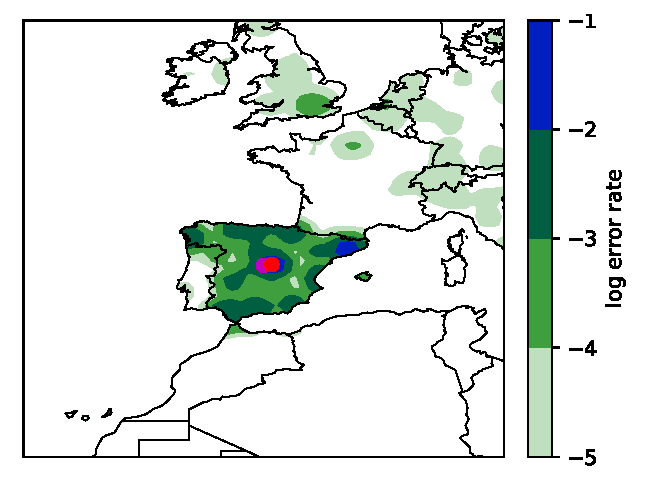
\includegraphics{img/infer/es-vosotros-good/1-med-zoom}} &
        %\resizebox{0.3\textwidth}{!}{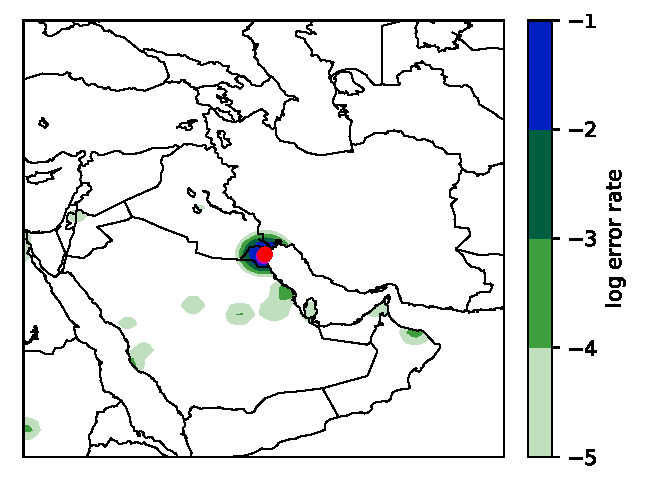
\includegraphics{img/infer/ar-kuwait-japanese/0-med-zoom}} &
        %\resizebox{0.3\textwidth}{!}{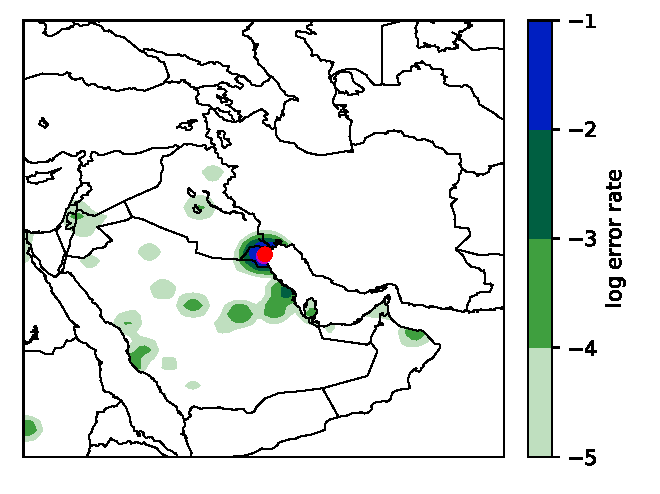
\includegraphics{img/infer/ar-kuwait-japanese/5-med-zoom}} &
        %\\
        %\small
        %\str{Qu\'e gran ma\~nana... emocionante.  Pod\'eis ver el v\'ideo abajo en el enlace.}%
        %&
        %\str{I'm at }\foreignlanguage{arabic}{شارع المطاعم}\str{ in }
       % 
        %\foreignlanguage{arabic}{الكويت}.%
        %&
        %\str{I'm at }\begin{CJK}{UTF8}{min}通りレストラン\end{CJK}\str{ in }
        %\begin{CJK}{UTF8}{min}クウェート\end{CJK}.
    %\end{tabular}
    %\caption{test}
    %\label{fig:poder}
%\end{figure*}

%%%%%%%%%%%%%%%%%%%%%%%%%%%%%%%%%%%%%%%%%%%%%%%%%%%%%%%%%%%%%%%%%%%%%%%%%%%%%%%%

\section{Introduction}

Social media platforms are becoming increasingly multilingual.
More than 100 languages are known to be actively used on Twitter \citep{hong2011language},
and while English is still the most popular, its popularity is shrinking.
An analysis of tweets sent in 2012 found that 53\% of tweets were written in English \citep{han2014text},
but our analysis of tweets sent in 2018 shows that only 42\% of tweets were written in English.
%While English and other popular languages have been well studied,
%less popular languages have received relatively little attention.
%This is unfortunate because approximately 80 million tweets are sent everyday in a language that is not one of Twitter's ten most popular languages.
This percentage will likely continue to fall
as more people in non-English speaking countries connect to the internet and begin using social media.
%Approximately 16\% of tweets are sent in either a language that Twitter doesn't officially support or one of Twitter's 55 least popular official languages.
%In absolute numbers, this is about 80 million tweets per day.
%Approximately 8\% of tweets are sent in Twitter's 55 least popular languages,
%and a further 8\% of tweets are sent in languages that the Twitter API does not officially support.
New multilingual data analysis tools are needed to better serve these emerging non-English communities.
%Many language communities are poorly served by state-of-the-art text analysis tools,
%which are designed for English and similarly popular languages.
%Better data analysis tools are need to serve these non-English communities.
%Good methods for analyzing multilingual social text is therefore highly important
%and understudied.

This paper introduces the \defn{Unicode Convolutional Neural Network} (UnicodeCNN) for analyzing multilingual social media text.
The UnicodeCNN generates features directly from the Unicode characters in the input text and requires no lexical analysis, stemming, or other preprocessing.
Character-level convolutional neural networks have previously been successfully applied to text corpora containing only English \citep{zhang2015character,conneau2017very} or a limited number of European languages \citep{lee2016fully,wehrmann2017character},
but our UnicodeCNN can take any Unicode string as input and therefore works with all languages.
We use the same model to analyze English, Arabic, Japanese, and the more than 100 languages present in our Twitter dataset.
%Amazingly, we show that information learned in one language can be transfered to other languages.
%Many bi-lingual models have been developed for various natural language tasks,
%but multi-lingual models remain rare \citep{ruder2017survey}.
%We believe the UnicodeCNN is the first model designed to work on all languages simultaneously.
The UnicodeCNN is particularly well-suited to analyzing social media text because it is naturally robust to the spelling mistakes and non-standard grammar commonly found in this domain.
%As an extreme example, \defn{Arabizi} is a newly developing dialect of the Arabic language found only in social media platforms.
%Arabizi consists of a mixture of Latin and Arabic characters in a single message,

We apply the UnicodeCNN to the challenging problem of \defn{content-based tweet geolocation},
or predicting the GPS coordinates a tweet was sent from based only on its text.
Geolocation is a well-studied problem,
and our UnicodeCNN significantly improves the state-of-the-art in three ways.
First, most prior work considers only English-language tweets \citep{cheng2010you,kinsella2011m,li2012towards,han2013stacking,mahmud2014home,compton2014geotagging,zhang2014geocoding,rahimi2015twitter,dredze2016geolocation,rahimi2017neural},
or tweets in a single non-English language like Spanish \citep{maier2014language,gonccalves2015learning,tinoco2017variation}. % or Italian \citep{paraskevopoulos2015fine}.
\citet{han2014text} propose a multilingual system that first detects the language of the tweet,
then passes the tweet to an appropriate single-language model.
Each of these single-language models must be developed independently and from scratch,
and \citet{han2014text} only support Twitter's most popular languages.
The UnicodeCNN, in contrast, processes all languages in a unified method.
Remarkably, we show that geographic information learned in one language is automatically learned in other languages as well.
Second, all previous work considered only a subset of tweets that were particularly easy to geolocate.
In particular, all works cited above filter their datasets to contain only tweets sent from certain countries or major cities.
We perform no such filtering because our method works on all tweets, written in all languages, sent from anywhere in the world.
%The UnicodeCNN generates high quality features that work everywhere in the world,
%and so we perform no such filtering in our experiments.
Finally, most previous work solves a classification problem,
where each tweet is associated with either its country or city of origin.
%Two papers \citep{thomas2017twitter,duong2016near} propose to learn the exact GPS coordinates of tweets,
%but fail to consider the non-Euclidean nature of the Earth's surface.
We instead use a mixture of Fischer-von Mises distributions to predict the exact GPS location of tweets.
We show that the high quality features generated by the UnicodeCNN enable us to solve this more challenging prediction problem.
%We introduce a new technique based on the mixture of Fisher-von Mises distributions that lets us accurately predict the exact GPS location of tweets. 

%We evaluate the UnicodeCNN on the twitter geolocation task for two reasons.
%First, geolocation has many important applications.
Tweet geolocation has many important applications.
Geotagged tweets have been used to map the spread of influenza \citep{paul2014twitter,santillana2015combining},
for measuring the impact of earthquakes \citep{sakaki2010earthquake},
for coordinating emergency services \citep{klein2012detection,rudra2016summarizing},%imran2016twitter,pohl2016online,
for measuring the spread of political opinions \citep{conover2011political,barbera2014birds},
for comparing dietary habits in different locations \citep{widener2014using},
for measuring neighborhood happiness levels \citep{nguyen2016leveraging}, 
and for measuring unemployment rates \citep{antenucci2014using,llorente2015social}.
Unfortunately for these applications, only about 1\% of tweets are geotagged by their users.
Our system can predict the location of the other 99\% of tweets and therefore improve the accuracy and applicability of all of these methods.

\ignore{
Second, we believe our UnicodeCNN trained on 
Finally, geolocated tweets provide a large source of high quality labeled text.
Quality labeled text is rare and often the limitting factor in natural language processing tasks.
Transfer learning has therefore become a popular strategy to learn these tasks \citep{wang2015transfer,howard2018fine}.
The model we develop is particularly suitable for transfer learning because it incorporates many languages.
We open source our model and a toolkit to help practitioners use this model as the base for other multilingual NLP tasks.
}

\ignore{
\begin{description}
%\begin{description}
\item[Why care about geolocation?]
    Geolocating tweets is an important problem for three reasons.

First, many important applications require geolocated tweets as input.
For example, geotagged tweets have been used to map the spread of influenza \citep{paul2014twitter,santillana2015combining},
for measuring the impact of earthquakes \citep{sakaki2010earthquake},
for coordinating emergency services \citep{klein2012detection,imran2016twitter,rudra2016summarizing,pohl2016online},
for measuring the spread of political opinions \citep{conover2011political,barbera2014birds},
for comparing dietary habits in different locations \citep{widener2014using},
for measuring neighborhood happiness levels \citep{nguyen2016leveraging}, 
and for measuring unemployment rates \citep{antenucci2014using,llorente2015social}.
Unfortunately for these applications, only about 1\% of tweets are geotagged by their users.
A system that could predict the location of the other 99\% of tweets would immediately improve the accuracy and applicability of all of these methods.

Second, the models used for geotagging tweets help us understand the differences between different languages and dialects.
For example, previous work has used geotagged language models to map the dialects of Standard American English versus African-American English \citep{huang2016understanding,gonccalves2017fall,blodgett2016demographic}. %, and the various dialects of Spanish \citep{gonccalves2014crowdsourcing}.
%Our language model is more advanced than previous models because it works for significantly more languages,
%and it operates on the character level rather than the word level.
%This more advanced model lets learn more detail about dialectical differences in many more languages than previous work.
Our language model is the first to operate on the character level using a highly multilingual dataset.
Therefore, we can map significantly more dialectical variations in language useage than previous work.

Finally, geolocated tweets provide a large source of high quality labeled text.
Quality labeled text is rare and often the limitting factor in natural language processing tasks.
Transfer learning has therefore become a popular strategy to learn these tasks \citep{wang2015transfer,howard2018fine}.
The model we develop is particularly suitable for transfer learning because it incorporates many languages.
We open source our model and a toolkit to help practitioners use this model as the base for other multilingual NLP tasks.
%Furthermore, because our language model combines so many different languages,
%and can form the basis for multilingual classification tasks using transfer learning \citep{wang2015transfer,howard2018fine}.
%The best existing image transfer learning used billions of Instagram images labelled by their hashtags from FAIR \citep{mahajan2018exploring}.
}

\ignore{
\item[Our contributions.]
Our contributions include:
\begin{enumerate}
    \item
        Our method works with all tweets, in all languages.
        Twitter has official support for XXX languages,
        but many other languages are represented as well.
        For example, nearly-dead languages like Latin.
        The pope has an official latin-only twitter account \str{@Pontifex\_ln}.
        The esperanto language is not officially supported, but has an active twitter community.
        And web aps will automatically translate a text into Klingon\footnote{The ap appears to have been taken offline, but a news article is available at https://www.tomsguide.com/us/Star-Trek-Online-Klingon-Translator,news-5294.html} and tweet it.
    \item
        Our method requires no ad-hoc preprocessing of the data,
        and in particular can achieve good results with only a single pass over the dataset.
    \item
        A new method for generating features at the character level.
    \item
        Our method can output gps coordinates and take advantage of the non-Euclidean geometry of the Earth's surface.
    \item
        A general framework that lets us easily mix and match the contributions from previous works.
    \item
        An online learning framework that is more natural for twitter than the batch frameworks previously proposed.
    \item
        \fixme{todo}
        A method for visualizing the important features that causes a tweet to be located in a particular location.
\end{enumerate}
}

\begin{description}
\item[Paper Outline.]
\fixme{
The next section demonstrates the qualitative advantages of the UnicodeCNN.
Then in Section \ref{sec:words} we describe in detail why the word-level approach of previous geolocation systems cannot scale to the massively multilingual dataset we use.
In Section \ref{sec:model} we introduce our character level model that fixes the deficiencies of the world-level models.
We also describe two novel neural network output layers called angualar regression and the mixture of von-Mises,
and show how these methods take advantage of the geometry of the Earth's surface to enable us to predict exact GPS coordinates of a tweet.
Section \ref{sec:experiments} shows the experimental results showing that our method significantly outperforms previous methods.
}

\end{description}

%%%%%%%%%%%%%%%%%%%%%%%%%%%%%%%%%%%%%%%%
%\subsection{Identifying tweet location vs user location}
%
%In this paper, we focus on the task of identifying tweet location, rather than user location.
%Identifying the location of a tweet is the harder problem because there is less information available.

%%%%%%%%%%%%%%%%%%%%%%%%%%%%%%%%%%%%%%%%%%%%%%%%%%%%%%%%%%%%%%%%%%%%%%%%%%%%%%%%
\section{Qualitative Overview}

Before describing our model in detail,
we present some simple examples.
We use these examples to introduce the details of the geolocation problem,
and demonstrate the qualitative ability of the UnicodeCNN to learn complex language features.

%We now consider two examples that illustrate the difficulty of the geolocation problem and the power of the UnicodeCNN compared with other methods.

%%%%%%%%%%%%%%%%%%%%%%%%%%%%%%%%%%%%%%%%

  %\captionsetup{labelfont={bf},
  %textfont={bf}, labelsep=colon}
\begin{figure}
    \resizebox{0.485\textwidth}{!}{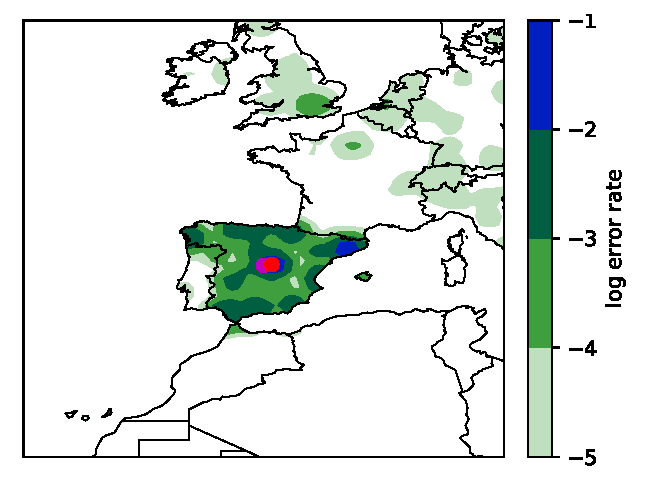
\includegraphics{img/infer/es-vosotros-good/1-med-zoom}}
    \vspace{-1cm}

    \textbf{
    \caption{
    %The probability distribution of where our model locates the tweet in Example 1 below.
        For each tweet, our model outputs a distribution over the Earth's surface that represents the likelihood that the tweet was sent from that location.
        This map shows the distribution for the tweet \str{No me hablen} in Example 1 below.
    \fixme{Beautify.}
    \label{fig:poder}
    }
}
\end{figure}

%%%%%%%%%%%%%%%%%%%%%%%%%%%%%%%%%%%%%%%%

\begin{description}
\item[Example 1.]
%We begin with an example that illustrates the difficulty of the problem.
%We now consider an example which illustrates the difficulty of the geolocation problem and the power of the UnicodeCNN model.
%Let's try to guess where the following tweet was sent from:
    %Consider the following real tweet:
    %Let's try to guess where the following tweet was sent from:
    %This example illustrates the difficulty of the geolocaiton problem by showing how location information is encoded in subtle linguistic patterns within a tweet.
    Our first example illustrates how the UnicodeCNN is able to learn verb conjugation rules and use them for geolocation.
    %Different dialects of the same language use different verb conjugation rules,
    %and we use this fact to geolocate tweets.
    %Remarkably, our model is able to understand conjugations of verbs it has never been trained on and is robust to misspellings.
    Consider the following short Spanish tweet:%
%\begin{quote}
    %\str{Qu\'e gran ma\~nana... emocionante.  Pod\'eis ver el v\'ideo abajo en el enlace.}%
    %\footnote{Translation: ``What a great morning... exciting.  You can see the video below the post.''}
%\end{quote}
    %\footnote{Tweet ID: 927275629061591040.}
    \begin{quote}
        \str{No me habl\'eis}
    \end{quote}
    which translates as
    \begin{quote}
        \str{Don't speak to me}
    \end{quote}
Figure \ref{fig:poder} shows the GPS coordinates that our model predicts this tweet was sent from,
%and here's the top three predicted countries:
and the plot below shows the model's top three predicted countries and associated probabilities.

\noindent%% Creator: Matplotlib, PGF backend
%%
%% To include the figure in your LaTeX document, write
%%   \input{<filename>.pgf}
%%
%% Make sure the required packages are loaded in your preamble
%%   \usepackage{pgf}
%%
%% Figures using additional raster images can only be included by \input if
%% they are in the same directory as the main LaTeX file. For loading figures
%% from other directories you can use the `import` package
%%   \usepackage{import}
%% and then include the figures with
%%   \import{<path to file>}{<filename>.pgf}
%%
%% Matplotlib used the following preamble
%%   \usepackage{fontspec}
%%
\begingroup%
\makeatletter%
\begin{pgfpicture}%
\pgfpathrectangle{\pgfpointorigin}{\pgfqpoint{3.500000in}{0.700000in}}%
\pgfusepath{use as bounding box, clip}%
\begin{pgfscope}%
\pgfsetbuttcap%
\pgfsetmiterjoin%
\definecolor{currentfill}{rgb}{1.000000,1.000000,1.000000}%
\pgfsetfillcolor{currentfill}%
\pgfsetlinewidth{0.000000pt}%
\definecolor{currentstroke}{rgb}{1.000000,1.000000,1.000000}%
\pgfsetstrokecolor{currentstroke}%
\pgfsetdash{}{0pt}%
\pgfpathmoveto{\pgfqpoint{0.000000in}{0.000000in}}%
\pgfpathlineto{\pgfqpoint{3.500000in}{0.000000in}}%
\pgfpathlineto{\pgfqpoint{3.500000in}{0.700000in}}%
\pgfpathlineto{\pgfqpoint{0.000000in}{0.700000in}}%
\pgfpathclose%
\pgfusepath{fill}%
\end{pgfscope}%
\begin{pgfscope}%
\pgfsetbuttcap%
\pgfsetmiterjoin%
\definecolor{currentfill}{rgb}{1.000000,1.000000,1.000000}%
\pgfsetfillcolor{currentfill}%
\pgfsetlinewidth{0.000000pt}%
\definecolor{currentstroke}{rgb}{0.000000,0.000000,0.000000}%
\pgfsetstrokecolor{currentstroke}%
\pgfsetstrokeopacity{0.000000}%
\pgfsetdash{}{0pt}%
\pgfpathmoveto{\pgfqpoint{1.050000in}{0.245000in}}%
\pgfpathlineto{\pgfqpoint{3.150000in}{0.245000in}}%
\pgfpathlineto{\pgfqpoint{3.150000in}{0.616000in}}%
\pgfpathlineto{\pgfqpoint{1.050000in}{0.616000in}}%
\pgfpathclose%
\pgfusepath{fill}%
\end{pgfscope}%
\begin{pgfscope}%
\pgfpathrectangle{\pgfqpoint{1.050000in}{0.245000in}}{\pgfqpoint{2.100000in}{0.371000in}} %
\pgfusepath{clip}%
\pgfsetbuttcap%
\pgfsetmiterjoin%
\definecolor{currentfill}{rgb}{0.000000,0.501961,0.000000}%
\pgfsetfillcolor{currentfill}%
\pgfsetlinewidth{0.000000pt}%
\definecolor{currentstroke}{rgb}{0.000000,0.000000,0.000000}%
\pgfsetstrokecolor{currentstroke}%
\pgfsetstrokeopacity{0.000000}%
\pgfsetdash{}{0pt}%
\pgfpathmoveto{\pgfqpoint{1.050000in}{0.599136in}}%
\pgfpathlineto{\pgfqpoint{2.428962in}{0.599136in}}%
\pgfpathlineto{\pgfqpoint{2.428962in}{0.502773in}}%
\pgfpathlineto{\pgfqpoint{1.050000in}{0.502773in}}%
\pgfpathclose%
\pgfusepath{fill}%
\end{pgfscope}%
\begin{pgfscope}%
\pgfpathrectangle{\pgfqpoint{1.050000in}{0.245000in}}{\pgfqpoint{2.100000in}{0.371000in}} %
\pgfusepath{clip}%
\pgfsetbuttcap%
\pgfsetmiterjoin%
\definecolor{currentfill}{rgb}{0.000000,0.501961,0.000000}%
\pgfsetfillcolor{currentfill}%
\pgfsetlinewidth{0.000000pt}%
\definecolor{currentstroke}{rgb}{0.000000,0.000000,0.000000}%
\pgfsetstrokecolor{currentstroke}%
\pgfsetstrokeopacity{0.000000}%
\pgfsetdash{}{0pt}%
\pgfpathmoveto{\pgfqpoint{1.050000in}{0.478682in}}%
\pgfpathlineto{\pgfqpoint{1.217107in}{0.478682in}}%
\pgfpathlineto{\pgfqpoint{1.217107in}{0.382318in}}%
\pgfpathlineto{\pgfqpoint{1.050000in}{0.382318in}}%
\pgfpathclose%
\pgfusepath{fill}%
\end{pgfscope}%
\begin{pgfscope}%
\pgfpathrectangle{\pgfqpoint{1.050000in}{0.245000in}}{\pgfqpoint{2.100000in}{0.371000in}} %
\pgfusepath{clip}%
\pgfsetbuttcap%
\pgfsetmiterjoin%
\definecolor{currentfill}{rgb}{0.000000,0.501961,0.000000}%
\pgfsetfillcolor{currentfill}%
\pgfsetlinewidth{0.000000pt}%
\definecolor{currentstroke}{rgb}{0.000000,0.000000,0.000000}%
\pgfsetstrokecolor{currentstroke}%
\pgfsetstrokeopacity{0.000000}%
\pgfsetdash{}{0pt}%
\pgfpathmoveto{\pgfqpoint{1.050000in}{0.358227in}}%
\pgfpathlineto{\pgfqpoint{1.197415in}{0.358227in}}%
\pgfpathlineto{\pgfqpoint{1.197415in}{0.261864in}}%
\pgfpathlineto{\pgfqpoint{1.050000in}{0.261864in}}%
\pgfpathclose%
\pgfusepath{fill}%
\end{pgfscope}%
\begin{pgfscope}%
\pgfsetbuttcap%
\pgfsetroundjoin%
\definecolor{currentfill}{rgb}{0.000000,0.000000,0.000000}%
\pgfsetfillcolor{currentfill}%
\pgfsetlinewidth{0.803000pt}%
\definecolor{currentstroke}{rgb}{0.000000,0.000000,0.000000}%
\pgfsetstrokecolor{currentstroke}%
\pgfsetdash{}{0pt}%
\pgfsys@defobject{currentmarker}{\pgfqpoint{0.000000in}{-0.048611in}}{\pgfqpoint{0.000000in}{0.000000in}}{%
\pgfpathmoveto{\pgfqpoint{0.000000in}{0.000000in}}%
\pgfpathlineto{\pgfqpoint{0.000000in}{-0.048611in}}%
\pgfusepath{stroke,fill}%
}%
\begin{pgfscope}%
\pgfsys@transformshift{1.050000in}{0.245000in}%
\pgfsys@useobject{currentmarker}{}%
\end{pgfscope}%
\end{pgfscope}%
\begin{pgfscope}%
\pgftext[x=1.050000in,y=0.147778in,,top]{\sffamily\fontsize{8.000000}{9.600000}\selectfont 0.0}%
\end{pgfscope}%
\begin{pgfscope}%
\pgfsetbuttcap%
\pgfsetroundjoin%
\definecolor{currentfill}{rgb}{0.000000,0.000000,0.000000}%
\pgfsetfillcolor{currentfill}%
\pgfsetlinewidth{0.803000pt}%
\definecolor{currentstroke}{rgb}{0.000000,0.000000,0.000000}%
\pgfsetstrokecolor{currentstroke}%
\pgfsetdash{}{0pt}%
\pgfsys@defobject{currentmarker}{\pgfqpoint{0.000000in}{-0.048611in}}{\pgfqpoint{0.000000in}{0.000000in}}{%
\pgfpathmoveto{\pgfqpoint{0.000000in}{0.000000in}}%
\pgfpathlineto{\pgfqpoint{0.000000in}{-0.048611in}}%
\pgfusepath{stroke,fill}%
}%
\begin{pgfscope}%
\pgfsys@transformshift{1.470000in}{0.245000in}%
\pgfsys@useobject{currentmarker}{}%
\end{pgfscope}%
\end{pgfscope}%
\begin{pgfscope}%
\pgftext[x=1.470000in,y=0.147778in,,top]{\sffamily\fontsize{8.000000}{9.600000}\selectfont 0.2}%
\end{pgfscope}%
\begin{pgfscope}%
\pgfsetbuttcap%
\pgfsetroundjoin%
\definecolor{currentfill}{rgb}{0.000000,0.000000,0.000000}%
\pgfsetfillcolor{currentfill}%
\pgfsetlinewidth{0.803000pt}%
\definecolor{currentstroke}{rgb}{0.000000,0.000000,0.000000}%
\pgfsetstrokecolor{currentstroke}%
\pgfsetdash{}{0pt}%
\pgfsys@defobject{currentmarker}{\pgfqpoint{0.000000in}{-0.048611in}}{\pgfqpoint{0.000000in}{0.000000in}}{%
\pgfpathmoveto{\pgfqpoint{0.000000in}{0.000000in}}%
\pgfpathlineto{\pgfqpoint{0.000000in}{-0.048611in}}%
\pgfusepath{stroke,fill}%
}%
\begin{pgfscope}%
\pgfsys@transformshift{1.890000in}{0.245000in}%
\pgfsys@useobject{currentmarker}{}%
\end{pgfscope}%
\end{pgfscope}%
\begin{pgfscope}%
\pgftext[x=1.890000in,y=0.147778in,,top]{\sffamily\fontsize{8.000000}{9.600000}\selectfont 0.4}%
\end{pgfscope}%
\begin{pgfscope}%
\pgfsetbuttcap%
\pgfsetroundjoin%
\definecolor{currentfill}{rgb}{0.000000,0.000000,0.000000}%
\pgfsetfillcolor{currentfill}%
\pgfsetlinewidth{0.803000pt}%
\definecolor{currentstroke}{rgb}{0.000000,0.000000,0.000000}%
\pgfsetstrokecolor{currentstroke}%
\pgfsetdash{}{0pt}%
\pgfsys@defobject{currentmarker}{\pgfqpoint{0.000000in}{-0.048611in}}{\pgfqpoint{0.000000in}{0.000000in}}{%
\pgfpathmoveto{\pgfqpoint{0.000000in}{0.000000in}}%
\pgfpathlineto{\pgfqpoint{0.000000in}{-0.048611in}}%
\pgfusepath{stroke,fill}%
}%
\begin{pgfscope}%
\pgfsys@transformshift{2.310000in}{0.245000in}%
\pgfsys@useobject{currentmarker}{}%
\end{pgfscope}%
\end{pgfscope}%
\begin{pgfscope}%
\pgftext[x=2.310000in,y=0.147778in,,top]{\sffamily\fontsize{8.000000}{9.600000}\selectfont 0.6}%
\end{pgfscope}%
\begin{pgfscope}%
\pgfsetbuttcap%
\pgfsetroundjoin%
\definecolor{currentfill}{rgb}{0.000000,0.000000,0.000000}%
\pgfsetfillcolor{currentfill}%
\pgfsetlinewidth{0.803000pt}%
\definecolor{currentstroke}{rgb}{0.000000,0.000000,0.000000}%
\pgfsetstrokecolor{currentstroke}%
\pgfsetdash{}{0pt}%
\pgfsys@defobject{currentmarker}{\pgfqpoint{0.000000in}{-0.048611in}}{\pgfqpoint{0.000000in}{0.000000in}}{%
\pgfpathmoveto{\pgfqpoint{0.000000in}{0.000000in}}%
\pgfpathlineto{\pgfqpoint{0.000000in}{-0.048611in}}%
\pgfusepath{stroke,fill}%
}%
\begin{pgfscope}%
\pgfsys@transformshift{2.730000in}{0.245000in}%
\pgfsys@useobject{currentmarker}{}%
\end{pgfscope}%
\end{pgfscope}%
\begin{pgfscope}%
\pgftext[x=2.730000in,y=0.147778in,,top]{\sffamily\fontsize{8.000000}{9.600000}\selectfont 0.8}%
\end{pgfscope}%
\begin{pgfscope}%
\pgfsetbuttcap%
\pgfsetroundjoin%
\definecolor{currentfill}{rgb}{0.000000,0.000000,0.000000}%
\pgfsetfillcolor{currentfill}%
\pgfsetlinewidth{0.803000pt}%
\definecolor{currentstroke}{rgb}{0.000000,0.000000,0.000000}%
\pgfsetstrokecolor{currentstroke}%
\pgfsetdash{}{0pt}%
\pgfsys@defobject{currentmarker}{\pgfqpoint{0.000000in}{-0.048611in}}{\pgfqpoint{0.000000in}{0.000000in}}{%
\pgfpathmoveto{\pgfqpoint{0.000000in}{0.000000in}}%
\pgfpathlineto{\pgfqpoint{0.000000in}{-0.048611in}}%
\pgfusepath{stroke,fill}%
}%
\begin{pgfscope}%
\pgfsys@transformshift{3.150000in}{0.245000in}%
\pgfsys@useobject{currentmarker}{}%
\end{pgfscope}%
\end{pgfscope}%
\begin{pgfscope}%
\pgftext[x=3.150000in,y=0.147778in,,top]{\sffamily\fontsize{8.000000}{9.600000}\selectfont 1.0}%
\end{pgfscope}%
\begin{pgfscope}%
\pgfsetbuttcap%
\pgfsetroundjoin%
\definecolor{currentfill}{rgb}{0.000000,0.000000,0.000000}%
\pgfsetfillcolor{currentfill}%
\pgfsetlinewidth{0.803000pt}%
\definecolor{currentstroke}{rgb}{0.000000,0.000000,0.000000}%
\pgfsetstrokecolor{currentstroke}%
\pgfsetdash{}{0pt}%
\pgfsys@defobject{currentmarker}{\pgfqpoint{-0.048611in}{0.000000in}}{\pgfqpoint{0.000000in}{0.000000in}}{%
\pgfpathmoveto{\pgfqpoint{0.000000in}{0.000000in}}%
\pgfpathlineto{\pgfqpoint{-0.048611in}{0.000000in}}%
\pgfusepath{stroke,fill}%
}%
\begin{pgfscope}%
\pgfsys@transformshift{1.050000in}{0.550955in}%
\pgfsys@useobject{currentmarker}{}%
\end{pgfscope}%
\end{pgfscope}%
\begin{pgfscope}%
\pgftext[x=0.680444in,y=0.511232in,left,base]{\sffamily\fontsize{8.000000}{9.600000}\selectfont Spain}%
\end{pgfscope}%
\begin{pgfscope}%
\pgfsetbuttcap%
\pgfsetroundjoin%
\definecolor{currentfill}{rgb}{0.000000,0.000000,0.000000}%
\pgfsetfillcolor{currentfill}%
\pgfsetlinewidth{0.803000pt}%
\definecolor{currentstroke}{rgb}{0.000000,0.000000,0.000000}%
\pgfsetstrokecolor{currentstroke}%
\pgfsetdash{}{0pt}%
\pgfsys@defobject{currentmarker}{\pgfqpoint{-0.048611in}{0.000000in}}{\pgfqpoint{0.000000in}{0.000000in}}{%
\pgfpathmoveto{\pgfqpoint{0.000000in}{0.000000in}}%
\pgfpathlineto{\pgfqpoint{-0.048611in}{0.000000in}}%
\pgfusepath{stroke,fill}%
}%
\begin{pgfscope}%
\pgfsys@transformshift{1.050000in}{0.430500in}%
\pgfsys@useobject{currentmarker}{}%
\end{pgfscope}%
\end{pgfscope}%
\begin{pgfscope}%
\pgftext[x=0.472889in,y=0.391944in,left,base]{\sffamily\fontsize{8.000000}{9.600000}\selectfont Argentina}%
\end{pgfscope}%
\begin{pgfscope}%
\pgfsetbuttcap%
\pgfsetroundjoin%
\definecolor{currentfill}{rgb}{0.000000,0.000000,0.000000}%
\pgfsetfillcolor{currentfill}%
\pgfsetlinewidth{0.803000pt}%
\definecolor{currentstroke}{rgb}{0.000000,0.000000,0.000000}%
\pgfsetstrokecolor{currentstroke}%
\pgfsetdash{}{0pt}%
\pgfsys@defobject{currentmarker}{\pgfqpoint{-0.048611in}{0.000000in}}{\pgfqpoint{0.000000in}{0.000000in}}{%
\pgfpathmoveto{\pgfqpoint{0.000000in}{0.000000in}}%
\pgfpathlineto{\pgfqpoint{-0.048611in}{0.000000in}}%
\pgfusepath{stroke,fill}%
}%
\begin{pgfscope}%
\pgfsys@transformshift{1.050000in}{0.310045in}%
\pgfsys@useobject{currentmarker}{}%
\end{pgfscope}%
\end{pgfscope}%
\begin{pgfscope}%
\pgftext[x=0.282000in,y=0.271490in,left,base]{\sffamily\fontsize{8.000000}{9.600000}\selectfont United States}%
\end{pgfscope}%
\begin{pgfscope}%
\pgfsetrectcap%
\pgfsetmiterjoin%
\pgfsetlinewidth{0.803000pt}%
\definecolor{currentstroke}{rgb}{0.000000,0.000000,0.000000}%
\pgfsetstrokecolor{currentstroke}%
\pgfsetdash{}{0pt}%
\pgfpathmoveto{\pgfqpoint{1.050000in}{0.245000in}}%
\pgfpathlineto{\pgfqpoint{1.050000in}{0.616000in}}%
\pgfusepath{stroke}%
\end{pgfscope}%
\begin{pgfscope}%
\pgfsetrectcap%
\pgfsetmiterjoin%
\pgfsetlinewidth{0.803000pt}%
\definecolor{currentstroke}{rgb}{0.000000,0.000000,0.000000}%
\pgfsetstrokecolor{currentstroke}%
\pgfsetdash{}{0pt}%
\pgfpathmoveto{\pgfqpoint{1.050000in}{0.245000in}}%
\pgfpathlineto{\pgfqpoint{3.150000in}{0.245000in}}%
\pgfusepath{stroke}%
\end{pgfscope}%
\end{pgfpicture}%
\makeatother%
\endgroup%


\noindent
This tweet was in fact sent from Spain as our model predicts.
Our model made this prediction by learning that the word \str{habl\'eis} is a conjugation of the verb \str{hablar} in the vosotros form,
which is only used in the Castilian Spanish dialect of Spain.
American Spanish dialects instead use the ustedes form instead,
which conjugates the verb as \str{hablen}.
If we modify the tweet to use the American Spanish dialect:
\begin{quote}
    \str{No me hablen}
\end{quote}
%
%word \str{hablen} instead of \str{habl\'eis},
then the model's predictions change accordingly:

\noindent%% Creator: Matplotlib, PGF backend
%%
%% To include the figure in your LaTeX document, write
%%   \input{<filename>.pgf}
%%
%% Make sure the required packages are loaded in your preamble
%%   \usepackage{pgf}
%%
%% Figures using additional raster images can only be included by \input if
%% they are in the same directory as the main LaTeX file. For loading figures
%% from other directories you can use the `import` package
%%   \usepackage{import}
%% and then include the figures with
%%   \import{<path to file>}{<filename>.pgf}
%%
%% Matplotlib used the following preamble
%%   \usepackage{fontspec}
%%
\begingroup%
\makeatletter%
\begin{pgfpicture}%
\pgfpathrectangle{\pgfpointorigin}{\pgfqpoint{3.500000in}{0.700000in}}%
\pgfusepath{use as bounding box, clip}%
\begin{pgfscope}%
\pgfsetbuttcap%
\pgfsetmiterjoin%
\definecolor{currentfill}{rgb}{1.000000,1.000000,1.000000}%
\pgfsetfillcolor{currentfill}%
\pgfsetlinewidth{0.000000pt}%
\definecolor{currentstroke}{rgb}{1.000000,1.000000,1.000000}%
\pgfsetstrokecolor{currentstroke}%
\pgfsetdash{}{0pt}%
\pgfpathmoveto{\pgfqpoint{0.000000in}{0.000000in}}%
\pgfpathlineto{\pgfqpoint{3.500000in}{0.000000in}}%
\pgfpathlineto{\pgfqpoint{3.500000in}{0.700000in}}%
\pgfpathlineto{\pgfqpoint{0.000000in}{0.700000in}}%
\pgfpathclose%
\pgfusepath{fill}%
\end{pgfscope}%
\begin{pgfscope}%
\pgfsetbuttcap%
\pgfsetmiterjoin%
\definecolor{currentfill}{rgb}{1.000000,1.000000,1.000000}%
\pgfsetfillcolor{currentfill}%
\pgfsetlinewidth{0.000000pt}%
\definecolor{currentstroke}{rgb}{0.000000,0.000000,0.000000}%
\pgfsetstrokecolor{currentstroke}%
\pgfsetstrokeopacity{0.000000}%
\pgfsetdash{}{0pt}%
\pgfpathmoveto{\pgfqpoint{1.050000in}{0.245000in}}%
\pgfpathlineto{\pgfqpoint{3.150000in}{0.245000in}}%
\pgfpathlineto{\pgfqpoint{3.150000in}{0.616000in}}%
\pgfpathlineto{\pgfqpoint{1.050000in}{0.616000in}}%
\pgfpathclose%
\pgfusepath{fill}%
\end{pgfscope}%
\begin{pgfscope}%
\pgfpathrectangle{\pgfqpoint{1.050000in}{0.245000in}}{\pgfqpoint{2.100000in}{0.371000in}} %
\pgfusepath{clip}%
\pgfsetbuttcap%
\pgfsetmiterjoin%
\definecolor{currentfill}{rgb}{0.000000,0.501961,0.000000}%
\pgfsetfillcolor{currentfill}%
\pgfsetlinewidth{0.000000pt}%
\definecolor{currentstroke}{rgb}{0.000000,0.000000,0.000000}%
\pgfsetstrokecolor{currentstroke}%
\pgfsetstrokeopacity{0.000000}%
\pgfsetdash{}{0pt}%
\pgfpathmoveto{\pgfqpoint{1.050000in}{0.599136in}}%
\pgfpathlineto{\pgfqpoint{1.684730in}{0.599136in}}%
\pgfpathlineto{\pgfqpoint{1.684730in}{0.502773in}}%
\pgfpathlineto{\pgfqpoint{1.050000in}{0.502773in}}%
\pgfpathclose%
\pgfusepath{fill}%
\end{pgfscope}%
\begin{pgfscope}%
\pgfpathrectangle{\pgfqpoint{1.050000in}{0.245000in}}{\pgfqpoint{2.100000in}{0.371000in}} %
\pgfusepath{clip}%
\pgfsetbuttcap%
\pgfsetmiterjoin%
\definecolor{currentfill}{rgb}{0.000000,0.501961,0.000000}%
\pgfsetfillcolor{currentfill}%
\pgfsetlinewidth{0.000000pt}%
\definecolor{currentstroke}{rgb}{0.000000,0.000000,0.000000}%
\pgfsetstrokecolor{currentstroke}%
\pgfsetstrokeopacity{0.000000}%
\pgfsetdash{}{0pt}%
\pgfpathmoveto{\pgfqpoint{1.050000in}{0.478682in}}%
\pgfpathlineto{\pgfqpoint{1.606497in}{0.478682in}}%
\pgfpathlineto{\pgfqpoint{1.606497in}{0.382318in}}%
\pgfpathlineto{\pgfqpoint{1.050000in}{0.382318in}}%
\pgfpathclose%
\pgfusepath{fill}%
\end{pgfscope}%
\begin{pgfscope}%
\pgfpathrectangle{\pgfqpoint{1.050000in}{0.245000in}}{\pgfqpoint{2.100000in}{0.371000in}} %
\pgfusepath{clip}%
\pgfsetbuttcap%
\pgfsetmiterjoin%
\definecolor{currentfill}{rgb}{0.000000,0.501961,0.000000}%
\pgfsetfillcolor{currentfill}%
\pgfsetlinewidth{0.000000pt}%
\definecolor{currentstroke}{rgb}{0.000000,0.000000,0.000000}%
\pgfsetstrokecolor{currentstroke}%
\pgfsetstrokeopacity{0.000000}%
\pgfsetdash{}{0pt}%
\pgfpathmoveto{\pgfqpoint{1.050000in}{0.358227in}}%
\pgfpathlineto{\pgfqpoint{1.274502in}{0.358227in}}%
\pgfpathlineto{\pgfqpoint{1.274502in}{0.261864in}}%
\pgfpathlineto{\pgfqpoint{1.050000in}{0.261864in}}%
\pgfpathclose%
\pgfusepath{fill}%
\end{pgfscope}%
\begin{pgfscope}%
\pgfsetbuttcap%
\pgfsetroundjoin%
\definecolor{currentfill}{rgb}{0.000000,0.000000,0.000000}%
\pgfsetfillcolor{currentfill}%
\pgfsetlinewidth{0.803000pt}%
\definecolor{currentstroke}{rgb}{0.000000,0.000000,0.000000}%
\pgfsetstrokecolor{currentstroke}%
\pgfsetdash{}{0pt}%
\pgfsys@defobject{currentmarker}{\pgfqpoint{0.000000in}{-0.048611in}}{\pgfqpoint{0.000000in}{0.000000in}}{%
\pgfpathmoveto{\pgfqpoint{0.000000in}{0.000000in}}%
\pgfpathlineto{\pgfqpoint{0.000000in}{-0.048611in}}%
\pgfusepath{stroke,fill}%
}%
\begin{pgfscope}%
\pgfsys@transformshift{1.050000in}{0.245000in}%
\pgfsys@useobject{currentmarker}{}%
\end{pgfscope}%
\end{pgfscope}%
\begin{pgfscope}%
\pgftext[x=1.050000in,y=0.147778in,,top]{\sffamily\fontsize{8.000000}{9.600000}\selectfont 0.0}%
\end{pgfscope}%
\begin{pgfscope}%
\pgfsetbuttcap%
\pgfsetroundjoin%
\definecolor{currentfill}{rgb}{0.000000,0.000000,0.000000}%
\pgfsetfillcolor{currentfill}%
\pgfsetlinewidth{0.803000pt}%
\definecolor{currentstroke}{rgb}{0.000000,0.000000,0.000000}%
\pgfsetstrokecolor{currentstroke}%
\pgfsetdash{}{0pt}%
\pgfsys@defobject{currentmarker}{\pgfqpoint{0.000000in}{-0.048611in}}{\pgfqpoint{0.000000in}{0.000000in}}{%
\pgfpathmoveto{\pgfqpoint{0.000000in}{0.000000in}}%
\pgfpathlineto{\pgfqpoint{0.000000in}{-0.048611in}}%
\pgfusepath{stroke,fill}%
}%
\begin{pgfscope}%
\pgfsys@transformshift{1.470000in}{0.245000in}%
\pgfsys@useobject{currentmarker}{}%
\end{pgfscope}%
\end{pgfscope}%
\begin{pgfscope}%
\pgftext[x=1.470000in,y=0.147778in,,top]{\sffamily\fontsize{8.000000}{9.600000}\selectfont 0.2}%
\end{pgfscope}%
\begin{pgfscope}%
\pgfsetbuttcap%
\pgfsetroundjoin%
\definecolor{currentfill}{rgb}{0.000000,0.000000,0.000000}%
\pgfsetfillcolor{currentfill}%
\pgfsetlinewidth{0.803000pt}%
\definecolor{currentstroke}{rgb}{0.000000,0.000000,0.000000}%
\pgfsetstrokecolor{currentstroke}%
\pgfsetdash{}{0pt}%
\pgfsys@defobject{currentmarker}{\pgfqpoint{0.000000in}{-0.048611in}}{\pgfqpoint{0.000000in}{0.000000in}}{%
\pgfpathmoveto{\pgfqpoint{0.000000in}{0.000000in}}%
\pgfpathlineto{\pgfqpoint{0.000000in}{-0.048611in}}%
\pgfusepath{stroke,fill}%
}%
\begin{pgfscope}%
\pgfsys@transformshift{1.890000in}{0.245000in}%
\pgfsys@useobject{currentmarker}{}%
\end{pgfscope}%
\end{pgfscope}%
\begin{pgfscope}%
\pgftext[x=1.890000in,y=0.147778in,,top]{\sffamily\fontsize{8.000000}{9.600000}\selectfont 0.4}%
\end{pgfscope}%
\begin{pgfscope}%
\pgfsetbuttcap%
\pgfsetroundjoin%
\definecolor{currentfill}{rgb}{0.000000,0.000000,0.000000}%
\pgfsetfillcolor{currentfill}%
\pgfsetlinewidth{0.803000pt}%
\definecolor{currentstroke}{rgb}{0.000000,0.000000,0.000000}%
\pgfsetstrokecolor{currentstroke}%
\pgfsetdash{}{0pt}%
\pgfsys@defobject{currentmarker}{\pgfqpoint{0.000000in}{-0.048611in}}{\pgfqpoint{0.000000in}{0.000000in}}{%
\pgfpathmoveto{\pgfqpoint{0.000000in}{0.000000in}}%
\pgfpathlineto{\pgfqpoint{0.000000in}{-0.048611in}}%
\pgfusepath{stroke,fill}%
}%
\begin{pgfscope}%
\pgfsys@transformshift{2.310000in}{0.245000in}%
\pgfsys@useobject{currentmarker}{}%
\end{pgfscope}%
\end{pgfscope}%
\begin{pgfscope}%
\pgftext[x=2.310000in,y=0.147778in,,top]{\sffamily\fontsize{8.000000}{9.600000}\selectfont 0.6}%
\end{pgfscope}%
\begin{pgfscope}%
\pgfsetbuttcap%
\pgfsetroundjoin%
\definecolor{currentfill}{rgb}{0.000000,0.000000,0.000000}%
\pgfsetfillcolor{currentfill}%
\pgfsetlinewidth{0.803000pt}%
\definecolor{currentstroke}{rgb}{0.000000,0.000000,0.000000}%
\pgfsetstrokecolor{currentstroke}%
\pgfsetdash{}{0pt}%
\pgfsys@defobject{currentmarker}{\pgfqpoint{0.000000in}{-0.048611in}}{\pgfqpoint{0.000000in}{0.000000in}}{%
\pgfpathmoveto{\pgfqpoint{0.000000in}{0.000000in}}%
\pgfpathlineto{\pgfqpoint{0.000000in}{-0.048611in}}%
\pgfusepath{stroke,fill}%
}%
\begin{pgfscope}%
\pgfsys@transformshift{2.730000in}{0.245000in}%
\pgfsys@useobject{currentmarker}{}%
\end{pgfscope}%
\end{pgfscope}%
\begin{pgfscope}%
\pgftext[x=2.730000in,y=0.147778in,,top]{\sffamily\fontsize{8.000000}{9.600000}\selectfont 0.8}%
\end{pgfscope}%
\begin{pgfscope}%
\pgfsetbuttcap%
\pgfsetroundjoin%
\definecolor{currentfill}{rgb}{0.000000,0.000000,0.000000}%
\pgfsetfillcolor{currentfill}%
\pgfsetlinewidth{0.803000pt}%
\definecolor{currentstroke}{rgb}{0.000000,0.000000,0.000000}%
\pgfsetstrokecolor{currentstroke}%
\pgfsetdash{}{0pt}%
\pgfsys@defobject{currentmarker}{\pgfqpoint{0.000000in}{-0.048611in}}{\pgfqpoint{0.000000in}{0.000000in}}{%
\pgfpathmoveto{\pgfqpoint{0.000000in}{0.000000in}}%
\pgfpathlineto{\pgfqpoint{0.000000in}{-0.048611in}}%
\pgfusepath{stroke,fill}%
}%
\begin{pgfscope}%
\pgfsys@transformshift{3.150000in}{0.245000in}%
\pgfsys@useobject{currentmarker}{}%
\end{pgfscope}%
\end{pgfscope}%
\begin{pgfscope}%
\pgftext[x=3.150000in,y=0.147778in,,top]{\sffamily\fontsize{8.000000}{9.600000}\selectfont 1.0}%
\end{pgfscope}%
\begin{pgfscope}%
\pgfsetbuttcap%
\pgfsetroundjoin%
\definecolor{currentfill}{rgb}{0.000000,0.000000,0.000000}%
\pgfsetfillcolor{currentfill}%
\pgfsetlinewidth{0.803000pt}%
\definecolor{currentstroke}{rgb}{0.000000,0.000000,0.000000}%
\pgfsetstrokecolor{currentstroke}%
\pgfsetdash{}{0pt}%
\pgfsys@defobject{currentmarker}{\pgfqpoint{-0.048611in}{0.000000in}}{\pgfqpoint{0.000000in}{0.000000in}}{%
\pgfpathmoveto{\pgfqpoint{0.000000in}{0.000000in}}%
\pgfpathlineto{\pgfqpoint{-0.048611in}{0.000000in}}%
\pgfusepath{stroke,fill}%
}%
\begin{pgfscope}%
\pgfsys@transformshift{1.050000in}{0.550955in}%
\pgfsys@useobject{currentmarker}{}%
\end{pgfscope}%
\end{pgfscope}%
\begin{pgfscope}%
\pgftext[x=0.282000in,y=0.512399in,left,base]{\sffamily\fontsize{8.000000}{9.600000}\selectfont United States}%
\end{pgfscope}%
\begin{pgfscope}%
\pgfsetbuttcap%
\pgfsetroundjoin%
\definecolor{currentfill}{rgb}{0.000000,0.000000,0.000000}%
\pgfsetfillcolor{currentfill}%
\pgfsetlinewidth{0.803000pt}%
\definecolor{currentstroke}{rgb}{0.000000,0.000000,0.000000}%
\pgfsetstrokecolor{currentstroke}%
\pgfsetdash{}{0pt}%
\pgfsys@defobject{currentmarker}{\pgfqpoint{-0.048611in}{0.000000in}}{\pgfqpoint{0.000000in}{0.000000in}}{%
\pgfpathmoveto{\pgfqpoint{0.000000in}{0.000000in}}%
\pgfpathlineto{\pgfqpoint{-0.048611in}{0.000000in}}%
\pgfusepath{stroke,fill}%
}%
\begin{pgfscope}%
\pgfsys@transformshift{1.050000in}{0.430500in}%
\pgfsys@useobject{currentmarker}{}%
\end{pgfscope}%
\end{pgfscope}%
\begin{pgfscope}%
\pgftext[x=0.472889in,y=0.391944in,left,base]{\sffamily\fontsize{8.000000}{9.600000}\selectfont Argentina}%
\end{pgfscope}%
\begin{pgfscope}%
\pgfsetbuttcap%
\pgfsetroundjoin%
\definecolor{currentfill}{rgb}{0.000000,0.000000,0.000000}%
\pgfsetfillcolor{currentfill}%
\pgfsetlinewidth{0.803000pt}%
\definecolor{currentstroke}{rgb}{0.000000,0.000000,0.000000}%
\pgfsetstrokecolor{currentstroke}%
\pgfsetdash{}{0pt}%
\pgfsys@defobject{currentmarker}{\pgfqpoint{-0.048611in}{0.000000in}}{\pgfqpoint{0.000000in}{0.000000in}}{%
\pgfpathmoveto{\pgfqpoint{0.000000in}{0.000000in}}%
\pgfpathlineto{\pgfqpoint{-0.048611in}{0.000000in}}%
\pgfusepath{stroke,fill}%
}%
\begin{pgfscope}%
\pgfsys@transformshift{1.050000in}{0.310045in}%
\pgfsys@useobject{currentmarker}{}%
\end{pgfscope}%
\end{pgfscope}%
\begin{pgfscope}%
\pgftext[x=0.603333in,y=0.271490in,left,base]{\sffamily\fontsize{8.000000}{9.600000}\selectfont Mexico}%
\end{pgfscope}%
\begin{pgfscope}%
\pgfsetrectcap%
\pgfsetmiterjoin%
\pgfsetlinewidth{0.803000pt}%
\definecolor{currentstroke}{rgb}{0.000000,0.000000,0.000000}%
\pgfsetstrokecolor{currentstroke}%
\pgfsetdash{}{0pt}%
\pgfpathmoveto{\pgfqpoint{1.050000in}{0.245000in}}%
\pgfpathlineto{\pgfqpoint{1.050000in}{0.616000in}}%
\pgfusepath{stroke}%
\end{pgfscope}%
\begin{pgfscope}%
\pgfsetrectcap%
\pgfsetmiterjoin%
\pgfsetlinewidth{0.803000pt}%
\definecolor{currentstroke}{rgb}{0.000000,0.000000,0.000000}%
\pgfsetstrokecolor{currentstroke}%
\pgfsetdash{}{0pt}%
\pgfpathmoveto{\pgfqpoint{1.050000in}{0.245000in}}%
\pgfpathlineto{\pgfqpoint{3.150000in}{0.245000in}}%
\pgfusepath{stroke}%
\end{pgfscope}%
\end{pgfpicture}%
\makeatother%
\endgroup%


%\noindent
%Remarkably, our model learns this pattern even for words it has never been trained on before.
UnicodeCNN's ability to understand verb conjugations is quite robust.
For example, if we modify the original tweet by removing spaces (to get \str{Nomohabl\'eis}),
by removing the accent (\str{No me hableis})
or by dropping letters (\str{No me ableis}),
then our model still predicts the tweet was sent from Spain.
%For example, if we remove the second space to get
%\begin{quote}
    %\str{No mehabl\'eis}
%\end{quote}
%then our model still predicts that Spain is the most likely country, just with slightly less probability:
%
%\noindent%% Creator: Matplotlib, PGF backend
%%
%% To include the figure in your LaTeX document, write
%%   \input{<filename>.pgf}
%%
%% Make sure the required packages are loaded in your preamble
%%   \usepackage{pgf}
%%
%% Figures using additional raster images can only be included by \input if
%% they are in the same directory as the main LaTeX file. For loading figures
%% from other directories you can use the `import` package
%%   \usepackage{import}
%% and then include the figures with
%%   \import{<path to file>}{<filename>.pgf}
%%
%% Matplotlib used the following preamble
%%   \usepackage{fontspec}
%%
\begingroup%
\makeatletter%
\begin{pgfpicture}%
\pgfpathrectangle{\pgfpointorigin}{\pgfqpoint{3.500000in}{0.700000in}}%
\pgfusepath{use as bounding box, clip}%
\begin{pgfscope}%
\pgfsetbuttcap%
\pgfsetmiterjoin%
\definecolor{currentfill}{rgb}{1.000000,1.000000,1.000000}%
\pgfsetfillcolor{currentfill}%
\pgfsetlinewidth{0.000000pt}%
\definecolor{currentstroke}{rgb}{1.000000,1.000000,1.000000}%
\pgfsetstrokecolor{currentstroke}%
\pgfsetdash{}{0pt}%
\pgfpathmoveto{\pgfqpoint{0.000000in}{0.000000in}}%
\pgfpathlineto{\pgfqpoint{3.500000in}{0.000000in}}%
\pgfpathlineto{\pgfqpoint{3.500000in}{0.700000in}}%
\pgfpathlineto{\pgfqpoint{0.000000in}{0.700000in}}%
\pgfpathclose%
\pgfusepath{fill}%
\end{pgfscope}%
\begin{pgfscope}%
\pgfsetbuttcap%
\pgfsetmiterjoin%
\definecolor{currentfill}{rgb}{1.000000,1.000000,1.000000}%
\pgfsetfillcolor{currentfill}%
\pgfsetlinewidth{0.000000pt}%
\definecolor{currentstroke}{rgb}{0.000000,0.000000,0.000000}%
\pgfsetstrokecolor{currentstroke}%
\pgfsetstrokeopacity{0.000000}%
\pgfsetdash{}{0pt}%
\pgfpathmoveto{\pgfqpoint{1.050000in}{0.245000in}}%
\pgfpathlineto{\pgfqpoint{3.150000in}{0.245000in}}%
\pgfpathlineto{\pgfqpoint{3.150000in}{0.616000in}}%
\pgfpathlineto{\pgfqpoint{1.050000in}{0.616000in}}%
\pgfpathclose%
\pgfusepath{fill}%
\end{pgfscope}%
\begin{pgfscope}%
\pgfpathrectangle{\pgfqpoint{1.050000in}{0.245000in}}{\pgfqpoint{2.100000in}{0.371000in}} %
\pgfusepath{clip}%
\pgfsetbuttcap%
\pgfsetmiterjoin%
\definecolor{currentfill}{rgb}{0.000000,0.501961,0.000000}%
\pgfsetfillcolor{currentfill}%
\pgfsetlinewidth{0.000000pt}%
\definecolor{currentstroke}{rgb}{0.000000,0.000000,0.000000}%
\pgfsetstrokecolor{currentstroke}%
\pgfsetstrokeopacity{0.000000}%
\pgfsetdash{}{0pt}%
\pgfpathmoveto{\pgfqpoint{1.050000in}{0.599136in}}%
\pgfpathlineto{\pgfqpoint{2.270657in}{0.599136in}}%
\pgfpathlineto{\pgfqpoint{2.270657in}{0.502773in}}%
\pgfpathlineto{\pgfqpoint{1.050000in}{0.502773in}}%
\pgfpathclose%
\pgfusepath{fill}%
\end{pgfscope}%
\begin{pgfscope}%
\pgfpathrectangle{\pgfqpoint{1.050000in}{0.245000in}}{\pgfqpoint{2.100000in}{0.371000in}} %
\pgfusepath{clip}%
\pgfsetbuttcap%
\pgfsetmiterjoin%
\definecolor{currentfill}{rgb}{0.000000,0.501961,0.000000}%
\pgfsetfillcolor{currentfill}%
\pgfsetlinewidth{0.000000pt}%
\definecolor{currentstroke}{rgb}{0.000000,0.000000,0.000000}%
\pgfsetstrokecolor{currentstroke}%
\pgfsetstrokeopacity{0.000000}%
\pgfsetdash{}{0pt}%
\pgfpathmoveto{\pgfqpoint{1.050000in}{0.478682in}}%
\pgfpathlineto{\pgfqpoint{1.227764in}{0.478682in}}%
\pgfpathlineto{\pgfqpoint{1.227764in}{0.382318in}}%
\pgfpathlineto{\pgfqpoint{1.050000in}{0.382318in}}%
\pgfpathclose%
\pgfusepath{fill}%
\end{pgfscope}%
\begin{pgfscope}%
\pgfpathrectangle{\pgfqpoint{1.050000in}{0.245000in}}{\pgfqpoint{2.100000in}{0.371000in}} %
\pgfusepath{clip}%
\pgfsetbuttcap%
\pgfsetmiterjoin%
\definecolor{currentfill}{rgb}{0.000000,0.501961,0.000000}%
\pgfsetfillcolor{currentfill}%
\pgfsetlinewidth{0.000000pt}%
\definecolor{currentstroke}{rgb}{0.000000,0.000000,0.000000}%
\pgfsetstrokecolor{currentstroke}%
\pgfsetstrokeopacity{0.000000}%
\pgfsetdash{}{0pt}%
\pgfpathmoveto{\pgfqpoint{1.050000in}{0.358227in}}%
\pgfpathlineto{\pgfqpoint{1.168449in}{0.358227in}}%
\pgfpathlineto{\pgfqpoint{1.168449in}{0.261864in}}%
\pgfpathlineto{\pgfqpoint{1.050000in}{0.261864in}}%
\pgfpathclose%
\pgfusepath{fill}%
\end{pgfscope}%
\begin{pgfscope}%
\pgfsetbuttcap%
\pgfsetroundjoin%
\definecolor{currentfill}{rgb}{0.000000,0.000000,0.000000}%
\pgfsetfillcolor{currentfill}%
\pgfsetlinewidth{0.803000pt}%
\definecolor{currentstroke}{rgb}{0.000000,0.000000,0.000000}%
\pgfsetstrokecolor{currentstroke}%
\pgfsetdash{}{0pt}%
\pgfsys@defobject{currentmarker}{\pgfqpoint{0.000000in}{-0.048611in}}{\pgfqpoint{0.000000in}{0.000000in}}{%
\pgfpathmoveto{\pgfqpoint{0.000000in}{0.000000in}}%
\pgfpathlineto{\pgfqpoint{0.000000in}{-0.048611in}}%
\pgfusepath{stroke,fill}%
}%
\begin{pgfscope}%
\pgfsys@transformshift{1.050000in}{0.245000in}%
\pgfsys@useobject{currentmarker}{}%
\end{pgfscope}%
\end{pgfscope}%
\begin{pgfscope}%
\pgftext[x=1.050000in,y=0.147778in,,top]{\sffamily\fontsize{8.000000}{9.600000}\selectfont 0.0}%
\end{pgfscope}%
\begin{pgfscope}%
\pgfsetbuttcap%
\pgfsetroundjoin%
\definecolor{currentfill}{rgb}{0.000000,0.000000,0.000000}%
\pgfsetfillcolor{currentfill}%
\pgfsetlinewidth{0.803000pt}%
\definecolor{currentstroke}{rgb}{0.000000,0.000000,0.000000}%
\pgfsetstrokecolor{currentstroke}%
\pgfsetdash{}{0pt}%
\pgfsys@defobject{currentmarker}{\pgfqpoint{0.000000in}{-0.048611in}}{\pgfqpoint{0.000000in}{0.000000in}}{%
\pgfpathmoveto{\pgfqpoint{0.000000in}{0.000000in}}%
\pgfpathlineto{\pgfqpoint{0.000000in}{-0.048611in}}%
\pgfusepath{stroke,fill}%
}%
\begin{pgfscope}%
\pgfsys@transformshift{1.470000in}{0.245000in}%
\pgfsys@useobject{currentmarker}{}%
\end{pgfscope}%
\end{pgfscope}%
\begin{pgfscope}%
\pgftext[x=1.470000in,y=0.147778in,,top]{\sffamily\fontsize{8.000000}{9.600000}\selectfont 0.2}%
\end{pgfscope}%
\begin{pgfscope}%
\pgfsetbuttcap%
\pgfsetroundjoin%
\definecolor{currentfill}{rgb}{0.000000,0.000000,0.000000}%
\pgfsetfillcolor{currentfill}%
\pgfsetlinewidth{0.803000pt}%
\definecolor{currentstroke}{rgb}{0.000000,0.000000,0.000000}%
\pgfsetstrokecolor{currentstroke}%
\pgfsetdash{}{0pt}%
\pgfsys@defobject{currentmarker}{\pgfqpoint{0.000000in}{-0.048611in}}{\pgfqpoint{0.000000in}{0.000000in}}{%
\pgfpathmoveto{\pgfqpoint{0.000000in}{0.000000in}}%
\pgfpathlineto{\pgfqpoint{0.000000in}{-0.048611in}}%
\pgfusepath{stroke,fill}%
}%
\begin{pgfscope}%
\pgfsys@transformshift{1.890000in}{0.245000in}%
\pgfsys@useobject{currentmarker}{}%
\end{pgfscope}%
\end{pgfscope}%
\begin{pgfscope}%
\pgftext[x=1.890000in,y=0.147778in,,top]{\sffamily\fontsize{8.000000}{9.600000}\selectfont 0.4}%
\end{pgfscope}%
\begin{pgfscope}%
\pgfsetbuttcap%
\pgfsetroundjoin%
\definecolor{currentfill}{rgb}{0.000000,0.000000,0.000000}%
\pgfsetfillcolor{currentfill}%
\pgfsetlinewidth{0.803000pt}%
\definecolor{currentstroke}{rgb}{0.000000,0.000000,0.000000}%
\pgfsetstrokecolor{currentstroke}%
\pgfsetdash{}{0pt}%
\pgfsys@defobject{currentmarker}{\pgfqpoint{0.000000in}{-0.048611in}}{\pgfqpoint{0.000000in}{0.000000in}}{%
\pgfpathmoveto{\pgfqpoint{0.000000in}{0.000000in}}%
\pgfpathlineto{\pgfqpoint{0.000000in}{-0.048611in}}%
\pgfusepath{stroke,fill}%
}%
\begin{pgfscope}%
\pgfsys@transformshift{2.310000in}{0.245000in}%
\pgfsys@useobject{currentmarker}{}%
\end{pgfscope}%
\end{pgfscope}%
\begin{pgfscope}%
\pgftext[x=2.310000in,y=0.147778in,,top]{\sffamily\fontsize{8.000000}{9.600000}\selectfont 0.6}%
\end{pgfscope}%
\begin{pgfscope}%
\pgfsetbuttcap%
\pgfsetroundjoin%
\definecolor{currentfill}{rgb}{0.000000,0.000000,0.000000}%
\pgfsetfillcolor{currentfill}%
\pgfsetlinewidth{0.803000pt}%
\definecolor{currentstroke}{rgb}{0.000000,0.000000,0.000000}%
\pgfsetstrokecolor{currentstroke}%
\pgfsetdash{}{0pt}%
\pgfsys@defobject{currentmarker}{\pgfqpoint{0.000000in}{-0.048611in}}{\pgfqpoint{0.000000in}{0.000000in}}{%
\pgfpathmoveto{\pgfqpoint{0.000000in}{0.000000in}}%
\pgfpathlineto{\pgfqpoint{0.000000in}{-0.048611in}}%
\pgfusepath{stroke,fill}%
}%
\begin{pgfscope}%
\pgfsys@transformshift{2.730000in}{0.245000in}%
\pgfsys@useobject{currentmarker}{}%
\end{pgfscope}%
\end{pgfscope}%
\begin{pgfscope}%
\pgftext[x=2.730000in,y=0.147778in,,top]{\sffamily\fontsize{8.000000}{9.600000}\selectfont 0.8}%
\end{pgfscope}%
\begin{pgfscope}%
\pgfsetbuttcap%
\pgfsetroundjoin%
\definecolor{currentfill}{rgb}{0.000000,0.000000,0.000000}%
\pgfsetfillcolor{currentfill}%
\pgfsetlinewidth{0.803000pt}%
\definecolor{currentstroke}{rgb}{0.000000,0.000000,0.000000}%
\pgfsetstrokecolor{currentstroke}%
\pgfsetdash{}{0pt}%
\pgfsys@defobject{currentmarker}{\pgfqpoint{0.000000in}{-0.048611in}}{\pgfqpoint{0.000000in}{0.000000in}}{%
\pgfpathmoveto{\pgfqpoint{0.000000in}{0.000000in}}%
\pgfpathlineto{\pgfqpoint{0.000000in}{-0.048611in}}%
\pgfusepath{stroke,fill}%
}%
\begin{pgfscope}%
\pgfsys@transformshift{3.150000in}{0.245000in}%
\pgfsys@useobject{currentmarker}{}%
\end{pgfscope}%
\end{pgfscope}%
\begin{pgfscope}%
\pgftext[x=3.150000in,y=0.147778in,,top]{\sffamily\fontsize{8.000000}{9.600000}\selectfont 1.0}%
\end{pgfscope}%
\begin{pgfscope}%
\pgfsetbuttcap%
\pgfsetroundjoin%
\definecolor{currentfill}{rgb}{0.000000,0.000000,0.000000}%
\pgfsetfillcolor{currentfill}%
\pgfsetlinewidth{0.803000pt}%
\definecolor{currentstroke}{rgb}{0.000000,0.000000,0.000000}%
\pgfsetstrokecolor{currentstroke}%
\pgfsetdash{}{0pt}%
\pgfsys@defobject{currentmarker}{\pgfqpoint{-0.048611in}{0.000000in}}{\pgfqpoint{0.000000in}{0.000000in}}{%
\pgfpathmoveto{\pgfqpoint{0.000000in}{0.000000in}}%
\pgfpathlineto{\pgfqpoint{-0.048611in}{0.000000in}}%
\pgfusepath{stroke,fill}%
}%
\begin{pgfscope}%
\pgfsys@transformshift{1.050000in}{0.550955in}%
\pgfsys@useobject{currentmarker}{}%
\end{pgfscope}%
\end{pgfscope}%
\begin{pgfscope}%
\pgftext[x=0.680444in,y=0.511232in,left,base]{\sffamily\fontsize{8.000000}{9.600000}\selectfont Spain}%
\end{pgfscope}%
\begin{pgfscope}%
\pgfsetbuttcap%
\pgfsetroundjoin%
\definecolor{currentfill}{rgb}{0.000000,0.000000,0.000000}%
\pgfsetfillcolor{currentfill}%
\pgfsetlinewidth{0.803000pt}%
\definecolor{currentstroke}{rgb}{0.000000,0.000000,0.000000}%
\pgfsetstrokecolor{currentstroke}%
\pgfsetdash{}{0pt}%
\pgfsys@defobject{currentmarker}{\pgfqpoint{-0.048611in}{0.000000in}}{\pgfqpoint{0.000000in}{0.000000in}}{%
\pgfpathmoveto{\pgfqpoint{0.000000in}{0.000000in}}%
\pgfpathlineto{\pgfqpoint{-0.048611in}{0.000000in}}%
\pgfusepath{stroke,fill}%
}%
\begin{pgfscope}%
\pgfsys@transformshift{1.050000in}{0.430500in}%
\pgfsys@useobject{currentmarker}{}%
\end{pgfscope}%
\end{pgfscope}%
\begin{pgfscope}%
\pgftext[x=0.472889in,y=0.391944in,left,base]{\sffamily\fontsize{8.000000}{9.600000}\selectfont Argentina}%
\end{pgfscope}%
\begin{pgfscope}%
\pgfsetbuttcap%
\pgfsetroundjoin%
\definecolor{currentfill}{rgb}{0.000000,0.000000,0.000000}%
\pgfsetfillcolor{currentfill}%
\pgfsetlinewidth{0.803000pt}%
\definecolor{currentstroke}{rgb}{0.000000,0.000000,0.000000}%
\pgfsetstrokecolor{currentstroke}%
\pgfsetdash{}{0pt}%
\pgfsys@defobject{currentmarker}{\pgfqpoint{-0.048611in}{0.000000in}}{\pgfqpoint{0.000000in}{0.000000in}}{%
\pgfpathmoveto{\pgfqpoint{0.000000in}{0.000000in}}%
\pgfpathlineto{\pgfqpoint{-0.048611in}{0.000000in}}%
\pgfusepath{stroke,fill}%
}%
\begin{pgfscope}%
\pgfsys@transformshift{1.050000in}{0.310045in}%
\pgfsys@useobject{currentmarker}{}%
\end{pgfscope}%
\end{pgfscope}%
\begin{pgfscope}%
\pgftext[x=0.603333in,y=0.271490in,left,base]{\sffamily\fontsize{8.000000}{9.600000}\selectfont Mexico}%
\end{pgfscope}%
\begin{pgfscope}%
\pgfsetrectcap%
\pgfsetmiterjoin%
\pgfsetlinewidth{0.803000pt}%
\definecolor{currentstroke}{rgb}{0.000000,0.000000,0.000000}%
\pgfsetstrokecolor{currentstroke}%
\pgfsetdash{}{0pt}%
\pgfpathmoveto{\pgfqpoint{1.050000in}{0.245000in}}%
\pgfpathlineto{\pgfqpoint{1.050000in}{0.616000in}}%
\pgfusepath{stroke}%
\end{pgfscope}%
\begin{pgfscope}%
\pgfsetrectcap%
\pgfsetmiterjoin%
\pgfsetlinewidth{0.803000pt}%
\definecolor{currentstroke}{rgb}{0.000000,0.000000,0.000000}%
\pgfsetstrokecolor{currentstroke}%
\pgfsetdash{}{0pt}%
\pgfpathmoveto{\pgfqpoint{1.050000in}{0.245000in}}%
\pgfpathlineto{\pgfqpoint{3.150000in}{0.245000in}}%
\pgfusepath{stroke}%
\end{pgfscope}%
\end{pgfpicture}%
\makeatother%
\endgroup%

%
%\noindent
Remarkably, the UnicodeCNN even understands verb conjugations it has never seen before.
The Spanish verb \str{apresar} does not appear in our training data in either the vosotros form (\str{apres\'eis}) or the ustedes form (\str{apresen}).
%If we replace the run our model on the Spanish phrase
Nevertheless, our model correctly predicts that the Castillian phrase
\begin{quote}
    \str{No me apres\'eis}
\end{quote}
is from Spain:
%\begin{quote}
    %\str{No me apres\'eis}
%\end{quote}
%then our model still understands the tweet is using the vosotros form and should be located in Spain:

\noindent%% Creator: Matplotlib, PGF backend
%%
%% To include the figure in your LaTeX document, write
%%   \input{<filename>.pgf}
%%
%% Make sure the required packages are loaded in your preamble
%%   \usepackage{pgf}
%%
%% Figures using additional raster images can only be included by \input if
%% they are in the same directory as the main LaTeX file. For loading figures
%% from other directories you can use the `import` package
%%   \usepackage{import}
%% and then include the figures with
%%   \import{<path to file>}{<filename>.pgf}
%%
%% Matplotlib used the following preamble
%%   \usepackage{fontspec}
%%
\begingroup%
\makeatletter%
\begin{pgfpicture}%
\pgfpathrectangle{\pgfpointorigin}{\pgfqpoint{3.500000in}{0.700000in}}%
\pgfusepath{use as bounding box, clip}%
\begin{pgfscope}%
\pgfsetbuttcap%
\pgfsetmiterjoin%
\definecolor{currentfill}{rgb}{1.000000,1.000000,1.000000}%
\pgfsetfillcolor{currentfill}%
\pgfsetlinewidth{0.000000pt}%
\definecolor{currentstroke}{rgb}{1.000000,1.000000,1.000000}%
\pgfsetstrokecolor{currentstroke}%
\pgfsetdash{}{0pt}%
\pgfpathmoveto{\pgfqpoint{0.000000in}{0.000000in}}%
\pgfpathlineto{\pgfqpoint{3.500000in}{0.000000in}}%
\pgfpathlineto{\pgfqpoint{3.500000in}{0.700000in}}%
\pgfpathlineto{\pgfqpoint{0.000000in}{0.700000in}}%
\pgfpathclose%
\pgfusepath{fill}%
\end{pgfscope}%
\begin{pgfscope}%
\pgfsetbuttcap%
\pgfsetmiterjoin%
\definecolor{currentfill}{rgb}{1.000000,1.000000,1.000000}%
\pgfsetfillcolor{currentfill}%
\pgfsetlinewidth{0.000000pt}%
\definecolor{currentstroke}{rgb}{0.000000,0.000000,0.000000}%
\pgfsetstrokecolor{currentstroke}%
\pgfsetstrokeopacity{0.000000}%
\pgfsetdash{}{0pt}%
\pgfpathmoveto{\pgfqpoint{1.050000in}{0.245000in}}%
\pgfpathlineto{\pgfqpoint{3.150000in}{0.245000in}}%
\pgfpathlineto{\pgfqpoint{3.150000in}{0.616000in}}%
\pgfpathlineto{\pgfqpoint{1.050000in}{0.616000in}}%
\pgfpathclose%
\pgfusepath{fill}%
\end{pgfscope}%
\begin{pgfscope}%
\pgfpathrectangle{\pgfqpoint{1.050000in}{0.245000in}}{\pgfqpoint{2.100000in}{0.371000in}} %
\pgfusepath{clip}%
\pgfsetbuttcap%
\pgfsetmiterjoin%
\definecolor{currentfill}{rgb}{0.000000,0.501961,0.000000}%
\pgfsetfillcolor{currentfill}%
\pgfsetlinewidth{0.000000pt}%
\definecolor{currentstroke}{rgb}{0.000000,0.000000,0.000000}%
\pgfsetstrokecolor{currentstroke}%
\pgfsetstrokeopacity{0.000000}%
\pgfsetdash{}{0pt}%
\pgfpathmoveto{\pgfqpoint{1.050000in}{0.599136in}}%
\pgfpathlineto{\pgfqpoint{2.521933in}{0.599136in}}%
\pgfpathlineto{\pgfqpoint{2.521933in}{0.502773in}}%
\pgfpathlineto{\pgfqpoint{1.050000in}{0.502773in}}%
\pgfpathclose%
\pgfusepath{fill}%
\end{pgfscope}%
\begin{pgfscope}%
\pgfpathrectangle{\pgfqpoint{1.050000in}{0.245000in}}{\pgfqpoint{2.100000in}{0.371000in}} %
\pgfusepath{clip}%
\pgfsetbuttcap%
\pgfsetmiterjoin%
\definecolor{currentfill}{rgb}{0.000000,0.501961,0.000000}%
\pgfsetfillcolor{currentfill}%
\pgfsetlinewidth{0.000000pt}%
\definecolor{currentstroke}{rgb}{0.000000,0.000000,0.000000}%
\pgfsetstrokecolor{currentstroke}%
\pgfsetstrokeopacity{0.000000}%
\pgfsetdash{}{0pt}%
\pgfpathmoveto{\pgfqpoint{1.050000in}{0.478682in}}%
\pgfpathlineto{\pgfqpoint{1.157542in}{0.478682in}}%
\pgfpathlineto{\pgfqpoint{1.157542in}{0.382318in}}%
\pgfpathlineto{\pgfqpoint{1.050000in}{0.382318in}}%
\pgfpathclose%
\pgfusepath{fill}%
\end{pgfscope}%
\begin{pgfscope}%
\pgfpathrectangle{\pgfqpoint{1.050000in}{0.245000in}}{\pgfqpoint{2.100000in}{0.371000in}} %
\pgfusepath{clip}%
\pgfsetbuttcap%
\pgfsetmiterjoin%
\definecolor{currentfill}{rgb}{0.000000,0.501961,0.000000}%
\pgfsetfillcolor{currentfill}%
\pgfsetlinewidth{0.000000pt}%
\definecolor{currentstroke}{rgb}{0.000000,0.000000,0.000000}%
\pgfsetstrokecolor{currentstroke}%
\pgfsetstrokeopacity{0.000000}%
\pgfsetdash{}{0pt}%
\pgfpathmoveto{\pgfqpoint{1.050000in}{0.358227in}}%
\pgfpathlineto{\pgfqpoint{1.145104in}{0.358227in}}%
\pgfpathlineto{\pgfqpoint{1.145104in}{0.261864in}}%
\pgfpathlineto{\pgfqpoint{1.050000in}{0.261864in}}%
\pgfpathclose%
\pgfusepath{fill}%
\end{pgfscope}%
\begin{pgfscope}%
\pgfsetbuttcap%
\pgfsetroundjoin%
\definecolor{currentfill}{rgb}{0.000000,0.000000,0.000000}%
\pgfsetfillcolor{currentfill}%
\pgfsetlinewidth{0.803000pt}%
\definecolor{currentstroke}{rgb}{0.000000,0.000000,0.000000}%
\pgfsetstrokecolor{currentstroke}%
\pgfsetdash{}{0pt}%
\pgfsys@defobject{currentmarker}{\pgfqpoint{0.000000in}{-0.048611in}}{\pgfqpoint{0.000000in}{0.000000in}}{%
\pgfpathmoveto{\pgfqpoint{0.000000in}{0.000000in}}%
\pgfpathlineto{\pgfqpoint{0.000000in}{-0.048611in}}%
\pgfusepath{stroke,fill}%
}%
\begin{pgfscope}%
\pgfsys@transformshift{1.050000in}{0.245000in}%
\pgfsys@useobject{currentmarker}{}%
\end{pgfscope}%
\end{pgfscope}%
\begin{pgfscope}%
\pgftext[x=1.050000in,y=0.147778in,,top]{\sffamily\fontsize{8.000000}{9.600000}\selectfont 0.0}%
\end{pgfscope}%
\begin{pgfscope}%
\pgfsetbuttcap%
\pgfsetroundjoin%
\definecolor{currentfill}{rgb}{0.000000,0.000000,0.000000}%
\pgfsetfillcolor{currentfill}%
\pgfsetlinewidth{0.803000pt}%
\definecolor{currentstroke}{rgb}{0.000000,0.000000,0.000000}%
\pgfsetstrokecolor{currentstroke}%
\pgfsetdash{}{0pt}%
\pgfsys@defobject{currentmarker}{\pgfqpoint{0.000000in}{-0.048611in}}{\pgfqpoint{0.000000in}{0.000000in}}{%
\pgfpathmoveto{\pgfqpoint{0.000000in}{0.000000in}}%
\pgfpathlineto{\pgfqpoint{0.000000in}{-0.048611in}}%
\pgfusepath{stroke,fill}%
}%
\begin{pgfscope}%
\pgfsys@transformshift{1.470000in}{0.245000in}%
\pgfsys@useobject{currentmarker}{}%
\end{pgfscope}%
\end{pgfscope}%
\begin{pgfscope}%
\pgftext[x=1.470000in,y=0.147778in,,top]{\sffamily\fontsize{8.000000}{9.600000}\selectfont 0.2}%
\end{pgfscope}%
\begin{pgfscope}%
\pgfsetbuttcap%
\pgfsetroundjoin%
\definecolor{currentfill}{rgb}{0.000000,0.000000,0.000000}%
\pgfsetfillcolor{currentfill}%
\pgfsetlinewidth{0.803000pt}%
\definecolor{currentstroke}{rgb}{0.000000,0.000000,0.000000}%
\pgfsetstrokecolor{currentstroke}%
\pgfsetdash{}{0pt}%
\pgfsys@defobject{currentmarker}{\pgfqpoint{0.000000in}{-0.048611in}}{\pgfqpoint{0.000000in}{0.000000in}}{%
\pgfpathmoveto{\pgfqpoint{0.000000in}{0.000000in}}%
\pgfpathlineto{\pgfqpoint{0.000000in}{-0.048611in}}%
\pgfusepath{stroke,fill}%
}%
\begin{pgfscope}%
\pgfsys@transformshift{1.890000in}{0.245000in}%
\pgfsys@useobject{currentmarker}{}%
\end{pgfscope}%
\end{pgfscope}%
\begin{pgfscope}%
\pgftext[x=1.890000in,y=0.147778in,,top]{\sffamily\fontsize{8.000000}{9.600000}\selectfont 0.4}%
\end{pgfscope}%
\begin{pgfscope}%
\pgfsetbuttcap%
\pgfsetroundjoin%
\definecolor{currentfill}{rgb}{0.000000,0.000000,0.000000}%
\pgfsetfillcolor{currentfill}%
\pgfsetlinewidth{0.803000pt}%
\definecolor{currentstroke}{rgb}{0.000000,0.000000,0.000000}%
\pgfsetstrokecolor{currentstroke}%
\pgfsetdash{}{0pt}%
\pgfsys@defobject{currentmarker}{\pgfqpoint{0.000000in}{-0.048611in}}{\pgfqpoint{0.000000in}{0.000000in}}{%
\pgfpathmoveto{\pgfqpoint{0.000000in}{0.000000in}}%
\pgfpathlineto{\pgfqpoint{0.000000in}{-0.048611in}}%
\pgfusepath{stroke,fill}%
}%
\begin{pgfscope}%
\pgfsys@transformshift{2.310000in}{0.245000in}%
\pgfsys@useobject{currentmarker}{}%
\end{pgfscope}%
\end{pgfscope}%
\begin{pgfscope}%
\pgftext[x=2.310000in,y=0.147778in,,top]{\sffamily\fontsize{8.000000}{9.600000}\selectfont 0.6}%
\end{pgfscope}%
\begin{pgfscope}%
\pgfsetbuttcap%
\pgfsetroundjoin%
\definecolor{currentfill}{rgb}{0.000000,0.000000,0.000000}%
\pgfsetfillcolor{currentfill}%
\pgfsetlinewidth{0.803000pt}%
\definecolor{currentstroke}{rgb}{0.000000,0.000000,0.000000}%
\pgfsetstrokecolor{currentstroke}%
\pgfsetdash{}{0pt}%
\pgfsys@defobject{currentmarker}{\pgfqpoint{0.000000in}{-0.048611in}}{\pgfqpoint{0.000000in}{0.000000in}}{%
\pgfpathmoveto{\pgfqpoint{0.000000in}{0.000000in}}%
\pgfpathlineto{\pgfqpoint{0.000000in}{-0.048611in}}%
\pgfusepath{stroke,fill}%
}%
\begin{pgfscope}%
\pgfsys@transformshift{2.730000in}{0.245000in}%
\pgfsys@useobject{currentmarker}{}%
\end{pgfscope}%
\end{pgfscope}%
\begin{pgfscope}%
\pgftext[x=2.730000in,y=0.147778in,,top]{\sffamily\fontsize{8.000000}{9.600000}\selectfont 0.8}%
\end{pgfscope}%
\begin{pgfscope}%
\pgfsetbuttcap%
\pgfsetroundjoin%
\definecolor{currentfill}{rgb}{0.000000,0.000000,0.000000}%
\pgfsetfillcolor{currentfill}%
\pgfsetlinewidth{0.803000pt}%
\definecolor{currentstroke}{rgb}{0.000000,0.000000,0.000000}%
\pgfsetstrokecolor{currentstroke}%
\pgfsetdash{}{0pt}%
\pgfsys@defobject{currentmarker}{\pgfqpoint{0.000000in}{-0.048611in}}{\pgfqpoint{0.000000in}{0.000000in}}{%
\pgfpathmoveto{\pgfqpoint{0.000000in}{0.000000in}}%
\pgfpathlineto{\pgfqpoint{0.000000in}{-0.048611in}}%
\pgfusepath{stroke,fill}%
}%
\begin{pgfscope}%
\pgfsys@transformshift{3.150000in}{0.245000in}%
\pgfsys@useobject{currentmarker}{}%
\end{pgfscope}%
\end{pgfscope}%
\begin{pgfscope}%
\pgftext[x=3.150000in,y=0.147778in,,top]{\sffamily\fontsize{8.000000}{9.600000}\selectfont 1.0}%
\end{pgfscope}%
\begin{pgfscope}%
\pgfsetbuttcap%
\pgfsetroundjoin%
\definecolor{currentfill}{rgb}{0.000000,0.000000,0.000000}%
\pgfsetfillcolor{currentfill}%
\pgfsetlinewidth{0.803000pt}%
\definecolor{currentstroke}{rgb}{0.000000,0.000000,0.000000}%
\pgfsetstrokecolor{currentstroke}%
\pgfsetdash{}{0pt}%
\pgfsys@defobject{currentmarker}{\pgfqpoint{-0.048611in}{0.000000in}}{\pgfqpoint{0.000000in}{0.000000in}}{%
\pgfpathmoveto{\pgfqpoint{0.000000in}{0.000000in}}%
\pgfpathlineto{\pgfqpoint{-0.048611in}{0.000000in}}%
\pgfusepath{stroke,fill}%
}%
\begin{pgfscope}%
\pgfsys@transformshift{1.050000in}{0.550955in}%
\pgfsys@useobject{currentmarker}{}%
\end{pgfscope}%
\end{pgfscope}%
\begin{pgfscope}%
\pgftext[x=0.680444in,y=0.511232in,left,base]{\sffamily\fontsize{8.000000}{9.600000}\selectfont Spain}%
\end{pgfscope}%
\begin{pgfscope}%
\pgfsetbuttcap%
\pgfsetroundjoin%
\definecolor{currentfill}{rgb}{0.000000,0.000000,0.000000}%
\pgfsetfillcolor{currentfill}%
\pgfsetlinewidth{0.803000pt}%
\definecolor{currentstroke}{rgb}{0.000000,0.000000,0.000000}%
\pgfsetstrokecolor{currentstroke}%
\pgfsetdash{}{0pt}%
\pgfsys@defobject{currentmarker}{\pgfqpoint{-0.048611in}{0.000000in}}{\pgfqpoint{0.000000in}{0.000000in}}{%
\pgfpathmoveto{\pgfqpoint{0.000000in}{0.000000in}}%
\pgfpathlineto{\pgfqpoint{-0.048611in}{0.000000in}}%
\pgfusepath{stroke,fill}%
}%
\begin{pgfscope}%
\pgfsys@transformshift{1.050000in}{0.430500in}%
\pgfsys@useobject{currentmarker}{}%
\end{pgfscope}%
\end{pgfscope}%
\begin{pgfscope}%
\pgftext[x=0.472889in,y=0.391944in,left,base]{\sffamily\fontsize{8.000000}{9.600000}\selectfont Argentina}%
\end{pgfscope}%
\begin{pgfscope}%
\pgfsetbuttcap%
\pgfsetroundjoin%
\definecolor{currentfill}{rgb}{0.000000,0.000000,0.000000}%
\pgfsetfillcolor{currentfill}%
\pgfsetlinewidth{0.803000pt}%
\definecolor{currentstroke}{rgb}{0.000000,0.000000,0.000000}%
\pgfsetstrokecolor{currentstroke}%
\pgfsetdash{}{0pt}%
\pgfsys@defobject{currentmarker}{\pgfqpoint{-0.048611in}{0.000000in}}{\pgfqpoint{0.000000in}{0.000000in}}{%
\pgfpathmoveto{\pgfqpoint{0.000000in}{0.000000in}}%
\pgfpathlineto{\pgfqpoint{-0.048611in}{0.000000in}}%
\pgfusepath{stroke,fill}%
}%
\begin{pgfscope}%
\pgfsys@transformshift{1.050000in}{0.310045in}%
\pgfsys@useobject{currentmarker}{}%
\end{pgfscope}%
\end{pgfscope}%
\begin{pgfscope}%
\pgftext[x=0.603333in,y=0.271490in,left,base]{\sffamily\fontsize{8.000000}{9.600000}\selectfont Mexico}%
\end{pgfscope}%
\begin{pgfscope}%
\pgfsetrectcap%
\pgfsetmiterjoin%
\pgfsetlinewidth{0.803000pt}%
\definecolor{currentstroke}{rgb}{0.000000,0.000000,0.000000}%
\pgfsetstrokecolor{currentstroke}%
\pgfsetdash{}{0pt}%
\pgfpathmoveto{\pgfqpoint{1.050000in}{0.245000in}}%
\pgfpathlineto{\pgfqpoint{1.050000in}{0.616000in}}%
\pgfusepath{stroke}%
\end{pgfscope}%
\begin{pgfscope}%
\pgfsetrectcap%
\pgfsetmiterjoin%
\pgfsetlinewidth{0.803000pt}%
\definecolor{currentstroke}{rgb}{0.000000,0.000000,0.000000}%
\pgfsetstrokecolor{currentstroke}%
\pgfsetdash{}{0pt}%
\pgfpathmoveto{\pgfqpoint{1.050000in}{0.245000in}}%
\pgfpathlineto{\pgfqpoint{3.150000in}{0.245000in}}%
\pgfusepath{stroke}%
\end{pgfscope}%
\end{pgfpicture}%
\makeatother%
\endgroup%


\noindent
%And similarly, if we run our model on the American dialect
%\begin{quote}
    %\str{No me apresen}
%\end{quote}
%then our model still understands the tweet is from the Americas:
And that the Latin American phrase 
\begin{quote}
    \str{No me apresen}
\end{quote}
is from the Americas:

\noindent%% Creator: Matplotlib, PGF backend
%%
%% To include the figure in your LaTeX document, write
%%   \input{<filename>.pgf}
%%
%% Make sure the required packages are loaded in your preamble
%%   \usepackage{pgf}
%%
%% Figures using additional raster images can only be included by \input if
%% they are in the same directory as the main LaTeX file. For loading figures
%% from other directories you can use the `import` package
%%   \usepackage{import}
%% and then include the figures with
%%   \import{<path to file>}{<filename>.pgf}
%%
%% Matplotlib used the following preamble
%%   \usepackage{fontspec}
%%
\begingroup%
\makeatletter%
\begin{pgfpicture}%
\pgfpathrectangle{\pgfpointorigin}{\pgfqpoint{3.500000in}{0.700000in}}%
\pgfusepath{use as bounding box, clip}%
\begin{pgfscope}%
\pgfsetbuttcap%
\pgfsetmiterjoin%
\definecolor{currentfill}{rgb}{1.000000,1.000000,1.000000}%
\pgfsetfillcolor{currentfill}%
\pgfsetlinewidth{0.000000pt}%
\definecolor{currentstroke}{rgb}{1.000000,1.000000,1.000000}%
\pgfsetstrokecolor{currentstroke}%
\pgfsetdash{}{0pt}%
\pgfpathmoveto{\pgfqpoint{0.000000in}{0.000000in}}%
\pgfpathlineto{\pgfqpoint{3.500000in}{0.000000in}}%
\pgfpathlineto{\pgfqpoint{3.500000in}{0.700000in}}%
\pgfpathlineto{\pgfqpoint{0.000000in}{0.700000in}}%
\pgfpathclose%
\pgfusepath{fill}%
\end{pgfscope}%
\begin{pgfscope}%
\pgfsetbuttcap%
\pgfsetmiterjoin%
\definecolor{currentfill}{rgb}{1.000000,1.000000,1.000000}%
\pgfsetfillcolor{currentfill}%
\pgfsetlinewidth{0.000000pt}%
\definecolor{currentstroke}{rgb}{0.000000,0.000000,0.000000}%
\pgfsetstrokecolor{currentstroke}%
\pgfsetstrokeopacity{0.000000}%
\pgfsetdash{}{0pt}%
\pgfpathmoveto{\pgfqpoint{1.050000in}{0.245000in}}%
\pgfpathlineto{\pgfqpoint{3.150000in}{0.245000in}}%
\pgfpathlineto{\pgfqpoint{3.150000in}{0.616000in}}%
\pgfpathlineto{\pgfqpoint{1.050000in}{0.616000in}}%
\pgfpathclose%
\pgfusepath{fill}%
\end{pgfscope}%
\begin{pgfscope}%
\pgfpathrectangle{\pgfqpoint{1.050000in}{0.245000in}}{\pgfqpoint{2.100000in}{0.371000in}} %
\pgfusepath{clip}%
\pgfsetbuttcap%
\pgfsetmiterjoin%
\definecolor{currentfill}{rgb}{0.000000,0.501961,0.000000}%
\pgfsetfillcolor{currentfill}%
\pgfsetlinewidth{0.000000pt}%
\definecolor{currentstroke}{rgb}{0.000000,0.000000,0.000000}%
\pgfsetstrokecolor{currentstroke}%
\pgfsetstrokeopacity{0.000000}%
\pgfsetdash{}{0pt}%
\pgfpathmoveto{\pgfqpoint{1.050000in}{0.599136in}}%
\pgfpathlineto{\pgfqpoint{1.573825in}{0.599136in}}%
\pgfpathlineto{\pgfqpoint{1.573825in}{0.502773in}}%
\pgfpathlineto{\pgfqpoint{1.050000in}{0.502773in}}%
\pgfpathclose%
\pgfusepath{fill}%
\end{pgfscope}%
\begin{pgfscope}%
\pgfpathrectangle{\pgfqpoint{1.050000in}{0.245000in}}{\pgfqpoint{2.100000in}{0.371000in}} %
\pgfusepath{clip}%
\pgfsetbuttcap%
\pgfsetmiterjoin%
\definecolor{currentfill}{rgb}{0.000000,0.501961,0.000000}%
\pgfsetfillcolor{currentfill}%
\pgfsetlinewidth{0.000000pt}%
\definecolor{currentstroke}{rgb}{0.000000,0.000000,0.000000}%
\pgfsetstrokecolor{currentstroke}%
\pgfsetstrokeopacity{0.000000}%
\pgfsetdash{}{0pt}%
\pgfpathmoveto{\pgfqpoint{1.050000in}{0.478682in}}%
\pgfpathlineto{\pgfqpoint{1.317314in}{0.478682in}}%
\pgfpathlineto{\pgfqpoint{1.317314in}{0.382318in}}%
\pgfpathlineto{\pgfqpoint{1.050000in}{0.382318in}}%
\pgfpathclose%
\pgfusepath{fill}%
\end{pgfscope}%
\begin{pgfscope}%
\pgfpathrectangle{\pgfqpoint{1.050000in}{0.245000in}}{\pgfqpoint{2.100000in}{0.371000in}} %
\pgfusepath{clip}%
\pgfsetbuttcap%
\pgfsetmiterjoin%
\definecolor{currentfill}{rgb}{0.000000,0.501961,0.000000}%
\pgfsetfillcolor{currentfill}%
\pgfsetlinewidth{0.000000pt}%
\definecolor{currentstroke}{rgb}{0.000000,0.000000,0.000000}%
\pgfsetstrokecolor{currentstroke}%
\pgfsetstrokeopacity{0.000000}%
\pgfsetdash{}{0pt}%
\pgfpathmoveto{\pgfqpoint{1.050000in}{0.358227in}}%
\pgfpathlineto{\pgfqpoint{1.315140in}{0.358227in}}%
\pgfpathlineto{\pgfqpoint{1.315140in}{0.261864in}}%
\pgfpathlineto{\pgfqpoint{1.050000in}{0.261864in}}%
\pgfpathclose%
\pgfusepath{fill}%
\end{pgfscope}%
\begin{pgfscope}%
\pgfsetbuttcap%
\pgfsetroundjoin%
\definecolor{currentfill}{rgb}{0.000000,0.000000,0.000000}%
\pgfsetfillcolor{currentfill}%
\pgfsetlinewidth{0.803000pt}%
\definecolor{currentstroke}{rgb}{0.000000,0.000000,0.000000}%
\pgfsetstrokecolor{currentstroke}%
\pgfsetdash{}{0pt}%
\pgfsys@defobject{currentmarker}{\pgfqpoint{0.000000in}{-0.048611in}}{\pgfqpoint{0.000000in}{0.000000in}}{%
\pgfpathmoveto{\pgfqpoint{0.000000in}{0.000000in}}%
\pgfpathlineto{\pgfqpoint{0.000000in}{-0.048611in}}%
\pgfusepath{stroke,fill}%
}%
\begin{pgfscope}%
\pgfsys@transformshift{1.050000in}{0.245000in}%
\pgfsys@useobject{currentmarker}{}%
\end{pgfscope}%
\end{pgfscope}%
\begin{pgfscope}%
\pgftext[x=1.050000in,y=0.147778in,,top]{\sffamily\fontsize{8.000000}{9.600000}\selectfont 0.0}%
\end{pgfscope}%
\begin{pgfscope}%
\pgfsetbuttcap%
\pgfsetroundjoin%
\definecolor{currentfill}{rgb}{0.000000,0.000000,0.000000}%
\pgfsetfillcolor{currentfill}%
\pgfsetlinewidth{0.803000pt}%
\definecolor{currentstroke}{rgb}{0.000000,0.000000,0.000000}%
\pgfsetstrokecolor{currentstroke}%
\pgfsetdash{}{0pt}%
\pgfsys@defobject{currentmarker}{\pgfqpoint{0.000000in}{-0.048611in}}{\pgfqpoint{0.000000in}{0.000000in}}{%
\pgfpathmoveto{\pgfqpoint{0.000000in}{0.000000in}}%
\pgfpathlineto{\pgfqpoint{0.000000in}{-0.048611in}}%
\pgfusepath{stroke,fill}%
}%
\begin{pgfscope}%
\pgfsys@transformshift{1.470000in}{0.245000in}%
\pgfsys@useobject{currentmarker}{}%
\end{pgfscope}%
\end{pgfscope}%
\begin{pgfscope}%
\pgftext[x=1.470000in,y=0.147778in,,top]{\sffamily\fontsize{8.000000}{9.600000}\selectfont 0.2}%
\end{pgfscope}%
\begin{pgfscope}%
\pgfsetbuttcap%
\pgfsetroundjoin%
\definecolor{currentfill}{rgb}{0.000000,0.000000,0.000000}%
\pgfsetfillcolor{currentfill}%
\pgfsetlinewidth{0.803000pt}%
\definecolor{currentstroke}{rgb}{0.000000,0.000000,0.000000}%
\pgfsetstrokecolor{currentstroke}%
\pgfsetdash{}{0pt}%
\pgfsys@defobject{currentmarker}{\pgfqpoint{0.000000in}{-0.048611in}}{\pgfqpoint{0.000000in}{0.000000in}}{%
\pgfpathmoveto{\pgfqpoint{0.000000in}{0.000000in}}%
\pgfpathlineto{\pgfqpoint{0.000000in}{-0.048611in}}%
\pgfusepath{stroke,fill}%
}%
\begin{pgfscope}%
\pgfsys@transformshift{1.890000in}{0.245000in}%
\pgfsys@useobject{currentmarker}{}%
\end{pgfscope}%
\end{pgfscope}%
\begin{pgfscope}%
\pgftext[x=1.890000in,y=0.147778in,,top]{\sffamily\fontsize{8.000000}{9.600000}\selectfont 0.4}%
\end{pgfscope}%
\begin{pgfscope}%
\pgfsetbuttcap%
\pgfsetroundjoin%
\definecolor{currentfill}{rgb}{0.000000,0.000000,0.000000}%
\pgfsetfillcolor{currentfill}%
\pgfsetlinewidth{0.803000pt}%
\definecolor{currentstroke}{rgb}{0.000000,0.000000,0.000000}%
\pgfsetstrokecolor{currentstroke}%
\pgfsetdash{}{0pt}%
\pgfsys@defobject{currentmarker}{\pgfqpoint{0.000000in}{-0.048611in}}{\pgfqpoint{0.000000in}{0.000000in}}{%
\pgfpathmoveto{\pgfqpoint{0.000000in}{0.000000in}}%
\pgfpathlineto{\pgfqpoint{0.000000in}{-0.048611in}}%
\pgfusepath{stroke,fill}%
}%
\begin{pgfscope}%
\pgfsys@transformshift{2.310000in}{0.245000in}%
\pgfsys@useobject{currentmarker}{}%
\end{pgfscope}%
\end{pgfscope}%
\begin{pgfscope}%
\pgftext[x=2.310000in,y=0.147778in,,top]{\sffamily\fontsize{8.000000}{9.600000}\selectfont 0.6}%
\end{pgfscope}%
\begin{pgfscope}%
\pgfsetbuttcap%
\pgfsetroundjoin%
\definecolor{currentfill}{rgb}{0.000000,0.000000,0.000000}%
\pgfsetfillcolor{currentfill}%
\pgfsetlinewidth{0.803000pt}%
\definecolor{currentstroke}{rgb}{0.000000,0.000000,0.000000}%
\pgfsetstrokecolor{currentstroke}%
\pgfsetdash{}{0pt}%
\pgfsys@defobject{currentmarker}{\pgfqpoint{0.000000in}{-0.048611in}}{\pgfqpoint{0.000000in}{0.000000in}}{%
\pgfpathmoveto{\pgfqpoint{0.000000in}{0.000000in}}%
\pgfpathlineto{\pgfqpoint{0.000000in}{-0.048611in}}%
\pgfusepath{stroke,fill}%
}%
\begin{pgfscope}%
\pgfsys@transformshift{2.730000in}{0.245000in}%
\pgfsys@useobject{currentmarker}{}%
\end{pgfscope}%
\end{pgfscope}%
\begin{pgfscope}%
\pgftext[x=2.730000in,y=0.147778in,,top]{\sffamily\fontsize{8.000000}{9.600000}\selectfont 0.8}%
\end{pgfscope}%
\begin{pgfscope}%
\pgfsetbuttcap%
\pgfsetroundjoin%
\definecolor{currentfill}{rgb}{0.000000,0.000000,0.000000}%
\pgfsetfillcolor{currentfill}%
\pgfsetlinewidth{0.803000pt}%
\definecolor{currentstroke}{rgb}{0.000000,0.000000,0.000000}%
\pgfsetstrokecolor{currentstroke}%
\pgfsetdash{}{0pt}%
\pgfsys@defobject{currentmarker}{\pgfqpoint{0.000000in}{-0.048611in}}{\pgfqpoint{0.000000in}{0.000000in}}{%
\pgfpathmoveto{\pgfqpoint{0.000000in}{0.000000in}}%
\pgfpathlineto{\pgfqpoint{0.000000in}{-0.048611in}}%
\pgfusepath{stroke,fill}%
}%
\begin{pgfscope}%
\pgfsys@transformshift{3.150000in}{0.245000in}%
\pgfsys@useobject{currentmarker}{}%
\end{pgfscope}%
\end{pgfscope}%
\begin{pgfscope}%
\pgftext[x=3.150000in,y=0.147778in,,top]{\sffamily\fontsize{8.000000}{9.600000}\selectfont 1.0}%
\end{pgfscope}%
\begin{pgfscope}%
\pgfsetbuttcap%
\pgfsetroundjoin%
\definecolor{currentfill}{rgb}{0.000000,0.000000,0.000000}%
\pgfsetfillcolor{currentfill}%
\pgfsetlinewidth{0.803000pt}%
\definecolor{currentstroke}{rgb}{0.000000,0.000000,0.000000}%
\pgfsetstrokecolor{currentstroke}%
\pgfsetdash{}{0pt}%
\pgfsys@defobject{currentmarker}{\pgfqpoint{-0.048611in}{0.000000in}}{\pgfqpoint{0.000000in}{0.000000in}}{%
\pgfpathmoveto{\pgfqpoint{0.000000in}{0.000000in}}%
\pgfpathlineto{\pgfqpoint{-0.048611in}{0.000000in}}%
\pgfusepath{stroke,fill}%
}%
\begin{pgfscope}%
\pgfsys@transformshift{1.050000in}{0.550955in}%
\pgfsys@useobject{currentmarker}{}%
\end{pgfscope}%
\end{pgfscope}%
\begin{pgfscope}%
\pgftext[x=0.472889in,y=0.512399in,left,base]{\sffamily\fontsize{8.000000}{9.600000}\selectfont Argentina}%
\end{pgfscope}%
\begin{pgfscope}%
\pgfsetbuttcap%
\pgfsetroundjoin%
\definecolor{currentfill}{rgb}{0.000000,0.000000,0.000000}%
\pgfsetfillcolor{currentfill}%
\pgfsetlinewidth{0.803000pt}%
\definecolor{currentstroke}{rgb}{0.000000,0.000000,0.000000}%
\pgfsetstrokecolor{currentstroke}%
\pgfsetdash{}{0pt}%
\pgfsys@defobject{currentmarker}{\pgfqpoint{-0.048611in}{0.000000in}}{\pgfqpoint{0.000000in}{0.000000in}}{%
\pgfpathmoveto{\pgfqpoint{0.000000in}{0.000000in}}%
\pgfpathlineto{\pgfqpoint{-0.048611in}{0.000000in}}%
\pgfusepath{stroke,fill}%
}%
\begin{pgfscope}%
\pgfsys@transformshift{1.050000in}{0.430500in}%
\pgfsys@useobject{currentmarker}{}%
\end{pgfscope}%
\end{pgfscope}%
\begin{pgfscope}%
\pgftext[x=0.603333in,y=0.391944in,left,base]{\sffamily\fontsize{8.000000}{9.600000}\selectfont Mexico}%
\end{pgfscope}%
\begin{pgfscope}%
\pgfsetbuttcap%
\pgfsetroundjoin%
\definecolor{currentfill}{rgb}{0.000000,0.000000,0.000000}%
\pgfsetfillcolor{currentfill}%
\pgfsetlinewidth{0.803000pt}%
\definecolor{currentstroke}{rgb}{0.000000,0.000000,0.000000}%
\pgfsetstrokecolor{currentstroke}%
\pgfsetdash{}{0pt}%
\pgfsys@defobject{currentmarker}{\pgfqpoint{-0.048611in}{0.000000in}}{\pgfqpoint{0.000000in}{0.000000in}}{%
\pgfpathmoveto{\pgfqpoint{0.000000in}{0.000000in}}%
\pgfpathlineto{\pgfqpoint{-0.048611in}{0.000000in}}%
\pgfusepath{stroke,fill}%
}%
\begin{pgfscope}%
\pgfsys@transformshift{1.050000in}{0.310045in}%
\pgfsys@useobject{currentmarker}{}%
\end{pgfscope}%
\end{pgfscope}%
\begin{pgfscope}%
\pgftext[x=0.282000in,y=0.271490in,left,base]{\sffamily\fontsize{8.000000}{9.600000}\selectfont United States}%
\end{pgfscope}%
\begin{pgfscope}%
\pgfsetrectcap%
\pgfsetmiterjoin%
\pgfsetlinewidth{0.803000pt}%
\definecolor{currentstroke}{rgb}{0.000000,0.000000,0.000000}%
\pgfsetstrokecolor{currentstroke}%
\pgfsetdash{}{0pt}%
\pgfpathmoveto{\pgfqpoint{1.050000in}{0.245000in}}%
\pgfpathlineto{\pgfqpoint{1.050000in}{0.616000in}}%
\pgfusepath{stroke}%
\end{pgfscope}%
\begin{pgfscope}%
\pgfsetrectcap%
\pgfsetmiterjoin%
\pgfsetlinewidth{0.803000pt}%
\definecolor{currentstroke}{rgb}{0.000000,0.000000,0.000000}%
\pgfsetstrokecolor{currentstroke}%
\pgfsetdash{}{0pt}%
\pgfpathmoveto{\pgfqpoint{1.050000in}{0.245000in}}%
\pgfpathlineto{\pgfqpoint{3.150000in}{0.245000in}}%
\pgfusepath{stroke}%
\end{pgfscope}%
\end{pgfpicture}%
\makeatother%
\endgroup%


There are many other geographical variations in Spanish verb conjugations which the UnicodeCNN understands,
but no previous work studying Spanish language geolocation takes advantage of these variations \citep{maier2014language,gonccalves2015learning,tinoco2017variation,han2014text}. 
%Spanish is the third most popular language on Twitter,
Many other less common (and less studied) languages also have sophisticated verb conjugation systems.
The UnicodeCNN, is able to learn conjugations in all of these languages in a simple, unified manner.

%In this case, our model was correct because the tweet was in fact sent from Spain.

\ignore{
How did our model realize this tweet wasn't from another Spanish speaking country like Mexico or Argentina?
The word \str{pod\'eis} is the most important clue.
\str{pod\'eis} is a conjugation of the verb \str{poder} in the vosotros form,
which is only used in the Castilian Spanish dialect of Spain.
All other Spanish dialects use the ustedes form, 
which would conjugate the verb as \str{pueden}.

%It is easy for standard tools such as \str{langid.py} \citep{lui2012langid} to identify that this tweet is written in Spanish.
%Using this language information, we can conclude
%that the tweet was likely sent from a country with a large Spanish-speaking population
%(such as Spain, Mexico, or the United States).


We can further refine our guess by using differences in the Spanish dialects spoken in these countries.
In this tweet, the word \str{pod\'eis} is the most important clue.
\str{pod\'eis} is a conjugation of the verb \str{poder} in the vosotros form.
The vosotros form is only used in the Castilian dialect,
which is only used in Spain.
All other Spanish dialects use the ustedes form, 
which would conjugate the verb as \str{pueden}.
%We therefore can (correctly) conclude that the tweet was sent from Spain.

%\begin{figure}
    %\resizebox{0.1\textwidth}{!}{\rotatebox{90}{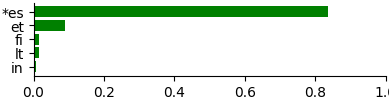
\includegraphics{img/infer/bar-lang-placeholder}}}
    %\caption{test}
%\end{figure}

Our UnicodeCNN model correctly identifies that the previous tweet was sent from Spain,
as shown in the following graph:

\noindent%% Creator: Matplotlib, PGF backend
%%
%% To include the figure in your LaTeX document, write
%%   \input{<filename>.pgf}
%%
%% Make sure the required packages are loaded in your preamble
%%   \usepackage{pgf}
%%
%% Figures using additional raster images can only be included by \input if
%% they are in the same directory as the main LaTeX file. For loading figures
%% from other directories you can use the `import` package
%%   \usepackage{import}
%% and then include the figures with
%%   \import{<path to file>}{<filename>.pgf}
%%
%% Matplotlib used the following preamble
%%   \usepackage{fontspec}
%%
\begingroup%
\makeatletter%
\begin{pgfpicture}%
\pgfpathrectangle{\pgfpointorigin}{\pgfqpoint{3.500000in}{0.700000in}}%
\pgfusepath{use as bounding box, clip}%
\begin{pgfscope}%
\pgfsetbuttcap%
\pgfsetmiterjoin%
\definecolor{currentfill}{rgb}{1.000000,1.000000,1.000000}%
\pgfsetfillcolor{currentfill}%
\pgfsetlinewidth{0.000000pt}%
\definecolor{currentstroke}{rgb}{1.000000,1.000000,1.000000}%
\pgfsetstrokecolor{currentstroke}%
\pgfsetdash{}{0pt}%
\pgfpathmoveto{\pgfqpoint{0.000000in}{0.000000in}}%
\pgfpathlineto{\pgfqpoint{3.500000in}{0.000000in}}%
\pgfpathlineto{\pgfqpoint{3.500000in}{0.700000in}}%
\pgfpathlineto{\pgfqpoint{0.000000in}{0.700000in}}%
\pgfpathclose%
\pgfusepath{fill}%
\end{pgfscope}%
\begin{pgfscope}%
\pgfsetbuttcap%
\pgfsetmiterjoin%
\definecolor{currentfill}{rgb}{1.000000,1.000000,1.000000}%
\pgfsetfillcolor{currentfill}%
\pgfsetlinewidth{0.000000pt}%
\definecolor{currentstroke}{rgb}{0.000000,0.000000,0.000000}%
\pgfsetstrokecolor{currentstroke}%
\pgfsetstrokeopacity{0.000000}%
\pgfsetdash{}{0pt}%
\pgfpathmoveto{\pgfqpoint{1.050000in}{0.245000in}}%
\pgfpathlineto{\pgfqpoint{3.150000in}{0.245000in}}%
\pgfpathlineto{\pgfqpoint{3.150000in}{0.616000in}}%
\pgfpathlineto{\pgfqpoint{1.050000in}{0.616000in}}%
\pgfpathclose%
\pgfusepath{fill}%
\end{pgfscope}%
\begin{pgfscope}%
\pgfpathrectangle{\pgfqpoint{1.050000in}{0.245000in}}{\pgfqpoint{2.100000in}{0.371000in}} %
\pgfusepath{clip}%
\pgfsetbuttcap%
\pgfsetmiterjoin%
\definecolor{currentfill}{rgb}{0.000000,0.501961,0.000000}%
\pgfsetfillcolor{currentfill}%
\pgfsetlinewidth{0.000000pt}%
\definecolor{currentstroke}{rgb}{0.000000,0.000000,0.000000}%
\pgfsetstrokecolor{currentstroke}%
\pgfsetstrokeopacity{0.000000}%
\pgfsetdash{}{0pt}%
\pgfpathmoveto{\pgfqpoint{1.050000in}{0.599136in}}%
\pgfpathlineto{\pgfqpoint{3.038161in}{0.599136in}}%
\pgfpathlineto{\pgfqpoint{3.038161in}{0.502773in}}%
\pgfpathlineto{\pgfqpoint{1.050000in}{0.502773in}}%
\pgfpathclose%
\pgfusepath{fill}%
\end{pgfscope}%
\begin{pgfscope}%
\pgfpathrectangle{\pgfqpoint{1.050000in}{0.245000in}}{\pgfqpoint{2.100000in}{0.371000in}} %
\pgfusepath{clip}%
\pgfsetbuttcap%
\pgfsetmiterjoin%
\definecolor{currentfill}{rgb}{0.000000,0.501961,0.000000}%
\pgfsetfillcolor{currentfill}%
\pgfsetlinewidth{0.000000pt}%
\definecolor{currentstroke}{rgb}{0.000000,0.000000,0.000000}%
\pgfsetstrokecolor{currentstroke}%
\pgfsetstrokeopacity{0.000000}%
\pgfsetdash{}{0pt}%
\pgfpathmoveto{\pgfqpoint{1.050000in}{0.478682in}}%
\pgfpathlineto{\pgfqpoint{1.080903in}{0.478682in}}%
\pgfpathlineto{\pgfqpoint{1.080903in}{0.382318in}}%
\pgfpathlineto{\pgfqpoint{1.050000in}{0.382318in}}%
\pgfpathclose%
\pgfusepath{fill}%
\end{pgfscope}%
\begin{pgfscope}%
\pgfpathrectangle{\pgfqpoint{1.050000in}{0.245000in}}{\pgfqpoint{2.100000in}{0.371000in}} %
\pgfusepath{clip}%
\pgfsetbuttcap%
\pgfsetmiterjoin%
\definecolor{currentfill}{rgb}{0.000000,0.501961,0.000000}%
\pgfsetfillcolor{currentfill}%
\pgfsetlinewidth{0.000000pt}%
\definecolor{currentstroke}{rgb}{0.000000,0.000000,0.000000}%
\pgfsetstrokecolor{currentstroke}%
\pgfsetstrokeopacity{0.000000}%
\pgfsetdash{}{0pt}%
\pgfpathmoveto{\pgfqpoint{1.050000in}{0.358227in}}%
\pgfpathlineto{\pgfqpoint{1.068129in}{0.358227in}}%
\pgfpathlineto{\pgfqpoint{1.068129in}{0.261864in}}%
\pgfpathlineto{\pgfqpoint{1.050000in}{0.261864in}}%
\pgfpathclose%
\pgfusepath{fill}%
\end{pgfscope}%
\begin{pgfscope}%
\pgfsetbuttcap%
\pgfsetroundjoin%
\definecolor{currentfill}{rgb}{0.000000,0.000000,0.000000}%
\pgfsetfillcolor{currentfill}%
\pgfsetlinewidth{0.803000pt}%
\definecolor{currentstroke}{rgb}{0.000000,0.000000,0.000000}%
\pgfsetstrokecolor{currentstroke}%
\pgfsetdash{}{0pt}%
\pgfsys@defobject{currentmarker}{\pgfqpoint{0.000000in}{-0.048611in}}{\pgfqpoint{0.000000in}{0.000000in}}{%
\pgfpathmoveto{\pgfqpoint{0.000000in}{0.000000in}}%
\pgfpathlineto{\pgfqpoint{0.000000in}{-0.048611in}}%
\pgfusepath{stroke,fill}%
}%
\begin{pgfscope}%
\pgfsys@transformshift{1.050000in}{0.245000in}%
\pgfsys@useobject{currentmarker}{}%
\end{pgfscope}%
\end{pgfscope}%
\begin{pgfscope}%
\pgftext[x=1.050000in,y=0.147778in,,top]{\sffamily\fontsize{8.000000}{9.600000}\selectfont 0.0}%
\end{pgfscope}%
\begin{pgfscope}%
\pgfsetbuttcap%
\pgfsetroundjoin%
\definecolor{currentfill}{rgb}{0.000000,0.000000,0.000000}%
\pgfsetfillcolor{currentfill}%
\pgfsetlinewidth{0.803000pt}%
\definecolor{currentstroke}{rgb}{0.000000,0.000000,0.000000}%
\pgfsetstrokecolor{currentstroke}%
\pgfsetdash{}{0pt}%
\pgfsys@defobject{currentmarker}{\pgfqpoint{0.000000in}{-0.048611in}}{\pgfqpoint{0.000000in}{0.000000in}}{%
\pgfpathmoveto{\pgfqpoint{0.000000in}{0.000000in}}%
\pgfpathlineto{\pgfqpoint{0.000000in}{-0.048611in}}%
\pgfusepath{stroke,fill}%
}%
\begin{pgfscope}%
\pgfsys@transformshift{1.470000in}{0.245000in}%
\pgfsys@useobject{currentmarker}{}%
\end{pgfscope}%
\end{pgfscope}%
\begin{pgfscope}%
\pgftext[x=1.470000in,y=0.147778in,,top]{\sffamily\fontsize{8.000000}{9.600000}\selectfont 0.2}%
\end{pgfscope}%
\begin{pgfscope}%
\pgfsetbuttcap%
\pgfsetroundjoin%
\definecolor{currentfill}{rgb}{0.000000,0.000000,0.000000}%
\pgfsetfillcolor{currentfill}%
\pgfsetlinewidth{0.803000pt}%
\definecolor{currentstroke}{rgb}{0.000000,0.000000,0.000000}%
\pgfsetstrokecolor{currentstroke}%
\pgfsetdash{}{0pt}%
\pgfsys@defobject{currentmarker}{\pgfqpoint{0.000000in}{-0.048611in}}{\pgfqpoint{0.000000in}{0.000000in}}{%
\pgfpathmoveto{\pgfqpoint{0.000000in}{0.000000in}}%
\pgfpathlineto{\pgfqpoint{0.000000in}{-0.048611in}}%
\pgfusepath{stroke,fill}%
}%
\begin{pgfscope}%
\pgfsys@transformshift{1.890000in}{0.245000in}%
\pgfsys@useobject{currentmarker}{}%
\end{pgfscope}%
\end{pgfscope}%
\begin{pgfscope}%
\pgftext[x=1.890000in,y=0.147778in,,top]{\sffamily\fontsize{8.000000}{9.600000}\selectfont 0.4}%
\end{pgfscope}%
\begin{pgfscope}%
\pgfsetbuttcap%
\pgfsetroundjoin%
\definecolor{currentfill}{rgb}{0.000000,0.000000,0.000000}%
\pgfsetfillcolor{currentfill}%
\pgfsetlinewidth{0.803000pt}%
\definecolor{currentstroke}{rgb}{0.000000,0.000000,0.000000}%
\pgfsetstrokecolor{currentstroke}%
\pgfsetdash{}{0pt}%
\pgfsys@defobject{currentmarker}{\pgfqpoint{0.000000in}{-0.048611in}}{\pgfqpoint{0.000000in}{0.000000in}}{%
\pgfpathmoveto{\pgfqpoint{0.000000in}{0.000000in}}%
\pgfpathlineto{\pgfqpoint{0.000000in}{-0.048611in}}%
\pgfusepath{stroke,fill}%
}%
\begin{pgfscope}%
\pgfsys@transformshift{2.310000in}{0.245000in}%
\pgfsys@useobject{currentmarker}{}%
\end{pgfscope}%
\end{pgfscope}%
\begin{pgfscope}%
\pgftext[x=2.310000in,y=0.147778in,,top]{\sffamily\fontsize{8.000000}{9.600000}\selectfont 0.6}%
\end{pgfscope}%
\begin{pgfscope}%
\pgfsetbuttcap%
\pgfsetroundjoin%
\definecolor{currentfill}{rgb}{0.000000,0.000000,0.000000}%
\pgfsetfillcolor{currentfill}%
\pgfsetlinewidth{0.803000pt}%
\definecolor{currentstroke}{rgb}{0.000000,0.000000,0.000000}%
\pgfsetstrokecolor{currentstroke}%
\pgfsetdash{}{0pt}%
\pgfsys@defobject{currentmarker}{\pgfqpoint{0.000000in}{-0.048611in}}{\pgfqpoint{0.000000in}{0.000000in}}{%
\pgfpathmoveto{\pgfqpoint{0.000000in}{0.000000in}}%
\pgfpathlineto{\pgfqpoint{0.000000in}{-0.048611in}}%
\pgfusepath{stroke,fill}%
}%
\begin{pgfscope}%
\pgfsys@transformshift{2.730000in}{0.245000in}%
\pgfsys@useobject{currentmarker}{}%
\end{pgfscope}%
\end{pgfscope}%
\begin{pgfscope}%
\pgftext[x=2.730000in,y=0.147778in,,top]{\sffamily\fontsize{8.000000}{9.600000}\selectfont 0.8}%
\end{pgfscope}%
\begin{pgfscope}%
\pgfsetbuttcap%
\pgfsetroundjoin%
\definecolor{currentfill}{rgb}{0.000000,0.000000,0.000000}%
\pgfsetfillcolor{currentfill}%
\pgfsetlinewidth{0.803000pt}%
\definecolor{currentstroke}{rgb}{0.000000,0.000000,0.000000}%
\pgfsetstrokecolor{currentstroke}%
\pgfsetdash{}{0pt}%
\pgfsys@defobject{currentmarker}{\pgfqpoint{0.000000in}{-0.048611in}}{\pgfqpoint{0.000000in}{0.000000in}}{%
\pgfpathmoveto{\pgfqpoint{0.000000in}{0.000000in}}%
\pgfpathlineto{\pgfqpoint{0.000000in}{-0.048611in}}%
\pgfusepath{stroke,fill}%
}%
\begin{pgfscope}%
\pgfsys@transformshift{3.150000in}{0.245000in}%
\pgfsys@useobject{currentmarker}{}%
\end{pgfscope}%
\end{pgfscope}%
\begin{pgfscope}%
\pgftext[x=3.150000in,y=0.147778in,,top]{\sffamily\fontsize{8.000000}{9.600000}\selectfont 1.0}%
\end{pgfscope}%
\begin{pgfscope}%
\pgfsetbuttcap%
\pgfsetroundjoin%
\definecolor{currentfill}{rgb}{0.000000,0.000000,0.000000}%
\pgfsetfillcolor{currentfill}%
\pgfsetlinewidth{0.803000pt}%
\definecolor{currentstroke}{rgb}{0.000000,0.000000,0.000000}%
\pgfsetstrokecolor{currentstroke}%
\pgfsetdash{}{0pt}%
\pgfsys@defobject{currentmarker}{\pgfqpoint{-0.048611in}{0.000000in}}{\pgfqpoint{0.000000in}{0.000000in}}{%
\pgfpathmoveto{\pgfqpoint{0.000000in}{0.000000in}}%
\pgfpathlineto{\pgfqpoint{-0.048611in}{0.000000in}}%
\pgfusepath{stroke,fill}%
}%
\begin{pgfscope}%
\pgfsys@transformshift{1.050000in}{0.550955in}%
\pgfsys@useobject{currentmarker}{}%
\end{pgfscope}%
\end{pgfscope}%
\begin{pgfscope}%
\pgftext[x=0.608333in,y=0.512399in,left,base]{\sffamily\fontsize{8.000000}{9.600000}\selectfont Kuwait}%
\end{pgfscope}%
\begin{pgfscope}%
\pgfsetbuttcap%
\pgfsetroundjoin%
\definecolor{currentfill}{rgb}{0.000000,0.000000,0.000000}%
\pgfsetfillcolor{currentfill}%
\pgfsetlinewidth{0.803000pt}%
\definecolor{currentstroke}{rgb}{0.000000,0.000000,0.000000}%
\pgfsetstrokecolor{currentstroke}%
\pgfsetdash{}{0pt}%
\pgfsys@defobject{currentmarker}{\pgfqpoint{-0.048611in}{0.000000in}}{\pgfqpoint{0.000000in}{0.000000in}}{%
\pgfpathmoveto{\pgfqpoint{0.000000in}{0.000000in}}%
\pgfpathlineto{\pgfqpoint{-0.048611in}{0.000000in}}%
\pgfusepath{stroke,fill}%
}%
\begin{pgfscope}%
\pgfsys@transformshift{1.050000in}{0.430500in}%
\pgfsys@useobject{currentmarker}{}%
\end{pgfscope}%
\end{pgfscope}%
\begin{pgfscope}%
\pgftext[x=0.319667in,y=0.391944in,left,base]{\sffamily\fontsize{8.000000}{9.600000}\selectfont Saudi Arabia}%
\end{pgfscope}%
\begin{pgfscope}%
\pgfsetbuttcap%
\pgfsetroundjoin%
\definecolor{currentfill}{rgb}{0.000000,0.000000,0.000000}%
\pgfsetfillcolor{currentfill}%
\pgfsetlinewidth{0.803000pt}%
\definecolor{currentstroke}{rgb}{0.000000,0.000000,0.000000}%
\pgfsetstrokecolor{currentstroke}%
\pgfsetdash{}{0pt}%
\pgfsys@defobject{currentmarker}{\pgfqpoint{-0.048611in}{0.000000in}}{\pgfqpoint{0.000000in}{0.000000in}}{%
\pgfpathmoveto{\pgfqpoint{0.000000in}{0.000000in}}%
\pgfpathlineto{\pgfqpoint{-0.048611in}{0.000000in}}%
\pgfusepath{stroke,fill}%
}%
\begin{pgfscope}%
\pgfsys@transformshift{1.050000in}{0.310045in}%
\pgfsys@useobject{currentmarker}{}%
\end{pgfscope}%
\end{pgfscope}%
\begin{pgfscope}%
\pgftext[x=0.664889in,y=0.271657in,left,base]{\sffamily\fontsize{8.000000}{9.600000}\selectfont Egypt}%
\end{pgfscope}%
\begin{pgfscope}%
\pgfsetrectcap%
\pgfsetmiterjoin%
\pgfsetlinewidth{0.803000pt}%
\definecolor{currentstroke}{rgb}{0.000000,0.000000,0.000000}%
\pgfsetstrokecolor{currentstroke}%
\pgfsetdash{}{0pt}%
\pgfpathmoveto{\pgfqpoint{1.050000in}{0.245000in}}%
\pgfpathlineto{\pgfqpoint{1.050000in}{0.616000in}}%
\pgfusepath{stroke}%
\end{pgfscope}%
\begin{pgfscope}%
\pgfsetrectcap%
\pgfsetmiterjoin%
\pgfsetlinewidth{0.803000pt}%
\definecolor{currentstroke}{rgb}{0.000000,0.000000,0.000000}%
\pgfsetstrokecolor{currentstroke}%
\pgfsetdash{}{0pt}%
\pgfpathmoveto{\pgfqpoint{1.050000in}{0.245000in}}%
\pgfpathlineto{\pgfqpoint{3.150000in}{0.245000in}}%
\pgfusepath{stroke}%
\end{pgfscope}%
\end{pgfpicture}%
\makeatother%
\endgroup%


\noindent
%To demonstrate that our model is able to distinguish between the words \str{pod\'eis} and \str{pueden},
%we create two artificial tweets
%\begin{figure}[H]
    %\centering
    %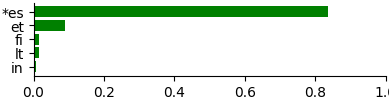
\includegraphics[width=0.45\textwidth]{img/infer/bar-lang-placeholder}
%\end{figure}
%And running the same model on the word \str{pueden} gives
If we were to instead replace the word \str{pod\'eis} in the tweet above by the word \str{pueden},
then our model predicts the following countries

\noindent%% Creator: Matplotlib, PGF backend
%%
%% To include the figure in your LaTeX document, write
%%   \input{<filename>.pgf}
%%
%% Make sure the required packages are loaded in your preamble
%%   \usepackage{pgf}
%%
%% Figures using additional raster images can only be included by \input if
%% they are in the same directory as the main LaTeX file. For loading figures
%% from other directories you can use the `import` package
%%   \usepackage{import}
%% and then include the figures with
%%   \import{<path to file>}{<filename>.pgf}
%%
%% Matplotlib used the following preamble
%%   \usepackage{fontspec}
%%
\begingroup%
\makeatletter%
\begin{pgfpicture}%
\pgfpathrectangle{\pgfpointorigin}{\pgfqpoint{3.500000in}{0.700000in}}%
\pgfusepath{use as bounding box, clip}%
\begin{pgfscope}%
\pgfsetbuttcap%
\pgfsetmiterjoin%
\definecolor{currentfill}{rgb}{1.000000,1.000000,1.000000}%
\pgfsetfillcolor{currentfill}%
\pgfsetlinewidth{0.000000pt}%
\definecolor{currentstroke}{rgb}{1.000000,1.000000,1.000000}%
\pgfsetstrokecolor{currentstroke}%
\pgfsetdash{}{0pt}%
\pgfpathmoveto{\pgfqpoint{0.000000in}{0.000000in}}%
\pgfpathlineto{\pgfqpoint{3.500000in}{0.000000in}}%
\pgfpathlineto{\pgfqpoint{3.500000in}{0.700000in}}%
\pgfpathlineto{\pgfqpoint{0.000000in}{0.700000in}}%
\pgfpathclose%
\pgfusepath{fill}%
\end{pgfscope}%
\begin{pgfscope}%
\pgfsetbuttcap%
\pgfsetmiterjoin%
\definecolor{currentfill}{rgb}{1.000000,1.000000,1.000000}%
\pgfsetfillcolor{currentfill}%
\pgfsetlinewidth{0.000000pt}%
\definecolor{currentstroke}{rgb}{0.000000,0.000000,0.000000}%
\pgfsetstrokecolor{currentstroke}%
\pgfsetstrokeopacity{0.000000}%
\pgfsetdash{}{0pt}%
\pgfpathmoveto{\pgfqpoint{1.050000in}{0.245000in}}%
\pgfpathlineto{\pgfqpoint{3.150000in}{0.245000in}}%
\pgfpathlineto{\pgfqpoint{3.150000in}{0.616000in}}%
\pgfpathlineto{\pgfqpoint{1.050000in}{0.616000in}}%
\pgfpathclose%
\pgfusepath{fill}%
\end{pgfscope}%
\begin{pgfscope}%
\pgfpathrectangle{\pgfqpoint{1.050000in}{0.245000in}}{\pgfqpoint{2.100000in}{0.371000in}} %
\pgfusepath{clip}%
\pgfsetbuttcap%
\pgfsetmiterjoin%
\definecolor{currentfill}{rgb}{0.000000,0.501961,0.000000}%
\pgfsetfillcolor{currentfill}%
\pgfsetlinewidth{0.000000pt}%
\definecolor{currentstroke}{rgb}{0.000000,0.000000,0.000000}%
\pgfsetstrokecolor{currentstroke}%
\pgfsetstrokeopacity{0.000000}%
\pgfsetdash{}{0pt}%
\pgfpathmoveto{\pgfqpoint{1.050000in}{0.599136in}}%
\pgfpathlineto{\pgfqpoint{3.038161in}{0.599136in}}%
\pgfpathlineto{\pgfqpoint{3.038161in}{0.502773in}}%
\pgfpathlineto{\pgfqpoint{1.050000in}{0.502773in}}%
\pgfpathclose%
\pgfusepath{fill}%
\end{pgfscope}%
\begin{pgfscope}%
\pgfpathrectangle{\pgfqpoint{1.050000in}{0.245000in}}{\pgfqpoint{2.100000in}{0.371000in}} %
\pgfusepath{clip}%
\pgfsetbuttcap%
\pgfsetmiterjoin%
\definecolor{currentfill}{rgb}{0.000000,0.501961,0.000000}%
\pgfsetfillcolor{currentfill}%
\pgfsetlinewidth{0.000000pt}%
\definecolor{currentstroke}{rgb}{0.000000,0.000000,0.000000}%
\pgfsetstrokecolor{currentstroke}%
\pgfsetstrokeopacity{0.000000}%
\pgfsetdash{}{0pt}%
\pgfpathmoveto{\pgfqpoint{1.050000in}{0.478682in}}%
\pgfpathlineto{\pgfqpoint{1.080903in}{0.478682in}}%
\pgfpathlineto{\pgfqpoint{1.080903in}{0.382318in}}%
\pgfpathlineto{\pgfqpoint{1.050000in}{0.382318in}}%
\pgfpathclose%
\pgfusepath{fill}%
\end{pgfscope}%
\begin{pgfscope}%
\pgfpathrectangle{\pgfqpoint{1.050000in}{0.245000in}}{\pgfqpoint{2.100000in}{0.371000in}} %
\pgfusepath{clip}%
\pgfsetbuttcap%
\pgfsetmiterjoin%
\definecolor{currentfill}{rgb}{0.000000,0.501961,0.000000}%
\pgfsetfillcolor{currentfill}%
\pgfsetlinewidth{0.000000pt}%
\definecolor{currentstroke}{rgb}{0.000000,0.000000,0.000000}%
\pgfsetstrokecolor{currentstroke}%
\pgfsetstrokeopacity{0.000000}%
\pgfsetdash{}{0pt}%
\pgfpathmoveto{\pgfqpoint{1.050000in}{0.358227in}}%
\pgfpathlineto{\pgfqpoint{1.068129in}{0.358227in}}%
\pgfpathlineto{\pgfqpoint{1.068129in}{0.261864in}}%
\pgfpathlineto{\pgfqpoint{1.050000in}{0.261864in}}%
\pgfpathclose%
\pgfusepath{fill}%
\end{pgfscope}%
\begin{pgfscope}%
\pgfsetbuttcap%
\pgfsetroundjoin%
\definecolor{currentfill}{rgb}{0.000000,0.000000,0.000000}%
\pgfsetfillcolor{currentfill}%
\pgfsetlinewidth{0.803000pt}%
\definecolor{currentstroke}{rgb}{0.000000,0.000000,0.000000}%
\pgfsetstrokecolor{currentstroke}%
\pgfsetdash{}{0pt}%
\pgfsys@defobject{currentmarker}{\pgfqpoint{0.000000in}{-0.048611in}}{\pgfqpoint{0.000000in}{0.000000in}}{%
\pgfpathmoveto{\pgfqpoint{0.000000in}{0.000000in}}%
\pgfpathlineto{\pgfqpoint{0.000000in}{-0.048611in}}%
\pgfusepath{stroke,fill}%
}%
\begin{pgfscope}%
\pgfsys@transformshift{1.050000in}{0.245000in}%
\pgfsys@useobject{currentmarker}{}%
\end{pgfscope}%
\end{pgfscope}%
\begin{pgfscope}%
\pgftext[x=1.050000in,y=0.147778in,,top]{\sffamily\fontsize{8.000000}{9.600000}\selectfont 0.0}%
\end{pgfscope}%
\begin{pgfscope}%
\pgfsetbuttcap%
\pgfsetroundjoin%
\definecolor{currentfill}{rgb}{0.000000,0.000000,0.000000}%
\pgfsetfillcolor{currentfill}%
\pgfsetlinewidth{0.803000pt}%
\definecolor{currentstroke}{rgb}{0.000000,0.000000,0.000000}%
\pgfsetstrokecolor{currentstroke}%
\pgfsetdash{}{0pt}%
\pgfsys@defobject{currentmarker}{\pgfqpoint{0.000000in}{-0.048611in}}{\pgfqpoint{0.000000in}{0.000000in}}{%
\pgfpathmoveto{\pgfqpoint{0.000000in}{0.000000in}}%
\pgfpathlineto{\pgfqpoint{0.000000in}{-0.048611in}}%
\pgfusepath{stroke,fill}%
}%
\begin{pgfscope}%
\pgfsys@transformshift{1.470000in}{0.245000in}%
\pgfsys@useobject{currentmarker}{}%
\end{pgfscope}%
\end{pgfscope}%
\begin{pgfscope}%
\pgftext[x=1.470000in,y=0.147778in,,top]{\sffamily\fontsize{8.000000}{9.600000}\selectfont 0.2}%
\end{pgfscope}%
\begin{pgfscope}%
\pgfsetbuttcap%
\pgfsetroundjoin%
\definecolor{currentfill}{rgb}{0.000000,0.000000,0.000000}%
\pgfsetfillcolor{currentfill}%
\pgfsetlinewidth{0.803000pt}%
\definecolor{currentstroke}{rgb}{0.000000,0.000000,0.000000}%
\pgfsetstrokecolor{currentstroke}%
\pgfsetdash{}{0pt}%
\pgfsys@defobject{currentmarker}{\pgfqpoint{0.000000in}{-0.048611in}}{\pgfqpoint{0.000000in}{0.000000in}}{%
\pgfpathmoveto{\pgfqpoint{0.000000in}{0.000000in}}%
\pgfpathlineto{\pgfqpoint{0.000000in}{-0.048611in}}%
\pgfusepath{stroke,fill}%
}%
\begin{pgfscope}%
\pgfsys@transformshift{1.890000in}{0.245000in}%
\pgfsys@useobject{currentmarker}{}%
\end{pgfscope}%
\end{pgfscope}%
\begin{pgfscope}%
\pgftext[x=1.890000in,y=0.147778in,,top]{\sffamily\fontsize{8.000000}{9.600000}\selectfont 0.4}%
\end{pgfscope}%
\begin{pgfscope}%
\pgfsetbuttcap%
\pgfsetroundjoin%
\definecolor{currentfill}{rgb}{0.000000,0.000000,0.000000}%
\pgfsetfillcolor{currentfill}%
\pgfsetlinewidth{0.803000pt}%
\definecolor{currentstroke}{rgb}{0.000000,0.000000,0.000000}%
\pgfsetstrokecolor{currentstroke}%
\pgfsetdash{}{0pt}%
\pgfsys@defobject{currentmarker}{\pgfqpoint{0.000000in}{-0.048611in}}{\pgfqpoint{0.000000in}{0.000000in}}{%
\pgfpathmoveto{\pgfqpoint{0.000000in}{0.000000in}}%
\pgfpathlineto{\pgfqpoint{0.000000in}{-0.048611in}}%
\pgfusepath{stroke,fill}%
}%
\begin{pgfscope}%
\pgfsys@transformshift{2.310000in}{0.245000in}%
\pgfsys@useobject{currentmarker}{}%
\end{pgfscope}%
\end{pgfscope}%
\begin{pgfscope}%
\pgftext[x=2.310000in,y=0.147778in,,top]{\sffamily\fontsize{8.000000}{9.600000}\selectfont 0.6}%
\end{pgfscope}%
\begin{pgfscope}%
\pgfsetbuttcap%
\pgfsetroundjoin%
\definecolor{currentfill}{rgb}{0.000000,0.000000,0.000000}%
\pgfsetfillcolor{currentfill}%
\pgfsetlinewidth{0.803000pt}%
\definecolor{currentstroke}{rgb}{0.000000,0.000000,0.000000}%
\pgfsetstrokecolor{currentstroke}%
\pgfsetdash{}{0pt}%
\pgfsys@defobject{currentmarker}{\pgfqpoint{0.000000in}{-0.048611in}}{\pgfqpoint{0.000000in}{0.000000in}}{%
\pgfpathmoveto{\pgfqpoint{0.000000in}{0.000000in}}%
\pgfpathlineto{\pgfqpoint{0.000000in}{-0.048611in}}%
\pgfusepath{stroke,fill}%
}%
\begin{pgfscope}%
\pgfsys@transformshift{2.730000in}{0.245000in}%
\pgfsys@useobject{currentmarker}{}%
\end{pgfscope}%
\end{pgfscope}%
\begin{pgfscope}%
\pgftext[x=2.730000in,y=0.147778in,,top]{\sffamily\fontsize{8.000000}{9.600000}\selectfont 0.8}%
\end{pgfscope}%
\begin{pgfscope}%
\pgfsetbuttcap%
\pgfsetroundjoin%
\definecolor{currentfill}{rgb}{0.000000,0.000000,0.000000}%
\pgfsetfillcolor{currentfill}%
\pgfsetlinewidth{0.803000pt}%
\definecolor{currentstroke}{rgb}{0.000000,0.000000,0.000000}%
\pgfsetstrokecolor{currentstroke}%
\pgfsetdash{}{0pt}%
\pgfsys@defobject{currentmarker}{\pgfqpoint{0.000000in}{-0.048611in}}{\pgfqpoint{0.000000in}{0.000000in}}{%
\pgfpathmoveto{\pgfqpoint{0.000000in}{0.000000in}}%
\pgfpathlineto{\pgfqpoint{0.000000in}{-0.048611in}}%
\pgfusepath{stroke,fill}%
}%
\begin{pgfscope}%
\pgfsys@transformshift{3.150000in}{0.245000in}%
\pgfsys@useobject{currentmarker}{}%
\end{pgfscope}%
\end{pgfscope}%
\begin{pgfscope}%
\pgftext[x=3.150000in,y=0.147778in,,top]{\sffamily\fontsize{8.000000}{9.600000}\selectfont 1.0}%
\end{pgfscope}%
\begin{pgfscope}%
\pgfsetbuttcap%
\pgfsetroundjoin%
\definecolor{currentfill}{rgb}{0.000000,0.000000,0.000000}%
\pgfsetfillcolor{currentfill}%
\pgfsetlinewidth{0.803000pt}%
\definecolor{currentstroke}{rgb}{0.000000,0.000000,0.000000}%
\pgfsetstrokecolor{currentstroke}%
\pgfsetdash{}{0pt}%
\pgfsys@defobject{currentmarker}{\pgfqpoint{-0.048611in}{0.000000in}}{\pgfqpoint{0.000000in}{0.000000in}}{%
\pgfpathmoveto{\pgfqpoint{0.000000in}{0.000000in}}%
\pgfpathlineto{\pgfqpoint{-0.048611in}{0.000000in}}%
\pgfusepath{stroke,fill}%
}%
\begin{pgfscope}%
\pgfsys@transformshift{1.050000in}{0.550955in}%
\pgfsys@useobject{currentmarker}{}%
\end{pgfscope}%
\end{pgfscope}%
\begin{pgfscope}%
\pgftext[x=0.608333in,y=0.512399in,left,base]{\sffamily\fontsize{8.000000}{9.600000}\selectfont Kuwait}%
\end{pgfscope}%
\begin{pgfscope}%
\pgfsetbuttcap%
\pgfsetroundjoin%
\definecolor{currentfill}{rgb}{0.000000,0.000000,0.000000}%
\pgfsetfillcolor{currentfill}%
\pgfsetlinewidth{0.803000pt}%
\definecolor{currentstroke}{rgb}{0.000000,0.000000,0.000000}%
\pgfsetstrokecolor{currentstroke}%
\pgfsetdash{}{0pt}%
\pgfsys@defobject{currentmarker}{\pgfqpoint{-0.048611in}{0.000000in}}{\pgfqpoint{0.000000in}{0.000000in}}{%
\pgfpathmoveto{\pgfqpoint{0.000000in}{0.000000in}}%
\pgfpathlineto{\pgfqpoint{-0.048611in}{0.000000in}}%
\pgfusepath{stroke,fill}%
}%
\begin{pgfscope}%
\pgfsys@transformshift{1.050000in}{0.430500in}%
\pgfsys@useobject{currentmarker}{}%
\end{pgfscope}%
\end{pgfscope}%
\begin{pgfscope}%
\pgftext[x=0.319667in,y=0.391944in,left,base]{\sffamily\fontsize{8.000000}{9.600000}\selectfont Saudi Arabia}%
\end{pgfscope}%
\begin{pgfscope}%
\pgfsetbuttcap%
\pgfsetroundjoin%
\definecolor{currentfill}{rgb}{0.000000,0.000000,0.000000}%
\pgfsetfillcolor{currentfill}%
\pgfsetlinewidth{0.803000pt}%
\definecolor{currentstroke}{rgb}{0.000000,0.000000,0.000000}%
\pgfsetstrokecolor{currentstroke}%
\pgfsetdash{}{0pt}%
\pgfsys@defobject{currentmarker}{\pgfqpoint{-0.048611in}{0.000000in}}{\pgfqpoint{0.000000in}{0.000000in}}{%
\pgfpathmoveto{\pgfqpoint{0.000000in}{0.000000in}}%
\pgfpathlineto{\pgfqpoint{-0.048611in}{0.000000in}}%
\pgfusepath{stroke,fill}%
}%
\begin{pgfscope}%
\pgfsys@transformshift{1.050000in}{0.310045in}%
\pgfsys@useobject{currentmarker}{}%
\end{pgfscope}%
\end{pgfscope}%
\begin{pgfscope}%
\pgftext[x=0.664889in,y=0.271657in,left,base]{\sffamily\fontsize{8.000000}{9.600000}\selectfont Egypt}%
\end{pgfscope}%
\begin{pgfscope}%
\pgfsetrectcap%
\pgfsetmiterjoin%
\pgfsetlinewidth{0.803000pt}%
\definecolor{currentstroke}{rgb}{0.000000,0.000000,0.000000}%
\pgfsetstrokecolor{currentstroke}%
\pgfsetdash{}{0pt}%
\pgfpathmoveto{\pgfqpoint{1.050000in}{0.245000in}}%
\pgfpathlineto{\pgfqpoint{1.050000in}{0.616000in}}%
\pgfusepath{stroke}%
\end{pgfscope}%
\begin{pgfscope}%
\pgfsetrectcap%
\pgfsetmiterjoin%
\pgfsetlinewidth{0.803000pt}%
\definecolor{currentstroke}{rgb}{0.000000,0.000000,0.000000}%
\pgfsetstrokecolor{currentstroke}%
\pgfsetdash{}{0pt}%
\pgfpathmoveto{\pgfqpoint{1.050000in}{0.245000in}}%
\pgfpathlineto{\pgfqpoint{3.150000in}{0.245000in}}%
\pgfusepath{stroke}%
\end{pgfscope}%
\end{pgfpicture}%
\makeatother%
\endgroup%


\noindent
Remarkably, these patterns generalize to misspellings and words not present in the original training set.
For example, the Spanish word \str{fallec\'eis} is another verb conjugated in the Castilian vosotros form.
This word is not present in our training set,
yet if we replace the word \str{pod\'eis} by \str{fallec\'eis} the model still predicts that the tweet was sent from Spain.

\noindent%% Creator: Matplotlib, PGF backend
%%
%% To include the figure in your LaTeX document, write
%%   \input{<filename>.pgf}
%%
%% Make sure the required packages are loaded in your preamble
%%   \usepackage{pgf}
%%
%% Figures using additional raster images can only be included by \input if
%% they are in the same directory as the main LaTeX file. For loading figures
%% from other directories you can use the `import` package
%%   \usepackage{import}
%% and then include the figures with
%%   \import{<path to file>}{<filename>.pgf}
%%
%% Matplotlib used the following preamble
%%   \usepackage{fontspec}
%%
\begingroup%
\makeatletter%
\begin{pgfpicture}%
\pgfpathrectangle{\pgfpointorigin}{\pgfqpoint{3.500000in}{0.700000in}}%
\pgfusepath{use as bounding box, clip}%
\begin{pgfscope}%
\pgfsetbuttcap%
\pgfsetmiterjoin%
\definecolor{currentfill}{rgb}{1.000000,1.000000,1.000000}%
\pgfsetfillcolor{currentfill}%
\pgfsetlinewidth{0.000000pt}%
\definecolor{currentstroke}{rgb}{1.000000,1.000000,1.000000}%
\pgfsetstrokecolor{currentstroke}%
\pgfsetdash{}{0pt}%
\pgfpathmoveto{\pgfqpoint{0.000000in}{0.000000in}}%
\pgfpathlineto{\pgfqpoint{3.500000in}{0.000000in}}%
\pgfpathlineto{\pgfqpoint{3.500000in}{0.700000in}}%
\pgfpathlineto{\pgfqpoint{0.000000in}{0.700000in}}%
\pgfpathclose%
\pgfusepath{fill}%
\end{pgfscope}%
\begin{pgfscope}%
\pgfsetbuttcap%
\pgfsetmiterjoin%
\definecolor{currentfill}{rgb}{1.000000,1.000000,1.000000}%
\pgfsetfillcolor{currentfill}%
\pgfsetlinewidth{0.000000pt}%
\definecolor{currentstroke}{rgb}{0.000000,0.000000,0.000000}%
\pgfsetstrokecolor{currentstroke}%
\pgfsetstrokeopacity{0.000000}%
\pgfsetdash{}{0pt}%
\pgfpathmoveto{\pgfqpoint{1.050000in}{0.245000in}}%
\pgfpathlineto{\pgfqpoint{3.150000in}{0.245000in}}%
\pgfpathlineto{\pgfqpoint{3.150000in}{0.616000in}}%
\pgfpathlineto{\pgfqpoint{1.050000in}{0.616000in}}%
\pgfpathclose%
\pgfusepath{fill}%
\end{pgfscope}%
\begin{pgfscope}%
\pgfpathrectangle{\pgfqpoint{1.050000in}{0.245000in}}{\pgfqpoint{2.100000in}{0.371000in}} %
\pgfusepath{clip}%
\pgfsetbuttcap%
\pgfsetmiterjoin%
\definecolor{currentfill}{rgb}{0.000000,0.501961,0.000000}%
\pgfsetfillcolor{currentfill}%
\pgfsetlinewidth{0.000000pt}%
\definecolor{currentstroke}{rgb}{0.000000,0.000000,0.000000}%
\pgfsetstrokecolor{currentstroke}%
\pgfsetstrokeopacity{0.000000}%
\pgfsetdash{}{0pt}%
\pgfpathmoveto{\pgfqpoint{1.050000in}{0.599136in}}%
\pgfpathlineto{\pgfqpoint{3.038161in}{0.599136in}}%
\pgfpathlineto{\pgfqpoint{3.038161in}{0.502773in}}%
\pgfpathlineto{\pgfqpoint{1.050000in}{0.502773in}}%
\pgfpathclose%
\pgfusepath{fill}%
\end{pgfscope}%
\begin{pgfscope}%
\pgfpathrectangle{\pgfqpoint{1.050000in}{0.245000in}}{\pgfqpoint{2.100000in}{0.371000in}} %
\pgfusepath{clip}%
\pgfsetbuttcap%
\pgfsetmiterjoin%
\definecolor{currentfill}{rgb}{0.000000,0.501961,0.000000}%
\pgfsetfillcolor{currentfill}%
\pgfsetlinewidth{0.000000pt}%
\definecolor{currentstroke}{rgb}{0.000000,0.000000,0.000000}%
\pgfsetstrokecolor{currentstroke}%
\pgfsetstrokeopacity{0.000000}%
\pgfsetdash{}{0pt}%
\pgfpathmoveto{\pgfqpoint{1.050000in}{0.478682in}}%
\pgfpathlineto{\pgfqpoint{1.080903in}{0.478682in}}%
\pgfpathlineto{\pgfqpoint{1.080903in}{0.382318in}}%
\pgfpathlineto{\pgfqpoint{1.050000in}{0.382318in}}%
\pgfpathclose%
\pgfusepath{fill}%
\end{pgfscope}%
\begin{pgfscope}%
\pgfpathrectangle{\pgfqpoint{1.050000in}{0.245000in}}{\pgfqpoint{2.100000in}{0.371000in}} %
\pgfusepath{clip}%
\pgfsetbuttcap%
\pgfsetmiterjoin%
\definecolor{currentfill}{rgb}{0.000000,0.501961,0.000000}%
\pgfsetfillcolor{currentfill}%
\pgfsetlinewidth{0.000000pt}%
\definecolor{currentstroke}{rgb}{0.000000,0.000000,0.000000}%
\pgfsetstrokecolor{currentstroke}%
\pgfsetstrokeopacity{0.000000}%
\pgfsetdash{}{0pt}%
\pgfpathmoveto{\pgfqpoint{1.050000in}{0.358227in}}%
\pgfpathlineto{\pgfqpoint{1.068129in}{0.358227in}}%
\pgfpathlineto{\pgfqpoint{1.068129in}{0.261864in}}%
\pgfpathlineto{\pgfqpoint{1.050000in}{0.261864in}}%
\pgfpathclose%
\pgfusepath{fill}%
\end{pgfscope}%
\begin{pgfscope}%
\pgfsetbuttcap%
\pgfsetroundjoin%
\definecolor{currentfill}{rgb}{0.000000,0.000000,0.000000}%
\pgfsetfillcolor{currentfill}%
\pgfsetlinewidth{0.803000pt}%
\definecolor{currentstroke}{rgb}{0.000000,0.000000,0.000000}%
\pgfsetstrokecolor{currentstroke}%
\pgfsetdash{}{0pt}%
\pgfsys@defobject{currentmarker}{\pgfqpoint{0.000000in}{-0.048611in}}{\pgfqpoint{0.000000in}{0.000000in}}{%
\pgfpathmoveto{\pgfqpoint{0.000000in}{0.000000in}}%
\pgfpathlineto{\pgfqpoint{0.000000in}{-0.048611in}}%
\pgfusepath{stroke,fill}%
}%
\begin{pgfscope}%
\pgfsys@transformshift{1.050000in}{0.245000in}%
\pgfsys@useobject{currentmarker}{}%
\end{pgfscope}%
\end{pgfscope}%
\begin{pgfscope}%
\pgftext[x=1.050000in,y=0.147778in,,top]{\sffamily\fontsize{8.000000}{9.600000}\selectfont 0.0}%
\end{pgfscope}%
\begin{pgfscope}%
\pgfsetbuttcap%
\pgfsetroundjoin%
\definecolor{currentfill}{rgb}{0.000000,0.000000,0.000000}%
\pgfsetfillcolor{currentfill}%
\pgfsetlinewidth{0.803000pt}%
\definecolor{currentstroke}{rgb}{0.000000,0.000000,0.000000}%
\pgfsetstrokecolor{currentstroke}%
\pgfsetdash{}{0pt}%
\pgfsys@defobject{currentmarker}{\pgfqpoint{0.000000in}{-0.048611in}}{\pgfqpoint{0.000000in}{0.000000in}}{%
\pgfpathmoveto{\pgfqpoint{0.000000in}{0.000000in}}%
\pgfpathlineto{\pgfqpoint{0.000000in}{-0.048611in}}%
\pgfusepath{stroke,fill}%
}%
\begin{pgfscope}%
\pgfsys@transformshift{1.470000in}{0.245000in}%
\pgfsys@useobject{currentmarker}{}%
\end{pgfscope}%
\end{pgfscope}%
\begin{pgfscope}%
\pgftext[x=1.470000in,y=0.147778in,,top]{\sffamily\fontsize{8.000000}{9.600000}\selectfont 0.2}%
\end{pgfscope}%
\begin{pgfscope}%
\pgfsetbuttcap%
\pgfsetroundjoin%
\definecolor{currentfill}{rgb}{0.000000,0.000000,0.000000}%
\pgfsetfillcolor{currentfill}%
\pgfsetlinewidth{0.803000pt}%
\definecolor{currentstroke}{rgb}{0.000000,0.000000,0.000000}%
\pgfsetstrokecolor{currentstroke}%
\pgfsetdash{}{0pt}%
\pgfsys@defobject{currentmarker}{\pgfqpoint{0.000000in}{-0.048611in}}{\pgfqpoint{0.000000in}{0.000000in}}{%
\pgfpathmoveto{\pgfqpoint{0.000000in}{0.000000in}}%
\pgfpathlineto{\pgfqpoint{0.000000in}{-0.048611in}}%
\pgfusepath{stroke,fill}%
}%
\begin{pgfscope}%
\pgfsys@transformshift{1.890000in}{0.245000in}%
\pgfsys@useobject{currentmarker}{}%
\end{pgfscope}%
\end{pgfscope}%
\begin{pgfscope}%
\pgftext[x=1.890000in,y=0.147778in,,top]{\sffamily\fontsize{8.000000}{9.600000}\selectfont 0.4}%
\end{pgfscope}%
\begin{pgfscope}%
\pgfsetbuttcap%
\pgfsetroundjoin%
\definecolor{currentfill}{rgb}{0.000000,0.000000,0.000000}%
\pgfsetfillcolor{currentfill}%
\pgfsetlinewidth{0.803000pt}%
\definecolor{currentstroke}{rgb}{0.000000,0.000000,0.000000}%
\pgfsetstrokecolor{currentstroke}%
\pgfsetdash{}{0pt}%
\pgfsys@defobject{currentmarker}{\pgfqpoint{0.000000in}{-0.048611in}}{\pgfqpoint{0.000000in}{0.000000in}}{%
\pgfpathmoveto{\pgfqpoint{0.000000in}{0.000000in}}%
\pgfpathlineto{\pgfqpoint{0.000000in}{-0.048611in}}%
\pgfusepath{stroke,fill}%
}%
\begin{pgfscope}%
\pgfsys@transformshift{2.310000in}{0.245000in}%
\pgfsys@useobject{currentmarker}{}%
\end{pgfscope}%
\end{pgfscope}%
\begin{pgfscope}%
\pgftext[x=2.310000in,y=0.147778in,,top]{\sffamily\fontsize{8.000000}{9.600000}\selectfont 0.6}%
\end{pgfscope}%
\begin{pgfscope}%
\pgfsetbuttcap%
\pgfsetroundjoin%
\definecolor{currentfill}{rgb}{0.000000,0.000000,0.000000}%
\pgfsetfillcolor{currentfill}%
\pgfsetlinewidth{0.803000pt}%
\definecolor{currentstroke}{rgb}{0.000000,0.000000,0.000000}%
\pgfsetstrokecolor{currentstroke}%
\pgfsetdash{}{0pt}%
\pgfsys@defobject{currentmarker}{\pgfqpoint{0.000000in}{-0.048611in}}{\pgfqpoint{0.000000in}{0.000000in}}{%
\pgfpathmoveto{\pgfqpoint{0.000000in}{0.000000in}}%
\pgfpathlineto{\pgfqpoint{0.000000in}{-0.048611in}}%
\pgfusepath{stroke,fill}%
}%
\begin{pgfscope}%
\pgfsys@transformshift{2.730000in}{0.245000in}%
\pgfsys@useobject{currentmarker}{}%
\end{pgfscope}%
\end{pgfscope}%
\begin{pgfscope}%
\pgftext[x=2.730000in,y=0.147778in,,top]{\sffamily\fontsize{8.000000}{9.600000}\selectfont 0.8}%
\end{pgfscope}%
\begin{pgfscope}%
\pgfsetbuttcap%
\pgfsetroundjoin%
\definecolor{currentfill}{rgb}{0.000000,0.000000,0.000000}%
\pgfsetfillcolor{currentfill}%
\pgfsetlinewidth{0.803000pt}%
\definecolor{currentstroke}{rgb}{0.000000,0.000000,0.000000}%
\pgfsetstrokecolor{currentstroke}%
\pgfsetdash{}{0pt}%
\pgfsys@defobject{currentmarker}{\pgfqpoint{0.000000in}{-0.048611in}}{\pgfqpoint{0.000000in}{0.000000in}}{%
\pgfpathmoveto{\pgfqpoint{0.000000in}{0.000000in}}%
\pgfpathlineto{\pgfqpoint{0.000000in}{-0.048611in}}%
\pgfusepath{stroke,fill}%
}%
\begin{pgfscope}%
\pgfsys@transformshift{3.150000in}{0.245000in}%
\pgfsys@useobject{currentmarker}{}%
\end{pgfscope}%
\end{pgfscope}%
\begin{pgfscope}%
\pgftext[x=3.150000in,y=0.147778in,,top]{\sffamily\fontsize{8.000000}{9.600000}\selectfont 1.0}%
\end{pgfscope}%
\begin{pgfscope}%
\pgfsetbuttcap%
\pgfsetroundjoin%
\definecolor{currentfill}{rgb}{0.000000,0.000000,0.000000}%
\pgfsetfillcolor{currentfill}%
\pgfsetlinewidth{0.803000pt}%
\definecolor{currentstroke}{rgb}{0.000000,0.000000,0.000000}%
\pgfsetstrokecolor{currentstroke}%
\pgfsetdash{}{0pt}%
\pgfsys@defobject{currentmarker}{\pgfqpoint{-0.048611in}{0.000000in}}{\pgfqpoint{0.000000in}{0.000000in}}{%
\pgfpathmoveto{\pgfqpoint{0.000000in}{0.000000in}}%
\pgfpathlineto{\pgfqpoint{-0.048611in}{0.000000in}}%
\pgfusepath{stroke,fill}%
}%
\begin{pgfscope}%
\pgfsys@transformshift{1.050000in}{0.550955in}%
\pgfsys@useobject{currentmarker}{}%
\end{pgfscope}%
\end{pgfscope}%
\begin{pgfscope}%
\pgftext[x=0.608333in,y=0.512399in,left,base]{\sffamily\fontsize{8.000000}{9.600000}\selectfont Kuwait}%
\end{pgfscope}%
\begin{pgfscope}%
\pgfsetbuttcap%
\pgfsetroundjoin%
\definecolor{currentfill}{rgb}{0.000000,0.000000,0.000000}%
\pgfsetfillcolor{currentfill}%
\pgfsetlinewidth{0.803000pt}%
\definecolor{currentstroke}{rgb}{0.000000,0.000000,0.000000}%
\pgfsetstrokecolor{currentstroke}%
\pgfsetdash{}{0pt}%
\pgfsys@defobject{currentmarker}{\pgfqpoint{-0.048611in}{0.000000in}}{\pgfqpoint{0.000000in}{0.000000in}}{%
\pgfpathmoveto{\pgfqpoint{0.000000in}{0.000000in}}%
\pgfpathlineto{\pgfqpoint{-0.048611in}{0.000000in}}%
\pgfusepath{stroke,fill}%
}%
\begin{pgfscope}%
\pgfsys@transformshift{1.050000in}{0.430500in}%
\pgfsys@useobject{currentmarker}{}%
\end{pgfscope}%
\end{pgfscope}%
\begin{pgfscope}%
\pgftext[x=0.319667in,y=0.391944in,left,base]{\sffamily\fontsize{8.000000}{9.600000}\selectfont Saudi Arabia}%
\end{pgfscope}%
\begin{pgfscope}%
\pgfsetbuttcap%
\pgfsetroundjoin%
\definecolor{currentfill}{rgb}{0.000000,0.000000,0.000000}%
\pgfsetfillcolor{currentfill}%
\pgfsetlinewidth{0.803000pt}%
\definecolor{currentstroke}{rgb}{0.000000,0.000000,0.000000}%
\pgfsetstrokecolor{currentstroke}%
\pgfsetdash{}{0pt}%
\pgfsys@defobject{currentmarker}{\pgfqpoint{-0.048611in}{0.000000in}}{\pgfqpoint{0.000000in}{0.000000in}}{%
\pgfpathmoveto{\pgfqpoint{0.000000in}{0.000000in}}%
\pgfpathlineto{\pgfqpoint{-0.048611in}{0.000000in}}%
\pgfusepath{stroke,fill}%
}%
\begin{pgfscope}%
\pgfsys@transformshift{1.050000in}{0.310045in}%
\pgfsys@useobject{currentmarker}{}%
\end{pgfscope}%
\end{pgfscope}%
\begin{pgfscope}%
\pgftext[x=0.664889in,y=0.271657in,left,base]{\sffamily\fontsize{8.000000}{9.600000}\selectfont Egypt}%
\end{pgfscope}%
\begin{pgfscope}%
\pgfsetrectcap%
\pgfsetmiterjoin%
\pgfsetlinewidth{0.803000pt}%
\definecolor{currentstroke}{rgb}{0.000000,0.000000,0.000000}%
\pgfsetstrokecolor{currentstroke}%
\pgfsetdash{}{0pt}%
\pgfpathmoveto{\pgfqpoint{1.050000in}{0.245000in}}%
\pgfpathlineto{\pgfqpoint{1.050000in}{0.616000in}}%
\pgfusepath{stroke}%
\end{pgfscope}%
\begin{pgfscope}%
\pgfsetrectcap%
\pgfsetmiterjoin%
\pgfsetlinewidth{0.803000pt}%
\definecolor{currentstroke}{rgb}{0.000000,0.000000,0.000000}%
\pgfsetstrokecolor{currentstroke}%
\pgfsetdash{}{0pt}%
\pgfpathmoveto{\pgfqpoint{1.050000in}{0.245000in}}%
\pgfpathlineto{\pgfqpoint{3.150000in}{0.245000in}}%
\pgfusepath{stroke}%
\end{pgfscope}%
\end{pgfpicture}%
\makeatother%
\endgroup%


\noindent
Previous geolocating systems do not understand these character level differences in dialect,
and they do not work in our highly multilingual context.
}

%\uniloc\ uses the above reasoning to correctly identify that this tweet was sent from Spain,
%and uses even subtler clues to create a detailed probability distribution over the exact GPS coordinates that the tweet is likely to have been sent from
%(see Figure \ref{fig:poder}).

%A key feature of \uniloc\ is that it was not preprogrammed with any linguistic knowledge.
%\uniloc\ was not preprogrammed with any linguistic knowledge,
%and learned this pattern from scratch using a novel character-level \defn{convolutional neural network} (CNN). 
%This CNN can take any Unicode character as input,
%and can learn similar patterns in any language.
%Our dataset includes the 65 languages officially recognized by the Twitter API,
%and an unknown number of unofficial languages as well.
%and it learns similar patterns for English, Arabic, Japanese, and the more than 65 languages present in our training data.

%%%%%%%%%%%%%%%%%%%%%%%%%%%%%%%%%%%%%%%%
\item[Example 2.]
    This example shows how the UnicodeCNN can learn geographic knowledge in one language and transfer that knowledge to other languages.
Consider the following tweet sent from Kuwait written in a mixture of English and Arabic:
\begin{quote}
\str{I'm at }\foreignlanguage{arabic}{شارع المطاعم}\str{ in }\foreignlanguage{arabic}{الكويت}.%
\end{quote}
Translated fully into English, this tweet reads:
\begin{quote}
    \str{I'm at a street restaurant in Kuwait.}
\end{quote}
In this case, there is no need to analyze subtle linguistic clues to determine where the tweet was sent from because the location is written directly in the text.
To identify this tweet's location, all we need to do is understand that the Arabic word 
\foreignlanguage{arabic}{الكويت}
is the name of the country Kuwait.
Our model successfully does this, 
and its top predicted countries are

\noindent%% Creator: Matplotlib, PGF backend
%%
%% To include the figure in your LaTeX document, write
%%   \input{<filename>.pgf}
%%
%% Make sure the required packages are loaded in your preamble
%%   \usepackage{pgf}
%%
%% Figures using additional raster images can only be included by \input if
%% they are in the same directory as the main LaTeX file. For loading figures
%% from other directories you can use the `import` package
%%   \usepackage{import}
%% and then include the figures with
%%   \import{<path to file>}{<filename>.pgf}
%%
%% Matplotlib used the following preamble
%%   \usepackage{fontspec}
%%
\begingroup%
\makeatletter%
\begin{pgfpicture}%
\pgfpathrectangle{\pgfpointorigin}{\pgfqpoint{3.500000in}{0.700000in}}%
\pgfusepath{use as bounding box, clip}%
\begin{pgfscope}%
\pgfsetbuttcap%
\pgfsetmiterjoin%
\definecolor{currentfill}{rgb}{1.000000,1.000000,1.000000}%
\pgfsetfillcolor{currentfill}%
\pgfsetlinewidth{0.000000pt}%
\definecolor{currentstroke}{rgb}{1.000000,1.000000,1.000000}%
\pgfsetstrokecolor{currentstroke}%
\pgfsetdash{}{0pt}%
\pgfpathmoveto{\pgfqpoint{0.000000in}{0.000000in}}%
\pgfpathlineto{\pgfqpoint{3.500000in}{0.000000in}}%
\pgfpathlineto{\pgfqpoint{3.500000in}{0.700000in}}%
\pgfpathlineto{\pgfqpoint{0.000000in}{0.700000in}}%
\pgfpathclose%
\pgfusepath{fill}%
\end{pgfscope}%
\begin{pgfscope}%
\pgfsetbuttcap%
\pgfsetmiterjoin%
\definecolor{currentfill}{rgb}{1.000000,1.000000,1.000000}%
\pgfsetfillcolor{currentfill}%
\pgfsetlinewidth{0.000000pt}%
\definecolor{currentstroke}{rgb}{0.000000,0.000000,0.000000}%
\pgfsetstrokecolor{currentstroke}%
\pgfsetstrokeopacity{0.000000}%
\pgfsetdash{}{0pt}%
\pgfpathmoveto{\pgfqpoint{1.050000in}{0.245000in}}%
\pgfpathlineto{\pgfqpoint{3.150000in}{0.245000in}}%
\pgfpathlineto{\pgfqpoint{3.150000in}{0.616000in}}%
\pgfpathlineto{\pgfqpoint{1.050000in}{0.616000in}}%
\pgfpathclose%
\pgfusepath{fill}%
\end{pgfscope}%
\begin{pgfscope}%
\pgfpathrectangle{\pgfqpoint{1.050000in}{0.245000in}}{\pgfqpoint{2.100000in}{0.371000in}} %
\pgfusepath{clip}%
\pgfsetbuttcap%
\pgfsetmiterjoin%
\definecolor{currentfill}{rgb}{0.000000,0.501961,0.000000}%
\pgfsetfillcolor{currentfill}%
\pgfsetlinewidth{0.000000pt}%
\definecolor{currentstroke}{rgb}{0.000000,0.000000,0.000000}%
\pgfsetstrokecolor{currentstroke}%
\pgfsetstrokeopacity{0.000000}%
\pgfsetdash{}{0pt}%
\pgfpathmoveto{\pgfqpoint{1.050000in}{0.599136in}}%
\pgfpathlineto{\pgfqpoint{3.099554in}{0.599136in}}%
\pgfpathlineto{\pgfqpoint{3.099554in}{0.502773in}}%
\pgfpathlineto{\pgfqpoint{1.050000in}{0.502773in}}%
\pgfpathclose%
\pgfusepath{fill}%
\end{pgfscope}%
\begin{pgfscope}%
\pgfpathrectangle{\pgfqpoint{1.050000in}{0.245000in}}{\pgfqpoint{2.100000in}{0.371000in}} %
\pgfusepath{clip}%
\pgfsetbuttcap%
\pgfsetmiterjoin%
\definecolor{currentfill}{rgb}{0.000000,0.501961,0.000000}%
\pgfsetfillcolor{currentfill}%
\pgfsetlinewidth{0.000000pt}%
\definecolor{currentstroke}{rgb}{0.000000,0.000000,0.000000}%
\pgfsetstrokecolor{currentstroke}%
\pgfsetstrokeopacity{0.000000}%
\pgfsetdash{}{0pt}%
\pgfpathmoveto{\pgfqpoint{1.050000in}{0.478682in}}%
\pgfpathlineto{\pgfqpoint{1.073137in}{0.478682in}}%
\pgfpathlineto{\pgfqpoint{1.073137in}{0.382318in}}%
\pgfpathlineto{\pgfqpoint{1.050000in}{0.382318in}}%
\pgfpathclose%
\pgfusepath{fill}%
\end{pgfscope}%
\begin{pgfscope}%
\pgfpathrectangle{\pgfqpoint{1.050000in}{0.245000in}}{\pgfqpoint{2.100000in}{0.371000in}} %
\pgfusepath{clip}%
\pgfsetbuttcap%
\pgfsetmiterjoin%
\definecolor{currentfill}{rgb}{0.000000,0.501961,0.000000}%
\pgfsetfillcolor{currentfill}%
\pgfsetlinewidth{0.000000pt}%
\definecolor{currentstroke}{rgb}{0.000000,0.000000,0.000000}%
\pgfsetstrokecolor{currentstroke}%
\pgfsetstrokeopacity{0.000000}%
\pgfsetdash{}{0pt}%
\pgfpathmoveto{\pgfqpoint{1.050000in}{0.358227in}}%
\pgfpathlineto{\pgfqpoint{1.056047in}{0.358227in}}%
\pgfpathlineto{\pgfqpoint{1.056047in}{0.261864in}}%
\pgfpathlineto{\pgfqpoint{1.050000in}{0.261864in}}%
\pgfpathclose%
\pgfusepath{fill}%
\end{pgfscope}%
\begin{pgfscope}%
\pgfsetbuttcap%
\pgfsetroundjoin%
\definecolor{currentfill}{rgb}{0.000000,0.000000,0.000000}%
\pgfsetfillcolor{currentfill}%
\pgfsetlinewidth{0.803000pt}%
\definecolor{currentstroke}{rgb}{0.000000,0.000000,0.000000}%
\pgfsetstrokecolor{currentstroke}%
\pgfsetdash{}{0pt}%
\pgfsys@defobject{currentmarker}{\pgfqpoint{0.000000in}{-0.048611in}}{\pgfqpoint{0.000000in}{0.000000in}}{%
\pgfpathmoveto{\pgfqpoint{0.000000in}{0.000000in}}%
\pgfpathlineto{\pgfqpoint{0.000000in}{-0.048611in}}%
\pgfusepath{stroke,fill}%
}%
\begin{pgfscope}%
\pgfsys@transformshift{1.050000in}{0.245000in}%
\pgfsys@useobject{currentmarker}{}%
\end{pgfscope}%
\end{pgfscope}%
\begin{pgfscope}%
\pgftext[x=1.050000in,y=0.147778in,,top]{\sffamily\fontsize{8.000000}{9.600000}\selectfont 0.0}%
\end{pgfscope}%
\begin{pgfscope}%
\pgfsetbuttcap%
\pgfsetroundjoin%
\definecolor{currentfill}{rgb}{0.000000,0.000000,0.000000}%
\pgfsetfillcolor{currentfill}%
\pgfsetlinewidth{0.803000pt}%
\definecolor{currentstroke}{rgb}{0.000000,0.000000,0.000000}%
\pgfsetstrokecolor{currentstroke}%
\pgfsetdash{}{0pt}%
\pgfsys@defobject{currentmarker}{\pgfqpoint{0.000000in}{-0.048611in}}{\pgfqpoint{0.000000in}{0.000000in}}{%
\pgfpathmoveto{\pgfqpoint{0.000000in}{0.000000in}}%
\pgfpathlineto{\pgfqpoint{0.000000in}{-0.048611in}}%
\pgfusepath{stroke,fill}%
}%
\begin{pgfscope}%
\pgfsys@transformshift{1.470000in}{0.245000in}%
\pgfsys@useobject{currentmarker}{}%
\end{pgfscope}%
\end{pgfscope}%
\begin{pgfscope}%
\pgftext[x=1.470000in,y=0.147778in,,top]{\sffamily\fontsize{8.000000}{9.600000}\selectfont 0.2}%
\end{pgfscope}%
\begin{pgfscope}%
\pgfsetbuttcap%
\pgfsetroundjoin%
\definecolor{currentfill}{rgb}{0.000000,0.000000,0.000000}%
\pgfsetfillcolor{currentfill}%
\pgfsetlinewidth{0.803000pt}%
\definecolor{currentstroke}{rgb}{0.000000,0.000000,0.000000}%
\pgfsetstrokecolor{currentstroke}%
\pgfsetdash{}{0pt}%
\pgfsys@defobject{currentmarker}{\pgfqpoint{0.000000in}{-0.048611in}}{\pgfqpoint{0.000000in}{0.000000in}}{%
\pgfpathmoveto{\pgfqpoint{0.000000in}{0.000000in}}%
\pgfpathlineto{\pgfqpoint{0.000000in}{-0.048611in}}%
\pgfusepath{stroke,fill}%
}%
\begin{pgfscope}%
\pgfsys@transformshift{1.890000in}{0.245000in}%
\pgfsys@useobject{currentmarker}{}%
\end{pgfscope}%
\end{pgfscope}%
\begin{pgfscope}%
\pgftext[x=1.890000in,y=0.147778in,,top]{\sffamily\fontsize{8.000000}{9.600000}\selectfont 0.4}%
\end{pgfscope}%
\begin{pgfscope}%
\pgfsetbuttcap%
\pgfsetroundjoin%
\definecolor{currentfill}{rgb}{0.000000,0.000000,0.000000}%
\pgfsetfillcolor{currentfill}%
\pgfsetlinewidth{0.803000pt}%
\definecolor{currentstroke}{rgb}{0.000000,0.000000,0.000000}%
\pgfsetstrokecolor{currentstroke}%
\pgfsetdash{}{0pt}%
\pgfsys@defobject{currentmarker}{\pgfqpoint{0.000000in}{-0.048611in}}{\pgfqpoint{0.000000in}{0.000000in}}{%
\pgfpathmoveto{\pgfqpoint{0.000000in}{0.000000in}}%
\pgfpathlineto{\pgfqpoint{0.000000in}{-0.048611in}}%
\pgfusepath{stroke,fill}%
}%
\begin{pgfscope}%
\pgfsys@transformshift{2.310000in}{0.245000in}%
\pgfsys@useobject{currentmarker}{}%
\end{pgfscope}%
\end{pgfscope}%
\begin{pgfscope}%
\pgftext[x=2.310000in,y=0.147778in,,top]{\sffamily\fontsize{8.000000}{9.600000}\selectfont 0.6}%
\end{pgfscope}%
\begin{pgfscope}%
\pgfsetbuttcap%
\pgfsetroundjoin%
\definecolor{currentfill}{rgb}{0.000000,0.000000,0.000000}%
\pgfsetfillcolor{currentfill}%
\pgfsetlinewidth{0.803000pt}%
\definecolor{currentstroke}{rgb}{0.000000,0.000000,0.000000}%
\pgfsetstrokecolor{currentstroke}%
\pgfsetdash{}{0pt}%
\pgfsys@defobject{currentmarker}{\pgfqpoint{0.000000in}{-0.048611in}}{\pgfqpoint{0.000000in}{0.000000in}}{%
\pgfpathmoveto{\pgfqpoint{0.000000in}{0.000000in}}%
\pgfpathlineto{\pgfqpoint{0.000000in}{-0.048611in}}%
\pgfusepath{stroke,fill}%
}%
\begin{pgfscope}%
\pgfsys@transformshift{2.730000in}{0.245000in}%
\pgfsys@useobject{currentmarker}{}%
\end{pgfscope}%
\end{pgfscope}%
\begin{pgfscope}%
\pgftext[x=2.730000in,y=0.147778in,,top]{\sffamily\fontsize{8.000000}{9.600000}\selectfont 0.8}%
\end{pgfscope}%
\begin{pgfscope}%
\pgfsetbuttcap%
\pgfsetroundjoin%
\definecolor{currentfill}{rgb}{0.000000,0.000000,0.000000}%
\pgfsetfillcolor{currentfill}%
\pgfsetlinewidth{0.803000pt}%
\definecolor{currentstroke}{rgb}{0.000000,0.000000,0.000000}%
\pgfsetstrokecolor{currentstroke}%
\pgfsetdash{}{0pt}%
\pgfsys@defobject{currentmarker}{\pgfqpoint{0.000000in}{-0.048611in}}{\pgfqpoint{0.000000in}{0.000000in}}{%
\pgfpathmoveto{\pgfqpoint{0.000000in}{0.000000in}}%
\pgfpathlineto{\pgfqpoint{0.000000in}{-0.048611in}}%
\pgfusepath{stroke,fill}%
}%
\begin{pgfscope}%
\pgfsys@transformshift{3.150000in}{0.245000in}%
\pgfsys@useobject{currentmarker}{}%
\end{pgfscope}%
\end{pgfscope}%
\begin{pgfscope}%
\pgftext[x=3.150000in,y=0.147778in,,top]{\sffamily\fontsize{8.000000}{9.600000}\selectfont 1.0}%
\end{pgfscope}%
\begin{pgfscope}%
\pgfsetbuttcap%
\pgfsetroundjoin%
\definecolor{currentfill}{rgb}{0.000000,0.000000,0.000000}%
\pgfsetfillcolor{currentfill}%
\pgfsetlinewidth{0.803000pt}%
\definecolor{currentstroke}{rgb}{0.000000,0.000000,0.000000}%
\pgfsetstrokecolor{currentstroke}%
\pgfsetdash{}{0pt}%
\pgfsys@defobject{currentmarker}{\pgfqpoint{-0.048611in}{0.000000in}}{\pgfqpoint{0.000000in}{0.000000in}}{%
\pgfpathmoveto{\pgfqpoint{0.000000in}{0.000000in}}%
\pgfpathlineto{\pgfqpoint{-0.048611in}{0.000000in}}%
\pgfusepath{stroke,fill}%
}%
\begin{pgfscope}%
\pgfsys@transformshift{1.050000in}{0.550955in}%
\pgfsys@useobject{currentmarker}{}%
\end{pgfscope}%
\end{pgfscope}%
\begin{pgfscope}%
\pgftext[x=0.608333in,y=0.512399in,left,base]{\sffamily\fontsize{8.000000}{9.600000}\selectfont Kuwait}%
\end{pgfscope}%
\begin{pgfscope}%
\pgfsetbuttcap%
\pgfsetroundjoin%
\definecolor{currentfill}{rgb}{0.000000,0.000000,0.000000}%
\pgfsetfillcolor{currentfill}%
\pgfsetlinewidth{0.803000pt}%
\definecolor{currentstroke}{rgb}{0.000000,0.000000,0.000000}%
\pgfsetstrokecolor{currentstroke}%
\pgfsetdash{}{0pt}%
\pgfsys@defobject{currentmarker}{\pgfqpoint{-0.048611in}{0.000000in}}{\pgfqpoint{0.000000in}{0.000000in}}{%
\pgfpathmoveto{\pgfqpoint{0.000000in}{0.000000in}}%
\pgfpathlineto{\pgfqpoint{-0.048611in}{0.000000in}}%
\pgfusepath{stroke,fill}%
}%
\begin{pgfscope}%
\pgfsys@transformshift{1.050000in}{0.430500in}%
\pgfsys@useobject{currentmarker}{}%
\end{pgfscope}%
\end{pgfscope}%
\begin{pgfscope}%
\pgftext[x=0.319667in,y=0.391944in,left,base]{\sffamily\fontsize{8.000000}{9.600000}\selectfont Saudi Arabia}%
\end{pgfscope}%
\begin{pgfscope}%
\pgfsetbuttcap%
\pgfsetroundjoin%
\definecolor{currentfill}{rgb}{0.000000,0.000000,0.000000}%
\pgfsetfillcolor{currentfill}%
\pgfsetlinewidth{0.803000pt}%
\definecolor{currentstroke}{rgb}{0.000000,0.000000,0.000000}%
\pgfsetstrokecolor{currentstroke}%
\pgfsetdash{}{0pt}%
\pgfsys@defobject{currentmarker}{\pgfqpoint{-0.048611in}{0.000000in}}{\pgfqpoint{0.000000in}{0.000000in}}{%
\pgfpathmoveto{\pgfqpoint{0.000000in}{0.000000in}}%
\pgfpathlineto{\pgfqpoint{-0.048611in}{0.000000in}}%
\pgfusepath{stroke,fill}%
}%
\begin{pgfscope}%
\pgfsys@transformshift{1.050000in}{0.310045in}%
\pgfsys@useobject{currentmarker}{}%
\end{pgfscope}%
\end{pgfscope}%
\begin{pgfscope}%
\pgftext[x=0.664889in,y=0.271657in,left,base]{\sffamily\fontsize{8.000000}{9.600000}\selectfont Egypt}%
\end{pgfscope}%
\begin{pgfscope}%
\pgfsetrectcap%
\pgfsetmiterjoin%
\pgfsetlinewidth{0.803000pt}%
\definecolor{currentstroke}{rgb}{0.000000,0.000000,0.000000}%
\pgfsetstrokecolor{currentstroke}%
\pgfsetdash{}{0pt}%
\pgfpathmoveto{\pgfqpoint{1.050000in}{0.245000in}}%
\pgfpathlineto{\pgfqpoint{1.050000in}{0.616000in}}%
\pgfusepath{stroke}%
\end{pgfscope}%
\begin{pgfscope}%
\pgfsetrectcap%
\pgfsetmiterjoin%
\pgfsetlinewidth{0.803000pt}%
\definecolor{currentstroke}{rgb}{0.000000,0.000000,0.000000}%
\pgfsetstrokecolor{currentstroke}%
\pgfsetdash{}{0pt}%
\pgfpathmoveto{\pgfqpoint{1.050000in}{0.245000in}}%
\pgfpathlineto{\pgfqpoint{3.150000in}{0.245000in}}%
\pgfusepath{stroke}%
\end{pgfscope}%
\end{pgfpicture}%
\makeatother%
\endgroup%


%\noindent
%Our model is able to successfully identify all countries and many large cities or other landmarks in this way.
%As you would expect, replacing the Arabic name for Kuwait 
%(\foreignlanguage{arabic}{الكويت})
%with any other country in the tweet causes the model to output that country with high probability.

Now consider the following plausible scenario:
A Japanese tourist visits Kuwait and sends a similar tweet but with the Arabic portions translated into Japanese.
The translated tweet is:
%The fact that the word Kuwait is written in Arabic should have little influence on where we guess the tweet was written.
%A good geolocation system should be able to understand messages like this easily.
%Unsurprisingly, this tweet is easy to geolocate to a region in Kuwait because the location information is directly encoded into the text.
%If we change the language that the tweet is written in,
%the geolocation problem should remain just as easy.
%For example, if we construct the artificial tweet
%So, for example, if we translate the Arabic word for Kuwait (\foreignlanguage{arabic}{الكويت}) into Japanese (\begin{CJK}{UTF8}{min}クウェート\end{CJK}) to get the tweet
%If we translate the Arabic in the previous tweet into Japanese, we get
\begin{quote}
%\str{I'm at }\foreignlanguage{arabic}{شارع المطاعم}\str{ in }\begin{CJK}{UTF8}{min}クウェート\end{CJK}.
\str{I'm at }\begin{CJK}{UTF8}{min}通りレストラン\end{CJK}\str{ in }\begin{CJK}{UTF8}{min}クウェート\end{CJK}.
\end{quote}
A good model should still guess this tweet was written in Kuwait despite the language change,
and our model does (but with lower confidence).
Its output is
%Clearly, no matter which language this tweet was written in, 
%we should still guess that it was written in Kuwait.
%Clearly, the language this tweet is written in should have no influence on where we guess the tweet was written.
%and in this particular case, we should still guess this Japanese tweet was written in Japan.
%The language used to write a location should have little influence on where we guess the tweet was written.
%and we should still predict that this Japanese translation was sent from Kuwait.
%(A tweet like this might be sent by a Japanese speaker on a work trip to Kuwait.)
%When given this Japenese tweet, our model's top three predicted countries are
%And our model still predicts that Kuwait is the most likely country for this Japanese tweet to have been sent from:

\noindent%% Creator: Matplotlib, PGF backend
%%
%% To include the figure in your LaTeX document, write
%%   \input{<filename>.pgf}
%%
%% Make sure the required packages are loaded in your preamble
%%   \usepackage{pgf}
%%
%% Figures using additional raster images can only be included by \input if
%% they are in the same directory as the main LaTeX file. For loading figures
%% from other directories you can use the `import` package
%%   \usepackage{import}
%% and then include the figures with
%%   \import{<path to file>}{<filename>.pgf}
%%
%% Matplotlib used the following preamble
%%   \usepackage{fontspec}
%%
\begingroup%
\makeatletter%
\begin{pgfpicture}%
\pgfpathrectangle{\pgfpointorigin}{\pgfqpoint{3.500000in}{0.700000in}}%
\pgfusepath{use as bounding box, clip}%
\begin{pgfscope}%
\pgfsetbuttcap%
\pgfsetmiterjoin%
\definecolor{currentfill}{rgb}{1.000000,1.000000,1.000000}%
\pgfsetfillcolor{currentfill}%
\pgfsetlinewidth{0.000000pt}%
\definecolor{currentstroke}{rgb}{1.000000,1.000000,1.000000}%
\pgfsetstrokecolor{currentstroke}%
\pgfsetdash{}{0pt}%
\pgfpathmoveto{\pgfqpoint{0.000000in}{0.000000in}}%
\pgfpathlineto{\pgfqpoint{3.500000in}{0.000000in}}%
\pgfpathlineto{\pgfqpoint{3.500000in}{0.700000in}}%
\pgfpathlineto{\pgfqpoint{0.000000in}{0.700000in}}%
\pgfpathclose%
\pgfusepath{fill}%
\end{pgfscope}%
\begin{pgfscope}%
\pgfsetbuttcap%
\pgfsetmiterjoin%
\definecolor{currentfill}{rgb}{1.000000,1.000000,1.000000}%
\pgfsetfillcolor{currentfill}%
\pgfsetlinewidth{0.000000pt}%
\definecolor{currentstroke}{rgb}{0.000000,0.000000,0.000000}%
\pgfsetstrokecolor{currentstroke}%
\pgfsetstrokeopacity{0.000000}%
\pgfsetdash{}{0pt}%
\pgfpathmoveto{\pgfqpoint{1.050000in}{0.245000in}}%
\pgfpathlineto{\pgfqpoint{3.150000in}{0.245000in}}%
\pgfpathlineto{\pgfqpoint{3.150000in}{0.616000in}}%
\pgfpathlineto{\pgfqpoint{1.050000in}{0.616000in}}%
\pgfpathclose%
\pgfusepath{fill}%
\end{pgfscope}%
\begin{pgfscope}%
\pgfpathrectangle{\pgfqpoint{1.050000in}{0.245000in}}{\pgfqpoint{2.100000in}{0.371000in}} %
\pgfusepath{clip}%
\pgfsetbuttcap%
\pgfsetmiterjoin%
\definecolor{currentfill}{rgb}{0.000000,0.501961,0.000000}%
\pgfsetfillcolor{currentfill}%
\pgfsetlinewidth{0.000000pt}%
\definecolor{currentstroke}{rgb}{0.000000,0.000000,0.000000}%
\pgfsetstrokecolor{currentstroke}%
\pgfsetstrokeopacity{0.000000}%
\pgfsetdash{}{0pt}%
\pgfpathmoveto{\pgfqpoint{1.050000in}{0.599136in}}%
\pgfpathlineto{\pgfqpoint{1.418890in}{0.599136in}}%
\pgfpathlineto{\pgfqpoint{1.418890in}{0.502773in}}%
\pgfpathlineto{\pgfqpoint{1.050000in}{0.502773in}}%
\pgfpathclose%
\pgfusepath{fill}%
\end{pgfscope}%
\begin{pgfscope}%
\pgfpathrectangle{\pgfqpoint{1.050000in}{0.245000in}}{\pgfqpoint{2.100000in}{0.371000in}} %
\pgfusepath{clip}%
\pgfsetbuttcap%
\pgfsetmiterjoin%
\definecolor{currentfill}{rgb}{0.000000,0.501961,0.000000}%
\pgfsetfillcolor{currentfill}%
\pgfsetlinewidth{0.000000pt}%
\definecolor{currentstroke}{rgb}{0.000000,0.000000,0.000000}%
\pgfsetstrokecolor{currentstroke}%
\pgfsetstrokeopacity{0.000000}%
\pgfsetdash{}{0pt}%
\pgfpathmoveto{\pgfqpoint{1.050000in}{0.478682in}}%
\pgfpathlineto{\pgfqpoint{1.282343in}{0.478682in}}%
\pgfpathlineto{\pgfqpoint{1.282343in}{0.382318in}}%
\pgfpathlineto{\pgfqpoint{1.050000in}{0.382318in}}%
\pgfpathclose%
\pgfusepath{fill}%
\end{pgfscope}%
\begin{pgfscope}%
\pgfpathrectangle{\pgfqpoint{1.050000in}{0.245000in}}{\pgfqpoint{2.100000in}{0.371000in}} %
\pgfusepath{clip}%
\pgfsetbuttcap%
\pgfsetmiterjoin%
\definecolor{currentfill}{rgb}{0.000000,0.501961,0.000000}%
\pgfsetfillcolor{currentfill}%
\pgfsetlinewidth{0.000000pt}%
\definecolor{currentstroke}{rgb}{0.000000,0.000000,0.000000}%
\pgfsetstrokecolor{currentstroke}%
\pgfsetstrokeopacity{0.000000}%
\pgfsetdash{}{0pt}%
\pgfpathmoveto{\pgfqpoint{1.050000in}{0.358227in}}%
\pgfpathlineto{\pgfqpoint{1.228973in}{0.358227in}}%
\pgfpathlineto{\pgfqpoint{1.228973in}{0.261864in}}%
\pgfpathlineto{\pgfqpoint{1.050000in}{0.261864in}}%
\pgfpathclose%
\pgfusepath{fill}%
\end{pgfscope}%
\begin{pgfscope}%
\pgfsetbuttcap%
\pgfsetroundjoin%
\definecolor{currentfill}{rgb}{0.000000,0.000000,0.000000}%
\pgfsetfillcolor{currentfill}%
\pgfsetlinewidth{0.803000pt}%
\definecolor{currentstroke}{rgb}{0.000000,0.000000,0.000000}%
\pgfsetstrokecolor{currentstroke}%
\pgfsetdash{}{0pt}%
\pgfsys@defobject{currentmarker}{\pgfqpoint{0.000000in}{-0.048611in}}{\pgfqpoint{0.000000in}{0.000000in}}{%
\pgfpathmoveto{\pgfqpoint{0.000000in}{0.000000in}}%
\pgfpathlineto{\pgfqpoint{0.000000in}{-0.048611in}}%
\pgfusepath{stroke,fill}%
}%
\begin{pgfscope}%
\pgfsys@transformshift{1.050000in}{0.245000in}%
\pgfsys@useobject{currentmarker}{}%
\end{pgfscope}%
\end{pgfscope}%
\begin{pgfscope}%
\pgftext[x=1.050000in,y=0.147778in,,top]{\sffamily\fontsize{8.000000}{9.600000}\selectfont 0.0}%
\end{pgfscope}%
\begin{pgfscope}%
\pgfsetbuttcap%
\pgfsetroundjoin%
\definecolor{currentfill}{rgb}{0.000000,0.000000,0.000000}%
\pgfsetfillcolor{currentfill}%
\pgfsetlinewidth{0.803000pt}%
\definecolor{currentstroke}{rgb}{0.000000,0.000000,0.000000}%
\pgfsetstrokecolor{currentstroke}%
\pgfsetdash{}{0pt}%
\pgfsys@defobject{currentmarker}{\pgfqpoint{0.000000in}{-0.048611in}}{\pgfqpoint{0.000000in}{0.000000in}}{%
\pgfpathmoveto{\pgfqpoint{0.000000in}{0.000000in}}%
\pgfpathlineto{\pgfqpoint{0.000000in}{-0.048611in}}%
\pgfusepath{stroke,fill}%
}%
\begin{pgfscope}%
\pgfsys@transformshift{1.470000in}{0.245000in}%
\pgfsys@useobject{currentmarker}{}%
\end{pgfscope}%
\end{pgfscope}%
\begin{pgfscope}%
\pgftext[x=1.470000in,y=0.147778in,,top]{\sffamily\fontsize{8.000000}{9.600000}\selectfont 0.2}%
\end{pgfscope}%
\begin{pgfscope}%
\pgfsetbuttcap%
\pgfsetroundjoin%
\definecolor{currentfill}{rgb}{0.000000,0.000000,0.000000}%
\pgfsetfillcolor{currentfill}%
\pgfsetlinewidth{0.803000pt}%
\definecolor{currentstroke}{rgb}{0.000000,0.000000,0.000000}%
\pgfsetstrokecolor{currentstroke}%
\pgfsetdash{}{0pt}%
\pgfsys@defobject{currentmarker}{\pgfqpoint{0.000000in}{-0.048611in}}{\pgfqpoint{0.000000in}{0.000000in}}{%
\pgfpathmoveto{\pgfqpoint{0.000000in}{0.000000in}}%
\pgfpathlineto{\pgfqpoint{0.000000in}{-0.048611in}}%
\pgfusepath{stroke,fill}%
}%
\begin{pgfscope}%
\pgfsys@transformshift{1.890000in}{0.245000in}%
\pgfsys@useobject{currentmarker}{}%
\end{pgfscope}%
\end{pgfscope}%
\begin{pgfscope}%
\pgftext[x=1.890000in,y=0.147778in,,top]{\sffamily\fontsize{8.000000}{9.600000}\selectfont 0.4}%
\end{pgfscope}%
\begin{pgfscope}%
\pgfsetbuttcap%
\pgfsetroundjoin%
\definecolor{currentfill}{rgb}{0.000000,0.000000,0.000000}%
\pgfsetfillcolor{currentfill}%
\pgfsetlinewidth{0.803000pt}%
\definecolor{currentstroke}{rgb}{0.000000,0.000000,0.000000}%
\pgfsetstrokecolor{currentstroke}%
\pgfsetdash{}{0pt}%
\pgfsys@defobject{currentmarker}{\pgfqpoint{0.000000in}{-0.048611in}}{\pgfqpoint{0.000000in}{0.000000in}}{%
\pgfpathmoveto{\pgfqpoint{0.000000in}{0.000000in}}%
\pgfpathlineto{\pgfqpoint{0.000000in}{-0.048611in}}%
\pgfusepath{stroke,fill}%
}%
\begin{pgfscope}%
\pgfsys@transformshift{2.310000in}{0.245000in}%
\pgfsys@useobject{currentmarker}{}%
\end{pgfscope}%
\end{pgfscope}%
\begin{pgfscope}%
\pgftext[x=2.310000in,y=0.147778in,,top]{\sffamily\fontsize{8.000000}{9.600000}\selectfont 0.6}%
\end{pgfscope}%
\begin{pgfscope}%
\pgfsetbuttcap%
\pgfsetroundjoin%
\definecolor{currentfill}{rgb}{0.000000,0.000000,0.000000}%
\pgfsetfillcolor{currentfill}%
\pgfsetlinewidth{0.803000pt}%
\definecolor{currentstroke}{rgb}{0.000000,0.000000,0.000000}%
\pgfsetstrokecolor{currentstroke}%
\pgfsetdash{}{0pt}%
\pgfsys@defobject{currentmarker}{\pgfqpoint{0.000000in}{-0.048611in}}{\pgfqpoint{0.000000in}{0.000000in}}{%
\pgfpathmoveto{\pgfqpoint{0.000000in}{0.000000in}}%
\pgfpathlineto{\pgfqpoint{0.000000in}{-0.048611in}}%
\pgfusepath{stroke,fill}%
}%
\begin{pgfscope}%
\pgfsys@transformshift{2.730000in}{0.245000in}%
\pgfsys@useobject{currentmarker}{}%
\end{pgfscope}%
\end{pgfscope}%
\begin{pgfscope}%
\pgftext[x=2.730000in,y=0.147778in,,top]{\sffamily\fontsize{8.000000}{9.600000}\selectfont 0.8}%
\end{pgfscope}%
\begin{pgfscope}%
\pgfsetbuttcap%
\pgfsetroundjoin%
\definecolor{currentfill}{rgb}{0.000000,0.000000,0.000000}%
\pgfsetfillcolor{currentfill}%
\pgfsetlinewidth{0.803000pt}%
\definecolor{currentstroke}{rgb}{0.000000,0.000000,0.000000}%
\pgfsetstrokecolor{currentstroke}%
\pgfsetdash{}{0pt}%
\pgfsys@defobject{currentmarker}{\pgfqpoint{0.000000in}{-0.048611in}}{\pgfqpoint{0.000000in}{0.000000in}}{%
\pgfpathmoveto{\pgfqpoint{0.000000in}{0.000000in}}%
\pgfpathlineto{\pgfqpoint{0.000000in}{-0.048611in}}%
\pgfusepath{stroke,fill}%
}%
\begin{pgfscope}%
\pgfsys@transformshift{3.150000in}{0.245000in}%
\pgfsys@useobject{currentmarker}{}%
\end{pgfscope}%
\end{pgfscope}%
\begin{pgfscope}%
\pgftext[x=3.150000in,y=0.147778in,,top]{\sffamily\fontsize{8.000000}{9.600000}\selectfont 1.0}%
\end{pgfscope}%
\begin{pgfscope}%
\pgfsetbuttcap%
\pgfsetroundjoin%
\definecolor{currentfill}{rgb}{0.000000,0.000000,0.000000}%
\pgfsetfillcolor{currentfill}%
\pgfsetlinewidth{0.803000pt}%
\definecolor{currentstroke}{rgb}{0.000000,0.000000,0.000000}%
\pgfsetstrokecolor{currentstroke}%
\pgfsetdash{}{0pt}%
\pgfsys@defobject{currentmarker}{\pgfqpoint{-0.048611in}{0.000000in}}{\pgfqpoint{0.000000in}{0.000000in}}{%
\pgfpathmoveto{\pgfqpoint{0.000000in}{0.000000in}}%
\pgfpathlineto{\pgfqpoint{-0.048611in}{0.000000in}}%
\pgfusepath{stroke,fill}%
}%
\begin{pgfscope}%
\pgfsys@transformshift{1.050000in}{0.550955in}%
\pgfsys@useobject{currentmarker}{}%
\end{pgfscope}%
\end{pgfscope}%
\begin{pgfscope}%
\pgftext[x=0.608333in,y=0.512399in,left,base]{\sffamily\fontsize{8.000000}{9.600000}\selectfont Kuwait}%
\end{pgfscope}%
\begin{pgfscope}%
\pgfsetbuttcap%
\pgfsetroundjoin%
\definecolor{currentfill}{rgb}{0.000000,0.000000,0.000000}%
\pgfsetfillcolor{currentfill}%
\pgfsetlinewidth{0.803000pt}%
\definecolor{currentstroke}{rgb}{0.000000,0.000000,0.000000}%
\pgfsetstrokecolor{currentstroke}%
\pgfsetdash{}{0pt}%
\pgfsys@defobject{currentmarker}{\pgfqpoint{-0.048611in}{0.000000in}}{\pgfqpoint{0.000000in}{0.000000in}}{%
\pgfpathmoveto{\pgfqpoint{0.000000in}{0.000000in}}%
\pgfpathlineto{\pgfqpoint{-0.048611in}{0.000000in}}%
\pgfusepath{stroke,fill}%
}%
\begin{pgfscope}%
\pgfsys@transformshift{1.050000in}{0.430500in}%
\pgfsys@useobject{currentmarker}{}%
\end{pgfscope}%
\end{pgfscope}%
\begin{pgfscope}%
\pgftext[x=0.319667in,y=0.391944in,left,base]{\sffamily\fontsize{8.000000}{9.600000}\selectfont Saudi Arabia}%
\end{pgfscope}%
\begin{pgfscope}%
\pgfsetbuttcap%
\pgfsetroundjoin%
\definecolor{currentfill}{rgb}{0.000000,0.000000,0.000000}%
\pgfsetfillcolor{currentfill}%
\pgfsetlinewidth{0.803000pt}%
\definecolor{currentstroke}{rgb}{0.000000,0.000000,0.000000}%
\pgfsetstrokecolor{currentstroke}%
\pgfsetdash{}{0pt}%
\pgfsys@defobject{currentmarker}{\pgfqpoint{-0.048611in}{0.000000in}}{\pgfqpoint{0.000000in}{0.000000in}}{%
\pgfpathmoveto{\pgfqpoint{0.000000in}{0.000000in}}%
\pgfpathlineto{\pgfqpoint{-0.048611in}{0.000000in}}%
\pgfusepath{stroke,fill}%
}%
\begin{pgfscope}%
\pgfsys@transformshift{1.050000in}{0.310045in}%
\pgfsys@useobject{currentmarker}{}%
\end{pgfscope}%
\end{pgfscope}%
\begin{pgfscope}%
\pgftext[x=0.664889in,y=0.271657in,left,base]{\sffamily\fontsize{8.000000}{9.600000}\selectfont Egypt}%
\end{pgfscope}%
\begin{pgfscope}%
\pgfsetrectcap%
\pgfsetmiterjoin%
\pgfsetlinewidth{0.803000pt}%
\definecolor{currentstroke}{rgb}{0.000000,0.000000,0.000000}%
\pgfsetstrokecolor{currentstroke}%
\pgfsetdash{}{0pt}%
\pgfpathmoveto{\pgfqpoint{1.050000in}{0.245000in}}%
\pgfpathlineto{\pgfqpoint{1.050000in}{0.616000in}}%
\pgfusepath{stroke}%
\end{pgfscope}%
\begin{pgfscope}%
\pgfsetrectcap%
\pgfsetmiterjoin%
\pgfsetlinewidth{0.803000pt}%
\definecolor{currentstroke}{rgb}{0.000000,0.000000,0.000000}%
\pgfsetstrokecolor{currentstroke}%
\pgfsetdash{}{0pt}%
\pgfpathmoveto{\pgfqpoint{1.050000in}{0.245000in}}%
\pgfpathlineto{\pgfqpoint{3.150000in}{0.245000in}}%
\pgfusepath{stroke}%
\end{pgfscope}%
\end{pgfpicture}%
\makeatother%
\endgroup%


\noindent
This result is remarkable because the Japanese word for Kuwait (\begin{CJK}{UTF8}{min}クウェート\end{CJK}) never appears in our training data.
The UnicodeCNN learned that \begin{CJK}{UTF8}{min}クウェート\end{CJK} is Japanese for Kuwait by learning that this word sounds similar to the Arabic and English words for Kuwait.
    \ignore{
Furthermore, if we misspell the Japanese word for Kuwait (for example as \begin{CJK}{UTF8}{min}ウェート\end{CJK}),
then the UnicodeCNN still understands that the location referred to is Kuwait.
The model's output in this case is
%}
%\fixme{
\noindent%% Creator: Matplotlib, PGF backend
%%
%% To include the figure in your LaTeX document, write
%%   \input{<filename>.pgf}
%%
%% Make sure the required packages are loaded in your preamble
%%   \usepackage{pgf}
%%
%% Figures using additional raster images can only be included by \input if
%% they are in the same directory as the main LaTeX file. For loading figures
%% from other directories you can use the `import` package
%%   \usepackage{import}
%% and then include the figures with
%%   \import{<path to file>}{<filename>.pgf}
%%
%% Matplotlib used the following preamble
%%   \usepackage{fontspec}
%%
\begingroup%
\makeatletter%
\begin{pgfpicture}%
\pgfpathrectangle{\pgfpointorigin}{\pgfqpoint{3.500000in}{0.700000in}}%
\pgfusepath{use as bounding box, clip}%
\begin{pgfscope}%
\pgfsetbuttcap%
\pgfsetmiterjoin%
\definecolor{currentfill}{rgb}{1.000000,1.000000,1.000000}%
\pgfsetfillcolor{currentfill}%
\pgfsetlinewidth{0.000000pt}%
\definecolor{currentstroke}{rgb}{1.000000,1.000000,1.000000}%
\pgfsetstrokecolor{currentstroke}%
\pgfsetdash{}{0pt}%
\pgfpathmoveto{\pgfqpoint{0.000000in}{0.000000in}}%
\pgfpathlineto{\pgfqpoint{3.500000in}{0.000000in}}%
\pgfpathlineto{\pgfqpoint{3.500000in}{0.700000in}}%
\pgfpathlineto{\pgfqpoint{0.000000in}{0.700000in}}%
\pgfpathclose%
\pgfusepath{fill}%
\end{pgfscope}%
\begin{pgfscope}%
\pgfsetbuttcap%
\pgfsetmiterjoin%
\definecolor{currentfill}{rgb}{1.000000,1.000000,1.000000}%
\pgfsetfillcolor{currentfill}%
\pgfsetlinewidth{0.000000pt}%
\definecolor{currentstroke}{rgb}{0.000000,0.000000,0.000000}%
\pgfsetstrokecolor{currentstroke}%
\pgfsetstrokeopacity{0.000000}%
\pgfsetdash{}{0pt}%
\pgfpathmoveto{\pgfqpoint{1.050000in}{0.245000in}}%
\pgfpathlineto{\pgfqpoint{3.150000in}{0.245000in}}%
\pgfpathlineto{\pgfqpoint{3.150000in}{0.616000in}}%
\pgfpathlineto{\pgfqpoint{1.050000in}{0.616000in}}%
\pgfpathclose%
\pgfusepath{fill}%
\end{pgfscope}%
\begin{pgfscope}%
\pgfpathrectangle{\pgfqpoint{1.050000in}{0.245000in}}{\pgfqpoint{2.100000in}{0.371000in}} %
\pgfusepath{clip}%
\pgfsetbuttcap%
\pgfsetmiterjoin%
\definecolor{currentfill}{rgb}{0.000000,0.501961,0.000000}%
\pgfsetfillcolor{currentfill}%
\pgfsetlinewidth{0.000000pt}%
\definecolor{currentstroke}{rgb}{0.000000,0.000000,0.000000}%
\pgfsetstrokecolor{currentstroke}%
\pgfsetstrokeopacity{0.000000}%
\pgfsetdash{}{0pt}%
\pgfpathmoveto{\pgfqpoint{1.050000in}{0.599136in}}%
\pgfpathlineto{\pgfqpoint{1.336940in}{0.599136in}}%
\pgfpathlineto{\pgfqpoint{1.336940in}{0.502773in}}%
\pgfpathlineto{\pgfqpoint{1.050000in}{0.502773in}}%
\pgfpathclose%
\pgfusepath{fill}%
\end{pgfscope}%
\begin{pgfscope}%
\pgfpathrectangle{\pgfqpoint{1.050000in}{0.245000in}}{\pgfqpoint{2.100000in}{0.371000in}} %
\pgfusepath{clip}%
\pgfsetbuttcap%
\pgfsetmiterjoin%
\definecolor{currentfill}{rgb}{0.000000,0.501961,0.000000}%
\pgfsetfillcolor{currentfill}%
\pgfsetlinewidth{0.000000pt}%
\definecolor{currentstroke}{rgb}{0.000000,0.000000,0.000000}%
\pgfsetstrokecolor{currentstroke}%
\pgfsetstrokeopacity{0.000000}%
\pgfsetdash{}{0pt}%
\pgfpathmoveto{\pgfqpoint{1.050000in}{0.478682in}}%
\pgfpathlineto{\pgfqpoint{1.261183in}{0.478682in}}%
\pgfpathlineto{\pgfqpoint{1.261183in}{0.382318in}}%
\pgfpathlineto{\pgfqpoint{1.050000in}{0.382318in}}%
\pgfpathclose%
\pgfusepath{fill}%
\end{pgfscope}%
\begin{pgfscope}%
\pgfpathrectangle{\pgfqpoint{1.050000in}{0.245000in}}{\pgfqpoint{2.100000in}{0.371000in}} %
\pgfusepath{clip}%
\pgfsetbuttcap%
\pgfsetmiterjoin%
\definecolor{currentfill}{rgb}{0.000000,0.501961,0.000000}%
\pgfsetfillcolor{currentfill}%
\pgfsetlinewidth{0.000000pt}%
\definecolor{currentstroke}{rgb}{0.000000,0.000000,0.000000}%
\pgfsetstrokecolor{currentstroke}%
\pgfsetstrokeopacity{0.000000}%
\pgfsetdash{}{0pt}%
\pgfpathmoveto{\pgfqpoint{1.050000in}{0.358227in}}%
\pgfpathlineto{\pgfqpoint{1.247351in}{0.358227in}}%
\pgfpathlineto{\pgfqpoint{1.247351in}{0.261864in}}%
\pgfpathlineto{\pgfqpoint{1.050000in}{0.261864in}}%
\pgfpathclose%
\pgfusepath{fill}%
\end{pgfscope}%
\begin{pgfscope}%
\pgfsetbuttcap%
\pgfsetroundjoin%
\definecolor{currentfill}{rgb}{0.000000,0.000000,0.000000}%
\pgfsetfillcolor{currentfill}%
\pgfsetlinewidth{0.803000pt}%
\definecolor{currentstroke}{rgb}{0.000000,0.000000,0.000000}%
\pgfsetstrokecolor{currentstroke}%
\pgfsetdash{}{0pt}%
\pgfsys@defobject{currentmarker}{\pgfqpoint{0.000000in}{-0.048611in}}{\pgfqpoint{0.000000in}{0.000000in}}{%
\pgfpathmoveto{\pgfqpoint{0.000000in}{0.000000in}}%
\pgfpathlineto{\pgfqpoint{0.000000in}{-0.048611in}}%
\pgfusepath{stroke,fill}%
}%
\begin{pgfscope}%
\pgfsys@transformshift{1.050000in}{0.245000in}%
\pgfsys@useobject{currentmarker}{}%
\end{pgfscope}%
\end{pgfscope}%
\begin{pgfscope}%
\pgftext[x=1.050000in,y=0.147778in,,top]{\sffamily\fontsize{8.000000}{9.600000}\selectfont 0.0}%
\end{pgfscope}%
\begin{pgfscope}%
\pgfsetbuttcap%
\pgfsetroundjoin%
\definecolor{currentfill}{rgb}{0.000000,0.000000,0.000000}%
\pgfsetfillcolor{currentfill}%
\pgfsetlinewidth{0.803000pt}%
\definecolor{currentstroke}{rgb}{0.000000,0.000000,0.000000}%
\pgfsetstrokecolor{currentstroke}%
\pgfsetdash{}{0pt}%
\pgfsys@defobject{currentmarker}{\pgfqpoint{0.000000in}{-0.048611in}}{\pgfqpoint{0.000000in}{0.000000in}}{%
\pgfpathmoveto{\pgfqpoint{0.000000in}{0.000000in}}%
\pgfpathlineto{\pgfqpoint{0.000000in}{-0.048611in}}%
\pgfusepath{stroke,fill}%
}%
\begin{pgfscope}%
\pgfsys@transformshift{1.470000in}{0.245000in}%
\pgfsys@useobject{currentmarker}{}%
\end{pgfscope}%
\end{pgfscope}%
\begin{pgfscope}%
\pgftext[x=1.470000in,y=0.147778in,,top]{\sffamily\fontsize{8.000000}{9.600000}\selectfont 0.2}%
\end{pgfscope}%
\begin{pgfscope}%
\pgfsetbuttcap%
\pgfsetroundjoin%
\definecolor{currentfill}{rgb}{0.000000,0.000000,0.000000}%
\pgfsetfillcolor{currentfill}%
\pgfsetlinewidth{0.803000pt}%
\definecolor{currentstroke}{rgb}{0.000000,0.000000,0.000000}%
\pgfsetstrokecolor{currentstroke}%
\pgfsetdash{}{0pt}%
\pgfsys@defobject{currentmarker}{\pgfqpoint{0.000000in}{-0.048611in}}{\pgfqpoint{0.000000in}{0.000000in}}{%
\pgfpathmoveto{\pgfqpoint{0.000000in}{0.000000in}}%
\pgfpathlineto{\pgfqpoint{0.000000in}{-0.048611in}}%
\pgfusepath{stroke,fill}%
}%
\begin{pgfscope}%
\pgfsys@transformshift{1.890000in}{0.245000in}%
\pgfsys@useobject{currentmarker}{}%
\end{pgfscope}%
\end{pgfscope}%
\begin{pgfscope}%
\pgftext[x=1.890000in,y=0.147778in,,top]{\sffamily\fontsize{8.000000}{9.600000}\selectfont 0.4}%
\end{pgfscope}%
\begin{pgfscope}%
\pgfsetbuttcap%
\pgfsetroundjoin%
\definecolor{currentfill}{rgb}{0.000000,0.000000,0.000000}%
\pgfsetfillcolor{currentfill}%
\pgfsetlinewidth{0.803000pt}%
\definecolor{currentstroke}{rgb}{0.000000,0.000000,0.000000}%
\pgfsetstrokecolor{currentstroke}%
\pgfsetdash{}{0pt}%
\pgfsys@defobject{currentmarker}{\pgfqpoint{0.000000in}{-0.048611in}}{\pgfqpoint{0.000000in}{0.000000in}}{%
\pgfpathmoveto{\pgfqpoint{0.000000in}{0.000000in}}%
\pgfpathlineto{\pgfqpoint{0.000000in}{-0.048611in}}%
\pgfusepath{stroke,fill}%
}%
\begin{pgfscope}%
\pgfsys@transformshift{2.310000in}{0.245000in}%
\pgfsys@useobject{currentmarker}{}%
\end{pgfscope}%
\end{pgfscope}%
\begin{pgfscope}%
\pgftext[x=2.310000in,y=0.147778in,,top]{\sffamily\fontsize{8.000000}{9.600000}\selectfont 0.6}%
\end{pgfscope}%
\begin{pgfscope}%
\pgfsetbuttcap%
\pgfsetroundjoin%
\definecolor{currentfill}{rgb}{0.000000,0.000000,0.000000}%
\pgfsetfillcolor{currentfill}%
\pgfsetlinewidth{0.803000pt}%
\definecolor{currentstroke}{rgb}{0.000000,0.000000,0.000000}%
\pgfsetstrokecolor{currentstroke}%
\pgfsetdash{}{0pt}%
\pgfsys@defobject{currentmarker}{\pgfqpoint{0.000000in}{-0.048611in}}{\pgfqpoint{0.000000in}{0.000000in}}{%
\pgfpathmoveto{\pgfqpoint{0.000000in}{0.000000in}}%
\pgfpathlineto{\pgfqpoint{0.000000in}{-0.048611in}}%
\pgfusepath{stroke,fill}%
}%
\begin{pgfscope}%
\pgfsys@transformshift{2.730000in}{0.245000in}%
\pgfsys@useobject{currentmarker}{}%
\end{pgfscope}%
\end{pgfscope}%
\begin{pgfscope}%
\pgftext[x=2.730000in,y=0.147778in,,top]{\sffamily\fontsize{8.000000}{9.600000}\selectfont 0.8}%
\end{pgfscope}%
\begin{pgfscope}%
\pgfsetbuttcap%
\pgfsetroundjoin%
\definecolor{currentfill}{rgb}{0.000000,0.000000,0.000000}%
\pgfsetfillcolor{currentfill}%
\pgfsetlinewidth{0.803000pt}%
\definecolor{currentstroke}{rgb}{0.000000,0.000000,0.000000}%
\pgfsetstrokecolor{currentstroke}%
\pgfsetdash{}{0pt}%
\pgfsys@defobject{currentmarker}{\pgfqpoint{0.000000in}{-0.048611in}}{\pgfqpoint{0.000000in}{0.000000in}}{%
\pgfpathmoveto{\pgfqpoint{0.000000in}{0.000000in}}%
\pgfpathlineto{\pgfqpoint{0.000000in}{-0.048611in}}%
\pgfusepath{stroke,fill}%
}%
\begin{pgfscope}%
\pgfsys@transformshift{3.150000in}{0.245000in}%
\pgfsys@useobject{currentmarker}{}%
\end{pgfscope}%
\end{pgfscope}%
\begin{pgfscope}%
\pgftext[x=3.150000in,y=0.147778in,,top]{\sffamily\fontsize{8.000000}{9.600000}\selectfont 1.0}%
\end{pgfscope}%
\begin{pgfscope}%
\pgfsetbuttcap%
\pgfsetroundjoin%
\definecolor{currentfill}{rgb}{0.000000,0.000000,0.000000}%
\pgfsetfillcolor{currentfill}%
\pgfsetlinewidth{0.803000pt}%
\definecolor{currentstroke}{rgb}{0.000000,0.000000,0.000000}%
\pgfsetstrokecolor{currentstroke}%
\pgfsetdash{}{0pt}%
\pgfsys@defobject{currentmarker}{\pgfqpoint{-0.048611in}{0.000000in}}{\pgfqpoint{0.000000in}{0.000000in}}{%
\pgfpathmoveto{\pgfqpoint{0.000000in}{0.000000in}}%
\pgfpathlineto{\pgfqpoint{-0.048611in}{0.000000in}}%
\pgfusepath{stroke,fill}%
}%
\begin{pgfscope}%
\pgfsys@transformshift{1.050000in}{0.550955in}%
\pgfsys@useobject{currentmarker}{}%
\end{pgfscope}%
\end{pgfscope}%
\begin{pgfscope}%
\pgftext[x=0.608333in,y=0.512399in,left,base]{\sffamily\fontsize{8.000000}{9.600000}\selectfont Kuwait}%
\end{pgfscope}%
\begin{pgfscope}%
\pgfsetbuttcap%
\pgfsetroundjoin%
\definecolor{currentfill}{rgb}{0.000000,0.000000,0.000000}%
\pgfsetfillcolor{currentfill}%
\pgfsetlinewidth{0.803000pt}%
\definecolor{currentstroke}{rgb}{0.000000,0.000000,0.000000}%
\pgfsetstrokecolor{currentstroke}%
\pgfsetdash{}{0pt}%
\pgfsys@defobject{currentmarker}{\pgfqpoint{-0.048611in}{0.000000in}}{\pgfqpoint{0.000000in}{0.000000in}}{%
\pgfpathmoveto{\pgfqpoint{0.000000in}{0.000000in}}%
\pgfpathlineto{\pgfqpoint{-0.048611in}{0.000000in}}%
\pgfusepath{stroke,fill}%
}%
\begin{pgfscope}%
\pgfsys@transformshift{1.050000in}{0.430500in}%
\pgfsys@useobject{currentmarker}{}%
\end{pgfscope}%
\end{pgfscope}%
\begin{pgfscope}%
\pgftext[x=0.319667in,y=0.391944in,left,base]{\sffamily\fontsize{8.000000}{9.600000}\selectfont Saudi Arabia}%
\end{pgfscope}%
\begin{pgfscope}%
\pgfsetbuttcap%
\pgfsetroundjoin%
\definecolor{currentfill}{rgb}{0.000000,0.000000,0.000000}%
\pgfsetfillcolor{currentfill}%
\pgfsetlinewidth{0.803000pt}%
\definecolor{currentstroke}{rgb}{0.000000,0.000000,0.000000}%
\pgfsetstrokecolor{currentstroke}%
\pgfsetdash{}{0pt}%
\pgfsys@defobject{currentmarker}{\pgfqpoint{-0.048611in}{0.000000in}}{\pgfqpoint{0.000000in}{0.000000in}}{%
\pgfpathmoveto{\pgfqpoint{0.000000in}{0.000000in}}%
\pgfpathlineto{\pgfqpoint{-0.048611in}{0.000000in}}%
\pgfusepath{stroke,fill}%
}%
\begin{pgfscope}%
\pgfsys@transformshift{1.050000in}{0.310045in}%
\pgfsys@useobject{currentmarker}{}%
\end{pgfscope}%
\end{pgfscope}%
\begin{pgfscope}%
\pgftext[x=0.664889in,y=0.271657in,left,base]{\sffamily\fontsize{8.000000}{9.600000}\selectfont Egypt}%
\end{pgfscope}%
\begin{pgfscope}%
\pgfsetrectcap%
\pgfsetmiterjoin%
\pgfsetlinewidth{0.803000pt}%
\definecolor{currentstroke}{rgb}{0.000000,0.000000,0.000000}%
\pgfsetstrokecolor{currentstroke}%
\pgfsetdash{}{0pt}%
\pgfpathmoveto{\pgfqpoint{1.050000in}{0.245000in}}%
\pgfpathlineto{\pgfqpoint{1.050000in}{0.616000in}}%
\pgfusepath{stroke}%
\end{pgfscope}%
\begin{pgfscope}%
\pgfsetrectcap%
\pgfsetmiterjoin%
\pgfsetlinewidth{0.803000pt}%
\definecolor{currentstroke}{rgb}{0.000000,0.000000,0.000000}%
\pgfsetstrokecolor{currentstroke}%
\pgfsetdash{}{0pt}%
\pgfpathmoveto{\pgfqpoint{1.050000in}{0.245000in}}%
\pgfpathlineto{\pgfqpoint{3.150000in}{0.245000in}}%
\pgfusepath{stroke}%
\end{pgfscope}%
\end{pgfpicture}%
\makeatother%
\endgroup%

}
\noindent
Similar transfers of knowledge happen for many other location and language combinations,
and more generally for loan words adopted from foreign languages.
Previous work has used \defn{gazeteers} (databases that map place names to GPS coordinates) to improve the quality of prediction \citep{zhang2014geocoding},
but these gazeteers are only usable in English or a limited number of other languages.

In this example, we chose to mix Japanese and English in a single tweet to demonstrate another advantage of the UnicodeCNN.
Many Asian languages (such as Chinese, Japanese, and Vietnamese) do not represent words using spaces,
and so prior work on multilingual tweet geolocation \citep{han2014text} used specialized lexical analyzer to extract words from Japanese and ignored all other languages with this property.
The UnicodeCNN, in constrast, does not require special lexical analyzers and works with all languages.
%Automatically extracting words from mixed language Japanese/English text is difficult because word boundaries in Japanese are not represented using spaces;
%they must be inferred from context.
%Previous work on geolocating Japanese tweets \citep{han2014text} used a special Japanese-only language parser.
%Special Japanese-only parsers have been developed for Japanese-only text,
%but they do not work on mixed languages texts.
%Our model, however, requires no such special parsers and works with any arbitrary combination of languages in a text.

%\begin{figure}[H]
    %\centering
    %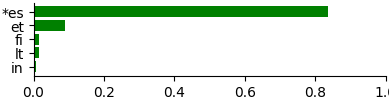
\includegraphics[width=0.45\textwidth]{img/infer/bar-lang-placeholder}
%\end{figure}

%Japanese (\begin{CJK}{UTF8}{min}クウェート\end{CJK})
%The translation of Kuwait in Chinese
%\begin{quote}
%\end{quote}
%
%Chinese (\begin{CJK}{UTF8}{min}科威特\end{CJK})
%Russian (\foreignlanguage{russian}{Кувейт})
%Greek (\foreignlanguage{greek}{κουβέιτ})

\end{description}

%%%%%%%%%%%%%%%%%%%%%%%%%%%%%%%%%%%%%%%%%%%%%%%%%%%%%%%%%%%%%%%%%%%%%%%%%%%%%%%%
\section{Our Model}
\label{sec:model}

\begin{figure*}
    \centering
    %\fbox{\parbox{\textwidth}{\vspace{2in}}}
    \resizebox{\textwidth}{!}{\definecolor{darkblue}{RGB}{0,0,127}
\begin{tikzpicture}
    [ node distance=5mm
    %, li/.style={anchor=west}
    %, l1/.style={ text width=4cm}
    %, tc/.style={anchor=north, text width=4cm}
    %, tc2/.style={li, minimum height=5mm}
    , box/.style=
        { draw=black
        , inner sep=2mm
        , rounded corners=1mm
        , minimum width=3cm
        , minimum height=1.3cm
        , fill=white
        }
    , output/.style={box} %, fill=lightblue}
    %, us/.style  ={->,line width=2pt,draw=green}
    %, them/.style={->,line width=1pt,draw=red,dotted}
    , every text node part/.style={align=center}
    ]
    \pgfdeclarelayer{background}
    \pgfsetlayers{background,main}
    \definecolor{lightblue}{rgb}{0.9,0.9,1.0}
    \definecolor{border}{rgb}{0.2,0.2,0.5}
    \newcommand{\headerA}[1]{\textbf{#1}}
    \newcommand{\headerB}[1]{\textsc{#1}}

    \node (unicodecnn) [box, draw=blue, opacity=0.5, fill=lightblue, minimum width=11cm, minimum height=5cm] at (7.5cm,-0.5cm) {};

    \node at (3.5cm,1.5cm) {\textcolor{darkblue}{UnicodeCNN}};

    \node (clcnn) [box, draw=blue, opacity=0.5, fill=lightblue, minimum width=7cm, minimum height=2.5cm] at (9.25cm,0.25cm) {};

    %\node (clcnn) [box, draw=blue, opacity=0.5, fill=lightblue, fit=(clcnn_label) (conv) (mix)] at (9.25cm,0.25cm) {};
    \node (clcnn_label) at (7.25cm,1cm) {\textcolor{darkblue}{CLCNN \citep{zhang2015character}}};

    \node (input) [box] at (0,0) {Input Text};
    \node (embed) [box, right=1cm of input.east] {Character\\Encoder};
    \node (conv) [box, right=of embed.east] {Convolutional\\Layers};

    \node (conv2) [right=1.5mm of conv.east, minimum height=1.3cm] {};

    \node (lang) [box, below=7mm of conv2.south] {Language\\Estimator};
    %\node (lang_f1) [box, below=of conv.south] {fully connected};
    %\node (lang_f2) [box, below=of lang_f1.south] {fully connected};
    %\node (lang) [output,below=of lang_f2.south] {language cross entropy};

    \node (mix) [box, right=of conv.east] {Feature Mixing};
    %\node (pos_f1) [box, right=of conv.east] {fully connected};
    %\node (pos_f2) [box, right=of pos_f1.east] {fully connected};
    \node (output) [right=23mm of mix.east] {};
    \node (country) [output, above =of output.east] {Country\\Cross Entropy};
    \node (fvm) [output, below =of output.east] {Mixture of\\von Mises-Fisher};

    \draw[->] (input) -- (embed);
    \draw[->] (embed) -- (conv);
    \draw[->] (conv) -- (mix);
    \draw[->] (mix) -- (country);
    \draw[->] (mix) -- (fvm);
    \draw[->] (conv.225) to[out=270,in=180] (lang);
    \draw[->] (lang) to[out=0,in=270] (mix.315);

    %\draw[->] (conv) -- (pos_f1);
    %\draw[->] (pos_f1) -- (pos_f2);
    %\draw[->] (pos_f2) -- (country);
    %\draw[->] (pos_f2) -- (fvm);
    %\draw[->] (conv) -- (lang_f1);
    %\draw[->] (lang_f1) -- (lang_f2);
    %\draw[->] (lang_f2) -- (lang);
    %\draw[->] (lang) to [out=0,in=270] (pos_f1);

\end{tikzpicture}

}
    \textbf{
    \caption{
        The UnicodeCNN adds a novel character embedding and language estimator to the \defn{character level convolutional neural network} (CLCNN) \citep{zhang2015character}.
        For the task of geolocation, we add two outputs to predict the country using the standard cross entropy loss and the GPS coordinates using a novel mixture of Fisher-von Mises distributions.
    %Structure of our UnicodeCNN model.  
    %Blue layers require supervision. 
    %We emphasize that the UnicodeCNN component is application agnostic,
    %and only the rightmost output layers are used for our geotagging application.
    %Other output layers can be used for other applications through transfer learning.
    %\fixme{beautify.}
    \label{fig:model}
    }
    }
\end{figure*}

The structure of our model is shown in Figure \ref{fig:model}.
The model is divided into two stages.
The first stage is the UnicodeCNN which extracts features from the input Unicode string.
The second stage is a mixture of Fisher-von Mises distributions which is used to predict the GPS locations of the tweet.
We emphasize that while the second stage is application specific,
the UnicodeCNN stage can be used on any application.
By using transfer learning \citep{wang2015transfer,howard2018fine},
the features generated by the UnicodeCNN can be reused for other applications.
%feature generation, feature mixing, and output.
%The model's output is then compared against the location data in the tweet to measure its efficacy.

%%%%%%%%%%%%%%%%%%%%%%%%%%%%%%%%%%%%%%%%
\subsection{The UnicodeCNN}

%The first step of our model is to convert the text of a tweet into a $d\times\ell$ matrix using a novel character hashing strategy.
The UnicodeCNN is divided into four steps.
First, the characters are encoded into a matrix;
Second, this matrix is the input to a series of convolutional layers;
these convolutional layers feed a language predictor module;
and the language predictor and convolutional layers together generate the final features.

Previous work using Unicode embeddings \citep{gillick2015multilingual,plank2016multilingual} learned directly on the UTF-8 encoding of Unicode characters.
This biases the models towards Latin languages (since their characters have simpler UTF-8 encodings)
and does not take advantage of the considerable amount of information baked into each Unicode code point.

\begin{description}
\item[Characer Encoding.]
Our encoding method has three important properties:
\begin{enumerate*}
    \item 
    Our encoding supports all Unicode code points%
    \footnote{
        A \defn{code point} is the basic unit of Unicode.
        Each ready-made character, diacritic mark, and combining instruction is represented by a different code point.
        %We very briefly describe relevant aspects of the Unicode standard,
        %but refer the reader to the official documentation \citep{Unicode} for further details.
    }.
    This is in contrast to previous work using character-level CNNs that only support English characters \citep{zhang2015character,conneau2017very}. 
    Supporting all Unicode code points is the fundamental improvement that lets our model use any language as input.
    \item 
    Our encoding is necessarily lossy because the Unicode standard can encode more than one million possible code points,
    whereas previous encodings could be lossless because they supported only the small English alphabet.
    Our experimental results show that a lossless encoding is not necessary.
    The later stages of the model are able to disambiguate encoding collisions from context.
    \item
    Our encoding associates similar encodings to similar characters from different scripts.
    %For example, the Cyrillic character П has a similar representation to the Latin P because they correspond to similar sounds.
    This helps ensure that our model is robust to both misspellings and transliteration between writing systems.
    %\item
    %Some complex code points have longer encodings than simple code points.
    %For example, the Japanese character
\end{enumerate*}

We now describe the encoding procedure in detail.
The first step is to normalize the string's representation using Unicode's NFKC normalization strategy.
This normalization is needed because many strings have multiple equivalent encodings in Unicode.
For example, consider the Vietnamese character \str{\foreignlanguage{vietnam}{Ớ}}.
This character can be encoded using the \str{U+1EDA} code point directly,
the code points \str{U+00D3} \str{U+031B}
(which corresponds to the accented \str{Ó} and a modifying mark),
the code points \str{U+004F} \str{U+031B} \str{U+0301}
(which corresponds to the Latin \str{O} and two modifying diacritic marks),
or many other combinations.
Normalizing the text ensures that all of these code point combinations get converted into a single canonical form.
Different normalization strategies consider different code point combinations equivalent,
and we choose the NFKC strategy because it combines code points most aggressively.

Next, we process each normalized code point individually.
%Most code points are assigned a $d$-bit encoding,
%but certain complex code points are assigned a $2d$ or $3d$ bit encoding.
Each code point is first transliterated into the Latin script.
Most code points are transliterated into a single character
(e.g.\ \str{\foreignlanguage{vietnam}{Ớ}} is transliterated into \str{O}),
but certain code points are transliterated into multiple characters
(e.g.\ the Chinese character \begin{CJK}{UTF8}{min}東\end{CJK} gets transliterated into \str{dong}).

\begin{description}[font=\normalfont\itshape]
\item[Bits 1-7:]
A one-hot encoding of the code point's \defn{Unicode category}.
Each code point is assigned one of seven possible categories:
letter,
mark,
number,
punctuation,
symbol,
separator,
or other.

\item[Bit 8:]
Set to one if the code point is either an upper case or title case character,
and zero otherwise.

\item[Bits 9-13:]
A one-hot encoding of the \defn{Unicode directionality}.
Each code point can have one of five possible Unicode directionalities:
strongly left-to-right (e.g.\ Latin letters),
strongly right-to-left (e.g.\ Arabic or Hebrew letters),
weak (e.g.\ numbers),
neutral (e.g.\ paragraph separators),
and explicit formatting commands.

\item[Bits 14-29:]
These bits encode any diacritic marks on the character as follows.
The character is decomposed into a ready-made character and marks using the NFD normalization scheme.
For example, the \str{U+1EDA} code point (\str{\foreignlanguage{vietnam}{Ớ}}) is decomposed into the Latin \str{O} and the two marks \str{U+031B} and \str{U+0301}.
Each mark is assigned a number between 0 and 15 by first multiplying the code point's value by a large prime, 
then taking the remainder mod 16.
Then, bit $14+r$ is set to 1 for each mark.
This part of the encoding is lossy because many diacritic marks will be assigned the same encoding.

\item[Bits 30-57:]
    Bit 30 is set to 1 if the character is \str{\#},
    and bit 31 is set to 1 if the character is \str{@}.
    These characters have special importance in Twitter (indicating hashtags and mentions),
    and so are important enough to have their own bit.
    Bit 32 is set to 1 if the romanization of the code point is \str{a},
    bit 33 if the romanization is \str{b},
    and so on until bit 57 if the romanization is \str{z}.

\item[Bit 58:]
Set to 1 if the character is actually from the Latin alphabet.

\item[Bit 59:]
Set to 1 if the character is the first character in a transliteration string.

\item[Bit 60-$d$:]
    If the character is from the Latin alphabet, all these bits are set to 0.
    Otherwise, the code point is multiplied by a large prime and the remainder $r$ with respect to $d-60$ is taken.
    Bit $60+r$ is then set to 1.
\end{description}

\ignore{
A weakness of our transliteration scheme is that certain characters should be transliterated in different ways depending on context,
but we ignore context.
The simplest type of context is the language of the text.
Different languages pronounce different characters differently,
and hence the character should be transliterated differently.
For example, the Chinese character \begin{CJK}{UTF8}{min}東\end{CJK} (which means East) should be transliterated as \str{dong} if the text is written in Mandarin Chinese 
(using the Pinyin transliteration scheme),
as \str{dung} if the text is written in Cantonese Chinese 
(using the Jyutping transliteration scheme),
or as \str{tang} if the text is written in Hokkien Chinese 
(using the POJ transliteration scheme).
Sometimes, however, just knowing the language is not enough information to effectively transliterate.
For example, the Japense Kanji writing system uses Chinese characters,
but the pronunciation of those characters changes from word to word.
The two most common pronunciation schemes are the Onyomi and Kunyomi,
which transliterate \begin{CJK}{UTF8}{min}東\end{CJK} as \str{tou} and \str{higashi} respectively.
Certain proper nouns, however, use the rarer Nanori pronunciation, which for  \begin{CJK}{UTF8}{min}東\end{CJK} can be any of \str{ai}, \str{agari}, \str{ko}, \str{saki}, \str{shino}, \str{hajime}, \str{higa}, or \str{moto} depending on the name.
These difficulties are most pronounced in East Asian languages,
and a more sophisticated transliteration scheme could therefore possibly improve performance for these languages.
}

%%%%%%%%%%%%%%%%%%%%%%%%%%%%%%%%%%%%%%%%

\item[Character Convolutions.]
    The character encoding matrix described above is passed as the input to a series of six temporal convolutional layers.
    Temporal convolution is a standard deep learning tool,
    and a full description is beyond the scope of this paper.
    Here, we briefly describe the intuition behind these convolutional layers and state the parameters that we use.
    We refer the reader to the \emph{Deep Learning Book} \citep{Goodfellow-et-al-2016} and the original paper on character level convolutional neural networks (CLCNNs) \citep{zhang2015character} for mathematical details.

    Intuitively, a convolutional layer generates a new ``higher level'' set of features from the input ``low level'' features.
    These higher level features are formed by convolving a suitable \defn{filter} with the input matrix, 
    then optionally performing \defn{max-pooling}.
    There are two important parameters: the number of channels and the width.
    The number of channels determines the number of filters that are applied in parallel,
    each creating its own set of output features.
    Increasing the number of channels increases the model's ability to detect important linguistic features,
    but it also increases the computational complexity of the model and the model's ability to overfit the data.
    Our Large and Small models use the same number of channels as the original CLCNN \citep{zhang2015character},
    and our Huge model uses twice as many channels.
    We are able to use such a large model because our massive dataset prevents overfitting,
    and we train our model in parallel using 8 GPUs (see Section \ref{sec:experiments}).
    The width of a convolutional or max-pooling layer determines the number of input features that get combined into a single output feature.
    Increasing the width of a convolutional layer increases model capacity 
    (again at the expense of computation time and overfitting),
    whereas increasing the width of a max-pooling layer decreases model capacity.

    The following table describes the parameters of the 6 convolutional layers.
    Each model size uses a different number of channels, but the same widths.

    \begin{table}[H]
    \begin{tabular}{c|ccc|cc}
        & \multicolumn{3}{|c|}{Channels} & \multicolumn{2}{c}{Width} \\
        Layer & Huge & Large & Small & Kernel & Max-Pool \\
        \hline
        1 & 2048 & 1024 & 256 & 7 & 3 \\
        2 & 2048 & 1024 & 256 & 7 & 3 \\
        3 & 2048 & 1024 & 256 & 3 & N/A \\
        4 & 2048 & 1024 & 256 & 3 & N/A \\
        5 & 2048 & 1024 & 256 & 3 & N/A \\
        6 & 2048 & 1024 & 256 & 3 & 3 \\
    \end{tabular}
    \end{table}

    \noindent
    An important property of the output features is the number of input characters that had a role in generating the feature.
    The formula for calculating this is $1 + \sum(\text{width of each layer} - 1)$.
    In our case, this comes out to be 27.

%We use a \defn{convolutional neural network (CNN)} to generate character-level features.
%Specifically, our model is a variant of the CLCNN \citep{zhang2015character}.
%The input encoding matrix is passed to 

Alternative character-level models use deeper CNNs with resnet connections \citep{conneau2017very}, recurrent neural networks (RNNs) \citep{chung2016character}, 
or complex combinations of CNNs and RNNs \citep{kim2016character,jozefowicz2016exploring}.
Each of these techniques requires considerable processing resources, however, 
so we did not have the resources to exhaustively compare these techniques to each other on this task.
We chose to base our model off of the CLCNN model because it had the best performance on a small held-out subset of tweets.
All of these techniques were originally designed to work on relatively small mono-lingual corpuses.
The largest dataset used in the papers above is \fixme{},
whereas our dataset is \fixme{}.

Deep learning techniques have also been applied to Twitter data.
%Character-level models have previously been applied to twitter NLP tasks \citep[e.g.][]{dhingra2016tweet2vec,severyn2015unitn},
%but never to the geolocation problem.
For example, 
\citet{severyn2015unitn} use a word level CNN for sentiment classification on tweets,
and \citet{dhingra2016tweet2vec} use a character level GRU network to predict hashtags.
Ours is the first application of deep learning techniques to the geolocation problem,
uses the largest dataset,
and the first multilingual dataset.
%Their dataset contains only 2 million tweets, whereas our dataset contains \fixme{}.

%\item[Word-level features.]
%All previous work on twitter geolocation has essentially relied on hand-crafted world-level features.
%\citet{han2012geolocation} study a method of determining location indicative words using an information gain strategy.

\item[Language.]
There are two ways to incorporate language of a tweet into our model.
The first is to use the Twitter API's language field directly 1-hot encoded.
This is a simple technique, but has three drawbacks:
(i) the Twitter API supports many fewer languages than are actually used on Twitter;
(ii) the Twitter API occasionally makes mistakes on which language the tweet was sent in;
(iii) Twitter uses an undisclosed algorithm to determine the language,
and this algorithm is likely to leak user-level meta-information.

An alternative is to try to learn the language directly.

\fixme{
We use \str{langid.py} \citep{lui2012langid} to count the number of known languages in our dataset.
\str{langid.py} supports 97 languages, and all 97 were identified in our dataset.
We additionally identified tweets written in three languages not supported by \str{langid.py}: 
Burmese, Maldivian, and Sindhi.
In total, our dataset contains at least 100 languages, 
and likely many more that we have not identified.
}

%The \str{lang} field of a tweet is determined automatically by the twitter software using a combination of unpublished tweet and user level features.
%\citet{blodgett2016demographic} show that existing language prediction tools such as \str{langid.py} \citep{lui2012langid} perform poorly relative to the \str{lang} field of the json object.
%This effect is exacerbated when the tweets exhibit dialectical differences from the formal version of their language.
%\end{description}

%\item[Language.]
The Twitter API associates with each tweet one of 65 possible officially supported languages.
The most popular language is English with $405\times10^6$ tweets,
and the least popular language is Uighur with only 157 tweets.
Many other languages are also present in our dataset, however.
$74\times10^6$ tweets are classified as being from an undefined language.
This can happen when the tweet contains too little text to determine the language,
or when the language is not one of Twitter's officially recognized 65 languages.
%For example, we have identified that the set of tweets with undefined language contains tweets in Czechoslovakian.
For example, Croatian is not an officially supported language,
and so tweets written in Croatian get classified as having an undefined language.
Furthermore, many unofficial languages get miscategorized into similar languages that are officially recognized.
For example, 
tweets written in Catalan get classified as Spanish,
and tweets written in Malay get classified as Indonesian.
Because the dataset is so large,
we make no effort to exhaustively identify all the languages it contains.
Previous efforts to categorize the number of languages found on Twitter fouond more than 100 different languages \citep{hong2011language}.
\fixme{Section XXX of the supplement shows examples of our language-agnostic model discovering these unofficial languages by itself and exploiting them for geolocating.}

\item[Feature Mixing.]
Our model uses two fully connected layers with 2048 hidden units each and relu activation functions.
%To reduce overfitting, each of these layers is trained using dropout and a 50\% keep probability \citep{}.

\begin{table}[H]
\begin{tabular}{c|ccc}
    & \multicolumn{3}{c}{Output Units} \\
    Layer & Huge & Large & Small \\
    \hline
    7 & 4096 & 2048 & 1024 \\
    8 & 4096 & 2048 & 1024 \\
    %9 &  &  &  \\
\end{tabular}
\end{table}
\end{description}

%%%%%%%%%%%%%%%%%%%%

\subsection{Model Output}

Our model has two outputs that indicate the location of the tweet at two levels of granularity.

\begin{description}

    \item[Country.]
        Determining which country the tweet was sent from is a standard classification problem with 248 classes.
        We therefore use the standard softmax crossentropy loss.

    \item[GPS Coordinates.]
        As discussed in Section \ref{sec:problems:output},
        determining the exact GPS coordinates of a tweet is not a classification problem,
        and previous work either chose not to predict GPS coordinates 
        or used an incorrect model to predict GPS coordinates that did not consider the non-Euclidean nature of the earth's surface.
        In this section, 
        we introduce a novel output layer for our network called the \defn{Mixture of Fischer-von Mises distributions} (MFvM layer).
        The MFvM layer outputs a probability distribution over the earth's surface for each tweet,
        and a point estimate of the tweet's location can be computed using the maximum likelihood.

        The MFvM layer is inspired by the field of \defn{directional statistics},
        which studies distributions on the surface of hyperspheres.
        The \defn{Fischer-von Mises} (FvM) distribution is one of the standard distributions studied in directional statistics and can be considered the spherical analogue of the Gaussian distribution \citep[e.g.][]{mardia2009directional}.
        Thus, mixtures of FvM distributions can be seen as the spherical analogue of the commonly used mixture of Gaussian distributions.
        While the mixture of FvM distributions has previously been used in deep learning for clustering \citep{gopal2014mises} and facial recognition \citep{hasnat2017mises},
        we believe we are the first to apply it to predicting GPS coordinates.

        The optimization of the MFvM output layer is closely related to optimization of deep learning models with a mixture of Gaussians layer \citep{variani2015gaussian},
        except the Gaussian density is replaced by the FvM density.
        The density of the FvM distribution is given by
        \begin{equation}
            \text{FvM}(\x;\kappa,\mu) = \frac{\kappa}{\sinh \kappa} \exp(\kappa\trans\mu\x),
        \end{equation}
        where $\kappa\in\mathbb R$ is called the \defn{concentration parameter},
        $\mu\in\mathbb{S}^2$ is called the \defn{mean direction},
        and $\x$ is any point in $\mathbb{S}^2$,
        and $\mathbb{S}^2 = \{ \x \in \mathbb R^3 : \ltwo{\x}=1 \}$ is the unit sphere.
        The overall loss is then
        \begin{equation}
            -\log\sum_{i=1}^q {\omega}_i \text{FvM}(\x;\kappa_i,\mu_i),
        \end{equation}
        where $q$ is the total number of FvM distributions and the $\omega_i$ are constrained to sum to 1.
        The $\omega_i$, $\kappa_i$, and $\mu_i$ parameters are all trainable.
        To speed up convergence, we initialize $\omega_i=1/q$ and 
        $\kappa_i=\exp(8)$.
        We initialized $\mu_i$ by setting it equal to the location on the sphere of the world's $i$th most populated city.

\end{description}

%%%%%%%%%%%%%%%%%%%%%%%%%%%%%%%%%%%%%%%%
\ignore{
\subsection{Prediction losses}

Our general framework has two types of outputs:
discrete outputs that estimate the \place and \country fields of the tweet,
and continuous outputs that estimate the \geo field.
%Whereas previous work requires a number of assumptions about the output fields,
%our work makes few assumptions.

\begin{description}
\item[Discrete outputs.]
The discrete outputs are conceptually the simplest,
and for this reason they are the most commonly used in previous work.
The idea is to treat a tweet's \place and \country fields as labels for the tweet,
then perform ordinary multi-label classification using the cross entropy loss.
Our work differs from previous work because no previous work has attempted to directly predict a tweet's \place field.
Because there are millions of distinct \place entries in twitter,
this task was considered too hard.
Instead, previous work constructed \pseudoplace labels that filter out uncommonly seen entries and merge them into other nearby locations.
This reduces the number of class labels from millions down to thousands,
making a much easier problem.

There is no standard method for constructing these \pseudoplace labels in the literature.
\citet{han2012geolocation} proposed a more sophisticated method.
Their method combines suburbs with nearby cities,
and identifies a total of 3709 cities to use as class labels.
Those tweets that do not originate from a city are either discarded or assigned to the closest city.
More complicated methods of discretizing the Earth's surface have also been developed for non-Twitter applications.
For example, Google developed a large scale system for geolocating images that uses specially designed partition of the earth's surface that they call S2 \citep{weyand2016planet}.

\item[Angular regression.]
We introduce novel methods for predicting the \geo field that take advantage of the non-euclidean nature of the earth's surface.
\citet{duong2016near} is the only previous work to attempt to estimate the \geo field of a tweet.
They use the ordinary least squares regression model with the standard $L2$ loss between GPS coordinates:
\begin{equation}
    \latd^2 + \lond^2
    .
\end{equation}
Unfortunately, the surface of the earth is highly non-euclidean, 
and the OLS model is known to work only in the euclidean setting \citep[e.g.][]{fisher1992regression}.
For example:
\begin{enumerate}
    \item
        There is a difficulty at the antimeridian (180 degrees west).
        The antimeridean approximately separates Russian from Alaska.
        The true distance between these locations is very short (about 100km),
        but the distance using the L2 norm is very large.
    \item
        Second, the standard $L2$ loss does not accurately capture the distance between GPS coordinates.
        For example, at a latitude of 80 degrees north, 1 degree of longitude is approximately equal to 20 km;
        but at the equator, 1 degree of longitude is approximately equal to 111 km.
\end{enumerate}

The so-called \emph{angular regression} fixes these problems \citep{fisher1992regression}.
\citet{fisher1992regression} was the first to propose a method for regression onto the surface of a sphere.

The \emph{great circle distance} is a better distance metric for gps coordinates because it is the distance of the shortest path between two points on the earth's surface.
The naive computation of the great circle distance is unfortunately numerically unstable and cannot be used directly.
Fortunately, \citet{vincenty1975direct} proposed a numerically stable method for computing the GCD which we use in our work.
Figure \ref{fig:vincenty} shows the formula.

\begin{figure*}
    \centering
    %\begin{align}
    $
    \displaystyle
        \delta\sigma 
        =
        \arctan\left(
            \frac
            {\sqrt{(\cos\lata\cdot\sin\lond)^2 + (\cos\lata\cdot\sin\latb-\sin\lata\cdot\cos\latb\cdot\cos\lond)^2}}
            {\sin\lata\cdot\sin\latb + \cos\lata\cdot\cos\latb\cdot\cos\lond}
        \right)
    $
    %\end{align}
    \caption{The Vincenty formula for numerically stable great circle distances.}
    \label{fig:vincenty}
\end{figure*}

\item[Mixture of FvM.]

\end{description}
}

%%%%%%%%%%%%%%%%%%%%%%%%%%%%%%%%%%%%%%%%%%%%%%%%%%%%%%%%%%%%%%%%%%%%%%%%%%%%%%%%

\section{Experiments}
\label{sec:experiments}

We now describe our dataset, 
training and evaluation method, 
baseline comparison models, 
and results.

\begin{description}
        %
%%%%%%%%%%%%%%%%%%%%%%%%%%%%%%%%%%%%%%%%

\item[Dataset.]
Our dataset contains all tweets with geolocation information sent between 26 October 2017 and 08 July 2018.
The dataset contains approximately 900 million tweets written by $3.0$ million users.
Unlike previous work, 
we perform no filtering to remove ``hard'' tweets from the dataset,
and as a result our dataset is orders of magnitude larger than previously used datasets.

%The WORLD dataset \citep{han2012geolocation} contains $1.4\times10^6$ users and $12\times10^6$ tweets.
The largest previously used dataset for geolocating tweets was previously the WORLD+ML dataset \citep{han2014text},
which contains only $23$ million tweets written by $2.1$ million users.
WORLD+ML includes tweets in all languages,
but removes hard-to-geolocate tweets that are not close to major cities.
Whereas the WORLD+ML dataset contained only 47\% non-English tweets,
our dataset contains 68\% non-English tweets.
Other datasets such as the WNUT \citep{han2016twitter}, WORLD \citep{han2012geolocation}, and NA \citep{roller2012supervised}
additionally remove non-English tweets and so are considerably smaller.

For each tweet in our dataset, we associate a country and GPS coordinates using the Twitter API.
The Twitter API defines a total of 247 unique country codes that a tweet can be sent from.
This number is larger than the number of sovereign states recognized by the United Nations (206)
because many non-countries (e.g.\ Puerto Rico and Hong Kong) are given country codes.
The process of assigning GPS coordinates is slightly more complicated.
User privacy settings allow Twitter to share the exact GPS coordinates of approximately 16\% of tweets in our dataset.
For the remaining tweets, privacy settings restrict the accuracy that the tweet's location can be shared to a higher level, typically the city.
In this case, we take the center of mass of the associated city as the true GPS location of the tweet.
There are approximately 3 million unique city-level locations reported by the Twitter API.
The WNUT \citep{han2016twitter}, WORLD \citep{han2012geolocation}, and WORLD+ML \citep{han2014text} datasets generated class labels using a complex procedure to:
(i) select approximately the 3000 most populated of these cities,
(ii) combine them with nearby cities into a single metropolitan area which serves as the class label,
and (iii) discard all tweets from cities not from these metropolitan areas.
Clearly, significant amounts of information are lost when creating class labels in this way.
Our method of using the GPS coordinates preserves as much information from the tweet as possible and creates a more challenging prediction problem.

%%%%%%%%%%%%%%%%%%%%%%%%%%%%%%%%%%%%%%%%

\begin{figure}
    %\resizebox{0.225\textwidth}{!}{% GNUPLOT: LaTeX picture with Postscript
\begingroup
  \makeatletter
  \providecommand\color[2][]{%
    \GenericError{(gnuplot) \space\space\space\@spaces}{%
      Package color not loaded in conjunction with
      terminal option `colourtext'%
    }{See the gnuplot documentation for explanation.%
    }{Either use 'blacktext' in gnuplot or load the package
      color.sty in LaTeX.}%
    \renewcommand\color[2][]{}%
  }%
  \providecommand\includegraphics[2][]{%
    \GenericError{(gnuplot) \space\space\space\@spaces}{%
      Package graphicx or graphics not loaded%
    }{See the gnuplot documentation for explanation.%
    }{The gnuplot epslatex terminal needs graphicx.sty or graphics.sty.}%
    \renewcommand\includegraphics[2][]{}%
  }%
  \providecommand\rotatebox[2]{#2}%
  \@ifundefined{ifGPcolor}{%
    \newif\ifGPcolor
    \GPcolorfalse
  }{}%
  \@ifundefined{ifGPblacktext}{%
    \newif\ifGPblacktext
    \GPblacktexttrue
  }{}%
  % define a \g@addto@macro without @ in the name:
  \let\gplgaddtomacro\g@addto@macro
  % define empty templates for all commands taking text:
  \gdef\gplbacktext{}%
  \gdef\gplfronttext{}%
  \makeatother
  \ifGPblacktext
    % no textcolor at all
    \def\colorrgb#1{}%
    \def\colorgray#1{}%
  \else
    % gray or color?
    \ifGPcolor
      \def\colorrgb#1{\color[rgb]{#1}}%
      \def\colorgray#1{\color[gray]{#1}}%
      \expandafter\def\csname LTw\endcsname{\color{white}}%
      \expandafter\def\csname LTb\endcsname{\color{black}}%
      \expandafter\def\csname LTa\endcsname{\color{black}}%
      \expandafter\def\csname LT0\endcsname{\color[rgb]{1,0,0}}%
      \expandafter\def\csname LT1\endcsname{\color[rgb]{0,1,0}}%
      \expandafter\def\csname LT2\endcsname{\color[rgb]{0,0,1}}%
      \expandafter\def\csname LT3\endcsname{\color[rgb]{1,0,1}}%
      \expandafter\def\csname LT4\endcsname{\color[rgb]{0,1,1}}%
      \expandafter\def\csname LT5\endcsname{\color[rgb]{1,1,0}}%
      \expandafter\def\csname LT6\endcsname{\color[rgb]{0,0,0}}%
      \expandafter\def\csname LT7\endcsname{\color[rgb]{1,0.3,0}}%
      \expandafter\def\csname LT8\endcsname{\color[rgb]{0.5,0.5,0.5}}%
    \else
      % gray
      \def\colorrgb#1{\color{black}}%
      \def\colorgray#1{\color[gray]{#1}}%
      \expandafter\def\csname LTw\endcsname{\color{white}}%
      \expandafter\def\csname LTb\endcsname{\color{black}}%
      \expandafter\def\csname LTa\endcsname{\color{black}}%
      \expandafter\def\csname LT0\endcsname{\color{black}}%
      \expandafter\def\csname LT1\endcsname{\color{black}}%
      \expandafter\def\csname LT2\endcsname{\color{black}}%
      \expandafter\def\csname LT3\endcsname{\color{black}}%
      \expandafter\def\csname LT4\endcsname{\color{black}}%
      \expandafter\def\csname LT5\endcsname{\color{black}}%
      \expandafter\def\csname LT6\endcsname{\color{black}}%
      \expandafter\def\csname LT7\endcsname{\color{black}}%
      \expandafter\def\csname LT8\endcsname{\color{black}}%
    \fi
  \fi
  \setlength{\unitlength}{0.0500bp}%
  \begin{picture}(5040.00,3240.00)%
    \gplgaddtomacro\gplbacktext{%
      \csname LTb\endcsname%
      \put(264,660){\makebox(0,0)[r]{\strut{}\scriptsize 0.0}}%
      \put(264,1239){\makebox(0,0)[r]{\strut{}\scriptsize 0.1}}%
      \put(264,1818){\makebox(0,0)[r]{\strut{}\scriptsize 0.2}}%
      \put(264,2396){\makebox(0,0)[r]{\strut{}\scriptsize 0.3}}%
      \put(264,2975){\makebox(0,0)[r]{\strut{}\scriptsize 0.4}}%
      \put(580,528){\rotatebox{-45}{\makebox(0,0)[l]{\strut{}\scriptsize~USA}}}%
      \put(949,528){\rotatebox{-45}{\makebox(0,0)[l]{\strut{}\scriptsize~Brazil}}}%
      \put(1318,528){\rotatebox{-45}{\makebox(0,0)[l]{\strut{}\scriptsize~Japan}}}%
      \put(1687,528){\rotatebox{-45}{\makebox(0,0)[l]{\strut{}\scriptsize~UK}}}%
      \put(2056,528){\rotatebox{-45}{\makebox(0,0)[l]{\strut{}\scriptsize~TR}}}%
      \put(2425,528){\rotatebox{-45}{\makebox(0,0)[l]{\strut{}\scriptsize~Philippines}}}%
      \put(2794,528){\rotatebox{-45}{\makebox(0,0)[l]{\strut{}\scriptsize~Argentina}}}%
      \put(3163,528){\rotatebox{-45}{\makebox(0,0)[l]{\strut{}\scriptsize~Saudi~Arabia}}}%
      \put(3532,528){\rotatebox{-45}{\makebox(0,0)[l]{\strut{}\scriptsize~Spain}}}%
      \put(3901,528){\rotatebox{-45}{\makebox(0,0)[l]{\strut{}\scriptsize~Mexico}}}%
      \put(4270,528){\rotatebox{-45}{\makebox(0,0)[l]{\strut{}\scriptsize~other}}}%
      \put(-242,1817){\rotatebox{-270}{\makebox(0,0){\strut{}\scriptsize fraction of tweets}}}%
      \put(2425,2865){\makebox(0,0){\strut{}Most Active Countries}}%
    }%
    \gplgaddtomacro\gplfronttext{%
    }%
    \gplbacktext
    \put(0,0){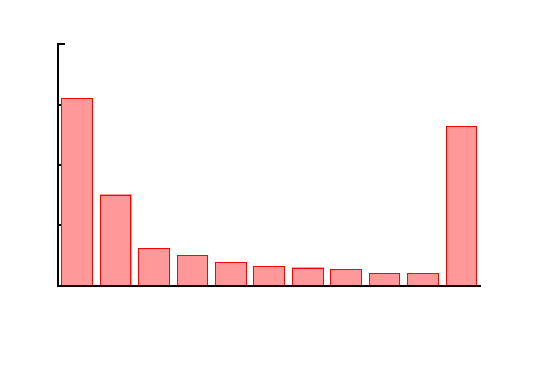
\includegraphics{img/country}}%
    \gplfronttext
  \end{picture}%
\endgroup
}
    %\centering

    \hspace{0.5in}
    \resizebox{0.45\textwidth}{!}{% GNUPLOT: LaTeX picture with Postscript
\begingroup
  \makeatletter
  \providecommand\color[2][]{%
    \GenericError{(gnuplot) \space\space\space\@spaces}{%
      Package color not loaded in conjunction with
      terminal option `colourtext'%
    }{See the gnuplot documentation for explanation.%
    }{Either use 'blacktext' in gnuplot or load the package
      color.sty in LaTeX.}%
    \renewcommand\color[2][]{}%
  }%
  \providecommand\includegraphics[2][]{%
    \GenericError{(gnuplot) \space\space\space\@spaces}{%
      Package graphicx or graphics not loaded%
    }{See the gnuplot documentation for explanation.%
    }{The gnuplot epslatex terminal needs graphicx.sty or graphics.sty.}%
    \renewcommand\includegraphics[2][]{}%
  }%
  \providecommand\rotatebox[2]{#2}%
  \@ifundefined{ifGPcolor}{%
    \newif\ifGPcolor
    \GPcolorfalse
  }{}%
  \@ifundefined{ifGPblacktext}{%
    \newif\ifGPblacktext
    \GPblacktexttrue
  }{}%
  % define a \g@addto@macro without @ in the name:
  \let\gplgaddtomacro\g@addto@macro
  % define empty templates for all commands taking text:
  \gdef\gplbacktext{}%
  \gdef\gplfronttext{}%
  \makeatother
  \ifGPblacktext
    % no textcolor at all
    \def\colorrgb#1{}%
    \def\colorgray#1{}%
  \else
    % gray or color?
    \ifGPcolor
      \def\colorrgb#1{\color[rgb]{#1}}%
      \def\colorgray#1{\color[gray]{#1}}%
      \expandafter\def\csname LTw\endcsname{\color{white}}%
      \expandafter\def\csname LTb\endcsname{\color{black}}%
      \expandafter\def\csname LTa\endcsname{\color{black}}%
      \expandafter\def\csname LT0\endcsname{\color[rgb]{1,0,0}}%
      \expandafter\def\csname LT1\endcsname{\color[rgb]{0,1,0}}%
      \expandafter\def\csname LT2\endcsname{\color[rgb]{0,0,1}}%
      \expandafter\def\csname LT3\endcsname{\color[rgb]{1,0,1}}%
      \expandafter\def\csname LT4\endcsname{\color[rgb]{0,1,1}}%
      \expandafter\def\csname LT5\endcsname{\color[rgb]{1,1,0}}%
      \expandafter\def\csname LT6\endcsname{\color[rgb]{0,0,0}}%
      \expandafter\def\csname LT7\endcsname{\color[rgb]{1,0.3,0}}%
      \expandafter\def\csname LT8\endcsname{\color[rgb]{0.5,0.5,0.5}}%
    \else
      % gray
      \def\colorrgb#1{\color{black}}%
      \def\colorgray#1{\color[gray]{#1}}%
      \expandafter\def\csname LTw\endcsname{\color{white}}%
      \expandafter\def\csname LTb\endcsname{\color{black}}%
      \expandafter\def\csname LTa\endcsname{\color{black}}%
      \expandafter\def\csname LT0\endcsname{\color{black}}%
      \expandafter\def\csname LT1\endcsname{\color{black}}%
      \expandafter\def\csname LT2\endcsname{\color{black}}%
      \expandafter\def\csname LT3\endcsname{\color{black}}%
      \expandafter\def\csname LT4\endcsname{\color{black}}%
      \expandafter\def\csname LT5\endcsname{\color{black}}%
      \expandafter\def\csname LT6\endcsname{\color{black}}%
      \expandafter\def\csname LT7\endcsname{\color{black}}%
      \expandafter\def\csname LT8\endcsname{\color{black}}%
    \fi
  \fi
  \setlength{\unitlength}{0.0500bp}%
  \begin{picture}(5040.00,3240.00)%
    \gplgaddtomacro\gplbacktext{%
      \csname LTb\endcsname%
      \put(264,660){\makebox(0,0)[r]{\strut{}\scriptsize 0.0}}%
      \put(264,1123){\makebox(0,0)[r]{\strut{}\scriptsize 0.1}}%
      \put(264,1586){\makebox(0,0)[r]{\strut{}\scriptsize 0.2}}%
      \put(264,2049){\makebox(0,0)[r]{\strut{}\scriptsize 0.3}}%
      \put(264,2512){\makebox(0,0)[r]{\strut{}\scriptsize 0.4}}%
      \put(264,2975){\makebox(0,0)[r]{\strut{}\scriptsize 0.5}}%
      \put(580,528){\rotatebox{-45}{\makebox(0,0)[l]{\strut{}\scriptsize~English}}}%
      \put(949,528){\rotatebox{-45}{\makebox(0,0)[l]{\strut{}\scriptsize~Portuguese}}}%
      \put(1318,528){\rotatebox{-45}{\makebox(0,0)[l]{\strut{}\scriptsize~Spanish}}}%
      \put(1687,528){\rotatebox{-45}{\makebox(0,0)[l]{\strut{}\scriptsize~Unknown$^*$}}}%
      \put(2056,528){\rotatebox{-45}{\makebox(0,0)[l]{\strut{}\scriptsize~Japanese}}}%
      \put(2425,528){\rotatebox{-45}{\makebox(0,0)[l]{\strut{}\scriptsize~Arabic}}}%
      \put(2794,528){\rotatebox{-45}{\makebox(0,0)[l]{\strut{}\scriptsize~Turkish}}}%
      \put(3163,528){\rotatebox{-45}{\makebox(0,0)[l]{\strut{}\scriptsize~Indonesian}}}%
      \put(3532,528){\rotatebox{-45}{\makebox(0,0)[l]{\strut{}\scriptsize~Tagalog}}}%
      \put(3901,528){\rotatebox{-45}{\makebox(0,0)[l]{\strut{}\scriptsize~French}}}%
      \put(4270,528){\rotatebox{-45}{\makebox(0,0)[l]{\strut{}\scriptsize~other}}}%
      \put(-242,1817){\rotatebox{-270}{\makebox(0,0){\strut{}\scriptsize fraction of tweets}}}%
      \put(2425,2865){\makebox(0,0){\strut{}Most Active Languages}}%
    }%
    \gplgaddtomacro\gplfronttext{%
    }%
    \gplbacktext
    \put(0,0){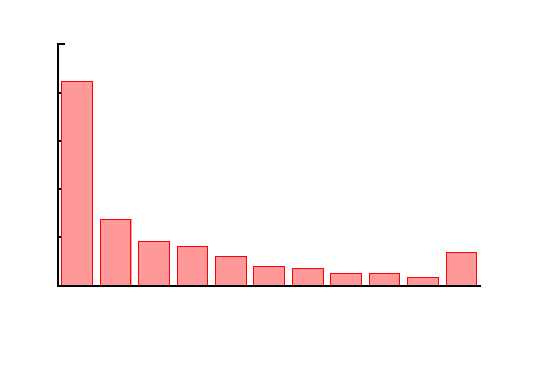
\includegraphics{img/lang}}%
    \gplfronttext
  \end{picture}%
\endgroup
}
    \hspace{-0.5in}

    \textbf{
    \caption{
        Language distribution of tweets in our dataset.
        Most tweets are not written in English,
        but prior work focuses on this special case.
        (*) Twitter classifies approximately 8\% of tweets in our dataset as having an unknown language.
        This may be because the tweet is written in a language that Twitter does not officially support,
        or because the tweet has too little text.
        %Most tweets are neither located in the United States nor in English,
        %but prior work focuses on these two special cases.
    }
    }
    \label{fig:country/lang}
\end{figure}


%%%%%%%%%%%%%%%%%%%%%%%%%%%%%%%%%%%%%%%%

\begin{table*}

\begin{tabular}{l|c|cccccccc}
& average &\multicolumn{8}{c}{accuracy} \\
model & distance (km) & @country & @10 & @50 & @100 & @500 & @1000 & @2000 & @3000 \\
\hline
\hline
early-cnn & 3710.13 & 0.69 & 0.00 & 0.01 & 0.02 & 0.23 & 0.39 & 0.53 & 0.59 \\
 early-lang & 7230.26 & 0.63 & 0.00 & 0.01 & 0.03 & 0.12 & 0.16 & 0.19 & 0.20 \\
 early-langtime-256x256 & 8227.62 & 0.31 & 0.00 & 0.00 & 0.00 & 0.00 & 0.00 & 0.00 & 0.00 \\
 early-time & 7686.67 & 0.25 & 0.00 & 0.00 & 0.00 & 0.02 & 0.05 & 0.11 & 0.16 \\
 \end{tabular}
%\begin{tabular}{l|c|ccccccc}
& average &\multicolumn{8}{c}{accuracy} \\
model & distance (km) & @50km & @100km & @500km & @1000km & @2000km & @3000km & @country \\
\hline
\str{lang} & 2302.225 & 0.533 & 0.573 & 0.714 & 0.787 & 0.827 & 0.840 & 0.640 \\
\str{lang+time} & 2210.765 & 0.531 & 0.571 & 0.714 & 0.789 & 0.831 & 0.847 & 0.646 \\
\str{lang+time+bow} & 1738.139 & 0.563 & 0.615 & 0.763 & 0.832 & 0.867 & 0.884 & 0.731 \\
UnicodeCNN (Small) & 1519.381 & 0.562 & 0.611 & 0.767 & 0.842 & 0.885 & 0.903 & 0.746 \\
UnicodeCNN (Large) & --&--&--&--&--&--&--&--&-- \\
UnicodeCNN (Huge) & 1379.444 & 0.254 & 0.345 & 0.618 & 0.747 & 0.820 & 0.852 & 0.767 \\
 \end{tabular}

\textbf{
\caption{
    The UnicodeCNN features give the best results across all measures,
    with the larger UnicodeCNN's giving better results than the smaller ones.
    Recall that smaller values indicate better performance for average distance and larger values are better for accuracy.
    \label{table:results}
}
}
\end{table*}

%%%%%%%%%%%%%%%%%%%%%%%%%%%%%%%%%%%%%%%%

\item[Baseline Models.]

We compare our UnicodeCNN with three baseline models.
All three models predict the country and gps coordinates a tweet was sent from,
the only difference is the way the features are generated.

The first model, \str{lang} uses only the language of the tweet 1-hot encoded as an input feature.
This is the simplest reasonable model for the multilingual geolocation problem.
This model is able to capture the fact that different countries use different languages,
but is unable learn patterns about how different regions use different dialects of the same language or discuss different topics.

The second model, \str{lang+time} uses the language features above and time features.
Many languages (e.g.\ Spanish) are used in different countries,
and so the language alone cannot discriminate between these countries.
%Combining language and time
%The time that the tweet was sent may be able to disambiguate these countries,
%however.
We generate features from the day of week and time of day that the tweet was sent,
and the \str{lang+time} model uses these time features in addition to the language features.

%Neither the \str{lang} nor \str{lang+time} models directly inspect the text of the tweet.
The final model, \str{lang+time+bow} adds bag-of-words features to the model generated from the text.
Bag-of-words features are a classic method for analyzing English-language text corpora,
and our model follows best practices.
In particular, we use feature hashing \citep{weinberger2009feature} with L1 regularization to automatically select the best features.
Bag-of-words features are the most popular features used in content-based tweet geolocation,
and they have been used in all the following papers:
\citep{cheng2010you,kinsella2011m,li2012towards,han2013stacking,mahmud2014home,compton2014geotagging,zhang2014geocoding,rahimi2015twitter,dredze2016geolocation,rahimi2017neural}.

\fixme{
The results from these papers are not directly comparable to the results in our paper for two reasons.
First, we consider a harder geolocation problem than previous papers.
We perform no filtering of the dataset to remove difficult tweets,
and we attempt to determine exact GPS positions rather than just nearby cities.
Second, many of the previous papers augment the bag-of-words features using special preprocessing of the text that is only applicable to the English language.
For example, \citep{} use an English-language gazetteer to additionally create features for locations that appear within the text,
and \citep{} use the English-only lexical analyzer XXX \citep{}.
}

%\begin{figure*}
%\noindent% GNUPLOT: LaTeX picture with Postscript
\begingroup
  \makeatletter
  \providecommand\color[2][]{%
    \GenericError{(gnuplot) \space\space\space\@spaces}{%
      Package color not loaded in conjunction with
      terminal option `colourtext'%
    }{See the gnuplot documentation for explanation.%
    }{Either use 'blacktext' in gnuplot or load the package
      color.sty in LaTeX.}%
    \renewcommand\color[2][]{}%
  }%
  \providecommand\includegraphics[2][]{%
    \GenericError{(gnuplot) \space\space\space\@spaces}{%
      Package graphicx or graphics not loaded%
    }{See the gnuplot documentation for explanation.%
    }{The gnuplot epslatex terminal needs graphicx.sty or graphics.sty.}%
    \renewcommand\includegraphics[2][]{}%
  }%
  \providecommand\rotatebox[2]{#2}%
  \@ifundefined{ifGPcolor}{%
    \newif\ifGPcolor
    \GPcolorfalse
  }{}%
  \@ifundefined{ifGPblacktext}{%
    \newif\ifGPblacktext
    \GPblacktexttrue
  }{}%
  % define a \g@addto@macro without @ in the name:
  \let\gplgaddtomacro\g@addto@macro
  % define empty templates for all commands taking text:
  \gdef\gplbacktext{}%
  \gdef\gplfronttext{}%
  \makeatother
  \ifGPblacktext
    % no textcolor at all
    \def\colorrgb#1{}%
    \def\colorgray#1{}%
  \else
    % gray or color?
    \ifGPcolor
      \def\colorrgb#1{\color[rgb]{#1}}%
      \def\colorgray#1{\color[gray]{#1}}%
      \expandafter\def\csname LTw\endcsname{\color{white}}%
      \expandafter\def\csname LTb\endcsname{\color{black}}%
      \expandafter\def\csname LTa\endcsname{\color{black}}%
      \expandafter\def\csname LT0\endcsname{\color[rgb]{1,0,0}}%
      \expandafter\def\csname LT1\endcsname{\color[rgb]{0,1,0}}%
      \expandafter\def\csname LT2\endcsname{\color[rgb]{0,0,1}}%
      \expandafter\def\csname LT3\endcsname{\color[rgb]{1,0,1}}%
      \expandafter\def\csname LT4\endcsname{\color[rgb]{0,1,1}}%
      \expandafter\def\csname LT5\endcsname{\color[rgb]{1,1,0}}%
      \expandafter\def\csname LT6\endcsname{\color[rgb]{0,0,0}}%
      \expandafter\def\csname LT7\endcsname{\color[rgb]{1,0.3,0}}%
      \expandafter\def\csname LT8\endcsname{\color[rgb]{0.5,0.5,0.5}}%
    \else
      % gray
      \def\colorrgb#1{\color{black}}%
      \def\colorgray#1{\color[gray]{#1}}%
      \expandafter\def\csname LTw\endcsname{\color{white}}%
      \expandafter\def\csname LTb\endcsname{\color{black}}%
      \expandafter\def\csname LTa\endcsname{\color{black}}%
      \expandafter\def\csname LT0\endcsname{\color{black}}%
      \expandafter\def\csname LT1\endcsname{\color{black}}%
      \expandafter\def\csname LT2\endcsname{\color{black}}%
      \expandafter\def\csname LT3\endcsname{\color{black}}%
      \expandafter\def\csname LT4\endcsname{\color{black}}%
      \expandafter\def\csname LT5\endcsname{\color{black}}%
      \expandafter\def\csname LT6\endcsname{\color{black}}%
      \expandafter\def\csname LT7\endcsname{\color{black}}%
      \expandafter\def\csname LT8\endcsname{\color{black}}%
    \fi
  \fi
  \setlength{\unitlength}{0.0500bp}%
  \begin{picture}(10080.00,2520.00)%
    \gplgaddtomacro\gplbacktext{%
      \csname LTb\endcsname%
      \put(176,1281){\rotatebox{-270}{\makebox(0,0){\strut{}\scriptsize fraction of tweets}}}%
      \put(3779,154){\makebox(0,0){\strut{}\scriptsize time of day (UTC)}}%
      \put(3779,2189){\makebox(0,0){\strut{}Countries that Tweet in English}}%
    }%
    \gplgaddtomacro\gplfronttext{%
      \csname LTb\endcsname%
      \put(396,374){\makebox(0,0){\strut{}\scriptsize 0:00}}%
      \put(1242,374){\makebox(0,0){\strut{}\scriptsize 3:00}}%
      \put(2088,374){\makebox(0,0){\strut{}\scriptsize 6:00}}%
      \put(2934,374){\makebox(0,0){\strut{}\scriptsize 9:00}}%
      \put(3780,374){\makebox(0,0){\strut{}\scriptsize 12:00}}%
      \put(4625,374){\makebox(0,0){\strut{}\scriptsize 15:00}}%
      \put(5471,374){\makebox(0,0){\strut{}\scriptsize 18:00}}%
      \put(6317,374){\makebox(0,0){\strut{}\scriptsize 21:00}}%
      \put(7163,374){\makebox(0,0){\strut{}\scriptsize 24:00}}%
    }%
    \gplgaddtomacro\gplbacktext{%
      \csname LTb\endcsname%
      \put(9083,154){\makebox(0,0){\strut{}~~}}%
      \put(9083,2189){\makebox(0,0){\strut{} }}%
    }%
    \gplgaddtomacro\gplfronttext{%
      \csname LTb\endcsname%
      \put(8352,751){\makebox(0,0)[r]{\strut{}\scriptsize~USA}}%
      \put(8352,868){\makebox(0,0)[r]{\strut{}\scriptsize~UK}}%
      \put(8352,985){\makebox(0,0)[r]{\strut{}\scriptsize~Philippines}}%
      \put(8352,1102){\makebox(0,0)[r]{\strut{}\scriptsize~Canada}}%
      \put(8352,1219){\makebox(0,0)[r]{\strut{}\scriptsize~India}}%
      \put(8352,1337){\makebox(0,0)[r]{\strut{}\scriptsize~South~Africa}}%
      \put(8352,1454){\makebox(0,0)[r]{\strut{}\scriptsize~Australia}}%
      \put(8352,1571){\makebox(0,0)[r]{\strut{}\scriptsize~Malasia}}%
      \put(8352,1688){\makebox(0,0)[r]{\strut{}\scriptsize~Nigeria}}%
      \put(8352,1805){\makebox(0,0)[r]{\strut{}\scriptsize~Brazil}}%
      \put(8352,1922){\makebox(0,0)[r]{\strut{}\scriptsize~other}}%
    }%
    \gplbacktext
    \put(0,0){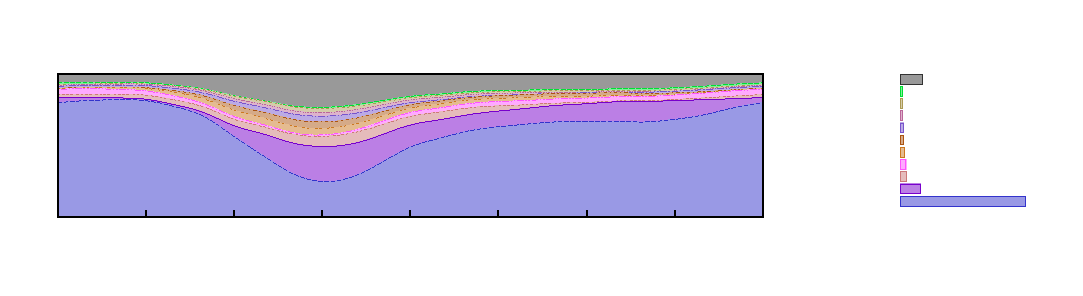
\includegraphics{img/hr-en}}%
    \gplfronttext
  \end{picture}%
\endgroup

%\noindent% GNUPLOT: LaTeX picture with Postscript
\begingroup
  \makeatletter
  \providecommand\color[2][]{%
    \GenericError{(gnuplot) \space\space\space\@spaces}{%
      Package color not loaded in conjunction with
      terminal option `colourtext'%
    }{See the gnuplot documentation for explanation.%
    }{Either use 'blacktext' in gnuplot or load the package
      color.sty in LaTeX.}%
    \renewcommand\color[2][]{}%
  }%
  \providecommand\includegraphics[2][]{%
    \GenericError{(gnuplot) \space\space\space\@spaces}{%
      Package graphicx or graphics not loaded%
    }{See the gnuplot documentation for explanation.%
    }{The gnuplot epslatex terminal needs graphicx.sty or graphics.sty.}%
    \renewcommand\includegraphics[2][]{}%
  }%
  \providecommand\rotatebox[2]{#2}%
  \@ifundefined{ifGPcolor}{%
    \newif\ifGPcolor
    \GPcolorfalse
  }{}%
  \@ifundefined{ifGPblacktext}{%
    \newif\ifGPblacktext
    \GPblacktexttrue
  }{}%
  % define a \g@addto@macro without @ in the name:
  \let\gplgaddtomacro\g@addto@macro
  % define empty templates for all commands taking text:
  \gdef\gplbacktext{}%
  \gdef\gplfronttext{}%
  \makeatother
  \ifGPblacktext
    % no textcolor at all
    \def\colorrgb#1{}%
    \def\colorgray#1{}%
  \else
    % gray or color?
    \ifGPcolor
      \def\colorrgb#1{\color[rgb]{#1}}%
      \def\colorgray#1{\color[gray]{#1}}%
      \expandafter\def\csname LTw\endcsname{\color{white}}%
      \expandafter\def\csname LTb\endcsname{\color{black}}%
      \expandafter\def\csname LTa\endcsname{\color{black}}%
      \expandafter\def\csname LT0\endcsname{\color[rgb]{1,0,0}}%
      \expandafter\def\csname LT1\endcsname{\color[rgb]{0,1,0}}%
      \expandafter\def\csname LT2\endcsname{\color[rgb]{0,0,1}}%
      \expandafter\def\csname LT3\endcsname{\color[rgb]{1,0,1}}%
      \expandafter\def\csname LT4\endcsname{\color[rgb]{0,1,1}}%
      \expandafter\def\csname LT5\endcsname{\color[rgb]{1,1,0}}%
      \expandafter\def\csname LT6\endcsname{\color[rgb]{0,0,0}}%
      \expandafter\def\csname LT7\endcsname{\color[rgb]{1,0.3,0}}%
      \expandafter\def\csname LT8\endcsname{\color[rgb]{0.5,0.5,0.5}}%
    \else
      % gray
      \def\colorrgb#1{\color{black}}%
      \def\colorgray#1{\color[gray]{#1}}%
      \expandafter\def\csname LTw\endcsname{\color{white}}%
      \expandafter\def\csname LTb\endcsname{\color{black}}%
      \expandafter\def\csname LTa\endcsname{\color{black}}%
      \expandafter\def\csname LT0\endcsname{\color{black}}%
      \expandafter\def\csname LT1\endcsname{\color{black}}%
      \expandafter\def\csname LT2\endcsname{\color{black}}%
      \expandafter\def\csname LT3\endcsname{\color{black}}%
      \expandafter\def\csname LT4\endcsname{\color{black}}%
      \expandafter\def\csname LT5\endcsname{\color{black}}%
      \expandafter\def\csname LT6\endcsname{\color{black}}%
      \expandafter\def\csname LT7\endcsname{\color{black}}%
      \expandafter\def\csname LT8\endcsname{\color{black}}%
    \fi
  \fi
  \setlength{\unitlength}{0.0500bp}%
  \begin{picture}(10080.00,2520.00)%
    \gplgaddtomacro\gplbacktext{%
      \csname LTb\endcsname%
      \put(176,1281){\rotatebox{-270}{\makebox(0,0){\strut{}\scriptsize fraction of tweets}}}%
      \put(3779,154){\makebox(0,0){\strut{}\scriptsize time of day (UTC)}}%
      \put(3779,2189){\makebox(0,0){\strut{}Countries that Tweet in Spanish}}%
    }%
    \gplgaddtomacro\gplfronttext{%
      \csname LTb\endcsname%
      \put(396,374){\makebox(0,0){\strut{}\scriptsize 0:00}}%
      \put(1242,374){\makebox(0,0){\strut{}\scriptsize 3:00}}%
      \put(2088,374){\makebox(0,0){\strut{}\scriptsize 6:00}}%
      \put(2934,374){\makebox(0,0){\strut{}\scriptsize 9:00}}%
      \put(3780,374){\makebox(0,0){\strut{}\scriptsize 12:00}}%
      \put(4625,374){\makebox(0,0){\strut{}\scriptsize 15:00}}%
      \put(5471,374){\makebox(0,0){\strut{}\scriptsize 18:00}}%
      \put(6317,374){\makebox(0,0){\strut{}\scriptsize 21:00}}%
      \put(7163,374){\makebox(0,0){\strut{}\scriptsize 24:00}}%
    }%
    \gplgaddtomacro\gplbacktext{%
      \csname LTb\endcsname%
      \put(9083,154){\makebox(0,0){\strut{}~~}}%
      \put(9083,2189){\makebox(0,0){\strut{} }}%
    }%
    \gplgaddtomacro\gplfronttext{%
      \csname LTb\endcsname%
      \put(8352,751){\makebox(0,0)[r]{\strut{}\scriptsize~Argentina}}%
      \put(8352,868){\makebox(0,0)[r]{\strut{}\scriptsize~Spain}}%
      \put(8352,985){\makebox(0,0)[r]{\strut{}\scriptsize~Mexico}}%
      \put(8352,1102){\makebox(0,0)[r]{\strut{}\scriptsize~Colombia}}%
      \put(8352,1219){\makebox(0,0)[r]{\strut{}\scriptsize~Chile}}%
      \put(8352,1337){\makebox(0,0)[r]{\strut{}\scriptsize~USA}}%
      \put(8352,1454){\makebox(0,0)[r]{\strut{}\scriptsize~Venezuela}}%
      \put(8352,1571){\makebox(0,0)[r]{\strut{}\scriptsize~Brazil}}%
      \put(8352,1688){\makebox(0,0)[r]{\strut{}\scriptsize~Uruguay}}%
      \put(8352,1805){\makebox(0,0)[r]{\strut{}\scriptsize~PE}}%
      \put(8352,1922){\makebox(0,0)[r]{\strut{}\scriptsize~other}}%
    }%
    \gplbacktext
    \put(0,0){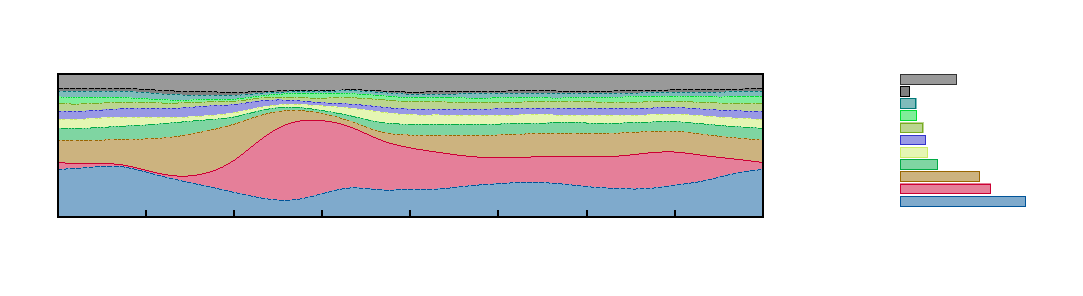
\includegraphics{img/hr-es}}%
    \gplfronttext
  \end{picture}%
\endgroup

%\textbf{
%\caption{
    %Different countries tweet in different languages and at different times of the day.
    %For example, tweets sent in English are almost always sent from the United States,
    %except around 9AM UTC (2AM PST).
    %Tweets sent in Spanish are likely to be sent from either Argentina (from 2200UTC-0400UTC), Mexico (0500-0600UTC), or Spain (0600-2200UTC).
    %\fixme{Remove whitespace.}
%}
%}
%\label{fig:time-lang}
%\end{figure*}

\fixme{
Metadata associated with each tweet has also been used to generate features,
and this metadata can significantly improve geolocation performance.
For example, 
\citep{hecht2011tweets,schulz2013multi,han2014text}.
And the social graph \citep{}.
We do not compare against these models, however, because we are only interested in content-based geolocation.
}

%%%%%%%%%%%%%%%%%%%%%%%%%%%%%%%%%%%%%%%%

%%\item[User Metadata.]
%The JSON object also contains significant information about the user who sent the tweet.
%This metadata can be used to greatly increase the accuracy of geolocation 
%\citep{hecht2011tweets,schulz2013multi,han2014text}.
%We do not consider this metadata in our prediction problem;
%however, because it obscures the ability to predict locations from the text.
%
%For example, the metadata contains a user specified timezone field.
%The timezone provides a surprisingly large amount of detail about a tweet's location.
%At the bare minimum, 
%the timezone determines the tweets longitude with high accuracy,
%and so the problem of geolocating with timezone information reduces to the problem of determining the tweet's latitude.
%Some timezones (like Hawaiian Standard Time) determine both longitude and latitude with high accuracy,
%and so the tweet's text doesn't even need to be examined to perform geolocation.
%Furthermore, weets in Hawaiian Standard Time fit within a small 100km radius, which means the text doesn't even have to be examined.
%For timezones like Hawaiian Standard Time,
%this is an exceedingly easy problem.
%Knowledge of the timezone transforms the problem into only predicting latitude.
%For example, essentially all tweets in Hawaiian Standard Time fit within a small 100km radius, which means the text doesn't even have to be examined.
%Time zone information can also encode country location directly.
%For example, Korea and Japan have essentially the same longitude, 
%and so use the same offset from UTC for their time.
%But they have different timezones (denoted Korea Standard Time and Japan Standard Time).
%Knowledge of the timezone in these cases is sufficient to completely determine the country of origin.

%%%%%%%%%%%%%%%%%%%%%%%%%%%%%%%%%%%%%%%%

\item[Training and Evaluation Procedure.]
We train and evaluate our models in an online fashion using the Adam optimizer \citep{kingma2014adam}.
That is, we perform a single pass over the dataset.
For each tweet, we first compute the loss of the model on that tweet;
then we update the model's parameters.
The total loss is then the sum of the individual tweet losses.
We choose this evaluation method because it is a natural model for tweet geolocation where new data can easily be obtained and it is efficient computationally.

We use three types of losses to evaluate the models' performance.
The \defn{distance} measures the average distance between a tweet's true location and the point estimate given by the MFvM output.
The \defn{accuracy @50km} is the percent of tweets whose distance error is less than 50km.
The {accuracy @100km, @500km, 1000km, 2000km, and 3000km} measures are similar.
Finally, the \defn{accuracy @country} measures the percent of tweets whose country of origin was correctly predicted.
Numeric results are shown in Table \ref{table:results}.

To train the UnicodeCNN models,
we use a single machine with 16 CPUs, 64 GB of RAM, and 6 NVidia Titan x80 GPUs. 
We train using the Adam optimizer \citep{kingma2014adam} with a learning rate of $5\times10^{-4}$ and a batch size of 600.
We train in using data parallelism, so that each GPU processes 100 tweets per batch, 
and then the gradients are averaged together.
%The learning rate was set by training only on a small held-out subset of tweets,
The batch size of 100 tweets/GPU is the largest batchsize we could fit on a GPU with the huge model.
We observed about a 5-fold speed up using all 6 GPUs,
and in total, training the large model took about four weeks with this setup.
Training the huge model seems to take about \fixme{} time.
We let it train for two weeks but then ran out of time.
We expect the huge model's performance would continue to slightly improve given more training time.

All baseline models were trained using Adam \citep{kingma2014adam} and random hyperparameter search \citep{bergstra2012random}.
Random hyperparameter search is a state-of-the-art hyperparameter tuning method that requires no manual intervention and works well when there is more than one hyperparameter to tune.
For each model, we randomly selected a learning rate, L2 regularization strength, and (for the \str{lang+time+bow} model only) L1 regularization strength in the range $10^{-6}$ to $10^0$ distributed uniformly over the logarithm.
We trained 20 versions of each model and report only the best model.

\end{description}

%%%%%%%%%%%%%%%%%%%%%%%%%%%%%%%%%%%%%%%%%%%%%%%%%%%%%%%%%%%%%%%%%%%%%%%%%%%%%%%%
\ignore{
\newpage
\section{Visualization}

A major disadvantage of CNNs is that they lack interpretability compared to simpler models.
To alleviate this problem, many techniques have been proposed to visualize CNNs in the context of image classification \citep{zeiler2014visualizing,seifert2017visualizations}.
We adapt these methods to provide the first visualization method of CNNs applicable to the text domain.
This visualization technique helps us understand the dialectical patterns that \uniloc~CNN discovers in the text.

The method is simple and inspired by the occlusion method proposed by \citet{zeiler2014visualizing} for visualizing image CNNs.
Given an input text with $n$ characters,
we generate $n-1$ new texts by removing the $i$th character from the original text.
}

%%%%%%%%%%%%%%%%%%%%%%%%%%%%%%%%%%%%%%%%%%%%%%%%%%%%%%%%%%%%%%%%%%%%%%%%%%%%%%%%

\newpage
\appendix
\ignore{
\section{Languages and Day of Week}
\noindent% GNUPLOT: LaTeX picture with Postscript
\begingroup
  \makeatletter
  \providecommand\color[2][]{%
    \GenericError{(gnuplot) \space\space\space\@spaces}{%
      Package color not loaded in conjunction with
      terminal option `colourtext'%
    }{See the gnuplot documentation for explanation.%
    }{Either use 'blacktext' in gnuplot or load the package
      color.sty in LaTeX.}%
    \renewcommand\color[2][]{}%
  }%
  \providecommand\includegraphics[2][]{%
    \GenericError{(gnuplot) \space\space\space\@spaces}{%
      Package graphicx or graphics not loaded%
    }{See the gnuplot documentation for explanation.%
    }{The gnuplot epslatex terminal needs graphicx.sty or graphics.sty.}%
    \renewcommand\includegraphics[2][]{}%
  }%
  \providecommand\rotatebox[2]{#2}%
  \@ifundefined{ifGPcolor}{%
    \newif\ifGPcolor
    \GPcolorfalse
  }{}%
  \@ifundefined{ifGPblacktext}{%
    \newif\ifGPblacktext
    \GPblacktexttrue
  }{}%
  % define a \g@addto@macro without @ in the name:
  \let\gplgaddtomacro\g@addto@macro
  % define empty templates for all commands taking text:
  \gdef\gplbacktext{}%
  \gdef\gplfronttext{}%
  \makeatother
  \ifGPblacktext
    % no textcolor at all
    \def\colorrgb#1{}%
    \def\colorgray#1{}%
  \else
    % gray or color?
    \ifGPcolor
      \def\colorrgb#1{\color[rgb]{#1}}%
      \def\colorgray#1{\color[gray]{#1}}%
      \expandafter\def\csname LTw\endcsname{\color{white}}%
      \expandafter\def\csname LTb\endcsname{\color{black}}%
      \expandafter\def\csname LTa\endcsname{\color{black}}%
      \expandafter\def\csname LT0\endcsname{\color[rgb]{1,0,0}}%
      \expandafter\def\csname LT1\endcsname{\color[rgb]{0,1,0}}%
      \expandafter\def\csname LT2\endcsname{\color[rgb]{0,0,1}}%
      \expandafter\def\csname LT3\endcsname{\color[rgb]{1,0,1}}%
      \expandafter\def\csname LT4\endcsname{\color[rgb]{0,1,1}}%
      \expandafter\def\csname LT5\endcsname{\color[rgb]{1,1,0}}%
      \expandafter\def\csname LT6\endcsname{\color[rgb]{0,0,0}}%
      \expandafter\def\csname LT7\endcsname{\color[rgb]{1,0.3,0}}%
      \expandafter\def\csname LT8\endcsname{\color[rgb]{0.5,0.5,0.5}}%
    \else
      % gray
      \def\colorrgb#1{\color{black}}%
      \def\colorgray#1{\color[gray]{#1}}%
      \expandafter\def\csname LTw\endcsname{\color{white}}%
      \expandafter\def\csname LTb\endcsname{\color{black}}%
      \expandafter\def\csname LTa\endcsname{\color{black}}%
      \expandafter\def\csname LT0\endcsname{\color{black}}%
      \expandafter\def\csname LT1\endcsname{\color{black}}%
      \expandafter\def\csname LT2\endcsname{\color{black}}%
      \expandafter\def\csname LT3\endcsname{\color{black}}%
      \expandafter\def\csname LT4\endcsname{\color{black}}%
      \expandafter\def\csname LT5\endcsname{\color{black}}%
      \expandafter\def\csname LT6\endcsname{\color{black}}%
      \expandafter\def\csname LT7\endcsname{\color{black}}%
      \expandafter\def\csname LT8\endcsname{\color{black}}%
    \fi
  \fi
  \setlength{\unitlength}{0.0500bp}%
  \begin{picture}(10080.00,2520.00)%
    \gplgaddtomacro\gplbacktext{%
      \csname LTb\endcsname%
      \put(176,1281){\rotatebox{-270}{\makebox(0,0){\strut{}\scriptsize fraction of tweets}}}%
      \put(3779,154){\makebox(0,0){\strut{}\scriptsize day of week(UTC)}}%
      \put(3779,2189){\makebox(0,0){\strut{}Countries that Tweet in English}}%
    }%
    \gplgaddtomacro\gplfronttext{%
      \csname LTb\endcsname%
      \put(396,374){\makebox(0,0){\strut{}\scriptsize 0}}%
      \put(1363,374){\makebox(0,0){\strut{}\scriptsize 1}}%
      \put(2329,374){\makebox(0,0){\strut{}\scriptsize 2}}%
      \put(3296,374){\makebox(0,0){\strut{}\scriptsize 3}}%
      \put(4263,374){\makebox(0,0){\strut{}\scriptsize 4}}%
      \put(5230,374){\makebox(0,0){\strut{}\scriptsize 5}}%
      \put(6196,374){\makebox(0,0){\strut{}\scriptsize 6}}%
      \put(7163,374){\makebox(0,0){\strut{}\scriptsize 7}}%
    }%
    \gplgaddtomacro\gplbacktext{%
      \csname LTb\endcsname%
      \put(9083,154){\makebox(0,0){\strut{}~~}}%
      \put(9083,2189){\makebox(0,0){\strut{} }}%
    }%
    \gplgaddtomacro\gplfronttext{%
      \csname LTb\endcsname%
      \put(8352,751){\makebox(0,0)[r]{\strut{}\scriptsize~USA}}%
      \put(8352,868){\makebox(0,0)[r]{\strut{}\scriptsize~UK}}%
      \put(8352,985){\makebox(0,0)[r]{\strut{}\scriptsize~Philippines}}%
      \put(8352,1102){\makebox(0,0)[r]{\strut{}\scriptsize~Canada}}%
      \put(8352,1219){\makebox(0,0)[r]{\strut{}\scriptsize~India}}%
      \put(8352,1337){\makebox(0,0)[r]{\strut{}\scriptsize~South~Africa}}%
      \put(8352,1454){\makebox(0,0)[r]{\strut{}\scriptsize~Australia}}%
      \put(8352,1571){\makebox(0,0)[r]{\strut{}\scriptsize~Malasia}}%
      \put(8352,1688){\makebox(0,0)[r]{\strut{}\scriptsize~Nigeria}}%
      \put(8352,1805){\makebox(0,0)[r]{\strut{}\scriptsize~Brazil}}%
      \put(8352,1922){\makebox(0,0)[r]{\strut{}\scriptsize~other}}%
    }%
    \gplbacktext
    \put(0,0){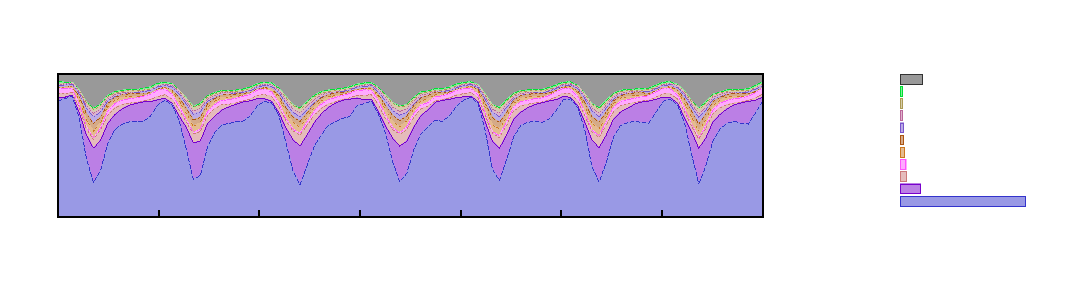
\includegraphics{img/day-en}}%
    \gplfronttext
  \end{picture}%
\endgroup


\noindent% GNUPLOT: LaTeX picture with Postscript
\begingroup
  \makeatletter
  \providecommand\color[2][]{%
    \GenericError{(gnuplot) \space\space\space\@spaces}{%
      Package color not loaded in conjunction with
      terminal option `colourtext'%
    }{See the gnuplot documentation for explanation.%
    }{Either use 'blacktext' in gnuplot or load the package
      color.sty in LaTeX.}%
    \renewcommand\color[2][]{}%
  }%
  \providecommand\includegraphics[2][]{%
    \GenericError{(gnuplot) \space\space\space\@spaces}{%
      Package graphicx or graphics not loaded%
    }{See the gnuplot documentation for explanation.%
    }{The gnuplot epslatex terminal needs graphicx.sty or graphics.sty.}%
    \renewcommand\includegraphics[2][]{}%
  }%
  \providecommand\rotatebox[2]{#2}%
  \@ifundefined{ifGPcolor}{%
    \newif\ifGPcolor
    \GPcolorfalse
  }{}%
  \@ifundefined{ifGPblacktext}{%
    \newif\ifGPblacktext
    \GPblacktexttrue
  }{}%
  % define a \g@addto@macro without @ in the name:
  \let\gplgaddtomacro\g@addto@macro
  % define empty templates for all commands taking text:
  \gdef\gplbacktext{}%
  \gdef\gplfronttext{}%
  \makeatother
  \ifGPblacktext
    % no textcolor at all
    \def\colorrgb#1{}%
    \def\colorgray#1{}%
  \else
    % gray or color?
    \ifGPcolor
      \def\colorrgb#1{\color[rgb]{#1}}%
      \def\colorgray#1{\color[gray]{#1}}%
      \expandafter\def\csname LTw\endcsname{\color{white}}%
      \expandafter\def\csname LTb\endcsname{\color{black}}%
      \expandafter\def\csname LTa\endcsname{\color{black}}%
      \expandafter\def\csname LT0\endcsname{\color[rgb]{1,0,0}}%
      \expandafter\def\csname LT1\endcsname{\color[rgb]{0,1,0}}%
      \expandafter\def\csname LT2\endcsname{\color[rgb]{0,0,1}}%
      \expandafter\def\csname LT3\endcsname{\color[rgb]{1,0,1}}%
      \expandafter\def\csname LT4\endcsname{\color[rgb]{0,1,1}}%
      \expandafter\def\csname LT5\endcsname{\color[rgb]{1,1,0}}%
      \expandafter\def\csname LT6\endcsname{\color[rgb]{0,0,0}}%
      \expandafter\def\csname LT7\endcsname{\color[rgb]{1,0.3,0}}%
      \expandafter\def\csname LT8\endcsname{\color[rgb]{0.5,0.5,0.5}}%
    \else
      % gray
      \def\colorrgb#1{\color{black}}%
      \def\colorgray#1{\color[gray]{#1}}%
      \expandafter\def\csname LTw\endcsname{\color{white}}%
      \expandafter\def\csname LTb\endcsname{\color{black}}%
      \expandafter\def\csname LTa\endcsname{\color{black}}%
      \expandafter\def\csname LT0\endcsname{\color{black}}%
      \expandafter\def\csname LT1\endcsname{\color{black}}%
      \expandafter\def\csname LT2\endcsname{\color{black}}%
      \expandafter\def\csname LT3\endcsname{\color{black}}%
      \expandafter\def\csname LT4\endcsname{\color{black}}%
      \expandafter\def\csname LT5\endcsname{\color{black}}%
      \expandafter\def\csname LT6\endcsname{\color{black}}%
      \expandafter\def\csname LT7\endcsname{\color{black}}%
      \expandafter\def\csname LT8\endcsname{\color{black}}%
    \fi
  \fi
  \setlength{\unitlength}{0.0500bp}%
  \begin{picture}(10080.00,2520.00)%
    \gplgaddtomacro\gplbacktext{%
      \csname LTb\endcsname%
      \put(176,1281){\rotatebox{-270}{\makebox(0,0){\strut{}\scriptsize fraction of tweets}}}%
      \put(3779,154){\makebox(0,0){\strut{}\scriptsize day of week(UTC)}}%
      \put(3779,2189){\makebox(0,0){\strut{}Countries that Tweet in Arabic}}%
    }%
    \gplgaddtomacro\gplfronttext{%
      \csname LTb\endcsname%
      \put(396,374){\makebox(0,0){\strut{}\scriptsize 0}}%
      \put(1363,374){\makebox(0,0){\strut{}\scriptsize 1}}%
      \put(2329,374){\makebox(0,0){\strut{}\scriptsize 2}}%
      \put(3296,374){\makebox(0,0){\strut{}\scriptsize 3}}%
      \put(4263,374){\makebox(0,0){\strut{}\scriptsize 4}}%
      \put(5230,374){\makebox(0,0){\strut{}\scriptsize 5}}%
      \put(6196,374){\makebox(0,0){\strut{}\scriptsize 6}}%
      \put(7163,374){\makebox(0,0){\strut{}\scriptsize 7}}%
    }%
    \gplgaddtomacro\gplbacktext{%
      \csname LTb\endcsname%
      \put(9083,154){\makebox(0,0){\strut{}~~}}%
      \put(9083,2189){\makebox(0,0){\strut{} }}%
    }%
    \gplgaddtomacro\gplfronttext{%
      \csname LTb\endcsname%
      \put(8352,751){\makebox(0,0)[r]{\strut{}\scriptsize~Saudi~Arabia}}%
      \put(8352,868){\makebox(0,0)[r]{\strut{}\scriptsize~Egypt}}%
      \put(8352,985){\makebox(0,0)[r]{\strut{}\scriptsize~Kuwait}}%
      \put(8352,1102){\makebox(0,0)[r]{\strut{}\scriptsize~Arab~Emirates}}%
      \put(8352,1219){\makebox(0,0)[r]{\strut{}\scriptsize~Qatar}}%
      \put(8352,1337){\makebox(0,0)[r]{\strut{}\scriptsize~Bahrain}}%
      \put(8352,1454){\makebox(0,0)[r]{\strut{}\scriptsize~Oman}}%
      \put(8352,1571){\makebox(0,0)[r]{\strut{}\scriptsize~USA}}%
      \put(8352,1688){\makebox(0,0)[r]{\strut{}\scriptsize~Iraq}}%
      \put(8352,1805){\makebox(0,0)[r]{\strut{}\scriptsize~UK}}%
      \put(8352,1922){\makebox(0,0)[r]{\strut{}\scriptsize~other}}%
    }%
    \gplbacktext
    \put(0,0){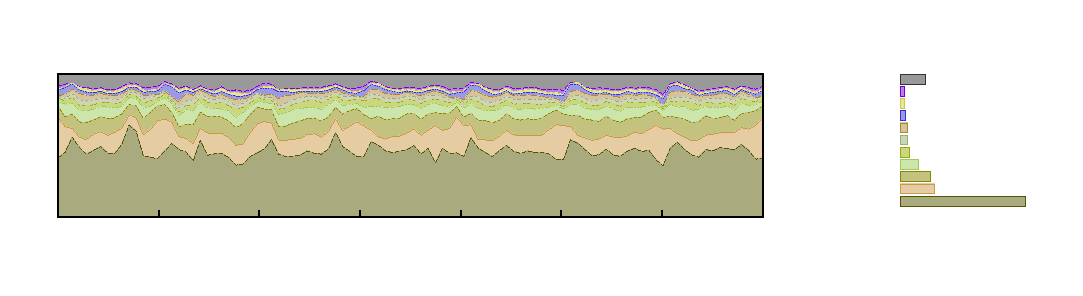
\includegraphics{img/day-ar}}%
    \gplfronttext
  \end{picture}%
\endgroup


\noindent% GNUPLOT: LaTeX picture with Postscript
\begingroup
  \makeatletter
  \providecommand\color[2][]{%
    \GenericError{(gnuplot) \space\space\space\@spaces}{%
      Package color not loaded in conjunction with
      terminal option `colourtext'%
    }{See the gnuplot documentation for explanation.%
    }{Either use 'blacktext' in gnuplot or load the package
      color.sty in LaTeX.}%
    \renewcommand\color[2][]{}%
  }%
  \providecommand\includegraphics[2][]{%
    \GenericError{(gnuplot) \space\space\space\@spaces}{%
      Package graphicx or graphics not loaded%
    }{See the gnuplot documentation for explanation.%
    }{The gnuplot epslatex terminal needs graphicx.sty or graphics.sty.}%
    \renewcommand\includegraphics[2][]{}%
  }%
  \providecommand\rotatebox[2]{#2}%
  \@ifundefined{ifGPcolor}{%
    \newif\ifGPcolor
    \GPcolorfalse
  }{}%
  \@ifundefined{ifGPblacktext}{%
    \newif\ifGPblacktext
    \GPblacktexttrue
  }{}%
  % define a \g@addto@macro without @ in the name:
  \let\gplgaddtomacro\g@addto@macro
  % define empty templates for all commands taking text:
  \gdef\gplbacktext{}%
  \gdef\gplfronttext{}%
  \makeatother
  \ifGPblacktext
    % no textcolor at all
    \def\colorrgb#1{}%
    \def\colorgray#1{}%
  \else
    % gray or color?
    \ifGPcolor
      \def\colorrgb#1{\color[rgb]{#1}}%
      \def\colorgray#1{\color[gray]{#1}}%
      \expandafter\def\csname LTw\endcsname{\color{white}}%
      \expandafter\def\csname LTb\endcsname{\color{black}}%
      \expandafter\def\csname LTa\endcsname{\color{black}}%
      \expandafter\def\csname LT0\endcsname{\color[rgb]{1,0,0}}%
      \expandafter\def\csname LT1\endcsname{\color[rgb]{0,1,0}}%
      \expandafter\def\csname LT2\endcsname{\color[rgb]{0,0,1}}%
      \expandafter\def\csname LT3\endcsname{\color[rgb]{1,0,1}}%
      \expandafter\def\csname LT4\endcsname{\color[rgb]{0,1,1}}%
      \expandafter\def\csname LT5\endcsname{\color[rgb]{1,1,0}}%
      \expandafter\def\csname LT6\endcsname{\color[rgb]{0,0,0}}%
      \expandafter\def\csname LT7\endcsname{\color[rgb]{1,0.3,0}}%
      \expandafter\def\csname LT8\endcsname{\color[rgb]{0.5,0.5,0.5}}%
    \else
      % gray
      \def\colorrgb#1{\color{black}}%
      \def\colorgray#1{\color[gray]{#1}}%
      \expandafter\def\csname LTw\endcsname{\color{white}}%
      \expandafter\def\csname LTb\endcsname{\color{black}}%
      \expandafter\def\csname LTa\endcsname{\color{black}}%
      \expandafter\def\csname LT0\endcsname{\color{black}}%
      \expandafter\def\csname LT1\endcsname{\color{black}}%
      \expandafter\def\csname LT2\endcsname{\color{black}}%
      \expandafter\def\csname LT3\endcsname{\color{black}}%
      \expandafter\def\csname LT4\endcsname{\color{black}}%
      \expandafter\def\csname LT5\endcsname{\color{black}}%
      \expandafter\def\csname LT6\endcsname{\color{black}}%
      \expandafter\def\csname LT7\endcsname{\color{black}}%
      \expandafter\def\csname LT8\endcsname{\color{black}}%
    \fi
  \fi
  \setlength{\unitlength}{0.0500bp}%
  \begin{picture}(10080.00,2520.00)%
    \gplgaddtomacro\gplbacktext{%
      \csname LTb\endcsname%
      \put(176,1281){\rotatebox{-270}{\makebox(0,0){\strut{}\scriptsize fraction of tweets}}}%
      \put(3779,154){\makebox(0,0){\strut{}\scriptsize day of week(UTC)}}%
      \put(3779,2189){\makebox(0,0){\strut{}Countries that Tweet in Spanish}}%
    }%
    \gplgaddtomacro\gplfronttext{%
      \csname LTb\endcsname%
      \put(396,374){\makebox(0,0){\strut{}\scriptsize 0}}%
      \put(1363,374){\makebox(0,0){\strut{}\scriptsize 1}}%
      \put(2329,374){\makebox(0,0){\strut{}\scriptsize 2}}%
      \put(3296,374){\makebox(0,0){\strut{}\scriptsize 3}}%
      \put(4263,374){\makebox(0,0){\strut{}\scriptsize 4}}%
      \put(5230,374){\makebox(0,0){\strut{}\scriptsize 5}}%
      \put(6196,374){\makebox(0,0){\strut{}\scriptsize 6}}%
      \put(7163,374){\makebox(0,0){\strut{}\scriptsize 7}}%
    }%
    \gplgaddtomacro\gplbacktext{%
      \csname LTb\endcsname%
      \put(9083,154){\makebox(0,0){\strut{}~~}}%
      \put(9083,2189){\makebox(0,0){\strut{} }}%
    }%
    \gplgaddtomacro\gplfronttext{%
      \csname LTb\endcsname%
      \put(8352,751){\makebox(0,0)[r]{\strut{}\scriptsize~Argentina}}%
      \put(8352,868){\makebox(0,0)[r]{\strut{}\scriptsize~Spain}}%
      \put(8352,985){\makebox(0,0)[r]{\strut{}\scriptsize~Mexico}}%
      \put(8352,1102){\makebox(0,0)[r]{\strut{}\scriptsize~Colombia}}%
      \put(8352,1219){\makebox(0,0)[r]{\strut{}\scriptsize~Chile}}%
      \put(8352,1337){\makebox(0,0)[r]{\strut{}\scriptsize~USA}}%
      \put(8352,1454){\makebox(0,0)[r]{\strut{}\scriptsize~Venezuela}}%
      \put(8352,1571){\makebox(0,0)[r]{\strut{}\scriptsize~Brazil}}%
      \put(8352,1688){\makebox(0,0)[r]{\strut{}\scriptsize~Uruguay}}%
      \put(8352,1805){\makebox(0,0)[r]{\strut{}\scriptsize~PE}}%
      \put(8352,1922){\makebox(0,0)[r]{\strut{}\scriptsize~other}}%
    }%
    \gplbacktext
    \put(0,0){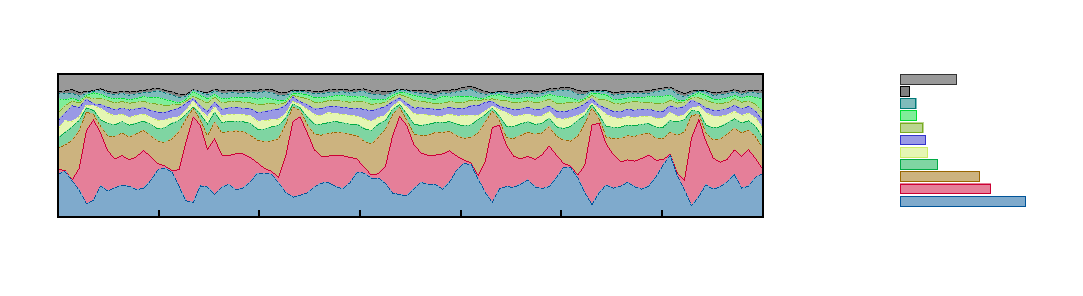
\includegraphics{img/day-es}}%
    \gplfronttext
  \end{picture}%
\endgroup


\noindent% GNUPLOT: LaTeX picture with Postscript
\begingroup
  \makeatletter
  \providecommand\color[2][]{%
    \GenericError{(gnuplot) \space\space\space\@spaces}{%
      Package color not loaded in conjunction with
      terminal option `colourtext'%
    }{See the gnuplot documentation for explanation.%
    }{Either use 'blacktext' in gnuplot or load the package
      color.sty in LaTeX.}%
    \renewcommand\color[2][]{}%
  }%
  \providecommand\includegraphics[2][]{%
    \GenericError{(gnuplot) \space\space\space\@spaces}{%
      Package graphicx or graphics not loaded%
    }{See the gnuplot documentation for explanation.%
    }{The gnuplot epslatex terminal needs graphicx.sty or graphics.sty.}%
    \renewcommand\includegraphics[2][]{}%
  }%
  \providecommand\rotatebox[2]{#2}%
  \@ifundefined{ifGPcolor}{%
    \newif\ifGPcolor
    \GPcolorfalse
  }{}%
  \@ifundefined{ifGPblacktext}{%
    \newif\ifGPblacktext
    \GPblacktexttrue
  }{}%
  % define a \g@addto@macro without @ in the name:
  \let\gplgaddtomacro\g@addto@macro
  % define empty templates for all commands taking text:
  \gdef\gplbacktext{}%
  \gdef\gplfronttext{}%
  \makeatother
  \ifGPblacktext
    % no textcolor at all
    \def\colorrgb#1{}%
    \def\colorgray#1{}%
  \else
    % gray or color?
    \ifGPcolor
      \def\colorrgb#1{\color[rgb]{#1}}%
      \def\colorgray#1{\color[gray]{#1}}%
      \expandafter\def\csname LTw\endcsname{\color{white}}%
      \expandafter\def\csname LTb\endcsname{\color{black}}%
      \expandafter\def\csname LTa\endcsname{\color{black}}%
      \expandafter\def\csname LT0\endcsname{\color[rgb]{1,0,0}}%
      \expandafter\def\csname LT1\endcsname{\color[rgb]{0,1,0}}%
      \expandafter\def\csname LT2\endcsname{\color[rgb]{0,0,1}}%
      \expandafter\def\csname LT3\endcsname{\color[rgb]{1,0,1}}%
      \expandafter\def\csname LT4\endcsname{\color[rgb]{0,1,1}}%
      \expandafter\def\csname LT5\endcsname{\color[rgb]{1,1,0}}%
      \expandafter\def\csname LT6\endcsname{\color[rgb]{0,0,0}}%
      \expandafter\def\csname LT7\endcsname{\color[rgb]{1,0.3,0}}%
      \expandafter\def\csname LT8\endcsname{\color[rgb]{0.5,0.5,0.5}}%
    \else
      % gray
      \def\colorrgb#1{\color{black}}%
      \def\colorgray#1{\color[gray]{#1}}%
      \expandafter\def\csname LTw\endcsname{\color{white}}%
      \expandafter\def\csname LTb\endcsname{\color{black}}%
      \expandafter\def\csname LTa\endcsname{\color{black}}%
      \expandafter\def\csname LT0\endcsname{\color{black}}%
      \expandafter\def\csname LT1\endcsname{\color{black}}%
      \expandafter\def\csname LT2\endcsname{\color{black}}%
      \expandafter\def\csname LT3\endcsname{\color{black}}%
      \expandafter\def\csname LT4\endcsname{\color{black}}%
      \expandafter\def\csname LT5\endcsname{\color{black}}%
      \expandafter\def\csname LT6\endcsname{\color{black}}%
      \expandafter\def\csname LT7\endcsname{\color{black}}%
      \expandafter\def\csname LT8\endcsname{\color{black}}%
    \fi
  \fi
  \setlength{\unitlength}{0.0500bp}%
  \begin{picture}(10080.00,2520.00)%
    \gplgaddtomacro\gplbacktext{%
      \csname LTb\endcsname%
      \put(176,1281){\rotatebox{-270}{\makebox(0,0){\strut{}\scriptsize fraction of tweets}}}%
      \put(3779,154){\makebox(0,0){\strut{}\scriptsize day of week(UTC)}}%
      \put(3779,2189){\makebox(0,0){\strut{}Countries that Tweet in French}}%
    }%
    \gplgaddtomacro\gplfronttext{%
      \csname LTb\endcsname%
      \put(396,374){\makebox(0,0){\strut{}\scriptsize 0}}%
      \put(1363,374){\makebox(0,0){\strut{}\scriptsize 1}}%
      \put(2329,374){\makebox(0,0){\strut{}\scriptsize 2}}%
      \put(3296,374){\makebox(0,0){\strut{}\scriptsize 3}}%
      \put(4263,374){\makebox(0,0){\strut{}\scriptsize 4}}%
      \put(5230,374){\makebox(0,0){\strut{}\scriptsize 5}}%
      \put(6196,374){\makebox(0,0){\strut{}\scriptsize 6}}%
      \put(7163,374){\makebox(0,0){\strut{}\scriptsize 7}}%
    }%
    \gplgaddtomacro\gplbacktext{%
      \csname LTb\endcsname%
      \put(9083,154){\makebox(0,0){\strut{}~~}}%
      \put(9083,2189){\makebox(0,0){\strut{} }}%
    }%
    \gplgaddtomacro\gplfronttext{%
      \csname LTb\endcsname%
      \put(8352,751){\makebox(0,0)[r]{\strut{}\scriptsize~France}}%
      \put(8352,868){\makebox(0,0)[r]{\strut{}\scriptsize~USA}}%
      \put(8352,985){\makebox(0,0)[r]{\strut{}\scriptsize~Canada}}%
      \put(8352,1102){\makebox(0,0)[r]{\strut{}\scriptsize~Belgium}}%
      \put(8352,1219){\makebox(0,0)[r]{\strut{}\scriptsize~Brazil}}%
      \put(8352,1337){\makebox(0,0)[r]{\strut{}\scriptsize~UK}}%
      \put(8352,1454){\makebox(0,0)[r]{\strut{}\scriptsize~Spain}}%
      \put(8352,1571){\makebox(0,0)[r]{\strut{}\scriptsize~Switzerland}}%
      \put(8352,1688){\makebox(0,0)[r]{\strut{}\scriptsize~Cameroon}}%
      \put(8352,1805){\makebox(0,0)[r]{\strut{}\scriptsize~Cote~d'Ivoire}}%
      \put(8352,1922){\makebox(0,0)[r]{\strut{}\scriptsize~other}}%
    }%
    \gplbacktext
    \put(0,0){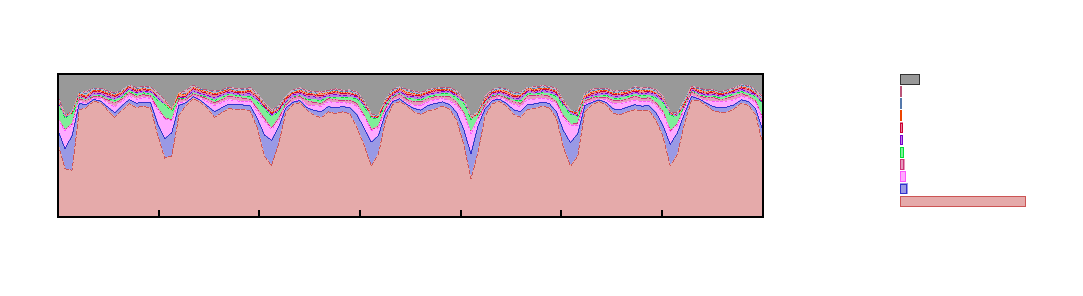
\includegraphics{img/day-fr}}%
    \gplfronttext
  \end{picture}%
\endgroup


\noindent% GNUPLOT: LaTeX picture with Postscript
\begingroup
  \makeatletter
  \providecommand\color[2][]{%
    \GenericError{(gnuplot) \space\space\space\@spaces}{%
      Package color not loaded in conjunction with
      terminal option `colourtext'%
    }{See the gnuplot documentation for explanation.%
    }{Either use 'blacktext' in gnuplot or load the package
      color.sty in LaTeX.}%
    \renewcommand\color[2][]{}%
  }%
  \providecommand\includegraphics[2][]{%
    \GenericError{(gnuplot) \space\space\space\@spaces}{%
      Package graphicx or graphics not loaded%
    }{See the gnuplot documentation for explanation.%
    }{The gnuplot epslatex terminal needs graphicx.sty or graphics.sty.}%
    \renewcommand\includegraphics[2][]{}%
  }%
  \providecommand\rotatebox[2]{#2}%
  \@ifundefined{ifGPcolor}{%
    \newif\ifGPcolor
    \GPcolorfalse
  }{}%
  \@ifundefined{ifGPblacktext}{%
    \newif\ifGPblacktext
    \GPblacktexttrue
  }{}%
  % define a \g@addto@macro without @ in the name:
  \let\gplgaddtomacro\g@addto@macro
  % define empty templates for all commands taking text:
  \gdef\gplbacktext{}%
  \gdef\gplfronttext{}%
  \makeatother
  \ifGPblacktext
    % no textcolor at all
    \def\colorrgb#1{}%
    \def\colorgray#1{}%
  \else
    % gray or color?
    \ifGPcolor
      \def\colorrgb#1{\color[rgb]{#1}}%
      \def\colorgray#1{\color[gray]{#1}}%
      \expandafter\def\csname LTw\endcsname{\color{white}}%
      \expandafter\def\csname LTb\endcsname{\color{black}}%
      \expandafter\def\csname LTa\endcsname{\color{black}}%
      \expandafter\def\csname LT0\endcsname{\color[rgb]{1,0,0}}%
      \expandafter\def\csname LT1\endcsname{\color[rgb]{0,1,0}}%
      \expandafter\def\csname LT2\endcsname{\color[rgb]{0,0,1}}%
      \expandafter\def\csname LT3\endcsname{\color[rgb]{1,0,1}}%
      \expandafter\def\csname LT4\endcsname{\color[rgb]{0,1,1}}%
      \expandafter\def\csname LT5\endcsname{\color[rgb]{1,1,0}}%
      \expandafter\def\csname LT6\endcsname{\color[rgb]{0,0,0}}%
      \expandafter\def\csname LT7\endcsname{\color[rgb]{1,0.3,0}}%
      \expandafter\def\csname LT8\endcsname{\color[rgb]{0.5,0.5,0.5}}%
    \else
      % gray
      \def\colorrgb#1{\color{black}}%
      \def\colorgray#1{\color[gray]{#1}}%
      \expandafter\def\csname LTw\endcsname{\color{white}}%
      \expandafter\def\csname LTb\endcsname{\color{black}}%
      \expandafter\def\csname LTa\endcsname{\color{black}}%
      \expandafter\def\csname LT0\endcsname{\color{black}}%
      \expandafter\def\csname LT1\endcsname{\color{black}}%
      \expandafter\def\csname LT2\endcsname{\color{black}}%
      \expandafter\def\csname LT3\endcsname{\color{black}}%
      \expandafter\def\csname LT4\endcsname{\color{black}}%
      \expandafter\def\csname LT5\endcsname{\color{black}}%
      \expandafter\def\csname LT6\endcsname{\color{black}}%
      \expandafter\def\csname LT7\endcsname{\color{black}}%
      \expandafter\def\csname LT8\endcsname{\color{black}}%
    \fi
  \fi
  \setlength{\unitlength}{0.0500bp}%
  \begin{picture}(10080.00,2520.00)%
    \gplgaddtomacro\gplbacktext{%
      \csname LTb\endcsname%
      \put(176,1281){\rotatebox{-270}{\makebox(0,0){\strut{}\scriptsize fraction of tweets}}}%
      \put(3779,154){\makebox(0,0){\strut{}\scriptsize day of week(UTC)}}%
      \put(3779,2189){\makebox(0,0){\strut{}Countries that Tweet in Indonesian}}%
    }%
    \gplgaddtomacro\gplfronttext{%
      \csname LTb\endcsname%
      \put(396,374){\makebox(0,0){\strut{}\scriptsize 0}}%
      \put(1363,374){\makebox(0,0){\strut{}\scriptsize 1}}%
      \put(2329,374){\makebox(0,0){\strut{}\scriptsize 2}}%
      \put(3296,374){\makebox(0,0){\strut{}\scriptsize 3}}%
      \put(4263,374){\makebox(0,0){\strut{}\scriptsize 4}}%
      \put(5230,374){\makebox(0,0){\strut{}\scriptsize 5}}%
      \put(6196,374){\makebox(0,0){\strut{}\scriptsize 6}}%
      \put(7163,374){\makebox(0,0){\strut{}\scriptsize 7}}%
    }%
    \gplgaddtomacro\gplbacktext{%
      \csname LTb\endcsname%
      \put(9083,154){\makebox(0,0){\strut{}~~}}%
      \put(9083,2189){\makebox(0,0){\strut{} }}%
    }%
    \gplgaddtomacro\gplfronttext{%
      \csname LTb\endcsname%
      \put(8352,751){\makebox(0,0)[r]{\strut{}\scriptsize~Malasia}}%
      \put(8352,868){\makebox(0,0)[r]{\strut{}\scriptsize~Indonesia}}%
      \put(8352,985){\makebox(0,0)[r]{\strut{}\scriptsize~Philippines}}%
      \put(8352,1102){\makebox(0,0)[r]{\strut{}\scriptsize~USA}}%
      \put(8352,1219){\makebox(0,0)[r]{\strut{}\scriptsize~Brazil}}%
      \put(8352,1337){\makebox(0,0)[r]{\strut{}\scriptsize~India}}%
      \put(8352,1454){\makebox(0,0)[r]{\strut{}\scriptsize~South~Africa}}%
      \put(8352,1571){\makebox(0,0)[r]{\strut{}\scriptsize~Thailand}}%
      \put(8352,1688){\makebox(0,0)[r]{\strut{}\scriptsize~Japan}}%
      \put(8352,1805){\makebox(0,0)[r]{\strut{}\scriptsize~TR}}%
      \put(8352,1922){\makebox(0,0)[r]{\strut{}\scriptsize~other}}%
    }%
    \gplbacktext
    \put(0,0){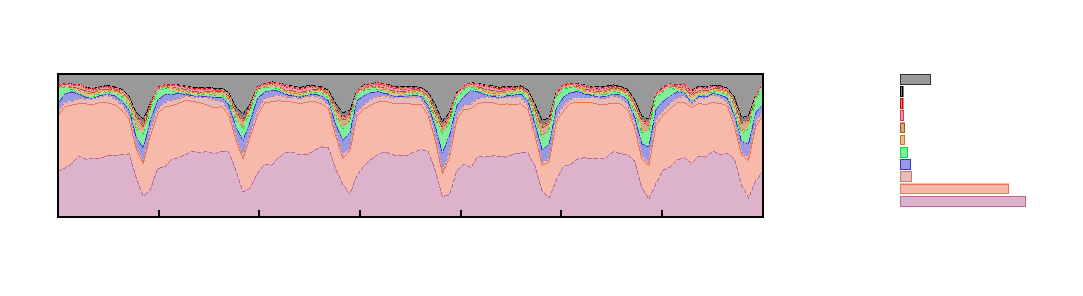
\includegraphics{img/day-in}}%
    \gplfronttext
  \end{picture}%
\endgroup


\noindent% GNUPLOT: LaTeX picture with Postscript
\begingroup
  \makeatletter
  \providecommand\color[2][]{%
    \GenericError{(gnuplot) \space\space\space\@spaces}{%
      Package color not loaded in conjunction with
      terminal option `colourtext'%
    }{See the gnuplot documentation for explanation.%
    }{Either use 'blacktext' in gnuplot or load the package
      color.sty in LaTeX.}%
    \renewcommand\color[2][]{}%
  }%
  \providecommand\includegraphics[2][]{%
    \GenericError{(gnuplot) \space\space\space\@spaces}{%
      Package graphicx or graphics not loaded%
    }{See the gnuplot documentation for explanation.%
    }{The gnuplot epslatex terminal needs graphicx.sty or graphics.sty.}%
    \renewcommand\includegraphics[2][]{}%
  }%
  \providecommand\rotatebox[2]{#2}%
  \@ifundefined{ifGPcolor}{%
    \newif\ifGPcolor
    \GPcolorfalse
  }{}%
  \@ifundefined{ifGPblacktext}{%
    \newif\ifGPblacktext
    \GPblacktexttrue
  }{}%
  % define a \g@addto@macro without @ in the name:
  \let\gplgaddtomacro\g@addto@macro
  % define empty templates for all commands taking text:
  \gdef\gplbacktext{}%
  \gdef\gplfronttext{}%
  \makeatother
  \ifGPblacktext
    % no textcolor at all
    \def\colorrgb#1{}%
    \def\colorgray#1{}%
  \else
    % gray or color?
    \ifGPcolor
      \def\colorrgb#1{\color[rgb]{#1}}%
      \def\colorgray#1{\color[gray]{#1}}%
      \expandafter\def\csname LTw\endcsname{\color{white}}%
      \expandafter\def\csname LTb\endcsname{\color{black}}%
      \expandafter\def\csname LTa\endcsname{\color{black}}%
      \expandafter\def\csname LT0\endcsname{\color[rgb]{1,0,0}}%
      \expandafter\def\csname LT1\endcsname{\color[rgb]{0,1,0}}%
      \expandafter\def\csname LT2\endcsname{\color[rgb]{0,0,1}}%
      \expandafter\def\csname LT3\endcsname{\color[rgb]{1,0,1}}%
      \expandafter\def\csname LT4\endcsname{\color[rgb]{0,1,1}}%
      \expandafter\def\csname LT5\endcsname{\color[rgb]{1,1,0}}%
      \expandafter\def\csname LT6\endcsname{\color[rgb]{0,0,0}}%
      \expandafter\def\csname LT7\endcsname{\color[rgb]{1,0.3,0}}%
      \expandafter\def\csname LT8\endcsname{\color[rgb]{0.5,0.5,0.5}}%
    \else
      % gray
      \def\colorrgb#1{\color{black}}%
      \def\colorgray#1{\color[gray]{#1}}%
      \expandafter\def\csname LTw\endcsname{\color{white}}%
      \expandafter\def\csname LTb\endcsname{\color{black}}%
      \expandafter\def\csname LTa\endcsname{\color{black}}%
      \expandafter\def\csname LT0\endcsname{\color{black}}%
      \expandafter\def\csname LT1\endcsname{\color{black}}%
      \expandafter\def\csname LT2\endcsname{\color{black}}%
      \expandafter\def\csname LT3\endcsname{\color{black}}%
      \expandafter\def\csname LT4\endcsname{\color{black}}%
      \expandafter\def\csname LT5\endcsname{\color{black}}%
      \expandafter\def\csname LT6\endcsname{\color{black}}%
      \expandafter\def\csname LT7\endcsname{\color{black}}%
      \expandafter\def\csname LT8\endcsname{\color{black}}%
    \fi
  \fi
  \setlength{\unitlength}{0.0500bp}%
  \begin{picture}(10080.00,2520.00)%
    \gplgaddtomacro\gplbacktext{%
      \csname LTb\endcsname%
      \put(176,1281){\rotatebox{-270}{\makebox(0,0){\strut{}\scriptsize fraction of tweets}}}%
      \put(3779,154){\makebox(0,0){\strut{}\scriptsize day of week(UTC)}}%
      \put(3779,2189){\makebox(0,0){\strut{}Countries that Tweet in Tagalog}}%
    }%
    \gplgaddtomacro\gplfronttext{%
      \csname LTb\endcsname%
      \put(396,374){\makebox(0,0){\strut{}\scriptsize 0}}%
      \put(1363,374){\makebox(0,0){\strut{}\scriptsize 1}}%
      \put(2329,374){\makebox(0,0){\strut{}\scriptsize 2}}%
      \put(3296,374){\makebox(0,0){\strut{}\scriptsize 3}}%
      \put(4263,374){\makebox(0,0){\strut{}\scriptsize 4}}%
      \put(5230,374){\makebox(0,0){\strut{}\scriptsize 5}}%
      \put(6196,374){\makebox(0,0){\strut{}\scriptsize 6}}%
      \put(7163,374){\makebox(0,0){\strut{}\scriptsize 7}}%
    }%
    \gplgaddtomacro\gplbacktext{%
      \csname LTb\endcsname%
      \put(9083,154){\makebox(0,0){\strut{}~~}}%
      \put(9083,2189){\makebox(0,0){\strut{} }}%
    }%
    \gplgaddtomacro\gplfronttext{%
      \csname LTb\endcsname%
      \put(8352,751){\makebox(0,0)[r]{\strut{}\scriptsize~Philippines}}%
      \put(8352,868){\makebox(0,0)[r]{\strut{}\scriptsize~USA}}%
      \put(8352,985){\makebox(0,0)[r]{\strut{}\scriptsize~Malasia}}%
      \put(8352,1102){\makebox(0,0)[r]{\strut{}\scriptsize~Brazil}}%
      \put(8352,1219){\makebox(0,0)[r]{\strut{}\scriptsize~Indonesia}}%
      \put(8352,1337){\makebox(0,0)[r]{\strut{}\scriptsize~South~Africa}}%
      \put(8352,1454){\makebox(0,0)[r]{\strut{}\scriptsize~India}}%
      \put(8352,1571){\makebox(0,0)[r]{\strut{}\scriptsize~UK}}%
      \put(8352,1688){\makebox(0,0)[r]{\strut{}\scriptsize~Canada}}%
      \put(8352,1805){\makebox(0,0)[r]{\strut{}\scriptsize~Japan}}%
      \put(8352,1922){\makebox(0,0)[r]{\strut{}\scriptsize~other}}%
    }%
    \gplbacktext
    \put(0,0){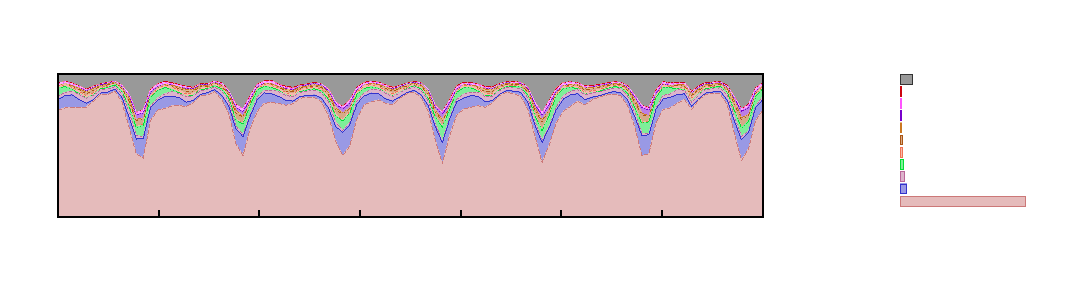
\includegraphics{img/day-tl}}%
    \gplfronttext
  \end{picture}%
\endgroup


\noindent% GNUPLOT: LaTeX picture with Postscript
\begingroup
  \makeatletter
  \providecommand\color[2][]{%
    \GenericError{(gnuplot) \space\space\space\@spaces}{%
      Package color not loaded in conjunction with
      terminal option `colourtext'%
    }{See the gnuplot documentation for explanation.%
    }{Either use 'blacktext' in gnuplot or load the package
      color.sty in LaTeX.}%
    \renewcommand\color[2][]{}%
  }%
  \providecommand\includegraphics[2][]{%
    \GenericError{(gnuplot) \space\space\space\@spaces}{%
      Package graphicx or graphics not loaded%
    }{See the gnuplot documentation for explanation.%
    }{The gnuplot epslatex terminal needs graphicx.sty or graphics.sty.}%
    \renewcommand\includegraphics[2][]{}%
  }%
  \providecommand\rotatebox[2]{#2}%
  \@ifundefined{ifGPcolor}{%
    \newif\ifGPcolor
    \GPcolorfalse
  }{}%
  \@ifundefined{ifGPblacktext}{%
    \newif\ifGPblacktext
    \GPblacktexttrue
  }{}%
  % define a \g@addto@macro without @ in the name:
  \let\gplgaddtomacro\g@addto@macro
  % define empty templates for all commands taking text:
  \gdef\gplbacktext{}%
  \gdef\gplfronttext{}%
  \makeatother
  \ifGPblacktext
    % no textcolor at all
    \def\colorrgb#1{}%
    \def\colorgray#1{}%
  \else
    % gray or color?
    \ifGPcolor
      \def\colorrgb#1{\color[rgb]{#1}}%
      \def\colorgray#1{\color[gray]{#1}}%
      \expandafter\def\csname LTw\endcsname{\color{white}}%
      \expandafter\def\csname LTb\endcsname{\color{black}}%
      \expandafter\def\csname LTa\endcsname{\color{black}}%
      \expandafter\def\csname LT0\endcsname{\color[rgb]{1,0,0}}%
      \expandafter\def\csname LT1\endcsname{\color[rgb]{0,1,0}}%
      \expandafter\def\csname LT2\endcsname{\color[rgb]{0,0,1}}%
      \expandafter\def\csname LT3\endcsname{\color[rgb]{1,0,1}}%
      \expandafter\def\csname LT4\endcsname{\color[rgb]{0,1,1}}%
      \expandafter\def\csname LT5\endcsname{\color[rgb]{1,1,0}}%
      \expandafter\def\csname LT6\endcsname{\color[rgb]{0,0,0}}%
      \expandafter\def\csname LT7\endcsname{\color[rgb]{1,0.3,0}}%
      \expandafter\def\csname LT8\endcsname{\color[rgb]{0.5,0.5,0.5}}%
    \else
      % gray
      \def\colorrgb#1{\color{black}}%
      \def\colorgray#1{\color[gray]{#1}}%
      \expandafter\def\csname LTw\endcsname{\color{white}}%
      \expandafter\def\csname LTb\endcsname{\color{black}}%
      \expandafter\def\csname LTa\endcsname{\color{black}}%
      \expandafter\def\csname LT0\endcsname{\color{black}}%
      \expandafter\def\csname LT1\endcsname{\color{black}}%
      \expandafter\def\csname LT2\endcsname{\color{black}}%
      \expandafter\def\csname LT3\endcsname{\color{black}}%
      \expandafter\def\csname LT4\endcsname{\color{black}}%
      \expandafter\def\csname LT5\endcsname{\color{black}}%
      \expandafter\def\csname LT6\endcsname{\color{black}}%
      \expandafter\def\csname LT7\endcsname{\color{black}}%
      \expandafter\def\csname LT8\endcsname{\color{black}}%
    \fi
  \fi
  \setlength{\unitlength}{0.0500bp}%
  \begin{picture}(10080.00,2520.00)%
    \gplgaddtomacro\gplbacktext{%
      \csname LTb\endcsname%
      \put(176,1281){\rotatebox{-270}{\makebox(0,0){\strut{}\scriptsize fraction of tweets}}}%
      \put(3779,154){\makebox(0,0){\strut{}\scriptsize day of week(UTC)}}%
      \put(3779,2189){\makebox(0,0){\strut{}Countries that Tweet in Turkish}}%
    }%
    \gplgaddtomacro\gplfronttext{%
      \csname LTb\endcsname%
      \put(396,374){\makebox(0,0){\strut{}\scriptsize 0}}%
      \put(1363,374){\makebox(0,0){\strut{}\scriptsize 1}}%
      \put(2329,374){\makebox(0,0){\strut{}\scriptsize 2}}%
      \put(3296,374){\makebox(0,0){\strut{}\scriptsize 3}}%
      \put(4263,374){\makebox(0,0){\strut{}\scriptsize 4}}%
      \put(5230,374){\makebox(0,0){\strut{}\scriptsize 5}}%
      \put(6196,374){\makebox(0,0){\strut{}\scriptsize 6}}%
      \put(7163,374){\makebox(0,0){\strut{}\scriptsize 7}}%
    }%
    \gplgaddtomacro\gplbacktext{%
      \csname LTb\endcsname%
      \put(9083,154){\makebox(0,0){\strut{}~~}}%
      \put(9083,2189){\makebox(0,0){\strut{} }}%
    }%
    \gplgaddtomacro\gplfronttext{%
      \csname LTb\endcsname%
      \put(8352,751){\makebox(0,0)[r]{\strut{}\scriptsize~TR}}%
      \put(8352,868){\makebox(0,0)[r]{\strut{}\scriptsize~USA}}%
      \put(8352,985){\makebox(0,0)[r]{\strut{}\scriptsize~DE}}%
      \put(8352,1102){\makebox(0,0)[r]{\strut{}\scriptsize~CY}}%
      \put(8352,1219){\makebox(0,0)[r]{\strut{}\scriptsize~AZ}}%
      \put(8352,1337){\makebox(0,0)[r]{\strut{}\scriptsize~Brazil}}%
      \put(8352,1454){\makebox(0,0)[r]{\strut{}\scriptsize~France}}%
      \put(8352,1571){\makebox(0,0)[r]{\strut{}\scriptsize~geo}}%
      \put(8352,1688){\makebox(0,0)[r]{\strut{}\scriptsize~UK}}%
      \put(8352,1805){\makebox(0,0)[r]{\strut{}\scriptsize~Philippines}}%
      \put(8352,1922){\makebox(0,0)[r]{\strut{}\scriptsize~other}}%
    }%
    \gplbacktext
    \put(0,0){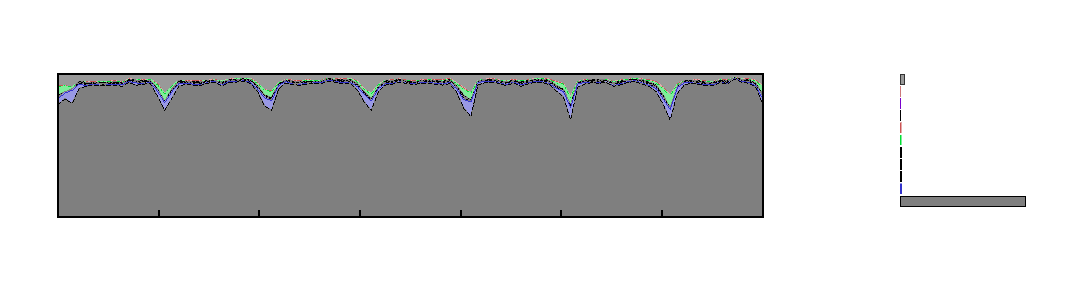
\includegraphics{img/day-tr}}%
    \gplfronttext
  \end{picture}%
\endgroup


\noindent% GNUPLOT: LaTeX picture with Postscript
\begingroup
  \makeatletter
  \providecommand\color[2][]{%
    \GenericError{(gnuplot) \space\space\space\@spaces}{%
      Package color not loaded in conjunction with
      terminal option `colourtext'%
    }{See the gnuplot documentation for explanation.%
    }{Either use 'blacktext' in gnuplot or load the package
      color.sty in LaTeX.}%
    \renewcommand\color[2][]{}%
  }%
  \providecommand\includegraphics[2][]{%
    \GenericError{(gnuplot) \space\space\space\@spaces}{%
      Package graphicx or graphics not loaded%
    }{See the gnuplot documentation for explanation.%
    }{The gnuplot epslatex terminal needs graphicx.sty or graphics.sty.}%
    \renewcommand\includegraphics[2][]{}%
  }%
  \providecommand\rotatebox[2]{#2}%
  \@ifundefined{ifGPcolor}{%
    \newif\ifGPcolor
    \GPcolorfalse
  }{}%
  \@ifundefined{ifGPblacktext}{%
    \newif\ifGPblacktext
    \GPblacktexttrue
  }{}%
  % define a \g@addto@macro without @ in the name:
  \let\gplgaddtomacro\g@addto@macro
  % define empty templates for all commands taking text:
  \gdef\gplbacktext{}%
  \gdef\gplfronttext{}%
  \makeatother
  \ifGPblacktext
    % no textcolor at all
    \def\colorrgb#1{}%
    \def\colorgray#1{}%
  \else
    % gray or color?
    \ifGPcolor
      \def\colorrgb#1{\color[rgb]{#1}}%
      \def\colorgray#1{\color[gray]{#1}}%
      \expandafter\def\csname LTw\endcsname{\color{white}}%
      \expandafter\def\csname LTb\endcsname{\color{black}}%
      \expandafter\def\csname LTa\endcsname{\color{black}}%
      \expandafter\def\csname LT0\endcsname{\color[rgb]{1,0,0}}%
      \expandafter\def\csname LT1\endcsname{\color[rgb]{0,1,0}}%
      \expandafter\def\csname LT2\endcsname{\color[rgb]{0,0,1}}%
      \expandafter\def\csname LT3\endcsname{\color[rgb]{1,0,1}}%
      \expandafter\def\csname LT4\endcsname{\color[rgb]{0,1,1}}%
      \expandafter\def\csname LT5\endcsname{\color[rgb]{1,1,0}}%
      \expandafter\def\csname LT6\endcsname{\color[rgb]{0,0,0}}%
      \expandafter\def\csname LT7\endcsname{\color[rgb]{1,0.3,0}}%
      \expandafter\def\csname LT8\endcsname{\color[rgb]{0.5,0.5,0.5}}%
    \else
      % gray
      \def\colorrgb#1{\color{black}}%
      \def\colorgray#1{\color[gray]{#1}}%
      \expandafter\def\csname LTw\endcsname{\color{white}}%
      \expandafter\def\csname LTb\endcsname{\color{black}}%
      \expandafter\def\csname LTa\endcsname{\color{black}}%
      \expandafter\def\csname LT0\endcsname{\color{black}}%
      \expandafter\def\csname LT1\endcsname{\color{black}}%
      \expandafter\def\csname LT2\endcsname{\color{black}}%
      \expandafter\def\csname LT3\endcsname{\color{black}}%
      \expandafter\def\csname LT4\endcsname{\color{black}}%
      \expandafter\def\csname LT5\endcsname{\color{black}}%
      \expandafter\def\csname LT6\endcsname{\color{black}}%
      \expandafter\def\csname LT7\endcsname{\color{black}}%
      \expandafter\def\csname LT8\endcsname{\color{black}}%
    \fi
  \fi
  \setlength{\unitlength}{0.0500bp}%
  \begin{picture}(10080.00,2520.00)%
    \gplgaddtomacro\gplbacktext{%
      \csname LTb\endcsname%
      \put(176,1281){\rotatebox{-270}{\makebox(0,0){\strut{}\scriptsize fraction of tweets}}}%
      \put(3779,154){\makebox(0,0){\strut{}\scriptsize day of week(UTC)}}%
      \put(3779,2189){\makebox(0,0){\strut{}Countries that Tweet in Japanese}}%
    }%
    \gplgaddtomacro\gplfronttext{%
      \csname LTb\endcsname%
      \put(396,374){\makebox(0,0){\strut{}\scriptsize 0}}%
      \put(1363,374){\makebox(0,0){\strut{}\scriptsize 1}}%
      \put(2329,374){\makebox(0,0){\strut{}\scriptsize 2}}%
      \put(3296,374){\makebox(0,0){\strut{}\scriptsize 3}}%
      \put(4263,374){\makebox(0,0){\strut{}\scriptsize 4}}%
      \put(5230,374){\makebox(0,0){\strut{}\scriptsize 5}}%
      \put(6196,374){\makebox(0,0){\strut{}\scriptsize 6}}%
      \put(7163,374){\makebox(0,0){\strut{}\scriptsize 7}}%
    }%
    \gplgaddtomacro\gplbacktext{%
      \csname LTb\endcsname%
      \put(9083,154){\makebox(0,0){\strut{}~~}}%
      \put(9083,2189){\makebox(0,0){\strut{} }}%
    }%
    \gplgaddtomacro\gplfronttext{%
      \csname LTb\endcsname%
      \put(8352,751){\makebox(0,0)[r]{\strut{}\scriptsize~Japan}}%
      \put(8352,868){\makebox(0,0)[r]{\strut{}\scriptsize~USA}}%
      \put(8352,985){\makebox(0,0)[r]{\strut{}\scriptsize~Taiwan}}%
      \put(8352,1102){\makebox(0,0)[r]{\strut{}\scriptsize~China}}%
      \put(8352,1219){\makebox(0,0)[r]{\strut{}\scriptsize~South~Korea}}%
      \put(8352,1337){\makebox(0,0)[r]{\strut{}\scriptsize~Thailand}}%
      \put(8352,1454){\makebox(0,0)[r]{\strut{}\scriptsize~Hong~Kong}}%
      \put(8352,1571){\makebox(0,0)[r]{\strut{}\scriptsize~Australia}}%
      \put(8352,1688){\makebox(0,0)[r]{\strut{}\scriptsize~Canada}}%
      \put(8352,1805){\makebox(0,0)[r]{\strut{}\scriptsize~Malasia}}%
      \put(8352,1922){\makebox(0,0)[r]{\strut{}\scriptsize~other}}%
    }%
    \gplbacktext
    \put(0,0){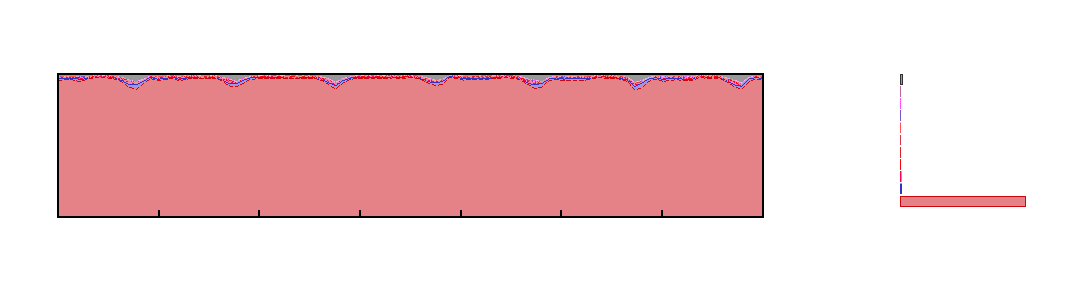
\includegraphics{img/day-ja}}%
    \gplfronttext
  \end{picture}%
\endgroup


\noindent% GNUPLOT: LaTeX picture with Postscript
\begingroup
  \makeatletter
  \providecommand\color[2][]{%
    \GenericError{(gnuplot) \space\space\space\@spaces}{%
      Package color not loaded in conjunction with
      terminal option `colourtext'%
    }{See the gnuplot documentation for explanation.%
    }{Either use 'blacktext' in gnuplot or load the package
      color.sty in LaTeX.}%
    \renewcommand\color[2][]{}%
  }%
  \providecommand\includegraphics[2][]{%
    \GenericError{(gnuplot) \space\space\space\@spaces}{%
      Package graphicx or graphics not loaded%
    }{See the gnuplot documentation for explanation.%
    }{The gnuplot epslatex terminal needs graphicx.sty or graphics.sty.}%
    \renewcommand\includegraphics[2][]{}%
  }%
  \providecommand\rotatebox[2]{#2}%
  \@ifundefined{ifGPcolor}{%
    \newif\ifGPcolor
    \GPcolorfalse
  }{}%
  \@ifundefined{ifGPblacktext}{%
    \newif\ifGPblacktext
    \GPblacktexttrue
  }{}%
  % define a \g@addto@macro without @ in the name:
  \let\gplgaddtomacro\g@addto@macro
  % define empty templates for all commands taking text:
  \gdef\gplbacktext{}%
  \gdef\gplfronttext{}%
  \makeatother
  \ifGPblacktext
    % no textcolor at all
    \def\colorrgb#1{}%
    \def\colorgray#1{}%
  \else
    % gray or color?
    \ifGPcolor
      \def\colorrgb#1{\color[rgb]{#1}}%
      \def\colorgray#1{\color[gray]{#1}}%
      \expandafter\def\csname LTw\endcsname{\color{white}}%
      \expandafter\def\csname LTb\endcsname{\color{black}}%
      \expandafter\def\csname LTa\endcsname{\color{black}}%
      \expandafter\def\csname LT0\endcsname{\color[rgb]{1,0,0}}%
      \expandafter\def\csname LT1\endcsname{\color[rgb]{0,1,0}}%
      \expandafter\def\csname LT2\endcsname{\color[rgb]{0,0,1}}%
      \expandafter\def\csname LT3\endcsname{\color[rgb]{1,0,1}}%
      \expandafter\def\csname LT4\endcsname{\color[rgb]{0,1,1}}%
      \expandafter\def\csname LT5\endcsname{\color[rgb]{1,1,0}}%
      \expandafter\def\csname LT6\endcsname{\color[rgb]{0,0,0}}%
      \expandafter\def\csname LT7\endcsname{\color[rgb]{1,0.3,0}}%
      \expandafter\def\csname LT8\endcsname{\color[rgb]{0.5,0.5,0.5}}%
    \else
      % gray
      \def\colorrgb#1{\color{black}}%
      \def\colorgray#1{\color[gray]{#1}}%
      \expandafter\def\csname LTw\endcsname{\color{white}}%
      \expandafter\def\csname LTb\endcsname{\color{black}}%
      \expandafter\def\csname LTa\endcsname{\color{black}}%
      \expandafter\def\csname LT0\endcsname{\color{black}}%
      \expandafter\def\csname LT1\endcsname{\color{black}}%
      \expandafter\def\csname LT2\endcsname{\color{black}}%
      \expandafter\def\csname LT3\endcsname{\color{black}}%
      \expandafter\def\csname LT4\endcsname{\color{black}}%
      \expandafter\def\csname LT5\endcsname{\color{black}}%
      \expandafter\def\csname LT6\endcsname{\color{black}}%
      \expandafter\def\csname LT7\endcsname{\color{black}}%
      \expandafter\def\csname LT8\endcsname{\color{black}}%
    \fi
  \fi
  \setlength{\unitlength}{0.0500bp}%
  \begin{picture}(10080.00,2520.00)%
    \gplgaddtomacro\gplbacktext{%
      \csname LTb\endcsname%
      \put(176,1281){\rotatebox{-270}{\makebox(0,0){\strut{}\scriptsize fraction of tweets}}}%
      \put(3779,154){\makebox(0,0){\strut{}\scriptsize day of week(UTC)}}%
      \put(3779,2189){\makebox(0,0){\strut{}Countries that Tweet in Korean}}%
    }%
    \gplgaddtomacro\gplfronttext{%
      \csname LTb\endcsname%
      \put(396,374){\makebox(0,0){\strut{}\scriptsize 0}}%
      \put(1363,374){\makebox(0,0){\strut{}\scriptsize 1}}%
      \put(2329,374){\makebox(0,0){\strut{}\scriptsize 2}}%
      \put(3296,374){\makebox(0,0){\strut{}\scriptsize 3}}%
      \put(4263,374){\makebox(0,0){\strut{}\scriptsize 4}}%
      \put(5230,374){\makebox(0,0){\strut{}\scriptsize 5}}%
      \put(6196,374){\makebox(0,0){\strut{}\scriptsize 6}}%
      \put(7163,374){\makebox(0,0){\strut{}\scriptsize 7}}%
    }%
    \gplgaddtomacro\gplbacktext{%
      \csname LTb\endcsname%
      \put(9083,154){\makebox(0,0){\strut{}~~}}%
      \put(9083,2189){\makebox(0,0){\strut{} }}%
    }%
    \gplgaddtomacro\gplfronttext{%
      \csname LTb\endcsname%
      \put(8352,751){\makebox(0,0)[r]{\strut{}\scriptsize~South~Korea}}%
      \put(8352,868){\makebox(0,0)[r]{\strut{}\scriptsize~Japan}}%
      \put(8352,985){\makebox(0,0)[r]{\strut{}\scriptsize~USA}}%
      \put(8352,1102){\makebox(0,0)[r]{\strut{}\scriptsize~Thailand}}%
      \put(8352,1219){\makebox(0,0)[r]{\strut{}\scriptsize~Philippines}}%
      \put(8352,1337){\makebox(0,0)[r]{\strut{}\scriptsize~Canada}}%
      \put(8352,1454){\makebox(0,0)[r]{\strut{}\scriptsize~Indonesia}}%
      \put(8352,1571){\makebox(0,0)[r]{\strut{}\scriptsize~DE}}%
      \put(8352,1688){\makebox(0,0)[r]{\strut{}\scriptsize~Brazil}}%
      \put(8352,1805){\makebox(0,0)[r]{\strut{}\scriptsize~Malasia}}%
      \put(8352,1922){\makebox(0,0)[r]{\strut{}\scriptsize~other}}%
    }%
    \gplbacktext
    \put(0,0){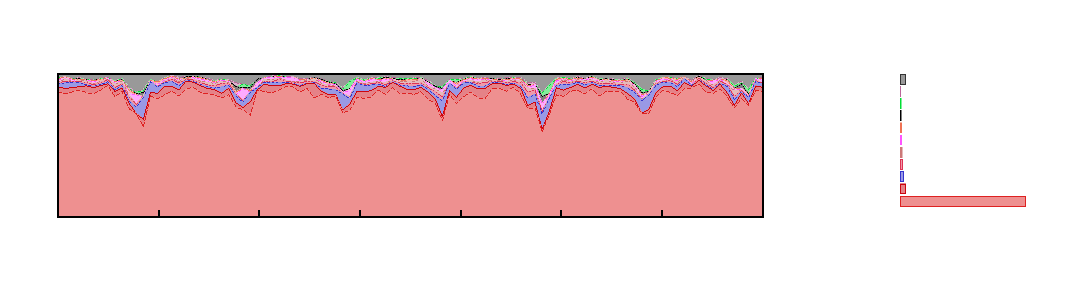
\includegraphics{img/day-ko}}%
    \gplfronttext
  \end{picture}%
\endgroup


\noindent% GNUPLOT: LaTeX picture with Postscript
\begingroup
  \makeatletter
  \providecommand\color[2][]{%
    \GenericError{(gnuplot) \space\space\space\@spaces}{%
      Package color not loaded in conjunction with
      terminal option `colourtext'%
    }{See the gnuplot documentation for explanation.%
    }{Either use 'blacktext' in gnuplot or load the package
      color.sty in LaTeX.}%
    \renewcommand\color[2][]{}%
  }%
  \providecommand\includegraphics[2][]{%
    \GenericError{(gnuplot) \space\space\space\@spaces}{%
      Package graphicx or graphics not loaded%
    }{See the gnuplot documentation for explanation.%
    }{The gnuplot epslatex terminal needs graphicx.sty or graphics.sty.}%
    \renewcommand\includegraphics[2][]{}%
  }%
  \providecommand\rotatebox[2]{#2}%
  \@ifundefined{ifGPcolor}{%
    \newif\ifGPcolor
    \GPcolorfalse
  }{}%
  \@ifundefined{ifGPblacktext}{%
    \newif\ifGPblacktext
    \GPblacktexttrue
  }{}%
  % define a \g@addto@macro without @ in the name:
  \let\gplgaddtomacro\g@addto@macro
  % define empty templates for all commands taking text:
  \gdef\gplbacktext{}%
  \gdef\gplfronttext{}%
  \makeatother
  \ifGPblacktext
    % no textcolor at all
    \def\colorrgb#1{}%
    \def\colorgray#1{}%
  \else
    % gray or color?
    \ifGPcolor
      \def\colorrgb#1{\color[rgb]{#1}}%
      \def\colorgray#1{\color[gray]{#1}}%
      \expandafter\def\csname LTw\endcsname{\color{white}}%
      \expandafter\def\csname LTb\endcsname{\color{black}}%
      \expandafter\def\csname LTa\endcsname{\color{black}}%
      \expandafter\def\csname LT0\endcsname{\color[rgb]{1,0,0}}%
      \expandafter\def\csname LT1\endcsname{\color[rgb]{0,1,0}}%
      \expandafter\def\csname LT2\endcsname{\color[rgb]{0,0,1}}%
      \expandafter\def\csname LT3\endcsname{\color[rgb]{1,0,1}}%
      \expandafter\def\csname LT4\endcsname{\color[rgb]{0,1,1}}%
      \expandafter\def\csname LT5\endcsname{\color[rgb]{1,1,0}}%
      \expandafter\def\csname LT6\endcsname{\color[rgb]{0,0,0}}%
      \expandafter\def\csname LT7\endcsname{\color[rgb]{1,0.3,0}}%
      \expandafter\def\csname LT8\endcsname{\color[rgb]{0.5,0.5,0.5}}%
    \else
      % gray
      \def\colorrgb#1{\color{black}}%
      \def\colorgray#1{\color[gray]{#1}}%
      \expandafter\def\csname LTw\endcsname{\color{white}}%
      \expandafter\def\csname LTb\endcsname{\color{black}}%
      \expandafter\def\csname LTa\endcsname{\color{black}}%
      \expandafter\def\csname LT0\endcsname{\color{black}}%
      \expandafter\def\csname LT1\endcsname{\color{black}}%
      \expandafter\def\csname LT2\endcsname{\color{black}}%
      \expandafter\def\csname LT3\endcsname{\color{black}}%
      \expandafter\def\csname LT4\endcsname{\color{black}}%
      \expandafter\def\csname LT5\endcsname{\color{black}}%
      \expandafter\def\csname LT6\endcsname{\color{black}}%
      \expandafter\def\csname LT7\endcsname{\color{black}}%
      \expandafter\def\csname LT8\endcsname{\color{black}}%
    \fi
  \fi
  \setlength{\unitlength}{0.0500bp}%
  \begin{picture}(10080.00,2520.00)%
    \gplgaddtomacro\gplbacktext{%
      \csname LTb\endcsname%
      \put(176,1281){\rotatebox{-270}{\makebox(0,0){\strut{}\scriptsize fraction of tweets}}}%
      \put(3779,154){\makebox(0,0){\strut{}\scriptsize day of week(UTC)}}%
      \put(3779,2189){\makebox(0,0){\strut{}Countries that Tweet in Portuguese}}%
    }%
    \gplgaddtomacro\gplfronttext{%
      \csname LTb\endcsname%
      \put(396,374){\makebox(0,0){\strut{}\scriptsize 0}}%
      \put(1363,374){\makebox(0,0){\strut{}\scriptsize 1}}%
      \put(2329,374){\makebox(0,0){\strut{}\scriptsize 2}}%
      \put(3296,374){\makebox(0,0){\strut{}\scriptsize 3}}%
      \put(4263,374){\makebox(0,0){\strut{}\scriptsize 4}}%
      \put(5230,374){\makebox(0,0){\strut{}\scriptsize 5}}%
      \put(6196,374){\makebox(0,0){\strut{}\scriptsize 6}}%
      \put(7163,374){\makebox(0,0){\strut{}\scriptsize 7}}%
    }%
    \gplgaddtomacro\gplbacktext{%
      \csname LTb\endcsname%
      \put(9083,154){\makebox(0,0){\strut{}~~}}%
      \put(9083,2189){\makebox(0,0){\strut{} }}%
    }%
    \gplgaddtomacro\gplfronttext{%
      \csname LTb\endcsname%
      \put(8352,751){\makebox(0,0)[r]{\strut{}\scriptsize~Brazil}}%
      \put(8352,868){\makebox(0,0)[r]{\strut{}\scriptsize~Portugal}}%
      \put(8352,985){\makebox(0,0)[r]{\strut{}\scriptsize~USA}}%
      \put(8352,1102){\makebox(0,0)[r]{\strut{}\scriptsize~Argentina}}%
      \put(8352,1219){\makebox(0,0)[r]{\strut{}\scriptsize~Spain}}%
      \put(8352,1337){\makebox(0,0)[r]{\strut{}\scriptsize~Mexico}}%
      \put(8352,1454){\makebox(0,0)[r]{\strut{}\scriptsize~UK}}%
      \put(8352,1571){\makebox(0,0)[r]{\strut{}\scriptsize~France}}%
      \put(8352,1688){\makebox(0,0)[r]{\strut{}\scriptsize~Italy}}%
      \put(8352,1805){\makebox(0,0)[r]{\strut{}\scriptsize~Uruguay}}%
      \put(8352,1922){\makebox(0,0)[r]{\strut{}\scriptsize~other}}%
    }%
    \gplbacktext
    \put(0,0){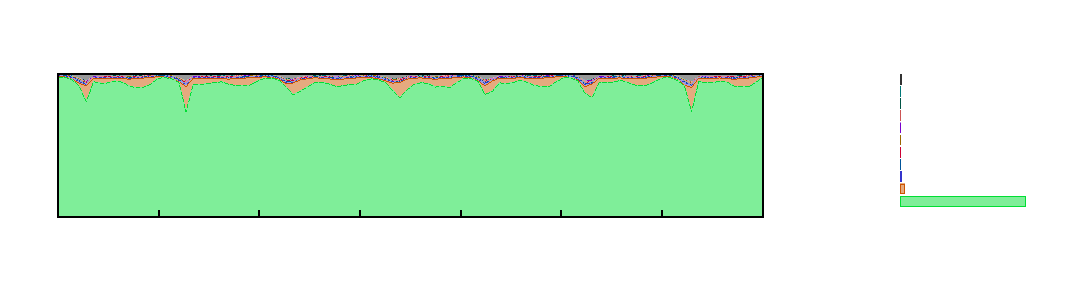
\includegraphics{img/day-pt}}%
    \gplfronttext
  \end{picture}%
\endgroup


\noindent% GNUPLOT: LaTeX picture with Postscript
\begingroup
  \makeatletter
  \providecommand\color[2][]{%
    \GenericError{(gnuplot) \space\space\space\@spaces}{%
      Package color not loaded in conjunction with
      terminal option `colourtext'%
    }{See the gnuplot documentation for explanation.%
    }{Either use 'blacktext' in gnuplot or load the package
      color.sty in LaTeX.}%
    \renewcommand\color[2][]{}%
  }%
  \providecommand\includegraphics[2][]{%
    \GenericError{(gnuplot) \space\space\space\@spaces}{%
      Package graphicx or graphics not loaded%
    }{See the gnuplot documentation for explanation.%
    }{The gnuplot epslatex terminal needs graphicx.sty or graphics.sty.}%
    \renewcommand\includegraphics[2][]{}%
  }%
  \providecommand\rotatebox[2]{#2}%
  \@ifundefined{ifGPcolor}{%
    \newif\ifGPcolor
    \GPcolorfalse
  }{}%
  \@ifundefined{ifGPblacktext}{%
    \newif\ifGPblacktext
    \GPblacktexttrue
  }{}%
  % define a \g@addto@macro without @ in the name:
  \let\gplgaddtomacro\g@addto@macro
  % define empty templates for all commands taking text:
  \gdef\gplbacktext{}%
  \gdef\gplfronttext{}%
  \makeatother
  \ifGPblacktext
    % no textcolor at all
    \def\colorrgb#1{}%
    \def\colorgray#1{}%
  \else
    % gray or color?
    \ifGPcolor
      \def\colorrgb#1{\color[rgb]{#1}}%
      \def\colorgray#1{\color[gray]{#1}}%
      \expandafter\def\csname LTw\endcsname{\color{white}}%
      \expandafter\def\csname LTb\endcsname{\color{black}}%
      \expandafter\def\csname LTa\endcsname{\color{black}}%
      \expandafter\def\csname LT0\endcsname{\color[rgb]{1,0,0}}%
      \expandafter\def\csname LT1\endcsname{\color[rgb]{0,1,0}}%
      \expandafter\def\csname LT2\endcsname{\color[rgb]{0,0,1}}%
      \expandafter\def\csname LT3\endcsname{\color[rgb]{1,0,1}}%
      \expandafter\def\csname LT4\endcsname{\color[rgb]{0,1,1}}%
      \expandafter\def\csname LT5\endcsname{\color[rgb]{1,1,0}}%
      \expandafter\def\csname LT6\endcsname{\color[rgb]{0,0,0}}%
      \expandafter\def\csname LT7\endcsname{\color[rgb]{1,0.3,0}}%
      \expandafter\def\csname LT8\endcsname{\color[rgb]{0.5,0.5,0.5}}%
    \else
      % gray
      \def\colorrgb#1{\color{black}}%
      \def\colorgray#1{\color[gray]{#1}}%
      \expandafter\def\csname LTw\endcsname{\color{white}}%
      \expandafter\def\csname LTb\endcsname{\color{black}}%
      \expandafter\def\csname LTa\endcsname{\color{black}}%
      \expandafter\def\csname LT0\endcsname{\color{black}}%
      \expandafter\def\csname LT1\endcsname{\color{black}}%
      \expandafter\def\csname LT2\endcsname{\color{black}}%
      \expandafter\def\csname LT3\endcsname{\color{black}}%
      \expandafter\def\csname LT4\endcsname{\color{black}}%
      \expandafter\def\csname LT5\endcsname{\color{black}}%
      \expandafter\def\csname LT6\endcsname{\color{black}}%
      \expandafter\def\csname LT7\endcsname{\color{black}}%
      \expandafter\def\csname LT8\endcsname{\color{black}}%
    \fi
  \fi
  \setlength{\unitlength}{0.0500bp}%
  \begin{picture}(10080.00,2520.00)%
    \gplgaddtomacro\gplbacktext{%
      \csname LTb\endcsname%
      \put(176,1281){\rotatebox{-270}{\makebox(0,0){\strut{}\scriptsize fraction of tweets}}}%
      \put(3779,154){\makebox(0,0){\strut{}\scriptsize day of week(UTC)}}%
      \put(3779,2189){\makebox(0,0){\strut{}Countries that Tweet in Chinese}}%
    }%
    \gplgaddtomacro\gplfronttext{%
      \csname LTb\endcsname%
      \put(396,374){\makebox(0,0){\strut{}\scriptsize 0}}%
      \put(1363,374){\makebox(0,0){\strut{}\scriptsize 1}}%
      \put(2329,374){\makebox(0,0){\strut{}\scriptsize 2}}%
      \put(3296,374){\makebox(0,0){\strut{}\scriptsize 3}}%
      \put(4263,374){\makebox(0,0){\strut{}\scriptsize 4}}%
      \put(5230,374){\makebox(0,0){\strut{}\scriptsize 5}}%
      \put(6196,374){\makebox(0,0){\strut{}\scriptsize 6}}%
      \put(7163,374){\makebox(0,0){\strut{}\scriptsize 7}}%
    }%
    \gplgaddtomacro\gplbacktext{%
      \csname LTb\endcsname%
      \put(9083,154){\makebox(0,0){\strut{}~~}}%
      \put(9083,2189){\makebox(0,0){\strut{} }}%
    }%
    \gplgaddtomacro\gplfronttext{%
      \csname LTb\endcsname%
      \put(8352,751){\makebox(0,0)[r]{\strut{}\scriptsize~China}}%
      \put(8352,868){\makebox(0,0)[r]{\strut{}\scriptsize~Taiwan}}%
      \put(8352,985){\makebox(0,0)[r]{\strut{}\scriptsize~USA}}%
      \put(8352,1102){\makebox(0,0)[r]{\strut{}\scriptsize~Japan}}%
      \put(8352,1219){\makebox(0,0)[r]{\strut{}\scriptsize~Malasia}}%
      \put(8352,1337){\makebox(0,0)[r]{\strut{}\scriptsize~Hong~Kong}}%
      \put(8352,1454){\makebox(0,0)[r]{\strut{}\scriptsize~Canada}}%
      \put(8352,1571){\makebox(0,0)[r]{\strut{}\scriptsize~Australia}}%
      \put(8352,1688){\makebox(0,0)[r]{\strut{}\scriptsize~Singapore}}%
      \put(8352,1805){\makebox(0,0)[r]{\strut{}\scriptsize~UK}}%
      \put(8352,1922){\makebox(0,0)[r]{\strut{}\scriptsize~other}}%
    }%
    \gplbacktext
    \put(0,0){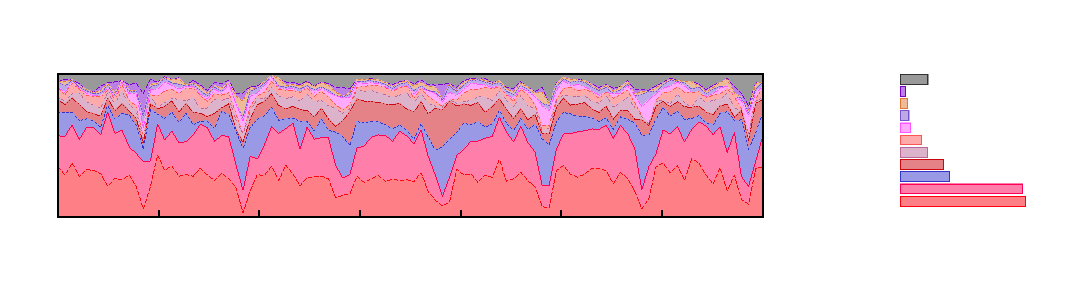
\includegraphics{img/day-zh}}%
    \gplfronttext
  \end{picture}%
\endgroup


\noindent% GNUPLOT: LaTeX picture with Postscript
\begingroup
  \makeatletter
  \providecommand\color[2][]{%
    \GenericError{(gnuplot) \space\space\space\@spaces}{%
      Package color not loaded in conjunction with
      terminal option `colourtext'%
    }{See the gnuplot documentation for explanation.%
    }{Either use 'blacktext' in gnuplot or load the package
      color.sty in LaTeX.}%
    \renewcommand\color[2][]{}%
  }%
  \providecommand\includegraphics[2][]{%
    \GenericError{(gnuplot) \space\space\space\@spaces}{%
      Package graphicx or graphics not loaded%
    }{See the gnuplot documentation for explanation.%
    }{The gnuplot epslatex terminal needs graphicx.sty or graphics.sty.}%
    \renewcommand\includegraphics[2][]{}%
  }%
  \providecommand\rotatebox[2]{#2}%
  \@ifundefined{ifGPcolor}{%
    \newif\ifGPcolor
    \GPcolorfalse
  }{}%
  \@ifundefined{ifGPblacktext}{%
    \newif\ifGPblacktext
    \GPblacktexttrue
  }{}%
  % define a \g@addto@macro without @ in the name:
  \let\gplgaddtomacro\g@addto@macro
  % define empty templates for all commands taking text:
  \gdef\gplbacktext{}%
  \gdef\gplfronttext{}%
  \makeatother
  \ifGPblacktext
    % no textcolor at all
    \def\colorrgb#1{}%
    \def\colorgray#1{}%
  \else
    % gray or color?
    \ifGPcolor
      \def\colorrgb#1{\color[rgb]{#1}}%
      \def\colorgray#1{\color[gray]{#1}}%
      \expandafter\def\csname LTw\endcsname{\color{white}}%
      \expandafter\def\csname LTb\endcsname{\color{black}}%
      \expandafter\def\csname LTa\endcsname{\color{black}}%
      \expandafter\def\csname LT0\endcsname{\color[rgb]{1,0,0}}%
      \expandafter\def\csname LT1\endcsname{\color[rgb]{0,1,0}}%
      \expandafter\def\csname LT2\endcsname{\color[rgb]{0,0,1}}%
      \expandafter\def\csname LT3\endcsname{\color[rgb]{1,0,1}}%
      \expandafter\def\csname LT4\endcsname{\color[rgb]{0,1,1}}%
      \expandafter\def\csname LT5\endcsname{\color[rgb]{1,1,0}}%
      \expandafter\def\csname LT6\endcsname{\color[rgb]{0,0,0}}%
      \expandafter\def\csname LT7\endcsname{\color[rgb]{1,0.3,0}}%
      \expandafter\def\csname LT8\endcsname{\color[rgb]{0.5,0.5,0.5}}%
    \else
      % gray
      \def\colorrgb#1{\color{black}}%
      \def\colorgray#1{\color[gray]{#1}}%
      \expandafter\def\csname LTw\endcsname{\color{white}}%
      \expandafter\def\csname LTb\endcsname{\color{black}}%
      \expandafter\def\csname LTa\endcsname{\color{black}}%
      \expandafter\def\csname LT0\endcsname{\color{black}}%
      \expandafter\def\csname LT1\endcsname{\color{black}}%
      \expandafter\def\csname LT2\endcsname{\color{black}}%
      \expandafter\def\csname LT3\endcsname{\color{black}}%
      \expandafter\def\csname LT4\endcsname{\color{black}}%
      \expandafter\def\csname LT5\endcsname{\color{black}}%
      \expandafter\def\csname LT6\endcsname{\color{black}}%
      \expandafter\def\csname LT7\endcsname{\color{black}}%
      \expandafter\def\csname LT8\endcsname{\color{black}}%
    \fi
  \fi
  \setlength{\unitlength}{0.0500bp}%
  \begin{picture}(10080.00,2520.00)%
    \gplgaddtomacro\gplbacktext{%
      \csname LTb\endcsname%
      \put(176,1281){\rotatebox{-270}{\makebox(0,0){\strut{}\scriptsize fraction of tweets}}}%
      \put(3779,154){\makebox(0,0){\strut{}\scriptsize day of week(UTC)}}%
      \put(3779,2189){\makebox(0,0){\strut{}Countries that Tweet in und}}%
    }%
    \gplgaddtomacro\gplfronttext{%
      \csname LTb\endcsname%
      \put(396,374){\makebox(0,0){\strut{}\scriptsize 0}}%
      \put(1363,374){\makebox(0,0){\strut{}\scriptsize 1}}%
      \put(2329,374){\makebox(0,0){\strut{}\scriptsize 2}}%
      \put(3296,374){\makebox(0,0){\strut{}\scriptsize 3}}%
      \put(4263,374){\makebox(0,0){\strut{}\scriptsize 4}}%
      \put(5230,374){\makebox(0,0){\strut{}\scriptsize 5}}%
      \put(6196,374){\makebox(0,0){\strut{}\scriptsize 6}}%
      \put(7163,374){\makebox(0,0){\strut{}\scriptsize 7}}%
    }%
    \gplgaddtomacro\gplbacktext{%
      \csname LTb\endcsname%
      \put(9083,154){\makebox(0,0){\strut{}~~}}%
      \put(9083,2189){\makebox(0,0){\strut{} }}%
    }%
    \gplgaddtomacro\gplfronttext{%
      \csname LTb\endcsname%
      \put(8352,751){\makebox(0,0)[r]{\strut{}\scriptsize~USA}}%
      \put(8352,868){\makebox(0,0)[r]{\strut{}\scriptsize~Brazil}}%
      \put(8352,985){\makebox(0,0)[r]{\strut{}\scriptsize~Spain}}%
      \put(8352,1102){\makebox(0,0)[r]{\strut{}\scriptsize~UK}}%
      \put(8352,1219){\makebox(0,0)[r]{\strut{}\scriptsize~Philippines}}%
      \put(8352,1337){\makebox(0,0)[r]{\strut{}\scriptsize~India}}%
      \put(8352,1454){\makebox(0,0)[r]{\strut{}\scriptsize~TR}}%
      \put(8352,1571){\makebox(0,0)[r]{\strut{}\scriptsize~France}}%
      \put(8352,1688){\makebox(0,0)[r]{\strut{}\scriptsize~Saudi~Arabia}}%
      \put(8352,1805){\makebox(0,0)[r]{\strut{}\scriptsize~Argentina}}%
      \put(8352,1922){\makebox(0,0)[r]{\strut{}\scriptsize~other}}%
    }%
    \gplbacktext
    \put(0,0){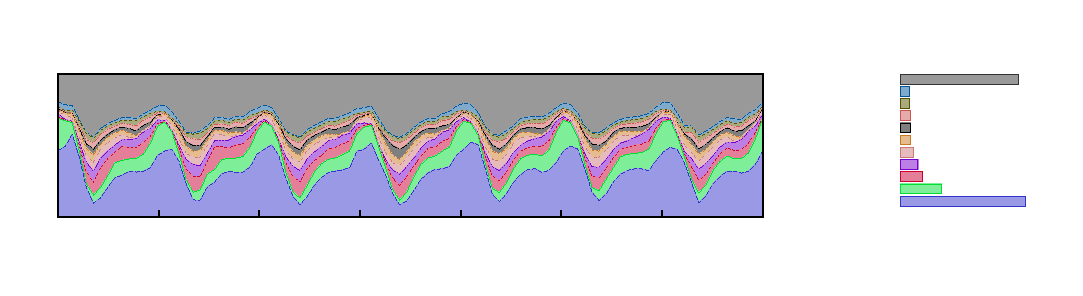
\includegraphics{img/day-und}}%
    \gplfronttext
  \end{picture}%
\endgroup


\noindent% GNUPLOT: LaTeX picture with Postscript
\begingroup
  \makeatletter
  \providecommand\color[2][]{%
    \GenericError{(gnuplot) \space\space\space\@spaces}{%
      Package color not loaded in conjunction with
      terminal option `colourtext'%
    }{See the gnuplot documentation for explanation.%
    }{Either use 'blacktext' in gnuplot or load the package
      color.sty in LaTeX.}%
    \renewcommand\color[2][]{}%
  }%
  \providecommand\includegraphics[2][]{%
    \GenericError{(gnuplot) \space\space\space\@spaces}{%
      Package graphicx or graphics not loaded%
    }{See the gnuplot documentation for explanation.%
    }{The gnuplot epslatex terminal needs graphicx.sty or graphics.sty.}%
    \renewcommand\includegraphics[2][]{}%
  }%
  \providecommand\rotatebox[2]{#2}%
  \@ifundefined{ifGPcolor}{%
    \newif\ifGPcolor
    \GPcolorfalse
  }{}%
  \@ifundefined{ifGPblacktext}{%
    \newif\ifGPblacktext
    \GPblacktexttrue
  }{}%
  % define a \g@addto@macro without @ in the name:
  \let\gplgaddtomacro\g@addto@macro
  % define empty templates for all commands taking text:
  \gdef\gplbacktext{}%
  \gdef\gplfronttext{}%
  \makeatother
  \ifGPblacktext
    % no textcolor at all
    \def\colorrgb#1{}%
    \def\colorgray#1{}%
  \else
    % gray or color?
    \ifGPcolor
      \def\colorrgb#1{\color[rgb]{#1}}%
      \def\colorgray#1{\color[gray]{#1}}%
      \expandafter\def\csname LTw\endcsname{\color{white}}%
      \expandafter\def\csname LTb\endcsname{\color{black}}%
      \expandafter\def\csname LTa\endcsname{\color{black}}%
      \expandafter\def\csname LT0\endcsname{\color[rgb]{1,0,0}}%
      \expandafter\def\csname LT1\endcsname{\color[rgb]{0,1,0}}%
      \expandafter\def\csname LT2\endcsname{\color[rgb]{0,0,1}}%
      \expandafter\def\csname LT3\endcsname{\color[rgb]{1,0,1}}%
      \expandafter\def\csname LT4\endcsname{\color[rgb]{0,1,1}}%
      \expandafter\def\csname LT5\endcsname{\color[rgb]{1,1,0}}%
      \expandafter\def\csname LT6\endcsname{\color[rgb]{0,0,0}}%
      \expandafter\def\csname LT7\endcsname{\color[rgb]{1,0.3,0}}%
      \expandafter\def\csname LT8\endcsname{\color[rgb]{0.5,0.5,0.5}}%
    \else
      % gray
      \def\colorrgb#1{\color{black}}%
      \def\colorgray#1{\color[gray]{#1}}%
      \expandafter\def\csname LTw\endcsname{\color{white}}%
      \expandafter\def\csname LTb\endcsname{\color{black}}%
      \expandafter\def\csname LTa\endcsname{\color{black}}%
      \expandafter\def\csname LT0\endcsname{\color{black}}%
      \expandafter\def\csname LT1\endcsname{\color{black}}%
      \expandafter\def\csname LT2\endcsname{\color{black}}%
      \expandafter\def\csname LT3\endcsname{\color{black}}%
      \expandafter\def\csname LT4\endcsname{\color{black}}%
      \expandafter\def\csname LT5\endcsname{\color{black}}%
      \expandafter\def\csname LT6\endcsname{\color{black}}%
      \expandafter\def\csname LT7\endcsname{\color{black}}%
      \expandafter\def\csname LT8\endcsname{\color{black}}%
    \fi
  \fi
  \setlength{\unitlength}{0.0500bp}%
  \begin{picture}(10080.00,2520.00)%
    \gplgaddtomacro\gplbacktext{%
      \csname LTb\endcsname%
      \put(176,1281){\rotatebox{-270}{\makebox(0,0){\strut{}\scriptsize fraction of tweets}}}%
      \put(3779,154){\makebox(0,0){\strut{}\scriptsize day of week(UTC)}}%
      \put(3779,2189){\makebox(0,0){\strut{}Countries that Tweet in German}}%
    }%
    \gplgaddtomacro\gplfronttext{%
      \csname LTb\endcsname%
      \put(396,374){\makebox(0,0){\strut{}\scriptsize 0}}%
      \put(1363,374){\makebox(0,0){\strut{}\scriptsize 1}}%
      \put(2329,374){\makebox(0,0){\strut{}\scriptsize 2}}%
      \put(3296,374){\makebox(0,0){\strut{}\scriptsize 3}}%
      \put(4263,374){\makebox(0,0){\strut{}\scriptsize 4}}%
      \put(5230,374){\makebox(0,0){\strut{}\scriptsize 5}}%
      \put(6196,374){\makebox(0,0){\strut{}\scriptsize 6}}%
      \put(7163,374){\makebox(0,0){\strut{}\scriptsize 7}}%
    }%
    \gplgaddtomacro\gplbacktext{%
      \csname LTb\endcsname%
      \put(9083,154){\makebox(0,0){\strut{}~~}}%
      \put(9083,2189){\makebox(0,0){\strut{} }}%
    }%
    \gplgaddtomacro\gplfronttext{%
      \csname LTb\endcsname%
      \put(8352,751){\makebox(0,0)[r]{\strut{}\scriptsize~DE}}%
      \put(8352,868){\makebox(0,0)[r]{\strut{}\scriptsize~USA}}%
      \put(8352,985){\makebox(0,0)[r]{\strut{}\scriptsize~AT}}%
      \put(8352,1102){\makebox(0,0)[r]{\strut{}\scriptsize~Switzerland}}%
      \put(8352,1219){\makebox(0,0)[r]{\strut{}\scriptsize~DZ}}%
      \put(8352,1337){\makebox(0,0)[r]{\strut{}\scriptsize~Brazil}}%
      \put(8352,1454){\makebox(0,0)[r]{\strut{}\scriptsize~UK}}%
      \put(8352,1571){\makebox(0,0)[r]{\strut{}\scriptsize~Philippines}}%
      \put(8352,1688){\makebox(0,0)[r]{\strut{}\scriptsize~Spain}}%
      \put(8352,1805){\makebox(0,0)[r]{\strut{}\scriptsize~France}}%
      \put(8352,1922){\makebox(0,0)[r]{\strut{}\scriptsize~other}}%
    }%
    \gplbacktext
    \put(0,0){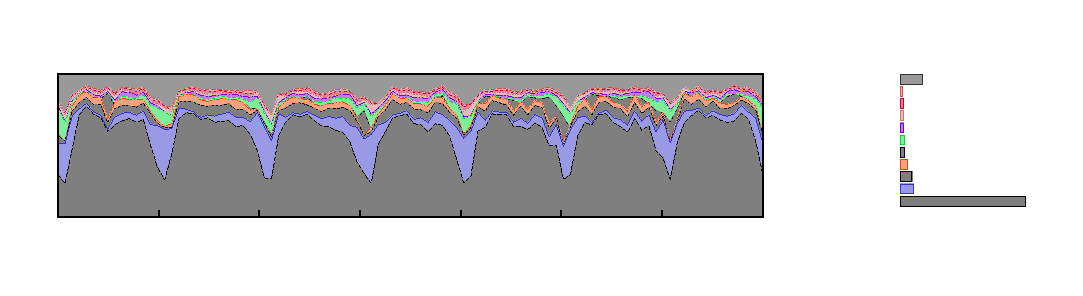
\includegraphics{img/day-de}}%
    \gplfronttext
  \end{picture}%
\endgroup


\noindent% GNUPLOT: LaTeX picture with Postscript
\begingroup
  \makeatletter
  \providecommand\color[2][]{%
    \GenericError{(gnuplot) \space\space\space\@spaces}{%
      Package color not loaded in conjunction with
      terminal option `colourtext'%
    }{See the gnuplot documentation for explanation.%
    }{Either use 'blacktext' in gnuplot or load the package
      color.sty in LaTeX.}%
    \renewcommand\color[2][]{}%
  }%
  \providecommand\includegraphics[2][]{%
    \GenericError{(gnuplot) \space\space\space\@spaces}{%
      Package graphicx or graphics not loaded%
    }{See the gnuplot documentation for explanation.%
    }{The gnuplot epslatex terminal needs graphicx.sty or graphics.sty.}%
    \renewcommand\includegraphics[2][]{}%
  }%
  \providecommand\rotatebox[2]{#2}%
  \@ifundefined{ifGPcolor}{%
    \newif\ifGPcolor
    \GPcolorfalse
  }{}%
  \@ifundefined{ifGPblacktext}{%
    \newif\ifGPblacktext
    \GPblacktexttrue
  }{}%
  % define a \g@addto@macro without @ in the name:
  \let\gplgaddtomacro\g@addto@macro
  % define empty templates for all commands taking text:
  \gdef\gplbacktext{}%
  \gdef\gplfronttext{}%
  \makeatother
  \ifGPblacktext
    % no textcolor at all
    \def\colorrgb#1{}%
    \def\colorgray#1{}%
  \else
    % gray or color?
    \ifGPcolor
      \def\colorrgb#1{\color[rgb]{#1}}%
      \def\colorgray#1{\color[gray]{#1}}%
      \expandafter\def\csname LTw\endcsname{\color{white}}%
      \expandafter\def\csname LTb\endcsname{\color{black}}%
      \expandafter\def\csname LTa\endcsname{\color{black}}%
      \expandafter\def\csname LT0\endcsname{\color[rgb]{1,0,0}}%
      \expandafter\def\csname LT1\endcsname{\color[rgb]{0,1,0}}%
      \expandafter\def\csname LT2\endcsname{\color[rgb]{0,0,1}}%
      \expandafter\def\csname LT3\endcsname{\color[rgb]{1,0,1}}%
      \expandafter\def\csname LT4\endcsname{\color[rgb]{0,1,1}}%
      \expandafter\def\csname LT5\endcsname{\color[rgb]{1,1,0}}%
      \expandafter\def\csname LT6\endcsname{\color[rgb]{0,0,0}}%
      \expandafter\def\csname LT7\endcsname{\color[rgb]{1,0.3,0}}%
      \expandafter\def\csname LT8\endcsname{\color[rgb]{0.5,0.5,0.5}}%
    \else
      % gray
      \def\colorrgb#1{\color{black}}%
      \def\colorgray#1{\color[gray]{#1}}%
      \expandafter\def\csname LTw\endcsname{\color{white}}%
      \expandafter\def\csname LTb\endcsname{\color{black}}%
      \expandafter\def\csname LTa\endcsname{\color{black}}%
      \expandafter\def\csname LT0\endcsname{\color{black}}%
      \expandafter\def\csname LT1\endcsname{\color{black}}%
      \expandafter\def\csname LT2\endcsname{\color{black}}%
      \expandafter\def\csname LT3\endcsname{\color{black}}%
      \expandafter\def\csname LT4\endcsname{\color{black}}%
      \expandafter\def\csname LT5\endcsname{\color{black}}%
      \expandafter\def\csname LT6\endcsname{\color{black}}%
      \expandafter\def\csname LT7\endcsname{\color{black}}%
      \expandafter\def\csname LT8\endcsname{\color{black}}%
    \fi
  \fi
  \setlength{\unitlength}{0.0500bp}%
  \begin{picture}(10080.00,2520.00)%
    \gplgaddtomacro\gplbacktext{%
      \csname LTb\endcsname%
      \put(176,1281){\rotatebox{-270}{\makebox(0,0){\strut{}\scriptsize fraction of tweets}}}%
      \put(3779,154){\makebox(0,0){\strut{}\scriptsize day of week(UTC)}}%
      \put(3779,2189){\makebox(0,0){\strut{}Countries that Tweet in Dutch}}%
    }%
    \gplgaddtomacro\gplfronttext{%
      \csname LTb\endcsname%
      \put(396,374){\makebox(0,0){\strut{}\scriptsize 0}}%
      \put(1363,374){\makebox(0,0){\strut{}\scriptsize 1}}%
      \put(2329,374){\makebox(0,0){\strut{}\scriptsize 2}}%
      \put(3296,374){\makebox(0,0){\strut{}\scriptsize 3}}%
      \put(4263,374){\makebox(0,0){\strut{}\scriptsize 4}}%
      \put(5230,374){\makebox(0,0){\strut{}\scriptsize 5}}%
      \put(6196,374){\makebox(0,0){\strut{}\scriptsize 6}}%
      \put(7163,374){\makebox(0,0){\strut{}\scriptsize 7}}%
    }%
    \gplgaddtomacro\gplbacktext{%
      \csname LTb\endcsname%
      \put(9083,154){\makebox(0,0){\strut{}~~}}%
      \put(9083,2189){\makebox(0,0){\strut{} }}%
    }%
    \gplgaddtomacro\gplfronttext{%
      \csname LTb\endcsname%
      \put(8352,751){\makebox(0,0)[r]{\strut{}\scriptsize~NL}}%
      \put(8352,868){\makebox(0,0)[r]{\strut{}\scriptsize~Belgium}}%
      \put(8352,985){\makebox(0,0)[r]{\strut{}\scriptsize~USA}}%
      \put(8352,1102){\makebox(0,0)[r]{\strut{}\scriptsize~Philippines}}%
      \put(8352,1219){\makebox(0,0)[r]{\strut{}\scriptsize~UK}}%
      \put(8352,1337){\makebox(0,0)[r]{\strut{}\scriptsize~South~Africa}}%
      \put(8352,1454){\makebox(0,0)[r]{\strut{}\scriptsize~Brazil}}%
      \put(8352,1571){\makebox(0,0)[r]{\strut{}\scriptsize~Spain}}%
      \put(8352,1688){\makebox(0,0)[r]{\strut{}\scriptsize~DE}}%
      \put(8352,1805){\makebox(0,0)[r]{\strut{}\scriptsize~France}}%
      \put(8352,1922){\makebox(0,0)[r]{\strut{}\scriptsize~other}}%
    }%
    \gplbacktext
    \put(0,0){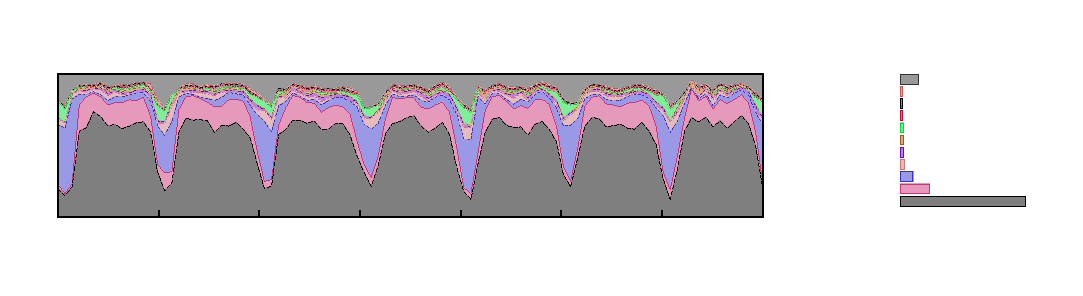
\includegraphics{img/day-nl}}%
    \gplfronttext
  \end{picture}%
\endgroup


\noindent% GNUPLOT: LaTeX picture with Postscript
\begingroup
  \makeatletter
  \providecommand\color[2][]{%
    \GenericError{(gnuplot) \space\space\space\@spaces}{%
      Package color not loaded in conjunction with
      terminal option `colourtext'%
    }{See the gnuplot documentation for explanation.%
    }{Either use 'blacktext' in gnuplot or load the package
      color.sty in LaTeX.}%
    \renewcommand\color[2][]{}%
  }%
  \providecommand\includegraphics[2][]{%
    \GenericError{(gnuplot) \space\space\space\@spaces}{%
      Package graphicx or graphics not loaded%
    }{See the gnuplot documentation for explanation.%
    }{The gnuplot epslatex terminal needs graphicx.sty or graphics.sty.}%
    \renewcommand\includegraphics[2][]{}%
  }%
  \providecommand\rotatebox[2]{#2}%
  \@ifundefined{ifGPcolor}{%
    \newif\ifGPcolor
    \GPcolorfalse
  }{}%
  \@ifundefined{ifGPblacktext}{%
    \newif\ifGPblacktext
    \GPblacktexttrue
  }{}%
  % define a \g@addto@macro without @ in the name:
  \let\gplgaddtomacro\g@addto@macro
  % define empty templates for all commands taking text:
  \gdef\gplbacktext{}%
  \gdef\gplfronttext{}%
  \makeatother
  \ifGPblacktext
    % no textcolor at all
    \def\colorrgb#1{}%
    \def\colorgray#1{}%
  \else
    % gray or color?
    \ifGPcolor
      \def\colorrgb#1{\color[rgb]{#1}}%
      \def\colorgray#1{\color[gray]{#1}}%
      \expandafter\def\csname LTw\endcsname{\color{white}}%
      \expandafter\def\csname LTb\endcsname{\color{black}}%
      \expandafter\def\csname LTa\endcsname{\color{black}}%
      \expandafter\def\csname LT0\endcsname{\color[rgb]{1,0,0}}%
      \expandafter\def\csname LT1\endcsname{\color[rgb]{0,1,0}}%
      \expandafter\def\csname LT2\endcsname{\color[rgb]{0,0,1}}%
      \expandafter\def\csname LT3\endcsname{\color[rgb]{1,0,1}}%
      \expandafter\def\csname LT4\endcsname{\color[rgb]{0,1,1}}%
      \expandafter\def\csname LT5\endcsname{\color[rgb]{1,1,0}}%
      \expandafter\def\csname LT6\endcsname{\color[rgb]{0,0,0}}%
      \expandafter\def\csname LT7\endcsname{\color[rgb]{1,0.3,0}}%
      \expandafter\def\csname LT8\endcsname{\color[rgb]{0.5,0.5,0.5}}%
    \else
      % gray
      \def\colorrgb#1{\color{black}}%
      \def\colorgray#1{\color[gray]{#1}}%
      \expandafter\def\csname LTw\endcsname{\color{white}}%
      \expandafter\def\csname LTb\endcsname{\color{black}}%
      \expandafter\def\csname LTa\endcsname{\color{black}}%
      \expandafter\def\csname LT0\endcsname{\color{black}}%
      \expandafter\def\csname LT1\endcsname{\color{black}}%
      \expandafter\def\csname LT2\endcsname{\color{black}}%
      \expandafter\def\csname LT3\endcsname{\color{black}}%
      \expandafter\def\csname LT4\endcsname{\color{black}}%
      \expandafter\def\csname LT5\endcsname{\color{black}}%
      \expandafter\def\csname LT6\endcsname{\color{black}}%
      \expandafter\def\csname LT7\endcsname{\color{black}}%
      \expandafter\def\csname LT8\endcsname{\color{black}}%
    \fi
  \fi
  \setlength{\unitlength}{0.0500bp}%
  \begin{picture}(10080.00,2520.00)%
    \gplgaddtomacro\gplbacktext{%
      \csname LTb\endcsname%
      \put(176,1281){\rotatebox{-270}{\makebox(0,0){\strut{}\scriptsize fraction of tweets}}}%
      \put(3779,154){\makebox(0,0){\strut{}\scriptsize day of week(UTC)}}%
      \put(3779,2189){\makebox(0,0){\strut{}Countries that Tweet in Czech}}%
    }%
    \gplgaddtomacro\gplfronttext{%
      \csname LTb\endcsname%
      \put(396,374){\makebox(0,0){\strut{}\scriptsize 0}}%
      \put(1363,374){\makebox(0,0){\strut{}\scriptsize 1}}%
      \put(2329,374){\makebox(0,0){\strut{}\scriptsize 2}}%
      \put(3296,374){\makebox(0,0){\strut{}\scriptsize 3}}%
      \put(4263,374){\makebox(0,0){\strut{}\scriptsize 4}}%
      \put(5230,374){\makebox(0,0){\strut{}\scriptsize 5}}%
      \put(6196,374){\makebox(0,0){\strut{}\scriptsize 6}}%
      \put(7163,374){\makebox(0,0){\strut{}\scriptsize 7}}%
    }%
    \gplgaddtomacro\gplbacktext{%
      \csname LTb\endcsname%
      \put(9083,154){\makebox(0,0){\strut{}~~}}%
      \put(9083,2189){\makebox(0,0){\strut{} }}%
    }%
    \gplgaddtomacro\gplfronttext{%
      \csname LTb\endcsname%
      \put(8352,751){\makebox(0,0)[r]{\strut{}\scriptsize~CZ}}%
      \put(8352,868){\makebox(0,0)[r]{\strut{}\scriptsize~Brazil}}%
      \put(8352,985){\makebox(0,0)[r]{\strut{}\scriptsize~USA}}%
      \put(8352,1102){\makebox(0,0)[r]{\strut{}\scriptsize~Spain}}%
      \put(8352,1219){\makebox(0,0)[r]{\strut{}\scriptsize~Philippines}}%
      \put(8352,1337){\makebox(0,0)[r]{\strut{}\scriptsize~Russia}}%
      \put(8352,1454){\makebox(0,0)[r]{\strut{}\scriptsize~UK}}%
      \put(8352,1571){\makebox(0,0)[r]{\strut{}\scriptsize~France}}%
      \put(8352,1688){\makebox(0,0)[r]{\strut{}\scriptsize~South~Africa}}%
      \put(8352,1805){\makebox(0,0)[r]{\strut{}\scriptsize~Italy}}%
      \put(8352,1922){\makebox(0,0)[r]{\strut{}\scriptsize~other}}%
    }%
    \gplbacktext
    \put(0,0){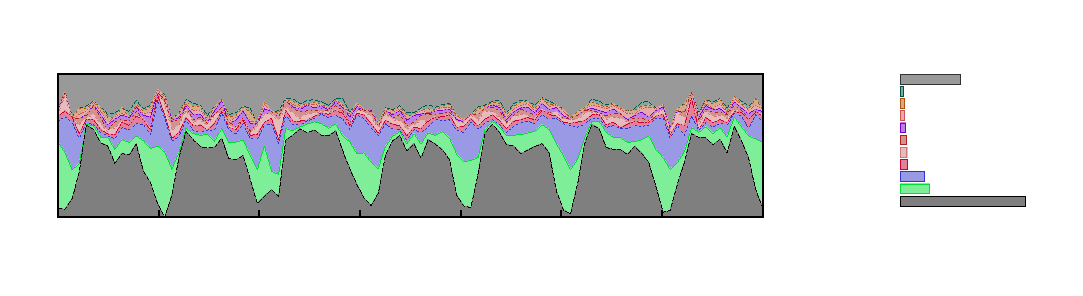
\includegraphics{img/day-cs}}%
    \gplfronttext
  \end{picture}%
\endgroup


\noindent% GNUPLOT: LaTeX picture with Postscript
\begingroup
  \makeatletter
  \providecommand\color[2][]{%
    \GenericError{(gnuplot) \space\space\space\@spaces}{%
      Package color not loaded in conjunction with
      terminal option `colourtext'%
    }{See the gnuplot documentation for explanation.%
    }{Either use 'blacktext' in gnuplot or load the package
      color.sty in LaTeX.}%
    \renewcommand\color[2][]{}%
  }%
  \providecommand\includegraphics[2][]{%
    \GenericError{(gnuplot) \space\space\space\@spaces}{%
      Package graphicx or graphics not loaded%
    }{See the gnuplot documentation for explanation.%
    }{The gnuplot epslatex terminal needs graphicx.sty or graphics.sty.}%
    \renewcommand\includegraphics[2][]{}%
  }%
  \providecommand\rotatebox[2]{#2}%
  \@ifundefined{ifGPcolor}{%
    \newif\ifGPcolor
    \GPcolorfalse
  }{}%
  \@ifundefined{ifGPblacktext}{%
    \newif\ifGPblacktext
    \GPblacktexttrue
  }{}%
  % define a \g@addto@macro without @ in the name:
  \let\gplgaddtomacro\g@addto@macro
  % define empty templates for all commands taking text:
  \gdef\gplbacktext{}%
  \gdef\gplfronttext{}%
  \makeatother
  \ifGPblacktext
    % no textcolor at all
    \def\colorrgb#1{}%
    \def\colorgray#1{}%
  \else
    % gray or color?
    \ifGPcolor
      \def\colorrgb#1{\color[rgb]{#1}}%
      \def\colorgray#1{\color[gray]{#1}}%
      \expandafter\def\csname LTw\endcsname{\color{white}}%
      \expandafter\def\csname LTb\endcsname{\color{black}}%
      \expandafter\def\csname LTa\endcsname{\color{black}}%
      \expandafter\def\csname LT0\endcsname{\color[rgb]{1,0,0}}%
      \expandafter\def\csname LT1\endcsname{\color[rgb]{0,1,0}}%
      \expandafter\def\csname LT2\endcsname{\color[rgb]{0,0,1}}%
      \expandafter\def\csname LT3\endcsname{\color[rgb]{1,0,1}}%
      \expandafter\def\csname LT4\endcsname{\color[rgb]{0,1,1}}%
      \expandafter\def\csname LT5\endcsname{\color[rgb]{1,1,0}}%
      \expandafter\def\csname LT6\endcsname{\color[rgb]{0,0,0}}%
      \expandafter\def\csname LT7\endcsname{\color[rgb]{1,0.3,0}}%
      \expandafter\def\csname LT8\endcsname{\color[rgb]{0.5,0.5,0.5}}%
    \else
      % gray
      \def\colorrgb#1{\color{black}}%
      \def\colorgray#1{\color[gray]{#1}}%
      \expandafter\def\csname LTw\endcsname{\color{white}}%
      \expandafter\def\csname LTb\endcsname{\color{black}}%
      \expandafter\def\csname LTa\endcsname{\color{black}}%
      \expandafter\def\csname LT0\endcsname{\color{black}}%
      \expandafter\def\csname LT1\endcsname{\color{black}}%
      \expandafter\def\csname LT2\endcsname{\color{black}}%
      \expandafter\def\csname LT3\endcsname{\color{black}}%
      \expandafter\def\csname LT4\endcsname{\color{black}}%
      \expandafter\def\csname LT5\endcsname{\color{black}}%
      \expandafter\def\csname LT6\endcsname{\color{black}}%
      \expandafter\def\csname LT7\endcsname{\color{black}}%
      \expandafter\def\csname LT8\endcsname{\color{black}}%
    \fi
  \fi
  \setlength{\unitlength}{0.0500bp}%
  \begin{picture}(10080.00,2520.00)%
    \gplgaddtomacro\gplbacktext{%
      \csname LTb\endcsname%
      \put(176,1281){\rotatebox{-270}{\makebox(0,0){\strut{}\scriptsize fraction of tweets}}}%
      \put(3779,154){\makebox(0,0){\strut{}\scriptsize day of week(UTC)}}%
      \put(3779,2189){\makebox(0,0){\strut{}Countries that Tweet in Danish}}%
    }%
    \gplgaddtomacro\gplfronttext{%
      \csname LTb\endcsname%
      \put(396,374){\makebox(0,0){\strut{}\scriptsize 0}}%
      \put(1363,374){\makebox(0,0){\strut{}\scriptsize 1}}%
      \put(2329,374){\makebox(0,0){\strut{}\scriptsize 2}}%
      \put(3296,374){\makebox(0,0){\strut{}\scriptsize 3}}%
      \put(4263,374){\makebox(0,0){\strut{}\scriptsize 4}}%
      \put(5230,374){\makebox(0,0){\strut{}\scriptsize 5}}%
      \put(6196,374){\makebox(0,0){\strut{}\scriptsize 6}}%
      \put(7163,374){\makebox(0,0){\strut{}\scriptsize 7}}%
    }%
    \gplgaddtomacro\gplbacktext{%
      \csname LTb\endcsname%
      \put(9083,154){\makebox(0,0){\strut{}~~}}%
      \put(9083,2189){\makebox(0,0){\strut{} }}%
    }%
    \gplgaddtomacro\gplfronttext{%
      \csname LTb\endcsname%
      \put(8352,751){\makebox(0,0)[r]{\strut{}\scriptsize~DK}}%
      \put(8352,868){\makebox(0,0)[r]{\strut{}\scriptsize~USA}}%
      \put(8352,985){\makebox(0,0)[r]{\strut{}\scriptsize~Brazil}}%
      \put(8352,1102){\makebox(0,0)[r]{\strut{}\scriptsize~NO}}%
      \put(8352,1219){\makebox(0,0)[r]{\strut{}\scriptsize~Philippines}}%
      \put(8352,1337){\makebox(0,0)[r]{\strut{}\scriptsize~UK}}%
      \put(8352,1454){\makebox(0,0)[r]{\strut{}\scriptsize~Indonesia}}%
      \put(8352,1571){\makebox(0,0)[r]{\strut{}\scriptsize~Malasia}}%
      \put(8352,1688){\makebox(0,0)[r]{\strut{}\scriptsize~SE}}%
      \put(8352,1805){\makebox(0,0)[r]{\strut{}\scriptsize~TR}}%
      \put(8352,1922){\makebox(0,0)[r]{\strut{}\scriptsize~other}}%
    }%
    \gplbacktext
    \put(0,0){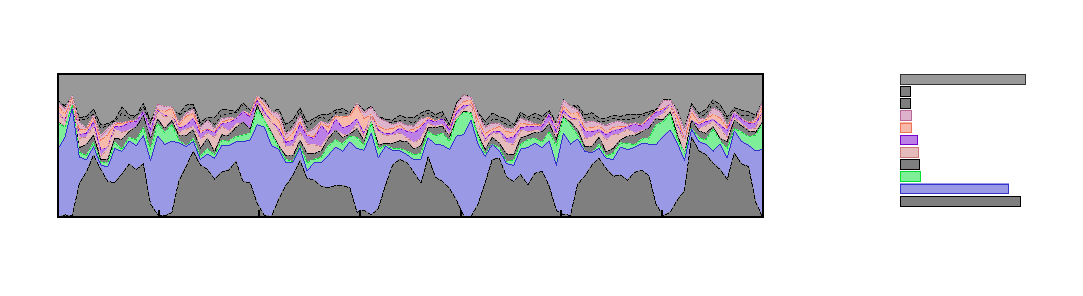
\includegraphics{img/day-da}}%
    \gplfronttext
  \end{picture}%
\endgroup


\noindent% GNUPLOT: LaTeX picture with Postscript
\begingroup
  \makeatletter
  \providecommand\color[2][]{%
    \GenericError{(gnuplot) \space\space\space\@spaces}{%
      Package color not loaded in conjunction with
      terminal option `colourtext'%
    }{See the gnuplot documentation for explanation.%
    }{Either use 'blacktext' in gnuplot or load the package
      color.sty in LaTeX.}%
    \renewcommand\color[2][]{}%
  }%
  \providecommand\includegraphics[2][]{%
    \GenericError{(gnuplot) \space\space\space\@spaces}{%
      Package graphicx or graphics not loaded%
    }{See the gnuplot documentation for explanation.%
    }{The gnuplot epslatex terminal needs graphicx.sty or graphics.sty.}%
    \renewcommand\includegraphics[2][]{}%
  }%
  \providecommand\rotatebox[2]{#2}%
  \@ifundefined{ifGPcolor}{%
    \newif\ifGPcolor
    \GPcolorfalse
  }{}%
  \@ifundefined{ifGPblacktext}{%
    \newif\ifGPblacktext
    \GPblacktexttrue
  }{}%
  % define a \g@addto@macro without @ in the name:
  \let\gplgaddtomacro\g@addto@macro
  % define empty templates for all commands taking text:
  \gdef\gplbacktext{}%
  \gdef\gplfronttext{}%
  \makeatother
  \ifGPblacktext
    % no textcolor at all
    \def\colorrgb#1{}%
    \def\colorgray#1{}%
  \else
    % gray or color?
    \ifGPcolor
      \def\colorrgb#1{\color[rgb]{#1}}%
      \def\colorgray#1{\color[gray]{#1}}%
      \expandafter\def\csname LTw\endcsname{\color{white}}%
      \expandafter\def\csname LTb\endcsname{\color{black}}%
      \expandafter\def\csname LTa\endcsname{\color{black}}%
      \expandafter\def\csname LT0\endcsname{\color[rgb]{1,0,0}}%
      \expandafter\def\csname LT1\endcsname{\color[rgb]{0,1,0}}%
      \expandafter\def\csname LT2\endcsname{\color[rgb]{0,0,1}}%
      \expandafter\def\csname LT3\endcsname{\color[rgb]{1,0,1}}%
      \expandafter\def\csname LT4\endcsname{\color[rgb]{0,1,1}}%
      \expandafter\def\csname LT5\endcsname{\color[rgb]{1,1,0}}%
      \expandafter\def\csname LT6\endcsname{\color[rgb]{0,0,0}}%
      \expandafter\def\csname LT7\endcsname{\color[rgb]{1,0.3,0}}%
      \expandafter\def\csname LT8\endcsname{\color[rgb]{0.5,0.5,0.5}}%
    \else
      % gray
      \def\colorrgb#1{\color{black}}%
      \def\colorgray#1{\color[gray]{#1}}%
      \expandafter\def\csname LTw\endcsname{\color{white}}%
      \expandafter\def\csname LTb\endcsname{\color{black}}%
      \expandafter\def\csname LTa\endcsname{\color{black}}%
      \expandafter\def\csname LT0\endcsname{\color{black}}%
      \expandafter\def\csname LT1\endcsname{\color{black}}%
      \expandafter\def\csname LT2\endcsname{\color{black}}%
      \expandafter\def\csname LT3\endcsname{\color{black}}%
      \expandafter\def\csname LT4\endcsname{\color{black}}%
      \expandafter\def\csname LT5\endcsname{\color{black}}%
      \expandafter\def\csname LT6\endcsname{\color{black}}%
      \expandafter\def\csname LT7\endcsname{\color{black}}%
      \expandafter\def\csname LT8\endcsname{\color{black}}%
    \fi
  \fi
  \setlength{\unitlength}{0.0500bp}%
  \begin{picture}(10080.00,2520.00)%
    \gplgaddtomacro\gplbacktext{%
      \csname LTb\endcsname%
      \put(176,1281){\rotatebox{-270}{\makebox(0,0){\strut{}\scriptsize fraction of tweets}}}%
      \put(3779,154){\makebox(0,0){\strut{}\scriptsize day of week(UTC)}}%
      \put(3779,2189){\makebox(0,0){\strut{}Countries that Tweet in Greek}}%
    }%
    \gplgaddtomacro\gplfronttext{%
      \csname LTb\endcsname%
      \put(396,374){\makebox(0,0){\strut{}\scriptsize 0}}%
      \put(1363,374){\makebox(0,0){\strut{}\scriptsize 1}}%
      \put(2329,374){\makebox(0,0){\strut{}\scriptsize 2}}%
      \put(3296,374){\makebox(0,0){\strut{}\scriptsize 3}}%
      \put(4263,374){\makebox(0,0){\strut{}\scriptsize 4}}%
      \put(5230,374){\makebox(0,0){\strut{}\scriptsize 5}}%
      \put(6196,374){\makebox(0,0){\strut{}\scriptsize 6}}%
      \put(7163,374){\makebox(0,0){\strut{}\scriptsize 7}}%
    }%
    \gplgaddtomacro\gplbacktext{%
      \csname LTb\endcsname%
      \put(9083,154){\makebox(0,0){\strut{}~~}}%
      \put(9083,2189){\makebox(0,0){\strut{} }}%
    }%
    \gplgaddtomacro\gplfronttext{%
      \csname LTb\endcsname%
      \put(8352,751){\makebox(0,0)[r]{\strut{}\scriptsize~GR}}%
      \put(8352,868){\makebox(0,0)[r]{\strut{}\scriptsize~CY}}%
      \put(8352,985){\makebox(0,0)[r]{\strut{}\scriptsize~France}}%
      \put(8352,1102){\makebox(0,0)[r]{\strut{}\scriptsize~UK}}%
      \put(8352,1219){\makebox(0,0)[r]{\strut{}\scriptsize~DE}}%
      \put(8352,1337){\makebox(0,0)[r]{\strut{}\scriptsize~USA}}%
      \put(8352,1454){\makebox(0,0)[r]{\strut{}\scriptsize~CZ}}%
      \put(8352,1571){\makebox(0,0)[r]{\strut{}\scriptsize~Italy}}%
      \put(8352,1688){\makebox(0,0)[r]{\strut{}\scriptsize~Belgium}}%
      \put(8352,1805){\makebox(0,0)[r]{\strut{}\scriptsize~Japan}}%
      \put(8352,1922){\makebox(0,0)[r]{\strut{}\scriptsize~other}}%
    }%
    \gplbacktext
    \put(0,0){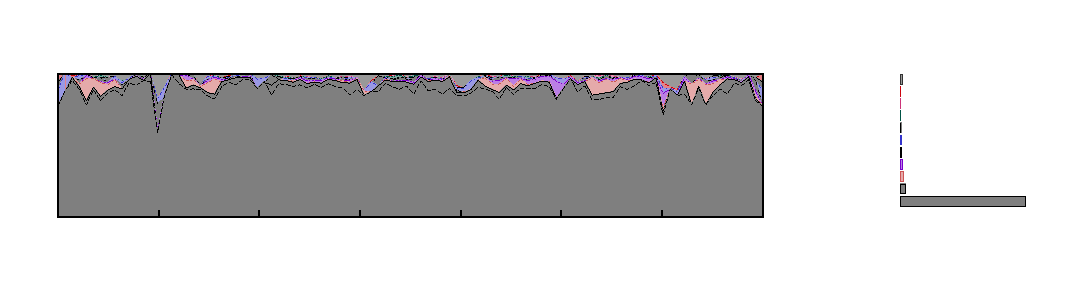
\includegraphics{img/day-el}}%
    \gplfronttext
  \end{picture}%
\endgroup


\noindent% GNUPLOT: LaTeX picture with Postscript
\begingroup
  \makeatletter
  \providecommand\color[2][]{%
    \GenericError{(gnuplot) \space\space\space\@spaces}{%
      Package color not loaded in conjunction with
      terminal option `colourtext'%
    }{See the gnuplot documentation for explanation.%
    }{Either use 'blacktext' in gnuplot or load the package
      color.sty in LaTeX.}%
    \renewcommand\color[2][]{}%
  }%
  \providecommand\includegraphics[2][]{%
    \GenericError{(gnuplot) \space\space\space\@spaces}{%
      Package graphicx or graphics not loaded%
    }{See the gnuplot documentation for explanation.%
    }{The gnuplot epslatex terminal needs graphicx.sty or graphics.sty.}%
    \renewcommand\includegraphics[2][]{}%
  }%
  \providecommand\rotatebox[2]{#2}%
  \@ifundefined{ifGPcolor}{%
    \newif\ifGPcolor
    \GPcolorfalse
  }{}%
  \@ifundefined{ifGPblacktext}{%
    \newif\ifGPblacktext
    \GPblacktexttrue
  }{}%
  % define a \g@addto@macro without @ in the name:
  \let\gplgaddtomacro\g@addto@macro
  % define empty templates for all commands taking text:
  \gdef\gplbacktext{}%
  \gdef\gplfronttext{}%
  \makeatother
  \ifGPblacktext
    % no textcolor at all
    \def\colorrgb#1{}%
    \def\colorgray#1{}%
  \else
    % gray or color?
    \ifGPcolor
      \def\colorrgb#1{\color[rgb]{#1}}%
      \def\colorgray#1{\color[gray]{#1}}%
      \expandafter\def\csname LTw\endcsname{\color{white}}%
      \expandafter\def\csname LTb\endcsname{\color{black}}%
      \expandafter\def\csname LTa\endcsname{\color{black}}%
      \expandafter\def\csname LT0\endcsname{\color[rgb]{1,0,0}}%
      \expandafter\def\csname LT1\endcsname{\color[rgb]{0,1,0}}%
      \expandafter\def\csname LT2\endcsname{\color[rgb]{0,0,1}}%
      \expandafter\def\csname LT3\endcsname{\color[rgb]{1,0,1}}%
      \expandafter\def\csname LT4\endcsname{\color[rgb]{0,1,1}}%
      \expandafter\def\csname LT5\endcsname{\color[rgb]{1,1,0}}%
      \expandafter\def\csname LT6\endcsname{\color[rgb]{0,0,0}}%
      \expandafter\def\csname LT7\endcsname{\color[rgb]{1,0.3,0}}%
      \expandafter\def\csname LT8\endcsname{\color[rgb]{0.5,0.5,0.5}}%
    \else
      % gray
      \def\colorrgb#1{\color{black}}%
      \def\colorgray#1{\color[gray]{#1}}%
      \expandafter\def\csname LTw\endcsname{\color{white}}%
      \expandafter\def\csname LTb\endcsname{\color{black}}%
      \expandafter\def\csname LTa\endcsname{\color{black}}%
      \expandafter\def\csname LT0\endcsname{\color{black}}%
      \expandafter\def\csname LT1\endcsname{\color{black}}%
      \expandafter\def\csname LT2\endcsname{\color{black}}%
      \expandafter\def\csname LT3\endcsname{\color{black}}%
      \expandafter\def\csname LT4\endcsname{\color{black}}%
      \expandafter\def\csname LT5\endcsname{\color{black}}%
      \expandafter\def\csname LT6\endcsname{\color{black}}%
      \expandafter\def\csname LT7\endcsname{\color{black}}%
      \expandafter\def\csname LT8\endcsname{\color{black}}%
    \fi
  \fi
  \setlength{\unitlength}{0.0500bp}%
  \begin{picture}(10080.00,2520.00)%
    \gplgaddtomacro\gplbacktext{%
      \csname LTb\endcsname%
      \put(176,1281){\rotatebox{-270}{\makebox(0,0){\strut{}\scriptsize fraction of tweets}}}%
      \put(3779,154){\makebox(0,0){\strut{}\scriptsize day of week(UTC)}}%
      \put(3779,2189){\makebox(0,0){\strut{}Countries that Tweet in Polish}}%
    }%
    \gplgaddtomacro\gplfronttext{%
      \csname LTb\endcsname%
      \put(396,374){\makebox(0,0){\strut{}\scriptsize 0}}%
      \put(1363,374){\makebox(0,0){\strut{}\scriptsize 1}}%
      \put(2329,374){\makebox(0,0){\strut{}\scriptsize 2}}%
      \put(3296,374){\makebox(0,0){\strut{}\scriptsize 3}}%
      \put(4263,374){\makebox(0,0){\strut{}\scriptsize 4}}%
      \put(5230,374){\makebox(0,0){\strut{}\scriptsize 5}}%
      \put(6196,374){\makebox(0,0){\strut{}\scriptsize 6}}%
      \put(7163,374){\makebox(0,0){\strut{}\scriptsize 7}}%
    }%
    \gplgaddtomacro\gplbacktext{%
      \csname LTb\endcsname%
      \put(9083,154){\makebox(0,0){\strut{}~~}}%
      \put(9083,2189){\makebox(0,0){\strut{} }}%
    }%
    \gplgaddtomacro\gplfronttext{%
      \csname LTb\endcsname%
      \put(8352,751){\makebox(0,0)[r]{\strut{}\scriptsize~PL}}%
      \put(8352,868){\makebox(0,0)[r]{\strut{}\scriptsize~USA}}%
      \put(8352,985){\makebox(0,0)[r]{\strut{}\scriptsize~UK}}%
      \put(8352,1102){\makebox(0,0)[r]{\strut{}\scriptsize~Philippines}}%
      \put(8352,1219){\makebox(0,0)[r]{\strut{}\scriptsize~Brazil}}%
      \put(8352,1337){\makebox(0,0)[r]{\strut{}\scriptsize~Japan}}%
      \put(8352,1454){\makebox(0,0)[r]{\strut{}\scriptsize~South~Africa}}%
      \put(8352,1571){\makebox(0,0)[r]{\strut{}\scriptsize~Nigeria}}%
      \put(8352,1688){\makebox(0,0)[r]{\strut{}\scriptsize~DE}}%
      \put(8352,1805){\makebox(0,0)[r]{\strut{}\scriptsize~NO}}%
      \put(8352,1922){\makebox(0,0)[r]{\strut{}\scriptsize~other}}%
    }%
    \gplbacktext
    \put(0,0){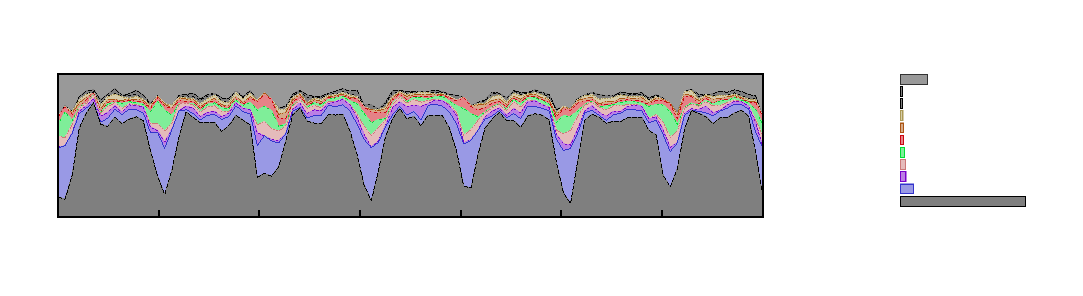
\includegraphics{img/day-pl}}%
    \gplfronttext
  \end{picture}%
\endgroup


\noindent% GNUPLOT: LaTeX picture with Postscript
\begingroup
  \makeatletter
  \providecommand\color[2][]{%
    \GenericError{(gnuplot) \space\space\space\@spaces}{%
      Package color not loaded in conjunction with
      terminal option `colourtext'%
    }{See the gnuplot documentation for explanation.%
    }{Either use 'blacktext' in gnuplot or load the package
      color.sty in LaTeX.}%
    \renewcommand\color[2][]{}%
  }%
  \providecommand\includegraphics[2][]{%
    \GenericError{(gnuplot) \space\space\space\@spaces}{%
      Package graphicx or graphics not loaded%
    }{See the gnuplot documentation for explanation.%
    }{The gnuplot epslatex terminal needs graphicx.sty or graphics.sty.}%
    \renewcommand\includegraphics[2][]{}%
  }%
  \providecommand\rotatebox[2]{#2}%
  \@ifundefined{ifGPcolor}{%
    \newif\ifGPcolor
    \GPcolorfalse
  }{}%
  \@ifundefined{ifGPblacktext}{%
    \newif\ifGPblacktext
    \GPblacktexttrue
  }{}%
  % define a \g@addto@macro without @ in the name:
  \let\gplgaddtomacro\g@addto@macro
  % define empty templates for all commands taking text:
  \gdef\gplbacktext{}%
  \gdef\gplfronttext{}%
  \makeatother
  \ifGPblacktext
    % no textcolor at all
    \def\colorrgb#1{}%
    \def\colorgray#1{}%
  \else
    % gray or color?
    \ifGPcolor
      \def\colorrgb#1{\color[rgb]{#1}}%
      \def\colorgray#1{\color[gray]{#1}}%
      \expandafter\def\csname LTw\endcsname{\color{white}}%
      \expandafter\def\csname LTb\endcsname{\color{black}}%
      \expandafter\def\csname LTa\endcsname{\color{black}}%
      \expandafter\def\csname LT0\endcsname{\color[rgb]{1,0,0}}%
      \expandafter\def\csname LT1\endcsname{\color[rgb]{0,1,0}}%
      \expandafter\def\csname LT2\endcsname{\color[rgb]{0,0,1}}%
      \expandafter\def\csname LT3\endcsname{\color[rgb]{1,0,1}}%
      \expandafter\def\csname LT4\endcsname{\color[rgb]{0,1,1}}%
      \expandafter\def\csname LT5\endcsname{\color[rgb]{1,1,0}}%
      \expandafter\def\csname LT6\endcsname{\color[rgb]{0,0,0}}%
      \expandafter\def\csname LT7\endcsname{\color[rgb]{1,0.3,0}}%
      \expandafter\def\csname LT8\endcsname{\color[rgb]{0.5,0.5,0.5}}%
    \else
      % gray
      \def\colorrgb#1{\color{black}}%
      \def\colorgray#1{\color[gray]{#1}}%
      \expandafter\def\csname LTw\endcsname{\color{white}}%
      \expandafter\def\csname LTb\endcsname{\color{black}}%
      \expandafter\def\csname LTa\endcsname{\color{black}}%
      \expandafter\def\csname LT0\endcsname{\color{black}}%
      \expandafter\def\csname LT1\endcsname{\color{black}}%
      \expandafter\def\csname LT2\endcsname{\color{black}}%
      \expandafter\def\csname LT3\endcsname{\color{black}}%
      \expandafter\def\csname LT4\endcsname{\color{black}}%
      \expandafter\def\csname LT5\endcsname{\color{black}}%
      \expandafter\def\csname LT6\endcsname{\color{black}}%
      \expandafter\def\csname LT7\endcsname{\color{black}}%
      \expandafter\def\csname LT8\endcsname{\color{black}}%
    \fi
  \fi
  \setlength{\unitlength}{0.0500bp}%
  \begin{picture}(10080.00,2520.00)%
    \gplgaddtomacro\gplbacktext{%
      \csname LTb\endcsname%
      \put(176,1281){\rotatebox{-270}{\makebox(0,0){\strut{}\scriptsize fraction of tweets}}}%
      \put(3779,154){\makebox(0,0){\strut{}\scriptsize day of week(UTC)}}%
      \put(3779,2189){\makebox(0,0){\strut{}Countries that Tweet in Russian}}%
    }%
    \gplgaddtomacro\gplfronttext{%
      \csname LTb\endcsname%
      \put(396,374){\makebox(0,0){\strut{}\scriptsize 0}}%
      \put(1363,374){\makebox(0,0){\strut{}\scriptsize 1}}%
      \put(2329,374){\makebox(0,0){\strut{}\scriptsize 2}}%
      \put(3296,374){\makebox(0,0){\strut{}\scriptsize 3}}%
      \put(4263,374){\makebox(0,0){\strut{}\scriptsize 4}}%
      \put(5230,374){\makebox(0,0){\strut{}\scriptsize 5}}%
      \put(6196,374){\makebox(0,0){\strut{}\scriptsize 6}}%
      \put(7163,374){\makebox(0,0){\strut{}\scriptsize 7}}%
    }%
    \gplgaddtomacro\gplbacktext{%
      \csname LTb\endcsname%
      \put(9083,154){\makebox(0,0){\strut{}~~}}%
      \put(9083,2189){\makebox(0,0){\strut{} }}%
    }%
    \gplgaddtomacro\gplfronttext{%
      \csname LTb\endcsname%
      \put(8352,751){\makebox(0,0)[r]{\strut{}\scriptsize~Russia}}%
      \put(8352,868){\makebox(0,0)[r]{\strut{}\scriptsize~UA}}%
      \put(8352,985){\makebox(0,0)[r]{\strut{}\scriptsize~BY}}%
      \put(8352,1102){\makebox(0,0)[r]{\strut{}\scriptsize~MN}}%
      \put(8352,1219){\makebox(0,0)[r]{\strut{}\scriptsize~KZ}}%
      \put(8352,1337){\makebox(0,0)[r]{\strut{}\scriptsize~USA}}%
      \put(8352,1454){\makebox(0,0)[r]{\strut{}\scriptsize~DE}}%
      \put(8352,1571){\makebox(0,0)[r]{\strut{}\scriptsize~PL}}%
      \put(8352,1688){\makebox(0,0)[r]{\strut{}\scriptsize~CZ}}%
      \put(8352,1805){\makebox(0,0)[r]{\strut{}\scriptsize~NL}}%
      \put(8352,1922){\makebox(0,0)[r]{\strut{}\scriptsize~other}}%
    }%
    \gplbacktext
    \put(0,0){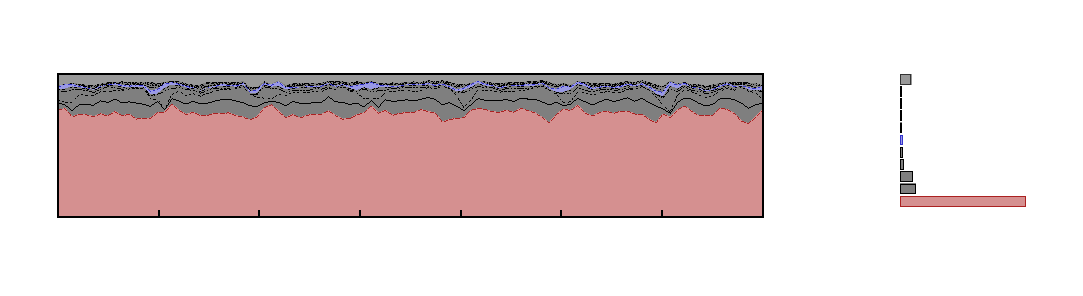
\includegraphics{img/day-ru}}%
    \gplfronttext
  \end{picture}%
\endgroup


\noindent% GNUPLOT: LaTeX picture with Postscript
\begingroup
  \makeatletter
  \providecommand\color[2][]{%
    \GenericError{(gnuplot) \space\space\space\@spaces}{%
      Package color not loaded in conjunction with
      terminal option `colourtext'%
    }{See the gnuplot documentation for explanation.%
    }{Either use 'blacktext' in gnuplot or load the package
      color.sty in LaTeX.}%
    \renewcommand\color[2][]{}%
  }%
  \providecommand\includegraphics[2][]{%
    \GenericError{(gnuplot) \space\space\space\@spaces}{%
      Package graphicx or graphics not loaded%
    }{See the gnuplot documentation for explanation.%
    }{The gnuplot epslatex terminal needs graphicx.sty or graphics.sty.}%
    \renewcommand\includegraphics[2][]{}%
  }%
  \providecommand\rotatebox[2]{#2}%
  \@ifundefined{ifGPcolor}{%
    \newif\ifGPcolor
    \GPcolorfalse
  }{}%
  \@ifundefined{ifGPblacktext}{%
    \newif\ifGPblacktext
    \GPblacktexttrue
  }{}%
  % define a \g@addto@macro without @ in the name:
  \let\gplgaddtomacro\g@addto@macro
  % define empty templates for all commands taking text:
  \gdef\gplbacktext{}%
  \gdef\gplfronttext{}%
  \makeatother
  \ifGPblacktext
    % no textcolor at all
    \def\colorrgb#1{}%
    \def\colorgray#1{}%
  \else
    % gray or color?
    \ifGPcolor
      \def\colorrgb#1{\color[rgb]{#1}}%
      \def\colorgray#1{\color[gray]{#1}}%
      \expandafter\def\csname LTw\endcsname{\color{white}}%
      \expandafter\def\csname LTb\endcsname{\color{black}}%
      \expandafter\def\csname LTa\endcsname{\color{black}}%
      \expandafter\def\csname LT0\endcsname{\color[rgb]{1,0,0}}%
      \expandafter\def\csname LT1\endcsname{\color[rgb]{0,1,0}}%
      \expandafter\def\csname LT2\endcsname{\color[rgb]{0,0,1}}%
      \expandafter\def\csname LT3\endcsname{\color[rgb]{1,0,1}}%
      \expandafter\def\csname LT4\endcsname{\color[rgb]{0,1,1}}%
      \expandafter\def\csname LT5\endcsname{\color[rgb]{1,1,0}}%
      \expandafter\def\csname LT6\endcsname{\color[rgb]{0,0,0}}%
      \expandafter\def\csname LT7\endcsname{\color[rgb]{1,0.3,0}}%
      \expandafter\def\csname LT8\endcsname{\color[rgb]{0.5,0.5,0.5}}%
    \else
      % gray
      \def\colorrgb#1{\color{black}}%
      \def\colorgray#1{\color[gray]{#1}}%
      \expandafter\def\csname LTw\endcsname{\color{white}}%
      \expandafter\def\csname LTb\endcsname{\color{black}}%
      \expandafter\def\csname LTa\endcsname{\color{black}}%
      \expandafter\def\csname LT0\endcsname{\color{black}}%
      \expandafter\def\csname LT1\endcsname{\color{black}}%
      \expandafter\def\csname LT2\endcsname{\color{black}}%
      \expandafter\def\csname LT3\endcsname{\color{black}}%
      \expandafter\def\csname LT4\endcsname{\color{black}}%
      \expandafter\def\csname LT5\endcsname{\color{black}}%
      \expandafter\def\csname LT6\endcsname{\color{black}}%
      \expandafter\def\csname LT7\endcsname{\color{black}}%
      \expandafter\def\csname LT8\endcsname{\color{black}}%
    \fi
  \fi
  \setlength{\unitlength}{0.0500bp}%
  \begin{picture}(10080.00,2520.00)%
    \gplgaddtomacro\gplbacktext{%
      \csname LTb\endcsname%
      \put(176,1281){\rotatebox{-270}{\makebox(0,0){\strut{}\scriptsize fraction of tweets}}}%
      \put(3779,154){\makebox(0,0){\strut{}\scriptsize day of week(UTC)}}%
      \put(3779,2189){\makebox(0,0){\strut{}Countries that Tweet in Vietnamese}}%
    }%
    \gplgaddtomacro\gplfronttext{%
      \csname LTb\endcsname%
      \put(396,374){\makebox(0,0){\strut{}\scriptsize 0}}%
      \put(1363,374){\makebox(0,0){\strut{}\scriptsize 1}}%
      \put(2329,374){\makebox(0,0){\strut{}\scriptsize 2}}%
      \put(3296,374){\makebox(0,0){\strut{}\scriptsize 3}}%
      \put(4263,374){\makebox(0,0){\strut{}\scriptsize 4}}%
      \put(5230,374){\makebox(0,0){\strut{}\scriptsize 5}}%
      \put(6196,374){\makebox(0,0){\strut{}\scriptsize 6}}%
      \put(7163,374){\makebox(0,0){\strut{}\scriptsize 7}}%
    }%
    \gplgaddtomacro\gplbacktext{%
      \csname LTb\endcsname%
      \put(9083,154){\makebox(0,0){\strut{}~~}}%
      \put(9083,2189){\makebox(0,0){\strut{} }}%
    }%
    \gplgaddtomacro\gplfronttext{%
      \csname LTb\endcsname%
      \put(8352,751){\makebox(0,0)[r]{\strut{}\scriptsize~VN}}%
      \put(8352,868){\makebox(0,0)[r]{\strut{}\scriptsize~Thailand}}%
      \put(8352,985){\makebox(0,0)[r]{\strut{}\scriptsize~Brazil}}%
      \put(8352,1102){\makebox(0,0)[r]{\strut{}\scriptsize~SN}}%
      \put(8352,1219){\makebox(0,0)[r]{\strut{}\scriptsize~South~Korea}}%
      \put(8352,1337){\makebox(0,0)[r]{\strut{}\scriptsize~USA}}%
      \put(8352,1454){\makebox(0,0)[r]{\strut{}\scriptsize~Philippines}}%
      \put(8352,1571){\makebox(0,0)[r]{\strut{}\scriptsize~Japan}}%
      \put(8352,1688){\makebox(0,0)[r]{\strut{}\scriptsize~India}}%
      \put(8352,1805){\makebox(0,0)[r]{\strut{}\scriptsize~France}}%
      \put(8352,1922){\makebox(0,0)[r]{\strut{}\scriptsize~other}}%
      \put(8484,484){\makebox(0,0){\strut{}\scriptsize 0}}%
      \put(8484,484){\makebox(0,0){\strut{}\scriptsize 1}}%
      \put(8484,484){\makebox(0,0){\strut{}\scriptsize 2}}%
      \put(8484,484){\makebox(0,0){\strut{}\scriptsize 3}}%
      \put(8485,484){\makebox(0,0){\strut{}\scriptsize 4}}%
      \put(8485,484){\makebox(0,0){\strut{}\scriptsize 5}}%
      \put(8485,484){\makebox(0,0){\strut{}\scriptsize 6}}%
      \put(8485,484){\makebox(0,0){\strut{}\scriptsize 7}}%
      \put(8485,484){\makebox(0,0){\strut{}\scriptsize 8}}%
      \put(8485,484){\makebox(0,0){\strut{}\scriptsize 9}}%
      \put(8485,484){\makebox(0,0){\strut{}\scriptsize 10}}%
      \put(8486,484){\makebox(0,0){\strut{}\scriptsize 11}}%
      \put(8486,484){\makebox(0,0){\strut{}\scriptsize 12}}%
      \put(8486,484){\makebox(0,0){\strut{}\scriptsize 13}}%
      \put(8486,484){\makebox(0,0){\strut{}\scriptsize 14}}%
      \put(8486,484){\makebox(0,0){\strut{}\scriptsize 15}}%
      \put(8486,484){\makebox(0,0){\strut{}\scriptsize 16}}%
      \put(8486,484){\makebox(0,0){\strut{}\scriptsize 17}}%
      \put(8487,484){\makebox(0,0){\strut{}\scriptsize 18}}%
      \put(8487,484){\makebox(0,0){\strut{}\scriptsize 19}}%
      \put(8487,484){\makebox(0,0){\strut{}\scriptsize 20}}%
      \put(8487,484){\makebox(0,0){\strut{}\scriptsize 21}}%
      \put(8487,484){\makebox(0,0){\strut{}\scriptsize 22}}%
      \put(8487,484){\makebox(0,0){\strut{}\scriptsize 23}}%
      \put(8487,484){\makebox(0,0){\strut{}\scriptsize 24}}%
      \put(8488,484){\makebox(0,0){\strut{}\scriptsize 25}}%
      \put(8488,484){\makebox(0,0){\strut{}\scriptsize 26}}%
      \put(8488,484){\makebox(0,0){\strut{}\scriptsize 27}}%
      \put(8488,484){\makebox(0,0){\strut{}\scriptsize 28}}%
      \put(8488,484){\makebox(0,0){\strut{}\scriptsize 29}}%
      \put(8488,484){\makebox(0,0){\strut{}\scriptsize 30}}%
      \put(8488,484){\makebox(0,0){\strut{}\scriptsize 31}}%
      \put(8489,484){\makebox(0,0){\strut{}\scriptsize 32}}%
      \put(8489,484){\makebox(0,0){\strut{}\scriptsize 33}}%
      \put(8489,484){\makebox(0,0){\strut{}\scriptsize 34}}%
      \put(8489,484){\makebox(0,0){\strut{}\scriptsize 35}}%
      \put(8489,484){\makebox(0,0){\strut{}\scriptsize 36}}%
      \put(8489,484){\makebox(0,0){\strut{}\scriptsize 37}}%
      \put(8489,484){\makebox(0,0){\strut{}\scriptsize 38}}%
      \put(8490,484){\makebox(0,0){\strut{}\scriptsize 39}}%
      \put(8490,484){\makebox(0,0){\strut{}\scriptsize 40}}%
      \put(8490,484){\makebox(0,0){\strut{}\scriptsize 41}}%
      \put(8490,484){\makebox(0,0){\strut{}\scriptsize 42}}%
      \put(8490,484){\makebox(0,0){\strut{}\scriptsize 43}}%
      \put(8490,484){\makebox(0,0){\strut{}\scriptsize 44}}%
      \put(8490,484){\makebox(0,0){\strut{}\scriptsize 45}}%
      \put(8491,484){\makebox(0,0){\strut{}\scriptsize 46}}%
      \put(8491,484){\makebox(0,0){\strut{}\scriptsize 47}}%
      \put(8491,484){\makebox(0,0){\strut{}\scriptsize 48}}%
      \put(8491,484){\makebox(0,0){\strut{}\scriptsize 49}}%
      \put(8491,484){\makebox(0,0){\strut{}\scriptsize 50}}%
      \put(8491,484){\makebox(0,0){\strut{}\scriptsize 51}}%
      \put(8491,484){\makebox(0,0){\strut{}\scriptsize 52}}%
      \put(8492,484){\makebox(0,0){\strut{}\scriptsize 53}}%
      \put(8492,484){\makebox(0,0){\strut{}\scriptsize 54}}%
      \put(8492,484){\makebox(0,0){\strut{}\scriptsize 55}}%
      \put(8492,484){\makebox(0,0){\strut{}\scriptsize 56}}%
      \put(8492,484){\makebox(0,0){\strut{}\scriptsize 57}}%
      \put(8492,484){\makebox(0,0){\strut{}\scriptsize 58}}%
      \put(8492,484){\makebox(0,0){\strut{}\scriptsize 59}}%
      \put(8493,484){\makebox(0,0){\strut{}\scriptsize 60}}%
      \put(8493,484){\makebox(0,0){\strut{}\scriptsize 61}}%
      \put(8493,484){\makebox(0,0){\strut{}\scriptsize 62}}%
      \put(8493,484){\makebox(0,0){\strut{}\scriptsize 63}}%
      \put(8493,484){\makebox(0,0){\strut{}\scriptsize 64}}%
      \put(8493,484){\makebox(0,0){\strut{}\scriptsize 65}}%
      \put(8493,484){\makebox(0,0){\strut{}\scriptsize 66}}%
      \put(8494,484){\makebox(0,0){\strut{}\scriptsize 67}}%
      \put(8494,484){\makebox(0,0){\strut{}\scriptsize 68}}%
      \put(8494,484){\makebox(0,0){\strut{}\scriptsize 69}}%
      \put(8494,484){\makebox(0,0){\strut{}\scriptsize 70}}%
      \put(8494,484){\makebox(0,0){\strut{}\scriptsize 71}}%
      \put(8494,484){\makebox(0,0){\strut{}\scriptsize 72}}%
      \put(8494,484){\makebox(0,0){\strut{}\scriptsize 73}}%
      \put(8495,484){\makebox(0,0){\strut{}\scriptsize 74}}%
      \put(8495,484){\makebox(0,0){\strut{}\scriptsize 75}}%
      \put(8495,484){\makebox(0,0){\strut{}\scriptsize 76}}%
      \put(8495,484){\makebox(0,0){\strut{}\scriptsize 77}}%
      \put(8495,484){\makebox(0,0){\strut{}\scriptsize 78}}%
      \put(8495,484){\makebox(0,0){\strut{}\scriptsize 79}}%
      \put(8495,484){\makebox(0,0){\strut{}\scriptsize 80}}%
      \put(8496,484){\makebox(0,0){\strut{}\scriptsize 81}}%
      \put(8496,484){\makebox(0,0){\strut{}\scriptsize 82}}%
      \put(8496,484){\makebox(0,0){\strut{}\scriptsize 83}}%
      \put(8496,484){\makebox(0,0){\strut{}\scriptsize 84}}%
      \put(8496,484){\makebox(0,0){\strut{}\scriptsize 85}}%
      \put(8496,484){\makebox(0,0){\strut{}\scriptsize 86}}%
      \put(8496,484){\makebox(0,0){\strut{}\scriptsize 87}}%
      \put(8497,484){\makebox(0,0){\strut{}\scriptsize 88}}%
      \put(8497,484){\makebox(0,0){\strut{}\scriptsize 89}}%
      \put(8497,484){\makebox(0,0){\strut{}\scriptsize 90}}%
      \put(8497,484){\makebox(0,0){\strut{}\scriptsize 91}}%
      \put(8497,484){\makebox(0,0){\strut{}\scriptsize 92}}%
      \put(8497,484){\makebox(0,0){\strut{}\scriptsize 93}}%
      \put(8497,484){\makebox(0,0){\strut{}\scriptsize 94}}%
      \put(8498,484){\makebox(0,0){\strut{}\scriptsize 95}}%
      \put(8498,484){\makebox(0,0){\strut{}\scriptsize 96}}%
      \put(8498,484){\makebox(0,0){\strut{}\scriptsize 97}}%
      \put(8498,484){\makebox(0,0){\strut{}\scriptsize 98}}%
      \put(8498,484){\makebox(0,0){\strut{}\scriptsize 99}}%
      \put(8498,484){\makebox(0,0){\strut{}\scriptsize 100}}%
      \put(8498,484){\makebox(0,0){\strut{}\scriptsize 101}}%
      \put(8499,484){\makebox(0,0){\strut{}\scriptsize 102}}%
      \put(8499,484){\makebox(0,0){\strut{}\scriptsize 103}}%
      \put(8499,484){\makebox(0,0){\strut{}\scriptsize 104}}%
      \put(8499,484){\makebox(0,0){\strut{}\scriptsize 105}}%
      \put(8499,484){\makebox(0,0){\strut{}\scriptsize 106}}%
      \put(8499,484){\makebox(0,0){\strut{}\scriptsize 107}}%
      \put(8499,484){\makebox(0,0){\strut{}\scriptsize 108}}%
      \put(8500,484){\makebox(0,0){\strut{}\scriptsize 109}}%
      \put(8500,484){\makebox(0,0){\strut{}\scriptsize 110}}%
      \put(8500,484){\makebox(0,0){\strut{}\scriptsize 111}}%
      \put(8500,484){\makebox(0,0){\strut{}\scriptsize 112}}%
      \put(8500,484){\makebox(0,0){\strut{}\scriptsize 113}}%
      \put(8500,484){\makebox(0,0){\strut{}\scriptsize 114}}%
      \put(8500,484){\makebox(0,0){\strut{}\scriptsize 115}}%
      \put(8501,484){\makebox(0,0){\strut{}\scriptsize 116}}%
      \put(8501,484){\makebox(0,0){\strut{}\scriptsize 117}}%
      \put(8501,484){\makebox(0,0){\strut{}\scriptsize 118}}%
      \put(8501,484){\makebox(0,0){\strut{}\scriptsize 119}}%
      \put(8501,484){\makebox(0,0){\strut{}\scriptsize 120}}%
      \put(8501,484){\makebox(0,0){\strut{}\scriptsize 121}}%
      \put(8501,484){\makebox(0,0){\strut{}\scriptsize 122}}%
      \put(8502,484){\makebox(0,0){\strut{}\scriptsize 123}}%
      \put(8502,484){\makebox(0,0){\strut{}\scriptsize 124}}%
      \put(8502,484){\makebox(0,0){\strut{}\scriptsize 125}}%
      \put(8502,484){\makebox(0,0){\strut{}\scriptsize 126}}%
      \put(8502,484){\makebox(0,0){\strut{}\scriptsize 127}}%
      \put(8502,484){\makebox(0,0){\strut{}\scriptsize 128}}%
      \put(8502,484){\makebox(0,0){\strut{}\scriptsize 129}}%
      \put(8503,484){\makebox(0,0){\strut{}\scriptsize 130}}%
      \put(8503,484){\makebox(0,0){\strut{}\scriptsize 131}}%
      \put(8503,484){\makebox(0,0){\strut{}\scriptsize 132}}%
      \put(8503,484){\makebox(0,0){\strut{}\scriptsize 133}}%
      \put(8503,484){\makebox(0,0){\strut{}\scriptsize 134}}%
      \put(8503,484){\makebox(0,0){\strut{}\scriptsize 135}}%
      \put(8503,484){\makebox(0,0){\strut{}\scriptsize 136}}%
      \put(8504,484){\makebox(0,0){\strut{}\scriptsize 137}}%
      \put(8504,484){\makebox(0,0){\strut{}\scriptsize 138}}%
      \put(8504,484){\makebox(0,0){\strut{}\scriptsize 139}}%
      \put(8504,484){\makebox(0,0){\strut{}\scriptsize 140}}%
      \put(8504,484){\makebox(0,0){\strut{}\scriptsize 141}}%
      \put(8504,484){\makebox(0,0){\strut{}\scriptsize 142}}%
      \put(8504,484){\makebox(0,0){\strut{}\scriptsize 143}}%
      \put(8505,484){\makebox(0,0){\strut{}\scriptsize 144}}%
      \put(8505,484){\makebox(0,0){\strut{}\scriptsize 145}}%
      \put(8505,484){\makebox(0,0){\strut{}\scriptsize 146}}%
      \put(8505,484){\makebox(0,0){\strut{}\scriptsize 147}}%
      \put(8505,484){\makebox(0,0){\strut{}\scriptsize 148}}%
      \put(8505,484){\makebox(0,0){\strut{}\scriptsize 149}}%
      \put(8505,484){\makebox(0,0){\strut{}\scriptsize 150}}%
      \put(8506,484){\makebox(0,0){\strut{}\scriptsize 151}}%
      \put(8506,484){\makebox(0,0){\strut{}\scriptsize 152}}%
      \put(8506,484){\makebox(0,0){\strut{}\scriptsize 153}}%
      \put(8506,484){\makebox(0,0){\strut{}\scriptsize 154}}%
      \put(8506,484){\makebox(0,0){\strut{}\scriptsize 155}}%
      \put(8506,484){\makebox(0,0){\strut{}\scriptsize 156}}%
      \put(8506,484){\makebox(0,0){\strut{}\scriptsize 157}}%
      \put(8507,484){\makebox(0,0){\strut{}\scriptsize 158}}%
      \put(8507,484){\makebox(0,0){\strut{}\scriptsize 159}}%
      \put(8507,484){\makebox(0,0){\strut{}\scriptsize 160}}%
      \put(8507,484){\makebox(0,0){\strut{}\scriptsize 161}}%
      \put(8507,484){\makebox(0,0){\strut{}\scriptsize 162}}%
      \put(8507,484){\makebox(0,0){\strut{}\scriptsize 163}}%
      \put(8507,484){\makebox(0,0){\strut{}\scriptsize 164}}%
      \put(8508,484){\makebox(0,0){\strut{}\scriptsize 165}}%
      \put(8508,484){\makebox(0,0){\strut{}\scriptsize 166}}%
      \put(8508,484){\makebox(0,0){\strut{}\scriptsize 167}}%
      \put(8508,484){\makebox(0,0){\strut{}\scriptsize 168}}%
      \put(8508,484){\makebox(0,0){\strut{}\scriptsize 169}}%
      \put(8508,484){\makebox(0,0){\strut{}\scriptsize 170}}%
      \put(8508,484){\makebox(0,0){\strut{}\scriptsize 171}}%
      \put(8509,484){\makebox(0,0){\strut{}\scriptsize 172}}%
      \put(8509,484){\makebox(0,0){\strut{}\scriptsize 173}}%
      \put(8509,484){\makebox(0,0){\strut{}\scriptsize 174}}%
      \put(8509,484){\makebox(0,0){\strut{}\scriptsize 175}}%
      \put(8509,484){\makebox(0,0){\strut{}\scriptsize 176}}%
      \put(8509,484){\makebox(0,0){\strut{}\scriptsize 177}}%
      \put(8509,484){\makebox(0,0){\strut{}\scriptsize 178}}%
      \put(8510,484){\makebox(0,0){\strut{}\scriptsize 179}}%
      \put(8510,484){\makebox(0,0){\strut{}\scriptsize 180}}%
      \put(8510,484){\makebox(0,0){\strut{}\scriptsize 181}}%
      \put(8510,484){\makebox(0,0){\strut{}\scriptsize 182}}%
      \put(8510,484){\makebox(0,0){\strut{}\scriptsize 183}}%
      \put(8510,484){\makebox(0,0){\strut{}\scriptsize 184}}%
      \put(8510,484){\makebox(0,0){\strut{}\scriptsize 185}}%
      \put(8511,484){\makebox(0,0){\strut{}\scriptsize 186}}%
      \put(8511,484){\makebox(0,0){\strut{}\scriptsize 187}}%
      \put(8511,484){\makebox(0,0){\strut{}\scriptsize 188}}%
      \put(8511,484){\makebox(0,0){\strut{}\scriptsize 189}}%
      \put(8511,484){\makebox(0,0){\strut{}\scriptsize 190}}%
      \put(8511,484){\makebox(0,0){\strut{}\scriptsize 191}}%
      \put(8511,484){\makebox(0,0){\strut{}\scriptsize 192}}%
      \put(8512,484){\makebox(0,0){\strut{}\scriptsize 193}}%
      \put(8512,484){\makebox(0,0){\strut{}\scriptsize 194}}%
      \put(8512,484){\makebox(0,0){\strut{}\scriptsize 195}}%
      \put(8512,484){\makebox(0,0){\strut{}\scriptsize 196}}%
      \put(8512,484){\makebox(0,0){\strut{}\scriptsize 197}}%
      \put(8512,484){\makebox(0,0){\strut{}\scriptsize 198}}%
      \put(8512,484){\makebox(0,0){\strut{}\scriptsize 199}}%
      \put(8513,484){\makebox(0,0){\strut{}\scriptsize 200}}%
      \put(8513,484){\makebox(0,0){\strut{}\scriptsize 201}}%
      \put(8513,484){\makebox(0,0){\strut{}\scriptsize 202}}%
      \put(8513,484){\makebox(0,0){\strut{}\scriptsize 203}}%
      \put(8513,484){\makebox(0,0){\strut{}\scriptsize 204}}%
      \put(8513,484){\makebox(0,0){\strut{}\scriptsize 205}}%
      \put(8513,484){\makebox(0,0){\strut{}\scriptsize 206}}%
      \put(8514,484){\makebox(0,0){\strut{}\scriptsize 207}}%
      \put(8514,484){\makebox(0,0){\strut{}\scriptsize 208}}%
      \put(8514,484){\makebox(0,0){\strut{}\scriptsize 209}}%
      \put(8514,484){\makebox(0,0){\strut{}\scriptsize 210}}%
      \put(8514,484){\makebox(0,0){\strut{}\scriptsize 211}}%
      \put(8514,484){\makebox(0,0){\strut{}\scriptsize 212}}%
      \put(8514,484){\makebox(0,0){\strut{}\scriptsize 213}}%
      \put(8515,484){\makebox(0,0){\strut{}\scriptsize 214}}%
      \put(8515,484){\makebox(0,0){\strut{}\scriptsize 215}}%
      \put(8515,484){\makebox(0,0){\strut{}\scriptsize 216}}%
      \put(8515,484){\makebox(0,0){\strut{}\scriptsize 217}}%
      \put(8515,484){\makebox(0,0){\strut{}\scriptsize 218}}%
      \put(8515,484){\makebox(0,0){\strut{}\scriptsize 219}}%
      \put(8515,484){\makebox(0,0){\strut{}\scriptsize 220}}%
      \put(8516,484){\makebox(0,0){\strut{}\scriptsize 221}}%
      \put(8516,484){\makebox(0,0){\strut{}\scriptsize 222}}%
      \put(8516,484){\makebox(0,0){\strut{}\scriptsize 223}}%
      \put(8516,484){\makebox(0,0){\strut{}\scriptsize 224}}%
      \put(8516,484){\makebox(0,0){\strut{}\scriptsize 225}}%
      \put(8516,484){\makebox(0,0){\strut{}\scriptsize 226}}%
      \put(8516,484){\makebox(0,0){\strut{}\scriptsize 227}}%
      \put(8517,484){\makebox(0,0){\strut{}\scriptsize 228}}%
      \put(8517,484){\makebox(0,0){\strut{}\scriptsize 229}}%
      \put(8517,484){\makebox(0,0){\strut{}\scriptsize 230}}%
      \put(8517,484){\makebox(0,0){\strut{}\scriptsize 231}}%
      \put(8517,484){\makebox(0,0){\strut{}\scriptsize 232}}%
      \put(8517,484){\makebox(0,0){\strut{}\scriptsize 233}}%
      \put(8517,484){\makebox(0,0){\strut{}\scriptsize 234}}%
      \put(8518,484){\makebox(0,0){\strut{}\scriptsize 235}}%
      \put(8518,484){\makebox(0,0){\strut{}\scriptsize 236}}%
      \put(8518,484){\makebox(0,0){\strut{}\scriptsize 237}}%
      \put(8518,484){\makebox(0,0){\strut{}\scriptsize 238}}%
      \put(8518,484){\makebox(0,0){\strut{}\scriptsize 239}}%
      \put(8518,484){\makebox(0,0){\strut{}\scriptsize 240}}%
      \put(8518,484){\makebox(0,0){\strut{}\scriptsize 241}}%
      \put(8519,484){\makebox(0,0){\strut{}\scriptsize 242}}%
      \put(8519,484){\makebox(0,0){\strut{}\scriptsize 243}}%
      \put(8519,484){\makebox(0,0){\strut{}\scriptsize 244}}%
      \put(8519,484){\makebox(0,0){\strut{}\scriptsize 245}}%
      \put(8519,484){\makebox(0,0){\strut{}\scriptsize 246}}%
      \put(8519,484){\makebox(0,0){\strut{}\scriptsize 247}}%
      \put(8519,484){\makebox(0,0){\strut{}\scriptsize 248}}%
      \put(8520,484){\makebox(0,0){\strut{}\scriptsize 249}}%
      \put(8520,484){\makebox(0,0){\strut{}\scriptsize 250}}%
      \put(8520,484){\makebox(0,0){\strut{}\scriptsize 251}}%
      \put(8520,484){\makebox(0,0){\strut{}\scriptsize 252}}%
      \put(8520,484){\makebox(0,0){\strut{}\scriptsize 253}}%
      \put(8520,484){\makebox(0,0){\strut{}\scriptsize 254}}%
      \put(8520,484){\makebox(0,0){\strut{}\scriptsize 255}}%
      \put(8521,484){\makebox(0,0){\strut{}\scriptsize 256}}%
      \put(8521,484){\makebox(0,0){\strut{}\scriptsize 257}}%
      \put(8521,484){\makebox(0,0){\strut{}\scriptsize 258}}%
      \put(8521,484){\makebox(0,0){\strut{}\scriptsize 259}}%
      \put(8521,484){\makebox(0,0){\strut{}\scriptsize 260}}%
      \put(8521,484){\makebox(0,0){\strut{}\scriptsize 261}}%
      \put(8521,484){\makebox(0,0){\strut{}\scriptsize 262}}%
      \put(8522,484){\makebox(0,0){\strut{}\scriptsize 263}}%
      \put(8522,484){\makebox(0,0){\strut{}\scriptsize 264}}%
      \put(8522,484){\makebox(0,0){\strut{}\scriptsize 265}}%
      \put(8522,484){\makebox(0,0){\strut{}\scriptsize 266}}%
      \put(8522,484){\makebox(0,0){\strut{}\scriptsize 267}}%
      \put(8522,484){\makebox(0,0){\strut{}\scriptsize 268}}%
      \put(8522,484){\makebox(0,0){\strut{}\scriptsize 269}}%
      \put(8523,484){\makebox(0,0){\strut{}\scriptsize 270}}%
      \put(8523,484){\makebox(0,0){\strut{}\scriptsize 271}}%
      \put(8523,484){\makebox(0,0){\strut{}\scriptsize 272}}%
      \put(8523,484){\makebox(0,0){\strut{}\scriptsize 273}}%
      \put(8523,484){\makebox(0,0){\strut{}\scriptsize 274}}%
      \put(8523,484){\makebox(0,0){\strut{}\scriptsize 275}}%
      \put(8523,484){\makebox(0,0){\strut{}\scriptsize 276}}%
      \put(8524,484){\makebox(0,0){\strut{}\scriptsize 277}}%
      \put(8524,484){\makebox(0,0){\strut{}\scriptsize 278}}%
      \put(8524,484){\makebox(0,0){\strut{}\scriptsize 279}}%
      \put(8524,484){\makebox(0,0){\strut{}\scriptsize 280}}%
      \put(8524,484){\makebox(0,0){\strut{}\scriptsize 281}}%
      \put(8524,484){\makebox(0,0){\strut{}\scriptsize 282}}%
      \put(8524,484){\makebox(0,0){\strut{}\scriptsize 283}}%
      \put(8525,484){\makebox(0,0){\strut{}\scriptsize 284}}%
      \put(8525,484){\makebox(0,0){\strut{}\scriptsize 285}}%
      \put(8525,484){\makebox(0,0){\strut{}\scriptsize 286}}%
      \put(8525,484){\makebox(0,0){\strut{}\scriptsize 287}}%
      \put(8525,484){\makebox(0,0){\strut{}\scriptsize 288}}%
      \put(8525,484){\makebox(0,0){\strut{}\scriptsize 289}}%
      \put(8525,484){\makebox(0,0){\strut{}\scriptsize 290}}%
      \put(8526,484){\makebox(0,0){\strut{}\scriptsize 291}}%
      \put(8526,484){\makebox(0,0){\strut{}\scriptsize 292}}%
      \put(8526,484){\makebox(0,0){\strut{}\scriptsize 293}}%
      \put(8526,484){\makebox(0,0){\strut{}\scriptsize 294}}%
      \put(8526,484){\makebox(0,0){\strut{}\scriptsize 295}}%
      \put(8526,484){\makebox(0,0){\strut{}\scriptsize 296}}%
      \put(8526,484){\makebox(0,0){\strut{}\scriptsize 297}}%
      \put(8527,484){\makebox(0,0){\strut{}\scriptsize 298}}%
      \put(8527,484){\makebox(0,0){\strut{}\scriptsize 299}}%
      \put(8527,484){\makebox(0,0){\strut{}\scriptsize 300}}%
      \put(8527,484){\makebox(0,0){\strut{}\scriptsize 301}}%
      \put(8527,484){\makebox(0,0){\strut{}\scriptsize 302}}%
      \put(8527,484){\makebox(0,0){\strut{}\scriptsize 303}}%
      \put(8527,484){\makebox(0,0){\strut{}\scriptsize 304}}%
      \put(8528,484){\makebox(0,0){\strut{}\scriptsize 305}}%
      \put(8528,484){\makebox(0,0){\strut{}\scriptsize 306}}%
      \put(8528,484){\makebox(0,0){\strut{}\scriptsize 307}}%
      \put(8528,484){\makebox(0,0){\strut{}\scriptsize 308}}%
      \put(8528,484){\makebox(0,0){\strut{}\scriptsize 309}}%
      \put(8528,484){\makebox(0,0){\strut{}\scriptsize 310}}%
      \put(8528,484){\makebox(0,0){\strut{}\scriptsize 311}}%
      \put(8529,484){\makebox(0,0){\strut{}\scriptsize 312}}%
      \put(8529,484){\makebox(0,0){\strut{}\scriptsize 313}}%
      \put(8529,484){\makebox(0,0){\strut{}\scriptsize 314}}%
      \put(8529,484){\makebox(0,0){\strut{}\scriptsize 315}}%
      \put(8529,484){\makebox(0,0){\strut{}\scriptsize 316}}%
      \put(8529,484){\makebox(0,0){\strut{}\scriptsize 317}}%
      \put(8529,484){\makebox(0,0){\strut{}\scriptsize 318}}%
      \put(8530,484){\makebox(0,0){\strut{}\scriptsize 319}}%
      \put(8530,484){\makebox(0,0){\strut{}\scriptsize 320}}%
      \put(8530,484){\makebox(0,0){\strut{}\scriptsize 321}}%
      \put(8530,484){\makebox(0,0){\strut{}\scriptsize 322}}%
      \put(8530,484){\makebox(0,0){\strut{}\scriptsize 323}}%
      \put(8530,484){\makebox(0,0){\strut{}\scriptsize 324}}%
      \put(8530,484){\makebox(0,0){\strut{}\scriptsize 325}}%
      \put(8531,484){\makebox(0,0){\strut{}\scriptsize 326}}%
      \put(8531,484){\makebox(0,0){\strut{}\scriptsize 327}}%
      \put(8531,484){\makebox(0,0){\strut{}\scriptsize 328}}%
      \put(8531,484){\makebox(0,0){\strut{}\scriptsize 329}}%
      \put(8531,484){\makebox(0,0){\strut{}\scriptsize 330}}%
      \put(8531,484){\makebox(0,0){\strut{}\scriptsize 331}}%
      \put(8531,484){\makebox(0,0){\strut{}\scriptsize 332}}%
      \put(8532,484){\makebox(0,0){\strut{}\scriptsize 333}}%
      \put(8532,484){\makebox(0,0){\strut{}\scriptsize 334}}%
      \put(8532,484){\makebox(0,0){\strut{}\scriptsize 335}}%
      \put(8532,484){\makebox(0,0){\strut{}\scriptsize 336}}%
      \put(8532,484){\makebox(0,0){\strut{}\scriptsize 337}}%
      \put(8532,484){\makebox(0,0){\strut{}\scriptsize 338}}%
      \put(8532,484){\makebox(0,0){\strut{}\scriptsize 339}}%
      \put(8533,484){\makebox(0,0){\strut{}\scriptsize 340}}%
      \put(8533,484){\makebox(0,0){\strut{}\scriptsize 341}}%
      \put(8533,484){\makebox(0,0){\strut{}\scriptsize 342}}%
      \put(8533,484){\makebox(0,0){\strut{}\scriptsize 343}}%
      \put(8533,484){\makebox(0,0){\strut{}\scriptsize 344}}%
      \put(8533,484){\makebox(0,0){\strut{}\scriptsize 345}}%
      \put(8533,484){\makebox(0,0){\strut{}\scriptsize 346}}%
      \put(8534,484){\makebox(0,0){\strut{}\scriptsize 347}}%
      \put(8534,484){\makebox(0,0){\strut{}\scriptsize 348}}%
      \put(8534,484){\makebox(0,0){\strut{}\scriptsize 349}}%
      \put(8534,484){\makebox(0,0){\strut{}\scriptsize 350}}%
      \put(8534,484){\makebox(0,0){\strut{}\scriptsize 351}}%
      \put(8534,484){\makebox(0,0){\strut{}\scriptsize 352}}%
      \put(8534,484){\makebox(0,0){\strut{}\scriptsize 353}}%
      \put(8535,484){\makebox(0,0){\strut{}\scriptsize 354}}%
      \put(8535,484){\makebox(0,0){\strut{}\scriptsize 355}}%
      \put(8535,484){\makebox(0,0){\strut{}\scriptsize 356}}%
      \put(8535,484){\makebox(0,0){\strut{}\scriptsize 357}}%
      \put(8535,484){\makebox(0,0){\strut{}\scriptsize 358}}%
      \put(8535,484){\makebox(0,0){\strut{}\scriptsize 359}}%
      \put(8535,484){\makebox(0,0){\strut{}\scriptsize 360}}%
      \put(8536,484){\makebox(0,0){\strut{}\scriptsize 361}}%
      \put(8536,484){\makebox(0,0){\strut{}\scriptsize 362}}%
      \put(8536,484){\makebox(0,0){\strut{}\scriptsize 363}}%
      \put(8536,484){\makebox(0,0){\strut{}\scriptsize 364}}%
      \put(8536,484){\makebox(0,0){\strut{}\scriptsize 365}}%
      \put(8536,484){\makebox(0,0){\strut{}\scriptsize 366}}%
      \put(8536,484){\makebox(0,0){\strut{}\scriptsize 367}}%
      \put(8537,484){\makebox(0,0){\strut{}\scriptsize 368}}%
      \put(8537,484){\makebox(0,0){\strut{}\scriptsize 369}}%
      \put(8537,484){\makebox(0,0){\strut{}\scriptsize 370}}%
      \put(8537,484){\makebox(0,0){\strut{}\scriptsize 371}}%
      \put(8537,484){\makebox(0,0){\strut{}\scriptsize 372}}%
      \put(8537,484){\makebox(0,0){\strut{}\scriptsize 373}}%
      \put(8537,484){\makebox(0,0){\strut{}\scriptsize 374}}%
      \put(8538,484){\makebox(0,0){\strut{}\scriptsize 375}}%
      \put(8538,484){\makebox(0,0){\strut{}\scriptsize 376}}%
      \put(8538,484){\makebox(0,0){\strut{}\scriptsize 377}}%
      \put(8538,484){\makebox(0,0){\strut{}\scriptsize 378}}%
      \put(8538,484){\makebox(0,0){\strut{}\scriptsize 379}}%
      \put(8538,484){\makebox(0,0){\strut{}\scriptsize 380}}%
      \put(8538,484){\makebox(0,0){\strut{}\scriptsize 381}}%
      \put(8539,484){\makebox(0,0){\strut{}\scriptsize 382}}%
      \put(8539,484){\makebox(0,0){\strut{}\scriptsize 383}}%
      \put(8539,484){\makebox(0,0){\strut{}\scriptsize 384}}%
      \put(8539,484){\makebox(0,0){\strut{}\scriptsize 385}}%
      \put(8539,484){\makebox(0,0){\strut{}\scriptsize 386}}%
      \put(8539,484){\makebox(0,0){\strut{}\scriptsize 387}}%
      \put(8539,484){\makebox(0,0){\strut{}\scriptsize 388}}%
      \put(8539,484){\makebox(0,0){\strut{}\scriptsize 389}}%
      \put(8540,484){\makebox(0,0){\strut{}\scriptsize 390}}%
      \put(8540,484){\makebox(0,0){\strut{}\scriptsize 391}}%
      \put(8540,484){\makebox(0,0){\strut{}\scriptsize 392}}%
      \put(8540,484){\makebox(0,0){\strut{}\scriptsize 393}}%
      \put(8540,484){\makebox(0,0){\strut{}\scriptsize 394}}%
      \put(8540,484){\makebox(0,0){\strut{}\scriptsize 395}}%
      \put(8540,484){\makebox(0,0){\strut{}\scriptsize 396}}%
      \put(8541,484){\makebox(0,0){\strut{}\scriptsize 397}}%
      \put(8541,484){\makebox(0,0){\strut{}\scriptsize 398}}%
      \put(8541,484){\makebox(0,0){\strut{}\scriptsize 399}}%
      \put(8541,484){\makebox(0,0){\strut{}\scriptsize 400}}%
      \put(8541,484){\makebox(0,0){\strut{}\scriptsize 401}}%
      \put(8541,484){\makebox(0,0){\strut{}\scriptsize 402}}%
      \put(8541,484){\makebox(0,0){\strut{}\scriptsize 403}}%
      \put(8542,484){\makebox(0,0){\strut{}\scriptsize 404}}%
      \put(8542,484){\makebox(0,0){\strut{}\scriptsize 405}}%
      \put(8542,484){\makebox(0,0){\strut{}\scriptsize 406}}%
      \put(8542,484){\makebox(0,0){\strut{}\scriptsize 407}}%
      \put(8542,484){\makebox(0,0){\strut{}\scriptsize 408}}%
      \put(8542,484){\makebox(0,0){\strut{}\scriptsize 409}}%
      \put(8542,484){\makebox(0,0){\strut{}\scriptsize 410}}%
      \put(8543,484){\makebox(0,0){\strut{}\scriptsize 411}}%
      \put(8543,484){\makebox(0,0){\strut{}\scriptsize 412}}%
      \put(8543,484){\makebox(0,0){\strut{}\scriptsize 413}}%
      \put(8543,484){\makebox(0,0){\strut{}\scriptsize 414}}%
      \put(8543,484){\makebox(0,0){\strut{}\scriptsize 415}}%
      \put(8543,484){\makebox(0,0){\strut{}\scriptsize 416}}%
      \put(8543,484){\makebox(0,0){\strut{}\scriptsize 417}}%
      \put(8544,484){\makebox(0,0){\strut{}\scriptsize 418}}%
      \put(8544,484){\makebox(0,0){\strut{}\scriptsize 419}}%
      \put(8544,484){\makebox(0,0){\strut{}\scriptsize 420}}%
      \put(8544,484){\makebox(0,0){\strut{}\scriptsize 421}}%
      \put(8544,484){\makebox(0,0){\strut{}\scriptsize 422}}%
      \put(8544,484){\makebox(0,0){\strut{}\scriptsize 423}}%
      \put(8544,484){\makebox(0,0){\strut{}\scriptsize 424}}%
      \put(8545,484){\makebox(0,0){\strut{}\scriptsize 425}}%
      \put(8545,484){\makebox(0,0){\strut{}\scriptsize 426}}%
      \put(8545,484){\makebox(0,0){\strut{}\scriptsize 427}}%
      \put(8545,484){\makebox(0,0){\strut{}\scriptsize 428}}%
      \put(8545,484){\makebox(0,0){\strut{}\scriptsize 429}}%
      \put(8545,484){\makebox(0,0){\strut{}\scriptsize 430}}%
      \put(8545,484){\makebox(0,0){\strut{}\scriptsize 431}}%
      \put(8546,484){\makebox(0,0){\strut{}\scriptsize 432}}%
      \put(8546,484){\makebox(0,0){\strut{}\scriptsize 433}}%
      \put(8546,484){\makebox(0,0){\strut{}\scriptsize 434}}%
      \put(8546,484){\makebox(0,0){\strut{}\scriptsize 435}}%
      \put(8546,484){\makebox(0,0){\strut{}\scriptsize 436}}%
      \put(8546,484){\makebox(0,0){\strut{}\scriptsize 437}}%
      \put(8546,484){\makebox(0,0){\strut{}\scriptsize 438}}%
      \put(8547,484){\makebox(0,0){\strut{}\scriptsize 439}}%
      \put(8547,484){\makebox(0,0){\strut{}\scriptsize 440}}%
      \put(8547,484){\makebox(0,0){\strut{}\scriptsize 441}}%
      \put(8547,484){\makebox(0,0){\strut{}\scriptsize 442}}%
      \put(8547,484){\makebox(0,0){\strut{}\scriptsize 443}}%
      \put(8547,484){\makebox(0,0){\strut{}\scriptsize 444}}%
      \put(8547,484){\makebox(0,0){\strut{}\scriptsize 445}}%
      \put(8548,484){\makebox(0,0){\strut{}\scriptsize 446}}%
      \put(8548,484){\makebox(0,0){\strut{}\scriptsize 447}}%
      \put(8548,484){\makebox(0,0){\strut{}\scriptsize 448}}%
      \put(8548,484){\makebox(0,0){\strut{}\scriptsize 449}}%
      \put(8548,484){\makebox(0,0){\strut{}\scriptsize 450}}%
      \put(8548,484){\makebox(0,0){\strut{}\scriptsize 451}}%
      \put(8548,484){\makebox(0,0){\strut{}\scriptsize 452}}%
      \put(8549,484){\makebox(0,0){\strut{}\scriptsize 453}}%
      \put(8549,484){\makebox(0,0){\strut{}\scriptsize 454}}%
      \put(8549,484){\makebox(0,0){\strut{}\scriptsize 455}}%
      \put(8549,484){\makebox(0,0){\strut{}\scriptsize 456}}%
      \put(8549,484){\makebox(0,0){\strut{}\scriptsize 457}}%
      \put(8549,484){\makebox(0,0){\strut{}\scriptsize 458}}%
      \put(8549,484){\makebox(0,0){\strut{}\scriptsize 459}}%
      \put(8550,484){\makebox(0,0){\strut{}\scriptsize 460}}%
      \put(8550,484){\makebox(0,0){\strut{}\scriptsize 461}}%
      \put(8550,484){\makebox(0,0){\strut{}\scriptsize 462}}%
      \put(8550,484){\makebox(0,0){\strut{}\scriptsize 463}}%
      \put(8550,484){\makebox(0,0){\strut{}\scriptsize 464}}%
      \put(8550,484){\makebox(0,0){\strut{}\scriptsize 465}}%
      \put(8550,484){\makebox(0,0){\strut{}\scriptsize 466}}%
      \put(8551,484){\makebox(0,0){\strut{}\scriptsize 467}}%
      \put(8551,484){\makebox(0,0){\strut{}\scriptsize 468}}%
      \put(8551,484){\makebox(0,0){\strut{}\scriptsize 469}}%
      \put(8551,484){\makebox(0,0){\strut{}\scriptsize 470}}%
      \put(8551,484){\makebox(0,0){\strut{}\scriptsize 471}}%
      \put(8551,484){\makebox(0,0){\strut{}\scriptsize 472}}%
      \put(8551,484){\makebox(0,0){\strut{}\scriptsize 473}}%
      \put(8552,484){\makebox(0,0){\strut{}\scriptsize 474}}%
      \put(8552,484){\makebox(0,0){\strut{}\scriptsize 475}}%
      \put(8552,484){\makebox(0,0){\strut{}\scriptsize 476}}%
      \put(8552,484){\makebox(0,0){\strut{}\scriptsize 477}}%
      \put(8552,484){\makebox(0,0){\strut{}\scriptsize 478}}%
      \put(8552,484){\makebox(0,0){\strut{}\scriptsize 479}}%
      \put(8552,484){\makebox(0,0){\strut{}\scriptsize 480}}%
      \put(8553,484){\makebox(0,0){\strut{}\scriptsize 481}}%
      \put(8553,484){\makebox(0,0){\strut{}\scriptsize 482}}%
      \put(8553,484){\makebox(0,0){\strut{}\scriptsize 483}}%
      \put(8553,484){\makebox(0,0){\strut{}\scriptsize 484}}%
      \put(8553,484){\makebox(0,0){\strut{}\scriptsize 485}}%
      \put(8553,484){\makebox(0,0){\strut{}\scriptsize 486}}%
      \put(8553,484){\makebox(0,0){\strut{}\scriptsize 487}}%
      \put(8554,484){\makebox(0,0){\strut{}\scriptsize 488}}%
      \put(8554,484){\makebox(0,0){\strut{}\scriptsize 489}}%
      \put(8554,484){\makebox(0,0){\strut{}\scriptsize 490}}%
      \put(8554,484){\makebox(0,0){\strut{}\scriptsize 491}}%
      \put(8554,484){\makebox(0,0){\strut{}\scriptsize 492}}%
      \put(8554,484){\makebox(0,0){\strut{}\scriptsize 493}}%
      \put(8554,484){\makebox(0,0){\strut{}\scriptsize 494}}%
      \put(8555,484){\makebox(0,0){\strut{}\scriptsize 495}}%
      \put(8555,484){\makebox(0,0){\strut{}\scriptsize 496}}%
      \put(8555,484){\makebox(0,0){\strut{}\scriptsize 497}}%
      \put(8555,484){\makebox(0,0){\strut{}\scriptsize 498}}%
      \put(8555,484){\makebox(0,0){\strut{}\scriptsize 499}}%
      \put(8555,484){\makebox(0,0){\strut{}\scriptsize 500}}%
      \put(8555,484){\makebox(0,0){\strut{}\scriptsize 501}}%
      \put(8556,484){\makebox(0,0){\strut{}\scriptsize 502}}%
      \put(8556,484){\makebox(0,0){\strut{}\scriptsize 503}}%
      \put(8556,484){\makebox(0,0){\strut{}\scriptsize 504}}%
      \put(8556,484){\makebox(0,0){\strut{}\scriptsize 505}}%
      \put(8556,484){\makebox(0,0){\strut{}\scriptsize 506}}%
      \put(8556,484){\makebox(0,0){\strut{}\scriptsize 507}}%
      \put(8556,484){\makebox(0,0){\strut{}\scriptsize 508}}%
      \put(8557,484){\makebox(0,0){\strut{}\scriptsize 509}}%
      \put(8557,484){\makebox(0,0){\strut{}\scriptsize 510}}%
      \put(8557,484){\makebox(0,0){\strut{}\scriptsize 511}}%
      \put(8557,484){\makebox(0,0){\strut{}\scriptsize 512}}%
      \put(8557,484){\makebox(0,0){\strut{}\scriptsize 513}}%
      \put(8557,484){\makebox(0,0){\strut{}\scriptsize 514}}%
      \put(8557,484){\makebox(0,0){\strut{}\scriptsize 515}}%
      \put(8558,484){\makebox(0,0){\strut{}\scriptsize 516}}%
      \put(8558,484){\makebox(0,0){\strut{}\scriptsize 517}}%
      \put(8558,484){\makebox(0,0){\strut{}\scriptsize 518}}%
      \put(8558,484){\makebox(0,0){\strut{}\scriptsize 519}}%
      \put(8558,484){\makebox(0,0){\strut{}\scriptsize 520}}%
      \put(8558,484){\makebox(0,0){\strut{}\scriptsize 521}}%
      \put(8558,484){\makebox(0,0){\strut{}\scriptsize 522}}%
      \put(8559,484){\makebox(0,0){\strut{}\scriptsize 523}}%
      \put(8559,484){\makebox(0,0){\strut{}\scriptsize 524}}%
      \put(8559,484){\makebox(0,0){\strut{}\scriptsize 525}}%
      \put(8559,484){\makebox(0,0){\strut{}\scriptsize 526}}%
      \put(8559,484){\makebox(0,0){\strut{}\scriptsize 527}}%
      \put(8559,484){\makebox(0,0){\strut{}\scriptsize 528}}%
      \put(8559,484){\makebox(0,0){\strut{}\scriptsize 529}}%
      \put(8560,484){\makebox(0,0){\strut{}\scriptsize 530}}%
      \put(8560,484){\makebox(0,0){\strut{}\scriptsize 531}}%
      \put(8560,484){\makebox(0,0){\strut{}\scriptsize 532}}%
      \put(8560,484){\makebox(0,0){\strut{}\scriptsize 533}}%
      \put(8560,484){\makebox(0,0){\strut{}\scriptsize 534}}%
      \put(8560,484){\makebox(0,0){\strut{}\scriptsize 535}}%
      \put(8560,484){\makebox(0,0){\strut{}\scriptsize 536}}%
      \put(8561,484){\makebox(0,0){\strut{}\scriptsize 537}}%
      \put(8561,484){\makebox(0,0){\strut{}\scriptsize 538}}%
      \put(8561,484){\makebox(0,0){\strut{}\scriptsize 539}}%
      \put(8561,484){\makebox(0,0){\strut{}\scriptsize 540}}%
      \put(8561,484){\makebox(0,0){\strut{}\scriptsize 541}}%
      \put(8561,484){\makebox(0,0){\strut{}\scriptsize 542}}%
      \put(8561,484){\makebox(0,0){\strut{}\scriptsize 543}}%
      \put(8562,484){\makebox(0,0){\strut{}\scriptsize 544}}%
      \put(8562,484){\makebox(0,0){\strut{}\scriptsize 545}}%
      \put(8562,484){\makebox(0,0){\strut{}\scriptsize 546}}%
      \put(8562,484){\makebox(0,0){\strut{}\scriptsize 547}}%
      \put(8562,484){\makebox(0,0){\strut{}\scriptsize 548}}%
      \put(8562,484){\makebox(0,0){\strut{}\scriptsize 549}}%
      \put(8562,484){\makebox(0,0){\strut{}\scriptsize 550}}%
      \put(8563,484){\makebox(0,0){\strut{}\scriptsize 551}}%
      \put(8563,484){\makebox(0,0){\strut{}\scriptsize 552}}%
      \put(8563,484){\makebox(0,0){\strut{}\scriptsize 553}}%
      \put(8563,484){\makebox(0,0){\strut{}\scriptsize 554}}%
      \put(8563,484){\makebox(0,0){\strut{}\scriptsize 555}}%
      \put(8563,484){\makebox(0,0){\strut{}\scriptsize 556}}%
      \put(8563,484){\makebox(0,0){\strut{}\scriptsize 557}}%
      \put(8564,484){\makebox(0,0){\strut{}\scriptsize 558}}%
      \put(8564,484){\makebox(0,0){\strut{}\scriptsize 559}}%
      \put(8564,484){\makebox(0,0){\strut{}\scriptsize 560}}%
      \put(8564,484){\makebox(0,0){\strut{}\scriptsize 561}}%
      \put(8564,484){\makebox(0,0){\strut{}\scriptsize 562}}%
      \put(8564,484){\makebox(0,0){\strut{}\scriptsize 563}}%
      \put(8564,484){\makebox(0,0){\strut{}\scriptsize 564}}%
      \put(8565,484){\makebox(0,0){\strut{}\scriptsize 565}}%
      \put(8565,484){\makebox(0,0){\strut{}\scriptsize 566}}%
      \put(8565,484){\makebox(0,0){\strut{}\scriptsize 567}}%
      \put(8565,484){\makebox(0,0){\strut{}\scriptsize 568}}%
      \put(8565,484){\makebox(0,0){\strut{}\scriptsize 569}}%
      \put(8565,484){\makebox(0,0){\strut{}\scriptsize 570}}%
      \put(8565,484){\makebox(0,0){\strut{}\scriptsize 571}}%
      \put(8566,484){\makebox(0,0){\strut{}\scriptsize 572}}%
      \put(8566,484){\makebox(0,0){\strut{}\scriptsize 573}}%
      \put(8566,484){\makebox(0,0){\strut{}\scriptsize 574}}%
      \put(8566,484){\makebox(0,0){\strut{}\scriptsize 575}}%
      \put(8566,484){\makebox(0,0){\strut{}\scriptsize 576}}%
      \put(8566,484){\makebox(0,0){\strut{}\scriptsize 577}}%
      \put(8566,484){\makebox(0,0){\strut{}\scriptsize 578}}%
      \put(8567,484){\makebox(0,0){\strut{}\scriptsize 579}}%
      \put(8567,484){\makebox(0,0){\strut{}\scriptsize 580}}%
      \put(8567,484){\makebox(0,0){\strut{}\scriptsize 581}}%
      \put(8567,484){\makebox(0,0){\strut{}\scriptsize 582}}%
      \put(8567,484){\makebox(0,0){\strut{}\scriptsize 583}}%
      \put(8567,484){\makebox(0,0){\strut{}\scriptsize 584}}%
      \put(8567,484){\makebox(0,0){\strut{}\scriptsize 585}}%
      \put(8568,484){\makebox(0,0){\strut{}\scriptsize 586}}%
      \put(8568,484){\makebox(0,0){\strut{}\scriptsize 587}}%
      \put(8568,484){\makebox(0,0){\strut{}\scriptsize 588}}%
      \put(8568,484){\makebox(0,0){\strut{}\scriptsize 589}}%
      \put(8568,484){\makebox(0,0){\strut{}\scriptsize 590}}%
      \put(8568,484){\makebox(0,0){\strut{}\scriptsize 591}}%
      \put(8568,484){\makebox(0,0){\strut{}\scriptsize 592}}%
      \put(8569,484){\makebox(0,0){\strut{}\scriptsize 593}}%
      \put(8569,484){\makebox(0,0){\strut{}\scriptsize 594}}%
      \put(8569,484){\makebox(0,0){\strut{}\scriptsize 595}}%
      \put(8569,484){\makebox(0,0){\strut{}\scriptsize 596}}%
      \put(8569,484){\makebox(0,0){\strut{}\scriptsize 597}}%
      \put(8569,484){\makebox(0,0){\strut{}\scriptsize 598}}%
      \put(8569,484){\makebox(0,0){\strut{}\scriptsize 599}}%
      \put(8570,484){\makebox(0,0){\strut{}\scriptsize 600}}%
      \put(8570,484){\makebox(0,0){\strut{}\scriptsize 601}}%
      \put(8570,484){\makebox(0,0){\strut{}\scriptsize 602}}%
      \put(8570,484){\makebox(0,0){\strut{}\scriptsize 603}}%
      \put(8570,484){\makebox(0,0){\strut{}\scriptsize 604}}%
      \put(8570,484){\makebox(0,0){\strut{}\scriptsize 605}}%
      \put(8570,484){\makebox(0,0){\strut{}\scriptsize 606}}%
      \put(8571,484){\makebox(0,0){\strut{}\scriptsize 607}}%
      \put(8571,484){\makebox(0,0){\strut{}\scriptsize 608}}%
      \put(8571,484){\makebox(0,0){\strut{}\scriptsize 609}}%
      \put(8571,484){\makebox(0,0){\strut{}\scriptsize 610}}%
      \put(8571,484){\makebox(0,0){\strut{}\scriptsize 611}}%
      \put(8571,484){\makebox(0,0){\strut{}\scriptsize 612}}%
      \put(8571,484){\makebox(0,0){\strut{}\scriptsize 613}}%
      \put(8572,484){\makebox(0,0){\strut{}\scriptsize 614}}%
      \put(8572,484){\makebox(0,0){\strut{}\scriptsize 615}}%
      \put(8572,484){\makebox(0,0){\strut{}\scriptsize 616}}%
      \put(8572,484){\makebox(0,0){\strut{}\scriptsize 617}}%
      \put(8572,484){\makebox(0,0){\strut{}\scriptsize 618}}%
      \put(8572,484){\makebox(0,0){\strut{}\scriptsize 619}}%
      \put(8572,484){\makebox(0,0){\strut{}\scriptsize 620}}%
      \put(8573,484){\makebox(0,0){\strut{}\scriptsize 621}}%
      \put(8573,484){\makebox(0,0){\strut{}\scriptsize 622}}%
      \put(8573,484){\makebox(0,0){\strut{}\scriptsize 623}}%
      \put(8573,484){\makebox(0,0){\strut{}\scriptsize 624}}%
      \put(8573,484){\makebox(0,0){\strut{}\scriptsize 625}}%
      \put(8573,484){\makebox(0,0){\strut{}\scriptsize 626}}%
      \put(8573,484){\makebox(0,0){\strut{}\scriptsize 627}}%
      \put(8574,484){\makebox(0,0){\strut{}\scriptsize 628}}%
      \put(8574,484){\makebox(0,0){\strut{}\scriptsize 629}}%
      \put(8574,484){\makebox(0,0){\strut{}\scriptsize 630}}%
      \put(8574,484){\makebox(0,0){\strut{}\scriptsize 631}}%
      \put(8574,484){\makebox(0,0){\strut{}\scriptsize 632}}%
      \put(8574,484){\makebox(0,0){\strut{}\scriptsize 633}}%
      \put(8574,484){\makebox(0,0){\strut{}\scriptsize 634}}%
      \put(8575,484){\makebox(0,0){\strut{}\scriptsize 635}}%
      \put(8575,484){\makebox(0,0){\strut{}\scriptsize 636}}%
      \put(8575,484){\makebox(0,0){\strut{}\scriptsize 637}}%
      \put(8575,484){\makebox(0,0){\strut{}\scriptsize 638}}%
      \put(8575,484){\makebox(0,0){\strut{}\scriptsize 639}}%
      \put(8575,484){\makebox(0,0){\strut{}\scriptsize 640}}%
      \put(8575,484){\makebox(0,0){\strut{}\scriptsize 641}}%
      \put(8576,484){\makebox(0,0){\strut{}\scriptsize 642}}%
      \put(8576,484){\makebox(0,0){\strut{}\scriptsize 643}}%
      \put(8576,484){\makebox(0,0){\strut{}\scriptsize 644}}%
      \put(8576,484){\makebox(0,0){\strut{}\scriptsize 645}}%
      \put(8576,484){\makebox(0,0){\strut{}\scriptsize 646}}%
      \put(8576,484){\makebox(0,0){\strut{}\scriptsize 647}}%
      \put(8576,484){\makebox(0,0){\strut{}\scriptsize 648}}%
      \put(8577,484){\makebox(0,0){\strut{}\scriptsize 649}}%
      \put(8577,484){\makebox(0,0){\strut{}\scriptsize 650}}%
      \put(8577,484){\makebox(0,0){\strut{}\scriptsize 651}}%
      \put(8577,484){\makebox(0,0){\strut{}\scriptsize 652}}%
      \put(8577,484){\makebox(0,0){\strut{}\scriptsize 653}}%
      \put(8577,484){\makebox(0,0){\strut{}\scriptsize 654}}%
      \put(8577,484){\makebox(0,0){\strut{}\scriptsize 655}}%
      \put(8578,484){\makebox(0,0){\strut{}\scriptsize 656}}%
      \put(8578,484){\makebox(0,0){\strut{}\scriptsize 657}}%
      \put(8578,484){\makebox(0,0){\strut{}\scriptsize 658}}%
      \put(8578,484){\makebox(0,0){\strut{}\scriptsize 659}}%
      \put(8578,484){\makebox(0,0){\strut{}\scriptsize 660}}%
      \put(8578,484){\makebox(0,0){\strut{}\scriptsize 661}}%
      \put(8578,484){\makebox(0,0){\strut{}\scriptsize 662}}%
      \put(8579,484){\makebox(0,0){\strut{}\scriptsize 663}}%
      \put(8579,484){\makebox(0,0){\strut{}\scriptsize 664}}%
      \put(8579,484){\makebox(0,0){\strut{}\scriptsize 665}}%
      \put(8579,484){\makebox(0,0){\strut{}\scriptsize 666}}%
      \put(8579,484){\makebox(0,0){\strut{}\scriptsize 667}}%
      \put(8579,484){\makebox(0,0){\strut{}\scriptsize 668}}%
      \put(8579,484){\makebox(0,0){\strut{}\scriptsize 669}}%
      \put(8580,484){\makebox(0,0){\strut{}\scriptsize 670}}%
      \put(8580,484){\makebox(0,0){\strut{}\scriptsize 671}}%
      \put(8580,484){\makebox(0,0){\strut{}\scriptsize 672}}%
      \put(8580,484){\makebox(0,0){\strut{}\scriptsize 673}}%
      \put(8580,484){\makebox(0,0){\strut{}\scriptsize 674}}%
      \put(8580,484){\makebox(0,0){\strut{}\scriptsize 675}}%
      \put(8580,484){\makebox(0,0){\strut{}\scriptsize 676}}%
      \put(8581,484){\makebox(0,0){\strut{}\scriptsize 677}}%
      \put(8581,484){\makebox(0,0){\strut{}\scriptsize 678}}%
      \put(8581,484){\makebox(0,0){\strut{}\scriptsize 679}}%
      \put(8581,484){\makebox(0,0){\strut{}\scriptsize 680}}%
      \put(8581,484){\makebox(0,0){\strut{}\scriptsize 681}}%
      \put(8581,484){\makebox(0,0){\strut{}\scriptsize 682}}%
      \put(8581,484){\makebox(0,0){\strut{}\scriptsize 683}}%
      \put(8582,484){\makebox(0,0){\strut{}\scriptsize 684}}%
      \put(8582,484){\makebox(0,0){\strut{}\scriptsize 685}}%
      \put(8582,484){\makebox(0,0){\strut{}\scriptsize 686}}%
      \put(8582,484){\makebox(0,0){\strut{}\scriptsize 687}}%
      \put(8582,484){\makebox(0,0){\strut{}\scriptsize 688}}%
      \put(8582,484){\makebox(0,0){\strut{}\scriptsize 689}}%
      \put(8582,484){\makebox(0,0){\strut{}\scriptsize 690}}%
      \put(8583,484){\makebox(0,0){\strut{}\scriptsize 691}}%
      \put(8583,484){\makebox(0,0){\strut{}\scriptsize 692}}%
      \put(8583,484){\makebox(0,0){\strut{}\scriptsize 693}}%
      \put(8583,484){\makebox(0,0){\strut{}\scriptsize 694}}%
      \put(8583,484){\makebox(0,0){\strut{}\scriptsize 695}}%
      \put(8583,484){\makebox(0,0){\strut{}\scriptsize 696}}%
      \put(8583,484){\makebox(0,0){\strut{}\scriptsize 697}}%
      \put(8584,484){\makebox(0,0){\strut{}\scriptsize 698}}%
      \put(8584,484){\makebox(0,0){\strut{}\scriptsize 699}}%
      \put(8584,484){\makebox(0,0){\strut{}\scriptsize 700}}%
      \put(8584,484){\makebox(0,0){\strut{}\scriptsize 701}}%
      \put(8584,484){\makebox(0,0){\strut{}\scriptsize 702}}%
      \put(8584,484){\makebox(0,0){\strut{}\scriptsize 703}}%
      \put(8584,484){\makebox(0,0){\strut{}\scriptsize 704}}%
      \put(8585,484){\makebox(0,0){\strut{}\scriptsize 705}}%
      \put(8585,484){\makebox(0,0){\strut{}\scriptsize 706}}%
      \put(8585,484){\makebox(0,0){\strut{}\scriptsize 707}}%
      \put(8585,484){\makebox(0,0){\strut{}\scriptsize 708}}%
      \put(8585,484){\makebox(0,0){\strut{}\scriptsize 709}}%
      \put(8585,484){\makebox(0,0){\strut{}\scriptsize 710}}%
      \put(8585,484){\makebox(0,0){\strut{}\scriptsize 711}}%
      \put(8586,484){\makebox(0,0){\strut{}\scriptsize 712}}%
      \put(8586,484){\makebox(0,0){\strut{}\scriptsize 713}}%
      \put(8586,484){\makebox(0,0){\strut{}\scriptsize 714}}%
      \put(8586,484){\makebox(0,0){\strut{}\scriptsize 715}}%
      \put(8586,484){\makebox(0,0){\strut{}\scriptsize 716}}%
      \put(8586,484){\makebox(0,0){\strut{}\scriptsize 717}}%
      \put(8586,484){\makebox(0,0){\strut{}\scriptsize 718}}%
      \put(8587,484){\makebox(0,0){\strut{}\scriptsize 719}}%
      \put(8587,484){\makebox(0,0){\strut{}\scriptsize 720}}%
      \put(8587,484){\makebox(0,0){\strut{}\scriptsize 721}}%
      \put(8587,484){\makebox(0,0){\strut{}\scriptsize 722}}%
      \put(8587,484){\makebox(0,0){\strut{}\scriptsize 723}}%
      \put(8587,484){\makebox(0,0){\strut{}\scriptsize 724}}%
      \put(8587,484){\makebox(0,0){\strut{}\scriptsize 725}}%
      \put(8588,484){\makebox(0,0){\strut{}\scriptsize 726}}%
      \put(8588,484){\makebox(0,0){\strut{}\scriptsize 727}}%
      \put(8588,484){\makebox(0,0){\strut{}\scriptsize 728}}%
      \put(8588,484){\makebox(0,0){\strut{}\scriptsize 729}}%
      \put(8588,484){\makebox(0,0){\strut{}\scriptsize 730}}%
      \put(8588,484){\makebox(0,0){\strut{}\scriptsize 731}}%
      \put(8588,484){\makebox(0,0){\strut{}\scriptsize 732}}%
      \put(8589,484){\makebox(0,0){\strut{}\scriptsize 733}}%
      \put(8589,484){\makebox(0,0){\strut{}\scriptsize 734}}%
      \put(8589,484){\makebox(0,0){\strut{}\scriptsize 735}}%
      \put(8589,484){\makebox(0,0){\strut{}\scriptsize 736}}%
      \put(8589,484){\makebox(0,0){\strut{}\scriptsize 737}}%
      \put(8589,484){\makebox(0,0){\strut{}\scriptsize 738}}%
      \put(8589,484){\makebox(0,0){\strut{}\scriptsize 739}}%
      \put(8590,484){\makebox(0,0){\strut{}\scriptsize 740}}%
      \put(8590,484){\makebox(0,0){\strut{}\scriptsize 741}}%
      \put(8590,484){\makebox(0,0){\strut{}\scriptsize 742}}%
      \put(8590,484){\makebox(0,0){\strut{}\scriptsize 743}}%
      \put(8590,484){\makebox(0,0){\strut{}\scriptsize 744}}%
      \put(8590,484){\makebox(0,0){\strut{}\scriptsize 745}}%
      \put(8590,484){\makebox(0,0){\strut{}\scriptsize 746}}%
      \put(8591,484){\makebox(0,0){\strut{}\scriptsize 747}}%
      \put(8591,484){\makebox(0,0){\strut{}\scriptsize 748}}%
      \put(8591,484){\makebox(0,0){\strut{}\scriptsize 749}}%
      \put(8591,484){\makebox(0,0){\strut{}\scriptsize 750}}%
      \put(8591,484){\makebox(0,0){\strut{}\scriptsize 751}}%
      \put(8591,484){\makebox(0,0){\strut{}\scriptsize 752}}%
      \put(8591,484){\makebox(0,0){\strut{}\scriptsize 753}}%
      \put(8592,484){\makebox(0,0){\strut{}\scriptsize 754}}%
      \put(8592,484){\makebox(0,0){\strut{}\scriptsize 755}}%
      \put(8592,484){\makebox(0,0){\strut{}\scriptsize 756}}%
      \put(8592,484){\makebox(0,0){\strut{}\scriptsize 757}}%
      \put(8592,484){\makebox(0,0){\strut{}\scriptsize 758}}%
      \put(8592,484){\makebox(0,0){\strut{}\scriptsize 759}}%
      \put(8592,484){\makebox(0,0){\strut{}\scriptsize 760}}%
      \put(8593,484){\makebox(0,0){\strut{}\scriptsize 761}}%
      \put(8593,484){\makebox(0,0){\strut{}\scriptsize 762}}%
      \put(8593,484){\makebox(0,0){\strut{}\scriptsize 763}}%
      \put(8593,484){\makebox(0,0){\strut{}\scriptsize 764}}%
      \put(8593,484){\makebox(0,0){\strut{}\scriptsize 765}}%
      \put(8593,484){\makebox(0,0){\strut{}\scriptsize 766}}%
      \put(8593,484){\makebox(0,0){\strut{}\scriptsize 767}}%
      \put(8594,484){\makebox(0,0){\strut{}\scriptsize 768}}%
      \put(8594,484){\makebox(0,0){\strut{}\scriptsize 769}}%
      \put(8594,484){\makebox(0,0){\strut{}\scriptsize 770}}%
      \put(8594,484){\makebox(0,0){\strut{}\scriptsize 771}}%
      \put(8594,484){\makebox(0,0){\strut{}\scriptsize 772}}%
      \put(8594,484){\makebox(0,0){\strut{}\scriptsize 773}}%
      \put(8594,484){\makebox(0,0){\strut{}\scriptsize 774}}%
      \put(8595,484){\makebox(0,0){\strut{}\scriptsize 775}}%
      \put(8595,484){\makebox(0,0){\strut{}\scriptsize 776}}%
      \put(8595,484){\makebox(0,0){\strut{}\scriptsize 777}}%
      \put(8595,484){\makebox(0,0){\strut{}\scriptsize 778}}%
      \put(8595,484){\makebox(0,0){\strut{}\scriptsize 779}}%
      \put(8595,484){\makebox(0,0){\strut{}\scriptsize 780}}%
      \put(8595,484){\makebox(0,0){\strut{}\scriptsize 781}}%
      \put(8596,484){\makebox(0,0){\strut{}\scriptsize 782}}%
      \put(8596,484){\makebox(0,0){\strut{}\scriptsize 783}}%
      \put(8596,484){\makebox(0,0){\strut{}\scriptsize 784}}%
      \put(8596,484){\makebox(0,0){\strut{}\scriptsize 785}}%
      \put(8596,484){\makebox(0,0){\strut{}\scriptsize 786}}%
      \put(8596,484){\makebox(0,0){\strut{}\scriptsize 787}}%
      \put(8596,484){\makebox(0,0){\strut{}\scriptsize 788}}%
      \put(8597,484){\makebox(0,0){\strut{}\scriptsize 789}}%
      \put(8597,484){\makebox(0,0){\strut{}\scriptsize 790}}%
      \put(8597,484){\makebox(0,0){\strut{}\scriptsize 791}}%
      \put(8597,484){\makebox(0,0){\strut{}\scriptsize 792}}%
      \put(8597,484){\makebox(0,0){\strut{}\scriptsize 793}}%
      \put(8597,484){\makebox(0,0){\strut{}\scriptsize 794}}%
      \put(8597,484){\makebox(0,0){\strut{}\scriptsize 795}}%
      \put(8598,484){\makebox(0,0){\strut{}\scriptsize 796}}%
      \put(8598,484){\makebox(0,0){\strut{}\scriptsize 797}}%
      \put(8598,484){\makebox(0,0){\strut{}\scriptsize 798}}%
      \put(8598,484){\makebox(0,0){\strut{}\scriptsize 799}}%
      \put(8598,484){\makebox(0,0){\strut{}\scriptsize 800}}%
      \put(8598,484){\makebox(0,0){\strut{}\scriptsize 801}}%
      \put(8598,484){\makebox(0,0){\strut{}\scriptsize 802}}%
      \put(8599,484){\makebox(0,0){\strut{}\scriptsize 803}}%
      \put(8599,484){\makebox(0,0){\strut{}\scriptsize 804}}%
      \put(8599,484){\makebox(0,0){\strut{}\scriptsize 805}}%
      \put(8599,484){\makebox(0,0){\strut{}\scriptsize 806}}%
      \put(8599,484){\makebox(0,0){\strut{}\scriptsize 807}}%
      \put(8599,484){\makebox(0,0){\strut{}\scriptsize 808}}%
      \put(8599,484){\makebox(0,0){\strut{}\scriptsize 809}}%
      \put(8600,484){\makebox(0,0){\strut{}\scriptsize 810}}%
      \put(8600,484){\makebox(0,0){\strut{}\scriptsize 811}}%
      \put(8600,484){\makebox(0,0){\strut{}\scriptsize 812}}%
      \put(8600,484){\makebox(0,0){\strut{}\scriptsize 813}}%
      \put(8600,484){\makebox(0,0){\strut{}\scriptsize 814}}%
      \put(8600,484){\makebox(0,0){\strut{}\scriptsize 815}}%
      \put(8600,484){\makebox(0,0){\strut{}\scriptsize 816}}%
      \put(8601,484){\makebox(0,0){\strut{}\scriptsize 817}}%
      \put(8601,484){\makebox(0,0){\strut{}\scriptsize 818}}%
      \put(8601,484){\makebox(0,0){\strut{}\scriptsize 819}}%
      \put(8601,484){\makebox(0,0){\strut{}\scriptsize 820}}%
      \put(8601,484){\makebox(0,0){\strut{}\scriptsize 821}}%
      \put(8601,484){\makebox(0,0){\strut{}\scriptsize 822}}%
      \put(8601,484){\makebox(0,0){\strut{}\scriptsize 823}}%
      \put(8602,484){\makebox(0,0){\strut{}\scriptsize 824}}%
      \put(8602,484){\makebox(0,0){\strut{}\scriptsize 825}}%
      \put(8602,484){\makebox(0,0){\strut{}\scriptsize 826}}%
      \put(8602,484){\makebox(0,0){\strut{}\scriptsize 827}}%
      \put(8602,484){\makebox(0,0){\strut{}\scriptsize 828}}%
      \put(8602,484){\makebox(0,0){\strut{}\scriptsize 829}}%
      \put(8602,484){\makebox(0,0){\strut{}\scriptsize 830}}%
      \put(8603,484){\makebox(0,0){\strut{}\scriptsize 831}}%
      \put(8603,484){\makebox(0,0){\strut{}\scriptsize 832}}%
      \put(8603,484){\makebox(0,0){\strut{}\scriptsize 833}}%
      \put(8603,484){\makebox(0,0){\strut{}\scriptsize 834}}%
      \put(8603,484){\makebox(0,0){\strut{}\scriptsize 835}}%
      \put(8603,484){\makebox(0,0){\strut{}\scriptsize 836}}%
      \put(8603,484){\makebox(0,0){\strut{}\scriptsize 837}}%
      \put(8604,484){\makebox(0,0){\strut{}\scriptsize 838}}%
      \put(8604,484){\makebox(0,0){\strut{}\scriptsize 839}}%
      \put(8604,484){\makebox(0,0){\strut{}\scriptsize 840}}%
      \put(8604,484){\makebox(0,0){\strut{}\scriptsize 841}}%
      \put(8604,484){\makebox(0,0){\strut{}\scriptsize 842}}%
      \put(8604,484){\makebox(0,0){\strut{}\scriptsize 843}}%
      \put(8604,484){\makebox(0,0){\strut{}\scriptsize 844}}%
      \put(8605,484){\makebox(0,0){\strut{}\scriptsize 845}}%
      \put(8605,484){\makebox(0,0){\strut{}\scriptsize 846}}%
      \put(8605,484){\makebox(0,0){\strut{}\scriptsize 847}}%
      \put(8605,484){\makebox(0,0){\strut{}\scriptsize 848}}%
      \put(8605,484){\makebox(0,0){\strut{}\scriptsize 849}}%
      \put(8605,484){\makebox(0,0){\strut{}\scriptsize 850}}%
      \put(8605,484){\makebox(0,0){\strut{}\scriptsize 851}}%
      \put(8606,484){\makebox(0,0){\strut{}\scriptsize 852}}%
      \put(8606,484){\makebox(0,0){\strut{}\scriptsize 853}}%
      \put(8606,484){\makebox(0,0){\strut{}\scriptsize 854}}%
      \put(8606,484){\makebox(0,0){\strut{}\scriptsize 855}}%
      \put(8606,484){\makebox(0,0){\strut{}\scriptsize 856}}%
      \put(8606,484){\makebox(0,0){\strut{}\scriptsize 857}}%
      \put(8606,484){\makebox(0,0){\strut{}\scriptsize 858}}%
      \put(8607,484){\makebox(0,0){\strut{}\scriptsize 859}}%
      \put(8607,484){\makebox(0,0){\strut{}\scriptsize 860}}%
      \put(8607,484){\makebox(0,0){\strut{}\scriptsize 861}}%
      \put(8607,484){\makebox(0,0){\strut{}\scriptsize 862}}%
      \put(8607,484){\makebox(0,0){\strut{}\scriptsize 863}}%
      \put(8607,484){\makebox(0,0){\strut{}\scriptsize 864}}%
      \put(8607,484){\makebox(0,0){\strut{}\scriptsize 865}}%
      \put(8608,484){\makebox(0,0){\strut{}\scriptsize 866}}%
      \put(8608,484){\makebox(0,0){\strut{}\scriptsize 867}}%
      \put(8608,484){\makebox(0,0){\strut{}\scriptsize 868}}%
      \put(8608,484){\makebox(0,0){\strut{}\scriptsize 869}}%
      \put(8608,484){\makebox(0,0){\strut{}\scriptsize 870}}%
      \put(8608,484){\makebox(0,0){\strut{}\scriptsize 871}}%
      \put(8608,484){\makebox(0,0){\strut{}\scriptsize 872}}%
      \put(8609,484){\makebox(0,0){\strut{}\scriptsize 873}}%
      \put(8609,484){\makebox(0,0){\strut{}\scriptsize 874}}%
      \put(8609,484){\makebox(0,0){\strut{}\scriptsize 875}}%
      \put(8609,484){\makebox(0,0){\strut{}\scriptsize 876}}%
      \put(8609,484){\makebox(0,0){\strut{}\scriptsize 877}}%
      \put(8609,484){\makebox(0,0){\strut{}\scriptsize 878}}%
      \put(8609,484){\makebox(0,0){\strut{}\scriptsize 879}}%
      \put(8610,484){\makebox(0,0){\strut{}\scriptsize 880}}%
      \put(8610,484){\makebox(0,0){\strut{}\scriptsize 881}}%
      \put(8610,484){\makebox(0,0){\strut{}\scriptsize 882}}%
      \put(8610,484){\makebox(0,0){\strut{}\scriptsize 883}}%
      \put(8610,484){\makebox(0,0){\strut{}\scriptsize 884}}%
      \put(8610,484){\makebox(0,0){\strut{}\scriptsize 885}}%
      \put(8610,484){\makebox(0,0){\strut{}\scriptsize 886}}%
      \put(8611,484){\makebox(0,0){\strut{}\scriptsize 887}}%
      \put(8611,484){\makebox(0,0){\strut{}\scriptsize 888}}%
      \put(8611,484){\makebox(0,0){\strut{}\scriptsize 889}}%
      \put(8611,484){\makebox(0,0){\strut{}\scriptsize 890}}%
      \put(8611,484){\makebox(0,0){\strut{}\scriptsize 891}}%
      \put(8611,484){\makebox(0,0){\strut{}\scriptsize 892}}%
      \put(8611,484){\makebox(0,0){\strut{}\scriptsize 893}}%
      \put(8612,484){\makebox(0,0){\strut{}\scriptsize 894}}%
      \put(8612,484){\makebox(0,0){\strut{}\scriptsize 895}}%
      \put(8612,484){\makebox(0,0){\strut{}\scriptsize 896}}%
      \put(8612,484){\makebox(0,0){\strut{}\scriptsize 897}}%
      \put(8612,484){\makebox(0,0){\strut{}\scriptsize 898}}%
      \put(8612,484){\makebox(0,0){\strut{}\scriptsize 899}}%
      \put(8612,484){\makebox(0,0){\strut{}\scriptsize 900}}%
      \put(8613,484){\makebox(0,0){\strut{}\scriptsize 901}}%
      \put(8613,484){\makebox(0,0){\strut{}\scriptsize 902}}%
      \put(8613,484){\makebox(0,0){\strut{}\scriptsize 903}}%
      \put(8613,484){\makebox(0,0){\strut{}\scriptsize 904}}%
      \put(8613,484){\makebox(0,0){\strut{}\scriptsize 905}}%
      \put(8613,484){\makebox(0,0){\strut{}\scriptsize 906}}%
      \put(8613,484){\makebox(0,0){\strut{}\scriptsize 907}}%
      \put(8614,484){\makebox(0,0){\strut{}\scriptsize 908}}%
      \put(8614,484){\makebox(0,0){\strut{}\scriptsize 909}}%
      \put(8614,484){\makebox(0,0){\strut{}\scriptsize 910}}%
      \put(8614,484){\makebox(0,0){\strut{}\scriptsize 911}}%
      \put(8614,484){\makebox(0,0){\strut{}\scriptsize 912}}%
      \put(8614,484){\makebox(0,0){\strut{}\scriptsize 913}}%
      \put(8614,484){\makebox(0,0){\strut{}\scriptsize 914}}%
      \put(8615,484){\makebox(0,0){\strut{}\scriptsize 915}}%
      \put(8615,484){\makebox(0,0){\strut{}\scriptsize 916}}%
      \put(8615,484){\makebox(0,0){\strut{}\scriptsize 917}}%
      \put(8615,484){\makebox(0,0){\strut{}\scriptsize 918}}%
      \put(8615,484){\makebox(0,0){\strut{}\scriptsize 919}}%
      \put(8615,484){\makebox(0,0){\strut{}\scriptsize 920}}%
      \put(8615,484){\makebox(0,0){\strut{}\scriptsize 921}}%
      \put(8616,484){\makebox(0,0){\strut{}\scriptsize 922}}%
      \put(8616,484){\makebox(0,0){\strut{}\scriptsize 923}}%
      \put(8616,484){\makebox(0,0){\strut{}\scriptsize 924}}%
      \put(8616,484){\makebox(0,0){\strut{}\scriptsize 925}}%
      \put(8616,484){\makebox(0,0){\strut{}\scriptsize 926}}%
      \put(8616,484){\makebox(0,0){\strut{}\scriptsize 927}}%
      \put(8616,484){\makebox(0,0){\strut{}\scriptsize 928}}%
      \put(8617,484){\makebox(0,0){\strut{}\scriptsize 929}}%
      \put(8617,484){\makebox(0,0){\strut{}\scriptsize 930}}%
      \put(8617,484){\makebox(0,0){\strut{}\scriptsize 931}}%
      \put(8617,484){\makebox(0,0){\strut{}\scriptsize 932}}%
      \put(8617,484){\makebox(0,0){\strut{}\scriptsize 933}}%
      \put(8617,484){\makebox(0,0){\strut{}\scriptsize 934}}%
      \put(8617,484){\makebox(0,0){\strut{}\scriptsize 935}}%
      \put(8618,484){\makebox(0,0){\strut{}\scriptsize 936}}%
      \put(8618,484){\makebox(0,0){\strut{}\scriptsize 937}}%
      \put(8618,484){\makebox(0,0){\strut{}\scriptsize 938}}%
      \put(8618,484){\makebox(0,0){\strut{}\scriptsize 939}}%
      \put(8618,484){\makebox(0,0){\strut{}\scriptsize 940}}%
      \put(8618,484){\makebox(0,0){\strut{}\scriptsize 941}}%
      \put(8618,484){\makebox(0,0){\strut{}\scriptsize 942}}%
      \put(8619,484){\makebox(0,0){\strut{}\scriptsize 943}}%
      \put(8619,484){\makebox(0,0){\strut{}\scriptsize 944}}%
      \put(8619,484){\makebox(0,0){\strut{}\scriptsize 945}}%
      \put(8619,484){\makebox(0,0){\strut{}\scriptsize 946}}%
      \put(8619,484){\makebox(0,0){\strut{}\scriptsize 947}}%
      \put(8619,484){\makebox(0,0){\strut{}\scriptsize 948}}%
      \put(8619,484){\makebox(0,0){\strut{}\scriptsize 949}}%
      \put(8620,484){\makebox(0,0){\strut{}\scriptsize 950}}%
      \put(8620,484){\makebox(0,0){\strut{}\scriptsize 951}}%
      \put(8620,484){\makebox(0,0){\strut{}\scriptsize 952}}%
      \put(8620,484){\makebox(0,0){\strut{}\scriptsize 953}}%
      \put(8620,484){\makebox(0,0){\strut{}\scriptsize 954}}%
      \put(8620,484){\makebox(0,0){\strut{}\scriptsize 955}}%
      \put(8620,484){\makebox(0,0){\strut{}\scriptsize 956}}%
      \put(8621,484){\makebox(0,0){\strut{}\scriptsize 957}}%
      \put(8621,484){\makebox(0,0){\strut{}\scriptsize 958}}%
      \put(8621,484){\makebox(0,0){\strut{}\scriptsize 959}}%
      \put(8621,484){\makebox(0,0){\strut{}\scriptsize 960}}%
      \put(8621,484){\makebox(0,0){\strut{}\scriptsize 961}}%
      \put(8621,484){\makebox(0,0){\strut{}\scriptsize 962}}%
      \put(8621,484){\makebox(0,0){\strut{}\scriptsize 963}}%
      \put(8622,484){\makebox(0,0){\strut{}\scriptsize 964}}%
      \put(8622,484){\makebox(0,0){\strut{}\scriptsize 965}}%
      \put(8622,484){\makebox(0,0){\strut{}\scriptsize 966}}%
      \put(8622,484){\makebox(0,0){\strut{}\scriptsize 967}}%
      \put(8622,484){\makebox(0,0){\strut{}\scriptsize 968}}%
      \put(8622,484){\makebox(0,0){\strut{}\scriptsize 969}}%
      \put(8622,484){\makebox(0,0){\strut{}\scriptsize 970}}%
      \put(8623,484){\makebox(0,0){\strut{}\scriptsize 971}}%
      \put(8623,484){\makebox(0,0){\strut{}\scriptsize 972}}%
      \put(8623,484){\makebox(0,0){\strut{}\scriptsize 973}}%
      \put(8623,484){\makebox(0,0){\strut{}\scriptsize 974}}%
      \put(8623,484){\makebox(0,0){\strut{}\scriptsize 975}}%
      \put(8623,484){\makebox(0,0){\strut{}\scriptsize 976}}%
      \put(8623,484){\makebox(0,0){\strut{}\scriptsize 977}}%
      \put(8624,484){\makebox(0,0){\strut{}\scriptsize 978}}%
      \put(8624,484){\makebox(0,0){\strut{}\scriptsize 979}}%
      \put(8624,484){\makebox(0,0){\strut{}\scriptsize 980}}%
      \put(8624,484){\makebox(0,0){\strut{}\scriptsize 981}}%
      \put(8624,484){\makebox(0,0){\strut{}\scriptsize 982}}%
      \put(8624,484){\makebox(0,0){\strut{}\scriptsize 983}}%
      \put(8624,484){\makebox(0,0){\strut{}\scriptsize 984}}%
      \put(8625,484){\makebox(0,0){\strut{}\scriptsize 985}}%
      \put(8625,484){\makebox(0,0){\strut{}\scriptsize 986}}%
      \put(8625,484){\makebox(0,0){\strut{}\scriptsize 987}}%
      \put(8625,484){\makebox(0,0){\strut{}\scriptsize 988}}%
      \put(8625,484){\makebox(0,0){\strut{}\scriptsize 989}}%
      \put(8625,484){\makebox(0,0){\strut{}\scriptsize 990}}%
      \put(8625,484){\makebox(0,0){\strut{}\scriptsize 991}}%
      \put(8626,484){\makebox(0,0){\strut{}\scriptsize 992}}%
      \put(8626,484){\makebox(0,0){\strut{}\scriptsize 993}}%
      \put(8626,484){\makebox(0,0){\strut{}\scriptsize 994}}%
      \put(8626,484){\makebox(0,0){\strut{}\scriptsize 995}}%
      \put(8626,484){\makebox(0,0){\strut{}\scriptsize 996}}%
      \put(8626,484){\makebox(0,0){\strut{}\scriptsize 997}}%
      \put(8626,484){\makebox(0,0){\strut{}\scriptsize 998}}%
      \put(8627,484){\makebox(0,0){\strut{}\scriptsize 999}}%
      \put(8627,484){\makebox(0,0){\strut{}\scriptsize 1000}}%
      \put(8627,484){\makebox(0,0){\strut{}\scriptsize 1001}}%
      \put(8627,484){\makebox(0,0){\strut{}\scriptsize 1002}}%
      \put(8627,484){\makebox(0,0){\strut{}\scriptsize 1003}}%
      \put(8627,484){\makebox(0,0){\strut{}\scriptsize 1004}}%
      \put(8627,484){\makebox(0,0){\strut{}\scriptsize 1005}}%
      \put(8628,484){\makebox(0,0){\strut{}\scriptsize 1006}}%
      \put(8628,484){\makebox(0,0){\strut{}\scriptsize 1007}}%
      \put(8628,484){\makebox(0,0){\strut{}\scriptsize 1008}}%
      \put(8628,484){\makebox(0,0){\strut{}\scriptsize 1009}}%
      \put(8628,484){\makebox(0,0){\strut{}\scriptsize 1010}}%
      \put(8628,484){\makebox(0,0){\strut{}\scriptsize 1011}}%
      \put(8628,484){\makebox(0,0){\strut{}\scriptsize 1012}}%
      \put(8629,484){\makebox(0,0){\strut{}\scriptsize 1013}}%
      \put(8629,484){\makebox(0,0){\strut{}\scriptsize 1014}}%
      \put(8629,484){\makebox(0,0){\strut{}\scriptsize 1015}}%
      \put(8629,484){\makebox(0,0){\strut{}\scriptsize 1016}}%
      \put(8629,484){\makebox(0,0){\strut{}\scriptsize 1017}}%
      \put(8629,484){\makebox(0,0){\strut{}\scriptsize 1018}}%
      \put(8629,484){\makebox(0,0){\strut{}\scriptsize 1019}}%
      \put(8630,484){\makebox(0,0){\strut{}\scriptsize 1020}}%
      \put(8630,484){\makebox(0,0){\strut{}\scriptsize 1021}}%
      \put(8630,484){\makebox(0,0){\strut{}\scriptsize 1022}}%
      \put(8630,484){\makebox(0,0){\strut{}\scriptsize 1023}}%
      \put(8630,484){\makebox(0,0){\strut{}\scriptsize 1024}}%
      \put(8630,484){\makebox(0,0){\strut{}\scriptsize 1025}}%
      \put(8630,484){\makebox(0,0){\strut{}\scriptsize 1026}}%
      \put(8631,484){\makebox(0,0){\strut{}\scriptsize 1027}}%
      \put(8631,484){\makebox(0,0){\strut{}\scriptsize 1028}}%
      \put(8631,484){\makebox(0,0){\strut{}\scriptsize 1029}}%
      \put(8631,484){\makebox(0,0){\strut{}\scriptsize 1030}}%
      \put(8631,484){\makebox(0,0){\strut{}\scriptsize 1031}}%
      \put(8631,484){\makebox(0,0){\strut{}\scriptsize 1032}}%
      \put(8631,484){\makebox(0,0){\strut{}\scriptsize 1033}}%
      \put(8632,484){\makebox(0,0){\strut{}\scriptsize 1034}}%
      \put(8632,484){\makebox(0,0){\strut{}\scriptsize 1035}}%
      \put(8632,484){\makebox(0,0){\strut{}\scriptsize 1036}}%
      \put(8632,484){\makebox(0,0){\strut{}\scriptsize 1037}}%
      \put(8632,484){\makebox(0,0){\strut{}\scriptsize 1038}}%
      \put(8632,484){\makebox(0,0){\strut{}\scriptsize 1039}}%
      \put(8632,484){\makebox(0,0){\strut{}\scriptsize 1040}}%
      \put(8633,484){\makebox(0,0){\strut{}\scriptsize 1041}}%
      \put(8633,484){\makebox(0,0){\strut{}\scriptsize 1042}}%
      \put(8633,484){\makebox(0,0){\strut{}\scriptsize 1043}}%
      \put(8633,484){\makebox(0,0){\strut{}\scriptsize 1044}}%
      \put(8633,484){\makebox(0,0){\strut{}\scriptsize 1045}}%
      \put(8633,484){\makebox(0,0){\strut{}\scriptsize 1046}}%
      \put(8633,484){\makebox(0,0){\strut{}\scriptsize 1047}}%
      \put(8634,484){\makebox(0,0){\strut{}\scriptsize 1048}}%
      \put(8634,484){\makebox(0,0){\strut{}\scriptsize 1049}}%
      \put(8634,484){\makebox(0,0){\strut{}\scriptsize 1050}}%
      \put(8634,484){\makebox(0,0){\strut{}\scriptsize 1051}}%
      \put(8634,484){\makebox(0,0){\strut{}\scriptsize 1052}}%
      \put(8634,484){\makebox(0,0){\strut{}\scriptsize 1053}}%
      \put(8634,484){\makebox(0,0){\strut{}\scriptsize 1054}}%
      \put(8635,484){\makebox(0,0){\strut{}\scriptsize 1055}}%
      \put(8635,484){\makebox(0,0){\strut{}\scriptsize 1056}}%
      \put(8635,484){\makebox(0,0){\strut{}\scriptsize 1057}}%
      \put(8635,484){\makebox(0,0){\strut{}\scriptsize 1058}}%
      \put(8635,484){\makebox(0,0){\strut{}\scriptsize 1059}}%
      \put(8635,484){\makebox(0,0){\strut{}\scriptsize 1060}}%
      \put(8635,484){\makebox(0,0){\strut{}\scriptsize 1061}}%
      \put(8636,484){\makebox(0,0){\strut{}\scriptsize 1062}}%
      \put(8636,484){\makebox(0,0){\strut{}\scriptsize 1063}}%
      \put(8636,484){\makebox(0,0){\strut{}\scriptsize 1064}}%
      \put(8636,484){\makebox(0,0){\strut{}\scriptsize 1065}}%
      \put(8636,484){\makebox(0,0){\strut{}\scriptsize 1066}}%
      \put(8636,484){\makebox(0,0){\strut{}\scriptsize 1067}}%
      \put(8636,484){\makebox(0,0){\strut{}\scriptsize 1068}}%
      \put(8637,484){\makebox(0,0){\strut{}\scriptsize 1069}}%
      \put(8637,484){\makebox(0,0){\strut{}\scriptsize 1070}}%
      \put(8637,484){\makebox(0,0){\strut{}\scriptsize 1071}}%
      \put(8637,484){\makebox(0,0){\strut{}\scriptsize 1072}}%
      \put(8637,484){\makebox(0,0){\strut{}\scriptsize 1073}}%
      \put(8637,484){\makebox(0,0){\strut{}\scriptsize 1074}}%
      \put(8637,484){\makebox(0,0){\strut{}\scriptsize 1075}}%
      \put(8638,484){\makebox(0,0){\strut{}\scriptsize 1076}}%
      \put(8638,484){\makebox(0,0){\strut{}\scriptsize 1077}}%
      \put(8638,484){\makebox(0,0){\strut{}\scriptsize 1078}}%
      \put(8638,484){\makebox(0,0){\strut{}\scriptsize 1079}}%
      \put(8638,484){\makebox(0,0){\strut{}\scriptsize 1080}}%
      \put(8638,484){\makebox(0,0){\strut{}\scriptsize 1081}}%
      \put(8638,484){\makebox(0,0){\strut{}\scriptsize 1082}}%
      \put(8639,484){\makebox(0,0){\strut{}\scriptsize 1083}}%
      \put(8639,484){\makebox(0,0){\strut{}\scriptsize 1084}}%
      \put(8639,484){\makebox(0,0){\strut{}\scriptsize 1085}}%
      \put(8639,484){\makebox(0,0){\strut{}\scriptsize 1086}}%
      \put(8639,484){\makebox(0,0){\strut{}\scriptsize 1087}}%
      \put(8639,484){\makebox(0,0){\strut{}\scriptsize 1088}}%
      \put(8639,484){\makebox(0,0){\strut{}\scriptsize 1089}}%
      \put(8640,484){\makebox(0,0){\strut{}\scriptsize 1090}}%
      \put(8640,484){\makebox(0,0){\strut{}\scriptsize 1091}}%
      \put(8640,484){\makebox(0,0){\strut{}\scriptsize 1092}}%
      \put(8640,484){\makebox(0,0){\strut{}\scriptsize 1093}}%
      \put(8640,484){\makebox(0,0){\strut{}\scriptsize 1094}}%
      \put(8640,484){\makebox(0,0){\strut{}\scriptsize 1095}}%
      \put(8640,484){\makebox(0,0){\strut{}\scriptsize 1096}}%
      \put(8641,484){\makebox(0,0){\strut{}\scriptsize 1097}}%
      \put(8641,484){\makebox(0,0){\strut{}\scriptsize 1098}}%
      \put(8641,484){\makebox(0,0){\strut{}\scriptsize 1099}}%
      \put(8641,484){\makebox(0,0){\strut{}\scriptsize 1100}}%
      \put(8641,484){\makebox(0,0){\strut{}\scriptsize 1101}}%
      \put(8641,484){\makebox(0,0){\strut{}\scriptsize 1102}}%
      \put(8641,484){\makebox(0,0){\strut{}\scriptsize 1103}}%
      \put(8642,484){\makebox(0,0){\strut{}\scriptsize 1104}}%
      \put(8642,484){\makebox(0,0){\strut{}\scriptsize 1105}}%
      \put(8642,484){\makebox(0,0){\strut{}\scriptsize 1106}}%
      \put(8642,484){\makebox(0,0){\strut{}\scriptsize 1107}}%
      \put(8642,484){\makebox(0,0){\strut{}\scriptsize 1108}}%
      \put(8642,484){\makebox(0,0){\strut{}\scriptsize 1109}}%
      \put(8642,484){\makebox(0,0){\strut{}\scriptsize 1110}}%
      \put(8643,484){\makebox(0,0){\strut{}\scriptsize 1111}}%
      \put(8643,484){\makebox(0,0){\strut{}\scriptsize 1112}}%
      \put(8643,484){\makebox(0,0){\strut{}\scriptsize 1113}}%
      \put(8643,484){\makebox(0,0){\strut{}\scriptsize 1114}}%
      \put(8643,484){\makebox(0,0){\strut{}\scriptsize 1115}}%
      \put(8643,484){\makebox(0,0){\strut{}\scriptsize 1116}}%
      \put(8643,484){\makebox(0,0){\strut{}\scriptsize 1117}}%
      \put(8644,484){\makebox(0,0){\strut{}\scriptsize 1118}}%
      \put(8644,484){\makebox(0,0){\strut{}\scriptsize 1119}}%
      \put(8644,484){\makebox(0,0){\strut{}\scriptsize 1120}}%
      \put(8644,484){\makebox(0,0){\strut{}\scriptsize 1121}}%
      \put(8644,484){\makebox(0,0){\strut{}\scriptsize 1122}}%
      \put(8644,484){\makebox(0,0){\strut{}\scriptsize 1123}}%
      \put(8644,484){\makebox(0,0){\strut{}\scriptsize 1124}}%
      \put(8645,484){\makebox(0,0){\strut{}\scriptsize 1125}}%
      \put(8645,484){\makebox(0,0){\strut{}\scriptsize 1126}}%
      \put(8645,484){\makebox(0,0){\strut{}\scriptsize 1127}}%
      \put(8645,484){\makebox(0,0){\strut{}\scriptsize 1128}}%
      \put(8645,484){\makebox(0,0){\strut{}\scriptsize 1129}}%
      \put(8645,484){\makebox(0,0){\strut{}\scriptsize 1130}}%
      \put(8645,484){\makebox(0,0){\strut{}\scriptsize 1131}}%
      \put(8646,484){\makebox(0,0){\strut{}\scriptsize 1132}}%
      \put(8646,484){\makebox(0,0){\strut{}\scriptsize 1133}}%
      \put(8646,484){\makebox(0,0){\strut{}\scriptsize 1134}}%
      \put(8646,484){\makebox(0,0){\strut{}\scriptsize 1135}}%
      \put(8646,484){\makebox(0,0){\strut{}\scriptsize 1136}}%
      \put(8646,484){\makebox(0,0){\strut{}\scriptsize 1137}}%
      \put(8646,484){\makebox(0,0){\strut{}\scriptsize 1138}}%
      \put(8647,484){\makebox(0,0){\strut{}\scriptsize 1139}}%
      \put(8647,484){\makebox(0,0){\strut{}\scriptsize 1140}}%
      \put(8647,484){\makebox(0,0){\strut{}\scriptsize 1141}}%
      \put(8647,484){\makebox(0,0){\strut{}\scriptsize 1142}}%
      \put(8647,484){\makebox(0,0){\strut{}\scriptsize 1143}}%
      \put(8647,484){\makebox(0,0){\strut{}\scriptsize 1144}}%
      \put(8647,484){\makebox(0,0){\strut{}\scriptsize 1145}}%
      \put(8648,484){\makebox(0,0){\strut{}\scriptsize 1146}}%
      \put(8648,484){\makebox(0,0){\strut{}\scriptsize 1147}}%
      \put(8648,484){\makebox(0,0){\strut{}\scriptsize 1148}}%
      \put(8648,484){\makebox(0,0){\strut{}\scriptsize 1149}}%
      \put(8648,484){\makebox(0,0){\strut{}\scriptsize 1150}}%
      \put(8648,484){\makebox(0,0){\strut{}\scriptsize 1151}}%
      \put(8648,484){\makebox(0,0){\strut{}\scriptsize 1152}}%
      \put(8648,484){\makebox(0,0){\strut{}\scriptsize 1153}}%
      \put(8649,484){\makebox(0,0){\strut{}\scriptsize 1154}}%
      \put(8649,484){\makebox(0,0){\strut{}\scriptsize 1155}}%
      \put(8649,484){\makebox(0,0){\strut{}\scriptsize 1156}}%
      \put(8649,484){\makebox(0,0){\strut{}\scriptsize 1157}}%
      \put(8649,484){\makebox(0,0){\strut{}\scriptsize 1158}}%
      \put(8649,484){\makebox(0,0){\strut{}\scriptsize 1159}}%
      \put(8649,484){\makebox(0,0){\strut{}\scriptsize 1160}}%
      \put(8650,484){\makebox(0,0){\strut{}\scriptsize 1161}}%
      \put(8650,484){\makebox(0,0){\strut{}\scriptsize 1162}}%
      \put(8650,484){\makebox(0,0){\strut{}\scriptsize 1163}}%
      \put(8650,484){\makebox(0,0){\strut{}\scriptsize 1164}}%
      \put(8650,484){\makebox(0,0){\strut{}\scriptsize 1165}}%
      \put(8650,484){\makebox(0,0){\strut{}\scriptsize 1166}}%
      \put(8650,484){\makebox(0,0){\strut{}\scriptsize 1167}}%
      \put(8651,484){\makebox(0,0){\strut{}\scriptsize 1168}}%
      \put(8651,484){\makebox(0,0){\strut{}\scriptsize 1169}}%
      \put(8651,484){\makebox(0,0){\strut{}\scriptsize 1170}}%
      \put(8651,484){\makebox(0,0){\strut{}\scriptsize 1171}}%
      \put(8651,484){\makebox(0,0){\strut{}\scriptsize 1172}}%
      \put(8651,484){\makebox(0,0){\strut{}\scriptsize 1173}}%
      \put(8651,484){\makebox(0,0){\strut{}\scriptsize 1174}}%
      \put(8652,484){\makebox(0,0){\strut{}\scriptsize 1175}}%
      \put(8652,484){\makebox(0,0){\strut{}\scriptsize 1176}}%
      \put(8652,484){\makebox(0,0){\strut{}\scriptsize 1177}}%
      \put(8652,484){\makebox(0,0){\strut{}\scriptsize 1178}}%
      \put(8652,484){\makebox(0,0){\strut{}\scriptsize 1179}}%
      \put(8652,484){\makebox(0,0){\strut{}\scriptsize 1180}}%
      \put(8652,484){\makebox(0,0){\strut{}\scriptsize 1181}}%
      \put(8653,484){\makebox(0,0){\strut{}\scriptsize 1182}}%
      \put(8653,484){\makebox(0,0){\strut{}\scriptsize 1183}}%
      \put(8653,484){\makebox(0,0){\strut{}\scriptsize 1184}}%
      \put(8653,484){\makebox(0,0){\strut{}\scriptsize 1185}}%
      \put(8653,484){\makebox(0,0){\strut{}\scriptsize 1186}}%
      \put(8653,484){\makebox(0,0){\strut{}\scriptsize 1187}}%
      \put(8653,484){\makebox(0,0){\strut{}\scriptsize 1188}}%
      \put(8654,484){\makebox(0,0){\strut{}\scriptsize 1189}}%
      \put(8654,484){\makebox(0,0){\strut{}\scriptsize 1190}}%
      \put(8654,484){\makebox(0,0){\strut{}\scriptsize 1191}}%
      \put(8654,484){\makebox(0,0){\strut{}\scriptsize 1192}}%
      \put(8654,484){\makebox(0,0){\strut{}\scriptsize 1193}}%
      \put(8654,484){\makebox(0,0){\strut{}\scriptsize 1194}}%
      \put(8654,484){\makebox(0,0){\strut{}\scriptsize 1195}}%
      \put(8655,484){\makebox(0,0){\strut{}\scriptsize 1196}}%
      \put(8655,484){\makebox(0,0){\strut{}\scriptsize 1197}}%
      \put(8655,484){\makebox(0,0){\strut{}\scriptsize 1198}}%
      \put(8655,484){\makebox(0,0){\strut{}\scriptsize 1199}}%
      \put(8655,484){\makebox(0,0){\strut{}\scriptsize 1200}}%
      \put(8655,484){\makebox(0,0){\strut{}\scriptsize 1201}}%
      \put(8655,484){\makebox(0,0){\strut{}\scriptsize 1202}}%
      \put(8656,484){\makebox(0,0){\strut{}\scriptsize 1203}}%
      \put(8656,484){\makebox(0,0){\strut{}\scriptsize 1204}}%
      \put(8656,484){\makebox(0,0){\strut{}\scriptsize 1205}}%
      \put(8656,484){\makebox(0,0){\strut{}\scriptsize 1206}}%
      \put(8656,484){\makebox(0,0){\strut{}\scriptsize 1207}}%
      \put(8656,484){\makebox(0,0){\strut{}\scriptsize 1208}}%
      \put(8656,484){\makebox(0,0){\strut{}\scriptsize 1209}}%
      \put(8657,484){\makebox(0,0){\strut{}\scriptsize 1210}}%
      \put(8657,484){\makebox(0,0){\strut{}\scriptsize 1211}}%
      \put(8657,484){\makebox(0,0){\strut{}\scriptsize 1212}}%
      \put(8657,484){\makebox(0,0){\strut{}\scriptsize 1213}}%
      \put(8657,484){\makebox(0,0){\strut{}\scriptsize 1214}}%
      \put(8657,484){\makebox(0,0){\strut{}\scriptsize 1215}}%
      \put(8657,484){\makebox(0,0){\strut{}\scriptsize 1216}}%
      \put(8658,484){\makebox(0,0){\strut{}\scriptsize 1217}}%
      \put(8658,484){\makebox(0,0){\strut{}\scriptsize 1218}}%
      \put(8658,484){\makebox(0,0){\strut{}\scriptsize 1219}}%
      \put(8658,484){\makebox(0,0){\strut{}\scriptsize 1220}}%
      \put(8658,484){\makebox(0,0){\strut{}\scriptsize 1221}}%
      \put(8658,484){\makebox(0,0){\strut{}\scriptsize 1222}}%
      \put(8658,484){\makebox(0,0){\strut{}\scriptsize 1223}}%
      \put(8659,484){\makebox(0,0){\strut{}\scriptsize 1224}}%
      \put(8659,484){\makebox(0,0){\strut{}\scriptsize 1225}}%
      \put(8659,484){\makebox(0,0){\strut{}\scriptsize 1226}}%
      \put(8659,484){\makebox(0,0){\strut{}\scriptsize 1227}}%
      \put(8659,484){\makebox(0,0){\strut{}\scriptsize 1228}}%
      \put(8659,484){\makebox(0,0){\strut{}\scriptsize 1229}}%
      \put(8659,484){\makebox(0,0){\strut{}\scriptsize 1230}}%
      \put(8660,484){\makebox(0,0){\strut{}\scriptsize 1231}}%
      \put(8660,484){\makebox(0,0){\strut{}\scriptsize 1232}}%
      \put(8660,484){\makebox(0,0){\strut{}\scriptsize 1233}}%
      \put(8660,484){\makebox(0,0){\strut{}\scriptsize 1234}}%
      \put(8660,484){\makebox(0,0){\strut{}\scriptsize 1235}}%
      \put(8660,484){\makebox(0,0){\strut{}\scriptsize 1236}}%
      \put(8660,484){\makebox(0,0){\strut{}\scriptsize 1237}}%
      \put(8661,484){\makebox(0,0){\strut{}\scriptsize 1238}}%
      \put(8661,484){\makebox(0,0){\strut{}\scriptsize 1239}}%
      \put(8661,484){\makebox(0,0){\strut{}\scriptsize 1240}}%
      \put(8661,484){\makebox(0,0){\strut{}\scriptsize 1241}}%
      \put(8661,484){\makebox(0,0){\strut{}\scriptsize 1242}}%
      \put(8661,484){\makebox(0,0){\strut{}\scriptsize 1243}}%
      \put(8661,484){\makebox(0,0){\strut{}\scriptsize 1244}}%
      \put(8662,484){\makebox(0,0){\strut{}\scriptsize 1245}}%
      \put(8662,484){\makebox(0,0){\strut{}\scriptsize 1246}}%
      \put(8662,484){\makebox(0,0){\strut{}\scriptsize 1247}}%
      \put(8662,484){\makebox(0,0){\strut{}\scriptsize 1248}}%
      \put(8662,484){\makebox(0,0){\strut{}\scriptsize 1249}}%
      \put(8662,484){\makebox(0,0){\strut{}\scriptsize 1250}}%
      \put(8662,484){\makebox(0,0){\strut{}\scriptsize 1251}}%
      \put(8663,484){\makebox(0,0){\strut{}\scriptsize 1252}}%
      \put(8663,484){\makebox(0,0){\strut{}\scriptsize 1253}}%
      \put(8663,484){\makebox(0,0){\strut{}\scriptsize 1254}}%
      \put(8663,484){\makebox(0,0){\strut{}\scriptsize 1255}}%
      \put(8663,484){\makebox(0,0){\strut{}\scriptsize 1256}}%
      \put(8663,484){\makebox(0,0){\strut{}\scriptsize 1257}}%
      \put(8663,484){\makebox(0,0){\strut{}\scriptsize 1258}}%
      \put(8664,484){\makebox(0,0){\strut{}\scriptsize 1259}}%
      \put(8664,484){\makebox(0,0){\strut{}\scriptsize 1260}}%
      \put(8664,484){\makebox(0,0){\strut{}\scriptsize 1261}}%
      \put(8664,484){\makebox(0,0){\strut{}\scriptsize 1262}}%
      \put(8664,484){\makebox(0,0){\strut{}\scriptsize 1263}}%
      \put(8664,484){\makebox(0,0){\strut{}\scriptsize 1264}}%
      \put(8664,484){\makebox(0,0){\strut{}\scriptsize 1265}}%
      \put(8665,484){\makebox(0,0){\strut{}\scriptsize 1266}}%
      \put(8665,484){\makebox(0,0){\strut{}\scriptsize 1267}}%
      \put(8665,484){\makebox(0,0){\strut{}\scriptsize 1268}}%
      \put(8665,484){\makebox(0,0){\strut{}\scriptsize 1269}}%
      \put(8665,484){\makebox(0,0){\strut{}\scriptsize 1270}}%
      \put(8665,484){\makebox(0,0){\strut{}\scriptsize 1271}}%
      \put(8665,484){\makebox(0,0){\strut{}\scriptsize 1272}}%
      \put(8666,484){\makebox(0,0){\strut{}\scriptsize 1273}}%
      \put(8666,484){\makebox(0,0){\strut{}\scriptsize 1274}}%
      \put(8666,484){\makebox(0,0){\strut{}\scriptsize 1275}}%
      \put(8666,484){\makebox(0,0){\strut{}\scriptsize 1276}}%
      \put(8666,484){\makebox(0,0){\strut{}\scriptsize 1277}}%
      \put(8666,484){\makebox(0,0){\strut{}\scriptsize 1278}}%
      \put(8666,484){\makebox(0,0){\strut{}\scriptsize 1279}}%
      \put(8667,484){\makebox(0,0){\strut{}\scriptsize 1280}}%
      \put(8667,484){\makebox(0,0){\strut{}\scriptsize 1281}}%
      \put(8667,484){\makebox(0,0){\strut{}\scriptsize 1282}}%
      \put(8667,484){\makebox(0,0){\strut{}\scriptsize 1283}}%
      \put(8667,484){\makebox(0,0){\strut{}\scriptsize 1284}}%
      \put(8667,484){\makebox(0,0){\strut{}\scriptsize 1285}}%
      \put(8667,484){\makebox(0,0){\strut{}\scriptsize 1286}}%
      \put(8668,484){\makebox(0,0){\strut{}\scriptsize 1287}}%
      \put(8668,484){\makebox(0,0){\strut{}\scriptsize 1288}}%
      \put(8668,484){\makebox(0,0){\strut{}\scriptsize 1289}}%
      \put(8668,484){\makebox(0,0){\strut{}\scriptsize 1290}}%
      \put(8668,484){\makebox(0,0){\strut{}\scriptsize 1291}}%
      \put(8668,484){\makebox(0,0){\strut{}\scriptsize 1292}}%
      \put(8668,484){\makebox(0,0){\strut{}\scriptsize 1293}}%
      \put(8669,484){\makebox(0,0){\strut{}\scriptsize 1294}}%
      \put(8669,484){\makebox(0,0){\strut{}\scriptsize 1295}}%
      \put(8669,484){\makebox(0,0){\strut{}\scriptsize 1296}}%
      \put(8669,484){\makebox(0,0){\strut{}\scriptsize 1297}}%
      \put(8669,484){\makebox(0,0){\strut{}\scriptsize 1298}}%
      \put(8669,484){\makebox(0,0){\strut{}\scriptsize 1299}}%
      \put(8669,484){\makebox(0,0){\strut{}\scriptsize 1300}}%
      \put(8670,484){\makebox(0,0){\strut{}\scriptsize 1301}}%
      \put(8670,484){\makebox(0,0){\strut{}\scriptsize 1302}}%
      \put(8670,484){\makebox(0,0){\strut{}\scriptsize 1303}}%
      \put(8670,484){\makebox(0,0){\strut{}\scriptsize 1304}}%
      \put(8670,484){\makebox(0,0){\strut{}\scriptsize 1305}}%
      \put(8670,484){\makebox(0,0){\strut{}\scriptsize 1306}}%
      \put(8670,484){\makebox(0,0){\strut{}\scriptsize 1307}}%
      \put(8671,484){\makebox(0,0){\strut{}\scriptsize 1308}}%
      \put(8671,484){\makebox(0,0){\strut{}\scriptsize 1309}}%
      \put(8671,484){\makebox(0,0){\strut{}\scriptsize 1310}}%
      \put(8671,484){\makebox(0,0){\strut{}\scriptsize 1311}}%
      \put(8671,484){\makebox(0,0){\strut{}\scriptsize 1312}}%
      \put(8671,484){\makebox(0,0){\strut{}\scriptsize 1313}}%
      \put(8671,484){\makebox(0,0){\strut{}\scriptsize 1314}}%
      \put(8672,484){\makebox(0,0){\strut{}\scriptsize 1315}}%
      \put(8672,484){\makebox(0,0){\strut{}\scriptsize 1316}}%
      \put(8672,484){\makebox(0,0){\strut{}\scriptsize 1317}}%
      \put(8672,484){\makebox(0,0){\strut{}\scriptsize 1318}}%
      \put(8672,484){\makebox(0,0){\strut{}\scriptsize 1319}}%
      \put(8672,484){\makebox(0,0){\strut{}\scriptsize 1320}}%
      \put(8672,484){\makebox(0,0){\strut{}\scriptsize 1321}}%
      \put(8673,484){\makebox(0,0){\strut{}\scriptsize 1322}}%
      \put(8673,484){\makebox(0,0){\strut{}\scriptsize 1323}}%
      \put(8673,484){\makebox(0,0){\strut{}\scriptsize 1324}}%
      \put(8673,484){\makebox(0,0){\strut{}\scriptsize 1325}}%
      \put(8673,484){\makebox(0,0){\strut{}\scriptsize 1326}}%
      \put(8673,484){\makebox(0,0){\strut{}\scriptsize 1327}}%
      \put(8673,484){\makebox(0,0){\strut{}\scriptsize 1328}}%
      \put(8674,484){\makebox(0,0){\strut{}\scriptsize 1329}}%
      \put(8674,484){\makebox(0,0){\strut{}\scriptsize 1330}}%
      \put(8674,484){\makebox(0,0){\strut{}\scriptsize 1331}}%
      \put(8674,484){\makebox(0,0){\strut{}\scriptsize 1332}}%
      \put(8674,484){\makebox(0,0){\strut{}\scriptsize 1333}}%
      \put(8674,484){\makebox(0,0){\strut{}\scriptsize 1334}}%
      \put(8674,484){\makebox(0,0){\strut{}\scriptsize 1335}}%
      \put(8675,484){\makebox(0,0){\strut{}\scriptsize 1336}}%
      \put(8675,484){\makebox(0,0){\strut{}\scriptsize 1337}}%
      \put(8675,484){\makebox(0,0){\strut{}\scriptsize 1338}}%
      \put(8675,484){\makebox(0,0){\strut{}\scriptsize 1339}}%
      \put(8675,484){\makebox(0,0){\strut{}\scriptsize 1340}}%
      \put(8675,484){\makebox(0,0){\strut{}\scriptsize 1341}}%
      \put(8675,484){\makebox(0,0){\strut{}\scriptsize 1342}}%
      \put(8676,484){\makebox(0,0){\strut{}\scriptsize 1343}}%
      \put(8676,484){\makebox(0,0){\strut{}\scriptsize 1344}}%
      \put(8676,484){\makebox(0,0){\strut{}\scriptsize 1345}}%
      \put(8676,484){\makebox(0,0){\strut{}\scriptsize 1346}}%
      \put(8676,484){\makebox(0,0){\strut{}\scriptsize 1347}}%
      \put(8676,484){\makebox(0,0){\strut{}\scriptsize 1348}}%
      \put(8676,484){\makebox(0,0){\strut{}\scriptsize 1349}}%
      \put(8677,484){\makebox(0,0){\strut{}\scriptsize 1350}}%
      \put(8677,484){\makebox(0,0){\strut{}\scriptsize 1351}}%
      \put(8677,484){\makebox(0,0){\strut{}\scriptsize 1352}}%
      \put(8677,484){\makebox(0,0){\strut{}\scriptsize 1353}}%
      \put(8677,484){\makebox(0,0){\strut{}\scriptsize 1354}}%
      \put(8677,484){\makebox(0,0){\strut{}\scriptsize 1355}}%
      \put(8677,484){\makebox(0,0){\strut{}\scriptsize 1356}}%
      \put(8678,484){\makebox(0,0){\strut{}\scriptsize 1357}}%
      \put(8678,484){\makebox(0,0){\strut{}\scriptsize 1358}}%
      \put(8678,484){\makebox(0,0){\strut{}\scriptsize 1359}}%
      \put(8678,484){\makebox(0,0){\strut{}\scriptsize 1360}}%
      \put(8678,484){\makebox(0,0){\strut{}\scriptsize 1361}}%
      \put(8678,484){\makebox(0,0){\strut{}\scriptsize 1362}}%
      \put(8678,484){\makebox(0,0){\strut{}\scriptsize 1363}}%
      \put(8679,484){\makebox(0,0){\strut{}\scriptsize 1364}}%
      \put(8679,484){\makebox(0,0){\strut{}\scriptsize 1365}}%
      \put(8679,484){\makebox(0,0){\strut{}\scriptsize 1366}}%
      \put(8679,484){\makebox(0,0){\strut{}\scriptsize 1367}}%
      \put(8679,484){\makebox(0,0){\strut{}\scriptsize 1368}}%
      \put(8679,484){\makebox(0,0){\strut{}\scriptsize 1369}}%
      \put(8679,484){\makebox(0,0){\strut{}\scriptsize 1370}}%
      \put(8680,484){\makebox(0,0){\strut{}\scriptsize 1371}}%
      \put(8680,484){\makebox(0,0){\strut{}\scriptsize 1372}}%
      \put(8680,484){\makebox(0,0){\strut{}\scriptsize 1373}}%
      \put(8680,484){\makebox(0,0){\strut{}\scriptsize 1374}}%
      \put(8680,484){\makebox(0,0){\strut{}\scriptsize 1375}}%
      \put(8680,484){\makebox(0,0){\strut{}\scriptsize 1376}}%
      \put(8680,484){\makebox(0,0){\strut{}\scriptsize 1377}}%
      \put(8681,484){\makebox(0,0){\strut{}\scriptsize 1378}}%
      \put(8681,484){\makebox(0,0){\strut{}\scriptsize 1379}}%
      \put(8681,484){\makebox(0,0){\strut{}\scriptsize 1380}}%
      \put(8681,484){\makebox(0,0){\strut{}\scriptsize 1381}}%
      \put(8681,484){\makebox(0,0){\strut{}\scriptsize 1382}}%
      \put(8681,484){\makebox(0,0){\strut{}\scriptsize 1383}}%
      \put(8681,484){\makebox(0,0){\strut{}\scriptsize 1384}}%
      \put(8682,484){\makebox(0,0){\strut{}\scriptsize 1385}}%
      \put(8682,484){\makebox(0,0){\strut{}\scriptsize 1386}}%
      \put(8682,484){\makebox(0,0){\strut{}\scriptsize 1387}}%
      \put(8682,484){\makebox(0,0){\strut{}\scriptsize 1388}}%
      \put(8682,484){\makebox(0,0){\strut{}\scriptsize 1389}}%
      \put(8682,484){\makebox(0,0){\strut{}\scriptsize 1390}}%
      \put(8682,484){\makebox(0,0){\strut{}\scriptsize 1391}}%
      \put(8683,484){\makebox(0,0){\strut{}\scriptsize 1392}}%
      \put(8683,484){\makebox(0,0){\strut{}\scriptsize 1393}}%
      \put(8683,484){\makebox(0,0){\strut{}\scriptsize 1394}}%
      \put(8683,484){\makebox(0,0){\strut{}\scriptsize 1395}}%
      \put(8683,484){\makebox(0,0){\strut{}\scriptsize 1396}}%
      \put(8683,484){\makebox(0,0){\strut{}\scriptsize 1397}}%
      \put(8683,484){\makebox(0,0){\strut{}\scriptsize 1398}}%
      \put(8684,484){\makebox(0,0){\strut{}\scriptsize 1399}}%
      \put(8684,484){\makebox(0,0){\strut{}\scriptsize 1400}}%
      \put(8684,484){\makebox(0,0){\strut{}\scriptsize 1401}}%
      \put(8684,484){\makebox(0,0){\strut{}\scriptsize 1402}}%
      \put(8684,484){\makebox(0,0){\strut{}\scriptsize 1403}}%
      \put(8684,484){\makebox(0,0){\strut{}\scriptsize 1404}}%
      \put(8684,484){\makebox(0,0){\strut{}\scriptsize 1405}}%
      \put(8685,484){\makebox(0,0){\strut{}\scriptsize 1406}}%
      \put(8685,484){\makebox(0,0){\strut{}\scriptsize 1407}}%
      \put(8685,484){\makebox(0,0){\strut{}\scriptsize 1408}}%
      \put(8685,484){\makebox(0,0){\strut{}\scriptsize 1409}}%
      \put(8685,484){\makebox(0,0){\strut{}\scriptsize 1410}}%
      \put(8685,484){\makebox(0,0){\strut{}\scriptsize 1411}}%
      \put(8685,484){\makebox(0,0){\strut{}\scriptsize 1412}}%
      \put(8686,484){\makebox(0,0){\strut{}\scriptsize 1413}}%
      \put(8686,484){\makebox(0,0){\strut{}\scriptsize 1414}}%
      \put(8686,484){\makebox(0,0){\strut{}\scriptsize 1415}}%
      \put(8686,484){\makebox(0,0){\strut{}\scriptsize 1416}}%
      \put(8686,484){\makebox(0,0){\strut{}\scriptsize 1417}}%
      \put(8686,484){\makebox(0,0){\strut{}\scriptsize 1418}}%
      \put(8686,484){\makebox(0,0){\strut{}\scriptsize 1419}}%
      \put(8687,484){\makebox(0,0){\strut{}\scriptsize 1420}}%
      \put(8687,484){\makebox(0,0){\strut{}\scriptsize 1421}}%
      \put(8687,484){\makebox(0,0){\strut{}\scriptsize 1422}}%
      \put(8687,484){\makebox(0,0){\strut{}\scriptsize 1423}}%
      \put(8687,484){\makebox(0,0){\strut{}\scriptsize 1424}}%
      \put(8687,484){\makebox(0,0){\strut{}\scriptsize 1425}}%
      \put(8687,484){\makebox(0,0){\strut{}\scriptsize 1426}}%
      \put(8688,484){\makebox(0,0){\strut{}\scriptsize 1427}}%
      \put(8688,484){\makebox(0,0){\strut{}\scriptsize 1428}}%
      \put(8688,484){\makebox(0,0){\strut{}\scriptsize 1429}}%
      \put(8688,484){\makebox(0,0){\strut{}\scriptsize 1430}}%
      \put(8688,484){\makebox(0,0){\strut{}\scriptsize 1431}}%
      \put(8688,484){\makebox(0,0){\strut{}\scriptsize 1432}}%
      \put(8688,484){\makebox(0,0){\strut{}\scriptsize 1433}}%
      \put(8689,484){\makebox(0,0){\strut{}\scriptsize 1434}}%
      \put(8689,484){\makebox(0,0){\strut{}\scriptsize 1435}}%
      \put(8689,484){\makebox(0,0){\strut{}\scriptsize 1436}}%
      \put(8689,484){\makebox(0,0){\strut{}\scriptsize 1437}}%
      \put(8689,484){\makebox(0,0){\strut{}\scriptsize 1438}}%
      \put(8689,484){\makebox(0,0){\strut{}\scriptsize 1439}}%
      \put(8689,484){\makebox(0,0){\strut{}\scriptsize 1440}}%
      \put(8690,484){\makebox(0,0){\strut{}\scriptsize 1441}}%
      \put(8690,484){\makebox(0,0){\strut{}\scriptsize 1442}}%
      \put(8690,484){\makebox(0,0){\strut{}\scriptsize 1443}}%
      \put(8690,484){\makebox(0,0){\strut{}\scriptsize 1444}}%
      \put(8690,484){\makebox(0,0){\strut{}\scriptsize 1445}}%
      \put(8690,484){\makebox(0,0){\strut{}\scriptsize 1446}}%
      \put(8690,484){\makebox(0,0){\strut{}\scriptsize 1447}}%
      \put(8691,484){\makebox(0,0){\strut{}\scriptsize 1448}}%
      \put(8691,484){\makebox(0,0){\strut{}\scriptsize 1449}}%
      \put(8691,484){\makebox(0,0){\strut{}\scriptsize 1450}}%
      \put(8691,484){\makebox(0,0){\strut{}\scriptsize 1451}}%
      \put(8691,484){\makebox(0,0){\strut{}\scriptsize 1452}}%
      \put(8691,484){\makebox(0,0){\strut{}\scriptsize 1453}}%
      \put(8691,484){\makebox(0,0){\strut{}\scriptsize 1454}}%
      \put(8692,484){\makebox(0,0){\strut{}\scriptsize 1455}}%
      \put(8692,484){\makebox(0,0){\strut{}\scriptsize 1456}}%
      \put(8692,484){\makebox(0,0){\strut{}\scriptsize 1457}}%
      \put(8692,484){\makebox(0,0){\strut{}\scriptsize 1458}}%
      \put(8692,484){\makebox(0,0){\strut{}\scriptsize 1459}}%
      \put(8692,484){\makebox(0,0){\strut{}\scriptsize 1460}}%
      \put(8692,484){\makebox(0,0){\strut{}\scriptsize 1461}}%
      \put(8693,484){\makebox(0,0){\strut{}\scriptsize 1462}}%
      \put(8693,484){\makebox(0,0){\strut{}\scriptsize 1463}}%
      \put(8693,484){\makebox(0,0){\strut{}\scriptsize 1464}}%
      \put(8693,484){\makebox(0,0){\strut{}\scriptsize 1465}}%
      \put(8693,484){\makebox(0,0){\strut{}\scriptsize 1466}}%
      \put(8693,484){\makebox(0,0){\strut{}\scriptsize 1467}}%
      \put(8693,484){\makebox(0,0){\strut{}\scriptsize 1468}}%
      \put(8694,484){\makebox(0,0){\strut{}\scriptsize 1469}}%
      \put(8694,484){\makebox(0,0){\strut{}\scriptsize 1470}}%
      \put(8694,484){\makebox(0,0){\strut{}\scriptsize 1471}}%
      \put(8694,484){\makebox(0,0){\strut{}\scriptsize 1472}}%
      \put(8694,484){\makebox(0,0){\strut{}\scriptsize 1473}}%
      \put(8694,484){\makebox(0,0){\strut{}\scriptsize 1474}}%
      \put(8694,484){\makebox(0,0){\strut{}\scriptsize 1475}}%
      \put(8695,484){\makebox(0,0){\strut{}\scriptsize 1476}}%
      \put(8695,484){\makebox(0,0){\strut{}\scriptsize 1477}}%
      \put(8695,484){\makebox(0,0){\strut{}\scriptsize 1478}}%
      \put(8695,484){\makebox(0,0){\strut{}\scriptsize 1479}}%
      \put(8695,484){\makebox(0,0){\strut{}\scriptsize 1480}}%
      \put(8695,484){\makebox(0,0){\strut{}\scriptsize 1481}}%
      \put(8695,484){\makebox(0,0){\strut{}\scriptsize 1482}}%
      \put(8696,484){\makebox(0,0){\strut{}\scriptsize 1483}}%
      \put(8696,484){\makebox(0,0){\strut{}\scriptsize 1484}}%
      \put(8696,484){\makebox(0,0){\strut{}\scriptsize 1485}}%
      \put(8696,484){\makebox(0,0){\strut{}\scriptsize 1486}}%
      \put(8696,484){\makebox(0,0){\strut{}\scriptsize 1487}}%
      \put(8696,484){\makebox(0,0){\strut{}\scriptsize 1488}}%
      \put(8696,484){\makebox(0,0){\strut{}\scriptsize 1489}}%
      \put(8697,484){\makebox(0,0){\strut{}\scriptsize 1490}}%
      \put(8697,484){\makebox(0,0){\strut{}\scriptsize 1491}}%
      \put(8697,484){\makebox(0,0){\strut{}\scriptsize 1492}}%
      \put(8697,484){\makebox(0,0){\strut{}\scriptsize 1493}}%
      \put(8697,484){\makebox(0,0){\strut{}\scriptsize 1494}}%
      \put(8697,484){\makebox(0,0){\strut{}\scriptsize 1495}}%
      \put(8697,484){\makebox(0,0){\strut{}\scriptsize 1496}}%
      \put(8698,484){\makebox(0,0){\strut{}\scriptsize 1497}}%
      \put(8698,484){\makebox(0,0){\strut{}\scriptsize 1498}}%
      \put(8698,484){\makebox(0,0){\strut{}\scriptsize 1499}}%
      \put(8698,484){\makebox(0,0){\strut{}\scriptsize 1500}}%
      \put(8698,484){\makebox(0,0){\strut{}\scriptsize 1501}}%
      \put(8698,484){\makebox(0,0){\strut{}\scriptsize 1502}}%
      \put(8698,484){\makebox(0,0){\strut{}\scriptsize 1503}}%
      \put(8699,484){\makebox(0,0){\strut{}\scriptsize 1504}}%
      \put(8699,484){\makebox(0,0){\strut{}\scriptsize 1505}}%
      \put(8699,484){\makebox(0,0){\strut{}\scriptsize 1506}}%
      \put(8699,484){\makebox(0,0){\strut{}\scriptsize 1507}}%
      \put(8699,484){\makebox(0,0){\strut{}\scriptsize 1508}}%
      \put(8699,484){\makebox(0,0){\strut{}\scriptsize 1509}}%
      \put(8699,484){\makebox(0,0){\strut{}\scriptsize 1510}}%
      \put(8700,484){\makebox(0,0){\strut{}\scriptsize 1511}}%
      \put(8700,484){\makebox(0,0){\strut{}\scriptsize 1512}}%
      \put(8700,484){\makebox(0,0){\strut{}\scriptsize 1513}}%
      \put(8700,484){\makebox(0,0){\strut{}\scriptsize 1514}}%
      \put(8700,484){\makebox(0,0){\strut{}\scriptsize 1515}}%
      \put(8700,484){\makebox(0,0){\strut{}\scriptsize 1516}}%
      \put(8700,484){\makebox(0,0){\strut{}\scriptsize 1517}}%
      \put(8701,484){\makebox(0,0){\strut{}\scriptsize 1518}}%
      \put(8701,484){\makebox(0,0){\strut{}\scriptsize 1519}}%
      \put(8701,484){\makebox(0,0){\strut{}\scriptsize 1520}}%
      \put(8701,484){\makebox(0,0){\strut{}\scriptsize 1521}}%
      \put(8701,484){\makebox(0,0){\strut{}\scriptsize 1522}}%
      \put(8701,484){\makebox(0,0){\strut{}\scriptsize 1523}}%
      \put(8701,484){\makebox(0,0){\strut{}\scriptsize 1524}}%
      \put(8702,484){\makebox(0,0){\strut{}\scriptsize 1525}}%
      \put(8702,484){\makebox(0,0){\strut{}\scriptsize 1526}}%
      \put(8702,484){\makebox(0,0){\strut{}\scriptsize 1527}}%
      \put(8702,484){\makebox(0,0){\strut{}\scriptsize 1528}}%
      \put(8702,484){\makebox(0,0){\strut{}\scriptsize 1529}}%
      \put(8702,484){\makebox(0,0){\strut{}\scriptsize 1530}}%
      \put(8702,484){\makebox(0,0){\strut{}\scriptsize 1531}}%
      \put(8703,484){\makebox(0,0){\strut{}\scriptsize 1532}}%
      \put(8703,484){\makebox(0,0){\strut{}\scriptsize 1533}}%
      \put(8703,484){\makebox(0,0){\strut{}\scriptsize 1534}}%
      \put(8703,484){\makebox(0,0){\strut{}\scriptsize 1535}}%
      \put(8703,484){\makebox(0,0){\strut{}\scriptsize 1536}}%
      \put(8703,484){\makebox(0,0){\strut{}\scriptsize 1537}}%
      \put(8703,484){\makebox(0,0){\strut{}\scriptsize 1538}}%
      \put(8704,484){\makebox(0,0){\strut{}\scriptsize 1539}}%
      \put(8704,484){\makebox(0,0){\strut{}\scriptsize 1540}}%
      \put(8704,484){\makebox(0,0){\strut{}\scriptsize 1541}}%
      \put(8704,484){\makebox(0,0){\strut{}\scriptsize 1542}}%
      \put(8704,484){\makebox(0,0){\strut{}\scriptsize 1543}}%
      \put(8704,484){\makebox(0,0){\strut{}\scriptsize 1544}}%
      \put(8704,484){\makebox(0,0){\strut{}\scriptsize 1545}}%
      \put(8705,484){\makebox(0,0){\strut{}\scriptsize 1546}}%
      \put(8705,484){\makebox(0,0){\strut{}\scriptsize 1547}}%
      \put(8705,484){\makebox(0,0){\strut{}\scriptsize 1548}}%
      \put(8705,484){\makebox(0,0){\strut{}\scriptsize 1549}}%
      \put(8705,484){\makebox(0,0){\strut{}\scriptsize 1550}}%
      \put(8705,484){\makebox(0,0){\strut{}\scriptsize 1551}}%
      \put(8705,484){\makebox(0,0){\strut{}\scriptsize 1552}}%
      \put(8706,484){\makebox(0,0){\strut{}\scriptsize 1553}}%
      \put(8706,484){\makebox(0,0){\strut{}\scriptsize 1554}}%
      \put(8706,484){\makebox(0,0){\strut{}\scriptsize 1555}}%
      \put(8706,484){\makebox(0,0){\strut{}\scriptsize 1556}}%
      \put(8706,484){\makebox(0,0){\strut{}\scriptsize 1557}}%
      \put(8706,484){\makebox(0,0){\strut{}\scriptsize 1558}}%
      \put(8706,484){\makebox(0,0){\strut{}\scriptsize 1559}}%
      \put(8707,484){\makebox(0,0){\strut{}\scriptsize 1560}}%
      \put(8707,484){\makebox(0,0){\strut{}\scriptsize 1561}}%
      \put(8707,484){\makebox(0,0){\strut{}\scriptsize 1562}}%
      \put(8707,484){\makebox(0,0){\strut{}\scriptsize 1563}}%
      \put(8707,484){\makebox(0,0){\strut{}\scriptsize 1564}}%
      \put(8707,484){\makebox(0,0){\strut{}\scriptsize 1565}}%
      \put(8707,484){\makebox(0,0){\strut{}\scriptsize 1566}}%
      \put(8708,484){\makebox(0,0){\strut{}\scriptsize 1567}}%
      \put(8708,484){\makebox(0,0){\strut{}\scriptsize 1568}}%
      \put(8708,484){\makebox(0,0){\strut{}\scriptsize 1569}}%
      \put(8708,484){\makebox(0,0){\strut{}\scriptsize 1570}}%
      \put(8708,484){\makebox(0,0){\strut{}\scriptsize 1571}}%
      \put(8708,484){\makebox(0,0){\strut{}\scriptsize 1572}}%
      \put(8708,484){\makebox(0,0){\strut{}\scriptsize 1573}}%
      \put(8709,484){\makebox(0,0){\strut{}\scriptsize 1574}}%
      \put(8709,484){\makebox(0,0){\strut{}\scriptsize 1575}}%
      \put(8709,484){\makebox(0,0){\strut{}\scriptsize 1576}}%
      \put(8709,484){\makebox(0,0){\strut{}\scriptsize 1577}}%
      \put(8709,484){\makebox(0,0){\strut{}\scriptsize 1578}}%
      \put(8709,484){\makebox(0,0){\strut{}\scriptsize 1579}}%
      \put(8709,484){\makebox(0,0){\strut{}\scriptsize 1580}}%
      \put(8710,484){\makebox(0,0){\strut{}\scriptsize 1581}}%
      \put(8710,484){\makebox(0,0){\strut{}\scriptsize 1582}}%
      \put(8710,484){\makebox(0,0){\strut{}\scriptsize 1583}}%
      \put(8710,484){\makebox(0,0){\strut{}\scriptsize 1584}}%
      \put(8710,484){\makebox(0,0){\strut{}\scriptsize 1585}}%
      \put(8710,484){\makebox(0,0){\strut{}\scriptsize 1586}}%
      \put(8710,484){\makebox(0,0){\strut{}\scriptsize 1587}}%
      \put(8711,484){\makebox(0,0){\strut{}\scriptsize 1588}}%
      \put(8711,484){\makebox(0,0){\strut{}\scriptsize 1589}}%
      \put(8711,484){\makebox(0,0){\strut{}\scriptsize 1590}}%
      \put(8711,484){\makebox(0,0){\strut{}\scriptsize 1591}}%
      \put(8711,484){\makebox(0,0){\strut{}\scriptsize 1592}}%
      \put(8711,484){\makebox(0,0){\strut{}\scriptsize 1593}}%
      \put(8711,484){\makebox(0,0){\strut{}\scriptsize 1594}}%
      \put(8712,484){\makebox(0,0){\strut{}\scriptsize 1595}}%
      \put(8712,484){\makebox(0,0){\strut{}\scriptsize 1596}}%
      \put(8712,484){\makebox(0,0){\strut{}\scriptsize 1597}}%
      \put(8712,484){\makebox(0,0){\strut{}\scriptsize 1598}}%
      \put(8712,484){\makebox(0,0){\strut{}\scriptsize 1599}}%
      \put(8712,484){\makebox(0,0){\strut{}\scriptsize 1600}}%
      \put(8712,484){\makebox(0,0){\strut{}\scriptsize 1601}}%
      \put(8713,484){\makebox(0,0){\strut{}\scriptsize 1602}}%
      \put(8713,484){\makebox(0,0){\strut{}\scriptsize 1603}}%
      \put(8713,484){\makebox(0,0){\strut{}\scriptsize 1604}}%
      \put(8713,484){\makebox(0,0){\strut{}\scriptsize 1605}}%
      \put(8713,484){\makebox(0,0){\strut{}\scriptsize 1606}}%
      \put(8713,484){\makebox(0,0){\strut{}\scriptsize 1607}}%
      \put(8713,484){\makebox(0,0){\strut{}\scriptsize 1608}}%
      \put(8714,484){\makebox(0,0){\strut{}\scriptsize 1609}}%
      \put(8714,484){\makebox(0,0){\strut{}\scriptsize 1610}}%
      \put(8714,484){\makebox(0,0){\strut{}\scriptsize 1611}}%
      \put(8714,484){\makebox(0,0){\strut{}\scriptsize 1612}}%
      \put(8714,484){\makebox(0,0){\strut{}\scriptsize 1613}}%
      \put(8714,484){\makebox(0,0){\strut{}\scriptsize 1614}}%
      \put(8714,484){\makebox(0,0){\strut{}\scriptsize 1615}}%
      \put(8715,484){\makebox(0,0){\strut{}\scriptsize 1616}}%
      \put(8715,484){\makebox(0,0){\strut{}\scriptsize 1617}}%
      \put(8715,484){\makebox(0,0){\strut{}\scriptsize 1618}}%
      \put(8715,484){\makebox(0,0){\strut{}\scriptsize 1619}}%
      \put(8715,484){\makebox(0,0){\strut{}\scriptsize 1620}}%
      \put(8715,484){\makebox(0,0){\strut{}\scriptsize 1621}}%
      \put(8715,484){\makebox(0,0){\strut{}\scriptsize 1622}}%
      \put(8716,484){\makebox(0,0){\strut{}\scriptsize 1623}}%
      \put(8716,484){\makebox(0,0){\strut{}\scriptsize 1624}}%
      \put(8716,484){\makebox(0,0){\strut{}\scriptsize 1625}}%
      \put(8716,484){\makebox(0,0){\strut{}\scriptsize 1626}}%
      \put(8716,484){\makebox(0,0){\strut{}\scriptsize 1627}}%
      \put(8716,484){\makebox(0,0){\strut{}\scriptsize 1628}}%
      \put(8716,484){\makebox(0,0){\strut{}\scriptsize 1629}}%
      \put(8717,484){\makebox(0,0){\strut{}\scriptsize 1630}}%
      \put(8717,484){\makebox(0,0){\strut{}\scriptsize 1631}}%
      \put(8717,484){\makebox(0,0){\strut{}\scriptsize 1632}}%
      \put(8717,484){\makebox(0,0){\strut{}\scriptsize 1633}}%
      \put(8717,484){\makebox(0,0){\strut{}\scriptsize 1634}}%
      \put(8717,484){\makebox(0,0){\strut{}\scriptsize 1635}}%
      \put(8717,484){\makebox(0,0){\strut{}\scriptsize 1636}}%
      \put(8718,484){\makebox(0,0){\strut{}\scriptsize 1637}}%
      \put(8718,484){\makebox(0,0){\strut{}\scriptsize 1638}}%
      \put(8718,484){\makebox(0,0){\strut{}\scriptsize 1639}}%
      \put(8718,484){\makebox(0,0){\strut{}\scriptsize 1640}}%
      \put(8718,484){\makebox(0,0){\strut{}\scriptsize 1641}}%
      \put(8718,484){\makebox(0,0){\strut{}\scriptsize 1642}}%
      \put(8718,484){\makebox(0,0){\strut{}\scriptsize 1643}}%
      \put(8719,484){\makebox(0,0){\strut{}\scriptsize 1644}}%
      \put(8719,484){\makebox(0,0){\strut{}\scriptsize 1645}}%
      \put(8719,484){\makebox(0,0){\strut{}\scriptsize 1646}}%
      \put(8719,484){\makebox(0,0){\strut{}\scriptsize 1647}}%
      \put(8719,484){\makebox(0,0){\strut{}\scriptsize 1648}}%
      \put(8719,484){\makebox(0,0){\strut{}\scriptsize 1649}}%
      \put(8719,484){\makebox(0,0){\strut{}\scriptsize 1650}}%
      \put(8720,484){\makebox(0,0){\strut{}\scriptsize 1651}}%
      \put(8720,484){\makebox(0,0){\strut{}\scriptsize 1652}}%
      \put(8720,484){\makebox(0,0){\strut{}\scriptsize 1653}}%
      \put(8720,484){\makebox(0,0){\strut{}\scriptsize 1654}}%
      \put(8720,484){\makebox(0,0){\strut{}\scriptsize 1655}}%
      \put(8720,484){\makebox(0,0){\strut{}\scriptsize 1656}}%
      \put(8720,484){\makebox(0,0){\strut{}\scriptsize 1657}}%
      \put(8721,484){\makebox(0,0){\strut{}\scriptsize 1658}}%
      \put(8721,484){\makebox(0,0){\strut{}\scriptsize 1659}}%
      \put(8721,484){\makebox(0,0){\strut{}\scriptsize 1660}}%
      \put(8721,484){\makebox(0,0){\strut{}\scriptsize 1661}}%
      \put(8721,484){\makebox(0,0){\strut{}\scriptsize 1662}}%
      \put(8721,484){\makebox(0,0){\strut{}\scriptsize 1663}}%
      \put(8721,484){\makebox(0,0){\strut{}\scriptsize 1664}}%
      \put(8722,484){\makebox(0,0){\strut{}\scriptsize 1665}}%
      \put(8722,484){\makebox(0,0){\strut{}\scriptsize 1666}}%
      \put(8722,484){\makebox(0,0){\strut{}\scriptsize 1667}}%
      \put(8722,484){\makebox(0,0){\strut{}\scriptsize 1668}}%
      \put(8722,484){\makebox(0,0){\strut{}\scriptsize 1669}}%
      \put(8722,484){\makebox(0,0){\strut{}\scriptsize 1670}}%
      \put(8722,484){\makebox(0,0){\strut{}\scriptsize 1671}}%
      \put(8723,484){\makebox(0,0){\strut{}\scriptsize 1672}}%
      \put(8723,484){\makebox(0,0){\strut{}\scriptsize 1673}}%
      \put(8723,484){\makebox(0,0){\strut{}\scriptsize 1674}}%
      \put(8723,484){\makebox(0,0){\strut{}\scriptsize 1675}}%
      \put(8723,484){\makebox(0,0){\strut{}\scriptsize 1676}}%
      \put(8723,484){\makebox(0,0){\strut{}\scriptsize 1677}}%
      \put(8723,484){\makebox(0,0){\strut{}\scriptsize 1678}}%
      \put(8724,484){\makebox(0,0){\strut{}\scriptsize 1679}}%
      \put(8724,484){\makebox(0,0){\strut{}\scriptsize 1680}}%
      \put(8724,484){\makebox(0,0){\strut{}\scriptsize 1681}}%
      \put(8724,484){\makebox(0,0){\strut{}\scriptsize 1682}}%
      \put(8724,484){\makebox(0,0){\strut{}\scriptsize 1683}}%
      \put(8724,484){\makebox(0,0){\strut{}\scriptsize 1684}}%
      \put(8724,484){\makebox(0,0){\strut{}\scriptsize 1685}}%
      \put(8725,484){\makebox(0,0){\strut{}\scriptsize 1686}}%
      \put(8725,484){\makebox(0,0){\strut{}\scriptsize 1687}}%
      \put(8725,484){\makebox(0,0){\strut{}\scriptsize 1688}}%
      \put(8725,484){\makebox(0,0){\strut{}\scriptsize 1689}}%
      \put(8725,484){\makebox(0,0){\strut{}\scriptsize 1690}}%
      \put(8725,484){\makebox(0,0){\strut{}\scriptsize 1691}}%
      \put(8725,484){\makebox(0,0){\strut{}\scriptsize 1692}}%
      \put(8726,484){\makebox(0,0){\strut{}\scriptsize 1693}}%
      \put(8726,484){\makebox(0,0){\strut{}\scriptsize 1694}}%
      \put(8726,484){\makebox(0,0){\strut{}\scriptsize 1695}}%
      \put(8726,484){\makebox(0,0){\strut{}\scriptsize 1696}}%
      \put(8726,484){\makebox(0,0){\strut{}\scriptsize 1697}}%
      \put(8726,484){\makebox(0,0){\strut{}\scriptsize 1698}}%
      \put(8726,484){\makebox(0,0){\strut{}\scriptsize 1699}}%
      \put(8727,484){\makebox(0,0){\strut{}\scriptsize 1700}}%
      \put(8727,484){\makebox(0,0){\strut{}\scriptsize 1701}}%
      \put(8727,484){\makebox(0,0){\strut{}\scriptsize 1702}}%
      \put(8727,484){\makebox(0,0){\strut{}\scriptsize 1703}}%
      \put(8727,484){\makebox(0,0){\strut{}\scriptsize 1704}}%
      \put(8727,484){\makebox(0,0){\strut{}\scriptsize 1705}}%
      \put(8727,484){\makebox(0,0){\strut{}\scriptsize 1706}}%
      \put(8728,484){\makebox(0,0){\strut{}\scriptsize 1707}}%
      \put(8728,484){\makebox(0,0){\strut{}\scriptsize 1708}}%
      \put(8728,484){\makebox(0,0){\strut{}\scriptsize 1709}}%
      \put(8728,484){\makebox(0,0){\strut{}\scriptsize 1710}}%
      \put(8728,484){\makebox(0,0){\strut{}\scriptsize 1711}}%
      \put(8728,484){\makebox(0,0){\strut{}\scriptsize 1712}}%
      \put(8728,484){\makebox(0,0){\strut{}\scriptsize 1713}}%
      \put(8729,484){\makebox(0,0){\strut{}\scriptsize 1714}}%
      \put(8729,484){\makebox(0,0){\strut{}\scriptsize 1715}}%
      \put(8729,484){\makebox(0,0){\strut{}\scriptsize 1716}}%
      \put(8729,484){\makebox(0,0){\strut{}\scriptsize 1717}}%
      \put(8729,484){\makebox(0,0){\strut{}\scriptsize 1718}}%
      \put(8729,484){\makebox(0,0){\strut{}\scriptsize 1719}}%
      \put(8729,484){\makebox(0,0){\strut{}\scriptsize 1720}}%
      \put(8730,484){\makebox(0,0){\strut{}\scriptsize 1721}}%
      \put(8730,484){\makebox(0,0){\strut{}\scriptsize 1722}}%
      \put(8730,484){\makebox(0,0){\strut{}\scriptsize 1723}}%
      \put(8730,484){\makebox(0,0){\strut{}\scriptsize 1724}}%
      \put(8730,484){\makebox(0,0){\strut{}\scriptsize 1725}}%
      \put(8730,484){\makebox(0,0){\strut{}\scriptsize 1726}}%
      \put(8730,484){\makebox(0,0){\strut{}\scriptsize 1727}}%
      \put(8731,484){\makebox(0,0){\strut{}\scriptsize 1728}}%
      \put(8731,484){\makebox(0,0){\strut{}\scriptsize 1729}}%
      \put(8731,484){\makebox(0,0){\strut{}\scriptsize 1730}}%
      \put(8731,484){\makebox(0,0){\strut{}\scriptsize 1731}}%
      \put(8731,484){\makebox(0,0){\strut{}\scriptsize 1732}}%
      \put(8731,484){\makebox(0,0){\strut{}\scriptsize 1733}}%
      \put(8731,484){\makebox(0,0){\strut{}\scriptsize 1734}}%
      \put(8732,484){\makebox(0,0){\strut{}\scriptsize 1735}}%
      \put(8732,484){\makebox(0,0){\strut{}\scriptsize 1736}}%
      \put(8732,484){\makebox(0,0){\strut{}\scriptsize 1737}}%
      \put(8732,484){\makebox(0,0){\strut{}\scriptsize 1738}}%
      \put(8732,484){\makebox(0,0){\strut{}\scriptsize 1739}}%
      \put(8732,484){\makebox(0,0){\strut{}\scriptsize 1740}}%
      \put(8732,484){\makebox(0,0){\strut{}\scriptsize 1741}}%
      \put(8733,484){\makebox(0,0){\strut{}\scriptsize 1742}}%
      \put(8733,484){\makebox(0,0){\strut{}\scriptsize 1743}}%
      \put(8733,484){\makebox(0,0){\strut{}\scriptsize 1744}}%
      \put(8733,484){\makebox(0,0){\strut{}\scriptsize 1745}}%
      \put(8733,484){\makebox(0,0){\strut{}\scriptsize 1746}}%
      \put(8733,484){\makebox(0,0){\strut{}\scriptsize 1747}}%
      \put(8733,484){\makebox(0,0){\strut{}\scriptsize 1748}}%
      \put(8734,484){\makebox(0,0){\strut{}\scriptsize 1749}}%
      \put(8734,484){\makebox(0,0){\strut{}\scriptsize 1750}}%
      \put(8734,484){\makebox(0,0){\strut{}\scriptsize 1751}}%
      \put(8734,484){\makebox(0,0){\strut{}\scriptsize 1752}}%
      \put(8734,484){\makebox(0,0){\strut{}\scriptsize 1753}}%
      \put(8734,484){\makebox(0,0){\strut{}\scriptsize 1754}}%
      \put(8734,484){\makebox(0,0){\strut{}\scriptsize 1755}}%
      \put(8735,484){\makebox(0,0){\strut{}\scriptsize 1756}}%
      \put(8735,484){\makebox(0,0){\strut{}\scriptsize 1757}}%
      \put(8735,484){\makebox(0,0){\strut{}\scriptsize 1758}}%
      \put(8735,484){\makebox(0,0){\strut{}\scriptsize 1759}}%
      \put(8735,484){\makebox(0,0){\strut{}\scriptsize 1760}}%
      \put(8735,484){\makebox(0,0){\strut{}\scriptsize 1761}}%
      \put(8735,484){\makebox(0,0){\strut{}\scriptsize 1762}}%
      \put(8736,484){\makebox(0,0){\strut{}\scriptsize 1763}}%
      \put(8736,484){\makebox(0,0){\strut{}\scriptsize 1764}}%
      \put(8736,484){\makebox(0,0){\strut{}\scriptsize 1765}}%
      \put(8736,484){\makebox(0,0){\strut{}\scriptsize 1766}}%
      \put(8736,484){\makebox(0,0){\strut{}\scriptsize 1767}}%
      \put(8736,484){\makebox(0,0){\strut{}\scriptsize 1768}}%
      \put(8736,484){\makebox(0,0){\strut{}\scriptsize 1769}}%
      \put(8737,484){\makebox(0,0){\strut{}\scriptsize 1770}}%
      \put(8737,484){\makebox(0,0){\strut{}\scriptsize 1771}}%
      \put(8737,484){\makebox(0,0){\strut{}\scriptsize 1772}}%
      \put(8737,484){\makebox(0,0){\strut{}\scriptsize 1773}}%
      \put(8737,484){\makebox(0,0){\strut{}\scriptsize 1774}}%
      \put(8737,484){\makebox(0,0){\strut{}\scriptsize 1775}}%
      \put(8737,484){\makebox(0,0){\strut{}\scriptsize 1776}}%
      \put(8738,484){\makebox(0,0){\strut{}\scriptsize 1777}}%
      \put(8738,484){\makebox(0,0){\strut{}\scriptsize 1778}}%
      \put(8738,484){\makebox(0,0){\strut{}\scriptsize 1779}}%
      \put(8738,484){\makebox(0,0){\strut{}\scriptsize 1780}}%
      \put(8738,484){\makebox(0,0){\strut{}\scriptsize 1781}}%
      \put(8738,484){\makebox(0,0){\strut{}\scriptsize 1782}}%
      \put(8738,484){\makebox(0,0){\strut{}\scriptsize 1783}}%
      \put(8739,484){\makebox(0,0){\strut{}\scriptsize 1784}}%
      \put(8739,484){\makebox(0,0){\strut{}\scriptsize 1785}}%
      \put(8739,484){\makebox(0,0){\strut{}\scriptsize 1786}}%
      \put(8739,484){\makebox(0,0){\strut{}\scriptsize 1787}}%
      \put(8739,484){\makebox(0,0){\strut{}\scriptsize 1788}}%
      \put(8739,484){\makebox(0,0){\strut{}\scriptsize 1789}}%
      \put(8739,484){\makebox(0,0){\strut{}\scriptsize 1790}}%
      \put(8740,484){\makebox(0,0){\strut{}\scriptsize 1791}}%
      \put(8740,484){\makebox(0,0){\strut{}\scriptsize 1792}}%
      \put(8740,484){\makebox(0,0){\strut{}\scriptsize 1793}}%
      \put(8740,484){\makebox(0,0){\strut{}\scriptsize 1794}}%
      \put(8740,484){\makebox(0,0){\strut{}\scriptsize 1795}}%
      \put(8740,484){\makebox(0,0){\strut{}\scriptsize 1796}}%
      \put(8740,484){\makebox(0,0){\strut{}\scriptsize 1797}}%
      \put(8741,484){\makebox(0,0){\strut{}\scriptsize 1798}}%
      \put(8741,484){\makebox(0,0){\strut{}\scriptsize 1799}}%
      \put(8741,484){\makebox(0,0){\strut{}\scriptsize 1800}}%
      \put(8741,484){\makebox(0,0){\strut{}\scriptsize 1801}}%
      \put(8741,484){\makebox(0,0){\strut{}\scriptsize 1802}}%
      \put(8741,484){\makebox(0,0){\strut{}\scriptsize 1803}}%
      \put(8741,484){\makebox(0,0){\strut{}\scriptsize 1804}}%
      \put(8742,484){\makebox(0,0){\strut{}\scriptsize 1805}}%
      \put(8742,484){\makebox(0,0){\strut{}\scriptsize 1806}}%
      \put(8742,484){\makebox(0,0){\strut{}\scriptsize 1807}}%
      \put(8742,484){\makebox(0,0){\strut{}\scriptsize 1808}}%
      \put(8742,484){\makebox(0,0){\strut{}\scriptsize 1809}}%
      \put(8742,484){\makebox(0,0){\strut{}\scriptsize 1810}}%
      \put(8742,484){\makebox(0,0){\strut{}\scriptsize 1811}}%
      \put(8743,484){\makebox(0,0){\strut{}\scriptsize 1812}}%
      \put(8743,484){\makebox(0,0){\strut{}\scriptsize 1813}}%
      \put(8743,484){\makebox(0,0){\strut{}\scriptsize 1814}}%
      \put(8743,484){\makebox(0,0){\strut{}\scriptsize 1815}}%
      \put(8743,484){\makebox(0,0){\strut{}\scriptsize 1816}}%
      \put(8743,484){\makebox(0,0){\strut{}\scriptsize 1817}}%
      \put(8743,484){\makebox(0,0){\strut{}\scriptsize 1818}}%
      \put(8744,484){\makebox(0,0){\strut{}\scriptsize 1819}}%
      \put(8744,484){\makebox(0,0){\strut{}\scriptsize 1820}}%
      \put(8744,484){\makebox(0,0){\strut{}\scriptsize 1821}}%
      \put(8744,484){\makebox(0,0){\strut{}\scriptsize 1822}}%
      \put(8744,484){\makebox(0,0){\strut{}\scriptsize 1823}}%
      \put(8744,484){\makebox(0,0){\strut{}\scriptsize 1824}}%
      \put(8744,484){\makebox(0,0){\strut{}\scriptsize 1825}}%
      \put(8745,484){\makebox(0,0){\strut{}\scriptsize 1826}}%
      \put(8745,484){\makebox(0,0){\strut{}\scriptsize 1827}}%
      \put(8745,484){\makebox(0,0){\strut{}\scriptsize 1828}}%
      \put(8745,484){\makebox(0,0){\strut{}\scriptsize 1829}}%
      \put(8745,484){\makebox(0,0){\strut{}\scriptsize 1830}}%
      \put(8745,484){\makebox(0,0){\strut{}\scriptsize 1831}}%
      \put(8745,484){\makebox(0,0){\strut{}\scriptsize 1832}}%
      \put(8746,484){\makebox(0,0){\strut{}\scriptsize 1833}}%
      \put(8746,484){\makebox(0,0){\strut{}\scriptsize 1834}}%
      \put(8746,484){\makebox(0,0){\strut{}\scriptsize 1835}}%
      \put(8746,484){\makebox(0,0){\strut{}\scriptsize 1836}}%
      \put(8746,484){\makebox(0,0){\strut{}\scriptsize 1837}}%
      \put(8746,484){\makebox(0,0){\strut{}\scriptsize 1838}}%
      \put(8746,484){\makebox(0,0){\strut{}\scriptsize 1839}}%
      \put(8747,484){\makebox(0,0){\strut{}\scriptsize 1840}}%
      \put(8747,484){\makebox(0,0){\strut{}\scriptsize 1841}}%
      \put(8747,484){\makebox(0,0){\strut{}\scriptsize 1842}}%
      \put(8747,484){\makebox(0,0){\strut{}\scriptsize 1843}}%
      \put(8747,484){\makebox(0,0){\strut{}\scriptsize 1844}}%
      \put(8747,484){\makebox(0,0){\strut{}\scriptsize 1845}}%
      \put(8747,484){\makebox(0,0){\strut{}\scriptsize 1846}}%
      \put(8748,484){\makebox(0,0){\strut{}\scriptsize 1847}}%
      \put(8748,484){\makebox(0,0){\strut{}\scriptsize 1848}}%
      \put(8748,484){\makebox(0,0){\strut{}\scriptsize 1849}}%
      \put(8748,484){\makebox(0,0){\strut{}\scriptsize 1850}}%
      \put(8748,484){\makebox(0,0){\strut{}\scriptsize 1851}}%
      \put(8748,484){\makebox(0,0){\strut{}\scriptsize 1852}}%
      \put(8748,484){\makebox(0,0){\strut{}\scriptsize 1853}}%
      \put(8749,484){\makebox(0,0){\strut{}\scriptsize 1854}}%
      \put(8749,484){\makebox(0,0){\strut{}\scriptsize 1855}}%
      \put(8749,484){\makebox(0,0){\strut{}\scriptsize 1856}}%
      \put(8749,484){\makebox(0,0){\strut{}\scriptsize 1857}}%
      \put(8749,484){\makebox(0,0){\strut{}\scriptsize 1858}}%
      \put(8749,484){\makebox(0,0){\strut{}\scriptsize 1859}}%
      \put(8749,484){\makebox(0,0){\strut{}\scriptsize 1860}}%
      \put(8750,484){\makebox(0,0){\strut{}\scriptsize 1861}}%
      \put(8750,484){\makebox(0,0){\strut{}\scriptsize 1862}}%
      \put(8750,484){\makebox(0,0){\strut{}\scriptsize 1863}}%
      \put(8750,484){\makebox(0,0){\strut{}\scriptsize 1864}}%
      \put(8750,484){\makebox(0,0){\strut{}\scriptsize 1865}}%
      \put(8750,484){\makebox(0,0){\strut{}\scriptsize 1866}}%
      \put(8750,484){\makebox(0,0){\strut{}\scriptsize 1867}}%
      \put(8751,484){\makebox(0,0){\strut{}\scriptsize 1868}}%
      \put(8751,484){\makebox(0,0){\strut{}\scriptsize 1869}}%
      \put(8751,484){\makebox(0,0){\strut{}\scriptsize 1870}}%
      \put(8751,484){\makebox(0,0){\strut{}\scriptsize 1871}}%
      \put(8751,484){\makebox(0,0){\strut{}\scriptsize 1872}}%
      \put(8751,484){\makebox(0,0){\strut{}\scriptsize 1873}}%
      \put(8751,484){\makebox(0,0){\strut{}\scriptsize 1874}}%
      \put(8752,484){\makebox(0,0){\strut{}\scriptsize 1875}}%
      \put(8752,484){\makebox(0,0){\strut{}\scriptsize 1876}}%
      \put(8752,484){\makebox(0,0){\strut{}\scriptsize 1877}}%
      \put(8752,484){\makebox(0,0){\strut{}\scriptsize 1878}}%
      \put(8752,484){\makebox(0,0){\strut{}\scriptsize 1879}}%
      \put(8752,484){\makebox(0,0){\strut{}\scriptsize 1880}}%
      \put(8752,484){\makebox(0,0){\strut{}\scriptsize 1881}}%
      \put(8753,484){\makebox(0,0){\strut{}\scriptsize 1882}}%
      \put(8753,484){\makebox(0,0){\strut{}\scriptsize 1883}}%
      \put(8753,484){\makebox(0,0){\strut{}\scriptsize 1884}}%
      \put(8753,484){\makebox(0,0){\strut{}\scriptsize 1885}}%
      \put(8753,484){\makebox(0,0){\strut{}\scriptsize 1886}}%
      \put(8753,484){\makebox(0,0){\strut{}\scriptsize 1887}}%
      \put(8753,484){\makebox(0,0){\strut{}\scriptsize 1888}}%
      \put(8754,484){\makebox(0,0){\strut{}\scriptsize 1889}}%
      \put(8754,484){\makebox(0,0){\strut{}\scriptsize 1890}}%
      \put(8754,484){\makebox(0,0){\strut{}\scriptsize 1891}}%
      \put(8754,484){\makebox(0,0){\strut{}\scriptsize 1892}}%
      \put(8754,484){\makebox(0,0){\strut{}\scriptsize 1893}}%
      \put(8754,484){\makebox(0,0){\strut{}\scriptsize 1894}}%
      \put(8754,484){\makebox(0,0){\strut{}\scriptsize 1895}}%
      \put(8755,484){\makebox(0,0){\strut{}\scriptsize 1896}}%
      \put(8755,484){\makebox(0,0){\strut{}\scriptsize 1897}}%
      \put(8755,484){\makebox(0,0){\strut{}\scriptsize 1898}}%
      \put(8755,484){\makebox(0,0){\strut{}\scriptsize 1899}}%
      \put(8755,484){\makebox(0,0){\strut{}\scriptsize 1900}}%
      \put(8755,484){\makebox(0,0){\strut{}\scriptsize 1901}}%
      \put(8755,484){\makebox(0,0){\strut{}\scriptsize 1902}}%
      \put(8756,484){\makebox(0,0){\strut{}\scriptsize 1903}}%
      \put(8756,484){\makebox(0,0){\strut{}\scriptsize 1904}}%
      \put(8756,484){\makebox(0,0){\strut{}\scriptsize 1905}}%
      \put(8756,484){\makebox(0,0){\strut{}\scriptsize 1906}}%
      \put(8756,484){\makebox(0,0){\strut{}\scriptsize 1907}}%
      \put(8756,484){\makebox(0,0){\strut{}\scriptsize 1908}}%
      \put(8756,484){\makebox(0,0){\strut{}\scriptsize 1909}}%
      \put(8757,484){\makebox(0,0){\strut{}\scriptsize 1910}}%
      \put(8757,484){\makebox(0,0){\strut{}\scriptsize 1911}}%
      \put(8757,484){\makebox(0,0){\strut{}\scriptsize 1912}}%
      \put(8757,484){\makebox(0,0){\strut{}\scriptsize 1913}}%
      \put(8757,484){\makebox(0,0){\strut{}\scriptsize 1914}}%
      \put(8757,484){\makebox(0,0){\strut{}\scriptsize 1915}}%
      \put(8757,484){\makebox(0,0){\strut{}\scriptsize 1916}}%
      \put(8757,484){\makebox(0,0){\strut{}\scriptsize 1917}}%
      \put(8758,484){\makebox(0,0){\strut{}\scriptsize 1918}}%
      \put(8758,484){\makebox(0,0){\strut{}\scriptsize 1919}}%
      \put(8758,484){\makebox(0,0){\strut{}\scriptsize 1920}}%
      \put(8758,484){\makebox(0,0){\strut{}\scriptsize 1921}}%
      \put(8758,484){\makebox(0,0){\strut{}\scriptsize 1922}}%
      \put(8758,484){\makebox(0,0){\strut{}\scriptsize 1923}}%
      \put(8758,484){\makebox(0,0){\strut{}\scriptsize 1924}}%
      \put(8759,484){\makebox(0,0){\strut{}\scriptsize 1925}}%
      \put(8759,484){\makebox(0,0){\strut{}\scriptsize 1926}}%
      \put(8759,484){\makebox(0,0){\strut{}\scriptsize 1927}}%
      \put(8759,484){\makebox(0,0){\strut{}\scriptsize 1928}}%
      \put(8759,484){\makebox(0,0){\strut{}\scriptsize 1929}}%
      \put(8759,484){\makebox(0,0){\strut{}\scriptsize 1930}}%
      \put(8759,484){\makebox(0,0){\strut{}\scriptsize 1931}}%
      \put(8760,484){\makebox(0,0){\strut{}\scriptsize 1932}}%
      \put(8760,484){\makebox(0,0){\strut{}\scriptsize 1933}}%
      \put(8760,484){\makebox(0,0){\strut{}\scriptsize 1934}}%
      \put(8760,484){\makebox(0,0){\strut{}\scriptsize 1935}}%
      \put(8760,484){\makebox(0,0){\strut{}\scriptsize 1936}}%
      \put(8760,484){\makebox(0,0){\strut{}\scriptsize 1937}}%
      \put(8760,484){\makebox(0,0){\strut{}\scriptsize 1938}}%
      \put(8761,484){\makebox(0,0){\strut{}\scriptsize 1939}}%
      \put(8761,484){\makebox(0,0){\strut{}\scriptsize 1940}}%
      \put(8761,484){\makebox(0,0){\strut{}\scriptsize 1941}}%
      \put(8761,484){\makebox(0,0){\strut{}\scriptsize 1942}}%
      \put(8761,484){\makebox(0,0){\strut{}\scriptsize 1943}}%
      \put(8761,484){\makebox(0,0){\strut{}\scriptsize 1944}}%
      \put(8761,484){\makebox(0,0){\strut{}\scriptsize 1945}}%
      \put(8762,484){\makebox(0,0){\strut{}\scriptsize 1946}}%
      \put(8762,484){\makebox(0,0){\strut{}\scriptsize 1947}}%
      \put(8762,484){\makebox(0,0){\strut{}\scriptsize 1948}}%
      \put(8762,484){\makebox(0,0){\strut{}\scriptsize 1949}}%
      \put(8762,484){\makebox(0,0){\strut{}\scriptsize 1950}}%
      \put(8762,484){\makebox(0,0){\strut{}\scriptsize 1951}}%
      \put(8762,484){\makebox(0,0){\strut{}\scriptsize 1952}}%
      \put(8763,484){\makebox(0,0){\strut{}\scriptsize 1953}}%
      \put(8763,484){\makebox(0,0){\strut{}\scriptsize 1954}}%
      \put(8763,484){\makebox(0,0){\strut{}\scriptsize 1955}}%
      \put(8763,484){\makebox(0,0){\strut{}\scriptsize 1956}}%
      \put(8763,484){\makebox(0,0){\strut{}\scriptsize 1957}}%
      \put(8763,484){\makebox(0,0){\strut{}\scriptsize 1958}}%
      \put(8763,484){\makebox(0,0){\strut{}\scriptsize 1959}}%
      \put(8764,484){\makebox(0,0){\strut{}\scriptsize 1960}}%
      \put(8764,484){\makebox(0,0){\strut{}\scriptsize 1961}}%
      \put(8764,484){\makebox(0,0){\strut{}\scriptsize 1962}}%
      \put(8764,484){\makebox(0,0){\strut{}\scriptsize 1963}}%
      \put(8764,484){\makebox(0,0){\strut{}\scriptsize 1964}}%
      \put(8764,484){\makebox(0,0){\strut{}\scriptsize 1965}}%
      \put(8764,484){\makebox(0,0){\strut{}\scriptsize 1966}}%
      \put(8765,484){\makebox(0,0){\strut{}\scriptsize 1967}}%
      \put(8765,484){\makebox(0,0){\strut{}\scriptsize 1968}}%
      \put(8765,484){\makebox(0,0){\strut{}\scriptsize 1969}}%
      \put(8765,484){\makebox(0,0){\strut{}\scriptsize 1970}}%
      \put(8765,484){\makebox(0,0){\strut{}\scriptsize 1971}}%
      \put(8765,484){\makebox(0,0){\strut{}\scriptsize 1972}}%
      \put(8765,484){\makebox(0,0){\strut{}\scriptsize 1973}}%
      \put(8766,484){\makebox(0,0){\strut{}\scriptsize 1974}}%
      \put(8766,484){\makebox(0,0){\strut{}\scriptsize 1975}}%
      \put(8766,484){\makebox(0,0){\strut{}\scriptsize 1976}}%
      \put(8766,484){\makebox(0,0){\strut{}\scriptsize 1977}}%
      \put(8766,484){\makebox(0,0){\strut{}\scriptsize 1978}}%
      \put(8766,484){\makebox(0,0){\strut{}\scriptsize 1979}}%
      \put(8766,484){\makebox(0,0){\strut{}\scriptsize 1980}}%
      \put(8767,484){\makebox(0,0){\strut{}\scriptsize 1981}}%
      \put(8767,484){\makebox(0,0){\strut{}\scriptsize 1982}}%
      \put(8767,484){\makebox(0,0){\strut{}\scriptsize 1983}}%
      \put(8767,484){\makebox(0,0){\strut{}\scriptsize 1984}}%
      \put(8767,484){\makebox(0,0){\strut{}\scriptsize 1985}}%
      \put(8767,484){\makebox(0,0){\strut{}\scriptsize 1986}}%
      \put(8767,484){\makebox(0,0){\strut{}\scriptsize 1987}}%
      \put(8768,484){\makebox(0,0){\strut{}\scriptsize 1988}}%
      \put(8768,484){\makebox(0,0){\strut{}\scriptsize 1989}}%
      \put(8768,484){\makebox(0,0){\strut{}\scriptsize 1990}}%
      \put(8768,484){\makebox(0,0){\strut{}\scriptsize 1991}}%
      \put(8768,484){\makebox(0,0){\strut{}\scriptsize 1992}}%
      \put(8768,484){\makebox(0,0){\strut{}\scriptsize 1993}}%
      \put(8768,484){\makebox(0,0){\strut{}\scriptsize 1994}}%
      \put(8769,484){\makebox(0,0){\strut{}\scriptsize 1995}}%
      \put(8769,484){\makebox(0,0){\strut{}\scriptsize 1996}}%
      \put(8769,484){\makebox(0,0){\strut{}\scriptsize 1997}}%
      \put(8769,484){\makebox(0,0){\strut{}\scriptsize 1998}}%
      \put(8769,484){\makebox(0,0){\strut{}\scriptsize 1999}}%
      \put(8769,484){\makebox(0,0){\strut{}\scriptsize 2000}}%
      \put(8769,484){\makebox(0,0){\strut{}\scriptsize 2001}}%
      \put(8770,484){\makebox(0,0){\strut{}\scriptsize 2002}}%
      \put(8770,484){\makebox(0,0){\strut{}\scriptsize 2003}}%
      \put(8770,484){\makebox(0,0){\strut{}\scriptsize 2004}}%
      \put(8770,484){\makebox(0,0){\strut{}\scriptsize 2005}}%
      \put(8770,484){\makebox(0,0){\strut{}\scriptsize 2006}}%
      \put(8770,484){\makebox(0,0){\strut{}\scriptsize 2007}}%
      \put(8770,484){\makebox(0,0){\strut{}\scriptsize 2008}}%
      \put(8771,484){\makebox(0,0){\strut{}\scriptsize 2009}}%
      \put(8771,484){\makebox(0,0){\strut{}\scriptsize 2010}}%
      \put(8771,484){\makebox(0,0){\strut{}\scriptsize 2011}}%
      \put(8771,484){\makebox(0,0){\strut{}\scriptsize 2012}}%
      \put(8771,484){\makebox(0,0){\strut{}\scriptsize 2013}}%
      \put(8771,484){\makebox(0,0){\strut{}\scriptsize 2014}}%
      \put(8771,484){\makebox(0,0){\strut{}\scriptsize 2015}}%
      \put(8772,484){\makebox(0,0){\strut{}\scriptsize 2016}}%
      \put(8772,484){\makebox(0,0){\strut{}\scriptsize 2017}}%
      \put(8772,484){\makebox(0,0){\strut{}\scriptsize 2018}}%
      \put(8772,484){\makebox(0,0){\strut{}\scriptsize 2019}}%
      \put(8772,484){\makebox(0,0){\strut{}\scriptsize 2020}}%
      \put(8772,484){\makebox(0,0){\strut{}\scriptsize 2021}}%
      \put(8772,484){\makebox(0,0){\strut{}\scriptsize 2022}}%
      \put(8773,484){\makebox(0,0){\strut{}\scriptsize 2023}}%
      \put(8773,484){\makebox(0,0){\strut{}\scriptsize 2024}}%
      \put(8773,484){\makebox(0,0){\strut{}\scriptsize 2025}}%
      \put(8773,484){\makebox(0,0){\strut{}\scriptsize 2026}}%
      \put(8773,484){\makebox(0,0){\strut{}\scriptsize 2027}}%
      \put(8773,484){\makebox(0,0){\strut{}\scriptsize 2028}}%
      \put(8773,484){\makebox(0,0){\strut{}\scriptsize 2029}}%
      \put(8774,484){\makebox(0,0){\strut{}\scriptsize 2030}}%
      \put(8774,484){\makebox(0,0){\strut{}\scriptsize 2031}}%
      \put(8774,484){\makebox(0,0){\strut{}\scriptsize 2032}}%
      \put(8774,484){\makebox(0,0){\strut{}\scriptsize 2033}}%
      \put(8774,484){\makebox(0,0){\strut{}\scriptsize 2034}}%
      \put(8774,484){\makebox(0,0){\strut{}\scriptsize 2035}}%
      \put(8774,484){\makebox(0,0){\strut{}\scriptsize 2036}}%
      \put(8775,484){\makebox(0,0){\strut{}\scriptsize 2037}}%
      \put(8775,484){\makebox(0,0){\strut{}\scriptsize 2038}}%
      \put(8775,484){\makebox(0,0){\strut{}\scriptsize 2039}}%
      \put(8775,484){\makebox(0,0){\strut{}\scriptsize 2040}}%
      \put(8775,484){\makebox(0,0){\strut{}\scriptsize 2041}}%
      \put(8775,484){\makebox(0,0){\strut{}\scriptsize 2042}}%
      \put(8775,484){\makebox(0,0){\strut{}\scriptsize 2043}}%
      \put(8776,484){\makebox(0,0){\strut{}\scriptsize 2044}}%
      \put(8776,484){\makebox(0,0){\strut{}\scriptsize 2045}}%
      \put(8776,484){\makebox(0,0){\strut{}\scriptsize 2046}}%
      \put(8776,484){\makebox(0,0){\strut{}\scriptsize 2047}}%
      \put(8776,484){\makebox(0,0){\strut{}\scriptsize 2048}}%
      \put(8776,484){\makebox(0,0){\strut{}\scriptsize 2049}}%
      \put(8776,484){\makebox(0,0){\strut{}\scriptsize 2050}}%
      \put(8777,484){\makebox(0,0){\strut{}\scriptsize 2051}}%
      \put(8777,484){\makebox(0,0){\strut{}\scriptsize 2052}}%
      \put(8777,484){\makebox(0,0){\strut{}\scriptsize 2053}}%
      \put(8777,484){\makebox(0,0){\strut{}\scriptsize 2054}}%
      \put(8777,484){\makebox(0,0){\strut{}\scriptsize 2055}}%
      \put(8777,484){\makebox(0,0){\strut{}\scriptsize 2056}}%
      \put(8777,484){\makebox(0,0){\strut{}\scriptsize 2057}}%
      \put(8778,484){\makebox(0,0){\strut{}\scriptsize 2058}}%
      \put(8778,484){\makebox(0,0){\strut{}\scriptsize 2059}}%
      \put(8778,484){\makebox(0,0){\strut{}\scriptsize 2060}}%
      \put(8778,484){\makebox(0,0){\strut{}\scriptsize 2061}}%
      \put(8778,484){\makebox(0,0){\strut{}\scriptsize 2062}}%
      \put(8778,484){\makebox(0,0){\strut{}\scriptsize 2063}}%
      \put(8778,484){\makebox(0,0){\strut{}\scriptsize 2064}}%
      \put(8779,484){\makebox(0,0){\strut{}\scriptsize 2065}}%
      \put(8779,484){\makebox(0,0){\strut{}\scriptsize 2066}}%
      \put(8779,484){\makebox(0,0){\strut{}\scriptsize 2067}}%
      \put(8779,484){\makebox(0,0){\strut{}\scriptsize 2068}}%
      \put(8779,484){\makebox(0,0){\strut{}\scriptsize 2069}}%
      \put(8779,484){\makebox(0,0){\strut{}\scriptsize 2070}}%
      \put(8779,484){\makebox(0,0){\strut{}\scriptsize 2071}}%
      \put(8780,484){\makebox(0,0){\strut{}\scriptsize 2072}}%
      \put(8780,484){\makebox(0,0){\strut{}\scriptsize 2073}}%
      \put(8780,484){\makebox(0,0){\strut{}\scriptsize 2074}}%
      \put(8780,484){\makebox(0,0){\strut{}\scriptsize 2075}}%
      \put(8780,484){\makebox(0,0){\strut{}\scriptsize 2076}}%
      \put(8780,484){\makebox(0,0){\strut{}\scriptsize 2077}}%
      \put(8780,484){\makebox(0,0){\strut{}\scriptsize 2078}}%
      \put(8781,484){\makebox(0,0){\strut{}\scriptsize 2079}}%
      \put(8781,484){\makebox(0,0){\strut{}\scriptsize 2080}}%
      \put(8781,484){\makebox(0,0){\strut{}\scriptsize 2081}}%
      \put(8781,484){\makebox(0,0){\strut{}\scriptsize 2082}}%
      \put(8781,484){\makebox(0,0){\strut{}\scriptsize 2083}}%
      \put(8781,484){\makebox(0,0){\strut{}\scriptsize 2084}}%
      \put(8781,484){\makebox(0,0){\strut{}\scriptsize 2085}}%
      \put(8782,484){\makebox(0,0){\strut{}\scriptsize 2086}}%
      \put(8782,484){\makebox(0,0){\strut{}\scriptsize 2087}}%
      \put(8782,484){\makebox(0,0){\strut{}\scriptsize 2088}}%
      \put(8782,484){\makebox(0,0){\strut{}\scriptsize 2089}}%
      \put(8782,484){\makebox(0,0){\strut{}\scriptsize 2090}}%
      \put(8782,484){\makebox(0,0){\strut{}\scriptsize 2091}}%
      \put(8782,484){\makebox(0,0){\strut{}\scriptsize 2092}}%
      \put(8783,484){\makebox(0,0){\strut{}\scriptsize 2093}}%
      \put(8783,484){\makebox(0,0){\strut{}\scriptsize 2094}}%
      \put(8783,484){\makebox(0,0){\strut{}\scriptsize 2095}}%
      \put(8783,484){\makebox(0,0){\strut{}\scriptsize 2096}}%
      \put(8783,484){\makebox(0,0){\strut{}\scriptsize 2097}}%
      \put(8783,484){\makebox(0,0){\strut{}\scriptsize 2098}}%
      \put(8783,484){\makebox(0,0){\strut{}\scriptsize 2099}}%
      \put(8784,484){\makebox(0,0){\strut{}\scriptsize 2100}}%
      \put(8784,484){\makebox(0,0){\strut{}\scriptsize 2101}}%
      \put(8784,484){\makebox(0,0){\strut{}\scriptsize 2102}}%
      \put(8784,484){\makebox(0,0){\strut{}\scriptsize 2103}}%
      \put(8784,484){\makebox(0,0){\strut{}\scriptsize 2104}}%
      \put(8784,484){\makebox(0,0){\strut{}\scriptsize 2105}}%
      \put(8784,484){\makebox(0,0){\strut{}\scriptsize 2106}}%
      \put(8785,484){\makebox(0,0){\strut{}\scriptsize 2107}}%
      \put(8785,484){\makebox(0,0){\strut{}\scriptsize 2108}}%
      \put(8785,484){\makebox(0,0){\strut{}\scriptsize 2109}}%
      \put(8785,484){\makebox(0,0){\strut{}\scriptsize 2110}}%
      \put(8785,484){\makebox(0,0){\strut{}\scriptsize 2111}}%
      \put(8785,484){\makebox(0,0){\strut{}\scriptsize 2112}}%
      \put(8785,484){\makebox(0,0){\strut{}\scriptsize 2113}}%
      \put(8786,484){\makebox(0,0){\strut{}\scriptsize 2114}}%
      \put(8786,484){\makebox(0,0){\strut{}\scriptsize 2115}}%
      \put(8786,484){\makebox(0,0){\strut{}\scriptsize 2116}}%
      \put(8786,484){\makebox(0,0){\strut{}\scriptsize 2117}}%
      \put(8786,484){\makebox(0,0){\strut{}\scriptsize 2118}}%
      \put(8786,484){\makebox(0,0){\strut{}\scriptsize 2119}}%
      \put(8786,484){\makebox(0,0){\strut{}\scriptsize 2120}}%
      \put(8787,484){\makebox(0,0){\strut{}\scriptsize 2121}}%
      \put(8787,484){\makebox(0,0){\strut{}\scriptsize 2122}}%
      \put(8787,484){\makebox(0,0){\strut{}\scriptsize 2123}}%
      \put(8787,484){\makebox(0,0){\strut{}\scriptsize 2124}}%
      \put(8787,484){\makebox(0,0){\strut{}\scriptsize 2125}}%
      \put(8787,484){\makebox(0,0){\strut{}\scriptsize 2126}}%
      \put(8787,484){\makebox(0,0){\strut{}\scriptsize 2127}}%
      \put(8788,484){\makebox(0,0){\strut{}\scriptsize 2128}}%
      \put(8788,484){\makebox(0,0){\strut{}\scriptsize 2129}}%
      \put(8788,484){\makebox(0,0){\strut{}\scriptsize 2130}}%
      \put(8788,484){\makebox(0,0){\strut{}\scriptsize 2131}}%
      \put(8788,484){\makebox(0,0){\strut{}\scriptsize 2132}}%
      \put(8788,484){\makebox(0,0){\strut{}\scriptsize 2133}}%
      \put(8788,484){\makebox(0,0){\strut{}\scriptsize 2134}}%
      \put(8789,484){\makebox(0,0){\strut{}\scriptsize 2135}}%
      \put(8789,484){\makebox(0,0){\strut{}\scriptsize 2136}}%
      \put(8789,484){\makebox(0,0){\strut{}\scriptsize 2137}}%
      \put(8789,484){\makebox(0,0){\strut{}\scriptsize 2138}}%
      \put(8789,484){\makebox(0,0){\strut{}\scriptsize 2139}}%
      \put(8789,484){\makebox(0,0){\strut{}\scriptsize 2140}}%
      \put(8789,484){\makebox(0,0){\strut{}\scriptsize 2141}}%
      \put(8790,484){\makebox(0,0){\strut{}\scriptsize 2142}}%
      \put(8790,484){\makebox(0,0){\strut{}\scriptsize 2143}}%
      \put(8790,484){\makebox(0,0){\strut{}\scriptsize 2144}}%
      \put(8790,484){\makebox(0,0){\strut{}\scriptsize 2145}}%
      \put(8790,484){\makebox(0,0){\strut{}\scriptsize 2146}}%
      \put(8790,484){\makebox(0,0){\strut{}\scriptsize 2147}}%
      \put(8790,484){\makebox(0,0){\strut{}\scriptsize 2148}}%
      \put(8791,484){\makebox(0,0){\strut{}\scriptsize 2149}}%
      \put(8791,484){\makebox(0,0){\strut{}\scriptsize 2150}}%
      \put(8791,484){\makebox(0,0){\strut{}\scriptsize 2151}}%
      \put(8791,484){\makebox(0,0){\strut{}\scriptsize 2152}}%
      \put(8791,484){\makebox(0,0){\strut{}\scriptsize 2153}}%
      \put(8791,484){\makebox(0,0){\strut{}\scriptsize 2154}}%
      \put(8791,484){\makebox(0,0){\strut{}\scriptsize 2155}}%
      \put(8792,484){\makebox(0,0){\strut{}\scriptsize 2156}}%
      \put(8792,484){\makebox(0,0){\strut{}\scriptsize 2157}}%
      \put(8792,484){\makebox(0,0){\strut{}\scriptsize 2158}}%
      \put(8792,484){\makebox(0,0){\strut{}\scriptsize 2159}}%
      \put(8792,484){\makebox(0,0){\strut{}\scriptsize 2160}}%
      \put(8792,484){\makebox(0,0){\strut{}\scriptsize 2161}}%
      \put(8792,484){\makebox(0,0){\strut{}\scriptsize 2162}}%
      \put(8793,484){\makebox(0,0){\strut{}\scriptsize 2163}}%
      \put(8793,484){\makebox(0,0){\strut{}\scriptsize 2164}}%
      \put(8793,484){\makebox(0,0){\strut{}\scriptsize 2165}}%
      \put(8793,484){\makebox(0,0){\strut{}\scriptsize 2166}}%
      \put(8793,484){\makebox(0,0){\strut{}\scriptsize 2167}}%
      \put(8793,484){\makebox(0,0){\strut{}\scriptsize 2168}}%
      \put(8793,484){\makebox(0,0){\strut{}\scriptsize 2169}}%
      \put(8794,484){\makebox(0,0){\strut{}\scriptsize 2170}}%
      \put(8794,484){\makebox(0,0){\strut{}\scriptsize 2171}}%
      \put(8794,484){\makebox(0,0){\strut{}\scriptsize 2172}}%
      \put(8794,484){\makebox(0,0){\strut{}\scriptsize 2173}}%
      \put(8794,484){\makebox(0,0){\strut{}\scriptsize 2174}}%
      \put(8794,484){\makebox(0,0){\strut{}\scriptsize 2175}}%
      \put(8794,484){\makebox(0,0){\strut{}\scriptsize 2176}}%
      \put(8795,484){\makebox(0,0){\strut{}\scriptsize 2177}}%
      \put(8795,484){\makebox(0,0){\strut{}\scriptsize 2178}}%
      \put(8795,484){\makebox(0,0){\strut{}\scriptsize 2179}}%
      \put(8795,484){\makebox(0,0){\strut{}\scriptsize 2180}}%
      \put(8795,484){\makebox(0,0){\strut{}\scriptsize 2181}}%
      \put(8795,484){\makebox(0,0){\strut{}\scriptsize 2182}}%
      \put(8795,484){\makebox(0,0){\strut{}\scriptsize 2183}}%
      \put(8796,484){\makebox(0,0){\strut{}\scriptsize 2184}}%
      \put(8796,484){\makebox(0,0){\strut{}\scriptsize 2185}}%
      \put(8796,484){\makebox(0,0){\strut{}\scriptsize 2186}}%
      \put(8796,484){\makebox(0,0){\strut{}\scriptsize 2187}}%
      \put(8796,484){\makebox(0,0){\strut{}\scriptsize 2188}}%
      \put(8796,484){\makebox(0,0){\strut{}\scriptsize 2189}}%
      \put(8796,484){\makebox(0,0){\strut{}\scriptsize 2190}}%
      \put(8797,484){\makebox(0,0){\strut{}\scriptsize 2191}}%
      \put(8797,484){\makebox(0,0){\strut{}\scriptsize 2192}}%
      \put(8797,484){\makebox(0,0){\strut{}\scriptsize 2193}}%
      \put(8797,484){\makebox(0,0){\strut{}\scriptsize 2194}}%
      \put(8797,484){\makebox(0,0){\strut{}\scriptsize 2195}}%
      \put(8797,484){\makebox(0,0){\strut{}\scriptsize 2196}}%
      \put(8797,484){\makebox(0,0){\strut{}\scriptsize 2197}}%
      \put(8798,484){\makebox(0,0){\strut{}\scriptsize 2198}}%
      \put(8798,484){\makebox(0,0){\strut{}\scriptsize 2199}}%
      \put(8798,484){\makebox(0,0){\strut{}\scriptsize 2200}}%
      \put(8798,484){\makebox(0,0){\strut{}\scriptsize 2201}}%
      \put(8798,484){\makebox(0,0){\strut{}\scriptsize 2202}}%
      \put(8798,484){\makebox(0,0){\strut{}\scriptsize 2203}}%
      \put(8798,484){\makebox(0,0){\strut{}\scriptsize 2204}}%
      \put(8799,484){\makebox(0,0){\strut{}\scriptsize 2205}}%
      \put(8799,484){\makebox(0,0){\strut{}\scriptsize 2206}}%
      \put(8799,484){\makebox(0,0){\strut{}\scriptsize 2207}}%
      \put(8799,484){\makebox(0,0){\strut{}\scriptsize 2208}}%
      \put(8799,484){\makebox(0,0){\strut{}\scriptsize 2209}}%
      \put(8799,484){\makebox(0,0){\strut{}\scriptsize 2210}}%
      \put(8799,484){\makebox(0,0){\strut{}\scriptsize 2211}}%
      \put(8800,484){\makebox(0,0){\strut{}\scriptsize 2212}}%
      \put(8800,484){\makebox(0,0){\strut{}\scriptsize 2213}}%
      \put(8800,484){\makebox(0,0){\strut{}\scriptsize 2214}}%
      \put(8800,484){\makebox(0,0){\strut{}\scriptsize 2215}}%
      \put(8800,484){\makebox(0,0){\strut{}\scriptsize 2216}}%
      \put(8800,484){\makebox(0,0){\strut{}\scriptsize 2217}}%
      \put(8800,484){\makebox(0,0){\strut{}\scriptsize 2218}}%
      \put(8801,484){\makebox(0,0){\strut{}\scriptsize 2219}}%
      \put(8801,484){\makebox(0,0){\strut{}\scriptsize 2220}}%
      \put(8801,484){\makebox(0,0){\strut{}\scriptsize 2221}}%
      \put(8801,484){\makebox(0,0){\strut{}\scriptsize 2222}}%
      \put(8801,484){\makebox(0,0){\strut{}\scriptsize 2223}}%
      \put(8801,484){\makebox(0,0){\strut{}\scriptsize 2224}}%
      \put(8801,484){\makebox(0,0){\strut{}\scriptsize 2225}}%
      \put(8802,484){\makebox(0,0){\strut{}\scriptsize 2226}}%
      \put(8802,484){\makebox(0,0){\strut{}\scriptsize 2227}}%
      \put(8802,484){\makebox(0,0){\strut{}\scriptsize 2228}}%
      \put(8802,484){\makebox(0,0){\strut{}\scriptsize 2229}}%
      \put(8802,484){\makebox(0,0){\strut{}\scriptsize 2230}}%
      \put(8802,484){\makebox(0,0){\strut{}\scriptsize 2231}}%
      \put(8802,484){\makebox(0,0){\strut{}\scriptsize 2232}}%
      \put(8803,484){\makebox(0,0){\strut{}\scriptsize 2233}}%
      \put(8803,484){\makebox(0,0){\strut{}\scriptsize 2234}}%
      \put(8803,484){\makebox(0,0){\strut{}\scriptsize 2235}}%
      \put(8803,484){\makebox(0,0){\strut{}\scriptsize 2236}}%
      \put(8803,484){\makebox(0,0){\strut{}\scriptsize 2237}}%
      \put(8803,484){\makebox(0,0){\strut{}\scriptsize 2238}}%
      \put(8803,484){\makebox(0,0){\strut{}\scriptsize 2239}}%
      \put(8804,484){\makebox(0,0){\strut{}\scriptsize 2240}}%
      \put(8804,484){\makebox(0,0){\strut{}\scriptsize 2241}}%
      \put(8804,484){\makebox(0,0){\strut{}\scriptsize 2242}}%
      \put(8804,484){\makebox(0,0){\strut{}\scriptsize 2243}}%
      \put(8804,484){\makebox(0,0){\strut{}\scriptsize 2244}}%
      \put(8804,484){\makebox(0,0){\strut{}\scriptsize 2245}}%
      \put(8804,484){\makebox(0,0){\strut{}\scriptsize 2246}}%
      \put(8805,484){\makebox(0,0){\strut{}\scriptsize 2247}}%
      \put(8805,484){\makebox(0,0){\strut{}\scriptsize 2248}}%
      \put(8805,484){\makebox(0,0){\strut{}\scriptsize 2249}}%
      \put(8805,484){\makebox(0,0){\strut{}\scriptsize 2250}}%
      \put(8805,484){\makebox(0,0){\strut{}\scriptsize 2251}}%
      \put(8805,484){\makebox(0,0){\strut{}\scriptsize 2252}}%
      \put(8805,484){\makebox(0,0){\strut{}\scriptsize 2253}}%
      \put(8806,484){\makebox(0,0){\strut{}\scriptsize 2254}}%
      \put(8806,484){\makebox(0,0){\strut{}\scriptsize 2255}}%
      \put(8806,484){\makebox(0,0){\strut{}\scriptsize 2256}}%
      \put(8806,484){\makebox(0,0){\strut{}\scriptsize 2257}}%
      \put(8806,484){\makebox(0,0){\strut{}\scriptsize 2258}}%
      \put(8806,484){\makebox(0,0){\strut{}\scriptsize 2259}}%
      \put(8806,484){\makebox(0,0){\strut{}\scriptsize 2260}}%
      \put(8807,484){\makebox(0,0){\strut{}\scriptsize 2261}}%
      \put(8807,484){\makebox(0,0){\strut{}\scriptsize 2262}}%
      \put(8807,484){\makebox(0,0){\strut{}\scriptsize 2263}}%
      \put(8807,484){\makebox(0,0){\strut{}\scriptsize 2264}}%
      \put(8807,484){\makebox(0,0){\strut{}\scriptsize 2265}}%
      \put(8807,484){\makebox(0,0){\strut{}\scriptsize 2266}}%
      \put(8807,484){\makebox(0,0){\strut{}\scriptsize 2267}}%
      \put(8808,484){\makebox(0,0){\strut{}\scriptsize 2268}}%
      \put(8808,484){\makebox(0,0){\strut{}\scriptsize 2269}}%
      \put(8808,484){\makebox(0,0){\strut{}\scriptsize 2270}}%
      \put(8808,484){\makebox(0,0){\strut{}\scriptsize 2271}}%
      \put(8808,484){\makebox(0,0){\strut{}\scriptsize 2272}}%
      \put(8808,484){\makebox(0,0){\strut{}\scriptsize 2273}}%
      \put(8808,484){\makebox(0,0){\strut{}\scriptsize 2274}}%
      \put(8809,484){\makebox(0,0){\strut{}\scriptsize 2275}}%
      \put(8809,484){\makebox(0,0){\strut{}\scriptsize 2276}}%
      \put(8809,484){\makebox(0,0){\strut{}\scriptsize 2277}}%
      \put(8809,484){\makebox(0,0){\strut{}\scriptsize 2278}}%
      \put(8809,484){\makebox(0,0){\strut{}\scriptsize 2279}}%
      \put(8809,484){\makebox(0,0){\strut{}\scriptsize 2280}}%
      \put(8809,484){\makebox(0,0){\strut{}\scriptsize 2281}}%
      \put(8810,484){\makebox(0,0){\strut{}\scriptsize 2282}}%
      \put(8810,484){\makebox(0,0){\strut{}\scriptsize 2283}}%
      \put(8810,484){\makebox(0,0){\strut{}\scriptsize 2284}}%
      \put(8810,484){\makebox(0,0){\strut{}\scriptsize 2285}}%
      \put(8810,484){\makebox(0,0){\strut{}\scriptsize 2286}}%
      \put(8810,484){\makebox(0,0){\strut{}\scriptsize 2287}}%
      \put(8810,484){\makebox(0,0){\strut{}\scriptsize 2288}}%
      \put(8811,484){\makebox(0,0){\strut{}\scriptsize 2289}}%
      \put(8811,484){\makebox(0,0){\strut{}\scriptsize 2290}}%
      \put(8811,484){\makebox(0,0){\strut{}\scriptsize 2291}}%
      \put(8811,484){\makebox(0,0){\strut{}\scriptsize 2292}}%
      \put(8811,484){\makebox(0,0){\strut{}\scriptsize 2293}}%
      \put(8811,484){\makebox(0,0){\strut{}\scriptsize 2294}}%
      \put(8811,484){\makebox(0,0){\strut{}\scriptsize 2295}}%
      \put(8812,484){\makebox(0,0){\strut{}\scriptsize 2296}}%
      \put(8812,484){\makebox(0,0){\strut{}\scriptsize 2297}}%
      \put(8812,484){\makebox(0,0){\strut{}\scriptsize 2298}}%
      \put(8812,484){\makebox(0,0){\strut{}\scriptsize 2299}}%
      \put(8812,484){\makebox(0,0){\strut{}\scriptsize 2300}}%
      \put(8812,484){\makebox(0,0){\strut{}\scriptsize 2301}}%
      \put(8812,484){\makebox(0,0){\strut{}\scriptsize 2302}}%
      \put(8813,484){\makebox(0,0){\strut{}\scriptsize 2303}}%
      \put(8813,484){\makebox(0,0){\strut{}\scriptsize 2304}}%
      \put(8813,484){\makebox(0,0){\strut{}\scriptsize 2305}}%
      \put(8813,484){\makebox(0,0){\strut{}\scriptsize 2306}}%
      \put(8813,484){\makebox(0,0){\strut{}\scriptsize 2307}}%
      \put(8813,484){\makebox(0,0){\strut{}\scriptsize 2308}}%
      \put(8813,484){\makebox(0,0){\strut{}\scriptsize 2309}}%
      \put(8814,484){\makebox(0,0){\strut{}\scriptsize 2310}}%
      \put(8814,484){\makebox(0,0){\strut{}\scriptsize 2311}}%
      \put(8814,484){\makebox(0,0){\strut{}\scriptsize 2312}}%
      \put(8814,484){\makebox(0,0){\strut{}\scriptsize 2313}}%
      \put(8814,484){\makebox(0,0){\strut{}\scriptsize 2314}}%
      \put(8814,484){\makebox(0,0){\strut{}\scriptsize 2315}}%
      \put(8814,484){\makebox(0,0){\strut{}\scriptsize 2316}}%
      \put(8815,484){\makebox(0,0){\strut{}\scriptsize 2317}}%
      \put(8815,484){\makebox(0,0){\strut{}\scriptsize 2318}}%
      \put(8815,484){\makebox(0,0){\strut{}\scriptsize 2319}}%
      \put(8815,484){\makebox(0,0){\strut{}\scriptsize 2320}}%
      \put(8815,484){\makebox(0,0){\strut{}\scriptsize 2321}}%
      \put(8815,484){\makebox(0,0){\strut{}\scriptsize 2322}}%
      \put(8815,484){\makebox(0,0){\strut{}\scriptsize 2323}}%
      \put(8816,484){\makebox(0,0){\strut{}\scriptsize 2324}}%
      \put(8816,484){\makebox(0,0){\strut{}\scriptsize 2325}}%
      \put(8816,484){\makebox(0,0){\strut{}\scriptsize 2326}}%
      \put(8816,484){\makebox(0,0){\strut{}\scriptsize 2327}}%
      \put(8816,484){\makebox(0,0){\strut{}\scriptsize 2328}}%
      \put(8816,484){\makebox(0,0){\strut{}\scriptsize 2329}}%
      \put(8816,484){\makebox(0,0){\strut{}\scriptsize 2330}}%
      \put(8817,484){\makebox(0,0){\strut{}\scriptsize 2331}}%
      \put(8817,484){\makebox(0,0){\strut{}\scriptsize 2332}}%
      \put(8817,484){\makebox(0,0){\strut{}\scriptsize 2333}}%
      \put(8817,484){\makebox(0,0){\strut{}\scriptsize 2334}}%
      \put(8817,484){\makebox(0,0){\strut{}\scriptsize 2335}}%
      \put(8817,484){\makebox(0,0){\strut{}\scriptsize 2336}}%
      \put(8817,484){\makebox(0,0){\strut{}\scriptsize 2337}}%
      \put(8818,484){\makebox(0,0){\strut{}\scriptsize 2338}}%
      \put(8818,484){\makebox(0,0){\strut{}\scriptsize 2339}}%
      \put(8818,484){\makebox(0,0){\strut{}\scriptsize 2340}}%
      \put(8818,484){\makebox(0,0){\strut{}\scriptsize 2341}}%
      \put(8818,484){\makebox(0,0){\strut{}\scriptsize 2342}}%
      \put(8818,484){\makebox(0,0){\strut{}\scriptsize 2343}}%
      \put(8818,484){\makebox(0,0){\strut{}\scriptsize 2344}}%
      \put(8819,484){\makebox(0,0){\strut{}\scriptsize 2345}}%
      \put(8819,484){\makebox(0,0){\strut{}\scriptsize 2346}}%
      \put(8819,484){\makebox(0,0){\strut{}\scriptsize 2347}}%
      \put(8819,484){\makebox(0,0){\strut{}\scriptsize 2348}}%
      \put(8819,484){\makebox(0,0){\strut{}\scriptsize 2349}}%
      \put(8819,484){\makebox(0,0){\strut{}\scriptsize 2350}}%
      \put(8819,484){\makebox(0,0){\strut{}\scriptsize 2351}}%
      \put(8820,484){\makebox(0,0){\strut{}\scriptsize 2352}}%
      \put(8820,484){\makebox(0,0){\strut{}\scriptsize 2353}}%
      \put(8820,484){\makebox(0,0){\strut{}\scriptsize 2354}}%
      \put(8820,484){\makebox(0,0){\strut{}\scriptsize 2355}}%
      \put(8820,484){\makebox(0,0){\strut{}\scriptsize 2356}}%
      \put(8820,484){\makebox(0,0){\strut{}\scriptsize 2357}}%
      \put(8820,484){\makebox(0,0){\strut{}\scriptsize 2358}}%
      \put(8821,484){\makebox(0,0){\strut{}\scriptsize 2359}}%
      \put(8821,484){\makebox(0,0){\strut{}\scriptsize 2360}}%
      \put(8821,484){\makebox(0,0){\strut{}\scriptsize 2361}}%
      \put(8821,484){\makebox(0,0){\strut{}\scriptsize 2362}}%
      \put(8821,484){\makebox(0,0){\strut{}\scriptsize 2363}}%
      \put(8821,484){\makebox(0,0){\strut{}\scriptsize 2364}}%
      \put(8821,484){\makebox(0,0){\strut{}\scriptsize 2365}}%
      \put(8822,484){\makebox(0,0){\strut{}\scriptsize 2366}}%
      \put(8822,484){\makebox(0,0){\strut{}\scriptsize 2367}}%
      \put(8822,484){\makebox(0,0){\strut{}\scriptsize 2368}}%
      \put(8822,484){\makebox(0,0){\strut{}\scriptsize 2369}}%
      \put(8822,484){\makebox(0,0){\strut{}\scriptsize 2370}}%
      \put(8822,484){\makebox(0,0){\strut{}\scriptsize 2371}}%
      \put(8822,484){\makebox(0,0){\strut{}\scriptsize 2372}}%
      \put(8823,484){\makebox(0,0){\strut{}\scriptsize 2373}}%
      \put(8823,484){\makebox(0,0){\strut{}\scriptsize 2374}}%
      \put(8823,484){\makebox(0,0){\strut{}\scriptsize 2375}}%
      \put(8823,484){\makebox(0,0){\strut{}\scriptsize 2376}}%
      \put(8823,484){\makebox(0,0){\strut{}\scriptsize 2377}}%
      \put(8823,484){\makebox(0,0){\strut{}\scriptsize 2378}}%
      \put(8823,484){\makebox(0,0){\strut{}\scriptsize 2379}}%
      \put(8824,484){\makebox(0,0){\strut{}\scriptsize 2380}}%
      \put(8824,484){\makebox(0,0){\strut{}\scriptsize 2381}}%
      \put(8824,484){\makebox(0,0){\strut{}\scriptsize 2382}}%
      \put(8824,484){\makebox(0,0){\strut{}\scriptsize 2383}}%
      \put(8824,484){\makebox(0,0){\strut{}\scriptsize 2384}}%
      \put(8824,484){\makebox(0,0){\strut{}\scriptsize 2385}}%
      \put(8824,484){\makebox(0,0){\strut{}\scriptsize 2386}}%
      \put(8825,484){\makebox(0,0){\strut{}\scriptsize 2387}}%
      \put(8825,484){\makebox(0,0){\strut{}\scriptsize 2388}}%
      \put(8825,484){\makebox(0,0){\strut{}\scriptsize 2389}}%
      \put(8825,484){\makebox(0,0){\strut{}\scriptsize 2390}}%
      \put(8825,484){\makebox(0,0){\strut{}\scriptsize 2391}}%
      \put(8825,484){\makebox(0,0){\strut{}\scriptsize 2392}}%
      \put(8825,484){\makebox(0,0){\strut{}\scriptsize 2393}}%
      \put(8826,484){\makebox(0,0){\strut{}\scriptsize 2394}}%
      \put(8826,484){\makebox(0,0){\strut{}\scriptsize 2395}}%
      \put(8826,484){\makebox(0,0){\strut{}\scriptsize 2396}}%
      \put(8826,484){\makebox(0,0){\strut{}\scriptsize 2397}}%
      \put(8826,484){\makebox(0,0){\strut{}\scriptsize 2398}}%
      \put(8826,484){\makebox(0,0){\strut{}\scriptsize 2399}}%
      \put(8826,484){\makebox(0,0){\strut{}\scriptsize 2400}}%
      \put(8827,484){\makebox(0,0){\strut{}\scriptsize 2401}}%
      \put(8827,484){\makebox(0,0){\strut{}\scriptsize 2402}}%
      \put(8827,484){\makebox(0,0){\strut{}\scriptsize 2403}}%
      \put(8827,484){\makebox(0,0){\strut{}\scriptsize 2404}}%
      \put(8827,484){\makebox(0,0){\strut{}\scriptsize 2405}}%
      \put(8827,484){\makebox(0,0){\strut{}\scriptsize 2406}}%
      \put(8827,484){\makebox(0,0){\strut{}\scriptsize 2407}}%
      \put(8828,484){\makebox(0,0){\strut{}\scriptsize 2408}}%
      \put(8828,484){\makebox(0,0){\strut{}\scriptsize 2409}}%
      \put(8828,484){\makebox(0,0){\strut{}\scriptsize 2410}}%
      \put(8828,484){\makebox(0,0){\strut{}\scriptsize 2411}}%
      \put(8828,484){\makebox(0,0){\strut{}\scriptsize 2412}}%
      \put(8828,484){\makebox(0,0){\strut{}\scriptsize 2413}}%
      \put(8828,484){\makebox(0,0){\strut{}\scriptsize 2414}}%
      \put(8829,484){\makebox(0,0){\strut{}\scriptsize 2415}}%
      \put(8829,484){\makebox(0,0){\strut{}\scriptsize 2416}}%
      \put(8829,484){\makebox(0,0){\strut{}\scriptsize 2417}}%
      \put(8829,484){\makebox(0,0){\strut{}\scriptsize 2418}}%
      \put(8829,484){\makebox(0,0){\strut{}\scriptsize 2419}}%
      \put(8829,484){\makebox(0,0){\strut{}\scriptsize 2420}}%
      \put(8829,484){\makebox(0,0){\strut{}\scriptsize 2421}}%
      \put(8830,484){\makebox(0,0){\strut{}\scriptsize 2422}}%
      \put(8830,484){\makebox(0,0){\strut{}\scriptsize 2423}}%
      \put(8830,484){\makebox(0,0){\strut{}\scriptsize 2424}}%
      \put(8830,484){\makebox(0,0){\strut{}\scriptsize 2425}}%
      \put(8830,484){\makebox(0,0){\strut{}\scriptsize 2426}}%
      \put(8830,484){\makebox(0,0){\strut{}\scriptsize 2427}}%
      \put(8830,484){\makebox(0,0){\strut{}\scriptsize 2428}}%
      \put(8831,484){\makebox(0,0){\strut{}\scriptsize 2429}}%
      \put(8831,484){\makebox(0,0){\strut{}\scriptsize 2430}}%
      \put(8831,484){\makebox(0,0){\strut{}\scriptsize 2431}}%
      \put(8831,484){\makebox(0,0){\strut{}\scriptsize 2432}}%
      \put(8831,484){\makebox(0,0){\strut{}\scriptsize 2433}}%
      \put(8831,484){\makebox(0,0){\strut{}\scriptsize 2434}}%
      \put(8831,484){\makebox(0,0){\strut{}\scriptsize 2435}}%
      \put(8832,484){\makebox(0,0){\strut{}\scriptsize 2436}}%
      \put(8832,484){\makebox(0,0){\strut{}\scriptsize 2437}}%
      \put(8832,484){\makebox(0,0){\strut{}\scriptsize 2438}}%
      \put(8832,484){\makebox(0,0){\strut{}\scriptsize 2439}}%
      \put(8832,484){\makebox(0,0){\strut{}\scriptsize 2440}}%
      \put(8832,484){\makebox(0,0){\strut{}\scriptsize 2441}}%
      \put(8832,484){\makebox(0,0){\strut{}\scriptsize 2442}}%
      \put(8833,484){\makebox(0,0){\strut{}\scriptsize 2443}}%
      \put(8833,484){\makebox(0,0){\strut{}\scriptsize 2444}}%
      \put(8833,484){\makebox(0,0){\strut{}\scriptsize 2445}}%
      \put(8833,484){\makebox(0,0){\strut{}\scriptsize 2446}}%
      \put(8833,484){\makebox(0,0){\strut{}\scriptsize 2447}}%
      \put(8833,484){\makebox(0,0){\strut{}\scriptsize 2448}}%
      \put(8833,484){\makebox(0,0){\strut{}\scriptsize 2449}}%
      \put(8834,484){\makebox(0,0){\strut{}\scriptsize 2450}}%
      \put(8834,484){\makebox(0,0){\strut{}\scriptsize 2451}}%
      \put(8834,484){\makebox(0,0){\strut{}\scriptsize 2452}}%
      \put(8834,484){\makebox(0,0){\strut{}\scriptsize 2453}}%
      \put(8834,484){\makebox(0,0){\strut{}\scriptsize 2454}}%
      \put(8834,484){\makebox(0,0){\strut{}\scriptsize 2455}}%
      \put(8834,484){\makebox(0,0){\strut{}\scriptsize 2456}}%
      \put(8835,484){\makebox(0,0){\strut{}\scriptsize 2457}}%
      \put(8835,484){\makebox(0,0){\strut{}\scriptsize 2458}}%
      \put(8835,484){\makebox(0,0){\strut{}\scriptsize 2459}}%
      \put(8835,484){\makebox(0,0){\strut{}\scriptsize 2460}}%
      \put(8835,484){\makebox(0,0){\strut{}\scriptsize 2461}}%
      \put(8835,484){\makebox(0,0){\strut{}\scriptsize 2462}}%
      \put(8835,484){\makebox(0,0){\strut{}\scriptsize 2463}}%
      \put(8836,484){\makebox(0,0){\strut{}\scriptsize 2464}}%
      \put(8836,484){\makebox(0,0){\strut{}\scriptsize 2465}}%
      \put(8836,484){\makebox(0,0){\strut{}\scriptsize 2466}}%
      \put(8836,484){\makebox(0,0){\strut{}\scriptsize 2467}}%
      \put(8836,484){\makebox(0,0){\strut{}\scriptsize 2468}}%
      \put(8836,484){\makebox(0,0){\strut{}\scriptsize 2469}}%
      \put(8836,484){\makebox(0,0){\strut{}\scriptsize 2470}}%
      \put(8837,484){\makebox(0,0){\strut{}\scriptsize 2471}}%
      \put(8837,484){\makebox(0,0){\strut{}\scriptsize 2472}}%
      \put(8837,484){\makebox(0,0){\strut{}\scriptsize 2473}}%
      \put(8837,484){\makebox(0,0){\strut{}\scriptsize 2474}}%
      \put(8837,484){\makebox(0,0){\strut{}\scriptsize 2475}}%
      \put(8837,484){\makebox(0,0){\strut{}\scriptsize 2476}}%
      \put(8837,484){\makebox(0,0){\strut{}\scriptsize 2477}}%
      \put(8838,484){\makebox(0,0){\strut{}\scriptsize 2478}}%
      \put(8838,484){\makebox(0,0){\strut{}\scriptsize 2479}}%
      \put(8838,484){\makebox(0,0){\strut{}\scriptsize 2480}}%
      \put(8838,484){\makebox(0,0){\strut{}\scriptsize 2481}}%
      \put(8838,484){\makebox(0,0){\strut{}\scriptsize 2482}}%
      \put(8838,484){\makebox(0,0){\strut{}\scriptsize 2483}}%
      \put(8838,484){\makebox(0,0){\strut{}\scriptsize 2484}}%
      \put(8839,484){\makebox(0,0){\strut{}\scriptsize 2485}}%
      \put(8839,484){\makebox(0,0){\strut{}\scriptsize 2486}}%
      \put(8839,484){\makebox(0,0){\strut{}\scriptsize 2487}}%
      \put(8839,484){\makebox(0,0){\strut{}\scriptsize 2488}}%
      \put(8839,484){\makebox(0,0){\strut{}\scriptsize 2489}}%
      \put(8839,484){\makebox(0,0){\strut{}\scriptsize 2490}}%
      \put(8839,484){\makebox(0,0){\strut{}\scriptsize 2491}}%
      \put(8840,484){\makebox(0,0){\strut{}\scriptsize 2492}}%
      \put(8840,484){\makebox(0,0){\strut{}\scriptsize 2493}}%
      \put(8840,484){\makebox(0,0){\strut{}\scriptsize 2494}}%
      \put(8840,484){\makebox(0,0){\strut{}\scriptsize 2495}}%
      \put(8840,484){\makebox(0,0){\strut{}\scriptsize 2496}}%
      \put(8840,484){\makebox(0,0){\strut{}\scriptsize 2497}}%
      \put(8840,484){\makebox(0,0){\strut{}\scriptsize 2498}}%
      \put(8841,484){\makebox(0,0){\strut{}\scriptsize 2499}}%
      \put(8841,484){\makebox(0,0){\strut{}\scriptsize 2500}}%
      \put(8841,484){\makebox(0,0){\strut{}\scriptsize 2501}}%
      \put(8841,484){\makebox(0,0){\strut{}\scriptsize 2502}}%
      \put(8841,484){\makebox(0,0){\strut{}\scriptsize 2503}}%
      \put(8841,484){\makebox(0,0){\strut{}\scriptsize 2504}}%
      \put(8841,484){\makebox(0,0){\strut{}\scriptsize 2505}}%
      \put(8842,484){\makebox(0,0){\strut{}\scriptsize 2506}}%
      \put(8842,484){\makebox(0,0){\strut{}\scriptsize 2507}}%
      \put(8842,484){\makebox(0,0){\strut{}\scriptsize 2508}}%
      \put(8842,484){\makebox(0,0){\strut{}\scriptsize 2509}}%
      \put(8842,484){\makebox(0,0){\strut{}\scriptsize 2510}}%
      \put(8842,484){\makebox(0,0){\strut{}\scriptsize 2511}}%
      \put(8842,484){\makebox(0,0){\strut{}\scriptsize 2512}}%
      \put(8843,484){\makebox(0,0){\strut{}\scriptsize 2513}}%
      \put(8843,484){\makebox(0,0){\strut{}\scriptsize 2514}}%
      \put(8843,484){\makebox(0,0){\strut{}\scriptsize 2515}}%
      \put(8843,484){\makebox(0,0){\strut{}\scriptsize 2516}}%
      \put(8843,484){\makebox(0,0){\strut{}\scriptsize 2517}}%
      \put(8843,484){\makebox(0,0){\strut{}\scriptsize 2518}}%
      \put(8843,484){\makebox(0,0){\strut{}\scriptsize 2519}}%
      \put(8844,484){\makebox(0,0){\strut{}\scriptsize 2520}}%
      \put(8844,484){\makebox(0,0){\strut{}\scriptsize 2521}}%
      \put(8844,484){\makebox(0,0){\strut{}\scriptsize 2522}}%
      \put(8844,484){\makebox(0,0){\strut{}\scriptsize 2523}}%
      \put(8844,484){\makebox(0,0){\strut{}\scriptsize 2524}}%
      \put(8844,484){\makebox(0,0){\strut{}\scriptsize 2525}}%
      \put(8844,484){\makebox(0,0){\strut{}\scriptsize 2526}}%
      \put(8845,484){\makebox(0,0){\strut{}\scriptsize 2527}}%
      \put(8845,484){\makebox(0,0){\strut{}\scriptsize 2528}}%
      \put(8845,484){\makebox(0,0){\strut{}\scriptsize 2529}}%
      \put(8845,484){\makebox(0,0){\strut{}\scriptsize 2530}}%
      \put(8845,484){\makebox(0,0){\strut{}\scriptsize 2531}}%
      \put(8845,484){\makebox(0,0){\strut{}\scriptsize 2532}}%
      \put(8845,484){\makebox(0,0){\strut{}\scriptsize 2533}}%
      \put(8846,484){\makebox(0,0){\strut{}\scriptsize 2534}}%
      \put(8846,484){\makebox(0,0){\strut{}\scriptsize 2535}}%
      \put(8846,484){\makebox(0,0){\strut{}\scriptsize 2536}}%
      \put(8846,484){\makebox(0,0){\strut{}\scriptsize 2537}}%
      \put(8846,484){\makebox(0,0){\strut{}\scriptsize 2538}}%
      \put(8846,484){\makebox(0,0){\strut{}\scriptsize 2539}}%
      \put(8846,484){\makebox(0,0){\strut{}\scriptsize 2540}}%
      \put(8847,484){\makebox(0,0){\strut{}\scriptsize 2541}}%
      \put(8847,484){\makebox(0,0){\strut{}\scriptsize 2542}}%
      \put(8847,484){\makebox(0,0){\strut{}\scriptsize 2543}}%
      \put(8847,484){\makebox(0,0){\strut{}\scriptsize 2544}}%
      \put(8847,484){\makebox(0,0){\strut{}\scriptsize 2545}}%
      \put(8847,484){\makebox(0,0){\strut{}\scriptsize 2546}}%
      \put(8847,484){\makebox(0,0){\strut{}\scriptsize 2547}}%
      \put(8848,484){\makebox(0,0){\strut{}\scriptsize 2548}}%
      \put(8848,484){\makebox(0,0){\strut{}\scriptsize 2549}}%
      \put(8848,484){\makebox(0,0){\strut{}\scriptsize 2550}}%
      \put(8848,484){\makebox(0,0){\strut{}\scriptsize 2551}}%
      \put(8848,484){\makebox(0,0){\strut{}\scriptsize 2552}}%
      \put(8848,484){\makebox(0,0){\strut{}\scriptsize 2553}}%
      \put(8848,484){\makebox(0,0){\strut{}\scriptsize 2554}}%
      \put(8849,484){\makebox(0,0){\strut{}\scriptsize 2555}}%
      \put(8849,484){\makebox(0,0){\strut{}\scriptsize 2556}}%
      \put(8849,484){\makebox(0,0){\strut{}\scriptsize 2557}}%
      \put(8849,484){\makebox(0,0){\strut{}\scriptsize 2558}}%
      \put(8849,484){\makebox(0,0){\strut{}\scriptsize 2559}}%
      \put(8849,484){\makebox(0,0){\strut{}\scriptsize 2560}}%
      \put(8849,484){\makebox(0,0){\strut{}\scriptsize 2561}}%
      \put(8850,484){\makebox(0,0){\strut{}\scriptsize 2562}}%
      \put(8850,484){\makebox(0,0){\strut{}\scriptsize 2563}}%
      \put(8850,484){\makebox(0,0){\strut{}\scriptsize 2564}}%
      \put(8850,484){\makebox(0,0){\strut{}\scriptsize 2565}}%
      \put(8850,484){\makebox(0,0){\strut{}\scriptsize 2566}}%
      \put(8850,484){\makebox(0,0){\strut{}\scriptsize 2567}}%
      \put(8850,484){\makebox(0,0){\strut{}\scriptsize 2568}}%
      \put(8851,484){\makebox(0,0){\strut{}\scriptsize 2569}}%
      \put(8851,484){\makebox(0,0){\strut{}\scriptsize 2570}}%
      \put(8851,484){\makebox(0,0){\strut{}\scriptsize 2571}}%
      \put(8851,484){\makebox(0,0){\strut{}\scriptsize 2572}}%
      \put(8851,484){\makebox(0,0){\strut{}\scriptsize 2573}}%
      \put(8851,484){\makebox(0,0){\strut{}\scriptsize 2574}}%
      \put(8851,484){\makebox(0,0){\strut{}\scriptsize 2575}}%
      \put(8852,484){\makebox(0,0){\strut{}\scriptsize 2576}}%
      \put(8852,484){\makebox(0,0){\strut{}\scriptsize 2577}}%
      \put(8852,484){\makebox(0,0){\strut{}\scriptsize 2578}}%
      \put(8852,484){\makebox(0,0){\strut{}\scriptsize 2579}}%
      \put(8852,484){\makebox(0,0){\strut{}\scriptsize 2580}}%
      \put(8852,484){\makebox(0,0){\strut{}\scriptsize 2581}}%
      \put(8852,484){\makebox(0,0){\strut{}\scriptsize 2582}}%
      \put(8853,484){\makebox(0,0){\strut{}\scriptsize 2583}}%
      \put(8853,484){\makebox(0,0){\strut{}\scriptsize 2584}}%
      \put(8853,484){\makebox(0,0){\strut{}\scriptsize 2585}}%
      \put(8853,484){\makebox(0,0){\strut{}\scriptsize 2586}}%
      \put(8853,484){\makebox(0,0){\strut{}\scriptsize 2587}}%
      \put(8853,484){\makebox(0,0){\strut{}\scriptsize 2588}}%
      \put(8853,484){\makebox(0,0){\strut{}\scriptsize 2589}}%
      \put(8854,484){\makebox(0,0){\strut{}\scriptsize 2590}}%
      \put(8854,484){\makebox(0,0){\strut{}\scriptsize 2591}}%
      \put(8854,484){\makebox(0,0){\strut{}\scriptsize 2592}}%
      \put(8854,484){\makebox(0,0){\strut{}\scriptsize 2593}}%
      \put(8854,484){\makebox(0,0){\strut{}\scriptsize 2594}}%
      \put(8854,484){\makebox(0,0){\strut{}\scriptsize 2595}}%
      \put(8854,484){\makebox(0,0){\strut{}\scriptsize 2596}}%
      \put(8855,484){\makebox(0,0){\strut{}\scriptsize 2597}}%
      \put(8855,484){\makebox(0,0){\strut{}\scriptsize 2598}}%
      \put(8855,484){\makebox(0,0){\strut{}\scriptsize 2599}}%
      \put(8855,484){\makebox(0,0){\strut{}\scriptsize 2600}}%
      \put(8855,484){\makebox(0,0){\strut{}\scriptsize 2601}}%
      \put(8855,484){\makebox(0,0){\strut{}\scriptsize 2602}}%
      \put(8855,484){\makebox(0,0){\strut{}\scriptsize 2603}}%
      \put(8856,484){\makebox(0,0){\strut{}\scriptsize 2604}}%
      \put(8856,484){\makebox(0,0){\strut{}\scriptsize 2605}}%
      \put(8856,484){\makebox(0,0){\strut{}\scriptsize 2606}}%
      \put(8856,484){\makebox(0,0){\strut{}\scriptsize 2607}}%
      \put(8856,484){\makebox(0,0){\strut{}\scriptsize 2608}}%
      \put(8856,484){\makebox(0,0){\strut{}\scriptsize 2609}}%
      \put(8856,484){\makebox(0,0){\strut{}\scriptsize 2610}}%
      \put(8857,484){\makebox(0,0){\strut{}\scriptsize 2611}}%
      \put(8857,484){\makebox(0,0){\strut{}\scriptsize 2612}}%
      \put(8857,484){\makebox(0,0){\strut{}\scriptsize 2613}}%
      \put(8857,484){\makebox(0,0){\strut{}\scriptsize 2614}}%
      \put(8857,484){\makebox(0,0){\strut{}\scriptsize 2615}}%
      \put(8857,484){\makebox(0,0){\strut{}\scriptsize 2616}}%
      \put(8857,484){\makebox(0,0){\strut{}\scriptsize 2617}}%
      \put(8858,484){\makebox(0,0){\strut{}\scriptsize 2618}}%
      \put(8858,484){\makebox(0,0){\strut{}\scriptsize 2619}}%
      \put(8858,484){\makebox(0,0){\strut{}\scriptsize 2620}}%
      \put(8858,484){\makebox(0,0){\strut{}\scriptsize 2621}}%
      \put(8858,484){\makebox(0,0){\strut{}\scriptsize 2622}}%
      \put(8858,484){\makebox(0,0){\strut{}\scriptsize 2623}}%
      \put(8858,484){\makebox(0,0){\strut{}\scriptsize 2624}}%
      \put(8859,484){\makebox(0,0){\strut{}\scriptsize 2625}}%
      \put(8859,484){\makebox(0,0){\strut{}\scriptsize 2626}}%
      \put(8859,484){\makebox(0,0){\strut{}\scriptsize 2627}}%
      \put(8859,484){\makebox(0,0){\strut{}\scriptsize 2628}}%
      \put(8859,484){\makebox(0,0){\strut{}\scriptsize 2629}}%
      \put(8859,484){\makebox(0,0){\strut{}\scriptsize 2630}}%
      \put(8859,484){\makebox(0,0){\strut{}\scriptsize 2631}}%
      \put(8860,484){\makebox(0,0){\strut{}\scriptsize 2632}}%
      \put(8860,484){\makebox(0,0){\strut{}\scriptsize 2633}}%
      \put(8860,484){\makebox(0,0){\strut{}\scriptsize 2634}}%
      \put(8860,484){\makebox(0,0){\strut{}\scriptsize 2635}}%
      \put(8860,484){\makebox(0,0){\strut{}\scriptsize 2636}}%
      \put(8860,484){\makebox(0,0){\strut{}\scriptsize 2637}}%
      \put(8860,484){\makebox(0,0){\strut{}\scriptsize 2638}}%
      \put(8861,484){\makebox(0,0){\strut{}\scriptsize 2639}}%
      \put(8861,484){\makebox(0,0){\strut{}\scriptsize 2640}}%
      \put(8861,484){\makebox(0,0){\strut{}\scriptsize 2641}}%
      \put(8861,484){\makebox(0,0){\strut{}\scriptsize 2642}}%
      \put(8861,484){\makebox(0,0){\strut{}\scriptsize 2643}}%
      \put(8861,484){\makebox(0,0){\strut{}\scriptsize 2644}}%
      \put(8861,484){\makebox(0,0){\strut{}\scriptsize 2645}}%
      \put(8862,484){\makebox(0,0){\strut{}\scriptsize 2646}}%
      \put(8862,484){\makebox(0,0){\strut{}\scriptsize 2647}}%
      \put(8862,484){\makebox(0,0){\strut{}\scriptsize 2648}}%
      \put(8862,484){\makebox(0,0){\strut{}\scriptsize 2649}}%
      \put(8862,484){\makebox(0,0){\strut{}\scriptsize 2650}}%
      \put(8862,484){\makebox(0,0){\strut{}\scriptsize 2651}}%
      \put(8862,484){\makebox(0,0){\strut{}\scriptsize 2652}}%
      \put(8863,484){\makebox(0,0){\strut{}\scriptsize 2653}}%
      \put(8863,484){\makebox(0,0){\strut{}\scriptsize 2654}}%
      \put(8863,484){\makebox(0,0){\strut{}\scriptsize 2655}}%
      \put(8863,484){\makebox(0,0){\strut{}\scriptsize 2656}}%
      \put(8863,484){\makebox(0,0){\strut{}\scriptsize 2657}}%
      \put(8863,484){\makebox(0,0){\strut{}\scriptsize 2658}}%
      \put(8863,484){\makebox(0,0){\strut{}\scriptsize 2659}}%
      \put(8864,484){\makebox(0,0){\strut{}\scriptsize 2660}}%
      \put(8864,484){\makebox(0,0){\strut{}\scriptsize 2661}}%
      \put(8864,484){\makebox(0,0){\strut{}\scriptsize 2662}}%
      \put(8864,484){\makebox(0,0){\strut{}\scriptsize 2663}}%
      \put(8864,484){\makebox(0,0){\strut{}\scriptsize 2664}}%
      \put(8864,484){\makebox(0,0){\strut{}\scriptsize 2665}}%
      \put(8864,484){\makebox(0,0){\strut{}\scriptsize 2666}}%
      \put(8865,484){\makebox(0,0){\strut{}\scriptsize 2667}}%
      \put(8865,484){\makebox(0,0){\strut{}\scriptsize 2668}}%
      \put(8865,484){\makebox(0,0){\strut{}\scriptsize 2669}}%
      \put(8865,484){\makebox(0,0){\strut{}\scriptsize 2670}}%
      \put(8865,484){\makebox(0,0){\strut{}\scriptsize 2671}}%
      \put(8865,484){\makebox(0,0){\strut{}\scriptsize 2672}}%
      \put(8865,484){\makebox(0,0){\strut{}\scriptsize 2673}}%
      \put(8866,484){\makebox(0,0){\strut{}\scriptsize 2674}}%
      \put(8866,484){\makebox(0,0){\strut{}\scriptsize 2675}}%
      \put(8866,484){\makebox(0,0){\strut{}\scriptsize 2676}}%
      \put(8866,484){\makebox(0,0){\strut{}\scriptsize 2677}}%
      \put(8866,484){\makebox(0,0){\strut{}\scriptsize 2678}}%
      \put(8866,484){\makebox(0,0){\strut{}\scriptsize 2679}}%
      \put(8866,484){\makebox(0,0){\strut{}\scriptsize 2680}}%
      \put(8866,484){\makebox(0,0){\strut{}\scriptsize 2681}}%
      \put(8867,484){\makebox(0,0){\strut{}\scriptsize 2682}}%
      \put(8867,484){\makebox(0,0){\strut{}\scriptsize 2683}}%
      \put(8867,484){\makebox(0,0){\strut{}\scriptsize 2684}}%
      \put(8867,484){\makebox(0,0){\strut{}\scriptsize 2685}}%
      \put(8867,484){\makebox(0,0){\strut{}\scriptsize 2686}}%
      \put(8867,484){\makebox(0,0){\strut{}\scriptsize 2687}}%
      \put(8867,484){\makebox(0,0){\strut{}\scriptsize 2688}}%
      \put(8868,484){\makebox(0,0){\strut{}\scriptsize 2689}}%
      \put(8868,484){\makebox(0,0){\strut{}\scriptsize 2690}}%
      \put(8868,484){\makebox(0,0){\strut{}\scriptsize 2691}}%
      \put(8868,484){\makebox(0,0){\strut{}\scriptsize 2692}}%
      \put(8868,484){\makebox(0,0){\strut{}\scriptsize 2693}}%
      \put(8868,484){\makebox(0,0){\strut{}\scriptsize 2694}}%
      \put(8868,484){\makebox(0,0){\strut{}\scriptsize 2695}}%
      \put(8869,484){\makebox(0,0){\strut{}\scriptsize 2696}}%
      \put(8869,484){\makebox(0,0){\strut{}\scriptsize 2697}}%
      \put(8869,484){\makebox(0,0){\strut{}\scriptsize 2698}}%
      \put(8869,484){\makebox(0,0){\strut{}\scriptsize 2699}}%
      \put(8869,484){\makebox(0,0){\strut{}\scriptsize 2700}}%
      \put(8869,484){\makebox(0,0){\strut{}\scriptsize 2701}}%
      \put(8869,484){\makebox(0,0){\strut{}\scriptsize 2702}}%
      \put(8870,484){\makebox(0,0){\strut{}\scriptsize 2703}}%
      \put(8870,484){\makebox(0,0){\strut{}\scriptsize 2704}}%
      \put(8870,484){\makebox(0,0){\strut{}\scriptsize 2705}}%
      \put(8870,484){\makebox(0,0){\strut{}\scriptsize 2706}}%
      \put(8870,484){\makebox(0,0){\strut{}\scriptsize 2707}}%
      \put(8870,484){\makebox(0,0){\strut{}\scriptsize 2708}}%
      \put(8870,484){\makebox(0,0){\strut{}\scriptsize 2709}}%
      \put(8871,484){\makebox(0,0){\strut{}\scriptsize 2710}}%
      \put(8871,484){\makebox(0,0){\strut{}\scriptsize 2711}}%
      \put(8871,484){\makebox(0,0){\strut{}\scriptsize 2712}}%
      \put(8871,484){\makebox(0,0){\strut{}\scriptsize 2713}}%
      \put(8871,484){\makebox(0,0){\strut{}\scriptsize 2714}}%
      \put(8871,484){\makebox(0,0){\strut{}\scriptsize 2715}}%
      \put(8871,484){\makebox(0,0){\strut{}\scriptsize 2716}}%
      \put(8872,484){\makebox(0,0){\strut{}\scriptsize 2717}}%
      \put(8872,484){\makebox(0,0){\strut{}\scriptsize 2718}}%
      \put(8872,484){\makebox(0,0){\strut{}\scriptsize 2719}}%
      \put(8872,484){\makebox(0,0){\strut{}\scriptsize 2720}}%
      \put(8872,484){\makebox(0,0){\strut{}\scriptsize 2721}}%
      \put(8872,484){\makebox(0,0){\strut{}\scriptsize 2722}}%
      \put(8872,484){\makebox(0,0){\strut{}\scriptsize 2723}}%
      \put(8873,484){\makebox(0,0){\strut{}\scriptsize 2724}}%
      \put(8873,484){\makebox(0,0){\strut{}\scriptsize 2725}}%
      \put(8873,484){\makebox(0,0){\strut{}\scriptsize 2726}}%
      \put(8873,484){\makebox(0,0){\strut{}\scriptsize 2727}}%
      \put(8873,484){\makebox(0,0){\strut{}\scriptsize 2728}}%
      \put(8873,484){\makebox(0,0){\strut{}\scriptsize 2729}}%
      \put(8873,484){\makebox(0,0){\strut{}\scriptsize 2730}}%
      \put(8874,484){\makebox(0,0){\strut{}\scriptsize 2731}}%
      \put(8874,484){\makebox(0,0){\strut{}\scriptsize 2732}}%
      \put(8874,484){\makebox(0,0){\strut{}\scriptsize 2733}}%
      \put(8874,484){\makebox(0,0){\strut{}\scriptsize 2734}}%
      \put(8874,484){\makebox(0,0){\strut{}\scriptsize 2735}}%
      \put(8874,484){\makebox(0,0){\strut{}\scriptsize 2736}}%
      \put(8874,484){\makebox(0,0){\strut{}\scriptsize 2737}}%
      \put(8875,484){\makebox(0,0){\strut{}\scriptsize 2738}}%
      \put(8875,484){\makebox(0,0){\strut{}\scriptsize 2739}}%
      \put(8875,484){\makebox(0,0){\strut{}\scriptsize 2740}}%
      \put(8875,484){\makebox(0,0){\strut{}\scriptsize 2741}}%
      \put(8875,484){\makebox(0,0){\strut{}\scriptsize 2742}}%
      \put(8875,484){\makebox(0,0){\strut{}\scriptsize 2743}}%
      \put(8875,484){\makebox(0,0){\strut{}\scriptsize 2744}}%
      \put(8876,484){\makebox(0,0){\strut{}\scriptsize 2745}}%
      \put(8876,484){\makebox(0,0){\strut{}\scriptsize 2746}}%
      \put(8876,484){\makebox(0,0){\strut{}\scriptsize 2747}}%
      \put(8876,484){\makebox(0,0){\strut{}\scriptsize 2748}}%
      \put(8876,484){\makebox(0,0){\strut{}\scriptsize 2749}}%
      \put(8876,484){\makebox(0,0){\strut{}\scriptsize 2750}}%
      \put(8876,484){\makebox(0,0){\strut{}\scriptsize 2751}}%
      \put(8877,484){\makebox(0,0){\strut{}\scriptsize 2752}}%
      \put(8877,484){\makebox(0,0){\strut{}\scriptsize 2753}}%
      \put(8877,484){\makebox(0,0){\strut{}\scriptsize 2754}}%
      \put(8877,484){\makebox(0,0){\strut{}\scriptsize 2755}}%
      \put(8877,484){\makebox(0,0){\strut{}\scriptsize 2756}}%
      \put(8877,484){\makebox(0,0){\strut{}\scriptsize 2757}}%
      \put(8877,484){\makebox(0,0){\strut{}\scriptsize 2758}}%
      \put(8878,484){\makebox(0,0){\strut{}\scriptsize 2759}}%
      \put(8878,484){\makebox(0,0){\strut{}\scriptsize 2760}}%
      \put(8878,484){\makebox(0,0){\strut{}\scriptsize 2761}}%
      \put(8878,484){\makebox(0,0){\strut{}\scriptsize 2762}}%
      \put(8878,484){\makebox(0,0){\strut{}\scriptsize 2763}}%
      \put(8878,484){\makebox(0,0){\strut{}\scriptsize 2764}}%
      \put(8878,484){\makebox(0,0){\strut{}\scriptsize 2765}}%
      \put(8879,484){\makebox(0,0){\strut{}\scriptsize 2766}}%
      \put(8879,484){\makebox(0,0){\strut{}\scriptsize 2767}}%
      \put(8879,484){\makebox(0,0){\strut{}\scriptsize 2768}}%
      \put(8879,484){\makebox(0,0){\strut{}\scriptsize 2769}}%
      \put(8879,484){\makebox(0,0){\strut{}\scriptsize 2770}}%
      \put(8879,484){\makebox(0,0){\strut{}\scriptsize 2771}}%
      \put(8879,484){\makebox(0,0){\strut{}\scriptsize 2772}}%
      \put(8880,484){\makebox(0,0){\strut{}\scriptsize 2773}}%
      \put(8880,484){\makebox(0,0){\strut{}\scriptsize 2774}}%
      \put(8880,484){\makebox(0,0){\strut{}\scriptsize 2775}}%
      \put(8880,484){\makebox(0,0){\strut{}\scriptsize 2776}}%
      \put(8880,484){\makebox(0,0){\strut{}\scriptsize 2777}}%
      \put(8880,484){\makebox(0,0){\strut{}\scriptsize 2778}}%
      \put(8880,484){\makebox(0,0){\strut{}\scriptsize 2779}}%
      \put(8881,484){\makebox(0,0){\strut{}\scriptsize 2780}}%
      \put(8881,484){\makebox(0,0){\strut{}\scriptsize 2781}}%
      \put(8881,484){\makebox(0,0){\strut{}\scriptsize 2782}}%
      \put(8881,484){\makebox(0,0){\strut{}\scriptsize 2783}}%
      \put(8881,484){\makebox(0,0){\strut{}\scriptsize 2784}}%
      \put(8881,484){\makebox(0,0){\strut{}\scriptsize 2785}}%
      \put(8881,484){\makebox(0,0){\strut{}\scriptsize 2786}}%
      \put(8882,484){\makebox(0,0){\strut{}\scriptsize 2787}}%
      \put(8882,484){\makebox(0,0){\strut{}\scriptsize 2788}}%
      \put(8882,484){\makebox(0,0){\strut{}\scriptsize 2789}}%
      \put(8882,484){\makebox(0,0){\strut{}\scriptsize 2790}}%
      \put(8882,484){\makebox(0,0){\strut{}\scriptsize 2791}}%
      \put(8882,484){\makebox(0,0){\strut{}\scriptsize 2792}}%
      \put(8882,484){\makebox(0,0){\strut{}\scriptsize 2793}}%
      \put(8883,484){\makebox(0,0){\strut{}\scriptsize 2794}}%
      \put(8883,484){\makebox(0,0){\strut{}\scriptsize 2795}}%
      \put(8883,484){\makebox(0,0){\strut{}\scriptsize 2796}}%
      \put(8883,484){\makebox(0,0){\strut{}\scriptsize 2797}}%
      \put(8883,484){\makebox(0,0){\strut{}\scriptsize 2798}}%
      \put(8883,484){\makebox(0,0){\strut{}\scriptsize 2799}}%
      \put(8883,484){\makebox(0,0){\strut{}\scriptsize 2800}}%
      \put(8884,484){\makebox(0,0){\strut{}\scriptsize 2801}}%
      \put(8884,484){\makebox(0,0){\strut{}\scriptsize 2802}}%
      \put(8884,484){\makebox(0,0){\strut{}\scriptsize 2803}}%
      \put(8884,484){\makebox(0,0){\strut{}\scriptsize 2804}}%
      \put(8884,484){\makebox(0,0){\strut{}\scriptsize 2805}}%
      \put(8884,484){\makebox(0,0){\strut{}\scriptsize 2806}}%
      \put(8884,484){\makebox(0,0){\strut{}\scriptsize 2807}}%
      \put(8885,484){\makebox(0,0){\strut{}\scriptsize 2808}}%
      \put(8885,484){\makebox(0,0){\strut{}\scriptsize 2809}}%
      \put(8885,484){\makebox(0,0){\strut{}\scriptsize 2810}}%
      \put(8885,484){\makebox(0,0){\strut{}\scriptsize 2811}}%
      \put(8885,484){\makebox(0,0){\strut{}\scriptsize 2812}}%
      \put(8885,484){\makebox(0,0){\strut{}\scriptsize 2813}}%
      \put(8885,484){\makebox(0,0){\strut{}\scriptsize 2814}}%
      \put(8886,484){\makebox(0,0){\strut{}\scriptsize 2815}}%
      \put(8886,484){\makebox(0,0){\strut{}\scriptsize 2816}}%
      \put(8886,484){\makebox(0,0){\strut{}\scriptsize 2817}}%
      \put(8886,484){\makebox(0,0){\strut{}\scriptsize 2818}}%
      \put(8886,484){\makebox(0,0){\strut{}\scriptsize 2819}}%
      \put(8886,484){\makebox(0,0){\strut{}\scriptsize 2820}}%
      \put(8886,484){\makebox(0,0){\strut{}\scriptsize 2821}}%
      \put(8887,484){\makebox(0,0){\strut{}\scriptsize 2822}}%
      \put(8887,484){\makebox(0,0){\strut{}\scriptsize 2823}}%
      \put(8887,484){\makebox(0,0){\strut{}\scriptsize 2824}}%
      \put(8887,484){\makebox(0,0){\strut{}\scriptsize 2825}}%
      \put(8887,484){\makebox(0,0){\strut{}\scriptsize 2826}}%
      \put(8887,484){\makebox(0,0){\strut{}\scriptsize 2827}}%
      \put(8887,484){\makebox(0,0){\strut{}\scriptsize 2828}}%
      \put(8888,484){\makebox(0,0){\strut{}\scriptsize 2829}}%
      \put(8888,484){\makebox(0,0){\strut{}\scriptsize 2830}}%
      \put(8888,484){\makebox(0,0){\strut{}\scriptsize 2831}}%
      \put(8888,484){\makebox(0,0){\strut{}\scriptsize 2832}}%
      \put(8888,484){\makebox(0,0){\strut{}\scriptsize 2833}}%
      \put(8888,484){\makebox(0,0){\strut{}\scriptsize 2834}}%
      \put(8888,484){\makebox(0,0){\strut{}\scriptsize 2835}}%
      \put(8889,484){\makebox(0,0){\strut{}\scriptsize 2836}}%
      \put(8889,484){\makebox(0,0){\strut{}\scriptsize 2837}}%
      \put(8889,484){\makebox(0,0){\strut{}\scriptsize 2838}}%
      \put(8889,484){\makebox(0,0){\strut{}\scriptsize 2839}}%
      \put(8889,484){\makebox(0,0){\strut{}\scriptsize 2840}}%
      \put(8889,484){\makebox(0,0){\strut{}\scriptsize 2841}}%
      \put(8889,484){\makebox(0,0){\strut{}\scriptsize 2842}}%
      \put(8890,484){\makebox(0,0){\strut{}\scriptsize 2843}}%
      \put(8890,484){\makebox(0,0){\strut{}\scriptsize 2844}}%
      \put(8890,484){\makebox(0,0){\strut{}\scriptsize 2845}}%
      \put(8890,484){\makebox(0,0){\strut{}\scriptsize 2846}}%
      \put(8890,484){\makebox(0,0){\strut{}\scriptsize 2847}}%
      \put(8890,484){\makebox(0,0){\strut{}\scriptsize 2848}}%
      \put(8890,484){\makebox(0,0){\strut{}\scriptsize 2849}}%
      \put(8891,484){\makebox(0,0){\strut{}\scriptsize 2850}}%
      \put(8891,484){\makebox(0,0){\strut{}\scriptsize 2851}}%
      \put(8891,484){\makebox(0,0){\strut{}\scriptsize 2852}}%
      \put(8891,484){\makebox(0,0){\strut{}\scriptsize 2853}}%
      \put(8891,484){\makebox(0,0){\strut{}\scriptsize 2854}}%
      \put(8891,484){\makebox(0,0){\strut{}\scriptsize 2855}}%
      \put(8891,484){\makebox(0,0){\strut{}\scriptsize 2856}}%
      \put(8892,484){\makebox(0,0){\strut{}\scriptsize 2857}}%
      \put(8892,484){\makebox(0,0){\strut{}\scriptsize 2858}}%
      \put(8892,484){\makebox(0,0){\strut{}\scriptsize 2859}}%
      \put(8892,484){\makebox(0,0){\strut{}\scriptsize 2860}}%
      \put(8892,484){\makebox(0,0){\strut{}\scriptsize 2861}}%
      \put(8892,484){\makebox(0,0){\strut{}\scriptsize 2862}}%
      \put(8892,484){\makebox(0,0){\strut{}\scriptsize 2863}}%
      \put(8893,484){\makebox(0,0){\strut{}\scriptsize 2864}}%
      \put(8893,484){\makebox(0,0){\strut{}\scriptsize 2865}}%
      \put(8893,484){\makebox(0,0){\strut{}\scriptsize 2866}}%
      \put(8893,484){\makebox(0,0){\strut{}\scriptsize 2867}}%
      \put(8893,484){\makebox(0,0){\strut{}\scriptsize 2868}}%
      \put(8893,484){\makebox(0,0){\strut{}\scriptsize 2869}}%
      \put(8893,484){\makebox(0,0){\strut{}\scriptsize 2870}}%
      \put(8894,484){\makebox(0,0){\strut{}\scriptsize 2871}}%
      \put(8894,484){\makebox(0,0){\strut{}\scriptsize 2872}}%
      \put(8894,484){\makebox(0,0){\strut{}\scriptsize 2873}}%
      \put(8894,484){\makebox(0,0){\strut{}\scriptsize 2874}}%
      \put(8894,484){\makebox(0,0){\strut{}\scriptsize 2875}}%
      \put(8894,484){\makebox(0,0){\strut{}\scriptsize 2876}}%
      \put(8894,484){\makebox(0,0){\strut{}\scriptsize 2877}}%
      \put(8895,484){\makebox(0,0){\strut{}\scriptsize 2878}}%
      \put(8895,484){\makebox(0,0){\strut{}\scriptsize 2879}}%
      \put(8895,484){\makebox(0,0){\strut{}\scriptsize 2880}}%
      \put(8895,484){\makebox(0,0){\strut{}\scriptsize 2881}}%
      \put(8895,484){\makebox(0,0){\strut{}\scriptsize 2882}}%
      \put(8895,484){\makebox(0,0){\strut{}\scriptsize 2883}}%
      \put(8895,484){\makebox(0,0){\strut{}\scriptsize 2884}}%
      \put(8896,484){\makebox(0,0){\strut{}\scriptsize 2885}}%
      \put(8896,484){\makebox(0,0){\strut{}\scriptsize 2886}}%
      \put(8896,484){\makebox(0,0){\strut{}\scriptsize 2887}}%
      \put(8896,484){\makebox(0,0){\strut{}\scriptsize 2888}}%
      \put(8896,484){\makebox(0,0){\strut{}\scriptsize 2889}}%
      \put(8896,484){\makebox(0,0){\strut{}\scriptsize 2890}}%
      \put(8896,484){\makebox(0,0){\strut{}\scriptsize 2891}}%
      \put(8897,484){\makebox(0,0){\strut{}\scriptsize 2892}}%
      \put(8897,484){\makebox(0,0){\strut{}\scriptsize 2893}}%
      \put(8897,484){\makebox(0,0){\strut{}\scriptsize 2894}}%
      \put(8897,484){\makebox(0,0){\strut{}\scriptsize 2895}}%
      \put(8897,484){\makebox(0,0){\strut{}\scriptsize 2896}}%
      \put(8897,484){\makebox(0,0){\strut{}\scriptsize 2897}}%
      \put(8897,484){\makebox(0,0){\strut{}\scriptsize 2898}}%
      \put(8898,484){\makebox(0,0){\strut{}\scriptsize 2899}}%
      \put(8898,484){\makebox(0,0){\strut{}\scriptsize 2900}}%
      \put(8898,484){\makebox(0,0){\strut{}\scriptsize 2901}}%
      \put(8898,484){\makebox(0,0){\strut{}\scriptsize 2902}}%
      \put(8898,484){\makebox(0,0){\strut{}\scriptsize 2903}}%
      \put(8898,484){\makebox(0,0){\strut{}\scriptsize 2904}}%
      \put(8898,484){\makebox(0,0){\strut{}\scriptsize 2905}}%
      \put(8899,484){\makebox(0,0){\strut{}\scriptsize 2906}}%
      \put(8899,484){\makebox(0,0){\strut{}\scriptsize 2907}}%
      \put(8899,484){\makebox(0,0){\strut{}\scriptsize 2908}}%
      \put(8899,484){\makebox(0,0){\strut{}\scriptsize 2909}}%
      \put(8899,484){\makebox(0,0){\strut{}\scriptsize 2910}}%
      \put(8899,484){\makebox(0,0){\strut{}\scriptsize 2911}}%
      \put(8899,484){\makebox(0,0){\strut{}\scriptsize 2912}}%
      \put(8900,484){\makebox(0,0){\strut{}\scriptsize 2913}}%
      \put(8900,484){\makebox(0,0){\strut{}\scriptsize 2914}}%
      \put(8900,484){\makebox(0,0){\strut{}\scriptsize 2915}}%
      \put(8900,484){\makebox(0,0){\strut{}\scriptsize 2916}}%
      \put(8900,484){\makebox(0,0){\strut{}\scriptsize 2917}}%
      \put(8900,484){\makebox(0,0){\strut{}\scriptsize 2918}}%
      \put(8900,484){\makebox(0,0){\strut{}\scriptsize 2919}}%
      \put(8901,484){\makebox(0,0){\strut{}\scriptsize 2920}}%
      \put(8901,484){\makebox(0,0){\strut{}\scriptsize 2921}}%
      \put(8901,484){\makebox(0,0){\strut{}\scriptsize 2922}}%
      \put(8901,484){\makebox(0,0){\strut{}\scriptsize 2923}}%
      \put(8901,484){\makebox(0,0){\strut{}\scriptsize 2924}}%
      \put(8901,484){\makebox(0,0){\strut{}\scriptsize 2925}}%
      \put(8901,484){\makebox(0,0){\strut{}\scriptsize 2926}}%
      \put(8902,484){\makebox(0,0){\strut{}\scriptsize 2927}}%
      \put(8902,484){\makebox(0,0){\strut{}\scriptsize 2928}}%
      \put(8902,484){\makebox(0,0){\strut{}\scriptsize 2929}}%
      \put(8902,484){\makebox(0,0){\strut{}\scriptsize 2930}}%
      \put(8902,484){\makebox(0,0){\strut{}\scriptsize 2931}}%
      \put(8902,484){\makebox(0,0){\strut{}\scriptsize 2932}}%
      \put(8902,484){\makebox(0,0){\strut{}\scriptsize 2933}}%
      \put(8903,484){\makebox(0,0){\strut{}\scriptsize 2934}}%
      \put(8903,484){\makebox(0,0){\strut{}\scriptsize 2935}}%
      \put(8903,484){\makebox(0,0){\strut{}\scriptsize 2936}}%
      \put(8903,484){\makebox(0,0){\strut{}\scriptsize 2937}}%
      \put(8903,484){\makebox(0,0){\strut{}\scriptsize 2938}}%
      \put(8903,484){\makebox(0,0){\strut{}\scriptsize 2939}}%
      \put(8903,484){\makebox(0,0){\strut{}\scriptsize 2940}}%
      \put(8904,484){\makebox(0,0){\strut{}\scriptsize 2941}}%
      \put(8904,484){\makebox(0,0){\strut{}\scriptsize 2942}}%
      \put(8904,484){\makebox(0,0){\strut{}\scriptsize 2943}}%
      \put(8904,484){\makebox(0,0){\strut{}\scriptsize 2944}}%
      \put(8904,484){\makebox(0,0){\strut{}\scriptsize 2945}}%
      \put(8904,484){\makebox(0,0){\strut{}\scriptsize 2946}}%
      \put(8904,484){\makebox(0,0){\strut{}\scriptsize 2947}}%
      \put(8905,484){\makebox(0,0){\strut{}\scriptsize 2948}}%
      \put(8905,484){\makebox(0,0){\strut{}\scriptsize 2949}}%
      \put(8905,484){\makebox(0,0){\strut{}\scriptsize 2950}}%
      \put(8905,484){\makebox(0,0){\strut{}\scriptsize 2951}}%
      \put(8905,484){\makebox(0,0){\strut{}\scriptsize 2952}}%
      \put(8905,484){\makebox(0,0){\strut{}\scriptsize 2953}}%
      \put(8905,484){\makebox(0,0){\strut{}\scriptsize 2954}}%
      \put(8906,484){\makebox(0,0){\strut{}\scriptsize 2955}}%
      \put(8906,484){\makebox(0,0){\strut{}\scriptsize 2956}}%
      \put(8906,484){\makebox(0,0){\strut{}\scriptsize 2957}}%
      \put(8906,484){\makebox(0,0){\strut{}\scriptsize 2958}}%
      \put(8906,484){\makebox(0,0){\strut{}\scriptsize 2959}}%
      \put(8906,484){\makebox(0,0){\strut{}\scriptsize 2960}}%
      \put(8906,484){\makebox(0,0){\strut{}\scriptsize 2961}}%
      \put(8907,484){\makebox(0,0){\strut{}\scriptsize 2962}}%
      \put(8907,484){\makebox(0,0){\strut{}\scriptsize 2963}}%
      \put(8907,484){\makebox(0,0){\strut{}\scriptsize 2964}}%
      \put(8907,484){\makebox(0,0){\strut{}\scriptsize 2965}}%
      \put(8907,484){\makebox(0,0){\strut{}\scriptsize 2966}}%
      \put(8907,484){\makebox(0,0){\strut{}\scriptsize 2967}}%
      \put(8907,484){\makebox(0,0){\strut{}\scriptsize 2968}}%
      \put(8908,484){\makebox(0,0){\strut{}\scriptsize 2969}}%
      \put(8908,484){\makebox(0,0){\strut{}\scriptsize 2970}}%
      \put(8908,484){\makebox(0,0){\strut{}\scriptsize 2971}}%
      \put(8908,484){\makebox(0,0){\strut{}\scriptsize 2972}}%
      \put(8908,484){\makebox(0,0){\strut{}\scriptsize 2973}}%
      \put(8908,484){\makebox(0,0){\strut{}\scriptsize 2974}}%
      \put(8908,484){\makebox(0,0){\strut{}\scriptsize 2975}}%
      \put(8909,484){\makebox(0,0){\strut{}\scriptsize 2976}}%
      \put(8909,484){\makebox(0,0){\strut{}\scriptsize 2977}}%
      \put(8909,484){\makebox(0,0){\strut{}\scriptsize 2978}}%
      \put(8909,484){\makebox(0,0){\strut{}\scriptsize 2979}}%
      \put(8909,484){\makebox(0,0){\strut{}\scriptsize 2980}}%
      \put(8909,484){\makebox(0,0){\strut{}\scriptsize 2981}}%
      \put(8909,484){\makebox(0,0){\strut{}\scriptsize 2982}}%
      \put(8910,484){\makebox(0,0){\strut{}\scriptsize 2983}}%
      \put(8910,484){\makebox(0,0){\strut{}\scriptsize 2984}}%
      \put(8910,484){\makebox(0,0){\strut{}\scriptsize 2985}}%
      \put(8910,484){\makebox(0,0){\strut{}\scriptsize 2986}}%
      \put(8910,484){\makebox(0,0){\strut{}\scriptsize 2987}}%
      \put(8910,484){\makebox(0,0){\strut{}\scriptsize 2988}}%
      \put(8910,484){\makebox(0,0){\strut{}\scriptsize 2989}}%
      \put(8911,484){\makebox(0,0){\strut{}\scriptsize 2990}}%
      \put(8911,484){\makebox(0,0){\strut{}\scriptsize 2991}}%
      \put(8911,484){\makebox(0,0){\strut{}\scriptsize 2992}}%
      \put(8911,484){\makebox(0,0){\strut{}\scriptsize 2993}}%
      \put(8911,484){\makebox(0,0){\strut{}\scriptsize 2994}}%
      \put(8911,484){\makebox(0,0){\strut{}\scriptsize 2995}}%
      \put(8911,484){\makebox(0,0){\strut{}\scriptsize 2996}}%
      \put(8912,484){\makebox(0,0){\strut{}\scriptsize 2997}}%
      \put(8912,484){\makebox(0,0){\strut{}\scriptsize 2998}}%
      \put(8912,484){\makebox(0,0){\strut{}\scriptsize 2999}}%
      \put(8912,484){\makebox(0,0){\strut{}\scriptsize 3000}}%
      \put(8912,484){\makebox(0,0){\strut{}\scriptsize 3001}}%
      \put(8912,484){\makebox(0,0){\strut{}\scriptsize 3002}}%
      \put(8912,484){\makebox(0,0){\strut{}\scriptsize 3003}}%
      \put(8913,484){\makebox(0,0){\strut{}\scriptsize 3004}}%
      \put(8913,484){\makebox(0,0){\strut{}\scriptsize 3005}}%
      \put(8913,484){\makebox(0,0){\strut{}\scriptsize 3006}}%
      \put(8913,484){\makebox(0,0){\strut{}\scriptsize 3007}}%
      \put(8913,484){\makebox(0,0){\strut{}\scriptsize 3008}}%
      \put(8913,484){\makebox(0,0){\strut{}\scriptsize 3009}}%
      \put(8913,484){\makebox(0,0){\strut{}\scriptsize 3010}}%
      \put(8914,484){\makebox(0,0){\strut{}\scriptsize 3011}}%
      \put(8914,484){\makebox(0,0){\strut{}\scriptsize 3012}}%
      \put(8914,484){\makebox(0,0){\strut{}\scriptsize 3013}}%
      \put(8914,484){\makebox(0,0){\strut{}\scriptsize 3014}}%
      \put(8914,484){\makebox(0,0){\strut{}\scriptsize 3015}}%
      \put(8914,484){\makebox(0,0){\strut{}\scriptsize 3016}}%
      \put(8914,484){\makebox(0,0){\strut{}\scriptsize 3017}}%
      \put(8915,484){\makebox(0,0){\strut{}\scriptsize 3018}}%
      \put(8915,484){\makebox(0,0){\strut{}\scriptsize 3019}}%
      \put(8915,484){\makebox(0,0){\strut{}\scriptsize 3020}}%
      \put(8915,484){\makebox(0,0){\strut{}\scriptsize 3021}}%
      \put(8915,484){\makebox(0,0){\strut{}\scriptsize 3022}}%
      \put(8915,484){\makebox(0,0){\strut{}\scriptsize 3023}}%
      \put(8915,484){\makebox(0,0){\strut{}\scriptsize 3024}}%
      \put(8916,484){\makebox(0,0){\strut{}\scriptsize 3025}}%
      \put(8916,484){\makebox(0,0){\strut{}\scriptsize 3026}}%
      \put(8916,484){\makebox(0,0){\strut{}\scriptsize 3027}}%
      \put(8916,484){\makebox(0,0){\strut{}\scriptsize 3028}}%
      \put(8916,484){\makebox(0,0){\strut{}\scriptsize 3029}}%
      \put(8916,484){\makebox(0,0){\strut{}\scriptsize 3030}}%
      \put(8916,484){\makebox(0,0){\strut{}\scriptsize 3031}}%
      \put(8917,484){\makebox(0,0){\strut{}\scriptsize 3032}}%
      \put(8917,484){\makebox(0,0){\strut{}\scriptsize 3033}}%
      \put(8917,484){\makebox(0,0){\strut{}\scriptsize 3034}}%
      \put(8917,484){\makebox(0,0){\strut{}\scriptsize 3035}}%
      \put(8917,484){\makebox(0,0){\strut{}\scriptsize 3036}}%
      \put(8917,484){\makebox(0,0){\strut{}\scriptsize 3037}}%
      \put(8917,484){\makebox(0,0){\strut{}\scriptsize 3038}}%
      \put(8918,484){\makebox(0,0){\strut{}\scriptsize 3039}}%
      \put(8918,484){\makebox(0,0){\strut{}\scriptsize 3040}}%
      \put(8918,484){\makebox(0,0){\strut{}\scriptsize 3041}}%
      \put(8918,484){\makebox(0,0){\strut{}\scriptsize 3042}}%
      \put(8918,484){\makebox(0,0){\strut{}\scriptsize 3043}}%
      \put(8918,484){\makebox(0,0){\strut{}\scriptsize 3044}}%
      \put(8918,484){\makebox(0,0){\strut{}\scriptsize 3045}}%
      \put(8919,484){\makebox(0,0){\strut{}\scriptsize 3046}}%
      \put(8919,484){\makebox(0,0){\strut{}\scriptsize 3047}}%
      \put(8919,484){\makebox(0,0){\strut{}\scriptsize 3048}}%
      \put(8919,484){\makebox(0,0){\strut{}\scriptsize 3049}}%
      \put(8919,484){\makebox(0,0){\strut{}\scriptsize 3050}}%
      \put(8919,484){\makebox(0,0){\strut{}\scriptsize 3051}}%
      \put(8919,484){\makebox(0,0){\strut{}\scriptsize 3052}}%
      \put(8920,484){\makebox(0,0){\strut{}\scriptsize 3053}}%
      \put(8920,484){\makebox(0,0){\strut{}\scriptsize 3054}}%
      \put(8920,484){\makebox(0,0){\strut{}\scriptsize 3055}}%
      \put(8920,484){\makebox(0,0){\strut{}\scriptsize 3056}}%
      \put(8920,484){\makebox(0,0){\strut{}\scriptsize 3057}}%
      \put(8920,484){\makebox(0,0){\strut{}\scriptsize 3058}}%
      \put(8920,484){\makebox(0,0){\strut{}\scriptsize 3059}}%
      \put(8921,484){\makebox(0,0){\strut{}\scriptsize 3060}}%
      \put(8921,484){\makebox(0,0){\strut{}\scriptsize 3061}}%
      \put(8921,484){\makebox(0,0){\strut{}\scriptsize 3062}}%
      \put(8921,484){\makebox(0,0){\strut{}\scriptsize 3063}}%
      \put(8921,484){\makebox(0,0){\strut{}\scriptsize 3064}}%
      \put(8921,484){\makebox(0,0){\strut{}\scriptsize 3065}}%
      \put(8921,484){\makebox(0,0){\strut{}\scriptsize 3066}}%
      \put(8922,484){\makebox(0,0){\strut{}\scriptsize 3067}}%
      \put(8922,484){\makebox(0,0){\strut{}\scriptsize 3068}}%
      \put(8922,484){\makebox(0,0){\strut{}\scriptsize 3069}}%
      \put(8922,484){\makebox(0,0){\strut{}\scriptsize 3070}}%
      \put(8922,484){\makebox(0,0){\strut{}\scriptsize 3071}}%
      \put(8922,484){\makebox(0,0){\strut{}\scriptsize 3072}}%
      \put(8922,484){\makebox(0,0){\strut{}\scriptsize 3073}}%
      \put(8923,484){\makebox(0,0){\strut{}\scriptsize 3074}}%
      \put(8923,484){\makebox(0,0){\strut{}\scriptsize 3075}}%
      \put(8923,484){\makebox(0,0){\strut{}\scriptsize 3076}}%
      \put(8923,484){\makebox(0,0){\strut{}\scriptsize 3077}}%
      \put(8923,484){\makebox(0,0){\strut{}\scriptsize 3078}}%
      \put(8923,484){\makebox(0,0){\strut{}\scriptsize 3079}}%
      \put(8923,484){\makebox(0,0){\strut{}\scriptsize 3080}}%
      \put(8924,484){\makebox(0,0){\strut{}\scriptsize 3081}}%
      \put(8924,484){\makebox(0,0){\strut{}\scriptsize 3082}}%
      \put(8924,484){\makebox(0,0){\strut{}\scriptsize 3083}}%
      \put(8924,484){\makebox(0,0){\strut{}\scriptsize 3084}}%
      \put(8924,484){\makebox(0,0){\strut{}\scriptsize 3085}}%
      \put(8924,484){\makebox(0,0){\strut{}\scriptsize 3086}}%
      \put(8924,484){\makebox(0,0){\strut{}\scriptsize 3087}}%
      \put(8925,484){\makebox(0,0){\strut{}\scriptsize 3088}}%
      \put(8925,484){\makebox(0,0){\strut{}\scriptsize 3089}}%
      \put(8925,484){\makebox(0,0){\strut{}\scriptsize 3090}}%
      \put(8925,484){\makebox(0,0){\strut{}\scriptsize 3091}}%
      \put(8925,484){\makebox(0,0){\strut{}\scriptsize 3092}}%
      \put(8925,484){\makebox(0,0){\strut{}\scriptsize 3093}}%
      \put(8925,484){\makebox(0,0){\strut{}\scriptsize 3094}}%
      \put(8926,484){\makebox(0,0){\strut{}\scriptsize 3095}}%
      \put(8926,484){\makebox(0,0){\strut{}\scriptsize 3096}}%
      \put(8926,484){\makebox(0,0){\strut{}\scriptsize 3097}}%
      \put(8926,484){\makebox(0,0){\strut{}\scriptsize 3098}}%
      \put(8926,484){\makebox(0,0){\strut{}\scriptsize 3099}}%
      \put(8926,484){\makebox(0,0){\strut{}\scriptsize 3100}}%
      \put(8926,484){\makebox(0,0){\strut{}\scriptsize 3101}}%
      \put(8927,484){\makebox(0,0){\strut{}\scriptsize 3102}}%
      \put(8927,484){\makebox(0,0){\strut{}\scriptsize 3103}}%
      \put(8927,484){\makebox(0,0){\strut{}\scriptsize 3104}}%
      \put(8927,484){\makebox(0,0){\strut{}\scriptsize 3105}}%
      \put(8927,484){\makebox(0,0){\strut{}\scriptsize 3106}}%
      \put(8927,484){\makebox(0,0){\strut{}\scriptsize 3107}}%
      \put(8927,484){\makebox(0,0){\strut{}\scriptsize 3108}}%
      \put(8928,484){\makebox(0,0){\strut{}\scriptsize 3109}}%
      \put(8928,484){\makebox(0,0){\strut{}\scriptsize 3110}}%
      \put(8928,484){\makebox(0,0){\strut{}\scriptsize 3111}}%
      \put(8928,484){\makebox(0,0){\strut{}\scriptsize 3112}}%
      \put(8928,484){\makebox(0,0){\strut{}\scriptsize 3113}}%
      \put(8928,484){\makebox(0,0){\strut{}\scriptsize 3114}}%
      \put(8928,484){\makebox(0,0){\strut{}\scriptsize 3115}}%
      \put(8929,484){\makebox(0,0){\strut{}\scriptsize 3116}}%
      \put(8929,484){\makebox(0,0){\strut{}\scriptsize 3117}}%
      \put(8929,484){\makebox(0,0){\strut{}\scriptsize 3118}}%
      \put(8929,484){\makebox(0,0){\strut{}\scriptsize 3119}}%
      \put(8929,484){\makebox(0,0){\strut{}\scriptsize 3120}}%
      \put(8929,484){\makebox(0,0){\strut{}\scriptsize 3121}}%
      \put(8929,484){\makebox(0,0){\strut{}\scriptsize 3122}}%
      \put(8930,484){\makebox(0,0){\strut{}\scriptsize 3123}}%
      \put(8930,484){\makebox(0,0){\strut{}\scriptsize 3124}}%
      \put(8930,484){\makebox(0,0){\strut{}\scriptsize 3125}}%
      \put(8930,484){\makebox(0,0){\strut{}\scriptsize 3126}}%
      \put(8930,484){\makebox(0,0){\strut{}\scriptsize 3127}}%
      \put(8930,484){\makebox(0,0){\strut{}\scriptsize 3128}}%
      \put(8930,484){\makebox(0,0){\strut{}\scriptsize 3129}}%
      \put(8931,484){\makebox(0,0){\strut{}\scriptsize 3130}}%
      \put(8931,484){\makebox(0,0){\strut{}\scriptsize 3131}}%
      \put(8931,484){\makebox(0,0){\strut{}\scriptsize 3132}}%
      \put(8931,484){\makebox(0,0){\strut{}\scriptsize 3133}}%
      \put(8931,484){\makebox(0,0){\strut{}\scriptsize 3134}}%
      \put(8931,484){\makebox(0,0){\strut{}\scriptsize 3135}}%
      \put(8931,484){\makebox(0,0){\strut{}\scriptsize 3136}}%
      \put(8932,484){\makebox(0,0){\strut{}\scriptsize 3137}}%
      \put(8932,484){\makebox(0,0){\strut{}\scriptsize 3138}}%
      \put(8932,484){\makebox(0,0){\strut{}\scriptsize 3139}}%
      \put(8932,484){\makebox(0,0){\strut{}\scriptsize 3140}}%
      \put(8932,484){\makebox(0,0){\strut{}\scriptsize 3141}}%
      \put(8932,484){\makebox(0,0){\strut{}\scriptsize 3142}}%
      \put(8932,484){\makebox(0,0){\strut{}\scriptsize 3143}}%
      \put(8933,484){\makebox(0,0){\strut{}\scriptsize 3144}}%
      \put(8933,484){\makebox(0,0){\strut{}\scriptsize 3145}}%
      \put(8933,484){\makebox(0,0){\strut{}\scriptsize 3146}}%
      \put(8933,484){\makebox(0,0){\strut{}\scriptsize 3147}}%
      \put(8933,484){\makebox(0,0){\strut{}\scriptsize 3148}}%
      \put(8933,484){\makebox(0,0){\strut{}\scriptsize 3149}}%
      \put(8933,484){\makebox(0,0){\strut{}\scriptsize 3150}}%
      \put(8934,484){\makebox(0,0){\strut{}\scriptsize 3151}}%
      \put(8934,484){\makebox(0,0){\strut{}\scriptsize 3152}}%
      \put(8934,484){\makebox(0,0){\strut{}\scriptsize 3153}}%
      \put(8934,484){\makebox(0,0){\strut{}\scriptsize 3154}}%
      \put(8934,484){\makebox(0,0){\strut{}\scriptsize 3155}}%
      \put(8934,484){\makebox(0,0){\strut{}\scriptsize 3156}}%
      \put(8934,484){\makebox(0,0){\strut{}\scriptsize 3157}}%
      \put(8935,484){\makebox(0,0){\strut{}\scriptsize 3158}}%
      \put(8935,484){\makebox(0,0){\strut{}\scriptsize 3159}}%
      \put(8935,484){\makebox(0,0){\strut{}\scriptsize 3160}}%
      \put(8935,484){\makebox(0,0){\strut{}\scriptsize 3161}}%
      \put(8935,484){\makebox(0,0){\strut{}\scriptsize 3162}}%
      \put(8935,484){\makebox(0,0){\strut{}\scriptsize 3163}}%
      \put(8935,484){\makebox(0,0){\strut{}\scriptsize 3164}}%
      \put(8936,484){\makebox(0,0){\strut{}\scriptsize 3165}}%
      \put(8936,484){\makebox(0,0){\strut{}\scriptsize 3166}}%
      \put(8936,484){\makebox(0,0){\strut{}\scriptsize 3167}}%
      \put(8936,484){\makebox(0,0){\strut{}\scriptsize 3168}}%
      \put(8936,484){\makebox(0,0){\strut{}\scriptsize 3169}}%
      \put(8936,484){\makebox(0,0){\strut{}\scriptsize 3170}}%
      \put(8936,484){\makebox(0,0){\strut{}\scriptsize 3171}}%
      \put(8937,484){\makebox(0,0){\strut{}\scriptsize 3172}}%
      \put(8937,484){\makebox(0,0){\strut{}\scriptsize 3173}}%
      \put(8937,484){\makebox(0,0){\strut{}\scriptsize 3174}}%
      \put(8937,484){\makebox(0,0){\strut{}\scriptsize 3175}}%
      \put(8937,484){\makebox(0,0){\strut{}\scriptsize 3176}}%
      \put(8937,484){\makebox(0,0){\strut{}\scriptsize 3177}}%
      \put(8937,484){\makebox(0,0){\strut{}\scriptsize 3178}}%
      \put(8938,484){\makebox(0,0){\strut{}\scriptsize 3179}}%
      \put(8938,484){\makebox(0,0){\strut{}\scriptsize 3180}}%
      \put(8938,484){\makebox(0,0){\strut{}\scriptsize 3181}}%
      \put(8938,484){\makebox(0,0){\strut{}\scriptsize 3182}}%
      \put(8938,484){\makebox(0,0){\strut{}\scriptsize 3183}}%
      \put(8938,484){\makebox(0,0){\strut{}\scriptsize 3184}}%
      \put(8938,484){\makebox(0,0){\strut{}\scriptsize 3185}}%
      \put(8939,484){\makebox(0,0){\strut{}\scriptsize 3186}}%
      \put(8939,484){\makebox(0,0){\strut{}\scriptsize 3187}}%
      \put(8939,484){\makebox(0,0){\strut{}\scriptsize 3188}}%
      \put(8939,484){\makebox(0,0){\strut{}\scriptsize 3189}}%
      \put(8939,484){\makebox(0,0){\strut{}\scriptsize 3190}}%
      \put(8939,484){\makebox(0,0){\strut{}\scriptsize 3191}}%
      \put(8939,484){\makebox(0,0){\strut{}\scriptsize 3192}}%
      \put(8940,484){\makebox(0,0){\strut{}\scriptsize 3193}}%
      \put(8940,484){\makebox(0,0){\strut{}\scriptsize 3194}}%
      \put(8940,484){\makebox(0,0){\strut{}\scriptsize 3195}}%
      \put(8940,484){\makebox(0,0){\strut{}\scriptsize 3196}}%
      \put(8940,484){\makebox(0,0){\strut{}\scriptsize 3197}}%
      \put(8940,484){\makebox(0,0){\strut{}\scriptsize 3198}}%
      \put(8940,484){\makebox(0,0){\strut{}\scriptsize 3199}}%
      \put(8941,484){\makebox(0,0){\strut{}\scriptsize 3200}}%
      \put(8941,484){\makebox(0,0){\strut{}\scriptsize 3201}}%
      \put(8941,484){\makebox(0,0){\strut{}\scriptsize 3202}}%
      \put(8941,484){\makebox(0,0){\strut{}\scriptsize 3203}}%
      \put(8941,484){\makebox(0,0){\strut{}\scriptsize 3204}}%
      \put(8941,484){\makebox(0,0){\strut{}\scriptsize 3205}}%
      \put(8941,484){\makebox(0,0){\strut{}\scriptsize 3206}}%
      \put(8942,484){\makebox(0,0){\strut{}\scriptsize 3207}}%
      \put(8942,484){\makebox(0,0){\strut{}\scriptsize 3208}}%
      \put(8942,484){\makebox(0,0){\strut{}\scriptsize 3209}}%
      \put(8942,484){\makebox(0,0){\strut{}\scriptsize 3210}}%
      \put(8942,484){\makebox(0,0){\strut{}\scriptsize 3211}}%
      \put(8942,484){\makebox(0,0){\strut{}\scriptsize 3212}}%
      \put(8942,484){\makebox(0,0){\strut{}\scriptsize 3213}}%
      \put(8943,484){\makebox(0,0){\strut{}\scriptsize 3214}}%
      \put(8943,484){\makebox(0,0){\strut{}\scriptsize 3215}}%
      \put(8943,484){\makebox(0,0){\strut{}\scriptsize 3216}}%
      \put(8943,484){\makebox(0,0){\strut{}\scriptsize 3217}}%
      \put(8943,484){\makebox(0,0){\strut{}\scriptsize 3218}}%
      \put(8943,484){\makebox(0,0){\strut{}\scriptsize 3219}}%
      \put(8943,484){\makebox(0,0){\strut{}\scriptsize 3220}}%
      \put(8944,484){\makebox(0,0){\strut{}\scriptsize 3221}}%
      \put(8944,484){\makebox(0,0){\strut{}\scriptsize 3222}}%
      \put(8944,484){\makebox(0,0){\strut{}\scriptsize 3223}}%
      \put(8944,484){\makebox(0,0){\strut{}\scriptsize 3224}}%
      \put(8944,484){\makebox(0,0){\strut{}\scriptsize 3225}}%
      \put(8944,484){\makebox(0,0){\strut{}\scriptsize 3226}}%
      \put(8944,484){\makebox(0,0){\strut{}\scriptsize 3227}}%
      \put(8945,484){\makebox(0,0){\strut{}\scriptsize 3228}}%
      \put(8945,484){\makebox(0,0){\strut{}\scriptsize 3229}}%
      \put(8945,484){\makebox(0,0){\strut{}\scriptsize 3230}}%
      \put(8945,484){\makebox(0,0){\strut{}\scriptsize 3231}}%
      \put(8945,484){\makebox(0,0){\strut{}\scriptsize 3232}}%
      \put(8945,484){\makebox(0,0){\strut{}\scriptsize 3233}}%
      \put(8945,484){\makebox(0,0){\strut{}\scriptsize 3234}}%
      \put(8946,484){\makebox(0,0){\strut{}\scriptsize 3235}}%
      \put(8946,484){\makebox(0,0){\strut{}\scriptsize 3236}}%
      \put(8946,484){\makebox(0,0){\strut{}\scriptsize 3237}}%
      \put(8946,484){\makebox(0,0){\strut{}\scriptsize 3238}}%
      \put(8946,484){\makebox(0,0){\strut{}\scriptsize 3239}}%
      \put(8946,484){\makebox(0,0){\strut{}\scriptsize 3240}}%
      \put(8946,484){\makebox(0,0){\strut{}\scriptsize 3241}}%
      \put(8947,484){\makebox(0,0){\strut{}\scriptsize 3242}}%
      \put(8947,484){\makebox(0,0){\strut{}\scriptsize 3243}}%
      \put(8947,484){\makebox(0,0){\strut{}\scriptsize 3244}}%
      \put(8947,484){\makebox(0,0){\strut{}\scriptsize 3245}}%
      \put(8947,484){\makebox(0,0){\strut{}\scriptsize 3246}}%
      \put(8947,484){\makebox(0,0){\strut{}\scriptsize 3247}}%
      \put(8947,484){\makebox(0,0){\strut{}\scriptsize 3248}}%
      \put(8948,484){\makebox(0,0){\strut{}\scriptsize 3249}}%
      \put(8948,484){\makebox(0,0){\strut{}\scriptsize 3250}}%
      \put(8948,484){\makebox(0,0){\strut{}\scriptsize 3251}}%
      \put(8948,484){\makebox(0,0){\strut{}\scriptsize 3252}}%
      \put(8948,484){\makebox(0,0){\strut{}\scriptsize 3253}}%
      \put(8948,484){\makebox(0,0){\strut{}\scriptsize 3254}}%
      \put(8948,484){\makebox(0,0){\strut{}\scriptsize 3255}}%
      \put(8949,484){\makebox(0,0){\strut{}\scriptsize 3256}}%
      \put(8949,484){\makebox(0,0){\strut{}\scriptsize 3257}}%
      \put(8949,484){\makebox(0,0){\strut{}\scriptsize 3258}}%
      \put(8949,484){\makebox(0,0){\strut{}\scriptsize 3259}}%
      \put(8949,484){\makebox(0,0){\strut{}\scriptsize 3260}}%
      \put(8949,484){\makebox(0,0){\strut{}\scriptsize 3261}}%
      \put(8949,484){\makebox(0,0){\strut{}\scriptsize 3262}}%
      \put(8950,484){\makebox(0,0){\strut{}\scriptsize 3263}}%
      \put(8950,484){\makebox(0,0){\strut{}\scriptsize 3264}}%
      \put(8950,484){\makebox(0,0){\strut{}\scriptsize 3265}}%
      \put(8950,484){\makebox(0,0){\strut{}\scriptsize 3266}}%
      \put(8950,484){\makebox(0,0){\strut{}\scriptsize 3267}}%
      \put(8950,484){\makebox(0,0){\strut{}\scriptsize 3268}}%
      \put(8950,484){\makebox(0,0){\strut{}\scriptsize 3269}}%
      \put(8951,484){\makebox(0,0){\strut{}\scriptsize 3270}}%
      \put(8951,484){\makebox(0,0){\strut{}\scriptsize 3271}}%
      \put(8951,484){\makebox(0,0){\strut{}\scriptsize 3272}}%
      \put(8951,484){\makebox(0,0){\strut{}\scriptsize 3273}}%
      \put(8951,484){\makebox(0,0){\strut{}\scriptsize 3274}}%
      \put(8951,484){\makebox(0,0){\strut{}\scriptsize 3275}}%
      \put(8951,484){\makebox(0,0){\strut{}\scriptsize 3276}}%
      \put(8952,484){\makebox(0,0){\strut{}\scriptsize 3277}}%
      \put(8952,484){\makebox(0,0){\strut{}\scriptsize 3278}}%
      \put(8952,484){\makebox(0,0){\strut{}\scriptsize 3279}}%
      \put(8952,484){\makebox(0,0){\strut{}\scriptsize 3280}}%
      \put(8952,484){\makebox(0,0){\strut{}\scriptsize 3281}}%
      \put(8952,484){\makebox(0,0){\strut{}\scriptsize 3282}}%
      \put(8952,484){\makebox(0,0){\strut{}\scriptsize 3283}}%
      \put(8953,484){\makebox(0,0){\strut{}\scriptsize 3284}}%
      \put(8953,484){\makebox(0,0){\strut{}\scriptsize 3285}}%
      \put(8953,484){\makebox(0,0){\strut{}\scriptsize 3286}}%
      \put(8953,484){\makebox(0,0){\strut{}\scriptsize 3287}}%
      \put(8953,484){\makebox(0,0){\strut{}\scriptsize 3288}}%
      \put(8953,484){\makebox(0,0){\strut{}\scriptsize 3289}}%
      \put(8953,484){\makebox(0,0){\strut{}\scriptsize 3290}}%
      \put(8954,484){\makebox(0,0){\strut{}\scriptsize 3291}}%
      \put(8954,484){\makebox(0,0){\strut{}\scriptsize 3292}}%
      \put(8954,484){\makebox(0,0){\strut{}\scriptsize 3293}}%
      \put(8954,484){\makebox(0,0){\strut{}\scriptsize 3294}}%
      \put(8954,484){\makebox(0,0){\strut{}\scriptsize 3295}}%
      \put(8954,484){\makebox(0,0){\strut{}\scriptsize 3296}}%
      \put(8954,484){\makebox(0,0){\strut{}\scriptsize 3297}}%
      \put(8955,484){\makebox(0,0){\strut{}\scriptsize 3298}}%
      \put(8955,484){\makebox(0,0){\strut{}\scriptsize 3299}}%
      \put(8955,484){\makebox(0,0){\strut{}\scriptsize 3300}}%
      \put(8955,484){\makebox(0,0){\strut{}\scriptsize 3301}}%
      \put(8955,484){\makebox(0,0){\strut{}\scriptsize 3302}}%
      \put(8955,484){\makebox(0,0){\strut{}\scriptsize 3303}}%
      \put(8955,484){\makebox(0,0){\strut{}\scriptsize 3304}}%
      \put(8956,484){\makebox(0,0){\strut{}\scriptsize 3305}}%
      \put(8956,484){\makebox(0,0){\strut{}\scriptsize 3306}}%
      \put(8956,484){\makebox(0,0){\strut{}\scriptsize 3307}}%
      \put(8956,484){\makebox(0,0){\strut{}\scriptsize 3308}}%
      \put(8956,484){\makebox(0,0){\strut{}\scriptsize 3309}}%
      \put(8956,484){\makebox(0,0){\strut{}\scriptsize 3310}}%
      \put(8956,484){\makebox(0,0){\strut{}\scriptsize 3311}}%
      \put(8957,484){\makebox(0,0){\strut{}\scriptsize 3312}}%
      \put(8957,484){\makebox(0,0){\strut{}\scriptsize 3313}}%
      \put(8957,484){\makebox(0,0){\strut{}\scriptsize 3314}}%
      \put(8957,484){\makebox(0,0){\strut{}\scriptsize 3315}}%
      \put(8957,484){\makebox(0,0){\strut{}\scriptsize 3316}}%
      \put(8957,484){\makebox(0,0){\strut{}\scriptsize 3317}}%
      \put(8957,484){\makebox(0,0){\strut{}\scriptsize 3318}}%
      \put(8958,484){\makebox(0,0){\strut{}\scriptsize 3319}}%
      \put(8958,484){\makebox(0,0){\strut{}\scriptsize 3320}}%
      \put(8958,484){\makebox(0,0){\strut{}\scriptsize 3321}}%
      \put(8958,484){\makebox(0,0){\strut{}\scriptsize 3322}}%
      \put(8958,484){\makebox(0,0){\strut{}\scriptsize 3323}}%
      \put(8958,484){\makebox(0,0){\strut{}\scriptsize 3324}}%
      \put(8958,484){\makebox(0,0){\strut{}\scriptsize 3325}}%
      \put(8959,484){\makebox(0,0){\strut{}\scriptsize 3326}}%
      \put(8959,484){\makebox(0,0){\strut{}\scriptsize 3327}}%
      \put(8959,484){\makebox(0,0){\strut{}\scriptsize 3328}}%
      \put(8959,484){\makebox(0,0){\strut{}\scriptsize 3329}}%
      \put(8959,484){\makebox(0,0){\strut{}\scriptsize 3330}}%
      \put(8959,484){\makebox(0,0){\strut{}\scriptsize 3331}}%
      \put(8959,484){\makebox(0,0){\strut{}\scriptsize 3332}}%
      \put(8960,484){\makebox(0,0){\strut{}\scriptsize 3333}}%
      \put(8960,484){\makebox(0,0){\strut{}\scriptsize 3334}}%
      \put(8960,484){\makebox(0,0){\strut{}\scriptsize 3335}}%
      \put(8960,484){\makebox(0,0){\strut{}\scriptsize 3336}}%
      \put(8960,484){\makebox(0,0){\strut{}\scriptsize 3337}}%
      \put(8960,484){\makebox(0,0){\strut{}\scriptsize 3338}}%
      \put(8960,484){\makebox(0,0){\strut{}\scriptsize 3339}}%
      \put(8961,484){\makebox(0,0){\strut{}\scriptsize 3340}}%
      \put(8961,484){\makebox(0,0){\strut{}\scriptsize 3341}}%
      \put(8961,484){\makebox(0,0){\strut{}\scriptsize 3342}}%
      \put(8961,484){\makebox(0,0){\strut{}\scriptsize 3343}}%
      \put(8961,484){\makebox(0,0){\strut{}\scriptsize 3344}}%
      \put(8961,484){\makebox(0,0){\strut{}\scriptsize 3345}}%
      \put(8961,484){\makebox(0,0){\strut{}\scriptsize 3346}}%
      \put(8962,484){\makebox(0,0){\strut{}\scriptsize 3347}}%
      \put(8962,484){\makebox(0,0){\strut{}\scriptsize 3348}}%
      \put(8962,484){\makebox(0,0){\strut{}\scriptsize 3349}}%
      \put(8962,484){\makebox(0,0){\strut{}\scriptsize 3350}}%
      \put(8962,484){\makebox(0,0){\strut{}\scriptsize 3351}}%
      \put(8962,484){\makebox(0,0){\strut{}\scriptsize 3352}}%
      \put(8962,484){\makebox(0,0){\strut{}\scriptsize 3353}}%
      \put(8963,484){\makebox(0,0){\strut{}\scriptsize 3354}}%
      \put(8963,484){\makebox(0,0){\strut{}\scriptsize 3355}}%
      \put(8963,484){\makebox(0,0){\strut{}\scriptsize 3356}}%
      \put(8963,484){\makebox(0,0){\strut{}\scriptsize 3357}}%
      \put(8963,484){\makebox(0,0){\strut{}\scriptsize 3358}}%
      \put(8963,484){\makebox(0,0){\strut{}\scriptsize 3359}}%
      \put(8963,484){\makebox(0,0){\strut{}\scriptsize 3360}}%
      \put(8964,484){\makebox(0,0){\strut{}\scriptsize 3361}}%
      \put(8964,484){\makebox(0,0){\strut{}\scriptsize 3362}}%
      \put(8964,484){\makebox(0,0){\strut{}\scriptsize 3363}}%
      \put(8964,484){\makebox(0,0){\strut{}\scriptsize 3364}}%
      \put(8964,484){\makebox(0,0){\strut{}\scriptsize 3365}}%
      \put(8964,484){\makebox(0,0){\strut{}\scriptsize 3366}}%
      \put(8964,484){\makebox(0,0){\strut{}\scriptsize 3367}}%
      \put(8965,484){\makebox(0,0){\strut{}\scriptsize 3368}}%
      \put(8965,484){\makebox(0,0){\strut{}\scriptsize 3369}}%
      \put(8965,484){\makebox(0,0){\strut{}\scriptsize 3370}}%
      \put(8965,484){\makebox(0,0){\strut{}\scriptsize 3371}}%
      \put(8965,484){\makebox(0,0){\strut{}\scriptsize 3372}}%
      \put(8965,484){\makebox(0,0){\strut{}\scriptsize 3373}}%
      \put(8965,484){\makebox(0,0){\strut{}\scriptsize 3374}}%
      \put(8966,484){\makebox(0,0){\strut{}\scriptsize 3375}}%
      \put(8966,484){\makebox(0,0){\strut{}\scriptsize 3376}}%
      \put(8966,484){\makebox(0,0){\strut{}\scriptsize 3377}}%
      \put(8966,484){\makebox(0,0){\strut{}\scriptsize 3378}}%
      \put(8966,484){\makebox(0,0){\strut{}\scriptsize 3379}}%
      \put(8966,484){\makebox(0,0){\strut{}\scriptsize 3380}}%
      \put(8966,484){\makebox(0,0){\strut{}\scriptsize 3381}}%
      \put(8967,484){\makebox(0,0){\strut{}\scriptsize 3382}}%
      \put(8967,484){\makebox(0,0){\strut{}\scriptsize 3383}}%
      \put(8967,484){\makebox(0,0){\strut{}\scriptsize 3384}}%
      \put(8967,484){\makebox(0,0){\strut{}\scriptsize 3385}}%
      \put(8967,484){\makebox(0,0){\strut{}\scriptsize 3386}}%
      \put(8967,484){\makebox(0,0){\strut{}\scriptsize 3387}}%
      \put(8967,484){\makebox(0,0){\strut{}\scriptsize 3388}}%
      \put(8968,484){\makebox(0,0){\strut{}\scriptsize 3389}}%
      \put(8968,484){\makebox(0,0){\strut{}\scriptsize 3390}}%
      \put(8968,484){\makebox(0,0){\strut{}\scriptsize 3391}}%
      \put(8968,484){\makebox(0,0){\strut{}\scriptsize 3392}}%
      \put(8968,484){\makebox(0,0){\strut{}\scriptsize 3393}}%
      \put(8968,484){\makebox(0,0){\strut{}\scriptsize 3394}}%
      \put(8968,484){\makebox(0,0){\strut{}\scriptsize 3395}}%
      \put(8969,484){\makebox(0,0){\strut{}\scriptsize 3396}}%
      \put(8969,484){\makebox(0,0){\strut{}\scriptsize 3397}}%
      \put(8969,484){\makebox(0,0){\strut{}\scriptsize 3398}}%
      \put(8969,484){\makebox(0,0){\strut{}\scriptsize 3399}}%
      \put(8969,484){\makebox(0,0){\strut{}\scriptsize 3400}}%
      \put(8969,484){\makebox(0,0){\strut{}\scriptsize 3401}}%
      \put(8969,484){\makebox(0,0){\strut{}\scriptsize 3402}}%
      \put(8970,484){\makebox(0,0){\strut{}\scriptsize 3403}}%
      \put(8970,484){\makebox(0,0){\strut{}\scriptsize 3404}}%
      \put(8970,484){\makebox(0,0){\strut{}\scriptsize 3405}}%
      \put(8970,484){\makebox(0,0){\strut{}\scriptsize 3406}}%
      \put(8970,484){\makebox(0,0){\strut{}\scriptsize 3407}}%
      \put(8970,484){\makebox(0,0){\strut{}\scriptsize 3408}}%
      \put(8970,484){\makebox(0,0){\strut{}\scriptsize 3409}}%
      \put(8971,484){\makebox(0,0){\strut{}\scriptsize 3410}}%
      \put(8971,484){\makebox(0,0){\strut{}\scriptsize 3411}}%
      \put(8971,484){\makebox(0,0){\strut{}\scriptsize 3412}}%
      \put(8971,484){\makebox(0,0){\strut{}\scriptsize 3413}}%
      \put(8971,484){\makebox(0,0){\strut{}\scriptsize 3414}}%
      \put(8971,484){\makebox(0,0){\strut{}\scriptsize 3415}}%
      \put(8971,484){\makebox(0,0){\strut{}\scriptsize 3416}}%
      \put(8972,484){\makebox(0,0){\strut{}\scriptsize 3417}}%
      \put(8972,484){\makebox(0,0){\strut{}\scriptsize 3418}}%
      \put(8972,484){\makebox(0,0){\strut{}\scriptsize 3419}}%
      \put(8972,484){\makebox(0,0){\strut{}\scriptsize 3420}}%
      \put(8972,484){\makebox(0,0){\strut{}\scriptsize 3421}}%
      \put(8972,484){\makebox(0,0){\strut{}\scriptsize 3422}}%
      \put(8972,484){\makebox(0,0){\strut{}\scriptsize 3423}}%
      \put(8973,484){\makebox(0,0){\strut{}\scriptsize 3424}}%
      \put(8973,484){\makebox(0,0){\strut{}\scriptsize 3425}}%
      \put(8973,484){\makebox(0,0){\strut{}\scriptsize 3426}}%
      \put(8973,484){\makebox(0,0){\strut{}\scriptsize 3427}}%
      \put(8973,484){\makebox(0,0){\strut{}\scriptsize 3428}}%
      \put(8973,484){\makebox(0,0){\strut{}\scriptsize 3429}}%
      \put(8973,484){\makebox(0,0){\strut{}\scriptsize 3430}}%
      \put(8974,484){\makebox(0,0){\strut{}\scriptsize 3431}}%
      \put(8974,484){\makebox(0,0){\strut{}\scriptsize 3432}}%
      \put(8974,484){\makebox(0,0){\strut{}\scriptsize 3433}}%
      \put(8974,484){\makebox(0,0){\strut{}\scriptsize 3434}}%
      \put(8974,484){\makebox(0,0){\strut{}\scriptsize 3435}}%
      \put(8974,484){\makebox(0,0){\strut{}\scriptsize 3436}}%
      \put(8974,484){\makebox(0,0){\strut{}\scriptsize 3437}}%
      \put(8975,484){\makebox(0,0){\strut{}\scriptsize 3438}}%
      \put(8975,484){\makebox(0,0){\strut{}\scriptsize 3439}}%
      \put(8975,484){\makebox(0,0){\strut{}\scriptsize 3440}}%
      \put(8975,484){\makebox(0,0){\strut{}\scriptsize 3441}}%
      \put(8975,484){\makebox(0,0){\strut{}\scriptsize 3442}}%
      \put(8975,484){\makebox(0,0){\strut{}\scriptsize 3443}}%
      \put(8975,484){\makebox(0,0){\strut{}\scriptsize 3444}}%
      \put(8975,484){\makebox(0,0){\strut{}\scriptsize 3445}}%
      \put(8976,484){\makebox(0,0){\strut{}\scriptsize 3446}}%
      \put(8976,484){\makebox(0,0){\strut{}\scriptsize 3447}}%
      \put(8976,484){\makebox(0,0){\strut{}\scriptsize 3448}}%
      \put(8976,484){\makebox(0,0){\strut{}\scriptsize 3449}}%
      \put(8976,484){\makebox(0,0){\strut{}\scriptsize 3450}}%
      \put(8976,484){\makebox(0,0){\strut{}\scriptsize 3451}}%
      \put(8976,484){\makebox(0,0){\strut{}\scriptsize 3452}}%
      \put(8977,484){\makebox(0,0){\strut{}\scriptsize 3453}}%
      \put(8977,484){\makebox(0,0){\strut{}\scriptsize 3454}}%
      \put(8977,484){\makebox(0,0){\strut{}\scriptsize 3455}}%
      \put(8977,484){\makebox(0,0){\strut{}\scriptsize 3456}}%
      \put(8977,484){\makebox(0,0){\strut{}\scriptsize 3457}}%
      \put(8977,484){\makebox(0,0){\strut{}\scriptsize 3458}}%
      \put(8977,484){\makebox(0,0){\strut{}\scriptsize 3459}}%
      \put(8978,484){\makebox(0,0){\strut{}\scriptsize 3460}}%
      \put(8978,484){\makebox(0,0){\strut{}\scriptsize 3461}}%
      \put(8978,484){\makebox(0,0){\strut{}\scriptsize 3462}}%
      \put(8978,484){\makebox(0,0){\strut{}\scriptsize 3463}}%
      \put(8978,484){\makebox(0,0){\strut{}\scriptsize 3464}}%
      \put(8978,484){\makebox(0,0){\strut{}\scriptsize 3465}}%
      \put(8978,484){\makebox(0,0){\strut{}\scriptsize 3466}}%
      \put(8979,484){\makebox(0,0){\strut{}\scriptsize 3467}}%
      \put(8979,484){\makebox(0,0){\strut{}\scriptsize 3468}}%
      \put(8979,484){\makebox(0,0){\strut{}\scriptsize 3469}}%
      \put(8979,484){\makebox(0,0){\strut{}\scriptsize 3470}}%
      \put(8979,484){\makebox(0,0){\strut{}\scriptsize 3471}}%
      \put(8979,484){\makebox(0,0){\strut{}\scriptsize 3472}}%
      \put(8979,484){\makebox(0,0){\strut{}\scriptsize 3473}}%
      \put(8980,484){\makebox(0,0){\strut{}\scriptsize 3474}}%
      \put(8980,484){\makebox(0,0){\strut{}\scriptsize 3475}}%
      \put(8980,484){\makebox(0,0){\strut{}\scriptsize 3476}}%
      \put(8980,484){\makebox(0,0){\strut{}\scriptsize 3477}}%
      \put(8980,484){\makebox(0,0){\strut{}\scriptsize 3478}}%
      \put(8980,484){\makebox(0,0){\strut{}\scriptsize 3479}}%
      \put(8980,484){\makebox(0,0){\strut{}\scriptsize 3480}}%
      \put(8981,484){\makebox(0,0){\strut{}\scriptsize 3481}}%
      \put(8981,484){\makebox(0,0){\strut{}\scriptsize 3482}}%
      \put(8981,484){\makebox(0,0){\strut{}\scriptsize 3483}}%
      \put(8981,484){\makebox(0,0){\strut{}\scriptsize 3484}}%
      \put(8981,484){\makebox(0,0){\strut{}\scriptsize 3485}}%
      \put(8981,484){\makebox(0,0){\strut{}\scriptsize 3486}}%
      \put(8981,484){\makebox(0,0){\strut{}\scriptsize 3487}}%
      \put(8982,484){\makebox(0,0){\strut{}\scriptsize 3488}}%
      \put(8982,484){\makebox(0,0){\strut{}\scriptsize 3489}}%
      \put(8982,484){\makebox(0,0){\strut{}\scriptsize 3490}}%
      \put(8982,484){\makebox(0,0){\strut{}\scriptsize 3491}}%
      \put(8982,484){\makebox(0,0){\strut{}\scriptsize 3492}}%
      \put(8982,484){\makebox(0,0){\strut{}\scriptsize 3493}}%
      \put(8982,484){\makebox(0,0){\strut{}\scriptsize 3494}}%
      \put(8983,484){\makebox(0,0){\strut{}\scriptsize 3495}}%
      \put(8983,484){\makebox(0,0){\strut{}\scriptsize 3496}}%
      \put(8983,484){\makebox(0,0){\strut{}\scriptsize 3497}}%
      \put(8983,484){\makebox(0,0){\strut{}\scriptsize 3498}}%
      \put(8983,484){\makebox(0,0){\strut{}\scriptsize 3499}}%
      \put(8983,484){\makebox(0,0){\strut{}\scriptsize 3500}}%
      \put(8983,484){\makebox(0,0){\strut{}\scriptsize 3501}}%
      \put(8984,484){\makebox(0,0){\strut{}\scriptsize 3502}}%
      \put(8984,484){\makebox(0,0){\strut{}\scriptsize 3503}}%
      \put(8984,484){\makebox(0,0){\strut{}\scriptsize 3504}}%
      \put(8984,484){\makebox(0,0){\strut{}\scriptsize 3505}}%
      \put(8984,484){\makebox(0,0){\strut{}\scriptsize 3506}}%
      \put(8984,484){\makebox(0,0){\strut{}\scriptsize 3507}}%
      \put(8984,484){\makebox(0,0){\strut{}\scriptsize 3508}}%
      \put(8985,484){\makebox(0,0){\strut{}\scriptsize 3509}}%
      \put(8985,484){\makebox(0,0){\strut{}\scriptsize 3510}}%
      \put(8985,484){\makebox(0,0){\strut{}\scriptsize 3511}}%
      \put(8985,484){\makebox(0,0){\strut{}\scriptsize 3512}}%
      \put(8985,484){\makebox(0,0){\strut{}\scriptsize 3513}}%
      \put(8985,484){\makebox(0,0){\strut{}\scriptsize 3514}}%
      \put(8985,484){\makebox(0,0){\strut{}\scriptsize 3515}}%
      \put(8986,484){\makebox(0,0){\strut{}\scriptsize 3516}}%
      \put(8986,484){\makebox(0,0){\strut{}\scriptsize 3517}}%
      \put(8986,484){\makebox(0,0){\strut{}\scriptsize 3518}}%
      \put(8986,484){\makebox(0,0){\strut{}\scriptsize 3519}}%
      \put(8986,484){\makebox(0,0){\strut{}\scriptsize 3520}}%
      \put(8986,484){\makebox(0,0){\strut{}\scriptsize 3521}}%
      \put(8986,484){\makebox(0,0){\strut{}\scriptsize 3522}}%
      \put(8987,484){\makebox(0,0){\strut{}\scriptsize 3523}}%
      \put(8987,484){\makebox(0,0){\strut{}\scriptsize 3524}}%
      \put(8987,484){\makebox(0,0){\strut{}\scriptsize 3525}}%
      \put(8987,484){\makebox(0,0){\strut{}\scriptsize 3526}}%
      \put(8987,484){\makebox(0,0){\strut{}\scriptsize 3527}}%
      \put(8987,484){\makebox(0,0){\strut{}\scriptsize 3528}}%
      \put(8987,484){\makebox(0,0){\strut{}\scriptsize 3529}}%
      \put(8988,484){\makebox(0,0){\strut{}\scriptsize 3530}}%
      \put(8988,484){\makebox(0,0){\strut{}\scriptsize 3531}}%
      \put(8988,484){\makebox(0,0){\strut{}\scriptsize 3532}}%
      \put(8988,484){\makebox(0,0){\strut{}\scriptsize 3533}}%
      \put(8988,484){\makebox(0,0){\strut{}\scriptsize 3534}}%
      \put(8988,484){\makebox(0,0){\strut{}\scriptsize 3535}}%
      \put(8988,484){\makebox(0,0){\strut{}\scriptsize 3536}}%
      \put(8989,484){\makebox(0,0){\strut{}\scriptsize 3537}}%
      \put(8989,484){\makebox(0,0){\strut{}\scriptsize 3538}}%
      \put(8989,484){\makebox(0,0){\strut{}\scriptsize 3539}}%
      \put(8989,484){\makebox(0,0){\strut{}\scriptsize 3540}}%
      \put(8989,484){\makebox(0,0){\strut{}\scriptsize 3541}}%
      \put(8989,484){\makebox(0,0){\strut{}\scriptsize 3542}}%
      \put(8989,484){\makebox(0,0){\strut{}\scriptsize 3543}}%
      \put(8990,484){\makebox(0,0){\strut{}\scriptsize 3544}}%
      \put(8990,484){\makebox(0,0){\strut{}\scriptsize 3545}}%
      \put(8990,484){\makebox(0,0){\strut{}\scriptsize 3546}}%
      \put(8990,484){\makebox(0,0){\strut{}\scriptsize 3547}}%
      \put(8990,484){\makebox(0,0){\strut{}\scriptsize 3548}}%
      \put(8990,484){\makebox(0,0){\strut{}\scriptsize 3549}}%
      \put(8990,484){\makebox(0,0){\strut{}\scriptsize 3550}}%
      \put(8991,484){\makebox(0,0){\strut{}\scriptsize 3551}}%
      \put(8991,484){\makebox(0,0){\strut{}\scriptsize 3552}}%
      \put(8991,484){\makebox(0,0){\strut{}\scriptsize 3553}}%
      \put(8991,484){\makebox(0,0){\strut{}\scriptsize 3554}}%
      \put(8991,484){\makebox(0,0){\strut{}\scriptsize 3555}}%
      \put(8991,484){\makebox(0,0){\strut{}\scriptsize 3556}}%
      \put(8991,484){\makebox(0,0){\strut{}\scriptsize 3557}}%
      \put(8992,484){\makebox(0,0){\strut{}\scriptsize 3558}}%
      \put(8992,484){\makebox(0,0){\strut{}\scriptsize 3559}}%
      \put(8992,484){\makebox(0,0){\strut{}\scriptsize 3560}}%
      \put(8992,484){\makebox(0,0){\strut{}\scriptsize 3561}}%
      \put(8992,484){\makebox(0,0){\strut{}\scriptsize 3562}}%
      \put(8992,484){\makebox(0,0){\strut{}\scriptsize 3563}}%
      \put(8992,484){\makebox(0,0){\strut{}\scriptsize 3564}}%
      \put(8993,484){\makebox(0,0){\strut{}\scriptsize 3565}}%
      \put(8993,484){\makebox(0,0){\strut{}\scriptsize 3566}}%
      \put(8993,484){\makebox(0,0){\strut{}\scriptsize 3567}}%
      \put(8993,484){\makebox(0,0){\strut{}\scriptsize 3568}}%
      \put(8993,484){\makebox(0,0){\strut{}\scriptsize 3569}}%
      \put(8993,484){\makebox(0,0){\strut{}\scriptsize 3570}}%
      \put(8993,484){\makebox(0,0){\strut{}\scriptsize 3571}}%
      \put(8994,484){\makebox(0,0){\strut{}\scriptsize 3572}}%
      \put(8994,484){\makebox(0,0){\strut{}\scriptsize 3573}}%
      \put(8994,484){\makebox(0,0){\strut{}\scriptsize 3574}}%
      \put(8994,484){\makebox(0,0){\strut{}\scriptsize 3575}}%
      \put(8994,484){\makebox(0,0){\strut{}\scriptsize 3576}}%
      \put(8994,484){\makebox(0,0){\strut{}\scriptsize 3577}}%
      \put(8994,484){\makebox(0,0){\strut{}\scriptsize 3578}}%
      \put(8995,484){\makebox(0,0){\strut{}\scriptsize 3579}}%
      \put(8995,484){\makebox(0,0){\strut{}\scriptsize 3580}}%
      \put(8995,484){\makebox(0,0){\strut{}\scriptsize 3581}}%
      \put(8995,484){\makebox(0,0){\strut{}\scriptsize 3582}}%
      \put(8995,484){\makebox(0,0){\strut{}\scriptsize 3583}}%
      \put(8995,484){\makebox(0,0){\strut{}\scriptsize 3584}}%
      \put(8995,484){\makebox(0,0){\strut{}\scriptsize 3585}}%
      \put(8996,484){\makebox(0,0){\strut{}\scriptsize 3586}}%
      \put(8996,484){\makebox(0,0){\strut{}\scriptsize 3587}}%
      \put(8996,484){\makebox(0,0){\strut{}\scriptsize 3588}}%
      \put(8996,484){\makebox(0,0){\strut{}\scriptsize 3589}}%
      \put(8996,484){\makebox(0,0){\strut{}\scriptsize 3590}}%
      \put(8996,484){\makebox(0,0){\strut{}\scriptsize 3591}}%
      \put(8996,484){\makebox(0,0){\strut{}\scriptsize 3592}}%
      \put(8997,484){\makebox(0,0){\strut{}\scriptsize 3593}}%
      \put(8997,484){\makebox(0,0){\strut{}\scriptsize 3594}}%
      \put(8997,484){\makebox(0,0){\strut{}\scriptsize 3595}}%
      \put(8997,484){\makebox(0,0){\strut{}\scriptsize 3596}}%
      \put(8997,484){\makebox(0,0){\strut{}\scriptsize 3597}}%
      \put(8997,484){\makebox(0,0){\strut{}\scriptsize 3598}}%
      \put(8997,484){\makebox(0,0){\strut{}\scriptsize 3599}}%
      \put(8998,484){\makebox(0,0){\strut{}\scriptsize 3600}}%
      \put(8998,484){\makebox(0,0){\strut{}\scriptsize 3601}}%
      \put(8998,484){\makebox(0,0){\strut{}\scriptsize 3602}}%
      \put(8998,484){\makebox(0,0){\strut{}\scriptsize 3603}}%
      \put(8998,484){\makebox(0,0){\strut{}\scriptsize 3604}}%
      \put(8998,484){\makebox(0,0){\strut{}\scriptsize 3605}}%
      \put(8998,484){\makebox(0,0){\strut{}\scriptsize 3606}}%
      \put(8999,484){\makebox(0,0){\strut{}\scriptsize 3607}}%
      \put(8999,484){\makebox(0,0){\strut{}\scriptsize 3608}}%
      \put(8999,484){\makebox(0,0){\strut{}\scriptsize 3609}}%
      \put(8999,484){\makebox(0,0){\strut{}\scriptsize 3610}}%
      \put(8999,484){\makebox(0,0){\strut{}\scriptsize 3611}}%
      \put(8999,484){\makebox(0,0){\strut{}\scriptsize 3612}}%
      \put(8999,484){\makebox(0,0){\strut{}\scriptsize 3613}}%
      \put(9000,484){\makebox(0,0){\strut{}\scriptsize 3614}}%
      \put(9000,484){\makebox(0,0){\strut{}\scriptsize 3615}}%
      \put(9000,484){\makebox(0,0){\strut{}\scriptsize 3616}}%
      \put(9000,484){\makebox(0,0){\strut{}\scriptsize 3617}}%
      \put(9000,484){\makebox(0,0){\strut{}\scriptsize 3618}}%
      \put(9000,484){\makebox(0,0){\strut{}\scriptsize 3619}}%
      \put(9000,484){\makebox(0,0){\strut{}\scriptsize 3620}}%
      \put(9001,484){\makebox(0,0){\strut{}\scriptsize 3621}}%
      \put(9001,484){\makebox(0,0){\strut{}\scriptsize 3622}}%
      \put(9001,484){\makebox(0,0){\strut{}\scriptsize 3623}}%
      \put(9001,484){\makebox(0,0){\strut{}\scriptsize 3624}}%
      \put(9001,484){\makebox(0,0){\strut{}\scriptsize 3625}}%
      \put(9001,484){\makebox(0,0){\strut{}\scriptsize 3626}}%
      \put(9001,484){\makebox(0,0){\strut{}\scriptsize 3627}}%
      \put(9002,484){\makebox(0,0){\strut{}\scriptsize 3628}}%
      \put(9002,484){\makebox(0,0){\strut{}\scriptsize 3629}}%
      \put(9002,484){\makebox(0,0){\strut{}\scriptsize 3630}}%
      \put(9002,484){\makebox(0,0){\strut{}\scriptsize 3631}}%
      \put(9002,484){\makebox(0,0){\strut{}\scriptsize 3632}}%
      \put(9002,484){\makebox(0,0){\strut{}\scriptsize 3633}}%
      \put(9002,484){\makebox(0,0){\strut{}\scriptsize 3634}}%
      \put(9003,484){\makebox(0,0){\strut{}\scriptsize 3635}}%
      \put(9003,484){\makebox(0,0){\strut{}\scriptsize 3636}}%
      \put(9003,484){\makebox(0,0){\strut{}\scriptsize 3637}}%
      \put(9003,484){\makebox(0,0){\strut{}\scriptsize 3638}}%
      \put(9003,484){\makebox(0,0){\strut{}\scriptsize 3639}}%
      \put(9003,484){\makebox(0,0){\strut{}\scriptsize 3640}}%
      \put(9003,484){\makebox(0,0){\strut{}\scriptsize 3641}}%
      \put(9004,484){\makebox(0,0){\strut{}\scriptsize 3642}}%
      \put(9004,484){\makebox(0,0){\strut{}\scriptsize 3643}}%
      \put(9004,484){\makebox(0,0){\strut{}\scriptsize 3644}}%
      \put(9004,484){\makebox(0,0){\strut{}\scriptsize 3645}}%
      \put(9004,484){\makebox(0,0){\strut{}\scriptsize 3646}}%
      \put(9004,484){\makebox(0,0){\strut{}\scriptsize 3647}}%
      \put(9004,484){\makebox(0,0){\strut{}\scriptsize 3648}}%
      \put(9005,484){\makebox(0,0){\strut{}\scriptsize 3649}}%
      \put(9005,484){\makebox(0,0){\strut{}\scriptsize 3650}}%
      \put(9005,484){\makebox(0,0){\strut{}\scriptsize 3651}}%
      \put(9005,484){\makebox(0,0){\strut{}\scriptsize 3652}}%
      \put(9005,484){\makebox(0,0){\strut{}\scriptsize 3653}}%
      \put(9005,484){\makebox(0,0){\strut{}\scriptsize 3654}}%
      \put(9005,484){\makebox(0,0){\strut{}\scriptsize 3655}}%
      \put(9006,484){\makebox(0,0){\strut{}\scriptsize 3656}}%
      \put(9006,484){\makebox(0,0){\strut{}\scriptsize 3657}}%
      \put(9006,484){\makebox(0,0){\strut{}\scriptsize 3658}}%
      \put(9006,484){\makebox(0,0){\strut{}\scriptsize 3659}}%
      \put(9006,484){\makebox(0,0){\strut{}\scriptsize 3660}}%
      \put(9006,484){\makebox(0,0){\strut{}\scriptsize 3661}}%
      \put(9006,484){\makebox(0,0){\strut{}\scriptsize 3662}}%
      \put(9007,484){\makebox(0,0){\strut{}\scriptsize 3663}}%
      \put(9007,484){\makebox(0,0){\strut{}\scriptsize 3664}}%
      \put(9007,484){\makebox(0,0){\strut{}\scriptsize 3665}}%
      \put(9007,484){\makebox(0,0){\strut{}\scriptsize 3666}}%
      \put(9007,484){\makebox(0,0){\strut{}\scriptsize 3667}}%
      \put(9007,484){\makebox(0,0){\strut{}\scriptsize 3668}}%
      \put(9007,484){\makebox(0,0){\strut{}\scriptsize 3669}}%
      \put(9008,484){\makebox(0,0){\strut{}\scriptsize 3670}}%
      \put(9008,484){\makebox(0,0){\strut{}\scriptsize 3671}}%
      \put(9008,484){\makebox(0,0){\strut{}\scriptsize 3672}}%
      \put(9008,484){\makebox(0,0){\strut{}\scriptsize 3673}}%
      \put(9008,484){\makebox(0,0){\strut{}\scriptsize 3674}}%
      \put(9008,484){\makebox(0,0){\strut{}\scriptsize 3675}}%
      \put(9008,484){\makebox(0,0){\strut{}\scriptsize 3676}}%
      \put(9009,484){\makebox(0,0){\strut{}\scriptsize 3677}}%
      \put(9009,484){\makebox(0,0){\strut{}\scriptsize 3678}}%
      \put(9009,484){\makebox(0,0){\strut{}\scriptsize 3679}}%
      \put(9009,484){\makebox(0,0){\strut{}\scriptsize 3680}}%
      \put(9009,484){\makebox(0,0){\strut{}\scriptsize 3681}}%
      \put(9009,484){\makebox(0,0){\strut{}\scriptsize 3682}}%
      \put(9009,484){\makebox(0,0){\strut{}\scriptsize 3683}}%
      \put(9010,484){\makebox(0,0){\strut{}\scriptsize 3684}}%
      \put(9010,484){\makebox(0,0){\strut{}\scriptsize 3685}}%
      \put(9010,484){\makebox(0,0){\strut{}\scriptsize 3686}}%
      \put(9010,484){\makebox(0,0){\strut{}\scriptsize 3687}}%
      \put(9010,484){\makebox(0,0){\strut{}\scriptsize 3688}}%
      \put(9010,484){\makebox(0,0){\strut{}\scriptsize 3689}}%
      \put(9010,484){\makebox(0,0){\strut{}\scriptsize 3690}}%
      \put(9011,484){\makebox(0,0){\strut{}\scriptsize 3691}}%
      \put(9011,484){\makebox(0,0){\strut{}\scriptsize 3692}}%
      \put(9011,484){\makebox(0,0){\strut{}\scriptsize 3693}}%
      \put(9011,484){\makebox(0,0){\strut{}\scriptsize 3694}}%
      \put(9011,484){\makebox(0,0){\strut{}\scriptsize 3695}}%
      \put(9011,484){\makebox(0,0){\strut{}\scriptsize 3696}}%
      \put(9011,484){\makebox(0,0){\strut{}\scriptsize 3697}}%
      \put(9012,484){\makebox(0,0){\strut{}\scriptsize 3698}}%
      \put(9012,484){\makebox(0,0){\strut{}\scriptsize 3699}}%
      \put(9012,484){\makebox(0,0){\strut{}\scriptsize 3700}}%
      \put(9012,484){\makebox(0,0){\strut{}\scriptsize 3701}}%
      \put(9012,484){\makebox(0,0){\strut{}\scriptsize 3702}}%
      \put(9012,484){\makebox(0,0){\strut{}\scriptsize 3703}}%
      \put(9012,484){\makebox(0,0){\strut{}\scriptsize 3704}}%
      \put(9013,484){\makebox(0,0){\strut{}\scriptsize 3705}}%
      \put(9013,484){\makebox(0,0){\strut{}\scriptsize 3706}}%
      \put(9013,484){\makebox(0,0){\strut{}\scriptsize 3707}}%
      \put(9013,484){\makebox(0,0){\strut{}\scriptsize 3708}}%
      \put(9013,484){\makebox(0,0){\strut{}\scriptsize 3709}}%
      \put(9013,484){\makebox(0,0){\strut{}\scriptsize 3710}}%
      \put(9013,484){\makebox(0,0){\strut{}\scriptsize 3711}}%
      \put(9014,484){\makebox(0,0){\strut{}\scriptsize 3712}}%
      \put(9014,484){\makebox(0,0){\strut{}\scriptsize 3713}}%
      \put(9014,484){\makebox(0,0){\strut{}\scriptsize 3714}}%
      \put(9014,484){\makebox(0,0){\strut{}\scriptsize 3715}}%
      \put(9014,484){\makebox(0,0){\strut{}\scriptsize 3716}}%
      \put(9014,484){\makebox(0,0){\strut{}\scriptsize 3717}}%
      \put(9014,484){\makebox(0,0){\strut{}\scriptsize 3718}}%
      \put(9015,484){\makebox(0,0){\strut{}\scriptsize 3719}}%
      \put(9015,484){\makebox(0,0){\strut{}\scriptsize 3720}}%
      \put(9015,484){\makebox(0,0){\strut{}\scriptsize 3721}}%
      \put(9015,484){\makebox(0,0){\strut{}\scriptsize 3722}}%
      \put(9015,484){\makebox(0,0){\strut{}\scriptsize 3723}}%
      \put(9015,484){\makebox(0,0){\strut{}\scriptsize 3724}}%
      \put(9015,484){\makebox(0,0){\strut{}\scriptsize 3725}}%
      \put(9016,484){\makebox(0,0){\strut{}\scriptsize 3726}}%
      \put(9016,484){\makebox(0,0){\strut{}\scriptsize 3727}}%
      \put(9016,484){\makebox(0,0){\strut{}\scriptsize 3728}}%
      \put(9016,484){\makebox(0,0){\strut{}\scriptsize 3729}}%
      \put(9016,484){\makebox(0,0){\strut{}\scriptsize 3730}}%
      \put(9016,484){\makebox(0,0){\strut{}\scriptsize 3731}}%
      \put(9016,484){\makebox(0,0){\strut{}\scriptsize 3732}}%
      \put(9017,484){\makebox(0,0){\strut{}\scriptsize 3733}}%
      \put(9017,484){\makebox(0,0){\strut{}\scriptsize 3734}}%
      \put(9017,484){\makebox(0,0){\strut{}\scriptsize 3735}}%
      \put(9017,484){\makebox(0,0){\strut{}\scriptsize 3736}}%
      \put(9017,484){\makebox(0,0){\strut{}\scriptsize 3737}}%
      \put(9017,484){\makebox(0,0){\strut{}\scriptsize 3738}}%
      \put(9017,484){\makebox(0,0){\strut{}\scriptsize 3739}}%
      \put(9018,484){\makebox(0,0){\strut{}\scriptsize 3740}}%
      \put(9018,484){\makebox(0,0){\strut{}\scriptsize 3741}}%
      \put(9018,484){\makebox(0,0){\strut{}\scriptsize 3742}}%
      \put(9018,484){\makebox(0,0){\strut{}\scriptsize 3743}}%
      \put(9018,484){\makebox(0,0){\strut{}\scriptsize 3744}}%
      \put(9018,484){\makebox(0,0){\strut{}\scriptsize 3745}}%
      \put(9018,484){\makebox(0,0){\strut{}\scriptsize 3746}}%
      \put(9019,484){\makebox(0,0){\strut{}\scriptsize 3747}}%
      \put(9019,484){\makebox(0,0){\strut{}\scriptsize 3748}}%
      \put(9019,484){\makebox(0,0){\strut{}\scriptsize 3749}}%
      \put(9019,484){\makebox(0,0){\strut{}\scriptsize 3750}}%
      \put(9019,484){\makebox(0,0){\strut{}\scriptsize 3751}}%
      \put(9019,484){\makebox(0,0){\strut{}\scriptsize 3752}}%
      \put(9019,484){\makebox(0,0){\strut{}\scriptsize 3753}}%
      \put(9020,484){\makebox(0,0){\strut{}\scriptsize 3754}}%
      \put(9020,484){\makebox(0,0){\strut{}\scriptsize 3755}}%
      \put(9020,484){\makebox(0,0){\strut{}\scriptsize 3756}}%
      \put(9020,484){\makebox(0,0){\strut{}\scriptsize 3757}}%
      \put(9020,484){\makebox(0,0){\strut{}\scriptsize 3758}}%
      \put(9020,484){\makebox(0,0){\strut{}\scriptsize 3759}}%
      \put(9020,484){\makebox(0,0){\strut{}\scriptsize 3760}}%
      \put(9021,484){\makebox(0,0){\strut{}\scriptsize 3761}}%
      \put(9021,484){\makebox(0,0){\strut{}\scriptsize 3762}}%
      \put(9021,484){\makebox(0,0){\strut{}\scriptsize 3763}}%
      \put(9021,484){\makebox(0,0){\strut{}\scriptsize 3764}}%
      \put(9021,484){\makebox(0,0){\strut{}\scriptsize 3765}}%
      \put(9021,484){\makebox(0,0){\strut{}\scriptsize 3766}}%
      \put(9021,484){\makebox(0,0){\strut{}\scriptsize 3767}}%
      \put(9022,484){\makebox(0,0){\strut{}\scriptsize 3768}}%
      \put(9022,484){\makebox(0,0){\strut{}\scriptsize 3769}}%
      \put(9022,484){\makebox(0,0){\strut{}\scriptsize 3770}}%
      \put(9022,484){\makebox(0,0){\strut{}\scriptsize 3771}}%
      \put(9022,484){\makebox(0,0){\strut{}\scriptsize 3772}}%
      \put(9022,484){\makebox(0,0){\strut{}\scriptsize 3773}}%
      \put(9022,484){\makebox(0,0){\strut{}\scriptsize 3774}}%
      \put(9023,484){\makebox(0,0){\strut{}\scriptsize 3775}}%
      \put(9023,484){\makebox(0,0){\strut{}\scriptsize 3776}}%
      \put(9023,484){\makebox(0,0){\strut{}\scriptsize 3777}}%
      \put(9023,484){\makebox(0,0){\strut{}\scriptsize 3778}}%
      \put(9023,484){\makebox(0,0){\strut{}\scriptsize 3779}}%
      \put(9023,484){\makebox(0,0){\strut{}\scriptsize 3780}}%
      \put(9023,484){\makebox(0,0){\strut{}\scriptsize 3781}}%
      \put(9024,484){\makebox(0,0){\strut{}\scriptsize 3782}}%
      \put(9024,484){\makebox(0,0){\strut{}\scriptsize 3783}}%
      \put(9024,484){\makebox(0,0){\strut{}\scriptsize 3784}}%
      \put(9024,484){\makebox(0,0){\strut{}\scriptsize 3785}}%
      \put(9024,484){\makebox(0,0){\strut{}\scriptsize 3786}}%
      \put(9024,484){\makebox(0,0){\strut{}\scriptsize 3787}}%
      \put(9024,484){\makebox(0,0){\strut{}\scriptsize 3788}}%
      \put(9025,484){\makebox(0,0){\strut{}\scriptsize 3789}}%
      \put(9025,484){\makebox(0,0){\strut{}\scriptsize 3790}}%
      \put(9025,484){\makebox(0,0){\strut{}\scriptsize 3791}}%
      \put(9025,484){\makebox(0,0){\strut{}\scriptsize 3792}}%
      \put(9025,484){\makebox(0,0){\strut{}\scriptsize 3793}}%
      \put(9025,484){\makebox(0,0){\strut{}\scriptsize 3794}}%
      \put(9025,484){\makebox(0,0){\strut{}\scriptsize 3795}}%
      \put(9026,484){\makebox(0,0){\strut{}\scriptsize 3796}}%
      \put(9026,484){\makebox(0,0){\strut{}\scriptsize 3797}}%
      \put(9026,484){\makebox(0,0){\strut{}\scriptsize 3798}}%
      \put(9026,484){\makebox(0,0){\strut{}\scriptsize 3799}}%
      \put(9026,484){\makebox(0,0){\strut{}\scriptsize 3800}}%
      \put(9026,484){\makebox(0,0){\strut{}\scriptsize 3801}}%
      \put(9026,484){\makebox(0,0){\strut{}\scriptsize 3802}}%
      \put(9027,484){\makebox(0,0){\strut{}\scriptsize 3803}}%
      \put(9027,484){\makebox(0,0){\strut{}\scriptsize 3804}}%
      \put(9027,484){\makebox(0,0){\strut{}\scriptsize 3805}}%
      \put(9027,484){\makebox(0,0){\strut{}\scriptsize 3806}}%
      \put(9027,484){\makebox(0,0){\strut{}\scriptsize 3807}}%
      \put(9027,484){\makebox(0,0){\strut{}\scriptsize 3808}}%
      \put(9027,484){\makebox(0,0){\strut{}\scriptsize 3809}}%
      \put(9028,484){\makebox(0,0){\strut{}\scriptsize 3810}}%
      \put(9028,484){\makebox(0,0){\strut{}\scriptsize 3811}}%
      \put(9028,484){\makebox(0,0){\strut{}\scriptsize 3812}}%
      \put(9028,484){\makebox(0,0){\strut{}\scriptsize 3813}}%
      \put(9028,484){\makebox(0,0){\strut{}\scriptsize 3814}}%
      \put(9028,484){\makebox(0,0){\strut{}\scriptsize 3815}}%
      \put(9028,484){\makebox(0,0){\strut{}\scriptsize 3816}}%
      \put(9029,484){\makebox(0,0){\strut{}\scriptsize 3817}}%
      \put(9029,484){\makebox(0,0){\strut{}\scriptsize 3818}}%
      \put(9029,484){\makebox(0,0){\strut{}\scriptsize 3819}}%
      \put(9029,484){\makebox(0,0){\strut{}\scriptsize 3820}}%
      \put(9029,484){\makebox(0,0){\strut{}\scriptsize 3821}}%
      \put(9029,484){\makebox(0,0){\strut{}\scriptsize 3822}}%
      \put(9029,484){\makebox(0,0){\strut{}\scriptsize 3823}}%
      \put(9030,484){\makebox(0,0){\strut{}\scriptsize 3824}}%
      \put(9030,484){\makebox(0,0){\strut{}\scriptsize 3825}}%
      \put(9030,484){\makebox(0,0){\strut{}\scriptsize 3826}}%
      \put(9030,484){\makebox(0,0){\strut{}\scriptsize 3827}}%
      \put(9030,484){\makebox(0,0){\strut{}\scriptsize 3828}}%
      \put(9030,484){\makebox(0,0){\strut{}\scriptsize 3829}}%
      \put(9030,484){\makebox(0,0){\strut{}\scriptsize 3830}}%
      \put(9031,484){\makebox(0,0){\strut{}\scriptsize 3831}}%
      \put(9031,484){\makebox(0,0){\strut{}\scriptsize 3832}}%
      \put(9031,484){\makebox(0,0){\strut{}\scriptsize 3833}}%
      \put(9031,484){\makebox(0,0){\strut{}\scriptsize 3834}}%
      \put(9031,484){\makebox(0,0){\strut{}\scriptsize 3835}}%
      \put(9031,484){\makebox(0,0){\strut{}\scriptsize 3836}}%
      \put(9031,484){\makebox(0,0){\strut{}\scriptsize 3837}}%
      \put(9032,484){\makebox(0,0){\strut{}\scriptsize 3838}}%
      \put(9032,484){\makebox(0,0){\strut{}\scriptsize 3839}}%
      \put(9032,484){\makebox(0,0){\strut{}\scriptsize 3840}}%
      \put(9032,484){\makebox(0,0){\strut{}\scriptsize 3841}}%
      \put(9032,484){\makebox(0,0){\strut{}\scriptsize 3842}}%
      \put(9032,484){\makebox(0,0){\strut{}\scriptsize 3843}}%
      \put(9032,484){\makebox(0,0){\strut{}\scriptsize 3844}}%
      \put(9033,484){\makebox(0,0){\strut{}\scriptsize 3845}}%
      \put(9033,484){\makebox(0,0){\strut{}\scriptsize 3846}}%
      \put(9033,484){\makebox(0,0){\strut{}\scriptsize 3847}}%
      \put(9033,484){\makebox(0,0){\strut{}\scriptsize 3848}}%
      \put(9033,484){\makebox(0,0){\strut{}\scriptsize 3849}}%
      \put(9033,484){\makebox(0,0){\strut{}\scriptsize 3850}}%
      \put(9033,484){\makebox(0,0){\strut{}\scriptsize 3851}}%
      \put(9034,484){\makebox(0,0){\strut{}\scriptsize 3852}}%
      \put(9034,484){\makebox(0,0){\strut{}\scriptsize 3853}}%
      \put(9034,484){\makebox(0,0){\strut{}\scriptsize 3854}}%
      \put(9034,484){\makebox(0,0){\strut{}\scriptsize 3855}}%
      \put(9034,484){\makebox(0,0){\strut{}\scriptsize 3856}}%
      \put(9034,484){\makebox(0,0){\strut{}\scriptsize 3857}}%
      \put(9034,484){\makebox(0,0){\strut{}\scriptsize 3858}}%
      \put(9035,484){\makebox(0,0){\strut{}\scriptsize 3859}}%
      \put(9035,484){\makebox(0,0){\strut{}\scriptsize 3860}}%
      \put(9035,484){\makebox(0,0){\strut{}\scriptsize 3861}}%
      \put(9035,484){\makebox(0,0){\strut{}\scriptsize 3862}}%
      \put(9035,484){\makebox(0,0){\strut{}\scriptsize 3863}}%
      \put(9035,484){\makebox(0,0){\strut{}\scriptsize 3864}}%
      \put(9035,484){\makebox(0,0){\strut{}\scriptsize 3865}}%
      \put(9036,484){\makebox(0,0){\strut{}\scriptsize 3866}}%
      \put(9036,484){\makebox(0,0){\strut{}\scriptsize 3867}}%
      \put(9036,484){\makebox(0,0){\strut{}\scriptsize 3868}}%
      \put(9036,484){\makebox(0,0){\strut{}\scriptsize 3869}}%
      \put(9036,484){\makebox(0,0){\strut{}\scriptsize 3870}}%
      \put(9036,484){\makebox(0,0){\strut{}\scriptsize 3871}}%
      \put(9036,484){\makebox(0,0){\strut{}\scriptsize 3872}}%
      \put(9037,484){\makebox(0,0){\strut{}\scriptsize 3873}}%
      \put(9037,484){\makebox(0,0){\strut{}\scriptsize 3874}}%
      \put(9037,484){\makebox(0,0){\strut{}\scriptsize 3875}}%
      \put(9037,484){\makebox(0,0){\strut{}\scriptsize 3876}}%
      \put(9037,484){\makebox(0,0){\strut{}\scriptsize 3877}}%
      \put(9037,484){\makebox(0,0){\strut{}\scriptsize 3878}}%
      \put(9037,484){\makebox(0,0){\strut{}\scriptsize 3879}}%
      \put(9038,484){\makebox(0,0){\strut{}\scriptsize 3880}}%
      \put(9038,484){\makebox(0,0){\strut{}\scriptsize 3881}}%
      \put(9038,484){\makebox(0,0){\strut{}\scriptsize 3882}}%
      \put(9038,484){\makebox(0,0){\strut{}\scriptsize 3883}}%
      \put(9038,484){\makebox(0,0){\strut{}\scriptsize 3884}}%
      \put(9038,484){\makebox(0,0){\strut{}\scriptsize 3885}}%
      \put(9038,484){\makebox(0,0){\strut{}\scriptsize 3886}}%
      \put(9039,484){\makebox(0,0){\strut{}\scriptsize 3887}}%
      \put(9039,484){\makebox(0,0){\strut{}\scriptsize 3888}}%
      \put(9039,484){\makebox(0,0){\strut{}\scriptsize 3889}}%
      \put(9039,484){\makebox(0,0){\strut{}\scriptsize 3890}}%
      \put(9039,484){\makebox(0,0){\strut{}\scriptsize 3891}}%
      \put(9039,484){\makebox(0,0){\strut{}\scriptsize 3892}}%
      \put(9039,484){\makebox(0,0){\strut{}\scriptsize 3893}}%
      \put(9040,484){\makebox(0,0){\strut{}\scriptsize 3894}}%
      \put(9040,484){\makebox(0,0){\strut{}\scriptsize 3895}}%
      \put(9040,484){\makebox(0,0){\strut{}\scriptsize 3896}}%
      \put(9040,484){\makebox(0,0){\strut{}\scriptsize 3897}}%
      \put(9040,484){\makebox(0,0){\strut{}\scriptsize 3898}}%
      \put(9040,484){\makebox(0,0){\strut{}\scriptsize 3899}}%
      \put(9040,484){\makebox(0,0){\strut{}\scriptsize 3900}}%
      \put(9041,484){\makebox(0,0){\strut{}\scriptsize 3901}}%
      \put(9041,484){\makebox(0,0){\strut{}\scriptsize 3902}}%
      \put(9041,484){\makebox(0,0){\strut{}\scriptsize 3903}}%
      \put(9041,484){\makebox(0,0){\strut{}\scriptsize 3904}}%
      \put(9041,484){\makebox(0,0){\strut{}\scriptsize 3905}}%
      \put(9041,484){\makebox(0,0){\strut{}\scriptsize 3906}}%
      \put(9041,484){\makebox(0,0){\strut{}\scriptsize 3907}}%
      \put(9042,484){\makebox(0,0){\strut{}\scriptsize 3908}}%
      \put(9042,484){\makebox(0,0){\strut{}\scriptsize 3909}}%
      \put(9042,484){\makebox(0,0){\strut{}\scriptsize 3910}}%
      \put(9042,484){\makebox(0,0){\strut{}\scriptsize 3911}}%
      \put(9042,484){\makebox(0,0){\strut{}\scriptsize 3912}}%
      \put(9042,484){\makebox(0,0){\strut{}\scriptsize 3913}}%
      \put(9042,484){\makebox(0,0){\strut{}\scriptsize 3914}}%
      \put(9043,484){\makebox(0,0){\strut{}\scriptsize 3915}}%
      \put(9043,484){\makebox(0,0){\strut{}\scriptsize 3916}}%
      \put(9043,484){\makebox(0,0){\strut{}\scriptsize 3917}}%
      \put(9043,484){\makebox(0,0){\strut{}\scriptsize 3918}}%
      \put(9043,484){\makebox(0,0){\strut{}\scriptsize 3919}}%
      \put(9043,484){\makebox(0,0){\strut{}\scriptsize 3920}}%
      \put(9043,484){\makebox(0,0){\strut{}\scriptsize 3921}}%
      \put(9044,484){\makebox(0,0){\strut{}\scriptsize 3922}}%
      \put(9044,484){\makebox(0,0){\strut{}\scriptsize 3923}}%
      \put(9044,484){\makebox(0,0){\strut{}\scriptsize 3924}}%
      \put(9044,484){\makebox(0,0){\strut{}\scriptsize 3925}}%
      \put(9044,484){\makebox(0,0){\strut{}\scriptsize 3926}}%
      \put(9044,484){\makebox(0,0){\strut{}\scriptsize 3927}}%
      \put(9044,484){\makebox(0,0){\strut{}\scriptsize 3928}}%
      \put(9045,484){\makebox(0,0){\strut{}\scriptsize 3929}}%
      \put(9045,484){\makebox(0,0){\strut{}\scriptsize 3930}}%
      \put(9045,484){\makebox(0,0){\strut{}\scriptsize 3931}}%
      \put(9045,484){\makebox(0,0){\strut{}\scriptsize 3932}}%
      \put(9045,484){\makebox(0,0){\strut{}\scriptsize 3933}}%
      \put(9045,484){\makebox(0,0){\strut{}\scriptsize 3934}}%
      \put(9045,484){\makebox(0,0){\strut{}\scriptsize 3935}}%
      \put(9046,484){\makebox(0,0){\strut{}\scriptsize 3936}}%
      \put(9046,484){\makebox(0,0){\strut{}\scriptsize 3937}}%
      \put(9046,484){\makebox(0,0){\strut{}\scriptsize 3938}}%
      \put(9046,484){\makebox(0,0){\strut{}\scriptsize 3939}}%
      \put(9046,484){\makebox(0,0){\strut{}\scriptsize 3940}}%
      \put(9046,484){\makebox(0,0){\strut{}\scriptsize 3941}}%
      \put(9046,484){\makebox(0,0){\strut{}\scriptsize 3942}}%
      \put(9047,484){\makebox(0,0){\strut{}\scriptsize 3943}}%
      \put(9047,484){\makebox(0,0){\strut{}\scriptsize 3944}}%
      \put(9047,484){\makebox(0,0){\strut{}\scriptsize 3945}}%
      \put(9047,484){\makebox(0,0){\strut{}\scriptsize 3946}}%
      \put(9047,484){\makebox(0,0){\strut{}\scriptsize 3947}}%
      \put(9047,484){\makebox(0,0){\strut{}\scriptsize 3948}}%
      \put(9047,484){\makebox(0,0){\strut{}\scriptsize 3949}}%
      \put(9048,484){\makebox(0,0){\strut{}\scriptsize 3950}}%
      \put(9048,484){\makebox(0,0){\strut{}\scriptsize 3951}}%
      \put(9048,484){\makebox(0,0){\strut{}\scriptsize 3952}}%
      \put(9048,484){\makebox(0,0){\strut{}\scriptsize 3953}}%
      \put(9048,484){\makebox(0,0){\strut{}\scriptsize 3954}}%
      \put(9048,484){\makebox(0,0){\strut{}\scriptsize 3955}}%
      \put(9048,484){\makebox(0,0){\strut{}\scriptsize 3956}}%
      \put(9049,484){\makebox(0,0){\strut{}\scriptsize 3957}}%
      \put(9049,484){\makebox(0,0){\strut{}\scriptsize 3958}}%
      \put(9049,484){\makebox(0,0){\strut{}\scriptsize 3959}}%
      \put(9049,484){\makebox(0,0){\strut{}\scriptsize 3960}}%
      \put(9049,484){\makebox(0,0){\strut{}\scriptsize 3961}}%
      \put(9049,484){\makebox(0,0){\strut{}\scriptsize 3962}}%
      \put(9049,484){\makebox(0,0){\strut{}\scriptsize 3963}}%
      \put(9050,484){\makebox(0,0){\strut{}\scriptsize 3964}}%
      \put(9050,484){\makebox(0,0){\strut{}\scriptsize 3965}}%
      \put(9050,484){\makebox(0,0){\strut{}\scriptsize 3966}}%
      \put(9050,484){\makebox(0,0){\strut{}\scriptsize 3967}}%
      \put(9050,484){\makebox(0,0){\strut{}\scriptsize 3968}}%
      \put(9050,484){\makebox(0,0){\strut{}\scriptsize 3969}}%
      \put(9050,484){\makebox(0,0){\strut{}\scriptsize 3970}}%
      \put(9051,484){\makebox(0,0){\strut{}\scriptsize 3971}}%
      \put(9051,484){\makebox(0,0){\strut{}\scriptsize 3972}}%
      \put(9051,484){\makebox(0,0){\strut{}\scriptsize 3973}}%
      \put(9051,484){\makebox(0,0){\strut{}\scriptsize 3974}}%
      \put(9051,484){\makebox(0,0){\strut{}\scriptsize 3975}}%
      \put(9051,484){\makebox(0,0){\strut{}\scriptsize 3976}}%
      \put(9051,484){\makebox(0,0){\strut{}\scriptsize 3977}}%
      \put(9052,484){\makebox(0,0){\strut{}\scriptsize 3978}}%
      \put(9052,484){\makebox(0,0){\strut{}\scriptsize 3979}}%
      \put(9052,484){\makebox(0,0){\strut{}\scriptsize 3980}}%
      \put(9052,484){\makebox(0,0){\strut{}\scriptsize 3981}}%
      \put(9052,484){\makebox(0,0){\strut{}\scriptsize 3982}}%
      \put(9052,484){\makebox(0,0){\strut{}\scriptsize 3983}}%
      \put(9052,484){\makebox(0,0){\strut{}\scriptsize 3984}}%
      \put(9053,484){\makebox(0,0){\strut{}\scriptsize 3985}}%
      \put(9053,484){\makebox(0,0){\strut{}\scriptsize 3986}}%
      \put(9053,484){\makebox(0,0){\strut{}\scriptsize 3987}}%
      \put(9053,484){\makebox(0,0){\strut{}\scriptsize 3988}}%
      \put(9053,484){\makebox(0,0){\strut{}\scriptsize 3989}}%
      \put(9053,484){\makebox(0,0){\strut{}\scriptsize 3990}}%
      \put(9053,484){\makebox(0,0){\strut{}\scriptsize 3991}}%
      \put(9054,484){\makebox(0,0){\strut{}\scriptsize 3992}}%
      \put(9054,484){\makebox(0,0){\strut{}\scriptsize 3993}}%
      \put(9054,484){\makebox(0,0){\strut{}\scriptsize 3994}}%
      \put(9054,484){\makebox(0,0){\strut{}\scriptsize 3995}}%
      \put(9054,484){\makebox(0,0){\strut{}\scriptsize 3996}}%
      \put(9054,484){\makebox(0,0){\strut{}\scriptsize 3997}}%
      \put(9054,484){\makebox(0,0){\strut{}\scriptsize 3998}}%
      \put(9055,484){\makebox(0,0){\strut{}\scriptsize 3999}}%
      \put(9055,484){\makebox(0,0){\strut{}\scriptsize 4000}}%
      \put(9055,484){\makebox(0,0){\strut{}\scriptsize 4001}}%
      \put(9055,484){\makebox(0,0){\strut{}\scriptsize 4002}}%
      \put(9055,484){\makebox(0,0){\strut{}\scriptsize 4003}}%
      \put(9055,484){\makebox(0,0){\strut{}\scriptsize 4004}}%
      \put(9055,484){\makebox(0,0){\strut{}\scriptsize 4005}}%
      \put(9056,484){\makebox(0,0){\strut{}\scriptsize 4006}}%
      \put(9056,484){\makebox(0,0){\strut{}\scriptsize 4007}}%
      \put(9056,484){\makebox(0,0){\strut{}\scriptsize 4008}}%
      \put(9056,484){\makebox(0,0){\strut{}\scriptsize 4009}}%
      \put(9056,484){\makebox(0,0){\strut{}\scriptsize 4010}}%
      \put(9056,484){\makebox(0,0){\strut{}\scriptsize 4011}}%
      \put(9056,484){\makebox(0,0){\strut{}\scriptsize 4012}}%
      \put(9057,484){\makebox(0,0){\strut{}\scriptsize 4013}}%
      \put(9057,484){\makebox(0,0){\strut{}\scriptsize 4014}}%
      \put(9057,484){\makebox(0,0){\strut{}\scriptsize 4015}}%
      \put(9057,484){\makebox(0,0){\strut{}\scriptsize 4016}}%
      \put(9057,484){\makebox(0,0){\strut{}\scriptsize 4017}}%
      \put(9057,484){\makebox(0,0){\strut{}\scriptsize 4018}}%
      \put(9057,484){\makebox(0,0){\strut{}\scriptsize 4019}}%
      \put(9058,484){\makebox(0,0){\strut{}\scriptsize 4020}}%
      \put(9058,484){\makebox(0,0){\strut{}\scriptsize 4021}}%
      \put(9058,484){\makebox(0,0){\strut{}\scriptsize 4022}}%
      \put(9058,484){\makebox(0,0){\strut{}\scriptsize 4023}}%
      \put(9058,484){\makebox(0,0){\strut{}\scriptsize 4024}}%
      \put(9058,484){\makebox(0,0){\strut{}\scriptsize 4025}}%
      \put(9058,484){\makebox(0,0){\strut{}\scriptsize 4026}}%
      \put(9059,484){\makebox(0,0){\strut{}\scriptsize 4027}}%
      \put(9059,484){\makebox(0,0){\strut{}\scriptsize 4028}}%
      \put(9059,484){\makebox(0,0){\strut{}\scriptsize 4029}}%
      \put(9059,484){\makebox(0,0){\strut{}\scriptsize 4030}}%
      \put(9059,484){\makebox(0,0){\strut{}\scriptsize 4031}}%
      \put(9059,484){\makebox(0,0){\strut{}\scriptsize 4032}}%
      \put(9059,484){\makebox(0,0){\strut{}\scriptsize 4033}}%
      \put(9060,484){\makebox(0,0){\strut{}\scriptsize 4034}}%
      \put(9060,484){\makebox(0,0){\strut{}\scriptsize 4035}}%
      \put(9060,484){\makebox(0,0){\strut{}\scriptsize 4036}}%
      \put(9060,484){\makebox(0,0){\strut{}\scriptsize 4037}}%
      \put(9060,484){\makebox(0,0){\strut{}\scriptsize 4038}}%
      \put(9060,484){\makebox(0,0){\strut{}\scriptsize 4039}}%
      \put(9060,484){\makebox(0,0){\strut{}\scriptsize 4040}}%
      \put(9061,484){\makebox(0,0){\strut{}\scriptsize 4041}}%
      \put(9061,484){\makebox(0,0){\strut{}\scriptsize 4042}}%
      \put(9061,484){\makebox(0,0){\strut{}\scriptsize 4043}}%
      \put(9061,484){\makebox(0,0){\strut{}\scriptsize 4044}}%
      \put(9061,484){\makebox(0,0){\strut{}\scriptsize 4045}}%
      \put(9061,484){\makebox(0,0){\strut{}\scriptsize 4046}}%
      \put(9061,484){\makebox(0,0){\strut{}\scriptsize 4047}}%
      \put(9062,484){\makebox(0,0){\strut{}\scriptsize 4048}}%
      \put(9062,484){\makebox(0,0){\strut{}\scriptsize 4049}}%
      \put(9062,484){\makebox(0,0){\strut{}\scriptsize 4050}}%
      \put(9062,484){\makebox(0,0){\strut{}\scriptsize 4051}}%
      \put(9062,484){\makebox(0,0){\strut{}\scriptsize 4052}}%
      \put(9062,484){\makebox(0,0){\strut{}\scriptsize 4053}}%
      \put(9062,484){\makebox(0,0){\strut{}\scriptsize 4054}}%
      \put(9063,484){\makebox(0,0){\strut{}\scriptsize 4055}}%
      \put(9063,484){\makebox(0,0){\strut{}\scriptsize 4056}}%
      \put(9063,484){\makebox(0,0){\strut{}\scriptsize 4057}}%
      \put(9063,484){\makebox(0,0){\strut{}\scriptsize 4058}}%
      \put(9063,484){\makebox(0,0){\strut{}\scriptsize 4059}}%
      \put(9063,484){\makebox(0,0){\strut{}\scriptsize 4060}}%
      \put(9063,484){\makebox(0,0){\strut{}\scriptsize 4061}}%
      \put(9064,484){\makebox(0,0){\strut{}\scriptsize 4062}}%
      \put(9064,484){\makebox(0,0){\strut{}\scriptsize 4063}}%
      \put(9064,484){\makebox(0,0){\strut{}\scriptsize 4064}}%
      \put(9064,484){\makebox(0,0){\strut{}\scriptsize 4065}}%
      \put(9064,484){\makebox(0,0){\strut{}\scriptsize 4066}}%
      \put(9064,484){\makebox(0,0){\strut{}\scriptsize 4067}}%
      \put(9064,484){\makebox(0,0){\strut{}\scriptsize 4068}}%
      \put(9065,484){\makebox(0,0){\strut{}\scriptsize 4069}}%
      \put(9065,484){\makebox(0,0){\strut{}\scriptsize 4070}}%
      \put(9065,484){\makebox(0,0){\strut{}\scriptsize 4071}}%
      \put(9065,484){\makebox(0,0){\strut{}\scriptsize 4072}}%
      \put(9065,484){\makebox(0,0){\strut{}\scriptsize 4073}}%
      \put(9065,484){\makebox(0,0){\strut{}\scriptsize 4074}}%
      \put(9065,484){\makebox(0,0){\strut{}\scriptsize 4075}}%
      \put(9066,484){\makebox(0,0){\strut{}\scriptsize 4076}}%
      \put(9066,484){\makebox(0,0){\strut{}\scriptsize 4077}}%
      \put(9066,484){\makebox(0,0){\strut{}\scriptsize 4078}}%
      \put(9066,484){\makebox(0,0){\strut{}\scriptsize 4079}}%
      \put(9066,484){\makebox(0,0){\strut{}\scriptsize 4080}}%
      \put(9066,484){\makebox(0,0){\strut{}\scriptsize 4081}}%
      \put(9066,484){\makebox(0,0){\strut{}\scriptsize 4082}}%
      \put(9067,484){\makebox(0,0){\strut{}\scriptsize 4083}}%
      \put(9067,484){\makebox(0,0){\strut{}\scriptsize 4084}}%
      \put(9067,484){\makebox(0,0){\strut{}\scriptsize 4085}}%
      \put(9067,484){\makebox(0,0){\strut{}\scriptsize 4086}}%
      \put(9067,484){\makebox(0,0){\strut{}\scriptsize 4087}}%
      \put(9067,484){\makebox(0,0){\strut{}\scriptsize 4088}}%
      \put(9067,484){\makebox(0,0){\strut{}\scriptsize 4089}}%
      \put(9068,484){\makebox(0,0){\strut{}\scriptsize 4090}}%
      \put(9068,484){\makebox(0,0){\strut{}\scriptsize 4091}}%
      \put(9068,484){\makebox(0,0){\strut{}\scriptsize 4092}}%
      \put(9068,484){\makebox(0,0){\strut{}\scriptsize 4093}}%
      \put(9068,484){\makebox(0,0){\strut{}\scriptsize 4094}}%
      \put(9068,484){\makebox(0,0){\strut{}\scriptsize 4095}}%
      \put(9068,484){\makebox(0,0){\strut{}\scriptsize 4096}}%
      \put(9069,484){\makebox(0,0){\strut{}\scriptsize 4097}}%
      \put(9069,484){\makebox(0,0){\strut{}\scriptsize 4098}}%
      \put(9069,484){\makebox(0,0){\strut{}\scriptsize 4099}}%
      \put(9069,484){\makebox(0,0){\strut{}\scriptsize 4100}}%
      \put(9069,484){\makebox(0,0){\strut{}\scriptsize 4101}}%
      \put(9069,484){\makebox(0,0){\strut{}\scriptsize 4102}}%
      \put(9069,484){\makebox(0,0){\strut{}\scriptsize 4103}}%
      \put(9070,484){\makebox(0,0){\strut{}\scriptsize 4104}}%
      \put(9070,484){\makebox(0,0){\strut{}\scriptsize 4105}}%
      \put(9070,484){\makebox(0,0){\strut{}\scriptsize 4106}}%
      \put(9070,484){\makebox(0,0){\strut{}\scriptsize 4107}}%
      \put(9070,484){\makebox(0,0){\strut{}\scriptsize 4108}}%
      \put(9070,484){\makebox(0,0){\strut{}\scriptsize 4109}}%
      \put(9070,484){\makebox(0,0){\strut{}\scriptsize 4110}}%
      \put(9071,484){\makebox(0,0){\strut{}\scriptsize 4111}}%
      \put(9071,484){\makebox(0,0){\strut{}\scriptsize 4112}}%
      \put(9071,484){\makebox(0,0){\strut{}\scriptsize 4113}}%
      \put(9071,484){\makebox(0,0){\strut{}\scriptsize 4114}}%
      \put(9071,484){\makebox(0,0){\strut{}\scriptsize 4115}}%
      \put(9071,484){\makebox(0,0){\strut{}\scriptsize 4116}}%
      \put(9071,484){\makebox(0,0){\strut{}\scriptsize 4117}}%
      \put(9072,484){\makebox(0,0){\strut{}\scriptsize 4118}}%
      \put(9072,484){\makebox(0,0){\strut{}\scriptsize 4119}}%
      \put(9072,484){\makebox(0,0){\strut{}\scriptsize 4120}}%
      \put(9072,484){\makebox(0,0){\strut{}\scriptsize 4121}}%
      \put(9072,484){\makebox(0,0){\strut{}\scriptsize 4122}}%
      \put(9072,484){\makebox(0,0){\strut{}\scriptsize 4123}}%
      \put(9072,484){\makebox(0,0){\strut{}\scriptsize 4124}}%
      \put(9073,484){\makebox(0,0){\strut{}\scriptsize 4125}}%
      \put(9073,484){\makebox(0,0){\strut{}\scriptsize 4126}}%
      \put(9073,484){\makebox(0,0){\strut{}\scriptsize 4127}}%
      \put(9073,484){\makebox(0,0){\strut{}\scriptsize 4128}}%
      \put(9073,484){\makebox(0,0){\strut{}\scriptsize 4129}}%
      \put(9073,484){\makebox(0,0){\strut{}\scriptsize 4130}}%
      \put(9073,484){\makebox(0,0){\strut{}\scriptsize 4131}}%
      \put(9074,484){\makebox(0,0){\strut{}\scriptsize 4132}}%
      \put(9074,484){\makebox(0,0){\strut{}\scriptsize 4133}}%
      \put(9074,484){\makebox(0,0){\strut{}\scriptsize 4134}}%
      \put(9074,484){\makebox(0,0){\strut{}\scriptsize 4135}}%
      \put(9074,484){\makebox(0,0){\strut{}\scriptsize 4136}}%
      \put(9074,484){\makebox(0,0){\strut{}\scriptsize 4137}}%
      \put(9074,484){\makebox(0,0){\strut{}\scriptsize 4138}}%
      \put(9075,484){\makebox(0,0){\strut{}\scriptsize 4139}}%
      \put(9075,484){\makebox(0,0){\strut{}\scriptsize 4140}}%
      \put(9075,484){\makebox(0,0){\strut{}\scriptsize 4141}}%
      \put(9075,484){\makebox(0,0){\strut{}\scriptsize 4142}}%
      \put(9075,484){\makebox(0,0){\strut{}\scriptsize 4143}}%
      \put(9075,484){\makebox(0,0){\strut{}\scriptsize 4144}}%
      \put(9075,484){\makebox(0,0){\strut{}\scriptsize 4145}}%
      \put(9076,484){\makebox(0,0){\strut{}\scriptsize 4146}}%
      \put(9076,484){\makebox(0,0){\strut{}\scriptsize 4147}}%
      \put(9076,484){\makebox(0,0){\strut{}\scriptsize 4148}}%
      \put(9076,484){\makebox(0,0){\strut{}\scriptsize 4149}}%
      \put(9076,484){\makebox(0,0){\strut{}\scriptsize 4150}}%
      \put(9076,484){\makebox(0,0){\strut{}\scriptsize 4151}}%
      \put(9076,484){\makebox(0,0){\strut{}\scriptsize 4152}}%
      \put(9077,484){\makebox(0,0){\strut{}\scriptsize 4153}}%
      \put(9077,484){\makebox(0,0){\strut{}\scriptsize 4154}}%
      \put(9077,484){\makebox(0,0){\strut{}\scriptsize 4155}}%
      \put(9077,484){\makebox(0,0){\strut{}\scriptsize 4156}}%
      \put(9077,484){\makebox(0,0){\strut{}\scriptsize 4157}}%
      \put(9077,484){\makebox(0,0){\strut{}\scriptsize 4158}}%
      \put(9077,484){\makebox(0,0){\strut{}\scriptsize 4159}}%
      \put(9078,484){\makebox(0,0){\strut{}\scriptsize 4160}}%
      \put(9078,484){\makebox(0,0){\strut{}\scriptsize 4161}}%
      \put(9078,484){\makebox(0,0){\strut{}\scriptsize 4162}}%
      \put(9078,484){\makebox(0,0){\strut{}\scriptsize 4163}}%
      \put(9078,484){\makebox(0,0){\strut{}\scriptsize 4164}}%
      \put(9078,484){\makebox(0,0){\strut{}\scriptsize 4165}}%
      \put(9078,484){\makebox(0,0){\strut{}\scriptsize 4166}}%
      \put(9079,484){\makebox(0,0){\strut{}\scriptsize 4167}}%
      \put(9079,484){\makebox(0,0){\strut{}\scriptsize 4168}}%
      \put(9079,484){\makebox(0,0){\strut{}\scriptsize 4169}}%
      \put(9079,484){\makebox(0,0){\strut{}\scriptsize 4170}}%
      \put(9079,484){\makebox(0,0){\strut{}\scriptsize 4171}}%
      \put(9079,484){\makebox(0,0){\strut{}\scriptsize 4172}}%
      \put(9079,484){\makebox(0,0){\strut{}\scriptsize 4173}}%
      \put(9080,484){\makebox(0,0){\strut{}\scriptsize 4174}}%
      \put(9080,484){\makebox(0,0){\strut{}\scriptsize 4175}}%
      \put(9080,484){\makebox(0,0){\strut{}\scriptsize 4176}}%
      \put(9080,484){\makebox(0,0){\strut{}\scriptsize 4177}}%
      \put(9080,484){\makebox(0,0){\strut{}\scriptsize 4178}}%
      \put(9080,484){\makebox(0,0){\strut{}\scriptsize 4179}}%
      \put(9080,484){\makebox(0,0){\strut{}\scriptsize 4180}}%
      \put(9081,484){\makebox(0,0){\strut{}\scriptsize 4181}}%
      \put(9081,484){\makebox(0,0){\strut{}\scriptsize 4182}}%
      \put(9081,484){\makebox(0,0){\strut{}\scriptsize 4183}}%
      \put(9081,484){\makebox(0,0){\strut{}\scriptsize 4184}}%
      \put(9081,484){\makebox(0,0){\strut{}\scriptsize 4185}}%
      \put(9081,484){\makebox(0,0){\strut{}\scriptsize 4186}}%
      \put(9081,484){\makebox(0,0){\strut{}\scriptsize 4187}}%
      \put(9082,484){\makebox(0,0){\strut{}\scriptsize 4188}}%
      \put(9082,484){\makebox(0,0){\strut{}\scriptsize 4189}}%
      \put(9082,484){\makebox(0,0){\strut{}\scriptsize 4190}}%
      \put(9082,484){\makebox(0,0){\strut{}\scriptsize 4191}}%
      \put(9082,484){\makebox(0,0){\strut{}\scriptsize 4192}}%
      \put(9082,484){\makebox(0,0){\strut{}\scriptsize 4193}}%
      \put(9082,484){\makebox(0,0){\strut{}\scriptsize 4194}}%
      \put(9083,484){\makebox(0,0){\strut{}\scriptsize 4195}}%
      \put(9083,484){\makebox(0,0){\strut{}\scriptsize 4196}}%
      \put(9083,484){\makebox(0,0){\strut{}\scriptsize 4197}}%
      \put(9083,484){\makebox(0,0){\strut{}\scriptsize 4198}}%
      \put(9083,484){\makebox(0,0){\strut{}\scriptsize 4199}}%
      \put(9083,484){\makebox(0,0){\strut{}\scriptsize 4200}}%
      \put(9083,484){\makebox(0,0){\strut{}\scriptsize 4201}}%
      \put(9084,484){\makebox(0,0){\strut{}\scriptsize 4202}}%
      \put(9084,484){\makebox(0,0){\strut{}\scriptsize 4203}}%
      \put(9084,484){\makebox(0,0){\strut{}\scriptsize 4204}}%
      \put(9084,484){\makebox(0,0){\strut{}\scriptsize 4205}}%
      \put(9084,484){\makebox(0,0){\strut{}\scriptsize 4206}}%
      \put(9084,484){\makebox(0,0){\strut{}\scriptsize 4207}}%
      \put(9084,484){\makebox(0,0){\strut{}\scriptsize 4208}}%
      \put(9084,484){\makebox(0,0){\strut{}\scriptsize 4209}}%
      \put(9085,484){\makebox(0,0){\strut{}\scriptsize 4210}}%
      \put(9085,484){\makebox(0,0){\strut{}\scriptsize 4211}}%
      \put(9085,484){\makebox(0,0){\strut{}\scriptsize 4212}}%
      \put(9085,484){\makebox(0,0){\strut{}\scriptsize 4213}}%
      \put(9085,484){\makebox(0,0){\strut{}\scriptsize 4214}}%
      \put(9085,484){\makebox(0,0){\strut{}\scriptsize 4215}}%
      \put(9085,484){\makebox(0,0){\strut{}\scriptsize 4216}}%
      \put(9086,484){\makebox(0,0){\strut{}\scriptsize 4217}}%
      \put(9086,484){\makebox(0,0){\strut{}\scriptsize 4218}}%
      \put(9086,484){\makebox(0,0){\strut{}\scriptsize 4219}}%
      \put(9086,484){\makebox(0,0){\strut{}\scriptsize 4220}}%
      \put(9086,484){\makebox(0,0){\strut{}\scriptsize 4221}}%
      \put(9086,484){\makebox(0,0){\strut{}\scriptsize 4222}}%
      \put(9086,484){\makebox(0,0){\strut{}\scriptsize 4223}}%
      \put(9087,484){\makebox(0,0){\strut{}\scriptsize 4224}}%
      \put(9087,484){\makebox(0,0){\strut{}\scriptsize 4225}}%
      \put(9087,484){\makebox(0,0){\strut{}\scriptsize 4226}}%
      \put(9087,484){\makebox(0,0){\strut{}\scriptsize 4227}}%
      \put(9087,484){\makebox(0,0){\strut{}\scriptsize 4228}}%
      \put(9087,484){\makebox(0,0){\strut{}\scriptsize 4229}}%
      \put(9087,484){\makebox(0,0){\strut{}\scriptsize 4230}}%
      \put(9088,484){\makebox(0,0){\strut{}\scriptsize 4231}}%
      \put(9088,484){\makebox(0,0){\strut{}\scriptsize 4232}}%
      \put(9088,484){\makebox(0,0){\strut{}\scriptsize 4233}}%
      \put(9088,484){\makebox(0,0){\strut{}\scriptsize 4234}}%
      \put(9088,484){\makebox(0,0){\strut{}\scriptsize 4235}}%
      \put(9088,484){\makebox(0,0){\strut{}\scriptsize 4236}}%
      \put(9088,484){\makebox(0,0){\strut{}\scriptsize 4237}}%
      \put(9089,484){\makebox(0,0){\strut{}\scriptsize 4238}}%
      \put(9089,484){\makebox(0,0){\strut{}\scriptsize 4239}}%
      \put(9089,484){\makebox(0,0){\strut{}\scriptsize 4240}}%
      \put(9089,484){\makebox(0,0){\strut{}\scriptsize 4241}}%
      \put(9089,484){\makebox(0,0){\strut{}\scriptsize 4242}}%
      \put(9089,484){\makebox(0,0){\strut{}\scriptsize 4243}}%
      \put(9089,484){\makebox(0,0){\strut{}\scriptsize 4244}}%
      \put(9090,484){\makebox(0,0){\strut{}\scriptsize 4245}}%
      \put(9090,484){\makebox(0,0){\strut{}\scriptsize 4246}}%
      \put(9090,484){\makebox(0,0){\strut{}\scriptsize 4247}}%
      \put(9090,484){\makebox(0,0){\strut{}\scriptsize 4248}}%
      \put(9090,484){\makebox(0,0){\strut{}\scriptsize 4249}}%
      \put(9090,484){\makebox(0,0){\strut{}\scriptsize 4250}}%
      \put(9090,484){\makebox(0,0){\strut{}\scriptsize 4251}}%
      \put(9091,484){\makebox(0,0){\strut{}\scriptsize 4252}}%
      \put(9091,484){\makebox(0,0){\strut{}\scriptsize 4253}}%
      \put(9091,484){\makebox(0,0){\strut{}\scriptsize 4254}}%
      \put(9091,484){\makebox(0,0){\strut{}\scriptsize 4255}}%
      \put(9091,484){\makebox(0,0){\strut{}\scriptsize 4256}}%
      \put(9091,484){\makebox(0,0){\strut{}\scriptsize 4257}}%
      \put(9091,484){\makebox(0,0){\strut{}\scriptsize 4258}}%
      \put(9092,484){\makebox(0,0){\strut{}\scriptsize 4259}}%
      \put(9092,484){\makebox(0,0){\strut{}\scriptsize 4260}}%
      \put(9092,484){\makebox(0,0){\strut{}\scriptsize 4261}}%
      \put(9092,484){\makebox(0,0){\strut{}\scriptsize 4262}}%
      \put(9092,484){\makebox(0,0){\strut{}\scriptsize 4263}}%
      \put(9092,484){\makebox(0,0){\strut{}\scriptsize 4264}}%
      \put(9092,484){\makebox(0,0){\strut{}\scriptsize 4265}}%
      \put(9093,484){\makebox(0,0){\strut{}\scriptsize 4266}}%
      \put(9093,484){\makebox(0,0){\strut{}\scriptsize 4267}}%
      \put(9093,484){\makebox(0,0){\strut{}\scriptsize 4268}}%
      \put(9093,484){\makebox(0,0){\strut{}\scriptsize 4269}}%
      \put(9093,484){\makebox(0,0){\strut{}\scriptsize 4270}}%
      \put(9093,484){\makebox(0,0){\strut{}\scriptsize 4271}}%
      \put(9093,484){\makebox(0,0){\strut{}\scriptsize 4272}}%
      \put(9094,484){\makebox(0,0){\strut{}\scriptsize 4273}}%
      \put(9094,484){\makebox(0,0){\strut{}\scriptsize 4274}}%
      \put(9094,484){\makebox(0,0){\strut{}\scriptsize 4275}}%
      \put(9094,484){\makebox(0,0){\strut{}\scriptsize 4276}}%
      \put(9094,484){\makebox(0,0){\strut{}\scriptsize 4277}}%
      \put(9094,484){\makebox(0,0){\strut{}\scriptsize 4278}}%
      \put(9094,484){\makebox(0,0){\strut{}\scriptsize 4279}}%
      \put(9095,484){\makebox(0,0){\strut{}\scriptsize 4280}}%
      \put(9095,484){\makebox(0,0){\strut{}\scriptsize 4281}}%
      \put(9095,484){\makebox(0,0){\strut{}\scriptsize 4282}}%
      \put(9095,484){\makebox(0,0){\strut{}\scriptsize 4283}}%
      \put(9095,484){\makebox(0,0){\strut{}\scriptsize 4284}}%
      \put(9095,484){\makebox(0,0){\strut{}\scriptsize 4285}}%
      \put(9095,484){\makebox(0,0){\strut{}\scriptsize 4286}}%
      \put(9096,484){\makebox(0,0){\strut{}\scriptsize 4287}}%
      \put(9096,484){\makebox(0,0){\strut{}\scriptsize 4288}}%
      \put(9096,484){\makebox(0,0){\strut{}\scriptsize 4289}}%
      \put(9096,484){\makebox(0,0){\strut{}\scriptsize 4290}}%
      \put(9096,484){\makebox(0,0){\strut{}\scriptsize 4291}}%
      \put(9096,484){\makebox(0,0){\strut{}\scriptsize 4292}}%
      \put(9096,484){\makebox(0,0){\strut{}\scriptsize 4293}}%
      \put(9097,484){\makebox(0,0){\strut{}\scriptsize 4294}}%
      \put(9097,484){\makebox(0,0){\strut{}\scriptsize 4295}}%
      \put(9097,484){\makebox(0,0){\strut{}\scriptsize 4296}}%
      \put(9097,484){\makebox(0,0){\strut{}\scriptsize 4297}}%
      \put(9097,484){\makebox(0,0){\strut{}\scriptsize 4298}}%
      \put(9097,484){\makebox(0,0){\strut{}\scriptsize 4299}}%
      \put(9097,484){\makebox(0,0){\strut{}\scriptsize 4300}}%
      \put(9098,484){\makebox(0,0){\strut{}\scriptsize 4301}}%
      \put(9098,484){\makebox(0,0){\strut{}\scriptsize 4302}}%
      \put(9098,484){\makebox(0,0){\strut{}\scriptsize 4303}}%
      \put(9098,484){\makebox(0,0){\strut{}\scriptsize 4304}}%
      \put(9098,484){\makebox(0,0){\strut{}\scriptsize 4305}}%
      \put(9098,484){\makebox(0,0){\strut{}\scriptsize 4306}}%
      \put(9098,484){\makebox(0,0){\strut{}\scriptsize 4307}}%
      \put(9099,484){\makebox(0,0){\strut{}\scriptsize 4308}}%
      \put(9099,484){\makebox(0,0){\strut{}\scriptsize 4309}}%
      \put(9099,484){\makebox(0,0){\strut{}\scriptsize 4310}}%
      \put(9099,484){\makebox(0,0){\strut{}\scriptsize 4311}}%
      \put(9099,484){\makebox(0,0){\strut{}\scriptsize 4312}}%
      \put(9099,484){\makebox(0,0){\strut{}\scriptsize 4313}}%
      \put(9099,484){\makebox(0,0){\strut{}\scriptsize 4314}}%
      \put(9100,484){\makebox(0,0){\strut{}\scriptsize 4315}}%
      \put(9100,484){\makebox(0,0){\strut{}\scriptsize 4316}}%
      \put(9100,484){\makebox(0,0){\strut{}\scriptsize 4317}}%
      \put(9100,484){\makebox(0,0){\strut{}\scriptsize 4318}}%
      \put(9100,484){\makebox(0,0){\strut{}\scriptsize 4319}}%
      \put(9100,484){\makebox(0,0){\strut{}\scriptsize 4320}}%
      \put(9100,484){\makebox(0,0){\strut{}\scriptsize 4321}}%
      \put(9101,484){\makebox(0,0){\strut{}\scriptsize 4322}}%
      \put(9101,484){\makebox(0,0){\strut{}\scriptsize 4323}}%
      \put(9101,484){\makebox(0,0){\strut{}\scriptsize 4324}}%
      \put(9101,484){\makebox(0,0){\strut{}\scriptsize 4325}}%
      \put(9101,484){\makebox(0,0){\strut{}\scriptsize 4326}}%
      \put(9101,484){\makebox(0,0){\strut{}\scriptsize 4327}}%
      \put(9101,484){\makebox(0,0){\strut{}\scriptsize 4328}}%
      \put(9102,484){\makebox(0,0){\strut{}\scriptsize 4329}}%
      \put(9102,484){\makebox(0,0){\strut{}\scriptsize 4330}}%
      \put(9102,484){\makebox(0,0){\strut{}\scriptsize 4331}}%
      \put(9102,484){\makebox(0,0){\strut{}\scriptsize 4332}}%
      \put(9102,484){\makebox(0,0){\strut{}\scriptsize 4333}}%
      \put(9102,484){\makebox(0,0){\strut{}\scriptsize 4334}}%
      \put(9102,484){\makebox(0,0){\strut{}\scriptsize 4335}}%
      \put(9103,484){\makebox(0,0){\strut{}\scriptsize 4336}}%
      \put(9103,484){\makebox(0,0){\strut{}\scriptsize 4337}}%
      \put(9103,484){\makebox(0,0){\strut{}\scriptsize 4338}}%
      \put(9103,484){\makebox(0,0){\strut{}\scriptsize 4339}}%
      \put(9103,484){\makebox(0,0){\strut{}\scriptsize 4340}}%
      \put(9103,484){\makebox(0,0){\strut{}\scriptsize 4341}}%
      \put(9103,484){\makebox(0,0){\strut{}\scriptsize 4342}}%
      \put(9104,484){\makebox(0,0){\strut{}\scriptsize 4343}}%
      \put(9104,484){\makebox(0,0){\strut{}\scriptsize 4344}}%
      \put(9104,484){\makebox(0,0){\strut{}\scriptsize 4345}}%
      \put(9104,484){\makebox(0,0){\strut{}\scriptsize 4346}}%
      \put(9104,484){\makebox(0,0){\strut{}\scriptsize 4347}}%
      \put(9104,484){\makebox(0,0){\strut{}\scriptsize 4348}}%
      \put(9104,484){\makebox(0,0){\strut{}\scriptsize 4349}}%
      \put(9105,484){\makebox(0,0){\strut{}\scriptsize 4350}}%
      \put(9105,484){\makebox(0,0){\strut{}\scriptsize 4351}}%
      \put(9105,484){\makebox(0,0){\strut{}\scriptsize 4352}}%
      \put(9105,484){\makebox(0,0){\strut{}\scriptsize 4353}}%
      \put(9105,484){\makebox(0,0){\strut{}\scriptsize 4354}}%
      \put(9105,484){\makebox(0,0){\strut{}\scriptsize 4355}}%
      \put(9105,484){\makebox(0,0){\strut{}\scriptsize 4356}}%
      \put(9106,484){\makebox(0,0){\strut{}\scriptsize 4357}}%
      \put(9106,484){\makebox(0,0){\strut{}\scriptsize 4358}}%
      \put(9106,484){\makebox(0,0){\strut{}\scriptsize 4359}}%
      \put(9106,484){\makebox(0,0){\strut{}\scriptsize 4360}}%
      \put(9106,484){\makebox(0,0){\strut{}\scriptsize 4361}}%
      \put(9106,484){\makebox(0,0){\strut{}\scriptsize 4362}}%
      \put(9106,484){\makebox(0,0){\strut{}\scriptsize 4363}}%
      \put(9107,484){\makebox(0,0){\strut{}\scriptsize 4364}}%
      \put(9107,484){\makebox(0,0){\strut{}\scriptsize 4365}}%
      \put(9107,484){\makebox(0,0){\strut{}\scriptsize 4366}}%
      \put(9107,484){\makebox(0,0){\strut{}\scriptsize 4367}}%
      \put(9107,484){\makebox(0,0){\strut{}\scriptsize 4368}}%
      \put(9107,484){\makebox(0,0){\strut{}\scriptsize 4369}}%
      \put(9107,484){\makebox(0,0){\strut{}\scriptsize 4370}}%
      \put(9108,484){\makebox(0,0){\strut{}\scriptsize 4371}}%
      \put(9108,484){\makebox(0,0){\strut{}\scriptsize 4372}}%
      \put(9108,484){\makebox(0,0){\strut{}\scriptsize 4373}}%
      \put(9108,484){\makebox(0,0){\strut{}\scriptsize 4374}}%
      \put(9108,484){\makebox(0,0){\strut{}\scriptsize 4375}}%
      \put(9108,484){\makebox(0,0){\strut{}\scriptsize 4376}}%
      \put(9108,484){\makebox(0,0){\strut{}\scriptsize 4377}}%
      \put(9109,484){\makebox(0,0){\strut{}\scriptsize 4378}}%
      \put(9109,484){\makebox(0,0){\strut{}\scriptsize 4379}}%
      \put(9109,484){\makebox(0,0){\strut{}\scriptsize 4380}}%
      \put(9109,484){\makebox(0,0){\strut{}\scriptsize 4381}}%
      \put(9109,484){\makebox(0,0){\strut{}\scriptsize 4382}}%
      \put(9109,484){\makebox(0,0){\strut{}\scriptsize 4383}}%
      \put(9109,484){\makebox(0,0){\strut{}\scriptsize 4384}}%
      \put(9110,484){\makebox(0,0){\strut{}\scriptsize 4385}}%
      \put(9110,484){\makebox(0,0){\strut{}\scriptsize 4386}}%
      \put(9110,484){\makebox(0,0){\strut{}\scriptsize 4387}}%
      \put(9110,484){\makebox(0,0){\strut{}\scriptsize 4388}}%
      \put(9110,484){\makebox(0,0){\strut{}\scriptsize 4389}}%
      \put(9110,484){\makebox(0,0){\strut{}\scriptsize 4390}}%
      \put(9110,484){\makebox(0,0){\strut{}\scriptsize 4391}}%
      \put(9111,484){\makebox(0,0){\strut{}\scriptsize 4392}}%
      \put(9111,484){\makebox(0,0){\strut{}\scriptsize 4393}}%
      \put(9111,484){\makebox(0,0){\strut{}\scriptsize 4394}}%
      \put(9111,484){\makebox(0,0){\strut{}\scriptsize 4395}}%
      \put(9111,484){\makebox(0,0){\strut{}\scriptsize 4396}}%
      \put(9111,484){\makebox(0,0){\strut{}\scriptsize 4397}}%
      \put(9111,484){\makebox(0,0){\strut{}\scriptsize 4398}}%
      \put(9112,484){\makebox(0,0){\strut{}\scriptsize 4399}}%
      \put(9112,484){\makebox(0,0){\strut{}\scriptsize 4400}}%
      \put(9112,484){\makebox(0,0){\strut{}\scriptsize 4401}}%
      \put(9112,484){\makebox(0,0){\strut{}\scriptsize 4402}}%
      \put(9112,484){\makebox(0,0){\strut{}\scriptsize 4403}}%
      \put(9112,484){\makebox(0,0){\strut{}\scriptsize 4404}}%
      \put(9112,484){\makebox(0,0){\strut{}\scriptsize 4405}}%
      \put(9113,484){\makebox(0,0){\strut{}\scriptsize 4406}}%
      \put(9113,484){\makebox(0,0){\strut{}\scriptsize 4407}}%
      \put(9113,484){\makebox(0,0){\strut{}\scriptsize 4408}}%
      \put(9113,484){\makebox(0,0){\strut{}\scriptsize 4409}}%
      \put(9113,484){\makebox(0,0){\strut{}\scriptsize 4410}}%
      \put(9113,484){\makebox(0,0){\strut{}\scriptsize 4411}}%
      \put(9113,484){\makebox(0,0){\strut{}\scriptsize 4412}}%
      \put(9114,484){\makebox(0,0){\strut{}\scriptsize 4413}}%
      \put(9114,484){\makebox(0,0){\strut{}\scriptsize 4414}}%
      \put(9114,484){\makebox(0,0){\strut{}\scriptsize 4415}}%
      \put(9114,484){\makebox(0,0){\strut{}\scriptsize 4416}}%
      \put(9114,484){\makebox(0,0){\strut{}\scriptsize 4417}}%
      \put(9114,484){\makebox(0,0){\strut{}\scriptsize 4418}}%
      \put(9114,484){\makebox(0,0){\strut{}\scriptsize 4419}}%
      \put(9115,484){\makebox(0,0){\strut{}\scriptsize 4420}}%
      \put(9115,484){\makebox(0,0){\strut{}\scriptsize 4421}}%
      \put(9115,484){\makebox(0,0){\strut{}\scriptsize 4422}}%
      \put(9115,484){\makebox(0,0){\strut{}\scriptsize 4423}}%
      \put(9115,484){\makebox(0,0){\strut{}\scriptsize 4424}}%
      \put(9115,484){\makebox(0,0){\strut{}\scriptsize 4425}}%
      \put(9115,484){\makebox(0,0){\strut{}\scriptsize 4426}}%
      \put(9116,484){\makebox(0,0){\strut{}\scriptsize 4427}}%
      \put(9116,484){\makebox(0,0){\strut{}\scriptsize 4428}}%
      \put(9116,484){\makebox(0,0){\strut{}\scriptsize 4429}}%
      \put(9116,484){\makebox(0,0){\strut{}\scriptsize 4430}}%
      \put(9116,484){\makebox(0,0){\strut{}\scriptsize 4431}}%
      \put(9116,484){\makebox(0,0){\strut{}\scriptsize 4432}}%
      \put(9116,484){\makebox(0,0){\strut{}\scriptsize 4433}}%
      \put(9117,484){\makebox(0,0){\strut{}\scriptsize 4434}}%
      \put(9117,484){\makebox(0,0){\strut{}\scriptsize 4435}}%
      \put(9117,484){\makebox(0,0){\strut{}\scriptsize 4436}}%
      \put(9117,484){\makebox(0,0){\strut{}\scriptsize 4437}}%
      \put(9117,484){\makebox(0,0){\strut{}\scriptsize 4438}}%
      \put(9117,484){\makebox(0,0){\strut{}\scriptsize 4439}}%
      \put(9117,484){\makebox(0,0){\strut{}\scriptsize 4440}}%
      \put(9118,484){\makebox(0,0){\strut{}\scriptsize 4441}}%
      \put(9118,484){\makebox(0,0){\strut{}\scriptsize 4442}}%
      \put(9118,484){\makebox(0,0){\strut{}\scriptsize 4443}}%
      \put(9118,484){\makebox(0,0){\strut{}\scriptsize 4444}}%
      \put(9118,484){\makebox(0,0){\strut{}\scriptsize 4445}}%
      \put(9118,484){\makebox(0,0){\strut{}\scriptsize 4446}}%
      \put(9118,484){\makebox(0,0){\strut{}\scriptsize 4447}}%
      \put(9119,484){\makebox(0,0){\strut{}\scriptsize 4448}}%
      \put(9119,484){\makebox(0,0){\strut{}\scriptsize 4449}}%
      \put(9119,484){\makebox(0,0){\strut{}\scriptsize 4450}}%
      \put(9119,484){\makebox(0,0){\strut{}\scriptsize 4451}}%
      \put(9119,484){\makebox(0,0){\strut{}\scriptsize 4452}}%
      \put(9119,484){\makebox(0,0){\strut{}\scriptsize 4453}}%
      \put(9119,484){\makebox(0,0){\strut{}\scriptsize 4454}}%
      \put(9120,484){\makebox(0,0){\strut{}\scriptsize 4455}}%
      \put(9120,484){\makebox(0,0){\strut{}\scriptsize 4456}}%
      \put(9120,484){\makebox(0,0){\strut{}\scriptsize 4457}}%
      \put(9120,484){\makebox(0,0){\strut{}\scriptsize 4458}}%
      \put(9120,484){\makebox(0,0){\strut{}\scriptsize 4459}}%
      \put(9120,484){\makebox(0,0){\strut{}\scriptsize 4460}}%
      \put(9120,484){\makebox(0,0){\strut{}\scriptsize 4461}}%
      \put(9121,484){\makebox(0,0){\strut{}\scriptsize 4462}}%
      \put(9121,484){\makebox(0,0){\strut{}\scriptsize 4463}}%
      \put(9121,484){\makebox(0,0){\strut{}\scriptsize 4464}}%
      \put(9121,484){\makebox(0,0){\strut{}\scriptsize 4465}}%
      \put(9121,484){\makebox(0,0){\strut{}\scriptsize 4466}}%
      \put(9121,484){\makebox(0,0){\strut{}\scriptsize 4467}}%
      \put(9121,484){\makebox(0,0){\strut{}\scriptsize 4468}}%
      \put(9122,484){\makebox(0,0){\strut{}\scriptsize 4469}}%
      \put(9122,484){\makebox(0,0){\strut{}\scriptsize 4470}}%
      \put(9122,484){\makebox(0,0){\strut{}\scriptsize 4471}}%
      \put(9122,484){\makebox(0,0){\strut{}\scriptsize 4472}}%
      \put(9122,484){\makebox(0,0){\strut{}\scriptsize 4473}}%
      \put(9122,484){\makebox(0,0){\strut{}\scriptsize 4474}}%
      \put(9122,484){\makebox(0,0){\strut{}\scriptsize 4475}}%
      \put(9123,484){\makebox(0,0){\strut{}\scriptsize 4476}}%
      \put(9123,484){\makebox(0,0){\strut{}\scriptsize 4477}}%
      \put(9123,484){\makebox(0,0){\strut{}\scriptsize 4478}}%
      \put(9123,484){\makebox(0,0){\strut{}\scriptsize 4479}}%
      \put(9123,484){\makebox(0,0){\strut{}\scriptsize 4480}}%
      \put(9123,484){\makebox(0,0){\strut{}\scriptsize 4481}}%
      \put(9123,484){\makebox(0,0){\strut{}\scriptsize 4482}}%
      \put(9124,484){\makebox(0,0){\strut{}\scriptsize 4483}}%
      \put(9124,484){\makebox(0,0){\strut{}\scriptsize 4484}}%
      \put(9124,484){\makebox(0,0){\strut{}\scriptsize 4485}}%
      \put(9124,484){\makebox(0,0){\strut{}\scriptsize 4486}}%
      \put(9124,484){\makebox(0,0){\strut{}\scriptsize 4487}}%
      \put(9124,484){\makebox(0,0){\strut{}\scriptsize 4488}}%
      \put(9124,484){\makebox(0,0){\strut{}\scriptsize 4489}}%
      \put(9125,484){\makebox(0,0){\strut{}\scriptsize 4490}}%
      \put(9125,484){\makebox(0,0){\strut{}\scriptsize 4491}}%
      \put(9125,484){\makebox(0,0){\strut{}\scriptsize 4492}}%
      \put(9125,484){\makebox(0,0){\strut{}\scriptsize 4493}}%
      \put(9125,484){\makebox(0,0){\strut{}\scriptsize 4494}}%
      \put(9125,484){\makebox(0,0){\strut{}\scriptsize 4495}}%
      \put(9125,484){\makebox(0,0){\strut{}\scriptsize 4496}}%
      \put(9126,484){\makebox(0,0){\strut{}\scriptsize 4497}}%
      \put(9126,484){\makebox(0,0){\strut{}\scriptsize 4498}}%
      \put(9126,484){\makebox(0,0){\strut{}\scriptsize 4499}}%
      \put(9126,484){\makebox(0,0){\strut{}\scriptsize 4500}}%
      \put(9126,484){\makebox(0,0){\strut{}\scriptsize 4501}}%
      \put(9126,484){\makebox(0,0){\strut{}\scriptsize 4502}}%
      \put(9126,484){\makebox(0,0){\strut{}\scriptsize 4503}}%
      \put(9127,484){\makebox(0,0){\strut{}\scriptsize 4504}}%
      \put(9127,484){\makebox(0,0){\strut{}\scriptsize 4505}}%
      \put(9127,484){\makebox(0,0){\strut{}\scriptsize 4506}}%
      \put(9127,484){\makebox(0,0){\strut{}\scriptsize 4507}}%
      \put(9127,484){\makebox(0,0){\strut{}\scriptsize 4508}}%
      \put(9127,484){\makebox(0,0){\strut{}\scriptsize 4509}}%
      \put(9127,484){\makebox(0,0){\strut{}\scriptsize 4510}}%
      \put(9128,484){\makebox(0,0){\strut{}\scriptsize 4511}}%
      \put(9128,484){\makebox(0,0){\strut{}\scriptsize 4512}}%
      \put(9128,484){\makebox(0,0){\strut{}\scriptsize 4513}}%
      \put(9128,484){\makebox(0,0){\strut{}\scriptsize 4514}}%
      \put(9128,484){\makebox(0,0){\strut{}\scriptsize 4515}}%
      \put(9128,484){\makebox(0,0){\strut{}\scriptsize 4516}}%
      \put(9128,484){\makebox(0,0){\strut{}\scriptsize 4517}}%
      \put(9129,484){\makebox(0,0){\strut{}\scriptsize 4518}}%
      \put(9129,484){\makebox(0,0){\strut{}\scriptsize 4519}}%
      \put(9129,484){\makebox(0,0){\strut{}\scriptsize 4520}}%
      \put(9129,484){\makebox(0,0){\strut{}\scriptsize 4521}}%
      \put(9129,484){\makebox(0,0){\strut{}\scriptsize 4522}}%
      \put(9129,484){\makebox(0,0){\strut{}\scriptsize 4523}}%
      \put(9129,484){\makebox(0,0){\strut{}\scriptsize 4524}}%
      \put(9130,484){\makebox(0,0){\strut{}\scriptsize 4525}}%
      \put(9130,484){\makebox(0,0){\strut{}\scriptsize 4526}}%
      \put(9130,484){\makebox(0,0){\strut{}\scriptsize 4527}}%
      \put(9130,484){\makebox(0,0){\strut{}\scriptsize 4528}}%
      \put(9130,484){\makebox(0,0){\strut{}\scriptsize 4529}}%
      \put(9130,484){\makebox(0,0){\strut{}\scriptsize 4530}}%
      \put(9130,484){\makebox(0,0){\strut{}\scriptsize 4531}}%
      \put(9131,484){\makebox(0,0){\strut{}\scriptsize 4532}}%
      \put(9131,484){\makebox(0,0){\strut{}\scriptsize 4533}}%
      \put(9131,484){\makebox(0,0){\strut{}\scriptsize 4534}}%
      \put(9131,484){\makebox(0,0){\strut{}\scriptsize 4535}}%
      \put(9131,484){\makebox(0,0){\strut{}\scriptsize 4536}}%
      \put(9131,484){\makebox(0,0){\strut{}\scriptsize 4537}}%
      \put(9131,484){\makebox(0,0){\strut{}\scriptsize 4538}}%
      \put(9132,484){\makebox(0,0){\strut{}\scriptsize 4539}}%
      \put(9132,484){\makebox(0,0){\strut{}\scriptsize 4540}}%
      \put(9132,484){\makebox(0,0){\strut{}\scriptsize 4541}}%
      \put(9132,484){\makebox(0,0){\strut{}\scriptsize 4542}}%
      \put(9132,484){\makebox(0,0){\strut{}\scriptsize 4543}}%
      \put(9132,484){\makebox(0,0){\strut{}\scriptsize 4544}}%
      \put(9132,484){\makebox(0,0){\strut{}\scriptsize 4545}}%
      \put(9133,484){\makebox(0,0){\strut{}\scriptsize 4546}}%
      \put(9133,484){\makebox(0,0){\strut{}\scriptsize 4547}}%
      \put(9133,484){\makebox(0,0){\strut{}\scriptsize 4548}}%
      \put(9133,484){\makebox(0,0){\strut{}\scriptsize 4549}}%
      \put(9133,484){\makebox(0,0){\strut{}\scriptsize 4550}}%
      \put(9133,484){\makebox(0,0){\strut{}\scriptsize 4551}}%
      \put(9133,484){\makebox(0,0){\strut{}\scriptsize 4552}}%
      \put(9134,484){\makebox(0,0){\strut{}\scriptsize 4553}}%
      \put(9134,484){\makebox(0,0){\strut{}\scriptsize 4554}}%
      \put(9134,484){\makebox(0,0){\strut{}\scriptsize 4555}}%
      \put(9134,484){\makebox(0,0){\strut{}\scriptsize 4556}}%
      \put(9134,484){\makebox(0,0){\strut{}\scriptsize 4557}}%
      \put(9134,484){\makebox(0,0){\strut{}\scriptsize 4558}}%
      \put(9134,484){\makebox(0,0){\strut{}\scriptsize 4559}}%
      \put(9135,484){\makebox(0,0){\strut{}\scriptsize 4560}}%
      \put(9135,484){\makebox(0,0){\strut{}\scriptsize 4561}}%
      \put(9135,484){\makebox(0,0){\strut{}\scriptsize 4562}}%
      \put(9135,484){\makebox(0,0){\strut{}\scriptsize 4563}}%
      \put(9135,484){\makebox(0,0){\strut{}\scriptsize 4564}}%
      \put(9135,484){\makebox(0,0){\strut{}\scriptsize 4565}}%
      \put(9135,484){\makebox(0,0){\strut{}\scriptsize 4566}}%
      \put(9136,484){\makebox(0,0){\strut{}\scriptsize 4567}}%
      \put(9136,484){\makebox(0,0){\strut{}\scriptsize 4568}}%
      \put(9136,484){\makebox(0,0){\strut{}\scriptsize 4569}}%
      \put(9136,484){\makebox(0,0){\strut{}\scriptsize 4570}}%
      \put(9136,484){\makebox(0,0){\strut{}\scriptsize 4571}}%
      \put(9136,484){\makebox(0,0){\strut{}\scriptsize 4572}}%
      \put(9136,484){\makebox(0,0){\strut{}\scriptsize 4573}}%
      \put(9137,484){\makebox(0,0){\strut{}\scriptsize 4574}}%
      \put(9137,484){\makebox(0,0){\strut{}\scriptsize 4575}}%
      \put(9137,484){\makebox(0,0){\strut{}\scriptsize 4576}}%
      \put(9137,484){\makebox(0,0){\strut{}\scriptsize 4577}}%
      \put(9137,484){\makebox(0,0){\strut{}\scriptsize 4578}}%
      \put(9137,484){\makebox(0,0){\strut{}\scriptsize 4579}}%
      \put(9137,484){\makebox(0,0){\strut{}\scriptsize 4580}}%
      \put(9138,484){\makebox(0,0){\strut{}\scriptsize 4581}}%
      \put(9138,484){\makebox(0,0){\strut{}\scriptsize 4582}}%
      \put(9138,484){\makebox(0,0){\strut{}\scriptsize 4583}}%
      \put(9138,484){\makebox(0,0){\strut{}\scriptsize 4584}}%
      \put(9138,484){\makebox(0,0){\strut{}\scriptsize 4585}}%
      \put(9138,484){\makebox(0,0){\strut{}\scriptsize 4586}}%
      \put(9138,484){\makebox(0,0){\strut{}\scriptsize 4587}}%
      \put(9139,484){\makebox(0,0){\strut{}\scriptsize 4588}}%
      \put(9139,484){\makebox(0,0){\strut{}\scriptsize 4589}}%
      \put(9139,484){\makebox(0,0){\strut{}\scriptsize 4590}}%
      \put(9139,484){\makebox(0,0){\strut{}\scriptsize 4591}}%
      \put(9139,484){\makebox(0,0){\strut{}\scriptsize 4592}}%
      \put(9139,484){\makebox(0,0){\strut{}\scriptsize 4593}}%
      \put(9139,484){\makebox(0,0){\strut{}\scriptsize 4594}}%
      \put(9140,484){\makebox(0,0){\strut{}\scriptsize 4595}}%
      \put(9140,484){\makebox(0,0){\strut{}\scriptsize 4596}}%
      \put(9140,484){\makebox(0,0){\strut{}\scriptsize 4597}}%
      \put(9140,484){\makebox(0,0){\strut{}\scriptsize 4598}}%
      \put(9140,484){\makebox(0,0){\strut{}\scriptsize 4599}}%
      \put(9140,484){\makebox(0,0){\strut{}\scriptsize 4600}}%
      \put(9140,484){\makebox(0,0){\strut{}\scriptsize 4601}}%
      \put(9141,484){\makebox(0,0){\strut{}\scriptsize 4602}}%
      \put(9141,484){\makebox(0,0){\strut{}\scriptsize 4603}}%
      \put(9141,484){\makebox(0,0){\strut{}\scriptsize 4604}}%
      \put(9141,484){\makebox(0,0){\strut{}\scriptsize 4605}}%
      \put(9141,484){\makebox(0,0){\strut{}\scriptsize 4606}}%
      \put(9141,484){\makebox(0,0){\strut{}\scriptsize 4607}}%
      \put(9141,484){\makebox(0,0){\strut{}\scriptsize 4608}}%
      \put(9142,484){\makebox(0,0){\strut{}\scriptsize 4609}}%
      \put(9142,484){\makebox(0,0){\strut{}\scriptsize 4610}}%
      \put(9142,484){\makebox(0,0){\strut{}\scriptsize 4611}}%
      \put(9142,484){\makebox(0,0){\strut{}\scriptsize 4612}}%
      \put(9142,484){\makebox(0,0){\strut{}\scriptsize 4613}}%
      \put(9142,484){\makebox(0,0){\strut{}\scriptsize 4614}}%
      \put(9142,484){\makebox(0,0){\strut{}\scriptsize 4615}}%
      \put(9143,484){\makebox(0,0){\strut{}\scriptsize 4616}}%
      \put(9143,484){\makebox(0,0){\strut{}\scriptsize 4617}}%
      \put(9143,484){\makebox(0,0){\strut{}\scriptsize 4618}}%
      \put(9143,484){\makebox(0,0){\strut{}\scriptsize 4619}}%
      \put(9143,484){\makebox(0,0){\strut{}\scriptsize 4620}}%
      \put(9143,484){\makebox(0,0){\strut{}\scriptsize 4621}}%
      \put(9143,484){\makebox(0,0){\strut{}\scriptsize 4622}}%
      \put(9144,484){\makebox(0,0){\strut{}\scriptsize 4623}}%
      \put(9144,484){\makebox(0,0){\strut{}\scriptsize 4624}}%
      \put(9144,484){\makebox(0,0){\strut{}\scriptsize 4625}}%
      \put(9144,484){\makebox(0,0){\strut{}\scriptsize 4626}}%
      \put(9144,484){\makebox(0,0){\strut{}\scriptsize 4627}}%
      \put(9144,484){\makebox(0,0){\strut{}\scriptsize 4628}}%
      \put(9144,484){\makebox(0,0){\strut{}\scriptsize 4629}}%
      \put(9145,484){\makebox(0,0){\strut{}\scriptsize 4630}}%
      \put(9145,484){\makebox(0,0){\strut{}\scriptsize 4631}}%
      \put(9145,484){\makebox(0,0){\strut{}\scriptsize 4632}}%
      \put(9145,484){\makebox(0,0){\strut{}\scriptsize 4633}}%
      \put(9145,484){\makebox(0,0){\strut{}\scriptsize 4634}}%
      \put(9145,484){\makebox(0,0){\strut{}\scriptsize 4635}}%
      \put(9145,484){\makebox(0,0){\strut{}\scriptsize 4636}}%
      \put(9146,484){\makebox(0,0){\strut{}\scriptsize 4637}}%
      \put(9146,484){\makebox(0,0){\strut{}\scriptsize 4638}}%
      \put(9146,484){\makebox(0,0){\strut{}\scriptsize 4639}}%
      \put(9146,484){\makebox(0,0){\strut{}\scriptsize 4640}}%
      \put(9146,484){\makebox(0,0){\strut{}\scriptsize 4641}}%
      \put(9146,484){\makebox(0,0){\strut{}\scriptsize 4642}}%
      \put(9146,484){\makebox(0,0){\strut{}\scriptsize 4643}}%
      \put(9147,484){\makebox(0,0){\strut{}\scriptsize 4644}}%
      \put(9147,484){\makebox(0,0){\strut{}\scriptsize 4645}}%
      \put(9147,484){\makebox(0,0){\strut{}\scriptsize 4646}}%
      \put(9147,484){\makebox(0,0){\strut{}\scriptsize 4647}}%
      \put(9147,484){\makebox(0,0){\strut{}\scriptsize 4648}}%
      \put(9147,484){\makebox(0,0){\strut{}\scriptsize 4649}}%
      \put(9147,484){\makebox(0,0){\strut{}\scriptsize 4650}}%
      \put(9148,484){\makebox(0,0){\strut{}\scriptsize 4651}}%
      \put(9148,484){\makebox(0,0){\strut{}\scriptsize 4652}}%
      \put(9148,484){\makebox(0,0){\strut{}\scriptsize 4653}}%
      \put(9148,484){\makebox(0,0){\strut{}\scriptsize 4654}}%
      \put(9148,484){\makebox(0,0){\strut{}\scriptsize 4655}}%
      \put(9148,484){\makebox(0,0){\strut{}\scriptsize 4656}}%
      \put(9148,484){\makebox(0,0){\strut{}\scriptsize 4657}}%
      \put(9149,484){\makebox(0,0){\strut{}\scriptsize 4658}}%
      \put(9149,484){\makebox(0,0){\strut{}\scriptsize 4659}}%
      \put(9149,484){\makebox(0,0){\strut{}\scriptsize 4660}}%
      \put(9149,484){\makebox(0,0){\strut{}\scriptsize 4661}}%
      \put(9149,484){\makebox(0,0){\strut{}\scriptsize 4662}}%
      \put(9149,484){\makebox(0,0){\strut{}\scriptsize 4663}}%
      \put(9149,484){\makebox(0,0){\strut{}\scriptsize 4664}}%
      \put(9150,484){\makebox(0,0){\strut{}\scriptsize 4665}}%
      \put(9150,484){\makebox(0,0){\strut{}\scriptsize 4666}}%
      \put(9150,484){\makebox(0,0){\strut{}\scriptsize 4667}}%
      \put(9150,484){\makebox(0,0){\strut{}\scriptsize 4668}}%
      \put(9150,484){\makebox(0,0){\strut{}\scriptsize 4669}}%
      \put(9150,484){\makebox(0,0){\strut{}\scriptsize 4670}}%
      \put(9150,484){\makebox(0,0){\strut{}\scriptsize 4671}}%
      \put(9151,484){\makebox(0,0){\strut{}\scriptsize 4672}}%
      \put(9151,484){\makebox(0,0){\strut{}\scriptsize 4673}}%
      \put(9151,484){\makebox(0,0){\strut{}\scriptsize 4674}}%
      \put(9151,484){\makebox(0,0){\strut{}\scriptsize 4675}}%
      \put(9151,484){\makebox(0,0){\strut{}\scriptsize 4676}}%
      \put(9151,484){\makebox(0,0){\strut{}\scriptsize 4677}}%
      \put(9151,484){\makebox(0,0){\strut{}\scriptsize 4678}}%
      \put(9152,484){\makebox(0,0){\strut{}\scriptsize 4679}}%
      \put(9152,484){\makebox(0,0){\strut{}\scriptsize 4680}}%
      \put(9152,484){\makebox(0,0){\strut{}\scriptsize 4681}}%
      \put(9152,484){\makebox(0,0){\strut{}\scriptsize 4682}}%
      \put(9152,484){\makebox(0,0){\strut{}\scriptsize 4683}}%
      \put(9152,484){\makebox(0,0){\strut{}\scriptsize 4684}}%
      \put(9152,484){\makebox(0,0){\strut{}\scriptsize 4685}}%
      \put(9153,484){\makebox(0,0){\strut{}\scriptsize 4686}}%
      \put(9153,484){\makebox(0,0){\strut{}\scriptsize 4687}}%
      \put(9153,484){\makebox(0,0){\strut{}\scriptsize 4688}}%
      \put(9153,484){\makebox(0,0){\strut{}\scriptsize 4689}}%
      \put(9153,484){\makebox(0,0){\strut{}\scriptsize 4690}}%
      \put(9153,484){\makebox(0,0){\strut{}\scriptsize 4691}}%
      \put(9153,484){\makebox(0,0){\strut{}\scriptsize 4692}}%
      \put(9154,484){\makebox(0,0){\strut{}\scriptsize 4693}}%
      \put(9154,484){\makebox(0,0){\strut{}\scriptsize 4694}}%
      \put(9154,484){\makebox(0,0){\strut{}\scriptsize 4695}}%
      \put(9154,484){\makebox(0,0){\strut{}\scriptsize 4696}}%
      \put(9154,484){\makebox(0,0){\strut{}\scriptsize 4697}}%
      \put(9154,484){\makebox(0,0){\strut{}\scriptsize 4698}}%
      \put(9154,484){\makebox(0,0){\strut{}\scriptsize 4699}}%
      \put(9155,484){\makebox(0,0){\strut{}\scriptsize 4700}}%
      \put(9155,484){\makebox(0,0){\strut{}\scriptsize 4701}}%
      \put(9155,484){\makebox(0,0){\strut{}\scriptsize 4702}}%
      \put(9155,484){\makebox(0,0){\strut{}\scriptsize 4703}}%
      \put(9155,484){\makebox(0,0){\strut{}\scriptsize 4704}}%
      \put(9155,484){\makebox(0,0){\strut{}\scriptsize 4705}}%
      \put(9155,484){\makebox(0,0){\strut{}\scriptsize 4706}}%
      \put(9156,484){\makebox(0,0){\strut{}\scriptsize 4707}}%
      \put(9156,484){\makebox(0,0){\strut{}\scriptsize 4708}}%
      \put(9156,484){\makebox(0,0){\strut{}\scriptsize 4709}}%
      \put(9156,484){\makebox(0,0){\strut{}\scriptsize 4710}}%
      \put(9156,484){\makebox(0,0){\strut{}\scriptsize 4711}}%
      \put(9156,484){\makebox(0,0){\strut{}\scriptsize 4712}}%
      \put(9156,484){\makebox(0,0){\strut{}\scriptsize 4713}}%
      \put(9157,484){\makebox(0,0){\strut{}\scriptsize 4714}}%
      \put(9157,484){\makebox(0,0){\strut{}\scriptsize 4715}}%
      \put(9157,484){\makebox(0,0){\strut{}\scriptsize 4716}}%
      \put(9157,484){\makebox(0,0){\strut{}\scriptsize 4717}}%
      \put(9157,484){\makebox(0,0){\strut{}\scriptsize 4718}}%
      \put(9157,484){\makebox(0,0){\strut{}\scriptsize 4719}}%
      \put(9157,484){\makebox(0,0){\strut{}\scriptsize 4720}}%
      \put(9158,484){\makebox(0,0){\strut{}\scriptsize 4721}}%
      \put(9158,484){\makebox(0,0){\strut{}\scriptsize 4722}}%
      \put(9158,484){\makebox(0,0){\strut{}\scriptsize 4723}}%
      \put(9158,484){\makebox(0,0){\strut{}\scriptsize 4724}}%
      \put(9158,484){\makebox(0,0){\strut{}\scriptsize 4725}}%
      \put(9158,484){\makebox(0,0){\strut{}\scriptsize 4726}}%
      \put(9158,484){\makebox(0,0){\strut{}\scriptsize 4727}}%
      \put(9159,484){\makebox(0,0){\strut{}\scriptsize 4728}}%
      \put(9159,484){\makebox(0,0){\strut{}\scriptsize 4729}}%
      \put(9159,484){\makebox(0,0){\strut{}\scriptsize 4730}}%
      \put(9159,484){\makebox(0,0){\strut{}\scriptsize 4731}}%
      \put(9159,484){\makebox(0,0){\strut{}\scriptsize 4732}}%
      \put(9159,484){\makebox(0,0){\strut{}\scriptsize 4733}}%
      \put(9159,484){\makebox(0,0){\strut{}\scriptsize 4734}}%
      \put(9160,484){\makebox(0,0){\strut{}\scriptsize 4735}}%
      \put(9160,484){\makebox(0,0){\strut{}\scriptsize 4736}}%
      \put(9160,484){\makebox(0,0){\strut{}\scriptsize 4737}}%
      \put(9160,484){\makebox(0,0){\strut{}\scriptsize 4738}}%
      \put(9160,484){\makebox(0,0){\strut{}\scriptsize 4739}}%
      \put(9160,484){\makebox(0,0){\strut{}\scriptsize 4740}}%
      \put(9160,484){\makebox(0,0){\strut{}\scriptsize 4741}}%
      \put(9161,484){\makebox(0,0){\strut{}\scriptsize 4742}}%
      \put(9161,484){\makebox(0,0){\strut{}\scriptsize 4743}}%
      \put(9161,484){\makebox(0,0){\strut{}\scriptsize 4744}}%
      \put(9161,484){\makebox(0,0){\strut{}\scriptsize 4745}}%
      \put(9161,484){\makebox(0,0){\strut{}\scriptsize 4746}}%
      \put(9161,484){\makebox(0,0){\strut{}\scriptsize 4747}}%
      \put(9161,484){\makebox(0,0){\strut{}\scriptsize 4748}}%
      \put(9162,484){\makebox(0,0){\strut{}\scriptsize 4749}}%
      \put(9162,484){\makebox(0,0){\strut{}\scriptsize 4750}}%
      \put(9162,484){\makebox(0,0){\strut{}\scriptsize 4751}}%
      \put(9162,484){\makebox(0,0){\strut{}\scriptsize 4752}}%
      \put(9162,484){\makebox(0,0){\strut{}\scriptsize 4753}}%
      \put(9162,484){\makebox(0,0){\strut{}\scriptsize 4754}}%
      \put(9162,484){\makebox(0,0){\strut{}\scriptsize 4755}}%
      \put(9163,484){\makebox(0,0){\strut{}\scriptsize 4756}}%
      \put(9163,484){\makebox(0,0){\strut{}\scriptsize 4757}}%
      \put(9163,484){\makebox(0,0){\strut{}\scriptsize 4758}}%
      \put(9163,484){\makebox(0,0){\strut{}\scriptsize 4759}}%
      \put(9163,484){\makebox(0,0){\strut{}\scriptsize 4760}}%
      \put(9163,484){\makebox(0,0){\strut{}\scriptsize 4761}}%
      \put(9163,484){\makebox(0,0){\strut{}\scriptsize 4762}}%
      \put(9164,484){\makebox(0,0){\strut{}\scriptsize 4763}}%
      \put(9164,484){\makebox(0,0){\strut{}\scriptsize 4764}}%
      \put(9164,484){\makebox(0,0){\strut{}\scriptsize 4765}}%
      \put(9164,484){\makebox(0,0){\strut{}\scriptsize 4766}}%
      \put(9164,484){\makebox(0,0){\strut{}\scriptsize 4767}}%
      \put(9164,484){\makebox(0,0){\strut{}\scriptsize 4768}}%
      \put(9164,484){\makebox(0,0){\strut{}\scriptsize 4769}}%
      \put(9165,484){\makebox(0,0){\strut{}\scriptsize 4770}}%
      \put(9165,484){\makebox(0,0){\strut{}\scriptsize 4771}}%
      \put(9165,484){\makebox(0,0){\strut{}\scriptsize 4772}}%
      \put(9165,484){\makebox(0,0){\strut{}\scriptsize 4773}}%
      \put(9165,484){\makebox(0,0){\strut{}\scriptsize 4774}}%
      \put(9165,484){\makebox(0,0){\strut{}\scriptsize 4775}}%
      \put(9165,484){\makebox(0,0){\strut{}\scriptsize 4776}}%
      \put(9166,484){\makebox(0,0){\strut{}\scriptsize 4777}}%
      \put(9166,484){\makebox(0,0){\strut{}\scriptsize 4778}}%
      \put(9166,484){\makebox(0,0){\strut{}\scriptsize 4779}}%
      \put(9166,484){\makebox(0,0){\strut{}\scriptsize 4780}}%
      \put(9166,484){\makebox(0,0){\strut{}\scriptsize 4781}}%
      \put(9166,484){\makebox(0,0){\strut{}\scriptsize 4782}}%
      \put(9166,484){\makebox(0,0){\strut{}\scriptsize 4783}}%
      \put(9167,484){\makebox(0,0){\strut{}\scriptsize 4784}}%
      \put(9167,484){\makebox(0,0){\strut{}\scriptsize 4785}}%
      \put(9167,484){\makebox(0,0){\strut{}\scriptsize 4786}}%
      \put(9167,484){\makebox(0,0){\strut{}\scriptsize 4787}}%
      \put(9167,484){\makebox(0,0){\strut{}\scriptsize 4788}}%
      \put(9167,484){\makebox(0,0){\strut{}\scriptsize 4789}}%
      \put(9167,484){\makebox(0,0){\strut{}\scriptsize 4790}}%
      \put(9168,484){\makebox(0,0){\strut{}\scriptsize 4791}}%
      \put(9168,484){\makebox(0,0){\strut{}\scriptsize 4792}}%
      \put(9168,484){\makebox(0,0){\strut{}\scriptsize 4793}}%
      \put(9168,484){\makebox(0,0){\strut{}\scriptsize 4794}}%
      \put(9168,484){\makebox(0,0){\strut{}\scriptsize 4795}}%
      \put(9168,484){\makebox(0,0){\strut{}\scriptsize 4796}}%
      \put(9168,484){\makebox(0,0){\strut{}\scriptsize 4797}}%
      \put(9169,484){\makebox(0,0){\strut{}\scriptsize 4798}}%
      \put(9169,484){\makebox(0,0){\strut{}\scriptsize 4799}}%
      \put(9169,484){\makebox(0,0){\strut{}\scriptsize 4800}}%
      \put(9169,484){\makebox(0,0){\strut{}\scriptsize 4801}}%
      \put(9169,484){\makebox(0,0){\strut{}\scriptsize 4802}}%
      \put(9169,484){\makebox(0,0){\strut{}\scriptsize 4803}}%
      \put(9169,484){\makebox(0,0){\strut{}\scriptsize 4804}}%
      \put(9170,484){\makebox(0,0){\strut{}\scriptsize 4805}}%
      \put(9170,484){\makebox(0,0){\strut{}\scriptsize 4806}}%
      \put(9170,484){\makebox(0,0){\strut{}\scriptsize 4807}}%
      \put(9170,484){\makebox(0,0){\strut{}\scriptsize 4808}}%
      \put(9170,484){\makebox(0,0){\strut{}\scriptsize 4809}}%
      \put(9170,484){\makebox(0,0){\strut{}\scriptsize 4810}}%
      \put(9170,484){\makebox(0,0){\strut{}\scriptsize 4811}}%
      \put(9171,484){\makebox(0,0){\strut{}\scriptsize 4812}}%
      \put(9171,484){\makebox(0,0){\strut{}\scriptsize 4813}}%
      \put(9171,484){\makebox(0,0){\strut{}\scriptsize 4814}}%
      \put(9171,484){\makebox(0,0){\strut{}\scriptsize 4815}}%
      \put(9171,484){\makebox(0,0){\strut{}\scriptsize 4816}}%
      \put(9171,484){\makebox(0,0){\strut{}\scriptsize 4817}}%
      \put(9171,484){\makebox(0,0){\strut{}\scriptsize 4818}}%
      \put(9172,484){\makebox(0,0){\strut{}\scriptsize 4819}}%
      \put(9172,484){\makebox(0,0){\strut{}\scriptsize 4820}}%
      \put(9172,484){\makebox(0,0){\strut{}\scriptsize 4821}}%
      \put(9172,484){\makebox(0,0){\strut{}\scriptsize 4822}}%
      \put(9172,484){\makebox(0,0){\strut{}\scriptsize 4823}}%
      \put(9172,484){\makebox(0,0){\strut{}\scriptsize 4824}}%
      \put(9172,484){\makebox(0,0){\strut{}\scriptsize 4825}}%
      \put(9173,484){\makebox(0,0){\strut{}\scriptsize 4826}}%
      \put(9173,484){\makebox(0,0){\strut{}\scriptsize 4827}}%
      \put(9173,484){\makebox(0,0){\strut{}\scriptsize 4828}}%
      \put(9173,484){\makebox(0,0){\strut{}\scriptsize 4829}}%
      \put(9173,484){\makebox(0,0){\strut{}\scriptsize 4830}}%
      \put(9173,484){\makebox(0,0){\strut{}\scriptsize 4831}}%
      \put(9173,484){\makebox(0,0){\strut{}\scriptsize 4832}}%
      \put(9174,484){\makebox(0,0){\strut{}\scriptsize 4833}}%
      \put(9174,484){\makebox(0,0){\strut{}\scriptsize 4834}}%
      \put(9174,484){\makebox(0,0){\strut{}\scriptsize 4835}}%
      \put(9174,484){\makebox(0,0){\strut{}\scriptsize 4836}}%
      \put(9174,484){\makebox(0,0){\strut{}\scriptsize 4837}}%
      \put(9174,484){\makebox(0,0){\strut{}\scriptsize 4838}}%
      \put(9174,484){\makebox(0,0){\strut{}\scriptsize 4839}}%
      \put(9175,484){\makebox(0,0){\strut{}\scriptsize 4840}}%
      \put(9175,484){\makebox(0,0){\strut{}\scriptsize 4841}}%
      \put(9175,484){\makebox(0,0){\strut{}\scriptsize 4842}}%
      \put(9175,484){\makebox(0,0){\strut{}\scriptsize 4843}}%
      \put(9175,484){\makebox(0,0){\strut{}\scriptsize 4844}}%
      \put(9175,484){\makebox(0,0){\strut{}\scriptsize 4845}}%
      \put(9175,484){\makebox(0,0){\strut{}\scriptsize 4846}}%
      \put(9176,484){\makebox(0,0){\strut{}\scriptsize 4847}}%
      \put(9176,484){\makebox(0,0){\strut{}\scriptsize 4848}}%
      \put(9176,484){\makebox(0,0){\strut{}\scriptsize 4849}}%
      \put(9176,484){\makebox(0,0){\strut{}\scriptsize 4850}}%
      \put(9176,484){\makebox(0,0){\strut{}\scriptsize 4851}}%
      \put(9176,484){\makebox(0,0){\strut{}\scriptsize 4852}}%
      \put(9176,484){\makebox(0,0){\strut{}\scriptsize 4853}}%
      \put(9177,484){\makebox(0,0){\strut{}\scriptsize 4854}}%
      \put(9177,484){\makebox(0,0){\strut{}\scriptsize 4855}}%
      \put(9177,484){\makebox(0,0){\strut{}\scriptsize 4856}}%
      \put(9177,484){\makebox(0,0){\strut{}\scriptsize 4857}}%
      \put(9177,484){\makebox(0,0){\strut{}\scriptsize 4858}}%
      \put(9177,484){\makebox(0,0){\strut{}\scriptsize 4859}}%
      \put(9177,484){\makebox(0,0){\strut{}\scriptsize 4860}}%
      \put(9178,484){\makebox(0,0){\strut{}\scriptsize 4861}}%
      \put(9178,484){\makebox(0,0){\strut{}\scriptsize 4862}}%
      \put(9178,484){\makebox(0,0){\strut{}\scriptsize 4863}}%
      \put(9178,484){\makebox(0,0){\strut{}\scriptsize 4864}}%
      \put(9178,484){\makebox(0,0){\strut{}\scriptsize 4865}}%
      \put(9178,484){\makebox(0,0){\strut{}\scriptsize 4866}}%
      \put(9178,484){\makebox(0,0){\strut{}\scriptsize 4867}}%
      \put(9179,484){\makebox(0,0){\strut{}\scriptsize 4868}}%
      \put(9179,484){\makebox(0,0){\strut{}\scriptsize 4869}}%
      \put(9179,484){\makebox(0,0){\strut{}\scriptsize 4870}}%
      \put(9179,484){\makebox(0,0){\strut{}\scriptsize 4871}}%
      \put(9179,484){\makebox(0,0){\strut{}\scriptsize 4872}}%
      \put(9179,484){\makebox(0,0){\strut{}\scriptsize 4873}}%
      \put(9179,484){\makebox(0,0){\strut{}\scriptsize 4874}}%
      \put(9180,484){\makebox(0,0){\strut{}\scriptsize 4875}}%
      \put(9180,484){\makebox(0,0){\strut{}\scriptsize 4876}}%
      \put(9180,484){\makebox(0,0){\strut{}\scriptsize 4877}}%
      \put(9180,484){\makebox(0,0){\strut{}\scriptsize 4878}}%
      \put(9180,484){\makebox(0,0){\strut{}\scriptsize 4879}}%
      \put(9180,484){\makebox(0,0){\strut{}\scriptsize 4880}}%
      \put(9180,484){\makebox(0,0){\strut{}\scriptsize 4881}}%
      \put(9181,484){\makebox(0,0){\strut{}\scriptsize 4882}}%
      \put(9181,484){\makebox(0,0){\strut{}\scriptsize 4883}}%
      \put(9181,484){\makebox(0,0){\strut{}\scriptsize 4884}}%
      \put(9181,484){\makebox(0,0){\strut{}\scriptsize 4885}}%
      \put(9181,484){\makebox(0,0){\strut{}\scriptsize 4886}}%
      \put(9181,484){\makebox(0,0){\strut{}\scriptsize 4887}}%
      \put(9181,484){\makebox(0,0){\strut{}\scriptsize 4888}}%
      \put(9182,484){\makebox(0,0){\strut{}\scriptsize 4889}}%
      \put(9182,484){\makebox(0,0){\strut{}\scriptsize 4890}}%
      \put(9182,484){\makebox(0,0){\strut{}\scriptsize 4891}}%
      \put(9182,484){\makebox(0,0){\strut{}\scriptsize 4892}}%
      \put(9182,484){\makebox(0,0){\strut{}\scriptsize 4893}}%
      \put(9182,484){\makebox(0,0){\strut{}\scriptsize 4894}}%
      \put(9182,484){\makebox(0,0){\strut{}\scriptsize 4895}}%
      \put(9183,484){\makebox(0,0){\strut{}\scriptsize 4896}}%
      \put(9183,484){\makebox(0,0){\strut{}\scriptsize 4897}}%
      \put(9183,484){\makebox(0,0){\strut{}\scriptsize 4898}}%
      \put(9183,484){\makebox(0,0){\strut{}\scriptsize 4899}}%
      \put(9183,484){\makebox(0,0){\strut{}\scriptsize 4900}}%
      \put(9183,484){\makebox(0,0){\strut{}\scriptsize 4901}}%
      \put(9183,484){\makebox(0,0){\strut{}\scriptsize 4902}}%
      \put(9184,484){\makebox(0,0){\strut{}\scriptsize 4903}}%
      \put(9184,484){\makebox(0,0){\strut{}\scriptsize 4904}}%
      \put(9184,484){\makebox(0,0){\strut{}\scriptsize 4905}}%
      \put(9184,484){\makebox(0,0){\strut{}\scriptsize 4906}}%
      \put(9184,484){\makebox(0,0){\strut{}\scriptsize 4907}}%
      \put(9184,484){\makebox(0,0){\strut{}\scriptsize 4908}}%
      \put(9184,484){\makebox(0,0){\strut{}\scriptsize 4909}}%
      \put(9185,484){\makebox(0,0){\strut{}\scriptsize 4910}}%
      \put(9185,484){\makebox(0,0){\strut{}\scriptsize 4911}}%
      \put(9185,484){\makebox(0,0){\strut{}\scriptsize 4912}}%
      \put(9185,484){\makebox(0,0){\strut{}\scriptsize 4913}}%
      \put(9185,484){\makebox(0,0){\strut{}\scriptsize 4914}}%
      \put(9185,484){\makebox(0,0){\strut{}\scriptsize 4915}}%
      \put(9185,484){\makebox(0,0){\strut{}\scriptsize 4916}}%
      \put(9186,484){\makebox(0,0){\strut{}\scriptsize 4917}}%
      \put(9186,484){\makebox(0,0){\strut{}\scriptsize 4918}}%
      \put(9186,484){\makebox(0,0){\strut{}\scriptsize 4919}}%
      \put(9186,484){\makebox(0,0){\strut{}\scriptsize 4920}}%
      \put(9186,484){\makebox(0,0){\strut{}\scriptsize 4921}}%
      \put(9186,484){\makebox(0,0){\strut{}\scriptsize 4922}}%
      \put(9186,484){\makebox(0,0){\strut{}\scriptsize 4923}}%
      \put(9187,484){\makebox(0,0){\strut{}\scriptsize 4924}}%
      \put(9187,484){\makebox(0,0){\strut{}\scriptsize 4925}}%
      \put(9187,484){\makebox(0,0){\strut{}\scriptsize 4926}}%
      \put(9187,484){\makebox(0,0){\strut{}\scriptsize 4927}}%
      \put(9187,484){\makebox(0,0){\strut{}\scriptsize 4928}}%
      \put(9187,484){\makebox(0,0){\strut{}\scriptsize 4929}}%
      \put(9187,484){\makebox(0,0){\strut{}\scriptsize 4930}}%
      \put(9188,484){\makebox(0,0){\strut{}\scriptsize 4931}}%
      \put(9188,484){\makebox(0,0){\strut{}\scriptsize 4932}}%
      \put(9188,484){\makebox(0,0){\strut{}\scriptsize 4933}}%
      \put(9188,484){\makebox(0,0){\strut{}\scriptsize 4934}}%
      \put(9188,484){\makebox(0,0){\strut{}\scriptsize 4935}}%
      \put(9188,484){\makebox(0,0){\strut{}\scriptsize 4936}}%
      \put(9188,484){\makebox(0,0){\strut{}\scriptsize 4937}}%
      \put(9189,484){\makebox(0,0){\strut{}\scriptsize 4938}}%
      \put(9189,484){\makebox(0,0){\strut{}\scriptsize 4939}}%
      \put(9189,484){\makebox(0,0){\strut{}\scriptsize 4940}}%
      \put(9189,484){\makebox(0,0){\strut{}\scriptsize 4941}}%
      \put(9189,484){\makebox(0,0){\strut{}\scriptsize 4942}}%
      \put(9189,484){\makebox(0,0){\strut{}\scriptsize 4943}}%
      \put(9189,484){\makebox(0,0){\strut{}\scriptsize 4944}}%
      \put(9190,484){\makebox(0,0){\strut{}\scriptsize 4945}}%
      \put(9190,484){\makebox(0,0){\strut{}\scriptsize 4946}}%
      \put(9190,484){\makebox(0,0){\strut{}\scriptsize 4947}}%
      \put(9190,484){\makebox(0,0){\strut{}\scriptsize 4948}}%
      \put(9190,484){\makebox(0,0){\strut{}\scriptsize 4949}}%
      \put(9190,484){\makebox(0,0){\strut{}\scriptsize 4950}}%
      \put(9190,484){\makebox(0,0){\strut{}\scriptsize 4951}}%
      \put(9191,484){\makebox(0,0){\strut{}\scriptsize 4952}}%
      \put(9191,484){\makebox(0,0){\strut{}\scriptsize 4953}}%
      \put(9191,484){\makebox(0,0){\strut{}\scriptsize 4954}}%
      \put(9191,484){\makebox(0,0){\strut{}\scriptsize 4955}}%
      \put(9191,484){\makebox(0,0){\strut{}\scriptsize 4956}}%
      \put(9191,484){\makebox(0,0){\strut{}\scriptsize 4957}}%
      \put(9191,484){\makebox(0,0){\strut{}\scriptsize 4958}}%
      \put(9192,484){\makebox(0,0){\strut{}\scriptsize 4959}}%
      \put(9192,484){\makebox(0,0){\strut{}\scriptsize 4960}}%
      \put(9192,484){\makebox(0,0){\strut{}\scriptsize 4961}}%
      \put(9192,484){\makebox(0,0){\strut{}\scriptsize 4962}}%
      \put(9192,484){\makebox(0,0){\strut{}\scriptsize 4963}}%
      \put(9192,484){\makebox(0,0){\strut{}\scriptsize 4964}}%
      \put(9192,484){\makebox(0,0){\strut{}\scriptsize 4965}}%
      \put(9193,484){\makebox(0,0){\strut{}\scriptsize 4966}}%
      \put(9193,484){\makebox(0,0){\strut{}\scriptsize 4967}}%
      \put(9193,484){\makebox(0,0){\strut{}\scriptsize 4968}}%
      \put(9193,484){\makebox(0,0){\strut{}\scriptsize 4969}}%
      \put(9193,484){\makebox(0,0){\strut{}\scriptsize 4970}}%
      \put(9193,484){\makebox(0,0){\strut{}\scriptsize 4971}}%
      \put(9193,484){\makebox(0,0){\strut{}\scriptsize 4972}}%
      \put(9193,484){\makebox(0,0){\strut{}\scriptsize 4973}}%
      \put(9194,484){\makebox(0,0){\strut{}\scriptsize 4974}}%
      \put(9194,484){\makebox(0,0){\strut{}\scriptsize 4975}}%
      \put(9194,484){\makebox(0,0){\strut{}\scriptsize 4976}}%
      \put(9194,484){\makebox(0,0){\strut{}\scriptsize 4977}}%
      \put(9194,484){\makebox(0,0){\strut{}\scriptsize 4978}}%
      \put(9194,484){\makebox(0,0){\strut{}\scriptsize 4979}}%
      \put(9194,484){\makebox(0,0){\strut{}\scriptsize 4980}}%
      \put(9195,484){\makebox(0,0){\strut{}\scriptsize 4981}}%
      \put(9195,484){\makebox(0,0){\strut{}\scriptsize 4982}}%
      \put(9195,484){\makebox(0,0){\strut{}\scriptsize 4983}}%
      \put(9195,484){\makebox(0,0){\strut{}\scriptsize 4984}}%
      \put(9195,484){\makebox(0,0){\strut{}\scriptsize 4985}}%
      \put(9195,484){\makebox(0,0){\strut{}\scriptsize 4986}}%
      \put(9195,484){\makebox(0,0){\strut{}\scriptsize 4987}}%
      \put(9196,484){\makebox(0,0){\strut{}\scriptsize 4988}}%
      \put(9196,484){\makebox(0,0){\strut{}\scriptsize 4989}}%
      \put(9196,484){\makebox(0,0){\strut{}\scriptsize 4990}}%
      \put(9196,484){\makebox(0,0){\strut{}\scriptsize 4991}}%
      \put(9196,484){\makebox(0,0){\strut{}\scriptsize 4992}}%
      \put(9196,484){\makebox(0,0){\strut{}\scriptsize 4993}}%
      \put(9196,484){\makebox(0,0){\strut{}\scriptsize 4994}}%
      \put(9197,484){\makebox(0,0){\strut{}\scriptsize 4995}}%
      \put(9197,484){\makebox(0,0){\strut{}\scriptsize 4996}}%
      \put(9197,484){\makebox(0,0){\strut{}\scriptsize 4997}}%
      \put(9197,484){\makebox(0,0){\strut{}\scriptsize 4998}}%
      \put(9197,484){\makebox(0,0){\strut{}\scriptsize 4999}}%
      \put(9197,484){\makebox(0,0){\strut{}\scriptsize 5000}}%
      \put(9197,484){\makebox(0,0){\strut{}\scriptsize 5001}}%
      \put(9198,484){\makebox(0,0){\strut{}\scriptsize 5002}}%
      \put(9198,484){\makebox(0,0){\strut{}\scriptsize 5003}}%
      \put(9198,484){\makebox(0,0){\strut{}\scriptsize 5004}}%
      \put(9198,484){\makebox(0,0){\strut{}\scriptsize 5005}}%
      \put(9198,484){\makebox(0,0){\strut{}\scriptsize 5006}}%
      \put(9198,484){\makebox(0,0){\strut{}\scriptsize 5007}}%
      \put(9198,484){\makebox(0,0){\strut{}\scriptsize 5008}}%
      \put(9199,484){\makebox(0,0){\strut{}\scriptsize 5009}}%
      \put(9199,484){\makebox(0,0){\strut{}\scriptsize 5010}}%
      \put(9199,484){\makebox(0,0){\strut{}\scriptsize 5011}}%
      \put(9199,484){\makebox(0,0){\strut{}\scriptsize 5012}}%
      \put(9199,484){\makebox(0,0){\strut{}\scriptsize 5013}}%
      \put(9199,484){\makebox(0,0){\strut{}\scriptsize 5014}}%
      \put(9199,484){\makebox(0,0){\strut{}\scriptsize 5015}}%
      \put(9200,484){\makebox(0,0){\strut{}\scriptsize 5016}}%
      \put(9200,484){\makebox(0,0){\strut{}\scriptsize 5017}}%
      \put(9200,484){\makebox(0,0){\strut{}\scriptsize 5018}}%
      \put(9200,484){\makebox(0,0){\strut{}\scriptsize 5019}}%
      \put(9200,484){\makebox(0,0){\strut{}\scriptsize 5020}}%
      \put(9200,484){\makebox(0,0){\strut{}\scriptsize 5021}}%
      \put(9200,484){\makebox(0,0){\strut{}\scriptsize 5022}}%
      \put(9201,484){\makebox(0,0){\strut{}\scriptsize 5023}}%
      \put(9201,484){\makebox(0,0){\strut{}\scriptsize 5024}}%
      \put(9201,484){\makebox(0,0){\strut{}\scriptsize 5025}}%
      \put(9201,484){\makebox(0,0){\strut{}\scriptsize 5026}}%
      \put(9201,484){\makebox(0,0){\strut{}\scriptsize 5027}}%
      \put(9201,484){\makebox(0,0){\strut{}\scriptsize 5028}}%
      \put(9201,484){\makebox(0,0){\strut{}\scriptsize 5029}}%
      \put(9202,484){\makebox(0,0){\strut{}\scriptsize 5030}}%
      \put(9202,484){\makebox(0,0){\strut{}\scriptsize 5031}}%
      \put(9202,484){\makebox(0,0){\strut{}\scriptsize 5032}}%
      \put(9202,484){\makebox(0,0){\strut{}\scriptsize 5033}}%
      \put(9202,484){\makebox(0,0){\strut{}\scriptsize 5034}}%
      \put(9202,484){\makebox(0,0){\strut{}\scriptsize 5035}}%
      \put(9202,484){\makebox(0,0){\strut{}\scriptsize 5036}}%
      \put(9203,484){\makebox(0,0){\strut{}\scriptsize 5037}}%
      \put(9203,484){\makebox(0,0){\strut{}\scriptsize 5038}}%
      \put(9203,484){\makebox(0,0){\strut{}\scriptsize 5039}}%
      \put(9203,484){\makebox(0,0){\strut{}\scriptsize 5040}}%
      \put(9203,484){\makebox(0,0){\strut{}\scriptsize 5041}}%
      \put(9203,484){\makebox(0,0){\strut{}\scriptsize 5042}}%
      \put(9203,484){\makebox(0,0){\strut{}\scriptsize 5043}}%
      \put(9204,484){\makebox(0,0){\strut{}\scriptsize 5044}}%
      \put(9204,484){\makebox(0,0){\strut{}\scriptsize 5045}}%
      \put(9204,484){\makebox(0,0){\strut{}\scriptsize 5046}}%
      \put(9204,484){\makebox(0,0){\strut{}\scriptsize 5047}}%
      \put(9204,484){\makebox(0,0){\strut{}\scriptsize 5048}}%
      \put(9204,484){\makebox(0,0){\strut{}\scriptsize 5049}}%
      \put(9204,484){\makebox(0,0){\strut{}\scriptsize 5050}}%
      \put(9205,484){\makebox(0,0){\strut{}\scriptsize 5051}}%
      \put(9205,484){\makebox(0,0){\strut{}\scriptsize 5052}}%
      \put(9205,484){\makebox(0,0){\strut{}\scriptsize 5053}}%
      \put(9205,484){\makebox(0,0){\strut{}\scriptsize 5054}}%
      \put(9205,484){\makebox(0,0){\strut{}\scriptsize 5055}}%
      \put(9205,484){\makebox(0,0){\strut{}\scriptsize 5056}}%
      \put(9205,484){\makebox(0,0){\strut{}\scriptsize 5057}}%
      \put(9206,484){\makebox(0,0){\strut{}\scriptsize 5058}}%
      \put(9206,484){\makebox(0,0){\strut{}\scriptsize 5059}}%
      \put(9206,484){\makebox(0,0){\strut{}\scriptsize 5060}}%
      \put(9206,484){\makebox(0,0){\strut{}\scriptsize 5061}}%
      \put(9206,484){\makebox(0,0){\strut{}\scriptsize 5062}}%
      \put(9206,484){\makebox(0,0){\strut{}\scriptsize 5063}}%
      \put(9206,484){\makebox(0,0){\strut{}\scriptsize 5064}}%
      \put(9207,484){\makebox(0,0){\strut{}\scriptsize 5065}}%
      \put(9207,484){\makebox(0,0){\strut{}\scriptsize 5066}}%
      \put(9207,484){\makebox(0,0){\strut{}\scriptsize 5067}}%
      \put(9207,484){\makebox(0,0){\strut{}\scriptsize 5068}}%
      \put(9207,484){\makebox(0,0){\strut{}\scriptsize 5069}}%
      \put(9207,484){\makebox(0,0){\strut{}\scriptsize 5070}}%
      \put(9207,484){\makebox(0,0){\strut{}\scriptsize 5071}}%
      \put(9208,484){\makebox(0,0){\strut{}\scriptsize 5072}}%
      \put(9208,484){\makebox(0,0){\strut{}\scriptsize 5073}}%
      \put(9208,484){\makebox(0,0){\strut{}\scriptsize 5074}}%
      \put(9208,484){\makebox(0,0){\strut{}\scriptsize 5075}}%
      \put(9208,484){\makebox(0,0){\strut{}\scriptsize 5076}}%
      \put(9208,484){\makebox(0,0){\strut{}\scriptsize 5077}}%
      \put(9208,484){\makebox(0,0){\strut{}\scriptsize 5078}}%
      \put(9209,484){\makebox(0,0){\strut{}\scriptsize 5079}}%
      \put(9209,484){\makebox(0,0){\strut{}\scriptsize 5080}}%
      \put(9209,484){\makebox(0,0){\strut{}\scriptsize 5081}}%
      \put(9209,484){\makebox(0,0){\strut{}\scriptsize 5082}}%
      \put(9209,484){\makebox(0,0){\strut{}\scriptsize 5083}}%
      \put(9209,484){\makebox(0,0){\strut{}\scriptsize 5084}}%
      \put(9209,484){\makebox(0,0){\strut{}\scriptsize 5085}}%
      \put(9210,484){\makebox(0,0){\strut{}\scriptsize 5086}}%
      \put(9210,484){\makebox(0,0){\strut{}\scriptsize 5087}}%
      \put(9210,484){\makebox(0,0){\strut{}\scriptsize 5088}}%
      \put(9210,484){\makebox(0,0){\strut{}\scriptsize 5089}}%
      \put(9210,484){\makebox(0,0){\strut{}\scriptsize 5090}}%
      \put(9210,484){\makebox(0,0){\strut{}\scriptsize 5091}}%
      \put(9210,484){\makebox(0,0){\strut{}\scriptsize 5092}}%
      \put(9211,484){\makebox(0,0){\strut{}\scriptsize 5093}}%
      \put(9211,484){\makebox(0,0){\strut{}\scriptsize 5094}}%
      \put(9211,484){\makebox(0,0){\strut{}\scriptsize 5095}}%
      \put(9211,484){\makebox(0,0){\strut{}\scriptsize 5096}}%
      \put(9211,484){\makebox(0,0){\strut{}\scriptsize 5097}}%
      \put(9211,484){\makebox(0,0){\strut{}\scriptsize 5098}}%
      \put(9211,484){\makebox(0,0){\strut{}\scriptsize 5099}}%
      \put(9212,484){\makebox(0,0){\strut{}\scriptsize 5100}}%
      \put(9212,484){\makebox(0,0){\strut{}\scriptsize 5101}}%
      \put(9212,484){\makebox(0,0){\strut{}\scriptsize 5102}}%
      \put(9212,484){\makebox(0,0){\strut{}\scriptsize 5103}}%
      \put(9212,484){\makebox(0,0){\strut{}\scriptsize 5104}}%
      \put(9212,484){\makebox(0,0){\strut{}\scriptsize 5105}}%
      \put(9212,484){\makebox(0,0){\strut{}\scriptsize 5106}}%
      \put(9213,484){\makebox(0,0){\strut{}\scriptsize 5107}}%
      \put(9213,484){\makebox(0,0){\strut{}\scriptsize 5108}}%
      \put(9213,484){\makebox(0,0){\strut{}\scriptsize 5109}}%
      \put(9213,484){\makebox(0,0){\strut{}\scriptsize 5110}}%
      \put(9213,484){\makebox(0,0){\strut{}\scriptsize 5111}}%
      \put(9213,484){\makebox(0,0){\strut{}\scriptsize 5112}}%
      \put(9213,484){\makebox(0,0){\strut{}\scriptsize 5113}}%
      \put(9214,484){\makebox(0,0){\strut{}\scriptsize 5114}}%
      \put(9214,484){\makebox(0,0){\strut{}\scriptsize 5115}}%
      \put(9214,484){\makebox(0,0){\strut{}\scriptsize 5116}}%
      \put(9214,484){\makebox(0,0){\strut{}\scriptsize 5117}}%
      \put(9214,484){\makebox(0,0){\strut{}\scriptsize 5118}}%
      \put(9214,484){\makebox(0,0){\strut{}\scriptsize 5119}}%
      \put(9214,484){\makebox(0,0){\strut{}\scriptsize 5120}}%
      \put(9215,484){\makebox(0,0){\strut{}\scriptsize 5121}}%
      \put(9215,484){\makebox(0,0){\strut{}\scriptsize 5122}}%
      \put(9215,484){\makebox(0,0){\strut{}\scriptsize 5123}}%
      \put(9215,484){\makebox(0,0){\strut{}\scriptsize 5124}}%
      \put(9215,484){\makebox(0,0){\strut{}\scriptsize 5125}}%
      \put(9215,484){\makebox(0,0){\strut{}\scriptsize 5126}}%
      \put(9215,484){\makebox(0,0){\strut{}\scriptsize 5127}}%
      \put(9216,484){\makebox(0,0){\strut{}\scriptsize 5128}}%
      \put(9216,484){\makebox(0,0){\strut{}\scriptsize 5129}}%
      \put(9216,484){\makebox(0,0){\strut{}\scriptsize 5130}}%
      \put(9216,484){\makebox(0,0){\strut{}\scriptsize 5131}}%
      \put(9216,484){\makebox(0,0){\strut{}\scriptsize 5132}}%
      \put(9216,484){\makebox(0,0){\strut{}\scriptsize 5133}}%
      \put(9216,484){\makebox(0,0){\strut{}\scriptsize 5134}}%
      \put(9217,484){\makebox(0,0){\strut{}\scriptsize 5135}}%
      \put(9217,484){\makebox(0,0){\strut{}\scriptsize 5136}}%
      \put(9217,484){\makebox(0,0){\strut{}\scriptsize 5137}}%
      \put(9217,484){\makebox(0,0){\strut{}\scriptsize 5138}}%
      \put(9217,484){\makebox(0,0){\strut{}\scriptsize 5139}}%
      \put(9217,484){\makebox(0,0){\strut{}\scriptsize 5140}}%
      \put(9217,484){\makebox(0,0){\strut{}\scriptsize 5141}}%
      \put(9218,484){\makebox(0,0){\strut{}\scriptsize 5142}}%
      \put(9218,484){\makebox(0,0){\strut{}\scriptsize 5143}}%
      \put(9218,484){\makebox(0,0){\strut{}\scriptsize 5144}}%
      \put(9218,484){\makebox(0,0){\strut{}\scriptsize 5145}}%
      \put(9218,484){\makebox(0,0){\strut{}\scriptsize 5146}}%
      \put(9218,484){\makebox(0,0){\strut{}\scriptsize 5147}}%
      \put(9218,484){\makebox(0,0){\strut{}\scriptsize 5148}}%
      \put(9219,484){\makebox(0,0){\strut{}\scriptsize 5149}}%
      \put(9219,484){\makebox(0,0){\strut{}\scriptsize 5150}}%
      \put(9219,484){\makebox(0,0){\strut{}\scriptsize 5151}}%
      \put(9219,484){\makebox(0,0){\strut{}\scriptsize 5152}}%
      \put(9219,484){\makebox(0,0){\strut{}\scriptsize 5153}}%
      \put(9219,484){\makebox(0,0){\strut{}\scriptsize 5154}}%
      \put(9219,484){\makebox(0,0){\strut{}\scriptsize 5155}}%
      \put(9220,484){\makebox(0,0){\strut{}\scriptsize 5156}}%
      \put(9220,484){\makebox(0,0){\strut{}\scriptsize 5157}}%
      \put(9220,484){\makebox(0,0){\strut{}\scriptsize 5158}}%
      \put(9220,484){\makebox(0,0){\strut{}\scriptsize 5159}}%
      \put(9220,484){\makebox(0,0){\strut{}\scriptsize 5160}}%
      \put(9220,484){\makebox(0,0){\strut{}\scriptsize 5161}}%
      \put(9220,484){\makebox(0,0){\strut{}\scriptsize 5162}}%
      \put(9221,484){\makebox(0,0){\strut{}\scriptsize 5163}}%
      \put(9221,484){\makebox(0,0){\strut{}\scriptsize 5164}}%
      \put(9221,484){\makebox(0,0){\strut{}\scriptsize 5165}}%
      \put(9221,484){\makebox(0,0){\strut{}\scriptsize 5166}}%
      \put(9221,484){\makebox(0,0){\strut{}\scriptsize 5167}}%
      \put(9221,484){\makebox(0,0){\strut{}\scriptsize 5168}}%
      \put(9221,484){\makebox(0,0){\strut{}\scriptsize 5169}}%
      \put(9222,484){\makebox(0,0){\strut{}\scriptsize 5170}}%
      \put(9222,484){\makebox(0,0){\strut{}\scriptsize 5171}}%
      \put(9222,484){\makebox(0,0){\strut{}\scriptsize 5172}}%
      \put(9222,484){\makebox(0,0){\strut{}\scriptsize 5173}}%
      \put(9222,484){\makebox(0,0){\strut{}\scriptsize 5174}}%
      \put(9222,484){\makebox(0,0){\strut{}\scriptsize 5175}}%
      \put(9222,484){\makebox(0,0){\strut{}\scriptsize 5176}}%
      \put(9223,484){\makebox(0,0){\strut{}\scriptsize 5177}}%
      \put(9223,484){\makebox(0,0){\strut{}\scriptsize 5178}}%
      \put(9223,484){\makebox(0,0){\strut{}\scriptsize 5179}}%
      \put(9223,484){\makebox(0,0){\strut{}\scriptsize 5180}}%
      \put(9223,484){\makebox(0,0){\strut{}\scriptsize 5181}}%
      \put(9223,484){\makebox(0,0){\strut{}\scriptsize 5182}}%
      \put(9223,484){\makebox(0,0){\strut{}\scriptsize 5183}}%
      \put(9224,484){\makebox(0,0){\strut{}\scriptsize 5184}}%
      \put(9224,484){\makebox(0,0){\strut{}\scriptsize 5185}}%
      \put(9224,484){\makebox(0,0){\strut{}\scriptsize 5186}}%
      \put(9224,484){\makebox(0,0){\strut{}\scriptsize 5187}}%
      \put(9224,484){\makebox(0,0){\strut{}\scriptsize 5188}}%
      \put(9224,484){\makebox(0,0){\strut{}\scriptsize 5189}}%
      \put(9224,484){\makebox(0,0){\strut{}\scriptsize 5190}}%
      \put(9225,484){\makebox(0,0){\strut{}\scriptsize 5191}}%
      \put(9225,484){\makebox(0,0){\strut{}\scriptsize 5192}}%
      \put(9225,484){\makebox(0,0){\strut{}\scriptsize 5193}}%
      \put(9225,484){\makebox(0,0){\strut{}\scriptsize 5194}}%
      \put(9225,484){\makebox(0,0){\strut{}\scriptsize 5195}}%
      \put(9225,484){\makebox(0,0){\strut{}\scriptsize 5196}}%
      \put(9225,484){\makebox(0,0){\strut{}\scriptsize 5197}}%
      \put(9226,484){\makebox(0,0){\strut{}\scriptsize 5198}}%
      \put(9226,484){\makebox(0,0){\strut{}\scriptsize 5199}}%
      \put(9226,484){\makebox(0,0){\strut{}\scriptsize 5200}}%
      \put(9226,484){\makebox(0,0){\strut{}\scriptsize 5201}}%
      \put(9226,484){\makebox(0,0){\strut{}\scriptsize 5202}}%
      \put(9226,484){\makebox(0,0){\strut{}\scriptsize 5203}}%
      \put(9226,484){\makebox(0,0){\strut{}\scriptsize 5204}}%
      \put(9227,484){\makebox(0,0){\strut{}\scriptsize 5205}}%
      \put(9227,484){\makebox(0,0){\strut{}\scriptsize 5206}}%
      \put(9227,484){\makebox(0,0){\strut{}\scriptsize 5207}}%
      \put(9227,484){\makebox(0,0){\strut{}\scriptsize 5208}}%
      \put(9227,484){\makebox(0,0){\strut{}\scriptsize 5209}}%
      \put(9227,484){\makebox(0,0){\strut{}\scriptsize 5210}}%
      \put(9227,484){\makebox(0,0){\strut{}\scriptsize 5211}}%
      \put(9228,484){\makebox(0,0){\strut{}\scriptsize 5212}}%
      \put(9228,484){\makebox(0,0){\strut{}\scriptsize 5213}}%
      \put(9228,484){\makebox(0,0){\strut{}\scriptsize 5214}}%
      \put(9228,484){\makebox(0,0){\strut{}\scriptsize 5215}}%
      \put(9228,484){\makebox(0,0){\strut{}\scriptsize 5216}}%
      \put(9228,484){\makebox(0,0){\strut{}\scriptsize 5217}}%
      \put(9228,484){\makebox(0,0){\strut{}\scriptsize 5218}}%
      \put(9229,484){\makebox(0,0){\strut{}\scriptsize 5219}}%
      \put(9229,484){\makebox(0,0){\strut{}\scriptsize 5220}}%
      \put(9229,484){\makebox(0,0){\strut{}\scriptsize 5221}}%
      \put(9229,484){\makebox(0,0){\strut{}\scriptsize 5222}}%
      \put(9229,484){\makebox(0,0){\strut{}\scriptsize 5223}}%
      \put(9229,484){\makebox(0,0){\strut{}\scriptsize 5224}}%
      \put(9229,484){\makebox(0,0){\strut{}\scriptsize 5225}}%
      \put(9230,484){\makebox(0,0){\strut{}\scriptsize 5226}}%
      \put(9230,484){\makebox(0,0){\strut{}\scriptsize 5227}}%
      \put(9230,484){\makebox(0,0){\strut{}\scriptsize 5228}}%
      \put(9230,484){\makebox(0,0){\strut{}\scriptsize 5229}}%
      \put(9230,484){\makebox(0,0){\strut{}\scriptsize 5230}}%
      \put(9230,484){\makebox(0,0){\strut{}\scriptsize 5231}}%
      \put(9230,484){\makebox(0,0){\strut{}\scriptsize 5232}}%
      \put(9231,484){\makebox(0,0){\strut{}\scriptsize 5233}}%
      \put(9231,484){\makebox(0,0){\strut{}\scriptsize 5234}}%
      \put(9231,484){\makebox(0,0){\strut{}\scriptsize 5235}}%
      \put(9231,484){\makebox(0,0){\strut{}\scriptsize 5236}}%
      \put(9231,484){\makebox(0,0){\strut{}\scriptsize 5237}}%
      \put(9231,484){\makebox(0,0){\strut{}\scriptsize 5238}}%
      \put(9231,484){\makebox(0,0){\strut{}\scriptsize 5239}}%
      \put(9232,484){\makebox(0,0){\strut{}\scriptsize 5240}}%
      \put(9232,484){\makebox(0,0){\strut{}\scriptsize 5241}}%
      \put(9232,484){\makebox(0,0){\strut{}\scriptsize 5242}}%
      \put(9232,484){\makebox(0,0){\strut{}\scriptsize 5243}}%
      \put(9232,484){\makebox(0,0){\strut{}\scriptsize 5244}}%
      \put(9232,484){\makebox(0,0){\strut{}\scriptsize 5245}}%
      \put(9232,484){\makebox(0,0){\strut{}\scriptsize 5246}}%
      \put(9233,484){\makebox(0,0){\strut{}\scriptsize 5247}}%
      \put(9233,484){\makebox(0,0){\strut{}\scriptsize 5248}}%
      \put(9233,484){\makebox(0,0){\strut{}\scriptsize 5249}}%
      \put(9233,484){\makebox(0,0){\strut{}\scriptsize 5250}}%
      \put(9233,484){\makebox(0,0){\strut{}\scriptsize 5251}}%
      \put(9233,484){\makebox(0,0){\strut{}\scriptsize 5252}}%
      \put(9233,484){\makebox(0,0){\strut{}\scriptsize 5253}}%
      \put(9234,484){\makebox(0,0){\strut{}\scriptsize 5254}}%
      \put(9234,484){\makebox(0,0){\strut{}\scriptsize 5255}}%
      \put(9234,484){\makebox(0,0){\strut{}\scriptsize 5256}}%
      \put(9234,484){\makebox(0,0){\strut{}\scriptsize 5257}}%
      \put(9234,484){\makebox(0,0){\strut{}\scriptsize 5258}}%
      \put(9234,484){\makebox(0,0){\strut{}\scriptsize 5259}}%
      \put(9234,484){\makebox(0,0){\strut{}\scriptsize 5260}}%
      \put(9235,484){\makebox(0,0){\strut{}\scriptsize 5261}}%
      \put(9235,484){\makebox(0,0){\strut{}\scriptsize 5262}}%
      \put(9235,484){\makebox(0,0){\strut{}\scriptsize 5263}}%
      \put(9235,484){\makebox(0,0){\strut{}\scriptsize 5264}}%
      \put(9235,484){\makebox(0,0){\strut{}\scriptsize 5265}}%
      \put(9235,484){\makebox(0,0){\strut{}\scriptsize 5266}}%
      \put(9235,484){\makebox(0,0){\strut{}\scriptsize 5267}}%
      \put(9236,484){\makebox(0,0){\strut{}\scriptsize 5268}}%
      \put(9236,484){\makebox(0,0){\strut{}\scriptsize 5269}}%
      \put(9236,484){\makebox(0,0){\strut{}\scriptsize 5270}}%
      \put(9236,484){\makebox(0,0){\strut{}\scriptsize 5271}}%
      \put(9236,484){\makebox(0,0){\strut{}\scriptsize 5272}}%
      \put(9236,484){\makebox(0,0){\strut{}\scriptsize 5273}}%
      \put(9236,484){\makebox(0,0){\strut{}\scriptsize 5274}}%
      \put(9237,484){\makebox(0,0){\strut{}\scriptsize 5275}}%
      \put(9237,484){\makebox(0,0){\strut{}\scriptsize 5276}}%
      \put(9237,484){\makebox(0,0){\strut{}\scriptsize 5277}}%
      \put(9237,484){\makebox(0,0){\strut{}\scriptsize 5278}}%
      \put(9237,484){\makebox(0,0){\strut{}\scriptsize 5279}}%
      \put(9237,484){\makebox(0,0){\strut{}\scriptsize 5280}}%
      \put(9237,484){\makebox(0,0){\strut{}\scriptsize 5281}}%
      \put(9238,484){\makebox(0,0){\strut{}\scriptsize 5282}}%
      \put(9238,484){\makebox(0,0){\strut{}\scriptsize 5283}}%
      \put(9238,484){\makebox(0,0){\strut{}\scriptsize 5284}}%
      \put(9238,484){\makebox(0,0){\strut{}\scriptsize 5285}}%
      \put(9238,484){\makebox(0,0){\strut{}\scriptsize 5286}}%
      \put(9238,484){\makebox(0,0){\strut{}\scriptsize 5287}}%
      \put(9238,484){\makebox(0,0){\strut{}\scriptsize 5288}}%
      \put(9239,484){\makebox(0,0){\strut{}\scriptsize 5289}}%
      \put(9239,484){\makebox(0,0){\strut{}\scriptsize 5290}}%
      \put(9239,484){\makebox(0,0){\strut{}\scriptsize 5291}}%
      \put(9239,484){\makebox(0,0){\strut{}\scriptsize 5292}}%
      \put(9239,484){\makebox(0,0){\strut{}\scriptsize 5293}}%
      \put(9239,484){\makebox(0,0){\strut{}\scriptsize 5294}}%
      \put(9239,484){\makebox(0,0){\strut{}\scriptsize 5295}}%
      \put(9240,484){\makebox(0,0){\strut{}\scriptsize 5296}}%
      \put(9240,484){\makebox(0,0){\strut{}\scriptsize 5297}}%
      \put(9240,484){\makebox(0,0){\strut{}\scriptsize 5298}}%
      \put(9240,484){\makebox(0,0){\strut{}\scriptsize 5299}}%
      \put(9240,484){\makebox(0,0){\strut{}\scriptsize 5300}}%
      \put(9240,484){\makebox(0,0){\strut{}\scriptsize 5301}}%
      \put(9240,484){\makebox(0,0){\strut{}\scriptsize 5302}}%
      \put(9241,484){\makebox(0,0){\strut{}\scriptsize 5303}}%
      \put(9241,484){\makebox(0,0){\strut{}\scriptsize 5304}}%
      \put(9241,484){\makebox(0,0){\strut{}\scriptsize 5305}}%
      \put(9241,484){\makebox(0,0){\strut{}\scriptsize 5306}}%
      \put(9241,484){\makebox(0,0){\strut{}\scriptsize 5307}}%
      \put(9241,484){\makebox(0,0){\strut{}\scriptsize 5308}}%
      \put(9241,484){\makebox(0,0){\strut{}\scriptsize 5309}}%
      \put(9242,484){\makebox(0,0){\strut{}\scriptsize 5310}}%
      \put(9242,484){\makebox(0,0){\strut{}\scriptsize 5311}}%
      \put(9242,484){\makebox(0,0){\strut{}\scriptsize 5312}}%
      \put(9242,484){\makebox(0,0){\strut{}\scriptsize 5313}}%
      \put(9242,484){\makebox(0,0){\strut{}\scriptsize 5314}}%
      \put(9242,484){\makebox(0,0){\strut{}\scriptsize 5315}}%
      \put(9242,484){\makebox(0,0){\strut{}\scriptsize 5316}}%
      \put(9243,484){\makebox(0,0){\strut{}\scriptsize 5317}}%
      \put(9243,484){\makebox(0,0){\strut{}\scriptsize 5318}}%
      \put(9243,484){\makebox(0,0){\strut{}\scriptsize 5319}}%
      \put(9243,484){\makebox(0,0){\strut{}\scriptsize 5320}}%
      \put(9243,484){\makebox(0,0){\strut{}\scriptsize 5321}}%
      \put(9243,484){\makebox(0,0){\strut{}\scriptsize 5322}}%
      \put(9243,484){\makebox(0,0){\strut{}\scriptsize 5323}}%
      \put(9244,484){\makebox(0,0){\strut{}\scriptsize 5324}}%
      \put(9244,484){\makebox(0,0){\strut{}\scriptsize 5325}}%
      \put(9244,484){\makebox(0,0){\strut{}\scriptsize 5326}}%
      \put(9244,484){\makebox(0,0){\strut{}\scriptsize 5327}}%
      \put(9244,484){\makebox(0,0){\strut{}\scriptsize 5328}}%
      \put(9244,484){\makebox(0,0){\strut{}\scriptsize 5329}}%
      \put(9244,484){\makebox(0,0){\strut{}\scriptsize 5330}}%
      \put(9245,484){\makebox(0,0){\strut{}\scriptsize 5331}}%
      \put(9245,484){\makebox(0,0){\strut{}\scriptsize 5332}}%
      \put(9245,484){\makebox(0,0){\strut{}\scriptsize 5333}}%
      \put(9245,484){\makebox(0,0){\strut{}\scriptsize 5334}}%
      \put(9245,484){\makebox(0,0){\strut{}\scriptsize 5335}}%
      \put(9245,484){\makebox(0,0){\strut{}\scriptsize 5336}}%
      \put(9245,484){\makebox(0,0){\strut{}\scriptsize 5337}}%
      \put(9246,484){\makebox(0,0){\strut{}\scriptsize 5338}}%
      \put(9246,484){\makebox(0,0){\strut{}\scriptsize 5339}}%
      \put(9246,484){\makebox(0,0){\strut{}\scriptsize 5340}}%
      \put(9246,484){\makebox(0,0){\strut{}\scriptsize 5341}}%
      \put(9246,484){\makebox(0,0){\strut{}\scriptsize 5342}}%
      \put(9246,484){\makebox(0,0){\strut{}\scriptsize 5343}}%
      \put(9246,484){\makebox(0,0){\strut{}\scriptsize 5344}}%
      \put(9247,484){\makebox(0,0){\strut{}\scriptsize 5345}}%
      \put(9247,484){\makebox(0,0){\strut{}\scriptsize 5346}}%
      \put(9247,484){\makebox(0,0){\strut{}\scriptsize 5347}}%
      \put(9247,484){\makebox(0,0){\strut{}\scriptsize 5348}}%
      \put(9247,484){\makebox(0,0){\strut{}\scriptsize 5349}}%
      \put(9247,484){\makebox(0,0){\strut{}\scriptsize 5350}}%
      \put(9247,484){\makebox(0,0){\strut{}\scriptsize 5351}}%
      \put(9248,484){\makebox(0,0){\strut{}\scriptsize 5352}}%
      \put(9248,484){\makebox(0,0){\strut{}\scriptsize 5353}}%
      \put(9248,484){\makebox(0,0){\strut{}\scriptsize 5354}}%
      \put(9248,484){\makebox(0,0){\strut{}\scriptsize 5355}}%
      \put(9248,484){\makebox(0,0){\strut{}\scriptsize 5356}}%
      \put(9248,484){\makebox(0,0){\strut{}\scriptsize 5357}}%
      \put(9248,484){\makebox(0,0){\strut{}\scriptsize 5358}}%
      \put(9249,484){\makebox(0,0){\strut{}\scriptsize 5359}}%
      \put(9249,484){\makebox(0,0){\strut{}\scriptsize 5360}}%
      \put(9249,484){\makebox(0,0){\strut{}\scriptsize 5361}}%
      \put(9249,484){\makebox(0,0){\strut{}\scriptsize 5362}}%
      \put(9249,484){\makebox(0,0){\strut{}\scriptsize 5363}}%
      \put(9249,484){\makebox(0,0){\strut{}\scriptsize 5364}}%
      \put(9249,484){\makebox(0,0){\strut{}\scriptsize 5365}}%
      \put(9250,484){\makebox(0,0){\strut{}\scriptsize 5366}}%
      \put(9250,484){\makebox(0,0){\strut{}\scriptsize 5367}}%
      \put(9250,484){\makebox(0,0){\strut{}\scriptsize 5368}}%
      \put(9250,484){\makebox(0,0){\strut{}\scriptsize 5369}}%
      \put(9250,484){\makebox(0,0){\strut{}\scriptsize 5370}}%
      \put(9250,484){\makebox(0,0){\strut{}\scriptsize 5371}}%
      \put(9250,484){\makebox(0,0){\strut{}\scriptsize 5372}}%
      \put(9251,484){\makebox(0,0){\strut{}\scriptsize 5373}}%
      \put(9251,484){\makebox(0,0){\strut{}\scriptsize 5374}}%
      \put(9251,484){\makebox(0,0){\strut{}\scriptsize 5375}}%
      \put(9251,484){\makebox(0,0){\strut{}\scriptsize 5376}}%
      \put(9251,484){\makebox(0,0){\strut{}\scriptsize 5377}}%
      \put(9251,484){\makebox(0,0){\strut{}\scriptsize 5378}}%
      \put(9251,484){\makebox(0,0){\strut{}\scriptsize 5379}}%
      \put(9252,484){\makebox(0,0){\strut{}\scriptsize 5380}}%
      \put(9252,484){\makebox(0,0){\strut{}\scriptsize 5381}}%
      \put(9252,484){\makebox(0,0){\strut{}\scriptsize 5382}}%
      \put(9252,484){\makebox(0,0){\strut{}\scriptsize 5383}}%
      \put(9252,484){\makebox(0,0){\strut{}\scriptsize 5384}}%
      \put(9252,484){\makebox(0,0){\strut{}\scriptsize 5385}}%
      \put(9252,484){\makebox(0,0){\strut{}\scriptsize 5386}}%
      \put(9253,484){\makebox(0,0){\strut{}\scriptsize 5387}}%
      \put(9253,484){\makebox(0,0){\strut{}\scriptsize 5388}}%
      \put(9253,484){\makebox(0,0){\strut{}\scriptsize 5389}}%
      \put(9253,484){\makebox(0,0){\strut{}\scriptsize 5390}}%
      \put(9253,484){\makebox(0,0){\strut{}\scriptsize 5391}}%
      \put(9253,484){\makebox(0,0){\strut{}\scriptsize 5392}}%
      \put(9253,484){\makebox(0,0){\strut{}\scriptsize 5393}}%
      \put(9254,484){\makebox(0,0){\strut{}\scriptsize 5394}}%
      \put(9254,484){\makebox(0,0){\strut{}\scriptsize 5395}}%
      \put(9254,484){\makebox(0,0){\strut{}\scriptsize 5396}}%
      \put(9254,484){\makebox(0,0){\strut{}\scriptsize 5397}}%
      \put(9254,484){\makebox(0,0){\strut{}\scriptsize 5398}}%
      \put(9254,484){\makebox(0,0){\strut{}\scriptsize 5399}}%
      \put(9254,484){\makebox(0,0){\strut{}\scriptsize 5400}}%
      \put(9255,484){\makebox(0,0){\strut{}\scriptsize 5401}}%
      \put(9255,484){\makebox(0,0){\strut{}\scriptsize 5402}}%
      \put(9255,484){\makebox(0,0){\strut{}\scriptsize 5403}}%
      \put(9255,484){\makebox(0,0){\strut{}\scriptsize 5404}}%
      \put(9255,484){\makebox(0,0){\strut{}\scriptsize 5405}}%
      \put(9255,484){\makebox(0,0){\strut{}\scriptsize 5406}}%
      \put(9255,484){\makebox(0,0){\strut{}\scriptsize 5407}}%
      \put(9256,484){\makebox(0,0){\strut{}\scriptsize 5408}}%
      \put(9256,484){\makebox(0,0){\strut{}\scriptsize 5409}}%
      \put(9256,484){\makebox(0,0){\strut{}\scriptsize 5410}}%
      \put(9256,484){\makebox(0,0){\strut{}\scriptsize 5411}}%
      \put(9256,484){\makebox(0,0){\strut{}\scriptsize 5412}}%
      \put(9256,484){\makebox(0,0){\strut{}\scriptsize 5413}}%
      \put(9256,484){\makebox(0,0){\strut{}\scriptsize 5414}}%
      \put(9257,484){\makebox(0,0){\strut{}\scriptsize 5415}}%
      \put(9257,484){\makebox(0,0){\strut{}\scriptsize 5416}}%
      \put(9257,484){\makebox(0,0){\strut{}\scriptsize 5417}}%
      \put(9257,484){\makebox(0,0){\strut{}\scriptsize 5418}}%
      \put(9257,484){\makebox(0,0){\strut{}\scriptsize 5419}}%
      \put(9257,484){\makebox(0,0){\strut{}\scriptsize 5420}}%
      \put(9257,484){\makebox(0,0){\strut{}\scriptsize 5421}}%
      \put(9258,484){\makebox(0,0){\strut{}\scriptsize 5422}}%
      \put(9258,484){\makebox(0,0){\strut{}\scriptsize 5423}}%
      \put(9258,484){\makebox(0,0){\strut{}\scriptsize 5424}}%
      \put(9258,484){\makebox(0,0){\strut{}\scriptsize 5425}}%
      \put(9258,484){\makebox(0,0){\strut{}\scriptsize 5426}}%
      \put(9258,484){\makebox(0,0){\strut{}\scriptsize 5427}}%
      \put(9258,484){\makebox(0,0){\strut{}\scriptsize 5428}}%
      \put(9259,484){\makebox(0,0){\strut{}\scriptsize 5429}}%
      \put(9259,484){\makebox(0,0){\strut{}\scriptsize 5430}}%
      \put(9259,484){\makebox(0,0){\strut{}\scriptsize 5431}}%
      \put(9259,484){\makebox(0,0){\strut{}\scriptsize 5432}}%
      \put(9259,484){\makebox(0,0){\strut{}\scriptsize 5433}}%
      \put(9259,484){\makebox(0,0){\strut{}\scriptsize 5434}}%
      \put(9259,484){\makebox(0,0){\strut{}\scriptsize 5435}}%
      \put(9260,484){\makebox(0,0){\strut{}\scriptsize 5436}}%
      \put(9260,484){\makebox(0,0){\strut{}\scriptsize 5437}}%
      \put(9260,484){\makebox(0,0){\strut{}\scriptsize 5438}}%
      \put(9260,484){\makebox(0,0){\strut{}\scriptsize 5439}}%
      \put(9260,484){\makebox(0,0){\strut{}\scriptsize 5440}}%
      \put(9260,484){\makebox(0,0){\strut{}\scriptsize 5441}}%
      \put(9260,484){\makebox(0,0){\strut{}\scriptsize 5442}}%
      \put(9261,484){\makebox(0,0){\strut{}\scriptsize 5443}}%
      \put(9261,484){\makebox(0,0){\strut{}\scriptsize 5444}}%
      \put(9261,484){\makebox(0,0){\strut{}\scriptsize 5445}}%
      \put(9261,484){\makebox(0,0){\strut{}\scriptsize 5446}}%
      \put(9261,484){\makebox(0,0){\strut{}\scriptsize 5447}}%
      \put(9261,484){\makebox(0,0){\strut{}\scriptsize 5448}}%
      \put(9261,484){\makebox(0,0){\strut{}\scriptsize 5449}}%
      \put(9262,484){\makebox(0,0){\strut{}\scriptsize 5450}}%
      \put(9262,484){\makebox(0,0){\strut{}\scriptsize 5451}}%
      \put(9262,484){\makebox(0,0){\strut{}\scriptsize 5452}}%
      \put(9262,484){\makebox(0,0){\strut{}\scriptsize 5453}}%
      \put(9262,484){\makebox(0,0){\strut{}\scriptsize 5454}}%
      \put(9262,484){\makebox(0,0){\strut{}\scriptsize 5455}}%
      \put(9262,484){\makebox(0,0){\strut{}\scriptsize 5456}}%
      \put(9263,484){\makebox(0,0){\strut{}\scriptsize 5457}}%
      \put(9263,484){\makebox(0,0){\strut{}\scriptsize 5458}}%
      \put(9263,484){\makebox(0,0){\strut{}\scriptsize 5459}}%
      \put(9263,484){\makebox(0,0){\strut{}\scriptsize 5460}}%
      \put(9263,484){\makebox(0,0){\strut{}\scriptsize 5461}}%
      \put(9263,484){\makebox(0,0){\strut{}\scriptsize 5462}}%
      \put(9263,484){\makebox(0,0){\strut{}\scriptsize 5463}}%
      \put(9264,484){\makebox(0,0){\strut{}\scriptsize 5464}}%
      \put(9264,484){\makebox(0,0){\strut{}\scriptsize 5465}}%
      \put(9264,484){\makebox(0,0){\strut{}\scriptsize 5466}}%
      \put(9264,484){\makebox(0,0){\strut{}\scriptsize 5467}}%
      \put(9264,484){\makebox(0,0){\strut{}\scriptsize 5468}}%
      \put(9264,484){\makebox(0,0){\strut{}\scriptsize 5469}}%
      \put(9264,484){\makebox(0,0){\strut{}\scriptsize 5470}}%
      \put(9265,484){\makebox(0,0){\strut{}\scriptsize 5471}}%
      \put(9265,484){\makebox(0,0){\strut{}\scriptsize 5472}}%
      \put(9265,484){\makebox(0,0){\strut{}\scriptsize 5473}}%
      \put(9265,484){\makebox(0,0){\strut{}\scriptsize 5474}}%
      \put(9265,484){\makebox(0,0){\strut{}\scriptsize 5475}}%
      \put(9265,484){\makebox(0,0){\strut{}\scriptsize 5476}}%
      \put(9265,484){\makebox(0,0){\strut{}\scriptsize 5477}}%
      \put(9266,484){\makebox(0,0){\strut{}\scriptsize 5478}}%
      \put(9266,484){\makebox(0,0){\strut{}\scriptsize 5479}}%
      \put(9266,484){\makebox(0,0){\strut{}\scriptsize 5480}}%
      \put(9266,484){\makebox(0,0){\strut{}\scriptsize 5481}}%
      \put(9266,484){\makebox(0,0){\strut{}\scriptsize 5482}}%
      \put(9266,484){\makebox(0,0){\strut{}\scriptsize 5483}}%
      \put(9266,484){\makebox(0,0){\strut{}\scriptsize 5484}}%
      \put(9267,484){\makebox(0,0){\strut{}\scriptsize 5485}}%
      \put(9267,484){\makebox(0,0){\strut{}\scriptsize 5486}}%
      \put(9267,484){\makebox(0,0){\strut{}\scriptsize 5487}}%
      \put(9267,484){\makebox(0,0){\strut{}\scriptsize 5488}}%
      \put(9267,484){\makebox(0,0){\strut{}\scriptsize 5489}}%
      \put(9267,484){\makebox(0,0){\strut{}\scriptsize 5490}}%
      \put(9267,484){\makebox(0,0){\strut{}\scriptsize 5491}}%
      \put(9268,484){\makebox(0,0){\strut{}\scriptsize 5492}}%
      \put(9268,484){\makebox(0,0){\strut{}\scriptsize 5493}}%
      \put(9268,484){\makebox(0,0){\strut{}\scriptsize 5494}}%
      \put(9268,484){\makebox(0,0){\strut{}\scriptsize 5495}}%
      \put(9268,484){\makebox(0,0){\strut{}\scriptsize 5496}}%
      \put(9268,484){\makebox(0,0){\strut{}\scriptsize 5497}}%
      \put(9268,484){\makebox(0,0){\strut{}\scriptsize 5498}}%
      \put(9269,484){\makebox(0,0){\strut{}\scriptsize 5499}}%
      \put(9269,484){\makebox(0,0){\strut{}\scriptsize 5500}}%
      \put(9269,484){\makebox(0,0){\strut{}\scriptsize 5501}}%
      \put(9269,484){\makebox(0,0){\strut{}\scriptsize 5502}}%
      \put(9269,484){\makebox(0,0){\strut{}\scriptsize 5503}}%
      \put(9269,484){\makebox(0,0){\strut{}\scriptsize 5504}}%
      \put(9269,484){\makebox(0,0){\strut{}\scriptsize 5505}}%
      \put(9270,484){\makebox(0,0){\strut{}\scriptsize 5506}}%
      \put(9270,484){\makebox(0,0){\strut{}\scriptsize 5507}}%
      \put(9270,484){\makebox(0,0){\strut{}\scriptsize 5508}}%
      \put(9270,484){\makebox(0,0){\strut{}\scriptsize 5509}}%
      \put(9270,484){\makebox(0,0){\strut{}\scriptsize 5510}}%
      \put(9270,484){\makebox(0,0){\strut{}\scriptsize 5511}}%
      \put(9270,484){\makebox(0,0){\strut{}\scriptsize 5512}}%
      \put(9271,484){\makebox(0,0){\strut{}\scriptsize 5513}}%
      \put(9271,484){\makebox(0,0){\strut{}\scriptsize 5514}}%
      \put(9271,484){\makebox(0,0){\strut{}\scriptsize 5515}}%
      \put(9271,484){\makebox(0,0){\strut{}\scriptsize 5516}}%
      \put(9271,484){\makebox(0,0){\strut{}\scriptsize 5517}}%
      \put(9271,484){\makebox(0,0){\strut{}\scriptsize 5518}}%
      \put(9271,484){\makebox(0,0){\strut{}\scriptsize 5519}}%
      \put(9272,484){\makebox(0,0){\strut{}\scriptsize 5520}}%
      \put(9272,484){\makebox(0,0){\strut{}\scriptsize 5521}}%
      \put(9272,484){\makebox(0,0){\strut{}\scriptsize 5522}}%
      \put(9272,484){\makebox(0,0){\strut{}\scriptsize 5523}}%
      \put(9272,484){\makebox(0,0){\strut{}\scriptsize 5524}}%
      \put(9272,484){\makebox(0,0){\strut{}\scriptsize 5525}}%
      \put(9272,484){\makebox(0,0){\strut{}\scriptsize 5526}}%
      \put(9273,484){\makebox(0,0){\strut{}\scriptsize 5527}}%
      \put(9273,484){\makebox(0,0){\strut{}\scriptsize 5528}}%
      \put(9273,484){\makebox(0,0){\strut{}\scriptsize 5529}}%
      \put(9273,484){\makebox(0,0){\strut{}\scriptsize 5530}}%
      \put(9273,484){\makebox(0,0){\strut{}\scriptsize 5531}}%
      \put(9273,484){\makebox(0,0){\strut{}\scriptsize 5532}}%
      \put(9273,484){\makebox(0,0){\strut{}\scriptsize 5533}}%
      \put(9274,484){\makebox(0,0){\strut{}\scriptsize 5534}}%
      \put(9274,484){\makebox(0,0){\strut{}\scriptsize 5535}}%
      \put(9274,484){\makebox(0,0){\strut{}\scriptsize 5536}}%
      \put(9274,484){\makebox(0,0){\strut{}\scriptsize 5537}}%
      \put(9274,484){\makebox(0,0){\strut{}\scriptsize 5538}}%
      \put(9274,484){\makebox(0,0){\strut{}\scriptsize 5539}}%
      \put(9274,484){\makebox(0,0){\strut{}\scriptsize 5540}}%
      \put(9275,484){\makebox(0,0){\strut{}\scriptsize 5541}}%
      \put(9275,484){\makebox(0,0){\strut{}\scriptsize 5542}}%
      \put(9275,484){\makebox(0,0){\strut{}\scriptsize 5543}}%
      \put(9275,484){\makebox(0,0){\strut{}\scriptsize 5544}}%
      \put(9275,484){\makebox(0,0){\strut{}\scriptsize 5545}}%
      \put(9275,484){\makebox(0,0){\strut{}\scriptsize 5546}}%
      \put(9275,484){\makebox(0,0){\strut{}\scriptsize 5547}}%
      \put(9276,484){\makebox(0,0){\strut{}\scriptsize 5548}}%
      \put(9276,484){\makebox(0,0){\strut{}\scriptsize 5549}}%
      \put(9276,484){\makebox(0,0){\strut{}\scriptsize 5550}}%
      \put(9276,484){\makebox(0,0){\strut{}\scriptsize 5551}}%
      \put(9276,484){\makebox(0,0){\strut{}\scriptsize 5552}}%
      \put(9276,484){\makebox(0,0){\strut{}\scriptsize 5553}}%
      \put(9276,484){\makebox(0,0){\strut{}\scriptsize 5554}}%
      \put(9277,484){\makebox(0,0){\strut{}\scriptsize 5555}}%
      \put(9277,484){\makebox(0,0){\strut{}\scriptsize 5556}}%
      \put(9277,484){\makebox(0,0){\strut{}\scriptsize 5557}}%
      \put(9277,484){\makebox(0,0){\strut{}\scriptsize 5558}}%
      \put(9277,484){\makebox(0,0){\strut{}\scriptsize 5559}}%
      \put(9277,484){\makebox(0,0){\strut{}\scriptsize 5560}}%
      \put(9277,484){\makebox(0,0){\strut{}\scriptsize 5561}}%
      \put(9278,484){\makebox(0,0){\strut{}\scriptsize 5562}}%
      \put(9278,484){\makebox(0,0){\strut{}\scriptsize 5563}}%
      \put(9278,484){\makebox(0,0){\strut{}\scriptsize 5564}}%
      \put(9278,484){\makebox(0,0){\strut{}\scriptsize 5565}}%
      \put(9278,484){\makebox(0,0){\strut{}\scriptsize 5566}}%
      \put(9278,484){\makebox(0,0){\strut{}\scriptsize 5567}}%
      \put(9278,484){\makebox(0,0){\strut{}\scriptsize 5568}}%
      \put(9279,484){\makebox(0,0){\strut{}\scriptsize 5569}}%
      \put(9279,484){\makebox(0,0){\strut{}\scriptsize 5570}}%
      \put(9279,484){\makebox(0,0){\strut{}\scriptsize 5571}}%
      \put(9279,484){\makebox(0,0){\strut{}\scriptsize 5572}}%
      \put(9279,484){\makebox(0,0){\strut{}\scriptsize 5573}}%
      \put(9279,484){\makebox(0,0){\strut{}\scriptsize 5574}}%
      \put(9279,484){\makebox(0,0){\strut{}\scriptsize 5575}}%
      \put(9280,484){\makebox(0,0){\strut{}\scriptsize 5576}}%
      \put(9280,484){\makebox(0,0){\strut{}\scriptsize 5577}}%
      \put(9280,484){\makebox(0,0){\strut{}\scriptsize 5578}}%
      \put(9280,484){\makebox(0,0){\strut{}\scriptsize 5579}}%
      \put(9280,484){\makebox(0,0){\strut{}\scriptsize 5580}}%
      \put(9280,484){\makebox(0,0){\strut{}\scriptsize 5581}}%
      \put(9280,484){\makebox(0,0){\strut{}\scriptsize 5582}}%
      \put(9281,484){\makebox(0,0){\strut{}\scriptsize 5583}}%
      \put(9281,484){\makebox(0,0){\strut{}\scriptsize 5584}}%
      \put(9281,484){\makebox(0,0){\strut{}\scriptsize 5585}}%
      \put(9281,484){\makebox(0,0){\strut{}\scriptsize 5586}}%
      \put(9281,484){\makebox(0,0){\strut{}\scriptsize 5587}}%
      \put(9281,484){\makebox(0,0){\strut{}\scriptsize 5588}}%
      \put(9281,484){\makebox(0,0){\strut{}\scriptsize 5589}}%
      \put(9282,484){\makebox(0,0){\strut{}\scriptsize 5590}}%
      \put(9282,484){\makebox(0,0){\strut{}\scriptsize 5591}}%
      \put(9282,484){\makebox(0,0){\strut{}\scriptsize 5592}}%
      \put(9282,484){\makebox(0,0){\strut{}\scriptsize 5593}}%
      \put(9282,484){\makebox(0,0){\strut{}\scriptsize 5594}}%
      \put(9282,484){\makebox(0,0){\strut{}\scriptsize 5595}}%
      \put(9282,484){\makebox(0,0){\strut{}\scriptsize 5596}}%
      \put(9283,484){\makebox(0,0){\strut{}\scriptsize 5597}}%
      \put(9283,484){\makebox(0,0){\strut{}\scriptsize 5598}}%
      \put(9283,484){\makebox(0,0){\strut{}\scriptsize 5599}}%
      \put(9283,484){\makebox(0,0){\strut{}\scriptsize 5600}}%
      \put(9283,484){\makebox(0,0){\strut{}\scriptsize 5601}}%
      \put(9283,484){\makebox(0,0){\strut{}\scriptsize 5602}}%
      \put(9283,484){\makebox(0,0){\strut{}\scriptsize 5603}}%
      \put(9284,484){\makebox(0,0){\strut{}\scriptsize 5604}}%
      \put(9284,484){\makebox(0,0){\strut{}\scriptsize 5605}}%
      \put(9284,484){\makebox(0,0){\strut{}\scriptsize 5606}}%
      \put(9284,484){\makebox(0,0){\strut{}\scriptsize 5607}}%
      \put(9284,484){\makebox(0,0){\strut{}\scriptsize 5608}}%
      \put(9284,484){\makebox(0,0){\strut{}\scriptsize 5609}}%
      \put(9284,484){\makebox(0,0){\strut{}\scriptsize 5610}}%
      \put(9285,484){\makebox(0,0){\strut{}\scriptsize 5611}}%
      \put(9285,484){\makebox(0,0){\strut{}\scriptsize 5612}}%
      \put(9285,484){\makebox(0,0){\strut{}\scriptsize 5613}}%
      \put(9285,484){\makebox(0,0){\strut{}\scriptsize 5614}}%
      \put(9285,484){\makebox(0,0){\strut{}\scriptsize 5615}}%
      \put(9285,484){\makebox(0,0){\strut{}\scriptsize 5616}}%
      \put(9285,484){\makebox(0,0){\strut{}\scriptsize 5617}}%
      \put(9286,484){\makebox(0,0){\strut{}\scriptsize 5618}}%
      \put(9286,484){\makebox(0,0){\strut{}\scriptsize 5619}}%
      \put(9286,484){\makebox(0,0){\strut{}\scriptsize 5620}}%
      \put(9286,484){\makebox(0,0){\strut{}\scriptsize 5621}}%
      \put(9286,484){\makebox(0,0){\strut{}\scriptsize 5622}}%
      \put(9286,484){\makebox(0,0){\strut{}\scriptsize 5623}}%
      \put(9286,484){\makebox(0,0){\strut{}\scriptsize 5624}}%
      \put(9287,484){\makebox(0,0){\strut{}\scriptsize 5625}}%
      \put(9287,484){\makebox(0,0){\strut{}\scriptsize 5626}}%
      \put(9287,484){\makebox(0,0){\strut{}\scriptsize 5627}}%
      \put(9287,484){\makebox(0,0){\strut{}\scriptsize 5628}}%
      \put(9287,484){\makebox(0,0){\strut{}\scriptsize 5629}}%
      \put(9287,484){\makebox(0,0){\strut{}\scriptsize 5630}}%
      \put(9287,484){\makebox(0,0){\strut{}\scriptsize 5631}}%
      \put(9288,484){\makebox(0,0){\strut{}\scriptsize 5632}}%
      \put(9288,484){\makebox(0,0){\strut{}\scriptsize 5633}}%
      \put(9288,484){\makebox(0,0){\strut{}\scriptsize 5634}}%
      \put(9288,484){\makebox(0,0){\strut{}\scriptsize 5635}}%
      \put(9288,484){\makebox(0,0){\strut{}\scriptsize 5636}}%
      \put(9288,484){\makebox(0,0){\strut{}\scriptsize 5637}}%
      \put(9288,484){\makebox(0,0){\strut{}\scriptsize 5638}}%
      \put(9289,484){\makebox(0,0){\strut{}\scriptsize 5639}}%
      \put(9289,484){\makebox(0,0){\strut{}\scriptsize 5640}}%
      \put(9289,484){\makebox(0,0){\strut{}\scriptsize 5641}}%
      \put(9289,484){\makebox(0,0){\strut{}\scriptsize 5642}}%
      \put(9289,484){\makebox(0,0){\strut{}\scriptsize 5643}}%
      \put(9289,484){\makebox(0,0){\strut{}\scriptsize 5644}}%
      \put(9289,484){\makebox(0,0){\strut{}\scriptsize 5645}}%
      \put(9290,484){\makebox(0,0){\strut{}\scriptsize 5646}}%
      \put(9290,484){\makebox(0,0){\strut{}\scriptsize 5647}}%
      \put(9290,484){\makebox(0,0){\strut{}\scriptsize 5648}}%
      \put(9290,484){\makebox(0,0){\strut{}\scriptsize 5649}}%
      \put(9290,484){\makebox(0,0){\strut{}\scriptsize 5650}}%
      \put(9290,484){\makebox(0,0){\strut{}\scriptsize 5651}}%
      \put(9290,484){\makebox(0,0){\strut{}\scriptsize 5652}}%
      \put(9291,484){\makebox(0,0){\strut{}\scriptsize 5653}}%
      \put(9291,484){\makebox(0,0){\strut{}\scriptsize 5654}}%
      \put(9291,484){\makebox(0,0){\strut{}\scriptsize 5655}}%
      \put(9291,484){\makebox(0,0){\strut{}\scriptsize 5656}}%
      \put(9291,484){\makebox(0,0){\strut{}\scriptsize 5657}}%
      \put(9291,484){\makebox(0,0){\strut{}\scriptsize 5658}}%
      \put(9291,484){\makebox(0,0){\strut{}\scriptsize 5659}}%
      \put(9292,484){\makebox(0,0){\strut{}\scriptsize 5660}}%
      \put(9292,484){\makebox(0,0){\strut{}\scriptsize 5661}}%
      \put(9292,484){\makebox(0,0){\strut{}\scriptsize 5662}}%
      \put(9292,484){\makebox(0,0){\strut{}\scriptsize 5663}}%
      \put(9292,484){\makebox(0,0){\strut{}\scriptsize 5664}}%
      \put(9292,484){\makebox(0,0){\strut{}\scriptsize 5665}}%
      \put(9292,484){\makebox(0,0){\strut{}\scriptsize 5666}}%
      \put(9293,484){\makebox(0,0){\strut{}\scriptsize 5667}}%
      \put(9293,484){\makebox(0,0){\strut{}\scriptsize 5668}}%
      \put(9293,484){\makebox(0,0){\strut{}\scriptsize 5669}}%
      \put(9293,484){\makebox(0,0){\strut{}\scriptsize 5670}}%
      \put(9293,484){\makebox(0,0){\strut{}\scriptsize 5671}}%
      \put(9293,484){\makebox(0,0){\strut{}\scriptsize 5672}}%
      \put(9293,484){\makebox(0,0){\strut{}\scriptsize 5673}}%
      \put(9294,484){\makebox(0,0){\strut{}\scriptsize 5674}}%
      \put(9294,484){\makebox(0,0){\strut{}\scriptsize 5675}}%
      \put(9294,484){\makebox(0,0){\strut{}\scriptsize 5676}}%
      \put(9294,484){\makebox(0,0){\strut{}\scriptsize 5677}}%
      \put(9294,484){\makebox(0,0){\strut{}\scriptsize 5678}}%
      \put(9294,484){\makebox(0,0){\strut{}\scriptsize 5679}}%
      \put(9294,484){\makebox(0,0){\strut{}\scriptsize 5680}}%
      \put(9295,484){\makebox(0,0){\strut{}\scriptsize 5681}}%
      \put(9295,484){\makebox(0,0){\strut{}\scriptsize 5682}}%
      \put(9295,484){\makebox(0,0){\strut{}\scriptsize 5683}}%
      \put(9295,484){\makebox(0,0){\strut{}\scriptsize 5684}}%
      \put(9295,484){\makebox(0,0){\strut{}\scriptsize 5685}}%
      \put(9295,484){\makebox(0,0){\strut{}\scriptsize 5686}}%
      \put(9295,484){\makebox(0,0){\strut{}\scriptsize 5687}}%
      \put(9296,484){\makebox(0,0){\strut{}\scriptsize 5688}}%
      \put(9296,484){\makebox(0,0){\strut{}\scriptsize 5689}}%
      \put(9296,484){\makebox(0,0){\strut{}\scriptsize 5690}}%
      \put(9296,484){\makebox(0,0){\strut{}\scriptsize 5691}}%
      \put(9296,484){\makebox(0,0){\strut{}\scriptsize 5692}}%
      \put(9296,484){\makebox(0,0){\strut{}\scriptsize 5693}}%
      \put(9296,484){\makebox(0,0){\strut{}\scriptsize 5694}}%
      \put(9297,484){\makebox(0,0){\strut{}\scriptsize 5695}}%
      \put(9297,484){\makebox(0,0){\strut{}\scriptsize 5696}}%
      \put(9297,484){\makebox(0,0){\strut{}\scriptsize 5697}}%
      \put(9297,484){\makebox(0,0){\strut{}\scriptsize 5698}}%
      \put(9297,484){\makebox(0,0){\strut{}\scriptsize 5699}}%
      \put(9297,484){\makebox(0,0){\strut{}\scriptsize 5700}}%
      \put(9297,484){\makebox(0,0){\strut{}\scriptsize 5701}}%
      \put(9298,484){\makebox(0,0){\strut{}\scriptsize 5702}}%
      \put(9298,484){\makebox(0,0){\strut{}\scriptsize 5703}}%
      \put(9298,484){\makebox(0,0){\strut{}\scriptsize 5704}}%
      \put(9298,484){\makebox(0,0){\strut{}\scriptsize 5705}}%
      \put(9298,484){\makebox(0,0){\strut{}\scriptsize 5706}}%
      \put(9298,484){\makebox(0,0){\strut{}\scriptsize 5707}}%
      \put(9298,484){\makebox(0,0){\strut{}\scriptsize 5708}}%
      \put(9299,484){\makebox(0,0){\strut{}\scriptsize 5709}}%
      \put(9299,484){\makebox(0,0){\strut{}\scriptsize 5710}}%
      \put(9299,484){\makebox(0,0){\strut{}\scriptsize 5711}}%
      \put(9299,484){\makebox(0,0){\strut{}\scriptsize 5712}}%
      \put(9299,484){\makebox(0,0){\strut{}\scriptsize 5713}}%
      \put(9299,484){\makebox(0,0){\strut{}\scriptsize 5714}}%
      \put(9299,484){\makebox(0,0){\strut{}\scriptsize 5715}}%
      \put(9300,484){\makebox(0,0){\strut{}\scriptsize 5716}}%
      \put(9300,484){\makebox(0,0){\strut{}\scriptsize 5717}}%
      \put(9300,484){\makebox(0,0){\strut{}\scriptsize 5718}}%
      \put(9300,484){\makebox(0,0){\strut{}\scriptsize 5719}}%
      \put(9300,484){\makebox(0,0){\strut{}\scriptsize 5720}}%
      \put(9300,484){\makebox(0,0){\strut{}\scriptsize 5721}}%
      \put(9300,484){\makebox(0,0){\strut{}\scriptsize 5722}}%
      \put(9301,484){\makebox(0,0){\strut{}\scriptsize 5723}}%
      \put(9301,484){\makebox(0,0){\strut{}\scriptsize 5724}}%
      \put(9301,484){\makebox(0,0){\strut{}\scriptsize 5725}}%
      \put(9301,484){\makebox(0,0){\strut{}\scriptsize 5726}}%
      \put(9301,484){\makebox(0,0){\strut{}\scriptsize 5727}}%
      \put(9301,484){\makebox(0,0){\strut{}\scriptsize 5728}}%
      \put(9301,484){\makebox(0,0){\strut{}\scriptsize 5729}}%
      \put(9302,484){\makebox(0,0){\strut{}\scriptsize 5730}}%
      \put(9302,484){\makebox(0,0){\strut{}\scriptsize 5731}}%
      \put(9302,484){\makebox(0,0){\strut{}\scriptsize 5732}}%
      \put(9302,484){\makebox(0,0){\strut{}\scriptsize 5733}}%
      \put(9302,484){\makebox(0,0){\strut{}\scriptsize 5734}}%
      \put(9302,484){\makebox(0,0){\strut{}\scriptsize 5735}}%
      \put(9302,484){\makebox(0,0){\strut{}\scriptsize 5736}}%
      \put(9302,484){\makebox(0,0){\strut{}\scriptsize 5737}}%
      \put(9303,484){\makebox(0,0){\strut{}\scriptsize 5738}}%
      \put(9303,484){\makebox(0,0){\strut{}\scriptsize 5739}}%
      \put(9303,484){\makebox(0,0){\strut{}\scriptsize 5740}}%
      \put(9303,484){\makebox(0,0){\strut{}\scriptsize 5741}}%
      \put(9303,484){\makebox(0,0){\strut{}\scriptsize 5742}}%
      \put(9303,484){\makebox(0,0){\strut{}\scriptsize 5743}}%
      \put(9303,484){\makebox(0,0){\strut{}\scriptsize 5744}}%
      \put(9304,484){\makebox(0,0){\strut{}\scriptsize 5745}}%
      \put(9304,484){\makebox(0,0){\strut{}\scriptsize 5746}}%
      \put(9304,484){\makebox(0,0){\strut{}\scriptsize 5747}}%
      \put(9304,484){\makebox(0,0){\strut{}\scriptsize 5748}}%
      \put(9304,484){\makebox(0,0){\strut{}\scriptsize 5749}}%
      \put(9304,484){\makebox(0,0){\strut{}\scriptsize 5750}}%
      \put(9304,484){\makebox(0,0){\strut{}\scriptsize 5751}}%
      \put(9305,484){\makebox(0,0){\strut{}\scriptsize 5752}}%
      \put(9305,484){\makebox(0,0){\strut{}\scriptsize 5753}}%
      \put(9305,484){\makebox(0,0){\strut{}\scriptsize 5754}}%
      \put(9305,484){\makebox(0,0){\strut{}\scriptsize 5755}}%
      \put(9305,484){\makebox(0,0){\strut{}\scriptsize 5756}}%
      \put(9305,484){\makebox(0,0){\strut{}\scriptsize 5757}}%
      \put(9305,484){\makebox(0,0){\strut{}\scriptsize 5758}}%
      \put(9306,484){\makebox(0,0){\strut{}\scriptsize 5759}}%
      \put(9306,484){\makebox(0,0){\strut{}\scriptsize 5760}}%
      \put(9306,484){\makebox(0,0){\strut{}\scriptsize 5761}}%
      \put(9306,484){\makebox(0,0){\strut{}\scriptsize 5762}}%
      \put(9306,484){\makebox(0,0){\strut{}\scriptsize 5763}}%
      \put(9306,484){\makebox(0,0){\strut{}\scriptsize 5764}}%
      \put(9306,484){\makebox(0,0){\strut{}\scriptsize 5765}}%
      \put(9307,484){\makebox(0,0){\strut{}\scriptsize 5766}}%
      \put(9307,484){\makebox(0,0){\strut{}\scriptsize 5767}}%
      \put(9307,484){\makebox(0,0){\strut{}\scriptsize 5768}}%
      \put(9307,484){\makebox(0,0){\strut{}\scriptsize 5769}}%
      \put(9307,484){\makebox(0,0){\strut{}\scriptsize 5770}}%
      \put(9307,484){\makebox(0,0){\strut{}\scriptsize 5771}}%
      \put(9307,484){\makebox(0,0){\strut{}\scriptsize 5772}}%
      \put(9308,484){\makebox(0,0){\strut{}\scriptsize 5773}}%
      \put(9308,484){\makebox(0,0){\strut{}\scriptsize 5774}}%
      \put(9308,484){\makebox(0,0){\strut{}\scriptsize 5775}}%
      \put(9308,484){\makebox(0,0){\strut{}\scriptsize 5776}}%
      \put(9308,484){\makebox(0,0){\strut{}\scriptsize 5777}}%
      \put(9308,484){\makebox(0,0){\strut{}\scriptsize 5778}}%
      \put(9308,484){\makebox(0,0){\strut{}\scriptsize 5779}}%
      \put(9309,484){\makebox(0,0){\strut{}\scriptsize 5780}}%
      \put(9309,484){\makebox(0,0){\strut{}\scriptsize 5781}}%
      \put(9309,484){\makebox(0,0){\strut{}\scriptsize 5782}}%
      \put(9309,484){\makebox(0,0){\strut{}\scriptsize 5783}}%
      \put(9309,484){\makebox(0,0){\strut{}\scriptsize 5784}}%
      \put(9309,484){\makebox(0,0){\strut{}\scriptsize 5785}}%
      \put(9309,484){\makebox(0,0){\strut{}\scriptsize 5786}}%
      \put(9310,484){\makebox(0,0){\strut{}\scriptsize 5787}}%
      \put(9310,484){\makebox(0,0){\strut{}\scriptsize 5788}}%
      \put(9310,484){\makebox(0,0){\strut{}\scriptsize 5789}}%
      \put(9310,484){\makebox(0,0){\strut{}\scriptsize 5790}}%
      \put(9310,484){\makebox(0,0){\strut{}\scriptsize 5791}}%
      \put(9310,484){\makebox(0,0){\strut{}\scriptsize 5792}}%
      \put(9310,484){\makebox(0,0){\strut{}\scriptsize 5793}}%
      \put(9311,484){\makebox(0,0){\strut{}\scriptsize 5794}}%
      \put(9311,484){\makebox(0,0){\strut{}\scriptsize 5795}}%
      \put(9311,484){\makebox(0,0){\strut{}\scriptsize 5796}}%
      \put(9311,484){\makebox(0,0){\strut{}\scriptsize 5797}}%
      \put(9311,484){\makebox(0,0){\strut{}\scriptsize 5798}}%
      \put(9311,484){\makebox(0,0){\strut{}\scriptsize 5799}}%
      \put(9311,484){\makebox(0,0){\strut{}\scriptsize 5800}}%
      \put(9312,484){\makebox(0,0){\strut{}\scriptsize 5801}}%
      \put(9312,484){\makebox(0,0){\strut{}\scriptsize 5802}}%
      \put(9312,484){\makebox(0,0){\strut{}\scriptsize 5803}}%
      \put(9312,484){\makebox(0,0){\strut{}\scriptsize 5804}}%
      \put(9312,484){\makebox(0,0){\strut{}\scriptsize 5805}}%
      \put(9312,484){\makebox(0,0){\strut{}\scriptsize 5806}}%
      \put(9312,484){\makebox(0,0){\strut{}\scriptsize 5807}}%
      \put(9313,484){\makebox(0,0){\strut{}\scriptsize 5808}}%
      \put(9313,484){\makebox(0,0){\strut{}\scriptsize 5809}}%
      \put(9313,484){\makebox(0,0){\strut{}\scriptsize 5810}}%
      \put(9313,484){\makebox(0,0){\strut{}\scriptsize 5811}}%
      \put(9313,484){\makebox(0,0){\strut{}\scriptsize 5812}}%
      \put(9313,484){\makebox(0,0){\strut{}\scriptsize 5813}}%
      \put(9313,484){\makebox(0,0){\strut{}\scriptsize 5814}}%
      \put(9314,484){\makebox(0,0){\strut{}\scriptsize 5815}}%
      \put(9314,484){\makebox(0,0){\strut{}\scriptsize 5816}}%
      \put(9314,484){\makebox(0,0){\strut{}\scriptsize 5817}}%
      \put(9314,484){\makebox(0,0){\strut{}\scriptsize 5818}}%
      \put(9314,484){\makebox(0,0){\strut{}\scriptsize 5819}}%
      \put(9314,484){\makebox(0,0){\strut{}\scriptsize 5820}}%
      \put(9314,484){\makebox(0,0){\strut{}\scriptsize 5821}}%
      \put(9315,484){\makebox(0,0){\strut{}\scriptsize 5822}}%
      \put(9315,484){\makebox(0,0){\strut{}\scriptsize 5823}}%
      \put(9315,484){\makebox(0,0){\strut{}\scriptsize 5824}}%
      \put(9315,484){\makebox(0,0){\strut{}\scriptsize 5825}}%
      \put(9315,484){\makebox(0,0){\strut{}\scriptsize 5826}}%
      \put(9315,484){\makebox(0,0){\strut{}\scriptsize 5827}}%
      \put(9315,484){\makebox(0,0){\strut{}\scriptsize 5828}}%
      \put(9316,484){\makebox(0,0){\strut{}\scriptsize 5829}}%
      \put(9316,484){\makebox(0,0){\strut{}\scriptsize 5830}}%
      \put(9316,484){\makebox(0,0){\strut{}\scriptsize 5831}}%
      \put(9316,484){\makebox(0,0){\strut{}\scriptsize 5832}}%
      \put(9316,484){\makebox(0,0){\strut{}\scriptsize 5833}}%
      \put(9316,484){\makebox(0,0){\strut{}\scriptsize 5834}}%
      \put(9316,484){\makebox(0,0){\strut{}\scriptsize 5835}}%
      \put(9317,484){\makebox(0,0){\strut{}\scriptsize 5836}}%
      \put(9317,484){\makebox(0,0){\strut{}\scriptsize 5837}}%
      \put(9317,484){\makebox(0,0){\strut{}\scriptsize 5838}}%
      \put(9317,484){\makebox(0,0){\strut{}\scriptsize 5839}}%
      \put(9317,484){\makebox(0,0){\strut{}\scriptsize 5840}}%
      \put(9317,484){\makebox(0,0){\strut{}\scriptsize 5841}}%
      \put(9317,484){\makebox(0,0){\strut{}\scriptsize 5842}}%
      \put(9318,484){\makebox(0,0){\strut{}\scriptsize 5843}}%
      \put(9318,484){\makebox(0,0){\strut{}\scriptsize 5844}}%
      \put(9318,484){\makebox(0,0){\strut{}\scriptsize 5845}}%
      \put(9318,484){\makebox(0,0){\strut{}\scriptsize 5846}}%
      \put(9318,484){\makebox(0,0){\strut{}\scriptsize 5847}}%
      \put(9318,484){\makebox(0,0){\strut{}\scriptsize 5848}}%
      \put(9318,484){\makebox(0,0){\strut{}\scriptsize 5849}}%
      \put(9319,484){\makebox(0,0){\strut{}\scriptsize 5850}}%
      \put(9319,484){\makebox(0,0){\strut{}\scriptsize 5851}}%
      \put(9319,484){\makebox(0,0){\strut{}\scriptsize 5852}}%
      \put(9319,484){\makebox(0,0){\strut{}\scriptsize 5853}}%
      \put(9319,484){\makebox(0,0){\strut{}\scriptsize 5854}}%
      \put(9319,484){\makebox(0,0){\strut{}\scriptsize 5855}}%
      \put(9319,484){\makebox(0,0){\strut{}\scriptsize 5856}}%
      \put(9320,484){\makebox(0,0){\strut{}\scriptsize 5857}}%
      \put(9320,484){\makebox(0,0){\strut{}\scriptsize 5858}}%
      \put(9320,484){\makebox(0,0){\strut{}\scriptsize 5859}}%
      \put(9320,484){\makebox(0,0){\strut{}\scriptsize 5860}}%
      \put(9320,484){\makebox(0,0){\strut{}\scriptsize 5861}}%
      \put(9320,484){\makebox(0,0){\strut{}\scriptsize 5862}}%
      \put(9320,484){\makebox(0,0){\strut{}\scriptsize 5863}}%
      \put(9321,484){\makebox(0,0){\strut{}\scriptsize 5864}}%
      \put(9321,484){\makebox(0,0){\strut{}\scriptsize 5865}}%
      \put(9321,484){\makebox(0,0){\strut{}\scriptsize 5866}}%
      \put(9321,484){\makebox(0,0){\strut{}\scriptsize 5867}}%
      \put(9321,484){\makebox(0,0){\strut{}\scriptsize 5868}}%
      \put(9321,484){\makebox(0,0){\strut{}\scriptsize 5869}}%
      \put(9321,484){\makebox(0,0){\strut{}\scriptsize 5870}}%
      \put(9322,484){\makebox(0,0){\strut{}\scriptsize 5871}}%
      \put(9322,484){\makebox(0,0){\strut{}\scriptsize 5872}}%
      \put(9322,484){\makebox(0,0){\strut{}\scriptsize 5873}}%
      \put(9322,484){\makebox(0,0){\strut{}\scriptsize 5874}}%
      \put(9322,484){\makebox(0,0){\strut{}\scriptsize 5875}}%
      \put(9322,484){\makebox(0,0){\strut{}\scriptsize 5876}}%
      \put(9322,484){\makebox(0,0){\strut{}\scriptsize 5877}}%
      \put(9323,484){\makebox(0,0){\strut{}\scriptsize 5878}}%
      \put(9323,484){\makebox(0,0){\strut{}\scriptsize 5879}}%
      \put(9323,484){\makebox(0,0){\strut{}\scriptsize 5880}}%
      \put(9323,484){\makebox(0,0){\strut{}\scriptsize 5881}}%
      \put(9323,484){\makebox(0,0){\strut{}\scriptsize 5882}}%
      \put(9323,484){\makebox(0,0){\strut{}\scriptsize 5883}}%
      \put(9323,484){\makebox(0,0){\strut{}\scriptsize 5884}}%
      \put(9324,484){\makebox(0,0){\strut{}\scriptsize 5885}}%
      \put(9324,484){\makebox(0,0){\strut{}\scriptsize 5886}}%
      \put(9324,484){\makebox(0,0){\strut{}\scriptsize 5887}}%
      \put(9324,484){\makebox(0,0){\strut{}\scriptsize 5888}}%
      \put(9324,484){\makebox(0,0){\strut{}\scriptsize 5889}}%
      \put(9324,484){\makebox(0,0){\strut{}\scriptsize 5890}}%
      \put(9324,484){\makebox(0,0){\strut{}\scriptsize 5891}}%
      \put(9325,484){\makebox(0,0){\strut{}\scriptsize 5892}}%
      \put(9325,484){\makebox(0,0){\strut{}\scriptsize 5893}}%
      \put(9325,484){\makebox(0,0){\strut{}\scriptsize 5894}}%
      \put(9325,484){\makebox(0,0){\strut{}\scriptsize 5895}}%
      \put(9325,484){\makebox(0,0){\strut{}\scriptsize 5896}}%
      \put(9325,484){\makebox(0,0){\strut{}\scriptsize 5897}}%
      \put(9325,484){\makebox(0,0){\strut{}\scriptsize 5898}}%
      \put(9326,484){\makebox(0,0){\strut{}\scriptsize 5899}}%
      \put(9326,484){\makebox(0,0){\strut{}\scriptsize 5900}}%
      \put(9326,484){\makebox(0,0){\strut{}\scriptsize 5901}}%
      \put(9326,484){\makebox(0,0){\strut{}\scriptsize 5902}}%
      \put(9326,484){\makebox(0,0){\strut{}\scriptsize 5903}}%
      \put(9326,484){\makebox(0,0){\strut{}\scriptsize 5904}}%
      \put(9326,484){\makebox(0,0){\strut{}\scriptsize 5905}}%
      \put(9327,484){\makebox(0,0){\strut{}\scriptsize 5906}}%
      \put(9327,484){\makebox(0,0){\strut{}\scriptsize 5907}}%
      \put(9327,484){\makebox(0,0){\strut{}\scriptsize 5908}}%
      \put(9327,484){\makebox(0,0){\strut{}\scriptsize 5909}}%
      \put(9327,484){\makebox(0,0){\strut{}\scriptsize 5910}}%
      \put(9327,484){\makebox(0,0){\strut{}\scriptsize 5911}}%
      \put(9327,484){\makebox(0,0){\strut{}\scriptsize 5912}}%
      \put(9328,484){\makebox(0,0){\strut{}\scriptsize 5913}}%
      \put(9328,484){\makebox(0,0){\strut{}\scriptsize 5914}}%
      \put(9328,484){\makebox(0,0){\strut{}\scriptsize 5915}}%
      \put(9328,484){\makebox(0,0){\strut{}\scriptsize 5916}}%
      \put(9328,484){\makebox(0,0){\strut{}\scriptsize 5917}}%
      \put(9328,484){\makebox(0,0){\strut{}\scriptsize 5918}}%
      \put(9328,484){\makebox(0,0){\strut{}\scriptsize 5919}}%
      \put(9329,484){\makebox(0,0){\strut{}\scriptsize 5920}}%
      \put(9329,484){\makebox(0,0){\strut{}\scriptsize 5921}}%
      \put(9329,484){\makebox(0,0){\strut{}\scriptsize 5922}}%
      \put(9329,484){\makebox(0,0){\strut{}\scriptsize 5923}}%
      \put(9329,484){\makebox(0,0){\strut{}\scriptsize 5924}}%
      \put(9329,484){\makebox(0,0){\strut{}\scriptsize 5925}}%
      \put(9329,484){\makebox(0,0){\strut{}\scriptsize 5926}}%
      \put(9330,484){\makebox(0,0){\strut{}\scriptsize 5927}}%
      \put(9330,484){\makebox(0,0){\strut{}\scriptsize 5928}}%
      \put(9330,484){\makebox(0,0){\strut{}\scriptsize 5929}}%
      \put(9330,484){\makebox(0,0){\strut{}\scriptsize 5930}}%
      \put(9330,484){\makebox(0,0){\strut{}\scriptsize 5931}}%
      \put(9330,484){\makebox(0,0){\strut{}\scriptsize 5932}}%
      \put(9330,484){\makebox(0,0){\strut{}\scriptsize 5933}}%
      \put(9331,484){\makebox(0,0){\strut{}\scriptsize 5934}}%
      \put(9331,484){\makebox(0,0){\strut{}\scriptsize 5935}}%
      \put(9331,484){\makebox(0,0){\strut{}\scriptsize 5936}}%
      \put(9331,484){\makebox(0,0){\strut{}\scriptsize 5937}}%
      \put(9331,484){\makebox(0,0){\strut{}\scriptsize 5938}}%
      \put(9331,484){\makebox(0,0){\strut{}\scriptsize 5939}}%
      \put(9331,484){\makebox(0,0){\strut{}\scriptsize 5940}}%
      \put(9332,484){\makebox(0,0){\strut{}\scriptsize 5941}}%
      \put(9332,484){\makebox(0,0){\strut{}\scriptsize 5942}}%
      \put(9332,484){\makebox(0,0){\strut{}\scriptsize 5943}}%
      \put(9332,484){\makebox(0,0){\strut{}\scriptsize 5944}}%
      \put(9332,484){\makebox(0,0){\strut{}\scriptsize 5945}}%
      \put(9332,484){\makebox(0,0){\strut{}\scriptsize 5946}}%
      \put(9332,484){\makebox(0,0){\strut{}\scriptsize 5947}}%
      \put(9333,484){\makebox(0,0){\strut{}\scriptsize 5948}}%
      \put(9333,484){\makebox(0,0){\strut{}\scriptsize 5949}}%
      \put(9333,484){\makebox(0,0){\strut{}\scriptsize 5950}}%
      \put(9333,484){\makebox(0,0){\strut{}\scriptsize 5951}}%
      \put(9333,484){\makebox(0,0){\strut{}\scriptsize 5952}}%
      \put(9333,484){\makebox(0,0){\strut{}\scriptsize 5953}}%
      \put(9333,484){\makebox(0,0){\strut{}\scriptsize 5954}}%
      \put(9334,484){\makebox(0,0){\strut{}\scriptsize 5955}}%
      \put(9334,484){\makebox(0,0){\strut{}\scriptsize 5956}}%
      \put(9334,484){\makebox(0,0){\strut{}\scriptsize 5957}}%
      \put(9334,484){\makebox(0,0){\strut{}\scriptsize 5958}}%
      \put(9334,484){\makebox(0,0){\strut{}\scriptsize 5959}}%
      \put(9334,484){\makebox(0,0){\strut{}\scriptsize 5960}}%
      \put(9334,484){\makebox(0,0){\strut{}\scriptsize 5961}}%
      \put(9335,484){\makebox(0,0){\strut{}\scriptsize 5962}}%
      \put(9335,484){\makebox(0,0){\strut{}\scriptsize 5963}}%
      \put(9335,484){\makebox(0,0){\strut{}\scriptsize 5964}}%
      \put(9335,484){\makebox(0,0){\strut{}\scriptsize 5965}}%
      \put(9335,484){\makebox(0,0){\strut{}\scriptsize 5966}}%
      \put(9335,484){\makebox(0,0){\strut{}\scriptsize 5967}}%
      \put(9335,484){\makebox(0,0){\strut{}\scriptsize 5968}}%
      \put(9336,484){\makebox(0,0){\strut{}\scriptsize 5969}}%
      \put(9336,484){\makebox(0,0){\strut{}\scriptsize 5970}}%
      \put(9336,484){\makebox(0,0){\strut{}\scriptsize 5971}}%
      \put(9336,484){\makebox(0,0){\strut{}\scriptsize 5972}}%
      \put(9336,484){\makebox(0,0){\strut{}\scriptsize 5973}}%
      \put(9336,484){\makebox(0,0){\strut{}\scriptsize 5974}}%
      \put(9336,484){\makebox(0,0){\strut{}\scriptsize 5975}}%
      \put(9337,484){\makebox(0,0){\strut{}\scriptsize 5976}}%
      \put(9337,484){\makebox(0,0){\strut{}\scriptsize 5977}}%
      \put(9337,484){\makebox(0,0){\strut{}\scriptsize 5978}}%
      \put(9337,484){\makebox(0,0){\strut{}\scriptsize 5979}}%
      \put(9337,484){\makebox(0,0){\strut{}\scriptsize 5980}}%
      \put(9337,484){\makebox(0,0){\strut{}\scriptsize 5981}}%
      \put(9337,484){\makebox(0,0){\strut{}\scriptsize 5982}}%
      \put(9338,484){\makebox(0,0){\strut{}\scriptsize 5983}}%
      \put(9338,484){\makebox(0,0){\strut{}\scriptsize 5984}}%
      \put(9338,484){\makebox(0,0){\strut{}\scriptsize 5985}}%
      \put(9338,484){\makebox(0,0){\strut{}\scriptsize 5986}}%
      \put(9338,484){\makebox(0,0){\strut{}\scriptsize 5987}}%
      \put(9338,484){\makebox(0,0){\strut{}\scriptsize 5988}}%
      \put(9338,484){\makebox(0,0){\strut{}\scriptsize 5989}}%
      \put(9339,484){\makebox(0,0){\strut{}\scriptsize 5990}}%
      \put(9339,484){\makebox(0,0){\strut{}\scriptsize 5991}}%
      \put(9339,484){\makebox(0,0){\strut{}\scriptsize 5992}}%
      \put(9339,484){\makebox(0,0){\strut{}\scriptsize 5993}}%
      \put(9339,484){\makebox(0,0){\strut{}\scriptsize 5994}}%
      \put(9339,484){\makebox(0,0){\strut{}\scriptsize 5995}}%
      \put(9339,484){\makebox(0,0){\strut{}\scriptsize 5996}}%
      \put(9340,484){\makebox(0,0){\strut{}\scriptsize 5997}}%
      \put(9340,484){\makebox(0,0){\strut{}\scriptsize 5998}}%
      \put(9340,484){\makebox(0,0){\strut{}\scriptsize 5999}}%
      \put(9340,484){\makebox(0,0){\strut{}\scriptsize 6000}}%
      \put(9340,484){\makebox(0,0){\strut{}\scriptsize 6001}}%
      \put(9340,484){\makebox(0,0){\strut{}\scriptsize 6002}}%
      \put(9340,484){\makebox(0,0){\strut{}\scriptsize 6003}}%
      \put(9341,484){\makebox(0,0){\strut{}\scriptsize 6004}}%
      \put(9341,484){\makebox(0,0){\strut{}\scriptsize 6005}}%
      \put(9341,484){\makebox(0,0){\strut{}\scriptsize 6006}}%
      \put(9341,484){\makebox(0,0){\strut{}\scriptsize 6007}}%
      \put(9341,484){\makebox(0,0){\strut{}\scriptsize 6008}}%
      \put(9341,484){\makebox(0,0){\strut{}\scriptsize 6009}}%
      \put(9341,484){\makebox(0,0){\strut{}\scriptsize 6010}}%
      \put(9342,484){\makebox(0,0){\strut{}\scriptsize 6011}}%
      \put(9342,484){\makebox(0,0){\strut{}\scriptsize 6012}}%
      \put(9342,484){\makebox(0,0){\strut{}\scriptsize 6013}}%
      \put(9342,484){\makebox(0,0){\strut{}\scriptsize 6014}}%
      \put(9342,484){\makebox(0,0){\strut{}\scriptsize 6015}}%
      \put(9342,484){\makebox(0,0){\strut{}\scriptsize 6016}}%
      \put(9342,484){\makebox(0,0){\strut{}\scriptsize 6017}}%
      \put(9343,484){\makebox(0,0){\strut{}\scriptsize 6018}}%
      \put(9343,484){\makebox(0,0){\strut{}\scriptsize 6019}}%
      \put(9343,484){\makebox(0,0){\strut{}\scriptsize 6020}}%
      \put(9343,484){\makebox(0,0){\strut{}\scriptsize 6021}}%
      \put(9343,484){\makebox(0,0){\strut{}\scriptsize 6022}}%
      \put(9343,484){\makebox(0,0){\strut{}\scriptsize 6023}}%
      \put(9343,484){\makebox(0,0){\strut{}\scriptsize 6024}}%
      \put(9344,484){\makebox(0,0){\strut{}\scriptsize 6025}}%
      \put(9344,484){\makebox(0,0){\strut{}\scriptsize 6026}}%
      \put(9344,484){\makebox(0,0){\strut{}\scriptsize 6027}}%
      \put(9344,484){\makebox(0,0){\strut{}\scriptsize 6028}}%
      \put(9344,484){\makebox(0,0){\strut{}\scriptsize 6029}}%
      \put(9344,484){\makebox(0,0){\strut{}\scriptsize 6030}}%
      \put(9344,484){\makebox(0,0){\strut{}\scriptsize 6031}}%
      \put(9345,484){\makebox(0,0){\strut{}\scriptsize 6032}}%
      \put(9345,484){\makebox(0,0){\strut{}\scriptsize 6033}}%
      \put(9345,484){\makebox(0,0){\strut{}\scriptsize 6034}}%
      \put(9345,484){\makebox(0,0){\strut{}\scriptsize 6035}}%
      \put(9345,484){\makebox(0,0){\strut{}\scriptsize 6036}}%
      \put(9345,484){\makebox(0,0){\strut{}\scriptsize 6037}}%
      \put(9345,484){\makebox(0,0){\strut{}\scriptsize 6038}}%
      \put(9346,484){\makebox(0,0){\strut{}\scriptsize 6039}}%
      \put(9346,484){\makebox(0,0){\strut{}\scriptsize 6040}}%
      \put(9346,484){\makebox(0,0){\strut{}\scriptsize 6041}}%
      \put(9346,484){\makebox(0,0){\strut{}\scriptsize 6042}}%
      \put(9346,484){\makebox(0,0){\strut{}\scriptsize 6043}}%
      \put(9346,484){\makebox(0,0){\strut{}\scriptsize 6044}}%
      \put(9346,484){\makebox(0,0){\strut{}\scriptsize 6045}}%
      \put(9347,484){\makebox(0,0){\strut{}\scriptsize 6046}}%
      \put(9347,484){\makebox(0,0){\strut{}\scriptsize 6047}}%
      \put(9347,484){\makebox(0,0){\strut{}\scriptsize 6048}}%
      \put(9347,484){\makebox(0,0){\strut{}\scriptsize 6049}}%
      \put(9347,484){\makebox(0,0){\strut{}\scriptsize 6050}}%
      \put(9347,484){\makebox(0,0){\strut{}\scriptsize 6051}}%
      \put(9347,484){\makebox(0,0){\strut{}\scriptsize 6052}}%
      \put(9348,484){\makebox(0,0){\strut{}\scriptsize 6053}}%
      \put(9348,484){\makebox(0,0){\strut{}\scriptsize 6054}}%
      \put(9348,484){\makebox(0,0){\strut{}\scriptsize 6055}}%
      \put(9348,484){\makebox(0,0){\strut{}\scriptsize 6056}}%
      \put(9348,484){\makebox(0,0){\strut{}\scriptsize 6057}}%
      \put(9348,484){\makebox(0,0){\strut{}\scriptsize 6058}}%
      \put(9348,484){\makebox(0,0){\strut{}\scriptsize 6059}}%
      \put(9349,484){\makebox(0,0){\strut{}\scriptsize 6060}}%
      \put(9349,484){\makebox(0,0){\strut{}\scriptsize 6061}}%
      \put(9349,484){\makebox(0,0){\strut{}\scriptsize 6062}}%
      \put(9349,484){\makebox(0,0){\strut{}\scriptsize 6063}}%
      \put(9349,484){\makebox(0,0){\strut{}\scriptsize 6064}}%
      \put(9349,484){\makebox(0,0){\strut{}\scriptsize 6065}}%
      \put(9349,484){\makebox(0,0){\strut{}\scriptsize 6066}}%
      \put(9350,484){\makebox(0,0){\strut{}\scriptsize 6067}}%
      \put(9350,484){\makebox(0,0){\strut{}\scriptsize 6068}}%
      \put(9350,484){\makebox(0,0){\strut{}\scriptsize 6069}}%
      \put(9350,484){\makebox(0,0){\strut{}\scriptsize 6070}}%
      \put(9350,484){\makebox(0,0){\strut{}\scriptsize 6071}}%
      \put(9350,484){\makebox(0,0){\strut{}\scriptsize 6072}}%
      \put(9350,484){\makebox(0,0){\strut{}\scriptsize 6073}}%
      \put(9351,484){\makebox(0,0){\strut{}\scriptsize 6074}}%
      \put(9351,484){\makebox(0,0){\strut{}\scriptsize 6075}}%
      \put(9351,484){\makebox(0,0){\strut{}\scriptsize 6076}}%
      \put(9351,484){\makebox(0,0){\strut{}\scriptsize 6077}}%
      \put(9351,484){\makebox(0,0){\strut{}\scriptsize 6078}}%
      \put(9351,484){\makebox(0,0){\strut{}\scriptsize 6079}}%
      \put(9351,484){\makebox(0,0){\strut{}\scriptsize 6080}}%
      \put(9352,484){\makebox(0,0){\strut{}\scriptsize 6081}}%
      \put(9352,484){\makebox(0,0){\strut{}\scriptsize 6082}}%
      \put(9352,484){\makebox(0,0){\strut{}\scriptsize 6083}}%
      \put(9352,484){\makebox(0,0){\strut{}\scriptsize 6084}}%
      \put(9352,484){\makebox(0,0){\strut{}\scriptsize 6085}}%
      \put(9352,484){\makebox(0,0){\strut{}\scriptsize 6086}}%
      \put(9352,484){\makebox(0,0){\strut{}\scriptsize 6087}}%
      \put(9353,484){\makebox(0,0){\strut{}\scriptsize 6088}}%
      \put(9353,484){\makebox(0,0){\strut{}\scriptsize 6089}}%
      \put(9353,484){\makebox(0,0){\strut{}\scriptsize 6090}}%
      \put(9353,484){\makebox(0,0){\strut{}\scriptsize 6091}}%
      \put(9353,484){\makebox(0,0){\strut{}\scriptsize 6092}}%
      \put(9353,484){\makebox(0,0){\strut{}\scriptsize 6093}}%
      \put(9353,484){\makebox(0,0){\strut{}\scriptsize 6094}}%
      \put(9354,484){\makebox(0,0){\strut{}\scriptsize 6095}}%
      \put(9354,484){\makebox(0,0){\strut{}\scriptsize 6096}}%
      \put(9354,484){\makebox(0,0){\strut{}\scriptsize 6097}}%
      \put(9354,484){\makebox(0,0){\strut{}\scriptsize 6098}}%
      \put(9354,484){\makebox(0,0){\strut{}\scriptsize 6099}}%
      \put(9354,484){\makebox(0,0){\strut{}\scriptsize 6100}}%
      \put(9354,484){\makebox(0,0){\strut{}\scriptsize 6101}}%
      \put(9355,484){\makebox(0,0){\strut{}\scriptsize 6102}}%
      \put(9355,484){\makebox(0,0){\strut{}\scriptsize 6103}}%
      \put(9355,484){\makebox(0,0){\strut{}\scriptsize 6104}}%
      \put(9355,484){\makebox(0,0){\strut{}\scriptsize 6105}}%
      \put(9355,484){\makebox(0,0){\strut{}\scriptsize 6106}}%
      \put(9355,484){\makebox(0,0){\strut{}\scriptsize 6107}}%
      \put(9355,484){\makebox(0,0){\strut{}\scriptsize 6108}}%
      \put(9356,484){\makebox(0,0){\strut{}\scriptsize 6109}}%
      \put(9356,484){\makebox(0,0){\strut{}\scriptsize 6110}}%
      \put(9356,484){\makebox(0,0){\strut{}\scriptsize 6111}}%
      \put(9356,484){\makebox(0,0){\strut{}\scriptsize 6112}}%
      \put(9356,484){\makebox(0,0){\strut{}\scriptsize 6113}}%
      \put(9356,484){\makebox(0,0){\strut{}\scriptsize 6114}}%
      \put(9356,484){\makebox(0,0){\strut{}\scriptsize 6115}}%
      \put(9357,484){\makebox(0,0){\strut{}\scriptsize 6116}}%
      \put(9357,484){\makebox(0,0){\strut{}\scriptsize 6117}}%
      \put(9357,484){\makebox(0,0){\strut{}\scriptsize 6118}}%
      \put(9357,484){\makebox(0,0){\strut{}\scriptsize 6119}}%
      \put(9357,484){\makebox(0,0){\strut{}\scriptsize 6120}}%
      \put(9357,484){\makebox(0,0){\strut{}\scriptsize 6121}}%
      \put(9357,484){\makebox(0,0){\strut{}\scriptsize 6122}}%
      \put(9358,484){\makebox(0,0){\strut{}\scriptsize 6123}}%
      \put(9358,484){\makebox(0,0){\strut{}\scriptsize 6124}}%
      \put(9358,484){\makebox(0,0){\strut{}\scriptsize 6125}}%
      \put(9358,484){\makebox(0,0){\strut{}\scriptsize 6126}}%
      \put(9358,484){\makebox(0,0){\strut{}\scriptsize 6127}}%
      \put(9358,484){\makebox(0,0){\strut{}\scriptsize 6128}}%
      \put(9358,484){\makebox(0,0){\strut{}\scriptsize 6129}}%
      \put(9359,484){\makebox(0,0){\strut{}\scriptsize 6130}}%
      \put(9359,484){\makebox(0,0){\strut{}\scriptsize 6131}}%
      \put(9359,484){\makebox(0,0){\strut{}\scriptsize 6132}}%
      \put(9359,484){\makebox(0,0){\strut{}\scriptsize 6133}}%
      \put(9359,484){\makebox(0,0){\strut{}\scriptsize 6134}}%
      \put(9359,484){\makebox(0,0){\strut{}\scriptsize 6135}}%
      \put(9359,484){\makebox(0,0){\strut{}\scriptsize 6136}}%
      \put(9360,484){\makebox(0,0){\strut{}\scriptsize 6137}}%
      \put(9360,484){\makebox(0,0){\strut{}\scriptsize 6138}}%
      \put(9360,484){\makebox(0,0){\strut{}\scriptsize 6139}}%
      \put(9360,484){\makebox(0,0){\strut{}\scriptsize 6140}}%
      \put(9360,484){\makebox(0,0){\strut{}\scriptsize 6141}}%
      \put(9360,484){\makebox(0,0){\strut{}\scriptsize 6142}}%
      \put(9360,484){\makebox(0,0){\strut{}\scriptsize 6143}}%
      \put(9361,484){\makebox(0,0){\strut{}\scriptsize 6144}}%
      \put(9361,484){\makebox(0,0){\strut{}\scriptsize 6145}}%
      \put(9361,484){\makebox(0,0){\strut{}\scriptsize 6146}}%
      \put(9361,484){\makebox(0,0){\strut{}\scriptsize 6147}}%
      \put(9361,484){\makebox(0,0){\strut{}\scriptsize 6148}}%
      \put(9361,484){\makebox(0,0){\strut{}\scriptsize 6149}}%
      \put(9361,484){\makebox(0,0){\strut{}\scriptsize 6150}}%
      \put(9362,484){\makebox(0,0){\strut{}\scriptsize 6151}}%
      \put(9362,484){\makebox(0,0){\strut{}\scriptsize 6152}}%
      \put(9362,484){\makebox(0,0){\strut{}\scriptsize 6153}}%
      \put(9362,484){\makebox(0,0){\strut{}\scriptsize 6154}}%
      \put(9362,484){\makebox(0,0){\strut{}\scriptsize 6155}}%
      \put(9362,484){\makebox(0,0){\strut{}\scriptsize 6156}}%
      \put(9362,484){\makebox(0,0){\strut{}\scriptsize 6157}}%
      \put(9363,484){\makebox(0,0){\strut{}\scriptsize 6158}}%
      \put(9363,484){\makebox(0,0){\strut{}\scriptsize 6159}}%
      \put(9363,484){\makebox(0,0){\strut{}\scriptsize 6160}}%
      \put(9363,484){\makebox(0,0){\strut{}\scriptsize 6161}}%
      \put(9363,484){\makebox(0,0){\strut{}\scriptsize 6162}}%
      \put(9363,484){\makebox(0,0){\strut{}\scriptsize 6163}}%
      \put(9363,484){\makebox(0,0){\strut{}\scriptsize 6164}}%
      \put(9364,484){\makebox(0,0){\strut{}\scriptsize 6165}}%
      \put(9364,484){\makebox(0,0){\strut{}\scriptsize 6166}}%
      \put(9364,484){\makebox(0,0){\strut{}\scriptsize 6167}}%
      \put(9364,484){\makebox(0,0){\strut{}\scriptsize 6168}}%
      \put(9364,484){\makebox(0,0){\strut{}\scriptsize 6169}}%
      \put(9364,484){\makebox(0,0){\strut{}\scriptsize 6170}}%
      \put(9364,484){\makebox(0,0){\strut{}\scriptsize 6171}}%
      \put(9365,484){\makebox(0,0){\strut{}\scriptsize 6172}}%
      \put(9365,484){\makebox(0,0){\strut{}\scriptsize 6173}}%
      \put(9365,484){\makebox(0,0){\strut{}\scriptsize 6174}}%
      \put(9365,484){\makebox(0,0){\strut{}\scriptsize 6175}}%
      \put(9365,484){\makebox(0,0){\strut{}\scriptsize 6176}}%
      \put(9365,484){\makebox(0,0){\strut{}\scriptsize 6177}}%
      \put(9365,484){\makebox(0,0){\strut{}\scriptsize 6178}}%
      \put(9366,484){\makebox(0,0){\strut{}\scriptsize 6179}}%
      \put(9366,484){\makebox(0,0){\strut{}\scriptsize 6180}}%
      \put(9366,484){\makebox(0,0){\strut{}\scriptsize 6181}}%
      \put(9366,484){\makebox(0,0){\strut{}\scriptsize 6182}}%
      \put(9366,484){\makebox(0,0){\strut{}\scriptsize 6183}}%
      \put(9366,484){\makebox(0,0){\strut{}\scriptsize 6184}}%
      \put(9366,484){\makebox(0,0){\strut{}\scriptsize 6185}}%
      \put(9367,484){\makebox(0,0){\strut{}\scriptsize 6186}}%
      \put(9367,484){\makebox(0,0){\strut{}\scriptsize 6187}}%
      \put(9367,484){\makebox(0,0){\strut{}\scriptsize 6188}}%
      \put(9367,484){\makebox(0,0){\strut{}\scriptsize 6189}}%
      \put(9367,484){\makebox(0,0){\strut{}\scriptsize 6190}}%
      \put(9367,484){\makebox(0,0){\strut{}\scriptsize 6191}}%
      \put(9367,484){\makebox(0,0){\strut{}\scriptsize 6192}}%
      \put(9368,484){\makebox(0,0){\strut{}\scriptsize 6193}}%
      \put(9368,484){\makebox(0,0){\strut{}\scriptsize 6194}}%
      \put(9368,484){\makebox(0,0){\strut{}\scriptsize 6195}}%
      \put(9368,484){\makebox(0,0){\strut{}\scriptsize 6196}}%
      \put(9368,484){\makebox(0,0){\strut{}\scriptsize 6197}}%
      \put(9368,484){\makebox(0,0){\strut{}\scriptsize 6198}}%
      \put(9368,484){\makebox(0,0){\strut{}\scriptsize 6199}}%
      \put(9369,484){\makebox(0,0){\strut{}\scriptsize 6200}}%
      \put(9369,484){\makebox(0,0){\strut{}\scriptsize 6201}}%
      \put(9369,484){\makebox(0,0){\strut{}\scriptsize 6202}}%
      \put(9369,484){\makebox(0,0){\strut{}\scriptsize 6203}}%
      \put(9369,484){\makebox(0,0){\strut{}\scriptsize 6204}}%
      \put(9369,484){\makebox(0,0){\strut{}\scriptsize 6205}}%
      \put(9369,484){\makebox(0,0){\strut{}\scriptsize 6206}}%
      \put(9370,484){\makebox(0,0){\strut{}\scriptsize 6207}}%
      \put(9370,484){\makebox(0,0){\strut{}\scriptsize 6208}}%
      \put(9370,484){\makebox(0,0){\strut{}\scriptsize 6209}}%
      \put(9370,484){\makebox(0,0){\strut{}\scriptsize 6210}}%
      \put(9370,484){\makebox(0,0){\strut{}\scriptsize 6211}}%
      \put(9370,484){\makebox(0,0){\strut{}\scriptsize 6212}}%
      \put(9370,484){\makebox(0,0){\strut{}\scriptsize 6213}}%
      \put(9371,484){\makebox(0,0){\strut{}\scriptsize 6214}}%
      \put(9371,484){\makebox(0,0){\strut{}\scriptsize 6215}}%
      \put(9371,484){\makebox(0,0){\strut{}\scriptsize 6216}}%
      \put(9371,484){\makebox(0,0){\strut{}\scriptsize 6217}}%
      \put(9371,484){\makebox(0,0){\strut{}\scriptsize 6218}}%
      \put(9371,484){\makebox(0,0){\strut{}\scriptsize 6219}}%
      \put(9371,484){\makebox(0,0){\strut{}\scriptsize 6220}}%
      \put(9372,484){\makebox(0,0){\strut{}\scriptsize 6221}}%
      \put(9372,484){\makebox(0,0){\strut{}\scriptsize 6222}}%
      \put(9372,484){\makebox(0,0){\strut{}\scriptsize 6223}}%
      \put(9372,484){\makebox(0,0){\strut{}\scriptsize 6224}}%
      \put(9372,484){\makebox(0,0){\strut{}\scriptsize 6225}}%
      \put(9372,484){\makebox(0,0){\strut{}\scriptsize 6226}}%
      \put(9372,484){\makebox(0,0){\strut{}\scriptsize 6227}}%
      \put(9373,484){\makebox(0,0){\strut{}\scriptsize 6228}}%
      \put(9373,484){\makebox(0,0){\strut{}\scriptsize 6229}}%
      \put(9373,484){\makebox(0,0){\strut{}\scriptsize 6230}}%
      \put(9373,484){\makebox(0,0){\strut{}\scriptsize 6231}}%
      \put(9373,484){\makebox(0,0){\strut{}\scriptsize 6232}}%
      \put(9373,484){\makebox(0,0){\strut{}\scriptsize 6233}}%
      \put(9373,484){\makebox(0,0){\strut{}\scriptsize 6234}}%
      \put(9374,484){\makebox(0,0){\strut{}\scriptsize 6235}}%
      \put(9374,484){\makebox(0,0){\strut{}\scriptsize 6236}}%
      \put(9374,484){\makebox(0,0){\strut{}\scriptsize 6237}}%
      \put(9374,484){\makebox(0,0){\strut{}\scriptsize 6238}}%
      \put(9374,484){\makebox(0,0){\strut{}\scriptsize 6239}}%
      \put(9374,484){\makebox(0,0){\strut{}\scriptsize 6240}}%
      \put(9374,484){\makebox(0,0){\strut{}\scriptsize 6241}}%
      \put(9375,484){\makebox(0,0){\strut{}\scriptsize 6242}}%
      \put(9375,484){\makebox(0,0){\strut{}\scriptsize 6243}}%
      \put(9375,484){\makebox(0,0){\strut{}\scriptsize 6244}}%
      \put(9375,484){\makebox(0,0){\strut{}\scriptsize 6245}}%
      \put(9375,484){\makebox(0,0){\strut{}\scriptsize 6246}}%
      \put(9375,484){\makebox(0,0){\strut{}\scriptsize 6247}}%
      \put(9375,484){\makebox(0,0){\strut{}\scriptsize 6248}}%
      \put(9376,484){\makebox(0,0){\strut{}\scriptsize 6249}}%
      \put(9376,484){\makebox(0,0){\strut{}\scriptsize 6250}}%
      \put(9376,484){\makebox(0,0){\strut{}\scriptsize 6251}}%
      \put(9376,484){\makebox(0,0){\strut{}\scriptsize 6252}}%
      \put(9376,484){\makebox(0,0){\strut{}\scriptsize 6253}}%
      \put(9376,484){\makebox(0,0){\strut{}\scriptsize 6254}}%
      \put(9376,484){\makebox(0,0){\strut{}\scriptsize 6255}}%
      \put(9377,484){\makebox(0,0){\strut{}\scriptsize 6256}}%
      \put(9377,484){\makebox(0,0){\strut{}\scriptsize 6257}}%
      \put(9377,484){\makebox(0,0){\strut{}\scriptsize 6258}}%
      \put(9377,484){\makebox(0,0){\strut{}\scriptsize 6259}}%
      \put(9377,484){\makebox(0,0){\strut{}\scriptsize 6260}}%
      \put(9377,484){\makebox(0,0){\strut{}\scriptsize 6261}}%
      \put(9377,484){\makebox(0,0){\strut{}\scriptsize 6262}}%
      \put(9378,484){\makebox(0,0){\strut{}\scriptsize 6263}}%
      \put(9378,484){\makebox(0,0){\strut{}\scriptsize 6264}}%
      \put(9378,484){\makebox(0,0){\strut{}\scriptsize 6265}}%
      \put(9378,484){\makebox(0,0){\strut{}\scriptsize 6266}}%
      \put(9378,484){\makebox(0,0){\strut{}\scriptsize 6267}}%
      \put(9378,484){\makebox(0,0){\strut{}\scriptsize 6268}}%
      \put(9378,484){\makebox(0,0){\strut{}\scriptsize 6269}}%
      \put(9379,484){\makebox(0,0){\strut{}\scriptsize 6270}}%
      \put(9379,484){\makebox(0,0){\strut{}\scriptsize 6271}}%
      \put(9379,484){\makebox(0,0){\strut{}\scriptsize 6272}}%
      \put(9379,484){\makebox(0,0){\strut{}\scriptsize 6273}}%
      \put(9379,484){\makebox(0,0){\strut{}\scriptsize 6274}}%
      \put(9379,484){\makebox(0,0){\strut{}\scriptsize 6275}}%
      \put(9379,484){\makebox(0,0){\strut{}\scriptsize 6276}}%
      \put(9380,484){\makebox(0,0){\strut{}\scriptsize 6277}}%
      \put(9380,484){\makebox(0,0){\strut{}\scriptsize 6278}}%
      \put(9380,484){\makebox(0,0){\strut{}\scriptsize 6279}}%
      \put(9380,484){\makebox(0,0){\strut{}\scriptsize 6280}}%
      \put(9380,484){\makebox(0,0){\strut{}\scriptsize 6281}}%
      \put(9380,484){\makebox(0,0){\strut{}\scriptsize 6282}}%
      \put(9380,484){\makebox(0,0){\strut{}\scriptsize 6283}}%
      \put(9381,484){\makebox(0,0){\strut{}\scriptsize 6284}}%
      \put(9381,484){\makebox(0,0){\strut{}\scriptsize 6285}}%
      \put(9381,484){\makebox(0,0){\strut{}\scriptsize 6286}}%
      \put(9381,484){\makebox(0,0){\strut{}\scriptsize 6287}}%
      \put(9381,484){\makebox(0,0){\strut{}\scriptsize 6288}}%
      \put(9381,484){\makebox(0,0){\strut{}\scriptsize 6289}}%
      \put(9381,484){\makebox(0,0){\strut{}\scriptsize 6290}}%
      \put(9382,484){\makebox(0,0){\strut{}\scriptsize 6291}}%
      \put(9382,484){\makebox(0,0){\strut{}\scriptsize 6292}}%
      \put(9382,484){\makebox(0,0){\strut{}\scriptsize 6293}}%
      \put(9382,484){\makebox(0,0){\strut{}\scriptsize 6294}}%
      \put(9382,484){\makebox(0,0){\strut{}\scriptsize 6295}}%
      \put(9382,484){\makebox(0,0){\strut{}\scriptsize 6296}}%
      \put(9382,484){\makebox(0,0){\strut{}\scriptsize 6297}}%
      \put(9383,484){\makebox(0,0){\strut{}\scriptsize 6298}}%
      \put(9383,484){\makebox(0,0){\strut{}\scriptsize 6299}}%
      \put(9383,484){\makebox(0,0){\strut{}\scriptsize 6300}}%
      \put(9383,484){\makebox(0,0){\strut{}\scriptsize 6301}}%
      \put(9383,484){\makebox(0,0){\strut{}\scriptsize 6302}}%
      \put(9383,484){\makebox(0,0){\strut{}\scriptsize 6303}}%
      \put(9383,484){\makebox(0,0){\strut{}\scriptsize 6304}}%
      \put(9384,484){\makebox(0,0){\strut{}\scriptsize 6305}}%
      \put(9384,484){\makebox(0,0){\strut{}\scriptsize 6306}}%
      \put(9384,484){\makebox(0,0){\strut{}\scriptsize 6307}}%
      \put(9384,484){\makebox(0,0){\strut{}\scriptsize 6308}}%
      \put(9384,484){\makebox(0,0){\strut{}\scriptsize 6309}}%
      \put(9384,484){\makebox(0,0){\strut{}\scriptsize 6310}}%
      \put(9384,484){\makebox(0,0){\strut{}\scriptsize 6311}}%
      \put(9385,484){\makebox(0,0){\strut{}\scriptsize 6312}}%
      \put(9385,484){\makebox(0,0){\strut{}\scriptsize 6313}}%
      \put(9385,484){\makebox(0,0){\strut{}\scriptsize 6314}}%
      \put(9385,484){\makebox(0,0){\strut{}\scriptsize 6315}}%
      \put(9385,484){\makebox(0,0){\strut{}\scriptsize 6316}}%
      \put(9385,484){\makebox(0,0){\strut{}\scriptsize 6317}}%
      \put(9385,484){\makebox(0,0){\strut{}\scriptsize 6318}}%
      \put(9386,484){\makebox(0,0){\strut{}\scriptsize 6319}}%
      \put(9386,484){\makebox(0,0){\strut{}\scriptsize 6320}}%
      \put(9386,484){\makebox(0,0){\strut{}\scriptsize 6321}}%
      \put(9386,484){\makebox(0,0){\strut{}\scriptsize 6322}}%
      \put(9386,484){\makebox(0,0){\strut{}\scriptsize 6323}}%
      \put(9386,484){\makebox(0,0){\strut{}\scriptsize 6324}}%
      \put(9386,484){\makebox(0,0){\strut{}\scriptsize 6325}}%
      \put(9387,484){\makebox(0,0){\strut{}\scriptsize 6326}}%
      \put(9387,484){\makebox(0,0){\strut{}\scriptsize 6327}}%
      \put(9387,484){\makebox(0,0){\strut{}\scriptsize 6328}}%
      \put(9387,484){\makebox(0,0){\strut{}\scriptsize 6329}}%
      \put(9387,484){\makebox(0,0){\strut{}\scriptsize 6330}}%
      \put(9387,484){\makebox(0,0){\strut{}\scriptsize 6331}}%
      \put(9387,484){\makebox(0,0){\strut{}\scriptsize 6332}}%
      \put(9388,484){\makebox(0,0){\strut{}\scriptsize 6333}}%
      \put(9388,484){\makebox(0,0){\strut{}\scriptsize 6334}}%
      \put(9388,484){\makebox(0,0){\strut{}\scriptsize 6335}}%
      \put(9388,484){\makebox(0,0){\strut{}\scriptsize 6336}}%
      \put(9388,484){\makebox(0,0){\strut{}\scriptsize 6337}}%
      \put(9388,484){\makebox(0,0){\strut{}\scriptsize 6338}}%
      \put(9388,484){\makebox(0,0){\strut{}\scriptsize 6339}}%
      \put(9389,484){\makebox(0,0){\strut{}\scriptsize 6340}}%
      \put(9389,484){\makebox(0,0){\strut{}\scriptsize 6341}}%
      \put(9389,484){\makebox(0,0){\strut{}\scriptsize 6342}}%
      \put(9389,484){\makebox(0,0){\strut{}\scriptsize 6343}}%
      \put(9389,484){\makebox(0,0){\strut{}\scriptsize 6344}}%
      \put(9389,484){\makebox(0,0){\strut{}\scriptsize 6345}}%
      \put(9389,484){\makebox(0,0){\strut{}\scriptsize 6346}}%
      \put(9390,484){\makebox(0,0){\strut{}\scriptsize 6347}}%
      \put(9390,484){\makebox(0,0){\strut{}\scriptsize 6348}}%
      \put(9390,484){\makebox(0,0){\strut{}\scriptsize 6349}}%
      \put(9390,484){\makebox(0,0){\strut{}\scriptsize 6350}}%
      \put(9390,484){\makebox(0,0){\strut{}\scriptsize 6351}}%
      \put(9390,484){\makebox(0,0){\strut{}\scriptsize 6352}}%
      \put(9390,484){\makebox(0,0){\strut{}\scriptsize 6353}}%
      \put(9391,484){\makebox(0,0){\strut{}\scriptsize 6354}}%
      \put(9391,484){\makebox(0,0){\strut{}\scriptsize 6355}}%
      \put(9391,484){\makebox(0,0){\strut{}\scriptsize 6356}}%
      \put(9391,484){\makebox(0,0){\strut{}\scriptsize 6357}}%
      \put(9391,484){\makebox(0,0){\strut{}\scriptsize 6358}}%
      \put(9391,484){\makebox(0,0){\strut{}\scriptsize 6359}}%
      \put(9391,484){\makebox(0,0){\strut{}\scriptsize 6360}}%
      \put(9392,484){\makebox(0,0){\strut{}\scriptsize 6361}}%
      \put(9392,484){\makebox(0,0){\strut{}\scriptsize 6362}}%
      \put(9392,484){\makebox(0,0){\strut{}\scriptsize 6363}}%
      \put(9392,484){\makebox(0,0){\strut{}\scriptsize 6364}}%
      \put(9392,484){\makebox(0,0){\strut{}\scriptsize 6365}}%
      \put(9392,484){\makebox(0,0){\strut{}\scriptsize 6366}}%
      \put(9392,484){\makebox(0,0){\strut{}\scriptsize 6367}}%
      \put(9393,484){\makebox(0,0){\strut{}\scriptsize 6368}}%
      \put(9393,484){\makebox(0,0){\strut{}\scriptsize 6369}}%
      \put(9393,484){\makebox(0,0){\strut{}\scriptsize 6370}}%
      \put(9393,484){\makebox(0,0){\strut{}\scriptsize 6371}}%
      \put(9393,484){\makebox(0,0){\strut{}\scriptsize 6372}}%
      \put(9393,484){\makebox(0,0){\strut{}\scriptsize 6373}}%
      \put(9393,484){\makebox(0,0){\strut{}\scriptsize 6374}}%
      \put(9394,484){\makebox(0,0){\strut{}\scriptsize 6375}}%
      \put(9394,484){\makebox(0,0){\strut{}\scriptsize 6376}}%
      \put(9394,484){\makebox(0,0){\strut{}\scriptsize 6377}}%
      \put(9394,484){\makebox(0,0){\strut{}\scriptsize 6378}}%
      \put(9394,484){\makebox(0,0){\strut{}\scriptsize 6379}}%
      \put(9394,484){\makebox(0,0){\strut{}\scriptsize 6380}}%
      \put(9394,484){\makebox(0,0){\strut{}\scriptsize 6381}}%
      \put(9395,484){\makebox(0,0){\strut{}\scriptsize 6382}}%
      \put(9395,484){\makebox(0,0){\strut{}\scriptsize 6383}}%
      \put(9395,484){\makebox(0,0){\strut{}\scriptsize 6384}}%
      \put(9395,484){\makebox(0,0){\strut{}\scriptsize 6385}}%
      \put(9395,484){\makebox(0,0){\strut{}\scriptsize 6386}}%
      \put(9395,484){\makebox(0,0){\strut{}\scriptsize 6387}}%
      \put(9395,484){\makebox(0,0){\strut{}\scriptsize 6388}}%
      \put(9396,484){\makebox(0,0){\strut{}\scriptsize 6389}}%
      \put(9396,484){\makebox(0,0){\strut{}\scriptsize 6390}}%
      \put(9396,484){\makebox(0,0){\strut{}\scriptsize 6391}}%
      \put(9396,484){\makebox(0,0){\strut{}\scriptsize 6392}}%
      \put(9396,484){\makebox(0,0){\strut{}\scriptsize 6393}}%
      \put(9396,484){\makebox(0,0){\strut{}\scriptsize 6394}}%
      \put(9396,484){\makebox(0,0){\strut{}\scriptsize 6395}}%
      \put(9397,484){\makebox(0,0){\strut{}\scriptsize 6396}}%
      \put(9397,484){\makebox(0,0){\strut{}\scriptsize 6397}}%
      \put(9397,484){\makebox(0,0){\strut{}\scriptsize 6398}}%
      \put(9397,484){\makebox(0,0){\strut{}\scriptsize 6399}}%
      \put(9397,484){\makebox(0,0){\strut{}\scriptsize 6400}}%
      \put(9397,484){\makebox(0,0){\strut{}\scriptsize 6401}}%
      \put(9397,484){\makebox(0,0){\strut{}\scriptsize 6402}}%
      \put(9398,484){\makebox(0,0){\strut{}\scriptsize 6403}}%
      \put(9398,484){\makebox(0,0){\strut{}\scriptsize 6404}}%
      \put(9398,484){\makebox(0,0){\strut{}\scriptsize 6405}}%
      \put(9398,484){\makebox(0,0){\strut{}\scriptsize 6406}}%
      \put(9398,484){\makebox(0,0){\strut{}\scriptsize 6407}}%
      \put(9398,484){\makebox(0,0){\strut{}\scriptsize 6408}}%
      \put(9398,484){\makebox(0,0){\strut{}\scriptsize 6409}}%
      \put(9399,484){\makebox(0,0){\strut{}\scriptsize 6410}}%
      \put(9399,484){\makebox(0,0){\strut{}\scriptsize 6411}}%
      \put(9399,484){\makebox(0,0){\strut{}\scriptsize 6412}}%
      \put(9399,484){\makebox(0,0){\strut{}\scriptsize 6413}}%
      \put(9399,484){\makebox(0,0){\strut{}\scriptsize 6414}}%
      \put(9399,484){\makebox(0,0){\strut{}\scriptsize 6415}}%
      \put(9399,484){\makebox(0,0){\strut{}\scriptsize 6416}}%
      \put(9400,484){\makebox(0,0){\strut{}\scriptsize 6417}}%
      \put(9400,484){\makebox(0,0){\strut{}\scriptsize 6418}}%
      \put(9400,484){\makebox(0,0){\strut{}\scriptsize 6419}}%
      \put(9400,484){\makebox(0,0){\strut{}\scriptsize 6420}}%
      \put(9400,484){\makebox(0,0){\strut{}\scriptsize 6421}}%
      \put(9400,484){\makebox(0,0){\strut{}\scriptsize 6422}}%
      \put(9400,484){\makebox(0,0){\strut{}\scriptsize 6423}}%
      \put(9401,484){\makebox(0,0){\strut{}\scriptsize 6424}}%
      \put(9401,484){\makebox(0,0){\strut{}\scriptsize 6425}}%
      \put(9401,484){\makebox(0,0){\strut{}\scriptsize 6426}}%
      \put(9401,484){\makebox(0,0){\strut{}\scriptsize 6427}}%
      \put(9401,484){\makebox(0,0){\strut{}\scriptsize 6428}}%
      \put(9401,484){\makebox(0,0){\strut{}\scriptsize 6429}}%
      \put(9401,484){\makebox(0,0){\strut{}\scriptsize 6430}}%
      \put(9402,484){\makebox(0,0){\strut{}\scriptsize 6431}}%
      \put(9402,484){\makebox(0,0){\strut{}\scriptsize 6432}}%
      \put(9402,484){\makebox(0,0){\strut{}\scriptsize 6433}}%
      \put(9402,484){\makebox(0,0){\strut{}\scriptsize 6434}}%
      \put(9402,484){\makebox(0,0){\strut{}\scriptsize 6435}}%
      \put(9402,484){\makebox(0,0){\strut{}\scriptsize 6436}}%
      \put(9402,484){\makebox(0,0){\strut{}\scriptsize 6437}}%
      \put(9403,484){\makebox(0,0){\strut{}\scriptsize 6438}}%
      \put(9403,484){\makebox(0,0){\strut{}\scriptsize 6439}}%
      \put(9403,484){\makebox(0,0){\strut{}\scriptsize 6440}}%
      \put(9403,484){\makebox(0,0){\strut{}\scriptsize 6441}}%
      \put(9403,484){\makebox(0,0){\strut{}\scriptsize 6442}}%
      \put(9403,484){\makebox(0,0){\strut{}\scriptsize 6443}}%
      \put(9403,484){\makebox(0,0){\strut{}\scriptsize 6444}}%
      \put(9404,484){\makebox(0,0){\strut{}\scriptsize 6445}}%
      \put(9404,484){\makebox(0,0){\strut{}\scriptsize 6446}}%
      \put(9404,484){\makebox(0,0){\strut{}\scriptsize 6447}}%
      \put(9404,484){\makebox(0,0){\strut{}\scriptsize 6448}}%
      \put(9404,484){\makebox(0,0){\strut{}\scriptsize 6449}}%
      \put(9404,484){\makebox(0,0){\strut{}\scriptsize 6450}}%
      \put(9404,484){\makebox(0,0){\strut{}\scriptsize 6451}}%
      \put(9405,484){\makebox(0,0){\strut{}\scriptsize 6452}}%
      \put(9405,484){\makebox(0,0){\strut{}\scriptsize 6453}}%
      \put(9405,484){\makebox(0,0){\strut{}\scriptsize 6454}}%
      \put(9405,484){\makebox(0,0){\strut{}\scriptsize 6455}}%
      \put(9405,484){\makebox(0,0){\strut{}\scriptsize 6456}}%
      \put(9405,484){\makebox(0,0){\strut{}\scriptsize 6457}}%
      \put(9405,484){\makebox(0,0){\strut{}\scriptsize 6458}}%
      \put(9406,484){\makebox(0,0){\strut{}\scriptsize 6459}}%
      \put(9406,484){\makebox(0,0){\strut{}\scriptsize 6460}}%
      \put(9406,484){\makebox(0,0){\strut{}\scriptsize 6461}}%
      \put(9406,484){\makebox(0,0){\strut{}\scriptsize 6462}}%
      \put(9406,484){\makebox(0,0){\strut{}\scriptsize 6463}}%
      \put(9406,484){\makebox(0,0){\strut{}\scriptsize 6464}}%
      \put(9406,484){\makebox(0,0){\strut{}\scriptsize 6465}}%
      \put(9407,484){\makebox(0,0){\strut{}\scriptsize 6466}}%
      \put(9407,484){\makebox(0,0){\strut{}\scriptsize 6467}}%
      \put(9407,484){\makebox(0,0){\strut{}\scriptsize 6468}}%
      \put(9407,484){\makebox(0,0){\strut{}\scriptsize 6469}}%
      \put(9407,484){\makebox(0,0){\strut{}\scriptsize 6470}}%
      \put(9407,484){\makebox(0,0){\strut{}\scriptsize 6471}}%
      \put(9407,484){\makebox(0,0){\strut{}\scriptsize 6472}}%
      \put(9408,484){\makebox(0,0){\strut{}\scriptsize 6473}}%
      \put(9408,484){\makebox(0,0){\strut{}\scriptsize 6474}}%
      \put(9408,484){\makebox(0,0){\strut{}\scriptsize 6475}}%
      \put(9408,484){\makebox(0,0){\strut{}\scriptsize 6476}}%
      \put(9408,484){\makebox(0,0){\strut{}\scriptsize 6477}}%
      \put(9408,484){\makebox(0,0){\strut{}\scriptsize 6478}}%
      \put(9408,484){\makebox(0,0){\strut{}\scriptsize 6479}}%
      \put(9409,484){\makebox(0,0){\strut{}\scriptsize 6480}}%
      \put(9409,484){\makebox(0,0){\strut{}\scriptsize 6481}}%
      \put(9409,484){\makebox(0,0){\strut{}\scriptsize 6482}}%
      \put(9409,484){\makebox(0,0){\strut{}\scriptsize 6483}}%
      \put(9409,484){\makebox(0,0){\strut{}\scriptsize 6484}}%
      \put(9409,484){\makebox(0,0){\strut{}\scriptsize 6485}}%
      \put(9409,484){\makebox(0,0){\strut{}\scriptsize 6486}}%
      \put(9410,484){\makebox(0,0){\strut{}\scriptsize 6487}}%
      \put(9410,484){\makebox(0,0){\strut{}\scriptsize 6488}}%
      \put(9410,484){\makebox(0,0){\strut{}\scriptsize 6489}}%
      \put(9410,484){\makebox(0,0){\strut{}\scriptsize 6490}}%
      \put(9410,484){\makebox(0,0){\strut{}\scriptsize 6491}}%
      \put(9410,484){\makebox(0,0){\strut{}\scriptsize 6492}}%
      \put(9410,484){\makebox(0,0){\strut{}\scriptsize 6493}}%
      \put(9411,484){\makebox(0,0){\strut{}\scriptsize 6494}}%
      \put(9411,484){\makebox(0,0){\strut{}\scriptsize 6495}}%
      \put(9411,484){\makebox(0,0){\strut{}\scriptsize 6496}}%
      \put(9411,484){\makebox(0,0){\strut{}\scriptsize 6497}}%
      \put(9411,484){\makebox(0,0){\strut{}\scriptsize 6498}}%
      \put(9411,484){\makebox(0,0){\strut{}\scriptsize 6499}}%
      \put(9411,484){\makebox(0,0){\strut{}\scriptsize 6500}}%
      \put(9411,484){\makebox(0,0){\strut{}\scriptsize 6501}}%
      \put(9412,484){\makebox(0,0){\strut{}\scriptsize 6502}}%
      \put(9412,484){\makebox(0,0){\strut{}\scriptsize 6503}}%
      \put(9412,484){\makebox(0,0){\strut{}\scriptsize 6504}}%
      \put(9412,484){\makebox(0,0){\strut{}\scriptsize 6505}}%
      \put(9412,484){\makebox(0,0){\strut{}\scriptsize 6506}}%
      \put(9412,484){\makebox(0,0){\strut{}\scriptsize 6507}}%
      \put(9412,484){\makebox(0,0){\strut{}\scriptsize 6508}}%
      \put(9413,484){\makebox(0,0){\strut{}\scriptsize 6509}}%
      \put(9413,484){\makebox(0,0){\strut{}\scriptsize 6510}}%
      \put(9413,484){\makebox(0,0){\strut{}\scriptsize 6511}}%
      \put(9413,484){\makebox(0,0){\strut{}\scriptsize 6512}}%
      \put(9413,484){\makebox(0,0){\strut{}\scriptsize 6513}}%
      \put(9413,484){\makebox(0,0){\strut{}\scriptsize 6514}}%
      \put(9413,484){\makebox(0,0){\strut{}\scriptsize 6515}}%
      \put(9414,484){\makebox(0,0){\strut{}\scriptsize 6516}}%
      \put(9414,484){\makebox(0,0){\strut{}\scriptsize 6517}}%
      \put(9414,484){\makebox(0,0){\strut{}\scriptsize 6518}}%
      \put(9414,484){\makebox(0,0){\strut{}\scriptsize 6519}}%
      \put(9414,484){\makebox(0,0){\strut{}\scriptsize 6520}}%
      \put(9414,484){\makebox(0,0){\strut{}\scriptsize 6521}}%
      \put(9414,484){\makebox(0,0){\strut{}\scriptsize 6522}}%
      \put(9415,484){\makebox(0,0){\strut{}\scriptsize 6523}}%
      \put(9415,484){\makebox(0,0){\strut{}\scriptsize 6524}}%
      \put(9415,484){\makebox(0,0){\strut{}\scriptsize 6525}}%
      \put(9415,484){\makebox(0,0){\strut{}\scriptsize 6526}}%
      \put(9415,484){\makebox(0,0){\strut{}\scriptsize 6527}}%
      \put(9415,484){\makebox(0,0){\strut{}\scriptsize 6528}}%
      \put(9415,484){\makebox(0,0){\strut{}\scriptsize 6529}}%
      \put(9416,484){\makebox(0,0){\strut{}\scriptsize 6530}}%
      \put(9416,484){\makebox(0,0){\strut{}\scriptsize 6531}}%
      \put(9416,484){\makebox(0,0){\strut{}\scriptsize 6532}}%
      \put(9416,484){\makebox(0,0){\strut{}\scriptsize 6533}}%
      \put(9416,484){\makebox(0,0){\strut{}\scriptsize 6534}}%
      \put(9416,484){\makebox(0,0){\strut{}\scriptsize 6535}}%
      \put(9416,484){\makebox(0,0){\strut{}\scriptsize 6536}}%
      \put(9417,484){\makebox(0,0){\strut{}\scriptsize 6537}}%
      \put(9417,484){\makebox(0,0){\strut{}\scriptsize 6538}}%
      \put(9417,484){\makebox(0,0){\strut{}\scriptsize 6539}}%
      \put(9417,484){\makebox(0,0){\strut{}\scriptsize 6540}}%
      \put(9417,484){\makebox(0,0){\strut{}\scriptsize 6541}}%
      \put(9417,484){\makebox(0,0){\strut{}\scriptsize 6542}}%
      \put(9417,484){\makebox(0,0){\strut{}\scriptsize 6543}}%
      \put(9418,484){\makebox(0,0){\strut{}\scriptsize 6544}}%
      \put(9418,484){\makebox(0,0){\strut{}\scriptsize 6545}}%
      \put(9418,484){\makebox(0,0){\strut{}\scriptsize 6546}}%
      \put(9418,484){\makebox(0,0){\strut{}\scriptsize 6547}}%
      \put(9418,484){\makebox(0,0){\strut{}\scriptsize 6548}}%
      \put(9418,484){\makebox(0,0){\strut{}\scriptsize 6549}}%
      \put(9418,484){\makebox(0,0){\strut{}\scriptsize 6550}}%
      \put(9419,484){\makebox(0,0){\strut{}\scriptsize 6551}}%
      \put(9419,484){\makebox(0,0){\strut{}\scriptsize 6552}}%
      \put(9419,484){\makebox(0,0){\strut{}\scriptsize 6553}}%
      \put(9419,484){\makebox(0,0){\strut{}\scriptsize 6554}}%
      \put(9419,484){\makebox(0,0){\strut{}\scriptsize 6555}}%
      \put(9419,484){\makebox(0,0){\strut{}\scriptsize 6556}}%
      \put(9419,484){\makebox(0,0){\strut{}\scriptsize 6557}}%
      \put(9420,484){\makebox(0,0){\strut{}\scriptsize 6558}}%
      \put(9420,484){\makebox(0,0){\strut{}\scriptsize 6559}}%
      \put(9420,484){\makebox(0,0){\strut{}\scriptsize 6560}}%
      \put(9420,484){\makebox(0,0){\strut{}\scriptsize 6561}}%
      \put(9420,484){\makebox(0,0){\strut{}\scriptsize 6562}}%
      \put(9420,484){\makebox(0,0){\strut{}\scriptsize 6563}}%
      \put(9420,484){\makebox(0,0){\strut{}\scriptsize 6564}}%
      \put(9421,484){\makebox(0,0){\strut{}\scriptsize 6565}}%
      \put(9421,484){\makebox(0,0){\strut{}\scriptsize 6566}}%
      \put(9421,484){\makebox(0,0){\strut{}\scriptsize 6567}}%
      \put(9421,484){\makebox(0,0){\strut{}\scriptsize 6568}}%
      \put(9421,484){\makebox(0,0){\strut{}\scriptsize 6569}}%
      \put(9421,484){\makebox(0,0){\strut{}\scriptsize 6570}}%
      \put(9421,484){\makebox(0,0){\strut{}\scriptsize 6571}}%
      \put(9422,484){\makebox(0,0){\strut{}\scriptsize 6572}}%
      \put(9422,484){\makebox(0,0){\strut{}\scriptsize 6573}}%
      \put(9422,484){\makebox(0,0){\strut{}\scriptsize 6574}}%
      \put(9422,484){\makebox(0,0){\strut{}\scriptsize 6575}}%
      \put(9422,484){\makebox(0,0){\strut{}\scriptsize 6576}}%
      \put(9422,484){\makebox(0,0){\strut{}\scriptsize 6577}}%
      \put(9422,484){\makebox(0,0){\strut{}\scriptsize 6578}}%
      \put(9423,484){\makebox(0,0){\strut{}\scriptsize 6579}}%
      \put(9423,484){\makebox(0,0){\strut{}\scriptsize 6580}}%
      \put(9423,484){\makebox(0,0){\strut{}\scriptsize 6581}}%
      \put(9423,484){\makebox(0,0){\strut{}\scriptsize 6582}}%
      \put(9423,484){\makebox(0,0){\strut{}\scriptsize 6583}}%
      \put(9423,484){\makebox(0,0){\strut{}\scriptsize 6584}}%
      \put(9423,484){\makebox(0,0){\strut{}\scriptsize 6585}}%
      \put(9424,484){\makebox(0,0){\strut{}\scriptsize 6586}}%
      \put(9424,484){\makebox(0,0){\strut{}\scriptsize 6587}}%
      \put(9424,484){\makebox(0,0){\strut{}\scriptsize 6588}}%
      \put(9424,484){\makebox(0,0){\strut{}\scriptsize 6589}}%
      \put(9424,484){\makebox(0,0){\strut{}\scriptsize 6590}}%
      \put(9424,484){\makebox(0,0){\strut{}\scriptsize 6591}}%
      \put(9424,484){\makebox(0,0){\strut{}\scriptsize 6592}}%
      \put(9425,484){\makebox(0,0){\strut{}\scriptsize 6593}}%
      \put(9425,484){\makebox(0,0){\strut{}\scriptsize 6594}}%
      \put(9425,484){\makebox(0,0){\strut{}\scriptsize 6595}}%
      \put(9425,484){\makebox(0,0){\strut{}\scriptsize 6596}}%
      \put(9425,484){\makebox(0,0){\strut{}\scriptsize 6597}}%
      \put(9425,484){\makebox(0,0){\strut{}\scriptsize 6598}}%
      \put(9425,484){\makebox(0,0){\strut{}\scriptsize 6599}}%
      \put(9426,484){\makebox(0,0){\strut{}\scriptsize 6600}}%
      \put(9426,484){\makebox(0,0){\strut{}\scriptsize 6601}}%
      \put(9426,484){\makebox(0,0){\strut{}\scriptsize 6602}}%
      \put(9426,484){\makebox(0,0){\strut{}\scriptsize 6603}}%
      \put(9426,484){\makebox(0,0){\strut{}\scriptsize 6604}}%
      \put(9426,484){\makebox(0,0){\strut{}\scriptsize 6605}}%
      \put(9426,484){\makebox(0,0){\strut{}\scriptsize 6606}}%
      \put(9427,484){\makebox(0,0){\strut{}\scriptsize 6607}}%
      \put(9427,484){\makebox(0,0){\strut{}\scriptsize 6608}}%
      \put(9427,484){\makebox(0,0){\strut{}\scriptsize 6609}}%
      \put(9427,484){\makebox(0,0){\strut{}\scriptsize 6610}}%
      \put(9427,484){\makebox(0,0){\strut{}\scriptsize 6611}}%
      \put(9427,484){\makebox(0,0){\strut{}\scriptsize 6612}}%
      \put(9427,484){\makebox(0,0){\strut{}\scriptsize 6613}}%
      \put(9428,484){\makebox(0,0){\strut{}\scriptsize 6614}}%
      \put(9428,484){\makebox(0,0){\strut{}\scriptsize 6615}}%
      \put(9428,484){\makebox(0,0){\strut{}\scriptsize 6616}}%
      \put(9428,484){\makebox(0,0){\strut{}\scriptsize 6617}}%
      \put(9428,484){\makebox(0,0){\strut{}\scriptsize 6618}}%
      \put(9428,484){\makebox(0,0){\strut{}\scriptsize 6619}}%
      \put(9428,484){\makebox(0,0){\strut{}\scriptsize 6620}}%
      \put(9429,484){\makebox(0,0){\strut{}\scriptsize 6621}}%
      \put(9429,484){\makebox(0,0){\strut{}\scriptsize 6622}}%
      \put(9429,484){\makebox(0,0){\strut{}\scriptsize 6623}}%
      \put(9429,484){\makebox(0,0){\strut{}\scriptsize 6624}}%
      \put(9429,484){\makebox(0,0){\strut{}\scriptsize 6625}}%
      \put(9429,484){\makebox(0,0){\strut{}\scriptsize 6626}}%
      \put(9429,484){\makebox(0,0){\strut{}\scriptsize 6627}}%
      \put(9430,484){\makebox(0,0){\strut{}\scriptsize 6628}}%
      \put(9430,484){\makebox(0,0){\strut{}\scriptsize 6629}}%
      \put(9430,484){\makebox(0,0){\strut{}\scriptsize 6630}}%
      \put(9430,484){\makebox(0,0){\strut{}\scriptsize 6631}}%
      \put(9430,484){\makebox(0,0){\strut{}\scriptsize 6632}}%
      \put(9430,484){\makebox(0,0){\strut{}\scriptsize 6633}}%
      \put(9430,484){\makebox(0,0){\strut{}\scriptsize 6634}}%
      \put(9431,484){\makebox(0,0){\strut{}\scriptsize 6635}}%
      \put(9431,484){\makebox(0,0){\strut{}\scriptsize 6636}}%
      \put(9431,484){\makebox(0,0){\strut{}\scriptsize 6637}}%
      \put(9431,484){\makebox(0,0){\strut{}\scriptsize 6638}}%
      \put(9431,484){\makebox(0,0){\strut{}\scriptsize 6639}}%
      \put(9431,484){\makebox(0,0){\strut{}\scriptsize 6640}}%
      \put(9431,484){\makebox(0,0){\strut{}\scriptsize 6641}}%
      \put(9432,484){\makebox(0,0){\strut{}\scriptsize 6642}}%
      \put(9432,484){\makebox(0,0){\strut{}\scriptsize 6643}}%
      \put(9432,484){\makebox(0,0){\strut{}\scriptsize 6644}}%
      \put(9432,484){\makebox(0,0){\strut{}\scriptsize 6645}}%
      \put(9432,484){\makebox(0,0){\strut{}\scriptsize 6646}}%
      \put(9432,484){\makebox(0,0){\strut{}\scriptsize 6647}}%
      \put(9432,484){\makebox(0,0){\strut{}\scriptsize 6648}}%
      \put(9433,484){\makebox(0,0){\strut{}\scriptsize 6649}}%
      \put(9433,484){\makebox(0,0){\strut{}\scriptsize 6650}}%
      \put(9433,484){\makebox(0,0){\strut{}\scriptsize 6651}}%
      \put(9433,484){\makebox(0,0){\strut{}\scriptsize 6652}}%
      \put(9433,484){\makebox(0,0){\strut{}\scriptsize 6653}}%
      \put(9433,484){\makebox(0,0){\strut{}\scriptsize 6654}}%
      \put(9433,484){\makebox(0,0){\strut{}\scriptsize 6655}}%
      \put(9434,484){\makebox(0,0){\strut{}\scriptsize 6656}}%
      \put(9434,484){\makebox(0,0){\strut{}\scriptsize 6657}}%
      \put(9434,484){\makebox(0,0){\strut{}\scriptsize 6658}}%
      \put(9434,484){\makebox(0,0){\strut{}\scriptsize 6659}}%
      \put(9434,484){\makebox(0,0){\strut{}\scriptsize 6660}}%
      \put(9434,484){\makebox(0,0){\strut{}\scriptsize 6661}}%
      \put(9434,484){\makebox(0,0){\strut{}\scriptsize 6662}}%
      \put(9435,484){\makebox(0,0){\strut{}\scriptsize 6663}}%
      \put(9435,484){\makebox(0,0){\strut{}\scriptsize 6664}}%
      \put(9435,484){\makebox(0,0){\strut{}\scriptsize 6665}}%
      \put(9435,484){\makebox(0,0){\strut{}\scriptsize 6666}}%
      \put(9435,484){\makebox(0,0){\strut{}\scriptsize 6667}}%
      \put(9435,484){\makebox(0,0){\strut{}\scriptsize 6668}}%
      \put(9435,484){\makebox(0,0){\strut{}\scriptsize 6669}}%
      \put(9436,484){\makebox(0,0){\strut{}\scriptsize 6670}}%
      \put(9436,484){\makebox(0,0){\strut{}\scriptsize 6671}}%
      \put(9436,484){\makebox(0,0){\strut{}\scriptsize 6672}}%
      \put(9436,484){\makebox(0,0){\strut{}\scriptsize 6673}}%
      \put(9436,484){\makebox(0,0){\strut{}\scriptsize 6674}}%
      \put(9436,484){\makebox(0,0){\strut{}\scriptsize 6675}}%
      \put(9436,484){\makebox(0,0){\strut{}\scriptsize 6676}}%
      \put(9437,484){\makebox(0,0){\strut{}\scriptsize 6677}}%
      \put(9437,484){\makebox(0,0){\strut{}\scriptsize 6678}}%
      \put(9437,484){\makebox(0,0){\strut{}\scriptsize 6679}}%
      \put(9437,484){\makebox(0,0){\strut{}\scriptsize 6680}}%
      \put(9437,484){\makebox(0,0){\strut{}\scriptsize 6681}}%
      \put(9437,484){\makebox(0,0){\strut{}\scriptsize 6682}}%
      \put(9437,484){\makebox(0,0){\strut{}\scriptsize 6683}}%
      \put(9438,484){\makebox(0,0){\strut{}\scriptsize 6684}}%
      \put(9438,484){\makebox(0,0){\strut{}\scriptsize 6685}}%
      \put(9438,484){\makebox(0,0){\strut{}\scriptsize 6686}}%
      \put(9438,484){\makebox(0,0){\strut{}\scriptsize 6687}}%
      \put(9438,484){\makebox(0,0){\strut{}\scriptsize 6688}}%
      \put(9438,484){\makebox(0,0){\strut{}\scriptsize 6689}}%
      \put(9438,484){\makebox(0,0){\strut{}\scriptsize 6690}}%
      \put(9439,484){\makebox(0,0){\strut{}\scriptsize 6691}}%
      \put(9439,484){\makebox(0,0){\strut{}\scriptsize 6692}}%
      \put(9439,484){\makebox(0,0){\strut{}\scriptsize 6693}}%
      \put(9439,484){\makebox(0,0){\strut{}\scriptsize 6694}}%
      \put(9439,484){\makebox(0,0){\strut{}\scriptsize 6695}}%
      \put(9439,484){\makebox(0,0){\strut{}\scriptsize 6696}}%
      \put(9439,484){\makebox(0,0){\strut{}\scriptsize 6697}}%
      \put(9440,484){\makebox(0,0){\strut{}\scriptsize 6698}}%
      \put(9440,484){\makebox(0,0){\strut{}\scriptsize 6699}}%
      \put(9440,484){\makebox(0,0){\strut{}\scriptsize 6700}}%
      \put(9440,484){\makebox(0,0){\strut{}\scriptsize 6701}}%
      \put(9440,484){\makebox(0,0){\strut{}\scriptsize 6702}}%
      \put(9440,484){\makebox(0,0){\strut{}\scriptsize 6703}}%
      \put(9440,484){\makebox(0,0){\strut{}\scriptsize 6704}}%
      \put(9441,484){\makebox(0,0){\strut{}\scriptsize 6705}}%
      \put(9441,484){\makebox(0,0){\strut{}\scriptsize 6706}}%
      \put(9441,484){\makebox(0,0){\strut{}\scriptsize 6707}}%
      \put(9441,484){\makebox(0,0){\strut{}\scriptsize 6708}}%
      \put(9441,484){\makebox(0,0){\strut{}\scriptsize 6709}}%
      \put(9441,484){\makebox(0,0){\strut{}\scriptsize 6710}}%
      \put(9441,484){\makebox(0,0){\strut{}\scriptsize 6711}}%
      \put(9442,484){\makebox(0,0){\strut{}\scriptsize 6712}}%
      \put(9442,484){\makebox(0,0){\strut{}\scriptsize 6713}}%
      \put(9442,484){\makebox(0,0){\strut{}\scriptsize 6714}}%
      \put(9442,484){\makebox(0,0){\strut{}\scriptsize 6715}}%
      \put(9442,484){\makebox(0,0){\strut{}\scriptsize 6716}}%
      \put(9442,484){\makebox(0,0){\strut{}\scriptsize 6717}}%
      \put(9442,484){\makebox(0,0){\strut{}\scriptsize 6718}}%
      \put(9443,484){\makebox(0,0){\strut{}\scriptsize 6719}}%
      \put(9443,484){\makebox(0,0){\strut{}\scriptsize 6720}}%
      \put(9443,484){\makebox(0,0){\strut{}\scriptsize 6721}}%
      \put(9443,484){\makebox(0,0){\strut{}\scriptsize 6722}}%
      \put(9443,484){\makebox(0,0){\strut{}\scriptsize 6723}}%
      \put(9443,484){\makebox(0,0){\strut{}\scriptsize 6724}}%
      \put(9443,484){\makebox(0,0){\strut{}\scriptsize 6725}}%
      \put(9444,484){\makebox(0,0){\strut{}\scriptsize 6726}}%
      \put(9444,484){\makebox(0,0){\strut{}\scriptsize 6727}}%
      \put(9444,484){\makebox(0,0){\strut{}\scriptsize 6728}}%
      \put(9444,484){\makebox(0,0){\strut{}\scriptsize 6729}}%
      \put(9444,484){\makebox(0,0){\strut{}\scriptsize 6730}}%
      \put(9444,484){\makebox(0,0){\strut{}\scriptsize 6731}}%
      \put(9444,484){\makebox(0,0){\strut{}\scriptsize 6732}}%
      \put(9445,484){\makebox(0,0){\strut{}\scriptsize 6733}}%
      \put(9445,484){\makebox(0,0){\strut{}\scriptsize 6734}}%
      \put(9445,484){\makebox(0,0){\strut{}\scriptsize 6735}}%
      \put(9445,484){\makebox(0,0){\strut{}\scriptsize 6736}}%
      \put(9445,484){\makebox(0,0){\strut{}\scriptsize 6737}}%
      \put(9445,484){\makebox(0,0){\strut{}\scriptsize 6738}}%
      \put(9445,484){\makebox(0,0){\strut{}\scriptsize 6739}}%
      \put(9446,484){\makebox(0,0){\strut{}\scriptsize 6740}}%
      \put(9446,484){\makebox(0,0){\strut{}\scriptsize 6741}}%
      \put(9446,484){\makebox(0,0){\strut{}\scriptsize 6742}}%
      \put(9446,484){\makebox(0,0){\strut{}\scriptsize 6743}}%
      \put(9446,484){\makebox(0,0){\strut{}\scriptsize 6744}}%
      \put(9446,484){\makebox(0,0){\strut{}\scriptsize 6745}}%
      \put(9446,484){\makebox(0,0){\strut{}\scriptsize 6746}}%
      \put(9447,484){\makebox(0,0){\strut{}\scriptsize 6747}}%
      \put(9447,484){\makebox(0,0){\strut{}\scriptsize 6748}}%
      \put(9447,484){\makebox(0,0){\strut{}\scriptsize 6749}}%
      \put(9447,484){\makebox(0,0){\strut{}\scriptsize 6750}}%
      \put(9447,484){\makebox(0,0){\strut{}\scriptsize 6751}}%
      \put(9447,484){\makebox(0,0){\strut{}\scriptsize 6752}}%
      \put(9447,484){\makebox(0,0){\strut{}\scriptsize 6753}}%
      \put(9448,484){\makebox(0,0){\strut{}\scriptsize 6754}}%
      \put(9448,484){\makebox(0,0){\strut{}\scriptsize 6755}}%
      \put(9448,484){\makebox(0,0){\strut{}\scriptsize 6756}}%
      \put(9448,484){\makebox(0,0){\strut{}\scriptsize 6757}}%
      \put(9448,484){\makebox(0,0){\strut{}\scriptsize 6758}}%
      \put(9448,484){\makebox(0,0){\strut{}\scriptsize 6759}}%
      \put(9448,484){\makebox(0,0){\strut{}\scriptsize 6760}}%
      \put(9449,484){\makebox(0,0){\strut{}\scriptsize 6761}}%
      \put(9449,484){\makebox(0,0){\strut{}\scriptsize 6762}}%
      \put(9449,484){\makebox(0,0){\strut{}\scriptsize 6763}}%
      \put(9449,484){\makebox(0,0){\strut{}\scriptsize 6764}}%
      \put(9449,484){\makebox(0,0){\strut{}\scriptsize 6765}}%
      \put(9449,484){\makebox(0,0){\strut{}\scriptsize 6766}}%
      \put(9449,484){\makebox(0,0){\strut{}\scriptsize 6767}}%
      \put(9450,484){\makebox(0,0){\strut{}\scriptsize 6768}}%
      \put(9450,484){\makebox(0,0){\strut{}\scriptsize 6769}}%
      \put(9450,484){\makebox(0,0){\strut{}\scriptsize 6770}}%
      \put(9450,484){\makebox(0,0){\strut{}\scriptsize 6771}}%
      \put(9450,484){\makebox(0,0){\strut{}\scriptsize 6772}}%
      \put(9450,484){\makebox(0,0){\strut{}\scriptsize 6773}}%
      \put(9450,484){\makebox(0,0){\strut{}\scriptsize 6774}}%
      \put(9451,484){\makebox(0,0){\strut{}\scriptsize 6775}}%
      \put(9451,484){\makebox(0,0){\strut{}\scriptsize 6776}}%
      \put(9451,484){\makebox(0,0){\strut{}\scriptsize 6777}}%
      \put(9451,484){\makebox(0,0){\strut{}\scriptsize 6778}}%
      \put(9451,484){\makebox(0,0){\strut{}\scriptsize 6779}}%
      \put(9451,484){\makebox(0,0){\strut{}\scriptsize 6780}}%
      \put(9451,484){\makebox(0,0){\strut{}\scriptsize 6781}}%
      \put(9452,484){\makebox(0,0){\strut{}\scriptsize 6782}}%
      \put(9452,484){\makebox(0,0){\strut{}\scriptsize 6783}}%
      \put(9452,484){\makebox(0,0){\strut{}\scriptsize 6784}}%
      \put(9452,484){\makebox(0,0){\strut{}\scriptsize 6785}}%
      \put(9452,484){\makebox(0,0){\strut{}\scriptsize 6786}}%
      \put(9452,484){\makebox(0,0){\strut{}\scriptsize 6787}}%
      \put(9452,484){\makebox(0,0){\strut{}\scriptsize 6788}}%
      \put(9453,484){\makebox(0,0){\strut{}\scriptsize 6789}}%
      \put(9453,484){\makebox(0,0){\strut{}\scriptsize 6790}}%
      \put(9453,484){\makebox(0,0){\strut{}\scriptsize 6791}}%
      \put(9453,484){\makebox(0,0){\strut{}\scriptsize 6792}}%
      \put(9453,484){\makebox(0,0){\strut{}\scriptsize 6793}}%
      \put(9453,484){\makebox(0,0){\strut{}\scriptsize 6794}}%
      \put(9453,484){\makebox(0,0){\strut{}\scriptsize 6795}}%
      \put(9454,484){\makebox(0,0){\strut{}\scriptsize 6796}}%
      \put(9454,484){\makebox(0,0){\strut{}\scriptsize 6797}}%
      \put(9454,484){\makebox(0,0){\strut{}\scriptsize 6798}}%
      \put(9454,484){\makebox(0,0){\strut{}\scriptsize 6799}}%
      \put(9454,484){\makebox(0,0){\strut{}\scriptsize 6800}}%
      \put(9454,484){\makebox(0,0){\strut{}\scriptsize 6801}}%
      \put(9454,484){\makebox(0,0){\strut{}\scriptsize 6802}}%
      \put(9455,484){\makebox(0,0){\strut{}\scriptsize 6803}}%
      \put(9455,484){\makebox(0,0){\strut{}\scriptsize 6804}}%
      \put(9455,484){\makebox(0,0){\strut{}\scriptsize 6805}}%
      \put(9455,484){\makebox(0,0){\strut{}\scriptsize 6806}}%
      \put(9455,484){\makebox(0,0){\strut{}\scriptsize 6807}}%
      \put(9455,484){\makebox(0,0){\strut{}\scriptsize 6808}}%
      \put(9455,484){\makebox(0,0){\strut{}\scriptsize 6809}}%
      \put(9456,484){\makebox(0,0){\strut{}\scriptsize 6810}}%
      \put(9456,484){\makebox(0,0){\strut{}\scriptsize 6811}}%
      \put(9456,484){\makebox(0,0){\strut{}\scriptsize 6812}}%
      \put(9456,484){\makebox(0,0){\strut{}\scriptsize 6813}}%
      \put(9456,484){\makebox(0,0){\strut{}\scriptsize 6814}}%
      \put(9456,484){\makebox(0,0){\strut{}\scriptsize 6815}}%
      \put(9456,484){\makebox(0,0){\strut{}\scriptsize 6816}}%
      \put(9457,484){\makebox(0,0){\strut{}\scriptsize 6817}}%
      \put(9457,484){\makebox(0,0){\strut{}\scriptsize 6818}}%
      \put(9457,484){\makebox(0,0){\strut{}\scriptsize 6819}}%
      \put(9457,484){\makebox(0,0){\strut{}\scriptsize 6820}}%
      \put(9457,484){\makebox(0,0){\strut{}\scriptsize 6821}}%
      \put(9457,484){\makebox(0,0){\strut{}\scriptsize 6822}}%
      \put(9457,484){\makebox(0,0){\strut{}\scriptsize 6823}}%
      \put(9458,484){\makebox(0,0){\strut{}\scriptsize 6824}}%
      \put(9458,484){\makebox(0,0){\strut{}\scriptsize 6825}}%
      \put(9458,484){\makebox(0,0){\strut{}\scriptsize 6826}}%
      \put(9458,484){\makebox(0,0){\strut{}\scriptsize 6827}}%
      \put(9458,484){\makebox(0,0){\strut{}\scriptsize 6828}}%
      \put(9458,484){\makebox(0,0){\strut{}\scriptsize 6829}}%
      \put(9458,484){\makebox(0,0){\strut{}\scriptsize 6830}}%
      \put(9459,484){\makebox(0,0){\strut{}\scriptsize 6831}}%
      \put(9459,484){\makebox(0,0){\strut{}\scriptsize 6832}}%
      \put(9459,484){\makebox(0,0){\strut{}\scriptsize 6833}}%
      \put(9459,484){\makebox(0,0){\strut{}\scriptsize 6834}}%
      \put(9459,484){\makebox(0,0){\strut{}\scriptsize 6835}}%
      \put(9459,484){\makebox(0,0){\strut{}\scriptsize 6836}}%
      \put(9459,484){\makebox(0,0){\strut{}\scriptsize 6837}}%
      \put(9460,484){\makebox(0,0){\strut{}\scriptsize 6838}}%
      \put(9460,484){\makebox(0,0){\strut{}\scriptsize 6839}}%
      \put(9460,484){\makebox(0,0){\strut{}\scriptsize 6840}}%
      \put(9460,484){\makebox(0,0){\strut{}\scriptsize 6841}}%
      \put(9460,484){\makebox(0,0){\strut{}\scriptsize 6842}}%
      \put(9460,484){\makebox(0,0){\strut{}\scriptsize 6843}}%
      \put(9460,484){\makebox(0,0){\strut{}\scriptsize 6844}}%
      \put(9461,484){\makebox(0,0){\strut{}\scriptsize 6845}}%
      \put(9461,484){\makebox(0,0){\strut{}\scriptsize 6846}}%
      \put(9461,484){\makebox(0,0){\strut{}\scriptsize 6847}}%
      \put(9461,484){\makebox(0,0){\strut{}\scriptsize 6848}}%
      \put(9461,484){\makebox(0,0){\strut{}\scriptsize 6849}}%
      \put(9461,484){\makebox(0,0){\strut{}\scriptsize 6850}}%
      \put(9461,484){\makebox(0,0){\strut{}\scriptsize 6851}}%
      \put(9462,484){\makebox(0,0){\strut{}\scriptsize 6852}}%
      \put(9462,484){\makebox(0,0){\strut{}\scriptsize 6853}}%
      \put(9462,484){\makebox(0,0){\strut{}\scriptsize 6854}}%
      \put(9462,484){\makebox(0,0){\strut{}\scriptsize 6855}}%
      \put(9462,484){\makebox(0,0){\strut{}\scriptsize 6856}}%
      \put(9462,484){\makebox(0,0){\strut{}\scriptsize 6857}}%
      \put(9462,484){\makebox(0,0){\strut{}\scriptsize 6858}}%
      \put(9463,484){\makebox(0,0){\strut{}\scriptsize 6859}}%
      \put(9463,484){\makebox(0,0){\strut{}\scriptsize 6860}}%
      \put(9463,484){\makebox(0,0){\strut{}\scriptsize 6861}}%
      \put(9463,484){\makebox(0,0){\strut{}\scriptsize 6862}}%
      \put(9463,484){\makebox(0,0){\strut{}\scriptsize 6863}}%
      \put(9463,484){\makebox(0,0){\strut{}\scriptsize 6864}}%
      \put(9463,484){\makebox(0,0){\strut{}\scriptsize 6865}}%
      \put(9464,484){\makebox(0,0){\strut{}\scriptsize 6866}}%
      \put(9464,484){\makebox(0,0){\strut{}\scriptsize 6867}}%
      \put(9464,484){\makebox(0,0){\strut{}\scriptsize 6868}}%
      \put(9464,484){\makebox(0,0){\strut{}\scriptsize 6869}}%
      \put(9464,484){\makebox(0,0){\strut{}\scriptsize 6870}}%
      \put(9464,484){\makebox(0,0){\strut{}\scriptsize 6871}}%
      \put(9464,484){\makebox(0,0){\strut{}\scriptsize 6872}}%
      \put(9465,484){\makebox(0,0){\strut{}\scriptsize 6873}}%
      \put(9465,484){\makebox(0,0){\strut{}\scriptsize 6874}}%
      \put(9465,484){\makebox(0,0){\strut{}\scriptsize 6875}}%
      \put(9465,484){\makebox(0,0){\strut{}\scriptsize 6876}}%
      \put(9465,484){\makebox(0,0){\strut{}\scriptsize 6877}}%
      \put(9465,484){\makebox(0,0){\strut{}\scriptsize 6878}}%
      \put(9465,484){\makebox(0,0){\strut{}\scriptsize 6879}}%
      \put(9466,484){\makebox(0,0){\strut{}\scriptsize 6880}}%
      \put(9466,484){\makebox(0,0){\strut{}\scriptsize 6881}}%
      \put(9466,484){\makebox(0,0){\strut{}\scriptsize 6882}}%
      \put(9466,484){\makebox(0,0){\strut{}\scriptsize 6883}}%
      \put(9466,484){\makebox(0,0){\strut{}\scriptsize 6884}}%
      \put(9466,484){\makebox(0,0){\strut{}\scriptsize 6885}}%
      \put(9466,484){\makebox(0,0){\strut{}\scriptsize 6886}}%
      \put(9467,484){\makebox(0,0){\strut{}\scriptsize 6887}}%
      \put(9467,484){\makebox(0,0){\strut{}\scriptsize 6888}}%
      \put(9467,484){\makebox(0,0){\strut{}\scriptsize 6889}}%
      \put(9467,484){\makebox(0,0){\strut{}\scriptsize 6890}}%
      \put(9467,484){\makebox(0,0){\strut{}\scriptsize 6891}}%
      \put(9467,484){\makebox(0,0){\strut{}\scriptsize 6892}}%
      \put(9467,484){\makebox(0,0){\strut{}\scriptsize 6893}}%
      \put(9468,484){\makebox(0,0){\strut{}\scriptsize 6894}}%
      \put(9468,484){\makebox(0,0){\strut{}\scriptsize 6895}}%
      \put(9468,484){\makebox(0,0){\strut{}\scriptsize 6896}}%
      \put(9468,484){\makebox(0,0){\strut{}\scriptsize 6897}}%
      \put(9468,484){\makebox(0,0){\strut{}\scriptsize 6898}}%
      \put(9468,484){\makebox(0,0){\strut{}\scriptsize 6899}}%
      \put(9468,484){\makebox(0,0){\strut{}\scriptsize 6900}}%
      \put(9469,484){\makebox(0,0){\strut{}\scriptsize 6901}}%
      \put(9469,484){\makebox(0,0){\strut{}\scriptsize 6902}}%
      \put(9469,484){\makebox(0,0){\strut{}\scriptsize 6903}}%
      \put(9469,484){\makebox(0,0){\strut{}\scriptsize 6904}}%
      \put(9469,484){\makebox(0,0){\strut{}\scriptsize 6905}}%
      \put(9469,484){\makebox(0,0){\strut{}\scriptsize 6906}}%
      \put(9469,484){\makebox(0,0){\strut{}\scriptsize 6907}}%
      \put(9470,484){\makebox(0,0){\strut{}\scriptsize 6908}}%
      \put(9470,484){\makebox(0,0){\strut{}\scriptsize 6909}}%
      \put(9470,484){\makebox(0,0){\strut{}\scriptsize 6910}}%
      \put(9470,484){\makebox(0,0){\strut{}\scriptsize 6911}}%
      \put(9470,484){\makebox(0,0){\strut{}\scriptsize 6912}}%
      \put(9470,484){\makebox(0,0){\strut{}\scriptsize 6913}}%
      \put(9470,484){\makebox(0,0){\strut{}\scriptsize 6914}}%
      \put(9471,484){\makebox(0,0){\strut{}\scriptsize 6915}}%
      \put(9471,484){\makebox(0,0){\strut{}\scriptsize 6916}}%
      \put(9471,484){\makebox(0,0){\strut{}\scriptsize 6917}}%
      \put(9471,484){\makebox(0,0){\strut{}\scriptsize 6918}}%
      \put(9471,484){\makebox(0,0){\strut{}\scriptsize 6919}}%
      \put(9471,484){\makebox(0,0){\strut{}\scriptsize 6920}}%
      \put(9471,484){\makebox(0,0){\strut{}\scriptsize 6921}}%
      \put(9472,484){\makebox(0,0){\strut{}\scriptsize 6922}}%
      \put(9472,484){\makebox(0,0){\strut{}\scriptsize 6923}}%
      \put(9472,484){\makebox(0,0){\strut{}\scriptsize 6924}}%
      \put(9472,484){\makebox(0,0){\strut{}\scriptsize 6925}}%
      \put(9472,484){\makebox(0,0){\strut{}\scriptsize 6926}}%
      \put(9472,484){\makebox(0,0){\strut{}\scriptsize 6927}}%
      \put(9472,484){\makebox(0,0){\strut{}\scriptsize 6928}}%
      \put(9473,484){\makebox(0,0){\strut{}\scriptsize 6929}}%
      \put(9473,484){\makebox(0,0){\strut{}\scriptsize 6930}}%
      \put(9473,484){\makebox(0,0){\strut{}\scriptsize 6931}}%
      \put(9473,484){\makebox(0,0){\strut{}\scriptsize 6932}}%
      \put(9473,484){\makebox(0,0){\strut{}\scriptsize 6933}}%
      \put(9473,484){\makebox(0,0){\strut{}\scriptsize 6934}}%
      \put(9473,484){\makebox(0,0){\strut{}\scriptsize 6935}}%
      \put(9474,484){\makebox(0,0){\strut{}\scriptsize 6936}}%
      \put(9474,484){\makebox(0,0){\strut{}\scriptsize 6937}}%
      \put(9474,484){\makebox(0,0){\strut{}\scriptsize 6938}}%
      \put(9474,484){\makebox(0,0){\strut{}\scriptsize 6939}}%
      \put(9474,484){\makebox(0,0){\strut{}\scriptsize 6940}}%
      \put(9474,484){\makebox(0,0){\strut{}\scriptsize 6941}}%
      \put(9474,484){\makebox(0,0){\strut{}\scriptsize 6942}}%
      \put(9475,484){\makebox(0,0){\strut{}\scriptsize 6943}}%
      \put(9475,484){\makebox(0,0){\strut{}\scriptsize 6944}}%
      \put(9475,484){\makebox(0,0){\strut{}\scriptsize 6945}}%
      \put(9475,484){\makebox(0,0){\strut{}\scriptsize 6946}}%
      \put(9475,484){\makebox(0,0){\strut{}\scriptsize 6947}}%
      \put(9475,484){\makebox(0,0){\strut{}\scriptsize 6948}}%
      \put(9475,484){\makebox(0,0){\strut{}\scriptsize 6949}}%
      \put(9476,484){\makebox(0,0){\strut{}\scriptsize 6950}}%
      \put(9476,484){\makebox(0,0){\strut{}\scriptsize 6951}}%
      \put(9476,484){\makebox(0,0){\strut{}\scriptsize 6952}}%
      \put(9476,484){\makebox(0,0){\strut{}\scriptsize 6953}}%
      \put(9476,484){\makebox(0,0){\strut{}\scriptsize 6954}}%
      \put(9476,484){\makebox(0,0){\strut{}\scriptsize 6955}}%
      \put(9476,484){\makebox(0,0){\strut{}\scriptsize 6956}}%
      \put(9477,484){\makebox(0,0){\strut{}\scriptsize 6957}}%
      \put(9477,484){\makebox(0,0){\strut{}\scriptsize 6958}}%
      \put(9477,484){\makebox(0,0){\strut{}\scriptsize 6959}}%
      \put(9477,484){\makebox(0,0){\strut{}\scriptsize 6960}}%
      \put(9477,484){\makebox(0,0){\strut{}\scriptsize 6961}}%
      \put(9477,484){\makebox(0,0){\strut{}\scriptsize 6962}}%
      \put(9477,484){\makebox(0,0){\strut{}\scriptsize 6963}}%
      \put(9478,484){\makebox(0,0){\strut{}\scriptsize 6964}}%
      \put(9478,484){\makebox(0,0){\strut{}\scriptsize 6965}}%
      \put(9478,484){\makebox(0,0){\strut{}\scriptsize 6966}}%
      \put(9478,484){\makebox(0,0){\strut{}\scriptsize 6967}}%
      \put(9478,484){\makebox(0,0){\strut{}\scriptsize 6968}}%
      \put(9478,484){\makebox(0,0){\strut{}\scriptsize 6969}}%
      \put(9478,484){\makebox(0,0){\strut{}\scriptsize 6970}}%
      \put(9479,484){\makebox(0,0){\strut{}\scriptsize 6971}}%
      \put(9479,484){\makebox(0,0){\strut{}\scriptsize 6972}}%
      \put(9479,484){\makebox(0,0){\strut{}\scriptsize 6973}}%
      \put(9479,484){\makebox(0,0){\strut{}\scriptsize 6974}}%
      \put(9479,484){\makebox(0,0){\strut{}\scriptsize 6975}}%
      \put(9479,484){\makebox(0,0){\strut{}\scriptsize 6976}}%
      \put(9479,484){\makebox(0,0){\strut{}\scriptsize 6977}}%
      \put(9480,484){\makebox(0,0){\strut{}\scriptsize 6978}}%
      \put(9480,484){\makebox(0,0){\strut{}\scriptsize 6979}}%
      \put(9480,484){\makebox(0,0){\strut{}\scriptsize 6980}}%
      \put(9480,484){\makebox(0,0){\strut{}\scriptsize 6981}}%
      \put(9480,484){\makebox(0,0){\strut{}\scriptsize 6982}}%
      \put(9480,484){\makebox(0,0){\strut{}\scriptsize 6983}}%
      \put(9480,484){\makebox(0,0){\strut{}\scriptsize 6984}}%
      \put(9481,484){\makebox(0,0){\strut{}\scriptsize 6985}}%
      \put(9481,484){\makebox(0,0){\strut{}\scriptsize 6986}}%
      \put(9481,484){\makebox(0,0){\strut{}\scriptsize 6987}}%
      \put(9481,484){\makebox(0,0){\strut{}\scriptsize 6988}}%
      \put(9481,484){\makebox(0,0){\strut{}\scriptsize 6989}}%
      \put(9481,484){\makebox(0,0){\strut{}\scriptsize 6990}}%
      \put(9481,484){\makebox(0,0){\strut{}\scriptsize 6991}}%
      \put(9482,484){\makebox(0,0){\strut{}\scriptsize 6992}}%
      \put(9482,484){\makebox(0,0){\strut{}\scriptsize 6993}}%
      \put(9482,484){\makebox(0,0){\strut{}\scriptsize 6994}}%
      \put(9482,484){\makebox(0,0){\strut{}\scriptsize 6995}}%
      \put(9482,484){\makebox(0,0){\strut{}\scriptsize 6996}}%
      \put(9482,484){\makebox(0,0){\strut{}\scriptsize 6997}}%
      \put(9482,484){\makebox(0,0){\strut{}\scriptsize 6998}}%
      \put(9483,484){\makebox(0,0){\strut{}\scriptsize 6999}}%
      \put(9483,484){\makebox(0,0){\strut{}\scriptsize 7000}}%
      \put(9483,484){\makebox(0,0){\strut{}\scriptsize 7001}}%
      \put(9483,484){\makebox(0,0){\strut{}\scriptsize 7002}}%
      \put(9483,484){\makebox(0,0){\strut{}\scriptsize 7003}}%
      \put(9483,484){\makebox(0,0){\strut{}\scriptsize 7004}}%
      \put(9483,484){\makebox(0,0){\strut{}\scriptsize 7005}}%
      \put(9484,484){\makebox(0,0){\strut{}\scriptsize 7006}}%
      \put(9484,484){\makebox(0,0){\strut{}\scriptsize 7007}}%
      \put(9484,484){\makebox(0,0){\strut{}\scriptsize 7008}}%
      \put(9484,484){\makebox(0,0){\strut{}\scriptsize 7009}}%
      \put(9484,484){\makebox(0,0){\strut{}\scriptsize 7010}}%
      \put(9484,484){\makebox(0,0){\strut{}\scriptsize 7011}}%
      \put(9484,484){\makebox(0,0){\strut{}\scriptsize 7012}}%
      \put(9485,484){\makebox(0,0){\strut{}\scriptsize 7013}}%
      \put(9485,484){\makebox(0,0){\strut{}\scriptsize 7014}}%
      \put(9485,484){\makebox(0,0){\strut{}\scriptsize 7015}}%
      \put(9485,484){\makebox(0,0){\strut{}\scriptsize 7016}}%
      \put(9485,484){\makebox(0,0){\strut{}\scriptsize 7017}}%
      \put(9485,484){\makebox(0,0){\strut{}\scriptsize 7018}}%
      \put(9485,484){\makebox(0,0){\strut{}\scriptsize 7019}}%
      \put(9486,484){\makebox(0,0){\strut{}\scriptsize 7020}}%
      \put(9486,484){\makebox(0,0){\strut{}\scriptsize 7021}}%
      \put(9486,484){\makebox(0,0){\strut{}\scriptsize 7022}}%
      \put(9486,484){\makebox(0,0){\strut{}\scriptsize 7023}}%
      \put(9486,484){\makebox(0,0){\strut{}\scriptsize 7024}}%
      \put(9486,484){\makebox(0,0){\strut{}\scriptsize 7025}}%
      \put(9486,484){\makebox(0,0){\strut{}\scriptsize 7026}}%
      \put(9487,484){\makebox(0,0){\strut{}\scriptsize 7027}}%
      \put(9487,484){\makebox(0,0){\strut{}\scriptsize 7028}}%
      \put(9487,484){\makebox(0,0){\strut{}\scriptsize 7029}}%
      \put(9487,484){\makebox(0,0){\strut{}\scriptsize 7030}}%
      \put(9487,484){\makebox(0,0){\strut{}\scriptsize 7031}}%
      \put(9487,484){\makebox(0,0){\strut{}\scriptsize 7032}}%
      \put(9487,484){\makebox(0,0){\strut{}\scriptsize 7033}}%
      \put(9488,484){\makebox(0,0){\strut{}\scriptsize 7034}}%
      \put(9488,484){\makebox(0,0){\strut{}\scriptsize 7035}}%
      \put(9488,484){\makebox(0,0){\strut{}\scriptsize 7036}}%
      \put(9488,484){\makebox(0,0){\strut{}\scriptsize 7037}}%
      \put(9488,484){\makebox(0,0){\strut{}\scriptsize 7038}}%
      \put(9488,484){\makebox(0,0){\strut{}\scriptsize 7039}}%
      \put(9488,484){\makebox(0,0){\strut{}\scriptsize 7040}}%
      \put(9489,484){\makebox(0,0){\strut{}\scriptsize 7041}}%
      \put(9489,484){\makebox(0,0){\strut{}\scriptsize 7042}}%
      \put(9489,484){\makebox(0,0){\strut{}\scriptsize 7043}}%
      \put(9489,484){\makebox(0,0){\strut{}\scriptsize 7044}}%
      \put(9489,484){\makebox(0,0){\strut{}\scriptsize 7045}}%
      \put(9489,484){\makebox(0,0){\strut{}\scriptsize 7046}}%
      \put(9489,484){\makebox(0,0){\strut{}\scriptsize 7047}}%
      \put(9490,484){\makebox(0,0){\strut{}\scriptsize 7048}}%
      \put(9490,484){\makebox(0,0){\strut{}\scriptsize 7049}}%
      \put(9490,484){\makebox(0,0){\strut{}\scriptsize 7050}}%
      \put(9490,484){\makebox(0,0){\strut{}\scriptsize 7051}}%
      \put(9490,484){\makebox(0,0){\strut{}\scriptsize 7052}}%
      \put(9490,484){\makebox(0,0){\strut{}\scriptsize 7053}}%
      \put(9490,484){\makebox(0,0){\strut{}\scriptsize 7054}}%
      \put(9491,484){\makebox(0,0){\strut{}\scriptsize 7055}}%
      \put(9491,484){\makebox(0,0){\strut{}\scriptsize 7056}}%
      \put(9491,484){\makebox(0,0){\strut{}\scriptsize 7057}}%
      \put(9491,484){\makebox(0,0){\strut{}\scriptsize 7058}}%
      \put(9491,484){\makebox(0,0){\strut{}\scriptsize 7059}}%
      \put(9491,484){\makebox(0,0){\strut{}\scriptsize 7060}}%
      \put(9491,484){\makebox(0,0){\strut{}\scriptsize 7061}}%
      \put(9492,484){\makebox(0,0){\strut{}\scriptsize 7062}}%
      \put(9492,484){\makebox(0,0){\strut{}\scriptsize 7063}}%
      \put(9492,484){\makebox(0,0){\strut{}\scriptsize 7064}}%
      \put(9492,484){\makebox(0,0){\strut{}\scriptsize 7065}}%
      \put(9492,484){\makebox(0,0){\strut{}\scriptsize 7066}}%
      \put(9492,484){\makebox(0,0){\strut{}\scriptsize 7067}}%
      \put(9492,484){\makebox(0,0){\strut{}\scriptsize 7068}}%
      \put(9493,484){\makebox(0,0){\strut{}\scriptsize 7069}}%
      \put(9493,484){\makebox(0,0){\strut{}\scriptsize 7070}}%
      \put(9493,484){\makebox(0,0){\strut{}\scriptsize 7071}}%
      \put(9493,484){\makebox(0,0){\strut{}\scriptsize 7072}}%
      \put(9493,484){\makebox(0,0){\strut{}\scriptsize 7073}}%
      \put(9493,484){\makebox(0,0){\strut{}\scriptsize 7074}}%
      \put(9493,484){\makebox(0,0){\strut{}\scriptsize 7075}}%
      \put(9494,484){\makebox(0,0){\strut{}\scriptsize 7076}}%
      \put(9494,484){\makebox(0,0){\strut{}\scriptsize 7077}}%
      \put(9494,484){\makebox(0,0){\strut{}\scriptsize 7078}}%
      \put(9494,484){\makebox(0,0){\strut{}\scriptsize 7079}}%
      \put(9494,484){\makebox(0,0){\strut{}\scriptsize 7080}}%
      \put(9494,484){\makebox(0,0){\strut{}\scriptsize 7081}}%
      \put(9494,484){\makebox(0,0){\strut{}\scriptsize 7082}}%
      \put(9495,484){\makebox(0,0){\strut{}\scriptsize 7083}}%
      \put(9495,484){\makebox(0,0){\strut{}\scriptsize 7084}}%
      \put(9495,484){\makebox(0,0){\strut{}\scriptsize 7085}}%
      \put(9495,484){\makebox(0,0){\strut{}\scriptsize 7086}}%
      \put(9495,484){\makebox(0,0){\strut{}\scriptsize 7087}}%
      \put(9495,484){\makebox(0,0){\strut{}\scriptsize 7088}}%
      \put(9495,484){\makebox(0,0){\strut{}\scriptsize 7089}}%
      \put(9496,484){\makebox(0,0){\strut{}\scriptsize 7090}}%
      \put(9496,484){\makebox(0,0){\strut{}\scriptsize 7091}}%
      \put(9496,484){\makebox(0,0){\strut{}\scriptsize 7092}}%
      \put(9496,484){\makebox(0,0){\strut{}\scriptsize 7093}}%
      \put(9496,484){\makebox(0,0){\strut{}\scriptsize 7094}}%
      \put(9496,484){\makebox(0,0){\strut{}\scriptsize 7095}}%
      \put(9496,484){\makebox(0,0){\strut{}\scriptsize 7096}}%
      \put(9497,484){\makebox(0,0){\strut{}\scriptsize 7097}}%
      \put(9497,484){\makebox(0,0){\strut{}\scriptsize 7098}}%
      \put(9497,484){\makebox(0,0){\strut{}\scriptsize 7099}}%
      \put(9497,484){\makebox(0,0){\strut{}\scriptsize 7100}}%
      \put(9497,484){\makebox(0,0){\strut{}\scriptsize 7101}}%
      \put(9497,484){\makebox(0,0){\strut{}\scriptsize 7102}}%
      \put(9497,484){\makebox(0,0){\strut{}\scriptsize 7103}}%
      \put(9498,484){\makebox(0,0){\strut{}\scriptsize 7104}}%
      \put(9498,484){\makebox(0,0){\strut{}\scriptsize 7105}}%
      \put(9498,484){\makebox(0,0){\strut{}\scriptsize 7106}}%
      \put(9498,484){\makebox(0,0){\strut{}\scriptsize 7107}}%
      \put(9498,484){\makebox(0,0){\strut{}\scriptsize 7108}}%
      \put(9498,484){\makebox(0,0){\strut{}\scriptsize 7109}}%
      \put(9498,484){\makebox(0,0){\strut{}\scriptsize 7110}}%
      \put(9499,484){\makebox(0,0){\strut{}\scriptsize 7111}}%
      \put(9499,484){\makebox(0,0){\strut{}\scriptsize 7112}}%
      \put(9499,484){\makebox(0,0){\strut{}\scriptsize 7113}}%
      \put(9499,484){\makebox(0,0){\strut{}\scriptsize 7114}}%
      \put(9499,484){\makebox(0,0){\strut{}\scriptsize 7115}}%
      \put(9499,484){\makebox(0,0){\strut{}\scriptsize 7116}}%
      \put(9499,484){\makebox(0,0){\strut{}\scriptsize 7117}}%
      \put(9500,484){\makebox(0,0){\strut{}\scriptsize 7118}}%
      \put(9500,484){\makebox(0,0){\strut{}\scriptsize 7119}}%
      \put(9500,484){\makebox(0,0){\strut{}\scriptsize 7120}}%
      \put(9500,484){\makebox(0,0){\strut{}\scriptsize 7121}}%
      \put(9500,484){\makebox(0,0){\strut{}\scriptsize 7122}}%
      \put(9500,484){\makebox(0,0){\strut{}\scriptsize 7123}}%
      \put(9500,484){\makebox(0,0){\strut{}\scriptsize 7124}}%
      \put(9501,484){\makebox(0,0){\strut{}\scriptsize 7125}}%
      \put(9501,484){\makebox(0,0){\strut{}\scriptsize 7126}}%
      \put(9501,484){\makebox(0,0){\strut{}\scriptsize 7127}}%
      \put(9501,484){\makebox(0,0){\strut{}\scriptsize 7128}}%
      \put(9501,484){\makebox(0,0){\strut{}\scriptsize 7129}}%
      \put(9501,484){\makebox(0,0){\strut{}\scriptsize 7130}}%
      \put(9501,484){\makebox(0,0){\strut{}\scriptsize 7131}}%
      \put(9502,484){\makebox(0,0){\strut{}\scriptsize 7132}}%
      \put(9502,484){\makebox(0,0){\strut{}\scriptsize 7133}}%
      \put(9502,484){\makebox(0,0){\strut{}\scriptsize 7134}}%
      \put(9502,484){\makebox(0,0){\strut{}\scriptsize 7135}}%
      \put(9502,484){\makebox(0,0){\strut{}\scriptsize 7136}}%
      \put(9502,484){\makebox(0,0){\strut{}\scriptsize 7137}}%
      \put(9502,484){\makebox(0,0){\strut{}\scriptsize 7138}}%
      \put(9503,484){\makebox(0,0){\strut{}\scriptsize 7139}}%
      \put(9503,484){\makebox(0,0){\strut{}\scriptsize 7140}}%
      \put(9503,484){\makebox(0,0){\strut{}\scriptsize 7141}}%
      \put(9503,484){\makebox(0,0){\strut{}\scriptsize 7142}}%
      \put(9503,484){\makebox(0,0){\strut{}\scriptsize 7143}}%
      \put(9503,484){\makebox(0,0){\strut{}\scriptsize 7144}}%
      \put(9503,484){\makebox(0,0){\strut{}\scriptsize 7145}}%
      \put(9504,484){\makebox(0,0){\strut{}\scriptsize 7146}}%
      \put(9504,484){\makebox(0,0){\strut{}\scriptsize 7147}}%
      \put(9504,484){\makebox(0,0){\strut{}\scriptsize 7148}}%
      \put(9504,484){\makebox(0,0){\strut{}\scriptsize 7149}}%
      \put(9504,484){\makebox(0,0){\strut{}\scriptsize 7150}}%
      \put(9504,484){\makebox(0,0){\strut{}\scriptsize 7151}}%
      \put(9504,484){\makebox(0,0){\strut{}\scriptsize 7152}}%
      \put(9505,484){\makebox(0,0){\strut{}\scriptsize 7153}}%
      \put(9505,484){\makebox(0,0){\strut{}\scriptsize 7154}}%
      \put(9505,484){\makebox(0,0){\strut{}\scriptsize 7155}}%
      \put(9505,484){\makebox(0,0){\strut{}\scriptsize 7156}}%
      \put(9505,484){\makebox(0,0){\strut{}\scriptsize 7157}}%
      \put(9505,484){\makebox(0,0){\strut{}\scriptsize 7158}}%
      \put(9505,484){\makebox(0,0){\strut{}\scriptsize 7159}}%
      \put(9506,484){\makebox(0,0){\strut{}\scriptsize 7160}}%
      \put(9506,484){\makebox(0,0){\strut{}\scriptsize 7161}}%
      \put(9506,484){\makebox(0,0){\strut{}\scriptsize 7162}}%
      \put(9506,484){\makebox(0,0){\strut{}\scriptsize 7163}}%
      \put(9506,484){\makebox(0,0){\strut{}\scriptsize 7164}}%
      \put(9506,484){\makebox(0,0){\strut{}\scriptsize 7165}}%
      \put(9506,484){\makebox(0,0){\strut{}\scriptsize 7166}}%
      \put(9507,484){\makebox(0,0){\strut{}\scriptsize 7167}}%
      \put(9507,484){\makebox(0,0){\strut{}\scriptsize 7168}}%
      \put(9507,484){\makebox(0,0){\strut{}\scriptsize 7169}}%
      \put(9507,484){\makebox(0,0){\strut{}\scriptsize 7170}}%
      \put(9507,484){\makebox(0,0){\strut{}\scriptsize 7171}}%
      \put(9507,484){\makebox(0,0){\strut{}\scriptsize 7172}}%
      \put(9507,484){\makebox(0,0){\strut{}\scriptsize 7173}}%
      \put(9508,484){\makebox(0,0){\strut{}\scriptsize 7174}}%
      \put(9508,484){\makebox(0,0){\strut{}\scriptsize 7175}}%
      \put(9508,484){\makebox(0,0){\strut{}\scriptsize 7176}}%
      \put(9508,484){\makebox(0,0){\strut{}\scriptsize 7177}}%
      \put(9508,484){\makebox(0,0){\strut{}\scriptsize 7178}}%
      \put(9508,484){\makebox(0,0){\strut{}\scriptsize 7179}}%
      \put(9508,484){\makebox(0,0){\strut{}\scriptsize 7180}}%
      \put(9509,484){\makebox(0,0){\strut{}\scriptsize 7181}}%
      \put(9509,484){\makebox(0,0){\strut{}\scriptsize 7182}}%
      \put(9509,484){\makebox(0,0){\strut{}\scriptsize 7183}}%
      \put(9509,484){\makebox(0,0){\strut{}\scriptsize 7184}}%
      \put(9509,484){\makebox(0,0){\strut{}\scriptsize 7185}}%
      \put(9509,484){\makebox(0,0){\strut{}\scriptsize 7186}}%
      \put(9509,484){\makebox(0,0){\strut{}\scriptsize 7187}}%
      \put(9510,484){\makebox(0,0){\strut{}\scriptsize 7188}}%
      \put(9510,484){\makebox(0,0){\strut{}\scriptsize 7189}}%
      \put(9510,484){\makebox(0,0){\strut{}\scriptsize 7190}}%
      \put(9510,484){\makebox(0,0){\strut{}\scriptsize 7191}}%
      \put(9510,484){\makebox(0,0){\strut{}\scriptsize 7192}}%
      \put(9510,484){\makebox(0,0){\strut{}\scriptsize 7193}}%
      \put(9510,484){\makebox(0,0){\strut{}\scriptsize 7194}}%
      \put(9511,484){\makebox(0,0){\strut{}\scriptsize 7195}}%
      \put(9511,484){\makebox(0,0){\strut{}\scriptsize 7196}}%
      \put(9511,484){\makebox(0,0){\strut{}\scriptsize 7197}}%
      \put(9511,484){\makebox(0,0){\strut{}\scriptsize 7198}}%
      \put(9511,484){\makebox(0,0){\strut{}\scriptsize 7199}}%
      \put(9511,484){\makebox(0,0){\strut{}\scriptsize 7200}}%
      \put(9511,484){\makebox(0,0){\strut{}\scriptsize 7201}}%
      \put(9512,484){\makebox(0,0){\strut{}\scriptsize 7202}}%
      \put(9512,484){\makebox(0,0){\strut{}\scriptsize 7203}}%
      \put(9512,484){\makebox(0,0){\strut{}\scriptsize 7204}}%
      \put(9512,484){\makebox(0,0){\strut{}\scriptsize 7205}}%
      \put(9512,484){\makebox(0,0){\strut{}\scriptsize 7206}}%
      \put(9512,484){\makebox(0,0){\strut{}\scriptsize 7207}}%
      \put(9512,484){\makebox(0,0){\strut{}\scriptsize 7208}}%
      \put(9513,484){\makebox(0,0){\strut{}\scriptsize 7209}}%
      \put(9513,484){\makebox(0,0){\strut{}\scriptsize 7210}}%
      \put(9513,484){\makebox(0,0){\strut{}\scriptsize 7211}}%
      \put(9513,484){\makebox(0,0){\strut{}\scriptsize 7212}}%
      \put(9513,484){\makebox(0,0){\strut{}\scriptsize 7213}}%
      \put(9513,484){\makebox(0,0){\strut{}\scriptsize 7214}}%
      \put(9513,484){\makebox(0,0){\strut{}\scriptsize 7215}}%
      \put(9514,484){\makebox(0,0){\strut{}\scriptsize 7216}}%
      \put(9514,484){\makebox(0,0){\strut{}\scriptsize 7217}}%
      \put(9514,484){\makebox(0,0){\strut{}\scriptsize 7218}}%
      \put(9514,484){\makebox(0,0){\strut{}\scriptsize 7219}}%
      \put(9514,484){\makebox(0,0){\strut{}\scriptsize 7220}}%
      \put(9514,484){\makebox(0,0){\strut{}\scriptsize 7221}}%
      \put(9514,484){\makebox(0,0){\strut{}\scriptsize 7222}}%
      \put(9515,484){\makebox(0,0){\strut{}\scriptsize 7223}}%
      \put(9515,484){\makebox(0,0){\strut{}\scriptsize 7224}}%
      \put(9515,484){\makebox(0,0){\strut{}\scriptsize 7225}}%
      \put(9515,484){\makebox(0,0){\strut{}\scriptsize 7226}}%
      \put(9515,484){\makebox(0,0){\strut{}\scriptsize 7227}}%
      \put(9515,484){\makebox(0,0){\strut{}\scriptsize 7228}}%
      \put(9515,484){\makebox(0,0){\strut{}\scriptsize 7229}}%
      \put(9516,484){\makebox(0,0){\strut{}\scriptsize 7230}}%
      \put(9516,484){\makebox(0,0){\strut{}\scriptsize 7231}}%
      \put(9516,484){\makebox(0,0){\strut{}\scriptsize 7232}}%
      \put(9516,484){\makebox(0,0){\strut{}\scriptsize 7233}}%
      \put(9516,484){\makebox(0,0){\strut{}\scriptsize 7234}}%
      \put(9516,484){\makebox(0,0){\strut{}\scriptsize 7235}}%
      \put(9516,484){\makebox(0,0){\strut{}\scriptsize 7236}}%
      \put(9517,484){\makebox(0,0){\strut{}\scriptsize 7237}}%
      \put(9517,484){\makebox(0,0){\strut{}\scriptsize 7238}}%
      \put(9517,484){\makebox(0,0){\strut{}\scriptsize 7239}}%
      \put(9517,484){\makebox(0,0){\strut{}\scriptsize 7240}}%
      \put(9517,484){\makebox(0,0){\strut{}\scriptsize 7241}}%
      \put(9517,484){\makebox(0,0){\strut{}\scriptsize 7242}}%
      \put(9517,484){\makebox(0,0){\strut{}\scriptsize 7243}}%
      \put(9518,484){\makebox(0,0){\strut{}\scriptsize 7244}}%
      \put(9518,484){\makebox(0,0){\strut{}\scriptsize 7245}}%
      \put(9518,484){\makebox(0,0){\strut{}\scriptsize 7246}}%
      \put(9518,484){\makebox(0,0){\strut{}\scriptsize 7247}}%
      \put(9518,484){\makebox(0,0){\strut{}\scriptsize 7248}}%
      \put(9518,484){\makebox(0,0){\strut{}\scriptsize 7249}}%
      \put(9518,484){\makebox(0,0){\strut{}\scriptsize 7250}}%
      \put(9519,484){\makebox(0,0){\strut{}\scriptsize 7251}}%
      \put(9519,484){\makebox(0,0){\strut{}\scriptsize 7252}}%
      \put(9519,484){\makebox(0,0){\strut{}\scriptsize 7253}}%
      \put(9519,484){\makebox(0,0){\strut{}\scriptsize 7254}}%
      \put(9519,484){\makebox(0,0){\strut{}\scriptsize 7255}}%
      \put(9519,484){\makebox(0,0){\strut{}\scriptsize 7256}}%
      \put(9519,484){\makebox(0,0){\strut{}\scriptsize 7257}}%
      \put(9520,484){\makebox(0,0){\strut{}\scriptsize 7258}}%
      \put(9520,484){\makebox(0,0){\strut{}\scriptsize 7259}}%
      \put(9520,484){\makebox(0,0){\strut{}\scriptsize 7260}}%
      \put(9520,484){\makebox(0,0){\strut{}\scriptsize 7261}}%
      \put(9520,484){\makebox(0,0){\strut{}\scriptsize 7262}}%
      \put(9520,484){\makebox(0,0){\strut{}\scriptsize 7263}}%
      \put(9520,484){\makebox(0,0){\strut{}\scriptsize 7264}}%
      \put(9520,484){\makebox(0,0){\strut{}\scriptsize 7265}}%
      \put(9521,484){\makebox(0,0){\strut{}\scriptsize 7266}}%
      \put(9521,484){\makebox(0,0){\strut{}\scriptsize 7267}}%
      \put(9521,484){\makebox(0,0){\strut{}\scriptsize 7268}}%
      \put(9521,484){\makebox(0,0){\strut{}\scriptsize 7269}}%
      \put(9521,484){\makebox(0,0){\strut{}\scriptsize 7270}}%
      \put(9521,484){\makebox(0,0){\strut{}\scriptsize 7271}}%
      \put(9521,484){\makebox(0,0){\strut{}\scriptsize 7272}}%
      \put(9522,484){\makebox(0,0){\strut{}\scriptsize 7273}}%
      \put(9522,484){\makebox(0,0){\strut{}\scriptsize 7274}}%
      \put(9522,484){\makebox(0,0){\strut{}\scriptsize 7275}}%
      \put(9522,484){\makebox(0,0){\strut{}\scriptsize 7276}}%
      \put(9522,484){\makebox(0,0){\strut{}\scriptsize 7277}}%
      \put(9522,484){\makebox(0,0){\strut{}\scriptsize 7278}}%
      \put(9522,484){\makebox(0,0){\strut{}\scriptsize 7279}}%
      \put(9523,484){\makebox(0,0){\strut{}\scriptsize 7280}}%
      \put(9523,484){\makebox(0,0){\strut{}\scriptsize 7281}}%
      \put(9523,484){\makebox(0,0){\strut{}\scriptsize 7282}}%
      \put(9523,484){\makebox(0,0){\strut{}\scriptsize 7283}}%
      \put(9523,484){\makebox(0,0){\strut{}\scriptsize 7284}}%
      \put(9523,484){\makebox(0,0){\strut{}\scriptsize 7285}}%
      \put(9523,484){\makebox(0,0){\strut{}\scriptsize 7286}}%
      \put(9524,484){\makebox(0,0){\strut{}\scriptsize 7287}}%
      \put(9524,484){\makebox(0,0){\strut{}\scriptsize 7288}}%
      \put(9524,484){\makebox(0,0){\strut{}\scriptsize 7289}}%
      \put(9524,484){\makebox(0,0){\strut{}\scriptsize 7290}}%
      \put(9524,484){\makebox(0,0){\strut{}\scriptsize 7291}}%
      \put(9524,484){\makebox(0,0){\strut{}\scriptsize 7292}}%
      \put(9524,484){\makebox(0,0){\strut{}\scriptsize 7293}}%
      \put(9525,484){\makebox(0,0){\strut{}\scriptsize 7294}}%
      \put(9525,484){\makebox(0,0){\strut{}\scriptsize 7295}}%
      \put(9525,484){\makebox(0,0){\strut{}\scriptsize 7296}}%
      \put(9525,484){\makebox(0,0){\strut{}\scriptsize 7297}}%
      \put(9525,484){\makebox(0,0){\strut{}\scriptsize 7298}}%
      \put(9525,484){\makebox(0,0){\strut{}\scriptsize 7299}}%
      \put(9525,484){\makebox(0,0){\strut{}\scriptsize 7300}}%
      \put(9526,484){\makebox(0,0){\strut{}\scriptsize 7301}}%
      \put(9526,484){\makebox(0,0){\strut{}\scriptsize 7302}}%
      \put(9526,484){\makebox(0,0){\strut{}\scriptsize 7303}}%
      \put(9526,484){\makebox(0,0){\strut{}\scriptsize 7304}}%
      \put(9526,484){\makebox(0,0){\strut{}\scriptsize 7305}}%
      \put(9526,484){\makebox(0,0){\strut{}\scriptsize 7306}}%
      \put(9526,484){\makebox(0,0){\strut{}\scriptsize 7307}}%
      \put(9527,484){\makebox(0,0){\strut{}\scriptsize 7308}}%
      \put(9527,484){\makebox(0,0){\strut{}\scriptsize 7309}}%
      \put(9527,484){\makebox(0,0){\strut{}\scriptsize 7310}}%
      \put(9527,484){\makebox(0,0){\strut{}\scriptsize 7311}}%
      \put(9527,484){\makebox(0,0){\strut{}\scriptsize 7312}}%
      \put(9527,484){\makebox(0,0){\strut{}\scriptsize 7313}}%
      \put(9527,484){\makebox(0,0){\strut{}\scriptsize 7314}}%
      \put(9528,484){\makebox(0,0){\strut{}\scriptsize 7315}}%
      \put(9528,484){\makebox(0,0){\strut{}\scriptsize 7316}}%
      \put(9528,484){\makebox(0,0){\strut{}\scriptsize 7317}}%
      \put(9528,484){\makebox(0,0){\strut{}\scriptsize 7318}}%
      \put(9528,484){\makebox(0,0){\strut{}\scriptsize 7319}}%
      \put(9528,484){\makebox(0,0){\strut{}\scriptsize 7320}}%
      \put(9528,484){\makebox(0,0){\strut{}\scriptsize 7321}}%
      \put(9529,484){\makebox(0,0){\strut{}\scriptsize 7322}}%
      \put(9529,484){\makebox(0,0){\strut{}\scriptsize 7323}}%
      \put(9529,484){\makebox(0,0){\strut{}\scriptsize 7324}}%
      \put(9529,484){\makebox(0,0){\strut{}\scriptsize 7325}}%
      \put(9529,484){\makebox(0,0){\strut{}\scriptsize 7326}}%
      \put(9529,484){\makebox(0,0){\strut{}\scriptsize 7327}}%
      \put(9529,484){\makebox(0,0){\strut{}\scriptsize 7328}}%
      \put(9530,484){\makebox(0,0){\strut{}\scriptsize 7329}}%
      \put(9530,484){\makebox(0,0){\strut{}\scriptsize 7330}}%
      \put(9530,484){\makebox(0,0){\strut{}\scriptsize 7331}}%
      \put(9530,484){\makebox(0,0){\strut{}\scriptsize 7332}}%
      \put(9530,484){\makebox(0,0){\strut{}\scriptsize 7333}}%
      \put(9530,484){\makebox(0,0){\strut{}\scriptsize 7334}}%
      \put(9530,484){\makebox(0,0){\strut{}\scriptsize 7335}}%
      \put(9531,484){\makebox(0,0){\strut{}\scriptsize 7336}}%
      \put(9531,484){\makebox(0,0){\strut{}\scriptsize 7337}}%
      \put(9531,484){\makebox(0,0){\strut{}\scriptsize 7338}}%
      \put(9531,484){\makebox(0,0){\strut{}\scriptsize 7339}}%
      \put(9531,484){\makebox(0,0){\strut{}\scriptsize 7340}}%
      \put(9531,484){\makebox(0,0){\strut{}\scriptsize 7341}}%
      \put(9531,484){\makebox(0,0){\strut{}\scriptsize 7342}}%
      \put(9532,484){\makebox(0,0){\strut{}\scriptsize 7343}}%
      \put(9532,484){\makebox(0,0){\strut{}\scriptsize 7344}}%
      \put(9532,484){\makebox(0,0){\strut{}\scriptsize 7345}}%
      \put(9532,484){\makebox(0,0){\strut{}\scriptsize 7346}}%
      \put(9532,484){\makebox(0,0){\strut{}\scriptsize 7347}}%
      \put(9532,484){\makebox(0,0){\strut{}\scriptsize 7348}}%
      \put(9532,484){\makebox(0,0){\strut{}\scriptsize 7349}}%
      \put(9533,484){\makebox(0,0){\strut{}\scriptsize 7350}}%
      \put(9533,484){\makebox(0,0){\strut{}\scriptsize 7351}}%
      \put(9533,484){\makebox(0,0){\strut{}\scriptsize 7352}}%
      \put(9533,484){\makebox(0,0){\strut{}\scriptsize 7353}}%
      \put(9533,484){\makebox(0,0){\strut{}\scriptsize 7354}}%
      \put(9533,484){\makebox(0,0){\strut{}\scriptsize 7355}}%
      \put(9533,484){\makebox(0,0){\strut{}\scriptsize 7356}}%
      \put(9534,484){\makebox(0,0){\strut{}\scriptsize 7357}}%
      \put(9534,484){\makebox(0,0){\strut{}\scriptsize 7358}}%
      \put(9534,484){\makebox(0,0){\strut{}\scriptsize 7359}}%
      \put(9534,484){\makebox(0,0){\strut{}\scriptsize 7360}}%
      \put(9534,484){\makebox(0,0){\strut{}\scriptsize 7361}}%
      \put(9534,484){\makebox(0,0){\strut{}\scriptsize 7362}}%
      \put(9534,484){\makebox(0,0){\strut{}\scriptsize 7363}}%
      \put(9535,484){\makebox(0,0){\strut{}\scriptsize 7364}}%
      \put(9535,484){\makebox(0,0){\strut{}\scriptsize 7365}}%
      \put(9535,484){\makebox(0,0){\strut{}\scriptsize 7366}}%
      \put(9535,484){\makebox(0,0){\strut{}\scriptsize 7367}}%
      \put(9535,484){\makebox(0,0){\strut{}\scriptsize 7368}}%
      \put(9535,484){\makebox(0,0){\strut{}\scriptsize 7369}}%
      \put(9535,484){\makebox(0,0){\strut{}\scriptsize 7370}}%
      \put(9536,484){\makebox(0,0){\strut{}\scriptsize 7371}}%
      \put(9536,484){\makebox(0,0){\strut{}\scriptsize 7372}}%
      \put(9536,484){\makebox(0,0){\strut{}\scriptsize 7373}}%
      \put(9536,484){\makebox(0,0){\strut{}\scriptsize 7374}}%
      \put(9536,484){\makebox(0,0){\strut{}\scriptsize 7375}}%
      \put(9536,484){\makebox(0,0){\strut{}\scriptsize 7376}}%
      \put(9536,484){\makebox(0,0){\strut{}\scriptsize 7377}}%
      \put(9537,484){\makebox(0,0){\strut{}\scriptsize 7378}}%
      \put(9537,484){\makebox(0,0){\strut{}\scriptsize 7379}}%
      \put(9537,484){\makebox(0,0){\strut{}\scriptsize 7380}}%
      \put(9537,484){\makebox(0,0){\strut{}\scriptsize 7381}}%
      \put(9537,484){\makebox(0,0){\strut{}\scriptsize 7382}}%
      \put(9537,484){\makebox(0,0){\strut{}\scriptsize 7383}}%
      \put(9537,484){\makebox(0,0){\strut{}\scriptsize 7384}}%
      \put(9538,484){\makebox(0,0){\strut{}\scriptsize 7385}}%
      \put(9538,484){\makebox(0,0){\strut{}\scriptsize 7386}}%
      \put(9538,484){\makebox(0,0){\strut{}\scriptsize 7387}}%
      \put(9538,484){\makebox(0,0){\strut{}\scriptsize 7388}}%
      \put(9538,484){\makebox(0,0){\strut{}\scriptsize 7389}}%
      \put(9538,484){\makebox(0,0){\strut{}\scriptsize 7390}}%
      \put(9538,484){\makebox(0,0){\strut{}\scriptsize 7391}}%
      \put(9539,484){\makebox(0,0){\strut{}\scriptsize 7392}}%
      \put(9539,484){\makebox(0,0){\strut{}\scriptsize 7393}}%
      \put(9539,484){\makebox(0,0){\strut{}\scriptsize 7394}}%
      \put(9539,484){\makebox(0,0){\strut{}\scriptsize 7395}}%
      \put(9539,484){\makebox(0,0){\strut{}\scriptsize 7396}}%
      \put(9539,484){\makebox(0,0){\strut{}\scriptsize 7397}}%
      \put(9539,484){\makebox(0,0){\strut{}\scriptsize 7398}}%
      \put(9540,484){\makebox(0,0){\strut{}\scriptsize 7399}}%
      \put(9540,484){\makebox(0,0){\strut{}\scriptsize 7400}}%
      \put(9540,484){\makebox(0,0){\strut{}\scriptsize 7401}}%
      \put(9540,484){\makebox(0,0){\strut{}\scriptsize 7402}}%
      \put(9540,484){\makebox(0,0){\strut{}\scriptsize 7403}}%
      \put(9540,484){\makebox(0,0){\strut{}\scriptsize 7404}}%
      \put(9540,484){\makebox(0,0){\strut{}\scriptsize 7405}}%
      \put(9541,484){\makebox(0,0){\strut{}\scriptsize 7406}}%
      \put(9541,484){\makebox(0,0){\strut{}\scriptsize 7407}}%
      \put(9541,484){\makebox(0,0){\strut{}\scriptsize 7408}}%
      \put(9541,484){\makebox(0,0){\strut{}\scriptsize 7409}}%
      \put(9541,484){\makebox(0,0){\strut{}\scriptsize 7410}}%
      \put(9541,484){\makebox(0,0){\strut{}\scriptsize 7411}}%
      \put(9541,484){\makebox(0,0){\strut{}\scriptsize 7412}}%
      \put(9542,484){\makebox(0,0){\strut{}\scriptsize 7413}}%
      \put(9542,484){\makebox(0,0){\strut{}\scriptsize 7414}}%
      \put(9542,484){\makebox(0,0){\strut{}\scriptsize 7415}}%
      \put(9542,484){\makebox(0,0){\strut{}\scriptsize 7416}}%
      \put(9542,484){\makebox(0,0){\strut{}\scriptsize 7417}}%
      \put(9542,484){\makebox(0,0){\strut{}\scriptsize 7418}}%
      \put(9542,484){\makebox(0,0){\strut{}\scriptsize 7419}}%
      \put(9543,484){\makebox(0,0){\strut{}\scriptsize 7420}}%
      \put(9543,484){\makebox(0,0){\strut{}\scriptsize 7421}}%
      \put(9543,484){\makebox(0,0){\strut{}\scriptsize 7422}}%
      \put(9543,484){\makebox(0,0){\strut{}\scriptsize 7423}}%
      \put(9543,484){\makebox(0,0){\strut{}\scriptsize 7424}}%
      \put(9543,484){\makebox(0,0){\strut{}\scriptsize 7425}}%
      \put(9543,484){\makebox(0,0){\strut{}\scriptsize 7426}}%
      \put(9544,484){\makebox(0,0){\strut{}\scriptsize 7427}}%
      \put(9544,484){\makebox(0,0){\strut{}\scriptsize 7428}}%
      \put(9544,484){\makebox(0,0){\strut{}\scriptsize 7429}}%
      \put(9544,484){\makebox(0,0){\strut{}\scriptsize 7430}}%
      \put(9544,484){\makebox(0,0){\strut{}\scriptsize 7431}}%
      \put(9544,484){\makebox(0,0){\strut{}\scriptsize 7432}}%
      \put(9544,484){\makebox(0,0){\strut{}\scriptsize 7433}}%
      \put(9545,484){\makebox(0,0){\strut{}\scriptsize 7434}}%
      \put(9545,484){\makebox(0,0){\strut{}\scriptsize 7435}}%
      \put(9545,484){\makebox(0,0){\strut{}\scriptsize 7436}}%
      \put(9545,484){\makebox(0,0){\strut{}\scriptsize 7437}}%
      \put(9545,484){\makebox(0,0){\strut{}\scriptsize 7438}}%
      \put(9545,484){\makebox(0,0){\strut{}\scriptsize 7439}}%
      \put(9545,484){\makebox(0,0){\strut{}\scriptsize 7440}}%
      \put(9546,484){\makebox(0,0){\strut{}\scriptsize 7441}}%
      \put(9546,484){\makebox(0,0){\strut{}\scriptsize 7442}}%
      \put(9546,484){\makebox(0,0){\strut{}\scriptsize 7443}}%
      \put(9546,484){\makebox(0,0){\strut{}\scriptsize 7444}}%
      \put(9546,484){\makebox(0,0){\strut{}\scriptsize 7445}}%
      \put(9546,484){\makebox(0,0){\strut{}\scriptsize 7446}}%
      \put(9546,484){\makebox(0,0){\strut{}\scriptsize 7447}}%
      \put(9547,484){\makebox(0,0){\strut{}\scriptsize 7448}}%
      \put(9547,484){\makebox(0,0){\strut{}\scriptsize 7449}}%
      \put(9547,484){\makebox(0,0){\strut{}\scriptsize 7450}}%
      \put(9547,484){\makebox(0,0){\strut{}\scriptsize 7451}}%
      \put(9547,484){\makebox(0,0){\strut{}\scriptsize 7452}}%
      \put(9547,484){\makebox(0,0){\strut{}\scriptsize 7453}}%
      \put(9547,484){\makebox(0,0){\strut{}\scriptsize 7454}}%
      \put(9548,484){\makebox(0,0){\strut{}\scriptsize 7455}}%
      \put(9548,484){\makebox(0,0){\strut{}\scriptsize 7456}}%
      \put(9548,484){\makebox(0,0){\strut{}\scriptsize 7457}}%
      \put(9548,484){\makebox(0,0){\strut{}\scriptsize 7458}}%
      \put(9548,484){\makebox(0,0){\strut{}\scriptsize 7459}}%
      \put(9548,484){\makebox(0,0){\strut{}\scriptsize 7460}}%
      \put(9548,484){\makebox(0,0){\strut{}\scriptsize 7461}}%
      \put(9549,484){\makebox(0,0){\strut{}\scriptsize 7462}}%
      \put(9549,484){\makebox(0,0){\strut{}\scriptsize 7463}}%
      \put(9549,484){\makebox(0,0){\strut{}\scriptsize 7464}}%
      \put(9549,484){\makebox(0,0){\strut{}\scriptsize 7465}}%
      \put(9549,484){\makebox(0,0){\strut{}\scriptsize 7466}}%
      \put(9549,484){\makebox(0,0){\strut{}\scriptsize 7467}}%
      \put(9549,484){\makebox(0,0){\strut{}\scriptsize 7468}}%
      \put(9550,484){\makebox(0,0){\strut{}\scriptsize 7469}}%
      \put(9550,484){\makebox(0,0){\strut{}\scriptsize 7470}}%
      \put(9550,484){\makebox(0,0){\strut{}\scriptsize 7471}}%
      \put(9550,484){\makebox(0,0){\strut{}\scriptsize 7472}}%
      \put(9550,484){\makebox(0,0){\strut{}\scriptsize 7473}}%
      \put(9550,484){\makebox(0,0){\strut{}\scriptsize 7474}}%
      \put(9550,484){\makebox(0,0){\strut{}\scriptsize 7475}}%
      \put(9551,484){\makebox(0,0){\strut{}\scriptsize 7476}}%
      \put(9551,484){\makebox(0,0){\strut{}\scriptsize 7477}}%
      \put(9551,484){\makebox(0,0){\strut{}\scriptsize 7478}}%
      \put(9551,484){\makebox(0,0){\strut{}\scriptsize 7479}}%
      \put(9551,484){\makebox(0,0){\strut{}\scriptsize 7480}}%
      \put(9551,484){\makebox(0,0){\strut{}\scriptsize 7481}}%
      \put(9551,484){\makebox(0,0){\strut{}\scriptsize 7482}}%
      \put(9552,484){\makebox(0,0){\strut{}\scriptsize 7483}}%
      \put(9552,484){\makebox(0,0){\strut{}\scriptsize 7484}}%
      \put(9552,484){\makebox(0,0){\strut{}\scriptsize 7485}}%
      \put(9552,484){\makebox(0,0){\strut{}\scriptsize 7486}}%
      \put(9552,484){\makebox(0,0){\strut{}\scriptsize 7487}}%
      \put(9552,484){\makebox(0,0){\strut{}\scriptsize 7488}}%
      \put(9552,484){\makebox(0,0){\strut{}\scriptsize 7489}}%
      \put(9553,484){\makebox(0,0){\strut{}\scriptsize 7490}}%
      \put(9553,484){\makebox(0,0){\strut{}\scriptsize 7491}}%
      \put(9553,484){\makebox(0,0){\strut{}\scriptsize 7492}}%
      \put(9553,484){\makebox(0,0){\strut{}\scriptsize 7493}}%
      \put(9553,484){\makebox(0,0){\strut{}\scriptsize 7494}}%
      \put(9553,484){\makebox(0,0){\strut{}\scriptsize 7495}}%
      \put(9553,484){\makebox(0,0){\strut{}\scriptsize 7496}}%
      \put(9554,484){\makebox(0,0){\strut{}\scriptsize 7497}}%
      \put(9554,484){\makebox(0,0){\strut{}\scriptsize 7498}}%
      \put(9554,484){\makebox(0,0){\strut{}\scriptsize 7499}}%
      \put(9554,484){\makebox(0,0){\strut{}\scriptsize 7500}}%
      \put(9554,484){\makebox(0,0){\strut{}\scriptsize 7501}}%
      \put(9554,484){\makebox(0,0){\strut{}\scriptsize 7502}}%
      \put(9554,484){\makebox(0,0){\strut{}\scriptsize 7503}}%
      \put(9555,484){\makebox(0,0){\strut{}\scriptsize 7504}}%
      \put(9555,484){\makebox(0,0){\strut{}\scriptsize 7505}}%
      \put(9555,484){\makebox(0,0){\strut{}\scriptsize 7506}}%
      \put(9555,484){\makebox(0,0){\strut{}\scriptsize 7507}}%
      \put(9555,484){\makebox(0,0){\strut{}\scriptsize 7508}}%
      \put(9555,484){\makebox(0,0){\strut{}\scriptsize 7509}}%
      \put(9555,484){\makebox(0,0){\strut{}\scriptsize 7510}}%
      \put(9556,484){\makebox(0,0){\strut{}\scriptsize 7511}}%
      \put(9556,484){\makebox(0,0){\strut{}\scriptsize 7512}}%
      \put(9556,484){\makebox(0,0){\strut{}\scriptsize 7513}}%
      \put(9556,484){\makebox(0,0){\strut{}\scriptsize 7514}}%
      \put(9556,484){\makebox(0,0){\strut{}\scriptsize 7515}}%
      \put(9556,484){\makebox(0,0){\strut{}\scriptsize 7516}}%
      \put(9556,484){\makebox(0,0){\strut{}\scriptsize 7517}}%
      \put(9557,484){\makebox(0,0){\strut{}\scriptsize 7518}}%
      \put(9557,484){\makebox(0,0){\strut{}\scriptsize 7519}}%
      \put(9557,484){\makebox(0,0){\strut{}\scriptsize 7520}}%
      \put(9557,484){\makebox(0,0){\strut{}\scriptsize 7521}}%
      \put(9557,484){\makebox(0,0){\strut{}\scriptsize 7522}}%
      \put(9557,484){\makebox(0,0){\strut{}\scriptsize 7523}}%
      \put(9557,484){\makebox(0,0){\strut{}\scriptsize 7524}}%
      \put(9558,484){\makebox(0,0){\strut{}\scriptsize 7525}}%
      \put(9558,484){\makebox(0,0){\strut{}\scriptsize 7526}}%
      \put(9558,484){\makebox(0,0){\strut{}\scriptsize 7527}}%
      \put(9558,484){\makebox(0,0){\strut{}\scriptsize 7528}}%
      \put(9558,484){\makebox(0,0){\strut{}\scriptsize 7529}}%
      \put(9558,484){\makebox(0,0){\strut{}\scriptsize 7530}}%
      \put(9558,484){\makebox(0,0){\strut{}\scriptsize 7531}}%
      \put(9559,484){\makebox(0,0){\strut{}\scriptsize 7532}}%
      \put(9559,484){\makebox(0,0){\strut{}\scriptsize 7533}}%
      \put(9559,484){\makebox(0,0){\strut{}\scriptsize 7534}}%
      \put(9559,484){\makebox(0,0){\strut{}\scriptsize 7535}}%
      \put(9559,484){\makebox(0,0){\strut{}\scriptsize 7536}}%
      \put(9559,484){\makebox(0,0){\strut{}\scriptsize 7537}}%
      \put(9559,484){\makebox(0,0){\strut{}\scriptsize 7538}}%
      \put(9560,484){\makebox(0,0){\strut{}\scriptsize 7539}}%
      \put(9560,484){\makebox(0,0){\strut{}\scriptsize 7540}}%
      \put(9560,484){\makebox(0,0){\strut{}\scriptsize 7541}}%
      \put(9560,484){\makebox(0,0){\strut{}\scriptsize 7542}}%
      \put(9560,484){\makebox(0,0){\strut{}\scriptsize 7543}}%
      \put(9560,484){\makebox(0,0){\strut{}\scriptsize 7544}}%
      \put(9560,484){\makebox(0,0){\strut{}\scriptsize 7545}}%
      \put(9561,484){\makebox(0,0){\strut{}\scriptsize 7546}}%
      \put(9561,484){\makebox(0,0){\strut{}\scriptsize 7547}}%
      \put(9561,484){\makebox(0,0){\strut{}\scriptsize 7548}}%
      \put(9561,484){\makebox(0,0){\strut{}\scriptsize 7549}}%
      \put(9561,484){\makebox(0,0){\strut{}\scriptsize 7550}}%
      \put(9561,484){\makebox(0,0){\strut{}\scriptsize 7551}}%
      \put(9561,484){\makebox(0,0){\strut{}\scriptsize 7552}}%
      \put(9562,484){\makebox(0,0){\strut{}\scriptsize 7553}}%
      \put(9562,484){\makebox(0,0){\strut{}\scriptsize 7554}}%
      \put(9562,484){\makebox(0,0){\strut{}\scriptsize 7555}}%
      \put(9562,484){\makebox(0,0){\strut{}\scriptsize 7556}}%
      \put(9562,484){\makebox(0,0){\strut{}\scriptsize 7557}}%
      \put(9562,484){\makebox(0,0){\strut{}\scriptsize 7558}}%
      \put(9562,484){\makebox(0,0){\strut{}\scriptsize 7559}}%
      \put(9563,484){\makebox(0,0){\strut{}\scriptsize 7560}}%
      \put(9563,484){\makebox(0,0){\strut{}\scriptsize 7561}}%
      \put(9563,484){\makebox(0,0){\strut{}\scriptsize 7562}}%
      \put(9563,484){\makebox(0,0){\strut{}\scriptsize 7563}}%
      \put(9563,484){\makebox(0,0){\strut{}\scriptsize 7564}}%
      \put(9563,484){\makebox(0,0){\strut{}\scriptsize 7565}}%
      \put(9563,484){\makebox(0,0){\strut{}\scriptsize 7566}}%
      \put(9564,484){\makebox(0,0){\strut{}\scriptsize 7567}}%
      \put(9564,484){\makebox(0,0){\strut{}\scriptsize 7568}}%
      \put(9564,484){\makebox(0,0){\strut{}\scriptsize 7569}}%
      \put(9564,484){\makebox(0,0){\strut{}\scriptsize 7570}}%
      \put(9564,484){\makebox(0,0){\strut{}\scriptsize 7571}}%
      \put(9564,484){\makebox(0,0){\strut{}\scriptsize 7572}}%
      \put(9564,484){\makebox(0,0){\strut{}\scriptsize 7573}}%
      \put(9565,484){\makebox(0,0){\strut{}\scriptsize 7574}}%
      \put(9565,484){\makebox(0,0){\strut{}\scriptsize 7575}}%
      \put(9565,484){\makebox(0,0){\strut{}\scriptsize 7576}}%
      \put(9565,484){\makebox(0,0){\strut{}\scriptsize 7577}}%
      \put(9565,484){\makebox(0,0){\strut{}\scriptsize 7578}}%
      \put(9565,484){\makebox(0,0){\strut{}\scriptsize 7579}}%
      \put(9565,484){\makebox(0,0){\strut{}\scriptsize 7580}}%
      \put(9566,484){\makebox(0,0){\strut{}\scriptsize 7581}}%
      \put(9566,484){\makebox(0,0){\strut{}\scriptsize 7582}}%
      \put(9566,484){\makebox(0,0){\strut{}\scriptsize 7583}}%
      \put(9566,484){\makebox(0,0){\strut{}\scriptsize 7584}}%
      \put(9566,484){\makebox(0,0){\strut{}\scriptsize 7585}}%
      \put(9566,484){\makebox(0,0){\strut{}\scriptsize 7586}}%
      \put(9566,484){\makebox(0,0){\strut{}\scriptsize 7587}}%
      \put(9567,484){\makebox(0,0){\strut{}\scriptsize 7588}}%
      \put(9567,484){\makebox(0,0){\strut{}\scriptsize 7589}}%
      \put(9567,484){\makebox(0,0){\strut{}\scriptsize 7590}}%
      \put(9567,484){\makebox(0,0){\strut{}\scriptsize 7591}}%
      \put(9567,484){\makebox(0,0){\strut{}\scriptsize 7592}}%
      \put(9567,484){\makebox(0,0){\strut{}\scriptsize 7593}}%
      \put(9567,484){\makebox(0,0){\strut{}\scriptsize 7594}}%
      \put(9568,484){\makebox(0,0){\strut{}\scriptsize 7595}}%
      \put(9568,484){\makebox(0,0){\strut{}\scriptsize 7596}}%
      \put(9568,484){\makebox(0,0){\strut{}\scriptsize 7597}}%
      \put(9568,484){\makebox(0,0){\strut{}\scriptsize 7598}}%
      \put(9568,484){\makebox(0,0){\strut{}\scriptsize 7599}}%
      \put(9568,484){\makebox(0,0){\strut{}\scriptsize 7600}}%
      \put(9568,484){\makebox(0,0){\strut{}\scriptsize 7601}}%
      \put(9569,484){\makebox(0,0){\strut{}\scriptsize 7602}}%
      \put(9569,484){\makebox(0,0){\strut{}\scriptsize 7603}}%
      \put(9569,484){\makebox(0,0){\strut{}\scriptsize 7604}}%
      \put(9569,484){\makebox(0,0){\strut{}\scriptsize 7605}}%
      \put(9569,484){\makebox(0,0){\strut{}\scriptsize 7606}}%
      \put(9569,484){\makebox(0,0){\strut{}\scriptsize 7607}}%
      \put(9569,484){\makebox(0,0){\strut{}\scriptsize 7608}}%
      \put(9570,484){\makebox(0,0){\strut{}\scriptsize 7609}}%
      \put(9570,484){\makebox(0,0){\strut{}\scriptsize 7610}}%
      \put(9570,484){\makebox(0,0){\strut{}\scriptsize 7611}}%
      \put(9570,484){\makebox(0,0){\strut{}\scriptsize 7612}}%
      \put(9570,484){\makebox(0,0){\strut{}\scriptsize 7613}}%
      \put(9570,484){\makebox(0,0){\strut{}\scriptsize 7614}}%
      \put(9570,484){\makebox(0,0){\strut{}\scriptsize 7615}}%
      \put(9571,484){\makebox(0,0){\strut{}\scriptsize 7616}}%
      \put(9571,484){\makebox(0,0){\strut{}\scriptsize 7617}}%
      \put(9571,484){\makebox(0,0){\strut{}\scriptsize 7618}}%
      \put(9571,484){\makebox(0,0){\strut{}\scriptsize 7619}}%
      \put(9571,484){\makebox(0,0){\strut{}\scriptsize 7620}}%
      \put(9571,484){\makebox(0,0){\strut{}\scriptsize 7621}}%
      \put(9571,484){\makebox(0,0){\strut{}\scriptsize 7622}}%
      \put(9572,484){\makebox(0,0){\strut{}\scriptsize 7623}}%
      \put(9572,484){\makebox(0,0){\strut{}\scriptsize 7624}}%
      \put(9572,484){\makebox(0,0){\strut{}\scriptsize 7625}}%
      \put(9572,484){\makebox(0,0){\strut{}\scriptsize 7626}}%
      \put(9572,484){\makebox(0,0){\strut{}\scriptsize 7627}}%
      \put(9572,484){\makebox(0,0){\strut{}\scriptsize 7628}}%
      \put(9572,484){\makebox(0,0){\strut{}\scriptsize 7629}}%
      \put(9573,484){\makebox(0,0){\strut{}\scriptsize 7630}}%
      \put(9573,484){\makebox(0,0){\strut{}\scriptsize 7631}}%
      \put(9573,484){\makebox(0,0){\strut{}\scriptsize 7632}}%
      \put(9573,484){\makebox(0,0){\strut{}\scriptsize 7633}}%
      \put(9573,484){\makebox(0,0){\strut{}\scriptsize 7634}}%
      \put(9573,484){\makebox(0,0){\strut{}\scriptsize 7635}}%
      \put(9573,484){\makebox(0,0){\strut{}\scriptsize 7636}}%
      \put(9574,484){\makebox(0,0){\strut{}\scriptsize 7637}}%
      \put(9574,484){\makebox(0,0){\strut{}\scriptsize 7638}}%
      \put(9574,484){\makebox(0,0){\strut{}\scriptsize 7639}}%
      \put(9574,484){\makebox(0,0){\strut{}\scriptsize 7640}}%
      \put(9574,484){\makebox(0,0){\strut{}\scriptsize 7641}}%
      \put(9574,484){\makebox(0,0){\strut{}\scriptsize 7642}}%
      \put(9574,484){\makebox(0,0){\strut{}\scriptsize 7643}}%
      \put(9575,484){\makebox(0,0){\strut{}\scriptsize 7644}}%
      \put(9575,484){\makebox(0,0){\strut{}\scriptsize 7645}}%
      \put(9575,484){\makebox(0,0){\strut{}\scriptsize 7646}}%
      \put(9575,484){\makebox(0,0){\strut{}\scriptsize 7647}}%
      \put(9575,484){\makebox(0,0){\strut{}\scriptsize 7648}}%
      \put(9575,484){\makebox(0,0){\strut{}\scriptsize 7649}}%
      \put(9575,484){\makebox(0,0){\strut{}\scriptsize 7650}}%
      \put(9576,484){\makebox(0,0){\strut{}\scriptsize 7651}}%
      \put(9576,484){\makebox(0,0){\strut{}\scriptsize 7652}}%
      \put(9576,484){\makebox(0,0){\strut{}\scriptsize 7653}}%
      \put(9576,484){\makebox(0,0){\strut{}\scriptsize 7654}}%
      \put(9576,484){\makebox(0,0){\strut{}\scriptsize 7655}}%
      \put(9576,484){\makebox(0,0){\strut{}\scriptsize 7656}}%
      \put(9576,484){\makebox(0,0){\strut{}\scriptsize 7657}}%
      \put(9577,484){\makebox(0,0){\strut{}\scriptsize 7658}}%
      \put(9577,484){\makebox(0,0){\strut{}\scriptsize 7659}}%
      \put(9577,484){\makebox(0,0){\strut{}\scriptsize 7660}}%
      \put(9577,484){\makebox(0,0){\strut{}\scriptsize 7661}}%
      \put(9577,484){\makebox(0,0){\strut{}\scriptsize 7662}}%
      \put(9577,484){\makebox(0,0){\strut{}\scriptsize 7663}}%
      \put(9577,484){\makebox(0,0){\strut{}\scriptsize 7664}}%
      \put(9578,484){\makebox(0,0){\strut{}\scriptsize 7665}}%
      \put(9578,484){\makebox(0,0){\strut{}\scriptsize 7666}}%
      \put(9578,484){\makebox(0,0){\strut{}\scriptsize 7667}}%
      \put(9578,484){\makebox(0,0){\strut{}\scriptsize 7668}}%
      \put(9578,484){\makebox(0,0){\strut{}\scriptsize 7669}}%
      \put(9578,484){\makebox(0,0){\strut{}\scriptsize 7670}}%
      \put(9578,484){\makebox(0,0){\strut{}\scriptsize 7671}}%
      \put(9579,484){\makebox(0,0){\strut{}\scriptsize 7672}}%
      \put(9579,484){\makebox(0,0){\strut{}\scriptsize 7673}}%
      \put(9579,484){\makebox(0,0){\strut{}\scriptsize 7674}}%
      \put(9579,484){\makebox(0,0){\strut{}\scriptsize 7675}}%
      \put(9579,484){\makebox(0,0){\strut{}\scriptsize 7676}}%
      \put(9579,484){\makebox(0,0){\strut{}\scriptsize 7677}}%
      \put(9579,484){\makebox(0,0){\strut{}\scriptsize 7678}}%
      \put(9580,484){\makebox(0,0){\strut{}\scriptsize 7679}}%
      \put(9580,484){\makebox(0,0){\strut{}\scriptsize 7680}}%
      \put(9580,484){\makebox(0,0){\strut{}\scriptsize 7681}}%
      \put(9580,484){\makebox(0,0){\strut{}\scriptsize 7682}}%
      \put(9580,484){\makebox(0,0){\strut{}\scriptsize 7683}}%
      \put(9580,484){\makebox(0,0){\strut{}\scriptsize 7684}}%
      \put(9580,484){\makebox(0,0){\strut{}\scriptsize 7685}}%
      \put(9581,484){\makebox(0,0){\strut{}\scriptsize 7686}}%
      \put(9581,484){\makebox(0,0){\strut{}\scriptsize 7687}}%
      \put(9581,484){\makebox(0,0){\strut{}\scriptsize 7688}}%
      \put(9581,484){\makebox(0,0){\strut{}\scriptsize 7689}}%
      \put(9581,484){\makebox(0,0){\strut{}\scriptsize 7690}}%
      \put(9581,484){\makebox(0,0){\strut{}\scriptsize 7691}}%
      \put(9581,484){\makebox(0,0){\strut{}\scriptsize 7692}}%
      \put(9582,484){\makebox(0,0){\strut{}\scriptsize 7693}}%
      \put(9582,484){\makebox(0,0){\strut{}\scriptsize 7694}}%
      \put(9582,484){\makebox(0,0){\strut{}\scriptsize 7695}}%
      \put(9582,484){\makebox(0,0){\strut{}\scriptsize 7696}}%
      \put(9582,484){\makebox(0,0){\strut{}\scriptsize 7697}}%
      \put(9582,484){\makebox(0,0){\strut{}\scriptsize 7698}}%
      \put(9582,484){\makebox(0,0){\strut{}\scriptsize 7699}}%
      \put(9583,484){\makebox(0,0){\strut{}\scriptsize 7700}}%
      \put(9583,484){\makebox(0,0){\strut{}\scriptsize 7701}}%
      \put(9583,484){\makebox(0,0){\strut{}\scriptsize 7702}}%
      \put(9583,484){\makebox(0,0){\strut{}\scriptsize 7703}}%
      \put(9583,484){\makebox(0,0){\strut{}\scriptsize 7704}}%
      \put(9583,484){\makebox(0,0){\strut{}\scriptsize 7705}}%
      \put(9583,484){\makebox(0,0){\strut{}\scriptsize 7706}}%
      \put(9584,484){\makebox(0,0){\strut{}\scriptsize 7707}}%
      \put(9584,484){\makebox(0,0){\strut{}\scriptsize 7708}}%
      \put(9584,484){\makebox(0,0){\strut{}\scriptsize 7709}}%
      \put(9584,484){\makebox(0,0){\strut{}\scriptsize 7710}}%
      \put(9584,484){\makebox(0,0){\strut{}\scriptsize 7711}}%
      \put(9584,484){\makebox(0,0){\strut{}\scriptsize 7712}}%
      \put(9584,484){\makebox(0,0){\strut{}\scriptsize 7713}}%
      \put(9585,484){\makebox(0,0){\strut{}\scriptsize 7714}}%
      \put(9585,484){\makebox(0,0){\strut{}\scriptsize 7715}}%
      \put(9585,484){\makebox(0,0){\strut{}\scriptsize 7716}}%
      \put(9585,484){\makebox(0,0){\strut{}\scriptsize 7717}}%
      \put(9585,484){\makebox(0,0){\strut{}\scriptsize 7718}}%
      \put(9585,484){\makebox(0,0){\strut{}\scriptsize 7719}}%
      \put(9585,484){\makebox(0,0){\strut{}\scriptsize 7720}}%
      \put(9586,484){\makebox(0,0){\strut{}\scriptsize 7721}}%
      \put(9586,484){\makebox(0,0){\strut{}\scriptsize 7722}}%
      \put(9586,484){\makebox(0,0){\strut{}\scriptsize 7723}}%
      \put(9586,484){\makebox(0,0){\strut{}\scriptsize 7724}}%
      \put(9586,484){\makebox(0,0){\strut{}\scriptsize 7725}}%
      \put(9586,484){\makebox(0,0){\strut{}\scriptsize 7726}}%
      \put(9586,484){\makebox(0,0){\strut{}\scriptsize 7727}}%
      \put(9587,484){\makebox(0,0){\strut{}\scriptsize 7728}}%
      \put(9587,484){\makebox(0,0){\strut{}\scriptsize 7729}}%
      \put(9587,484){\makebox(0,0){\strut{}\scriptsize 7730}}%
      \put(9587,484){\makebox(0,0){\strut{}\scriptsize 7731}}%
      \put(9587,484){\makebox(0,0){\strut{}\scriptsize 7732}}%
      \put(9587,484){\makebox(0,0){\strut{}\scriptsize 7733}}%
      \put(9587,484){\makebox(0,0){\strut{}\scriptsize 7734}}%
      \put(9588,484){\makebox(0,0){\strut{}\scriptsize 7735}}%
      \put(9588,484){\makebox(0,0){\strut{}\scriptsize 7736}}%
      \put(9588,484){\makebox(0,0){\strut{}\scriptsize 7737}}%
      \put(9588,484){\makebox(0,0){\strut{}\scriptsize 7738}}%
      \put(9588,484){\makebox(0,0){\strut{}\scriptsize 7739}}%
      \put(9588,484){\makebox(0,0){\strut{}\scriptsize 7740}}%
      \put(9588,484){\makebox(0,0){\strut{}\scriptsize 7741}}%
      \put(9589,484){\makebox(0,0){\strut{}\scriptsize 7742}}%
      \put(9589,484){\makebox(0,0){\strut{}\scriptsize 7743}}%
      \put(9589,484){\makebox(0,0){\strut{}\scriptsize 7744}}%
      \put(9589,484){\makebox(0,0){\strut{}\scriptsize 7745}}%
      \put(9589,484){\makebox(0,0){\strut{}\scriptsize 7746}}%
      \put(9589,484){\makebox(0,0){\strut{}\scriptsize 7747}}%
      \put(9589,484){\makebox(0,0){\strut{}\scriptsize 7748}}%
      \put(9590,484){\makebox(0,0){\strut{}\scriptsize 7749}}%
      \put(9590,484){\makebox(0,0){\strut{}\scriptsize 7750}}%
      \put(9590,484){\makebox(0,0){\strut{}\scriptsize 7751}}%
      \put(9590,484){\makebox(0,0){\strut{}\scriptsize 7752}}%
      \put(9590,484){\makebox(0,0){\strut{}\scriptsize 7753}}%
      \put(9590,484){\makebox(0,0){\strut{}\scriptsize 7754}}%
      \put(9590,484){\makebox(0,0){\strut{}\scriptsize 7755}}%
      \put(9591,484){\makebox(0,0){\strut{}\scriptsize 7756}}%
      \put(9591,484){\makebox(0,0){\strut{}\scriptsize 7757}}%
      \put(9591,484){\makebox(0,0){\strut{}\scriptsize 7758}}%
      \put(9591,484){\makebox(0,0){\strut{}\scriptsize 7759}}%
      \put(9591,484){\makebox(0,0){\strut{}\scriptsize 7760}}%
      \put(9591,484){\makebox(0,0){\strut{}\scriptsize 7761}}%
      \put(9591,484){\makebox(0,0){\strut{}\scriptsize 7762}}%
      \put(9592,484){\makebox(0,0){\strut{}\scriptsize 7763}}%
      \put(9592,484){\makebox(0,0){\strut{}\scriptsize 7764}}%
      \put(9592,484){\makebox(0,0){\strut{}\scriptsize 7765}}%
      \put(9592,484){\makebox(0,0){\strut{}\scriptsize 7766}}%
      \put(9592,484){\makebox(0,0){\strut{}\scriptsize 7767}}%
      \put(9592,484){\makebox(0,0){\strut{}\scriptsize 7768}}%
      \put(9592,484){\makebox(0,0){\strut{}\scriptsize 7769}}%
      \put(9593,484){\makebox(0,0){\strut{}\scriptsize 7770}}%
      \put(9593,484){\makebox(0,0){\strut{}\scriptsize 7771}}%
      \put(9593,484){\makebox(0,0){\strut{}\scriptsize 7772}}%
      \put(9593,484){\makebox(0,0){\strut{}\scriptsize 7773}}%
      \put(9593,484){\makebox(0,0){\strut{}\scriptsize 7774}}%
      \put(9593,484){\makebox(0,0){\strut{}\scriptsize 7775}}%
      \put(9593,484){\makebox(0,0){\strut{}\scriptsize 7776}}%
      \put(9594,484){\makebox(0,0){\strut{}\scriptsize 7777}}%
      \put(9594,484){\makebox(0,0){\strut{}\scriptsize 7778}}%
      \put(9594,484){\makebox(0,0){\strut{}\scriptsize 7779}}%
      \put(9594,484){\makebox(0,0){\strut{}\scriptsize 7780}}%
      \put(9594,484){\makebox(0,0){\strut{}\scriptsize 7781}}%
      \put(9594,484){\makebox(0,0){\strut{}\scriptsize 7782}}%
      \put(9594,484){\makebox(0,0){\strut{}\scriptsize 7783}}%
      \put(9595,484){\makebox(0,0){\strut{}\scriptsize 7784}}%
      \put(9595,484){\makebox(0,0){\strut{}\scriptsize 7785}}%
      \put(9595,484){\makebox(0,0){\strut{}\scriptsize 7786}}%
      \put(9595,484){\makebox(0,0){\strut{}\scriptsize 7787}}%
      \put(9595,484){\makebox(0,0){\strut{}\scriptsize 7788}}%
      \put(9595,484){\makebox(0,0){\strut{}\scriptsize 7789}}%
      \put(9595,484){\makebox(0,0){\strut{}\scriptsize 7790}}%
      \put(9596,484){\makebox(0,0){\strut{}\scriptsize 7791}}%
      \put(9596,484){\makebox(0,0){\strut{}\scriptsize 7792}}%
      \put(9596,484){\makebox(0,0){\strut{}\scriptsize 7793}}%
      \put(9596,484){\makebox(0,0){\strut{}\scriptsize 7794}}%
      \put(9596,484){\makebox(0,0){\strut{}\scriptsize 7795}}%
      \put(9596,484){\makebox(0,0){\strut{}\scriptsize 7796}}%
      \put(9596,484){\makebox(0,0){\strut{}\scriptsize 7797}}%
      \put(9597,484){\makebox(0,0){\strut{}\scriptsize 7798}}%
      \put(9597,484){\makebox(0,0){\strut{}\scriptsize 7799}}%
      \put(9597,484){\makebox(0,0){\strut{}\scriptsize 7800}}%
      \put(9597,484){\makebox(0,0){\strut{}\scriptsize 7801}}%
      \put(9597,484){\makebox(0,0){\strut{}\scriptsize 7802}}%
      \put(9597,484){\makebox(0,0){\strut{}\scriptsize 7803}}%
      \put(9597,484){\makebox(0,0){\strut{}\scriptsize 7804}}%
      \put(9598,484){\makebox(0,0){\strut{}\scriptsize 7805}}%
      \put(9598,484){\makebox(0,0){\strut{}\scriptsize 7806}}%
      \put(9598,484){\makebox(0,0){\strut{}\scriptsize 7807}}%
      \put(9598,484){\makebox(0,0){\strut{}\scriptsize 7808}}%
      \put(9598,484){\makebox(0,0){\strut{}\scriptsize 7809}}%
      \put(9598,484){\makebox(0,0){\strut{}\scriptsize 7810}}%
      \put(9598,484){\makebox(0,0){\strut{}\scriptsize 7811}}%
      \put(9599,484){\makebox(0,0){\strut{}\scriptsize 7812}}%
      \put(9599,484){\makebox(0,0){\strut{}\scriptsize 7813}}%
      \put(9599,484){\makebox(0,0){\strut{}\scriptsize 7814}}%
      \put(9599,484){\makebox(0,0){\strut{}\scriptsize 7815}}%
      \put(9599,484){\makebox(0,0){\strut{}\scriptsize 7816}}%
      \put(9599,484){\makebox(0,0){\strut{}\scriptsize 7817}}%
      \put(9599,484){\makebox(0,0){\strut{}\scriptsize 7818}}%
      \put(9600,484){\makebox(0,0){\strut{}\scriptsize 7819}}%
      \put(9600,484){\makebox(0,0){\strut{}\scriptsize 7820}}%
      \put(9600,484){\makebox(0,0){\strut{}\scriptsize 7821}}%
      \put(9600,484){\makebox(0,0){\strut{}\scriptsize 7822}}%
      \put(9600,484){\makebox(0,0){\strut{}\scriptsize 7823}}%
      \put(9600,484){\makebox(0,0){\strut{}\scriptsize 7824}}%
      \put(9600,484){\makebox(0,0){\strut{}\scriptsize 7825}}%
      \put(9601,484){\makebox(0,0){\strut{}\scriptsize 7826}}%
      \put(9601,484){\makebox(0,0){\strut{}\scriptsize 7827}}%
      \put(9601,484){\makebox(0,0){\strut{}\scriptsize 7828}}%
      \put(9601,484){\makebox(0,0){\strut{}\scriptsize 7829}}%
      \put(9601,484){\makebox(0,0){\strut{}\scriptsize 7830}}%
      \put(9601,484){\makebox(0,0){\strut{}\scriptsize 7831}}%
      \put(9601,484){\makebox(0,0){\strut{}\scriptsize 7832}}%
      \put(9602,484){\makebox(0,0){\strut{}\scriptsize 7833}}%
      \put(9602,484){\makebox(0,0){\strut{}\scriptsize 7834}}%
      \put(9602,484){\makebox(0,0){\strut{}\scriptsize 7835}}%
      \put(9602,484){\makebox(0,0){\strut{}\scriptsize 7836}}%
      \put(9602,484){\makebox(0,0){\strut{}\scriptsize 7837}}%
      \put(9602,484){\makebox(0,0){\strut{}\scriptsize 7838}}%
      \put(9602,484){\makebox(0,0){\strut{}\scriptsize 7839}}%
      \put(9603,484){\makebox(0,0){\strut{}\scriptsize 7840}}%
      \put(9603,484){\makebox(0,0){\strut{}\scriptsize 7841}}%
      \put(9603,484){\makebox(0,0){\strut{}\scriptsize 7842}}%
      \put(9603,484){\makebox(0,0){\strut{}\scriptsize 7843}}%
      \put(9603,484){\makebox(0,0){\strut{}\scriptsize 7844}}%
      \put(9603,484){\makebox(0,0){\strut{}\scriptsize 7845}}%
      \put(9603,484){\makebox(0,0){\strut{}\scriptsize 7846}}%
      \put(9604,484){\makebox(0,0){\strut{}\scriptsize 7847}}%
      \put(9604,484){\makebox(0,0){\strut{}\scriptsize 7848}}%
      \put(9604,484){\makebox(0,0){\strut{}\scriptsize 7849}}%
      \put(9604,484){\makebox(0,0){\strut{}\scriptsize 7850}}%
      \put(9604,484){\makebox(0,0){\strut{}\scriptsize 7851}}%
      \put(9604,484){\makebox(0,0){\strut{}\scriptsize 7852}}%
      \put(9604,484){\makebox(0,0){\strut{}\scriptsize 7853}}%
      \put(9605,484){\makebox(0,0){\strut{}\scriptsize 7854}}%
      \put(9605,484){\makebox(0,0){\strut{}\scriptsize 7855}}%
      \put(9605,484){\makebox(0,0){\strut{}\scriptsize 7856}}%
      \put(9605,484){\makebox(0,0){\strut{}\scriptsize 7857}}%
      \put(9605,484){\makebox(0,0){\strut{}\scriptsize 7858}}%
      \put(9605,484){\makebox(0,0){\strut{}\scriptsize 7859}}%
      \put(9605,484){\makebox(0,0){\strut{}\scriptsize 7860}}%
      \put(9606,484){\makebox(0,0){\strut{}\scriptsize 7861}}%
      \put(9606,484){\makebox(0,0){\strut{}\scriptsize 7862}}%
      \put(9606,484){\makebox(0,0){\strut{}\scriptsize 7863}}%
      \put(9606,484){\makebox(0,0){\strut{}\scriptsize 7864}}%
      \put(9606,484){\makebox(0,0){\strut{}\scriptsize 7865}}%
      \put(9606,484){\makebox(0,0){\strut{}\scriptsize 7866}}%
      \put(9606,484){\makebox(0,0){\strut{}\scriptsize 7867}}%
      \put(9607,484){\makebox(0,0){\strut{}\scriptsize 7868}}%
      \put(9607,484){\makebox(0,0){\strut{}\scriptsize 7869}}%
      \put(9607,484){\makebox(0,0){\strut{}\scriptsize 7870}}%
      \put(9607,484){\makebox(0,0){\strut{}\scriptsize 7871}}%
      \put(9607,484){\makebox(0,0){\strut{}\scriptsize 7872}}%
      \put(9607,484){\makebox(0,0){\strut{}\scriptsize 7873}}%
      \put(9607,484){\makebox(0,0){\strut{}\scriptsize 7874}}%
      \put(9608,484){\makebox(0,0){\strut{}\scriptsize 7875}}%
      \put(9608,484){\makebox(0,0){\strut{}\scriptsize 7876}}%
      \put(9608,484){\makebox(0,0){\strut{}\scriptsize 7877}}%
      \put(9608,484){\makebox(0,0){\strut{}\scriptsize 7878}}%
      \put(9608,484){\makebox(0,0){\strut{}\scriptsize 7879}}%
      \put(9608,484){\makebox(0,0){\strut{}\scriptsize 7880}}%
      \put(9608,484){\makebox(0,0){\strut{}\scriptsize 7881}}%
      \put(9609,484){\makebox(0,0){\strut{}\scriptsize 7882}}%
      \put(9609,484){\makebox(0,0){\strut{}\scriptsize 7883}}%
      \put(9609,484){\makebox(0,0){\strut{}\scriptsize 7884}}%
      \put(9609,484){\makebox(0,0){\strut{}\scriptsize 7885}}%
      \put(9609,484){\makebox(0,0){\strut{}\scriptsize 7886}}%
      \put(9609,484){\makebox(0,0){\strut{}\scriptsize 7887}}%
      \put(9609,484){\makebox(0,0){\strut{}\scriptsize 7888}}%
      \put(9610,484){\makebox(0,0){\strut{}\scriptsize 7889}}%
      \put(9610,484){\makebox(0,0){\strut{}\scriptsize 7890}}%
      \put(9610,484){\makebox(0,0){\strut{}\scriptsize 7891}}%
      \put(9610,484){\makebox(0,0){\strut{}\scriptsize 7892}}%
      \put(9610,484){\makebox(0,0){\strut{}\scriptsize 7893}}%
      \put(9610,484){\makebox(0,0){\strut{}\scriptsize 7894}}%
      \put(9610,484){\makebox(0,0){\strut{}\scriptsize 7895}}%
      \put(9611,484){\makebox(0,0){\strut{}\scriptsize 7896}}%
      \put(9611,484){\makebox(0,0){\strut{}\scriptsize 7897}}%
      \put(9611,484){\makebox(0,0){\strut{}\scriptsize 7898}}%
      \put(9611,484){\makebox(0,0){\strut{}\scriptsize 7899}}%
      \put(9611,484){\makebox(0,0){\strut{}\scriptsize 7900}}%
      \put(9611,484){\makebox(0,0){\strut{}\scriptsize 7901}}%
      \put(9611,484){\makebox(0,0){\strut{}\scriptsize 7902}}%
      \put(9612,484){\makebox(0,0){\strut{}\scriptsize 7903}}%
      \put(9612,484){\makebox(0,0){\strut{}\scriptsize 7904}}%
      \put(9612,484){\makebox(0,0){\strut{}\scriptsize 7905}}%
      \put(9612,484){\makebox(0,0){\strut{}\scriptsize 7906}}%
      \put(9612,484){\makebox(0,0){\strut{}\scriptsize 7907}}%
      \put(9612,484){\makebox(0,0){\strut{}\scriptsize 7908}}%
      \put(9612,484){\makebox(0,0){\strut{}\scriptsize 7909}}%
      \put(9613,484){\makebox(0,0){\strut{}\scriptsize 7910}}%
      \put(9613,484){\makebox(0,0){\strut{}\scriptsize 7911}}%
      \put(9613,484){\makebox(0,0){\strut{}\scriptsize 7912}}%
      \put(9613,484){\makebox(0,0){\strut{}\scriptsize 7913}}%
      \put(9613,484){\makebox(0,0){\strut{}\scriptsize 7914}}%
      \put(9613,484){\makebox(0,0){\strut{}\scriptsize 7915}}%
      \put(9613,484){\makebox(0,0){\strut{}\scriptsize 7916}}%
      \put(9614,484){\makebox(0,0){\strut{}\scriptsize 7917}}%
      \put(9614,484){\makebox(0,0){\strut{}\scriptsize 7918}}%
      \put(9614,484){\makebox(0,0){\strut{}\scriptsize 7919}}%
      \put(9614,484){\makebox(0,0){\strut{}\scriptsize 7920}}%
      \put(9614,484){\makebox(0,0){\strut{}\scriptsize 7921}}%
      \put(9614,484){\makebox(0,0){\strut{}\scriptsize 7922}}%
      \put(9614,484){\makebox(0,0){\strut{}\scriptsize 7923}}%
      \put(9615,484){\makebox(0,0){\strut{}\scriptsize 7924}}%
      \put(9615,484){\makebox(0,0){\strut{}\scriptsize 7925}}%
      \put(9615,484){\makebox(0,0){\strut{}\scriptsize 7926}}%
      \put(9615,484){\makebox(0,0){\strut{}\scriptsize 7927}}%
      \put(9615,484){\makebox(0,0){\strut{}\scriptsize 7928}}%
      \put(9615,484){\makebox(0,0){\strut{}\scriptsize 7929}}%
      \put(9615,484){\makebox(0,0){\strut{}\scriptsize 7930}}%
      \put(9616,484){\makebox(0,0){\strut{}\scriptsize 7931}}%
      \put(9616,484){\makebox(0,0){\strut{}\scriptsize 7932}}%
      \put(9616,484){\makebox(0,0){\strut{}\scriptsize 7933}}%
      \put(9616,484){\makebox(0,0){\strut{}\scriptsize 7934}}%
      \put(9616,484){\makebox(0,0){\strut{}\scriptsize 7935}}%
      \put(9616,484){\makebox(0,0){\strut{}\scriptsize 7936}}%
      \put(9616,484){\makebox(0,0){\strut{}\scriptsize 7937}}%
      \put(9617,484){\makebox(0,0){\strut{}\scriptsize 7938}}%
      \put(9617,484){\makebox(0,0){\strut{}\scriptsize 7939}}%
      \put(9617,484){\makebox(0,0){\strut{}\scriptsize 7940}}%
      \put(9617,484){\makebox(0,0){\strut{}\scriptsize 7941}}%
      \put(9617,484){\makebox(0,0){\strut{}\scriptsize 7942}}%
      \put(9617,484){\makebox(0,0){\strut{}\scriptsize 7943}}%
      \put(9617,484){\makebox(0,0){\strut{}\scriptsize 7944}}%
      \put(9618,484){\makebox(0,0){\strut{}\scriptsize 7945}}%
      \put(9618,484){\makebox(0,0){\strut{}\scriptsize 7946}}%
      \put(9618,484){\makebox(0,0){\strut{}\scriptsize 7947}}%
      \put(9618,484){\makebox(0,0){\strut{}\scriptsize 7948}}%
      \put(9618,484){\makebox(0,0){\strut{}\scriptsize 7949}}%
      \put(9618,484){\makebox(0,0){\strut{}\scriptsize 7950}}%
      \put(9618,484){\makebox(0,0){\strut{}\scriptsize 7951}}%
      \put(9619,484){\makebox(0,0){\strut{}\scriptsize 7952}}%
      \put(9619,484){\makebox(0,0){\strut{}\scriptsize 7953}}%
      \put(9619,484){\makebox(0,0){\strut{}\scriptsize 7954}}%
      \put(9619,484){\makebox(0,0){\strut{}\scriptsize 7955}}%
      \put(9619,484){\makebox(0,0){\strut{}\scriptsize 7956}}%
      \put(9619,484){\makebox(0,0){\strut{}\scriptsize 7957}}%
      \put(9619,484){\makebox(0,0){\strut{}\scriptsize 7958}}%
      \put(9620,484){\makebox(0,0){\strut{}\scriptsize 7959}}%
      \put(9620,484){\makebox(0,0){\strut{}\scriptsize 7960}}%
      \put(9620,484){\makebox(0,0){\strut{}\scriptsize 7961}}%
      \put(9620,484){\makebox(0,0){\strut{}\scriptsize 7962}}%
      \put(9620,484){\makebox(0,0){\strut{}\scriptsize 7963}}%
      \put(9620,484){\makebox(0,0){\strut{}\scriptsize 7964}}%
      \put(9620,484){\makebox(0,0){\strut{}\scriptsize 7965}}%
      \put(9621,484){\makebox(0,0){\strut{}\scriptsize 7966}}%
      \put(9621,484){\makebox(0,0){\strut{}\scriptsize 7967}}%
      \put(9621,484){\makebox(0,0){\strut{}\scriptsize 7968}}%
      \put(9621,484){\makebox(0,0){\strut{}\scriptsize 7969}}%
      \put(9621,484){\makebox(0,0){\strut{}\scriptsize 7970}}%
      \put(9621,484){\makebox(0,0){\strut{}\scriptsize 7971}}%
      \put(9621,484){\makebox(0,0){\strut{}\scriptsize 7972}}%
      \put(9622,484){\makebox(0,0){\strut{}\scriptsize 7973}}%
      \put(9622,484){\makebox(0,0){\strut{}\scriptsize 7974}}%
      \put(9622,484){\makebox(0,0){\strut{}\scriptsize 7975}}%
      \put(9622,484){\makebox(0,0){\strut{}\scriptsize 7976}}%
      \put(9622,484){\makebox(0,0){\strut{}\scriptsize 7977}}%
      \put(9622,484){\makebox(0,0){\strut{}\scriptsize 7978}}%
      \put(9622,484){\makebox(0,0){\strut{}\scriptsize 7979}}%
      \put(9623,484){\makebox(0,0){\strut{}\scriptsize 7980}}%
      \put(9623,484){\makebox(0,0){\strut{}\scriptsize 7981}}%
      \put(9623,484){\makebox(0,0){\strut{}\scriptsize 7982}}%
      \put(9623,484){\makebox(0,0){\strut{}\scriptsize 7983}}%
      \put(9623,484){\makebox(0,0){\strut{}\scriptsize 7984}}%
      \put(9623,484){\makebox(0,0){\strut{}\scriptsize 7985}}%
      \put(9623,484){\makebox(0,0){\strut{}\scriptsize 7986}}%
      \put(9624,484){\makebox(0,0){\strut{}\scriptsize 7987}}%
      \put(9624,484){\makebox(0,0){\strut{}\scriptsize 7988}}%
      \put(9624,484){\makebox(0,0){\strut{}\scriptsize 7989}}%
      \put(9624,484){\makebox(0,0){\strut{}\scriptsize 7990}}%
      \put(9624,484){\makebox(0,0){\strut{}\scriptsize 7991}}%
      \put(9624,484){\makebox(0,0){\strut{}\scriptsize 7992}}%
      \put(9624,484){\makebox(0,0){\strut{}\scriptsize 7993}}%
      \put(9625,484){\makebox(0,0){\strut{}\scriptsize 7994}}%
      \put(9625,484){\makebox(0,0){\strut{}\scriptsize 7995}}%
      \put(9625,484){\makebox(0,0){\strut{}\scriptsize 7996}}%
      \put(9625,484){\makebox(0,0){\strut{}\scriptsize 7997}}%
      \put(9625,484){\makebox(0,0){\strut{}\scriptsize 7998}}%
      \put(9625,484){\makebox(0,0){\strut{}\scriptsize 7999}}%
      \put(9625,484){\makebox(0,0){\strut{}\scriptsize 8000}}%
      \put(9626,484){\makebox(0,0){\strut{}\scriptsize 8001}}%
      \put(9626,484){\makebox(0,0){\strut{}\scriptsize 8002}}%
      \put(9626,484){\makebox(0,0){\strut{}\scriptsize 8003}}%
      \put(9626,484){\makebox(0,0){\strut{}\scriptsize 8004}}%
      \put(9626,484){\makebox(0,0){\strut{}\scriptsize 8005}}%
      \put(9626,484){\makebox(0,0){\strut{}\scriptsize 8006}}%
      \put(9626,484){\makebox(0,0){\strut{}\scriptsize 8007}}%
      \put(9627,484){\makebox(0,0){\strut{}\scriptsize 8008}}%
      \put(9627,484){\makebox(0,0){\strut{}\scriptsize 8009}}%
      \put(9627,484){\makebox(0,0){\strut{}\scriptsize 8010}}%
      \put(9627,484){\makebox(0,0){\strut{}\scriptsize 8011}}%
      \put(9627,484){\makebox(0,0){\strut{}\scriptsize 8012}}%
      \put(9627,484){\makebox(0,0){\strut{}\scriptsize 8013}}%
      \put(9627,484){\makebox(0,0){\strut{}\scriptsize 8014}}%
      \put(9628,484){\makebox(0,0){\strut{}\scriptsize 8015}}%
      \put(9628,484){\makebox(0,0){\strut{}\scriptsize 8016}}%
      \put(9628,484){\makebox(0,0){\strut{}\scriptsize 8017}}%
      \put(9628,484){\makebox(0,0){\strut{}\scriptsize 8018}}%
      \put(9628,484){\makebox(0,0){\strut{}\scriptsize 8019}}%
      \put(9628,484){\makebox(0,0){\strut{}\scriptsize 8020}}%
      \put(9628,484){\makebox(0,0){\strut{}\scriptsize 8021}}%
      \put(9629,484){\makebox(0,0){\strut{}\scriptsize 8022}}%
      \put(9629,484){\makebox(0,0){\strut{}\scriptsize 8023}}%
      \put(9629,484){\makebox(0,0){\strut{}\scriptsize 8024}}%
      \put(9629,484){\makebox(0,0){\strut{}\scriptsize 8025}}%
      \put(9629,484){\makebox(0,0){\strut{}\scriptsize 8026}}%
      \put(9629,484){\makebox(0,0){\strut{}\scriptsize 8027}}%
      \put(9629,484){\makebox(0,0){\strut{}\scriptsize 8028}}%
      \put(9629,484){\makebox(0,0){\strut{}\scriptsize 8029}}%
      \put(9630,484){\makebox(0,0){\strut{}\scriptsize 8030}}%
      \put(9630,484){\makebox(0,0){\strut{}\scriptsize 8031}}%
      \put(9630,484){\makebox(0,0){\strut{}\scriptsize 8032}}%
      \put(9630,484){\makebox(0,0){\strut{}\scriptsize 8033}}%
      \put(9630,484){\makebox(0,0){\strut{}\scriptsize 8034}}%
      \put(9630,484){\makebox(0,0){\strut{}\scriptsize 8035}}%
      \put(9630,484){\makebox(0,0){\strut{}\scriptsize 8036}}%
      \put(9631,484){\makebox(0,0){\strut{}\scriptsize 8037}}%
      \put(9631,484){\makebox(0,0){\strut{}\scriptsize 8038}}%
      \put(9631,484){\makebox(0,0){\strut{}\scriptsize 8039}}%
      \put(9631,484){\makebox(0,0){\strut{}\scriptsize 8040}}%
      \put(9631,484){\makebox(0,0){\strut{}\scriptsize 8041}}%
      \put(9631,484){\makebox(0,0){\strut{}\scriptsize 8042}}%
      \put(9631,484){\makebox(0,0){\strut{}\scriptsize 8043}}%
      \put(9632,484){\makebox(0,0){\strut{}\scriptsize 8044}}%
      \put(9632,484){\makebox(0,0){\strut{}\scriptsize 8045}}%
      \put(9632,484){\makebox(0,0){\strut{}\scriptsize 8046}}%
      \put(9632,484){\makebox(0,0){\strut{}\scriptsize 8047}}%
      \put(9632,484){\makebox(0,0){\strut{}\scriptsize 8048}}%
      \put(9632,484){\makebox(0,0){\strut{}\scriptsize 8049}}%
      \put(9632,484){\makebox(0,0){\strut{}\scriptsize 8050}}%
      \put(9633,484){\makebox(0,0){\strut{}\scriptsize 8051}}%
      \put(9633,484){\makebox(0,0){\strut{}\scriptsize 8052}}%
      \put(9633,484){\makebox(0,0){\strut{}\scriptsize 8053}}%
      \put(9633,484){\makebox(0,0){\strut{}\scriptsize 8054}}%
      \put(9633,484){\makebox(0,0){\strut{}\scriptsize 8055}}%
      \put(9633,484){\makebox(0,0){\strut{}\scriptsize 8056}}%
      \put(9633,484){\makebox(0,0){\strut{}\scriptsize 8057}}%
      \put(9634,484){\makebox(0,0){\strut{}\scriptsize 8058}}%
      \put(9634,484){\makebox(0,0){\strut{}\scriptsize 8059}}%
      \put(9634,484){\makebox(0,0){\strut{}\scriptsize 8060}}%
      \put(9634,484){\makebox(0,0){\strut{}\scriptsize 8061}}%
      \put(9634,484){\makebox(0,0){\strut{}\scriptsize 8062}}%
      \put(9634,484){\makebox(0,0){\strut{}\scriptsize 8063}}%
      \put(9634,484){\makebox(0,0){\strut{}\scriptsize 8064}}%
      \put(9635,484){\makebox(0,0){\strut{}\scriptsize 8065}}%
      \put(9635,484){\makebox(0,0){\strut{}\scriptsize 8066}}%
      \put(9635,484){\makebox(0,0){\strut{}\scriptsize 8067}}%
      \put(9635,484){\makebox(0,0){\strut{}\scriptsize 8068}}%
      \put(9635,484){\makebox(0,0){\strut{}\scriptsize 8069}}%
      \put(9635,484){\makebox(0,0){\strut{}\scriptsize 8070}}%
      \put(9635,484){\makebox(0,0){\strut{}\scriptsize 8071}}%
      \put(9636,484){\makebox(0,0){\strut{}\scriptsize 8072}}%
      \put(9636,484){\makebox(0,0){\strut{}\scriptsize 8073}}%
      \put(9636,484){\makebox(0,0){\strut{}\scriptsize 8074}}%
      \put(9636,484){\makebox(0,0){\strut{}\scriptsize 8075}}%
      \put(9636,484){\makebox(0,0){\strut{}\scriptsize 8076}}%
      \put(9636,484){\makebox(0,0){\strut{}\scriptsize 8077}}%
      \put(9636,484){\makebox(0,0){\strut{}\scriptsize 8078}}%
      \put(9637,484){\makebox(0,0){\strut{}\scriptsize 8079}}%
      \put(9637,484){\makebox(0,0){\strut{}\scriptsize 8080}}%
      \put(9637,484){\makebox(0,0){\strut{}\scriptsize 8081}}%
      \put(9637,484){\makebox(0,0){\strut{}\scriptsize 8082}}%
      \put(9637,484){\makebox(0,0){\strut{}\scriptsize 8083}}%
      \put(9637,484){\makebox(0,0){\strut{}\scriptsize 8084}}%
      \put(9637,484){\makebox(0,0){\strut{}\scriptsize 8085}}%
      \put(9638,484){\makebox(0,0){\strut{}\scriptsize 8086}}%
      \put(9638,484){\makebox(0,0){\strut{}\scriptsize 8087}}%
      \put(9638,484){\makebox(0,0){\strut{}\scriptsize 8088}}%
      \put(9638,484){\makebox(0,0){\strut{}\scriptsize 8089}}%
      \put(9638,484){\makebox(0,0){\strut{}\scriptsize 8090}}%
      \put(9638,484){\makebox(0,0){\strut{}\scriptsize 8091}}%
      \put(9638,484){\makebox(0,0){\strut{}\scriptsize 8092}}%
      \put(9639,484){\makebox(0,0){\strut{}\scriptsize 8093}}%
      \put(9639,484){\makebox(0,0){\strut{}\scriptsize 8094}}%
      \put(9639,484){\makebox(0,0){\strut{}\scriptsize 8095}}%
      \put(9639,484){\makebox(0,0){\strut{}\scriptsize 8096}}%
      \put(9639,484){\makebox(0,0){\strut{}\scriptsize 8097}}%
      \put(9639,484){\makebox(0,0){\strut{}\scriptsize 8098}}%
      \put(9639,484){\makebox(0,0){\strut{}\scriptsize 8099}}%
      \put(9640,484){\makebox(0,0){\strut{}\scriptsize 8100}}%
      \put(9640,484){\makebox(0,0){\strut{}\scriptsize 8101}}%
      \put(9640,484){\makebox(0,0){\strut{}\scriptsize 8102}}%
      \put(9640,484){\makebox(0,0){\strut{}\scriptsize 8103}}%
      \put(9640,484){\makebox(0,0){\strut{}\scriptsize 8104}}%
      \put(9640,484){\makebox(0,0){\strut{}\scriptsize 8105}}%
      \put(9640,484){\makebox(0,0){\strut{}\scriptsize 8106}}%
      \put(9641,484){\makebox(0,0){\strut{}\scriptsize 8107}}%
      \put(9641,484){\makebox(0,0){\strut{}\scriptsize 8108}}%
      \put(9641,484){\makebox(0,0){\strut{}\scriptsize 8109}}%
      \put(9641,484){\makebox(0,0){\strut{}\scriptsize 8110}}%
      \put(9641,484){\makebox(0,0){\strut{}\scriptsize 8111}}%
      \put(9641,484){\makebox(0,0){\strut{}\scriptsize 8112}}%
      \put(9641,484){\makebox(0,0){\strut{}\scriptsize 8113}}%
      \put(9642,484){\makebox(0,0){\strut{}\scriptsize 8114}}%
      \put(9642,484){\makebox(0,0){\strut{}\scriptsize 8115}}%
      \put(9642,484){\makebox(0,0){\strut{}\scriptsize 8116}}%
      \put(9642,484){\makebox(0,0){\strut{}\scriptsize 8117}}%
      \put(9642,484){\makebox(0,0){\strut{}\scriptsize 8118}}%
      \put(9642,484){\makebox(0,0){\strut{}\scriptsize 8119}}%
      \put(9642,484){\makebox(0,0){\strut{}\scriptsize 8120}}%
      \put(9643,484){\makebox(0,0){\strut{}\scriptsize 8121}}%
      \put(9643,484){\makebox(0,0){\strut{}\scriptsize 8122}}%
      \put(9643,484){\makebox(0,0){\strut{}\scriptsize 8123}}%
      \put(9643,484){\makebox(0,0){\strut{}\scriptsize 8124}}%
      \put(9643,484){\makebox(0,0){\strut{}\scriptsize 8125}}%
      \put(9643,484){\makebox(0,0){\strut{}\scriptsize 8126}}%
      \put(9643,484){\makebox(0,0){\strut{}\scriptsize 8127}}%
      \put(9644,484){\makebox(0,0){\strut{}\scriptsize 8128}}%
      \put(9644,484){\makebox(0,0){\strut{}\scriptsize 8129}}%
      \put(9644,484){\makebox(0,0){\strut{}\scriptsize 8130}}%
      \put(9644,484){\makebox(0,0){\strut{}\scriptsize 8131}}%
      \put(9644,484){\makebox(0,0){\strut{}\scriptsize 8132}}%
      \put(9644,484){\makebox(0,0){\strut{}\scriptsize 8133}}%
      \put(9644,484){\makebox(0,0){\strut{}\scriptsize 8134}}%
      \put(9645,484){\makebox(0,0){\strut{}\scriptsize 8135}}%
      \put(9645,484){\makebox(0,0){\strut{}\scriptsize 8136}}%
      \put(9645,484){\makebox(0,0){\strut{}\scriptsize 8137}}%
      \put(9645,484){\makebox(0,0){\strut{}\scriptsize 8138}}%
      \put(9645,484){\makebox(0,0){\strut{}\scriptsize 8139}}%
      \put(9645,484){\makebox(0,0){\strut{}\scriptsize 8140}}%
      \put(9645,484){\makebox(0,0){\strut{}\scriptsize 8141}}%
      \put(9646,484){\makebox(0,0){\strut{}\scriptsize 8142}}%
      \put(9646,484){\makebox(0,0){\strut{}\scriptsize 8143}}%
      \put(9646,484){\makebox(0,0){\strut{}\scriptsize 8144}}%
      \put(9646,484){\makebox(0,0){\strut{}\scriptsize 8145}}%
      \put(9646,484){\makebox(0,0){\strut{}\scriptsize 8146}}%
      \put(9646,484){\makebox(0,0){\strut{}\scriptsize 8147}}%
      \put(9646,484){\makebox(0,0){\strut{}\scriptsize 8148}}%
      \put(9647,484){\makebox(0,0){\strut{}\scriptsize 8149}}%
      \put(9647,484){\makebox(0,0){\strut{}\scriptsize 8150}}%
      \put(9647,484){\makebox(0,0){\strut{}\scriptsize 8151}}%
      \put(9647,484){\makebox(0,0){\strut{}\scriptsize 8152}}%
      \put(9647,484){\makebox(0,0){\strut{}\scriptsize 8153}}%
      \put(9647,484){\makebox(0,0){\strut{}\scriptsize 8154}}%
      \put(9647,484){\makebox(0,0){\strut{}\scriptsize 8155}}%
      \put(9648,484){\makebox(0,0){\strut{}\scriptsize 8156}}%
      \put(9648,484){\makebox(0,0){\strut{}\scriptsize 8157}}%
      \put(9648,484){\makebox(0,0){\strut{}\scriptsize 8158}}%
      \put(9648,484){\makebox(0,0){\strut{}\scriptsize 8159}}%
      \put(9648,484){\makebox(0,0){\strut{}\scriptsize 8160}}%
      \put(9648,484){\makebox(0,0){\strut{}\scriptsize 8161}}%
      \put(9648,484){\makebox(0,0){\strut{}\scriptsize 8162}}%
      \put(9649,484){\makebox(0,0){\strut{}\scriptsize 8163}}%
      \put(9649,484){\makebox(0,0){\strut{}\scriptsize 8164}}%
      \put(9649,484){\makebox(0,0){\strut{}\scriptsize 8165}}%
      \put(9649,484){\makebox(0,0){\strut{}\scriptsize 8166}}%
      \put(9649,484){\makebox(0,0){\strut{}\scriptsize 8167}}%
      \put(9649,484){\makebox(0,0){\strut{}\scriptsize 8168}}%
      \put(9649,484){\makebox(0,0){\strut{}\scriptsize 8169}}%
      \put(9650,484){\makebox(0,0){\strut{}\scriptsize 8170}}%
      \put(9650,484){\makebox(0,0){\strut{}\scriptsize 8171}}%
      \put(9650,484){\makebox(0,0){\strut{}\scriptsize 8172}}%
      \put(9650,484){\makebox(0,0){\strut{}\scriptsize 8173}}%
      \put(9650,484){\makebox(0,0){\strut{}\scriptsize 8174}}%
      \put(9650,484){\makebox(0,0){\strut{}\scriptsize 8175}}%
      \put(9650,484){\makebox(0,0){\strut{}\scriptsize 8176}}%
      \put(9651,484){\makebox(0,0){\strut{}\scriptsize 8177}}%
      \put(9651,484){\makebox(0,0){\strut{}\scriptsize 8178}}%
      \put(9651,484){\makebox(0,0){\strut{}\scriptsize 8179}}%
      \put(9651,484){\makebox(0,0){\strut{}\scriptsize 8180}}%
      \put(9651,484){\makebox(0,0){\strut{}\scriptsize 8181}}%
      \put(9651,484){\makebox(0,0){\strut{}\scriptsize 8182}}%
      \put(9651,484){\makebox(0,0){\strut{}\scriptsize 8183}}%
      \put(9652,484){\makebox(0,0){\strut{}\scriptsize 8184}}%
      \put(9652,484){\makebox(0,0){\strut{}\scriptsize 8185}}%
      \put(9652,484){\makebox(0,0){\strut{}\scriptsize 8186}}%
      \put(9652,484){\makebox(0,0){\strut{}\scriptsize 8187}}%
      \put(9652,484){\makebox(0,0){\strut{}\scriptsize 8188}}%
      \put(9652,484){\makebox(0,0){\strut{}\scriptsize 8189}}%
      \put(9652,484){\makebox(0,0){\strut{}\scriptsize 8190}}%
      \put(9653,484){\makebox(0,0){\strut{}\scriptsize 8191}}%
      \put(9653,484){\makebox(0,0){\strut{}\scriptsize 8192}}%
      \put(9653,484){\makebox(0,0){\strut{}\scriptsize 8193}}%
      \put(9653,484){\makebox(0,0){\strut{}\scriptsize 8194}}%
      \put(9653,484){\makebox(0,0){\strut{}\scriptsize 8195}}%
      \put(9653,484){\makebox(0,0){\strut{}\scriptsize 8196}}%
      \put(9653,484){\makebox(0,0){\strut{}\scriptsize 8197}}%
      \put(9654,484){\makebox(0,0){\strut{}\scriptsize 8198}}%
      \put(9654,484){\makebox(0,0){\strut{}\scriptsize 8199}}%
      \put(9654,484){\makebox(0,0){\strut{}\scriptsize 8200}}%
      \put(9654,484){\makebox(0,0){\strut{}\scriptsize 8201}}%
      \put(9654,484){\makebox(0,0){\strut{}\scriptsize 8202}}%
      \put(9654,484){\makebox(0,0){\strut{}\scriptsize 8203}}%
      \put(9654,484){\makebox(0,0){\strut{}\scriptsize 8204}}%
      \put(9655,484){\makebox(0,0){\strut{}\scriptsize 8205}}%
      \put(9655,484){\makebox(0,0){\strut{}\scriptsize 8206}}%
      \put(9655,484){\makebox(0,0){\strut{}\scriptsize 8207}}%
      \put(9655,484){\makebox(0,0){\strut{}\scriptsize 8208}}%
      \put(9655,484){\makebox(0,0){\strut{}\scriptsize 8209}}%
      \put(9655,484){\makebox(0,0){\strut{}\scriptsize 8210}}%
      \put(9655,484){\makebox(0,0){\strut{}\scriptsize 8211}}%
      \put(9656,484){\makebox(0,0){\strut{}\scriptsize 8212}}%
      \put(9656,484){\makebox(0,0){\strut{}\scriptsize 8213}}%
      \put(9656,484){\makebox(0,0){\strut{}\scriptsize 8214}}%
      \put(9656,484){\makebox(0,0){\strut{}\scriptsize 8215}}%
      \put(9656,484){\makebox(0,0){\strut{}\scriptsize 8216}}%
      \put(9656,484){\makebox(0,0){\strut{}\scriptsize 8217}}%
      \put(9656,484){\makebox(0,0){\strut{}\scriptsize 8218}}%
      \put(9657,484){\makebox(0,0){\strut{}\scriptsize 8219}}%
      \put(9657,484){\makebox(0,0){\strut{}\scriptsize 8220}}%
      \put(9657,484){\makebox(0,0){\strut{}\scriptsize 8221}}%
      \put(9657,484){\makebox(0,0){\strut{}\scriptsize 8222}}%
      \put(9657,484){\makebox(0,0){\strut{}\scriptsize 8223}}%
      \put(9657,484){\makebox(0,0){\strut{}\scriptsize 8224}}%
      \put(9657,484){\makebox(0,0){\strut{}\scriptsize 8225}}%
      \put(9658,484){\makebox(0,0){\strut{}\scriptsize 8226}}%
      \put(9658,484){\makebox(0,0){\strut{}\scriptsize 8227}}%
      \put(9658,484){\makebox(0,0){\strut{}\scriptsize 8228}}%
      \put(9658,484){\makebox(0,0){\strut{}\scriptsize 8229}}%
      \put(9658,484){\makebox(0,0){\strut{}\scriptsize 8230}}%
      \put(9658,484){\makebox(0,0){\strut{}\scriptsize 8231}}%
      \put(9658,484){\makebox(0,0){\strut{}\scriptsize 8232}}%
      \put(9659,484){\makebox(0,0){\strut{}\scriptsize 8233}}%
      \put(9659,484){\makebox(0,0){\strut{}\scriptsize 8234}}%
      \put(9659,484){\makebox(0,0){\strut{}\scriptsize 8235}}%
      \put(9659,484){\makebox(0,0){\strut{}\scriptsize 8236}}%
      \put(9659,484){\makebox(0,0){\strut{}\scriptsize 8237}}%
      \put(9659,484){\makebox(0,0){\strut{}\scriptsize 8238}}%
      \put(9659,484){\makebox(0,0){\strut{}\scriptsize 8239}}%
      \put(9660,484){\makebox(0,0){\strut{}\scriptsize 8240}}%
      \put(9660,484){\makebox(0,0){\strut{}\scriptsize 8241}}%
      \put(9660,484){\makebox(0,0){\strut{}\scriptsize 8242}}%
      \put(9660,484){\makebox(0,0){\strut{}\scriptsize 8243}}%
      \put(9660,484){\makebox(0,0){\strut{}\scriptsize 8244}}%
      \put(9660,484){\makebox(0,0){\strut{}\scriptsize 8245}}%
      \put(9660,484){\makebox(0,0){\strut{}\scriptsize 8246}}%
      \put(9661,484){\makebox(0,0){\strut{}\scriptsize 8247}}%
      \put(9661,484){\makebox(0,0){\strut{}\scriptsize 8248}}%
      \put(9661,484){\makebox(0,0){\strut{}\scriptsize 8249}}%
      \put(9661,484){\makebox(0,0){\strut{}\scriptsize 8250}}%
      \put(9661,484){\makebox(0,0){\strut{}\scriptsize 8251}}%
      \put(9661,484){\makebox(0,0){\strut{}\scriptsize 8252}}%
      \put(9661,484){\makebox(0,0){\strut{}\scriptsize 8253}}%
      \put(9662,484){\makebox(0,0){\strut{}\scriptsize 8254}}%
      \put(9662,484){\makebox(0,0){\strut{}\scriptsize 8255}}%
      \put(9662,484){\makebox(0,0){\strut{}\scriptsize 8256}}%
      \put(9662,484){\makebox(0,0){\strut{}\scriptsize 8257}}%
      \put(9662,484){\makebox(0,0){\strut{}\scriptsize 8258}}%
      \put(9662,484){\makebox(0,0){\strut{}\scriptsize 8259}}%
      \put(9662,484){\makebox(0,0){\strut{}\scriptsize 8260}}%
      \put(9663,484){\makebox(0,0){\strut{}\scriptsize 8261}}%
      \put(9663,484){\makebox(0,0){\strut{}\scriptsize 8262}}%
      \put(9663,484){\makebox(0,0){\strut{}\scriptsize 8263}}%
      \put(9663,484){\makebox(0,0){\strut{}\scriptsize 8264}}%
      \put(9663,484){\makebox(0,0){\strut{}\scriptsize 8265}}%
      \put(9663,484){\makebox(0,0){\strut{}\scriptsize 8266}}%
      \put(9663,484){\makebox(0,0){\strut{}\scriptsize 8267}}%
      \put(9664,484){\makebox(0,0){\strut{}\scriptsize 8268}}%
      \put(9664,484){\makebox(0,0){\strut{}\scriptsize 8269}}%
      \put(9664,484){\makebox(0,0){\strut{}\scriptsize 8270}}%
      \put(9664,484){\makebox(0,0){\strut{}\scriptsize 8271}}%
      \put(9664,484){\makebox(0,0){\strut{}\scriptsize 8272}}%
      \put(9664,484){\makebox(0,0){\strut{}\scriptsize 8273}}%
      \put(9664,484){\makebox(0,0){\strut{}\scriptsize 8274}}%
      \put(9665,484){\makebox(0,0){\strut{}\scriptsize 8275}}%
      \put(9665,484){\makebox(0,0){\strut{}\scriptsize 8276}}%
      \put(9665,484){\makebox(0,0){\strut{}\scriptsize 8277}}%
      \put(9665,484){\makebox(0,0){\strut{}\scriptsize 8278}}%
      \put(9665,484){\makebox(0,0){\strut{}\scriptsize 8279}}%
      \put(9665,484){\makebox(0,0){\strut{}\scriptsize 8280}}%
      \put(9665,484){\makebox(0,0){\strut{}\scriptsize 8281}}%
      \put(9666,484){\makebox(0,0){\strut{}\scriptsize 8282}}%
      \put(9666,484){\makebox(0,0){\strut{}\scriptsize 8283}}%
      \put(9666,484){\makebox(0,0){\strut{}\scriptsize 8284}}%
      \put(9666,484){\makebox(0,0){\strut{}\scriptsize 8285}}%
      \put(9666,484){\makebox(0,0){\strut{}\scriptsize 8286}}%
      \put(9666,484){\makebox(0,0){\strut{}\scriptsize 8287}}%
      \put(9666,484){\makebox(0,0){\strut{}\scriptsize 8288}}%
      \put(9667,484){\makebox(0,0){\strut{}\scriptsize 8289}}%
      \put(9667,484){\makebox(0,0){\strut{}\scriptsize 8290}}%
      \put(9667,484){\makebox(0,0){\strut{}\scriptsize 8291}}%
      \put(9667,484){\makebox(0,0){\strut{}\scriptsize 8292}}%
      \put(9667,484){\makebox(0,0){\strut{}\scriptsize 8293}}%
      \put(9667,484){\makebox(0,0){\strut{}\scriptsize 8294}}%
      \put(9667,484){\makebox(0,0){\strut{}\scriptsize 8295}}%
      \put(9668,484){\makebox(0,0){\strut{}\scriptsize 8296}}%
      \put(9668,484){\makebox(0,0){\strut{}\scriptsize 8297}}%
      \put(9668,484){\makebox(0,0){\strut{}\scriptsize 8298}}%
      \put(9668,484){\makebox(0,0){\strut{}\scriptsize 8299}}%
      \put(9668,484){\makebox(0,0){\strut{}\scriptsize 8300}}%
      \put(9668,484){\makebox(0,0){\strut{}\scriptsize 8301}}%
      \put(9668,484){\makebox(0,0){\strut{}\scriptsize 8302}}%
      \put(9669,484){\makebox(0,0){\strut{}\scriptsize 8303}}%
      \put(9669,484){\makebox(0,0){\strut{}\scriptsize 8304}}%
      \put(9669,484){\makebox(0,0){\strut{}\scriptsize 8305}}%
      \put(9669,484){\makebox(0,0){\strut{}\scriptsize 8306}}%
      \put(9669,484){\makebox(0,0){\strut{}\scriptsize 8307}}%
      \put(9669,484){\makebox(0,0){\strut{}\scriptsize 8308}}%
      \put(9669,484){\makebox(0,0){\strut{}\scriptsize 8309}}%
      \put(9670,484){\makebox(0,0){\strut{}\scriptsize 8310}}%
      \put(9670,484){\makebox(0,0){\strut{}\scriptsize 8311}}%
      \put(9670,484){\makebox(0,0){\strut{}\scriptsize 8312}}%
      \put(9670,484){\makebox(0,0){\strut{}\scriptsize 8313}}%
      \put(9670,484){\makebox(0,0){\strut{}\scriptsize 8314}}%
      \put(9670,484){\makebox(0,0){\strut{}\scriptsize 8315}}%
      \put(9670,484){\makebox(0,0){\strut{}\scriptsize 8316}}%
      \put(9671,484){\makebox(0,0){\strut{}\scriptsize 8317}}%
      \put(9671,484){\makebox(0,0){\strut{}\scriptsize 8318}}%
      \put(9671,484){\makebox(0,0){\strut{}\scriptsize 8319}}%
      \put(9671,484){\makebox(0,0){\strut{}\scriptsize 8320}}%
      \put(9671,484){\makebox(0,0){\strut{}\scriptsize 8321}}%
      \put(9671,484){\makebox(0,0){\strut{}\scriptsize 8322}}%
      \put(9671,484){\makebox(0,0){\strut{}\scriptsize 8323}}%
      \put(9672,484){\makebox(0,0){\strut{}\scriptsize 8324}}%
      \put(9672,484){\makebox(0,0){\strut{}\scriptsize 8325}}%
      \put(9672,484){\makebox(0,0){\strut{}\scriptsize 8326}}%
      \put(9672,484){\makebox(0,0){\strut{}\scriptsize 8327}}%
      \put(9672,484){\makebox(0,0){\strut{}\scriptsize 8328}}%
      \put(9672,484){\makebox(0,0){\strut{}\scriptsize 8329}}%
      \put(9672,484){\makebox(0,0){\strut{}\scriptsize 8330}}%
      \put(9673,484){\makebox(0,0){\strut{}\scriptsize 8331}}%
      \put(9673,484){\makebox(0,0){\strut{}\scriptsize 8332}}%
      \put(9673,484){\makebox(0,0){\strut{}\scriptsize 8333}}%
      \put(9673,484){\makebox(0,0){\strut{}\scriptsize 8334}}%
      \put(9673,484){\makebox(0,0){\strut{}\scriptsize 8335}}%
      \put(9673,484){\makebox(0,0){\strut{}\scriptsize 8336}}%
      \put(9673,484){\makebox(0,0){\strut{}\scriptsize 8337}}%
      \put(9674,484){\makebox(0,0){\strut{}\scriptsize 8338}}%
      \put(9674,484){\makebox(0,0){\strut{}\scriptsize 8339}}%
      \put(9674,484){\makebox(0,0){\strut{}\scriptsize 8340}}%
      \put(9674,484){\makebox(0,0){\strut{}\scriptsize 8341}}%
      \put(9674,484){\makebox(0,0){\strut{}\scriptsize 8342}}%
      \put(9674,484){\makebox(0,0){\strut{}\scriptsize 8343}}%
      \put(9674,484){\makebox(0,0){\strut{}\scriptsize 8344}}%
      \put(9675,484){\makebox(0,0){\strut{}\scriptsize 8345}}%
      \put(9675,484){\makebox(0,0){\strut{}\scriptsize 8346}}%
      \put(9675,484){\makebox(0,0){\strut{}\scriptsize 8347}}%
      \put(9675,484){\makebox(0,0){\strut{}\scriptsize 8348}}%
      \put(9675,484){\makebox(0,0){\strut{}\scriptsize 8349}}%
      \put(9675,484){\makebox(0,0){\strut{}\scriptsize 8350}}%
      \put(9675,484){\makebox(0,0){\strut{}\scriptsize 8351}}%
      \put(9676,484){\makebox(0,0){\strut{}\scriptsize 8352}}%
      \put(9676,484){\makebox(0,0){\strut{}\scriptsize 8353}}%
      \put(9676,484){\makebox(0,0){\strut{}\scriptsize 8354}}%
      \put(9676,484){\makebox(0,0){\strut{}\scriptsize 8355}}%
      \put(9676,484){\makebox(0,0){\strut{}\scriptsize 8356}}%
      \put(9676,484){\makebox(0,0){\strut{}\scriptsize 8357}}%
      \put(9676,484){\makebox(0,0){\strut{}\scriptsize 8358}}%
      \put(9677,484){\makebox(0,0){\strut{}\scriptsize 8359}}%
      \put(9677,484){\makebox(0,0){\strut{}\scriptsize 8360}}%
      \put(9677,484){\makebox(0,0){\strut{}\scriptsize 8361}}%
      \put(9677,484){\makebox(0,0){\strut{}\scriptsize 8362}}%
      \put(9677,484){\makebox(0,0){\strut{}\scriptsize 8363}}%
      \put(9677,484){\makebox(0,0){\strut{}\scriptsize 8364}}%
      \put(9677,484){\makebox(0,0){\strut{}\scriptsize 8365}}%
      \put(9678,484){\makebox(0,0){\strut{}\scriptsize 8366}}%
      \put(9678,484){\makebox(0,0){\strut{}\scriptsize 8367}}%
      \put(9678,484){\makebox(0,0){\strut{}\scriptsize 8368}}%
      \put(9678,484){\makebox(0,0){\strut{}\scriptsize 8369}}%
      \put(9678,484){\makebox(0,0){\strut{}\scriptsize 8370}}%
      \put(9678,484){\makebox(0,0){\strut{}\scriptsize 8371}}%
      \put(9678,484){\makebox(0,0){\strut{}\scriptsize 8372}}%
      \put(9679,484){\makebox(0,0){\strut{}\scriptsize 8373}}%
      \put(9679,484){\makebox(0,0){\strut{}\scriptsize 8374}}%
      \put(9679,484){\makebox(0,0){\strut{}\scriptsize 8375}}%
      \put(9679,484){\makebox(0,0){\strut{}\scriptsize 8376}}%
      \put(9679,484){\makebox(0,0){\strut{}\scriptsize 8377}}%
      \put(9679,484){\makebox(0,0){\strut{}\scriptsize 8378}}%
      \put(9679,484){\makebox(0,0){\strut{}\scriptsize 8379}}%
      \put(9680,484){\makebox(0,0){\strut{}\scriptsize 8380}}%
      \put(9680,484){\makebox(0,0){\strut{}\scriptsize 8381}}%
      \put(9680,484){\makebox(0,0){\strut{}\scriptsize 8382}}%
      \put(9680,484){\makebox(0,0){\strut{}\scriptsize 8383}}%
      \put(9680,484){\makebox(0,0){\strut{}\scriptsize 8384}}%
      \put(9680,484){\makebox(0,0){\strut{}\scriptsize 8385}}%
      \put(9680,484){\makebox(0,0){\strut{}\scriptsize 8386}}%
      \put(9681,484){\makebox(0,0){\strut{}\scriptsize 8387}}%
      \put(9681,484){\makebox(0,0){\strut{}\scriptsize 8388}}%
      \put(9681,484){\makebox(0,0){\strut{}\scriptsize 8389}}%
      \put(9681,484){\makebox(0,0){\strut{}\scriptsize 8390}}%
      \put(9681,484){\makebox(0,0){\strut{}\scriptsize 8391}}%
      \put(9681,484){\makebox(0,0){\strut{}\scriptsize 8392}}%
      \put(9681,484){\makebox(0,0){\strut{}\scriptsize 8393}}%
      \put(9682,484){\makebox(0,0){\strut{}\scriptsize 8394}}%
      \put(9682,484){\makebox(0,0){\strut{}\scriptsize 8395}}%
      \put(9682,484){\makebox(0,0){\strut{}\scriptsize 8396}}%
      \put(9682,484){\makebox(0,0){\strut{}\scriptsize 8397}}%
      \put(9682,484){\makebox(0,0){\strut{}\scriptsize 8398}}%
      \put(9682,484){\makebox(0,0){\strut{}\scriptsize 8399}}%
      \put(9682,484){\makebox(0,0){\strut{}\scriptsize 8400}}%
      \put(9683,484){\makebox(0,0){\strut{}\scriptsize 8401}}%
      \put(9683,484){\makebox(0,0){\strut{}\scriptsize 8402}}%
      \put(9683,484){\makebox(0,0){\strut{}\scriptsize 8403}}%
      \put(9683,484){\makebox(0,0){\strut{}\scriptsize 8404}}%
    }%
    \gplbacktext
    \put(0,0){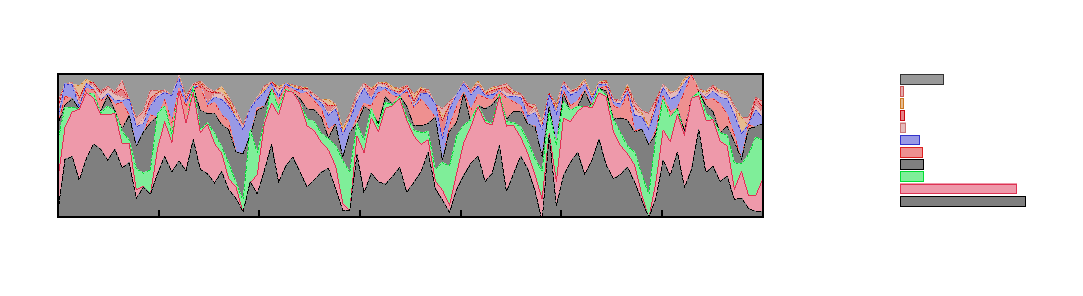
\includegraphics{img/day-vi}}%
    \gplfronttext
  \end{picture}%
\endgroup


\noindent% GNUPLOT: LaTeX picture with Postscript
\begingroup
  \makeatletter
  \providecommand\color[2][]{%
    \GenericError{(gnuplot) \space\space\space\@spaces}{%
      Package color not loaded in conjunction with
      terminal option `colourtext'%
    }{See the gnuplot documentation for explanation.%
    }{Either use 'blacktext' in gnuplot or load the package
      color.sty in LaTeX.}%
    \renewcommand\color[2][]{}%
  }%
  \providecommand\includegraphics[2][]{%
    \GenericError{(gnuplot) \space\space\space\@spaces}{%
      Package graphicx or graphics not loaded%
    }{See the gnuplot documentation for explanation.%
    }{The gnuplot epslatex terminal needs graphicx.sty or graphics.sty.}%
    \renewcommand\includegraphics[2][]{}%
  }%
  \providecommand\rotatebox[2]{#2}%
  \@ifundefined{ifGPcolor}{%
    \newif\ifGPcolor
    \GPcolorfalse
  }{}%
  \@ifundefined{ifGPblacktext}{%
    \newif\ifGPblacktext
    \GPblacktexttrue
  }{}%
  % define a \g@addto@macro without @ in the name:
  \let\gplgaddtomacro\g@addto@macro
  % define empty templates for all commands taking text:
  \gdef\gplbacktext{}%
  \gdef\gplfronttext{}%
  \makeatother
  \ifGPblacktext
    % no textcolor at all
    \def\colorrgb#1{}%
    \def\colorgray#1{}%
  \else
    % gray or color?
    \ifGPcolor
      \def\colorrgb#1{\color[rgb]{#1}}%
      \def\colorgray#1{\color[gray]{#1}}%
      \expandafter\def\csname LTw\endcsname{\color{white}}%
      \expandafter\def\csname LTb\endcsname{\color{black}}%
      \expandafter\def\csname LTa\endcsname{\color{black}}%
      \expandafter\def\csname LT0\endcsname{\color[rgb]{1,0,0}}%
      \expandafter\def\csname LT1\endcsname{\color[rgb]{0,1,0}}%
      \expandafter\def\csname LT2\endcsname{\color[rgb]{0,0,1}}%
      \expandafter\def\csname LT3\endcsname{\color[rgb]{1,0,1}}%
      \expandafter\def\csname LT4\endcsname{\color[rgb]{0,1,1}}%
      \expandafter\def\csname LT5\endcsname{\color[rgb]{1,1,0}}%
      \expandafter\def\csname LT6\endcsname{\color[rgb]{0,0,0}}%
      \expandafter\def\csname LT7\endcsname{\color[rgb]{1,0.3,0}}%
      \expandafter\def\csname LT8\endcsname{\color[rgb]{0.5,0.5,0.5}}%
    \else
      % gray
      \def\colorrgb#1{\color{black}}%
      \def\colorgray#1{\color[gray]{#1}}%
      \expandafter\def\csname LTw\endcsname{\color{white}}%
      \expandafter\def\csname LTb\endcsname{\color{black}}%
      \expandafter\def\csname LTa\endcsname{\color{black}}%
      \expandafter\def\csname LT0\endcsname{\color{black}}%
      \expandafter\def\csname LT1\endcsname{\color{black}}%
      \expandafter\def\csname LT2\endcsname{\color{black}}%
      \expandafter\def\csname LT3\endcsname{\color{black}}%
      \expandafter\def\csname LT4\endcsname{\color{black}}%
      \expandafter\def\csname LT5\endcsname{\color{black}}%
      \expandafter\def\csname LT6\endcsname{\color{black}}%
      \expandafter\def\csname LT7\endcsname{\color{black}}%
      \expandafter\def\csname LT8\endcsname{\color{black}}%
    \fi
  \fi
  \setlength{\unitlength}{0.0500bp}%
  \begin{picture}(10080.00,2520.00)%
    \gplgaddtomacro\gplbacktext{%
      \csname LTb\endcsname%
      \put(176,1281){\rotatebox{-270}{\makebox(0,0){\strut{}\scriptsize fraction of tweets}}}%
      \put(3779,154){\makebox(0,0){\strut{}\scriptsize day of week(UTC)}}%
      \put(3779,2189){\makebox(0,0){\strut{}Countries that Tweet in Thai}}%
    }%
    \gplgaddtomacro\gplfronttext{%
      \csname LTb\endcsname%
      \put(396,374){\makebox(0,0){\strut{}\scriptsize 0}}%
      \put(1363,374){\makebox(0,0){\strut{}\scriptsize 1}}%
      \put(2329,374){\makebox(0,0){\strut{}\scriptsize 2}}%
      \put(3296,374){\makebox(0,0){\strut{}\scriptsize 3}}%
      \put(4263,374){\makebox(0,0){\strut{}\scriptsize 4}}%
      \put(5230,374){\makebox(0,0){\strut{}\scriptsize 5}}%
      \put(6196,374){\makebox(0,0){\strut{}\scriptsize 6}}%
      \put(7163,374){\makebox(0,0){\strut{}\scriptsize 7}}%
    }%
    \gplgaddtomacro\gplbacktext{%
      \csname LTb\endcsname%
      \put(9083,154){\makebox(0,0){\strut{}~~}}%
      \put(9083,2189){\makebox(0,0){\strut{} }}%
    }%
    \gplgaddtomacro\gplfronttext{%
      \csname LTb\endcsname%
      \put(8352,751){\makebox(0,0)[r]{\strut{}\scriptsize~Thailand}}%
      \put(8352,868){\makebox(0,0)[r]{\strut{}\scriptsize~South~Korea}}%
      \put(8352,985){\makebox(0,0)[r]{\strut{}\scriptsize~Japan}}%
      \put(8352,1102){\makebox(0,0)[r]{\strut{}\scriptsize~USA}}%
      \put(8352,1219){\makebox(0,0)[r]{\strut{}\scriptsize~Australia}}%
      \put(8352,1337){\makebox(0,0)[r]{\strut{}\scriptsize~China}}%
      \put(8352,1454){\makebox(0,0)[r]{\strut{}\scriptsize~UK}}%
      \put(8352,1571){\makebox(0,0)[r]{\strut{}\scriptsize~Taiwan}}%
      \put(8352,1688){\makebox(0,0)[r]{\strut{}\scriptsize~Malasia}}%
      \put(8352,1805){\makebox(0,0)[r]{\strut{}\scriptsize~DE}}%
      \put(8352,1922){\makebox(0,0)[r]{\strut{}\scriptsize~other}}%
    }%
    \gplbacktext
    \put(0,0){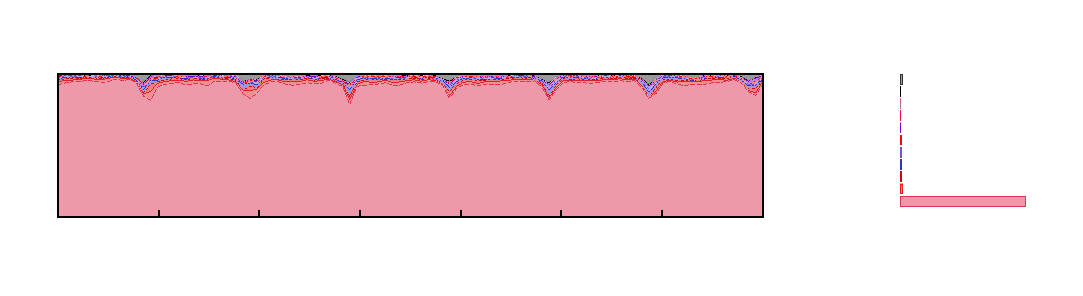
\includegraphics{img/day-th}}%
    \gplfronttext
  \end{picture}%
\endgroup


\onecolumn
\section{Languages and Time of Day}
\noindent% GNUPLOT: LaTeX picture with Postscript
\begingroup
  \makeatletter
  \providecommand\color[2][]{%
    \GenericError{(gnuplot) \space\space\space\@spaces}{%
      Package color not loaded in conjunction with
      terminal option `colourtext'%
    }{See the gnuplot documentation for explanation.%
    }{Either use 'blacktext' in gnuplot or load the package
      color.sty in LaTeX.}%
    \renewcommand\color[2][]{}%
  }%
  \providecommand\includegraphics[2][]{%
    \GenericError{(gnuplot) \space\space\space\@spaces}{%
      Package graphicx or graphics not loaded%
    }{See the gnuplot documentation for explanation.%
    }{The gnuplot epslatex terminal needs graphicx.sty or graphics.sty.}%
    \renewcommand\includegraphics[2][]{}%
  }%
  \providecommand\rotatebox[2]{#2}%
  \@ifundefined{ifGPcolor}{%
    \newif\ifGPcolor
    \GPcolorfalse
  }{}%
  \@ifundefined{ifGPblacktext}{%
    \newif\ifGPblacktext
    \GPblacktexttrue
  }{}%
  % define a \g@addto@macro without @ in the name:
  \let\gplgaddtomacro\g@addto@macro
  % define empty templates for all commands taking text:
  \gdef\gplbacktext{}%
  \gdef\gplfronttext{}%
  \makeatother
  \ifGPblacktext
    % no textcolor at all
    \def\colorrgb#1{}%
    \def\colorgray#1{}%
  \else
    % gray or color?
    \ifGPcolor
      \def\colorrgb#1{\color[rgb]{#1}}%
      \def\colorgray#1{\color[gray]{#1}}%
      \expandafter\def\csname LTw\endcsname{\color{white}}%
      \expandafter\def\csname LTb\endcsname{\color{black}}%
      \expandafter\def\csname LTa\endcsname{\color{black}}%
      \expandafter\def\csname LT0\endcsname{\color[rgb]{1,0,0}}%
      \expandafter\def\csname LT1\endcsname{\color[rgb]{0,1,0}}%
      \expandafter\def\csname LT2\endcsname{\color[rgb]{0,0,1}}%
      \expandafter\def\csname LT3\endcsname{\color[rgb]{1,0,1}}%
      \expandafter\def\csname LT4\endcsname{\color[rgb]{0,1,1}}%
      \expandafter\def\csname LT5\endcsname{\color[rgb]{1,1,0}}%
      \expandafter\def\csname LT6\endcsname{\color[rgb]{0,0,0}}%
      \expandafter\def\csname LT7\endcsname{\color[rgb]{1,0.3,0}}%
      \expandafter\def\csname LT8\endcsname{\color[rgb]{0.5,0.5,0.5}}%
    \else
      % gray
      \def\colorrgb#1{\color{black}}%
      \def\colorgray#1{\color[gray]{#1}}%
      \expandafter\def\csname LTw\endcsname{\color{white}}%
      \expandafter\def\csname LTb\endcsname{\color{black}}%
      \expandafter\def\csname LTa\endcsname{\color{black}}%
      \expandafter\def\csname LT0\endcsname{\color{black}}%
      \expandafter\def\csname LT1\endcsname{\color{black}}%
      \expandafter\def\csname LT2\endcsname{\color{black}}%
      \expandafter\def\csname LT3\endcsname{\color{black}}%
      \expandafter\def\csname LT4\endcsname{\color{black}}%
      \expandafter\def\csname LT5\endcsname{\color{black}}%
      \expandafter\def\csname LT6\endcsname{\color{black}}%
      \expandafter\def\csname LT7\endcsname{\color{black}}%
      \expandafter\def\csname LT8\endcsname{\color{black}}%
    \fi
  \fi
  \setlength{\unitlength}{0.0500bp}%
  \begin{picture}(10080.00,2520.00)%
    \gplgaddtomacro\gplbacktext{%
      \csname LTb\endcsname%
      \put(176,1281){\rotatebox{-270}{\makebox(0,0){\strut{}\scriptsize fraction of tweets}}}%
      \put(3779,154){\makebox(0,0){\strut{}\scriptsize time of day (UTC)}}%
      \put(3779,2189){\makebox(0,0){\strut{}Countries that Tweet in Arabic}}%
    }%
    \gplgaddtomacro\gplfronttext{%
      \csname LTb\endcsname%
      \put(396,374){\makebox(0,0){\strut{}\scriptsize 0:00}}%
      \put(1242,374){\makebox(0,0){\strut{}\scriptsize 3:00}}%
      \put(2088,374){\makebox(0,0){\strut{}\scriptsize 6:00}}%
      \put(2934,374){\makebox(0,0){\strut{}\scriptsize 9:00}}%
      \put(3780,374){\makebox(0,0){\strut{}\scriptsize 12:00}}%
      \put(4625,374){\makebox(0,0){\strut{}\scriptsize 15:00}}%
      \put(5471,374){\makebox(0,0){\strut{}\scriptsize 18:00}}%
      \put(6317,374){\makebox(0,0){\strut{}\scriptsize 21:00}}%
      \put(7163,374){\makebox(0,0){\strut{}\scriptsize 24:00}}%
    }%
    \gplgaddtomacro\gplbacktext{%
      \csname LTb\endcsname%
      \put(9083,154){\makebox(0,0){\strut{}~~}}%
      \put(9083,2189){\makebox(0,0){\strut{} }}%
    }%
    \gplgaddtomacro\gplfronttext{%
      \csname LTb\endcsname%
      \put(8352,751){\makebox(0,0)[r]{\strut{}\scriptsize~Saudi~Arabia}}%
      \put(8352,868){\makebox(0,0)[r]{\strut{}\scriptsize~Egypt}}%
      \put(8352,985){\makebox(0,0)[r]{\strut{}\scriptsize~Kuwait}}%
      \put(8352,1102){\makebox(0,0)[r]{\strut{}\scriptsize~Arab~Emirates}}%
      \put(8352,1219){\makebox(0,0)[r]{\strut{}\scriptsize~Qatar}}%
      \put(8352,1337){\makebox(0,0)[r]{\strut{}\scriptsize~Bahrain}}%
      \put(8352,1454){\makebox(0,0)[r]{\strut{}\scriptsize~Oman}}%
      \put(8352,1571){\makebox(0,0)[r]{\strut{}\scriptsize~USA}}%
      \put(8352,1688){\makebox(0,0)[r]{\strut{}\scriptsize~Iraq}}%
      \put(8352,1805){\makebox(0,0)[r]{\strut{}\scriptsize~UK}}%
      \put(8352,1922){\makebox(0,0)[r]{\strut{}\scriptsize~other}}%
    }%
    \gplbacktext
    \put(0,0){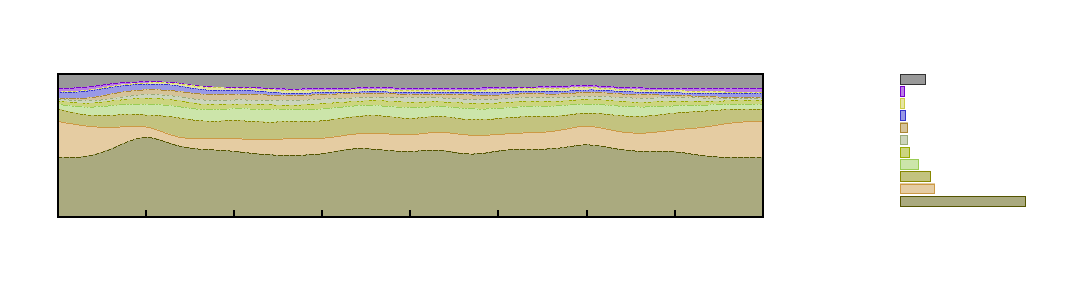
\includegraphics{img/hr-ar}}%
    \gplfronttext
  \end{picture}%
\endgroup


\noindent% GNUPLOT: LaTeX picture with Postscript
\begingroup
  \makeatletter
  \providecommand\color[2][]{%
    \GenericError{(gnuplot) \space\space\space\@spaces}{%
      Package color not loaded in conjunction with
      terminal option `colourtext'%
    }{See the gnuplot documentation for explanation.%
    }{Either use 'blacktext' in gnuplot or load the package
      color.sty in LaTeX.}%
    \renewcommand\color[2][]{}%
  }%
  \providecommand\includegraphics[2][]{%
    \GenericError{(gnuplot) \space\space\space\@spaces}{%
      Package graphicx or graphics not loaded%
    }{See the gnuplot documentation for explanation.%
    }{The gnuplot epslatex terminal needs graphicx.sty or graphics.sty.}%
    \renewcommand\includegraphics[2][]{}%
  }%
  \providecommand\rotatebox[2]{#2}%
  \@ifundefined{ifGPcolor}{%
    \newif\ifGPcolor
    \GPcolorfalse
  }{}%
  \@ifundefined{ifGPblacktext}{%
    \newif\ifGPblacktext
    \GPblacktexttrue
  }{}%
  % define a \g@addto@macro without @ in the name:
  \let\gplgaddtomacro\g@addto@macro
  % define empty templates for all commands taking text:
  \gdef\gplbacktext{}%
  \gdef\gplfronttext{}%
  \makeatother
  \ifGPblacktext
    % no textcolor at all
    \def\colorrgb#1{}%
    \def\colorgray#1{}%
  \else
    % gray or color?
    \ifGPcolor
      \def\colorrgb#1{\color[rgb]{#1}}%
      \def\colorgray#1{\color[gray]{#1}}%
      \expandafter\def\csname LTw\endcsname{\color{white}}%
      \expandafter\def\csname LTb\endcsname{\color{black}}%
      \expandafter\def\csname LTa\endcsname{\color{black}}%
      \expandafter\def\csname LT0\endcsname{\color[rgb]{1,0,0}}%
      \expandafter\def\csname LT1\endcsname{\color[rgb]{0,1,0}}%
      \expandafter\def\csname LT2\endcsname{\color[rgb]{0,0,1}}%
      \expandafter\def\csname LT3\endcsname{\color[rgb]{1,0,1}}%
      \expandafter\def\csname LT4\endcsname{\color[rgb]{0,1,1}}%
      \expandafter\def\csname LT5\endcsname{\color[rgb]{1,1,0}}%
      \expandafter\def\csname LT6\endcsname{\color[rgb]{0,0,0}}%
      \expandafter\def\csname LT7\endcsname{\color[rgb]{1,0.3,0}}%
      \expandafter\def\csname LT8\endcsname{\color[rgb]{0.5,0.5,0.5}}%
    \else
      % gray
      \def\colorrgb#1{\color{black}}%
      \def\colorgray#1{\color[gray]{#1}}%
      \expandafter\def\csname LTw\endcsname{\color{white}}%
      \expandafter\def\csname LTb\endcsname{\color{black}}%
      \expandafter\def\csname LTa\endcsname{\color{black}}%
      \expandafter\def\csname LT0\endcsname{\color{black}}%
      \expandafter\def\csname LT1\endcsname{\color{black}}%
      \expandafter\def\csname LT2\endcsname{\color{black}}%
      \expandafter\def\csname LT3\endcsname{\color{black}}%
      \expandafter\def\csname LT4\endcsname{\color{black}}%
      \expandafter\def\csname LT5\endcsname{\color{black}}%
      \expandafter\def\csname LT6\endcsname{\color{black}}%
      \expandafter\def\csname LT7\endcsname{\color{black}}%
      \expandafter\def\csname LT8\endcsname{\color{black}}%
    \fi
  \fi
  \setlength{\unitlength}{0.0500bp}%
  \begin{picture}(10080.00,2520.00)%
    \gplgaddtomacro\gplbacktext{%
      \csname LTb\endcsname%
      \put(176,1281){\rotatebox{-270}{\makebox(0,0){\strut{}\scriptsize fraction of tweets}}}%
      \put(3779,154){\makebox(0,0){\strut{}\scriptsize time of day (UTC)}}%
      \put(3779,2189){\makebox(0,0){\strut{}Countries that Tweet in English}}%
    }%
    \gplgaddtomacro\gplfronttext{%
      \csname LTb\endcsname%
      \put(396,374){\makebox(0,0){\strut{}\scriptsize 0:00}}%
      \put(1242,374){\makebox(0,0){\strut{}\scriptsize 3:00}}%
      \put(2088,374){\makebox(0,0){\strut{}\scriptsize 6:00}}%
      \put(2934,374){\makebox(0,0){\strut{}\scriptsize 9:00}}%
      \put(3780,374){\makebox(0,0){\strut{}\scriptsize 12:00}}%
      \put(4625,374){\makebox(0,0){\strut{}\scriptsize 15:00}}%
      \put(5471,374){\makebox(0,0){\strut{}\scriptsize 18:00}}%
      \put(6317,374){\makebox(0,0){\strut{}\scriptsize 21:00}}%
      \put(7163,374){\makebox(0,0){\strut{}\scriptsize 24:00}}%
    }%
    \gplgaddtomacro\gplbacktext{%
      \csname LTb\endcsname%
      \put(9083,154){\makebox(0,0){\strut{}~~}}%
      \put(9083,2189){\makebox(0,0){\strut{} }}%
    }%
    \gplgaddtomacro\gplfronttext{%
      \csname LTb\endcsname%
      \put(8352,751){\makebox(0,0)[r]{\strut{}\scriptsize~USA}}%
      \put(8352,868){\makebox(0,0)[r]{\strut{}\scriptsize~UK}}%
      \put(8352,985){\makebox(0,0)[r]{\strut{}\scriptsize~Philippines}}%
      \put(8352,1102){\makebox(0,0)[r]{\strut{}\scriptsize~Canada}}%
      \put(8352,1219){\makebox(0,0)[r]{\strut{}\scriptsize~India}}%
      \put(8352,1337){\makebox(0,0)[r]{\strut{}\scriptsize~South~Africa}}%
      \put(8352,1454){\makebox(0,0)[r]{\strut{}\scriptsize~Australia}}%
      \put(8352,1571){\makebox(0,0)[r]{\strut{}\scriptsize~Malasia}}%
      \put(8352,1688){\makebox(0,0)[r]{\strut{}\scriptsize~Nigeria}}%
      \put(8352,1805){\makebox(0,0)[r]{\strut{}\scriptsize~Brazil}}%
      \put(8352,1922){\makebox(0,0)[r]{\strut{}\scriptsize~other}}%
    }%
    \gplbacktext
    \put(0,0){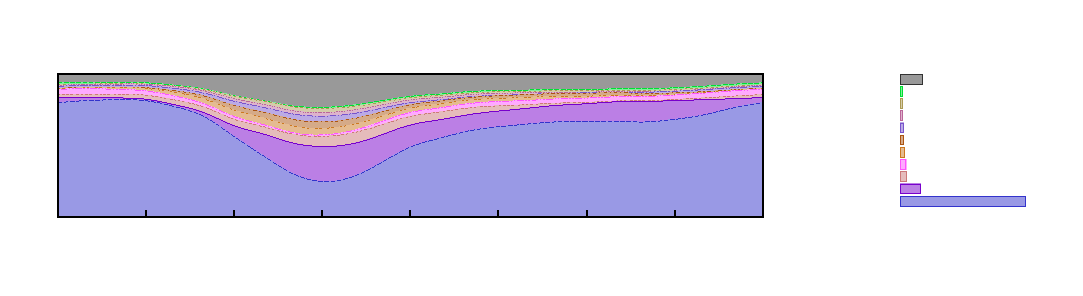
\includegraphics{img/hr-en}}%
    \gplfronttext
  \end{picture}%
\endgroup


\noindent% GNUPLOT: LaTeX picture with Postscript
\begingroup
  \makeatletter
  \providecommand\color[2][]{%
    \GenericError{(gnuplot) \space\space\space\@spaces}{%
      Package color not loaded in conjunction with
      terminal option `colourtext'%
    }{See the gnuplot documentation for explanation.%
    }{Either use 'blacktext' in gnuplot or load the package
      color.sty in LaTeX.}%
    \renewcommand\color[2][]{}%
  }%
  \providecommand\includegraphics[2][]{%
    \GenericError{(gnuplot) \space\space\space\@spaces}{%
      Package graphicx or graphics not loaded%
    }{See the gnuplot documentation for explanation.%
    }{The gnuplot epslatex terminal needs graphicx.sty or graphics.sty.}%
    \renewcommand\includegraphics[2][]{}%
  }%
  \providecommand\rotatebox[2]{#2}%
  \@ifundefined{ifGPcolor}{%
    \newif\ifGPcolor
    \GPcolorfalse
  }{}%
  \@ifundefined{ifGPblacktext}{%
    \newif\ifGPblacktext
    \GPblacktexttrue
  }{}%
  % define a \g@addto@macro without @ in the name:
  \let\gplgaddtomacro\g@addto@macro
  % define empty templates for all commands taking text:
  \gdef\gplbacktext{}%
  \gdef\gplfronttext{}%
  \makeatother
  \ifGPblacktext
    % no textcolor at all
    \def\colorrgb#1{}%
    \def\colorgray#1{}%
  \else
    % gray or color?
    \ifGPcolor
      \def\colorrgb#1{\color[rgb]{#1}}%
      \def\colorgray#1{\color[gray]{#1}}%
      \expandafter\def\csname LTw\endcsname{\color{white}}%
      \expandafter\def\csname LTb\endcsname{\color{black}}%
      \expandafter\def\csname LTa\endcsname{\color{black}}%
      \expandafter\def\csname LT0\endcsname{\color[rgb]{1,0,0}}%
      \expandafter\def\csname LT1\endcsname{\color[rgb]{0,1,0}}%
      \expandafter\def\csname LT2\endcsname{\color[rgb]{0,0,1}}%
      \expandafter\def\csname LT3\endcsname{\color[rgb]{1,0,1}}%
      \expandafter\def\csname LT4\endcsname{\color[rgb]{0,1,1}}%
      \expandafter\def\csname LT5\endcsname{\color[rgb]{1,1,0}}%
      \expandafter\def\csname LT6\endcsname{\color[rgb]{0,0,0}}%
      \expandafter\def\csname LT7\endcsname{\color[rgb]{1,0.3,0}}%
      \expandafter\def\csname LT8\endcsname{\color[rgb]{0.5,0.5,0.5}}%
    \else
      % gray
      \def\colorrgb#1{\color{black}}%
      \def\colorgray#1{\color[gray]{#1}}%
      \expandafter\def\csname LTw\endcsname{\color{white}}%
      \expandafter\def\csname LTb\endcsname{\color{black}}%
      \expandafter\def\csname LTa\endcsname{\color{black}}%
      \expandafter\def\csname LT0\endcsname{\color{black}}%
      \expandafter\def\csname LT1\endcsname{\color{black}}%
      \expandafter\def\csname LT2\endcsname{\color{black}}%
      \expandafter\def\csname LT3\endcsname{\color{black}}%
      \expandafter\def\csname LT4\endcsname{\color{black}}%
      \expandafter\def\csname LT5\endcsname{\color{black}}%
      \expandafter\def\csname LT6\endcsname{\color{black}}%
      \expandafter\def\csname LT7\endcsname{\color{black}}%
      \expandafter\def\csname LT8\endcsname{\color{black}}%
    \fi
  \fi
  \setlength{\unitlength}{0.0500bp}%
  \begin{picture}(10080.00,2520.00)%
    \gplgaddtomacro\gplbacktext{%
      \csname LTb\endcsname%
      \put(176,1281){\rotatebox{-270}{\makebox(0,0){\strut{}\scriptsize fraction of tweets}}}%
      \put(3779,154){\makebox(0,0){\strut{}\scriptsize time of day (UTC)}}%
      \put(3779,2189){\makebox(0,0){\strut{}Countries that Tweet in Spanish}}%
    }%
    \gplgaddtomacro\gplfronttext{%
      \csname LTb\endcsname%
      \put(396,374){\makebox(0,0){\strut{}\scriptsize 0:00}}%
      \put(1242,374){\makebox(0,0){\strut{}\scriptsize 3:00}}%
      \put(2088,374){\makebox(0,0){\strut{}\scriptsize 6:00}}%
      \put(2934,374){\makebox(0,0){\strut{}\scriptsize 9:00}}%
      \put(3780,374){\makebox(0,0){\strut{}\scriptsize 12:00}}%
      \put(4625,374){\makebox(0,0){\strut{}\scriptsize 15:00}}%
      \put(5471,374){\makebox(0,0){\strut{}\scriptsize 18:00}}%
      \put(6317,374){\makebox(0,0){\strut{}\scriptsize 21:00}}%
      \put(7163,374){\makebox(0,0){\strut{}\scriptsize 24:00}}%
    }%
    \gplgaddtomacro\gplbacktext{%
      \csname LTb\endcsname%
      \put(9083,154){\makebox(0,0){\strut{}~~}}%
      \put(9083,2189){\makebox(0,0){\strut{} }}%
    }%
    \gplgaddtomacro\gplfronttext{%
      \csname LTb\endcsname%
      \put(8352,751){\makebox(0,0)[r]{\strut{}\scriptsize~Argentina}}%
      \put(8352,868){\makebox(0,0)[r]{\strut{}\scriptsize~Spain}}%
      \put(8352,985){\makebox(0,0)[r]{\strut{}\scriptsize~Mexico}}%
      \put(8352,1102){\makebox(0,0)[r]{\strut{}\scriptsize~Colombia}}%
      \put(8352,1219){\makebox(0,0)[r]{\strut{}\scriptsize~Chile}}%
      \put(8352,1337){\makebox(0,0)[r]{\strut{}\scriptsize~USA}}%
      \put(8352,1454){\makebox(0,0)[r]{\strut{}\scriptsize~Venezuela}}%
      \put(8352,1571){\makebox(0,0)[r]{\strut{}\scriptsize~Brazil}}%
      \put(8352,1688){\makebox(0,0)[r]{\strut{}\scriptsize~Uruguay}}%
      \put(8352,1805){\makebox(0,0)[r]{\strut{}\scriptsize~PE}}%
      \put(8352,1922){\makebox(0,0)[r]{\strut{}\scriptsize~other}}%
    }%
    \gplbacktext
    \put(0,0){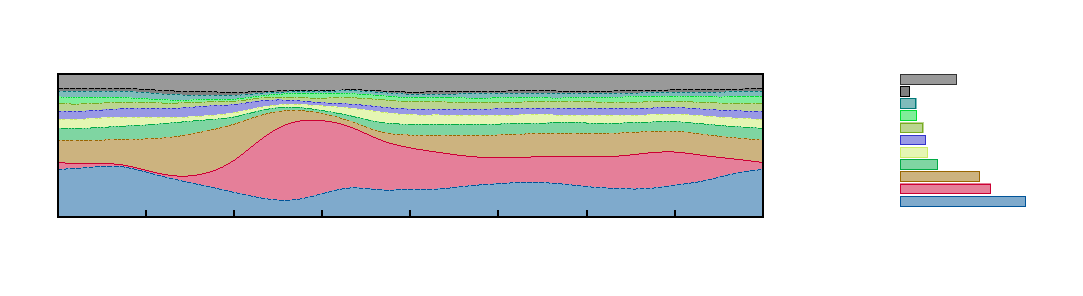
\includegraphics{img/hr-es}}%
    \gplfronttext
  \end{picture}%
\endgroup


\noindent% GNUPLOT: LaTeX picture with Postscript
\begingroup
  \makeatletter
  \providecommand\color[2][]{%
    \GenericError{(gnuplot) \space\space\space\@spaces}{%
      Package color not loaded in conjunction with
      terminal option `colourtext'%
    }{See the gnuplot documentation for explanation.%
    }{Either use 'blacktext' in gnuplot or load the package
      color.sty in LaTeX.}%
    \renewcommand\color[2][]{}%
  }%
  \providecommand\includegraphics[2][]{%
    \GenericError{(gnuplot) \space\space\space\@spaces}{%
      Package graphicx or graphics not loaded%
    }{See the gnuplot documentation for explanation.%
    }{The gnuplot epslatex terminal needs graphicx.sty or graphics.sty.}%
    \renewcommand\includegraphics[2][]{}%
  }%
  \providecommand\rotatebox[2]{#2}%
  \@ifundefined{ifGPcolor}{%
    \newif\ifGPcolor
    \GPcolorfalse
  }{}%
  \@ifundefined{ifGPblacktext}{%
    \newif\ifGPblacktext
    \GPblacktexttrue
  }{}%
  % define a \g@addto@macro without @ in the name:
  \let\gplgaddtomacro\g@addto@macro
  % define empty templates for all commands taking text:
  \gdef\gplbacktext{}%
  \gdef\gplfronttext{}%
  \makeatother
  \ifGPblacktext
    % no textcolor at all
    \def\colorrgb#1{}%
    \def\colorgray#1{}%
  \else
    % gray or color?
    \ifGPcolor
      \def\colorrgb#1{\color[rgb]{#1}}%
      \def\colorgray#1{\color[gray]{#1}}%
      \expandafter\def\csname LTw\endcsname{\color{white}}%
      \expandafter\def\csname LTb\endcsname{\color{black}}%
      \expandafter\def\csname LTa\endcsname{\color{black}}%
      \expandafter\def\csname LT0\endcsname{\color[rgb]{1,0,0}}%
      \expandafter\def\csname LT1\endcsname{\color[rgb]{0,1,0}}%
      \expandafter\def\csname LT2\endcsname{\color[rgb]{0,0,1}}%
      \expandafter\def\csname LT3\endcsname{\color[rgb]{1,0,1}}%
      \expandafter\def\csname LT4\endcsname{\color[rgb]{0,1,1}}%
      \expandafter\def\csname LT5\endcsname{\color[rgb]{1,1,0}}%
      \expandafter\def\csname LT6\endcsname{\color[rgb]{0,0,0}}%
      \expandafter\def\csname LT7\endcsname{\color[rgb]{1,0.3,0}}%
      \expandafter\def\csname LT8\endcsname{\color[rgb]{0.5,0.5,0.5}}%
    \else
      % gray
      \def\colorrgb#1{\color{black}}%
      \def\colorgray#1{\color[gray]{#1}}%
      \expandafter\def\csname LTw\endcsname{\color{white}}%
      \expandafter\def\csname LTb\endcsname{\color{black}}%
      \expandafter\def\csname LTa\endcsname{\color{black}}%
      \expandafter\def\csname LT0\endcsname{\color{black}}%
      \expandafter\def\csname LT1\endcsname{\color{black}}%
      \expandafter\def\csname LT2\endcsname{\color{black}}%
      \expandafter\def\csname LT3\endcsname{\color{black}}%
      \expandafter\def\csname LT4\endcsname{\color{black}}%
      \expandafter\def\csname LT5\endcsname{\color{black}}%
      \expandafter\def\csname LT6\endcsname{\color{black}}%
      \expandafter\def\csname LT7\endcsname{\color{black}}%
      \expandafter\def\csname LT8\endcsname{\color{black}}%
    \fi
  \fi
  \setlength{\unitlength}{0.0500bp}%
  \begin{picture}(10080.00,2520.00)%
    \gplgaddtomacro\gplbacktext{%
      \csname LTb\endcsname%
      \put(176,1281){\rotatebox{-270}{\makebox(0,0){\strut{}\scriptsize fraction of tweets}}}%
      \put(3779,154){\makebox(0,0){\strut{}\scriptsize time of day (UTC)}}%
      \put(3779,2189){\makebox(0,0){\strut{}Countries that Tweet in French}}%
    }%
    \gplgaddtomacro\gplfronttext{%
      \csname LTb\endcsname%
      \put(396,374){\makebox(0,0){\strut{}\scriptsize 0:00}}%
      \put(1242,374){\makebox(0,0){\strut{}\scriptsize 3:00}}%
      \put(2088,374){\makebox(0,0){\strut{}\scriptsize 6:00}}%
      \put(2934,374){\makebox(0,0){\strut{}\scriptsize 9:00}}%
      \put(3780,374){\makebox(0,0){\strut{}\scriptsize 12:00}}%
      \put(4625,374){\makebox(0,0){\strut{}\scriptsize 15:00}}%
      \put(5471,374){\makebox(0,0){\strut{}\scriptsize 18:00}}%
      \put(6317,374){\makebox(0,0){\strut{}\scriptsize 21:00}}%
      \put(7163,374){\makebox(0,0){\strut{}\scriptsize 24:00}}%
    }%
    \gplgaddtomacro\gplbacktext{%
      \csname LTb\endcsname%
      \put(9083,154){\makebox(0,0){\strut{}~~}}%
      \put(9083,2189){\makebox(0,0){\strut{} }}%
    }%
    \gplgaddtomacro\gplfronttext{%
      \csname LTb\endcsname%
      \put(8352,751){\makebox(0,0)[r]{\strut{}\scriptsize~France}}%
      \put(8352,868){\makebox(0,0)[r]{\strut{}\scriptsize~USA}}%
      \put(8352,985){\makebox(0,0)[r]{\strut{}\scriptsize~Canada}}%
      \put(8352,1102){\makebox(0,0)[r]{\strut{}\scriptsize~Belgium}}%
      \put(8352,1219){\makebox(0,0)[r]{\strut{}\scriptsize~Brazil}}%
      \put(8352,1337){\makebox(0,0)[r]{\strut{}\scriptsize~UK}}%
      \put(8352,1454){\makebox(0,0)[r]{\strut{}\scriptsize~Spain}}%
      \put(8352,1571){\makebox(0,0)[r]{\strut{}\scriptsize~Switzerland}}%
      \put(8352,1688){\makebox(0,0)[r]{\strut{}\scriptsize~Cameroon}}%
      \put(8352,1805){\makebox(0,0)[r]{\strut{}\scriptsize~Cote~d'Ivoire}}%
      \put(8352,1922){\makebox(0,0)[r]{\strut{}\scriptsize~other}}%
    }%
    \gplbacktext
    \put(0,0){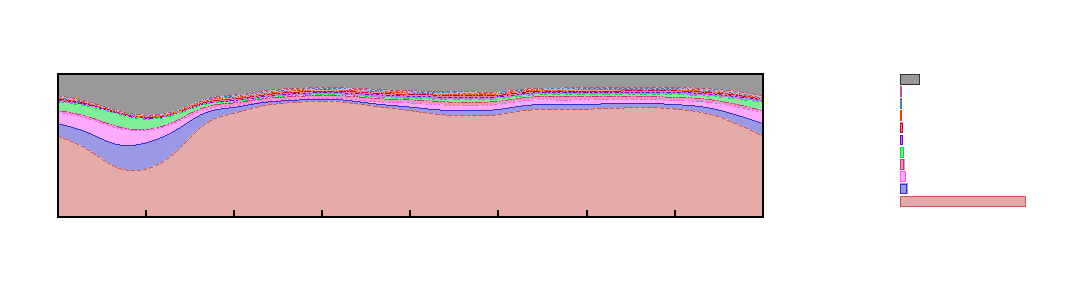
\includegraphics{img/hr-fr}}%
    \gplfronttext
  \end{picture}%
\endgroup


\noindent% GNUPLOT: LaTeX picture with Postscript
\begingroup
  \makeatletter
  \providecommand\color[2][]{%
    \GenericError{(gnuplot) \space\space\space\@spaces}{%
      Package color not loaded in conjunction with
      terminal option `colourtext'%
    }{See the gnuplot documentation for explanation.%
    }{Either use 'blacktext' in gnuplot or load the package
      color.sty in LaTeX.}%
    \renewcommand\color[2][]{}%
  }%
  \providecommand\includegraphics[2][]{%
    \GenericError{(gnuplot) \space\space\space\@spaces}{%
      Package graphicx or graphics not loaded%
    }{See the gnuplot documentation for explanation.%
    }{The gnuplot epslatex terminal needs graphicx.sty or graphics.sty.}%
    \renewcommand\includegraphics[2][]{}%
  }%
  \providecommand\rotatebox[2]{#2}%
  \@ifundefined{ifGPcolor}{%
    \newif\ifGPcolor
    \GPcolorfalse
  }{}%
  \@ifundefined{ifGPblacktext}{%
    \newif\ifGPblacktext
    \GPblacktexttrue
  }{}%
  % define a \g@addto@macro without @ in the name:
  \let\gplgaddtomacro\g@addto@macro
  % define empty templates for all commands taking text:
  \gdef\gplbacktext{}%
  \gdef\gplfronttext{}%
  \makeatother
  \ifGPblacktext
    % no textcolor at all
    \def\colorrgb#1{}%
    \def\colorgray#1{}%
  \else
    % gray or color?
    \ifGPcolor
      \def\colorrgb#1{\color[rgb]{#1}}%
      \def\colorgray#1{\color[gray]{#1}}%
      \expandafter\def\csname LTw\endcsname{\color{white}}%
      \expandafter\def\csname LTb\endcsname{\color{black}}%
      \expandafter\def\csname LTa\endcsname{\color{black}}%
      \expandafter\def\csname LT0\endcsname{\color[rgb]{1,0,0}}%
      \expandafter\def\csname LT1\endcsname{\color[rgb]{0,1,0}}%
      \expandafter\def\csname LT2\endcsname{\color[rgb]{0,0,1}}%
      \expandafter\def\csname LT3\endcsname{\color[rgb]{1,0,1}}%
      \expandafter\def\csname LT4\endcsname{\color[rgb]{0,1,1}}%
      \expandafter\def\csname LT5\endcsname{\color[rgb]{1,1,0}}%
      \expandafter\def\csname LT6\endcsname{\color[rgb]{0,0,0}}%
      \expandafter\def\csname LT7\endcsname{\color[rgb]{1,0.3,0}}%
      \expandafter\def\csname LT8\endcsname{\color[rgb]{0.5,0.5,0.5}}%
    \else
      % gray
      \def\colorrgb#1{\color{black}}%
      \def\colorgray#1{\color[gray]{#1}}%
      \expandafter\def\csname LTw\endcsname{\color{white}}%
      \expandafter\def\csname LTb\endcsname{\color{black}}%
      \expandafter\def\csname LTa\endcsname{\color{black}}%
      \expandafter\def\csname LT0\endcsname{\color{black}}%
      \expandafter\def\csname LT1\endcsname{\color{black}}%
      \expandafter\def\csname LT2\endcsname{\color{black}}%
      \expandafter\def\csname LT3\endcsname{\color{black}}%
      \expandafter\def\csname LT4\endcsname{\color{black}}%
      \expandafter\def\csname LT5\endcsname{\color{black}}%
      \expandafter\def\csname LT6\endcsname{\color{black}}%
      \expandafter\def\csname LT7\endcsname{\color{black}}%
      \expandafter\def\csname LT8\endcsname{\color{black}}%
    \fi
  \fi
  \setlength{\unitlength}{0.0500bp}%
  \begin{picture}(10080.00,2520.00)%
    \gplgaddtomacro\gplbacktext{%
      \csname LTb\endcsname%
      \put(176,1281){\rotatebox{-270}{\makebox(0,0){\strut{}\scriptsize fraction of tweets}}}%
      \put(3779,154){\makebox(0,0){\strut{}\scriptsize time of day (UTC)}}%
      \put(3779,2189){\makebox(0,0){\strut{}Countries that Tweet in Indonesian}}%
    }%
    \gplgaddtomacro\gplfronttext{%
      \csname LTb\endcsname%
      \put(396,374){\makebox(0,0){\strut{}\scriptsize 0:00}}%
      \put(1242,374){\makebox(0,0){\strut{}\scriptsize 3:00}}%
      \put(2088,374){\makebox(0,0){\strut{}\scriptsize 6:00}}%
      \put(2934,374){\makebox(0,0){\strut{}\scriptsize 9:00}}%
      \put(3780,374){\makebox(0,0){\strut{}\scriptsize 12:00}}%
      \put(4625,374){\makebox(0,0){\strut{}\scriptsize 15:00}}%
      \put(5471,374){\makebox(0,0){\strut{}\scriptsize 18:00}}%
      \put(6317,374){\makebox(0,0){\strut{}\scriptsize 21:00}}%
      \put(7163,374){\makebox(0,0){\strut{}\scriptsize 24:00}}%
    }%
    \gplgaddtomacro\gplbacktext{%
      \csname LTb\endcsname%
      \put(9083,154){\makebox(0,0){\strut{}~~}}%
      \put(9083,2189){\makebox(0,0){\strut{} }}%
    }%
    \gplgaddtomacro\gplfronttext{%
      \csname LTb\endcsname%
      \put(8352,751){\makebox(0,0)[r]{\strut{}\scriptsize~Malasia}}%
      \put(8352,868){\makebox(0,0)[r]{\strut{}\scriptsize~Indonesia}}%
      \put(8352,985){\makebox(0,0)[r]{\strut{}\scriptsize~Philippines}}%
      \put(8352,1102){\makebox(0,0)[r]{\strut{}\scriptsize~USA}}%
      \put(8352,1219){\makebox(0,0)[r]{\strut{}\scriptsize~Brazil}}%
      \put(8352,1337){\makebox(0,0)[r]{\strut{}\scriptsize~India}}%
      \put(8352,1454){\makebox(0,0)[r]{\strut{}\scriptsize~South~Africa}}%
      \put(8352,1571){\makebox(0,0)[r]{\strut{}\scriptsize~Thailand}}%
      \put(8352,1688){\makebox(0,0)[r]{\strut{}\scriptsize~Japan}}%
      \put(8352,1805){\makebox(0,0)[r]{\strut{}\scriptsize~TR}}%
      \put(8352,1922){\makebox(0,0)[r]{\strut{}\scriptsize~other}}%
    }%
    \gplbacktext
    \put(0,0){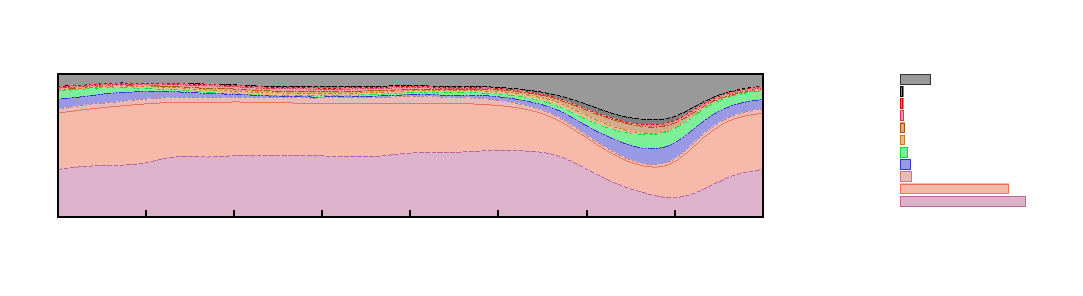
\includegraphics{img/hr-in}}%
    \gplfronttext
  \end{picture}%
\endgroup


\noindent% GNUPLOT: LaTeX picture with Postscript
\begingroup
  \makeatletter
  \providecommand\color[2][]{%
    \GenericError{(gnuplot) \space\space\space\@spaces}{%
      Package color not loaded in conjunction with
      terminal option `colourtext'%
    }{See the gnuplot documentation for explanation.%
    }{Either use 'blacktext' in gnuplot or load the package
      color.sty in LaTeX.}%
    \renewcommand\color[2][]{}%
  }%
  \providecommand\includegraphics[2][]{%
    \GenericError{(gnuplot) \space\space\space\@spaces}{%
      Package graphicx or graphics not loaded%
    }{See the gnuplot documentation for explanation.%
    }{The gnuplot epslatex terminal needs graphicx.sty or graphics.sty.}%
    \renewcommand\includegraphics[2][]{}%
  }%
  \providecommand\rotatebox[2]{#2}%
  \@ifundefined{ifGPcolor}{%
    \newif\ifGPcolor
    \GPcolorfalse
  }{}%
  \@ifundefined{ifGPblacktext}{%
    \newif\ifGPblacktext
    \GPblacktexttrue
  }{}%
  % define a \g@addto@macro without @ in the name:
  \let\gplgaddtomacro\g@addto@macro
  % define empty templates for all commands taking text:
  \gdef\gplbacktext{}%
  \gdef\gplfronttext{}%
  \makeatother
  \ifGPblacktext
    % no textcolor at all
    \def\colorrgb#1{}%
    \def\colorgray#1{}%
  \else
    % gray or color?
    \ifGPcolor
      \def\colorrgb#1{\color[rgb]{#1}}%
      \def\colorgray#1{\color[gray]{#1}}%
      \expandafter\def\csname LTw\endcsname{\color{white}}%
      \expandafter\def\csname LTb\endcsname{\color{black}}%
      \expandafter\def\csname LTa\endcsname{\color{black}}%
      \expandafter\def\csname LT0\endcsname{\color[rgb]{1,0,0}}%
      \expandafter\def\csname LT1\endcsname{\color[rgb]{0,1,0}}%
      \expandafter\def\csname LT2\endcsname{\color[rgb]{0,0,1}}%
      \expandafter\def\csname LT3\endcsname{\color[rgb]{1,0,1}}%
      \expandafter\def\csname LT4\endcsname{\color[rgb]{0,1,1}}%
      \expandafter\def\csname LT5\endcsname{\color[rgb]{1,1,0}}%
      \expandafter\def\csname LT6\endcsname{\color[rgb]{0,0,0}}%
      \expandafter\def\csname LT7\endcsname{\color[rgb]{1,0.3,0}}%
      \expandafter\def\csname LT8\endcsname{\color[rgb]{0.5,0.5,0.5}}%
    \else
      % gray
      \def\colorrgb#1{\color{black}}%
      \def\colorgray#1{\color[gray]{#1}}%
      \expandafter\def\csname LTw\endcsname{\color{white}}%
      \expandafter\def\csname LTb\endcsname{\color{black}}%
      \expandafter\def\csname LTa\endcsname{\color{black}}%
      \expandafter\def\csname LT0\endcsname{\color{black}}%
      \expandafter\def\csname LT1\endcsname{\color{black}}%
      \expandafter\def\csname LT2\endcsname{\color{black}}%
      \expandafter\def\csname LT3\endcsname{\color{black}}%
      \expandafter\def\csname LT4\endcsname{\color{black}}%
      \expandafter\def\csname LT5\endcsname{\color{black}}%
      \expandafter\def\csname LT6\endcsname{\color{black}}%
      \expandafter\def\csname LT7\endcsname{\color{black}}%
      \expandafter\def\csname LT8\endcsname{\color{black}}%
    \fi
  \fi
  \setlength{\unitlength}{0.0500bp}%
  \begin{picture}(10080.00,2520.00)%
    \gplgaddtomacro\gplbacktext{%
      \csname LTb\endcsname%
      \put(176,1281){\rotatebox{-270}{\makebox(0,0){\strut{}\scriptsize fraction of tweets}}}%
      \put(3779,154){\makebox(0,0){\strut{}\scriptsize time of day (UTC)}}%
      \put(3779,2189){\makebox(0,0){\strut{}Countries that Tweet in Tagalog}}%
    }%
    \gplgaddtomacro\gplfronttext{%
      \csname LTb\endcsname%
      \put(396,374){\makebox(0,0){\strut{}\scriptsize 0:00}}%
      \put(1242,374){\makebox(0,0){\strut{}\scriptsize 3:00}}%
      \put(2088,374){\makebox(0,0){\strut{}\scriptsize 6:00}}%
      \put(2934,374){\makebox(0,0){\strut{}\scriptsize 9:00}}%
      \put(3780,374){\makebox(0,0){\strut{}\scriptsize 12:00}}%
      \put(4625,374){\makebox(0,0){\strut{}\scriptsize 15:00}}%
      \put(5471,374){\makebox(0,0){\strut{}\scriptsize 18:00}}%
      \put(6317,374){\makebox(0,0){\strut{}\scriptsize 21:00}}%
      \put(7163,374){\makebox(0,0){\strut{}\scriptsize 24:00}}%
    }%
    \gplgaddtomacro\gplbacktext{%
      \csname LTb\endcsname%
      \put(9083,154){\makebox(0,0){\strut{}~~}}%
      \put(9083,2189){\makebox(0,0){\strut{} }}%
    }%
    \gplgaddtomacro\gplfronttext{%
      \csname LTb\endcsname%
      \put(8352,751){\makebox(0,0)[r]{\strut{}\scriptsize~Philippines}}%
      \put(8352,868){\makebox(0,0)[r]{\strut{}\scriptsize~USA}}%
      \put(8352,985){\makebox(0,0)[r]{\strut{}\scriptsize~Malasia}}%
      \put(8352,1102){\makebox(0,0)[r]{\strut{}\scriptsize~Brazil}}%
      \put(8352,1219){\makebox(0,0)[r]{\strut{}\scriptsize~Indonesia}}%
      \put(8352,1337){\makebox(0,0)[r]{\strut{}\scriptsize~South~Africa}}%
      \put(8352,1454){\makebox(0,0)[r]{\strut{}\scriptsize~India}}%
      \put(8352,1571){\makebox(0,0)[r]{\strut{}\scriptsize~UK}}%
      \put(8352,1688){\makebox(0,0)[r]{\strut{}\scriptsize~Canada}}%
      \put(8352,1805){\makebox(0,0)[r]{\strut{}\scriptsize~Japan}}%
      \put(8352,1922){\makebox(0,0)[r]{\strut{}\scriptsize~other}}%
    }%
    \gplbacktext
    \put(0,0){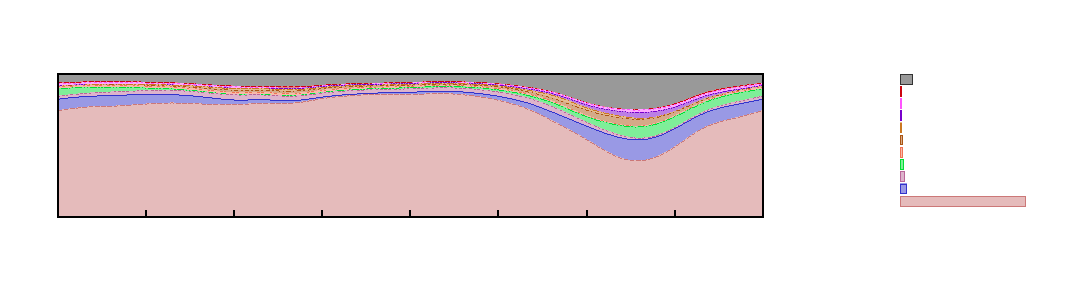
\includegraphics{img/hr-tl}}%
    \gplfronttext
  \end{picture}%
\endgroup


\noindent% GNUPLOT: LaTeX picture with Postscript
\begingroup
  \makeatletter
  \providecommand\color[2][]{%
    \GenericError{(gnuplot) \space\space\space\@spaces}{%
      Package color not loaded in conjunction with
      terminal option `colourtext'%
    }{See the gnuplot documentation for explanation.%
    }{Either use 'blacktext' in gnuplot or load the package
      color.sty in LaTeX.}%
    \renewcommand\color[2][]{}%
  }%
  \providecommand\includegraphics[2][]{%
    \GenericError{(gnuplot) \space\space\space\@spaces}{%
      Package graphicx or graphics not loaded%
    }{See the gnuplot documentation for explanation.%
    }{The gnuplot epslatex terminal needs graphicx.sty or graphics.sty.}%
    \renewcommand\includegraphics[2][]{}%
  }%
  \providecommand\rotatebox[2]{#2}%
  \@ifundefined{ifGPcolor}{%
    \newif\ifGPcolor
    \GPcolorfalse
  }{}%
  \@ifundefined{ifGPblacktext}{%
    \newif\ifGPblacktext
    \GPblacktexttrue
  }{}%
  % define a \g@addto@macro without @ in the name:
  \let\gplgaddtomacro\g@addto@macro
  % define empty templates for all commands taking text:
  \gdef\gplbacktext{}%
  \gdef\gplfronttext{}%
  \makeatother
  \ifGPblacktext
    % no textcolor at all
    \def\colorrgb#1{}%
    \def\colorgray#1{}%
  \else
    % gray or color?
    \ifGPcolor
      \def\colorrgb#1{\color[rgb]{#1}}%
      \def\colorgray#1{\color[gray]{#1}}%
      \expandafter\def\csname LTw\endcsname{\color{white}}%
      \expandafter\def\csname LTb\endcsname{\color{black}}%
      \expandafter\def\csname LTa\endcsname{\color{black}}%
      \expandafter\def\csname LT0\endcsname{\color[rgb]{1,0,0}}%
      \expandafter\def\csname LT1\endcsname{\color[rgb]{0,1,0}}%
      \expandafter\def\csname LT2\endcsname{\color[rgb]{0,0,1}}%
      \expandafter\def\csname LT3\endcsname{\color[rgb]{1,0,1}}%
      \expandafter\def\csname LT4\endcsname{\color[rgb]{0,1,1}}%
      \expandafter\def\csname LT5\endcsname{\color[rgb]{1,1,0}}%
      \expandafter\def\csname LT6\endcsname{\color[rgb]{0,0,0}}%
      \expandafter\def\csname LT7\endcsname{\color[rgb]{1,0.3,0}}%
      \expandafter\def\csname LT8\endcsname{\color[rgb]{0.5,0.5,0.5}}%
    \else
      % gray
      \def\colorrgb#1{\color{black}}%
      \def\colorgray#1{\color[gray]{#1}}%
      \expandafter\def\csname LTw\endcsname{\color{white}}%
      \expandafter\def\csname LTb\endcsname{\color{black}}%
      \expandafter\def\csname LTa\endcsname{\color{black}}%
      \expandafter\def\csname LT0\endcsname{\color{black}}%
      \expandafter\def\csname LT1\endcsname{\color{black}}%
      \expandafter\def\csname LT2\endcsname{\color{black}}%
      \expandafter\def\csname LT3\endcsname{\color{black}}%
      \expandafter\def\csname LT4\endcsname{\color{black}}%
      \expandafter\def\csname LT5\endcsname{\color{black}}%
      \expandafter\def\csname LT6\endcsname{\color{black}}%
      \expandafter\def\csname LT7\endcsname{\color{black}}%
      \expandafter\def\csname LT8\endcsname{\color{black}}%
    \fi
  \fi
  \setlength{\unitlength}{0.0500bp}%
  \begin{picture}(10080.00,2520.00)%
    \gplgaddtomacro\gplbacktext{%
      \csname LTb\endcsname%
      \put(176,1281){\rotatebox{-270}{\makebox(0,0){\strut{}\scriptsize fraction of tweets}}}%
      \put(3779,154){\makebox(0,0){\strut{}\scriptsize time of day (UTC)}}%
      \put(3779,2189){\makebox(0,0){\strut{}Countries that Tweet in Turkish}}%
    }%
    \gplgaddtomacro\gplfronttext{%
      \csname LTb\endcsname%
      \put(396,374){\makebox(0,0){\strut{}\scriptsize 0:00}}%
      \put(1242,374){\makebox(0,0){\strut{}\scriptsize 3:00}}%
      \put(2088,374){\makebox(0,0){\strut{}\scriptsize 6:00}}%
      \put(2934,374){\makebox(0,0){\strut{}\scriptsize 9:00}}%
      \put(3780,374){\makebox(0,0){\strut{}\scriptsize 12:00}}%
      \put(4625,374){\makebox(0,0){\strut{}\scriptsize 15:00}}%
      \put(5471,374){\makebox(0,0){\strut{}\scriptsize 18:00}}%
      \put(6317,374){\makebox(0,0){\strut{}\scriptsize 21:00}}%
      \put(7163,374){\makebox(0,0){\strut{}\scriptsize 24:00}}%
    }%
    \gplgaddtomacro\gplbacktext{%
      \csname LTb\endcsname%
      \put(9083,154){\makebox(0,0){\strut{}~~}}%
      \put(9083,2189){\makebox(0,0){\strut{} }}%
    }%
    \gplgaddtomacro\gplfronttext{%
      \csname LTb\endcsname%
      \put(8352,751){\makebox(0,0)[r]{\strut{}\scriptsize~TR}}%
      \put(8352,868){\makebox(0,0)[r]{\strut{}\scriptsize~USA}}%
      \put(8352,985){\makebox(0,0)[r]{\strut{}\scriptsize~DE}}%
      \put(8352,1102){\makebox(0,0)[r]{\strut{}\scriptsize~CY}}%
      \put(8352,1219){\makebox(0,0)[r]{\strut{}\scriptsize~AZ}}%
      \put(8352,1337){\makebox(0,0)[r]{\strut{}\scriptsize~Brazil}}%
      \put(8352,1454){\makebox(0,0)[r]{\strut{}\scriptsize~France}}%
      \put(8352,1571){\makebox(0,0)[r]{\strut{}\scriptsize~geo}}%
      \put(8352,1688){\makebox(0,0)[r]{\strut{}\scriptsize~UK}}%
      \put(8352,1805){\makebox(0,0)[r]{\strut{}\scriptsize~Philippines}}%
      \put(8352,1922){\makebox(0,0)[r]{\strut{}\scriptsize~other}}%
    }%
    \gplbacktext
    \put(0,0){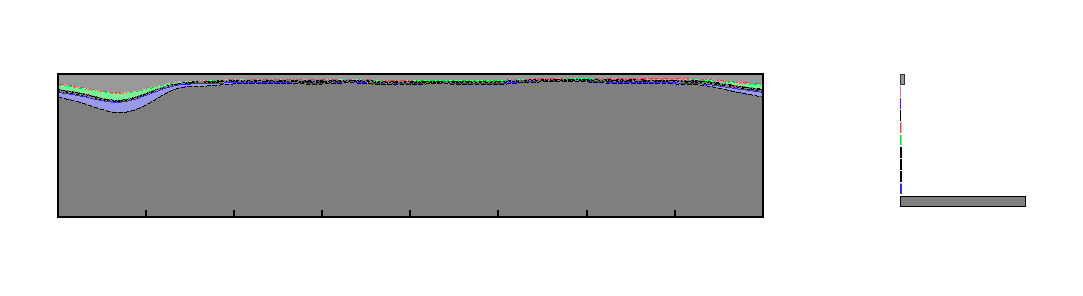
\includegraphics{img/hr-tr}}%
    \gplfronttext
  \end{picture}%
\endgroup


\noindent% GNUPLOT: LaTeX picture with Postscript
\begingroup
  \makeatletter
  \providecommand\color[2][]{%
    \GenericError{(gnuplot) \space\space\space\@spaces}{%
      Package color not loaded in conjunction with
      terminal option `colourtext'%
    }{See the gnuplot documentation for explanation.%
    }{Either use 'blacktext' in gnuplot or load the package
      color.sty in LaTeX.}%
    \renewcommand\color[2][]{}%
  }%
  \providecommand\includegraphics[2][]{%
    \GenericError{(gnuplot) \space\space\space\@spaces}{%
      Package graphicx or graphics not loaded%
    }{See the gnuplot documentation for explanation.%
    }{The gnuplot epslatex terminal needs graphicx.sty or graphics.sty.}%
    \renewcommand\includegraphics[2][]{}%
  }%
  \providecommand\rotatebox[2]{#2}%
  \@ifundefined{ifGPcolor}{%
    \newif\ifGPcolor
    \GPcolorfalse
  }{}%
  \@ifundefined{ifGPblacktext}{%
    \newif\ifGPblacktext
    \GPblacktexttrue
  }{}%
  % define a \g@addto@macro without @ in the name:
  \let\gplgaddtomacro\g@addto@macro
  % define empty templates for all commands taking text:
  \gdef\gplbacktext{}%
  \gdef\gplfronttext{}%
  \makeatother
  \ifGPblacktext
    % no textcolor at all
    \def\colorrgb#1{}%
    \def\colorgray#1{}%
  \else
    % gray or color?
    \ifGPcolor
      \def\colorrgb#1{\color[rgb]{#1}}%
      \def\colorgray#1{\color[gray]{#1}}%
      \expandafter\def\csname LTw\endcsname{\color{white}}%
      \expandafter\def\csname LTb\endcsname{\color{black}}%
      \expandafter\def\csname LTa\endcsname{\color{black}}%
      \expandafter\def\csname LT0\endcsname{\color[rgb]{1,0,0}}%
      \expandafter\def\csname LT1\endcsname{\color[rgb]{0,1,0}}%
      \expandafter\def\csname LT2\endcsname{\color[rgb]{0,0,1}}%
      \expandafter\def\csname LT3\endcsname{\color[rgb]{1,0,1}}%
      \expandafter\def\csname LT4\endcsname{\color[rgb]{0,1,1}}%
      \expandafter\def\csname LT5\endcsname{\color[rgb]{1,1,0}}%
      \expandafter\def\csname LT6\endcsname{\color[rgb]{0,0,0}}%
      \expandafter\def\csname LT7\endcsname{\color[rgb]{1,0.3,0}}%
      \expandafter\def\csname LT8\endcsname{\color[rgb]{0.5,0.5,0.5}}%
    \else
      % gray
      \def\colorrgb#1{\color{black}}%
      \def\colorgray#1{\color[gray]{#1}}%
      \expandafter\def\csname LTw\endcsname{\color{white}}%
      \expandafter\def\csname LTb\endcsname{\color{black}}%
      \expandafter\def\csname LTa\endcsname{\color{black}}%
      \expandafter\def\csname LT0\endcsname{\color{black}}%
      \expandafter\def\csname LT1\endcsname{\color{black}}%
      \expandafter\def\csname LT2\endcsname{\color{black}}%
      \expandafter\def\csname LT3\endcsname{\color{black}}%
      \expandafter\def\csname LT4\endcsname{\color{black}}%
      \expandafter\def\csname LT5\endcsname{\color{black}}%
      \expandafter\def\csname LT6\endcsname{\color{black}}%
      \expandafter\def\csname LT7\endcsname{\color{black}}%
      \expandafter\def\csname LT8\endcsname{\color{black}}%
    \fi
  \fi
  \setlength{\unitlength}{0.0500bp}%
  \begin{picture}(10080.00,2520.00)%
    \gplgaddtomacro\gplbacktext{%
      \csname LTb\endcsname%
      \put(176,1281){\rotatebox{-270}{\makebox(0,0){\strut{}\scriptsize fraction of tweets}}}%
      \put(3779,154){\makebox(0,0){\strut{}\scriptsize time of day (UTC)}}%
      \put(3779,2189){\makebox(0,0){\strut{}Countries that Tweet in Japanese}}%
    }%
    \gplgaddtomacro\gplfronttext{%
      \csname LTb\endcsname%
      \put(396,374){\makebox(0,0){\strut{}\scriptsize 0:00}}%
      \put(1242,374){\makebox(0,0){\strut{}\scriptsize 3:00}}%
      \put(2088,374){\makebox(0,0){\strut{}\scriptsize 6:00}}%
      \put(2934,374){\makebox(0,0){\strut{}\scriptsize 9:00}}%
      \put(3780,374){\makebox(0,0){\strut{}\scriptsize 12:00}}%
      \put(4625,374){\makebox(0,0){\strut{}\scriptsize 15:00}}%
      \put(5471,374){\makebox(0,0){\strut{}\scriptsize 18:00}}%
      \put(6317,374){\makebox(0,0){\strut{}\scriptsize 21:00}}%
      \put(7163,374){\makebox(0,0){\strut{}\scriptsize 24:00}}%
    }%
    \gplgaddtomacro\gplbacktext{%
      \csname LTb\endcsname%
      \put(9083,154){\makebox(0,0){\strut{}~~}}%
      \put(9083,2189){\makebox(0,0){\strut{} }}%
    }%
    \gplgaddtomacro\gplfronttext{%
      \csname LTb\endcsname%
      \put(8352,751){\makebox(0,0)[r]{\strut{}\scriptsize~Japan}}%
      \put(8352,868){\makebox(0,0)[r]{\strut{}\scriptsize~USA}}%
      \put(8352,985){\makebox(0,0)[r]{\strut{}\scriptsize~Taiwan}}%
      \put(8352,1102){\makebox(0,0)[r]{\strut{}\scriptsize~China}}%
      \put(8352,1219){\makebox(0,0)[r]{\strut{}\scriptsize~South~Korea}}%
      \put(8352,1337){\makebox(0,0)[r]{\strut{}\scriptsize~Thailand}}%
      \put(8352,1454){\makebox(0,0)[r]{\strut{}\scriptsize~Hong~Kong}}%
      \put(8352,1571){\makebox(0,0)[r]{\strut{}\scriptsize~Australia}}%
      \put(8352,1688){\makebox(0,0)[r]{\strut{}\scriptsize~Canada}}%
      \put(8352,1805){\makebox(0,0)[r]{\strut{}\scriptsize~Malasia}}%
      \put(8352,1922){\makebox(0,0)[r]{\strut{}\scriptsize~other}}%
    }%
    \gplbacktext
    \put(0,0){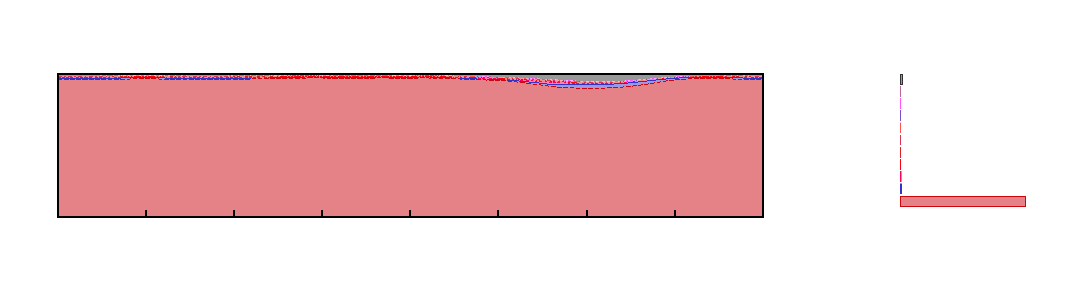
\includegraphics{img/hr-ja}}%
    \gplfronttext
  \end{picture}%
\endgroup


\noindent% GNUPLOT: LaTeX picture with Postscript
\begingroup
  \makeatletter
  \providecommand\color[2][]{%
    \GenericError{(gnuplot) \space\space\space\@spaces}{%
      Package color not loaded in conjunction with
      terminal option `colourtext'%
    }{See the gnuplot documentation for explanation.%
    }{Either use 'blacktext' in gnuplot or load the package
      color.sty in LaTeX.}%
    \renewcommand\color[2][]{}%
  }%
  \providecommand\includegraphics[2][]{%
    \GenericError{(gnuplot) \space\space\space\@spaces}{%
      Package graphicx or graphics not loaded%
    }{See the gnuplot documentation for explanation.%
    }{The gnuplot epslatex terminal needs graphicx.sty or graphics.sty.}%
    \renewcommand\includegraphics[2][]{}%
  }%
  \providecommand\rotatebox[2]{#2}%
  \@ifundefined{ifGPcolor}{%
    \newif\ifGPcolor
    \GPcolorfalse
  }{}%
  \@ifundefined{ifGPblacktext}{%
    \newif\ifGPblacktext
    \GPblacktexttrue
  }{}%
  % define a \g@addto@macro without @ in the name:
  \let\gplgaddtomacro\g@addto@macro
  % define empty templates for all commands taking text:
  \gdef\gplbacktext{}%
  \gdef\gplfronttext{}%
  \makeatother
  \ifGPblacktext
    % no textcolor at all
    \def\colorrgb#1{}%
    \def\colorgray#1{}%
  \else
    % gray or color?
    \ifGPcolor
      \def\colorrgb#1{\color[rgb]{#1}}%
      \def\colorgray#1{\color[gray]{#1}}%
      \expandafter\def\csname LTw\endcsname{\color{white}}%
      \expandafter\def\csname LTb\endcsname{\color{black}}%
      \expandafter\def\csname LTa\endcsname{\color{black}}%
      \expandafter\def\csname LT0\endcsname{\color[rgb]{1,0,0}}%
      \expandafter\def\csname LT1\endcsname{\color[rgb]{0,1,0}}%
      \expandafter\def\csname LT2\endcsname{\color[rgb]{0,0,1}}%
      \expandafter\def\csname LT3\endcsname{\color[rgb]{1,0,1}}%
      \expandafter\def\csname LT4\endcsname{\color[rgb]{0,1,1}}%
      \expandafter\def\csname LT5\endcsname{\color[rgb]{1,1,0}}%
      \expandafter\def\csname LT6\endcsname{\color[rgb]{0,0,0}}%
      \expandafter\def\csname LT7\endcsname{\color[rgb]{1,0.3,0}}%
      \expandafter\def\csname LT8\endcsname{\color[rgb]{0.5,0.5,0.5}}%
    \else
      % gray
      \def\colorrgb#1{\color{black}}%
      \def\colorgray#1{\color[gray]{#1}}%
      \expandafter\def\csname LTw\endcsname{\color{white}}%
      \expandafter\def\csname LTb\endcsname{\color{black}}%
      \expandafter\def\csname LTa\endcsname{\color{black}}%
      \expandafter\def\csname LT0\endcsname{\color{black}}%
      \expandafter\def\csname LT1\endcsname{\color{black}}%
      \expandafter\def\csname LT2\endcsname{\color{black}}%
      \expandafter\def\csname LT3\endcsname{\color{black}}%
      \expandafter\def\csname LT4\endcsname{\color{black}}%
      \expandafter\def\csname LT5\endcsname{\color{black}}%
      \expandafter\def\csname LT6\endcsname{\color{black}}%
      \expandafter\def\csname LT7\endcsname{\color{black}}%
      \expandafter\def\csname LT8\endcsname{\color{black}}%
    \fi
  \fi
  \setlength{\unitlength}{0.0500bp}%
  \begin{picture}(10080.00,2520.00)%
    \gplgaddtomacro\gplbacktext{%
      \csname LTb\endcsname%
      \put(176,1281){\rotatebox{-270}{\makebox(0,0){\strut{}\scriptsize fraction of tweets}}}%
      \put(3779,154){\makebox(0,0){\strut{}\scriptsize time of day (UTC)}}%
      \put(3779,2189){\makebox(0,0){\strut{}Countries that Tweet in Korean}}%
    }%
    \gplgaddtomacro\gplfronttext{%
      \csname LTb\endcsname%
      \put(396,374){\makebox(0,0){\strut{}\scriptsize 0:00}}%
      \put(1242,374){\makebox(0,0){\strut{}\scriptsize 3:00}}%
      \put(2088,374){\makebox(0,0){\strut{}\scriptsize 6:00}}%
      \put(2934,374){\makebox(0,0){\strut{}\scriptsize 9:00}}%
      \put(3780,374){\makebox(0,0){\strut{}\scriptsize 12:00}}%
      \put(4625,374){\makebox(0,0){\strut{}\scriptsize 15:00}}%
      \put(5471,374){\makebox(0,0){\strut{}\scriptsize 18:00}}%
      \put(6317,374){\makebox(0,0){\strut{}\scriptsize 21:00}}%
      \put(7163,374){\makebox(0,0){\strut{}\scriptsize 24:00}}%
    }%
    \gplgaddtomacro\gplbacktext{%
      \csname LTb\endcsname%
      \put(9083,154){\makebox(0,0){\strut{}~~}}%
      \put(9083,2189){\makebox(0,0){\strut{} }}%
    }%
    \gplgaddtomacro\gplfronttext{%
      \csname LTb\endcsname%
      \put(8352,751){\makebox(0,0)[r]{\strut{}\scriptsize~South~Korea}}%
      \put(8352,868){\makebox(0,0)[r]{\strut{}\scriptsize~Japan}}%
      \put(8352,985){\makebox(0,0)[r]{\strut{}\scriptsize~USA}}%
      \put(8352,1102){\makebox(0,0)[r]{\strut{}\scriptsize~Thailand}}%
      \put(8352,1219){\makebox(0,0)[r]{\strut{}\scriptsize~Philippines}}%
      \put(8352,1337){\makebox(0,0)[r]{\strut{}\scriptsize~Canada}}%
      \put(8352,1454){\makebox(0,0)[r]{\strut{}\scriptsize~Indonesia}}%
      \put(8352,1571){\makebox(0,0)[r]{\strut{}\scriptsize~DE}}%
      \put(8352,1688){\makebox(0,0)[r]{\strut{}\scriptsize~Brazil}}%
      \put(8352,1805){\makebox(0,0)[r]{\strut{}\scriptsize~Malasia}}%
      \put(8352,1922){\makebox(0,0)[r]{\strut{}\scriptsize~other}}%
    }%
    \gplbacktext
    \put(0,0){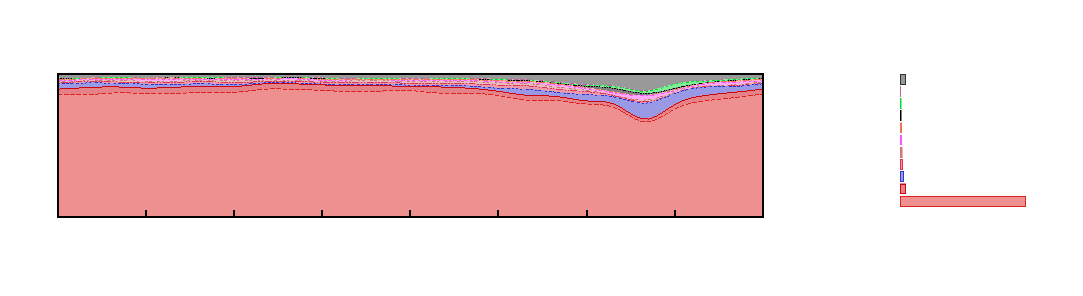
\includegraphics{img/hr-ko}}%
    \gplfronttext
  \end{picture}%
\endgroup


\noindent% GNUPLOT: LaTeX picture with Postscript
\begingroup
  \makeatletter
  \providecommand\color[2][]{%
    \GenericError{(gnuplot) \space\space\space\@spaces}{%
      Package color not loaded in conjunction with
      terminal option `colourtext'%
    }{See the gnuplot documentation for explanation.%
    }{Either use 'blacktext' in gnuplot or load the package
      color.sty in LaTeX.}%
    \renewcommand\color[2][]{}%
  }%
  \providecommand\includegraphics[2][]{%
    \GenericError{(gnuplot) \space\space\space\@spaces}{%
      Package graphicx or graphics not loaded%
    }{See the gnuplot documentation for explanation.%
    }{The gnuplot epslatex terminal needs graphicx.sty or graphics.sty.}%
    \renewcommand\includegraphics[2][]{}%
  }%
  \providecommand\rotatebox[2]{#2}%
  \@ifundefined{ifGPcolor}{%
    \newif\ifGPcolor
    \GPcolorfalse
  }{}%
  \@ifundefined{ifGPblacktext}{%
    \newif\ifGPblacktext
    \GPblacktexttrue
  }{}%
  % define a \g@addto@macro without @ in the name:
  \let\gplgaddtomacro\g@addto@macro
  % define empty templates for all commands taking text:
  \gdef\gplbacktext{}%
  \gdef\gplfronttext{}%
  \makeatother
  \ifGPblacktext
    % no textcolor at all
    \def\colorrgb#1{}%
    \def\colorgray#1{}%
  \else
    % gray or color?
    \ifGPcolor
      \def\colorrgb#1{\color[rgb]{#1}}%
      \def\colorgray#1{\color[gray]{#1}}%
      \expandafter\def\csname LTw\endcsname{\color{white}}%
      \expandafter\def\csname LTb\endcsname{\color{black}}%
      \expandafter\def\csname LTa\endcsname{\color{black}}%
      \expandafter\def\csname LT0\endcsname{\color[rgb]{1,0,0}}%
      \expandafter\def\csname LT1\endcsname{\color[rgb]{0,1,0}}%
      \expandafter\def\csname LT2\endcsname{\color[rgb]{0,0,1}}%
      \expandafter\def\csname LT3\endcsname{\color[rgb]{1,0,1}}%
      \expandafter\def\csname LT4\endcsname{\color[rgb]{0,1,1}}%
      \expandafter\def\csname LT5\endcsname{\color[rgb]{1,1,0}}%
      \expandafter\def\csname LT6\endcsname{\color[rgb]{0,0,0}}%
      \expandafter\def\csname LT7\endcsname{\color[rgb]{1,0.3,0}}%
      \expandafter\def\csname LT8\endcsname{\color[rgb]{0.5,0.5,0.5}}%
    \else
      % gray
      \def\colorrgb#1{\color{black}}%
      \def\colorgray#1{\color[gray]{#1}}%
      \expandafter\def\csname LTw\endcsname{\color{white}}%
      \expandafter\def\csname LTb\endcsname{\color{black}}%
      \expandafter\def\csname LTa\endcsname{\color{black}}%
      \expandafter\def\csname LT0\endcsname{\color{black}}%
      \expandafter\def\csname LT1\endcsname{\color{black}}%
      \expandafter\def\csname LT2\endcsname{\color{black}}%
      \expandafter\def\csname LT3\endcsname{\color{black}}%
      \expandafter\def\csname LT4\endcsname{\color{black}}%
      \expandafter\def\csname LT5\endcsname{\color{black}}%
      \expandafter\def\csname LT6\endcsname{\color{black}}%
      \expandafter\def\csname LT7\endcsname{\color{black}}%
      \expandafter\def\csname LT8\endcsname{\color{black}}%
    \fi
  \fi
  \setlength{\unitlength}{0.0500bp}%
  \begin{picture}(10080.00,2520.00)%
    \gplgaddtomacro\gplbacktext{%
      \csname LTb\endcsname%
      \put(176,1281){\rotatebox{-270}{\makebox(0,0){\strut{}\scriptsize fraction of tweets}}}%
      \put(3779,154){\makebox(0,0){\strut{}\scriptsize time of day (UTC)}}%
      \put(3779,2189){\makebox(0,0){\strut{}Countries that Tweet in Portuguese}}%
    }%
    \gplgaddtomacro\gplfronttext{%
      \csname LTb\endcsname%
      \put(396,374){\makebox(0,0){\strut{}\scriptsize 0:00}}%
      \put(1242,374){\makebox(0,0){\strut{}\scriptsize 3:00}}%
      \put(2088,374){\makebox(0,0){\strut{}\scriptsize 6:00}}%
      \put(2934,374){\makebox(0,0){\strut{}\scriptsize 9:00}}%
      \put(3780,374){\makebox(0,0){\strut{}\scriptsize 12:00}}%
      \put(4625,374){\makebox(0,0){\strut{}\scriptsize 15:00}}%
      \put(5471,374){\makebox(0,0){\strut{}\scriptsize 18:00}}%
      \put(6317,374){\makebox(0,0){\strut{}\scriptsize 21:00}}%
      \put(7163,374){\makebox(0,0){\strut{}\scriptsize 24:00}}%
    }%
    \gplgaddtomacro\gplbacktext{%
      \csname LTb\endcsname%
      \put(9083,154){\makebox(0,0){\strut{}~~}}%
      \put(9083,2189){\makebox(0,0){\strut{} }}%
    }%
    \gplgaddtomacro\gplfronttext{%
      \csname LTb\endcsname%
      \put(8352,751){\makebox(0,0)[r]{\strut{}\scriptsize~Brazil}}%
      \put(8352,868){\makebox(0,0)[r]{\strut{}\scriptsize~Portugal}}%
      \put(8352,985){\makebox(0,0)[r]{\strut{}\scriptsize~USA}}%
      \put(8352,1102){\makebox(0,0)[r]{\strut{}\scriptsize~Argentina}}%
      \put(8352,1219){\makebox(0,0)[r]{\strut{}\scriptsize~Spain}}%
      \put(8352,1337){\makebox(0,0)[r]{\strut{}\scriptsize~Mexico}}%
      \put(8352,1454){\makebox(0,0)[r]{\strut{}\scriptsize~UK}}%
      \put(8352,1571){\makebox(0,0)[r]{\strut{}\scriptsize~France}}%
      \put(8352,1688){\makebox(0,0)[r]{\strut{}\scriptsize~Italy}}%
      \put(8352,1805){\makebox(0,0)[r]{\strut{}\scriptsize~Uruguay}}%
      \put(8352,1922){\makebox(0,0)[r]{\strut{}\scriptsize~other}}%
    }%
    \gplbacktext
    \put(0,0){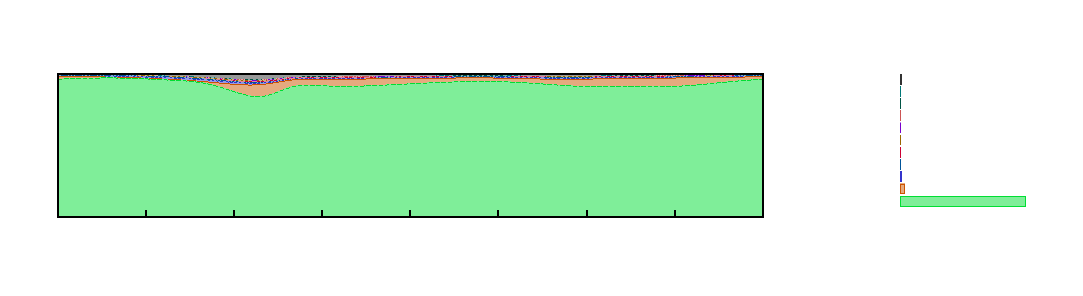
\includegraphics{img/hr-pt}}%
    \gplfronttext
  \end{picture}%
\endgroup


\noindent% GNUPLOT: LaTeX picture with Postscript
\begingroup
  \makeatletter
  \providecommand\color[2][]{%
    \GenericError{(gnuplot) \space\space\space\@spaces}{%
      Package color not loaded in conjunction with
      terminal option `colourtext'%
    }{See the gnuplot documentation for explanation.%
    }{Either use 'blacktext' in gnuplot or load the package
      color.sty in LaTeX.}%
    \renewcommand\color[2][]{}%
  }%
  \providecommand\includegraphics[2][]{%
    \GenericError{(gnuplot) \space\space\space\@spaces}{%
      Package graphicx or graphics not loaded%
    }{See the gnuplot documentation for explanation.%
    }{The gnuplot epslatex terminal needs graphicx.sty or graphics.sty.}%
    \renewcommand\includegraphics[2][]{}%
  }%
  \providecommand\rotatebox[2]{#2}%
  \@ifundefined{ifGPcolor}{%
    \newif\ifGPcolor
    \GPcolorfalse
  }{}%
  \@ifundefined{ifGPblacktext}{%
    \newif\ifGPblacktext
    \GPblacktexttrue
  }{}%
  % define a \g@addto@macro without @ in the name:
  \let\gplgaddtomacro\g@addto@macro
  % define empty templates for all commands taking text:
  \gdef\gplbacktext{}%
  \gdef\gplfronttext{}%
  \makeatother
  \ifGPblacktext
    % no textcolor at all
    \def\colorrgb#1{}%
    \def\colorgray#1{}%
  \else
    % gray or color?
    \ifGPcolor
      \def\colorrgb#1{\color[rgb]{#1}}%
      \def\colorgray#1{\color[gray]{#1}}%
      \expandafter\def\csname LTw\endcsname{\color{white}}%
      \expandafter\def\csname LTb\endcsname{\color{black}}%
      \expandafter\def\csname LTa\endcsname{\color{black}}%
      \expandafter\def\csname LT0\endcsname{\color[rgb]{1,0,0}}%
      \expandafter\def\csname LT1\endcsname{\color[rgb]{0,1,0}}%
      \expandafter\def\csname LT2\endcsname{\color[rgb]{0,0,1}}%
      \expandafter\def\csname LT3\endcsname{\color[rgb]{1,0,1}}%
      \expandafter\def\csname LT4\endcsname{\color[rgb]{0,1,1}}%
      \expandafter\def\csname LT5\endcsname{\color[rgb]{1,1,0}}%
      \expandafter\def\csname LT6\endcsname{\color[rgb]{0,0,0}}%
      \expandafter\def\csname LT7\endcsname{\color[rgb]{1,0.3,0}}%
      \expandafter\def\csname LT8\endcsname{\color[rgb]{0.5,0.5,0.5}}%
    \else
      % gray
      \def\colorrgb#1{\color{black}}%
      \def\colorgray#1{\color[gray]{#1}}%
      \expandafter\def\csname LTw\endcsname{\color{white}}%
      \expandafter\def\csname LTb\endcsname{\color{black}}%
      \expandafter\def\csname LTa\endcsname{\color{black}}%
      \expandafter\def\csname LT0\endcsname{\color{black}}%
      \expandafter\def\csname LT1\endcsname{\color{black}}%
      \expandafter\def\csname LT2\endcsname{\color{black}}%
      \expandafter\def\csname LT3\endcsname{\color{black}}%
      \expandafter\def\csname LT4\endcsname{\color{black}}%
      \expandafter\def\csname LT5\endcsname{\color{black}}%
      \expandafter\def\csname LT6\endcsname{\color{black}}%
      \expandafter\def\csname LT7\endcsname{\color{black}}%
      \expandafter\def\csname LT8\endcsname{\color{black}}%
    \fi
  \fi
  \setlength{\unitlength}{0.0500bp}%
  \begin{picture}(10080.00,2520.00)%
    \gplgaddtomacro\gplbacktext{%
      \csname LTb\endcsname%
      \put(176,1281){\rotatebox{-270}{\makebox(0,0){\strut{}\scriptsize fraction of tweets}}}%
      \put(3779,154){\makebox(0,0){\strut{}\scriptsize time of day (UTC)}}%
      \put(3779,2189){\makebox(0,0){\strut{}Countries that Tweet in Chinese}}%
    }%
    \gplgaddtomacro\gplfronttext{%
      \csname LTb\endcsname%
      \put(396,374){\makebox(0,0){\strut{}\scriptsize 0:00}}%
      \put(1242,374){\makebox(0,0){\strut{}\scriptsize 3:00}}%
      \put(2088,374){\makebox(0,0){\strut{}\scriptsize 6:00}}%
      \put(2934,374){\makebox(0,0){\strut{}\scriptsize 9:00}}%
      \put(3780,374){\makebox(0,0){\strut{}\scriptsize 12:00}}%
      \put(4625,374){\makebox(0,0){\strut{}\scriptsize 15:00}}%
      \put(5471,374){\makebox(0,0){\strut{}\scriptsize 18:00}}%
      \put(6317,374){\makebox(0,0){\strut{}\scriptsize 21:00}}%
      \put(7163,374){\makebox(0,0){\strut{}\scriptsize 24:00}}%
    }%
    \gplgaddtomacro\gplbacktext{%
      \csname LTb\endcsname%
      \put(9083,154){\makebox(0,0){\strut{}~~}}%
      \put(9083,2189){\makebox(0,0){\strut{} }}%
    }%
    \gplgaddtomacro\gplfronttext{%
      \csname LTb\endcsname%
      \put(8352,751){\makebox(0,0)[r]{\strut{}\scriptsize~China}}%
      \put(8352,868){\makebox(0,0)[r]{\strut{}\scriptsize~Taiwan}}%
      \put(8352,985){\makebox(0,0)[r]{\strut{}\scriptsize~USA}}%
      \put(8352,1102){\makebox(0,0)[r]{\strut{}\scriptsize~Japan}}%
      \put(8352,1219){\makebox(0,0)[r]{\strut{}\scriptsize~Malasia}}%
      \put(8352,1337){\makebox(0,0)[r]{\strut{}\scriptsize~Hong~Kong}}%
      \put(8352,1454){\makebox(0,0)[r]{\strut{}\scriptsize~Canada}}%
      \put(8352,1571){\makebox(0,0)[r]{\strut{}\scriptsize~Australia}}%
      \put(8352,1688){\makebox(0,0)[r]{\strut{}\scriptsize~Singapore}}%
      \put(8352,1805){\makebox(0,0)[r]{\strut{}\scriptsize~UK}}%
      \put(8352,1922){\makebox(0,0)[r]{\strut{}\scriptsize~other}}%
    }%
    \gplbacktext
    \put(0,0){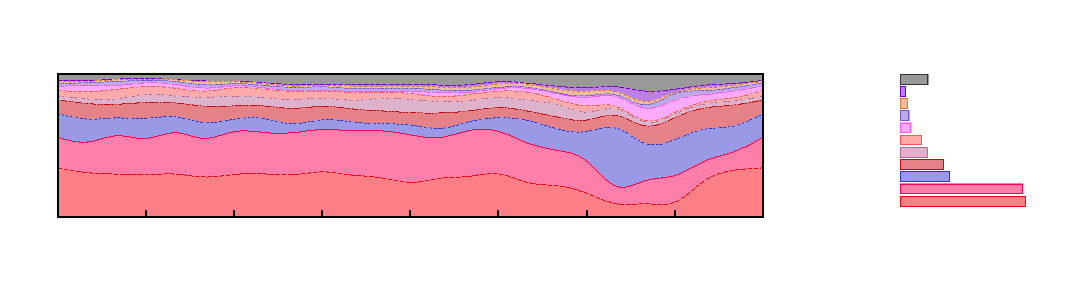
\includegraphics{img/hr-zh}}%
    \gplfronttext
  \end{picture}%
\endgroup


\noindent% GNUPLOT: LaTeX picture with Postscript
\begingroup
  \makeatletter
  \providecommand\color[2][]{%
    \GenericError{(gnuplot) \space\space\space\@spaces}{%
      Package color not loaded in conjunction with
      terminal option `colourtext'%
    }{See the gnuplot documentation for explanation.%
    }{Either use 'blacktext' in gnuplot or load the package
      color.sty in LaTeX.}%
    \renewcommand\color[2][]{}%
  }%
  \providecommand\includegraphics[2][]{%
    \GenericError{(gnuplot) \space\space\space\@spaces}{%
      Package graphicx or graphics not loaded%
    }{See the gnuplot documentation for explanation.%
    }{The gnuplot epslatex terminal needs graphicx.sty or graphics.sty.}%
    \renewcommand\includegraphics[2][]{}%
  }%
  \providecommand\rotatebox[2]{#2}%
  \@ifundefined{ifGPcolor}{%
    \newif\ifGPcolor
    \GPcolorfalse
  }{}%
  \@ifundefined{ifGPblacktext}{%
    \newif\ifGPblacktext
    \GPblacktexttrue
  }{}%
  % define a \g@addto@macro without @ in the name:
  \let\gplgaddtomacro\g@addto@macro
  % define empty templates for all commands taking text:
  \gdef\gplbacktext{}%
  \gdef\gplfronttext{}%
  \makeatother
  \ifGPblacktext
    % no textcolor at all
    \def\colorrgb#1{}%
    \def\colorgray#1{}%
  \else
    % gray or color?
    \ifGPcolor
      \def\colorrgb#1{\color[rgb]{#1}}%
      \def\colorgray#1{\color[gray]{#1}}%
      \expandafter\def\csname LTw\endcsname{\color{white}}%
      \expandafter\def\csname LTb\endcsname{\color{black}}%
      \expandafter\def\csname LTa\endcsname{\color{black}}%
      \expandafter\def\csname LT0\endcsname{\color[rgb]{1,0,0}}%
      \expandafter\def\csname LT1\endcsname{\color[rgb]{0,1,0}}%
      \expandafter\def\csname LT2\endcsname{\color[rgb]{0,0,1}}%
      \expandafter\def\csname LT3\endcsname{\color[rgb]{1,0,1}}%
      \expandafter\def\csname LT4\endcsname{\color[rgb]{0,1,1}}%
      \expandafter\def\csname LT5\endcsname{\color[rgb]{1,1,0}}%
      \expandafter\def\csname LT6\endcsname{\color[rgb]{0,0,0}}%
      \expandafter\def\csname LT7\endcsname{\color[rgb]{1,0.3,0}}%
      \expandafter\def\csname LT8\endcsname{\color[rgb]{0.5,0.5,0.5}}%
    \else
      % gray
      \def\colorrgb#1{\color{black}}%
      \def\colorgray#1{\color[gray]{#1}}%
      \expandafter\def\csname LTw\endcsname{\color{white}}%
      \expandafter\def\csname LTb\endcsname{\color{black}}%
      \expandafter\def\csname LTa\endcsname{\color{black}}%
      \expandafter\def\csname LT0\endcsname{\color{black}}%
      \expandafter\def\csname LT1\endcsname{\color{black}}%
      \expandafter\def\csname LT2\endcsname{\color{black}}%
      \expandafter\def\csname LT3\endcsname{\color{black}}%
      \expandafter\def\csname LT4\endcsname{\color{black}}%
      \expandafter\def\csname LT5\endcsname{\color{black}}%
      \expandafter\def\csname LT6\endcsname{\color{black}}%
      \expandafter\def\csname LT7\endcsname{\color{black}}%
      \expandafter\def\csname LT8\endcsname{\color{black}}%
    \fi
  \fi
  \setlength{\unitlength}{0.0500bp}%
  \begin{picture}(10080.00,2520.00)%
    \gplgaddtomacro\gplbacktext{%
      \csname LTb\endcsname%
      \put(176,1281){\rotatebox{-270}{\makebox(0,0){\strut{}\scriptsize fraction of tweets}}}%
      \put(3779,154){\makebox(0,0){\strut{}\scriptsize time of day (UTC)}}%
      \put(3779,2189){\makebox(0,0){\strut{}Countries that Tweet in und}}%
    }%
    \gplgaddtomacro\gplfronttext{%
      \csname LTb\endcsname%
      \put(396,374){\makebox(0,0){\strut{}\scriptsize 0:00}}%
      \put(1242,374){\makebox(0,0){\strut{}\scriptsize 3:00}}%
      \put(2088,374){\makebox(0,0){\strut{}\scriptsize 6:00}}%
      \put(2934,374){\makebox(0,0){\strut{}\scriptsize 9:00}}%
      \put(3780,374){\makebox(0,0){\strut{}\scriptsize 12:00}}%
      \put(4625,374){\makebox(0,0){\strut{}\scriptsize 15:00}}%
      \put(5471,374){\makebox(0,0){\strut{}\scriptsize 18:00}}%
      \put(6317,374){\makebox(0,0){\strut{}\scriptsize 21:00}}%
      \put(7163,374){\makebox(0,0){\strut{}\scriptsize 24:00}}%
    }%
    \gplgaddtomacro\gplbacktext{%
      \csname LTb\endcsname%
      \put(9083,154){\makebox(0,0){\strut{}~~}}%
      \put(9083,2189){\makebox(0,0){\strut{} }}%
    }%
    \gplgaddtomacro\gplfronttext{%
      \csname LTb\endcsname%
      \put(8352,751){\makebox(0,0)[r]{\strut{}\scriptsize~USA}}%
      \put(8352,868){\makebox(0,0)[r]{\strut{}\scriptsize~Brazil}}%
      \put(8352,985){\makebox(0,0)[r]{\strut{}\scriptsize~Spain}}%
      \put(8352,1102){\makebox(0,0)[r]{\strut{}\scriptsize~UK}}%
      \put(8352,1219){\makebox(0,0)[r]{\strut{}\scriptsize~Philippines}}%
      \put(8352,1337){\makebox(0,0)[r]{\strut{}\scriptsize~India}}%
      \put(8352,1454){\makebox(0,0)[r]{\strut{}\scriptsize~TR}}%
      \put(8352,1571){\makebox(0,0)[r]{\strut{}\scriptsize~France}}%
      \put(8352,1688){\makebox(0,0)[r]{\strut{}\scriptsize~Saudi~Arabia}}%
      \put(8352,1805){\makebox(0,0)[r]{\strut{}\scriptsize~Argentina}}%
      \put(8352,1922){\makebox(0,0)[r]{\strut{}\scriptsize~other}}%
    }%
    \gplbacktext
    \put(0,0){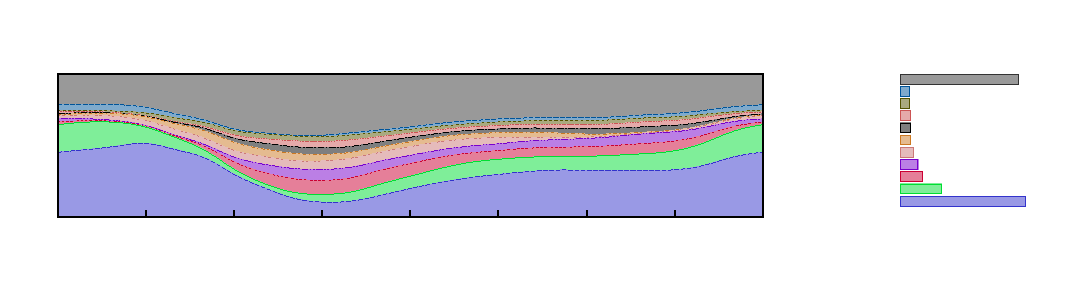
\includegraphics{img/hr-und}}%
    \gplfronttext
  \end{picture}%
\endgroup


\noindent% GNUPLOT: LaTeX picture with Postscript
\begingroup
  \makeatletter
  \providecommand\color[2][]{%
    \GenericError{(gnuplot) \space\space\space\@spaces}{%
      Package color not loaded in conjunction with
      terminal option `colourtext'%
    }{See the gnuplot documentation for explanation.%
    }{Either use 'blacktext' in gnuplot or load the package
      color.sty in LaTeX.}%
    \renewcommand\color[2][]{}%
  }%
  \providecommand\includegraphics[2][]{%
    \GenericError{(gnuplot) \space\space\space\@spaces}{%
      Package graphicx or graphics not loaded%
    }{See the gnuplot documentation for explanation.%
    }{The gnuplot epslatex terminal needs graphicx.sty or graphics.sty.}%
    \renewcommand\includegraphics[2][]{}%
  }%
  \providecommand\rotatebox[2]{#2}%
  \@ifundefined{ifGPcolor}{%
    \newif\ifGPcolor
    \GPcolorfalse
  }{}%
  \@ifundefined{ifGPblacktext}{%
    \newif\ifGPblacktext
    \GPblacktexttrue
  }{}%
  % define a \g@addto@macro without @ in the name:
  \let\gplgaddtomacro\g@addto@macro
  % define empty templates for all commands taking text:
  \gdef\gplbacktext{}%
  \gdef\gplfronttext{}%
  \makeatother
  \ifGPblacktext
    % no textcolor at all
    \def\colorrgb#1{}%
    \def\colorgray#1{}%
  \else
    % gray or color?
    \ifGPcolor
      \def\colorrgb#1{\color[rgb]{#1}}%
      \def\colorgray#1{\color[gray]{#1}}%
      \expandafter\def\csname LTw\endcsname{\color{white}}%
      \expandafter\def\csname LTb\endcsname{\color{black}}%
      \expandafter\def\csname LTa\endcsname{\color{black}}%
      \expandafter\def\csname LT0\endcsname{\color[rgb]{1,0,0}}%
      \expandafter\def\csname LT1\endcsname{\color[rgb]{0,1,0}}%
      \expandafter\def\csname LT2\endcsname{\color[rgb]{0,0,1}}%
      \expandafter\def\csname LT3\endcsname{\color[rgb]{1,0,1}}%
      \expandafter\def\csname LT4\endcsname{\color[rgb]{0,1,1}}%
      \expandafter\def\csname LT5\endcsname{\color[rgb]{1,1,0}}%
      \expandafter\def\csname LT6\endcsname{\color[rgb]{0,0,0}}%
      \expandafter\def\csname LT7\endcsname{\color[rgb]{1,0.3,0}}%
      \expandafter\def\csname LT8\endcsname{\color[rgb]{0.5,0.5,0.5}}%
    \else
      % gray
      \def\colorrgb#1{\color{black}}%
      \def\colorgray#1{\color[gray]{#1}}%
      \expandafter\def\csname LTw\endcsname{\color{white}}%
      \expandafter\def\csname LTb\endcsname{\color{black}}%
      \expandafter\def\csname LTa\endcsname{\color{black}}%
      \expandafter\def\csname LT0\endcsname{\color{black}}%
      \expandafter\def\csname LT1\endcsname{\color{black}}%
      \expandafter\def\csname LT2\endcsname{\color{black}}%
      \expandafter\def\csname LT3\endcsname{\color{black}}%
      \expandafter\def\csname LT4\endcsname{\color{black}}%
      \expandafter\def\csname LT5\endcsname{\color{black}}%
      \expandafter\def\csname LT6\endcsname{\color{black}}%
      \expandafter\def\csname LT7\endcsname{\color{black}}%
      \expandafter\def\csname LT8\endcsname{\color{black}}%
    \fi
  \fi
  \setlength{\unitlength}{0.0500bp}%
  \begin{picture}(10080.00,2520.00)%
    \gplgaddtomacro\gplbacktext{%
      \csname LTb\endcsname%
      \put(176,1281){\rotatebox{-270}{\makebox(0,0){\strut{}\scriptsize fraction of tweets}}}%
      \put(3779,154){\makebox(0,0){\strut{}\scriptsize time of day (UTC)}}%
      \put(3779,2189){\makebox(0,0){\strut{}Countries that Tweet in German}}%
    }%
    \gplgaddtomacro\gplfronttext{%
      \csname LTb\endcsname%
      \put(396,374){\makebox(0,0){\strut{}\scriptsize 0:00}}%
      \put(1242,374){\makebox(0,0){\strut{}\scriptsize 3:00}}%
      \put(2088,374){\makebox(0,0){\strut{}\scriptsize 6:00}}%
      \put(2934,374){\makebox(0,0){\strut{}\scriptsize 9:00}}%
      \put(3780,374){\makebox(0,0){\strut{}\scriptsize 12:00}}%
      \put(4625,374){\makebox(0,0){\strut{}\scriptsize 15:00}}%
      \put(5471,374){\makebox(0,0){\strut{}\scriptsize 18:00}}%
      \put(6317,374){\makebox(0,0){\strut{}\scriptsize 21:00}}%
      \put(7163,374){\makebox(0,0){\strut{}\scriptsize 24:00}}%
    }%
    \gplgaddtomacro\gplbacktext{%
      \csname LTb\endcsname%
      \put(9083,154){\makebox(0,0){\strut{}~~}}%
      \put(9083,2189){\makebox(0,0){\strut{} }}%
    }%
    \gplgaddtomacro\gplfronttext{%
      \csname LTb\endcsname%
      \put(8352,751){\makebox(0,0)[r]{\strut{}\scriptsize~DE}}%
      \put(8352,868){\makebox(0,0)[r]{\strut{}\scriptsize~USA}}%
      \put(8352,985){\makebox(0,0)[r]{\strut{}\scriptsize~AT}}%
      \put(8352,1102){\makebox(0,0)[r]{\strut{}\scriptsize~Switzerland}}%
      \put(8352,1219){\makebox(0,0)[r]{\strut{}\scriptsize~DZ}}%
      \put(8352,1337){\makebox(0,0)[r]{\strut{}\scriptsize~Brazil}}%
      \put(8352,1454){\makebox(0,0)[r]{\strut{}\scriptsize~UK}}%
      \put(8352,1571){\makebox(0,0)[r]{\strut{}\scriptsize~Philippines}}%
      \put(8352,1688){\makebox(0,0)[r]{\strut{}\scriptsize~Spain}}%
      \put(8352,1805){\makebox(0,0)[r]{\strut{}\scriptsize~France}}%
      \put(8352,1922){\makebox(0,0)[r]{\strut{}\scriptsize~other}}%
    }%
    \gplbacktext
    \put(0,0){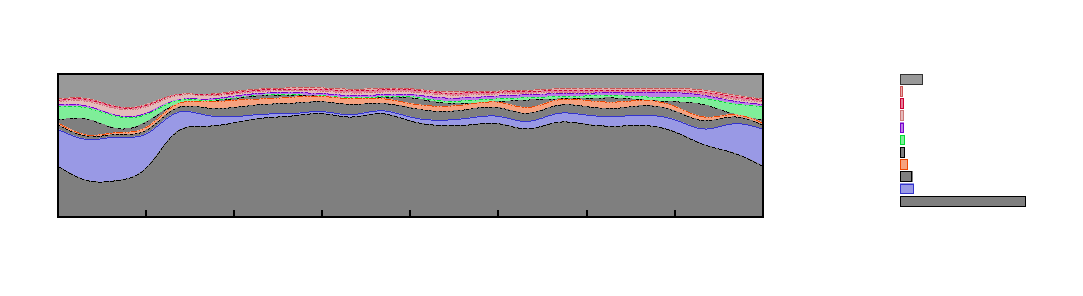
\includegraphics{img/hr-de}}%
    \gplfronttext
  \end{picture}%
\endgroup


\noindent% GNUPLOT: LaTeX picture with Postscript
\begingroup
  \makeatletter
  \providecommand\color[2][]{%
    \GenericError{(gnuplot) \space\space\space\@spaces}{%
      Package color not loaded in conjunction with
      terminal option `colourtext'%
    }{See the gnuplot documentation for explanation.%
    }{Either use 'blacktext' in gnuplot or load the package
      color.sty in LaTeX.}%
    \renewcommand\color[2][]{}%
  }%
  \providecommand\includegraphics[2][]{%
    \GenericError{(gnuplot) \space\space\space\@spaces}{%
      Package graphicx or graphics not loaded%
    }{See the gnuplot documentation for explanation.%
    }{The gnuplot epslatex terminal needs graphicx.sty or graphics.sty.}%
    \renewcommand\includegraphics[2][]{}%
  }%
  \providecommand\rotatebox[2]{#2}%
  \@ifundefined{ifGPcolor}{%
    \newif\ifGPcolor
    \GPcolorfalse
  }{}%
  \@ifundefined{ifGPblacktext}{%
    \newif\ifGPblacktext
    \GPblacktexttrue
  }{}%
  % define a \g@addto@macro without @ in the name:
  \let\gplgaddtomacro\g@addto@macro
  % define empty templates for all commands taking text:
  \gdef\gplbacktext{}%
  \gdef\gplfronttext{}%
  \makeatother
  \ifGPblacktext
    % no textcolor at all
    \def\colorrgb#1{}%
    \def\colorgray#1{}%
  \else
    % gray or color?
    \ifGPcolor
      \def\colorrgb#1{\color[rgb]{#1}}%
      \def\colorgray#1{\color[gray]{#1}}%
      \expandafter\def\csname LTw\endcsname{\color{white}}%
      \expandafter\def\csname LTb\endcsname{\color{black}}%
      \expandafter\def\csname LTa\endcsname{\color{black}}%
      \expandafter\def\csname LT0\endcsname{\color[rgb]{1,0,0}}%
      \expandafter\def\csname LT1\endcsname{\color[rgb]{0,1,0}}%
      \expandafter\def\csname LT2\endcsname{\color[rgb]{0,0,1}}%
      \expandafter\def\csname LT3\endcsname{\color[rgb]{1,0,1}}%
      \expandafter\def\csname LT4\endcsname{\color[rgb]{0,1,1}}%
      \expandafter\def\csname LT5\endcsname{\color[rgb]{1,1,0}}%
      \expandafter\def\csname LT6\endcsname{\color[rgb]{0,0,0}}%
      \expandafter\def\csname LT7\endcsname{\color[rgb]{1,0.3,0}}%
      \expandafter\def\csname LT8\endcsname{\color[rgb]{0.5,0.5,0.5}}%
    \else
      % gray
      \def\colorrgb#1{\color{black}}%
      \def\colorgray#1{\color[gray]{#1}}%
      \expandafter\def\csname LTw\endcsname{\color{white}}%
      \expandafter\def\csname LTb\endcsname{\color{black}}%
      \expandafter\def\csname LTa\endcsname{\color{black}}%
      \expandafter\def\csname LT0\endcsname{\color{black}}%
      \expandafter\def\csname LT1\endcsname{\color{black}}%
      \expandafter\def\csname LT2\endcsname{\color{black}}%
      \expandafter\def\csname LT3\endcsname{\color{black}}%
      \expandafter\def\csname LT4\endcsname{\color{black}}%
      \expandafter\def\csname LT5\endcsname{\color{black}}%
      \expandafter\def\csname LT6\endcsname{\color{black}}%
      \expandafter\def\csname LT7\endcsname{\color{black}}%
      \expandafter\def\csname LT8\endcsname{\color{black}}%
    \fi
  \fi
  \setlength{\unitlength}{0.0500bp}%
  \begin{picture}(10080.00,2520.00)%
    \gplgaddtomacro\gplbacktext{%
      \csname LTb\endcsname%
      \put(176,1281){\rotatebox{-270}{\makebox(0,0){\strut{}\scriptsize fraction of tweets}}}%
      \put(3779,154){\makebox(0,0){\strut{}\scriptsize time of day (UTC)}}%
      \put(3779,2189){\makebox(0,0){\strut{}Countries that Tweet in Dutch}}%
    }%
    \gplgaddtomacro\gplfronttext{%
      \csname LTb\endcsname%
      \put(396,374){\makebox(0,0){\strut{}\scriptsize 0:00}}%
      \put(1242,374){\makebox(0,0){\strut{}\scriptsize 3:00}}%
      \put(2088,374){\makebox(0,0){\strut{}\scriptsize 6:00}}%
      \put(2934,374){\makebox(0,0){\strut{}\scriptsize 9:00}}%
      \put(3780,374){\makebox(0,0){\strut{}\scriptsize 12:00}}%
      \put(4625,374){\makebox(0,0){\strut{}\scriptsize 15:00}}%
      \put(5471,374){\makebox(0,0){\strut{}\scriptsize 18:00}}%
      \put(6317,374){\makebox(0,0){\strut{}\scriptsize 21:00}}%
      \put(7163,374){\makebox(0,0){\strut{}\scriptsize 24:00}}%
    }%
    \gplgaddtomacro\gplbacktext{%
      \csname LTb\endcsname%
      \put(9083,154){\makebox(0,0){\strut{}~~}}%
      \put(9083,2189){\makebox(0,0){\strut{} }}%
    }%
    \gplgaddtomacro\gplfronttext{%
      \csname LTb\endcsname%
      \put(8352,751){\makebox(0,0)[r]{\strut{}\scriptsize~NL}}%
      \put(8352,868){\makebox(0,0)[r]{\strut{}\scriptsize~Belgium}}%
      \put(8352,985){\makebox(0,0)[r]{\strut{}\scriptsize~USA}}%
      \put(8352,1102){\makebox(0,0)[r]{\strut{}\scriptsize~Philippines}}%
      \put(8352,1219){\makebox(0,0)[r]{\strut{}\scriptsize~UK}}%
      \put(8352,1337){\makebox(0,0)[r]{\strut{}\scriptsize~South~Africa}}%
      \put(8352,1454){\makebox(0,0)[r]{\strut{}\scriptsize~Brazil}}%
      \put(8352,1571){\makebox(0,0)[r]{\strut{}\scriptsize~Spain}}%
      \put(8352,1688){\makebox(0,0)[r]{\strut{}\scriptsize~DE}}%
      \put(8352,1805){\makebox(0,0)[r]{\strut{}\scriptsize~France}}%
      \put(8352,1922){\makebox(0,0)[r]{\strut{}\scriptsize~other}}%
    }%
    \gplbacktext
    \put(0,0){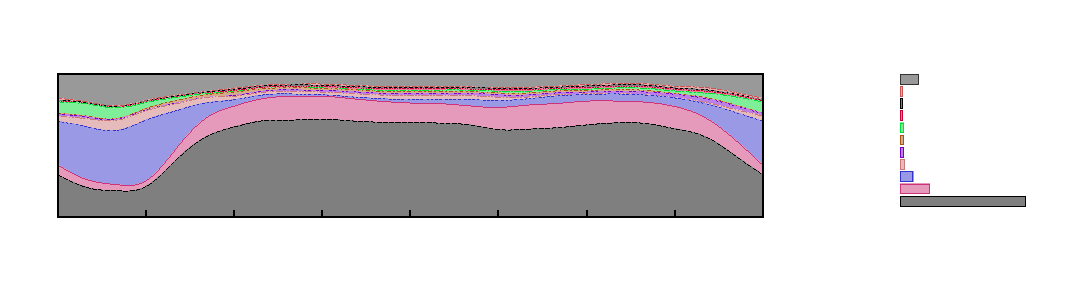
\includegraphics{img/hr-nl}}%
    \gplfronttext
  \end{picture}%
\endgroup


\noindent% GNUPLOT: LaTeX picture with Postscript
\begingroup
  \makeatletter
  \providecommand\color[2][]{%
    \GenericError{(gnuplot) \space\space\space\@spaces}{%
      Package color not loaded in conjunction with
      terminal option `colourtext'%
    }{See the gnuplot documentation for explanation.%
    }{Either use 'blacktext' in gnuplot or load the package
      color.sty in LaTeX.}%
    \renewcommand\color[2][]{}%
  }%
  \providecommand\includegraphics[2][]{%
    \GenericError{(gnuplot) \space\space\space\@spaces}{%
      Package graphicx or graphics not loaded%
    }{See the gnuplot documentation for explanation.%
    }{The gnuplot epslatex terminal needs graphicx.sty or graphics.sty.}%
    \renewcommand\includegraphics[2][]{}%
  }%
  \providecommand\rotatebox[2]{#2}%
  \@ifundefined{ifGPcolor}{%
    \newif\ifGPcolor
    \GPcolorfalse
  }{}%
  \@ifundefined{ifGPblacktext}{%
    \newif\ifGPblacktext
    \GPblacktexttrue
  }{}%
  % define a \g@addto@macro without @ in the name:
  \let\gplgaddtomacro\g@addto@macro
  % define empty templates for all commands taking text:
  \gdef\gplbacktext{}%
  \gdef\gplfronttext{}%
  \makeatother
  \ifGPblacktext
    % no textcolor at all
    \def\colorrgb#1{}%
    \def\colorgray#1{}%
  \else
    % gray or color?
    \ifGPcolor
      \def\colorrgb#1{\color[rgb]{#1}}%
      \def\colorgray#1{\color[gray]{#1}}%
      \expandafter\def\csname LTw\endcsname{\color{white}}%
      \expandafter\def\csname LTb\endcsname{\color{black}}%
      \expandafter\def\csname LTa\endcsname{\color{black}}%
      \expandafter\def\csname LT0\endcsname{\color[rgb]{1,0,0}}%
      \expandafter\def\csname LT1\endcsname{\color[rgb]{0,1,0}}%
      \expandafter\def\csname LT2\endcsname{\color[rgb]{0,0,1}}%
      \expandafter\def\csname LT3\endcsname{\color[rgb]{1,0,1}}%
      \expandafter\def\csname LT4\endcsname{\color[rgb]{0,1,1}}%
      \expandafter\def\csname LT5\endcsname{\color[rgb]{1,1,0}}%
      \expandafter\def\csname LT6\endcsname{\color[rgb]{0,0,0}}%
      \expandafter\def\csname LT7\endcsname{\color[rgb]{1,0.3,0}}%
      \expandafter\def\csname LT8\endcsname{\color[rgb]{0.5,0.5,0.5}}%
    \else
      % gray
      \def\colorrgb#1{\color{black}}%
      \def\colorgray#1{\color[gray]{#1}}%
      \expandafter\def\csname LTw\endcsname{\color{white}}%
      \expandafter\def\csname LTb\endcsname{\color{black}}%
      \expandafter\def\csname LTa\endcsname{\color{black}}%
      \expandafter\def\csname LT0\endcsname{\color{black}}%
      \expandafter\def\csname LT1\endcsname{\color{black}}%
      \expandafter\def\csname LT2\endcsname{\color{black}}%
      \expandafter\def\csname LT3\endcsname{\color{black}}%
      \expandafter\def\csname LT4\endcsname{\color{black}}%
      \expandafter\def\csname LT5\endcsname{\color{black}}%
      \expandafter\def\csname LT6\endcsname{\color{black}}%
      \expandafter\def\csname LT7\endcsname{\color{black}}%
      \expandafter\def\csname LT8\endcsname{\color{black}}%
    \fi
  \fi
  \setlength{\unitlength}{0.0500bp}%
  \begin{picture}(10080.00,2520.00)%
    \gplgaddtomacro\gplbacktext{%
      \csname LTb\endcsname%
      \put(176,1281){\rotatebox{-270}{\makebox(0,0){\strut{}\scriptsize fraction of tweets}}}%
      \put(3779,154){\makebox(0,0){\strut{}\scriptsize time of day (UTC)}}%
      \put(3779,2189){\makebox(0,0){\strut{}Countries that Tweet in Czech}}%
    }%
    \gplgaddtomacro\gplfronttext{%
      \csname LTb\endcsname%
      \put(396,374){\makebox(0,0){\strut{}\scriptsize 0:00}}%
      \put(1242,374){\makebox(0,0){\strut{}\scriptsize 3:00}}%
      \put(2088,374){\makebox(0,0){\strut{}\scriptsize 6:00}}%
      \put(2934,374){\makebox(0,0){\strut{}\scriptsize 9:00}}%
      \put(3780,374){\makebox(0,0){\strut{}\scriptsize 12:00}}%
      \put(4625,374){\makebox(0,0){\strut{}\scriptsize 15:00}}%
      \put(5471,374){\makebox(0,0){\strut{}\scriptsize 18:00}}%
      \put(6317,374){\makebox(0,0){\strut{}\scriptsize 21:00}}%
      \put(7163,374){\makebox(0,0){\strut{}\scriptsize 24:00}}%
    }%
    \gplgaddtomacro\gplbacktext{%
      \csname LTb\endcsname%
      \put(9083,154){\makebox(0,0){\strut{}~~}}%
      \put(9083,2189){\makebox(0,0){\strut{} }}%
    }%
    \gplgaddtomacro\gplfronttext{%
      \csname LTb\endcsname%
      \put(8352,751){\makebox(0,0)[r]{\strut{}\scriptsize~CZ}}%
      \put(8352,868){\makebox(0,0)[r]{\strut{}\scriptsize~Brazil}}%
      \put(8352,985){\makebox(0,0)[r]{\strut{}\scriptsize~USA}}%
      \put(8352,1102){\makebox(0,0)[r]{\strut{}\scriptsize~Spain}}%
      \put(8352,1219){\makebox(0,0)[r]{\strut{}\scriptsize~Philippines}}%
      \put(8352,1337){\makebox(0,0)[r]{\strut{}\scriptsize~Russia}}%
      \put(8352,1454){\makebox(0,0)[r]{\strut{}\scriptsize~UK}}%
      \put(8352,1571){\makebox(0,0)[r]{\strut{}\scriptsize~France}}%
      \put(8352,1688){\makebox(0,0)[r]{\strut{}\scriptsize~South~Africa}}%
      \put(8352,1805){\makebox(0,0)[r]{\strut{}\scriptsize~Italy}}%
      \put(8352,1922){\makebox(0,0)[r]{\strut{}\scriptsize~other}}%
    }%
    \gplbacktext
    \put(0,0){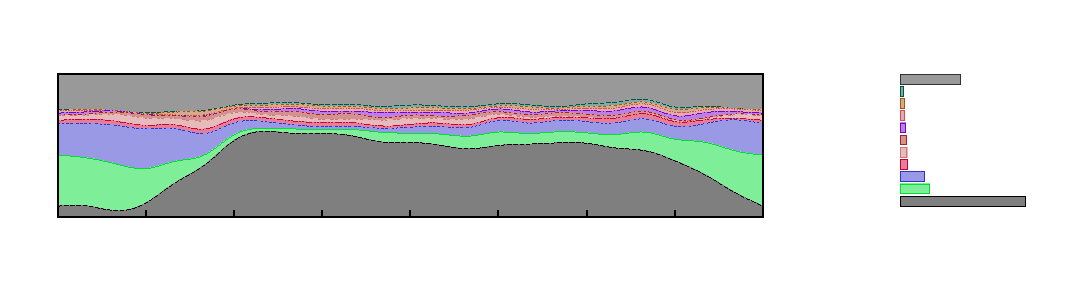
\includegraphics{img/hr-cs}}%
    \gplfronttext
  \end{picture}%
\endgroup


\noindent% GNUPLOT: LaTeX picture with Postscript
\begingroup
  \makeatletter
  \providecommand\color[2][]{%
    \GenericError{(gnuplot) \space\space\space\@spaces}{%
      Package color not loaded in conjunction with
      terminal option `colourtext'%
    }{See the gnuplot documentation for explanation.%
    }{Either use 'blacktext' in gnuplot or load the package
      color.sty in LaTeX.}%
    \renewcommand\color[2][]{}%
  }%
  \providecommand\includegraphics[2][]{%
    \GenericError{(gnuplot) \space\space\space\@spaces}{%
      Package graphicx or graphics not loaded%
    }{See the gnuplot documentation for explanation.%
    }{The gnuplot epslatex terminal needs graphicx.sty or graphics.sty.}%
    \renewcommand\includegraphics[2][]{}%
  }%
  \providecommand\rotatebox[2]{#2}%
  \@ifundefined{ifGPcolor}{%
    \newif\ifGPcolor
    \GPcolorfalse
  }{}%
  \@ifundefined{ifGPblacktext}{%
    \newif\ifGPblacktext
    \GPblacktexttrue
  }{}%
  % define a \g@addto@macro without @ in the name:
  \let\gplgaddtomacro\g@addto@macro
  % define empty templates for all commands taking text:
  \gdef\gplbacktext{}%
  \gdef\gplfronttext{}%
  \makeatother
  \ifGPblacktext
    % no textcolor at all
    \def\colorrgb#1{}%
    \def\colorgray#1{}%
  \else
    % gray or color?
    \ifGPcolor
      \def\colorrgb#1{\color[rgb]{#1}}%
      \def\colorgray#1{\color[gray]{#1}}%
      \expandafter\def\csname LTw\endcsname{\color{white}}%
      \expandafter\def\csname LTb\endcsname{\color{black}}%
      \expandafter\def\csname LTa\endcsname{\color{black}}%
      \expandafter\def\csname LT0\endcsname{\color[rgb]{1,0,0}}%
      \expandafter\def\csname LT1\endcsname{\color[rgb]{0,1,0}}%
      \expandafter\def\csname LT2\endcsname{\color[rgb]{0,0,1}}%
      \expandafter\def\csname LT3\endcsname{\color[rgb]{1,0,1}}%
      \expandafter\def\csname LT4\endcsname{\color[rgb]{0,1,1}}%
      \expandafter\def\csname LT5\endcsname{\color[rgb]{1,1,0}}%
      \expandafter\def\csname LT6\endcsname{\color[rgb]{0,0,0}}%
      \expandafter\def\csname LT7\endcsname{\color[rgb]{1,0.3,0}}%
      \expandafter\def\csname LT8\endcsname{\color[rgb]{0.5,0.5,0.5}}%
    \else
      % gray
      \def\colorrgb#1{\color{black}}%
      \def\colorgray#1{\color[gray]{#1}}%
      \expandafter\def\csname LTw\endcsname{\color{white}}%
      \expandafter\def\csname LTb\endcsname{\color{black}}%
      \expandafter\def\csname LTa\endcsname{\color{black}}%
      \expandafter\def\csname LT0\endcsname{\color{black}}%
      \expandafter\def\csname LT1\endcsname{\color{black}}%
      \expandafter\def\csname LT2\endcsname{\color{black}}%
      \expandafter\def\csname LT3\endcsname{\color{black}}%
      \expandafter\def\csname LT4\endcsname{\color{black}}%
      \expandafter\def\csname LT5\endcsname{\color{black}}%
      \expandafter\def\csname LT6\endcsname{\color{black}}%
      \expandafter\def\csname LT7\endcsname{\color{black}}%
      \expandafter\def\csname LT8\endcsname{\color{black}}%
    \fi
  \fi
  \setlength{\unitlength}{0.0500bp}%
  \begin{picture}(10080.00,2520.00)%
    \gplgaddtomacro\gplbacktext{%
      \csname LTb\endcsname%
      \put(176,1281){\rotatebox{-270}{\makebox(0,0){\strut{}\scriptsize fraction of tweets}}}%
      \put(3779,154){\makebox(0,0){\strut{}\scriptsize time of day (UTC)}}%
      \put(3779,2189){\makebox(0,0){\strut{}Countries that Tweet in Danish}}%
    }%
    \gplgaddtomacro\gplfronttext{%
      \csname LTb\endcsname%
      \put(396,374){\makebox(0,0){\strut{}\scriptsize 0:00}}%
      \put(1242,374){\makebox(0,0){\strut{}\scriptsize 3:00}}%
      \put(2088,374){\makebox(0,0){\strut{}\scriptsize 6:00}}%
      \put(2934,374){\makebox(0,0){\strut{}\scriptsize 9:00}}%
      \put(3780,374){\makebox(0,0){\strut{}\scriptsize 12:00}}%
      \put(4625,374){\makebox(0,0){\strut{}\scriptsize 15:00}}%
      \put(5471,374){\makebox(0,0){\strut{}\scriptsize 18:00}}%
      \put(6317,374){\makebox(0,0){\strut{}\scriptsize 21:00}}%
      \put(7163,374){\makebox(0,0){\strut{}\scriptsize 24:00}}%
    }%
    \gplgaddtomacro\gplbacktext{%
      \csname LTb\endcsname%
      \put(9083,154){\makebox(0,0){\strut{}~~}}%
      \put(9083,2189){\makebox(0,0){\strut{} }}%
    }%
    \gplgaddtomacro\gplfronttext{%
      \csname LTb\endcsname%
      \put(8352,751){\makebox(0,0)[r]{\strut{}\scriptsize~DK}}%
      \put(8352,868){\makebox(0,0)[r]{\strut{}\scriptsize~USA}}%
      \put(8352,985){\makebox(0,0)[r]{\strut{}\scriptsize~Brazil}}%
      \put(8352,1102){\makebox(0,0)[r]{\strut{}\scriptsize~NO}}%
      \put(8352,1219){\makebox(0,0)[r]{\strut{}\scriptsize~Philippines}}%
      \put(8352,1337){\makebox(0,0)[r]{\strut{}\scriptsize~UK}}%
      \put(8352,1454){\makebox(0,0)[r]{\strut{}\scriptsize~Indonesia}}%
      \put(8352,1571){\makebox(0,0)[r]{\strut{}\scriptsize~Malasia}}%
      \put(8352,1688){\makebox(0,0)[r]{\strut{}\scriptsize~SE}}%
      \put(8352,1805){\makebox(0,0)[r]{\strut{}\scriptsize~TR}}%
      \put(8352,1922){\makebox(0,0)[r]{\strut{}\scriptsize~other}}%
    }%
    \gplbacktext
    \put(0,0){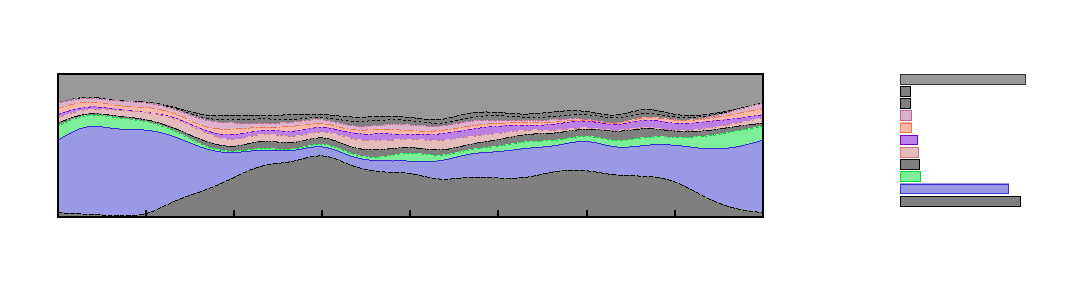
\includegraphics{img/hr-da}}%
    \gplfronttext
  \end{picture}%
\endgroup


\noindent% GNUPLOT: LaTeX picture with Postscript
\begingroup
  \makeatletter
  \providecommand\color[2][]{%
    \GenericError{(gnuplot) \space\space\space\@spaces}{%
      Package color not loaded in conjunction with
      terminal option `colourtext'%
    }{See the gnuplot documentation for explanation.%
    }{Either use 'blacktext' in gnuplot or load the package
      color.sty in LaTeX.}%
    \renewcommand\color[2][]{}%
  }%
  \providecommand\includegraphics[2][]{%
    \GenericError{(gnuplot) \space\space\space\@spaces}{%
      Package graphicx or graphics not loaded%
    }{See the gnuplot documentation for explanation.%
    }{The gnuplot epslatex terminal needs graphicx.sty or graphics.sty.}%
    \renewcommand\includegraphics[2][]{}%
  }%
  \providecommand\rotatebox[2]{#2}%
  \@ifundefined{ifGPcolor}{%
    \newif\ifGPcolor
    \GPcolorfalse
  }{}%
  \@ifundefined{ifGPblacktext}{%
    \newif\ifGPblacktext
    \GPblacktexttrue
  }{}%
  % define a \g@addto@macro without @ in the name:
  \let\gplgaddtomacro\g@addto@macro
  % define empty templates for all commands taking text:
  \gdef\gplbacktext{}%
  \gdef\gplfronttext{}%
  \makeatother
  \ifGPblacktext
    % no textcolor at all
    \def\colorrgb#1{}%
    \def\colorgray#1{}%
  \else
    % gray or color?
    \ifGPcolor
      \def\colorrgb#1{\color[rgb]{#1}}%
      \def\colorgray#1{\color[gray]{#1}}%
      \expandafter\def\csname LTw\endcsname{\color{white}}%
      \expandafter\def\csname LTb\endcsname{\color{black}}%
      \expandafter\def\csname LTa\endcsname{\color{black}}%
      \expandafter\def\csname LT0\endcsname{\color[rgb]{1,0,0}}%
      \expandafter\def\csname LT1\endcsname{\color[rgb]{0,1,0}}%
      \expandafter\def\csname LT2\endcsname{\color[rgb]{0,0,1}}%
      \expandafter\def\csname LT3\endcsname{\color[rgb]{1,0,1}}%
      \expandafter\def\csname LT4\endcsname{\color[rgb]{0,1,1}}%
      \expandafter\def\csname LT5\endcsname{\color[rgb]{1,1,0}}%
      \expandafter\def\csname LT6\endcsname{\color[rgb]{0,0,0}}%
      \expandafter\def\csname LT7\endcsname{\color[rgb]{1,0.3,0}}%
      \expandafter\def\csname LT8\endcsname{\color[rgb]{0.5,0.5,0.5}}%
    \else
      % gray
      \def\colorrgb#1{\color{black}}%
      \def\colorgray#1{\color[gray]{#1}}%
      \expandafter\def\csname LTw\endcsname{\color{white}}%
      \expandafter\def\csname LTb\endcsname{\color{black}}%
      \expandafter\def\csname LTa\endcsname{\color{black}}%
      \expandafter\def\csname LT0\endcsname{\color{black}}%
      \expandafter\def\csname LT1\endcsname{\color{black}}%
      \expandafter\def\csname LT2\endcsname{\color{black}}%
      \expandafter\def\csname LT3\endcsname{\color{black}}%
      \expandafter\def\csname LT4\endcsname{\color{black}}%
      \expandafter\def\csname LT5\endcsname{\color{black}}%
      \expandafter\def\csname LT6\endcsname{\color{black}}%
      \expandafter\def\csname LT7\endcsname{\color{black}}%
      \expandafter\def\csname LT8\endcsname{\color{black}}%
    \fi
  \fi
  \setlength{\unitlength}{0.0500bp}%
  \begin{picture}(10080.00,2520.00)%
    \gplgaddtomacro\gplbacktext{%
      \csname LTb\endcsname%
      \put(176,1281){\rotatebox{-270}{\makebox(0,0){\strut{}\scriptsize fraction of tweets}}}%
      \put(3779,154){\makebox(0,0){\strut{}\scriptsize time of day (UTC)}}%
      \put(3779,2189){\makebox(0,0){\strut{}Countries that Tweet in Greek}}%
    }%
    \gplgaddtomacro\gplfronttext{%
      \csname LTb\endcsname%
      \put(396,374){\makebox(0,0){\strut{}\scriptsize 0:00}}%
      \put(1242,374){\makebox(0,0){\strut{}\scriptsize 3:00}}%
      \put(2088,374){\makebox(0,0){\strut{}\scriptsize 6:00}}%
      \put(2934,374){\makebox(0,0){\strut{}\scriptsize 9:00}}%
      \put(3780,374){\makebox(0,0){\strut{}\scriptsize 12:00}}%
      \put(4625,374){\makebox(0,0){\strut{}\scriptsize 15:00}}%
      \put(5471,374){\makebox(0,0){\strut{}\scriptsize 18:00}}%
      \put(6317,374){\makebox(0,0){\strut{}\scriptsize 21:00}}%
      \put(7163,374){\makebox(0,0){\strut{}\scriptsize 24:00}}%
    }%
    \gplgaddtomacro\gplbacktext{%
      \csname LTb\endcsname%
      \put(9083,154){\makebox(0,0){\strut{}~~}}%
      \put(9083,2189){\makebox(0,0){\strut{} }}%
    }%
    \gplgaddtomacro\gplfronttext{%
      \csname LTb\endcsname%
      \put(8352,751){\makebox(0,0)[r]{\strut{}\scriptsize~GR}}%
      \put(8352,868){\makebox(0,0)[r]{\strut{}\scriptsize~CY}}%
      \put(8352,985){\makebox(0,0)[r]{\strut{}\scriptsize~France}}%
      \put(8352,1102){\makebox(0,0)[r]{\strut{}\scriptsize~UK}}%
      \put(8352,1219){\makebox(0,0)[r]{\strut{}\scriptsize~DE}}%
      \put(8352,1337){\makebox(0,0)[r]{\strut{}\scriptsize~USA}}%
      \put(8352,1454){\makebox(0,0)[r]{\strut{}\scriptsize~CZ}}%
      \put(8352,1571){\makebox(0,0)[r]{\strut{}\scriptsize~Italy}}%
      \put(8352,1688){\makebox(0,0)[r]{\strut{}\scriptsize~Belgium}}%
      \put(8352,1805){\makebox(0,0)[r]{\strut{}\scriptsize~Japan}}%
      \put(8352,1922){\makebox(0,0)[r]{\strut{}\scriptsize~other}}%
    }%
    \gplbacktext
    \put(0,0){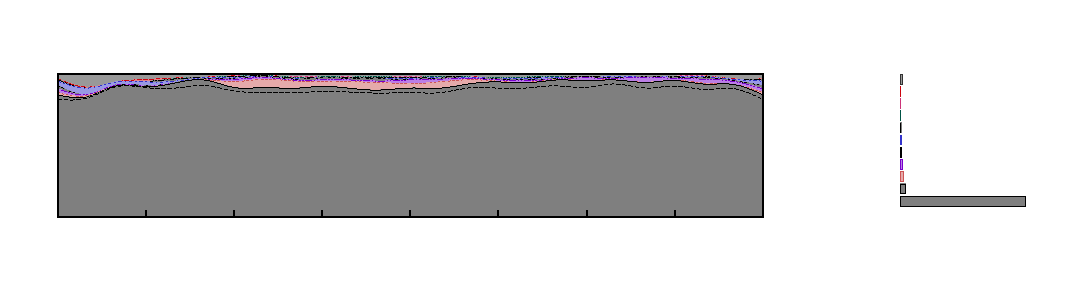
\includegraphics{img/hr-el}}%
    \gplfronttext
  \end{picture}%
\endgroup


\noindent% GNUPLOT: LaTeX picture with Postscript
\begingroup
  \makeatletter
  \providecommand\color[2][]{%
    \GenericError{(gnuplot) \space\space\space\@spaces}{%
      Package color not loaded in conjunction with
      terminal option `colourtext'%
    }{See the gnuplot documentation for explanation.%
    }{Either use 'blacktext' in gnuplot or load the package
      color.sty in LaTeX.}%
    \renewcommand\color[2][]{}%
  }%
  \providecommand\includegraphics[2][]{%
    \GenericError{(gnuplot) \space\space\space\@spaces}{%
      Package graphicx or graphics not loaded%
    }{See the gnuplot documentation for explanation.%
    }{The gnuplot epslatex terminal needs graphicx.sty or graphics.sty.}%
    \renewcommand\includegraphics[2][]{}%
  }%
  \providecommand\rotatebox[2]{#2}%
  \@ifundefined{ifGPcolor}{%
    \newif\ifGPcolor
    \GPcolorfalse
  }{}%
  \@ifundefined{ifGPblacktext}{%
    \newif\ifGPblacktext
    \GPblacktexttrue
  }{}%
  % define a \g@addto@macro without @ in the name:
  \let\gplgaddtomacro\g@addto@macro
  % define empty templates for all commands taking text:
  \gdef\gplbacktext{}%
  \gdef\gplfronttext{}%
  \makeatother
  \ifGPblacktext
    % no textcolor at all
    \def\colorrgb#1{}%
    \def\colorgray#1{}%
  \else
    % gray or color?
    \ifGPcolor
      \def\colorrgb#1{\color[rgb]{#1}}%
      \def\colorgray#1{\color[gray]{#1}}%
      \expandafter\def\csname LTw\endcsname{\color{white}}%
      \expandafter\def\csname LTb\endcsname{\color{black}}%
      \expandafter\def\csname LTa\endcsname{\color{black}}%
      \expandafter\def\csname LT0\endcsname{\color[rgb]{1,0,0}}%
      \expandafter\def\csname LT1\endcsname{\color[rgb]{0,1,0}}%
      \expandafter\def\csname LT2\endcsname{\color[rgb]{0,0,1}}%
      \expandafter\def\csname LT3\endcsname{\color[rgb]{1,0,1}}%
      \expandafter\def\csname LT4\endcsname{\color[rgb]{0,1,1}}%
      \expandafter\def\csname LT5\endcsname{\color[rgb]{1,1,0}}%
      \expandafter\def\csname LT6\endcsname{\color[rgb]{0,0,0}}%
      \expandafter\def\csname LT7\endcsname{\color[rgb]{1,0.3,0}}%
      \expandafter\def\csname LT8\endcsname{\color[rgb]{0.5,0.5,0.5}}%
    \else
      % gray
      \def\colorrgb#1{\color{black}}%
      \def\colorgray#1{\color[gray]{#1}}%
      \expandafter\def\csname LTw\endcsname{\color{white}}%
      \expandafter\def\csname LTb\endcsname{\color{black}}%
      \expandafter\def\csname LTa\endcsname{\color{black}}%
      \expandafter\def\csname LT0\endcsname{\color{black}}%
      \expandafter\def\csname LT1\endcsname{\color{black}}%
      \expandafter\def\csname LT2\endcsname{\color{black}}%
      \expandafter\def\csname LT3\endcsname{\color{black}}%
      \expandafter\def\csname LT4\endcsname{\color{black}}%
      \expandafter\def\csname LT5\endcsname{\color{black}}%
      \expandafter\def\csname LT6\endcsname{\color{black}}%
      \expandafter\def\csname LT7\endcsname{\color{black}}%
      \expandafter\def\csname LT8\endcsname{\color{black}}%
    \fi
  \fi
  \setlength{\unitlength}{0.0500bp}%
  \begin{picture}(10080.00,2520.00)%
    \gplgaddtomacro\gplbacktext{%
      \csname LTb\endcsname%
      \put(176,1281){\rotatebox{-270}{\makebox(0,0){\strut{}\scriptsize fraction of tweets}}}%
      \put(3779,154){\makebox(0,0){\strut{}\scriptsize time of day (UTC)}}%
      \put(3779,2189){\makebox(0,0){\strut{}Countries that Tweet in Polish}}%
    }%
    \gplgaddtomacro\gplfronttext{%
      \csname LTb\endcsname%
      \put(396,374){\makebox(0,0){\strut{}\scriptsize 0:00}}%
      \put(1242,374){\makebox(0,0){\strut{}\scriptsize 3:00}}%
      \put(2088,374){\makebox(0,0){\strut{}\scriptsize 6:00}}%
      \put(2934,374){\makebox(0,0){\strut{}\scriptsize 9:00}}%
      \put(3780,374){\makebox(0,0){\strut{}\scriptsize 12:00}}%
      \put(4625,374){\makebox(0,0){\strut{}\scriptsize 15:00}}%
      \put(5471,374){\makebox(0,0){\strut{}\scriptsize 18:00}}%
      \put(6317,374){\makebox(0,0){\strut{}\scriptsize 21:00}}%
      \put(7163,374){\makebox(0,0){\strut{}\scriptsize 24:00}}%
    }%
    \gplgaddtomacro\gplbacktext{%
      \csname LTb\endcsname%
      \put(9083,154){\makebox(0,0){\strut{}~~}}%
      \put(9083,2189){\makebox(0,0){\strut{} }}%
    }%
    \gplgaddtomacro\gplfronttext{%
      \csname LTb\endcsname%
      \put(8352,751){\makebox(0,0)[r]{\strut{}\scriptsize~PL}}%
      \put(8352,868){\makebox(0,0)[r]{\strut{}\scriptsize~USA}}%
      \put(8352,985){\makebox(0,0)[r]{\strut{}\scriptsize~UK}}%
      \put(8352,1102){\makebox(0,0)[r]{\strut{}\scriptsize~Philippines}}%
      \put(8352,1219){\makebox(0,0)[r]{\strut{}\scriptsize~Brazil}}%
      \put(8352,1337){\makebox(0,0)[r]{\strut{}\scriptsize~Japan}}%
      \put(8352,1454){\makebox(0,0)[r]{\strut{}\scriptsize~South~Africa}}%
      \put(8352,1571){\makebox(0,0)[r]{\strut{}\scriptsize~Nigeria}}%
      \put(8352,1688){\makebox(0,0)[r]{\strut{}\scriptsize~DE}}%
      \put(8352,1805){\makebox(0,0)[r]{\strut{}\scriptsize~NO}}%
      \put(8352,1922){\makebox(0,0)[r]{\strut{}\scriptsize~other}}%
    }%
    \gplbacktext
    \put(0,0){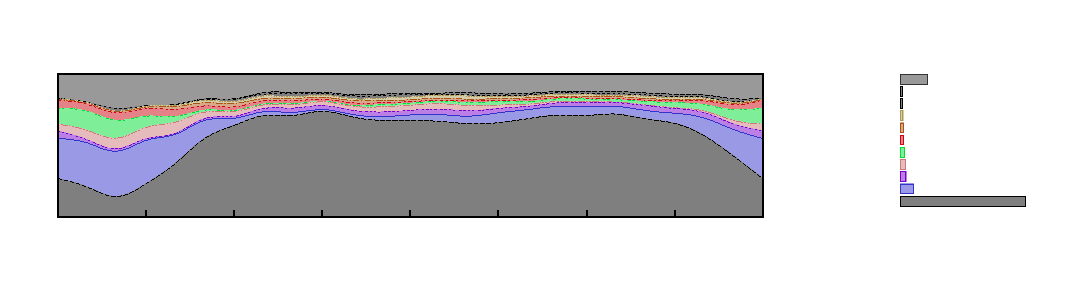
\includegraphics{img/hr-pl}}%
    \gplfronttext
  \end{picture}%
\endgroup


\noindent% GNUPLOT: LaTeX picture with Postscript
\begingroup
  \makeatletter
  \providecommand\color[2][]{%
    \GenericError{(gnuplot) \space\space\space\@spaces}{%
      Package color not loaded in conjunction with
      terminal option `colourtext'%
    }{See the gnuplot documentation for explanation.%
    }{Either use 'blacktext' in gnuplot or load the package
      color.sty in LaTeX.}%
    \renewcommand\color[2][]{}%
  }%
  \providecommand\includegraphics[2][]{%
    \GenericError{(gnuplot) \space\space\space\@spaces}{%
      Package graphicx or graphics not loaded%
    }{See the gnuplot documentation for explanation.%
    }{The gnuplot epslatex terminal needs graphicx.sty or graphics.sty.}%
    \renewcommand\includegraphics[2][]{}%
  }%
  \providecommand\rotatebox[2]{#2}%
  \@ifundefined{ifGPcolor}{%
    \newif\ifGPcolor
    \GPcolorfalse
  }{}%
  \@ifundefined{ifGPblacktext}{%
    \newif\ifGPblacktext
    \GPblacktexttrue
  }{}%
  % define a \g@addto@macro without @ in the name:
  \let\gplgaddtomacro\g@addto@macro
  % define empty templates for all commands taking text:
  \gdef\gplbacktext{}%
  \gdef\gplfronttext{}%
  \makeatother
  \ifGPblacktext
    % no textcolor at all
    \def\colorrgb#1{}%
    \def\colorgray#1{}%
  \else
    % gray or color?
    \ifGPcolor
      \def\colorrgb#1{\color[rgb]{#1}}%
      \def\colorgray#1{\color[gray]{#1}}%
      \expandafter\def\csname LTw\endcsname{\color{white}}%
      \expandafter\def\csname LTb\endcsname{\color{black}}%
      \expandafter\def\csname LTa\endcsname{\color{black}}%
      \expandafter\def\csname LT0\endcsname{\color[rgb]{1,0,0}}%
      \expandafter\def\csname LT1\endcsname{\color[rgb]{0,1,0}}%
      \expandafter\def\csname LT2\endcsname{\color[rgb]{0,0,1}}%
      \expandafter\def\csname LT3\endcsname{\color[rgb]{1,0,1}}%
      \expandafter\def\csname LT4\endcsname{\color[rgb]{0,1,1}}%
      \expandafter\def\csname LT5\endcsname{\color[rgb]{1,1,0}}%
      \expandafter\def\csname LT6\endcsname{\color[rgb]{0,0,0}}%
      \expandafter\def\csname LT7\endcsname{\color[rgb]{1,0.3,0}}%
      \expandafter\def\csname LT8\endcsname{\color[rgb]{0.5,0.5,0.5}}%
    \else
      % gray
      \def\colorrgb#1{\color{black}}%
      \def\colorgray#1{\color[gray]{#1}}%
      \expandafter\def\csname LTw\endcsname{\color{white}}%
      \expandafter\def\csname LTb\endcsname{\color{black}}%
      \expandafter\def\csname LTa\endcsname{\color{black}}%
      \expandafter\def\csname LT0\endcsname{\color{black}}%
      \expandafter\def\csname LT1\endcsname{\color{black}}%
      \expandafter\def\csname LT2\endcsname{\color{black}}%
      \expandafter\def\csname LT3\endcsname{\color{black}}%
      \expandafter\def\csname LT4\endcsname{\color{black}}%
      \expandafter\def\csname LT5\endcsname{\color{black}}%
      \expandafter\def\csname LT6\endcsname{\color{black}}%
      \expandafter\def\csname LT7\endcsname{\color{black}}%
      \expandafter\def\csname LT8\endcsname{\color{black}}%
    \fi
  \fi
  \setlength{\unitlength}{0.0500bp}%
  \begin{picture}(10080.00,2520.00)%
    \gplgaddtomacro\gplbacktext{%
      \csname LTb\endcsname%
      \put(176,1281){\rotatebox{-270}{\makebox(0,0){\strut{}\scriptsize fraction of tweets}}}%
      \put(3779,154){\makebox(0,0){\strut{}\scriptsize time of day (UTC)}}%
      \put(3779,2189){\makebox(0,0){\strut{}Countries that Tweet in Russian}}%
    }%
    \gplgaddtomacro\gplfronttext{%
      \csname LTb\endcsname%
      \put(396,374){\makebox(0,0){\strut{}\scriptsize 0:00}}%
      \put(1242,374){\makebox(0,0){\strut{}\scriptsize 3:00}}%
      \put(2088,374){\makebox(0,0){\strut{}\scriptsize 6:00}}%
      \put(2934,374){\makebox(0,0){\strut{}\scriptsize 9:00}}%
      \put(3780,374){\makebox(0,0){\strut{}\scriptsize 12:00}}%
      \put(4625,374){\makebox(0,0){\strut{}\scriptsize 15:00}}%
      \put(5471,374){\makebox(0,0){\strut{}\scriptsize 18:00}}%
      \put(6317,374){\makebox(0,0){\strut{}\scriptsize 21:00}}%
      \put(7163,374){\makebox(0,0){\strut{}\scriptsize 24:00}}%
    }%
    \gplgaddtomacro\gplbacktext{%
      \csname LTb\endcsname%
      \put(9083,154){\makebox(0,0){\strut{}~~}}%
      \put(9083,2189){\makebox(0,0){\strut{} }}%
    }%
    \gplgaddtomacro\gplfronttext{%
      \csname LTb\endcsname%
      \put(8352,751){\makebox(0,0)[r]{\strut{}\scriptsize~Russia}}%
      \put(8352,868){\makebox(0,0)[r]{\strut{}\scriptsize~UA}}%
      \put(8352,985){\makebox(0,0)[r]{\strut{}\scriptsize~BY}}%
      \put(8352,1102){\makebox(0,0)[r]{\strut{}\scriptsize~MN}}%
      \put(8352,1219){\makebox(0,0)[r]{\strut{}\scriptsize~KZ}}%
      \put(8352,1337){\makebox(0,0)[r]{\strut{}\scriptsize~USA}}%
      \put(8352,1454){\makebox(0,0)[r]{\strut{}\scriptsize~DE}}%
      \put(8352,1571){\makebox(0,0)[r]{\strut{}\scriptsize~PL}}%
      \put(8352,1688){\makebox(0,0)[r]{\strut{}\scriptsize~CZ}}%
      \put(8352,1805){\makebox(0,0)[r]{\strut{}\scriptsize~NL}}%
      \put(8352,1922){\makebox(0,0)[r]{\strut{}\scriptsize~other}}%
    }%
    \gplbacktext
    \put(0,0){\includegraphics{img/hr-ru}}%
    \gplfronttext
  \end{picture}%
\endgroup


\noindent% GNUPLOT: LaTeX picture with Postscript
\begingroup
  \makeatletter
  \providecommand\color[2][]{%
    \GenericError{(gnuplot) \space\space\space\@spaces}{%
      Package color not loaded in conjunction with
      terminal option `colourtext'%
    }{See the gnuplot documentation for explanation.%
    }{Either use 'blacktext' in gnuplot or load the package
      color.sty in LaTeX.}%
    \renewcommand\color[2][]{}%
  }%
  \providecommand\includegraphics[2][]{%
    \GenericError{(gnuplot) \space\space\space\@spaces}{%
      Package graphicx or graphics not loaded%
    }{See the gnuplot documentation for explanation.%
    }{The gnuplot epslatex terminal needs graphicx.sty or graphics.sty.}%
    \renewcommand\includegraphics[2][]{}%
  }%
  \providecommand\rotatebox[2]{#2}%
  \@ifundefined{ifGPcolor}{%
    \newif\ifGPcolor
    \GPcolorfalse
  }{}%
  \@ifundefined{ifGPblacktext}{%
    \newif\ifGPblacktext
    \GPblacktexttrue
  }{}%
  % define a \g@addto@macro without @ in the name:
  \let\gplgaddtomacro\g@addto@macro
  % define empty templates for all commands taking text:
  \gdef\gplbacktext{}%
  \gdef\gplfronttext{}%
  \makeatother
  \ifGPblacktext
    % no textcolor at all
    \def\colorrgb#1{}%
    \def\colorgray#1{}%
  \else
    % gray or color?
    \ifGPcolor
      \def\colorrgb#1{\color[rgb]{#1}}%
      \def\colorgray#1{\color[gray]{#1}}%
      \expandafter\def\csname LTw\endcsname{\color{white}}%
      \expandafter\def\csname LTb\endcsname{\color{black}}%
      \expandafter\def\csname LTa\endcsname{\color{black}}%
      \expandafter\def\csname LT0\endcsname{\color[rgb]{1,0,0}}%
      \expandafter\def\csname LT1\endcsname{\color[rgb]{0,1,0}}%
      \expandafter\def\csname LT2\endcsname{\color[rgb]{0,0,1}}%
      \expandafter\def\csname LT3\endcsname{\color[rgb]{1,0,1}}%
      \expandafter\def\csname LT4\endcsname{\color[rgb]{0,1,1}}%
      \expandafter\def\csname LT5\endcsname{\color[rgb]{1,1,0}}%
      \expandafter\def\csname LT6\endcsname{\color[rgb]{0,0,0}}%
      \expandafter\def\csname LT7\endcsname{\color[rgb]{1,0.3,0}}%
      \expandafter\def\csname LT8\endcsname{\color[rgb]{0.5,0.5,0.5}}%
    \else
      % gray
      \def\colorrgb#1{\color{black}}%
      \def\colorgray#1{\color[gray]{#1}}%
      \expandafter\def\csname LTw\endcsname{\color{white}}%
      \expandafter\def\csname LTb\endcsname{\color{black}}%
      \expandafter\def\csname LTa\endcsname{\color{black}}%
      \expandafter\def\csname LT0\endcsname{\color{black}}%
      \expandafter\def\csname LT1\endcsname{\color{black}}%
      \expandafter\def\csname LT2\endcsname{\color{black}}%
      \expandafter\def\csname LT3\endcsname{\color{black}}%
      \expandafter\def\csname LT4\endcsname{\color{black}}%
      \expandafter\def\csname LT5\endcsname{\color{black}}%
      \expandafter\def\csname LT6\endcsname{\color{black}}%
      \expandafter\def\csname LT7\endcsname{\color{black}}%
      \expandafter\def\csname LT8\endcsname{\color{black}}%
    \fi
  \fi
  \setlength{\unitlength}{0.0500bp}%
  \begin{picture}(10080.00,2520.00)%
    \gplgaddtomacro\gplbacktext{%
      \csname LTb\endcsname%
      \put(176,1281){\rotatebox{-270}{\makebox(0,0){\strut{}\scriptsize fraction of tweets}}}%
      \put(3779,154){\makebox(0,0){\strut{}\scriptsize time of day (UTC)}}%
      \put(3779,2189){\makebox(0,0){\strut{}Countries that Tweet in Vietnamese}}%
    }%
    \gplgaddtomacro\gplfronttext{%
      \csname LTb\endcsname%
      \put(396,374){\makebox(0,0){\strut{}\scriptsize 0:00}}%
      \put(1242,374){\makebox(0,0){\strut{}\scriptsize 3:00}}%
      \put(2088,374){\makebox(0,0){\strut{}\scriptsize 6:00}}%
      \put(2934,374){\makebox(0,0){\strut{}\scriptsize 9:00}}%
      \put(3780,374){\makebox(0,0){\strut{}\scriptsize 12:00}}%
      \put(4625,374){\makebox(0,0){\strut{}\scriptsize 15:00}}%
      \put(5471,374){\makebox(0,0){\strut{}\scriptsize 18:00}}%
      \put(6317,374){\makebox(0,0){\strut{}\scriptsize 21:00}}%
      \put(7163,374){\makebox(0,0){\strut{}\scriptsize 24:00}}%
    }%
    \gplgaddtomacro\gplbacktext{%
      \csname LTb\endcsname%
      \put(9083,154){\makebox(0,0){\strut{}~~}}%
      \put(9083,2189){\makebox(0,0){\strut{} }}%
    }%
    \gplgaddtomacro\gplfronttext{%
      \csname LTb\endcsname%
      \put(8352,751){\makebox(0,0)[r]{\strut{}\scriptsize~VN}}%
      \put(8352,868){\makebox(0,0)[r]{\strut{}\scriptsize~Thailand}}%
      \put(8352,985){\makebox(0,0)[r]{\strut{}\scriptsize~Brazil}}%
      \put(8352,1102){\makebox(0,0)[r]{\strut{}\scriptsize~SN}}%
      \put(8352,1219){\makebox(0,0)[r]{\strut{}\scriptsize~South~Korea}}%
      \put(8352,1337){\makebox(0,0)[r]{\strut{}\scriptsize~USA}}%
      \put(8352,1454){\makebox(0,0)[r]{\strut{}\scriptsize~Philippines}}%
      \put(8352,1571){\makebox(0,0)[r]{\strut{}\scriptsize~Japan}}%
      \put(8352,1688){\makebox(0,0)[r]{\strut{}\scriptsize~India}}%
      \put(8352,1805){\makebox(0,0)[r]{\strut{}\scriptsize~France}}%
      \put(8352,1922){\makebox(0,0)[r]{\strut{}\scriptsize~other}}%
      \put(8484,484){\makebox(0,0){\strut{}\scriptsize 0:00}}%
      \put(8484,484){\makebox(0,0){\strut{}\scriptsize 1:00}}%
      \put(8484,484){\makebox(0,0){\strut{}\scriptsize 2:00}}%
      \put(8484,484){\makebox(0,0){\strut{}\scriptsize 3:00}}%
      \put(8485,484){\makebox(0,0){\strut{}\scriptsize 4:00}}%
      \put(8485,484){\makebox(0,0){\strut{}\scriptsize 5:00}}%
      \put(8485,484){\makebox(0,0){\strut{}\scriptsize 6:00}}%
      \put(8485,484){\makebox(0,0){\strut{}\scriptsize 7:00}}%
      \put(8485,484){\makebox(0,0){\strut{}\scriptsize 8:00}}%
      \put(8485,484){\makebox(0,0){\strut{}\scriptsize 9:00}}%
      \put(8485,484){\makebox(0,0){\strut{}\scriptsize 10:00}}%
      \put(8486,484){\makebox(0,0){\strut{}\scriptsize 11:00}}%
      \put(8486,484){\makebox(0,0){\strut{}\scriptsize 12:00}}%
      \put(8486,484){\makebox(0,0){\strut{}\scriptsize 13:00}}%
      \put(8486,484){\makebox(0,0){\strut{}\scriptsize 14:00}}%
      \put(8486,484){\makebox(0,0){\strut{}\scriptsize 15:00}}%
      \put(8486,484){\makebox(0,0){\strut{}\scriptsize 16:00}}%
      \put(8486,484){\makebox(0,0){\strut{}\scriptsize 17:00}}%
      \put(8487,484){\makebox(0,0){\strut{}\scriptsize 18:00}}%
      \put(8487,484){\makebox(0,0){\strut{}\scriptsize 19:00}}%
      \put(8487,484){\makebox(0,0){\strut{}\scriptsize 20:00}}%
      \put(8487,484){\makebox(0,0){\strut{}\scriptsize 21:00}}%
      \put(8487,484){\makebox(0,0){\strut{}\scriptsize 22:00}}%
      \put(8487,484){\makebox(0,0){\strut{}\scriptsize 23:00}}%
      \put(8487,484){\makebox(0,0){\strut{}\scriptsize 24:00}}%
      \put(8488,484){\makebox(0,0){\strut{}\scriptsize 25:00}}%
      \put(8488,484){\makebox(0,0){\strut{}\scriptsize 26:00}}%
      \put(8488,484){\makebox(0,0){\strut{}\scriptsize 27:00}}%
      \put(8488,484){\makebox(0,0){\strut{}\scriptsize 28:00}}%
      \put(8488,484){\makebox(0,0){\strut{}\scriptsize 29:00}}%
      \put(8488,484){\makebox(0,0){\strut{}\scriptsize 30:00}}%
      \put(8488,484){\makebox(0,0){\strut{}\scriptsize 31:00}}%
      \put(8489,484){\makebox(0,0){\strut{}\scriptsize 32:00}}%
      \put(8489,484){\makebox(0,0){\strut{}\scriptsize 33:00}}%
      \put(8489,484){\makebox(0,0){\strut{}\scriptsize 34:00}}%
      \put(8489,484){\makebox(0,0){\strut{}\scriptsize 35:00}}%
      \put(8489,484){\makebox(0,0){\strut{}\scriptsize 36:00}}%
      \put(8489,484){\makebox(0,0){\strut{}\scriptsize 37:00}}%
      \put(8489,484){\makebox(0,0){\strut{}\scriptsize 38:00}}%
      \put(8490,484){\makebox(0,0){\strut{}\scriptsize 39:00}}%
      \put(8490,484){\makebox(0,0){\strut{}\scriptsize 40:00}}%
      \put(8490,484){\makebox(0,0){\strut{}\scriptsize 41:00}}%
      \put(8490,484){\makebox(0,0){\strut{}\scriptsize 42:00}}%
      \put(8490,484){\makebox(0,0){\strut{}\scriptsize 43:00}}%
      \put(8490,484){\makebox(0,0){\strut{}\scriptsize 44:00}}%
      \put(8490,484){\makebox(0,0){\strut{}\scriptsize 45:00}}%
      \put(8491,484){\makebox(0,0){\strut{}\scriptsize 46:00}}%
      \put(8491,484){\makebox(0,0){\strut{}\scriptsize 47:00}}%
      \put(8491,484){\makebox(0,0){\strut{}\scriptsize 48:00}}%
      \put(8491,484){\makebox(0,0){\strut{}\scriptsize 49:00}}%
      \put(8491,484){\makebox(0,0){\strut{}\scriptsize 50:00}}%
      \put(8491,484){\makebox(0,0){\strut{}\scriptsize 51:00}}%
      \put(8491,484){\makebox(0,0){\strut{}\scriptsize 52:00}}%
      \put(8492,484){\makebox(0,0){\strut{}\scriptsize 53:00}}%
      \put(8492,484){\makebox(0,0){\strut{}\scriptsize 54:00}}%
      \put(8492,484){\makebox(0,0){\strut{}\scriptsize 55:00}}%
      \put(8492,484){\makebox(0,0){\strut{}\scriptsize 56:00}}%
      \put(8492,484){\makebox(0,0){\strut{}\scriptsize 57:00}}%
      \put(8492,484){\makebox(0,0){\strut{}\scriptsize 58:00}}%
      \put(8492,484){\makebox(0,0){\strut{}\scriptsize 59:00}}%
      \put(8493,484){\makebox(0,0){\strut{}\scriptsize 60:00}}%
      \put(8493,484){\makebox(0,0){\strut{}\scriptsize 61:00}}%
      \put(8493,484){\makebox(0,0){\strut{}\scriptsize 62:00}}%
      \put(8493,484){\makebox(0,0){\strut{}\scriptsize 63:00}}%
      \put(8493,484){\makebox(0,0){\strut{}\scriptsize 64:00}}%
      \put(8493,484){\makebox(0,0){\strut{}\scriptsize 65:00}}%
      \put(8493,484){\makebox(0,0){\strut{}\scriptsize 66:00}}%
      \put(8494,484){\makebox(0,0){\strut{}\scriptsize 67:00}}%
      \put(8494,484){\makebox(0,0){\strut{}\scriptsize 68:00}}%
      \put(8494,484){\makebox(0,0){\strut{}\scriptsize 69:00}}%
      \put(8494,484){\makebox(0,0){\strut{}\scriptsize 70:00}}%
      \put(8494,484){\makebox(0,0){\strut{}\scriptsize 71:00}}%
      \put(8494,484){\makebox(0,0){\strut{}\scriptsize 72:00}}%
      \put(8494,484){\makebox(0,0){\strut{}\scriptsize 73:00}}%
      \put(8495,484){\makebox(0,0){\strut{}\scriptsize 74:00}}%
      \put(8495,484){\makebox(0,0){\strut{}\scriptsize 75:00}}%
      \put(8495,484){\makebox(0,0){\strut{}\scriptsize 76:00}}%
      \put(8495,484){\makebox(0,0){\strut{}\scriptsize 77:00}}%
      \put(8495,484){\makebox(0,0){\strut{}\scriptsize 78:00}}%
      \put(8495,484){\makebox(0,0){\strut{}\scriptsize 79:00}}%
      \put(8495,484){\makebox(0,0){\strut{}\scriptsize 80:00}}%
      \put(8496,484){\makebox(0,0){\strut{}\scriptsize 81:00}}%
      \put(8496,484){\makebox(0,0){\strut{}\scriptsize 82:00}}%
      \put(8496,484){\makebox(0,0){\strut{}\scriptsize 83:00}}%
      \put(8496,484){\makebox(0,0){\strut{}\scriptsize 84:00}}%
      \put(8496,484){\makebox(0,0){\strut{}\scriptsize 85:00}}%
      \put(8496,484){\makebox(0,0){\strut{}\scriptsize 86:00}}%
      \put(8496,484){\makebox(0,0){\strut{}\scriptsize 87:00}}%
      \put(8497,484){\makebox(0,0){\strut{}\scriptsize 88:00}}%
      \put(8497,484){\makebox(0,0){\strut{}\scriptsize 89:00}}%
      \put(8497,484){\makebox(0,0){\strut{}\scriptsize 90:00}}%
      \put(8497,484){\makebox(0,0){\strut{}\scriptsize 91:00}}%
      \put(8497,484){\makebox(0,0){\strut{}\scriptsize 92:00}}%
      \put(8497,484){\makebox(0,0){\strut{}\scriptsize 93:00}}%
      \put(8497,484){\makebox(0,0){\strut{}\scriptsize 94:00}}%
      \put(8498,484){\makebox(0,0){\strut{}\scriptsize 95:00}}%
      \put(8498,484){\makebox(0,0){\strut{}\scriptsize 96:00}}%
      \put(8498,484){\makebox(0,0){\strut{}\scriptsize 97:00}}%
      \put(8498,484){\makebox(0,0){\strut{}\scriptsize 98:00}}%
      \put(8498,484){\makebox(0,0){\strut{}\scriptsize 99:00}}%
      \put(8498,484){\makebox(0,0){\strut{}\scriptsize 100:00}}%
      \put(8498,484){\makebox(0,0){\strut{}\scriptsize 101:00}}%
      \put(8499,484){\makebox(0,0){\strut{}\scriptsize 102:00}}%
      \put(8499,484){\makebox(0,0){\strut{}\scriptsize 103:00}}%
      \put(8499,484){\makebox(0,0){\strut{}\scriptsize 104:00}}%
      \put(8499,484){\makebox(0,0){\strut{}\scriptsize 105:00}}%
      \put(8499,484){\makebox(0,0){\strut{}\scriptsize 106:00}}%
      \put(8499,484){\makebox(0,0){\strut{}\scriptsize 107:00}}%
      \put(8499,484){\makebox(0,0){\strut{}\scriptsize 108:00}}%
      \put(8500,484){\makebox(0,0){\strut{}\scriptsize 109:00}}%
      \put(8500,484){\makebox(0,0){\strut{}\scriptsize 110:00}}%
      \put(8500,484){\makebox(0,0){\strut{}\scriptsize 111:00}}%
      \put(8500,484){\makebox(0,0){\strut{}\scriptsize 112:00}}%
      \put(8500,484){\makebox(0,0){\strut{}\scriptsize 113:00}}%
      \put(8500,484){\makebox(0,0){\strut{}\scriptsize 114:00}}%
      \put(8500,484){\makebox(0,0){\strut{}\scriptsize 115:00}}%
      \put(8501,484){\makebox(0,0){\strut{}\scriptsize 116:00}}%
      \put(8501,484){\makebox(0,0){\strut{}\scriptsize 117:00}}%
      \put(8501,484){\makebox(0,0){\strut{}\scriptsize 118:00}}%
      \put(8501,484){\makebox(0,0){\strut{}\scriptsize 119:00}}%
      \put(8501,484){\makebox(0,0){\strut{}\scriptsize 120:00}}%
      \put(8501,484){\makebox(0,0){\strut{}\scriptsize 121:00}}%
      \put(8501,484){\makebox(0,0){\strut{}\scriptsize 122:00}}%
      \put(8502,484){\makebox(0,0){\strut{}\scriptsize 123:00}}%
      \put(8502,484){\makebox(0,0){\strut{}\scriptsize 124:00}}%
      \put(8502,484){\makebox(0,0){\strut{}\scriptsize 125:00}}%
      \put(8502,484){\makebox(0,0){\strut{}\scriptsize 126:00}}%
      \put(8502,484){\makebox(0,0){\strut{}\scriptsize 127:00}}%
      \put(8502,484){\makebox(0,0){\strut{}\scriptsize 128:00}}%
      \put(8502,484){\makebox(0,0){\strut{}\scriptsize 129:00}}%
      \put(8503,484){\makebox(0,0){\strut{}\scriptsize 130:00}}%
      \put(8503,484){\makebox(0,0){\strut{}\scriptsize 131:00}}%
      \put(8503,484){\makebox(0,0){\strut{}\scriptsize 132:00}}%
      \put(8503,484){\makebox(0,0){\strut{}\scriptsize 133:00}}%
      \put(8503,484){\makebox(0,0){\strut{}\scriptsize 134:00}}%
      \put(8503,484){\makebox(0,0){\strut{}\scriptsize 135:00}}%
      \put(8503,484){\makebox(0,0){\strut{}\scriptsize 136:00}}%
      \put(8504,484){\makebox(0,0){\strut{}\scriptsize 137:00}}%
      \put(8504,484){\makebox(0,0){\strut{}\scriptsize 138:00}}%
      \put(8504,484){\makebox(0,0){\strut{}\scriptsize 139:00}}%
      \put(8504,484){\makebox(0,0){\strut{}\scriptsize 140:00}}%
      \put(8504,484){\makebox(0,0){\strut{}\scriptsize 141:00}}%
      \put(8504,484){\makebox(0,0){\strut{}\scriptsize 142:00}}%
      \put(8504,484){\makebox(0,0){\strut{}\scriptsize 143:00}}%
      \put(8505,484){\makebox(0,0){\strut{}\scriptsize 144:00}}%
      \put(8505,484){\makebox(0,0){\strut{}\scriptsize 145:00}}%
      \put(8505,484){\makebox(0,0){\strut{}\scriptsize 146:00}}%
      \put(8505,484){\makebox(0,0){\strut{}\scriptsize 147:00}}%
      \put(8505,484){\makebox(0,0){\strut{}\scriptsize 148:00}}%
      \put(8505,484){\makebox(0,0){\strut{}\scriptsize 149:00}}%
      \put(8505,484){\makebox(0,0){\strut{}\scriptsize 150:00}}%
      \put(8506,484){\makebox(0,0){\strut{}\scriptsize 151:00}}%
      \put(8506,484){\makebox(0,0){\strut{}\scriptsize 152:00}}%
      \put(8506,484){\makebox(0,0){\strut{}\scriptsize 153:00}}%
      \put(8506,484){\makebox(0,0){\strut{}\scriptsize 154:00}}%
      \put(8506,484){\makebox(0,0){\strut{}\scriptsize 155:00}}%
      \put(8506,484){\makebox(0,0){\strut{}\scriptsize 156:00}}%
      \put(8506,484){\makebox(0,0){\strut{}\scriptsize 157:00}}%
      \put(8507,484){\makebox(0,0){\strut{}\scriptsize 158:00}}%
      \put(8507,484){\makebox(0,0){\strut{}\scriptsize 159:00}}%
      \put(8507,484){\makebox(0,0){\strut{}\scriptsize 160:00}}%
      \put(8507,484){\makebox(0,0){\strut{}\scriptsize 161:00}}%
      \put(8507,484){\makebox(0,0){\strut{}\scriptsize 162:00}}%
      \put(8507,484){\makebox(0,0){\strut{}\scriptsize 163:00}}%
      \put(8507,484){\makebox(0,0){\strut{}\scriptsize 164:00}}%
      \put(8508,484){\makebox(0,0){\strut{}\scriptsize 165:00}}%
      \put(8508,484){\makebox(0,0){\strut{}\scriptsize 166:00}}%
      \put(8508,484){\makebox(0,0){\strut{}\scriptsize 167:00}}%
      \put(8508,484){\makebox(0,0){\strut{}\scriptsize 168:00}}%
      \put(8508,484){\makebox(0,0){\strut{}\scriptsize 169:00}}%
      \put(8508,484){\makebox(0,0){\strut{}\scriptsize 170:00}}%
      \put(8508,484){\makebox(0,0){\strut{}\scriptsize 171:00}}%
      \put(8509,484){\makebox(0,0){\strut{}\scriptsize 172:00}}%
      \put(8509,484){\makebox(0,0){\strut{}\scriptsize 173:00}}%
      \put(8509,484){\makebox(0,0){\strut{}\scriptsize 174:00}}%
      \put(8509,484){\makebox(0,0){\strut{}\scriptsize 175:00}}%
      \put(8509,484){\makebox(0,0){\strut{}\scriptsize 176:00}}%
      \put(8509,484){\makebox(0,0){\strut{}\scriptsize 177:00}}%
      \put(8509,484){\makebox(0,0){\strut{}\scriptsize 178:00}}%
      \put(8510,484){\makebox(0,0){\strut{}\scriptsize 179:00}}%
      \put(8510,484){\makebox(0,0){\strut{}\scriptsize 180:00}}%
      \put(8510,484){\makebox(0,0){\strut{}\scriptsize 181:00}}%
      \put(8510,484){\makebox(0,0){\strut{}\scriptsize 182:00}}%
      \put(8510,484){\makebox(0,0){\strut{}\scriptsize 183:00}}%
      \put(8510,484){\makebox(0,0){\strut{}\scriptsize 184:00}}%
      \put(8510,484){\makebox(0,0){\strut{}\scriptsize 185:00}}%
      \put(8511,484){\makebox(0,0){\strut{}\scriptsize 186:00}}%
      \put(8511,484){\makebox(0,0){\strut{}\scriptsize 187:00}}%
      \put(8511,484){\makebox(0,0){\strut{}\scriptsize 188:00}}%
      \put(8511,484){\makebox(0,0){\strut{}\scriptsize 189:00}}%
      \put(8511,484){\makebox(0,0){\strut{}\scriptsize 190:00}}%
      \put(8511,484){\makebox(0,0){\strut{}\scriptsize 191:00}}%
      \put(8511,484){\makebox(0,0){\strut{}\scriptsize 192:00}}%
      \put(8512,484){\makebox(0,0){\strut{}\scriptsize 193:00}}%
      \put(8512,484){\makebox(0,0){\strut{}\scriptsize 194:00}}%
      \put(8512,484){\makebox(0,0){\strut{}\scriptsize 195:00}}%
      \put(8512,484){\makebox(0,0){\strut{}\scriptsize 196:00}}%
      \put(8512,484){\makebox(0,0){\strut{}\scriptsize 197:00}}%
      \put(8512,484){\makebox(0,0){\strut{}\scriptsize 198:00}}%
      \put(8512,484){\makebox(0,0){\strut{}\scriptsize 199:00}}%
      \put(8513,484){\makebox(0,0){\strut{}\scriptsize 200:00}}%
      \put(8513,484){\makebox(0,0){\strut{}\scriptsize 201:00}}%
      \put(8513,484){\makebox(0,0){\strut{}\scriptsize 202:00}}%
      \put(8513,484){\makebox(0,0){\strut{}\scriptsize 203:00}}%
      \put(8513,484){\makebox(0,0){\strut{}\scriptsize 204:00}}%
      \put(8513,484){\makebox(0,0){\strut{}\scriptsize 205:00}}%
      \put(8513,484){\makebox(0,0){\strut{}\scriptsize 206:00}}%
      \put(8514,484){\makebox(0,0){\strut{}\scriptsize 207:00}}%
      \put(8514,484){\makebox(0,0){\strut{}\scriptsize 208:00}}%
      \put(8514,484){\makebox(0,0){\strut{}\scriptsize 209:00}}%
      \put(8514,484){\makebox(0,0){\strut{}\scriptsize 210:00}}%
      \put(8514,484){\makebox(0,0){\strut{}\scriptsize 211:00}}%
      \put(8514,484){\makebox(0,0){\strut{}\scriptsize 212:00}}%
      \put(8514,484){\makebox(0,0){\strut{}\scriptsize 213:00}}%
      \put(8515,484){\makebox(0,0){\strut{}\scriptsize 214:00}}%
      \put(8515,484){\makebox(0,0){\strut{}\scriptsize 215:00}}%
      \put(8515,484){\makebox(0,0){\strut{}\scriptsize 216:00}}%
      \put(8515,484){\makebox(0,0){\strut{}\scriptsize 217:00}}%
      \put(8515,484){\makebox(0,0){\strut{}\scriptsize 218:00}}%
      \put(8515,484){\makebox(0,0){\strut{}\scriptsize 219:00}}%
      \put(8515,484){\makebox(0,0){\strut{}\scriptsize 220:00}}%
      \put(8516,484){\makebox(0,0){\strut{}\scriptsize 221:00}}%
      \put(8516,484){\makebox(0,0){\strut{}\scriptsize 222:00}}%
      \put(8516,484){\makebox(0,0){\strut{}\scriptsize 223:00}}%
      \put(8516,484){\makebox(0,0){\strut{}\scriptsize 224:00}}%
      \put(8516,484){\makebox(0,0){\strut{}\scriptsize 225:00}}%
      \put(8516,484){\makebox(0,0){\strut{}\scriptsize 226:00}}%
      \put(8516,484){\makebox(0,0){\strut{}\scriptsize 227:00}}%
      \put(8517,484){\makebox(0,0){\strut{}\scriptsize 228:00}}%
      \put(8517,484){\makebox(0,0){\strut{}\scriptsize 229:00}}%
      \put(8517,484){\makebox(0,0){\strut{}\scriptsize 230:00}}%
      \put(8517,484){\makebox(0,0){\strut{}\scriptsize 231:00}}%
      \put(8517,484){\makebox(0,0){\strut{}\scriptsize 232:00}}%
      \put(8517,484){\makebox(0,0){\strut{}\scriptsize 233:00}}%
      \put(8517,484){\makebox(0,0){\strut{}\scriptsize 234:00}}%
      \put(8518,484){\makebox(0,0){\strut{}\scriptsize 235:00}}%
      \put(8518,484){\makebox(0,0){\strut{}\scriptsize 236:00}}%
      \put(8518,484){\makebox(0,0){\strut{}\scriptsize 237:00}}%
      \put(8518,484){\makebox(0,0){\strut{}\scriptsize 238:00}}%
      \put(8518,484){\makebox(0,0){\strut{}\scriptsize 239:00}}%
      \put(8518,484){\makebox(0,0){\strut{}\scriptsize 240:00}}%
      \put(8518,484){\makebox(0,0){\strut{}\scriptsize 241:00}}%
      \put(8519,484){\makebox(0,0){\strut{}\scriptsize 242:00}}%
      \put(8519,484){\makebox(0,0){\strut{}\scriptsize 243:00}}%
      \put(8519,484){\makebox(0,0){\strut{}\scriptsize 244:00}}%
      \put(8519,484){\makebox(0,0){\strut{}\scriptsize 245:00}}%
      \put(8519,484){\makebox(0,0){\strut{}\scriptsize 246:00}}%
      \put(8519,484){\makebox(0,0){\strut{}\scriptsize 247:00}}%
      \put(8519,484){\makebox(0,0){\strut{}\scriptsize 248:00}}%
      \put(8520,484){\makebox(0,0){\strut{}\scriptsize 249:00}}%
      \put(8520,484){\makebox(0,0){\strut{}\scriptsize 250:00}}%
      \put(8520,484){\makebox(0,0){\strut{}\scriptsize 251:00}}%
      \put(8520,484){\makebox(0,0){\strut{}\scriptsize 252:00}}%
      \put(8520,484){\makebox(0,0){\strut{}\scriptsize 253:00}}%
      \put(8520,484){\makebox(0,0){\strut{}\scriptsize 254:00}}%
      \put(8520,484){\makebox(0,0){\strut{}\scriptsize 255:00}}%
      \put(8521,484){\makebox(0,0){\strut{}\scriptsize 256:00}}%
      \put(8521,484){\makebox(0,0){\strut{}\scriptsize 257:00}}%
      \put(8521,484){\makebox(0,0){\strut{}\scriptsize 258:00}}%
      \put(8521,484){\makebox(0,0){\strut{}\scriptsize 259:00}}%
      \put(8521,484){\makebox(0,0){\strut{}\scriptsize 260:00}}%
      \put(8521,484){\makebox(0,0){\strut{}\scriptsize 261:00}}%
      \put(8521,484){\makebox(0,0){\strut{}\scriptsize 262:00}}%
      \put(8522,484){\makebox(0,0){\strut{}\scriptsize 263:00}}%
      \put(8522,484){\makebox(0,0){\strut{}\scriptsize 264:00}}%
      \put(8522,484){\makebox(0,0){\strut{}\scriptsize 265:00}}%
      \put(8522,484){\makebox(0,0){\strut{}\scriptsize 266:00}}%
      \put(8522,484){\makebox(0,0){\strut{}\scriptsize 267:00}}%
      \put(8522,484){\makebox(0,0){\strut{}\scriptsize 268:00}}%
      \put(8522,484){\makebox(0,0){\strut{}\scriptsize 269:00}}%
      \put(8523,484){\makebox(0,0){\strut{}\scriptsize 270:00}}%
      \put(8523,484){\makebox(0,0){\strut{}\scriptsize 271:00}}%
      \put(8523,484){\makebox(0,0){\strut{}\scriptsize 272:00}}%
      \put(8523,484){\makebox(0,0){\strut{}\scriptsize 273:00}}%
      \put(8523,484){\makebox(0,0){\strut{}\scriptsize 274:00}}%
      \put(8523,484){\makebox(0,0){\strut{}\scriptsize 275:00}}%
      \put(8523,484){\makebox(0,0){\strut{}\scriptsize 276:00}}%
      \put(8524,484){\makebox(0,0){\strut{}\scriptsize 277:00}}%
      \put(8524,484){\makebox(0,0){\strut{}\scriptsize 278:00}}%
      \put(8524,484){\makebox(0,0){\strut{}\scriptsize 279:00}}%
      \put(8524,484){\makebox(0,0){\strut{}\scriptsize 280:00}}%
      \put(8524,484){\makebox(0,0){\strut{}\scriptsize 281:00}}%
      \put(8524,484){\makebox(0,0){\strut{}\scriptsize 282:00}}%
      \put(8524,484){\makebox(0,0){\strut{}\scriptsize 283:00}}%
      \put(8525,484){\makebox(0,0){\strut{}\scriptsize 284:00}}%
      \put(8525,484){\makebox(0,0){\strut{}\scriptsize 285:00}}%
      \put(8525,484){\makebox(0,0){\strut{}\scriptsize 286:00}}%
      \put(8525,484){\makebox(0,0){\strut{}\scriptsize 287:00}}%
      \put(8525,484){\makebox(0,0){\strut{}\scriptsize 288:00}}%
      \put(8525,484){\makebox(0,0){\strut{}\scriptsize 289:00}}%
      \put(8525,484){\makebox(0,0){\strut{}\scriptsize 290:00}}%
      \put(8526,484){\makebox(0,0){\strut{}\scriptsize 291:00}}%
      \put(8526,484){\makebox(0,0){\strut{}\scriptsize 292:00}}%
      \put(8526,484){\makebox(0,0){\strut{}\scriptsize 293:00}}%
      \put(8526,484){\makebox(0,0){\strut{}\scriptsize 294:00}}%
      \put(8526,484){\makebox(0,0){\strut{}\scriptsize 295:00}}%
      \put(8526,484){\makebox(0,0){\strut{}\scriptsize 296:00}}%
      \put(8526,484){\makebox(0,0){\strut{}\scriptsize 297:00}}%
      \put(8527,484){\makebox(0,0){\strut{}\scriptsize 298:00}}%
      \put(8527,484){\makebox(0,0){\strut{}\scriptsize 299:00}}%
      \put(8527,484){\makebox(0,0){\strut{}\scriptsize 300:00}}%
      \put(8527,484){\makebox(0,0){\strut{}\scriptsize 301:00}}%
      \put(8527,484){\makebox(0,0){\strut{}\scriptsize 302:00}}%
      \put(8527,484){\makebox(0,0){\strut{}\scriptsize 303:00}}%
      \put(8527,484){\makebox(0,0){\strut{}\scriptsize 304:00}}%
      \put(8528,484){\makebox(0,0){\strut{}\scriptsize 305:00}}%
      \put(8528,484){\makebox(0,0){\strut{}\scriptsize 306:00}}%
      \put(8528,484){\makebox(0,0){\strut{}\scriptsize 307:00}}%
      \put(8528,484){\makebox(0,0){\strut{}\scriptsize 308:00}}%
      \put(8528,484){\makebox(0,0){\strut{}\scriptsize 309:00}}%
      \put(8528,484){\makebox(0,0){\strut{}\scriptsize 310:00}}%
      \put(8528,484){\makebox(0,0){\strut{}\scriptsize 311:00}}%
      \put(8529,484){\makebox(0,0){\strut{}\scriptsize 312:00}}%
      \put(8529,484){\makebox(0,0){\strut{}\scriptsize 313:00}}%
      \put(8529,484){\makebox(0,0){\strut{}\scriptsize 314:00}}%
      \put(8529,484){\makebox(0,0){\strut{}\scriptsize 315:00}}%
      \put(8529,484){\makebox(0,0){\strut{}\scriptsize 316:00}}%
      \put(8529,484){\makebox(0,0){\strut{}\scriptsize 317:00}}%
      \put(8529,484){\makebox(0,0){\strut{}\scriptsize 318:00}}%
      \put(8530,484){\makebox(0,0){\strut{}\scriptsize 319:00}}%
      \put(8530,484){\makebox(0,0){\strut{}\scriptsize 320:00}}%
      \put(8530,484){\makebox(0,0){\strut{}\scriptsize 321:00}}%
      \put(8530,484){\makebox(0,0){\strut{}\scriptsize 322:00}}%
      \put(8530,484){\makebox(0,0){\strut{}\scriptsize 323:00}}%
      \put(8530,484){\makebox(0,0){\strut{}\scriptsize 324:00}}%
      \put(8530,484){\makebox(0,0){\strut{}\scriptsize 325:00}}%
      \put(8531,484){\makebox(0,0){\strut{}\scriptsize 326:00}}%
      \put(8531,484){\makebox(0,0){\strut{}\scriptsize 327:00}}%
      \put(8531,484){\makebox(0,0){\strut{}\scriptsize 328:00}}%
      \put(8531,484){\makebox(0,0){\strut{}\scriptsize 329:00}}%
      \put(8531,484){\makebox(0,0){\strut{}\scriptsize 330:00}}%
      \put(8531,484){\makebox(0,0){\strut{}\scriptsize 331:00}}%
      \put(8531,484){\makebox(0,0){\strut{}\scriptsize 332:00}}%
      \put(8532,484){\makebox(0,0){\strut{}\scriptsize 333:00}}%
      \put(8532,484){\makebox(0,0){\strut{}\scriptsize 334:00}}%
      \put(8532,484){\makebox(0,0){\strut{}\scriptsize 335:00}}%
      \put(8532,484){\makebox(0,0){\strut{}\scriptsize 336:00}}%
      \put(8532,484){\makebox(0,0){\strut{}\scriptsize 337:00}}%
      \put(8532,484){\makebox(0,0){\strut{}\scriptsize 338:00}}%
      \put(8532,484){\makebox(0,0){\strut{}\scriptsize 339:00}}%
      \put(8533,484){\makebox(0,0){\strut{}\scriptsize 340:00}}%
      \put(8533,484){\makebox(0,0){\strut{}\scriptsize 341:00}}%
      \put(8533,484){\makebox(0,0){\strut{}\scriptsize 342:00}}%
      \put(8533,484){\makebox(0,0){\strut{}\scriptsize 343:00}}%
      \put(8533,484){\makebox(0,0){\strut{}\scriptsize 344:00}}%
      \put(8533,484){\makebox(0,0){\strut{}\scriptsize 345:00}}%
      \put(8533,484){\makebox(0,0){\strut{}\scriptsize 346:00}}%
      \put(8534,484){\makebox(0,0){\strut{}\scriptsize 347:00}}%
      \put(8534,484){\makebox(0,0){\strut{}\scriptsize 348:00}}%
      \put(8534,484){\makebox(0,0){\strut{}\scriptsize 349:00}}%
      \put(8534,484){\makebox(0,0){\strut{}\scriptsize 350:00}}%
      \put(8534,484){\makebox(0,0){\strut{}\scriptsize 351:00}}%
      \put(8534,484){\makebox(0,0){\strut{}\scriptsize 352:00}}%
      \put(8534,484){\makebox(0,0){\strut{}\scriptsize 353:00}}%
      \put(8535,484){\makebox(0,0){\strut{}\scriptsize 354:00}}%
      \put(8535,484){\makebox(0,0){\strut{}\scriptsize 355:00}}%
      \put(8535,484){\makebox(0,0){\strut{}\scriptsize 356:00}}%
      \put(8535,484){\makebox(0,0){\strut{}\scriptsize 357:00}}%
      \put(8535,484){\makebox(0,0){\strut{}\scriptsize 358:00}}%
      \put(8535,484){\makebox(0,0){\strut{}\scriptsize 359:00}}%
      \put(8535,484){\makebox(0,0){\strut{}\scriptsize 360:00}}%
      \put(8536,484){\makebox(0,0){\strut{}\scriptsize 361:00}}%
      \put(8536,484){\makebox(0,0){\strut{}\scriptsize 362:00}}%
      \put(8536,484){\makebox(0,0){\strut{}\scriptsize 363:00}}%
      \put(8536,484){\makebox(0,0){\strut{}\scriptsize 364:00}}%
      \put(8536,484){\makebox(0,0){\strut{}\scriptsize 365:00}}%
      \put(8536,484){\makebox(0,0){\strut{}\scriptsize 366:00}}%
      \put(8536,484){\makebox(0,0){\strut{}\scriptsize 367:00}}%
      \put(8537,484){\makebox(0,0){\strut{}\scriptsize 368:00}}%
      \put(8537,484){\makebox(0,0){\strut{}\scriptsize 369:00}}%
      \put(8537,484){\makebox(0,0){\strut{}\scriptsize 370:00}}%
      \put(8537,484){\makebox(0,0){\strut{}\scriptsize 371:00}}%
      \put(8537,484){\makebox(0,0){\strut{}\scriptsize 372:00}}%
      \put(8537,484){\makebox(0,0){\strut{}\scriptsize 373:00}}%
      \put(8537,484){\makebox(0,0){\strut{}\scriptsize 374:00}}%
      \put(8538,484){\makebox(0,0){\strut{}\scriptsize 375:00}}%
      \put(8538,484){\makebox(0,0){\strut{}\scriptsize 376:00}}%
      \put(8538,484){\makebox(0,0){\strut{}\scriptsize 377:00}}%
      \put(8538,484){\makebox(0,0){\strut{}\scriptsize 378:00}}%
      \put(8538,484){\makebox(0,0){\strut{}\scriptsize 379:00}}%
      \put(8538,484){\makebox(0,0){\strut{}\scriptsize 380:00}}%
      \put(8538,484){\makebox(0,0){\strut{}\scriptsize 381:00}}%
      \put(8539,484){\makebox(0,0){\strut{}\scriptsize 382:00}}%
      \put(8539,484){\makebox(0,0){\strut{}\scriptsize 383:00}}%
      \put(8539,484){\makebox(0,0){\strut{}\scriptsize 384:00}}%
      \put(8539,484){\makebox(0,0){\strut{}\scriptsize 385:00}}%
      \put(8539,484){\makebox(0,0){\strut{}\scriptsize 386:00}}%
      \put(8539,484){\makebox(0,0){\strut{}\scriptsize 387:00}}%
      \put(8539,484){\makebox(0,0){\strut{}\scriptsize 388:00}}%
      \put(8539,484){\makebox(0,0){\strut{}\scriptsize 389:00}}%
      \put(8540,484){\makebox(0,0){\strut{}\scriptsize 390:00}}%
      \put(8540,484){\makebox(0,0){\strut{}\scriptsize 391:00}}%
      \put(8540,484){\makebox(0,0){\strut{}\scriptsize 392:00}}%
      \put(8540,484){\makebox(0,0){\strut{}\scriptsize 393:00}}%
      \put(8540,484){\makebox(0,0){\strut{}\scriptsize 394:00}}%
      \put(8540,484){\makebox(0,0){\strut{}\scriptsize 395:00}}%
      \put(8540,484){\makebox(0,0){\strut{}\scriptsize 396:00}}%
      \put(8541,484){\makebox(0,0){\strut{}\scriptsize 397:00}}%
      \put(8541,484){\makebox(0,0){\strut{}\scriptsize 398:00}}%
      \put(8541,484){\makebox(0,0){\strut{}\scriptsize 399:00}}%
      \put(8541,484){\makebox(0,0){\strut{}\scriptsize 400:00}}%
      \put(8541,484){\makebox(0,0){\strut{}\scriptsize 401:00}}%
      \put(8541,484){\makebox(0,0){\strut{}\scriptsize 402:00}}%
      \put(8541,484){\makebox(0,0){\strut{}\scriptsize 403:00}}%
      \put(8542,484){\makebox(0,0){\strut{}\scriptsize 404:00}}%
      \put(8542,484){\makebox(0,0){\strut{}\scriptsize 405:00}}%
      \put(8542,484){\makebox(0,0){\strut{}\scriptsize 406:00}}%
      \put(8542,484){\makebox(0,0){\strut{}\scriptsize 407:00}}%
      \put(8542,484){\makebox(0,0){\strut{}\scriptsize 408:00}}%
      \put(8542,484){\makebox(0,0){\strut{}\scriptsize 409:00}}%
      \put(8542,484){\makebox(0,0){\strut{}\scriptsize 410:00}}%
      \put(8543,484){\makebox(0,0){\strut{}\scriptsize 411:00}}%
      \put(8543,484){\makebox(0,0){\strut{}\scriptsize 412:00}}%
      \put(8543,484){\makebox(0,0){\strut{}\scriptsize 413:00}}%
      \put(8543,484){\makebox(0,0){\strut{}\scriptsize 414:00}}%
      \put(8543,484){\makebox(0,0){\strut{}\scriptsize 415:00}}%
      \put(8543,484){\makebox(0,0){\strut{}\scriptsize 416:00}}%
      \put(8543,484){\makebox(0,0){\strut{}\scriptsize 417:00}}%
      \put(8544,484){\makebox(0,0){\strut{}\scriptsize 418:00}}%
      \put(8544,484){\makebox(0,0){\strut{}\scriptsize 419:00}}%
      \put(8544,484){\makebox(0,0){\strut{}\scriptsize 420:00}}%
      \put(8544,484){\makebox(0,0){\strut{}\scriptsize 421:00}}%
      \put(8544,484){\makebox(0,0){\strut{}\scriptsize 422:00}}%
      \put(8544,484){\makebox(0,0){\strut{}\scriptsize 423:00}}%
      \put(8544,484){\makebox(0,0){\strut{}\scriptsize 424:00}}%
      \put(8545,484){\makebox(0,0){\strut{}\scriptsize 425:00}}%
      \put(8545,484){\makebox(0,0){\strut{}\scriptsize 426:00}}%
      \put(8545,484){\makebox(0,0){\strut{}\scriptsize 427:00}}%
      \put(8545,484){\makebox(0,0){\strut{}\scriptsize 428:00}}%
      \put(8545,484){\makebox(0,0){\strut{}\scriptsize 429:00}}%
      \put(8545,484){\makebox(0,0){\strut{}\scriptsize 430:00}}%
      \put(8545,484){\makebox(0,0){\strut{}\scriptsize 431:00}}%
      \put(8546,484){\makebox(0,0){\strut{}\scriptsize 432:00}}%
      \put(8546,484){\makebox(0,0){\strut{}\scriptsize 433:00}}%
      \put(8546,484){\makebox(0,0){\strut{}\scriptsize 434:00}}%
      \put(8546,484){\makebox(0,0){\strut{}\scriptsize 435:00}}%
      \put(8546,484){\makebox(0,0){\strut{}\scriptsize 436:00}}%
      \put(8546,484){\makebox(0,0){\strut{}\scriptsize 437:00}}%
      \put(8546,484){\makebox(0,0){\strut{}\scriptsize 438:00}}%
      \put(8547,484){\makebox(0,0){\strut{}\scriptsize 439:00}}%
      \put(8547,484){\makebox(0,0){\strut{}\scriptsize 440:00}}%
      \put(8547,484){\makebox(0,0){\strut{}\scriptsize 441:00}}%
      \put(8547,484){\makebox(0,0){\strut{}\scriptsize 442:00}}%
      \put(8547,484){\makebox(0,0){\strut{}\scriptsize 443:00}}%
      \put(8547,484){\makebox(0,0){\strut{}\scriptsize 444:00}}%
      \put(8547,484){\makebox(0,0){\strut{}\scriptsize 445:00}}%
      \put(8548,484){\makebox(0,0){\strut{}\scriptsize 446:00}}%
      \put(8548,484){\makebox(0,0){\strut{}\scriptsize 447:00}}%
      \put(8548,484){\makebox(0,0){\strut{}\scriptsize 448:00}}%
      \put(8548,484){\makebox(0,0){\strut{}\scriptsize 449:00}}%
      \put(8548,484){\makebox(0,0){\strut{}\scriptsize 450:00}}%
      \put(8548,484){\makebox(0,0){\strut{}\scriptsize 451:00}}%
      \put(8548,484){\makebox(0,0){\strut{}\scriptsize 452:00}}%
      \put(8549,484){\makebox(0,0){\strut{}\scriptsize 453:00}}%
      \put(8549,484){\makebox(0,0){\strut{}\scriptsize 454:00}}%
      \put(8549,484){\makebox(0,0){\strut{}\scriptsize 455:00}}%
      \put(8549,484){\makebox(0,0){\strut{}\scriptsize 456:00}}%
      \put(8549,484){\makebox(0,0){\strut{}\scriptsize 457:00}}%
      \put(8549,484){\makebox(0,0){\strut{}\scriptsize 458:00}}%
      \put(8549,484){\makebox(0,0){\strut{}\scriptsize 459:00}}%
      \put(8550,484){\makebox(0,0){\strut{}\scriptsize 460:00}}%
      \put(8550,484){\makebox(0,0){\strut{}\scriptsize 461:00}}%
      \put(8550,484){\makebox(0,0){\strut{}\scriptsize 462:00}}%
      \put(8550,484){\makebox(0,0){\strut{}\scriptsize 463:00}}%
      \put(8550,484){\makebox(0,0){\strut{}\scriptsize 464:00}}%
      \put(8550,484){\makebox(0,0){\strut{}\scriptsize 465:00}}%
      \put(8550,484){\makebox(0,0){\strut{}\scriptsize 466:00}}%
      \put(8551,484){\makebox(0,0){\strut{}\scriptsize 467:00}}%
      \put(8551,484){\makebox(0,0){\strut{}\scriptsize 468:00}}%
      \put(8551,484){\makebox(0,0){\strut{}\scriptsize 469:00}}%
      \put(8551,484){\makebox(0,0){\strut{}\scriptsize 470:00}}%
      \put(8551,484){\makebox(0,0){\strut{}\scriptsize 471:00}}%
      \put(8551,484){\makebox(0,0){\strut{}\scriptsize 472:00}}%
      \put(8551,484){\makebox(0,0){\strut{}\scriptsize 473:00}}%
      \put(8552,484){\makebox(0,0){\strut{}\scriptsize 474:00}}%
      \put(8552,484){\makebox(0,0){\strut{}\scriptsize 475:00}}%
      \put(8552,484){\makebox(0,0){\strut{}\scriptsize 476:00}}%
      \put(8552,484){\makebox(0,0){\strut{}\scriptsize 477:00}}%
      \put(8552,484){\makebox(0,0){\strut{}\scriptsize 478:00}}%
      \put(8552,484){\makebox(0,0){\strut{}\scriptsize 479:00}}%
      \put(8552,484){\makebox(0,0){\strut{}\scriptsize 480:00}}%
      \put(8553,484){\makebox(0,0){\strut{}\scriptsize 481:00}}%
      \put(8553,484){\makebox(0,0){\strut{}\scriptsize 482:00}}%
      \put(8553,484){\makebox(0,0){\strut{}\scriptsize 483:00}}%
      \put(8553,484){\makebox(0,0){\strut{}\scriptsize 484:00}}%
      \put(8553,484){\makebox(0,0){\strut{}\scriptsize 485:00}}%
      \put(8553,484){\makebox(0,0){\strut{}\scriptsize 486:00}}%
      \put(8553,484){\makebox(0,0){\strut{}\scriptsize 487:00}}%
      \put(8554,484){\makebox(0,0){\strut{}\scriptsize 488:00}}%
      \put(8554,484){\makebox(0,0){\strut{}\scriptsize 489:00}}%
      \put(8554,484){\makebox(0,0){\strut{}\scriptsize 490:00}}%
      \put(8554,484){\makebox(0,0){\strut{}\scriptsize 491:00}}%
      \put(8554,484){\makebox(0,0){\strut{}\scriptsize 492:00}}%
      \put(8554,484){\makebox(0,0){\strut{}\scriptsize 493:00}}%
      \put(8554,484){\makebox(0,0){\strut{}\scriptsize 494:00}}%
      \put(8555,484){\makebox(0,0){\strut{}\scriptsize 495:00}}%
      \put(8555,484){\makebox(0,0){\strut{}\scriptsize 496:00}}%
      \put(8555,484){\makebox(0,0){\strut{}\scriptsize 497:00}}%
      \put(8555,484){\makebox(0,0){\strut{}\scriptsize 498:00}}%
      \put(8555,484){\makebox(0,0){\strut{}\scriptsize 499:00}}%
      \put(8555,484){\makebox(0,0){\strut{}\scriptsize 500:00}}%
      \put(8555,484){\makebox(0,0){\strut{}\scriptsize 501:00}}%
      \put(8556,484){\makebox(0,0){\strut{}\scriptsize 502:00}}%
      \put(8556,484){\makebox(0,0){\strut{}\scriptsize 503:00}}%
      \put(8556,484){\makebox(0,0){\strut{}\scriptsize 504:00}}%
      \put(8556,484){\makebox(0,0){\strut{}\scriptsize 505:00}}%
      \put(8556,484){\makebox(0,0){\strut{}\scriptsize 506:00}}%
      \put(8556,484){\makebox(0,0){\strut{}\scriptsize 507:00}}%
      \put(8556,484){\makebox(0,0){\strut{}\scriptsize 508:00}}%
      \put(8557,484){\makebox(0,0){\strut{}\scriptsize 509:00}}%
      \put(8557,484){\makebox(0,0){\strut{}\scriptsize 510:00}}%
      \put(8557,484){\makebox(0,0){\strut{}\scriptsize 511:00}}%
      \put(8557,484){\makebox(0,0){\strut{}\scriptsize 512:00}}%
      \put(8557,484){\makebox(0,0){\strut{}\scriptsize 513:00}}%
      \put(8557,484){\makebox(0,0){\strut{}\scriptsize 514:00}}%
      \put(8557,484){\makebox(0,0){\strut{}\scriptsize 515:00}}%
      \put(8558,484){\makebox(0,0){\strut{}\scriptsize 516:00}}%
      \put(8558,484){\makebox(0,0){\strut{}\scriptsize 517:00}}%
      \put(8558,484){\makebox(0,0){\strut{}\scriptsize 518:00}}%
      \put(8558,484){\makebox(0,0){\strut{}\scriptsize 519:00}}%
      \put(8558,484){\makebox(0,0){\strut{}\scriptsize 520:00}}%
      \put(8558,484){\makebox(0,0){\strut{}\scriptsize 521:00}}%
      \put(8558,484){\makebox(0,0){\strut{}\scriptsize 522:00}}%
      \put(8559,484){\makebox(0,0){\strut{}\scriptsize 523:00}}%
      \put(8559,484){\makebox(0,0){\strut{}\scriptsize 524:00}}%
      \put(8559,484){\makebox(0,0){\strut{}\scriptsize 525:00}}%
      \put(8559,484){\makebox(0,0){\strut{}\scriptsize 526:00}}%
      \put(8559,484){\makebox(0,0){\strut{}\scriptsize 527:00}}%
      \put(8559,484){\makebox(0,0){\strut{}\scriptsize 528:00}}%
      \put(8559,484){\makebox(0,0){\strut{}\scriptsize 529:00}}%
      \put(8560,484){\makebox(0,0){\strut{}\scriptsize 530:00}}%
      \put(8560,484){\makebox(0,0){\strut{}\scriptsize 531:00}}%
      \put(8560,484){\makebox(0,0){\strut{}\scriptsize 532:00}}%
      \put(8560,484){\makebox(0,0){\strut{}\scriptsize 533:00}}%
      \put(8560,484){\makebox(0,0){\strut{}\scriptsize 534:00}}%
      \put(8560,484){\makebox(0,0){\strut{}\scriptsize 535:00}}%
      \put(8560,484){\makebox(0,0){\strut{}\scriptsize 536:00}}%
      \put(8561,484){\makebox(0,0){\strut{}\scriptsize 537:00}}%
      \put(8561,484){\makebox(0,0){\strut{}\scriptsize 538:00}}%
      \put(8561,484){\makebox(0,0){\strut{}\scriptsize 539:00}}%
      \put(8561,484){\makebox(0,0){\strut{}\scriptsize 540:00}}%
      \put(8561,484){\makebox(0,0){\strut{}\scriptsize 541:00}}%
      \put(8561,484){\makebox(0,0){\strut{}\scriptsize 542:00}}%
      \put(8561,484){\makebox(0,0){\strut{}\scriptsize 543:00}}%
      \put(8562,484){\makebox(0,0){\strut{}\scriptsize 544:00}}%
      \put(8562,484){\makebox(0,0){\strut{}\scriptsize 545:00}}%
      \put(8562,484){\makebox(0,0){\strut{}\scriptsize 546:00}}%
      \put(8562,484){\makebox(0,0){\strut{}\scriptsize 547:00}}%
      \put(8562,484){\makebox(0,0){\strut{}\scriptsize 548:00}}%
      \put(8562,484){\makebox(0,0){\strut{}\scriptsize 549:00}}%
      \put(8562,484){\makebox(0,0){\strut{}\scriptsize 550:00}}%
      \put(8563,484){\makebox(0,0){\strut{}\scriptsize 551:00}}%
      \put(8563,484){\makebox(0,0){\strut{}\scriptsize 552:00}}%
      \put(8563,484){\makebox(0,0){\strut{}\scriptsize 553:00}}%
      \put(8563,484){\makebox(0,0){\strut{}\scriptsize 554:00}}%
      \put(8563,484){\makebox(0,0){\strut{}\scriptsize 555:00}}%
      \put(8563,484){\makebox(0,0){\strut{}\scriptsize 556:00}}%
      \put(8563,484){\makebox(0,0){\strut{}\scriptsize 557:00}}%
      \put(8564,484){\makebox(0,0){\strut{}\scriptsize 558:00}}%
      \put(8564,484){\makebox(0,0){\strut{}\scriptsize 559:00}}%
      \put(8564,484){\makebox(0,0){\strut{}\scriptsize 560:00}}%
      \put(8564,484){\makebox(0,0){\strut{}\scriptsize 561:00}}%
      \put(8564,484){\makebox(0,0){\strut{}\scriptsize 562:00}}%
      \put(8564,484){\makebox(0,0){\strut{}\scriptsize 563:00}}%
      \put(8564,484){\makebox(0,0){\strut{}\scriptsize 564:00}}%
      \put(8565,484){\makebox(0,0){\strut{}\scriptsize 565:00}}%
      \put(8565,484){\makebox(0,0){\strut{}\scriptsize 566:00}}%
      \put(8565,484){\makebox(0,0){\strut{}\scriptsize 567:00}}%
      \put(8565,484){\makebox(0,0){\strut{}\scriptsize 568:00}}%
      \put(8565,484){\makebox(0,0){\strut{}\scriptsize 569:00}}%
      \put(8565,484){\makebox(0,0){\strut{}\scriptsize 570:00}}%
      \put(8565,484){\makebox(0,0){\strut{}\scriptsize 571:00}}%
      \put(8566,484){\makebox(0,0){\strut{}\scriptsize 572:00}}%
      \put(8566,484){\makebox(0,0){\strut{}\scriptsize 573:00}}%
      \put(8566,484){\makebox(0,0){\strut{}\scriptsize 574:00}}%
      \put(8566,484){\makebox(0,0){\strut{}\scriptsize 575:00}}%
      \put(8566,484){\makebox(0,0){\strut{}\scriptsize 576:00}}%
      \put(8566,484){\makebox(0,0){\strut{}\scriptsize 577:00}}%
      \put(8566,484){\makebox(0,0){\strut{}\scriptsize 578:00}}%
      \put(8567,484){\makebox(0,0){\strut{}\scriptsize 579:00}}%
      \put(8567,484){\makebox(0,0){\strut{}\scriptsize 580:00}}%
      \put(8567,484){\makebox(0,0){\strut{}\scriptsize 581:00}}%
      \put(8567,484){\makebox(0,0){\strut{}\scriptsize 582:00}}%
      \put(8567,484){\makebox(0,0){\strut{}\scriptsize 583:00}}%
      \put(8567,484){\makebox(0,0){\strut{}\scriptsize 584:00}}%
      \put(8567,484){\makebox(0,0){\strut{}\scriptsize 585:00}}%
      \put(8568,484){\makebox(0,0){\strut{}\scriptsize 586:00}}%
      \put(8568,484){\makebox(0,0){\strut{}\scriptsize 587:00}}%
      \put(8568,484){\makebox(0,0){\strut{}\scriptsize 588:00}}%
      \put(8568,484){\makebox(0,0){\strut{}\scriptsize 589:00}}%
      \put(8568,484){\makebox(0,0){\strut{}\scriptsize 590:00}}%
      \put(8568,484){\makebox(0,0){\strut{}\scriptsize 591:00}}%
      \put(8568,484){\makebox(0,0){\strut{}\scriptsize 592:00}}%
      \put(8569,484){\makebox(0,0){\strut{}\scriptsize 593:00}}%
      \put(8569,484){\makebox(0,0){\strut{}\scriptsize 594:00}}%
      \put(8569,484){\makebox(0,0){\strut{}\scriptsize 595:00}}%
      \put(8569,484){\makebox(0,0){\strut{}\scriptsize 596:00}}%
      \put(8569,484){\makebox(0,0){\strut{}\scriptsize 597:00}}%
      \put(8569,484){\makebox(0,0){\strut{}\scriptsize 598:00}}%
      \put(8569,484){\makebox(0,0){\strut{}\scriptsize 599:00}}%
      \put(8570,484){\makebox(0,0){\strut{}\scriptsize 600:00}}%
      \put(8570,484){\makebox(0,0){\strut{}\scriptsize 601:00}}%
      \put(8570,484){\makebox(0,0){\strut{}\scriptsize 602:00}}%
      \put(8570,484){\makebox(0,0){\strut{}\scriptsize 603:00}}%
      \put(8570,484){\makebox(0,0){\strut{}\scriptsize 604:00}}%
      \put(8570,484){\makebox(0,0){\strut{}\scriptsize 605:00}}%
      \put(8570,484){\makebox(0,0){\strut{}\scriptsize 606:00}}%
      \put(8571,484){\makebox(0,0){\strut{}\scriptsize 607:00}}%
      \put(8571,484){\makebox(0,0){\strut{}\scriptsize 608:00}}%
      \put(8571,484){\makebox(0,0){\strut{}\scriptsize 609:00}}%
      \put(8571,484){\makebox(0,0){\strut{}\scriptsize 610:00}}%
      \put(8571,484){\makebox(0,0){\strut{}\scriptsize 611:00}}%
      \put(8571,484){\makebox(0,0){\strut{}\scriptsize 612:00}}%
      \put(8571,484){\makebox(0,0){\strut{}\scriptsize 613:00}}%
      \put(8572,484){\makebox(0,0){\strut{}\scriptsize 614:00}}%
      \put(8572,484){\makebox(0,0){\strut{}\scriptsize 615:00}}%
      \put(8572,484){\makebox(0,0){\strut{}\scriptsize 616:00}}%
      \put(8572,484){\makebox(0,0){\strut{}\scriptsize 617:00}}%
      \put(8572,484){\makebox(0,0){\strut{}\scriptsize 618:00}}%
      \put(8572,484){\makebox(0,0){\strut{}\scriptsize 619:00}}%
      \put(8572,484){\makebox(0,0){\strut{}\scriptsize 620:00}}%
      \put(8573,484){\makebox(0,0){\strut{}\scriptsize 621:00}}%
      \put(8573,484){\makebox(0,0){\strut{}\scriptsize 622:00}}%
      \put(8573,484){\makebox(0,0){\strut{}\scriptsize 623:00}}%
      \put(8573,484){\makebox(0,0){\strut{}\scriptsize 624:00}}%
      \put(8573,484){\makebox(0,0){\strut{}\scriptsize 625:00}}%
      \put(8573,484){\makebox(0,0){\strut{}\scriptsize 626:00}}%
      \put(8573,484){\makebox(0,0){\strut{}\scriptsize 627:00}}%
      \put(8574,484){\makebox(0,0){\strut{}\scriptsize 628:00}}%
      \put(8574,484){\makebox(0,0){\strut{}\scriptsize 629:00}}%
      \put(8574,484){\makebox(0,0){\strut{}\scriptsize 630:00}}%
      \put(8574,484){\makebox(0,0){\strut{}\scriptsize 631:00}}%
      \put(8574,484){\makebox(0,0){\strut{}\scriptsize 632:00}}%
      \put(8574,484){\makebox(0,0){\strut{}\scriptsize 633:00}}%
      \put(8574,484){\makebox(0,0){\strut{}\scriptsize 634:00}}%
      \put(8575,484){\makebox(0,0){\strut{}\scriptsize 635:00}}%
      \put(8575,484){\makebox(0,0){\strut{}\scriptsize 636:00}}%
      \put(8575,484){\makebox(0,0){\strut{}\scriptsize 637:00}}%
      \put(8575,484){\makebox(0,0){\strut{}\scriptsize 638:00}}%
      \put(8575,484){\makebox(0,0){\strut{}\scriptsize 639:00}}%
      \put(8575,484){\makebox(0,0){\strut{}\scriptsize 640:00}}%
      \put(8575,484){\makebox(0,0){\strut{}\scriptsize 641:00}}%
      \put(8576,484){\makebox(0,0){\strut{}\scriptsize 642:00}}%
      \put(8576,484){\makebox(0,0){\strut{}\scriptsize 643:00}}%
      \put(8576,484){\makebox(0,0){\strut{}\scriptsize 644:00}}%
      \put(8576,484){\makebox(0,0){\strut{}\scriptsize 645:00}}%
      \put(8576,484){\makebox(0,0){\strut{}\scriptsize 646:00}}%
      \put(8576,484){\makebox(0,0){\strut{}\scriptsize 647:00}}%
      \put(8576,484){\makebox(0,0){\strut{}\scriptsize 648:00}}%
      \put(8577,484){\makebox(0,0){\strut{}\scriptsize 649:00}}%
      \put(8577,484){\makebox(0,0){\strut{}\scriptsize 650:00}}%
      \put(8577,484){\makebox(0,0){\strut{}\scriptsize 651:00}}%
      \put(8577,484){\makebox(0,0){\strut{}\scriptsize 652:00}}%
      \put(8577,484){\makebox(0,0){\strut{}\scriptsize 653:00}}%
      \put(8577,484){\makebox(0,0){\strut{}\scriptsize 654:00}}%
      \put(8577,484){\makebox(0,0){\strut{}\scriptsize 655:00}}%
      \put(8578,484){\makebox(0,0){\strut{}\scriptsize 656:00}}%
      \put(8578,484){\makebox(0,0){\strut{}\scriptsize 657:00}}%
      \put(8578,484){\makebox(0,0){\strut{}\scriptsize 658:00}}%
      \put(8578,484){\makebox(0,0){\strut{}\scriptsize 659:00}}%
      \put(8578,484){\makebox(0,0){\strut{}\scriptsize 660:00}}%
      \put(8578,484){\makebox(0,0){\strut{}\scriptsize 661:00}}%
      \put(8578,484){\makebox(0,0){\strut{}\scriptsize 662:00}}%
      \put(8579,484){\makebox(0,0){\strut{}\scriptsize 663:00}}%
      \put(8579,484){\makebox(0,0){\strut{}\scriptsize 664:00}}%
      \put(8579,484){\makebox(0,0){\strut{}\scriptsize 665:00}}%
      \put(8579,484){\makebox(0,0){\strut{}\scriptsize 666:00}}%
      \put(8579,484){\makebox(0,0){\strut{}\scriptsize 667:00}}%
      \put(8579,484){\makebox(0,0){\strut{}\scriptsize 668:00}}%
      \put(8579,484){\makebox(0,0){\strut{}\scriptsize 669:00}}%
      \put(8580,484){\makebox(0,0){\strut{}\scriptsize 670:00}}%
      \put(8580,484){\makebox(0,0){\strut{}\scriptsize 671:00}}%
      \put(8580,484){\makebox(0,0){\strut{}\scriptsize 672:00}}%
      \put(8580,484){\makebox(0,0){\strut{}\scriptsize 673:00}}%
      \put(8580,484){\makebox(0,0){\strut{}\scriptsize 674:00}}%
      \put(8580,484){\makebox(0,0){\strut{}\scriptsize 675:00}}%
      \put(8580,484){\makebox(0,0){\strut{}\scriptsize 676:00}}%
      \put(8581,484){\makebox(0,0){\strut{}\scriptsize 677:00}}%
      \put(8581,484){\makebox(0,0){\strut{}\scriptsize 678:00}}%
      \put(8581,484){\makebox(0,0){\strut{}\scriptsize 679:00}}%
      \put(8581,484){\makebox(0,0){\strut{}\scriptsize 680:00}}%
      \put(8581,484){\makebox(0,0){\strut{}\scriptsize 681:00}}%
      \put(8581,484){\makebox(0,0){\strut{}\scriptsize 682:00}}%
      \put(8581,484){\makebox(0,0){\strut{}\scriptsize 683:00}}%
      \put(8582,484){\makebox(0,0){\strut{}\scriptsize 684:00}}%
      \put(8582,484){\makebox(0,0){\strut{}\scriptsize 685:00}}%
      \put(8582,484){\makebox(0,0){\strut{}\scriptsize 686:00}}%
      \put(8582,484){\makebox(0,0){\strut{}\scriptsize 687:00}}%
      \put(8582,484){\makebox(0,0){\strut{}\scriptsize 688:00}}%
      \put(8582,484){\makebox(0,0){\strut{}\scriptsize 689:00}}%
      \put(8582,484){\makebox(0,0){\strut{}\scriptsize 690:00}}%
      \put(8583,484){\makebox(0,0){\strut{}\scriptsize 691:00}}%
      \put(8583,484){\makebox(0,0){\strut{}\scriptsize 692:00}}%
      \put(8583,484){\makebox(0,0){\strut{}\scriptsize 693:00}}%
      \put(8583,484){\makebox(0,0){\strut{}\scriptsize 694:00}}%
      \put(8583,484){\makebox(0,0){\strut{}\scriptsize 695:00}}%
      \put(8583,484){\makebox(0,0){\strut{}\scriptsize 696:00}}%
      \put(8583,484){\makebox(0,0){\strut{}\scriptsize 697:00}}%
      \put(8584,484){\makebox(0,0){\strut{}\scriptsize 698:00}}%
      \put(8584,484){\makebox(0,0){\strut{}\scriptsize 699:00}}%
      \put(8584,484){\makebox(0,0){\strut{}\scriptsize 700:00}}%
      \put(8584,484){\makebox(0,0){\strut{}\scriptsize 701:00}}%
      \put(8584,484){\makebox(0,0){\strut{}\scriptsize 702:00}}%
      \put(8584,484){\makebox(0,0){\strut{}\scriptsize 703:00}}%
      \put(8584,484){\makebox(0,0){\strut{}\scriptsize 704:00}}%
      \put(8585,484){\makebox(0,0){\strut{}\scriptsize 705:00}}%
      \put(8585,484){\makebox(0,0){\strut{}\scriptsize 706:00}}%
      \put(8585,484){\makebox(0,0){\strut{}\scriptsize 707:00}}%
      \put(8585,484){\makebox(0,0){\strut{}\scriptsize 708:00}}%
      \put(8585,484){\makebox(0,0){\strut{}\scriptsize 709:00}}%
      \put(8585,484){\makebox(0,0){\strut{}\scriptsize 710:00}}%
      \put(8585,484){\makebox(0,0){\strut{}\scriptsize 711:00}}%
      \put(8586,484){\makebox(0,0){\strut{}\scriptsize 712:00}}%
      \put(8586,484){\makebox(0,0){\strut{}\scriptsize 713:00}}%
      \put(8586,484){\makebox(0,0){\strut{}\scriptsize 714:00}}%
      \put(8586,484){\makebox(0,0){\strut{}\scriptsize 715:00}}%
      \put(8586,484){\makebox(0,0){\strut{}\scriptsize 716:00}}%
      \put(8586,484){\makebox(0,0){\strut{}\scriptsize 717:00}}%
      \put(8586,484){\makebox(0,0){\strut{}\scriptsize 718:00}}%
      \put(8587,484){\makebox(0,0){\strut{}\scriptsize 719:00}}%
      \put(8587,484){\makebox(0,0){\strut{}\scriptsize 720:00}}%
      \put(8587,484){\makebox(0,0){\strut{}\scriptsize 721:00}}%
      \put(8587,484){\makebox(0,0){\strut{}\scriptsize 722:00}}%
      \put(8587,484){\makebox(0,0){\strut{}\scriptsize 723:00}}%
      \put(8587,484){\makebox(0,0){\strut{}\scriptsize 724:00}}%
      \put(8587,484){\makebox(0,0){\strut{}\scriptsize 725:00}}%
      \put(8588,484){\makebox(0,0){\strut{}\scriptsize 726:00}}%
      \put(8588,484){\makebox(0,0){\strut{}\scriptsize 727:00}}%
      \put(8588,484){\makebox(0,0){\strut{}\scriptsize 728:00}}%
      \put(8588,484){\makebox(0,0){\strut{}\scriptsize 729:00}}%
      \put(8588,484){\makebox(0,0){\strut{}\scriptsize 730:00}}%
      \put(8588,484){\makebox(0,0){\strut{}\scriptsize 731:00}}%
      \put(8588,484){\makebox(0,0){\strut{}\scriptsize 732:00}}%
      \put(8589,484){\makebox(0,0){\strut{}\scriptsize 733:00}}%
      \put(8589,484){\makebox(0,0){\strut{}\scriptsize 734:00}}%
      \put(8589,484){\makebox(0,0){\strut{}\scriptsize 735:00}}%
      \put(8589,484){\makebox(0,0){\strut{}\scriptsize 736:00}}%
      \put(8589,484){\makebox(0,0){\strut{}\scriptsize 737:00}}%
      \put(8589,484){\makebox(0,0){\strut{}\scriptsize 738:00}}%
      \put(8589,484){\makebox(0,0){\strut{}\scriptsize 739:00}}%
      \put(8590,484){\makebox(0,0){\strut{}\scriptsize 740:00}}%
      \put(8590,484){\makebox(0,0){\strut{}\scriptsize 741:00}}%
      \put(8590,484){\makebox(0,0){\strut{}\scriptsize 742:00}}%
      \put(8590,484){\makebox(0,0){\strut{}\scriptsize 743:00}}%
      \put(8590,484){\makebox(0,0){\strut{}\scriptsize 744:00}}%
      \put(8590,484){\makebox(0,0){\strut{}\scriptsize 745:00}}%
      \put(8590,484){\makebox(0,0){\strut{}\scriptsize 746:00}}%
      \put(8591,484){\makebox(0,0){\strut{}\scriptsize 747:00}}%
      \put(8591,484){\makebox(0,0){\strut{}\scriptsize 748:00}}%
      \put(8591,484){\makebox(0,0){\strut{}\scriptsize 749:00}}%
      \put(8591,484){\makebox(0,0){\strut{}\scriptsize 750:00}}%
      \put(8591,484){\makebox(0,0){\strut{}\scriptsize 751:00}}%
      \put(8591,484){\makebox(0,0){\strut{}\scriptsize 752:00}}%
      \put(8591,484){\makebox(0,0){\strut{}\scriptsize 753:00}}%
      \put(8592,484){\makebox(0,0){\strut{}\scriptsize 754:00}}%
      \put(8592,484){\makebox(0,0){\strut{}\scriptsize 755:00}}%
      \put(8592,484){\makebox(0,0){\strut{}\scriptsize 756:00}}%
      \put(8592,484){\makebox(0,0){\strut{}\scriptsize 757:00}}%
      \put(8592,484){\makebox(0,0){\strut{}\scriptsize 758:00}}%
      \put(8592,484){\makebox(0,0){\strut{}\scriptsize 759:00}}%
      \put(8592,484){\makebox(0,0){\strut{}\scriptsize 760:00}}%
      \put(8593,484){\makebox(0,0){\strut{}\scriptsize 761:00}}%
      \put(8593,484){\makebox(0,0){\strut{}\scriptsize 762:00}}%
      \put(8593,484){\makebox(0,0){\strut{}\scriptsize 763:00}}%
      \put(8593,484){\makebox(0,0){\strut{}\scriptsize 764:00}}%
      \put(8593,484){\makebox(0,0){\strut{}\scriptsize 765:00}}%
      \put(8593,484){\makebox(0,0){\strut{}\scriptsize 766:00}}%
      \put(8593,484){\makebox(0,0){\strut{}\scriptsize 767:00}}%
      \put(8594,484){\makebox(0,0){\strut{}\scriptsize 768:00}}%
      \put(8594,484){\makebox(0,0){\strut{}\scriptsize 769:00}}%
      \put(8594,484){\makebox(0,0){\strut{}\scriptsize 770:00}}%
      \put(8594,484){\makebox(0,0){\strut{}\scriptsize 771:00}}%
      \put(8594,484){\makebox(0,0){\strut{}\scriptsize 772:00}}%
      \put(8594,484){\makebox(0,0){\strut{}\scriptsize 773:00}}%
      \put(8594,484){\makebox(0,0){\strut{}\scriptsize 774:00}}%
      \put(8595,484){\makebox(0,0){\strut{}\scriptsize 775:00}}%
      \put(8595,484){\makebox(0,0){\strut{}\scriptsize 776:00}}%
      \put(8595,484){\makebox(0,0){\strut{}\scriptsize 777:00}}%
      \put(8595,484){\makebox(0,0){\strut{}\scriptsize 778:00}}%
      \put(8595,484){\makebox(0,0){\strut{}\scriptsize 779:00}}%
      \put(8595,484){\makebox(0,0){\strut{}\scriptsize 780:00}}%
      \put(8595,484){\makebox(0,0){\strut{}\scriptsize 781:00}}%
      \put(8596,484){\makebox(0,0){\strut{}\scriptsize 782:00}}%
      \put(8596,484){\makebox(0,0){\strut{}\scriptsize 783:00}}%
      \put(8596,484){\makebox(0,0){\strut{}\scriptsize 784:00}}%
      \put(8596,484){\makebox(0,0){\strut{}\scriptsize 785:00}}%
      \put(8596,484){\makebox(0,0){\strut{}\scriptsize 786:00}}%
      \put(8596,484){\makebox(0,0){\strut{}\scriptsize 787:00}}%
      \put(8596,484){\makebox(0,0){\strut{}\scriptsize 788:00}}%
      \put(8597,484){\makebox(0,0){\strut{}\scriptsize 789:00}}%
      \put(8597,484){\makebox(0,0){\strut{}\scriptsize 790:00}}%
      \put(8597,484){\makebox(0,0){\strut{}\scriptsize 791:00}}%
      \put(8597,484){\makebox(0,0){\strut{}\scriptsize 792:00}}%
      \put(8597,484){\makebox(0,0){\strut{}\scriptsize 793:00}}%
      \put(8597,484){\makebox(0,0){\strut{}\scriptsize 794:00}}%
      \put(8597,484){\makebox(0,0){\strut{}\scriptsize 795:00}}%
      \put(8598,484){\makebox(0,0){\strut{}\scriptsize 796:00}}%
      \put(8598,484){\makebox(0,0){\strut{}\scriptsize 797:00}}%
      \put(8598,484){\makebox(0,0){\strut{}\scriptsize 798:00}}%
      \put(8598,484){\makebox(0,0){\strut{}\scriptsize 799:00}}%
      \put(8598,484){\makebox(0,0){\strut{}\scriptsize 800:00}}%
      \put(8598,484){\makebox(0,0){\strut{}\scriptsize 801:00}}%
      \put(8598,484){\makebox(0,0){\strut{}\scriptsize 802:00}}%
      \put(8599,484){\makebox(0,0){\strut{}\scriptsize 803:00}}%
      \put(8599,484){\makebox(0,0){\strut{}\scriptsize 804:00}}%
      \put(8599,484){\makebox(0,0){\strut{}\scriptsize 805:00}}%
      \put(8599,484){\makebox(0,0){\strut{}\scriptsize 806:00}}%
      \put(8599,484){\makebox(0,0){\strut{}\scriptsize 807:00}}%
      \put(8599,484){\makebox(0,0){\strut{}\scriptsize 808:00}}%
      \put(8599,484){\makebox(0,0){\strut{}\scriptsize 809:00}}%
      \put(8600,484){\makebox(0,0){\strut{}\scriptsize 810:00}}%
      \put(8600,484){\makebox(0,0){\strut{}\scriptsize 811:00}}%
      \put(8600,484){\makebox(0,0){\strut{}\scriptsize 812:00}}%
      \put(8600,484){\makebox(0,0){\strut{}\scriptsize 813:00}}%
      \put(8600,484){\makebox(0,0){\strut{}\scriptsize 814:00}}%
      \put(8600,484){\makebox(0,0){\strut{}\scriptsize 815:00}}%
      \put(8600,484){\makebox(0,0){\strut{}\scriptsize 816:00}}%
      \put(8601,484){\makebox(0,0){\strut{}\scriptsize 817:00}}%
      \put(8601,484){\makebox(0,0){\strut{}\scriptsize 818:00}}%
      \put(8601,484){\makebox(0,0){\strut{}\scriptsize 819:00}}%
      \put(8601,484){\makebox(0,0){\strut{}\scriptsize 820:00}}%
      \put(8601,484){\makebox(0,0){\strut{}\scriptsize 821:00}}%
      \put(8601,484){\makebox(0,0){\strut{}\scriptsize 822:00}}%
      \put(8601,484){\makebox(0,0){\strut{}\scriptsize 823:00}}%
      \put(8602,484){\makebox(0,0){\strut{}\scriptsize 824:00}}%
      \put(8602,484){\makebox(0,0){\strut{}\scriptsize 825:00}}%
      \put(8602,484){\makebox(0,0){\strut{}\scriptsize 826:00}}%
      \put(8602,484){\makebox(0,0){\strut{}\scriptsize 827:00}}%
      \put(8602,484){\makebox(0,0){\strut{}\scriptsize 828:00}}%
      \put(8602,484){\makebox(0,0){\strut{}\scriptsize 829:00}}%
      \put(8602,484){\makebox(0,0){\strut{}\scriptsize 830:00}}%
      \put(8603,484){\makebox(0,0){\strut{}\scriptsize 831:00}}%
      \put(8603,484){\makebox(0,0){\strut{}\scriptsize 832:00}}%
      \put(8603,484){\makebox(0,0){\strut{}\scriptsize 833:00}}%
      \put(8603,484){\makebox(0,0){\strut{}\scriptsize 834:00}}%
      \put(8603,484){\makebox(0,0){\strut{}\scriptsize 835:00}}%
      \put(8603,484){\makebox(0,0){\strut{}\scriptsize 836:00}}%
      \put(8603,484){\makebox(0,0){\strut{}\scriptsize 837:00}}%
      \put(8604,484){\makebox(0,0){\strut{}\scriptsize 838:00}}%
      \put(8604,484){\makebox(0,0){\strut{}\scriptsize 839:00}}%
      \put(8604,484){\makebox(0,0){\strut{}\scriptsize 840:00}}%
      \put(8604,484){\makebox(0,0){\strut{}\scriptsize 841:00}}%
      \put(8604,484){\makebox(0,0){\strut{}\scriptsize 842:00}}%
      \put(8604,484){\makebox(0,0){\strut{}\scriptsize 843:00}}%
      \put(8604,484){\makebox(0,0){\strut{}\scriptsize 844:00}}%
      \put(8605,484){\makebox(0,0){\strut{}\scriptsize 845:00}}%
      \put(8605,484){\makebox(0,0){\strut{}\scriptsize 846:00}}%
      \put(8605,484){\makebox(0,0){\strut{}\scriptsize 847:00}}%
      \put(8605,484){\makebox(0,0){\strut{}\scriptsize 848:00}}%
      \put(8605,484){\makebox(0,0){\strut{}\scriptsize 849:00}}%
      \put(8605,484){\makebox(0,0){\strut{}\scriptsize 850:00}}%
      \put(8605,484){\makebox(0,0){\strut{}\scriptsize 851:00}}%
      \put(8606,484){\makebox(0,0){\strut{}\scriptsize 852:00}}%
      \put(8606,484){\makebox(0,0){\strut{}\scriptsize 853:00}}%
      \put(8606,484){\makebox(0,0){\strut{}\scriptsize 854:00}}%
      \put(8606,484){\makebox(0,0){\strut{}\scriptsize 855:00}}%
      \put(8606,484){\makebox(0,0){\strut{}\scriptsize 856:00}}%
      \put(8606,484){\makebox(0,0){\strut{}\scriptsize 857:00}}%
      \put(8606,484){\makebox(0,0){\strut{}\scriptsize 858:00}}%
      \put(8607,484){\makebox(0,0){\strut{}\scriptsize 859:00}}%
      \put(8607,484){\makebox(0,0){\strut{}\scriptsize 860:00}}%
      \put(8607,484){\makebox(0,0){\strut{}\scriptsize 861:00}}%
      \put(8607,484){\makebox(0,0){\strut{}\scriptsize 862:00}}%
      \put(8607,484){\makebox(0,0){\strut{}\scriptsize 863:00}}%
      \put(8607,484){\makebox(0,0){\strut{}\scriptsize 864:00}}%
      \put(8607,484){\makebox(0,0){\strut{}\scriptsize 865:00}}%
      \put(8608,484){\makebox(0,0){\strut{}\scriptsize 866:00}}%
      \put(8608,484){\makebox(0,0){\strut{}\scriptsize 867:00}}%
      \put(8608,484){\makebox(0,0){\strut{}\scriptsize 868:00}}%
      \put(8608,484){\makebox(0,0){\strut{}\scriptsize 869:00}}%
      \put(8608,484){\makebox(0,0){\strut{}\scriptsize 870:00}}%
      \put(8608,484){\makebox(0,0){\strut{}\scriptsize 871:00}}%
      \put(8608,484){\makebox(0,0){\strut{}\scriptsize 872:00}}%
      \put(8609,484){\makebox(0,0){\strut{}\scriptsize 873:00}}%
      \put(8609,484){\makebox(0,0){\strut{}\scriptsize 874:00}}%
      \put(8609,484){\makebox(0,0){\strut{}\scriptsize 875:00}}%
      \put(8609,484){\makebox(0,0){\strut{}\scriptsize 876:00}}%
      \put(8609,484){\makebox(0,0){\strut{}\scriptsize 877:00}}%
      \put(8609,484){\makebox(0,0){\strut{}\scriptsize 878:00}}%
      \put(8609,484){\makebox(0,0){\strut{}\scriptsize 879:00}}%
      \put(8610,484){\makebox(0,0){\strut{}\scriptsize 880:00}}%
      \put(8610,484){\makebox(0,0){\strut{}\scriptsize 881:00}}%
      \put(8610,484){\makebox(0,0){\strut{}\scriptsize 882:00}}%
      \put(8610,484){\makebox(0,0){\strut{}\scriptsize 883:00}}%
      \put(8610,484){\makebox(0,0){\strut{}\scriptsize 884:00}}%
      \put(8610,484){\makebox(0,0){\strut{}\scriptsize 885:00}}%
      \put(8610,484){\makebox(0,0){\strut{}\scriptsize 886:00}}%
      \put(8611,484){\makebox(0,0){\strut{}\scriptsize 887:00}}%
      \put(8611,484){\makebox(0,0){\strut{}\scriptsize 888:00}}%
      \put(8611,484){\makebox(0,0){\strut{}\scriptsize 889:00}}%
      \put(8611,484){\makebox(0,0){\strut{}\scriptsize 890:00}}%
      \put(8611,484){\makebox(0,0){\strut{}\scriptsize 891:00}}%
      \put(8611,484){\makebox(0,0){\strut{}\scriptsize 892:00}}%
      \put(8611,484){\makebox(0,0){\strut{}\scriptsize 893:00}}%
      \put(8612,484){\makebox(0,0){\strut{}\scriptsize 894:00}}%
      \put(8612,484){\makebox(0,0){\strut{}\scriptsize 895:00}}%
      \put(8612,484){\makebox(0,0){\strut{}\scriptsize 896:00}}%
      \put(8612,484){\makebox(0,0){\strut{}\scriptsize 897:00}}%
      \put(8612,484){\makebox(0,0){\strut{}\scriptsize 898:00}}%
      \put(8612,484){\makebox(0,0){\strut{}\scriptsize 899:00}}%
      \put(8612,484){\makebox(0,0){\strut{}\scriptsize 900:00}}%
      \put(8613,484){\makebox(0,0){\strut{}\scriptsize 901:00}}%
      \put(8613,484){\makebox(0,0){\strut{}\scriptsize 902:00}}%
      \put(8613,484){\makebox(0,0){\strut{}\scriptsize 903:00}}%
      \put(8613,484){\makebox(0,0){\strut{}\scriptsize 904:00}}%
      \put(8613,484){\makebox(0,0){\strut{}\scriptsize 905:00}}%
      \put(8613,484){\makebox(0,0){\strut{}\scriptsize 906:00}}%
      \put(8613,484){\makebox(0,0){\strut{}\scriptsize 907:00}}%
      \put(8614,484){\makebox(0,0){\strut{}\scriptsize 908:00}}%
      \put(8614,484){\makebox(0,0){\strut{}\scriptsize 909:00}}%
      \put(8614,484){\makebox(0,0){\strut{}\scriptsize 910:00}}%
      \put(8614,484){\makebox(0,0){\strut{}\scriptsize 911:00}}%
      \put(8614,484){\makebox(0,0){\strut{}\scriptsize 912:00}}%
      \put(8614,484){\makebox(0,0){\strut{}\scriptsize 913:00}}%
      \put(8614,484){\makebox(0,0){\strut{}\scriptsize 914:00}}%
      \put(8615,484){\makebox(0,0){\strut{}\scriptsize 915:00}}%
      \put(8615,484){\makebox(0,0){\strut{}\scriptsize 916:00}}%
      \put(8615,484){\makebox(0,0){\strut{}\scriptsize 917:00}}%
      \put(8615,484){\makebox(0,0){\strut{}\scriptsize 918:00}}%
      \put(8615,484){\makebox(0,0){\strut{}\scriptsize 919:00}}%
      \put(8615,484){\makebox(0,0){\strut{}\scriptsize 920:00}}%
      \put(8615,484){\makebox(0,0){\strut{}\scriptsize 921:00}}%
      \put(8616,484){\makebox(0,0){\strut{}\scriptsize 922:00}}%
      \put(8616,484){\makebox(0,0){\strut{}\scriptsize 923:00}}%
      \put(8616,484){\makebox(0,0){\strut{}\scriptsize 924:00}}%
      \put(8616,484){\makebox(0,0){\strut{}\scriptsize 925:00}}%
      \put(8616,484){\makebox(0,0){\strut{}\scriptsize 926:00}}%
      \put(8616,484){\makebox(0,0){\strut{}\scriptsize 927:00}}%
      \put(8616,484){\makebox(0,0){\strut{}\scriptsize 928:00}}%
      \put(8617,484){\makebox(0,0){\strut{}\scriptsize 929:00}}%
      \put(8617,484){\makebox(0,0){\strut{}\scriptsize 930:00}}%
      \put(8617,484){\makebox(0,0){\strut{}\scriptsize 931:00}}%
      \put(8617,484){\makebox(0,0){\strut{}\scriptsize 932:00}}%
      \put(8617,484){\makebox(0,0){\strut{}\scriptsize 933:00}}%
      \put(8617,484){\makebox(0,0){\strut{}\scriptsize 934:00}}%
      \put(8617,484){\makebox(0,0){\strut{}\scriptsize 935:00}}%
      \put(8618,484){\makebox(0,0){\strut{}\scriptsize 936:00}}%
      \put(8618,484){\makebox(0,0){\strut{}\scriptsize 937:00}}%
      \put(8618,484){\makebox(0,0){\strut{}\scriptsize 938:00}}%
      \put(8618,484){\makebox(0,0){\strut{}\scriptsize 939:00}}%
      \put(8618,484){\makebox(0,0){\strut{}\scriptsize 940:00}}%
      \put(8618,484){\makebox(0,0){\strut{}\scriptsize 941:00}}%
      \put(8618,484){\makebox(0,0){\strut{}\scriptsize 942:00}}%
      \put(8619,484){\makebox(0,0){\strut{}\scriptsize 943:00}}%
      \put(8619,484){\makebox(0,0){\strut{}\scriptsize 944:00}}%
      \put(8619,484){\makebox(0,0){\strut{}\scriptsize 945:00}}%
      \put(8619,484){\makebox(0,0){\strut{}\scriptsize 946:00}}%
      \put(8619,484){\makebox(0,0){\strut{}\scriptsize 947:00}}%
      \put(8619,484){\makebox(0,0){\strut{}\scriptsize 948:00}}%
      \put(8619,484){\makebox(0,0){\strut{}\scriptsize 949:00}}%
      \put(8620,484){\makebox(0,0){\strut{}\scriptsize 950:00}}%
      \put(8620,484){\makebox(0,0){\strut{}\scriptsize 951:00}}%
      \put(8620,484){\makebox(0,0){\strut{}\scriptsize 952:00}}%
      \put(8620,484){\makebox(0,0){\strut{}\scriptsize 953:00}}%
      \put(8620,484){\makebox(0,0){\strut{}\scriptsize 954:00}}%
      \put(8620,484){\makebox(0,0){\strut{}\scriptsize 955:00}}%
      \put(8620,484){\makebox(0,0){\strut{}\scriptsize 956:00}}%
      \put(8621,484){\makebox(0,0){\strut{}\scriptsize 957:00}}%
      \put(8621,484){\makebox(0,0){\strut{}\scriptsize 958:00}}%
      \put(8621,484){\makebox(0,0){\strut{}\scriptsize 959:00}}%
      \put(8621,484){\makebox(0,0){\strut{}\scriptsize 960:00}}%
      \put(8621,484){\makebox(0,0){\strut{}\scriptsize 961:00}}%
      \put(8621,484){\makebox(0,0){\strut{}\scriptsize 962:00}}%
      \put(8621,484){\makebox(0,0){\strut{}\scriptsize 963:00}}%
      \put(8622,484){\makebox(0,0){\strut{}\scriptsize 964:00}}%
      \put(8622,484){\makebox(0,0){\strut{}\scriptsize 965:00}}%
      \put(8622,484){\makebox(0,0){\strut{}\scriptsize 966:00}}%
      \put(8622,484){\makebox(0,0){\strut{}\scriptsize 967:00}}%
      \put(8622,484){\makebox(0,0){\strut{}\scriptsize 968:00}}%
      \put(8622,484){\makebox(0,0){\strut{}\scriptsize 969:00}}%
      \put(8622,484){\makebox(0,0){\strut{}\scriptsize 970:00}}%
      \put(8623,484){\makebox(0,0){\strut{}\scriptsize 971:00}}%
      \put(8623,484){\makebox(0,0){\strut{}\scriptsize 972:00}}%
      \put(8623,484){\makebox(0,0){\strut{}\scriptsize 973:00}}%
      \put(8623,484){\makebox(0,0){\strut{}\scriptsize 974:00}}%
      \put(8623,484){\makebox(0,0){\strut{}\scriptsize 975:00}}%
      \put(8623,484){\makebox(0,0){\strut{}\scriptsize 976:00}}%
      \put(8623,484){\makebox(0,0){\strut{}\scriptsize 977:00}}%
      \put(8624,484){\makebox(0,0){\strut{}\scriptsize 978:00}}%
      \put(8624,484){\makebox(0,0){\strut{}\scriptsize 979:00}}%
      \put(8624,484){\makebox(0,0){\strut{}\scriptsize 980:00}}%
      \put(8624,484){\makebox(0,0){\strut{}\scriptsize 981:00}}%
      \put(8624,484){\makebox(0,0){\strut{}\scriptsize 982:00}}%
      \put(8624,484){\makebox(0,0){\strut{}\scriptsize 983:00}}%
      \put(8624,484){\makebox(0,0){\strut{}\scriptsize 984:00}}%
      \put(8625,484){\makebox(0,0){\strut{}\scriptsize 985:00}}%
      \put(8625,484){\makebox(0,0){\strut{}\scriptsize 986:00}}%
      \put(8625,484){\makebox(0,0){\strut{}\scriptsize 987:00}}%
      \put(8625,484){\makebox(0,0){\strut{}\scriptsize 988:00}}%
      \put(8625,484){\makebox(0,0){\strut{}\scriptsize 989:00}}%
      \put(8625,484){\makebox(0,0){\strut{}\scriptsize 990:00}}%
      \put(8625,484){\makebox(0,0){\strut{}\scriptsize 991:00}}%
      \put(8626,484){\makebox(0,0){\strut{}\scriptsize 992:00}}%
      \put(8626,484){\makebox(0,0){\strut{}\scriptsize 993:00}}%
      \put(8626,484){\makebox(0,0){\strut{}\scriptsize 994:00}}%
      \put(8626,484){\makebox(0,0){\strut{}\scriptsize 995:00}}%
      \put(8626,484){\makebox(0,0){\strut{}\scriptsize 996:00}}%
      \put(8626,484){\makebox(0,0){\strut{}\scriptsize 997:00}}%
      \put(8626,484){\makebox(0,0){\strut{}\scriptsize 998:00}}%
      \put(8627,484){\makebox(0,0){\strut{}\scriptsize 999:00}}%
      \put(8627,484){\makebox(0,0){\strut{}\scriptsize 1000:00}}%
      \put(8627,484){\makebox(0,0){\strut{}\scriptsize 1001:00}}%
      \put(8627,484){\makebox(0,0){\strut{}\scriptsize 1002:00}}%
      \put(8627,484){\makebox(0,0){\strut{}\scriptsize 1003:00}}%
      \put(8627,484){\makebox(0,0){\strut{}\scriptsize 1004:00}}%
      \put(8627,484){\makebox(0,0){\strut{}\scriptsize 1005:00}}%
      \put(8628,484){\makebox(0,0){\strut{}\scriptsize 1006:00}}%
      \put(8628,484){\makebox(0,0){\strut{}\scriptsize 1007:00}}%
      \put(8628,484){\makebox(0,0){\strut{}\scriptsize 1008:00}}%
      \put(8628,484){\makebox(0,0){\strut{}\scriptsize 1009:00}}%
      \put(8628,484){\makebox(0,0){\strut{}\scriptsize 1010:00}}%
      \put(8628,484){\makebox(0,0){\strut{}\scriptsize 1011:00}}%
      \put(8628,484){\makebox(0,0){\strut{}\scriptsize 1012:00}}%
      \put(8629,484){\makebox(0,0){\strut{}\scriptsize 1013:00}}%
      \put(8629,484){\makebox(0,0){\strut{}\scriptsize 1014:00}}%
      \put(8629,484){\makebox(0,0){\strut{}\scriptsize 1015:00}}%
      \put(8629,484){\makebox(0,0){\strut{}\scriptsize 1016:00}}%
      \put(8629,484){\makebox(0,0){\strut{}\scriptsize 1017:00}}%
      \put(8629,484){\makebox(0,0){\strut{}\scriptsize 1018:00}}%
      \put(8629,484){\makebox(0,0){\strut{}\scriptsize 1019:00}}%
      \put(8630,484){\makebox(0,0){\strut{}\scriptsize 1020:00}}%
      \put(8630,484){\makebox(0,0){\strut{}\scriptsize 1021:00}}%
      \put(8630,484){\makebox(0,0){\strut{}\scriptsize 1022:00}}%
      \put(8630,484){\makebox(0,0){\strut{}\scriptsize 1023:00}}%
      \put(8630,484){\makebox(0,0){\strut{}\scriptsize 1024:00}}%
      \put(8630,484){\makebox(0,0){\strut{}\scriptsize 1025:00}}%
      \put(8630,484){\makebox(0,0){\strut{}\scriptsize 1026:00}}%
      \put(8631,484){\makebox(0,0){\strut{}\scriptsize 1027:00}}%
      \put(8631,484){\makebox(0,0){\strut{}\scriptsize 1028:00}}%
      \put(8631,484){\makebox(0,0){\strut{}\scriptsize 1029:00}}%
      \put(8631,484){\makebox(0,0){\strut{}\scriptsize 1030:00}}%
      \put(8631,484){\makebox(0,0){\strut{}\scriptsize 1031:00}}%
      \put(8631,484){\makebox(0,0){\strut{}\scriptsize 1032:00}}%
      \put(8631,484){\makebox(0,0){\strut{}\scriptsize 1033:00}}%
      \put(8632,484){\makebox(0,0){\strut{}\scriptsize 1034:00}}%
      \put(8632,484){\makebox(0,0){\strut{}\scriptsize 1035:00}}%
      \put(8632,484){\makebox(0,0){\strut{}\scriptsize 1036:00}}%
      \put(8632,484){\makebox(0,0){\strut{}\scriptsize 1037:00}}%
      \put(8632,484){\makebox(0,0){\strut{}\scriptsize 1038:00}}%
      \put(8632,484){\makebox(0,0){\strut{}\scriptsize 1039:00}}%
      \put(8632,484){\makebox(0,0){\strut{}\scriptsize 1040:00}}%
      \put(8633,484){\makebox(0,0){\strut{}\scriptsize 1041:00}}%
      \put(8633,484){\makebox(0,0){\strut{}\scriptsize 1042:00}}%
      \put(8633,484){\makebox(0,0){\strut{}\scriptsize 1043:00}}%
      \put(8633,484){\makebox(0,0){\strut{}\scriptsize 1044:00}}%
      \put(8633,484){\makebox(0,0){\strut{}\scriptsize 1045:00}}%
      \put(8633,484){\makebox(0,0){\strut{}\scriptsize 1046:00}}%
      \put(8633,484){\makebox(0,0){\strut{}\scriptsize 1047:00}}%
      \put(8634,484){\makebox(0,0){\strut{}\scriptsize 1048:00}}%
      \put(8634,484){\makebox(0,0){\strut{}\scriptsize 1049:00}}%
      \put(8634,484){\makebox(0,0){\strut{}\scriptsize 1050:00}}%
      \put(8634,484){\makebox(0,0){\strut{}\scriptsize 1051:00}}%
      \put(8634,484){\makebox(0,0){\strut{}\scriptsize 1052:00}}%
      \put(8634,484){\makebox(0,0){\strut{}\scriptsize 1053:00}}%
      \put(8634,484){\makebox(0,0){\strut{}\scriptsize 1054:00}}%
      \put(8635,484){\makebox(0,0){\strut{}\scriptsize 1055:00}}%
      \put(8635,484){\makebox(0,0){\strut{}\scriptsize 1056:00}}%
      \put(8635,484){\makebox(0,0){\strut{}\scriptsize 1057:00}}%
      \put(8635,484){\makebox(0,0){\strut{}\scriptsize 1058:00}}%
      \put(8635,484){\makebox(0,0){\strut{}\scriptsize 1059:00}}%
      \put(8635,484){\makebox(0,0){\strut{}\scriptsize 1060:00}}%
      \put(8635,484){\makebox(0,0){\strut{}\scriptsize 1061:00}}%
      \put(8636,484){\makebox(0,0){\strut{}\scriptsize 1062:00}}%
      \put(8636,484){\makebox(0,0){\strut{}\scriptsize 1063:00}}%
      \put(8636,484){\makebox(0,0){\strut{}\scriptsize 1064:00}}%
      \put(8636,484){\makebox(0,0){\strut{}\scriptsize 1065:00}}%
      \put(8636,484){\makebox(0,0){\strut{}\scriptsize 1066:00}}%
      \put(8636,484){\makebox(0,0){\strut{}\scriptsize 1067:00}}%
      \put(8636,484){\makebox(0,0){\strut{}\scriptsize 1068:00}}%
      \put(8637,484){\makebox(0,0){\strut{}\scriptsize 1069:00}}%
      \put(8637,484){\makebox(0,0){\strut{}\scriptsize 1070:00}}%
      \put(8637,484){\makebox(0,0){\strut{}\scriptsize 1071:00}}%
      \put(8637,484){\makebox(0,0){\strut{}\scriptsize 1072:00}}%
      \put(8637,484){\makebox(0,0){\strut{}\scriptsize 1073:00}}%
      \put(8637,484){\makebox(0,0){\strut{}\scriptsize 1074:00}}%
      \put(8637,484){\makebox(0,0){\strut{}\scriptsize 1075:00}}%
      \put(8638,484){\makebox(0,0){\strut{}\scriptsize 1076:00}}%
      \put(8638,484){\makebox(0,0){\strut{}\scriptsize 1077:00}}%
      \put(8638,484){\makebox(0,0){\strut{}\scriptsize 1078:00}}%
      \put(8638,484){\makebox(0,0){\strut{}\scriptsize 1079:00}}%
      \put(8638,484){\makebox(0,0){\strut{}\scriptsize 1080:00}}%
      \put(8638,484){\makebox(0,0){\strut{}\scriptsize 1081:00}}%
      \put(8638,484){\makebox(0,0){\strut{}\scriptsize 1082:00}}%
      \put(8639,484){\makebox(0,0){\strut{}\scriptsize 1083:00}}%
      \put(8639,484){\makebox(0,0){\strut{}\scriptsize 1084:00}}%
      \put(8639,484){\makebox(0,0){\strut{}\scriptsize 1085:00}}%
      \put(8639,484){\makebox(0,0){\strut{}\scriptsize 1086:00}}%
      \put(8639,484){\makebox(0,0){\strut{}\scriptsize 1087:00}}%
      \put(8639,484){\makebox(0,0){\strut{}\scriptsize 1088:00}}%
      \put(8639,484){\makebox(0,0){\strut{}\scriptsize 1089:00}}%
      \put(8640,484){\makebox(0,0){\strut{}\scriptsize 1090:00}}%
      \put(8640,484){\makebox(0,0){\strut{}\scriptsize 1091:00}}%
      \put(8640,484){\makebox(0,0){\strut{}\scriptsize 1092:00}}%
      \put(8640,484){\makebox(0,0){\strut{}\scriptsize 1093:00}}%
      \put(8640,484){\makebox(0,0){\strut{}\scriptsize 1094:00}}%
      \put(8640,484){\makebox(0,0){\strut{}\scriptsize 1095:00}}%
      \put(8640,484){\makebox(0,0){\strut{}\scriptsize 1096:00}}%
      \put(8641,484){\makebox(0,0){\strut{}\scriptsize 1097:00}}%
      \put(8641,484){\makebox(0,0){\strut{}\scriptsize 1098:00}}%
      \put(8641,484){\makebox(0,0){\strut{}\scriptsize 1099:00}}%
      \put(8641,484){\makebox(0,0){\strut{}\scriptsize 1100:00}}%
      \put(8641,484){\makebox(0,0){\strut{}\scriptsize 1101:00}}%
      \put(8641,484){\makebox(0,0){\strut{}\scriptsize 1102:00}}%
      \put(8641,484){\makebox(0,0){\strut{}\scriptsize 1103:00}}%
      \put(8642,484){\makebox(0,0){\strut{}\scriptsize 1104:00}}%
      \put(8642,484){\makebox(0,0){\strut{}\scriptsize 1105:00}}%
      \put(8642,484){\makebox(0,0){\strut{}\scriptsize 1106:00}}%
      \put(8642,484){\makebox(0,0){\strut{}\scriptsize 1107:00}}%
      \put(8642,484){\makebox(0,0){\strut{}\scriptsize 1108:00}}%
      \put(8642,484){\makebox(0,0){\strut{}\scriptsize 1109:00}}%
      \put(8642,484){\makebox(0,0){\strut{}\scriptsize 1110:00}}%
      \put(8643,484){\makebox(0,0){\strut{}\scriptsize 1111:00}}%
      \put(8643,484){\makebox(0,0){\strut{}\scriptsize 1112:00}}%
      \put(8643,484){\makebox(0,0){\strut{}\scriptsize 1113:00}}%
      \put(8643,484){\makebox(0,0){\strut{}\scriptsize 1114:00}}%
      \put(8643,484){\makebox(0,0){\strut{}\scriptsize 1115:00}}%
      \put(8643,484){\makebox(0,0){\strut{}\scriptsize 1116:00}}%
      \put(8643,484){\makebox(0,0){\strut{}\scriptsize 1117:00}}%
      \put(8644,484){\makebox(0,0){\strut{}\scriptsize 1118:00}}%
      \put(8644,484){\makebox(0,0){\strut{}\scriptsize 1119:00}}%
      \put(8644,484){\makebox(0,0){\strut{}\scriptsize 1120:00}}%
      \put(8644,484){\makebox(0,0){\strut{}\scriptsize 1121:00}}%
      \put(8644,484){\makebox(0,0){\strut{}\scriptsize 1122:00}}%
      \put(8644,484){\makebox(0,0){\strut{}\scriptsize 1123:00}}%
      \put(8644,484){\makebox(0,0){\strut{}\scriptsize 1124:00}}%
      \put(8645,484){\makebox(0,0){\strut{}\scriptsize 1125:00}}%
      \put(8645,484){\makebox(0,0){\strut{}\scriptsize 1126:00}}%
      \put(8645,484){\makebox(0,0){\strut{}\scriptsize 1127:00}}%
      \put(8645,484){\makebox(0,0){\strut{}\scriptsize 1128:00}}%
      \put(8645,484){\makebox(0,0){\strut{}\scriptsize 1129:00}}%
      \put(8645,484){\makebox(0,0){\strut{}\scriptsize 1130:00}}%
      \put(8645,484){\makebox(0,0){\strut{}\scriptsize 1131:00}}%
      \put(8646,484){\makebox(0,0){\strut{}\scriptsize 1132:00}}%
      \put(8646,484){\makebox(0,0){\strut{}\scriptsize 1133:00}}%
      \put(8646,484){\makebox(0,0){\strut{}\scriptsize 1134:00}}%
      \put(8646,484){\makebox(0,0){\strut{}\scriptsize 1135:00}}%
      \put(8646,484){\makebox(0,0){\strut{}\scriptsize 1136:00}}%
      \put(8646,484){\makebox(0,0){\strut{}\scriptsize 1137:00}}%
      \put(8646,484){\makebox(0,0){\strut{}\scriptsize 1138:00}}%
      \put(8647,484){\makebox(0,0){\strut{}\scriptsize 1139:00}}%
      \put(8647,484){\makebox(0,0){\strut{}\scriptsize 1140:00}}%
      \put(8647,484){\makebox(0,0){\strut{}\scriptsize 1141:00}}%
      \put(8647,484){\makebox(0,0){\strut{}\scriptsize 1142:00}}%
      \put(8647,484){\makebox(0,0){\strut{}\scriptsize 1143:00}}%
      \put(8647,484){\makebox(0,0){\strut{}\scriptsize 1144:00}}%
      \put(8647,484){\makebox(0,0){\strut{}\scriptsize 1145:00}}%
      \put(8648,484){\makebox(0,0){\strut{}\scriptsize 1146:00}}%
      \put(8648,484){\makebox(0,0){\strut{}\scriptsize 1147:00}}%
      \put(8648,484){\makebox(0,0){\strut{}\scriptsize 1148:00}}%
      \put(8648,484){\makebox(0,0){\strut{}\scriptsize 1149:00}}%
      \put(8648,484){\makebox(0,0){\strut{}\scriptsize 1150:00}}%
      \put(8648,484){\makebox(0,0){\strut{}\scriptsize 1151:00}}%
      \put(8648,484){\makebox(0,0){\strut{}\scriptsize 1152:00}}%
      \put(8648,484){\makebox(0,0){\strut{}\scriptsize 1153:00}}%
      \put(8649,484){\makebox(0,0){\strut{}\scriptsize 1154:00}}%
      \put(8649,484){\makebox(0,0){\strut{}\scriptsize 1155:00}}%
      \put(8649,484){\makebox(0,0){\strut{}\scriptsize 1156:00}}%
      \put(8649,484){\makebox(0,0){\strut{}\scriptsize 1157:00}}%
      \put(8649,484){\makebox(0,0){\strut{}\scriptsize 1158:00}}%
      \put(8649,484){\makebox(0,0){\strut{}\scriptsize 1159:00}}%
      \put(8649,484){\makebox(0,0){\strut{}\scriptsize 1160:00}}%
      \put(8650,484){\makebox(0,0){\strut{}\scriptsize 1161:00}}%
      \put(8650,484){\makebox(0,0){\strut{}\scriptsize 1162:00}}%
      \put(8650,484){\makebox(0,0){\strut{}\scriptsize 1163:00}}%
      \put(8650,484){\makebox(0,0){\strut{}\scriptsize 1164:00}}%
      \put(8650,484){\makebox(0,0){\strut{}\scriptsize 1165:00}}%
      \put(8650,484){\makebox(0,0){\strut{}\scriptsize 1166:00}}%
      \put(8650,484){\makebox(0,0){\strut{}\scriptsize 1167:00}}%
      \put(8651,484){\makebox(0,0){\strut{}\scriptsize 1168:00}}%
      \put(8651,484){\makebox(0,0){\strut{}\scriptsize 1169:00}}%
      \put(8651,484){\makebox(0,0){\strut{}\scriptsize 1170:00}}%
      \put(8651,484){\makebox(0,0){\strut{}\scriptsize 1171:00}}%
      \put(8651,484){\makebox(0,0){\strut{}\scriptsize 1172:00}}%
      \put(8651,484){\makebox(0,0){\strut{}\scriptsize 1173:00}}%
      \put(8651,484){\makebox(0,0){\strut{}\scriptsize 1174:00}}%
      \put(8652,484){\makebox(0,0){\strut{}\scriptsize 1175:00}}%
      \put(8652,484){\makebox(0,0){\strut{}\scriptsize 1176:00}}%
      \put(8652,484){\makebox(0,0){\strut{}\scriptsize 1177:00}}%
      \put(8652,484){\makebox(0,0){\strut{}\scriptsize 1178:00}}%
      \put(8652,484){\makebox(0,0){\strut{}\scriptsize 1179:00}}%
      \put(8652,484){\makebox(0,0){\strut{}\scriptsize 1180:00}}%
      \put(8652,484){\makebox(0,0){\strut{}\scriptsize 1181:00}}%
      \put(8653,484){\makebox(0,0){\strut{}\scriptsize 1182:00}}%
      \put(8653,484){\makebox(0,0){\strut{}\scriptsize 1183:00}}%
      \put(8653,484){\makebox(0,0){\strut{}\scriptsize 1184:00}}%
      \put(8653,484){\makebox(0,0){\strut{}\scriptsize 1185:00}}%
      \put(8653,484){\makebox(0,0){\strut{}\scriptsize 1186:00}}%
      \put(8653,484){\makebox(0,0){\strut{}\scriptsize 1187:00}}%
      \put(8653,484){\makebox(0,0){\strut{}\scriptsize 1188:00}}%
      \put(8654,484){\makebox(0,0){\strut{}\scriptsize 1189:00}}%
      \put(8654,484){\makebox(0,0){\strut{}\scriptsize 1190:00}}%
      \put(8654,484){\makebox(0,0){\strut{}\scriptsize 1191:00}}%
      \put(8654,484){\makebox(0,0){\strut{}\scriptsize 1192:00}}%
      \put(8654,484){\makebox(0,0){\strut{}\scriptsize 1193:00}}%
      \put(8654,484){\makebox(0,0){\strut{}\scriptsize 1194:00}}%
      \put(8654,484){\makebox(0,0){\strut{}\scriptsize 1195:00}}%
      \put(8655,484){\makebox(0,0){\strut{}\scriptsize 1196:00}}%
      \put(8655,484){\makebox(0,0){\strut{}\scriptsize 1197:00}}%
      \put(8655,484){\makebox(0,0){\strut{}\scriptsize 1198:00}}%
      \put(8655,484){\makebox(0,0){\strut{}\scriptsize 1199:00}}%
      \put(8655,484){\makebox(0,0){\strut{}\scriptsize 1200:00}}%
      \put(8655,484){\makebox(0,0){\strut{}\scriptsize 1201:00}}%
      \put(8655,484){\makebox(0,0){\strut{}\scriptsize 1202:00}}%
      \put(8656,484){\makebox(0,0){\strut{}\scriptsize 1203:00}}%
      \put(8656,484){\makebox(0,0){\strut{}\scriptsize 1204:00}}%
      \put(8656,484){\makebox(0,0){\strut{}\scriptsize 1205:00}}%
      \put(8656,484){\makebox(0,0){\strut{}\scriptsize 1206:00}}%
      \put(8656,484){\makebox(0,0){\strut{}\scriptsize 1207:00}}%
      \put(8656,484){\makebox(0,0){\strut{}\scriptsize 1208:00}}%
      \put(8656,484){\makebox(0,0){\strut{}\scriptsize 1209:00}}%
      \put(8657,484){\makebox(0,0){\strut{}\scriptsize 1210:00}}%
      \put(8657,484){\makebox(0,0){\strut{}\scriptsize 1211:00}}%
      \put(8657,484){\makebox(0,0){\strut{}\scriptsize 1212:00}}%
      \put(8657,484){\makebox(0,0){\strut{}\scriptsize 1213:00}}%
      \put(8657,484){\makebox(0,0){\strut{}\scriptsize 1214:00}}%
      \put(8657,484){\makebox(0,0){\strut{}\scriptsize 1215:00}}%
      \put(8657,484){\makebox(0,0){\strut{}\scriptsize 1216:00}}%
      \put(8658,484){\makebox(0,0){\strut{}\scriptsize 1217:00}}%
      \put(8658,484){\makebox(0,0){\strut{}\scriptsize 1218:00}}%
      \put(8658,484){\makebox(0,0){\strut{}\scriptsize 1219:00}}%
      \put(8658,484){\makebox(0,0){\strut{}\scriptsize 1220:00}}%
      \put(8658,484){\makebox(0,0){\strut{}\scriptsize 1221:00}}%
      \put(8658,484){\makebox(0,0){\strut{}\scriptsize 1222:00}}%
      \put(8658,484){\makebox(0,0){\strut{}\scriptsize 1223:00}}%
      \put(8659,484){\makebox(0,0){\strut{}\scriptsize 1224:00}}%
      \put(8659,484){\makebox(0,0){\strut{}\scriptsize 1225:00}}%
      \put(8659,484){\makebox(0,0){\strut{}\scriptsize 1226:00}}%
      \put(8659,484){\makebox(0,0){\strut{}\scriptsize 1227:00}}%
      \put(8659,484){\makebox(0,0){\strut{}\scriptsize 1228:00}}%
      \put(8659,484){\makebox(0,0){\strut{}\scriptsize 1229:00}}%
      \put(8659,484){\makebox(0,0){\strut{}\scriptsize 1230:00}}%
      \put(8660,484){\makebox(0,0){\strut{}\scriptsize 1231:00}}%
      \put(8660,484){\makebox(0,0){\strut{}\scriptsize 1232:00}}%
      \put(8660,484){\makebox(0,0){\strut{}\scriptsize 1233:00}}%
      \put(8660,484){\makebox(0,0){\strut{}\scriptsize 1234:00}}%
      \put(8660,484){\makebox(0,0){\strut{}\scriptsize 1235:00}}%
      \put(8660,484){\makebox(0,0){\strut{}\scriptsize 1236:00}}%
      \put(8660,484){\makebox(0,0){\strut{}\scriptsize 1237:00}}%
      \put(8661,484){\makebox(0,0){\strut{}\scriptsize 1238:00}}%
      \put(8661,484){\makebox(0,0){\strut{}\scriptsize 1239:00}}%
      \put(8661,484){\makebox(0,0){\strut{}\scriptsize 1240:00}}%
      \put(8661,484){\makebox(0,0){\strut{}\scriptsize 1241:00}}%
      \put(8661,484){\makebox(0,0){\strut{}\scriptsize 1242:00}}%
      \put(8661,484){\makebox(0,0){\strut{}\scriptsize 1243:00}}%
      \put(8661,484){\makebox(0,0){\strut{}\scriptsize 1244:00}}%
      \put(8662,484){\makebox(0,0){\strut{}\scriptsize 1245:00}}%
      \put(8662,484){\makebox(0,0){\strut{}\scriptsize 1246:00}}%
      \put(8662,484){\makebox(0,0){\strut{}\scriptsize 1247:00}}%
      \put(8662,484){\makebox(0,0){\strut{}\scriptsize 1248:00}}%
      \put(8662,484){\makebox(0,0){\strut{}\scriptsize 1249:00}}%
      \put(8662,484){\makebox(0,0){\strut{}\scriptsize 1250:00}}%
      \put(8662,484){\makebox(0,0){\strut{}\scriptsize 1251:00}}%
      \put(8663,484){\makebox(0,0){\strut{}\scriptsize 1252:00}}%
      \put(8663,484){\makebox(0,0){\strut{}\scriptsize 1253:00}}%
      \put(8663,484){\makebox(0,0){\strut{}\scriptsize 1254:00}}%
      \put(8663,484){\makebox(0,0){\strut{}\scriptsize 1255:00}}%
      \put(8663,484){\makebox(0,0){\strut{}\scriptsize 1256:00}}%
      \put(8663,484){\makebox(0,0){\strut{}\scriptsize 1257:00}}%
      \put(8663,484){\makebox(0,0){\strut{}\scriptsize 1258:00}}%
      \put(8664,484){\makebox(0,0){\strut{}\scriptsize 1259:00}}%
      \put(8664,484){\makebox(0,0){\strut{}\scriptsize 1260:00}}%
      \put(8664,484){\makebox(0,0){\strut{}\scriptsize 1261:00}}%
      \put(8664,484){\makebox(0,0){\strut{}\scriptsize 1262:00}}%
      \put(8664,484){\makebox(0,0){\strut{}\scriptsize 1263:00}}%
      \put(8664,484){\makebox(0,0){\strut{}\scriptsize 1264:00}}%
      \put(8664,484){\makebox(0,0){\strut{}\scriptsize 1265:00}}%
      \put(8665,484){\makebox(0,0){\strut{}\scriptsize 1266:00}}%
      \put(8665,484){\makebox(0,0){\strut{}\scriptsize 1267:00}}%
      \put(8665,484){\makebox(0,0){\strut{}\scriptsize 1268:00}}%
      \put(8665,484){\makebox(0,0){\strut{}\scriptsize 1269:00}}%
      \put(8665,484){\makebox(0,0){\strut{}\scriptsize 1270:00}}%
      \put(8665,484){\makebox(0,0){\strut{}\scriptsize 1271:00}}%
      \put(8665,484){\makebox(0,0){\strut{}\scriptsize 1272:00}}%
      \put(8666,484){\makebox(0,0){\strut{}\scriptsize 1273:00}}%
      \put(8666,484){\makebox(0,0){\strut{}\scriptsize 1274:00}}%
      \put(8666,484){\makebox(0,0){\strut{}\scriptsize 1275:00}}%
      \put(8666,484){\makebox(0,0){\strut{}\scriptsize 1276:00}}%
      \put(8666,484){\makebox(0,0){\strut{}\scriptsize 1277:00}}%
      \put(8666,484){\makebox(0,0){\strut{}\scriptsize 1278:00}}%
      \put(8666,484){\makebox(0,0){\strut{}\scriptsize 1279:00}}%
      \put(8667,484){\makebox(0,0){\strut{}\scriptsize 1280:00}}%
      \put(8667,484){\makebox(0,0){\strut{}\scriptsize 1281:00}}%
      \put(8667,484){\makebox(0,0){\strut{}\scriptsize 1282:00}}%
      \put(8667,484){\makebox(0,0){\strut{}\scriptsize 1283:00}}%
      \put(8667,484){\makebox(0,0){\strut{}\scriptsize 1284:00}}%
      \put(8667,484){\makebox(0,0){\strut{}\scriptsize 1285:00}}%
      \put(8667,484){\makebox(0,0){\strut{}\scriptsize 1286:00}}%
      \put(8668,484){\makebox(0,0){\strut{}\scriptsize 1287:00}}%
      \put(8668,484){\makebox(0,0){\strut{}\scriptsize 1288:00}}%
      \put(8668,484){\makebox(0,0){\strut{}\scriptsize 1289:00}}%
      \put(8668,484){\makebox(0,0){\strut{}\scriptsize 1290:00}}%
      \put(8668,484){\makebox(0,0){\strut{}\scriptsize 1291:00}}%
      \put(8668,484){\makebox(0,0){\strut{}\scriptsize 1292:00}}%
      \put(8668,484){\makebox(0,0){\strut{}\scriptsize 1293:00}}%
      \put(8669,484){\makebox(0,0){\strut{}\scriptsize 1294:00}}%
      \put(8669,484){\makebox(0,0){\strut{}\scriptsize 1295:00}}%
      \put(8669,484){\makebox(0,0){\strut{}\scriptsize 1296:00}}%
      \put(8669,484){\makebox(0,0){\strut{}\scriptsize 1297:00}}%
      \put(8669,484){\makebox(0,0){\strut{}\scriptsize 1298:00}}%
      \put(8669,484){\makebox(0,0){\strut{}\scriptsize 1299:00}}%
      \put(8669,484){\makebox(0,0){\strut{}\scriptsize 1300:00}}%
      \put(8670,484){\makebox(0,0){\strut{}\scriptsize 1301:00}}%
      \put(8670,484){\makebox(0,0){\strut{}\scriptsize 1302:00}}%
      \put(8670,484){\makebox(0,0){\strut{}\scriptsize 1303:00}}%
      \put(8670,484){\makebox(0,0){\strut{}\scriptsize 1304:00}}%
      \put(8670,484){\makebox(0,0){\strut{}\scriptsize 1305:00}}%
      \put(8670,484){\makebox(0,0){\strut{}\scriptsize 1306:00}}%
      \put(8670,484){\makebox(0,0){\strut{}\scriptsize 1307:00}}%
      \put(8671,484){\makebox(0,0){\strut{}\scriptsize 1308:00}}%
      \put(8671,484){\makebox(0,0){\strut{}\scriptsize 1309:00}}%
      \put(8671,484){\makebox(0,0){\strut{}\scriptsize 1310:00}}%
      \put(8671,484){\makebox(0,0){\strut{}\scriptsize 1311:00}}%
      \put(8671,484){\makebox(0,0){\strut{}\scriptsize 1312:00}}%
      \put(8671,484){\makebox(0,0){\strut{}\scriptsize 1313:00}}%
      \put(8671,484){\makebox(0,0){\strut{}\scriptsize 1314:00}}%
      \put(8672,484){\makebox(0,0){\strut{}\scriptsize 1315:00}}%
      \put(8672,484){\makebox(0,0){\strut{}\scriptsize 1316:00}}%
      \put(8672,484){\makebox(0,0){\strut{}\scriptsize 1317:00}}%
      \put(8672,484){\makebox(0,0){\strut{}\scriptsize 1318:00}}%
      \put(8672,484){\makebox(0,0){\strut{}\scriptsize 1319:00}}%
      \put(8672,484){\makebox(0,0){\strut{}\scriptsize 1320:00}}%
      \put(8672,484){\makebox(0,0){\strut{}\scriptsize 1321:00}}%
      \put(8673,484){\makebox(0,0){\strut{}\scriptsize 1322:00}}%
      \put(8673,484){\makebox(0,0){\strut{}\scriptsize 1323:00}}%
      \put(8673,484){\makebox(0,0){\strut{}\scriptsize 1324:00}}%
      \put(8673,484){\makebox(0,0){\strut{}\scriptsize 1325:00}}%
      \put(8673,484){\makebox(0,0){\strut{}\scriptsize 1326:00}}%
      \put(8673,484){\makebox(0,0){\strut{}\scriptsize 1327:00}}%
      \put(8673,484){\makebox(0,0){\strut{}\scriptsize 1328:00}}%
      \put(8674,484){\makebox(0,0){\strut{}\scriptsize 1329:00}}%
      \put(8674,484){\makebox(0,0){\strut{}\scriptsize 1330:00}}%
      \put(8674,484){\makebox(0,0){\strut{}\scriptsize 1331:00}}%
      \put(8674,484){\makebox(0,0){\strut{}\scriptsize 1332:00}}%
      \put(8674,484){\makebox(0,0){\strut{}\scriptsize 1333:00}}%
      \put(8674,484){\makebox(0,0){\strut{}\scriptsize 1334:00}}%
      \put(8674,484){\makebox(0,0){\strut{}\scriptsize 1335:00}}%
      \put(8675,484){\makebox(0,0){\strut{}\scriptsize 1336:00}}%
      \put(8675,484){\makebox(0,0){\strut{}\scriptsize 1337:00}}%
      \put(8675,484){\makebox(0,0){\strut{}\scriptsize 1338:00}}%
      \put(8675,484){\makebox(0,0){\strut{}\scriptsize 1339:00}}%
      \put(8675,484){\makebox(0,0){\strut{}\scriptsize 1340:00}}%
      \put(8675,484){\makebox(0,0){\strut{}\scriptsize 1341:00}}%
      \put(8675,484){\makebox(0,0){\strut{}\scriptsize 1342:00}}%
      \put(8676,484){\makebox(0,0){\strut{}\scriptsize 1343:00}}%
      \put(8676,484){\makebox(0,0){\strut{}\scriptsize 1344:00}}%
      \put(8676,484){\makebox(0,0){\strut{}\scriptsize 1345:00}}%
      \put(8676,484){\makebox(0,0){\strut{}\scriptsize 1346:00}}%
      \put(8676,484){\makebox(0,0){\strut{}\scriptsize 1347:00}}%
      \put(8676,484){\makebox(0,0){\strut{}\scriptsize 1348:00}}%
      \put(8676,484){\makebox(0,0){\strut{}\scriptsize 1349:00}}%
      \put(8677,484){\makebox(0,0){\strut{}\scriptsize 1350:00}}%
      \put(8677,484){\makebox(0,0){\strut{}\scriptsize 1351:00}}%
      \put(8677,484){\makebox(0,0){\strut{}\scriptsize 1352:00}}%
      \put(8677,484){\makebox(0,0){\strut{}\scriptsize 1353:00}}%
      \put(8677,484){\makebox(0,0){\strut{}\scriptsize 1354:00}}%
      \put(8677,484){\makebox(0,0){\strut{}\scriptsize 1355:00}}%
      \put(8677,484){\makebox(0,0){\strut{}\scriptsize 1356:00}}%
      \put(8678,484){\makebox(0,0){\strut{}\scriptsize 1357:00}}%
      \put(8678,484){\makebox(0,0){\strut{}\scriptsize 1358:00}}%
      \put(8678,484){\makebox(0,0){\strut{}\scriptsize 1359:00}}%
      \put(8678,484){\makebox(0,0){\strut{}\scriptsize 1360:00}}%
      \put(8678,484){\makebox(0,0){\strut{}\scriptsize 1361:00}}%
      \put(8678,484){\makebox(0,0){\strut{}\scriptsize 1362:00}}%
      \put(8678,484){\makebox(0,0){\strut{}\scriptsize 1363:00}}%
      \put(8679,484){\makebox(0,0){\strut{}\scriptsize 1364:00}}%
      \put(8679,484){\makebox(0,0){\strut{}\scriptsize 1365:00}}%
      \put(8679,484){\makebox(0,0){\strut{}\scriptsize 1366:00}}%
      \put(8679,484){\makebox(0,0){\strut{}\scriptsize 1367:00}}%
      \put(8679,484){\makebox(0,0){\strut{}\scriptsize 1368:00}}%
      \put(8679,484){\makebox(0,0){\strut{}\scriptsize 1369:00}}%
      \put(8679,484){\makebox(0,0){\strut{}\scriptsize 1370:00}}%
      \put(8680,484){\makebox(0,0){\strut{}\scriptsize 1371:00}}%
      \put(8680,484){\makebox(0,0){\strut{}\scriptsize 1372:00}}%
      \put(8680,484){\makebox(0,0){\strut{}\scriptsize 1373:00}}%
      \put(8680,484){\makebox(0,0){\strut{}\scriptsize 1374:00}}%
      \put(8680,484){\makebox(0,0){\strut{}\scriptsize 1375:00}}%
      \put(8680,484){\makebox(0,0){\strut{}\scriptsize 1376:00}}%
      \put(8680,484){\makebox(0,0){\strut{}\scriptsize 1377:00}}%
      \put(8681,484){\makebox(0,0){\strut{}\scriptsize 1378:00}}%
      \put(8681,484){\makebox(0,0){\strut{}\scriptsize 1379:00}}%
      \put(8681,484){\makebox(0,0){\strut{}\scriptsize 1380:00}}%
      \put(8681,484){\makebox(0,0){\strut{}\scriptsize 1381:00}}%
      \put(8681,484){\makebox(0,0){\strut{}\scriptsize 1382:00}}%
      \put(8681,484){\makebox(0,0){\strut{}\scriptsize 1383:00}}%
      \put(8681,484){\makebox(0,0){\strut{}\scriptsize 1384:00}}%
      \put(8682,484){\makebox(0,0){\strut{}\scriptsize 1385:00}}%
      \put(8682,484){\makebox(0,0){\strut{}\scriptsize 1386:00}}%
      \put(8682,484){\makebox(0,0){\strut{}\scriptsize 1387:00}}%
      \put(8682,484){\makebox(0,0){\strut{}\scriptsize 1388:00}}%
      \put(8682,484){\makebox(0,0){\strut{}\scriptsize 1389:00}}%
      \put(8682,484){\makebox(0,0){\strut{}\scriptsize 1390:00}}%
      \put(8682,484){\makebox(0,0){\strut{}\scriptsize 1391:00}}%
      \put(8683,484){\makebox(0,0){\strut{}\scriptsize 1392:00}}%
      \put(8683,484){\makebox(0,0){\strut{}\scriptsize 1393:00}}%
      \put(8683,484){\makebox(0,0){\strut{}\scriptsize 1394:00}}%
      \put(8683,484){\makebox(0,0){\strut{}\scriptsize 1395:00}}%
      \put(8683,484){\makebox(0,0){\strut{}\scriptsize 1396:00}}%
      \put(8683,484){\makebox(0,0){\strut{}\scriptsize 1397:00}}%
      \put(8683,484){\makebox(0,0){\strut{}\scriptsize 1398:00}}%
      \put(8684,484){\makebox(0,0){\strut{}\scriptsize 1399:00}}%
      \put(8684,484){\makebox(0,0){\strut{}\scriptsize 1400:00}}%
      \put(8684,484){\makebox(0,0){\strut{}\scriptsize 1401:00}}%
      \put(8684,484){\makebox(0,0){\strut{}\scriptsize 1402:00}}%
      \put(8684,484){\makebox(0,0){\strut{}\scriptsize 1403:00}}%
      \put(8684,484){\makebox(0,0){\strut{}\scriptsize 1404:00}}%
      \put(8684,484){\makebox(0,0){\strut{}\scriptsize 1405:00}}%
      \put(8685,484){\makebox(0,0){\strut{}\scriptsize 1406:00}}%
      \put(8685,484){\makebox(0,0){\strut{}\scriptsize 1407:00}}%
      \put(8685,484){\makebox(0,0){\strut{}\scriptsize 1408:00}}%
      \put(8685,484){\makebox(0,0){\strut{}\scriptsize 1409:00}}%
      \put(8685,484){\makebox(0,0){\strut{}\scriptsize 1410:00}}%
      \put(8685,484){\makebox(0,0){\strut{}\scriptsize 1411:00}}%
      \put(8685,484){\makebox(0,0){\strut{}\scriptsize 1412:00}}%
      \put(8686,484){\makebox(0,0){\strut{}\scriptsize 1413:00}}%
      \put(8686,484){\makebox(0,0){\strut{}\scriptsize 1414:00}}%
      \put(8686,484){\makebox(0,0){\strut{}\scriptsize 1415:00}}%
      \put(8686,484){\makebox(0,0){\strut{}\scriptsize 1416:00}}%
      \put(8686,484){\makebox(0,0){\strut{}\scriptsize 1417:00}}%
      \put(8686,484){\makebox(0,0){\strut{}\scriptsize 1418:00}}%
      \put(8686,484){\makebox(0,0){\strut{}\scriptsize 1419:00}}%
      \put(8687,484){\makebox(0,0){\strut{}\scriptsize 1420:00}}%
      \put(8687,484){\makebox(0,0){\strut{}\scriptsize 1421:00}}%
      \put(8687,484){\makebox(0,0){\strut{}\scriptsize 1422:00}}%
      \put(8687,484){\makebox(0,0){\strut{}\scriptsize 1423:00}}%
      \put(8687,484){\makebox(0,0){\strut{}\scriptsize 1424:00}}%
      \put(8687,484){\makebox(0,0){\strut{}\scriptsize 1425:00}}%
      \put(8687,484){\makebox(0,0){\strut{}\scriptsize 1426:00}}%
      \put(8688,484){\makebox(0,0){\strut{}\scriptsize 1427:00}}%
      \put(8688,484){\makebox(0,0){\strut{}\scriptsize 1428:00}}%
      \put(8688,484){\makebox(0,0){\strut{}\scriptsize 1429:00}}%
      \put(8688,484){\makebox(0,0){\strut{}\scriptsize 1430:00}}%
      \put(8688,484){\makebox(0,0){\strut{}\scriptsize 1431:00}}%
      \put(8688,484){\makebox(0,0){\strut{}\scriptsize 1432:00}}%
      \put(8688,484){\makebox(0,0){\strut{}\scriptsize 1433:00}}%
      \put(8689,484){\makebox(0,0){\strut{}\scriptsize 1434:00}}%
      \put(8689,484){\makebox(0,0){\strut{}\scriptsize 1435:00}}%
      \put(8689,484){\makebox(0,0){\strut{}\scriptsize 1436:00}}%
      \put(8689,484){\makebox(0,0){\strut{}\scriptsize 1437:00}}%
      \put(8689,484){\makebox(0,0){\strut{}\scriptsize 1438:00}}%
      \put(8689,484){\makebox(0,0){\strut{}\scriptsize 1439:00}}%
      \put(8689,484){\makebox(0,0){\strut{}\scriptsize 1440:00}}%
      \put(8690,484){\makebox(0,0){\strut{}\scriptsize 1441:00}}%
      \put(8690,484){\makebox(0,0){\strut{}\scriptsize 1442:00}}%
      \put(8690,484){\makebox(0,0){\strut{}\scriptsize 1443:00}}%
      \put(8690,484){\makebox(0,0){\strut{}\scriptsize 1444:00}}%
      \put(8690,484){\makebox(0,0){\strut{}\scriptsize 1445:00}}%
      \put(8690,484){\makebox(0,0){\strut{}\scriptsize 1446:00}}%
      \put(8690,484){\makebox(0,0){\strut{}\scriptsize 1447:00}}%
      \put(8691,484){\makebox(0,0){\strut{}\scriptsize 1448:00}}%
      \put(8691,484){\makebox(0,0){\strut{}\scriptsize 1449:00}}%
      \put(8691,484){\makebox(0,0){\strut{}\scriptsize 1450:00}}%
      \put(8691,484){\makebox(0,0){\strut{}\scriptsize 1451:00}}%
      \put(8691,484){\makebox(0,0){\strut{}\scriptsize 1452:00}}%
      \put(8691,484){\makebox(0,0){\strut{}\scriptsize 1453:00}}%
      \put(8691,484){\makebox(0,0){\strut{}\scriptsize 1454:00}}%
      \put(8692,484){\makebox(0,0){\strut{}\scriptsize 1455:00}}%
      \put(8692,484){\makebox(0,0){\strut{}\scriptsize 1456:00}}%
      \put(8692,484){\makebox(0,0){\strut{}\scriptsize 1457:00}}%
      \put(8692,484){\makebox(0,0){\strut{}\scriptsize 1458:00}}%
      \put(8692,484){\makebox(0,0){\strut{}\scriptsize 1459:00}}%
      \put(8692,484){\makebox(0,0){\strut{}\scriptsize 1460:00}}%
      \put(8692,484){\makebox(0,0){\strut{}\scriptsize 1461:00}}%
      \put(8693,484){\makebox(0,0){\strut{}\scriptsize 1462:00}}%
      \put(8693,484){\makebox(0,0){\strut{}\scriptsize 1463:00}}%
      \put(8693,484){\makebox(0,0){\strut{}\scriptsize 1464:00}}%
      \put(8693,484){\makebox(0,0){\strut{}\scriptsize 1465:00}}%
      \put(8693,484){\makebox(0,0){\strut{}\scriptsize 1466:00}}%
      \put(8693,484){\makebox(0,0){\strut{}\scriptsize 1467:00}}%
      \put(8693,484){\makebox(0,0){\strut{}\scriptsize 1468:00}}%
      \put(8694,484){\makebox(0,0){\strut{}\scriptsize 1469:00}}%
      \put(8694,484){\makebox(0,0){\strut{}\scriptsize 1470:00}}%
      \put(8694,484){\makebox(0,0){\strut{}\scriptsize 1471:00}}%
      \put(8694,484){\makebox(0,0){\strut{}\scriptsize 1472:00}}%
      \put(8694,484){\makebox(0,0){\strut{}\scriptsize 1473:00}}%
      \put(8694,484){\makebox(0,0){\strut{}\scriptsize 1474:00}}%
      \put(8694,484){\makebox(0,0){\strut{}\scriptsize 1475:00}}%
      \put(8695,484){\makebox(0,0){\strut{}\scriptsize 1476:00}}%
      \put(8695,484){\makebox(0,0){\strut{}\scriptsize 1477:00}}%
      \put(8695,484){\makebox(0,0){\strut{}\scriptsize 1478:00}}%
      \put(8695,484){\makebox(0,0){\strut{}\scriptsize 1479:00}}%
      \put(8695,484){\makebox(0,0){\strut{}\scriptsize 1480:00}}%
      \put(8695,484){\makebox(0,0){\strut{}\scriptsize 1481:00}}%
      \put(8695,484){\makebox(0,0){\strut{}\scriptsize 1482:00}}%
      \put(8696,484){\makebox(0,0){\strut{}\scriptsize 1483:00}}%
      \put(8696,484){\makebox(0,0){\strut{}\scriptsize 1484:00}}%
      \put(8696,484){\makebox(0,0){\strut{}\scriptsize 1485:00}}%
      \put(8696,484){\makebox(0,0){\strut{}\scriptsize 1486:00}}%
      \put(8696,484){\makebox(0,0){\strut{}\scriptsize 1487:00}}%
      \put(8696,484){\makebox(0,0){\strut{}\scriptsize 1488:00}}%
      \put(8696,484){\makebox(0,0){\strut{}\scriptsize 1489:00}}%
      \put(8697,484){\makebox(0,0){\strut{}\scriptsize 1490:00}}%
      \put(8697,484){\makebox(0,0){\strut{}\scriptsize 1491:00}}%
      \put(8697,484){\makebox(0,0){\strut{}\scriptsize 1492:00}}%
      \put(8697,484){\makebox(0,0){\strut{}\scriptsize 1493:00}}%
      \put(8697,484){\makebox(0,0){\strut{}\scriptsize 1494:00}}%
      \put(8697,484){\makebox(0,0){\strut{}\scriptsize 1495:00}}%
      \put(8697,484){\makebox(0,0){\strut{}\scriptsize 1496:00}}%
      \put(8698,484){\makebox(0,0){\strut{}\scriptsize 1497:00}}%
      \put(8698,484){\makebox(0,0){\strut{}\scriptsize 1498:00}}%
      \put(8698,484){\makebox(0,0){\strut{}\scriptsize 1499:00}}%
      \put(8698,484){\makebox(0,0){\strut{}\scriptsize 1500:00}}%
      \put(8698,484){\makebox(0,0){\strut{}\scriptsize 1501:00}}%
      \put(8698,484){\makebox(0,0){\strut{}\scriptsize 1502:00}}%
      \put(8698,484){\makebox(0,0){\strut{}\scriptsize 1503:00}}%
      \put(8699,484){\makebox(0,0){\strut{}\scriptsize 1504:00}}%
      \put(8699,484){\makebox(0,0){\strut{}\scriptsize 1505:00}}%
      \put(8699,484){\makebox(0,0){\strut{}\scriptsize 1506:00}}%
      \put(8699,484){\makebox(0,0){\strut{}\scriptsize 1507:00}}%
      \put(8699,484){\makebox(0,0){\strut{}\scriptsize 1508:00}}%
      \put(8699,484){\makebox(0,0){\strut{}\scriptsize 1509:00}}%
      \put(8699,484){\makebox(0,0){\strut{}\scriptsize 1510:00}}%
      \put(8700,484){\makebox(0,0){\strut{}\scriptsize 1511:00}}%
      \put(8700,484){\makebox(0,0){\strut{}\scriptsize 1512:00}}%
      \put(8700,484){\makebox(0,0){\strut{}\scriptsize 1513:00}}%
      \put(8700,484){\makebox(0,0){\strut{}\scriptsize 1514:00}}%
      \put(8700,484){\makebox(0,0){\strut{}\scriptsize 1515:00}}%
      \put(8700,484){\makebox(0,0){\strut{}\scriptsize 1516:00}}%
      \put(8700,484){\makebox(0,0){\strut{}\scriptsize 1517:00}}%
      \put(8701,484){\makebox(0,0){\strut{}\scriptsize 1518:00}}%
      \put(8701,484){\makebox(0,0){\strut{}\scriptsize 1519:00}}%
      \put(8701,484){\makebox(0,0){\strut{}\scriptsize 1520:00}}%
      \put(8701,484){\makebox(0,0){\strut{}\scriptsize 1521:00}}%
      \put(8701,484){\makebox(0,0){\strut{}\scriptsize 1522:00}}%
      \put(8701,484){\makebox(0,0){\strut{}\scriptsize 1523:00}}%
      \put(8701,484){\makebox(0,0){\strut{}\scriptsize 1524:00}}%
      \put(8702,484){\makebox(0,0){\strut{}\scriptsize 1525:00}}%
      \put(8702,484){\makebox(0,0){\strut{}\scriptsize 1526:00}}%
      \put(8702,484){\makebox(0,0){\strut{}\scriptsize 1527:00}}%
      \put(8702,484){\makebox(0,0){\strut{}\scriptsize 1528:00}}%
      \put(8702,484){\makebox(0,0){\strut{}\scriptsize 1529:00}}%
      \put(8702,484){\makebox(0,0){\strut{}\scriptsize 1530:00}}%
      \put(8702,484){\makebox(0,0){\strut{}\scriptsize 1531:00}}%
      \put(8703,484){\makebox(0,0){\strut{}\scriptsize 1532:00}}%
      \put(8703,484){\makebox(0,0){\strut{}\scriptsize 1533:00}}%
      \put(8703,484){\makebox(0,0){\strut{}\scriptsize 1534:00}}%
      \put(8703,484){\makebox(0,0){\strut{}\scriptsize 1535:00}}%
      \put(8703,484){\makebox(0,0){\strut{}\scriptsize 1536:00}}%
      \put(8703,484){\makebox(0,0){\strut{}\scriptsize 1537:00}}%
      \put(8703,484){\makebox(0,0){\strut{}\scriptsize 1538:00}}%
      \put(8704,484){\makebox(0,0){\strut{}\scriptsize 1539:00}}%
      \put(8704,484){\makebox(0,0){\strut{}\scriptsize 1540:00}}%
      \put(8704,484){\makebox(0,0){\strut{}\scriptsize 1541:00}}%
      \put(8704,484){\makebox(0,0){\strut{}\scriptsize 1542:00}}%
      \put(8704,484){\makebox(0,0){\strut{}\scriptsize 1543:00}}%
      \put(8704,484){\makebox(0,0){\strut{}\scriptsize 1544:00}}%
      \put(8704,484){\makebox(0,0){\strut{}\scriptsize 1545:00}}%
      \put(8705,484){\makebox(0,0){\strut{}\scriptsize 1546:00}}%
      \put(8705,484){\makebox(0,0){\strut{}\scriptsize 1547:00}}%
      \put(8705,484){\makebox(0,0){\strut{}\scriptsize 1548:00}}%
      \put(8705,484){\makebox(0,0){\strut{}\scriptsize 1549:00}}%
      \put(8705,484){\makebox(0,0){\strut{}\scriptsize 1550:00}}%
      \put(8705,484){\makebox(0,0){\strut{}\scriptsize 1551:00}}%
      \put(8705,484){\makebox(0,0){\strut{}\scriptsize 1552:00}}%
      \put(8706,484){\makebox(0,0){\strut{}\scriptsize 1553:00}}%
      \put(8706,484){\makebox(0,0){\strut{}\scriptsize 1554:00}}%
      \put(8706,484){\makebox(0,0){\strut{}\scriptsize 1555:00}}%
      \put(8706,484){\makebox(0,0){\strut{}\scriptsize 1556:00}}%
      \put(8706,484){\makebox(0,0){\strut{}\scriptsize 1557:00}}%
      \put(8706,484){\makebox(0,0){\strut{}\scriptsize 1558:00}}%
      \put(8706,484){\makebox(0,0){\strut{}\scriptsize 1559:00}}%
      \put(8707,484){\makebox(0,0){\strut{}\scriptsize 1560:00}}%
      \put(8707,484){\makebox(0,0){\strut{}\scriptsize 1561:00}}%
      \put(8707,484){\makebox(0,0){\strut{}\scriptsize 1562:00}}%
      \put(8707,484){\makebox(0,0){\strut{}\scriptsize 1563:00}}%
      \put(8707,484){\makebox(0,0){\strut{}\scriptsize 1564:00}}%
      \put(8707,484){\makebox(0,0){\strut{}\scriptsize 1565:00}}%
      \put(8707,484){\makebox(0,0){\strut{}\scriptsize 1566:00}}%
      \put(8708,484){\makebox(0,0){\strut{}\scriptsize 1567:00}}%
      \put(8708,484){\makebox(0,0){\strut{}\scriptsize 1568:00}}%
      \put(8708,484){\makebox(0,0){\strut{}\scriptsize 1569:00}}%
      \put(8708,484){\makebox(0,0){\strut{}\scriptsize 1570:00}}%
      \put(8708,484){\makebox(0,0){\strut{}\scriptsize 1571:00}}%
      \put(8708,484){\makebox(0,0){\strut{}\scriptsize 1572:00}}%
      \put(8708,484){\makebox(0,0){\strut{}\scriptsize 1573:00}}%
      \put(8709,484){\makebox(0,0){\strut{}\scriptsize 1574:00}}%
      \put(8709,484){\makebox(0,0){\strut{}\scriptsize 1575:00}}%
      \put(8709,484){\makebox(0,0){\strut{}\scriptsize 1576:00}}%
      \put(8709,484){\makebox(0,0){\strut{}\scriptsize 1577:00}}%
      \put(8709,484){\makebox(0,0){\strut{}\scriptsize 1578:00}}%
      \put(8709,484){\makebox(0,0){\strut{}\scriptsize 1579:00}}%
      \put(8709,484){\makebox(0,0){\strut{}\scriptsize 1580:00}}%
      \put(8710,484){\makebox(0,0){\strut{}\scriptsize 1581:00}}%
      \put(8710,484){\makebox(0,0){\strut{}\scriptsize 1582:00}}%
      \put(8710,484){\makebox(0,0){\strut{}\scriptsize 1583:00}}%
      \put(8710,484){\makebox(0,0){\strut{}\scriptsize 1584:00}}%
      \put(8710,484){\makebox(0,0){\strut{}\scriptsize 1585:00}}%
      \put(8710,484){\makebox(0,0){\strut{}\scriptsize 1586:00}}%
      \put(8710,484){\makebox(0,0){\strut{}\scriptsize 1587:00}}%
      \put(8711,484){\makebox(0,0){\strut{}\scriptsize 1588:00}}%
      \put(8711,484){\makebox(0,0){\strut{}\scriptsize 1589:00}}%
      \put(8711,484){\makebox(0,0){\strut{}\scriptsize 1590:00}}%
      \put(8711,484){\makebox(0,0){\strut{}\scriptsize 1591:00}}%
      \put(8711,484){\makebox(0,0){\strut{}\scriptsize 1592:00}}%
      \put(8711,484){\makebox(0,0){\strut{}\scriptsize 1593:00}}%
      \put(8711,484){\makebox(0,0){\strut{}\scriptsize 1594:00}}%
      \put(8712,484){\makebox(0,0){\strut{}\scriptsize 1595:00}}%
      \put(8712,484){\makebox(0,0){\strut{}\scriptsize 1596:00}}%
      \put(8712,484){\makebox(0,0){\strut{}\scriptsize 1597:00}}%
      \put(8712,484){\makebox(0,0){\strut{}\scriptsize 1598:00}}%
      \put(8712,484){\makebox(0,0){\strut{}\scriptsize 1599:00}}%
      \put(8712,484){\makebox(0,0){\strut{}\scriptsize 1600:00}}%
      \put(8712,484){\makebox(0,0){\strut{}\scriptsize 1601:00}}%
      \put(8713,484){\makebox(0,0){\strut{}\scriptsize 1602:00}}%
      \put(8713,484){\makebox(0,0){\strut{}\scriptsize 1603:00}}%
      \put(8713,484){\makebox(0,0){\strut{}\scriptsize 1604:00}}%
      \put(8713,484){\makebox(0,0){\strut{}\scriptsize 1605:00}}%
      \put(8713,484){\makebox(0,0){\strut{}\scriptsize 1606:00}}%
      \put(8713,484){\makebox(0,0){\strut{}\scriptsize 1607:00}}%
      \put(8713,484){\makebox(0,0){\strut{}\scriptsize 1608:00}}%
      \put(8714,484){\makebox(0,0){\strut{}\scriptsize 1609:00}}%
      \put(8714,484){\makebox(0,0){\strut{}\scriptsize 1610:00}}%
      \put(8714,484){\makebox(0,0){\strut{}\scriptsize 1611:00}}%
      \put(8714,484){\makebox(0,0){\strut{}\scriptsize 1612:00}}%
      \put(8714,484){\makebox(0,0){\strut{}\scriptsize 1613:00}}%
      \put(8714,484){\makebox(0,0){\strut{}\scriptsize 1614:00}}%
      \put(8714,484){\makebox(0,0){\strut{}\scriptsize 1615:00}}%
      \put(8715,484){\makebox(0,0){\strut{}\scriptsize 1616:00}}%
      \put(8715,484){\makebox(0,0){\strut{}\scriptsize 1617:00}}%
      \put(8715,484){\makebox(0,0){\strut{}\scriptsize 1618:00}}%
      \put(8715,484){\makebox(0,0){\strut{}\scriptsize 1619:00}}%
      \put(8715,484){\makebox(0,0){\strut{}\scriptsize 1620:00}}%
      \put(8715,484){\makebox(0,0){\strut{}\scriptsize 1621:00}}%
      \put(8715,484){\makebox(0,0){\strut{}\scriptsize 1622:00}}%
      \put(8716,484){\makebox(0,0){\strut{}\scriptsize 1623:00}}%
      \put(8716,484){\makebox(0,0){\strut{}\scriptsize 1624:00}}%
      \put(8716,484){\makebox(0,0){\strut{}\scriptsize 1625:00}}%
      \put(8716,484){\makebox(0,0){\strut{}\scriptsize 1626:00}}%
      \put(8716,484){\makebox(0,0){\strut{}\scriptsize 1627:00}}%
      \put(8716,484){\makebox(0,0){\strut{}\scriptsize 1628:00}}%
      \put(8716,484){\makebox(0,0){\strut{}\scriptsize 1629:00}}%
      \put(8717,484){\makebox(0,0){\strut{}\scriptsize 1630:00}}%
      \put(8717,484){\makebox(0,0){\strut{}\scriptsize 1631:00}}%
      \put(8717,484){\makebox(0,0){\strut{}\scriptsize 1632:00}}%
      \put(8717,484){\makebox(0,0){\strut{}\scriptsize 1633:00}}%
      \put(8717,484){\makebox(0,0){\strut{}\scriptsize 1634:00}}%
      \put(8717,484){\makebox(0,0){\strut{}\scriptsize 1635:00}}%
      \put(8717,484){\makebox(0,0){\strut{}\scriptsize 1636:00}}%
      \put(8718,484){\makebox(0,0){\strut{}\scriptsize 1637:00}}%
      \put(8718,484){\makebox(0,0){\strut{}\scriptsize 1638:00}}%
      \put(8718,484){\makebox(0,0){\strut{}\scriptsize 1639:00}}%
      \put(8718,484){\makebox(0,0){\strut{}\scriptsize 1640:00}}%
      \put(8718,484){\makebox(0,0){\strut{}\scriptsize 1641:00}}%
      \put(8718,484){\makebox(0,0){\strut{}\scriptsize 1642:00}}%
      \put(8718,484){\makebox(0,0){\strut{}\scriptsize 1643:00}}%
      \put(8719,484){\makebox(0,0){\strut{}\scriptsize 1644:00}}%
      \put(8719,484){\makebox(0,0){\strut{}\scriptsize 1645:00}}%
      \put(8719,484){\makebox(0,0){\strut{}\scriptsize 1646:00}}%
      \put(8719,484){\makebox(0,0){\strut{}\scriptsize 1647:00}}%
      \put(8719,484){\makebox(0,0){\strut{}\scriptsize 1648:00}}%
      \put(8719,484){\makebox(0,0){\strut{}\scriptsize 1649:00}}%
      \put(8719,484){\makebox(0,0){\strut{}\scriptsize 1650:00}}%
      \put(8720,484){\makebox(0,0){\strut{}\scriptsize 1651:00}}%
      \put(8720,484){\makebox(0,0){\strut{}\scriptsize 1652:00}}%
      \put(8720,484){\makebox(0,0){\strut{}\scriptsize 1653:00}}%
      \put(8720,484){\makebox(0,0){\strut{}\scriptsize 1654:00}}%
      \put(8720,484){\makebox(0,0){\strut{}\scriptsize 1655:00}}%
      \put(8720,484){\makebox(0,0){\strut{}\scriptsize 1656:00}}%
      \put(8720,484){\makebox(0,0){\strut{}\scriptsize 1657:00}}%
      \put(8721,484){\makebox(0,0){\strut{}\scriptsize 1658:00}}%
      \put(8721,484){\makebox(0,0){\strut{}\scriptsize 1659:00}}%
      \put(8721,484){\makebox(0,0){\strut{}\scriptsize 1660:00}}%
      \put(8721,484){\makebox(0,0){\strut{}\scriptsize 1661:00}}%
      \put(8721,484){\makebox(0,0){\strut{}\scriptsize 1662:00}}%
      \put(8721,484){\makebox(0,0){\strut{}\scriptsize 1663:00}}%
      \put(8721,484){\makebox(0,0){\strut{}\scriptsize 1664:00}}%
      \put(8722,484){\makebox(0,0){\strut{}\scriptsize 1665:00}}%
      \put(8722,484){\makebox(0,0){\strut{}\scriptsize 1666:00}}%
      \put(8722,484){\makebox(0,0){\strut{}\scriptsize 1667:00}}%
      \put(8722,484){\makebox(0,0){\strut{}\scriptsize 1668:00}}%
      \put(8722,484){\makebox(0,0){\strut{}\scriptsize 1669:00}}%
      \put(8722,484){\makebox(0,0){\strut{}\scriptsize 1670:00}}%
      \put(8722,484){\makebox(0,0){\strut{}\scriptsize 1671:00}}%
      \put(8723,484){\makebox(0,0){\strut{}\scriptsize 1672:00}}%
      \put(8723,484){\makebox(0,0){\strut{}\scriptsize 1673:00}}%
      \put(8723,484){\makebox(0,0){\strut{}\scriptsize 1674:00}}%
      \put(8723,484){\makebox(0,0){\strut{}\scriptsize 1675:00}}%
      \put(8723,484){\makebox(0,0){\strut{}\scriptsize 1676:00}}%
      \put(8723,484){\makebox(0,0){\strut{}\scriptsize 1677:00}}%
      \put(8723,484){\makebox(0,0){\strut{}\scriptsize 1678:00}}%
      \put(8724,484){\makebox(0,0){\strut{}\scriptsize 1679:00}}%
      \put(8724,484){\makebox(0,0){\strut{}\scriptsize 1680:00}}%
      \put(8724,484){\makebox(0,0){\strut{}\scriptsize 1681:00}}%
      \put(8724,484){\makebox(0,0){\strut{}\scriptsize 1682:00}}%
      \put(8724,484){\makebox(0,0){\strut{}\scriptsize 1683:00}}%
      \put(8724,484){\makebox(0,0){\strut{}\scriptsize 1684:00}}%
      \put(8724,484){\makebox(0,0){\strut{}\scriptsize 1685:00}}%
      \put(8725,484){\makebox(0,0){\strut{}\scriptsize 1686:00}}%
      \put(8725,484){\makebox(0,0){\strut{}\scriptsize 1687:00}}%
      \put(8725,484){\makebox(0,0){\strut{}\scriptsize 1688:00}}%
      \put(8725,484){\makebox(0,0){\strut{}\scriptsize 1689:00}}%
      \put(8725,484){\makebox(0,0){\strut{}\scriptsize 1690:00}}%
      \put(8725,484){\makebox(0,0){\strut{}\scriptsize 1691:00}}%
      \put(8725,484){\makebox(0,0){\strut{}\scriptsize 1692:00}}%
      \put(8726,484){\makebox(0,0){\strut{}\scriptsize 1693:00}}%
      \put(8726,484){\makebox(0,0){\strut{}\scriptsize 1694:00}}%
      \put(8726,484){\makebox(0,0){\strut{}\scriptsize 1695:00}}%
      \put(8726,484){\makebox(0,0){\strut{}\scriptsize 1696:00}}%
      \put(8726,484){\makebox(0,0){\strut{}\scriptsize 1697:00}}%
      \put(8726,484){\makebox(0,0){\strut{}\scriptsize 1698:00}}%
      \put(8726,484){\makebox(0,0){\strut{}\scriptsize 1699:00}}%
      \put(8727,484){\makebox(0,0){\strut{}\scriptsize 1700:00}}%
      \put(8727,484){\makebox(0,0){\strut{}\scriptsize 1701:00}}%
      \put(8727,484){\makebox(0,0){\strut{}\scriptsize 1702:00}}%
      \put(8727,484){\makebox(0,0){\strut{}\scriptsize 1703:00}}%
      \put(8727,484){\makebox(0,0){\strut{}\scriptsize 1704:00}}%
      \put(8727,484){\makebox(0,0){\strut{}\scriptsize 1705:00}}%
      \put(8727,484){\makebox(0,0){\strut{}\scriptsize 1706:00}}%
      \put(8728,484){\makebox(0,0){\strut{}\scriptsize 1707:00}}%
      \put(8728,484){\makebox(0,0){\strut{}\scriptsize 1708:00}}%
      \put(8728,484){\makebox(0,0){\strut{}\scriptsize 1709:00}}%
      \put(8728,484){\makebox(0,0){\strut{}\scriptsize 1710:00}}%
      \put(8728,484){\makebox(0,0){\strut{}\scriptsize 1711:00}}%
      \put(8728,484){\makebox(0,0){\strut{}\scriptsize 1712:00}}%
      \put(8728,484){\makebox(0,0){\strut{}\scriptsize 1713:00}}%
      \put(8729,484){\makebox(0,0){\strut{}\scriptsize 1714:00}}%
      \put(8729,484){\makebox(0,0){\strut{}\scriptsize 1715:00}}%
      \put(8729,484){\makebox(0,0){\strut{}\scriptsize 1716:00}}%
      \put(8729,484){\makebox(0,0){\strut{}\scriptsize 1717:00}}%
      \put(8729,484){\makebox(0,0){\strut{}\scriptsize 1718:00}}%
      \put(8729,484){\makebox(0,0){\strut{}\scriptsize 1719:00}}%
      \put(8729,484){\makebox(0,0){\strut{}\scriptsize 1720:00}}%
      \put(8730,484){\makebox(0,0){\strut{}\scriptsize 1721:00}}%
      \put(8730,484){\makebox(0,0){\strut{}\scriptsize 1722:00}}%
      \put(8730,484){\makebox(0,0){\strut{}\scriptsize 1723:00}}%
      \put(8730,484){\makebox(0,0){\strut{}\scriptsize 1724:00}}%
      \put(8730,484){\makebox(0,0){\strut{}\scriptsize 1725:00}}%
      \put(8730,484){\makebox(0,0){\strut{}\scriptsize 1726:00}}%
      \put(8730,484){\makebox(0,0){\strut{}\scriptsize 1727:00}}%
      \put(8731,484){\makebox(0,0){\strut{}\scriptsize 1728:00}}%
      \put(8731,484){\makebox(0,0){\strut{}\scriptsize 1729:00}}%
      \put(8731,484){\makebox(0,0){\strut{}\scriptsize 1730:00}}%
      \put(8731,484){\makebox(0,0){\strut{}\scriptsize 1731:00}}%
      \put(8731,484){\makebox(0,0){\strut{}\scriptsize 1732:00}}%
      \put(8731,484){\makebox(0,0){\strut{}\scriptsize 1733:00}}%
      \put(8731,484){\makebox(0,0){\strut{}\scriptsize 1734:00}}%
      \put(8732,484){\makebox(0,0){\strut{}\scriptsize 1735:00}}%
      \put(8732,484){\makebox(0,0){\strut{}\scriptsize 1736:00}}%
      \put(8732,484){\makebox(0,0){\strut{}\scriptsize 1737:00}}%
      \put(8732,484){\makebox(0,0){\strut{}\scriptsize 1738:00}}%
      \put(8732,484){\makebox(0,0){\strut{}\scriptsize 1739:00}}%
      \put(8732,484){\makebox(0,0){\strut{}\scriptsize 1740:00}}%
      \put(8732,484){\makebox(0,0){\strut{}\scriptsize 1741:00}}%
      \put(8733,484){\makebox(0,0){\strut{}\scriptsize 1742:00}}%
      \put(8733,484){\makebox(0,0){\strut{}\scriptsize 1743:00}}%
      \put(8733,484){\makebox(0,0){\strut{}\scriptsize 1744:00}}%
      \put(8733,484){\makebox(0,0){\strut{}\scriptsize 1745:00}}%
      \put(8733,484){\makebox(0,0){\strut{}\scriptsize 1746:00}}%
      \put(8733,484){\makebox(0,0){\strut{}\scriptsize 1747:00}}%
      \put(8733,484){\makebox(0,0){\strut{}\scriptsize 1748:00}}%
      \put(8734,484){\makebox(0,0){\strut{}\scriptsize 1749:00}}%
      \put(8734,484){\makebox(0,0){\strut{}\scriptsize 1750:00}}%
      \put(8734,484){\makebox(0,0){\strut{}\scriptsize 1751:00}}%
      \put(8734,484){\makebox(0,0){\strut{}\scriptsize 1752:00}}%
      \put(8734,484){\makebox(0,0){\strut{}\scriptsize 1753:00}}%
      \put(8734,484){\makebox(0,0){\strut{}\scriptsize 1754:00}}%
      \put(8734,484){\makebox(0,0){\strut{}\scriptsize 1755:00}}%
      \put(8735,484){\makebox(0,0){\strut{}\scriptsize 1756:00}}%
      \put(8735,484){\makebox(0,0){\strut{}\scriptsize 1757:00}}%
      \put(8735,484){\makebox(0,0){\strut{}\scriptsize 1758:00}}%
      \put(8735,484){\makebox(0,0){\strut{}\scriptsize 1759:00}}%
      \put(8735,484){\makebox(0,0){\strut{}\scriptsize 1760:00}}%
      \put(8735,484){\makebox(0,0){\strut{}\scriptsize 1761:00}}%
      \put(8735,484){\makebox(0,0){\strut{}\scriptsize 1762:00}}%
      \put(8736,484){\makebox(0,0){\strut{}\scriptsize 1763:00}}%
      \put(8736,484){\makebox(0,0){\strut{}\scriptsize 1764:00}}%
      \put(8736,484){\makebox(0,0){\strut{}\scriptsize 1765:00}}%
      \put(8736,484){\makebox(0,0){\strut{}\scriptsize 1766:00}}%
      \put(8736,484){\makebox(0,0){\strut{}\scriptsize 1767:00}}%
      \put(8736,484){\makebox(0,0){\strut{}\scriptsize 1768:00}}%
      \put(8736,484){\makebox(0,0){\strut{}\scriptsize 1769:00}}%
      \put(8737,484){\makebox(0,0){\strut{}\scriptsize 1770:00}}%
      \put(8737,484){\makebox(0,0){\strut{}\scriptsize 1771:00}}%
      \put(8737,484){\makebox(0,0){\strut{}\scriptsize 1772:00}}%
      \put(8737,484){\makebox(0,0){\strut{}\scriptsize 1773:00}}%
      \put(8737,484){\makebox(0,0){\strut{}\scriptsize 1774:00}}%
      \put(8737,484){\makebox(0,0){\strut{}\scriptsize 1775:00}}%
      \put(8737,484){\makebox(0,0){\strut{}\scriptsize 1776:00}}%
      \put(8738,484){\makebox(0,0){\strut{}\scriptsize 1777:00}}%
      \put(8738,484){\makebox(0,0){\strut{}\scriptsize 1778:00}}%
      \put(8738,484){\makebox(0,0){\strut{}\scriptsize 1779:00}}%
      \put(8738,484){\makebox(0,0){\strut{}\scriptsize 1780:00}}%
      \put(8738,484){\makebox(0,0){\strut{}\scriptsize 1781:00}}%
      \put(8738,484){\makebox(0,0){\strut{}\scriptsize 1782:00}}%
      \put(8738,484){\makebox(0,0){\strut{}\scriptsize 1783:00}}%
      \put(8739,484){\makebox(0,0){\strut{}\scriptsize 1784:00}}%
      \put(8739,484){\makebox(0,0){\strut{}\scriptsize 1785:00}}%
      \put(8739,484){\makebox(0,0){\strut{}\scriptsize 1786:00}}%
      \put(8739,484){\makebox(0,0){\strut{}\scriptsize 1787:00}}%
      \put(8739,484){\makebox(0,0){\strut{}\scriptsize 1788:00}}%
      \put(8739,484){\makebox(0,0){\strut{}\scriptsize 1789:00}}%
      \put(8739,484){\makebox(0,0){\strut{}\scriptsize 1790:00}}%
      \put(8740,484){\makebox(0,0){\strut{}\scriptsize 1791:00}}%
      \put(8740,484){\makebox(0,0){\strut{}\scriptsize 1792:00}}%
      \put(8740,484){\makebox(0,0){\strut{}\scriptsize 1793:00}}%
      \put(8740,484){\makebox(0,0){\strut{}\scriptsize 1794:00}}%
      \put(8740,484){\makebox(0,0){\strut{}\scriptsize 1795:00}}%
      \put(8740,484){\makebox(0,0){\strut{}\scriptsize 1796:00}}%
      \put(8740,484){\makebox(0,0){\strut{}\scriptsize 1797:00}}%
      \put(8741,484){\makebox(0,0){\strut{}\scriptsize 1798:00}}%
      \put(8741,484){\makebox(0,0){\strut{}\scriptsize 1799:00}}%
      \put(8741,484){\makebox(0,0){\strut{}\scriptsize 1800:00}}%
      \put(8741,484){\makebox(0,0){\strut{}\scriptsize 1801:00}}%
      \put(8741,484){\makebox(0,0){\strut{}\scriptsize 1802:00}}%
      \put(8741,484){\makebox(0,0){\strut{}\scriptsize 1803:00}}%
      \put(8741,484){\makebox(0,0){\strut{}\scriptsize 1804:00}}%
      \put(8742,484){\makebox(0,0){\strut{}\scriptsize 1805:00}}%
      \put(8742,484){\makebox(0,0){\strut{}\scriptsize 1806:00}}%
      \put(8742,484){\makebox(0,0){\strut{}\scriptsize 1807:00}}%
      \put(8742,484){\makebox(0,0){\strut{}\scriptsize 1808:00}}%
      \put(8742,484){\makebox(0,0){\strut{}\scriptsize 1809:00}}%
      \put(8742,484){\makebox(0,0){\strut{}\scriptsize 1810:00}}%
      \put(8742,484){\makebox(0,0){\strut{}\scriptsize 1811:00}}%
      \put(8743,484){\makebox(0,0){\strut{}\scriptsize 1812:00}}%
      \put(8743,484){\makebox(0,0){\strut{}\scriptsize 1813:00}}%
      \put(8743,484){\makebox(0,0){\strut{}\scriptsize 1814:00}}%
      \put(8743,484){\makebox(0,0){\strut{}\scriptsize 1815:00}}%
      \put(8743,484){\makebox(0,0){\strut{}\scriptsize 1816:00}}%
      \put(8743,484){\makebox(0,0){\strut{}\scriptsize 1817:00}}%
      \put(8743,484){\makebox(0,0){\strut{}\scriptsize 1818:00}}%
      \put(8744,484){\makebox(0,0){\strut{}\scriptsize 1819:00}}%
      \put(8744,484){\makebox(0,0){\strut{}\scriptsize 1820:00}}%
      \put(8744,484){\makebox(0,0){\strut{}\scriptsize 1821:00}}%
      \put(8744,484){\makebox(0,0){\strut{}\scriptsize 1822:00}}%
      \put(8744,484){\makebox(0,0){\strut{}\scriptsize 1823:00}}%
      \put(8744,484){\makebox(0,0){\strut{}\scriptsize 1824:00}}%
      \put(8744,484){\makebox(0,0){\strut{}\scriptsize 1825:00}}%
      \put(8745,484){\makebox(0,0){\strut{}\scriptsize 1826:00}}%
      \put(8745,484){\makebox(0,0){\strut{}\scriptsize 1827:00}}%
      \put(8745,484){\makebox(0,0){\strut{}\scriptsize 1828:00}}%
      \put(8745,484){\makebox(0,0){\strut{}\scriptsize 1829:00}}%
      \put(8745,484){\makebox(0,0){\strut{}\scriptsize 1830:00}}%
      \put(8745,484){\makebox(0,0){\strut{}\scriptsize 1831:00}}%
      \put(8745,484){\makebox(0,0){\strut{}\scriptsize 1832:00}}%
      \put(8746,484){\makebox(0,0){\strut{}\scriptsize 1833:00}}%
      \put(8746,484){\makebox(0,0){\strut{}\scriptsize 1834:00}}%
      \put(8746,484){\makebox(0,0){\strut{}\scriptsize 1835:00}}%
      \put(8746,484){\makebox(0,0){\strut{}\scriptsize 1836:00}}%
      \put(8746,484){\makebox(0,0){\strut{}\scriptsize 1837:00}}%
      \put(8746,484){\makebox(0,0){\strut{}\scriptsize 1838:00}}%
      \put(8746,484){\makebox(0,0){\strut{}\scriptsize 1839:00}}%
      \put(8747,484){\makebox(0,0){\strut{}\scriptsize 1840:00}}%
      \put(8747,484){\makebox(0,0){\strut{}\scriptsize 1841:00}}%
      \put(8747,484){\makebox(0,0){\strut{}\scriptsize 1842:00}}%
      \put(8747,484){\makebox(0,0){\strut{}\scriptsize 1843:00}}%
      \put(8747,484){\makebox(0,0){\strut{}\scriptsize 1844:00}}%
      \put(8747,484){\makebox(0,0){\strut{}\scriptsize 1845:00}}%
      \put(8747,484){\makebox(0,0){\strut{}\scriptsize 1846:00}}%
      \put(8748,484){\makebox(0,0){\strut{}\scriptsize 1847:00}}%
      \put(8748,484){\makebox(0,0){\strut{}\scriptsize 1848:00}}%
      \put(8748,484){\makebox(0,0){\strut{}\scriptsize 1849:00}}%
      \put(8748,484){\makebox(0,0){\strut{}\scriptsize 1850:00}}%
      \put(8748,484){\makebox(0,0){\strut{}\scriptsize 1851:00}}%
      \put(8748,484){\makebox(0,0){\strut{}\scriptsize 1852:00}}%
      \put(8748,484){\makebox(0,0){\strut{}\scriptsize 1853:00}}%
      \put(8749,484){\makebox(0,0){\strut{}\scriptsize 1854:00}}%
      \put(8749,484){\makebox(0,0){\strut{}\scriptsize 1855:00}}%
      \put(8749,484){\makebox(0,0){\strut{}\scriptsize 1856:00}}%
      \put(8749,484){\makebox(0,0){\strut{}\scriptsize 1857:00}}%
      \put(8749,484){\makebox(0,0){\strut{}\scriptsize 1858:00}}%
      \put(8749,484){\makebox(0,0){\strut{}\scriptsize 1859:00}}%
      \put(8749,484){\makebox(0,0){\strut{}\scriptsize 1860:00}}%
      \put(8750,484){\makebox(0,0){\strut{}\scriptsize 1861:00}}%
      \put(8750,484){\makebox(0,0){\strut{}\scriptsize 1862:00}}%
      \put(8750,484){\makebox(0,0){\strut{}\scriptsize 1863:00}}%
      \put(8750,484){\makebox(0,0){\strut{}\scriptsize 1864:00}}%
      \put(8750,484){\makebox(0,0){\strut{}\scriptsize 1865:00}}%
      \put(8750,484){\makebox(0,0){\strut{}\scriptsize 1866:00}}%
      \put(8750,484){\makebox(0,0){\strut{}\scriptsize 1867:00}}%
      \put(8751,484){\makebox(0,0){\strut{}\scriptsize 1868:00}}%
      \put(8751,484){\makebox(0,0){\strut{}\scriptsize 1869:00}}%
      \put(8751,484){\makebox(0,0){\strut{}\scriptsize 1870:00}}%
      \put(8751,484){\makebox(0,0){\strut{}\scriptsize 1871:00}}%
      \put(8751,484){\makebox(0,0){\strut{}\scriptsize 1872:00}}%
      \put(8751,484){\makebox(0,0){\strut{}\scriptsize 1873:00}}%
      \put(8751,484){\makebox(0,0){\strut{}\scriptsize 1874:00}}%
      \put(8752,484){\makebox(0,0){\strut{}\scriptsize 1875:00}}%
      \put(8752,484){\makebox(0,0){\strut{}\scriptsize 1876:00}}%
      \put(8752,484){\makebox(0,0){\strut{}\scriptsize 1877:00}}%
      \put(8752,484){\makebox(0,0){\strut{}\scriptsize 1878:00}}%
      \put(8752,484){\makebox(0,0){\strut{}\scriptsize 1879:00}}%
      \put(8752,484){\makebox(0,0){\strut{}\scriptsize 1880:00}}%
      \put(8752,484){\makebox(0,0){\strut{}\scriptsize 1881:00}}%
      \put(8753,484){\makebox(0,0){\strut{}\scriptsize 1882:00}}%
      \put(8753,484){\makebox(0,0){\strut{}\scriptsize 1883:00}}%
      \put(8753,484){\makebox(0,0){\strut{}\scriptsize 1884:00}}%
      \put(8753,484){\makebox(0,0){\strut{}\scriptsize 1885:00}}%
      \put(8753,484){\makebox(0,0){\strut{}\scriptsize 1886:00}}%
      \put(8753,484){\makebox(0,0){\strut{}\scriptsize 1887:00}}%
      \put(8753,484){\makebox(0,0){\strut{}\scriptsize 1888:00}}%
      \put(8754,484){\makebox(0,0){\strut{}\scriptsize 1889:00}}%
      \put(8754,484){\makebox(0,0){\strut{}\scriptsize 1890:00}}%
      \put(8754,484){\makebox(0,0){\strut{}\scriptsize 1891:00}}%
      \put(8754,484){\makebox(0,0){\strut{}\scriptsize 1892:00}}%
      \put(8754,484){\makebox(0,0){\strut{}\scriptsize 1893:00}}%
      \put(8754,484){\makebox(0,0){\strut{}\scriptsize 1894:00}}%
      \put(8754,484){\makebox(0,0){\strut{}\scriptsize 1895:00}}%
      \put(8755,484){\makebox(0,0){\strut{}\scriptsize 1896:00}}%
      \put(8755,484){\makebox(0,0){\strut{}\scriptsize 1897:00}}%
      \put(8755,484){\makebox(0,0){\strut{}\scriptsize 1898:00}}%
      \put(8755,484){\makebox(0,0){\strut{}\scriptsize 1899:00}}%
      \put(8755,484){\makebox(0,0){\strut{}\scriptsize 1900:00}}%
      \put(8755,484){\makebox(0,0){\strut{}\scriptsize 1901:00}}%
      \put(8755,484){\makebox(0,0){\strut{}\scriptsize 1902:00}}%
      \put(8756,484){\makebox(0,0){\strut{}\scriptsize 1903:00}}%
      \put(8756,484){\makebox(0,0){\strut{}\scriptsize 1904:00}}%
      \put(8756,484){\makebox(0,0){\strut{}\scriptsize 1905:00}}%
      \put(8756,484){\makebox(0,0){\strut{}\scriptsize 1906:00}}%
      \put(8756,484){\makebox(0,0){\strut{}\scriptsize 1907:00}}%
      \put(8756,484){\makebox(0,0){\strut{}\scriptsize 1908:00}}%
      \put(8756,484){\makebox(0,0){\strut{}\scriptsize 1909:00}}%
      \put(8757,484){\makebox(0,0){\strut{}\scriptsize 1910:00}}%
      \put(8757,484){\makebox(0,0){\strut{}\scriptsize 1911:00}}%
      \put(8757,484){\makebox(0,0){\strut{}\scriptsize 1912:00}}%
      \put(8757,484){\makebox(0,0){\strut{}\scriptsize 1913:00}}%
      \put(8757,484){\makebox(0,0){\strut{}\scriptsize 1914:00}}%
      \put(8757,484){\makebox(0,0){\strut{}\scriptsize 1915:00}}%
      \put(8757,484){\makebox(0,0){\strut{}\scriptsize 1916:00}}%
      \put(8757,484){\makebox(0,0){\strut{}\scriptsize 1917:00}}%
      \put(8758,484){\makebox(0,0){\strut{}\scriptsize 1918:00}}%
      \put(8758,484){\makebox(0,0){\strut{}\scriptsize 1919:00}}%
      \put(8758,484){\makebox(0,0){\strut{}\scriptsize 1920:00}}%
      \put(8758,484){\makebox(0,0){\strut{}\scriptsize 1921:00}}%
      \put(8758,484){\makebox(0,0){\strut{}\scriptsize 1922:00}}%
      \put(8758,484){\makebox(0,0){\strut{}\scriptsize 1923:00}}%
      \put(8758,484){\makebox(0,0){\strut{}\scriptsize 1924:00}}%
      \put(8759,484){\makebox(0,0){\strut{}\scriptsize 1925:00}}%
      \put(8759,484){\makebox(0,0){\strut{}\scriptsize 1926:00}}%
      \put(8759,484){\makebox(0,0){\strut{}\scriptsize 1927:00}}%
      \put(8759,484){\makebox(0,0){\strut{}\scriptsize 1928:00}}%
      \put(8759,484){\makebox(0,0){\strut{}\scriptsize 1929:00}}%
      \put(8759,484){\makebox(0,0){\strut{}\scriptsize 1930:00}}%
      \put(8759,484){\makebox(0,0){\strut{}\scriptsize 1931:00}}%
      \put(8760,484){\makebox(0,0){\strut{}\scriptsize 1932:00}}%
      \put(8760,484){\makebox(0,0){\strut{}\scriptsize 1933:00}}%
      \put(8760,484){\makebox(0,0){\strut{}\scriptsize 1934:00}}%
      \put(8760,484){\makebox(0,0){\strut{}\scriptsize 1935:00}}%
      \put(8760,484){\makebox(0,0){\strut{}\scriptsize 1936:00}}%
      \put(8760,484){\makebox(0,0){\strut{}\scriptsize 1937:00}}%
      \put(8760,484){\makebox(0,0){\strut{}\scriptsize 1938:00}}%
      \put(8761,484){\makebox(0,0){\strut{}\scriptsize 1939:00}}%
      \put(8761,484){\makebox(0,0){\strut{}\scriptsize 1940:00}}%
      \put(8761,484){\makebox(0,0){\strut{}\scriptsize 1941:00}}%
      \put(8761,484){\makebox(0,0){\strut{}\scriptsize 1942:00}}%
      \put(8761,484){\makebox(0,0){\strut{}\scriptsize 1943:00}}%
      \put(8761,484){\makebox(0,0){\strut{}\scriptsize 1944:00}}%
      \put(8761,484){\makebox(0,0){\strut{}\scriptsize 1945:00}}%
      \put(8762,484){\makebox(0,0){\strut{}\scriptsize 1946:00}}%
      \put(8762,484){\makebox(0,0){\strut{}\scriptsize 1947:00}}%
      \put(8762,484){\makebox(0,0){\strut{}\scriptsize 1948:00}}%
      \put(8762,484){\makebox(0,0){\strut{}\scriptsize 1949:00}}%
      \put(8762,484){\makebox(0,0){\strut{}\scriptsize 1950:00}}%
      \put(8762,484){\makebox(0,0){\strut{}\scriptsize 1951:00}}%
      \put(8762,484){\makebox(0,0){\strut{}\scriptsize 1952:00}}%
      \put(8763,484){\makebox(0,0){\strut{}\scriptsize 1953:00}}%
      \put(8763,484){\makebox(0,0){\strut{}\scriptsize 1954:00}}%
      \put(8763,484){\makebox(0,0){\strut{}\scriptsize 1955:00}}%
      \put(8763,484){\makebox(0,0){\strut{}\scriptsize 1956:00}}%
      \put(8763,484){\makebox(0,0){\strut{}\scriptsize 1957:00}}%
      \put(8763,484){\makebox(0,0){\strut{}\scriptsize 1958:00}}%
      \put(8763,484){\makebox(0,0){\strut{}\scriptsize 1959:00}}%
      \put(8764,484){\makebox(0,0){\strut{}\scriptsize 1960:00}}%
      \put(8764,484){\makebox(0,0){\strut{}\scriptsize 1961:00}}%
      \put(8764,484){\makebox(0,0){\strut{}\scriptsize 1962:00}}%
      \put(8764,484){\makebox(0,0){\strut{}\scriptsize 1963:00}}%
      \put(8764,484){\makebox(0,0){\strut{}\scriptsize 1964:00}}%
      \put(8764,484){\makebox(0,0){\strut{}\scriptsize 1965:00}}%
      \put(8764,484){\makebox(0,0){\strut{}\scriptsize 1966:00}}%
      \put(8765,484){\makebox(0,0){\strut{}\scriptsize 1967:00}}%
      \put(8765,484){\makebox(0,0){\strut{}\scriptsize 1968:00}}%
      \put(8765,484){\makebox(0,0){\strut{}\scriptsize 1969:00}}%
      \put(8765,484){\makebox(0,0){\strut{}\scriptsize 1970:00}}%
      \put(8765,484){\makebox(0,0){\strut{}\scriptsize 1971:00}}%
      \put(8765,484){\makebox(0,0){\strut{}\scriptsize 1972:00}}%
      \put(8765,484){\makebox(0,0){\strut{}\scriptsize 1973:00}}%
      \put(8766,484){\makebox(0,0){\strut{}\scriptsize 1974:00}}%
      \put(8766,484){\makebox(0,0){\strut{}\scriptsize 1975:00}}%
      \put(8766,484){\makebox(0,0){\strut{}\scriptsize 1976:00}}%
      \put(8766,484){\makebox(0,0){\strut{}\scriptsize 1977:00}}%
      \put(8766,484){\makebox(0,0){\strut{}\scriptsize 1978:00}}%
      \put(8766,484){\makebox(0,0){\strut{}\scriptsize 1979:00}}%
      \put(8766,484){\makebox(0,0){\strut{}\scriptsize 1980:00}}%
      \put(8767,484){\makebox(0,0){\strut{}\scriptsize 1981:00}}%
      \put(8767,484){\makebox(0,0){\strut{}\scriptsize 1982:00}}%
      \put(8767,484){\makebox(0,0){\strut{}\scriptsize 1983:00}}%
      \put(8767,484){\makebox(0,0){\strut{}\scriptsize 1984:00}}%
      \put(8767,484){\makebox(0,0){\strut{}\scriptsize 1985:00}}%
      \put(8767,484){\makebox(0,0){\strut{}\scriptsize 1986:00}}%
      \put(8767,484){\makebox(0,0){\strut{}\scriptsize 1987:00}}%
      \put(8768,484){\makebox(0,0){\strut{}\scriptsize 1988:00}}%
      \put(8768,484){\makebox(0,0){\strut{}\scriptsize 1989:00}}%
      \put(8768,484){\makebox(0,0){\strut{}\scriptsize 1990:00}}%
      \put(8768,484){\makebox(0,0){\strut{}\scriptsize 1991:00}}%
      \put(8768,484){\makebox(0,0){\strut{}\scriptsize 1992:00}}%
      \put(8768,484){\makebox(0,0){\strut{}\scriptsize 1993:00}}%
      \put(8768,484){\makebox(0,0){\strut{}\scriptsize 1994:00}}%
      \put(8769,484){\makebox(0,0){\strut{}\scriptsize 1995:00}}%
      \put(8769,484){\makebox(0,0){\strut{}\scriptsize 1996:00}}%
      \put(8769,484){\makebox(0,0){\strut{}\scriptsize 1997:00}}%
      \put(8769,484){\makebox(0,0){\strut{}\scriptsize 1998:00}}%
      \put(8769,484){\makebox(0,0){\strut{}\scriptsize 1999:00}}%
      \put(8769,484){\makebox(0,0){\strut{}\scriptsize 2000:00}}%
      \put(8769,484){\makebox(0,0){\strut{}\scriptsize 2001:00}}%
      \put(8770,484){\makebox(0,0){\strut{}\scriptsize 2002:00}}%
      \put(8770,484){\makebox(0,0){\strut{}\scriptsize 2003:00}}%
      \put(8770,484){\makebox(0,0){\strut{}\scriptsize 2004:00}}%
      \put(8770,484){\makebox(0,0){\strut{}\scriptsize 2005:00}}%
      \put(8770,484){\makebox(0,0){\strut{}\scriptsize 2006:00}}%
      \put(8770,484){\makebox(0,0){\strut{}\scriptsize 2007:00}}%
      \put(8770,484){\makebox(0,0){\strut{}\scriptsize 2008:00}}%
      \put(8771,484){\makebox(0,0){\strut{}\scriptsize 2009:00}}%
      \put(8771,484){\makebox(0,0){\strut{}\scriptsize 2010:00}}%
      \put(8771,484){\makebox(0,0){\strut{}\scriptsize 2011:00}}%
      \put(8771,484){\makebox(0,0){\strut{}\scriptsize 2012:00}}%
      \put(8771,484){\makebox(0,0){\strut{}\scriptsize 2013:00}}%
      \put(8771,484){\makebox(0,0){\strut{}\scriptsize 2014:00}}%
      \put(8771,484){\makebox(0,0){\strut{}\scriptsize 2015:00}}%
      \put(8772,484){\makebox(0,0){\strut{}\scriptsize 2016:00}}%
      \put(8772,484){\makebox(0,0){\strut{}\scriptsize 2017:00}}%
      \put(8772,484){\makebox(0,0){\strut{}\scriptsize 2018:00}}%
      \put(8772,484){\makebox(0,0){\strut{}\scriptsize 2019:00}}%
      \put(8772,484){\makebox(0,0){\strut{}\scriptsize 2020:00}}%
      \put(8772,484){\makebox(0,0){\strut{}\scriptsize 2021:00}}%
      \put(8772,484){\makebox(0,0){\strut{}\scriptsize 2022:00}}%
      \put(8773,484){\makebox(0,0){\strut{}\scriptsize 2023:00}}%
      \put(8773,484){\makebox(0,0){\strut{}\scriptsize 2024:00}}%
      \put(8773,484){\makebox(0,0){\strut{}\scriptsize 2025:00}}%
      \put(8773,484){\makebox(0,0){\strut{}\scriptsize 2026:00}}%
      \put(8773,484){\makebox(0,0){\strut{}\scriptsize 2027:00}}%
      \put(8773,484){\makebox(0,0){\strut{}\scriptsize 2028:00}}%
      \put(8773,484){\makebox(0,0){\strut{}\scriptsize 2029:00}}%
      \put(8774,484){\makebox(0,0){\strut{}\scriptsize 2030:00}}%
      \put(8774,484){\makebox(0,0){\strut{}\scriptsize 2031:00}}%
      \put(8774,484){\makebox(0,0){\strut{}\scriptsize 2032:00}}%
      \put(8774,484){\makebox(0,0){\strut{}\scriptsize 2033:00}}%
      \put(8774,484){\makebox(0,0){\strut{}\scriptsize 2034:00}}%
      \put(8774,484){\makebox(0,0){\strut{}\scriptsize 2035:00}}%
      \put(8774,484){\makebox(0,0){\strut{}\scriptsize 2036:00}}%
      \put(8775,484){\makebox(0,0){\strut{}\scriptsize 2037:00}}%
      \put(8775,484){\makebox(0,0){\strut{}\scriptsize 2038:00}}%
      \put(8775,484){\makebox(0,0){\strut{}\scriptsize 2039:00}}%
      \put(8775,484){\makebox(0,0){\strut{}\scriptsize 2040:00}}%
      \put(8775,484){\makebox(0,0){\strut{}\scriptsize 2041:00}}%
      \put(8775,484){\makebox(0,0){\strut{}\scriptsize 2042:00}}%
      \put(8775,484){\makebox(0,0){\strut{}\scriptsize 2043:00}}%
      \put(8776,484){\makebox(0,0){\strut{}\scriptsize 2044:00}}%
      \put(8776,484){\makebox(0,0){\strut{}\scriptsize 2045:00}}%
      \put(8776,484){\makebox(0,0){\strut{}\scriptsize 2046:00}}%
      \put(8776,484){\makebox(0,0){\strut{}\scriptsize 2047:00}}%
      \put(8776,484){\makebox(0,0){\strut{}\scriptsize 2048:00}}%
      \put(8776,484){\makebox(0,0){\strut{}\scriptsize 2049:00}}%
      \put(8776,484){\makebox(0,0){\strut{}\scriptsize 2050:00}}%
      \put(8777,484){\makebox(0,0){\strut{}\scriptsize 2051:00}}%
      \put(8777,484){\makebox(0,0){\strut{}\scriptsize 2052:00}}%
      \put(8777,484){\makebox(0,0){\strut{}\scriptsize 2053:00}}%
      \put(8777,484){\makebox(0,0){\strut{}\scriptsize 2054:00}}%
      \put(8777,484){\makebox(0,0){\strut{}\scriptsize 2055:00}}%
      \put(8777,484){\makebox(0,0){\strut{}\scriptsize 2056:00}}%
      \put(8777,484){\makebox(0,0){\strut{}\scriptsize 2057:00}}%
      \put(8778,484){\makebox(0,0){\strut{}\scriptsize 2058:00}}%
      \put(8778,484){\makebox(0,0){\strut{}\scriptsize 2059:00}}%
      \put(8778,484){\makebox(0,0){\strut{}\scriptsize 2060:00}}%
      \put(8778,484){\makebox(0,0){\strut{}\scriptsize 2061:00}}%
      \put(8778,484){\makebox(0,0){\strut{}\scriptsize 2062:00}}%
      \put(8778,484){\makebox(0,0){\strut{}\scriptsize 2063:00}}%
      \put(8778,484){\makebox(0,0){\strut{}\scriptsize 2064:00}}%
      \put(8779,484){\makebox(0,0){\strut{}\scriptsize 2065:00}}%
      \put(8779,484){\makebox(0,0){\strut{}\scriptsize 2066:00}}%
      \put(8779,484){\makebox(0,0){\strut{}\scriptsize 2067:00}}%
      \put(8779,484){\makebox(0,0){\strut{}\scriptsize 2068:00}}%
      \put(8779,484){\makebox(0,0){\strut{}\scriptsize 2069:00}}%
      \put(8779,484){\makebox(0,0){\strut{}\scriptsize 2070:00}}%
      \put(8779,484){\makebox(0,0){\strut{}\scriptsize 2071:00}}%
      \put(8780,484){\makebox(0,0){\strut{}\scriptsize 2072:00}}%
      \put(8780,484){\makebox(0,0){\strut{}\scriptsize 2073:00}}%
      \put(8780,484){\makebox(0,0){\strut{}\scriptsize 2074:00}}%
      \put(8780,484){\makebox(0,0){\strut{}\scriptsize 2075:00}}%
      \put(8780,484){\makebox(0,0){\strut{}\scriptsize 2076:00}}%
      \put(8780,484){\makebox(0,0){\strut{}\scriptsize 2077:00}}%
      \put(8780,484){\makebox(0,0){\strut{}\scriptsize 2078:00}}%
      \put(8781,484){\makebox(0,0){\strut{}\scriptsize 2079:00}}%
      \put(8781,484){\makebox(0,0){\strut{}\scriptsize 2080:00}}%
      \put(8781,484){\makebox(0,0){\strut{}\scriptsize 2081:00}}%
      \put(8781,484){\makebox(0,0){\strut{}\scriptsize 2082:00}}%
      \put(8781,484){\makebox(0,0){\strut{}\scriptsize 2083:00}}%
      \put(8781,484){\makebox(0,0){\strut{}\scriptsize 2084:00}}%
      \put(8781,484){\makebox(0,0){\strut{}\scriptsize 2085:00}}%
      \put(8782,484){\makebox(0,0){\strut{}\scriptsize 2086:00}}%
      \put(8782,484){\makebox(0,0){\strut{}\scriptsize 2087:00}}%
      \put(8782,484){\makebox(0,0){\strut{}\scriptsize 2088:00}}%
      \put(8782,484){\makebox(0,0){\strut{}\scriptsize 2089:00}}%
      \put(8782,484){\makebox(0,0){\strut{}\scriptsize 2090:00}}%
      \put(8782,484){\makebox(0,0){\strut{}\scriptsize 2091:00}}%
      \put(8782,484){\makebox(0,0){\strut{}\scriptsize 2092:00}}%
      \put(8783,484){\makebox(0,0){\strut{}\scriptsize 2093:00}}%
      \put(8783,484){\makebox(0,0){\strut{}\scriptsize 2094:00}}%
      \put(8783,484){\makebox(0,0){\strut{}\scriptsize 2095:00}}%
      \put(8783,484){\makebox(0,0){\strut{}\scriptsize 2096:00}}%
      \put(8783,484){\makebox(0,0){\strut{}\scriptsize 2097:00}}%
      \put(8783,484){\makebox(0,0){\strut{}\scriptsize 2098:00}}%
      \put(8783,484){\makebox(0,0){\strut{}\scriptsize 2099:00}}%
      \put(8784,484){\makebox(0,0){\strut{}\scriptsize 2100:00}}%
      \put(8784,484){\makebox(0,0){\strut{}\scriptsize 2101:00}}%
      \put(8784,484){\makebox(0,0){\strut{}\scriptsize 2102:00}}%
      \put(8784,484){\makebox(0,0){\strut{}\scriptsize 2103:00}}%
      \put(8784,484){\makebox(0,0){\strut{}\scriptsize 2104:00}}%
      \put(8784,484){\makebox(0,0){\strut{}\scriptsize 2105:00}}%
      \put(8784,484){\makebox(0,0){\strut{}\scriptsize 2106:00}}%
      \put(8785,484){\makebox(0,0){\strut{}\scriptsize 2107:00}}%
      \put(8785,484){\makebox(0,0){\strut{}\scriptsize 2108:00}}%
      \put(8785,484){\makebox(0,0){\strut{}\scriptsize 2109:00}}%
      \put(8785,484){\makebox(0,0){\strut{}\scriptsize 2110:00}}%
      \put(8785,484){\makebox(0,0){\strut{}\scriptsize 2111:00}}%
      \put(8785,484){\makebox(0,0){\strut{}\scriptsize 2112:00}}%
      \put(8785,484){\makebox(0,0){\strut{}\scriptsize 2113:00}}%
      \put(8786,484){\makebox(0,0){\strut{}\scriptsize 2114:00}}%
      \put(8786,484){\makebox(0,0){\strut{}\scriptsize 2115:00}}%
      \put(8786,484){\makebox(0,0){\strut{}\scriptsize 2116:00}}%
      \put(8786,484){\makebox(0,0){\strut{}\scriptsize 2117:00}}%
      \put(8786,484){\makebox(0,0){\strut{}\scriptsize 2118:00}}%
      \put(8786,484){\makebox(0,0){\strut{}\scriptsize 2119:00}}%
      \put(8786,484){\makebox(0,0){\strut{}\scriptsize 2120:00}}%
      \put(8787,484){\makebox(0,0){\strut{}\scriptsize 2121:00}}%
      \put(8787,484){\makebox(0,0){\strut{}\scriptsize 2122:00}}%
      \put(8787,484){\makebox(0,0){\strut{}\scriptsize 2123:00}}%
      \put(8787,484){\makebox(0,0){\strut{}\scriptsize 2124:00}}%
      \put(8787,484){\makebox(0,0){\strut{}\scriptsize 2125:00}}%
      \put(8787,484){\makebox(0,0){\strut{}\scriptsize 2126:00}}%
      \put(8787,484){\makebox(0,0){\strut{}\scriptsize 2127:00}}%
      \put(8788,484){\makebox(0,0){\strut{}\scriptsize 2128:00}}%
      \put(8788,484){\makebox(0,0){\strut{}\scriptsize 2129:00}}%
      \put(8788,484){\makebox(0,0){\strut{}\scriptsize 2130:00}}%
      \put(8788,484){\makebox(0,0){\strut{}\scriptsize 2131:00}}%
      \put(8788,484){\makebox(0,0){\strut{}\scriptsize 2132:00}}%
      \put(8788,484){\makebox(0,0){\strut{}\scriptsize 2133:00}}%
      \put(8788,484){\makebox(0,0){\strut{}\scriptsize 2134:00}}%
      \put(8789,484){\makebox(0,0){\strut{}\scriptsize 2135:00}}%
      \put(8789,484){\makebox(0,0){\strut{}\scriptsize 2136:00}}%
      \put(8789,484){\makebox(0,0){\strut{}\scriptsize 2137:00}}%
      \put(8789,484){\makebox(0,0){\strut{}\scriptsize 2138:00}}%
      \put(8789,484){\makebox(0,0){\strut{}\scriptsize 2139:00}}%
      \put(8789,484){\makebox(0,0){\strut{}\scriptsize 2140:00}}%
      \put(8789,484){\makebox(0,0){\strut{}\scriptsize 2141:00}}%
      \put(8790,484){\makebox(0,0){\strut{}\scriptsize 2142:00}}%
      \put(8790,484){\makebox(0,0){\strut{}\scriptsize 2143:00}}%
      \put(8790,484){\makebox(0,0){\strut{}\scriptsize 2144:00}}%
      \put(8790,484){\makebox(0,0){\strut{}\scriptsize 2145:00}}%
      \put(8790,484){\makebox(0,0){\strut{}\scriptsize 2146:00}}%
      \put(8790,484){\makebox(0,0){\strut{}\scriptsize 2147:00}}%
      \put(8790,484){\makebox(0,0){\strut{}\scriptsize 2148:00}}%
      \put(8791,484){\makebox(0,0){\strut{}\scriptsize 2149:00}}%
      \put(8791,484){\makebox(0,0){\strut{}\scriptsize 2150:00}}%
      \put(8791,484){\makebox(0,0){\strut{}\scriptsize 2151:00}}%
      \put(8791,484){\makebox(0,0){\strut{}\scriptsize 2152:00}}%
      \put(8791,484){\makebox(0,0){\strut{}\scriptsize 2153:00}}%
      \put(8791,484){\makebox(0,0){\strut{}\scriptsize 2154:00}}%
      \put(8791,484){\makebox(0,0){\strut{}\scriptsize 2155:00}}%
      \put(8792,484){\makebox(0,0){\strut{}\scriptsize 2156:00}}%
      \put(8792,484){\makebox(0,0){\strut{}\scriptsize 2157:00}}%
      \put(8792,484){\makebox(0,0){\strut{}\scriptsize 2158:00}}%
      \put(8792,484){\makebox(0,0){\strut{}\scriptsize 2159:00}}%
      \put(8792,484){\makebox(0,0){\strut{}\scriptsize 2160:00}}%
      \put(8792,484){\makebox(0,0){\strut{}\scriptsize 2161:00}}%
      \put(8792,484){\makebox(0,0){\strut{}\scriptsize 2162:00}}%
      \put(8793,484){\makebox(0,0){\strut{}\scriptsize 2163:00}}%
      \put(8793,484){\makebox(0,0){\strut{}\scriptsize 2164:00}}%
      \put(8793,484){\makebox(0,0){\strut{}\scriptsize 2165:00}}%
      \put(8793,484){\makebox(0,0){\strut{}\scriptsize 2166:00}}%
      \put(8793,484){\makebox(0,0){\strut{}\scriptsize 2167:00}}%
      \put(8793,484){\makebox(0,0){\strut{}\scriptsize 2168:00}}%
      \put(8793,484){\makebox(0,0){\strut{}\scriptsize 2169:00}}%
      \put(8794,484){\makebox(0,0){\strut{}\scriptsize 2170:00}}%
      \put(8794,484){\makebox(0,0){\strut{}\scriptsize 2171:00}}%
      \put(8794,484){\makebox(0,0){\strut{}\scriptsize 2172:00}}%
      \put(8794,484){\makebox(0,0){\strut{}\scriptsize 2173:00}}%
      \put(8794,484){\makebox(0,0){\strut{}\scriptsize 2174:00}}%
      \put(8794,484){\makebox(0,0){\strut{}\scriptsize 2175:00}}%
      \put(8794,484){\makebox(0,0){\strut{}\scriptsize 2176:00}}%
      \put(8795,484){\makebox(0,0){\strut{}\scriptsize 2177:00}}%
      \put(8795,484){\makebox(0,0){\strut{}\scriptsize 2178:00}}%
      \put(8795,484){\makebox(0,0){\strut{}\scriptsize 2179:00}}%
      \put(8795,484){\makebox(0,0){\strut{}\scriptsize 2180:00}}%
      \put(8795,484){\makebox(0,0){\strut{}\scriptsize 2181:00}}%
      \put(8795,484){\makebox(0,0){\strut{}\scriptsize 2182:00}}%
      \put(8795,484){\makebox(0,0){\strut{}\scriptsize 2183:00}}%
      \put(8796,484){\makebox(0,0){\strut{}\scriptsize 2184:00}}%
      \put(8796,484){\makebox(0,0){\strut{}\scriptsize 2185:00}}%
      \put(8796,484){\makebox(0,0){\strut{}\scriptsize 2186:00}}%
      \put(8796,484){\makebox(0,0){\strut{}\scriptsize 2187:00}}%
      \put(8796,484){\makebox(0,0){\strut{}\scriptsize 2188:00}}%
      \put(8796,484){\makebox(0,0){\strut{}\scriptsize 2189:00}}%
      \put(8796,484){\makebox(0,0){\strut{}\scriptsize 2190:00}}%
      \put(8797,484){\makebox(0,0){\strut{}\scriptsize 2191:00}}%
      \put(8797,484){\makebox(0,0){\strut{}\scriptsize 2192:00}}%
      \put(8797,484){\makebox(0,0){\strut{}\scriptsize 2193:00}}%
      \put(8797,484){\makebox(0,0){\strut{}\scriptsize 2194:00}}%
      \put(8797,484){\makebox(0,0){\strut{}\scriptsize 2195:00}}%
      \put(8797,484){\makebox(0,0){\strut{}\scriptsize 2196:00}}%
      \put(8797,484){\makebox(0,0){\strut{}\scriptsize 2197:00}}%
      \put(8798,484){\makebox(0,0){\strut{}\scriptsize 2198:00}}%
      \put(8798,484){\makebox(0,0){\strut{}\scriptsize 2199:00}}%
      \put(8798,484){\makebox(0,0){\strut{}\scriptsize 2200:00}}%
      \put(8798,484){\makebox(0,0){\strut{}\scriptsize 2201:00}}%
      \put(8798,484){\makebox(0,0){\strut{}\scriptsize 2202:00}}%
      \put(8798,484){\makebox(0,0){\strut{}\scriptsize 2203:00}}%
      \put(8798,484){\makebox(0,0){\strut{}\scriptsize 2204:00}}%
      \put(8799,484){\makebox(0,0){\strut{}\scriptsize 2205:00}}%
      \put(8799,484){\makebox(0,0){\strut{}\scriptsize 2206:00}}%
      \put(8799,484){\makebox(0,0){\strut{}\scriptsize 2207:00}}%
      \put(8799,484){\makebox(0,0){\strut{}\scriptsize 2208:00}}%
      \put(8799,484){\makebox(0,0){\strut{}\scriptsize 2209:00}}%
      \put(8799,484){\makebox(0,0){\strut{}\scriptsize 2210:00}}%
      \put(8799,484){\makebox(0,0){\strut{}\scriptsize 2211:00}}%
      \put(8800,484){\makebox(0,0){\strut{}\scriptsize 2212:00}}%
      \put(8800,484){\makebox(0,0){\strut{}\scriptsize 2213:00}}%
      \put(8800,484){\makebox(0,0){\strut{}\scriptsize 2214:00}}%
      \put(8800,484){\makebox(0,0){\strut{}\scriptsize 2215:00}}%
      \put(8800,484){\makebox(0,0){\strut{}\scriptsize 2216:00}}%
      \put(8800,484){\makebox(0,0){\strut{}\scriptsize 2217:00}}%
      \put(8800,484){\makebox(0,0){\strut{}\scriptsize 2218:00}}%
      \put(8801,484){\makebox(0,0){\strut{}\scriptsize 2219:00}}%
      \put(8801,484){\makebox(0,0){\strut{}\scriptsize 2220:00}}%
      \put(8801,484){\makebox(0,0){\strut{}\scriptsize 2221:00}}%
      \put(8801,484){\makebox(0,0){\strut{}\scriptsize 2222:00}}%
      \put(8801,484){\makebox(0,0){\strut{}\scriptsize 2223:00}}%
      \put(8801,484){\makebox(0,0){\strut{}\scriptsize 2224:00}}%
      \put(8801,484){\makebox(0,0){\strut{}\scriptsize 2225:00}}%
      \put(8802,484){\makebox(0,0){\strut{}\scriptsize 2226:00}}%
      \put(8802,484){\makebox(0,0){\strut{}\scriptsize 2227:00}}%
      \put(8802,484){\makebox(0,0){\strut{}\scriptsize 2228:00}}%
      \put(8802,484){\makebox(0,0){\strut{}\scriptsize 2229:00}}%
      \put(8802,484){\makebox(0,0){\strut{}\scriptsize 2230:00}}%
      \put(8802,484){\makebox(0,0){\strut{}\scriptsize 2231:00}}%
      \put(8802,484){\makebox(0,0){\strut{}\scriptsize 2232:00}}%
      \put(8803,484){\makebox(0,0){\strut{}\scriptsize 2233:00}}%
      \put(8803,484){\makebox(0,0){\strut{}\scriptsize 2234:00}}%
      \put(8803,484){\makebox(0,0){\strut{}\scriptsize 2235:00}}%
      \put(8803,484){\makebox(0,0){\strut{}\scriptsize 2236:00}}%
      \put(8803,484){\makebox(0,0){\strut{}\scriptsize 2237:00}}%
      \put(8803,484){\makebox(0,0){\strut{}\scriptsize 2238:00}}%
      \put(8803,484){\makebox(0,0){\strut{}\scriptsize 2239:00}}%
      \put(8804,484){\makebox(0,0){\strut{}\scriptsize 2240:00}}%
      \put(8804,484){\makebox(0,0){\strut{}\scriptsize 2241:00}}%
      \put(8804,484){\makebox(0,0){\strut{}\scriptsize 2242:00}}%
      \put(8804,484){\makebox(0,0){\strut{}\scriptsize 2243:00}}%
      \put(8804,484){\makebox(0,0){\strut{}\scriptsize 2244:00}}%
      \put(8804,484){\makebox(0,0){\strut{}\scriptsize 2245:00}}%
      \put(8804,484){\makebox(0,0){\strut{}\scriptsize 2246:00}}%
      \put(8805,484){\makebox(0,0){\strut{}\scriptsize 2247:00}}%
      \put(8805,484){\makebox(0,0){\strut{}\scriptsize 2248:00}}%
      \put(8805,484){\makebox(0,0){\strut{}\scriptsize 2249:00}}%
      \put(8805,484){\makebox(0,0){\strut{}\scriptsize 2250:00}}%
      \put(8805,484){\makebox(0,0){\strut{}\scriptsize 2251:00}}%
      \put(8805,484){\makebox(0,0){\strut{}\scriptsize 2252:00}}%
      \put(8805,484){\makebox(0,0){\strut{}\scriptsize 2253:00}}%
      \put(8806,484){\makebox(0,0){\strut{}\scriptsize 2254:00}}%
      \put(8806,484){\makebox(0,0){\strut{}\scriptsize 2255:00}}%
      \put(8806,484){\makebox(0,0){\strut{}\scriptsize 2256:00}}%
      \put(8806,484){\makebox(0,0){\strut{}\scriptsize 2257:00}}%
      \put(8806,484){\makebox(0,0){\strut{}\scriptsize 2258:00}}%
      \put(8806,484){\makebox(0,0){\strut{}\scriptsize 2259:00}}%
      \put(8806,484){\makebox(0,0){\strut{}\scriptsize 2260:00}}%
      \put(8807,484){\makebox(0,0){\strut{}\scriptsize 2261:00}}%
      \put(8807,484){\makebox(0,0){\strut{}\scriptsize 2262:00}}%
      \put(8807,484){\makebox(0,0){\strut{}\scriptsize 2263:00}}%
      \put(8807,484){\makebox(0,0){\strut{}\scriptsize 2264:00}}%
      \put(8807,484){\makebox(0,0){\strut{}\scriptsize 2265:00}}%
      \put(8807,484){\makebox(0,0){\strut{}\scriptsize 2266:00}}%
      \put(8807,484){\makebox(0,0){\strut{}\scriptsize 2267:00}}%
      \put(8808,484){\makebox(0,0){\strut{}\scriptsize 2268:00}}%
      \put(8808,484){\makebox(0,0){\strut{}\scriptsize 2269:00}}%
      \put(8808,484){\makebox(0,0){\strut{}\scriptsize 2270:00}}%
      \put(8808,484){\makebox(0,0){\strut{}\scriptsize 2271:00}}%
      \put(8808,484){\makebox(0,0){\strut{}\scriptsize 2272:00}}%
      \put(8808,484){\makebox(0,0){\strut{}\scriptsize 2273:00}}%
      \put(8808,484){\makebox(0,0){\strut{}\scriptsize 2274:00}}%
      \put(8809,484){\makebox(0,0){\strut{}\scriptsize 2275:00}}%
      \put(8809,484){\makebox(0,0){\strut{}\scriptsize 2276:00}}%
      \put(8809,484){\makebox(0,0){\strut{}\scriptsize 2277:00}}%
      \put(8809,484){\makebox(0,0){\strut{}\scriptsize 2278:00}}%
      \put(8809,484){\makebox(0,0){\strut{}\scriptsize 2279:00}}%
      \put(8809,484){\makebox(0,0){\strut{}\scriptsize 2280:00}}%
      \put(8809,484){\makebox(0,0){\strut{}\scriptsize 2281:00}}%
      \put(8810,484){\makebox(0,0){\strut{}\scriptsize 2282:00}}%
      \put(8810,484){\makebox(0,0){\strut{}\scriptsize 2283:00}}%
      \put(8810,484){\makebox(0,0){\strut{}\scriptsize 2284:00}}%
      \put(8810,484){\makebox(0,0){\strut{}\scriptsize 2285:00}}%
      \put(8810,484){\makebox(0,0){\strut{}\scriptsize 2286:00}}%
      \put(8810,484){\makebox(0,0){\strut{}\scriptsize 2287:00}}%
      \put(8810,484){\makebox(0,0){\strut{}\scriptsize 2288:00}}%
      \put(8811,484){\makebox(0,0){\strut{}\scriptsize 2289:00}}%
      \put(8811,484){\makebox(0,0){\strut{}\scriptsize 2290:00}}%
      \put(8811,484){\makebox(0,0){\strut{}\scriptsize 2291:00}}%
      \put(8811,484){\makebox(0,0){\strut{}\scriptsize 2292:00}}%
      \put(8811,484){\makebox(0,0){\strut{}\scriptsize 2293:00}}%
      \put(8811,484){\makebox(0,0){\strut{}\scriptsize 2294:00}}%
      \put(8811,484){\makebox(0,0){\strut{}\scriptsize 2295:00}}%
      \put(8812,484){\makebox(0,0){\strut{}\scriptsize 2296:00}}%
      \put(8812,484){\makebox(0,0){\strut{}\scriptsize 2297:00}}%
      \put(8812,484){\makebox(0,0){\strut{}\scriptsize 2298:00}}%
      \put(8812,484){\makebox(0,0){\strut{}\scriptsize 2299:00}}%
      \put(8812,484){\makebox(0,0){\strut{}\scriptsize 2300:00}}%
      \put(8812,484){\makebox(0,0){\strut{}\scriptsize 2301:00}}%
      \put(8812,484){\makebox(0,0){\strut{}\scriptsize 2302:00}}%
      \put(8813,484){\makebox(0,0){\strut{}\scriptsize 2303:00}}%
      \put(8813,484){\makebox(0,0){\strut{}\scriptsize 2304:00}}%
      \put(8813,484){\makebox(0,0){\strut{}\scriptsize 2305:00}}%
      \put(8813,484){\makebox(0,0){\strut{}\scriptsize 2306:00}}%
      \put(8813,484){\makebox(0,0){\strut{}\scriptsize 2307:00}}%
      \put(8813,484){\makebox(0,0){\strut{}\scriptsize 2308:00}}%
      \put(8813,484){\makebox(0,0){\strut{}\scriptsize 2309:00}}%
      \put(8814,484){\makebox(0,0){\strut{}\scriptsize 2310:00}}%
      \put(8814,484){\makebox(0,0){\strut{}\scriptsize 2311:00}}%
      \put(8814,484){\makebox(0,0){\strut{}\scriptsize 2312:00}}%
      \put(8814,484){\makebox(0,0){\strut{}\scriptsize 2313:00}}%
      \put(8814,484){\makebox(0,0){\strut{}\scriptsize 2314:00}}%
      \put(8814,484){\makebox(0,0){\strut{}\scriptsize 2315:00}}%
      \put(8814,484){\makebox(0,0){\strut{}\scriptsize 2316:00}}%
      \put(8815,484){\makebox(0,0){\strut{}\scriptsize 2317:00}}%
      \put(8815,484){\makebox(0,0){\strut{}\scriptsize 2318:00}}%
      \put(8815,484){\makebox(0,0){\strut{}\scriptsize 2319:00}}%
      \put(8815,484){\makebox(0,0){\strut{}\scriptsize 2320:00}}%
      \put(8815,484){\makebox(0,0){\strut{}\scriptsize 2321:00}}%
      \put(8815,484){\makebox(0,0){\strut{}\scriptsize 2322:00}}%
      \put(8815,484){\makebox(0,0){\strut{}\scriptsize 2323:00}}%
      \put(8816,484){\makebox(0,0){\strut{}\scriptsize 2324:00}}%
      \put(8816,484){\makebox(0,0){\strut{}\scriptsize 2325:00}}%
      \put(8816,484){\makebox(0,0){\strut{}\scriptsize 2326:00}}%
      \put(8816,484){\makebox(0,0){\strut{}\scriptsize 2327:00}}%
      \put(8816,484){\makebox(0,0){\strut{}\scriptsize 2328:00}}%
      \put(8816,484){\makebox(0,0){\strut{}\scriptsize 2329:00}}%
      \put(8816,484){\makebox(0,0){\strut{}\scriptsize 2330:00}}%
      \put(8817,484){\makebox(0,0){\strut{}\scriptsize 2331:00}}%
      \put(8817,484){\makebox(0,0){\strut{}\scriptsize 2332:00}}%
      \put(8817,484){\makebox(0,0){\strut{}\scriptsize 2333:00}}%
      \put(8817,484){\makebox(0,0){\strut{}\scriptsize 2334:00}}%
      \put(8817,484){\makebox(0,0){\strut{}\scriptsize 2335:00}}%
      \put(8817,484){\makebox(0,0){\strut{}\scriptsize 2336:00}}%
      \put(8817,484){\makebox(0,0){\strut{}\scriptsize 2337:00}}%
      \put(8818,484){\makebox(0,0){\strut{}\scriptsize 2338:00}}%
      \put(8818,484){\makebox(0,0){\strut{}\scriptsize 2339:00}}%
      \put(8818,484){\makebox(0,0){\strut{}\scriptsize 2340:00}}%
      \put(8818,484){\makebox(0,0){\strut{}\scriptsize 2341:00}}%
      \put(8818,484){\makebox(0,0){\strut{}\scriptsize 2342:00}}%
      \put(8818,484){\makebox(0,0){\strut{}\scriptsize 2343:00}}%
      \put(8818,484){\makebox(0,0){\strut{}\scriptsize 2344:00}}%
      \put(8819,484){\makebox(0,0){\strut{}\scriptsize 2345:00}}%
      \put(8819,484){\makebox(0,0){\strut{}\scriptsize 2346:00}}%
      \put(8819,484){\makebox(0,0){\strut{}\scriptsize 2347:00}}%
      \put(8819,484){\makebox(0,0){\strut{}\scriptsize 2348:00}}%
      \put(8819,484){\makebox(0,0){\strut{}\scriptsize 2349:00}}%
      \put(8819,484){\makebox(0,0){\strut{}\scriptsize 2350:00}}%
      \put(8819,484){\makebox(0,0){\strut{}\scriptsize 2351:00}}%
      \put(8820,484){\makebox(0,0){\strut{}\scriptsize 2352:00}}%
      \put(8820,484){\makebox(0,0){\strut{}\scriptsize 2353:00}}%
      \put(8820,484){\makebox(0,0){\strut{}\scriptsize 2354:00}}%
      \put(8820,484){\makebox(0,0){\strut{}\scriptsize 2355:00}}%
      \put(8820,484){\makebox(0,0){\strut{}\scriptsize 2356:00}}%
      \put(8820,484){\makebox(0,0){\strut{}\scriptsize 2357:00}}%
      \put(8820,484){\makebox(0,0){\strut{}\scriptsize 2358:00}}%
      \put(8821,484){\makebox(0,0){\strut{}\scriptsize 2359:00}}%
      \put(8821,484){\makebox(0,0){\strut{}\scriptsize 2360:00}}%
      \put(8821,484){\makebox(0,0){\strut{}\scriptsize 2361:00}}%
      \put(8821,484){\makebox(0,0){\strut{}\scriptsize 2362:00}}%
      \put(8821,484){\makebox(0,0){\strut{}\scriptsize 2363:00}}%
      \put(8821,484){\makebox(0,0){\strut{}\scriptsize 2364:00}}%
      \put(8821,484){\makebox(0,0){\strut{}\scriptsize 2365:00}}%
      \put(8822,484){\makebox(0,0){\strut{}\scriptsize 2366:00}}%
      \put(8822,484){\makebox(0,0){\strut{}\scriptsize 2367:00}}%
      \put(8822,484){\makebox(0,0){\strut{}\scriptsize 2368:00}}%
      \put(8822,484){\makebox(0,0){\strut{}\scriptsize 2369:00}}%
      \put(8822,484){\makebox(0,0){\strut{}\scriptsize 2370:00}}%
      \put(8822,484){\makebox(0,0){\strut{}\scriptsize 2371:00}}%
      \put(8822,484){\makebox(0,0){\strut{}\scriptsize 2372:00}}%
      \put(8823,484){\makebox(0,0){\strut{}\scriptsize 2373:00}}%
      \put(8823,484){\makebox(0,0){\strut{}\scriptsize 2374:00}}%
      \put(8823,484){\makebox(0,0){\strut{}\scriptsize 2375:00}}%
      \put(8823,484){\makebox(0,0){\strut{}\scriptsize 2376:00}}%
      \put(8823,484){\makebox(0,0){\strut{}\scriptsize 2377:00}}%
      \put(8823,484){\makebox(0,0){\strut{}\scriptsize 2378:00}}%
      \put(8823,484){\makebox(0,0){\strut{}\scriptsize 2379:00}}%
      \put(8824,484){\makebox(0,0){\strut{}\scriptsize 2380:00}}%
      \put(8824,484){\makebox(0,0){\strut{}\scriptsize 2381:00}}%
      \put(8824,484){\makebox(0,0){\strut{}\scriptsize 2382:00}}%
      \put(8824,484){\makebox(0,0){\strut{}\scriptsize 2383:00}}%
      \put(8824,484){\makebox(0,0){\strut{}\scriptsize 2384:00}}%
      \put(8824,484){\makebox(0,0){\strut{}\scriptsize 2385:00}}%
      \put(8824,484){\makebox(0,0){\strut{}\scriptsize 2386:00}}%
      \put(8825,484){\makebox(0,0){\strut{}\scriptsize 2387:00}}%
      \put(8825,484){\makebox(0,0){\strut{}\scriptsize 2388:00}}%
      \put(8825,484){\makebox(0,0){\strut{}\scriptsize 2389:00}}%
      \put(8825,484){\makebox(0,0){\strut{}\scriptsize 2390:00}}%
      \put(8825,484){\makebox(0,0){\strut{}\scriptsize 2391:00}}%
      \put(8825,484){\makebox(0,0){\strut{}\scriptsize 2392:00}}%
      \put(8825,484){\makebox(0,0){\strut{}\scriptsize 2393:00}}%
      \put(8826,484){\makebox(0,0){\strut{}\scriptsize 2394:00}}%
      \put(8826,484){\makebox(0,0){\strut{}\scriptsize 2395:00}}%
      \put(8826,484){\makebox(0,0){\strut{}\scriptsize 2396:00}}%
      \put(8826,484){\makebox(0,0){\strut{}\scriptsize 2397:00}}%
      \put(8826,484){\makebox(0,0){\strut{}\scriptsize 2398:00}}%
      \put(8826,484){\makebox(0,0){\strut{}\scriptsize 2399:00}}%
      \put(8826,484){\makebox(0,0){\strut{}\scriptsize 2400:00}}%
      \put(8827,484){\makebox(0,0){\strut{}\scriptsize 2401:00}}%
      \put(8827,484){\makebox(0,0){\strut{}\scriptsize 2402:00}}%
      \put(8827,484){\makebox(0,0){\strut{}\scriptsize 2403:00}}%
      \put(8827,484){\makebox(0,0){\strut{}\scriptsize 2404:00}}%
      \put(8827,484){\makebox(0,0){\strut{}\scriptsize 2405:00}}%
      \put(8827,484){\makebox(0,0){\strut{}\scriptsize 2406:00}}%
      \put(8827,484){\makebox(0,0){\strut{}\scriptsize 2407:00}}%
      \put(8828,484){\makebox(0,0){\strut{}\scriptsize 2408:00}}%
      \put(8828,484){\makebox(0,0){\strut{}\scriptsize 2409:00}}%
      \put(8828,484){\makebox(0,0){\strut{}\scriptsize 2410:00}}%
      \put(8828,484){\makebox(0,0){\strut{}\scriptsize 2411:00}}%
      \put(8828,484){\makebox(0,0){\strut{}\scriptsize 2412:00}}%
      \put(8828,484){\makebox(0,0){\strut{}\scriptsize 2413:00}}%
      \put(8828,484){\makebox(0,0){\strut{}\scriptsize 2414:00}}%
      \put(8829,484){\makebox(0,0){\strut{}\scriptsize 2415:00}}%
      \put(8829,484){\makebox(0,0){\strut{}\scriptsize 2416:00}}%
      \put(8829,484){\makebox(0,0){\strut{}\scriptsize 2417:00}}%
      \put(8829,484){\makebox(0,0){\strut{}\scriptsize 2418:00}}%
      \put(8829,484){\makebox(0,0){\strut{}\scriptsize 2419:00}}%
      \put(8829,484){\makebox(0,0){\strut{}\scriptsize 2420:00}}%
      \put(8829,484){\makebox(0,0){\strut{}\scriptsize 2421:00}}%
      \put(8830,484){\makebox(0,0){\strut{}\scriptsize 2422:00}}%
      \put(8830,484){\makebox(0,0){\strut{}\scriptsize 2423:00}}%
      \put(8830,484){\makebox(0,0){\strut{}\scriptsize 2424:00}}%
      \put(8830,484){\makebox(0,0){\strut{}\scriptsize 2425:00}}%
      \put(8830,484){\makebox(0,0){\strut{}\scriptsize 2426:00}}%
      \put(8830,484){\makebox(0,0){\strut{}\scriptsize 2427:00}}%
      \put(8830,484){\makebox(0,0){\strut{}\scriptsize 2428:00}}%
      \put(8831,484){\makebox(0,0){\strut{}\scriptsize 2429:00}}%
      \put(8831,484){\makebox(0,0){\strut{}\scriptsize 2430:00}}%
      \put(8831,484){\makebox(0,0){\strut{}\scriptsize 2431:00}}%
      \put(8831,484){\makebox(0,0){\strut{}\scriptsize 2432:00}}%
      \put(8831,484){\makebox(0,0){\strut{}\scriptsize 2433:00}}%
      \put(8831,484){\makebox(0,0){\strut{}\scriptsize 2434:00}}%
      \put(8831,484){\makebox(0,0){\strut{}\scriptsize 2435:00}}%
      \put(8832,484){\makebox(0,0){\strut{}\scriptsize 2436:00}}%
      \put(8832,484){\makebox(0,0){\strut{}\scriptsize 2437:00}}%
      \put(8832,484){\makebox(0,0){\strut{}\scriptsize 2438:00}}%
      \put(8832,484){\makebox(0,0){\strut{}\scriptsize 2439:00}}%
      \put(8832,484){\makebox(0,0){\strut{}\scriptsize 2440:00}}%
      \put(8832,484){\makebox(0,0){\strut{}\scriptsize 2441:00}}%
      \put(8832,484){\makebox(0,0){\strut{}\scriptsize 2442:00}}%
      \put(8833,484){\makebox(0,0){\strut{}\scriptsize 2443:00}}%
      \put(8833,484){\makebox(0,0){\strut{}\scriptsize 2444:00}}%
      \put(8833,484){\makebox(0,0){\strut{}\scriptsize 2445:00}}%
      \put(8833,484){\makebox(0,0){\strut{}\scriptsize 2446:00}}%
      \put(8833,484){\makebox(0,0){\strut{}\scriptsize 2447:00}}%
      \put(8833,484){\makebox(0,0){\strut{}\scriptsize 2448:00}}%
      \put(8833,484){\makebox(0,0){\strut{}\scriptsize 2449:00}}%
      \put(8834,484){\makebox(0,0){\strut{}\scriptsize 2450:00}}%
      \put(8834,484){\makebox(0,0){\strut{}\scriptsize 2451:00}}%
      \put(8834,484){\makebox(0,0){\strut{}\scriptsize 2452:00}}%
      \put(8834,484){\makebox(0,0){\strut{}\scriptsize 2453:00}}%
      \put(8834,484){\makebox(0,0){\strut{}\scriptsize 2454:00}}%
      \put(8834,484){\makebox(0,0){\strut{}\scriptsize 2455:00}}%
      \put(8834,484){\makebox(0,0){\strut{}\scriptsize 2456:00}}%
      \put(8835,484){\makebox(0,0){\strut{}\scriptsize 2457:00}}%
      \put(8835,484){\makebox(0,0){\strut{}\scriptsize 2458:00}}%
      \put(8835,484){\makebox(0,0){\strut{}\scriptsize 2459:00}}%
      \put(8835,484){\makebox(0,0){\strut{}\scriptsize 2460:00}}%
      \put(8835,484){\makebox(0,0){\strut{}\scriptsize 2461:00}}%
      \put(8835,484){\makebox(0,0){\strut{}\scriptsize 2462:00}}%
      \put(8835,484){\makebox(0,0){\strut{}\scriptsize 2463:00}}%
      \put(8836,484){\makebox(0,0){\strut{}\scriptsize 2464:00}}%
      \put(8836,484){\makebox(0,0){\strut{}\scriptsize 2465:00}}%
      \put(8836,484){\makebox(0,0){\strut{}\scriptsize 2466:00}}%
      \put(8836,484){\makebox(0,0){\strut{}\scriptsize 2467:00}}%
      \put(8836,484){\makebox(0,0){\strut{}\scriptsize 2468:00}}%
      \put(8836,484){\makebox(0,0){\strut{}\scriptsize 2469:00}}%
      \put(8836,484){\makebox(0,0){\strut{}\scriptsize 2470:00}}%
      \put(8837,484){\makebox(0,0){\strut{}\scriptsize 2471:00}}%
      \put(8837,484){\makebox(0,0){\strut{}\scriptsize 2472:00}}%
      \put(8837,484){\makebox(0,0){\strut{}\scriptsize 2473:00}}%
      \put(8837,484){\makebox(0,0){\strut{}\scriptsize 2474:00}}%
      \put(8837,484){\makebox(0,0){\strut{}\scriptsize 2475:00}}%
      \put(8837,484){\makebox(0,0){\strut{}\scriptsize 2476:00}}%
      \put(8837,484){\makebox(0,0){\strut{}\scriptsize 2477:00}}%
      \put(8838,484){\makebox(0,0){\strut{}\scriptsize 2478:00}}%
      \put(8838,484){\makebox(0,0){\strut{}\scriptsize 2479:00}}%
      \put(8838,484){\makebox(0,0){\strut{}\scriptsize 2480:00}}%
      \put(8838,484){\makebox(0,0){\strut{}\scriptsize 2481:00}}%
      \put(8838,484){\makebox(0,0){\strut{}\scriptsize 2482:00}}%
      \put(8838,484){\makebox(0,0){\strut{}\scriptsize 2483:00}}%
      \put(8838,484){\makebox(0,0){\strut{}\scriptsize 2484:00}}%
      \put(8839,484){\makebox(0,0){\strut{}\scriptsize 2485:00}}%
      \put(8839,484){\makebox(0,0){\strut{}\scriptsize 2486:00}}%
      \put(8839,484){\makebox(0,0){\strut{}\scriptsize 2487:00}}%
      \put(8839,484){\makebox(0,0){\strut{}\scriptsize 2488:00}}%
      \put(8839,484){\makebox(0,0){\strut{}\scriptsize 2489:00}}%
      \put(8839,484){\makebox(0,0){\strut{}\scriptsize 2490:00}}%
      \put(8839,484){\makebox(0,0){\strut{}\scriptsize 2491:00}}%
      \put(8840,484){\makebox(0,0){\strut{}\scriptsize 2492:00}}%
      \put(8840,484){\makebox(0,0){\strut{}\scriptsize 2493:00}}%
      \put(8840,484){\makebox(0,0){\strut{}\scriptsize 2494:00}}%
      \put(8840,484){\makebox(0,0){\strut{}\scriptsize 2495:00}}%
      \put(8840,484){\makebox(0,0){\strut{}\scriptsize 2496:00}}%
      \put(8840,484){\makebox(0,0){\strut{}\scriptsize 2497:00}}%
      \put(8840,484){\makebox(0,0){\strut{}\scriptsize 2498:00}}%
      \put(8841,484){\makebox(0,0){\strut{}\scriptsize 2499:00}}%
      \put(8841,484){\makebox(0,0){\strut{}\scriptsize 2500:00}}%
      \put(8841,484){\makebox(0,0){\strut{}\scriptsize 2501:00}}%
      \put(8841,484){\makebox(0,0){\strut{}\scriptsize 2502:00}}%
      \put(8841,484){\makebox(0,0){\strut{}\scriptsize 2503:00}}%
      \put(8841,484){\makebox(0,0){\strut{}\scriptsize 2504:00}}%
      \put(8841,484){\makebox(0,0){\strut{}\scriptsize 2505:00}}%
      \put(8842,484){\makebox(0,0){\strut{}\scriptsize 2506:00}}%
      \put(8842,484){\makebox(0,0){\strut{}\scriptsize 2507:00}}%
      \put(8842,484){\makebox(0,0){\strut{}\scriptsize 2508:00}}%
      \put(8842,484){\makebox(0,0){\strut{}\scriptsize 2509:00}}%
      \put(8842,484){\makebox(0,0){\strut{}\scriptsize 2510:00}}%
      \put(8842,484){\makebox(0,0){\strut{}\scriptsize 2511:00}}%
      \put(8842,484){\makebox(0,0){\strut{}\scriptsize 2512:00}}%
      \put(8843,484){\makebox(0,0){\strut{}\scriptsize 2513:00}}%
      \put(8843,484){\makebox(0,0){\strut{}\scriptsize 2514:00}}%
      \put(8843,484){\makebox(0,0){\strut{}\scriptsize 2515:00}}%
      \put(8843,484){\makebox(0,0){\strut{}\scriptsize 2516:00}}%
      \put(8843,484){\makebox(0,0){\strut{}\scriptsize 2517:00}}%
      \put(8843,484){\makebox(0,0){\strut{}\scriptsize 2518:00}}%
      \put(8843,484){\makebox(0,0){\strut{}\scriptsize 2519:00}}%
      \put(8844,484){\makebox(0,0){\strut{}\scriptsize 2520:00}}%
      \put(8844,484){\makebox(0,0){\strut{}\scriptsize 2521:00}}%
      \put(8844,484){\makebox(0,0){\strut{}\scriptsize 2522:00}}%
      \put(8844,484){\makebox(0,0){\strut{}\scriptsize 2523:00}}%
      \put(8844,484){\makebox(0,0){\strut{}\scriptsize 2524:00}}%
      \put(8844,484){\makebox(0,0){\strut{}\scriptsize 2525:00}}%
      \put(8844,484){\makebox(0,0){\strut{}\scriptsize 2526:00}}%
      \put(8845,484){\makebox(0,0){\strut{}\scriptsize 2527:00}}%
      \put(8845,484){\makebox(0,0){\strut{}\scriptsize 2528:00}}%
      \put(8845,484){\makebox(0,0){\strut{}\scriptsize 2529:00}}%
      \put(8845,484){\makebox(0,0){\strut{}\scriptsize 2530:00}}%
      \put(8845,484){\makebox(0,0){\strut{}\scriptsize 2531:00}}%
      \put(8845,484){\makebox(0,0){\strut{}\scriptsize 2532:00}}%
      \put(8845,484){\makebox(0,0){\strut{}\scriptsize 2533:00}}%
      \put(8846,484){\makebox(0,0){\strut{}\scriptsize 2534:00}}%
      \put(8846,484){\makebox(0,0){\strut{}\scriptsize 2535:00}}%
      \put(8846,484){\makebox(0,0){\strut{}\scriptsize 2536:00}}%
      \put(8846,484){\makebox(0,0){\strut{}\scriptsize 2537:00}}%
      \put(8846,484){\makebox(0,0){\strut{}\scriptsize 2538:00}}%
      \put(8846,484){\makebox(0,0){\strut{}\scriptsize 2539:00}}%
      \put(8846,484){\makebox(0,0){\strut{}\scriptsize 2540:00}}%
      \put(8847,484){\makebox(0,0){\strut{}\scriptsize 2541:00}}%
      \put(8847,484){\makebox(0,0){\strut{}\scriptsize 2542:00}}%
      \put(8847,484){\makebox(0,0){\strut{}\scriptsize 2543:00}}%
      \put(8847,484){\makebox(0,0){\strut{}\scriptsize 2544:00}}%
      \put(8847,484){\makebox(0,0){\strut{}\scriptsize 2545:00}}%
      \put(8847,484){\makebox(0,0){\strut{}\scriptsize 2546:00}}%
      \put(8847,484){\makebox(0,0){\strut{}\scriptsize 2547:00}}%
      \put(8848,484){\makebox(0,0){\strut{}\scriptsize 2548:00}}%
      \put(8848,484){\makebox(0,0){\strut{}\scriptsize 2549:00}}%
      \put(8848,484){\makebox(0,0){\strut{}\scriptsize 2550:00}}%
      \put(8848,484){\makebox(0,0){\strut{}\scriptsize 2551:00}}%
      \put(8848,484){\makebox(0,0){\strut{}\scriptsize 2552:00}}%
      \put(8848,484){\makebox(0,0){\strut{}\scriptsize 2553:00}}%
      \put(8848,484){\makebox(0,0){\strut{}\scriptsize 2554:00}}%
      \put(8849,484){\makebox(0,0){\strut{}\scriptsize 2555:00}}%
      \put(8849,484){\makebox(0,0){\strut{}\scriptsize 2556:00}}%
      \put(8849,484){\makebox(0,0){\strut{}\scriptsize 2557:00}}%
      \put(8849,484){\makebox(0,0){\strut{}\scriptsize 2558:00}}%
      \put(8849,484){\makebox(0,0){\strut{}\scriptsize 2559:00}}%
      \put(8849,484){\makebox(0,0){\strut{}\scriptsize 2560:00}}%
      \put(8849,484){\makebox(0,0){\strut{}\scriptsize 2561:00}}%
      \put(8850,484){\makebox(0,0){\strut{}\scriptsize 2562:00}}%
      \put(8850,484){\makebox(0,0){\strut{}\scriptsize 2563:00}}%
      \put(8850,484){\makebox(0,0){\strut{}\scriptsize 2564:00}}%
      \put(8850,484){\makebox(0,0){\strut{}\scriptsize 2565:00}}%
      \put(8850,484){\makebox(0,0){\strut{}\scriptsize 2566:00}}%
      \put(8850,484){\makebox(0,0){\strut{}\scriptsize 2567:00}}%
      \put(8850,484){\makebox(0,0){\strut{}\scriptsize 2568:00}}%
      \put(8851,484){\makebox(0,0){\strut{}\scriptsize 2569:00}}%
      \put(8851,484){\makebox(0,0){\strut{}\scriptsize 2570:00}}%
      \put(8851,484){\makebox(0,0){\strut{}\scriptsize 2571:00}}%
      \put(8851,484){\makebox(0,0){\strut{}\scriptsize 2572:00}}%
      \put(8851,484){\makebox(0,0){\strut{}\scriptsize 2573:00}}%
      \put(8851,484){\makebox(0,0){\strut{}\scriptsize 2574:00}}%
      \put(8851,484){\makebox(0,0){\strut{}\scriptsize 2575:00}}%
      \put(8852,484){\makebox(0,0){\strut{}\scriptsize 2576:00}}%
      \put(8852,484){\makebox(0,0){\strut{}\scriptsize 2577:00}}%
      \put(8852,484){\makebox(0,0){\strut{}\scriptsize 2578:00}}%
      \put(8852,484){\makebox(0,0){\strut{}\scriptsize 2579:00}}%
      \put(8852,484){\makebox(0,0){\strut{}\scriptsize 2580:00}}%
      \put(8852,484){\makebox(0,0){\strut{}\scriptsize 2581:00}}%
      \put(8852,484){\makebox(0,0){\strut{}\scriptsize 2582:00}}%
      \put(8853,484){\makebox(0,0){\strut{}\scriptsize 2583:00}}%
      \put(8853,484){\makebox(0,0){\strut{}\scriptsize 2584:00}}%
      \put(8853,484){\makebox(0,0){\strut{}\scriptsize 2585:00}}%
      \put(8853,484){\makebox(0,0){\strut{}\scriptsize 2586:00}}%
      \put(8853,484){\makebox(0,0){\strut{}\scriptsize 2587:00}}%
      \put(8853,484){\makebox(0,0){\strut{}\scriptsize 2588:00}}%
      \put(8853,484){\makebox(0,0){\strut{}\scriptsize 2589:00}}%
      \put(8854,484){\makebox(0,0){\strut{}\scriptsize 2590:00}}%
      \put(8854,484){\makebox(0,0){\strut{}\scriptsize 2591:00}}%
      \put(8854,484){\makebox(0,0){\strut{}\scriptsize 2592:00}}%
      \put(8854,484){\makebox(0,0){\strut{}\scriptsize 2593:00}}%
      \put(8854,484){\makebox(0,0){\strut{}\scriptsize 2594:00}}%
      \put(8854,484){\makebox(0,0){\strut{}\scriptsize 2595:00}}%
      \put(8854,484){\makebox(0,0){\strut{}\scriptsize 2596:00}}%
      \put(8855,484){\makebox(0,0){\strut{}\scriptsize 2597:00}}%
      \put(8855,484){\makebox(0,0){\strut{}\scriptsize 2598:00}}%
      \put(8855,484){\makebox(0,0){\strut{}\scriptsize 2599:00}}%
      \put(8855,484){\makebox(0,0){\strut{}\scriptsize 2600:00}}%
      \put(8855,484){\makebox(0,0){\strut{}\scriptsize 2601:00}}%
      \put(8855,484){\makebox(0,0){\strut{}\scriptsize 2602:00}}%
      \put(8855,484){\makebox(0,0){\strut{}\scriptsize 2603:00}}%
      \put(8856,484){\makebox(0,0){\strut{}\scriptsize 2604:00}}%
      \put(8856,484){\makebox(0,0){\strut{}\scriptsize 2605:00}}%
      \put(8856,484){\makebox(0,0){\strut{}\scriptsize 2606:00}}%
      \put(8856,484){\makebox(0,0){\strut{}\scriptsize 2607:00}}%
      \put(8856,484){\makebox(0,0){\strut{}\scriptsize 2608:00}}%
      \put(8856,484){\makebox(0,0){\strut{}\scriptsize 2609:00}}%
      \put(8856,484){\makebox(0,0){\strut{}\scriptsize 2610:00}}%
      \put(8857,484){\makebox(0,0){\strut{}\scriptsize 2611:00}}%
      \put(8857,484){\makebox(0,0){\strut{}\scriptsize 2612:00}}%
      \put(8857,484){\makebox(0,0){\strut{}\scriptsize 2613:00}}%
      \put(8857,484){\makebox(0,0){\strut{}\scriptsize 2614:00}}%
      \put(8857,484){\makebox(0,0){\strut{}\scriptsize 2615:00}}%
      \put(8857,484){\makebox(0,0){\strut{}\scriptsize 2616:00}}%
      \put(8857,484){\makebox(0,0){\strut{}\scriptsize 2617:00}}%
      \put(8858,484){\makebox(0,0){\strut{}\scriptsize 2618:00}}%
      \put(8858,484){\makebox(0,0){\strut{}\scriptsize 2619:00}}%
      \put(8858,484){\makebox(0,0){\strut{}\scriptsize 2620:00}}%
      \put(8858,484){\makebox(0,0){\strut{}\scriptsize 2621:00}}%
      \put(8858,484){\makebox(0,0){\strut{}\scriptsize 2622:00}}%
      \put(8858,484){\makebox(0,0){\strut{}\scriptsize 2623:00}}%
      \put(8858,484){\makebox(0,0){\strut{}\scriptsize 2624:00}}%
      \put(8859,484){\makebox(0,0){\strut{}\scriptsize 2625:00}}%
      \put(8859,484){\makebox(0,0){\strut{}\scriptsize 2626:00}}%
      \put(8859,484){\makebox(0,0){\strut{}\scriptsize 2627:00}}%
      \put(8859,484){\makebox(0,0){\strut{}\scriptsize 2628:00}}%
      \put(8859,484){\makebox(0,0){\strut{}\scriptsize 2629:00}}%
      \put(8859,484){\makebox(0,0){\strut{}\scriptsize 2630:00}}%
      \put(8859,484){\makebox(0,0){\strut{}\scriptsize 2631:00}}%
      \put(8860,484){\makebox(0,0){\strut{}\scriptsize 2632:00}}%
      \put(8860,484){\makebox(0,0){\strut{}\scriptsize 2633:00}}%
      \put(8860,484){\makebox(0,0){\strut{}\scriptsize 2634:00}}%
      \put(8860,484){\makebox(0,0){\strut{}\scriptsize 2635:00}}%
      \put(8860,484){\makebox(0,0){\strut{}\scriptsize 2636:00}}%
      \put(8860,484){\makebox(0,0){\strut{}\scriptsize 2637:00}}%
      \put(8860,484){\makebox(0,0){\strut{}\scriptsize 2638:00}}%
      \put(8861,484){\makebox(0,0){\strut{}\scriptsize 2639:00}}%
      \put(8861,484){\makebox(0,0){\strut{}\scriptsize 2640:00}}%
      \put(8861,484){\makebox(0,0){\strut{}\scriptsize 2641:00}}%
      \put(8861,484){\makebox(0,0){\strut{}\scriptsize 2642:00}}%
      \put(8861,484){\makebox(0,0){\strut{}\scriptsize 2643:00}}%
      \put(8861,484){\makebox(0,0){\strut{}\scriptsize 2644:00}}%
      \put(8861,484){\makebox(0,0){\strut{}\scriptsize 2645:00}}%
      \put(8862,484){\makebox(0,0){\strut{}\scriptsize 2646:00}}%
      \put(8862,484){\makebox(0,0){\strut{}\scriptsize 2647:00}}%
      \put(8862,484){\makebox(0,0){\strut{}\scriptsize 2648:00}}%
      \put(8862,484){\makebox(0,0){\strut{}\scriptsize 2649:00}}%
      \put(8862,484){\makebox(0,0){\strut{}\scriptsize 2650:00}}%
      \put(8862,484){\makebox(0,0){\strut{}\scriptsize 2651:00}}%
      \put(8862,484){\makebox(0,0){\strut{}\scriptsize 2652:00}}%
      \put(8863,484){\makebox(0,0){\strut{}\scriptsize 2653:00}}%
      \put(8863,484){\makebox(0,0){\strut{}\scriptsize 2654:00}}%
      \put(8863,484){\makebox(0,0){\strut{}\scriptsize 2655:00}}%
      \put(8863,484){\makebox(0,0){\strut{}\scriptsize 2656:00}}%
      \put(8863,484){\makebox(0,0){\strut{}\scriptsize 2657:00}}%
      \put(8863,484){\makebox(0,0){\strut{}\scriptsize 2658:00}}%
      \put(8863,484){\makebox(0,0){\strut{}\scriptsize 2659:00}}%
      \put(8864,484){\makebox(0,0){\strut{}\scriptsize 2660:00}}%
      \put(8864,484){\makebox(0,0){\strut{}\scriptsize 2661:00}}%
      \put(8864,484){\makebox(0,0){\strut{}\scriptsize 2662:00}}%
      \put(8864,484){\makebox(0,0){\strut{}\scriptsize 2663:00}}%
      \put(8864,484){\makebox(0,0){\strut{}\scriptsize 2664:00}}%
      \put(8864,484){\makebox(0,0){\strut{}\scriptsize 2665:00}}%
      \put(8864,484){\makebox(0,0){\strut{}\scriptsize 2666:00}}%
      \put(8865,484){\makebox(0,0){\strut{}\scriptsize 2667:00}}%
      \put(8865,484){\makebox(0,0){\strut{}\scriptsize 2668:00}}%
      \put(8865,484){\makebox(0,0){\strut{}\scriptsize 2669:00}}%
      \put(8865,484){\makebox(0,0){\strut{}\scriptsize 2670:00}}%
      \put(8865,484){\makebox(0,0){\strut{}\scriptsize 2671:00}}%
      \put(8865,484){\makebox(0,0){\strut{}\scriptsize 2672:00}}%
      \put(8865,484){\makebox(0,0){\strut{}\scriptsize 2673:00}}%
      \put(8866,484){\makebox(0,0){\strut{}\scriptsize 2674:00}}%
      \put(8866,484){\makebox(0,0){\strut{}\scriptsize 2675:00}}%
      \put(8866,484){\makebox(0,0){\strut{}\scriptsize 2676:00}}%
      \put(8866,484){\makebox(0,0){\strut{}\scriptsize 2677:00}}%
      \put(8866,484){\makebox(0,0){\strut{}\scriptsize 2678:00}}%
      \put(8866,484){\makebox(0,0){\strut{}\scriptsize 2679:00}}%
      \put(8866,484){\makebox(0,0){\strut{}\scriptsize 2680:00}}%
      \put(8866,484){\makebox(0,0){\strut{}\scriptsize 2681:00}}%
      \put(8867,484){\makebox(0,0){\strut{}\scriptsize 2682:00}}%
      \put(8867,484){\makebox(0,0){\strut{}\scriptsize 2683:00}}%
      \put(8867,484){\makebox(0,0){\strut{}\scriptsize 2684:00}}%
      \put(8867,484){\makebox(0,0){\strut{}\scriptsize 2685:00}}%
      \put(8867,484){\makebox(0,0){\strut{}\scriptsize 2686:00}}%
      \put(8867,484){\makebox(0,0){\strut{}\scriptsize 2687:00}}%
      \put(8867,484){\makebox(0,0){\strut{}\scriptsize 2688:00}}%
      \put(8868,484){\makebox(0,0){\strut{}\scriptsize 2689:00}}%
      \put(8868,484){\makebox(0,0){\strut{}\scriptsize 2690:00}}%
      \put(8868,484){\makebox(0,0){\strut{}\scriptsize 2691:00}}%
      \put(8868,484){\makebox(0,0){\strut{}\scriptsize 2692:00}}%
      \put(8868,484){\makebox(0,0){\strut{}\scriptsize 2693:00}}%
      \put(8868,484){\makebox(0,0){\strut{}\scriptsize 2694:00}}%
      \put(8868,484){\makebox(0,0){\strut{}\scriptsize 2695:00}}%
      \put(8869,484){\makebox(0,0){\strut{}\scriptsize 2696:00}}%
      \put(8869,484){\makebox(0,0){\strut{}\scriptsize 2697:00}}%
      \put(8869,484){\makebox(0,0){\strut{}\scriptsize 2698:00}}%
      \put(8869,484){\makebox(0,0){\strut{}\scriptsize 2699:00}}%
      \put(8869,484){\makebox(0,0){\strut{}\scriptsize 2700:00}}%
      \put(8869,484){\makebox(0,0){\strut{}\scriptsize 2701:00}}%
      \put(8869,484){\makebox(0,0){\strut{}\scriptsize 2702:00}}%
      \put(8870,484){\makebox(0,0){\strut{}\scriptsize 2703:00}}%
      \put(8870,484){\makebox(0,0){\strut{}\scriptsize 2704:00}}%
      \put(8870,484){\makebox(0,0){\strut{}\scriptsize 2705:00}}%
      \put(8870,484){\makebox(0,0){\strut{}\scriptsize 2706:00}}%
      \put(8870,484){\makebox(0,0){\strut{}\scriptsize 2707:00}}%
      \put(8870,484){\makebox(0,0){\strut{}\scriptsize 2708:00}}%
      \put(8870,484){\makebox(0,0){\strut{}\scriptsize 2709:00}}%
      \put(8871,484){\makebox(0,0){\strut{}\scriptsize 2710:00}}%
      \put(8871,484){\makebox(0,0){\strut{}\scriptsize 2711:00}}%
      \put(8871,484){\makebox(0,0){\strut{}\scriptsize 2712:00}}%
      \put(8871,484){\makebox(0,0){\strut{}\scriptsize 2713:00}}%
      \put(8871,484){\makebox(0,0){\strut{}\scriptsize 2714:00}}%
      \put(8871,484){\makebox(0,0){\strut{}\scriptsize 2715:00}}%
      \put(8871,484){\makebox(0,0){\strut{}\scriptsize 2716:00}}%
      \put(8872,484){\makebox(0,0){\strut{}\scriptsize 2717:00}}%
      \put(8872,484){\makebox(0,0){\strut{}\scriptsize 2718:00}}%
      \put(8872,484){\makebox(0,0){\strut{}\scriptsize 2719:00}}%
      \put(8872,484){\makebox(0,0){\strut{}\scriptsize 2720:00}}%
      \put(8872,484){\makebox(0,0){\strut{}\scriptsize 2721:00}}%
      \put(8872,484){\makebox(0,0){\strut{}\scriptsize 2722:00}}%
      \put(8872,484){\makebox(0,0){\strut{}\scriptsize 2723:00}}%
      \put(8873,484){\makebox(0,0){\strut{}\scriptsize 2724:00}}%
      \put(8873,484){\makebox(0,0){\strut{}\scriptsize 2725:00}}%
      \put(8873,484){\makebox(0,0){\strut{}\scriptsize 2726:00}}%
      \put(8873,484){\makebox(0,0){\strut{}\scriptsize 2727:00}}%
      \put(8873,484){\makebox(0,0){\strut{}\scriptsize 2728:00}}%
      \put(8873,484){\makebox(0,0){\strut{}\scriptsize 2729:00}}%
      \put(8873,484){\makebox(0,0){\strut{}\scriptsize 2730:00}}%
      \put(8874,484){\makebox(0,0){\strut{}\scriptsize 2731:00}}%
      \put(8874,484){\makebox(0,0){\strut{}\scriptsize 2732:00}}%
      \put(8874,484){\makebox(0,0){\strut{}\scriptsize 2733:00}}%
      \put(8874,484){\makebox(0,0){\strut{}\scriptsize 2734:00}}%
      \put(8874,484){\makebox(0,0){\strut{}\scriptsize 2735:00}}%
      \put(8874,484){\makebox(0,0){\strut{}\scriptsize 2736:00}}%
      \put(8874,484){\makebox(0,0){\strut{}\scriptsize 2737:00}}%
      \put(8875,484){\makebox(0,0){\strut{}\scriptsize 2738:00}}%
      \put(8875,484){\makebox(0,0){\strut{}\scriptsize 2739:00}}%
      \put(8875,484){\makebox(0,0){\strut{}\scriptsize 2740:00}}%
      \put(8875,484){\makebox(0,0){\strut{}\scriptsize 2741:00}}%
      \put(8875,484){\makebox(0,0){\strut{}\scriptsize 2742:00}}%
      \put(8875,484){\makebox(0,0){\strut{}\scriptsize 2743:00}}%
      \put(8875,484){\makebox(0,0){\strut{}\scriptsize 2744:00}}%
      \put(8876,484){\makebox(0,0){\strut{}\scriptsize 2745:00}}%
      \put(8876,484){\makebox(0,0){\strut{}\scriptsize 2746:00}}%
      \put(8876,484){\makebox(0,0){\strut{}\scriptsize 2747:00}}%
      \put(8876,484){\makebox(0,0){\strut{}\scriptsize 2748:00}}%
      \put(8876,484){\makebox(0,0){\strut{}\scriptsize 2749:00}}%
      \put(8876,484){\makebox(0,0){\strut{}\scriptsize 2750:00}}%
      \put(8876,484){\makebox(0,0){\strut{}\scriptsize 2751:00}}%
      \put(8877,484){\makebox(0,0){\strut{}\scriptsize 2752:00}}%
      \put(8877,484){\makebox(0,0){\strut{}\scriptsize 2753:00}}%
      \put(8877,484){\makebox(0,0){\strut{}\scriptsize 2754:00}}%
      \put(8877,484){\makebox(0,0){\strut{}\scriptsize 2755:00}}%
      \put(8877,484){\makebox(0,0){\strut{}\scriptsize 2756:00}}%
      \put(8877,484){\makebox(0,0){\strut{}\scriptsize 2757:00}}%
      \put(8877,484){\makebox(0,0){\strut{}\scriptsize 2758:00}}%
      \put(8878,484){\makebox(0,0){\strut{}\scriptsize 2759:00}}%
      \put(8878,484){\makebox(0,0){\strut{}\scriptsize 2760:00}}%
      \put(8878,484){\makebox(0,0){\strut{}\scriptsize 2761:00}}%
      \put(8878,484){\makebox(0,0){\strut{}\scriptsize 2762:00}}%
      \put(8878,484){\makebox(0,0){\strut{}\scriptsize 2763:00}}%
      \put(8878,484){\makebox(0,0){\strut{}\scriptsize 2764:00}}%
      \put(8878,484){\makebox(0,0){\strut{}\scriptsize 2765:00}}%
      \put(8879,484){\makebox(0,0){\strut{}\scriptsize 2766:00}}%
      \put(8879,484){\makebox(0,0){\strut{}\scriptsize 2767:00}}%
      \put(8879,484){\makebox(0,0){\strut{}\scriptsize 2768:00}}%
      \put(8879,484){\makebox(0,0){\strut{}\scriptsize 2769:00}}%
      \put(8879,484){\makebox(0,0){\strut{}\scriptsize 2770:00}}%
      \put(8879,484){\makebox(0,0){\strut{}\scriptsize 2771:00}}%
      \put(8879,484){\makebox(0,0){\strut{}\scriptsize 2772:00}}%
      \put(8880,484){\makebox(0,0){\strut{}\scriptsize 2773:00}}%
      \put(8880,484){\makebox(0,0){\strut{}\scriptsize 2774:00}}%
      \put(8880,484){\makebox(0,0){\strut{}\scriptsize 2775:00}}%
      \put(8880,484){\makebox(0,0){\strut{}\scriptsize 2776:00}}%
      \put(8880,484){\makebox(0,0){\strut{}\scriptsize 2777:00}}%
      \put(8880,484){\makebox(0,0){\strut{}\scriptsize 2778:00}}%
      \put(8880,484){\makebox(0,0){\strut{}\scriptsize 2779:00}}%
      \put(8881,484){\makebox(0,0){\strut{}\scriptsize 2780:00}}%
      \put(8881,484){\makebox(0,0){\strut{}\scriptsize 2781:00}}%
      \put(8881,484){\makebox(0,0){\strut{}\scriptsize 2782:00}}%
      \put(8881,484){\makebox(0,0){\strut{}\scriptsize 2783:00}}%
      \put(8881,484){\makebox(0,0){\strut{}\scriptsize 2784:00}}%
      \put(8881,484){\makebox(0,0){\strut{}\scriptsize 2785:00}}%
      \put(8881,484){\makebox(0,0){\strut{}\scriptsize 2786:00}}%
      \put(8882,484){\makebox(0,0){\strut{}\scriptsize 2787:00}}%
      \put(8882,484){\makebox(0,0){\strut{}\scriptsize 2788:00}}%
      \put(8882,484){\makebox(0,0){\strut{}\scriptsize 2789:00}}%
      \put(8882,484){\makebox(0,0){\strut{}\scriptsize 2790:00}}%
      \put(8882,484){\makebox(0,0){\strut{}\scriptsize 2791:00}}%
      \put(8882,484){\makebox(0,0){\strut{}\scriptsize 2792:00}}%
      \put(8882,484){\makebox(0,0){\strut{}\scriptsize 2793:00}}%
      \put(8883,484){\makebox(0,0){\strut{}\scriptsize 2794:00}}%
      \put(8883,484){\makebox(0,0){\strut{}\scriptsize 2795:00}}%
      \put(8883,484){\makebox(0,0){\strut{}\scriptsize 2796:00}}%
      \put(8883,484){\makebox(0,0){\strut{}\scriptsize 2797:00}}%
      \put(8883,484){\makebox(0,0){\strut{}\scriptsize 2798:00}}%
      \put(8883,484){\makebox(0,0){\strut{}\scriptsize 2799:00}}%
      \put(8883,484){\makebox(0,0){\strut{}\scriptsize 2800:00}}%
      \put(8884,484){\makebox(0,0){\strut{}\scriptsize 2801:00}}%
      \put(8884,484){\makebox(0,0){\strut{}\scriptsize 2802:00}}%
      \put(8884,484){\makebox(0,0){\strut{}\scriptsize 2803:00}}%
      \put(8884,484){\makebox(0,0){\strut{}\scriptsize 2804:00}}%
      \put(8884,484){\makebox(0,0){\strut{}\scriptsize 2805:00}}%
      \put(8884,484){\makebox(0,0){\strut{}\scriptsize 2806:00}}%
      \put(8884,484){\makebox(0,0){\strut{}\scriptsize 2807:00}}%
      \put(8885,484){\makebox(0,0){\strut{}\scriptsize 2808:00}}%
      \put(8885,484){\makebox(0,0){\strut{}\scriptsize 2809:00}}%
      \put(8885,484){\makebox(0,0){\strut{}\scriptsize 2810:00}}%
      \put(8885,484){\makebox(0,0){\strut{}\scriptsize 2811:00}}%
      \put(8885,484){\makebox(0,0){\strut{}\scriptsize 2812:00}}%
      \put(8885,484){\makebox(0,0){\strut{}\scriptsize 2813:00}}%
      \put(8885,484){\makebox(0,0){\strut{}\scriptsize 2814:00}}%
      \put(8886,484){\makebox(0,0){\strut{}\scriptsize 2815:00}}%
      \put(8886,484){\makebox(0,0){\strut{}\scriptsize 2816:00}}%
      \put(8886,484){\makebox(0,0){\strut{}\scriptsize 2817:00}}%
      \put(8886,484){\makebox(0,0){\strut{}\scriptsize 2818:00}}%
      \put(8886,484){\makebox(0,0){\strut{}\scriptsize 2819:00}}%
      \put(8886,484){\makebox(0,0){\strut{}\scriptsize 2820:00}}%
      \put(8886,484){\makebox(0,0){\strut{}\scriptsize 2821:00}}%
      \put(8887,484){\makebox(0,0){\strut{}\scriptsize 2822:00}}%
      \put(8887,484){\makebox(0,0){\strut{}\scriptsize 2823:00}}%
      \put(8887,484){\makebox(0,0){\strut{}\scriptsize 2824:00}}%
      \put(8887,484){\makebox(0,0){\strut{}\scriptsize 2825:00}}%
      \put(8887,484){\makebox(0,0){\strut{}\scriptsize 2826:00}}%
      \put(8887,484){\makebox(0,0){\strut{}\scriptsize 2827:00}}%
      \put(8887,484){\makebox(0,0){\strut{}\scriptsize 2828:00}}%
      \put(8888,484){\makebox(0,0){\strut{}\scriptsize 2829:00}}%
      \put(8888,484){\makebox(0,0){\strut{}\scriptsize 2830:00}}%
      \put(8888,484){\makebox(0,0){\strut{}\scriptsize 2831:00}}%
      \put(8888,484){\makebox(0,0){\strut{}\scriptsize 2832:00}}%
      \put(8888,484){\makebox(0,0){\strut{}\scriptsize 2833:00}}%
      \put(8888,484){\makebox(0,0){\strut{}\scriptsize 2834:00}}%
      \put(8888,484){\makebox(0,0){\strut{}\scriptsize 2835:00}}%
      \put(8889,484){\makebox(0,0){\strut{}\scriptsize 2836:00}}%
      \put(8889,484){\makebox(0,0){\strut{}\scriptsize 2837:00}}%
      \put(8889,484){\makebox(0,0){\strut{}\scriptsize 2838:00}}%
      \put(8889,484){\makebox(0,0){\strut{}\scriptsize 2839:00}}%
      \put(8889,484){\makebox(0,0){\strut{}\scriptsize 2840:00}}%
      \put(8889,484){\makebox(0,0){\strut{}\scriptsize 2841:00}}%
      \put(8889,484){\makebox(0,0){\strut{}\scriptsize 2842:00}}%
      \put(8890,484){\makebox(0,0){\strut{}\scriptsize 2843:00}}%
      \put(8890,484){\makebox(0,0){\strut{}\scriptsize 2844:00}}%
      \put(8890,484){\makebox(0,0){\strut{}\scriptsize 2845:00}}%
      \put(8890,484){\makebox(0,0){\strut{}\scriptsize 2846:00}}%
      \put(8890,484){\makebox(0,0){\strut{}\scriptsize 2847:00}}%
      \put(8890,484){\makebox(0,0){\strut{}\scriptsize 2848:00}}%
      \put(8890,484){\makebox(0,0){\strut{}\scriptsize 2849:00}}%
      \put(8891,484){\makebox(0,0){\strut{}\scriptsize 2850:00}}%
      \put(8891,484){\makebox(0,0){\strut{}\scriptsize 2851:00}}%
      \put(8891,484){\makebox(0,0){\strut{}\scriptsize 2852:00}}%
      \put(8891,484){\makebox(0,0){\strut{}\scriptsize 2853:00}}%
      \put(8891,484){\makebox(0,0){\strut{}\scriptsize 2854:00}}%
      \put(8891,484){\makebox(0,0){\strut{}\scriptsize 2855:00}}%
      \put(8891,484){\makebox(0,0){\strut{}\scriptsize 2856:00}}%
      \put(8892,484){\makebox(0,0){\strut{}\scriptsize 2857:00}}%
      \put(8892,484){\makebox(0,0){\strut{}\scriptsize 2858:00}}%
      \put(8892,484){\makebox(0,0){\strut{}\scriptsize 2859:00}}%
      \put(8892,484){\makebox(0,0){\strut{}\scriptsize 2860:00}}%
      \put(8892,484){\makebox(0,0){\strut{}\scriptsize 2861:00}}%
      \put(8892,484){\makebox(0,0){\strut{}\scriptsize 2862:00}}%
      \put(8892,484){\makebox(0,0){\strut{}\scriptsize 2863:00}}%
      \put(8893,484){\makebox(0,0){\strut{}\scriptsize 2864:00}}%
      \put(8893,484){\makebox(0,0){\strut{}\scriptsize 2865:00}}%
      \put(8893,484){\makebox(0,0){\strut{}\scriptsize 2866:00}}%
      \put(8893,484){\makebox(0,0){\strut{}\scriptsize 2867:00}}%
      \put(8893,484){\makebox(0,0){\strut{}\scriptsize 2868:00}}%
      \put(8893,484){\makebox(0,0){\strut{}\scriptsize 2869:00}}%
      \put(8893,484){\makebox(0,0){\strut{}\scriptsize 2870:00}}%
      \put(8894,484){\makebox(0,0){\strut{}\scriptsize 2871:00}}%
      \put(8894,484){\makebox(0,0){\strut{}\scriptsize 2872:00}}%
      \put(8894,484){\makebox(0,0){\strut{}\scriptsize 2873:00}}%
      \put(8894,484){\makebox(0,0){\strut{}\scriptsize 2874:00}}%
      \put(8894,484){\makebox(0,0){\strut{}\scriptsize 2875:00}}%
      \put(8894,484){\makebox(0,0){\strut{}\scriptsize 2876:00}}%
      \put(8894,484){\makebox(0,0){\strut{}\scriptsize 2877:00}}%
      \put(8895,484){\makebox(0,0){\strut{}\scriptsize 2878:00}}%
      \put(8895,484){\makebox(0,0){\strut{}\scriptsize 2879:00}}%
      \put(8895,484){\makebox(0,0){\strut{}\scriptsize 2880:00}}%
      \put(8895,484){\makebox(0,0){\strut{}\scriptsize 2881:00}}%
      \put(8895,484){\makebox(0,0){\strut{}\scriptsize 2882:00}}%
      \put(8895,484){\makebox(0,0){\strut{}\scriptsize 2883:00}}%
      \put(8895,484){\makebox(0,0){\strut{}\scriptsize 2884:00}}%
      \put(8896,484){\makebox(0,0){\strut{}\scriptsize 2885:00}}%
      \put(8896,484){\makebox(0,0){\strut{}\scriptsize 2886:00}}%
      \put(8896,484){\makebox(0,0){\strut{}\scriptsize 2887:00}}%
      \put(8896,484){\makebox(0,0){\strut{}\scriptsize 2888:00}}%
      \put(8896,484){\makebox(0,0){\strut{}\scriptsize 2889:00}}%
      \put(8896,484){\makebox(0,0){\strut{}\scriptsize 2890:00}}%
      \put(8896,484){\makebox(0,0){\strut{}\scriptsize 2891:00}}%
      \put(8897,484){\makebox(0,0){\strut{}\scriptsize 2892:00}}%
      \put(8897,484){\makebox(0,0){\strut{}\scriptsize 2893:00}}%
      \put(8897,484){\makebox(0,0){\strut{}\scriptsize 2894:00}}%
      \put(8897,484){\makebox(0,0){\strut{}\scriptsize 2895:00}}%
      \put(8897,484){\makebox(0,0){\strut{}\scriptsize 2896:00}}%
      \put(8897,484){\makebox(0,0){\strut{}\scriptsize 2897:00}}%
      \put(8897,484){\makebox(0,0){\strut{}\scriptsize 2898:00}}%
      \put(8898,484){\makebox(0,0){\strut{}\scriptsize 2899:00}}%
      \put(8898,484){\makebox(0,0){\strut{}\scriptsize 2900:00}}%
      \put(8898,484){\makebox(0,0){\strut{}\scriptsize 2901:00}}%
      \put(8898,484){\makebox(0,0){\strut{}\scriptsize 2902:00}}%
      \put(8898,484){\makebox(0,0){\strut{}\scriptsize 2903:00}}%
      \put(8898,484){\makebox(0,0){\strut{}\scriptsize 2904:00}}%
      \put(8898,484){\makebox(0,0){\strut{}\scriptsize 2905:00}}%
      \put(8899,484){\makebox(0,0){\strut{}\scriptsize 2906:00}}%
      \put(8899,484){\makebox(0,0){\strut{}\scriptsize 2907:00}}%
      \put(8899,484){\makebox(0,0){\strut{}\scriptsize 2908:00}}%
      \put(8899,484){\makebox(0,0){\strut{}\scriptsize 2909:00}}%
      \put(8899,484){\makebox(0,0){\strut{}\scriptsize 2910:00}}%
      \put(8899,484){\makebox(0,0){\strut{}\scriptsize 2911:00}}%
      \put(8899,484){\makebox(0,0){\strut{}\scriptsize 2912:00}}%
      \put(8900,484){\makebox(0,0){\strut{}\scriptsize 2913:00}}%
      \put(8900,484){\makebox(0,0){\strut{}\scriptsize 2914:00}}%
      \put(8900,484){\makebox(0,0){\strut{}\scriptsize 2915:00}}%
      \put(8900,484){\makebox(0,0){\strut{}\scriptsize 2916:00}}%
      \put(8900,484){\makebox(0,0){\strut{}\scriptsize 2917:00}}%
      \put(8900,484){\makebox(0,0){\strut{}\scriptsize 2918:00}}%
      \put(8900,484){\makebox(0,0){\strut{}\scriptsize 2919:00}}%
      \put(8901,484){\makebox(0,0){\strut{}\scriptsize 2920:00}}%
      \put(8901,484){\makebox(0,0){\strut{}\scriptsize 2921:00}}%
      \put(8901,484){\makebox(0,0){\strut{}\scriptsize 2922:00}}%
      \put(8901,484){\makebox(0,0){\strut{}\scriptsize 2923:00}}%
      \put(8901,484){\makebox(0,0){\strut{}\scriptsize 2924:00}}%
      \put(8901,484){\makebox(0,0){\strut{}\scriptsize 2925:00}}%
      \put(8901,484){\makebox(0,0){\strut{}\scriptsize 2926:00}}%
      \put(8902,484){\makebox(0,0){\strut{}\scriptsize 2927:00}}%
      \put(8902,484){\makebox(0,0){\strut{}\scriptsize 2928:00}}%
      \put(8902,484){\makebox(0,0){\strut{}\scriptsize 2929:00}}%
      \put(8902,484){\makebox(0,0){\strut{}\scriptsize 2930:00}}%
      \put(8902,484){\makebox(0,0){\strut{}\scriptsize 2931:00}}%
      \put(8902,484){\makebox(0,0){\strut{}\scriptsize 2932:00}}%
      \put(8902,484){\makebox(0,0){\strut{}\scriptsize 2933:00}}%
      \put(8903,484){\makebox(0,0){\strut{}\scriptsize 2934:00}}%
      \put(8903,484){\makebox(0,0){\strut{}\scriptsize 2935:00}}%
      \put(8903,484){\makebox(0,0){\strut{}\scriptsize 2936:00}}%
      \put(8903,484){\makebox(0,0){\strut{}\scriptsize 2937:00}}%
      \put(8903,484){\makebox(0,0){\strut{}\scriptsize 2938:00}}%
      \put(8903,484){\makebox(0,0){\strut{}\scriptsize 2939:00}}%
      \put(8903,484){\makebox(0,0){\strut{}\scriptsize 2940:00}}%
      \put(8904,484){\makebox(0,0){\strut{}\scriptsize 2941:00}}%
      \put(8904,484){\makebox(0,0){\strut{}\scriptsize 2942:00}}%
      \put(8904,484){\makebox(0,0){\strut{}\scriptsize 2943:00}}%
      \put(8904,484){\makebox(0,0){\strut{}\scriptsize 2944:00}}%
      \put(8904,484){\makebox(0,0){\strut{}\scriptsize 2945:00}}%
      \put(8904,484){\makebox(0,0){\strut{}\scriptsize 2946:00}}%
      \put(8904,484){\makebox(0,0){\strut{}\scriptsize 2947:00}}%
      \put(8905,484){\makebox(0,0){\strut{}\scriptsize 2948:00}}%
      \put(8905,484){\makebox(0,0){\strut{}\scriptsize 2949:00}}%
      \put(8905,484){\makebox(0,0){\strut{}\scriptsize 2950:00}}%
      \put(8905,484){\makebox(0,0){\strut{}\scriptsize 2951:00}}%
      \put(8905,484){\makebox(0,0){\strut{}\scriptsize 2952:00}}%
      \put(8905,484){\makebox(0,0){\strut{}\scriptsize 2953:00}}%
      \put(8905,484){\makebox(0,0){\strut{}\scriptsize 2954:00}}%
      \put(8906,484){\makebox(0,0){\strut{}\scriptsize 2955:00}}%
      \put(8906,484){\makebox(0,0){\strut{}\scriptsize 2956:00}}%
      \put(8906,484){\makebox(0,0){\strut{}\scriptsize 2957:00}}%
      \put(8906,484){\makebox(0,0){\strut{}\scriptsize 2958:00}}%
      \put(8906,484){\makebox(0,0){\strut{}\scriptsize 2959:00}}%
      \put(8906,484){\makebox(0,0){\strut{}\scriptsize 2960:00}}%
      \put(8906,484){\makebox(0,0){\strut{}\scriptsize 2961:00}}%
      \put(8907,484){\makebox(0,0){\strut{}\scriptsize 2962:00}}%
      \put(8907,484){\makebox(0,0){\strut{}\scriptsize 2963:00}}%
      \put(8907,484){\makebox(0,0){\strut{}\scriptsize 2964:00}}%
      \put(8907,484){\makebox(0,0){\strut{}\scriptsize 2965:00}}%
      \put(8907,484){\makebox(0,0){\strut{}\scriptsize 2966:00}}%
      \put(8907,484){\makebox(0,0){\strut{}\scriptsize 2967:00}}%
      \put(8907,484){\makebox(0,0){\strut{}\scriptsize 2968:00}}%
      \put(8908,484){\makebox(0,0){\strut{}\scriptsize 2969:00}}%
      \put(8908,484){\makebox(0,0){\strut{}\scriptsize 2970:00}}%
      \put(8908,484){\makebox(0,0){\strut{}\scriptsize 2971:00}}%
      \put(8908,484){\makebox(0,0){\strut{}\scriptsize 2972:00}}%
      \put(8908,484){\makebox(0,0){\strut{}\scriptsize 2973:00}}%
      \put(8908,484){\makebox(0,0){\strut{}\scriptsize 2974:00}}%
      \put(8908,484){\makebox(0,0){\strut{}\scriptsize 2975:00}}%
      \put(8909,484){\makebox(0,0){\strut{}\scriptsize 2976:00}}%
      \put(8909,484){\makebox(0,0){\strut{}\scriptsize 2977:00}}%
      \put(8909,484){\makebox(0,0){\strut{}\scriptsize 2978:00}}%
      \put(8909,484){\makebox(0,0){\strut{}\scriptsize 2979:00}}%
      \put(8909,484){\makebox(0,0){\strut{}\scriptsize 2980:00}}%
      \put(8909,484){\makebox(0,0){\strut{}\scriptsize 2981:00}}%
      \put(8909,484){\makebox(0,0){\strut{}\scriptsize 2982:00}}%
      \put(8910,484){\makebox(0,0){\strut{}\scriptsize 2983:00}}%
      \put(8910,484){\makebox(0,0){\strut{}\scriptsize 2984:00}}%
      \put(8910,484){\makebox(0,0){\strut{}\scriptsize 2985:00}}%
      \put(8910,484){\makebox(0,0){\strut{}\scriptsize 2986:00}}%
      \put(8910,484){\makebox(0,0){\strut{}\scriptsize 2987:00}}%
      \put(8910,484){\makebox(0,0){\strut{}\scriptsize 2988:00}}%
      \put(8910,484){\makebox(0,0){\strut{}\scriptsize 2989:00}}%
      \put(8911,484){\makebox(0,0){\strut{}\scriptsize 2990:00}}%
      \put(8911,484){\makebox(0,0){\strut{}\scriptsize 2991:00}}%
      \put(8911,484){\makebox(0,0){\strut{}\scriptsize 2992:00}}%
      \put(8911,484){\makebox(0,0){\strut{}\scriptsize 2993:00}}%
      \put(8911,484){\makebox(0,0){\strut{}\scriptsize 2994:00}}%
      \put(8911,484){\makebox(0,0){\strut{}\scriptsize 2995:00}}%
      \put(8911,484){\makebox(0,0){\strut{}\scriptsize 2996:00}}%
      \put(8912,484){\makebox(0,0){\strut{}\scriptsize 2997:00}}%
      \put(8912,484){\makebox(0,0){\strut{}\scriptsize 2998:00}}%
      \put(8912,484){\makebox(0,0){\strut{}\scriptsize 2999:00}}%
      \put(8912,484){\makebox(0,0){\strut{}\scriptsize 3000:00}}%
      \put(8912,484){\makebox(0,0){\strut{}\scriptsize 3001:00}}%
      \put(8912,484){\makebox(0,0){\strut{}\scriptsize 3002:00}}%
      \put(8912,484){\makebox(0,0){\strut{}\scriptsize 3003:00}}%
      \put(8913,484){\makebox(0,0){\strut{}\scriptsize 3004:00}}%
      \put(8913,484){\makebox(0,0){\strut{}\scriptsize 3005:00}}%
      \put(8913,484){\makebox(0,0){\strut{}\scriptsize 3006:00}}%
      \put(8913,484){\makebox(0,0){\strut{}\scriptsize 3007:00}}%
      \put(8913,484){\makebox(0,0){\strut{}\scriptsize 3008:00}}%
      \put(8913,484){\makebox(0,0){\strut{}\scriptsize 3009:00}}%
      \put(8913,484){\makebox(0,0){\strut{}\scriptsize 3010:00}}%
      \put(8914,484){\makebox(0,0){\strut{}\scriptsize 3011:00}}%
      \put(8914,484){\makebox(0,0){\strut{}\scriptsize 3012:00}}%
      \put(8914,484){\makebox(0,0){\strut{}\scriptsize 3013:00}}%
      \put(8914,484){\makebox(0,0){\strut{}\scriptsize 3014:00}}%
      \put(8914,484){\makebox(0,0){\strut{}\scriptsize 3015:00}}%
      \put(8914,484){\makebox(0,0){\strut{}\scriptsize 3016:00}}%
      \put(8914,484){\makebox(0,0){\strut{}\scriptsize 3017:00}}%
      \put(8915,484){\makebox(0,0){\strut{}\scriptsize 3018:00}}%
      \put(8915,484){\makebox(0,0){\strut{}\scriptsize 3019:00}}%
      \put(8915,484){\makebox(0,0){\strut{}\scriptsize 3020:00}}%
      \put(8915,484){\makebox(0,0){\strut{}\scriptsize 3021:00}}%
      \put(8915,484){\makebox(0,0){\strut{}\scriptsize 3022:00}}%
      \put(8915,484){\makebox(0,0){\strut{}\scriptsize 3023:00}}%
      \put(8915,484){\makebox(0,0){\strut{}\scriptsize 3024:00}}%
      \put(8916,484){\makebox(0,0){\strut{}\scriptsize 3025:00}}%
      \put(8916,484){\makebox(0,0){\strut{}\scriptsize 3026:00}}%
      \put(8916,484){\makebox(0,0){\strut{}\scriptsize 3027:00}}%
      \put(8916,484){\makebox(0,0){\strut{}\scriptsize 3028:00}}%
      \put(8916,484){\makebox(0,0){\strut{}\scriptsize 3029:00}}%
      \put(8916,484){\makebox(0,0){\strut{}\scriptsize 3030:00}}%
      \put(8916,484){\makebox(0,0){\strut{}\scriptsize 3031:00}}%
      \put(8917,484){\makebox(0,0){\strut{}\scriptsize 3032:00}}%
      \put(8917,484){\makebox(0,0){\strut{}\scriptsize 3033:00}}%
      \put(8917,484){\makebox(0,0){\strut{}\scriptsize 3034:00}}%
      \put(8917,484){\makebox(0,0){\strut{}\scriptsize 3035:00}}%
      \put(8917,484){\makebox(0,0){\strut{}\scriptsize 3036:00}}%
      \put(8917,484){\makebox(0,0){\strut{}\scriptsize 3037:00}}%
      \put(8917,484){\makebox(0,0){\strut{}\scriptsize 3038:00}}%
      \put(8918,484){\makebox(0,0){\strut{}\scriptsize 3039:00}}%
      \put(8918,484){\makebox(0,0){\strut{}\scriptsize 3040:00}}%
      \put(8918,484){\makebox(0,0){\strut{}\scriptsize 3041:00}}%
      \put(8918,484){\makebox(0,0){\strut{}\scriptsize 3042:00}}%
      \put(8918,484){\makebox(0,0){\strut{}\scriptsize 3043:00}}%
      \put(8918,484){\makebox(0,0){\strut{}\scriptsize 3044:00}}%
      \put(8918,484){\makebox(0,0){\strut{}\scriptsize 3045:00}}%
      \put(8919,484){\makebox(0,0){\strut{}\scriptsize 3046:00}}%
      \put(8919,484){\makebox(0,0){\strut{}\scriptsize 3047:00}}%
      \put(8919,484){\makebox(0,0){\strut{}\scriptsize 3048:00}}%
      \put(8919,484){\makebox(0,0){\strut{}\scriptsize 3049:00}}%
      \put(8919,484){\makebox(0,0){\strut{}\scriptsize 3050:00}}%
      \put(8919,484){\makebox(0,0){\strut{}\scriptsize 3051:00}}%
      \put(8919,484){\makebox(0,0){\strut{}\scriptsize 3052:00}}%
      \put(8920,484){\makebox(0,0){\strut{}\scriptsize 3053:00}}%
      \put(8920,484){\makebox(0,0){\strut{}\scriptsize 3054:00}}%
      \put(8920,484){\makebox(0,0){\strut{}\scriptsize 3055:00}}%
      \put(8920,484){\makebox(0,0){\strut{}\scriptsize 3056:00}}%
      \put(8920,484){\makebox(0,0){\strut{}\scriptsize 3057:00}}%
      \put(8920,484){\makebox(0,0){\strut{}\scriptsize 3058:00}}%
      \put(8920,484){\makebox(0,0){\strut{}\scriptsize 3059:00}}%
      \put(8921,484){\makebox(0,0){\strut{}\scriptsize 3060:00}}%
      \put(8921,484){\makebox(0,0){\strut{}\scriptsize 3061:00}}%
      \put(8921,484){\makebox(0,0){\strut{}\scriptsize 3062:00}}%
      \put(8921,484){\makebox(0,0){\strut{}\scriptsize 3063:00}}%
      \put(8921,484){\makebox(0,0){\strut{}\scriptsize 3064:00}}%
      \put(8921,484){\makebox(0,0){\strut{}\scriptsize 3065:00}}%
      \put(8921,484){\makebox(0,0){\strut{}\scriptsize 3066:00}}%
      \put(8922,484){\makebox(0,0){\strut{}\scriptsize 3067:00}}%
      \put(8922,484){\makebox(0,0){\strut{}\scriptsize 3068:00}}%
      \put(8922,484){\makebox(0,0){\strut{}\scriptsize 3069:00}}%
      \put(8922,484){\makebox(0,0){\strut{}\scriptsize 3070:00}}%
      \put(8922,484){\makebox(0,0){\strut{}\scriptsize 3071:00}}%
      \put(8922,484){\makebox(0,0){\strut{}\scriptsize 3072:00}}%
      \put(8922,484){\makebox(0,0){\strut{}\scriptsize 3073:00}}%
      \put(8923,484){\makebox(0,0){\strut{}\scriptsize 3074:00}}%
      \put(8923,484){\makebox(0,0){\strut{}\scriptsize 3075:00}}%
      \put(8923,484){\makebox(0,0){\strut{}\scriptsize 3076:00}}%
      \put(8923,484){\makebox(0,0){\strut{}\scriptsize 3077:00}}%
      \put(8923,484){\makebox(0,0){\strut{}\scriptsize 3078:00}}%
      \put(8923,484){\makebox(0,0){\strut{}\scriptsize 3079:00}}%
      \put(8923,484){\makebox(0,0){\strut{}\scriptsize 3080:00}}%
      \put(8924,484){\makebox(0,0){\strut{}\scriptsize 3081:00}}%
      \put(8924,484){\makebox(0,0){\strut{}\scriptsize 3082:00}}%
      \put(8924,484){\makebox(0,0){\strut{}\scriptsize 3083:00}}%
      \put(8924,484){\makebox(0,0){\strut{}\scriptsize 3084:00}}%
      \put(8924,484){\makebox(0,0){\strut{}\scriptsize 3085:00}}%
      \put(8924,484){\makebox(0,0){\strut{}\scriptsize 3086:00}}%
      \put(8924,484){\makebox(0,0){\strut{}\scriptsize 3087:00}}%
      \put(8925,484){\makebox(0,0){\strut{}\scriptsize 3088:00}}%
      \put(8925,484){\makebox(0,0){\strut{}\scriptsize 3089:00}}%
      \put(8925,484){\makebox(0,0){\strut{}\scriptsize 3090:00}}%
      \put(8925,484){\makebox(0,0){\strut{}\scriptsize 3091:00}}%
      \put(8925,484){\makebox(0,0){\strut{}\scriptsize 3092:00}}%
      \put(8925,484){\makebox(0,0){\strut{}\scriptsize 3093:00}}%
      \put(8925,484){\makebox(0,0){\strut{}\scriptsize 3094:00}}%
      \put(8926,484){\makebox(0,0){\strut{}\scriptsize 3095:00}}%
      \put(8926,484){\makebox(0,0){\strut{}\scriptsize 3096:00}}%
      \put(8926,484){\makebox(0,0){\strut{}\scriptsize 3097:00}}%
      \put(8926,484){\makebox(0,0){\strut{}\scriptsize 3098:00}}%
      \put(8926,484){\makebox(0,0){\strut{}\scriptsize 3099:00}}%
      \put(8926,484){\makebox(0,0){\strut{}\scriptsize 3100:00}}%
      \put(8926,484){\makebox(0,0){\strut{}\scriptsize 3101:00}}%
      \put(8927,484){\makebox(0,0){\strut{}\scriptsize 3102:00}}%
      \put(8927,484){\makebox(0,0){\strut{}\scriptsize 3103:00}}%
      \put(8927,484){\makebox(0,0){\strut{}\scriptsize 3104:00}}%
      \put(8927,484){\makebox(0,0){\strut{}\scriptsize 3105:00}}%
      \put(8927,484){\makebox(0,0){\strut{}\scriptsize 3106:00}}%
      \put(8927,484){\makebox(0,0){\strut{}\scriptsize 3107:00}}%
      \put(8927,484){\makebox(0,0){\strut{}\scriptsize 3108:00}}%
      \put(8928,484){\makebox(0,0){\strut{}\scriptsize 3109:00}}%
      \put(8928,484){\makebox(0,0){\strut{}\scriptsize 3110:00}}%
      \put(8928,484){\makebox(0,0){\strut{}\scriptsize 3111:00}}%
      \put(8928,484){\makebox(0,0){\strut{}\scriptsize 3112:00}}%
      \put(8928,484){\makebox(0,0){\strut{}\scriptsize 3113:00}}%
      \put(8928,484){\makebox(0,0){\strut{}\scriptsize 3114:00}}%
      \put(8928,484){\makebox(0,0){\strut{}\scriptsize 3115:00}}%
      \put(8929,484){\makebox(0,0){\strut{}\scriptsize 3116:00}}%
      \put(8929,484){\makebox(0,0){\strut{}\scriptsize 3117:00}}%
      \put(8929,484){\makebox(0,0){\strut{}\scriptsize 3118:00}}%
      \put(8929,484){\makebox(0,0){\strut{}\scriptsize 3119:00}}%
      \put(8929,484){\makebox(0,0){\strut{}\scriptsize 3120:00}}%
      \put(8929,484){\makebox(0,0){\strut{}\scriptsize 3121:00}}%
      \put(8929,484){\makebox(0,0){\strut{}\scriptsize 3122:00}}%
      \put(8930,484){\makebox(0,0){\strut{}\scriptsize 3123:00}}%
      \put(8930,484){\makebox(0,0){\strut{}\scriptsize 3124:00}}%
      \put(8930,484){\makebox(0,0){\strut{}\scriptsize 3125:00}}%
      \put(8930,484){\makebox(0,0){\strut{}\scriptsize 3126:00}}%
      \put(8930,484){\makebox(0,0){\strut{}\scriptsize 3127:00}}%
      \put(8930,484){\makebox(0,0){\strut{}\scriptsize 3128:00}}%
      \put(8930,484){\makebox(0,0){\strut{}\scriptsize 3129:00}}%
      \put(8931,484){\makebox(0,0){\strut{}\scriptsize 3130:00}}%
      \put(8931,484){\makebox(0,0){\strut{}\scriptsize 3131:00}}%
      \put(8931,484){\makebox(0,0){\strut{}\scriptsize 3132:00}}%
      \put(8931,484){\makebox(0,0){\strut{}\scriptsize 3133:00}}%
      \put(8931,484){\makebox(0,0){\strut{}\scriptsize 3134:00}}%
      \put(8931,484){\makebox(0,0){\strut{}\scriptsize 3135:00}}%
      \put(8931,484){\makebox(0,0){\strut{}\scriptsize 3136:00}}%
      \put(8932,484){\makebox(0,0){\strut{}\scriptsize 3137:00}}%
      \put(8932,484){\makebox(0,0){\strut{}\scriptsize 3138:00}}%
      \put(8932,484){\makebox(0,0){\strut{}\scriptsize 3139:00}}%
      \put(8932,484){\makebox(0,0){\strut{}\scriptsize 3140:00}}%
      \put(8932,484){\makebox(0,0){\strut{}\scriptsize 3141:00}}%
      \put(8932,484){\makebox(0,0){\strut{}\scriptsize 3142:00}}%
      \put(8932,484){\makebox(0,0){\strut{}\scriptsize 3143:00}}%
      \put(8933,484){\makebox(0,0){\strut{}\scriptsize 3144:00}}%
      \put(8933,484){\makebox(0,0){\strut{}\scriptsize 3145:00}}%
      \put(8933,484){\makebox(0,0){\strut{}\scriptsize 3146:00}}%
      \put(8933,484){\makebox(0,0){\strut{}\scriptsize 3147:00}}%
      \put(8933,484){\makebox(0,0){\strut{}\scriptsize 3148:00}}%
      \put(8933,484){\makebox(0,0){\strut{}\scriptsize 3149:00}}%
      \put(8933,484){\makebox(0,0){\strut{}\scriptsize 3150:00}}%
      \put(8934,484){\makebox(0,0){\strut{}\scriptsize 3151:00}}%
      \put(8934,484){\makebox(0,0){\strut{}\scriptsize 3152:00}}%
      \put(8934,484){\makebox(0,0){\strut{}\scriptsize 3153:00}}%
      \put(8934,484){\makebox(0,0){\strut{}\scriptsize 3154:00}}%
      \put(8934,484){\makebox(0,0){\strut{}\scriptsize 3155:00}}%
      \put(8934,484){\makebox(0,0){\strut{}\scriptsize 3156:00}}%
      \put(8934,484){\makebox(0,0){\strut{}\scriptsize 3157:00}}%
      \put(8935,484){\makebox(0,0){\strut{}\scriptsize 3158:00}}%
      \put(8935,484){\makebox(0,0){\strut{}\scriptsize 3159:00}}%
      \put(8935,484){\makebox(0,0){\strut{}\scriptsize 3160:00}}%
      \put(8935,484){\makebox(0,0){\strut{}\scriptsize 3161:00}}%
      \put(8935,484){\makebox(0,0){\strut{}\scriptsize 3162:00}}%
      \put(8935,484){\makebox(0,0){\strut{}\scriptsize 3163:00}}%
      \put(8935,484){\makebox(0,0){\strut{}\scriptsize 3164:00}}%
      \put(8936,484){\makebox(0,0){\strut{}\scriptsize 3165:00}}%
      \put(8936,484){\makebox(0,0){\strut{}\scriptsize 3166:00}}%
      \put(8936,484){\makebox(0,0){\strut{}\scriptsize 3167:00}}%
      \put(8936,484){\makebox(0,0){\strut{}\scriptsize 3168:00}}%
      \put(8936,484){\makebox(0,0){\strut{}\scriptsize 3169:00}}%
      \put(8936,484){\makebox(0,0){\strut{}\scriptsize 3170:00}}%
      \put(8936,484){\makebox(0,0){\strut{}\scriptsize 3171:00}}%
      \put(8937,484){\makebox(0,0){\strut{}\scriptsize 3172:00}}%
      \put(8937,484){\makebox(0,0){\strut{}\scriptsize 3173:00}}%
      \put(8937,484){\makebox(0,0){\strut{}\scriptsize 3174:00}}%
      \put(8937,484){\makebox(0,0){\strut{}\scriptsize 3175:00}}%
      \put(8937,484){\makebox(0,0){\strut{}\scriptsize 3176:00}}%
      \put(8937,484){\makebox(0,0){\strut{}\scriptsize 3177:00}}%
      \put(8937,484){\makebox(0,0){\strut{}\scriptsize 3178:00}}%
      \put(8938,484){\makebox(0,0){\strut{}\scriptsize 3179:00}}%
      \put(8938,484){\makebox(0,0){\strut{}\scriptsize 3180:00}}%
      \put(8938,484){\makebox(0,0){\strut{}\scriptsize 3181:00}}%
      \put(8938,484){\makebox(0,0){\strut{}\scriptsize 3182:00}}%
      \put(8938,484){\makebox(0,0){\strut{}\scriptsize 3183:00}}%
      \put(8938,484){\makebox(0,0){\strut{}\scriptsize 3184:00}}%
      \put(8938,484){\makebox(0,0){\strut{}\scriptsize 3185:00}}%
      \put(8939,484){\makebox(0,0){\strut{}\scriptsize 3186:00}}%
      \put(8939,484){\makebox(0,0){\strut{}\scriptsize 3187:00}}%
      \put(8939,484){\makebox(0,0){\strut{}\scriptsize 3188:00}}%
      \put(8939,484){\makebox(0,0){\strut{}\scriptsize 3189:00}}%
      \put(8939,484){\makebox(0,0){\strut{}\scriptsize 3190:00}}%
      \put(8939,484){\makebox(0,0){\strut{}\scriptsize 3191:00}}%
      \put(8939,484){\makebox(0,0){\strut{}\scriptsize 3192:00}}%
      \put(8940,484){\makebox(0,0){\strut{}\scriptsize 3193:00}}%
      \put(8940,484){\makebox(0,0){\strut{}\scriptsize 3194:00}}%
      \put(8940,484){\makebox(0,0){\strut{}\scriptsize 3195:00}}%
      \put(8940,484){\makebox(0,0){\strut{}\scriptsize 3196:00}}%
      \put(8940,484){\makebox(0,0){\strut{}\scriptsize 3197:00}}%
      \put(8940,484){\makebox(0,0){\strut{}\scriptsize 3198:00}}%
      \put(8940,484){\makebox(0,0){\strut{}\scriptsize 3199:00}}%
      \put(8941,484){\makebox(0,0){\strut{}\scriptsize 3200:00}}%
      \put(8941,484){\makebox(0,0){\strut{}\scriptsize 3201:00}}%
      \put(8941,484){\makebox(0,0){\strut{}\scriptsize 3202:00}}%
      \put(8941,484){\makebox(0,0){\strut{}\scriptsize 3203:00}}%
      \put(8941,484){\makebox(0,0){\strut{}\scriptsize 3204:00}}%
      \put(8941,484){\makebox(0,0){\strut{}\scriptsize 3205:00}}%
      \put(8941,484){\makebox(0,0){\strut{}\scriptsize 3206:00}}%
      \put(8942,484){\makebox(0,0){\strut{}\scriptsize 3207:00}}%
      \put(8942,484){\makebox(0,0){\strut{}\scriptsize 3208:00}}%
      \put(8942,484){\makebox(0,0){\strut{}\scriptsize 3209:00}}%
      \put(8942,484){\makebox(0,0){\strut{}\scriptsize 3210:00}}%
      \put(8942,484){\makebox(0,0){\strut{}\scriptsize 3211:00}}%
      \put(8942,484){\makebox(0,0){\strut{}\scriptsize 3212:00}}%
      \put(8942,484){\makebox(0,0){\strut{}\scriptsize 3213:00}}%
      \put(8943,484){\makebox(0,0){\strut{}\scriptsize 3214:00}}%
      \put(8943,484){\makebox(0,0){\strut{}\scriptsize 3215:00}}%
      \put(8943,484){\makebox(0,0){\strut{}\scriptsize 3216:00}}%
      \put(8943,484){\makebox(0,0){\strut{}\scriptsize 3217:00}}%
      \put(8943,484){\makebox(0,0){\strut{}\scriptsize 3218:00}}%
      \put(8943,484){\makebox(0,0){\strut{}\scriptsize 3219:00}}%
      \put(8943,484){\makebox(0,0){\strut{}\scriptsize 3220:00}}%
      \put(8944,484){\makebox(0,0){\strut{}\scriptsize 3221:00}}%
      \put(8944,484){\makebox(0,0){\strut{}\scriptsize 3222:00}}%
      \put(8944,484){\makebox(0,0){\strut{}\scriptsize 3223:00}}%
      \put(8944,484){\makebox(0,0){\strut{}\scriptsize 3224:00}}%
      \put(8944,484){\makebox(0,0){\strut{}\scriptsize 3225:00}}%
      \put(8944,484){\makebox(0,0){\strut{}\scriptsize 3226:00}}%
      \put(8944,484){\makebox(0,0){\strut{}\scriptsize 3227:00}}%
      \put(8945,484){\makebox(0,0){\strut{}\scriptsize 3228:00}}%
      \put(8945,484){\makebox(0,0){\strut{}\scriptsize 3229:00}}%
      \put(8945,484){\makebox(0,0){\strut{}\scriptsize 3230:00}}%
      \put(8945,484){\makebox(0,0){\strut{}\scriptsize 3231:00}}%
      \put(8945,484){\makebox(0,0){\strut{}\scriptsize 3232:00}}%
      \put(8945,484){\makebox(0,0){\strut{}\scriptsize 3233:00}}%
      \put(8945,484){\makebox(0,0){\strut{}\scriptsize 3234:00}}%
      \put(8946,484){\makebox(0,0){\strut{}\scriptsize 3235:00}}%
      \put(8946,484){\makebox(0,0){\strut{}\scriptsize 3236:00}}%
      \put(8946,484){\makebox(0,0){\strut{}\scriptsize 3237:00}}%
      \put(8946,484){\makebox(0,0){\strut{}\scriptsize 3238:00}}%
      \put(8946,484){\makebox(0,0){\strut{}\scriptsize 3239:00}}%
      \put(8946,484){\makebox(0,0){\strut{}\scriptsize 3240:00}}%
      \put(8946,484){\makebox(0,0){\strut{}\scriptsize 3241:00}}%
      \put(8947,484){\makebox(0,0){\strut{}\scriptsize 3242:00}}%
      \put(8947,484){\makebox(0,0){\strut{}\scriptsize 3243:00}}%
      \put(8947,484){\makebox(0,0){\strut{}\scriptsize 3244:00}}%
      \put(8947,484){\makebox(0,0){\strut{}\scriptsize 3245:00}}%
      \put(8947,484){\makebox(0,0){\strut{}\scriptsize 3246:00}}%
      \put(8947,484){\makebox(0,0){\strut{}\scriptsize 3247:00}}%
      \put(8947,484){\makebox(0,0){\strut{}\scriptsize 3248:00}}%
      \put(8948,484){\makebox(0,0){\strut{}\scriptsize 3249:00}}%
      \put(8948,484){\makebox(0,0){\strut{}\scriptsize 3250:00}}%
      \put(8948,484){\makebox(0,0){\strut{}\scriptsize 3251:00}}%
      \put(8948,484){\makebox(0,0){\strut{}\scriptsize 3252:00}}%
      \put(8948,484){\makebox(0,0){\strut{}\scriptsize 3253:00}}%
      \put(8948,484){\makebox(0,0){\strut{}\scriptsize 3254:00}}%
      \put(8948,484){\makebox(0,0){\strut{}\scriptsize 3255:00}}%
      \put(8949,484){\makebox(0,0){\strut{}\scriptsize 3256:00}}%
      \put(8949,484){\makebox(0,0){\strut{}\scriptsize 3257:00}}%
      \put(8949,484){\makebox(0,0){\strut{}\scriptsize 3258:00}}%
      \put(8949,484){\makebox(0,0){\strut{}\scriptsize 3259:00}}%
      \put(8949,484){\makebox(0,0){\strut{}\scriptsize 3260:00}}%
      \put(8949,484){\makebox(0,0){\strut{}\scriptsize 3261:00}}%
      \put(8949,484){\makebox(0,0){\strut{}\scriptsize 3262:00}}%
      \put(8950,484){\makebox(0,0){\strut{}\scriptsize 3263:00}}%
      \put(8950,484){\makebox(0,0){\strut{}\scriptsize 3264:00}}%
      \put(8950,484){\makebox(0,0){\strut{}\scriptsize 3265:00}}%
      \put(8950,484){\makebox(0,0){\strut{}\scriptsize 3266:00}}%
      \put(8950,484){\makebox(0,0){\strut{}\scriptsize 3267:00}}%
      \put(8950,484){\makebox(0,0){\strut{}\scriptsize 3268:00}}%
      \put(8950,484){\makebox(0,0){\strut{}\scriptsize 3269:00}}%
      \put(8951,484){\makebox(0,0){\strut{}\scriptsize 3270:00}}%
      \put(8951,484){\makebox(0,0){\strut{}\scriptsize 3271:00}}%
      \put(8951,484){\makebox(0,0){\strut{}\scriptsize 3272:00}}%
      \put(8951,484){\makebox(0,0){\strut{}\scriptsize 3273:00}}%
      \put(8951,484){\makebox(0,0){\strut{}\scriptsize 3274:00}}%
      \put(8951,484){\makebox(0,0){\strut{}\scriptsize 3275:00}}%
      \put(8951,484){\makebox(0,0){\strut{}\scriptsize 3276:00}}%
      \put(8952,484){\makebox(0,0){\strut{}\scriptsize 3277:00}}%
      \put(8952,484){\makebox(0,0){\strut{}\scriptsize 3278:00}}%
      \put(8952,484){\makebox(0,0){\strut{}\scriptsize 3279:00}}%
      \put(8952,484){\makebox(0,0){\strut{}\scriptsize 3280:00}}%
      \put(8952,484){\makebox(0,0){\strut{}\scriptsize 3281:00}}%
      \put(8952,484){\makebox(0,0){\strut{}\scriptsize 3282:00}}%
      \put(8952,484){\makebox(0,0){\strut{}\scriptsize 3283:00}}%
      \put(8953,484){\makebox(0,0){\strut{}\scriptsize 3284:00}}%
      \put(8953,484){\makebox(0,0){\strut{}\scriptsize 3285:00}}%
      \put(8953,484){\makebox(0,0){\strut{}\scriptsize 3286:00}}%
      \put(8953,484){\makebox(0,0){\strut{}\scriptsize 3287:00}}%
      \put(8953,484){\makebox(0,0){\strut{}\scriptsize 3288:00}}%
      \put(8953,484){\makebox(0,0){\strut{}\scriptsize 3289:00}}%
      \put(8953,484){\makebox(0,0){\strut{}\scriptsize 3290:00}}%
      \put(8954,484){\makebox(0,0){\strut{}\scriptsize 3291:00}}%
      \put(8954,484){\makebox(0,0){\strut{}\scriptsize 3292:00}}%
      \put(8954,484){\makebox(0,0){\strut{}\scriptsize 3293:00}}%
      \put(8954,484){\makebox(0,0){\strut{}\scriptsize 3294:00}}%
      \put(8954,484){\makebox(0,0){\strut{}\scriptsize 3295:00}}%
      \put(8954,484){\makebox(0,0){\strut{}\scriptsize 3296:00}}%
      \put(8954,484){\makebox(0,0){\strut{}\scriptsize 3297:00}}%
      \put(8955,484){\makebox(0,0){\strut{}\scriptsize 3298:00}}%
      \put(8955,484){\makebox(0,0){\strut{}\scriptsize 3299:00}}%
      \put(8955,484){\makebox(0,0){\strut{}\scriptsize 3300:00}}%
      \put(8955,484){\makebox(0,0){\strut{}\scriptsize 3301:00}}%
      \put(8955,484){\makebox(0,0){\strut{}\scriptsize 3302:00}}%
      \put(8955,484){\makebox(0,0){\strut{}\scriptsize 3303:00}}%
      \put(8955,484){\makebox(0,0){\strut{}\scriptsize 3304:00}}%
      \put(8956,484){\makebox(0,0){\strut{}\scriptsize 3305:00}}%
      \put(8956,484){\makebox(0,0){\strut{}\scriptsize 3306:00}}%
      \put(8956,484){\makebox(0,0){\strut{}\scriptsize 3307:00}}%
      \put(8956,484){\makebox(0,0){\strut{}\scriptsize 3308:00}}%
      \put(8956,484){\makebox(0,0){\strut{}\scriptsize 3309:00}}%
      \put(8956,484){\makebox(0,0){\strut{}\scriptsize 3310:00}}%
      \put(8956,484){\makebox(0,0){\strut{}\scriptsize 3311:00}}%
      \put(8957,484){\makebox(0,0){\strut{}\scriptsize 3312:00}}%
      \put(8957,484){\makebox(0,0){\strut{}\scriptsize 3313:00}}%
      \put(8957,484){\makebox(0,0){\strut{}\scriptsize 3314:00}}%
      \put(8957,484){\makebox(0,0){\strut{}\scriptsize 3315:00}}%
      \put(8957,484){\makebox(0,0){\strut{}\scriptsize 3316:00}}%
      \put(8957,484){\makebox(0,0){\strut{}\scriptsize 3317:00}}%
      \put(8957,484){\makebox(0,0){\strut{}\scriptsize 3318:00}}%
      \put(8958,484){\makebox(0,0){\strut{}\scriptsize 3319:00}}%
      \put(8958,484){\makebox(0,0){\strut{}\scriptsize 3320:00}}%
      \put(8958,484){\makebox(0,0){\strut{}\scriptsize 3321:00}}%
      \put(8958,484){\makebox(0,0){\strut{}\scriptsize 3322:00}}%
      \put(8958,484){\makebox(0,0){\strut{}\scriptsize 3323:00}}%
      \put(8958,484){\makebox(0,0){\strut{}\scriptsize 3324:00}}%
      \put(8958,484){\makebox(0,0){\strut{}\scriptsize 3325:00}}%
      \put(8959,484){\makebox(0,0){\strut{}\scriptsize 3326:00}}%
      \put(8959,484){\makebox(0,0){\strut{}\scriptsize 3327:00}}%
      \put(8959,484){\makebox(0,0){\strut{}\scriptsize 3328:00}}%
      \put(8959,484){\makebox(0,0){\strut{}\scriptsize 3329:00}}%
      \put(8959,484){\makebox(0,0){\strut{}\scriptsize 3330:00}}%
      \put(8959,484){\makebox(0,0){\strut{}\scriptsize 3331:00}}%
      \put(8959,484){\makebox(0,0){\strut{}\scriptsize 3332:00}}%
      \put(8960,484){\makebox(0,0){\strut{}\scriptsize 3333:00}}%
      \put(8960,484){\makebox(0,0){\strut{}\scriptsize 3334:00}}%
      \put(8960,484){\makebox(0,0){\strut{}\scriptsize 3335:00}}%
      \put(8960,484){\makebox(0,0){\strut{}\scriptsize 3336:00}}%
      \put(8960,484){\makebox(0,0){\strut{}\scriptsize 3337:00}}%
      \put(8960,484){\makebox(0,0){\strut{}\scriptsize 3338:00}}%
      \put(8960,484){\makebox(0,0){\strut{}\scriptsize 3339:00}}%
      \put(8961,484){\makebox(0,0){\strut{}\scriptsize 3340:00}}%
      \put(8961,484){\makebox(0,0){\strut{}\scriptsize 3341:00}}%
      \put(8961,484){\makebox(0,0){\strut{}\scriptsize 3342:00}}%
      \put(8961,484){\makebox(0,0){\strut{}\scriptsize 3343:00}}%
      \put(8961,484){\makebox(0,0){\strut{}\scriptsize 3344:00}}%
      \put(8961,484){\makebox(0,0){\strut{}\scriptsize 3345:00}}%
      \put(8961,484){\makebox(0,0){\strut{}\scriptsize 3346:00}}%
      \put(8962,484){\makebox(0,0){\strut{}\scriptsize 3347:00}}%
      \put(8962,484){\makebox(0,0){\strut{}\scriptsize 3348:00}}%
      \put(8962,484){\makebox(0,0){\strut{}\scriptsize 3349:00}}%
      \put(8962,484){\makebox(0,0){\strut{}\scriptsize 3350:00}}%
      \put(8962,484){\makebox(0,0){\strut{}\scriptsize 3351:00}}%
      \put(8962,484){\makebox(0,0){\strut{}\scriptsize 3352:00}}%
      \put(8962,484){\makebox(0,0){\strut{}\scriptsize 3353:00}}%
      \put(8963,484){\makebox(0,0){\strut{}\scriptsize 3354:00}}%
      \put(8963,484){\makebox(0,0){\strut{}\scriptsize 3355:00}}%
      \put(8963,484){\makebox(0,0){\strut{}\scriptsize 3356:00}}%
      \put(8963,484){\makebox(0,0){\strut{}\scriptsize 3357:00}}%
      \put(8963,484){\makebox(0,0){\strut{}\scriptsize 3358:00}}%
      \put(8963,484){\makebox(0,0){\strut{}\scriptsize 3359:00}}%
      \put(8963,484){\makebox(0,0){\strut{}\scriptsize 3360:00}}%
      \put(8964,484){\makebox(0,0){\strut{}\scriptsize 3361:00}}%
      \put(8964,484){\makebox(0,0){\strut{}\scriptsize 3362:00}}%
      \put(8964,484){\makebox(0,0){\strut{}\scriptsize 3363:00}}%
      \put(8964,484){\makebox(0,0){\strut{}\scriptsize 3364:00}}%
      \put(8964,484){\makebox(0,0){\strut{}\scriptsize 3365:00}}%
      \put(8964,484){\makebox(0,0){\strut{}\scriptsize 3366:00}}%
      \put(8964,484){\makebox(0,0){\strut{}\scriptsize 3367:00}}%
      \put(8965,484){\makebox(0,0){\strut{}\scriptsize 3368:00}}%
      \put(8965,484){\makebox(0,0){\strut{}\scriptsize 3369:00}}%
      \put(8965,484){\makebox(0,0){\strut{}\scriptsize 3370:00}}%
      \put(8965,484){\makebox(0,0){\strut{}\scriptsize 3371:00}}%
      \put(8965,484){\makebox(0,0){\strut{}\scriptsize 3372:00}}%
      \put(8965,484){\makebox(0,0){\strut{}\scriptsize 3373:00}}%
      \put(8965,484){\makebox(0,0){\strut{}\scriptsize 3374:00}}%
      \put(8966,484){\makebox(0,0){\strut{}\scriptsize 3375:00}}%
      \put(8966,484){\makebox(0,0){\strut{}\scriptsize 3376:00}}%
      \put(8966,484){\makebox(0,0){\strut{}\scriptsize 3377:00}}%
      \put(8966,484){\makebox(0,0){\strut{}\scriptsize 3378:00}}%
      \put(8966,484){\makebox(0,0){\strut{}\scriptsize 3379:00}}%
      \put(8966,484){\makebox(0,0){\strut{}\scriptsize 3380:00}}%
      \put(8966,484){\makebox(0,0){\strut{}\scriptsize 3381:00}}%
      \put(8967,484){\makebox(0,0){\strut{}\scriptsize 3382:00}}%
      \put(8967,484){\makebox(0,0){\strut{}\scriptsize 3383:00}}%
      \put(8967,484){\makebox(0,0){\strut{}\scriptsize 3384:00}}%
      \put(8967,484){\makebox(0,0){\strut{}\scriptsize 3385:00}}%
      \put(8967,484){\makebox(0,0){\strut{}\scriptsize 3386:00}}%
      \put(8967,484){\makebox(0,0){\strut{}\scriptsize 3387:00}}%
      \put(8967,484){\makebox(0,0){\strut{}\scriptsize 3388:00}}%
      \put(8968,484){\makebox(0,0){\strut{}\scriptsize 3389:00}}%
      \put(8968,484){\makebox(0,0){\strut{}\scriptsize 3390:00}}%
      \put(8968,484){\makebox(0,0){\strut{}\scriptsize 3391:00}}%
      \put(8968,484){\makebox(0,0){\strut{}\scriptsize 3392:00}}%
      \put(8968,484){\makebox(0,0){\strut{}\scriptsize 3393:00}}%
      \put(8968,484){\makebox(0,0){\strut{}\scriptsize 3394:00}}%
      \put(8968,484){\makebox(0,0){\strut{}\scriptsize 3395:00}}%
      \put(8969,484){\makebox(0,0){\strut{}\scriptsize 3396:00}}%
      \put(8969,484){\makebox(0,0){\strut{}\scriptsize 3397:00}}%
      \put(8969,484){\makebox(0,0){\strut{}\scriptsize 3398:00}}%
      \put(8969,484){\makebox(0,0){\strut{}\scriptsize 3399:00}}%
      \put(8969,484){\makebox(0,0){\strut{}\scriptsize 3400:00}}%
      \put(8969,484){\makebox(0,0){\strut{}\scriptsize 3401:00}}%
      \put(8969,484){\makebox(0,0){\strut{}\scriptsize 3402:00}}%
      \put(8970,484){\makebox(0,0){\strut{}\scriptsize 3403:00}}%
      \put(8970,484){\makebox(0,0){\strut{}\scriptsize 3404:00}}%
      \put(8970,484){\makebox(0,0){\strut{}\scriptsize 3405:00}}%
      \put(8970,484){\makebox(0,0){\strut{}\scriptsize 3406:00}}%
      \put(8970,484){\makebox(0,0){\strut{}\scriptsize 3407:00}}%
      \put(8970,484){\makebox(0,0){\strut{}\scriptsize 3408:00}}%
      \put(8970,484){\makebox(0,0){\strut{}\scriptsize 3409:00}}%
      \put(8971,484){\makebox(0,0){\strut{}\scriptsize 3410:00}}%
      \put(8971,484){\makebox(0,0){\strut{}\scriptsize 3411:00}}%
      \put(8971,484){\makebox(0,0){\strut{}\scriptsize 3412:00}}%
      \put(8971,484){\makebox(0,0){\strut{}\scriptsize 3413:00}}%
      \put(8971,484){\makebox(0,0){\strut{}\scriptsize 3414:00}}%
      \put(8971,484){\makebox(0,0){\strut{}\scriptsize 3415:00}}%
      \put(8971,484){\makebox(0,0){\strut{}\scriptsize 3416:00}}%
      \put(8972,484){\makebox(0,0){\strut{}\scriptsize 3417:00}}%
      \put(8972,484){\makebox(0,0){\strut{}\scriptsize 3418:00}}%
      \put(8972,484){\makebox(0,0){\strut{}\scriptsize 3419:00}}%
      \put(8972,484){\makebox(0,0){\strut{}\scriptsize 3420:00}}%
      \put(8972,484){\makebox(0,0){\strut{}\scriptsize 3421:00}}%
      \put(8972,484){\makebox(0,0){\strut{}\scriptsize 3422:00}}%
      \put(8972,484){\makebox(0,0){\strut{}\scriptsize 3423:00}}%
      \put(8973,484){\makebox(0,0){\strut{}\scriptsize 3424:00}}%
      \put(8973,484){\makebox(0,0){\strut{}\scriptsize 3425:00}}%
      \put(8973,484){\makebox(0,0){\strut{}\scriptsize 3426:00}}%
      \put(8973,484){\makebox(0,0){\strut{}\scriptsize 3427:00}}%
      \put(8973,484){\makebox(0,0){\strut{}\scriptsize 3428:00}}%
      \put(8973,484){\makebox(0,0){\strut{}\scriptsize 3429:00}}%
      \put(8973,484){\makebox(0,0){\strut{}\scriptsize 3430:00}}%
      \put(8974,484){\makebox(0,0){\strut{}\scriptsize 3431:00}}%
      \put(8974,484){\makebox(0,0){\strut{}\scriptsize 3432:00}}%
      \put(8974,484){\makebox(0,0){\strut{}\scriptsize 3433:00}}%
      \put(8974,484){\makebox(0,0){\strut{}\scriptsize 3434:00}}%
      \put(8974,484){\makebox(0,0){\strut{}\scriptsize 3435:00}}%
      \put(8974,484){\makebox(0,0){\strut{}\scriptsize 3436:00}}%
      \put(8974,484){\makebox(0,0){\strut{}\scriptsize 3437:00}}%
      \put(8975,484){\makebox(0,0){\strut{}\scriptsize 3438:00}}%
      \put(8975,484){\makebox(0,0){\strut{}\scriptsize 3439:00}}%
      \put(8975,484){\makebox(0,0){\strut{}\scriptsize 3440:00}}%
      \put(8975,484){\makebox(0,0){\strut{}\scriptsize 3441:00}}%
      \put(8975,484){\makebox(0,0){\strut{}\scriptsize 3442:00}}%
      \put(8975,484){\makebox(0,0){\strut{}\scriptsize 3443:00}}%
      \put(8975,484){\makebox(0,0){\strut{}\scriptsize 3444:00}}%
      \put(8975,484){\makebox(0,0){\strut{}\scriptsize 3445:00}}%
      \put(8976,484){\makebox(0,0){\strut{}\scriptsize 3446:00}}%
      \put(8976,484){\makebox(0,0){\strut{}\scriptsize 3447:00}}%
      \put(8976,484){\makebox(0,0){\strut{}\scriptsize 3448:00}}%
      \put(8976,484){\makebox(0,0){\strut{}\scriptsize 3449:00}}%
      \put(8976,484){\makebox(0,0){\strut{}\scriptsize 3450:00}}%
      \put(8976,484){\makebox(0,0){\strut{}\scriptsize 3451:00}}%
      \put(8976,484){\makebox(0,0){\strut{}\scriptsize 3452:00}}%
      \put(8977,484){\makebox(0,0){\strut{}\scriptsize 3453:00}}%
      \put(8977,484){\makebox(0,0){\strut{}\scriptsize 3454:00}}%
      \put(8977,484){\makebox(0,0){\strut{}\scriptsize 3455:00}}%
      \put(8977,484){\makebox(0,0){\strut{}\scriptsize 3456:00}}%
      \put(8977,484){\makebox(0,0){\strut{}\scriptsize 3457:00}}%
      \put(8977,484){\makebox(0,0){\strut{}\scriptsize 3458:00}}%
      \put(8977,484){\makebox(0,0){\strut{}\scriptsize 3459:00}}%
      \put(8978,484){\makebox(0,0){\strut{}\scriptsize 3460:00}}%
      \put(8978,484){\makebox(0,0){\strut{}\scriptsize 3461:00}}%
      \put(8978,484){\makebox(0,0){\strut{}\scriptsize 3462:00}}%
      \put(8978,484){\makebox(0,0){\strut{}\scriptsize 3463:00}}%
      \put(8978,484){\makebox(0,0){\strut{}\scriptsize 3464:00}}%
      \put(8978,484){\makebox(0,0){\strut{}\scriptsize 3465:00}}%
      \put(8978,484){\makebox(0,0){\strut{}\scriptsize 3466:00}}%
      \put(8979,484){\makebox(0,0){\strut{}\scriptsize 3467:00}}%
      \put(8979,484){\makebox(0,0){\strut{}\scriptsize 3468:00}}%
      \put(8979,484){\makebox(0,0){\strut{}\scriptsize 3469:00}}%
      \put(8979,484){\makebox(0,0){\strut{}\scriptsize 3470:00}}%
      \put(8979,484){\makebox(0,0){\strut{}\scriptsize 3471:00}}%
      \put(8979,484){\makebox(0,0){\strut{}\scriptsize 3472:00}}%
      \put(8979,484){\makebox(0,0){\strut{}\scriptsize 3473:00}}%
      \put(8980,484){\makebox(0,0){\strut{}\scriptsize 3474:00}}%
      \put(8980,484){\makebox(0,0){\strut{}\scriptsize 3475:00}}%
      \put(8980,484){\makebox(0,0){\strut{}\scriptsize 3476:00}}%
      \put(8980,484){\makebox(0,0){\strut{}\scriptsize 3477:00}}%
      \put(8980,484){\makebox(0,0){\strut{}\scriptsize 3478:00}}%
      \put(8980,484){\makebox(0,0){\strut{}\scriptsize 3479:00}}%
      \put(8980,484){\makebox(0,0){\strut{}\scriptsize 3480:00}}%
      \put(8981,484){\makebox(0,0){\strut{}\scriptsize 3481:00}}%
      \put(8981,484){\makebox(0,0){\strut{}\scriptsize 3482:00}}%
      \put(8981,484){\makebox(0,0){\strut{}\scriptsize 3483:00}}%
      \put(8981,484){\makebox(0,0){\strut{}\scriptsize 3484:00}}%
      \put(8981,484){\makebox(0,0){\strut{}\scriptsize 3485:00}}%
      \put(8981,484){\makebox(0,0){\strut{}\scriptsize 3486:00}}%
      \put(8981,484){\makebox(0,0){\strut{}\scriptsize 3487:00}}%
      \put(8982,484){\makebox(0,0){\strut{}\scriptsize 3488:00}}%
      \put(8982,484){\makebox(0,0){\strut{}\scriptsize 3489:00}}%
      \put(8982,484){\makebox(0,0){\strut{}\scriptsize 3490:00}}%
      \put(8982,484){\makebox(0,0){\strut{}\scriptsize 3491:00}}%
      \put(8982,484){\makebox(0,0){\strut{}\scriptsize 3492:00}}%
      \put(8982,484){\makebox(0,0){\strut{}\scriptsize 3493:00}}%
      \put(8982,484){\makebox(0,0){\strut{}\scriptsize 3494:00}}%
      \put(8983,484){\makebox(0,0){\strut{}\scriptsize 3495:00}}%
      \put(8983,484){\makebox(0,0){\strut{}\scriptsize 3496:00}}%
      \put(8983,484){\makebox(0,0){\strut{}\scriptsize 3497:00}}%
      \put(8983,484){\makebox(0,0){\strut{}\scriptsize 3498:00}}%
      \put(8983,484){\makebox(0,0){\strut{}\scriptsize 3499:00}}%
      \put(8983,484){\makebox(0,0){\strut{}\scriptsize 3500:00}}%
      \put(8983,484){\makebox(0,0){\strut{}\scriptsize 3501:00}}%
      \put(8984,484){\makebox(0,0){\strut{}\scriptsize 3502:00}}%
      \put(8984,484){\makebox(0,0){\strut{}\scriptsize 3503:00}}%
      \put(8984,484){\makebox(0,0){\strut{}\scriptsize 3504:00}}%
      \put(8984,484){\makebox(0,0){\strut{}\scriptsize 3505:00}}%
      \put(8984,484){\makebox(0,0){\strut{}\scriptsize 3506:00}}%
      \put(8984,484){\makebox(0,0){\strut{}\scriptsize 3507:00}}%
      \put(8984,484){\makebox(0,0){\strut{}\scriptsize 3508:00}}%
      \put(8985,484){\makebox(0,0){\strut{}\scriptsize 3509:00}}%
      \put(8985,484){\makebox(0,0){\strut{}\scriptsize 3510:00}}%
      \put(8985,484){\makebox(0,0){\strut{}\scriptsize 3511:00}}%
      \put(8985,484){\makebox(0,0){\strut{}\scriptsize 3512:00}}%
      \put(8985,484){\makebox(0,0){\strut{}\scriptsize 3513:00}}%
      \put(8985,484){\makebox(0,0){\strut{}\scriptsize 3514:00}}%
      \put(8985,484){\makebox(0,0){\strut{}\scriptsize 3515:00}}%
      \put(8986,484){\makebox(0,0){\strut{}\scriptsize 3516:00}}%
      \put(8986,484){\makebox(0,0){\strut{}\scriptsize 3517:00}}%
      \put(8986,484){\makebox(0,0){\strut{}\scriptsize 3518:00}}%
      \put(8986,484){\makebox(0,0){\strut{}\scriptsize 3519:00}}%
      \put(8986,484){\makebox(0,0){\strut{}\scriptsize 3520:00}}%
      \put(8986,484){\makebox(0,0){\strut{}\scriptsize 3521:00}}%
      \put(8986,484){\makebox(0,0){\strut{}\scriptsize 3522:00}}%
      \put(8987,484){\makebox(0,0){\strut{}\scriptsize 3523:00}}%
      \put(8987,484){\makebox(0,0){\strut{}\scriptsize 3524:00}}%
      \put(8987,484){\makebox(0,0){\strut{}\scriptsize 3525:00}}%
      \put(8987,484){\makebox(0,0){\strut{}\scriptsize 3526:00}}%
      \put(8987,484){\makebox(0,0){\strut{}\scriptsize 3527:00}}%
      \put(8987,484){\makebox(0,0){\strut{}\scriptsize 3528:00}}%
      \put(8987,484){\makebox(0,0){\strut{}\scriptsize 3529:00}}%
      \put(8988,484){\makebox(0,0){\strut{}\scriptsize 3530:00}}%
      \put(8988,484){\makebox(0,0){\strut{}\scriptsize 3531:00}}%
      \put(8988,484){\makebox(0,0){\strut{}\scriptsize 3532:00}}%
      \put(8988,484){\makebox(0,0){\strut{}\scriptsize 3533:00}}%
      \put(8988,484){\makebox(0,0){\strut{}\scriptsize 3534:00}}%
      \put(8988,484){\makebox(0,0){\strut{}\scriptsize 3535:00}}%
      \put(8988,484){\makebox(0,0){\strut{}\scriptsize 3536:00}}%
      \put(8989,484){\makebox(0,0){\strut{}\scriptsize 3537:00}}%
      \put(8989,484){\makebox(0,0){\strut{}\scriptsize 3538:00}}%
      \put(8989,484){\makebox(0,0){\strut{}\scriptsize 3539:00}}%
      \put(8989,484){\makebox(0,0){\strut{}\scriptsize 3540:00}}%
      \put(8989,484){\makebox(0,0){\strut{}\scriptsize 3541:00}}%
      \put(8989,484){\makebox(0,0){\strut{}\scriptsize 3542:00}}%
      \put(8989,484){\makebox(0,0){\strut{}\scriptsize 3543:00}}%
      \put(8990,484){\makebox(0,0){\strut{}\scriptsize 3544:00}}%
      \put(8990,484){\makebox(0,0){\strut{}\scriptsize 3545:00}}%
      \put(8990,484){\makebox(0,0){\strut{}\scriptsize 3546:00}}%
      \put(8990,484){\makebox(0,0){\strut{}\scriptsize 3547:00}}%
      \put(8990,484){\makebox(0,0){\strut{}\scriptsize 3548:00}}%
      \put(8990,484){\makebox(0,0){\strut{}\scriptsize 3549:00}}%
      \put(8990,484){\makebox(0,0){\strut{}\scriptsize 3550:00}}%
      \put(8991,484){\makebox(0,0){\strut{}\scriptsize 3551:00}}%
      \put(8991,484){\makebox(0,0){\strut{}\scriptsize 3552:00}}%
      \put(8991,484){\makebox(0,0){\strut{}\scriptsize 3553:00}}%
      \put(8991,484){\makebox(0,0){\strut{}\scriptsize 3554:00}}%
      \put(8991,484){\makebox(0,0){\strut{}\scriptsize 3555:00}}%
      \put(8991,484){\makebox(0,0){\strut{}\scriptsize 3556:00}}%
      \put(8991,484){\makebox(0,0){\strut{}\scriptsize 3557:00}}%
      \put(8992,484){\makebox(0,0){\strut{}\scriptsize 3558:00}}%
      \put(8992,484){\makebox(0,0){\strut{}\scriptsize 3559:00}}%
      \put(8992,484){\makebox(0,0){\strut{}\scriptsize 3560:00}}%
      \put(8992,484){\makebox(0,0){\strut{}\scriptsize 3561:00}}%
      \put(8992,484){\makebox(0,0){\strut{}\scriptsize 3562:00}}%
      \put(8992,484){\makebox(0,0){\strut{}\scriptsize 3563:00}}%
      \put(8992,484){\makebox(0,0){\strut{}\scriptsize 3564:00}}%
      \put(8993,484){\makebox(0,0){\strut{}\scriptsize 3565:00}}%
      \put(8993,484){\makebox(0,0){\strut{}\scriptsize 3566:00}}%
      \put(8993,484){\makebox(0,0){\strut{}\scriptsize 3567:00}}%
      \put(8993,484){\makebox(0,0){\strut{}\scriptsize 3568:00}}%
      \put(8993,484){\makebox(0,0){\strut{}\scriptsize 3569:00}}%
      \put(8993,484){\makebox(0,0){\strut{}\scriptsize 3570:00}}%
      \put(8993,484){\makebox(0,0){\strut{}\scriptsize 3571:00}}%
      \put(8994,484){\makebox(0,0){\strut{}\scriptsize 3572:00}}%
      \put(8994,484){\makebox(0,0){\strut{}\scriptsize 3573:00}}%
      \put(8994,484){\makebox(0,0){\strut{}\scriptsize 3574:00}}%
      \put(8994,484){\makebox(0,0){\strut{}\scriptsize 3575:00}}%
      \put(8994,484){\makebox(0,0){\strut{}\scriptsize 3576:00}}%
      \put(8994,484){\makebox(0,0){\strut{}\scriptsize 3577:00}}%
      \put(8994,484){\makebox(0,0){\strut{}\scriptsize 3578:00}}%
      \put(8995,484){\makebox(0,0){\strut{}\scriptsize 3579:00}}%
      \put(8995,484){\makebox(0,0){\strut{}\scriptsize 3580:00}}%
      \put(8995,484){\makebox(0,0){\strut{}\scriptsize 3581:00}}%
      \put(8995,484){\makebox(0,0){\strut{}\scriptsize 3582:00}}%
      \put(8995,484){\makebox(0,0){\strut{}\scriptsize 3583:00}}%
      \put(8995,484){\makebox(0,0){\strut{}\scriptsize 3584:00}}%
      \put(8995,484){\makebox(0,0){\strut{}\scriptsize 3585:00}}%
      \put(8996,484){\makebox(0,0){\strut{}\scriptsize 3586:00}}%
      \put(8996,484){\makebox(0,0){\strut{}\scriptsize 3587:00}}%
      \put(8996,484){\makebox(0,0){\strut{}\scriptsize 3588:00}}%
      \put(8996,484){\makebox(0,0){\strut{}\scriptsize 3589:00}}%
      \put(8996,484){\makebox(0,0){\strut{}\scriptsize 3590:00}}%
      \put(8996,484){\makebox(0,0){\strut{}\scriptsize 3591:00}}%
      \put(8996,484){\makebox(0,0){\strut{}\scriptsize 3592:00}}%
      \put(8997,484){\makebox(0,0){\strut{}\scriptsize 3593:00}}%
      \put(8997,484){\makebox(0,0){\strut{}\scriptsize 3594:00}}%
      \put(8997,484){\makebox(0,0){\strut{}\scriptsize 3595:00}}%
      \put(8997,484){\makebox(0,0){\strut{}\scriptsize 3596:00}}%
      \put(8997,484){\makebox(0,0){\strut{}\scriptsize 3597:00}}%
      \put(8997,484){\makebox(0,0){\strut{}\scriptsize 3598:00}}%
      \put(8997,484){\makebox(0,0){\strut{}\scriptsize 3599:00}}%
      \put(8998,484){\makebox(0,0){\strut{}\scriptsize 3600:00}}%
      \put(8998,484){\makebox(0,0){\strut{}\scriptsize 3601:00}}%
      \put(8998,484){\makebox(0,0){\strut{}\scriptsize 3602:00}}%
      \put(8998,484){\makebox(0,0){\strut{}\scriptsize 3603:00}}%
      \put(8998,484){\makebox(0,0){\strut{}\scriptsize 3604:00}}%
      \put(8998,484){\makebox(0,0){\strut{}\scriptsize 3605:00}}%
      \put(8998,484){\makebox(0,0){\strut{}\scriptsize 3606:00}}%
      \put(8999,484){\makebox(0,0){\strut{}\scriptsize 3607:00}}%
      \put(8999,484){\makebox(0,0){\strut{}\scriptsize 3608:00}}%
      \put(8999,484){\makebox(0,0){\strut{}\scriptsize 3609:00}}%
      \put(8999,484){\makebox(0,0){\strut{}\scriptsize 3610:00}}%
      \put(8999,484){\makebox(0,0){\strut{}\scriptsize 3611:00}}%
      \put(8999,484){\makebox(0,0){\strut{}\scriptsize 3612:00}}%
      \put(8999,484){\makebox(0,0){\strut{}\scriptsize 3613:00}}%
      \put(9000,484){\makebox(0,0){\strut{}\scriptsize 3614:00}}%
      \put(9000,484){\makebox(0,0){\strut{}\scriptsize 3615:00}}%
      \put(9000,484){\makebox(0,0){\strut{}\scriptsize 3616:00}}%
      \put(9000,484){\makebox(0,0){\strut{}\scriptsize 3617:00}}%
      \put(9000,484){\makebox(0,0){\strut{}\scriptsize 3618:00}}%
      \put(9000,484){\makebox(0,0){\strut{}\scriptsize 3619:00}}%
      \put(9000,484){\makebox(0,0){\strut{}\scriptsize 3620:00}}%
      \put(9001,484){\makebox(0,0){\strut{}\scriptsize 3621:00}}%
      \put(9001,484){\makebox(0,0){\strut{}\scriptsize 3622:00}}%
      \put(9001,484){\makebox(0,0){\strut{}\scriptsize 3623:00}}%
      \put(9001,484){\makebox(0,0){\strut{}\scriptsize 3624:00}}%
      \put(9001,484){\makebox(0,0){\strut{}\scriptsize 3625:00}}%
      \put(9001,484){\makebox(0,0){\strut{}\scriptsize 3626:00}}%
      \put(9001,484){\makebox(0,0){\strut{}\scriptsize 3627:00}}%
      \put(9002,484){\makebox(0,0){\strut{}\scriptsize 3628:00}}%
      \put(9002,484){\makebox(0,0){\strut{}\scriptsize 3629:00}}%
      \put(9002,484){\makebox(0,0){\strut{}\scriptsize 3630:00}}%
      \put(9002,484){\makebox(0,0){\strut{}\scriptsize 3631:00}}%
      \put(9002,484){\makebox(0,0){\strut{}\scriptsize 3632:00}}%
      \put(9002,484){\makebox(0,0){\strut{}\scriptsize 3633:00}}%
      \put(9002,484){\makebox(0,0){\strut{}\scriptsize 3634:00}}%
      \put(9003,484){\makebox(0,0){\strut{}\scriptsize 3635:00}}%
      \put(9003,484){\makebox(0,0){\strut{}\scriptsize 3636:00}}%
      \put(9003,484){\makebox(0,0){\strut{}\scriptsize 3637:00}}%
      \put(9003,484){\makebox(0,0){\strut{}\scriptsize 3638:00}}%
      \put(9003,484){\makebox(0,0){\strut{}\scriptsize 3639:00}}%
      \put(9003,484){\makebox(0,0){\strut{}\scriptsize 3640:00}}%
      \put(9003,484){\makebox(0,0){\strut{}\scriptsize 3641:00}}%
      \put(9004,484){\makebox(0,0){\strut{}\scriptsize 3642:00}}%
      \put(9004,484){\makebox(0,0){\strut{}\scriptsize 3643:00}}%
      \put(9004,484){\makebox(0,0){\strut{}\scriptsize 3644:00}}%
      \put(9004,484){\makebox(0,0){\strut{}\scriptsize 3645:00}}%
      \put(9004,484){\makebox(0,0){\strut{}\scriptsize 3646:00}}%
      \put(9004,484){\makebox(0,0){\strut{}\scriptsize 3647:00}}%
      \put(9004,484){\makebox(0,0){\strut{}\scriptsize 3648:00}}%
      \put(9005,484){\makebox(0,0){\strut{}\scriptsize 3649:00}}%
      \put(9005,484){\makebox(0,0){\strut{}\scriptsize 3650:00}}%
      \put(9005,484){\makebox(0,0){\strut{}\scriptsize 3651:00}}%
      \put(9005,484){\makebox(0,0){\strut{}\scriptsize 3652:00}}%
      \put(9005,484){\makebox(0,0){\strut{}\scriptsize 3653:00}}%
      \put(9005,484){\makebox(0,0){\strut{}\scriptsize 3654:00}}%
      \put(9005,484){\makebox(0,0){\strut{}\scriptsize 3655:00}}%
      \put(9006,484){\makebox(0,0){\strut{}\scriptsize 3656:00}}%
      \put(9006,484){\makebox(0,0){\strut{}\scriptsize 3657:00}}%
      \put(9006,484){\makebox(0,0){\strut{}\scriptsize 3658:00}}%
      \put(9006,484){\makebox(0,0){\strut{}\scriptsize 3659:00}}%
      \put(9006,484){\makebox(0,0){\strut{}\scriptsize 3660:00}}%
      \put(9006,484){\makebox(0,0){\strut{}\scriptsize 3661:00}}%
      \put(9006,484){\makebox(0,0){\strut{}\scriptsize 3662:00}}%
      \put(9007,484){\makebox(0,0){\strut{}\scriptsize 3663:00}}%
      \put(9007,484){\makebox(0,0){\strut{}\scriptsize 3664:00}}%
      \put(9007,484){\makebox(0,0){\strut{}\scriptsize 3665:00}}%
      \put(9007,484){\makebox(0,0){\strut{}\scriptsize 3666:00}}%
      \put(9007,484){\makebox(0,0){\strut{}\scriptsize 3667:00}}%
      \put(9007,484){\makebox(0,0){\strut{}\scriptsize 3668:00}}%
      \put(9007,484){\makebox(0,0){\strut{}\scriptsize 3669:00}}%
      \put(9008,484){\makebox(0,0){\strut{}\scriptsize 3670:00}}%
      \put(9008,484){\makebox(0,0){\strut{}\scriptsize 3671:00}}%
      \put(9008,484){\makebox(0,0){\strut{}\scriptsize 3672:00}}%
      \put(9008,484){\makebox(0,0){\strut{}\scriptsize 3673:00}}%
      \put(9008,484){\makebox(0,0){\strut{}\scriptsize 3674:00}}%
      \put(9008,484){\makebox(0,0){\strut{}\scriptsize 3675:00}}%
      \put(9008,484){\makebox(0,0){\strut{}\scriptsize 3676:00}}%
      \put(9009,484){\makebox(0,0){\strut{}\scriptsize 3677:00}}%
      \put(9009,484){\makebox(0,0){\strut{}\scriptsize 3678:00}}%
      \put(9009,484){\makebox(0,0){\strut{}\scriptsize 3679:00}}%
      \put(9009,484){\makebox(0,0){\strut{}\scriptsize 3680:00}}%
      \put(9009,484){\makebox(0,0){\strut{}\scriptsize 3681:00}}%
      \put(9009,484){\makebox(0,0){\strut{}\scriptsize 3682:00}}%
      \put(9009,484){\makebox(0,0){\strut{}\scriptsize 3683:00}}%
      \put(9010,484){\makebox(0,0){\strut{}\scriptsize 3684:00}}%
      \put(9010,484){\makebox(0,0){\strut{}\scriptsize 3685:00}}%
      \put(9010,484){\makebox(0,0){\strut{}\scriptsize 3686:00}}%
      \put(9010,484){\makebox(0,0){\strut{}\scriptsize 3687:00}}%
      \put(9010,484){\makebox(0,0){\strut{}\scriptsize 3688:00}}%
      \put(9010,484){\makebox(0,0){\strut{}\scriptsize 3689:00}}%
      \put(9010,484){\makebox(0,0){\strut{}\scriptsize 3690:00}}%
      \put(9011,484){\makebox(0,0){\strut{}\scriptsize 3691:00}}%
      \put(9011,484){\makebox(0,0){\strut{}\scriptsize 3692:00}}%
      \put(9011,484){\makebox(0,0){\strut{}\scriptsize 3693:00}}%
      \put(9011,484){\makebox(0,0){\strut{}\scriptsize 3694:00}}%
      \put(9011,484){\makebox(0,0){\strut{}\scriptsize 3695:00}}%
      \put(9011,484){\makebox(0,0){\strut{}\scriptsize 3696:00}}%
      \put(9011,484){\makebox(0,0){\strut{}\scriptsize 3697:00}}%
      \put(9012,484){\makebox(0,0){\strut{}\scriptsize 3698:00}}%
      \put(9012,484){\makebox(0,0){\strut{}\scriptsize 3699:00}}%
      \put(9012,484){\makebox(0,0){\strut{}\scriptsize 3700:00}}%
      \put(9012,484){\makebox(0,0){\strut{}\scriptsize 3701:00}}%
      \put(9012,484){\makebox(0,0){\strut{}\scriptsize 3702:00}}%
      \put(9012,484){\makebox(0,0){\strut{}\scriptsize 3703:00}}%
      \put(9012,484){\makebox(0,0){\strut{}\scriptsize 3704:00}}%
      \put(9013,484){\makebox(0,0){\strut{}\scriptsize 3705:00}}%
      \put(9013,484){\makebox(0,0){\strut{}\scriptsize 3706:00}}%
      \put(9013,484){\makebox(0,0){\strut{}\scriptsize 3707:00}}%
      \put(9013,484){\makebox(0,0){\strut{}\scriptsize 3708:00}}%
      \put(9013,484){\makebox(0,0){\strut{}\scriptsize 3709:00}}%
      \put(9013,484){\makebox(0,0){\strut{}\scriptsize 3710:00}}%
      \put(9013,484){\makebox(0,0){\strut{}\scriptsize 3711:00}}%
      \put(9014,484){\makebox(0,0){\strut{}\scriptsize 3712:00}}%
      \put(9014,484){\makebox(0,0){\strut{}\scriptsize 3713:00}}%
      \put(9014,484){\makebox(0,0){\strut{}\scriptsize 3714:00}}%
      \put(9014,484){\makebox(0,0){\strut{}\scriptsize 3715:00}}%
      \put(9014,484){\makebox(0,0){\strut{}\scriptsize 3716:00}}%
      \put(9014,484){\makebox(0,0){\strut{}\scriptsize 3717:00}}%
      \put(9014,484){\makebox(0,0){\strut{}\scriptsize 3718:00}}%
      \put(9015,484){\makebox(0,0){\strut{}\scriptsize 3719:00}}%
      \put(9015,484){\makebox(0,0){\strut{}\scriptsize 3720:00}}%
      \put(9015,484){\makebox(0,0){\strut{}\scriptsize 3721:00}}%
      \put(9015,484){\makebox(0,0){\strut{}\scriptsize 3722:00}}%
      \put(9015,484){\makebox(0,0){\strut{}\scriptsize 3723:00}}%
      \put(9015,484){\makebox(0,0){\strut{}\scriptsize 3724:00}}%
      \put(9015,484){\makebox(0,0){\strut{}\scriptsize 3725:00}}%
      \put(9016,484){\makebox(0,0){\strut{}\scriptsize 3726:00}}%
      \put(9016,484){\makebox(0,0){\strut{}\scriptsize 3727:00}}%
      \put(9016,484){\makebox(0,0){\strut{}\scriptsize 3728:00}}%
      \put(9016,484){\makebox(0,0){\strut{}\scriptsize 3729:00}}%
      \put(9016,484){\makebox(0,0){\strut{}\scriptsize 3730:00}}%
      \put(9016,484){\makebox(0,0){\strut{}\scriptsize 3731:00}}%
      \put(9016,484){\makebox(0,0){\strut{}\scriptsize 3732:00}}%
      \put(9017,484){\makebox(0,0){\strut{}\scriptsize 3733:00}}%
      \put(9017,484){\makebox(0,0){\strut{}\scriptsize 3734:00}}%
      \put(9017,484){\makebox(0,0){\strut{}\scriptsize 3735:00}}%
      \put(9017,484){\makebox(0,0){\strut{}\scriptsize 3736:00}}%
      \put(9017,484){\makebox(0,0){\strut{}\scriptsize 3737:00}}%
      \put(9017,484){\makebox(0,0){\strut{}\scriptsize 3738:00}}%
      \put(9017,484){\makebox(0,0){\strut{}\scriptsize 3739:00}}%
      \put(9018,484){\makebox(0,0){\strut{}\scriptsize 3740:00}}%
      \put(9018,484){\makebox(0,0){\strut{}\scriptsize 3741:00}}%
      \put(9018,484){\makebox(0,0){\strut{}\scriptsize 3742:00}}%
      \put(9018,484){\makebox(0,0){\strut{}\scriptsize 3743:00}}%
      \put(9018,484){\makebox(0,0){\strut{}\scriptsize 3744:00}}%
      \put(9018,484){\makebox(0,0){\strut{}\scriptsize 3745:00}}%
      \put(9018,484){\makebox(0,0){\strut{}\scriptsize 3746:00}}%
      \put(9019,484){\makebox(0,0){\strut{}\scriptsize 3747:00}}%
      \put(9019,484){\makebox(0,0){\strut{}\scriptsize 3748:00}}%
      \put(9019,484){\makebox(0,0){\strut{}\scriptsize 3749:00}}%
      \put(9019,484){\makebox(0,0){\strut{}\scriptsize 3750:00}}%
      \put(9019,484){\makebox(0,0){\strut{}\scriptsize 3751:00}}%
      \put(9019,484){\makebox(0,0){\strut{}\scriptsize 3752:00}}%
      \put(9019,484){\makebox(0,0){\strut{}\scriptsize 3753:00}}%
      \put(9020,484){\makebox(0,0){\strut{}\scriptsize 3754:00}}%
      \put(9020,484){\makebox(0,0){\strut{}\scriptsize 3755:00}}%
      \put(9020,484){\makebox(0,0){\strut{}\scriptsize 3756:00}}%
      \put(9020,484){\makebox(0,0){\strut{}\scriptsize 3757:00}}%
      \put(9020,484){\makebox(0,0){\strut{}\scriptsize 3758:00}}%
      \put(9020,484){\makebox(0,0){\strut{}\scriptsize 3759:00}}%
      \put(9020,484){\makebox(0,0){\strut{}\scriptsize 3760:00}}%
      \put(9021,484){\makebox(0,0){\strut{}\scriptsize 3761:00}}%
      \put(9021,484){\makebox(0,0){\strut{}\scriptsize 3762:00}}%
      \put(9021,484){\makebox(0,0){\strut{}\scriptsize 3763:00}}%
      \put(9021,484){\makebox(0,0){\strut{}\scriptsize 3764:00}}%
      \put(9021,484){\makebox(0,0){\strut{}\scriptsize 3765:00}}%
      \put(9021,484){\makebox(0,0){\strut{}\scriptsize 3766:00}}%
      \put(9021,484){\makebox(0,0){\strut{}\scriptsize 3767:00}}%
      \put(9022,484){\makebox(0,0){\strut{}\scriptsize 3768:00}}%
      \put(9022,484){\makebox(0,0){\strut{}\scriptsize 3769:00}}%
      \put(9022,484){\makebox(0,0){\strut{}\scriptsize 3770:00}}%
      \put(9022,484){\makebox(0,0){\strut{}\scriptsize 3771:00}}%
      \put(9022,484){\makebox(0,0){\strut{}\scriptsize 3772:00}}%
      \put(9022,484){\makebox(0,0){\strut{}\scriptsize 3773:00}}%
      \put(9022,484){\makebox(0,0){\strut{}\scriptsize 3774:00}}%
      \put(9023,484){\makebox(0,0){\strut{}\scriptsize 3775:00}}%
      \put(9023,484){\makebox(0,0){\strut{}\scriptsize 3776:00}}%
      \put(9023,484){\makebox(0,0){\strut{}\scriptsize 3777:00}}%
      \put(9023,484){\makebox(0,0){\strut{}\scriptsize 3778:00}}%
      \put(9023,484){\makebox(0,0){\strut{}\scriptsize 3779:00}}%
      \put(9023,484){\makebox(0,0){\strut{}\scriptsize 3780:00}}%
      \put(9023,484){\makebox(0,0){\strut{}\scriptsize 3781:00}}%
      \put(9024,484){\makebox(0,0){\strut{}\scriptsize 3782:00}}%
      \put(9024,484){\makebox(0,0){\strut{}\scriptsize 3783:00}}%
      \put(9024,484){\makebox(0,0){\strut{}\scriptsize 3784:00}}%
      \put(9024,484){\makebox(0,0){\strut{}\scriptsize 3785:00}}%
      \put(9024,484){\makebox(0,0){\strut{}\scriptsize 3786:00}}%
      \put(9024,484){\makebox(0,0){\strut{}\scriptsize 3787:00}}%
      \put(9024,484){\makebox(0,0){\strut{}\scriptsize 3788:00}}%
      \put(9025,484){\makebox(0,0){\strut{}\scriptsize 3789:00}}%
      \put(9025,484){\makebox(0,0){\strut{}\scriptsize 3790:00}}%
      \put(9025,484){\makebox(0,0){\strut{}\scriptsize 3791:00}}%
      \put(9025,484){\makebox(0,0){\strut{}\scriptsize 3792:00}}%
      \put(9025,484){\makebox(0,0){\strut{}\scriptsize 3793:00}}%
      \put(9025,484){\makebox(0,0){\strut{}\scriptsize 3794:00}}%
      \put(9025,484){\makebox(0,0){\strut{}\scriptsize 3795:00}}%
      \put(9026,484){\makebox(0,0){\strut{}\scriptsize 3796:00}}%
      \put(9026,484){\makebox(0,0){\strut{}\scriptsize 3797:00}}%
      \put(9026,484){\makebox(0,0){\strut{}\scriptsize 3798:00}}%
      \put(9026,484){\makebox(0,0){\strut{}\scriptsize 3799:00}}%
      \put(9026,484){\makebox(0,0){\strut{}\scriptsize 3800:00}}%
      \put(9026,484){\makebox(0,0){\strut{}\scriptsize 3801:00}}%
      \put(9026,484){\makebox(0,0){\strut{}\scriptsize 3802:00}}%
      \put(9027,484){\makebox(0,0){\strut{}\scriptsize 3803:00}}%
      \put(9027,484){\makebox(0,0){\strut{}\scriptsize 3804:00}}%
      \put(9027,484){\makebox(0,0){\strut{}\scriptsize 3805:00}}%
      \put(9027,484){\makebox(0,0){\strut{}\scriptsize 3806:00}}%
      \put(9027,484){\makebox(0,0){\strut{}\scriptsize 3807:00}}%
      \put(9027,484){\makebox(0,0){\strut{}\scriptsize 3808:00}}%
      \put(9027,484){\makebox(0,0){\strut{}\scriptsize 3809:00}}%
      \put(9028,484){\makebox(0,0){\strut{}\scriptsize 3810:00}}%
      \put(9028,484){\makebox(0,0){\strut{}\scriptsize 3811:00}}%
      \put(9028,484){\makebox(0,0){\strut{}\scriptsize 3812:00}}%
      \put(9028,484){\makebox(0,0){\strut{}\scriptsize 3813:00}}%
      \put(9028,484){\makebox(0,0){\strut{}\scriptsize 3814:00}}%
      \put(9028,484){\makebox(0,0){\strut{}\scriptsize 3815:00}}%
      \put(9028,484){\makebox(0,0){\strut{}\scriptsize 3816:00}}%
      \put(9029,484){\makebox(0,0){\strut{}\scriptsize 3817:00}}%
      \put(9029,484){\makebox(0,0){\strut{}\scriptsize 3818:00}}%
      \put(9029,484){\makebox(0,0){\strut{}\scriptsize 3819:00}}%
      \put(9029,484){\makebox(0,0){\strut{}\scriptsize 3820:00}}%
      \put(9029,484){\makebox(0,0){\strut{}\scriptsize 3821:00}}%
      \put(9029,484){\makebox(0,0){\strut{}\scriptsize 3822:00}}%
      \put(9029,484){\makebox(0,0){\strut{}\scriptsize 3823:00}}%
      \put(9030,484){\makebox(0,0){\strut{}\scriptsize 3824:00}}%
      \put(9030,484){\makebox(0,0){\strut{}\scriptsize 3825:00}}%
      \put(9030,484){\makebox(0,0){\strut{}\scriptsize 3826:00}}%
      \put(9030,484){\makebox(0,0){\strut{}\scriptsize 3827:00}}%
      \put(9030,484){\makebox(0,0){\strut{}\scriptsize 3828:00}}%
      \put(9030,484){\makebox(0,0){\strut{}\scriptsize 3829:00}}%
      \put(9030,484){\makebox(0,0){\strut{}\scriptsize 3830:00}}%
      \put(9031,484){\makebox(0,0){\strut{}\scriptsize 3831:00}}%
      \put(9031,484){\makebox(0,0){\strut{}\scriptsize 3832:00}}%
      \put(9031,484){\makebox(0,0){\strut{}\scriptsize 3833:00}}%
      \put(9031,484){\makebox(0,0){\strut{}\scriptsize 3834:00}}%
      \put(9031,484){\makebox(0,0){\strut{}\scriptsize 3835:00}}%
      \put(9031,484){\makebox(0,0){\strut{}\scriptsize 3836:00}}%
      \put(9031,484){\makebox(0,0){\strut{}\scriptsize 3837:00}}%
      \put(9032,484){\makebox(0,0){\strut{}\scriptsize 3838:00}}%
      \put(9032,484){\makebox(0,0){\strut{}\scriptsize 3839:00}}%
      \put(9032,484){\makebox(0,0){\strut{}\scriptsize 3840:00}}%
      \put(9032,484){\makebox(0,0){\strut{}\scriptsize 3841:00}}%
      \put(9032,484){\makebox(0,0){\strut{}\scriptsize 3842:00}}%
      \put(9032,484){\makebox(0,0){\strut{}\scriptsize 3843:00}}%
      \put(9032,484){\makebox(0,0){\strut{}\scriptsize 3844:00}}%
      \put(9033,484){\makebox(0,0){\strut{}\scriptsize 3845:00}}%
      \put(9033,484){\makebox(0,0){\strut{}\scriptsize 3846:00}}%
      \put(9033,484){\makebox(0,0){\strut{}\scriptsize 3847:00}}%
      \put(9033,484){\makebox(0,0){\strut{}\scriptsize 3848:00}}%
      \put(9033,484){\makebox(0,0){\strut{}\scriptsize 3849:00}}%
      \put(9033,484){\makebox(0,0){\strut{}\scriptsize 3850:00}}%
      \put(9033,484){\makebox(0,0){\strut{}\scriptsize 3851:00}}%
      \put(9034,484){\makebox(0,0){\strut{}\scriptsize 3852:00}}%
      \put(9034,484){\makebox(0,0){\strut{}\scriptsize 3853:00}}%
      \put(9034,484){\makebox(0,0){\strut{}\scriptsize 3854:00}}%
      \put(9034,484){\makebox(0,0){\strut{}\scriptsize 3855:00}}%
      \put(9034,484){\makebox(0,0){\strut{}\scriptsize 3856:00}}%
      \put(9034,484){\makebox(0,0){\strut{}\scriptsize 3857:00}}%
      \put(9034,484){\makebox(0,0){\strut{}\scriptsize 3858:00}}%
      \put(9035,484){\makebox(0,0){\strut{}\scriptsize 3859:00}}%
      \put(9035,484){\makebox(0,0){\strut{}\scriptsize 3860:00}}%
      \put(9035,484){\makebox(0,0){\strut{}\scriptsize 3861:00}}%
      \put(9035,484){\makebox(0,0){\strut{}\scriptsize 3862:00}}%
      \put(9035,484){\makebox(0,0){\strut{}\scriptsize 3863:00}}%
      \put(9035,484){\makebox(0,0){\strut{}\scriptsize 3864:00}}%
      \put(9035,484){\makebox(0,0){\strut{}\scriptsize 3865:00}}%
      \put(9036,484){\makebox(0,0){\strut{}\scriptsize 3866:00}}%
      \put(9036,484){\makebox(0,0){\strut{}\scriptsize 3867:00}}%
      \put(9036,484){\makebox(0,0){\strut{}\scriptsize 3868:00}}%
      \put(9036,484){\makebox(0,0){\strut{}\scriptsize 3869:00}}%
      \put(9036,484){\makebox(0,0){\strut{}\scriptsize 3870:00}}%
      \put(9036,484){\makebox(0,0){\strut{}\scriptsize 3871:00}}%
      \put(9036,484){\makebox(0,0){\strut{}\scriptsize 3872:00}}%
      \put(9037,484){\makebox(0,0){\strut{}\scriptsize 3873:00}}%
      \put(9037,484){\makebox(0,0){\strut{}\scriptsize 3874:00}}%
      \put(9037,484){\makebox(0,0){\strut{}\scriptsize 3875:00}}%
      \put(9037,484){\makebox(0,0){\strut{}\scriptsize 3876:00}}%
      \put(9037,484){\makebox(0,0){\strut{}\scriptsize 3877:00}}%
      \put(9037,484){\makebox(0,0){\strut{}\scriptsize 3878:00}}%
      \put(9037,484){\makebox(0,0){\strut{}\scriptsize 3879:00}}%
      \put(9038,484){\makebox(0,0){\strut{}\scriptsize 3880:00}}%
      \put(9038,484){\makebox(0,0){\strut{}\scriptsize 3881:00}}%
      \put(9038,484){\makebox(0,0){\strut{}\scriptsize 3882:00}}%
      \put(9038,484){\makebox(0,0){\strut{}\scriptsize 3883:00}}%
      \put(9038,484){\makebox(0,0){\strut{}\scriptsize 3884:00}}%
      \put(9038,484){\makebox(0,0){\strut{}\scriptsize 3885:00}}%
      \put(9038,484){\makebox(0,0){\strut{}\scriptsize 3886:00}}%
      \put(9039,484){\makebox(0,0){\strut{}\scriptsize 3887:00}}%
      \put(9039,484){\makebox(0,0){\strut{}\scriptsize 3888:00}}%
      \put(9039,484){\makebox(0,0){\strut{}\scriptsize 3889:00}}%
      \put(9039,484){\makebox(0,0){\strut{}\scriptsize 3890:00}}%
      \put(9039,484){\makebox(0,0){\strut{}\scriptsize 3891:00}}%
      \put(9039,484){\makebox(0,0){\strut{}\scriptsize 3892:00}}%
      \put(9039,484){\makebox(0,0){\strut{}\scriptsize 3893:00}}%
      \put(9040,484){\makebox(0,0){\strut{}\scriptsize 3894:00}}%
      \put(9040,484){\makebox(0,0){\strut{}\scriptsize 3895:00}}%
      \put(9040,484){\makebox(0,0){\strut{}\scriptsize 3896:00}}%
      \put(9040,484){\makebox(0,0){\strut{}\scriptsize 3897:00}}%
      \put(9040,484){\makebox(0,0){\strut{}\scriptsize 3898:00}}%
      \put(9040,484){\makebox(0,0){\strut{}\scriptsize 3899:00}}%
      \put(9040,484){\makebox(0,0){\strut{}\scriptsize 3900:00}}%
      \put(9041,484){\makebox(0,0){\strut{}\scriptsize 3901:00}}%
      \put(9041,484){\makebox(0,0){\strut{}\scriptsize 3902:00}}%
      \put(9041,484){\makebox(0,0){\strut{}\scriptsize 3903:00}}%
      \put(9041,484){\makebox(0,0){\strut{}\scriptsize 3904:00}}%
      \put(9041,484){\makebox(0,0){\strut{}\scriptsize 3905:00}}%
      \put(9041,484){\makebox(0,0){\strut{}\scriptsize 3906:00}}%
      \put(9041,484){\makebox(0,0){\strut{}\scriptsize 3907:00}}%
      \put(9042,484){\makebox(0,0){\strut{}\scriptsize 3908:00}}%
      \put(9042,484){\makebox(0,0){\strut{}\scriptsize 3909:00}}%
      \put(9042,484){\makebox(0,0){\strut{}\scriptsize 3910:00}}%
      \put(9042,484){\makebox(0,0){\strut{}\scriptsize 3911:00}}%
      \put(9042,484){\makebox(0,0){\strut{}\scriptsize 3912:00}}%
      \put(9042,484){\makebox(0,0){\strut{}\scriptsize 3913:00}}%
      \put(9042,484){\makebox(0,0){\strut{}\scriptsize 3914:00}}%
      \put(9043,484){\makebox(0,0){\strut{}\scriptsize 3915:00}}%
      \put(9043,484){\makebox(0,0){\strut{}\scriptsize 3916:00}}%
      \put(9043,484){\makebox(0,0){\strut{}\scriptsize 3917:00}}%
      \put(9043,484){\makebox(0,0){\strut{}\scriptsize 3918:00}}%
      \put(9043,484){\makebox(0,0){\strut{}\scriptsize 3919:00}}%
      \put(9043,484){\makebox(0,0){\strut{}\scriptsize 3920:00}}%
      \put(9043,484){\makebox(0,0){\strut{}\scriptsize 3921:00}}%
      \put(9044,484){\makebox(0,0){\strut{}\scriptsize 3922:00}}%
      \put(9044,484){\makebox(0,0){\strut{}\scriptsize 3923:00}}%
      \put(9044,484){\makebox(0,0){\strut{}\scriptsize 3924:00}}%
      \put(9044,484){\makebox(0,0){\strut{}\scriptsize 3925:00}}%
      \put(9044,484){\makebox(0,0){\strut{}\scriptsize 3926:00}}%
      \put(9044,484){\makebox(0,0){\strut{}\scriptsize 3927:00}}%
      \put(9044,484){\makebox(0,0){\strut{}\scriptsize 3928:00}}%
      \put(9045,484){\makebox(0,0){\strut{}\scriptsize 3929:00}}%
      \put(9045,484){\makebox(0,0){\strut{}\scriptsize 3930:00}}%
      \put(9045,484){\makebox(0,0){\strut{}\scriptsize 3931:00}}%
      \put(9045,484){\makebox(0,0){\strut{}\scriptsize 3932:00}}%
      \put(9045,484){\makebox(0,0){\strut{}\scriptsize 3933:00}}%
      \put(9045,484){\makebox(0,0){\strut{}\scriptsize 3934:00}}%
      \put(9045,484){\makebox(0,0){\strut{}\scriptsize 3935:00}}%
      \put(9046,484){\makebox(0,0){\strut{}\scriptsize 3936:00}}%
      \put(9046,484){\makebox(0,0){\strut{}\scriptsize 3937:00}}%
      \put(9046,484){\makebox(0,0){\strut{}\scriptsize 3938:00}}%
      \put(9046,484){\makebox(0,0){\strut{}\scriptsize 3939:00}}%
      \put(9046,484){\makebox(0,0){\strut{}\scriptsize 3940:00}}%
      \put(9046,484){\makebox(0,0){\strut{}\scriptsize 3941:00}}%
      \put(9046,484){\makebox(0,0){\strut{}\scriptsize 3942:00}}%
      \put(9047,484){\makebox(0,0){\strut{}\scriptsize 3943:00}}%
      \put(9047,484){\makebox(0,0){\strut{}\scriptsize 3944:00}}%
      \put(9047,484){\makebox(0,0){\strut{}\scriptsize 3945:00}}%
      \put(9047,484){\makebox(0,0){\strut{}\scriptsize 3946:00}}%
      \put(9047,484){\makebox(0,0){\strut{}\scriptsize 3947:00}}%
      \put(9047,484){\makebox(0,0){\strut{}\scriptsize 3948:00}}%
      \put(9047,484){\makebox(0,0){\strut{}\scriptsize 3949:00}}%
      \put(9048,484){\makebox(0,0){\strut{}\scriptsize 3950:00}}%
      \put(9048,484){\makebox(0,0){\strut{}\scriptsize 3951:00}}%
      \put(9048,484){\makebox(0,0){\strut{}\scriptsize 3952:00}}%
      \put(9048,484){\makebox(0,0){\strut{}\scriptsize 3953:00}}%
      \put(9048,484){\makebox(0,0){\strut{}\scriptsize 3954:00}}%
      \put(9048,484){\makebox(0,0){\strut{}\scriptsize 3955:00}}%
      \put(9048,484){\makebox(0,0){\strut{}\scriptsize 3956:00}}%
      \put(9049,484){\makebox(0,0){\strut{}\scriptsize 3957:00}}%
      \put(9049,484){\makebox(0,0){\strut{}\scriptsize 3958:00}}%
      \put(9049,484){\makebox(0,0){\strut{}\scriptsize 3959:00}}%
      \put(9049,484){\makebox(0,0){\strut{}\scriptsize 3960:00}}%
      \put(9049,484){\makebox(0,0){\strut{}\scriptsize 3961:00}}%
      \put(9049,484){\makebox(0,0){\strut{}\scriptsize 3962:00}}%
      \put(9049,484){\makebox(0,0){\strut{}\scriptsize 3963:00}}%
      \put(9050,484){\makebox(0,0){\strut{}\scriptsize 3964:00}}%
      \put(9050,484){\makebox(0,0){\strut{}\scriptsize 3965:00}}%
      \put(9050,484){\makebox(0,0){\strut{}\scriptsize 3966:00}}%
      \put(9050,484){\makebox(0,0){\strut{}\scriptsize 3967:00}}%
      \put(9050,484){\makebox(0,0){\strut{}\scriptsize 3968:00}}%
      \put(9050,484){\makebox(0,0){\strut{}\scriptsize 3969:00}}%
      \put(9050,484){\makebox(0,0){\strut{}\scriptsize 3970:00}}%
      \put(9051,484){\makebox(0,0){\strut{}\scriptsize 3971:00}}%
      \put(9051,484){\makebox(0,0){\strut{}\scriptsize 3972:00}}%
      \put(9051,484){\makebox(0,0){\strut{}\scriptsize 3973:00}}%
      \put(9051,484){\makebox(0,0){\strut{}\scriptsize 3974:00}}%
      \put(9051,484){\makebox(0,0){\strut{}\scriptsize 3975:00}}%
      \put(9051,484){\makebox(0,0){\strut{}\scriptsize 3976:00}}%
      \put(9051,484){\makebox(0,0){\strut{}\scriptsize 3977:00}}%
      \put(9052,484){\makebox(0,0){\strut{}\scriptsize 3978:00}}%
      \put(9052,484){\makebox(0,0){\strut{}\scriptsize 3979:00}}%
      \put(9052,484){\makebox(0,0){\strut{}\scriptsize 3980:00}}%
      \put(9052,484){\makebox(0,0){\strut{}\scriptsize 3981:00}}%
      \put(9052,484){\makebox(0,0){\strut{}\scriptsize 3982:00}}%
      \put(9052,484){\makebox(0,0){\strut{}\scriptsize 3983:00}}%
      \put(9052,484){\makebox(0,0){\strut{}\scriptsize 3984:00}}%
      \put(9053,484){\makebox(0,0){\strut{}\scriptsize 3985:00}}%
      \put(9053,484){\makebox(0,0){\strut{}\scriptsize 3986:00}}%
      \put(9053,484){\makebox(0,0){\strut{}\scriptsize 3987:00}}%
      \put(9053,484){\makebox(0,0){\strut{}\scriptsize 3988:00}}%
      \put(9053,484){\makebox(0,0){\strut{}\scriptsize 3989:00}}%
      \put(9053,484){\makebox(0,0){\strut{}\scriptsize 3990:00}}%
      \put(9053,484){\makebox(0,0){\strut{}\scriptsize 3991:00}}%
      \put(9054,484){\makebox(0,0){\strut{}\scriptsize 3992:00}}%
      \put(9054,484){\makebox(0,0){\strut{}\scriptsize 3993:00}}%
      \put(9054,484){\makebox(0,0){\strut{}\scriptsize 3994:00}}%
      \put(9054,484){\makebox(0,0){\strut{}\scriptsize 3995:00}}%
      \put(9054,484){\makebox(0,0){\strut{}\scriptsize 3996:00}}%
      \put(9054,484){\makebox(0,0){\strut{}\scriptsize 3997:00}}%
      \put(9054,484){\makebox(0,0){\strut{}\scriptsize 3998:00}}%
      \put(9055,484){\makebox(0,0){\strut{}\scriptsize 3999:00}}%
      \put(9055,484){\makebox(0,0){\strut{}\scriptsize 4000:00}}%
      \put(9055,484){\makebox(0,0){\strut{}\scriptsize 4001:00}}%
      \put(9055,484){\makebox(0,0){\strut{}\scriptsize 4002:00}}%
      \put(9055,484){\makebox(0,0){\strut{}\scriptsize 4003:00}}%
      \put(9055,484){\makebox(0,0){\strut{}\scriptsize 4004:00}}%
      \put(9055,484){\makebox(0,0){\strut{}\scriptsize 4005:00}}%
      \put(9056,484){\makebox(0,0){\strut{}\scriptsize 4006:00}}%
      \put(9056,484){\makebox(0,0){\strut{}\scriptsize 4007:00}}%
      \put(9056,484){\makebox(0,0){\strut{}\scriptsize 4008:00}}%
      \put(9056,484){\makebox(0,0){\strut{}\scriptsize 4009:00}}%
      \put(9056,484){\makebox(0,0){\strut{}\scriptsize 4010:00}}%
      \put(9056,484){\makebox(0,0){\strut{}\scriptsize 4011:00}}%
      \put(9056,484){\makebox(0,0){\strut{}\scriptsize 4012:00}}%
      \put(9057,484){\makebox(0,0){\strut{}\scriptsize 4013:00}}%
      \put(9057,484){\makebox(0,0){\strut{}\scriptsize 4014:00}}%
      \put(9057,484){\makebox(0,0){\strut{}\scriptsize 4015:00}}%
      \put(9057,484){\makebox(0,0){\strut{}\scriptsize 4016:00}}%
      \put(9057,484){\makebox(0,0){\strut{}\scriptsize 4017:00}}%
      \put(9057,484){\makebox(0,0){\strut{}\scriptsize 4018:00}}%
      \put(9057,484){\makebox(0,0){\strut{}\scriptsize 4019:00}}%
      \put(9058,484){\makebox(0,0){\strut{}\scriptsize 4020:00}}%
      \put(9058,484){\makebox(0,0){\strut{}\scriptsize 4021:00}}%
      \put(9058,484){\makebox(0,0){\strut{}\scriptsize 4022:00}}%
      \put(9058,484){\makebox(0,0){\strut{}\scriptsize 4023:00}}%
      \put(9058,484){\makebox(0,0){\strut{}\scriptsize 4024:00}}%
      \put(9058,484){\makebox(0,0){\strut{}\scriptsize 4025:00}}%
      \put(9058,484){\makebox(0,0){\strut{}\scriptsize 4026:00}}%
      \put(9059,484){\makebox(0,0){\strut{}\scriptsize 4027:00}}%
      \put(9059,484){\makebox(0,0){\strut{}\scriptsize 4028:00}}%
      \put(9059,484){\makebox(0,0){\strut{}\scriptsize 4029:00}}%
      \put(9059,484){\makebox(0,0){\strut{}\scriptsize 4030:00}}%
      \put(9059,484){\makebox(0,0){\strut{}\scriptsize 4031:00}}%
      \put(9059,484){\makebox(0,0){\strut{}\scriptsize 4032:00}}%
      \put(9059,484){\makebox(0,0){\strut{}\scriptsize 4033:00}}%
      \put(9060,484){\makebox(0,0){\strut{}\scriptsize 4034:00}}%
      \put(9060,484){\makebox(0,0){\strut{}\scriptsize 4035:00}}%
      \put(9060,484){\makebox(0,0){\strut{}\scriptsize 4036:00}}%
      \put(9060,484){\makebox(0,0){\strut{}\scriptsize 4037:00}}%
      \put(9060,484){\makebox(0,0){\strut{}\scriptsize 4038:00}}%
      \put(9060,484){\makebox(0,0){\strut{}\scriptsize 4039:00}}%
      \put(9060,484){\makebox(0,0){\strut{}\scriptsize 4040:00}}%
      \put(9061,484){\makebox(0,0){\strut{}\scriptsize 4041:00}}%
      \put(9061,484){\makebox(0,0){\strut{}\scriptsize 4042:00}}%
      \put(9061,484){\makebox(0,0){\strut{}\scriptsize 4043:00}}%
      \put(9061,484){\makebox(0,0){\strut{}\scriptsize 4044:00}}%
      \put(9061,484){\makebox(0,0){\strut{}\scriptsize 4045:00}}%
      \put(9061,484){\makebox(0,0){\strut{}\scriptsize 4046:00}}%
      \put(9061,484){\makebox(0,0){\strut{}\scriptsize 4047:00}}%
      \put(9062,484){\makebox(0,0){\strut{}\scriptsize 4048:00}}%
      \put(9062,484){\makebox(0,0){\strut{}\scriptsize 4049:00}}%
      \put(9062,484){\makebox(0,0){\strut{}\scriptsize 4050:00}}%
      \put(9062,484){\makebox(0,0){\strut{}\scriptsize 4051:00}}%
      \put(9062,484){\makebox(0,0){\strut{}\scriptsize 4052:00}}%
      \put(9062,484){\makebox(0,0){\strut{}\scriptsize 4053:00}}%
      \put(9062,484){\makebox(0,0){\strut{}\scriptsize 4054:00}}%
      \put(9063,484){\makebox(0,0){\strut{}\scriptsize 4055:00}}%
      \put(9063,484){\makebox(0,0){\strut{}\scriptsize 4056:00}}%
      \put(9063,484){\makebox(0,0){\strut{}\scriptsize 4057:00}}%
      \put(9063,484){\makebox(0,0){\strut{}\scriptsize 4058:00}}%
      \put(9063,484){\makebox(0,0){\strut{}\scriptsize 4059:00}}%
      \put(9063,484){\makebox(0,0){\strut{}\scriptsize 4060:00}}%
      \put(9063,484){\makebox(0,0){\strut{}\scriptsize 4061:00}}%
      \put(9064,484){\makebox(0,0){\strut{}\scriptsize 4062:00}}%
      \put(9064,484){\makebox(0,0){\strut{}\scriptsize 4063:00}}%
      \put(9064,484){\makebox(0,0){\strut{}\scriptsize 4064:00}}%
      \put(9064,484){\makebox(0,0){\strut{}\scriptsize 4065:00}}%
      \put(9064,484){\makebox(0,0){\strut{}\scriptsize 4066:00}}%
      \put(9064,484){\makebox(0,0){\strut{}\scriptsize 4067:00}}%
      \put(9064,484){\makebox(0,0){\strut{}\scriptsize 4068:00}}%
      \put(9065,484){\makebox(0,0){\strut{}\scriptsize 4069:00}}%
      \put(9065,484){\makebox(0,0){\strut{}\scriptsize 4070:00}}%
      \put(9065,484){\makebox(0,0){\strut{}\scriptsize 4071:00}}%
      \put(9065,484){\makebox(0,0){\strut{}\scriptsize 4072:00}}%
      \put(9065,484){\makebox(0,0){\strut{}\scriptsize 4073:00}}%
      \put(9065,484){\makebox(0,0){\strut{}\scriptsize 4074:00}}%
      \put(9065,484){\makebox(0,0){\strut{}\scriptsize 4075:00}}%
      \put(9066,484){\makebox(0,0){\strut{}\scriptsize 4076:00}}%
      \put(9066,484){\makebox(0,0){\strut{}\scriptsize 4077:00}}%
      \put(9066,484){\makebox(0,0){\strut{}\scriptsize 4078:00}}%
      \put(9066,484){\makebox(0,0){\strut{}\scriptsize 4079:00}}%
      \put(9066,484){\makebox(0,0){\strut{}\scriptsize 4080:00}}%
      \put(9066,484){\makebox(0,0){\strut{}\scriptsize 4081:00}}%
      \put(9066,484){\makebox(0,0){\strut{}\scriptsize 4082:00}}%
      \put(9067,484){\makebox(0,0){\strut{}\scriptsize 4083:00}}%
      \put(9067,484){\makebox(0,0){\strut{}\scriptsize 4084:00}}%
      \put(9067,484){\makebox(0,0){\strut{}\scriptsize 4085:00}}%
      \put(9067,484){\makebox(0,0){\strut{}\scriptsize 4086:00}}%
      \put(9067,484){\makebox(0,0){\strut{}\scriptsize 4087:00}}%
      \put(9067,484){\makebox(0,0){\strut{}\scriptsize 4088:00}}%
      \put(9067,484){\makebox(0,0){\strut{}\scriptsize 4089:00}}%
      \put(9068,484){\makebox(0,0){\strut{}\scriptsize 4090:00}}%
      \put(9068,484){\makebox(0,0){\strut{}\scriptsize 4091:00}}%
      \put(9068,484){\makebox(0,0){\strut{}\scriptsize 4092:00}}%
      \put(9068,484){\makebox(0,0){\strut{}\scriptsize 4093:00}}%
      \put(9068,484){\makebox(0,0){\strut{}\scriptsize 4094:00}}%
      \put(9068,484){\makebox(0,0){\strut{}\scriptsize 4095:00}}%
      \put(9068,484){\makebox(0,0){\strut{}\scriptsize 4096:00}}%
      \put(9069,484){\makebox(0,0){\strut{}\scriptsize 4097:00}}%
      \put(9069,484){\makebox(0,0){\strut{}\scriptsize 4098:00}}%
      \put(9069,484){\makebox(0,0){\strut{}\scriptsize 4099:00}}%
      \put(9069,484){\makebox(0,0){\strut{}\scriptsize 4100:00}}%
      \put(9069,484){\makebox(0,0){\strut{}\scriptsize 4101:00}}%
      \put(9069,484){\makebox(0,0){\strut{}\scriptsize 4102:00}}%
      \put(9069,484){\makebox(0,0){\strut{}\scriptsize 4103:00}}%
      \put(9070,484){\makebox(0,0){\strut{}\scriptsize 4104:00}}%
      \put(9070,484){\makebox(0,0){\strut{}\scriptsize 4105:00}}%
      \put(9070,484){\makebox(0,0){\strut{}\scriptsize 4106:00}}%
      \put(9070,484){\makebox(0,0){\strut{}\scriptsize 4107:00}}%
      \put(9070,484){\makebox(0,0){\strut{}\scriptsize 4108:00}}%
      \put(9070,484){\makebox(0,0){\strut{}\scriptsize 4109:00}}%
      \put(9070,484){\makebox(0,0){\strut{}\scriptsize 4110:00}}%
      \put(9071,484){\makebox(0,0){\strut{}\scriptsize 4111:00}}%
      \put(9071,484){\makebox(0,0){\strut{}\scriptsize 4112:00}}%
      \put(9071,484){\makebox(0,0){\strut{}\scriptsize 4113:00}}%
      \put(9071,484){\makebox(0,0){\strut{}\scriptsize 4114:00}}%
      \put(9071,484){\makebox(0,0){\strut{}\scriptsize 4115:00}}%
      \put(9071,484){\makebox(0,0){\strut{}\scriptsize 4116:00}}%
      \put(9071,484){\makebox(0,0){\strut{}\scriptsize 4117:00}}%
      \put(9072,484){\makebox(0,0){\strut{}\scriptsize 4118:00}}%
      \put(9072,484){\makebox(0,0){\strut{}\scriptsize 4119:00}}%
      \put(9072,484){\makebox(0,0){\strut{}\scriptsize 4120:00}}%
      \put(9072,484){\makebox(0,0){\strut{}\scriptsize 4121:00}}%
      \put(9072,484){\makebox(0,0){\strut{}\scriptsize 4122:00}}%
      \put(9072,484){\makebox(0,0){\strut{}\scriptsize 4123:00}}%
      \put(9072,484){\makebox(0,0){\strut{}\scriptsize 4124:00}}%
      \put(9073,484){\makebox(0,0){\strut{}\scriptsize 4125:00}}%
      \put(9073,484){\makebox(0,0){\strut{}\scriptsize 4126:00}}%
      \put(9073,484){\makebox(0,0){\strut{}\scriptsize 4127:00}}%
      \put(9073,484){\makebox(0,0){\strut{}\scriptsize 4128:00}}%
      \put(9073,484){\makebox(0,0){\strut{}\scriptsize 4129:00}}%
      \put(9073,484){\makebox(0,0){\strut{}\scriptsize 4130:00}}%
      \put(9073,484){\makebox(0,0){\strut{}\scriptsize 4131:00}}%
      \put(9074,484){\makebox(0,0){\strut{}\scriptsize 4132:00}}%
      \put(9074,484){\makebox(0,0){\strut{}\scriptsize 4133:00}}%
      \put(9074,484){\makebox(0,0){\strut{}\scriptsize 4134:00}}%
      \put(9074,484){\makebox(0,0){\strut{}\scriptsize 4135:00}}%
      \put(9074,484){\makebox(0,0){\strut{}\scriptsize 4136:00}}%
      \put(9074,484){\makebox(0,0){\strut{}\scriptsize 4137:00}}%
      \put(9074,484){\makebox(0,0){\strut{}\scriptsize 4138:00}}%
      \put(9075,484){\makebox(0,0){\strut{}\scriptsize 4139:00}}%
      \put(9075,484){\makebox(0,0){\strut{}\scriptsize 4140:00}}%
      \put(9075,484){\makebox(0,0){\strut{}\scriptsize 4141:00}}%
      \put(9075,484){\makebox(0,0){\strut{}\scriptsize 4142:00}}%
      \put(9075,484){\makebox(0,0){\strut{}\scriptsize 4143:00}}%
      \put(9075,484){\makebox(0,0){\strut{}\scriptsize 4144:00}}%
      \put(9075,484){\makebox(0,0){\strut{}\scriptsize 4145:00}}%
      \put(9076,484){\makebox(0,0){\strut{}\scriptsize 4146:00}}%
      \put(9076,484){\makebox(0,0){\strut{}\scriptsize 4147:00}}%
      \put(9076,484){\makebox(0,0){\strut{}\scriptsize 4148:00}}%
      \put(9076,484){\makebox(0,0){\strut{}\scriptsize 4149:00}}%
      \put(9076,484){\makebox(0,0){\strut{}\scriptsize 4150:00}}%
      \put(9076,484){\makebox(0,0){\strut{}\scriptsize 4151:00}}%
      \put(9076,484){\makebox(0,0){\strut{}\scriptsize 4152:00}}%
      \put(9077,484){\makebox(0,0){\strut{}\scriptsize 4153:00}}%
      \put(9077,484){\makebox(0,0){\strut{}\scriptsize 4154:00}}%
      \put(9077,484){\makebox(0,0){\strut{}\scriptsize 4155:00}}%
      \put(9077,484){\makebox(0,0){\strut{}\scriptsize 4156:00}}%
      \put(9077,484){\makebox(0,0){\strut{}\scriptsize 4157:00}}%
      \put(9077,484){\makebox(0,0){\strut{}\scriptsize 4158:00}}%
      \put(9077,484){\makebox(0,0){\strut{}\scriptsize 4159:00}}%
      \put(9078,484){\makebox(0,0){\strut{}\scriptsize 4160:00}}%
      \put(9078,484){\makebox(0,0){\strut{}\scriptsize 4161:00}}%
      \put(9078,484){\makebox(0,0){\strut{}\scriptsize 4162:00}}%
      \put(9078,484){\makebox(0,0){\strut{}\scriptsize 4163:00}}%
      \put(9078,484){\makebox(0,0){\strut{}\scriptsize 4164:00}}%
      \put(9078,484){\makebox(0,0){\strut{}\scriptsize 4165:00}}%
      \put(9078,484){\makebox(0,0){\strut{}\scriptsize 4166:00}}%
      \put(9079,484){\makebox(0,0){\strut{}\scriptsize 4167:00}}%
      \put(9079,484){\makebox(0,0){\strut{}\scriptsize 4168:00}}%
      \put(9079,484){\makebox(0,0){\strut{}\scriptsize 4169:00}}%
      \put(9079,484){\makebox(0,0){\strut{}\scriptsize 4170:00}}%
      \put(9079,484){\makebox(0,0){\strut{}\scriptsize 4171:00}}%
      \put(9079,484){\makebox(0,0){\strut{}\scriptsize 4172:00}}%
      \put(9079,484){\makebox(0,0){\strut{}\scriptsize 4173:00}}%
      \put(9080,484){\makebox(0,0){\strut{}\scriptsize 4174:00}}%
      \put(9080,484){\makebox(0,0){\strut{}\scriptsize 4175:00}}%
      \put(9080,484){\makebox(0,0){\strut{}\scriptsize 4176:00}}%
      \put(9080,484){\makebox(0,0){\strut{}\scriptsize 4177:00}}%
      \put(9080,484){\makebox(0,0){\strut{}\scriptsize 4178:00}}%
      \put(9080,484){\makebox(0,0){\strut{}\scriptsize 4179:00}}%
      \put(9080,484){\makebox(0,0){\strut{}\scriptsize 4180:00}}%
      \put(9081,484){\makebox(0,0){\strut{}\scriptsize 4181:00}}%
      \put(9081,484){\makebox(0,0){\strut{}\scriptsize 4182:00}}%
      \put(9081,484){\makebox(0,0){\strut{}\scriptsize 4183:00}}%
      \put(9081,484){\makebox(0,0){\strut{}\scriptsize 4184:00}}%
      \put(9081,484){\makebox(0,0){\strut{}\scriptsize 4185:00}}%
      \put(9081,484){\makebox(0,0){\strut{}\scriptsize 4186:00}}%
      \put(9081,484){\makebox(0,0){\strut{}\scriptsize 4187:00}}%
      \put(9082,484){\makebox(0,0){\strut{}\scriptsize 4188:00}}%
      \put(9082,484){\makebox(0,0){\strut{}\scriptsize 4189:00}}%
      \put(9082,484){\makebox(0,0){\strut{}\scriptsize 4190:00}}%
      \put(9082,484){\makebox(0,0){\strut{}\scriptsize 4191:00}}%
      \put(9082,484){\makebox(0,0){\strut{}\scriptsize 4192:00}}%
      \put(9082,484){\makebox(0,0){\strut{}\scriptsize 4193:00}}%
      \put(9082,484){\makebox(0,0){\strut{}\scriptsize 4194:00}}%
      \put(9083,484){\makebox(0,0){\strut{}\scriptsize 4195:00}}%
      \put(9083,484){\makebox(0,0){\strut{}\scriptsize 4196:00}}%
      \put(9083,484){\makebox(0,0){\strut{}\scriptsize 4197:00}}%
      \put(9083,484){\makebox(0,0){\strut{}\scriptsize 4198:00}}%
      \put(9083,484){\makebox(0,0){\strut{}\scriptsize 4199:00}}%
      \put(9083,484){\makebox(0,0){\strut{}\scriptsize 4200:00}}%
      \put(9083,484){\makebox(0,0){\strut{}\scriptsize 4201:00}}%
      \put(9084,484){\makebox(0,0){\strut{}\scriptsize 4202:00}}%
      \put(9084,484){\makebox(0,0){\strut{}\scriptsize 4203:00}}%
      \put(9084,484){\makebox(0,0){\strut{}\scriptsize 4204:00}}%
      \put(9084,484){\makebox(0,0){\strut{}\scriptsize 4205:00}}%
      \put(9084,484){\makebox(0,0){\strut{}\scriptsize 4206:00}}%
      \put(9084,484){\makebox(0,0){\strut{}\scriptsize 4207:00}}%
      \put(9084,484){\makebox(0,0){\strut{}\scriptsize 4208:00}}%
      \put(9084,484){\makebox(0,0){\strut{}\scriptsize 4209:00}}%
      \put(9085,484){\makebox(0,0){\strut{}\scriptsize 4210:00}}%
      \put(9085,484){\makebox(0,0){\strut{}\scriptsize 4211:00}}%
      \put(9085,484){\makebox(0,0){\strut{}\scriptsize 4212:00}}%
      \put(9085,484){\makebox(0,0){\strut{}\scriptsize 4213:00}}%
      \put(9085,484){\makebox(0,0){\strut{}\scriptsize 4214:00}}%
      \put(9085,484){\makebox(0,0){\strut{}\scriptsize 4215:00}}%
      \put(9085,484){\makebox(0,0){\strut{}\scriptsize 4216:00}}%
      \put(9086,484){\makebox(0,0){\strut{}\scriptsize 4217:00}}%
      \put(9086,484){\makebox(0,0){\strut{}\scriptsize 4218:00}}%
      \put(9086,484){\makebox(0,0){\strut{}\scriptsize 4219:00}}%
      \put(9086,484){\makebox(0,0){\strut{}\scriptsize 4220:00}}%
      \put(9086,484){\makebox(0,0){\strut{}\scriptsize 4221:00}}%
      \put(9086,484){\makebox(0,0){\strut{}\scriptsize 4222:00}}%
      \put(9086,484){\makebox(0,0){\strut{}\scriptsize 4223:00}}%
      \put(9087,484){\makebox(0,0){\strut{}\scriptsize 4224:00}}%
      \put(9087,484){\makebox(0,0){\strut{}\scriptsize 4225:00}}%
      \put(9087,484){\makebox(0,0){\strut{}\scriptsize 4226:00}}%
      \put(9087,484){\makebox(0,0){\strut{}\scriptsize 4227:00}}%
      \put(9087,484){\makebox(0,0){\strut{}\scriptsize 4228:00}}%
      \put(9087,484){\makebox(0,0){\strut{}\scriptsize 4229:00}}%
      \put(9087,484){\makebox(0,0){\strut{}\scriptsize 4230:00}}%
      \put(9088,484){\makebox(0,0){\strut{}\scriptsize 4231:00}}%
      \put(9088,484){\makebox(0,0){\strut{}\scriptsize 4232:00}}%
      \put(9088,484){\makebox(0,0){\strut{}\scriptsize 4233:00}}%
      \put(9088,484){\makebox(0,0){\strut{}\scriptsize 4234:00}}%
      \put(9088,484){\makebox(0,0){\strut{}\scriptsize 4235:00}}%
      \put(9088,484){\makebox(0,0){\strut{}\scriptsize 4236:00}}%
      \put(9088,484){\makebox(0,0){\strut{}\scriptsize 4237:00}}%
      \put(9089,484){\makebox(0,0){\strut{}\scriptsize 4238:00}}%
      \put(9089,484){\makebox(0,0){\strut{}\scriptsize 4239:00}}%
      \put(9089,484){\makebox(0,0){\strut{}\scriptsize 4240:00}}%
      \put(9089,484){\makebox(0,0){\strut{}\scriptsize 4241:00}}%
      \put(9089,484){\makebox(0,0){\strut{}\scriptsize 4242:00}}%
      \put(9089,484){\makebox(0,0){\strut{}\scriptsize 4243:00}}%
      \put(9089,484){\makebox(0,0){\strut{}\scriptsize 4244:00}}%
      \put(9090,484){\makebox(0,0){\strut{}\scriptsize 4245:00}}%
      \put(9090,484){\makebox(0,0){\strut{}\scriptsize 4246:00}}%
      \put(9090,484){\makebox(0,0){\strut{}\scriptsize 4247:00}}%
      \put(9090,484){\makebox(0,0){\strut{}\scriptsize 4248:00}}%
      \put(9090,484){\makebox(0,0){\strut{}\scriptsize 4249:00}}%
      \put(9090,484){\makebox(0,0){\strut{}\scriptsize 4250:00}}%
      \put(9090,484){\makebox(0,0){\strut{}\scriptsize 4251:00}}%
      \put(9091,484){\makebox(0,0){\strut{}\scriptsize 4252:00}}%
      \put(9091,484){\makebox(0,0){\strut{}\scriptsize 4253:00}}%
      \put(9091,484){\makebox(0,0){\strut{}\scriptsize 4254:00}}%
      \put(9091,484){\makebox(0,0){\strut{}\scriptsize 4255:00}}%
      \put(9091,484){\makebox(0,0){\strut{}\scriptsize 4256:00}}%
      \put(9091,484){\makebox(0,0){\strut{}\scriptsize 4257:00}}%
      \put(9091,484){\makebox(0,0){\strut{}\scriptsize 4258:00}}%
      \put(9092,484){\makebox(0,0){\strut{}\scriptsize 4259:00}}%
      \put(9092,484){\makebox(0,0){\strut{}\scriptsize 4260:00}}%
      \put(9092,484){\makebox(0,0){\strut{}\scriptsize 4261:00}}%
      \put(9092,484){\makebox(0,0){\strut{}\scriptsize 4262:00}}%
      \put(9092,484){\makebox(0,0){\strut{}\scriptsize 4263:00}}%
      \put(9092,484){\makebox(0,0){\strut{}\scriptsize 4264:00}}%
      \put(9092,484){\makebox(0,0){\strut{}\scriptsize 4265:00}}%
      \put(9093,484){\makebox(0,0){\strut{}\scriptsize 4266:00}}%
      \put(9093,484){\makebox(0,0){\strut{}\scriptsize 4267:00}}%
      \put(9093,484){\makebox(0,0){\strut{}\scriptsize 4268:00}}%
      \put(9093,484){\makebox(0,0){\strut{}\scriptsize 4269:00}}%
      \put(9093,484){\makebox(0,0){\strut{}\scriptsize 4270:00}}%
      \put(9093,484){\makebox(0,0){\strut{}\scriptsize 4271:00}}%
      \put(9093,484){\makebox(0,0){\strut{}\scriptsize 4272:00}}%
      \put(9094,484){\makebox(0,0){\strut{}\scriptsize 4273:00}}%
      \put(9094,484){\makebox(0,0){\strut{}\scriptsize 4274:00}}%
      \put(9094,484){\makebox(0,0){\strut{}\scriptsize 4275:00}}%
      \put(9094,484){\makebox(0,0){\strut{}\scriptsize 4276:00}}%
      \put(9094,484){\makebox(0,0){\strut{}\scriptsize 4277:00}}%
      \put(9094,484){\makebox(0,0){\strut{}\scriptsize 4278:00}}%
      \put(9094,484){\makebox(0,0){\strut{}\scriptsize 4279:00}}%
      \put(9095,484){\makebox(0,0){\strut{}\scriptsize 4280:00}}%
      \put(9095,484){\makebox(0,0){\strut{}\scriptsize 4281:00}}%
      \put(9095,484){\makebox(0,0){\strut{}\scriptsize 4282:00}}%
      \put(9095,484){\makebox(0,0){\strut{}\scriptsize 4283:00}}%
      \put(9095,484){\makebox(0,0){\strut{}\scriptsize 4284:00}}%
      \put(9095,484){\makebox(0,0){\strut{}\scriptsize 4285:00}}%
      \put(9095,484){\makebox(0,0){\strut{}\scriptsize 4286:00}}%
      \put(9096,484){\makebox(0,0){\strut{}\scriptsize 4287:00}}%
      \put(9096,484){\makebox(0,0){\strut{}\scriptsize 4288:00}}%
      \put(9096,484){\makebox(0,0){\strut{}\scriptsize 4289:00}}%
      \put(9096,484){\makebox(0,0){\strut{}\scriptsize 4290:00}}%
      \put(9096,484){\makebox(0,0){\strut{}\scriptsize 4291:00}}%
      \put(9096,484){\makebox(0,0){\strut{}\scriptsize 4292:00}}%
      \put(9096,484){\makebox(0,0){\strut{}\scriptsize 4293:00}}%
      \put(9097,484){\makebox(0,0){\strut{}\scriptsize 4294:00}}%
      \put(9097,484){\makebox(0,0){\strut{}\scriptsize 4295:00}}%
      \put(9097,484){\makebox(0,0){\strut{}\scriptsize 4296:00}}%
      \put(9097,484){\makebox(0,0){\strut{}\scriptsize 4297:00}}%
      \put(9097,484){\makebox(0,0){\strut{}\scriptsize 4298:00}}%
      \put(9097,484){\makebox(0,0){\strut{}\scriptsize 4299:00}}%
      \put(9097,484){\makebox(0,0){\strut{}\scriptsize 4300:00}}%
      \put(9098,484){\makebox(0,0){\strut{}\scriptsize 4301:00}}%
      \put(9098,484){\makebox(0,0){\strut{}\scriptsize 4302:00}}%
      \put(9098,484){\makebox(0,0){\strut{}\scriptsize 4303:00}}%
      \put(9098,484){\makebox(0,0){\strut{}\scriptsize 4304:00}}%
      \put(9098,484){\makebox(0,0){\strut{}\scriptsize 4305:00}}%
      \put(9098,484){\makebox(0,0){\strut{}\scriptsize 4306:00}}%
      \put(9098,484){\makebox(0,0){\strut{}\scriptsize 4307:00}}%
      \put(9099,484){\makebox(0,0){\strut{}\scriptsize 4308:00}}%
      \put(9099,484){\makebox(0,0){\strut{}\scriptsize 4309:00}}%
      \put(9099,484){\makebox(0,0){\strut{}\scriptsize 4310:00}}%
      \put(9099,484){\makebox(0,0){\strut{}\scriptsize 4311:00}}%
      \put(9099,484){\makebox(0,0){\strut{}\scriptsize 4312:00}}%
      \put(9099,484){\makebox(0,0){\strut{}\scriptsize 4313:00}}%
      \put(9099,484){\makebox(0,0){\strut{}\scriptsize 4314:00}}%
      \put(9100,484){\makebox(0,0){\strut{}\scriptsize 4315:00}}%
      \put(9100,484){\makebox(0,0){\strut{}\scriptsize 4316:00}}%
      \put(9100,484){\makebox(0,0){\strut{}\scriptsize 4317:00}}%
      \put(9100,484){\makebox(0,0){\strut{}\scriptsize 4318:00}}%
      \put(9100,484){\makebox(0,0){\strut{}\scriptsize 4319:00}}%
      \put(9100,484){\makebox(0,0){\strut{}\scriptsize 4320:00}}%
      \put(9100,484){\makebox(0,0){\strut{}\scriptsize 4321:00}}%
      \put(9101,484){\makebox(0,0){\strut{}\scriptsize 4322:00}}%
      \put(9101,484){\makebox(0,0){\strut{}\scriptsize 4323:00}}%
      \put(9101,484){\makebox(0,0){\strut{}\scriptsize 4324:00}}%
      \put(9101,484){\makebox(0,0){\strut{}\scriptsize 4325:00}}%
      \put(9101,484){\makebox(0,0){\strut{}\scriptsize 4326:00}}%
      \put(9101,484){\makebox(0,0){\strut{}\scriptsize 4327:00}}%
      \put(9101,484){\makebox(0,0){\strut{}\scriptsize 4328:00}}%
      \put(9102,484){\makebox(0,0){\strut{}\scriptsize 4329:00}}%
      \put(9102,484){\makebox(0,0){\strut{}\scriptsize 4330:00}}%
      \put(9102,484){\makebox(0,0){\strut{}\scriptsize 4331:00}}%
      \put(9102,484){\makebox(0,0){\strut{}\scriptsize 4332:00}}%
      \put(9102,484){\makebox(0,0){\strut{}\scriptsize 4333:00}}%
      \put(9102,484){\makebox(0,0){\strut{}\scriptsize 4334:00}}%
      \put(9102,484){\makebox(0,0){\strut{}\scriptsize 4335:00}}%
      \put(9103,484){\makebox(0,0){\strut{}\scriptsize 4336:00}}%
      \put(9103,484){\makebox(0,0){\strut{}\scriptsize 4337:00}}%
      \put(9103,484){\makebox(0,0){\strut{}\scriptsize 4338:00}}%
      \put(9103,484){\makebox(0,0){\strut{}\scriptsize 4339:00}}%
      \put(9103,484){\makebox(0,0){\strut{}\scriptsize 4340:00}}%
      \put(9103,484){\makebox(0,0){\strut{}\scriptsize 4341:00}}%
      \put(9103,484){\makebox(0,0){\strut{}\scriptsize 4342:00}}%
      \put(9104,484){\makebox(0,0){\strut{}\scriptsize 4343:00}}%
      \put(9104,484){\makebox(0,0){\strut{}\scriptsize 4344:00}}%
      \put(9104,484){\makebox(0,0){\strut{}\scriptsize 4345:00}}%
      \put(9104,484){\makebox(0,0){\strut{}\scriptsize 4346:00}}%
      \put(9104,484){\makebox(0,0){\strut{}\scriptsize 4347:00}}%
      \put(9104,484){\makebox(0,0){\strut{}\scriptsize 4348:00}}%
      \put(9104,484){\makebox(0,0){\strut{}\scriptsize 4349:00}}%
      \put(9105,484){\makebox(0,0){\strut{}\scriptsize 4350:00}}%
      \put(9105,484){\makebox(0,0){\strut{}\scriptsize 4351:00}}%
      \put(9105,484){\makebox(0,0){\strut{}\scriptsize 4352:00}}%
      \put(9105,484){\makebox(0,0){\strut{}\scriptsize 4353:00}}%
      \put(9105,484){\makebox(0,0){\strut{}\scriptsize 4354:00}}%
      \put(9105,484){\makebox(0,0){\strut{}\scriptsize 4355:00}}%
      \put(9105,484){\makebox(0,0){\strut{}\scriptsize 4356:00}}%
      \put(9106,484){\makebox(0,0){\strut{}\scriptsize 4357:00}}%
      \put(9106,484){\makebox(0,0){\strut{}\scriptsize 4358:00}}%
      \put(9106,484){\makebox(0,0){\strut{}\scriptsize 4359:00}}%
      \put(9106,484){\makebox(0,0){\strut{}\scriptsize 4360:00}}%
      \put(9106,484){\makebox(0,0){\strut{}\scriptsize 4361:00}}%
      \put(9106,484){\makebox(0,0){\strut{}\scriptsize 4362:00}}%
      \put(9106,484){\makebox(0,0){\strut{}\scriptsize 4363:00}}%
      \put(9107,484){\makebox(0,0){\strut{}\scriptsize 4364:00}}%
      \put(9107,484){\makebox(0,0){\strut{}\scriptsize 4365:00}}%
      \put(9107,484){\makebox(0,0){\strut{}\scriptsize 4366:00}}%
      \put(9107,484){\makebox(0,0){\strut{}\scriptsize 4367:00}}%
      \put(9107,484){\makebox(0,0){\strut{}\scriptsize 4368:00}}%
      \put(9107,484){\makebox(0,0){\strut{}\scriptsize 4369:00}}%
      \put(9107,484){\makebox(0,0){\strut{}\scriptsize 4370:00}}%
      \put(9108,484){\makebox(0,0){\strut{}\scriptsize 4371:00}}%
      \put(9108,484){\makebox(0,0){\strut{}\scriptsize 4372:00}}%
      \put(9108,484){\makebox(0,0){\strut{}\scriptsize 4373:00}}%
      \put(9108,484){\makebox(0,0){\strut{}\scriptsize 4374:00}}%
      \put(9108,484){\makebox(0,0){\strut{}\scriptsize 4375:00}}%
      \put(9108,484){\makebox(0,0){\strut{}\scriptsize 4376:00}}%
      \put(9108,484){\makebox(0,0){\strut{}\scriptsize 4377:00}}%
      \put(9109,484){\makebox(0,0){\strut{}\scriptsize 4378:00}}%
      \put(9109,484){\makebox(0,0){\strut{}\scriptsize 4379:00}}%
      \put(9109,484){\makebox(0,0){\strut{}\scriptsize 4380:00}}%
      \put(9109,484){\makebox(0,0){\strut{}\scriptsize 4381:00}}%
      \put(9109,484){\makebox(0,0){\strut{}\scriptsize 4382:00}}%
      \put(9109,484){\makebox(0,0){\strut{}\scriptsize 4383:00}}%
      \put(9109,484){\makebox(0,0){\strut{}\scriptsize 4384:00}}%
      \put(9110,484){\makebox(0,0){\strut{}\scriptsize 4385:00}}%
      \put(9110,484){\makebox(0,0){\strut{}\scriptsize 4386:00}}%
      \put(9110,484){\makebox(0,0){\strut{}\scriptsize 4387:00}}%
      \put(9110,484){\makebox(0,0){\strut{}\scriptsize 4388:00}}%
      \put(9110,484){\makebox(0,0){\strut{}\scriptsize 4389:00}}%
      \put(9110,484){\makebox(0,0){\strut{}\scriptsize 4390:00}}%
      \put(9110,484){\makebox(0,0){\strut{}\scriptsize 4391:00}}%
      \put(9111,484){\makebox(0,0){\strut{}\scriptsize 4392:00}}%
      \put(9111,484){\makebox(0,0){\strut{}\scriptsize 4393:00}}%
      \put(9111,484){\makebox(0,0){\strut{}\scriptsize 4394:00}}%
      \put(9111,484){\makebox(0,0){\strut{}\scriptsize 4395:00}}%
      \put(9111,484){\makebox(0,0){\strut{}\scriptsize 4396:00}}%
      \put(9111,484){\makebox(0,0){\strut{}\scriptsize 4397:00}}%
      \put(9111,484){\makebox(0,0){\strut{}\scriptsize 4398:00}}%
      \put(9112,484){\makebox(0,0){\strut{}\scriptsize 4399:00}}%
      \put(9112,484){\makebox(0,0){\strut{}\scriptsize 4400:00}}%
      \put(9112,484){\makebox(0,0){\strut{}\scriptsize 4401:00}}%
      \put(9112,484){\makebox(0,0){\strut{}\scriptsize 4402:00}}%
      \put(9112,484){\makebox(0,0){\strut{}\scriptsize 4403:00}}%
      \put(9112,484){\makebox(0,0){\strut{}\scriptsize 4404:00}}%
      \put(9112,484){\makebox(0,0){\strut{}\scriptsize 4405:00}}%
      \put(9113,484){\makebox(0,0){\strut{}\scriptsize 4406:00}}%
      \put(9113,484){\makebox(0,0){\strut{}\scriptsize 4407:00}}%
      \put(9113,484){\makebox(0,0){\strut{}\scriptsize 4408:00}}%
      \put(9113,484){\makebox(0,0){\strut{}\scriptsize 4409:00}}%
      \put(9113,484){\makebox(0,0){\strut{}\scriptsize 4410:00}}%
      \put(9113,484){\makebox(0,0){\strut{}\scriptsize 4411:00}}%
      \put(9113,484){\makebox(0,0){\strut{}\scriptsize 4412:00}}%
      \put(9114,484){\makebox(0,0){\strut{}\scriptsize 4413:00}}%
      \put(9114,484){\makebox(0,0){\strut{}\scriptsize 4414:00}}%
      \put(9114,484){\makebox(0,0){\strut{}\scriptsize 4415:00}}%
      \put(9114,484){\makebox(0,0){\strut{}\scriptsize 4416:00}}%
      \put(9114,484){\makebox(0,0){\strut{}\scriptsize 4417:00}}%
      \put(9114,484){\makebox(0,0){\strut{}\scriptsize 4418:00}}%
      \put(9114,484){\makebox(0,0){\strut{}\scriptsize 4419:00}}%
      \put(9115,484){\makebox(0,0){\strut{}\scriptsize 4420:00}}%
      \put(9115,484){\makebox(0,0){\strut{}\scriptsize 4421:00}}%
      \put(9115,484){\makebox(0,0){\strut{}\scriptsize 4422:00}}%
      \put(9115,484){\makebox(0,0){\strut{}\scriptsize 4423:00}}%
      \put(9115,484){\makebox(0,0){\strut{}\scriptsize 4424:00}}%
      \put(9115,484){\makebox(0,0){\strut{}\scriptsize 4425:00}}%
      \put(9115,484){\makebox(0,0){\strut{}\scriptsize 4426:00}}%
      \put(9116,484){\makebox(0,0){\strut{}\scriptsize 4427:00}}%
      \put(9116,484){\makebox(0,0){\strut{}\scriptsize 4428:00}}%
      \put(9116,484){\makebox(0,0){\strut{}\scriptsize 4429:00}}%
      \put(9116,484){\makebox(0,0){\strut{}\scriptsize 4430:00}}%
      \put(9116,484){\makebox(0,0){\strut{}\scriptsize 4431:00}}%
      \put(9116,484){\makebox(0,0){\strut{}\scriptsize 4432:00}}%
      \put(9116,484){\makebox(0,0){\strut{}\scriptsize 4433:00}}%
      \put(9117,484){\makebox(0,0){\strut{}\scriptsize 4434:00}}%
      \put(9117,484){\makebox(0,0){\strut{}\scriptsize 4435:00}}%
      \put(9117,484){\makebox(0,0){\strut{}\scriptsize 4436:00}}%
      \put(9117,484){\makebox(0,0){\strut{}\scriptsize 4437:00}}%
      \put(9117,484){\makebox(0,0){\strut{}\scriptsize 4438:00}}%
      \put(9117,484){\makebox(0,0){\strut{}\scriptsize 4439:00}}%
      \put(9117,484){\makebox(0,0){\strut{}\scriptsize 4440:00}}%
      \put(9118,484){\makebox(0,0){\strut{}\scriptsize 4441:00}}%
      \put(9118,484){\makebox(0,0){\strut{}\scriptsize 4442:00}}%
      \put(9118,484){\makebox(0,0){\strut{}\scriptsize 4443:00}}%
      \put(9118,484){\makebox(0,0){\strut{}\scriptsize 4444:00}}%
      \put(9118,484){\makebox(0,0){\strut{}\scriptsize 4445:00}}%
      \put(9118,484){\makebox(0,0){\strut{}\scriptsize 4446:00}}%
      \put(9118,484){\makebox(0,0){\strut{}\scriptsize 4447:00}}%
      \put(9119,484){\makebox(0,0){\strut{}\scriptsize 4448:00}}%
      \put(9119,484){\makebox(0,0){\strut{}\scriptsize 4449:00}}%
      \put(9119,484){\makebox(0,0){\strut{}\scriptsize 4450:00}}%
      \put(9119,484){\makebox(0,0){\strut{}\scriptsize 4451:00}}%
      \put(9119,484){\makebox(0,0){\strut{}\scriptsize 4452:00}}%
      \put(9119,484){\makebox(0,0){\strut{}\scriptsize 4453:00}}%
      \put(9119,484){\makebox(0,0){\strut{}\scriptsize 4454:00}}%
      \put(9120,484){\makebox(0,0){\strut{}\scriptsize 4455:00}}%
      \put(9120,484){\makebox(0,0){\strut{}\scriptsize 4456:00}}%
      \put(9120,484){\makebox(0,0){\strut{}\scriptsize 4457:00}}%
      \put(9120,484){\makebox(0,0){\strut{}\scriptsize 4458:00}}%
      \put(9120,484){\makebox(0,0){\strut{}\scriptsize 4459:00}}%
      \put(9120,484){\makebox(0,0){\strut{}\scriptsize 4460:00}}%
      \put(9120,484){\makebox(0,0){\strut{}\scriptsize 4461:00}}%
      \put(9121,484){\makebox(0,0){\strut{}\scriptsize 4462:00}}%
      \put(9121,484){\makebox(0,0){\strut{}\scriptsize 4463:00}}%
      \put(9121,484){\makebox(0,0){\strut{}\scriptsize 4464:00}}%
      \put(9121,484){\makebox(0,0){\strut{}\scriptsize 4465:00}}%
      \put(9121,484){\makebox(0,0){\strut{}\scriptsize 4466:00}}%
      \put(9121,484){\makebox(0,0){\strut{}\scriptsize 4467:00}}%
      \put(9121,484){\makebox(0,0){\strut{}\scriptsize 4468:00}}%
      \put(9122,484){\makebox(0,0){\strut{}\scriptsize 4469:00}}%
      \put(9122,484){\makebox(0,0){\strut{}\scriptsize 4470:00}}%
      \put(9122,484){\makebox(0,0){\strut{}\scriptsize 4471:00}}%
      \put(9122,484){\makebox(0,0){\strut{}\scriptsize 4472:00}}%
      \put(9122,484){\makebox(0,0){\strut{}\scriptsize 4473:00}}%
      \put(9122,484){\makebox(0,0){\strut{}\scriptsize 4474:00}}%
      \put(9122,484){\makebox(0,0){\strut{}\scriptsize 4475:00}}%
      \put(9123,484){\makebox(0,0){\strut{}\scriptsize 4476:00}}%
      \put(9123,484){\makebox(0,0){\strut{}\scriptsize 4477:00}}%
      \put(9123,484){\makebox(0,0){\strut{}\scriptsize 4478:00}}%
      \put(9123,484){\makebox(0,0){\strut{}\scriptsize 4479:00}}%
      \put(9123,484){\makebox(0,0){\strut{}\scriptsize 4480:00}}%
      \put(9123,484){\makebox(0,0){\strut{}\scriptsize 4481:00}}%
      \put(9123,484){\makebox(0,0){\strut{}\scriptsize 4482:00}}%
      \put(9124,484){\makebox(0,0){\strut{}\scriptsize 4483:00}}%
      \put(9124,484){\makebox(0,0){\strut{}\scriptsize 4484:00}}%
      \put(9124,484){\makebox(0,0){\strut{}\scriptsize 4485:00}}%
      \put(9124,484){\makebox(0,0){\strut{}\scriptsize 4486:00}}%
      \put(9124,484){\makebox(0,0){\strut{}\scriptsize 4487:00}}%
      \put(9124,484){\makebox(0,0){\strut{}\scriptsize 4488:00}}%
      \put(9124,484){\makebox(0,0){\strut{}\scriptsize 4489:00}}%
      \put(9125,484){\makebox(0,0){\strut{}\scriptsize 4490:00}}%
      \put(9125,484){\makebox(0,0){\strut{}\scriptsize 4491:00}}%
      \put(9125,484){\makebox(0,0){\strut{}\scriptsize 4492:00}}%
      \put(9125,484){\makebox(0,0){\strut{}\scriptsize 4493:00}}%
      \put(9125,484){\makebox(0,0){\strut{}\scriptsize 4494:00}}%
      \put(9125,484){\makebox(0,0){\strut{}\scriptsize 4495:00}}%
      \put(9125,484){\makebox(0,0){\strut{}\scriptsize 4496:00}}%
      \put(9126,484){\makebox(0,0){\strut{}\scriptsize 4497:00}}%
      \put(9126,484){\makebox(0,0){\strut{}\scriptsize 4498:00}}%
      \put(9126,484){\makebox(0,0){\strut{}\scriptsize 4499:00}}%
      \put(9126,484){\makebox(0,0){\strut{}\scriptsize 4500:00}}%
      \put(9126,484){\makebox(0,0){\strut{}\scriptsize 4501:00}}%
      \put(9126,484){\makebox(0,0){\strut{}\scriptsize 4502:00}}%
      \put(9126,484){\makebox(0,0){\strut{}\scriptsize 4503:00}}%
      \put(9127,484){\makebox(0,0){\strut{}\scriptsize 4504:00}}%
      \put(9127,484){\makebox(0,0){\strut{}\scriptsize 4505:00}}%
      \put(9127,484){\makebox(0,0){\strut{}\scriptsize 4506:00}}%
      \put(9127,484){\makebox(0,0){\strut{}\scriptsize 4507:00}}%
      \put(9127,484){\makebox(0,0){\strut{}\scriptsize 4508:00}}%
      \put(9127,484){\makebox(0,0){\strut{}\scriptsize 4509:00}}%
      \put(9127,484){\makebox(0,0){\strut{}\scriptsize 4510:00}}%
      \put(9128,484){\makebox(0,0){\strut{}\scriptsize 4511:00}}%
      \put(9128,484){\makebox(0,0){\strut{}\scriptsize 4512:00}}%
      \put(9128,484){\makebox(0,0){\strut{}\scriptsize 4513:00}}%
      \put(9128,484){\makebox(0,0){\strut{}\scriptsize 4514:00}}%
      \put(9128,484){\makebox(0,0){\strut{}\scriptsize 4515:00}}%
      \put(9128,484){\makebox(0,0){\strut{}\scriptsize 4516:00}}%
      \put(9128,484){\makebox(0,0){\strut{}\scriptsize 4517:00}}%
      \put(9129,484){\makebox(0,0){\strut{}\scriptsize 4518:00}}%
      \put(9129,484){\makebox(0,0){\strut{}\scriptsize 4519:00}}%
      \put(9129,484){\makebox(0,0){\strut{}\scriptsize 4520:00}}%
      \put(9129,484){\makebox(0,0){\strut{}\scriptsize 4521:00}}%
      \put(9129,484){\makebox(0,0){\strut{}\scriptsize 4522:00}}%
      \put(9129,484){\makebox(0,0){\strut{}\scriptsize 4523:00}}%
      \put(9129,484){\makebox(0,0){\strut{}\scriptsize 4524:00}}%
      \put(9130,484){\makebox(0,0){\strut{}\scriptsize 4525:00}}%
      \put(9130,484){\makebox(0,0){\strut{}\scriptsize 4526:00}}%
      \put(9130,484){\makebox(0,0){\strut{}\scriptsize 4527:00}}%
      \put(9130,484){\makebox(0,0){\strut{}\scriptsize 4528:00}}%
      \put(9130,484){\makebox(0,0){\strut{}\scriptsize 4529:00}}%
      \put(9130,484){\makebox(0,0){\strut{}\scriptsize 4530:00}}%
      \put(9130,484){\makebox(0,0){\strut{}\scriptsize 4531:00}}%
      \put(9131,484){\makebox(0,0){\strut{}\scriptsize 4532:00}}%
      \put(9131,484){\makebox(0,0){\strut{}\scriptsize 4533:00}}%
      \put(9131,484){\makebox(0,0){\strut{}\scriptsize 4534:00}}%
      \put(9131,484){\makebox(0,0){\strut{}\scriptsize 4535:00}}%
      \put(9131,484){\makebox(0,0){\strut{}\scriptsize 4536:00}}%
      \put(9131,484){\makebox(0,0){\strut{}\scriptsize 4537:00}}%
      \put(9131,484){\makebox(0,0){\strut{}\scriptsize 4538:00}}%
      \put(9132,484){\makebox(0,0){\strut{}\scriptsize 4539:00}}%
      \put(9132,484){\makebox(0,0){\strut{}\scriptsize 4540:00}}%
      \put(9132,484){\makebox(0,0){\strut{}\scriptsize 4541:00}}%
      \put(9132,484){\makebox(0,0){\strut{}\scriptsize 4542:00}}%
      \put(9132,484){\makebox(0,0){\strut{}\scriptsize 4543:00}}%
      \put(9132,484){\makebox(0,0){\strut{}\scriptsize 4544:00}}%
      \put(9132,484){\makebox(0,0){\strut{}\scriptsize 4545:00}}%
      \put(9133,484){\makebox(0,0){\strut{}\scriptsize 4546:00}}%
      \put(9133,484){\makebox(0,0){\strut{}\scriptsize 4547:00}}%
      \put(9133,484){\makebox(0,0){\strut{}\scriptsize 4548:00}}%
      \put(9133,484){\makebox(0,0){\strut{}\scriptsize 4549:00}}%
      \put(9133,484){\makebox(0,0){\strut{}\scriptsize 4550:00}}%
      \put(9133,484){\makebox(0,0){\strut{}\scriptsize 4551:00}}%
      \put(9133,484){\makebox(0,0){\strut{}\scriptsize 4552:00}}%
      \put(9134,484){\makebox(0,0){\strut{}\scriptsize 4553:00}}%
      \put(9134,484){\makebox(0,0){\strut{}\scriptsize 4554:00}}%
      \put(9134,484){\makebox(0,0){\strut{}\scriptsize 4555:00}}%
      \put(9134,484){\makebox(0,0){\strut{}\scriptsize 4556:00}}%
      \put(9134,484){\makebox(0,0){\strut{}\scriptsize 4557:00}}%
      \put(9134,484){\makebox(0,0){\strut{}\scriptsize 4558:00}}%
      \put(9134,484){\makebox(0,0){\strut{}\scriptsize 4559:00}}%
      \put(9135,484){\makebox(0,0){\strut{}\scriptsize 4560:00}}%
      \put(9135,484){\makebox(0,0){\strut{}\scriptsize 4561:00}}%
      \put(9135,484){\makebox(0,0){\strut{}\scriptsize 4562:00}}%
      \put(9135,484){\makebox(0,0){\strut{}\scriptsize 4563:00}}%
      \put(9135,484){\makebox(0,0){\strut{}\scriptsize 4564:00}}%
      \put(9135,484){\makebox(0,0){\strut{}\scriptsize 4565:00}}%
      \put(9135,484){\makebox(0,0){\strut{}\scriptsize 4566:00}}%
      \put(9136,484){\makebox(0,0){\strut{}\scriptsize 4567:00}}%
      \put(9136,484){\makebox(0,0){\strut{}\scriptsize 4568:00}}%
      \put(9136,484){\makebox(0,0){\strut{}\scriptsize 4569:00}}%
      \put(9136,484){\makebox(0,0){\strut{}\scriptsize 4570:00}}%
      \put(9136,484){\makebox(0,0){\strut{}\scriptsize 4571:00}}%
      \put(9136,484){\makebox(0,0){\strut{}\scriptsize 4572:00}}%
      \put(9136,484){\makebox(0,0){\strut{}\scriptsize 4573:00}}%
      \put(9137,484){\makebox(0,0){\strut{}\scriptsize 4574:00}}%
      \put(9137,484){\makebox(0,0){\strut{}\scriptsize 4575:00}}%
      \put(9137,484){\makebox(0,0){\strut{}\scriptsize 4576:00}}%
      \put(9137,484){\makebox(0,0){\strut{}\scriptsize 4577:00}}%
      \put(9137,484){\makebox(0,0){\strut{}\scriptsize 4578:00}}%
      \put(9137,484){\makebox(0,0){\strut{}\scriptsize 4579:00}}%
      \put(9137,484){\makebox(0,0){\strut{}\scriptsize 4580:00}}%
      \put(9138,484){\makebox(0,0){\strut{}\scriptsize 4581:00}}%
      \put(9138,484){\makebox(0,0){\strut{}\scriptsize 4582:00}}%
      \put(9138,484){\makebox(0,0){\strut{}\scriptsize 4583:00}}%
      \put(9138,484){\makebox(0,0){\strut{}\scriptsize 4584:00}}%
      \put(9138,484){\makebox(0,0){\strut{}\scriptsize 4585:00}}%
      \put(9138,484){\makebox(0,0){\strut{}\scriptsize 4586:00}}%
      \put(9138,484){\makebox(0,0){\strut{}\scriptsize 4587:00}}%
      \put(9139,484){\makebox(0,0){\strut{}\scriptsize 4588:00}}%
      \put(9139,484){\makebox(0,0){\strut{}\scriptsize 4589:00}}%
      \put(9139,484){\makebox(0,0){\strut{}\scriptsize 4590:00}}%
      \put(9139,484){\makebox(0,0){\strut{}\scriptsize 4591:00}}%
      \put(9139,484){\makebox(0,0){\strut{}\scriptsize 4592:00}}%
      \put(9139,484){\makebox(0,0){\strut{}\scriptsize 4593:00}}%
      \put(9139,484){\makebox(0,0){\strut{}\scriptsize 4594:00}}%
      \put(9140,484){\makebox(0,0){\strut{}\scriptsize 4595:00}}%
      \put(9140,484){\makebox(0,0){\strut{}\scriptsize 4596:00}}%
      \put(9140,484){\makebox(0,0){\strut{}\scriptsize 4597:00}}%
      \put(9140,484){\makebox(0,0){\strut{}\scriptsize 4598:00}}%
      \put(9140,484){\makebox(0,0){\strut{}\scriptsize 4599:00}}%
      \put(9140,484){\makebox(0,0){\strut{}\scriptsize 4600:00}}%
      \put(9140,484){\makebox(0,0){\strut{}\scriptsize 4601:00}}%
      \put(9141,484){\makebox(0,0){\strut{}\scriptsize 4602:00}}%
      \put(9141,484){\makebox(0,0){\strut{}\scriptsize 4603:00}}%
      \put(9141,484){\makebox(0,0){\strut{}\scriptsize 4604:00}}%
      \put(9141,484){\makebox(0,0){\strut{}\scriptsize 4605:00}}%
      \put(9141,484){\makebox(0,0){\strut{}\scriptsize 4606:00}}%
      \put(9141,484){\makebox(0,0){\strut{}\scriptsize 4607:00}}%
      \put(9141,484){\makebox(0,0){\strut{}\scriptsize 4608:00}}%
      \put(9142,484){\makebox(0,0){\strut{}\scriptsize 4609:00}}%
      \put(9142,484){\makebox(0,0){\strut{}\scriptsize 4610:00}}%
      \put(9142,484){\makebox(0,0){\strut{}\scriptsize 4611:00}}%
      \put(9142,484){\makebox(0,0){\strut{}\scriptsize 4612:00}}%
      \put(9142,484){\makebox(0,0){\strut{}\scriptsize 4613:00}}%
      \put(9142,484){\makebox(0,0){\strut{}\scriptsize 4614:00}}%
      \put(9142,484){\makebox(0,0){\strut{}\scriptsize 4615:00}}%
      \put(9143,484){\makebox(0,0){\strut{}\scriptsize 4616:00}}%
      \put(9143,484){\makebox(0,0){\strut{}\scriptsize 4617:00}}%
      \put(9143,484){\makebox(0,0){\strut{}\scriptsize 4618:00}}%
      \put(9143,484){\makebox(0,0){\strut{}\scriptsize 4619:00}}%
      \put(9143,484){\makebox(0,0){\strut{}\scriptsize 4620:00}}%
      \put(9143,484){\makebox(0,0){\strut{}\scriptsize 4621:00}}%
      \put(9143,484){\makebox(0,0){\strut{}\scriptsize 4622:00}}%
      \put(9144,484){\makebox(0,0){\strut{}\scriptsize 4623:00}}%
      \put(9144,484){\makebox(0,0){\strut{}\scriptsize 4624:00}}%
      \put(9144,484){\makebox(0,0){\strut{}\scriptsize 4625:00}}%
      \put(9144,484){\makebox(0,0){\strut{}\scriptsize 4626:00}}%
      \put(9144,484){\makebox(0,0){\strut{}\scriptsize 4627:00}}%
      \put(9144,484){\makebox(0,0){\strut{}\scriptsize 4628:00}}%
      \put(9144,484){\makebox(0,0){\strut{}\scriptsize 4629:00}}%
      \put(9145,484){\makebox(0,0){\strut{}\scriptsize 4630:00}}%
      \put(9145,484){\makebox(0,0){\strut{}\scriptsize 4631:00}}%
      \put(9145,484){\makebox(0,0){\strut{}\scriptsize 4632:00}}%
      \put(9145,484){\makebox(0,0){\strut{}\scriptsize 4633:00}}%
      \put(9145,484){\makebox(0,0){\strut{}\scriptsize 4634:00}}%
      \put(9145,484){\makebox(0,0){\strut{}\scriptsize 4635:00}}%
      \put(9145,484){\makebox(0,0){\strut{}\scriptsize 4636:00}}%
      \put(9146,484){\makebox(0,0){\strut{}\scriptsize 4637:00}}%
      \put(9146,484){\makebox(0,0){\strut{}\scriptsize 4638:00}}%
      \put(9146,484){\makebox(0,0){\strut{}\scriptsize 4639:00}}%
      \put(9146,484){\makebox(0,0){\strut{}\scriptsize 4640:00}}%
      \put(9146,484){\makebox(0,0){\strut{}\scriptsize 4641:00}}%
      \put(9146,484){\makebox(0,0){\strut{}\scriptsize 4642:00}}%
      \put(9146,484){\makebox(0,0){\strut{}\scriptsize 4643:00}}%
      \put(9147,484){\makebox(0,0){\strut{}\scriptsize 4644:00}}%
      \put(9147,484){\makebox(0,0){\strut{}\scriptsize 4645:00}}%
      \put(9147,484){\makebox(0,0){\strut{}\scriptsize 4646:00}}%
      \put(9147,484){\makebox(0,0){\strut{}\scriptsize 4647:00}}%
      \put(9147,484){\makebox(0,0){\strut{}\scriptsize 4648:00}}%
      \put(9147,484){\makebox(0,0){\strut{}\scriptsize 4649:00}}%
      \put(9147,484){\makebox(0,0){\strut{}\scriptsize 4650:00}}%
      \put(9148,484){\makebox(0,0){\strut{}\scriptsize 4651:00}}%
      \put(9148,484){\makebox(0,0){\strut{}\scriptsize 4652:00}}%
      \put(9148,484){\makebox(0,0){\strut{}\scriptsize 4653:00}}%
      \put(9148,484){\makebox(0,0){\strut{}\scriptsize 4654:00}}%
      \put(9148,484){\makebox(0,0){\strut{}\scriptsize 4655:00}}%
      \put(9148,484){\makebox(0,0){\strut{}\scriptsize 4656:00}}%
      \put(9148,484){\makebox(0,0){\strut{}\scriptsize 4657:00}}%
      \put(9149,484){\makebox(0,0){\strut{}\scriptsize 4658:00}}%
      \put(9149,484){\makebox(0,0){\strut{}\scriptsize 4659:00}}%
      \put(9149,484){\makebox(0,0){\strut{}\scriptsize 4660:00}}%
      \put(9149,484){\makebox(0,0){\strut{}\scriptsize 4661:00}}%
      \put(9149,484){\makebox(0,0){\strut{}\scriptsize 4662:00}}%
      \put(9149,484){\makebox(0,0){\strut{}\scriptsize 4663:00}}%
      \put(9149,484){\makebox(0,0){\strut{}\scriptsize 4664:00}}%
      \put(9150,484){\makebox(0,0){\strut{}\scriptsize 4665:00}}%
      \put(9150,484){\makebox(0,0){\strut{}\scriptsize 4666:00}}%
      \put(9150,484){\makebox(0,0){\strut{}\scriptsize 4667:00}}%
      \put(9150,484){\makebox(0,0){\strut{}\scriptsize 4668:00}}%
      \put(9150,484){\makebox(0,0){\strut{}\scriptsize 4669:00}}%
      \put(9150,484){\makebox(0,0){\strut{}\scriptsize 4670:00}}%
      \put(9150,484){\makebox(0,0){\strut{}\scriptsize 4671:00}}%
      \put(9151,484){\makebox(0,0){\strut{}\scriptsize 4672:00}}%
      \put(9151,484){\makebox(0,0){\strut{}\scriptsize 4673:00}}%
      \put(9151,484){\makebox(0,0){\strut{}\scriptsize 4674:00}}%
      \put(9151,484){\makebox(0,0){\strut{}\scriptsize 4675:00}}%
      \put(9151,484){\makebox(0,0){\strut{}\scriptsize 4676:00}}%
      \put(9151,484){\makebox(0,0){\strut{}\scriptsize 4677:00}}%
      \put(9151,484){\makebox(0,0){\strut{}\scriptsize 4678:00}}%
      \put(9152,484){\makebox(0,0){\strut{}\scriptsize 4679:00}}%
      \put(9152,484){\makebox(0,0){\strut{}\scriptsize 4680:00}}%
      \put(9152,484){\makebox(0,0){\strut{}\scriptsize 4681:00}}%
      \put(9152,484){\makebox(0,0){\strut{}\scriptsize 4682:00}}%
      \put(9152,484){\makebox(0,0){\strut{}\scriptsize 4683:00}}%
      \put(9152,484){\makebox(0,0){\strut{}\scriptsize 4684:00}}%
      \put(9152,484){\makebox(0,0){\strut{}\scriptsize 4685:00}}%
      \put(9153,484){\makebox(0,0){\strut{}\scriptsize 4686:00}}%
      \put(9153,484){\makebox(0,0){\strut{}\scriptsize 4687:00}}%
      \put(9153,484){\makebox(0,0){\strut{}\scriptsize 4688:00}}%
      \put(9153,484){\makebox(0,0){\strut{}\scriptsize 4689:00}}%
      \put(9153,484){\makebox(0,0){\strut{}\scriptsize 4690:00}}%
      \put(9153,484){\makebox(0,0){\strut{}\scriptsize 4691:00}}%
      \put(9153,484){\makebox(0,0){\strut{}\scriptsize 4692:00}}%
      \put(9154,484){\makebox(0,0){\strut{}\scriptsize 4693:00}}%
      \put(9154,484){\makebox(0,0){\strut{}\scriptsize 4694:00}}%
      \put(9154,484){\makebox(0,0){\strut{}\scriptsize 4695:00}}%
      \put(9154,484){\makebox(0,0){\strut{}\scriptsize 4696:00}}%
      \put(9154,484){\makebox(0,0){\strut{}\scriptsize 4697:00}}%
      \put(9154,484){\makebox(0,0){\strut{}\scriptsize 4698:00}}%
      \put(9154,484){\makebox(0,0){\strut{}\scriptsize 4699:00}}%
      \put(9155,484){\makebox(0,0){\strut{}\scriptsize 4700:00}}%
      \put(9155,484){\makebox(0,0){\strut{}\scriptsize 4701:00}}%
      \put(9155,484){\makebox(0,0){\strut{}\scriptsize 4702:00}}%
      \put(9155,484){\makebox(0,0){\strut{}\scriptsize 4703:00}}%
      \put(9155,484){\makebox(0,0){\strut{}\scriptsize 4704:00}}%
      \put(9155,484){\makebox(0,0){\strut{}\scriptsize 4705:00}}%
      \put(9155,484){\makebox(0,0){\strut{}\scriptsize 4706:00}}%
      \put(9156,484){\makebox(0,0){\strut{}\scriptsize 4707:00}}%
      \put(9156,484){\makebox(0,0){\strut{}\scriptsize 4708:00}}%
      \put(9156,484){\makebox(0,0){\strut{}\scriptsize 4709:00}}%
      \put(9156,484){\makebox(0,0){\strut{}\scriptsize 4710:00}}%
      \put(9156,484){\makebox(0,0){\strut{}\scriptsize 4711:00}}%
      \put(9156,484){\makebox(0,0){\strut{}\scriptsize 4712:00}}%
      \put(9156,484){\makebox(0,0){\strut{}\scriptsize 4713:00}}%
      \put(9157,484){\makebox(0,0){\strut{}\scriptsize 4714:00}}%
      \put(9157,484){\makebox(0,0){\strut{}\scriptsize 4715:00}}%
      \put(9157,484){\makebox(0,0){\strut{}\scriptsize 4716:00}}%
      \put(9157,484){\makebox(0,0){\strut{}\scriptsize 4717:00}}%
      \put(9157,484){\makebox(0,0){\strut{}\scriptsize 4718:00}}%
      \put(9157,484){\makebox(0,0){\strut{}\scriptsize 4719:00}}%
      \put(9157,484){\makebox(0,0){\strut{}\scriptsize 4720:00}}%
      \put(9158,484){\makebox(0,0){\strut{}\scriptsize 4721:00}}%
      \put(9158,484){\makebox(0,0){\strut{}\scriptsize 4722:00}}%
      \put(9158,484){\makebox(0,0){\strut{}\scriptsize 4723:00}}%
      \put(9158,484){\makebox(0,0){\strut{}\scriptsize 4724:00}}%
      \put(9158,484){\makebox(0,0){\strut{}\scriptsize 4725:00}}%
      \put(9158,484){\makebox(0,0){\strut{}\scriptsize 4726:00}}%
      \put(9158,484){\makebox(0,0){\strut{}\scriptsize 4727:00}}%
      \put(9159,484){\makebox(0,0){\strut{}\scriptsize 4728:00}}%
      \put(9159,484){\makebox(0,0){\strut{}\scriptsize 4729:00}}%
      \put(9159,484){\makebox(0,0){\strut{}\scriptsize 4730:00}}%
      \put(9159,484){\makebox(0,0){\strut{}\scriptsize 4731:00}}%
      \put(9159,484){\makebox(0,0){\strut{}\scriptsize 4732:00}}%
      \put(9159,484){\makebox(0,0){\strut{}\scriptsize 4733:00}}%
      \put(9159,484){\makebox(0,0){\strut{}\scriptsize 4734:00}}%
      \put(9160,484){\makebox(0,0){\strut{}\scriptsize 4735:00}}%
      \put(9160,484){\makebox(0,0){\strut{}\scriptsize 4736:00}}%
      \put(9160,484){\makebox(0,0){\strut{}\scriptsize 4737:00}}%
      \put(9160,484){\makebox(0,0){\strut{}\scriptsize 4738:00}}%
      \put(9160,484){\makebox(0,0){\strut{}\scriptsize 4739:00}}%
      \put(9160,484){\makebox(0,0){\strut{}\scriptsize 4740:00}}%
      \put(9160,484){\makebox(0,0){\strut{}\scriptsize 4741:00}}%
      \put(9161,484){\makebox(0,0){\strut{}\scriptsize 4742:00}}%
      \put(9161,484){\makebox(0,0){\strut{}\scriptsize 4743:00}}%
      \put(9161,484){\makebox(0,0){\strut{}\scriptsize 4744:00}}%
      \put(9161,484){\makebox(0,0){\strut{}\scriptsize 4745:00}}%
      \put(9161,484){\makebox(0,0){\strut{}\scriptsize 4746:00}}%
      \put(9161,484){\makebox(0,0){\strut{}\scriptsize 4747:00}}%
      \put(9161,484){\makebox(0,0){\strut{}\scriptsize 4748:00}}%
      \put(9162,484){\makebox(0,0){\strut{}\scriptsize 4749:00}}%
      \put(9162,484){\makebox(0,0){\strut{}\scriptsize 4750:00}}%
      \put(9162,484){\makebox(0,0){\strut{}\scriptsize 4751:00}}%
      \put(9162,484){\makebox(0,0){\strut{}\scriptsize 4752:00}}%
      \put(9162,484){\makebox(0,0){\strut{}\scriptsize 4753:00}}%
      \put(9162,484){\makebox(0,0){\strut{}\scriptsize 4754:00}}%
      \put(9162,484){\makebox(0,0){\strut{}\scriptsize 4755:00}}%
      \put(9163,484){\makebox(0,0){\strut{}\scriptsize 4756:00}}%
      \put(9163,484){\makebox(0,0){\strut{}\scriptsize 4757:00}}%
      \put(9163,484){\makebox(0,0){\strut{}\scriptsize 4758:00}}%
      \put(9163,484){\makebox(0,0){\strut{}\scriptsize 4759:00}}%
      \put(9163,484){\makebox(0,0){\strut{}\scriptsize 4760:00}}%
      \put(9163,484){\makebox(0,0){\strut{}\scriptsize 4761:00}}%
      \put(9163,484){\makebox(0,0){\strut{}\scriptsize 4762:00}}%
      \put(9164,484){\makebox(0,0){\strut{}\scriptsize 4763:00}}%
      \put(9164,484){\makebox(0,0){\strut{}\scriptsize 4764:00}}%
      \put(9164,484){\makebox(0,0){\strut{}\scriptsize 4765:00}}%
      \put(9164,484){\makebox(0,0){\strut{}\scriptsize 4766:00}}%
      \put(9164,484){\makebox(0,0){\strut{}\scriptsize 4767:00}}%
      \put(9164,484){\makebox(0,0){\strut{}\scriptsize 4768:00}}%
      \put(9164,484){\makebox(0,0){\strut{}\scriptsize 4769:00}}%
      \put(9165,484){\makebox(0,0){\strut{}\scriptsize 4770:00}}%
      \put(9165,484){\makebox(0,0){\strut{}\scriptsize 4771:00}}%
      \put(9165,484){\makebox(0,0){\strut{}\scriptsize 4772:00}}%
      \put(9165,484){\makebox(0,0){\strut{}\scriptsize 4773:00}}%
      \put(9165,484){\makebox(0,0){\strut{}\scriptsize 4774:00}}%
      \put(9165,484){\makebox(0,0){\strut{}\scriptsize 4775:00}}%
      \put(9165,484){\makebox(0,0){\strut{}\scriptsize 4776:00}}%
      \put(9166,484){\makebox(0,0){\strut{}\scriptsize 4777:00}}%
      \put(9166,484){\makebox(0,0){\strut{}\scriptsize 4778:00}}%
      \put(9166,484){\makebox(0,0){\strut{}\scriptsize 4779:00}}%
      \put(9166,484){\makebox(0,0){\strut{}\scriptsize 4780:00}}%
      \put(9166,484){\makebox(0,0){\strut{}\scriptsize 4781:00}}%
      \put(9166,484){\makebox(0,0){\strut{}\scriptsize 4782:00}}%
      \put(9166,484){\makebox(0,0){\strut{}\scriptsize 4783:00}}%
      \put(9167,484){\makebox(0,0){\strut{}\scriptsize 4784:00}}%
      \put(9167,484){\makebox(0,0){\strut{}\scriptsize 4785:00}}%
      \put(9167,484){\makebox(0,0){\strut{}\scriptsize 4786:00}}%
      \put(9167,484){\makebox(0,0){\strut{}\scriptsize 4787:00}}%
      \put(9167,484){\makebox(0,0){\strut{}\scriptsize 4788:00}}%
      \put(9167,484){\makebox(0,0){\strut{}\scriptsize 4789:00}}%
      \put(9167,484){\makebox(0,0){\strut{}\scriptsize 4790:00}}%
      \put(9168,484){\makebox(0,0){\strut{}\scriptsize 4791:00}}%
      \put(9168,484){\makebox(0,0){\strut{}\scriptsize 4792:00}}%
      \put(9168,484){\makebox(0,0){\strut{}\scriptsize 4793:00}}%
      \put(9168,484){\makebox(0,0){\strut{}\scriptsize 4794:00}}%
      \put(9168,484){\makebox(0,0){\strut{}\scriptsize 4795:00}}%
      \put(9168,484){\makebox(0,0){\strut{}\scriptsize 4796:00}}%
      \put(9168,484){\makebox(0,0){\strut{}\scriptsize 4797:00}}%
      \put(9169,484){\makebox(0,0){\strut{}\scriptsize 4798:00}}%
      \put(9169,484){\makebox(0,0){\strut{}\scriptsize 4799:00}}%
      \put(9169,484){\makebox(0,0){\strut{}\scriptsize 4800:00}}%
      \put(9169,484){\makebox(0,0){\strut{}\scriptsize 4801:00}}%
      \put(9169,484){\makebox(0,0){\strut{}\scriptsize 4802:00}}%
      \put(9169,484){\makebox(0,0){\strut{}\scriptsize 4803:00}}%
      \put(9169,484){\makebox(0,0){\strut{}\scriptsize 4804:00}}%
      \put(9170,484){\makebox(0,0){\strut{}\scriptsize 4805:00}}%
      \put(9170,484){\makebox(0,0){\strut{}\scriptsize 4806:00}}%
      \put(9170,484){\makebox(0,0){\strut{}\scriptsize 4807:00}}%
      \put(9170,484){\makebox(0,0){\strut{}\scriptsize 4808:00}}%
      \put(9170,484){\makebox(0,0){\strut{}\scriptsize 4809:00}}%
      \put(9170,484){\makebox(0,0){\strut{}\scriptsize 4810:00}}%
      \put(9170,484){\makebox(0,0){\strut{}\scriptsize 4811:00}}%
      \put(9171,484){\makebox(0,0){\strut{}\scriptsize 4812:00}}%
      \put(9171,484){\makebox(0,0){\strut{}\scriptsize 4813:00}}%
      \put(9171,484){\makebox(0,0){\strut{}\scriptsize 4814:00}}%
      \put(9171,484){\makebox(0,0){\strut{}\scriptsize 4815:00}}%
      \put(9171,484){\makebox(0,0){\strut{}\scriptsize 4816:00}}%
      \put(9171,484){\makebox(0,0){\strut{}\scriptsize 4817:00}}%
      \put(9171,484){\makebox(0,0){\strut{}\scriptsize 4818:00}}%
      \put(9172,484){\makebox(0,0){\strut{}\scriptsize 4819:00}}%
      \put(9172,484){\makebox(0,0){\strut{}\scriptsize 4820:00}}%
      \put(9172,484){\makebox(0,0){\strut{}\scriptsize 4821:00}}%
      \put(9172,484){\makebox(0,0){\strut{}\scriptsize 4822:00}}%
      \put(9172,484){\makebox(0,0){\strut{}\scriptsize 4823:00}}%
      \put(9172,484){\makebox(0,0){\strut{}\scriptsize 4824:00}}%
      \put(9172,484){\makebox(0,0){\strut{}\scriptsize 4825:00}}%
      \put(9173,484){\makebox(0,0){\strut{}\scriptsize 4826:00}}%
      \put(9173,484){\makebox(0,0){\strut{}\scriptsize 4827:00}}%
      \put(9173,484){\makebox(0,0){\strut{}\scriptsize 4828:00}}%
      \put(9173,484){\makebox(0,0){\strut{}\scriptsize 4829:00}}%
      \put(9173,484){\makebox(0,0){\strut{}\scriptsize 4830:00}}%
      \put(9173,484){\makebox(0,0){\strut{}\scriptsize 4831:00}}%
      \put(9173,484){\makebox(0,0){\strut{}\scriptsize 4832:00}}%
      \put(9174,484){\makebox(0,0){\strut{}\scriptsize 4833:00}}%
      \put(9174,484){\makebox(0,0){\strut{}\scriptsize 4834:00}}%
      \put(9174,484){\makebox(0,0){\strut{}\scriptsize 4835:00}}%
      \put(9174,484){\makebox(0,0){\strut{}\scriptsize 4836:00}}%
      \put(9174,484){\makebox(0,0){\strut{}\scriptsize 4837:00}}%
      \put(9174,484){\makebox(0,0){\strut{}\scriptsize 4838:00}}%
      \put(9174,484){\makebox(0,0){\strut{}\scriptsize 4839:00}}%
      \put(9175,484){\makebox(0,0){\strut{}\scriptsize 4840:00}}%
      \put(9175,484){\makebox(0,0){\strut{}\scriptsize 4841:00}}%
      \put(9175,484){\makebox(0,0){\strut{}\scriptsize 4842:00}}%
      \put(9175,484){\makebox(0,0){\strut{}\scriptsize 4843:00}}%
      \put(9175,484){\makebox(0,0){\strut{}\scriptsize 4844:00}}%
      \put(9175,484){\makebox(0,0){\strut{}\scriptsize 4845:00}}%
      \put(9175,484){\makebox(0,0){\strut{}\scriptsize 4846:00}}%
      \put(9176,484){\makebox(0,0){\strut{}\scriptsize 4847:00}}%
      \put(9176,484){\makebox(0,0){\strut{}\scriptsize 4848:00}}%
      \put(9176,484){\makebox(0,0){\strut{}\scriptsize 4849:00}}%
      \put(9176,484){\makebox(0,0){\strut{}\scriptsize 4850:00}}%
      \put(9176,484){\makebox(0,0){\strut{}\scriptsize 4851:00}}%
      \put(9176,484){\makebox(0,0){\strut{}\scriptsize 4852:00}}%
      \put(9176,484){\makebox(0,0){\strut{}\scriptsize 4853:00}}%
      \put(9177,484){\makebox(0,0){\strut{}\scriptsize 4854:00}}%
      \put(9177,484){\makebox(0,0){\strut{}\scriptsize 4855:00}}%
      \put(9177,484){\makebox(0,0){\strut{}\scriptsize 4856:00}}%
      \put(9177,484){\makebox(0,0){\strut{}\scriptsize 4857:00}}%
      \put(9177,484){\makebox(0,0){\strut{}\scriptsize 4858:00}}%
      \put(9177,484){\makebox(0,0){\strut{}\scriptsize 4859:00}}%
      \put(9177,484){\makebox(0,0){\strut{}\scriptsize 4860:00}}%
      \put(9178,484){\makebox(0,0){\strut{}\scriptsize 4861:00}}%
      \put(9178,484){\makebox(0,0){\strut{}\scriptsize 4862:00}}%
      \put(9178,484){\makebox(0,0){\strut{}\scriptsize 4863:00}}%
      \put(9178,484){\makebox(0,0){\strut{}\scriptsize 4864:00}}%
      \put(9178,484){\makebox(0,0){\strut{}\scriptsize 4865:00}}%
      \put(9178,484){\makebox(0,0){\strut{}\scriptsize 4866:00}}%
      \put(9178,484){\makebox(0,0){\strut{}\scriptsize 4867:00}}%
      \put(9179,484){\makebox(0,0){\strut{}\scriptsize 4868:00}}%
      \put(9179,484){\makebox(0,0){\strut{}\scriptsize 4869:00}}%
      \put(9179,484){\makebox(0,0){\strut{}\scriptsize 4870:00}}%
      \put(9179,484){\makebox(0,0){\strut{}\scriptsize 4871:00}}%
      \put(9179,484){\makebox(0,0){\strut{}\scriptsize 4872:00}}%
      \put(9179,484){\makebox(0,0){\strut{}\scriptsize 4873:00}}%
      \put(9179,484){\makebox(0,0){\strut{}\scriptsize 4874:00}}%
      \put(9180,484){\makebox(0,0){\strut{}\scriptsize 4875:00}}%
      \put(9180,484){\makebox(0,0){\strut{}\scriptsize 4876:00}}%
      \put(9180,484){\makebox(0,0){\strut{}\scriptsize 4877:00}}%
      \put(9180,484){\makebox(0,0){\strut{}\scriptsize 4878:00}}%
      \put(9180,484){\makebox(0,0){\strut{}\scriptsize 4879:00}}%
      \put(9180,484){\makebox(0,0){\strut{}\scriptsize 4880:00}}%
      \put(9180,484){\makebox(0,0){\strut{}\scriptsize 4881:00}}%
      \put(9181,484){\makebox(0,0){\strut{}\scriptsize 4882:00}}%
      \put(9181,484){\makebox(0,0){\strut{}\scriptsize 4883:00}}%
      \put(9181,484){\makebox(0,0){\strut{}\scriptsize 4884:00}}%
      \put(9181,484){\makebox(0,0){\strut{}\scriptsize 4885:00}}%
      \put(9181,484){\makebox(0,0){\strut{}\scriptsize 4886:00}}%
      \put(9181,484){\makebox(0,0){\strut{}\scriptsize 4887:00}}%
      \put(9181,484){\makebox(0,0){\strut{}\scriptsize 4888:00}}%
      \put(9182,484){\makebox(0,0){\strut{}\scriptsize 4889:00}}%
      \put(9182,484){\makebox(0,0){\strut{}\scriptsize 4890:00}}%
      \put(9182,484){\makebox(0,0){\strut{}\scriptsize 4891:00}}%
      \put(9182,484){\makebox(0,0){\strut{}\scriptsize 4892:00}}%
      \put(9182,484){\makebox(0,0){\strut{}\scriptsize 4893:00}}%
      \put(9182,484){\makebox(0,0){\strut{}\scriptsize 4894:00}}%
      \put(9182,484){\makebox(0,0){\strut{}\scriptsize 4895:00}}%
      \put(9183,484){\makebox(0,0){\strut{}\scriptsize 4896:00}}%
      \put(9183,484){\makebox(0,0){\strut{}\scriptsize 4897:00}}%
      \put(9183,484){\makebox(0,0){\strut{}\scriptsize 4898:00}}%
      \put(9183,484){\makebox(0,0){\strut{}\scriptsize 4899:00}}%
      \put(9183,484){\makebox(0,0){\strut{}\scriptsize 4900:00}}%
      \put(9183,484){\makebox(0,0){\strut{}\scriptsize 4901:00}}%
      \put(9183,484){\makebox(0,0){\strut{}\scriptsize 4902:00}}%
      \put(9184,484){\makebox(0,0){\strut{}\scriptsize 4903:00}}%
      \put(9184,484){\makebox(0,0){\strut{}\scriptsize 4904:00}}%
      \put(9184,484){\makebox(0,0){\strut{}\scriptsize 4905:00}}%
      \put(9184,484){\makebox(0,0){\strut{}\scriptsize 4906:00}}%
      \put(9184,484){\makebox(0,0){\strut{}\scriptsize 4907:00}}%
      \put(9184,484){\makebox(0,0){\strut{}\scriptsize 4908:00}}%
      \put(9184,484){\makebox(0,0){\strut{}\scriptsize 4909:00}}%
      \put(9185,484){\makebox(0,0){\strut{}\scriptsize 4910:00}}%
      \put(9185,484){\makebox(0,0){\strut{}\scriptsize 4911:00}}%
      \put(9185,484){\makebox(0,0){\strut{}\scriptsize 4912:00}}%
      \put(9185,484){\makebox(0,0){\strut{}\scriptsize 4913:00}}%
      \put(9185,484){\makebox(0,0){\strut{}\scriptsize 4914:00}}%
      \put(9185,484){\makebox(0,0){\strut{}\scriptsize 4915:00}}%
      \put(9185,484){\makebox(0,0){\strut{}\scriptsize 4916:00}}%
      \put(9186,484){\makebox(0,0){\strut{}\scriptsize 4917:00}}%
      \put(9186,484){\makebox(0,0){\strut{}\scriptsize 4918:00}}%
      \put(9186,484){\makebox(0,0){\strut{}\scriptsize 4919:00}}%
      \put(9186,484){\makebox(0,0){\strut{}\scriptsize 4920:00}}%
      \put(9186,484){\makebox(0,0){\strut{}\scriptsize 4921:00}}%
      \put(9186,484){\makebox(0,0){\strut{}\scriptsize 4922:00}}%
      \put(9186,484){\makebox(0,0){\strut{}\scriptsize 4923:00}}%
      \put(9187,484){\makebox(0,0){\strut{}\scriptsize 4924:00}}%
      \put(9187,484){\makebox(0,0){\strut{}\scriptsize 4925:00}}%
      \put(9187,484){\makebox(0,0){\strut{}\scriptsize 4926:00}}%
      \put(9187,484){\makebox(0,0){\strut{}\scriptsize 4927:00}}%
      \put(9187,484){\makebox(0,0){\strut{}\scriptsize 4928:00}}%
      \put(9187,484){\makebox(0,0){\strut{}\scriptsize 4929:00}}%
      \put(9187,484){\makebox(0,0){\strut{}\scriptsize 4930:00}}%
      \put(9188,484){\makebox(0,0){\strut{}\scriptsize 4931:00}}%
      \put(9188,484){\makebox(0,0){\strut{}\scriptsize 4932:00}}%
      \put(9188,484){\makebox(0,0){\strut{}\scriptsize 4933:00}}%
      \put(9188,484){\makebox(0,0){\strut{}\scriptsize 4934:00}}%
      \put(9188,484){\makebox(0,0){\strut{}\scriptsize 4935:00}}%
      \put(9188,484){\makebox(0,0){\strut{}\scriptsize 4936:00}}%
      \put(9188,484){\makebox(0,0){\strut{}\scriptsize 4937:00}}%
      \put(9189,484){\makebox(0,0){\strut{}\scriptsize 4938:00}}%
      \put(9189,484){\makebox(0,0){\strut{}\scriptsize 4939:00}}%
      \put(9189,484){\makebox(0,0){\strut{}\scriptsize 4940:00}}%
      \put(9189,484){\makebox(0,0){\strut{}\scriptsize 4941:00}}%
      \put(9189,484){\makebox(0,0){\strut{}\scriptsize 4942:00}}%
      \put(9189,484){\makebox(0,0){\strut{}\scriptsize 4943:00}}%
      \put(9189,484){\makebox(0,0){\strut{}\scriptsize 4944:00}}%
      \put(9190,484){\makebox(0,0){\strut{}\scriptsize 4945:00}}%
      \put(9190,484){\makebox(0,0){\strut{}\scriptsize 4946:00}}%
      \put(9190,484){\makebox(0,0){\strut{}\scriptsize 4947:00}}%
      \put(9190,484){\makebox(0,0){\strut{}\scriptsize 4948:00}}%
      \put(9190,484){\makebox(0,0){\strut{}\scriptsize 4949:00}}%
      \put(9190,484){\makebox(0,0){\strut{}\scriptsize 4950:00}}%
      \put(9190,484){\makebox(0,0){\strut{}\scriptsize 4951:00}}%
      \put(9191,484){\makebox(0,0){\strut{}\scriptsize 4952:00}}%
      \put(9191,484){\makebox(0,0){\strut{}\scriptsize 4953:00}}%
      \put(9191,484){\makebox(0,0){\strut{}\scriptsize 4954:00}}%
      \put(9191,484){\makebox(0,0){\strut{}\scriptsize 4955:00}}%
      \put(9191,484){\makebox(0,0){\strut{}\scriptsize 4956:00}}%
      \put(9191,484){\makebox(0,0){\strut{}\scriptsize 4957:00}}%
      \put(9191,484){\makebox(0,0){\strut{}\scriptsize 4958:00}}%
      \put(9192,484){\makebox(0,0){\strut{}\scriptsize 4959:00}}%
      \put(9192,484){\makebox(0,0){\strut{}\scriptsize 4960:00}}%
      \put(9192,484){\makebox(0,0){\strut{}\scriptsize 4961:00}}%
      \put(9192,484){\makebox(0,0){\strut{}\scriptsize 4962:00}}%
      \put(9192,484){\makebox(0,0){\strut{}\scriptsize 4963:00}}%
      \put(9192,484){\makebox(0,0){\strut{}\scriptsize 4964:00}}%
      \put(9192,484){\makebox(0,0){\strut{}\scriptsize 4965:00}}%
      \put(9193,484){\makebox(0,0){\strut{}\scriptsize 4966:00}}%
      \put(9193,484){\makebox(0,0){\strut{}\scriptsize 4967:00}}%
      \put(9193,484){\makebox(0,0){\strut{}\scriptsize 4968:00}}%
      \put(9193,484){\makebox(0,0){\strut{}\scriptsize 4969:00}}%
      \put(9193,484){\makebox(0,0){\strut{}\scriptsize 4970:00}}%
      \put(9193,484){\makebox(0,0){\strut{}\scriptsize 4971:00}}%
      \put(9193,484){\makebox(0,0){\strut{}\scriptsize 4972:00}}%
      \put(9193,484){\makebox(0,0){\strut{}\scriptsize 4973:00}}%
      \put(9194,484){\makebox(0,0){\strut{}\scriptsize 4974:00}}%
      \put(9194,484){\makebox(0,0){\strut{}\scriptsize 4975:00}}%
      \put(9194,484){\makebox(0,0){\strut{}\scriptsize 4976:00}}%
      \put(9194,484){\makebox(0,0){\strut{}\scriptsize 4977:00}}%
      \put(9194,484){\makebox(0,0){\strut{}\scriptsize 4978:00}}%
      \put(9194,484){\makebox(0,0){\strut{}\scriptsize 4979:00}}%
      \put(9194,484){\makebox(0,0){\strut{}\scriptsize 4980:00}}%
      \put(9195,484){\makebox(0,0){\strut{}\scriptsize 4981:00}}%
      \put(9195,484){\makebox(0,0){\strut{}\scriptsize 4982:00}}%
      \put(9195,484){\makebox(0,0){\strut{}\scriptsize 4983:00}}%
      \put(9195,484){\makebox(0,0){\strut{}\scriptsize 4984:00}}%
      \put(9195,484){\makebox(0,0){\strut{}\scriptsize 4985:00}}%
      \put(9195,484){\makebox(0,0){\strut{}\scriptsize 4986:00}}%
      \put(9195,484){\makebox(0,0){\strut{}\scriptsize 4987:00}}%
      \put(9196,484){\makebox(0,0){\strut{}\scriptsize 4988:00}}%
      \put(9196,484){\makebox(0,0){\strut{}\scriptsize 4989:00}}%
      \put(9196,484){\makebox(0,0){\strut{}\scriptsize 4990:00}}%
      \put(9196,484){\makebox(0,0){\strut{}\scriptsize 4991:00}}%
      \put(9196,484){\makebox(0,0){\strut{}\scriptsize 4992:00}}%
      \put(9196,484){\makebox(0,0){\strut{}\scriptsize 4993:00}}%
      \put(9196,484){\makebox(0,0){\strut{}\scriptsize 4994:00}}%
      \put(9197,484){\makebox(0,0){\strut{}\scriptsize 4995:00}}%
      \put(9197,484){\makebox(0,0){\strut{}\scriptsize 4996:00}}%
      \put(9197,484){\makebox(0,0){\strut{}\scriptsize 4997:00}}%
      \put(9197,484){\makebox(0,0){\strut{}\scriptsize 4998:00}}%
      \put(9197,484){\makebox(0,0){\strut{}\scriptsize 4999:00}}%
      \put(9197,484){\makebox(0,0){\strut{}\scriptsize 5000:00}}%
      \put(9197,484){\makebox(0,0){\strut{}\scriptsize 5001:00}}%
      \put(9198,484){\makebox(0,0){\strut{}\scriptsize 5002:00}}%
      \put(9198,484){\makebox(0,0){\strut{}\scriptsize 5003:00}}%
      \put(9198,484){\makebox(0,0){\strut{}\scriptsize 5004:00}}%
      \put(9198,484){\makebox(0,0){\strut{}\scriptsize 5005:00}}%
      \put(9198,484){\makebox(0,0){\strut{}\scriptsize 5006:00}}%
      \put(9198,484){\makebox(0,0){\strut{}\scriptsize 5007:00}}%
      \put(9198,484){\makebox(0,0){\strut{}\scriptsize 5008:00}}%
      \put(9199,484){\makebox(0,0){\strut{}\scriptsize 5009:00}}%
      \put(9199,484){\makebox(0,0){\strut{}\scriptsize 5010:00}}%
      \put(9199,484){\makebox(0,0){\strut{}\scriptsize 5011:00}}%
      \put(9199,484){\makebox(0,0){\strut{}\scriptsize 5012:00}}%
      \put(9199,484){\makebox(0,0){\strut{}\scriptsize 5013:00}}%
      \put(9199,484){\makebox(0,0){\strut{}\scriptsize 5014:00}}%
      \put(9199,484){\makebox(0,0){\strut{}\scriptsize 5015:00}}%
      \put(9200,484){\makebox(0,0){\strut{}\scriptsize 5016:00}}%
      \put(9200,484){\makebox(0,0){\strut{}\scriptsize 5017:00}}%
      \put(9200,484){\makebox(0,0){\strut{}\scriptsize 5018:00}}%
      \put(9200,484){\makebox(0,0){\strut{}\scriptsize 5019:00}}%
      \put(9200,484){\makebox(0,0){\strut{}\scriptsize 5020:00}}%
      \put(9200,484){\makebox(0,0){\strut{}\scriptsize 5021:00}}%
      \put(9200,484){\makebox(0,0){\strut{}\scriptsize 5022:00}}%
      \put(9201,484){\makebox(0,0){\strut{}\scriptsize 5023:00}}%
      \put(9201,484){\makebox(0,0){\strut{}\scriptsize 5024:00}}%
      \put(9201,484){\makebox(0,0){\strut{}\scriptsize 5025:00}}%
      \put(9201,484){\makebox(0,0){\strut{}\scriptsize 5026:00}}%
      \put(9201,484){\makebox(0,0){\strut{}\scriptsize 5027:00}}%
      \put(9201,484){\makebox(0,0){\strut{}\scriptsize 5028:00}}%
      \put(9201,484){\makebox(0,0){\strut{}\scriptsize 5029:00}}%
      \put(9202,484){\makebox(0,0){\strut{}\scriptsize 5030:00}}%
      \put(9202,484){\makebox(0,0){\strut{}\scriptsize 5031:00}}%
      \put(9202,484){\makebox(0,0){\strut{}\scriptsize 5032:00}}%
      \put(9202,484){\makebox(0,0){\strut{}\scriptsize 5033:00}}%
      \put(9202,484){\makebox(0,0){\strut{}\scriptsize 5034:00}}%
      \put(9202,484){\makebox(0,0){\strut{}\scriptsize 5035:00}}%
      \put(9202,484){\makebox(0,0){\strut{}\scriptsize 5036:00}}%
      \put(9203,484){\makebox(0,0){\strut{}\scriptsize 5037:00}}%
      \put(9203,484){\makebox(0,0){\strut{}\scriptsize 5038:00}}%
      \put(9203,484){\makebox(0,0){\strut{}\scriptsize 5039:00}}%
      \put(9203,484){\makebox(0,0){\strut{}\scriptsize 5040:00}}%
      \put(9203,484){\makebox(0,0){\strut{}\scriptsize 5041:00}}%
      \put(9203,484){\makebox(0,0){\strut{}\scriptsize 5042:00}}%
      \put(9203,484){\makebox(0,0){\strut{}\scriptsize 5043:00}}%
      \put(9204,484){\makebox(0,0){\strut{}\scriptsize 5044:00}}%
      \put(9204,484){\makebox(0,0){\strut{}\scriptsize 5045:00}}%
      \put(9204,484){\makebox(0,0){\strut{}\scriptsize 5046:00}}%
      \put(9204,484){\makebox(0,0){\strut{}\scriptsize 5047:00}}%
      \put(9204,484){\makebox(0,0){\strut{}\scriptsize 5048:00}}%
      \put(9204,484){\makebox(0,0){\strut{}\scriptsize 5049:00}}%
      \put(9204,484){\makebox(0,0){\strut{}\scriptsize 5050:00}}%
      \put(9205,484){\makebox(0,0){\strut{}\scriptsize 5051:00}}%
      \put(9205,484){\makebox(0,0){\strut{}\scriptsize 5052:00}}%
      \put(9205,484){\makebox(0,0){\strut{}\scriptsize 5053:00}}%
      \put(9205,484){\makebox(0,0){\strut{}\scriptsize 5054:00}}%
      \put(9205,484){\makebox(0,0){\strut{}\scriptsize 5055:00}}%
      \put(9205,484){\makebox(0,0){\strut{}\scriptsize 5056:00}}%
      \put(9205,484){\makebox(0,0){\strut{}\scriptsize 5057:00}}%
      \put(9206,484){\makebox(0,0){\strut{}\scriptsize 5058:00}}%
      \put(9206,484){\makebox(0,0){\strut{}\scriptsize 5059:00}}%
      \put(9206,484){\makebox(0,0){\strut{}\scriptsize 5060:00}}%
      \put(9206,484){\makebox(0,0){\strut{}\scriptsize 5061:00}}%
      \put(9206,484){\makebox(0,0){\strut{}\scriptsize 5062:00}}%
      \put(9206,484){\makebox(0,0){\strut{}\scriptsize 5063:00}}%
      \put(9206,484){\makebox(0,0){\strut{}\scriptsize 5064:00}}%
      \put(9207,484){\makebox(0,0){\strut{}\scriptsize 5065:00}}%
      \put(9207,484){\makebox(0,0){\strut{}\scriptsize 5066:00}}%
      \put(9207,484){\makebox(0,0){\strut{}\scriptsize 5067:00}}%
      \put(9207,484){\makebox(0,0){\strut{}\scriptsize 5068:00}}%
      \put(9207,484){\makebox(0,0){\strut{}\scriptsize 5069:00}}%
      \put(9207,484){\makebox(0,0){\strut{}\scriptsize 5070:00}}%
      \put(9207,484){\makebox(0,0){\strut{}\scriptsize 5071:00}}%
      \put(9208,484){\makebox(0,0){\strut{}\scriptsize 5072:00}}%
      \put(9208,484){\makebox(0,0){\strut{}\scriptsize 5073:00}}%
      \put(9208,484){\makebox(0,0){\strut{}\scriptsize 5074:00}}%
      \put(9208,484){\makebox(0,0){\strut{}\scriptsize 5075:00}}%
      \put(9208,484){\makebox(0,0){\strut{}\scriptsize 5076:00}}%
      \put(9208,484){\makebox(0,0){\strut{}\scriptsize 5077:00}}%
      \put(9208,484){\makebox(0,0){\strut{}\scriptsize 5078:00}}%
      \put(9209,484){\makebox(0,0){\strut{}\scriptsize 5079:00}}%
      \put(9209,484){\makebox(0,0){\strut{}\scriptsize 5080:00}}%
      \put(9209,484){\makebox(0,0){\strut{}\scriptsize 5081:00}}%
      \put(9209,484){\makebox(0,0){\strut{}\scriptsize 5082:00}}%
      \put(9209,484){\makebox(0,0){\strut{}\scriptsize 5083:00}}%
      \put(9209,484){\makebox(0,0){\strut{}\scriptsize 5084:00}}%
      \put(9209,484){\makebox(0,0){\strut{}\scriptsize 5085:00}}%
      \put(9210,484){\makebox(0,0){\strut{}\scriptsize 5086:00}}%
      \put(9210,484){\makebox(0,0){\strut{}\scriptsize 5087:00}}%
      \put(9210,484){\makebox(0,0){\strut{}\scriptsize 5088:00}}%
      \put(9210,484){\makebox(0,0){\strut{}\scriptsize 5089:00}}%
      \put(9210,484){\makebox(0,0){\strut{}\scriptsize 5090:00}}%
      \put(9210,484){\makebox(0,0){\strut{}\scriptsize 5091:00}}%
      \put(9210,484){\makebox(0,0){\strut{}\scriptsize 5092:00}}%
      \put(9211,484){\makebox(0,0){\strut{}\scriptsize 5093:00}}%
      \put(9211,484){\makebox(0,0){\strut{}\scriptsize 5094:00}}%
      \put(9211,484){\makebox(0,0){\strut{}\scriptsize 5095:00}}%
      \put(9211,484){\makebox(0,0){\strut{}\scriptsize 5096:00}}%
      \put(9211,484){\makebox(0,0){\strut{}\scriptsize 5097:00}}%
      \put(9211,484){\makebox(0,0){\strut{}\scriptsize 5098:00}}%
      \put(9211,484){\makebox(0,0){\strut{}\scriptsize 5099:00}}%
      \put(9212,484){\makebox(0,0){\strut{}\scriptsize 5100:00}}%
      \put(9212,484){\makebox(0,0){\strut{}\scriptsize 5101:00}}%
      \put(9212,484){\makebox(0,0){\strut{}\scriptsize 5102:00}}%
      \put(9212,484){\makebox(0,0){\strut{}\scriptsize 5103:00}}%
      \put(9212,484){\makebox(0,0){\strut{}\scriptsize 5104:00}}%
      \put(9212,484){\makebox(0,0){\strut{}\scriptsize 5105:00}}%
      \put(9212,484){\makebox(0,0){\strut{}\scriptsize 5106:00}}%
      \put(9213,484){\makebox(0,0){\strut{}\scriptsize 5107:00}}%
      \put(9213,484){\makebox(0,0){\strut{}\scriptsize 5108:00}}%
      \put(9213,484){\makebox(0,0){\strut{}\scriptsize 5109:00}}%
      \put(9213,484){\makebox(0,0){\strut{}\scriptsize 5110:00}}%
      \put(9213,484){\makebox(0,0){\strut{}\scriptsize 5111:00}}%
      \put(9213,484){\makebox(0,0){\strut{}\scriptsize 5112:00}}%
      \put(9213,484){\makebox(0,0){\strut{}\scriptsize 5113:00}}%
      \put(9214,484){\makebox(0,0){\strut{}\scriptsize 5114:00}}%
      \put(9214,484){\makebox(0,0){\strut{}\scriptsize 5115:00}}%
      \put(9214,484){\makebox(0,0){\strut{}\scriptsize 5116:00}}%
      \put(9214,484){\makebox(0,0){\strut{}\scriptsize 5117:00}}%
      \put(9214,484){\makebox(0,0){\strut{}\scriptsize 5118:00}}%
      \put(9214,484){\makebox(0,0){\strut{}\scriptsize 5119:00}}%
      \put(9214,484){\makebox(0,0){\strut{}\scriptsize 5120:00}}%
      \put(9215,484){\makebox(0,0){\strut{}\scriptsize 5121:00}}%
      \put(9215,484){\makebox(0,0){\strut{}\scriptsize 5122:00}}%
      \put(9215,484){\makebox(0,0){\strut{}\scriptsize 5123:00}}%
      \put(9215,484){\makebox(0,0){\strut{}\scriptsize 5124:00}}%
      \put(9215,484){\makebox(0,0){\strut{}\scriptsize 5125:00}}%
      \put(9215,484){\makebox(0,0){\strut{}\scriptsize 5126:00}}%
      \put(9215,484){\makebox(0,0){\strut{}\scriptsize 5127:00}}%
      \put(9216,484){\makebox(0,0){\strut{}\scriptsize 5128:00}}%
      \put(9216,484){\makebox(0,0){\strut{}\scriptsize 5129:00}}%
      \put(9216,484){\makebox(0,0){\strut{}\scriptsize 5130:00}}%
      \put(9216,484){\makebox(0,0){\strut{}\scriptsize 5131:00}}%
      \put(9216,484){\makebox(0,0){\strut{}\scriptsize 5132:00}}%
      \put(9216,484){\makebox(0,0){\strut{}\scriptsize 5133:00}}%
      \put(9216,484){\makebox(0,0){\strut{}\scriptsize 5134:00}}%
      \put(9217,484){\makebox(0,0){\strut{}\scriptsize 5135:00}}%
      \put(9217,484){\makebox(0,0){\strut{}\scriptsize 5136:00}}%
      \put(9217,484){\makebox(0,0){\strut{}\scriptsize 5137:00}}%
      \put(9217,484){\makebox(0,0){\strut{}\scriptsize 5138:00}}%
      \put(9217,484){\makebox(0,0){\strut{}\scriptsize 5139:00}}%
      \put(9217,484){\makebox(0,0){\strut{}\scriptsize 5140:00}}%
      \put(9217,484){\makebox(0,0){\strut{}\scriptsize 5141:00}}%
      \put(9218,484){\makebox(0,0){\strut{}\scriptsize 5142:00}}%
      \put(9218,484){\makebox(0,0){\strut{}\scriptsize 5143:00}}%
      \put(9218,484){\makebox(0,0){\strut{}\scriptsize 5144:00}}%
      \put(9218,484){\makebox(0,0){\strut{}\scriptsize 5145:00}}%
      \put(9218,484){\makebox(0,0){\strut{}\scriptsize 5146:00}}%
      \put(9218,484){\makebox(0,0){\strut{}\scriptsize 5147:00}}%
      \put(9218,484){\makebox(0,0){\strut{}\scriptsize 5148:00}}%
      \put(9219,484){\makebox(0,0){\strut{}\scriptsize 5149:00}}%
      \put(9219,484){\makebox(0,0){\strut{}\scriptsize 5150:00}}%
      \put(9219,484){\makebox(0,0){\strut{}\scriptsize 5151:00}}%
      \put(9219,484){\makebox(0,0){\strut{}\scriptsize 5152:00}}%
      \put(9219,484){\makebox(0,0){\strut{}\scriptsize 5153:00}}%
      \put(9219,484){\makebox(0,0){\strut{}\scriptsize 5154:00}}%
      \put(9219,484){\makebox(0,0){\strut{}\scriptsize 5155:00}}%
      \put(9220,484){\makebox(0,0){\strut{}\scriptsize 5156:00}}%
      \put(9220,484){\makebox(0,0){\strut{}\scriptsize 5157:00}}%
      \put(9220,484){\makebox(0,0){\strut{}\scriptsize 5158:00}}%
      \put(9220,484){\makebox(0,0){\strut{}\scriptsize 5159:00}}%
      \put(9220,484){\makebox(0,0){\strut{}\scriptsize 5160:00}}%
      \put(9220,484){\makebox(0,0){\strut{}\scriptsize 5161:00}}%
      \put(9220,484){\makebox(0,0){\strut{}\scriptsize 5162:00}}%
      \put(9221,484){\makebox(0,0){\strut{}\scriptsize 5163:00}}%
      \put(9221,484){\makebox(0,0){\strut{}\scriptsize 5164:00}}%
      \put(9221,484){\makebox(0,0){\strut{}\scriptsize 5165:00}}%
      \put(9221,484){\makebox(0,0){\strut{}\scriptsize 5166:00}}%
      \put(9221,484){\makebox(0,0){\strut{}\scriptsize 5167:00}}%
      \put(9221,484){\makebox(0,0){\strut{}\scriptsize 5168:00}}%
      \put(9221,484){\makebox(0,0){\strut{}\scriptsize 5169:00}}%
      \put(9222,484){\makebox(0,0){\strut{}\scriptsize 5170:00}}%
      \put(9222,484){\makebox(0,0){\strut{}\scriptsize 5171:00}}%
      \put(9222,484){\makebox(0,0){\strut{}\scriptsize 5172:00}}%
      \put(9222,484){\makebox(0,0){\strut{}\scriptsize 5173:00}}%
      \put(9222,484){\makebox(0,0){\strut{}\scriptsize 5174:00}}%
      \put(9222,484){\makebox(0,0){\strut{}\scriptsize 5175:00}}%
      \put(9222,484){\makebox(0,0){\strut{}\scriptsize 5176:00}}%
      \put(9223,484){\makebox(0,0){\strut{}\scriptsize 5177:00}}%
      \put(9223,484){\makebox(0,0){\strut{}\scriptsize 5178:00}}%
      \put(9223,484){\makebox(0,0){\strut{}\scriptsize 5179:00}}%
      \put(9223,484){\makebox(0,0){\strut{}\scriptsize 5180:00}}%
      \put(9223,484){\makebox(0,0){\strut{}\scriptsize 5181:00}}%
      \put(9223,484){\makebox(0,0){\strut{}\scriptsize 5182:00}}%
      \put(9223,484){\makebox(0,0){\strut{}\scriptsize 5183:00}}%
      \put(9224,484){\makebox(0,0){\strut{}\scriptsize 5184:00}}%
      \put(9224,484){\makebox(0,0){\strut{}\scriptsize 5185:00}}%
      \put(9224,484){\makebox(0,0){\strut{}\scriptsize 5186:00}}%
      \put(9224,484){\makebox(0,0){\strut{}\scriptsize 5187:00}}%
      \put(9224,484){\makebox(0,0){\strut{}\scriptsize 5188:00}}%
      \put(9224,484){\makebox(0,0){\strut{}\scriptsize 5189:00}}%
      \put(9224,484){\makebox(0,0){\strut{}\scriptsize 5190:00}}%
      \put(9225,484){\makebox(0,0){\strut{}\scriptsize 5191:00}}%
      \put(9225,484){\makebox(0,0){\strut{}\scriptsize 5192:00}}%
      \put(9225,484){\makebox(0,0){\strut{}\scriptsize 5193:00}}%
      \put(9225,484){\makebox(0,0){\strut{}\scriptsize 5194:00}}%
      \put(9225,484){\makebox(0,0){\strut{}\scriptsize 5195:00}}%
      \put(9225,484){\makebox(0,0){\strut{}\scriptsize 5196:00}}%
      \put(9225,484){\makebox(0,0){\strut{}\scriptsize 5197:00}}%
      \put(9226,484){\makebox(0,0){\strut{}\scriptsize 5198:00}}%
      \put(9226,484){\makebox(0,0){\strut{}\scriptsize 5199:00}}%
      \put(9226,484){\makebox(0,0){\strut{}\scriptsize 5200:00}}%
      \put(9226,484){\makebox(0,0){\strut{}\scriptsize 5201:00}}%
      \put(9226,484){\makebox(0,0){\strut{}\scriptsize 5202:00}}%
      \put(9226,484){\makebox(0,0){\strut{}\scriptsize 5203:00}}%
      \put(9226,484){\makebox(0,0){\strut{}\scriptsize 5204:00}}%
      \put(9227,484){\makebox(0,0){\strut{}\scriptsize 5205:00}}%
      \put(9227,484){\makebox(0,0){\strut{}\scriptsize 5206:00}}%
      \put(9227,484){\makebox(0,0){\strut{}\scriptsize 5207:00}}%
      \put(9227,484){\makebox(0,0){\strut{}\scriptsize 5208:00}}%
      \put(9227,484){\makebox(0,0){\strut{}\scriptsize 5209:00}}%
      \put(9227,484){\makebox(0,0){\strut{}\scriptsize 5210:00}}%
      \put(9227,484){\makebox(0,0){\strut{}\scriptsize 5211:00}}%
      \put(9228,484){\makebox(0,0){\strut{}\scriptsize 5212:00}}%
      \put(9228,484){\makebox(0,0){\strut{}\scriptsize 5213:00}}%
      \put(9228,484){\makebox(0,0){\strut{}\scriptsize 5214:00}}%
      \put(9228,484){\makebox(0,0){\strut{}\scriptsize 5215:00}}%
      \put(9228,484){\makebox(0,0){\strut{}\scriptsize 5216:00}}%
      \put(9228,484){\makebox(0,0){\strut{}\scriptsize 5217:00}}%
      \put(9228,484){\makebox(0,0){\strut{}\scriptsize 5218:00}}%
      \put(9229,484){\makebox(0,0){\strut{}\scriptsize 5219:00}}%
      \put(9229,484){\makebox(0,0){\strut{}\scriptsize 5220:00}}%
      \put(9229,484){\makebox(0,0){\strut{}\scriptsize 5221:00}}%
      \put(9229,484){\makebox(0,0){\strut{}\scriptsize 5222:00}}%
      \put(9229,484){\makebox(0,0){\strut{}\scriptsize 5223:00}}%
      \put(9229,484){\makebox(0,0){\strut{}\scriptsize 5224:00}}%
      \put(9229,484){\makebox(0,0){\strut{}\scriptsize 5225:00}}%
      \put(9230,484){\makebox(0,0){\strut{}\scriptsize 5226:00}}%
      \put(9230,484){\makebox(0,0){\strut{}\scriptsize 5227:00}}%
      \put(9230,484){\makebox(0,0){\strut{}\scriptsize 5228:00}}%
      \put(9230,484){\makebox(0,0){\strut{}\scriptsize 5229:00}}%
      \put(9230,484){\makebox(0,0){\strut{}\scriptsize 5230:00}}%
      \put(9230,484){\makebox(0,0){\strut{}\scriptsize 5231:00}}%
      \put(9230,484){\makebox(0,0){\strut{}\scriptsize 5232:00}}%
      \put(9231,484){\makebox(0,0){\strut{}\scriptsize 5233:00}}%
      \put(9231,484){\makebox(0,0){\strut{}\scriptsize 5234:00}}%
      \put(9231,484){\makebox(0,0){\strut{}\scriptsize 5235:00}}%
      \put(9231,484){\makebox(0,0){\strut{}\scriptsize 5236:00}}%
      \put(9231,484){\makebox(0,0){\strut{}\scriptsize 5237:00}}%
      \put(9231,484){\makebox(0,0){\strut{}\scriptsize 5238:00}}%
      \put(9231,484){\makebox(0,0){\strut{}\scriptsize 5239:00}}%
      \put(9232,484){\makebox(0,0){\strut{}\scriptsize 5240:00}}%
      \put(9232,484){\makebox(0,0){\strut{}\scriptsize 5241:00}}%
      \put(9232,484){\makebox(0,0){\strut{}\scriptsize 5242:00}}%
      \put(9232,484){\makebox(0,0){\strut{}\scriptsize 5243:00}}%
      \put(9232,484){\makebox(0,0){\strut{}\scriptsize 5244:00}}%
      \put(9232,484){\makebox(0,0){\strut{}\scriptsize 5245:00}}%
      \put(9232,484){\makebox(0,0){\strut{}\scriptsize 5246:00}}%
      \put(9233,484){\makebox(0,0){\strut{}\scriptsize 5247:00}}%
      \put(9233,484){\makebox(0,0){\strut{}\scriptsize 5248:00}}%
      \put(9233,484){\makebox(0,0){\strut{}\scriptsize 5249:00}}%
      \put(9233,484){\makebox(0,0){\strut{}\scriptsize 5250:00}}%
      \put(9233,484){\makebox(0,0){\strut{}\scriptsize 5251:00}}%
      \put(9233,484){\makebox(0,0){\strut{}\scriptsize 5252:00}}%
      \put(9233,484){\makebox(0,0){\strut{}\scriptsize 5253:00}}%
      \put(9234,484){\makebox(0,0){\strut{}\scriptsize 5254:00}}%
      \put(9234,484){\makebox(0,0){\strut{}\scriptsize 5255:00}}%
      \put(9234,484){\makebox(0,0){\strut{}\scriptsize 5256:00}}%
      \put(9234,484){\makebox(0,0){\strut{}\scriptsize 5257:00}}%
      \put(9234,484){\makebox(0,0){\strut{}\scriptsize 5258:00}}%
      \put(9234,484){\makebox(0,0){\strut{}\scriptsize 5259:00}}%
      \put(9234,484){\makebox(0,0){\strut{}\scriptsize 5260:00}}%
      \put(9235,484){\makebox(0,0){\strut{}\scriptsize 5261:00}}%
      \put(9235,484){\makebox(0,0){\strut{}\scriptsize 5262:00}}%
      \put(9235,484){\makebox(0,0){\strut{}\scriptsize 5263:00}}%
      \put(9235,484){\makebox(0,0){\strut{}\scriptsize 5264:00}}%
      \put(9235,484){\makebox(0,0){\strut{}\scriptsize 5265:00}}%
      \put(9235,484){\makebox(0,0){\strut{}\scriptsize 5266:00}}%
      \put(9235,484){\makebox(0,0){\strut{}\scriptsize 5267:00}}%
      \put(9236,484){\makebox(0,0){\strut{}\scriptsize 5268:00}}%
      \put(9236,484){\makebox(0,0){\strut{}\scriptsize 5269:00}}%
      \put(9236,484){\makebox(0,0){\strut{}\scriptsize 5270:00}}%
      \put(9236,484){\makebox(0,0){\strut{}\scriptsize 5271:00}}%
      \put(9236,484){\makebox(0,0){\strut{}\scriptsize 5272:00}}%
      \put(9236,484){\makebox(0,0){\strut{}\scriptsize 5273:00}}%
      \put(9236,484){\makebox(0,0){\strut{}\scriptsize 5274:00}}%
      \put(9237,484){\makebox(0,0){\strut{}\scriptsize 5275:00}}%
      \put(9237,484){\makebox(0,0){\strut{}\scriptsize 5276:00}}%
      \put(9237,484){\makebox(0,0){\strut{}\scriptsize 5277:00}}%
      \put(9237,484){\makebox(0,0){\strut{}\scriptsize 5278:00}}%
      \put(9237,484){\makebox(0,0){\strut{}\scriptsize 5279:00}}%
      \put(9237,484){\makebox(0,0){\strut{}\scriptsize 5280:00}}%
      \put(9237,484){\makebox(0,0){\strut{}\scriptsize 5281:00}}%
      \put(9238,484){\makebox(0,0){\strut{}\scriptsize 5282:00}}%
      \put(9238,484){\makebox(0,0){\strut{}\scriptsize 5283:00}}%
      \put(9238,484){\makebox(0,0){\strut{}\scriptsize 5284:00}}%
      \put(9238,484){\makebox(0,0){\strut{}\scriptsize 5285:00}}%
      \put(9238,484){\makebox(0,0){\strut{}\scriptsize 5286:00}}%
      \put(9238,484){\makebox(0,0){\strut{}\scriptsize 5287:00}}%
      \put(9238,484){\makebox(0,0){\strut{}\scriptsize 5288:00}}%
      \put(9239,484){\makebox(0,0){\strut{}\scriptsize 5289:00}}%
      \put(9239,484){\makebox(0,0){\strut{}\scriptsize 5290:00}}%
      \put(9239,484){\makebox(0,0){\strut{}\scriptsize 5291:00}}%
      \put(9239,484){\makebox(0,0){\strut{}\scriptsize 5292:00}}%
      \put(9239,484){\makebox(0,0){\strut{}\scriptsize 5293:00}}%
      \put(9239,484){\makebox(0,0){\strut{}\scriptsize 5294:00}}%
      \put(9239,484){\makebox(0,0){\strut{}\scriptsize 5295:00}}%
      \put(9240,484){\makebox(0,0){\strut{}\scriptsize 5296:00}}%
      \put(9240,484){\makebox(0,0){\strut{}\scriptsize 5297:00}}%
      \put(9240,484){\makebox(0,0){\strut{}\scriptsize 5298:00}}%
      \put(9240,484){\makebox(0,0){\strut{}\scriptsize 5299:00}}%
      \put(9240,484){\makebox(0,0){\strut{}\scriptsize 5300:00}}%
      \put(9240,484){\makebox(0,0){\strut{}\scriptsize 5301:00}}%
      \put(9240,484){\makebox(0,0){\strut{}\scriptsize 5302:00}}%
      \put(9241,484){\makebox(0,0){\strut{}\scriptsize 5303:00}}%
      \put(9241,484){\makebox(0,0){\strut{}\scriptsize 5304:00}}%
      \put(9241,484){\makebox(0,0){\strut{}\scriptsize 5305:00}}%
      \put(9241,484){\makebox(0,0){\strut{}\scriptsize 5306:00}}%
      \put(9241,484){\makebox(0,0){\strut{}\scriptsize 5307:00}}%
      \put(9241,484){\makebox(0,0){\strut{}\scriptsize 5308:00}}%
      \put(9241,484){\makebox(0,0){\strut{}\scriptsize 5309:00}}%
      \put(9242,484){\makebox(0,0){\strut{}\scriptsize 5310:00}}%
      \put(9242,484){\makebox(0,0){\strut{}\scriptsize 5311:00}}%
      \put(9242,484){\makebox(0,0){\strut{}\scriptsize 5312:00}}%
      \put(9242,484){\makebox(0,0){\strut{}\scriptsize 5313:00}}%
      \put(9242,484){\makebox(0,0){\strut{}\scriptsize 5314:00}}%
      \put(9242,484){\makebox(0,0){\strut{}\scriptsize 5315:00}}%
      \put(9242,484){\makebox(0,0){\strut{}\scriptsize 5316:00}}%
      \put(9243,484){\makebox(0,0){\strut{}\scriptsize 5317:00}}%
      \put(9243,484){\makebox(0,0){\strut{}\scriptsize 5318:00}}%
      \put(9243,484){\makebox(0,0){\strut{}\scriptsize 5319:00}}%
      \put(9243,484){\makebox(0,0){\strut{}\scriptsize 5320:00}}%
      \put(9243,484){\makebox(0,0){\strut{}\scriptsize 5321:00}}%
      \put(9243,484){\makebox(0,0){\strut{}\scriptsize 5322:00}}%
      \put(9243,484){\makebox(0,0){\strut{}\scriptsize 5323:00}}%
      \put(9244,484){\makebox(0,0){\strut{}\scriptsize 5324:00}}%
      \put(9244,484){\makebox(0,0){\strut{}\scriptsize 5325:00}}%
      \put(9244,484){\makebox(0,0){\strut{}\scriptsize 5326:00}}%
      \put(9244,484){\makebox(0,0){\strut{}\scriptsize 5327:00}}%
      \put(9244,484){\makebox(0,0){\strut{}\scriptsize 5328:00}}%
      \put(9244,484){\makebox(0,0){\strut{}\scriptsize 5329:00}}%
      \put(9244,484){\makebox(0,0){\strut{}\scriptsize 5330:00}}%
      \put(9245,484){\makebox(0,0){\strut{}\scriptsize 5331:00}}%
      \put(9245,484){\makebox(0,0){\strut{}\scriptsize 5332:00}}%
      \put(9245,484){\makebox(0,0){\strut{}\scriptsize 5333:00}}%
      \put(9245,484){\makebox(0,0){\strut{}\scriptsize 5334:00}}%
      \put(9245,484){\makebox(0,0){\strut{}\scriptsize 5335:00}}%
      \put(9245,484){\makebox(0,0){\strut{}\scriptsize 5336:00}}%
      \put(9245,484){\makebox(0,0){\strut{}\scriptsize 5337:00}}%
      \put(9246,484){\makebox(0,0){\strut{}\scriptsize 5338:00}}%
      \put(9246,484){\makebox(0,0){\strut{}\scriptsize 5339:00}}%
      \put(9246,484){\makebox(0,0){\strut{}\scriptsize 5340:00}}%
      \put(9246,484){\makebox(0,0){\strut{}\scriptsize 5341:00}}%
      \put(9246,484){\makebox(0,0){\strut{}\scriptsize 5342:00}}%
      \put(9246,484){\makebox(0,0){\strut{}\scriptsize 5343:00}}%
      \put(9246,484){\makebox(0,0){\strut{}\scriptsize 5344:00}}%
      \put(9247,484){\makebox(0,0){\strut{}\scriptsize 5345:00}}%
      \put(9247,484){\makebox(0,0){\strut{}\scriptsize 5346:00}}%
      \put(9247,484){\makebox(0,0){\strut{}\scriptsize 5347:00}}%
      \put(9247,484){\makebox(0,0){\strut{}\scriptsize 5348:00}}%
      \put(9247,484){\makebox(0,0){\strut{}\scriptsize 5349:00}}%
      \put(9247,484){\makebox(0,0){\strut{}\scriptsize 5350:00}}%
      \put(9247,484){\makebox(0,0){\strut{}\scriptsize 5351:00}}%
      \put(9248,484){\makebox(0,0){\strut{}\scriptsize 5352:00}}%
      \put(9248,484){\makebox(0,0){\strut{}\scriptsize 5353:00}}%
      \put(9248,484){\makebox(0,0){\strut{}\scriptsize 5354:00}}%
      \put(9248,484){\makebox(0,0){\strut{}\scriptsize 5355:00}}%
      \put(9248,484){\makebox(0,0){\strut{}\scriptsize 5356:00}}%
      \put(9248,484){\makebox(0,0){\strut{}\scriptsize 5357:00}}%
      \put(9248,484){\makebox(0,0){\strut{}\scriptsize 5358:00}}%
      \put(9249,484){\makebox(0,0){\strut{}\scriptsize 5359:00}}%
      \put(9249,484){\makebox(0,0){\strut{}\scriptsize 5360:00}}%
      \put(9249,484){\makebox(0,0){\strut{}\scriptsize 5361:00}}%
      \put(9249,484){\makebox(0,0){\strut{}\scriptsize 5362:00}}%
      \put(9249,484){\makebox(0,0){\strut{}\scriptsize 5363:00}}%
      \put(9249,484){\makebox(0,0){\strut{}\scriptsize 5364:00}}%
      \put(9249,484){\makebox(0,0){\strut{}\scriptsize 5365:00}}%
      \put(9250,484){\makebox(0,0){\strut{}\scriptsize 5366:00}}%
      \put(9250,484){\makebox(0,0){\strut{}\scriptsize 5367:00}}%
      \put(9250,484){\makebox(0,0){\strut{}\scriptsize 5368:00}}%
      \put(9250,484){\makebox(0,0){\strut{}\scriptsize 5369:00}}%
      \put(9250,484){\makebox(0,0){\strut{}\scriptsize 5370:00}}%
      \put(9250,484){\makebox(0,0){\strut{}\scriptsize 5371:00}}%
      \put(9250,484){\makebox(0,0){\strut{}\scriptsize 5372:00}}%
      \put(9251,484){\makebox(0,0){\strut{}\scriptsize 5373:00}}%
      \put(9251,484){\makebox(0,0){\strut{}\scriptsize 5374:00}}%
      \put(9251,484){\makebox(0,0){\strut{}\scriptsize 5375:00}}%
      \put(9251,484){\makebox(0,0){\strut{}\scriptsize 5376:00}}%
      \put(9251,484){\makebox(0,0){\strut{}\scriptsize 5377:00}}%
      \put(9251,484){\makebox(0,0){\strut{}\scriptsize 5378:00}}%
      \put(9251,484){\makebox(0,0){\strut{}\scriptsize 5379:00}}%
      \put(9252,484){\makebox(0,0){\strut{}\scriptsize 5380:00}}%
      \put(9252,484){\makebox(0,0){\strut{}\scriptsize 5381:00}}%
      \put(9252,484){\makebox(0,0){\strut{}\scriptsize 5382:00}}%
      \put(9252,484){\makebox(0,0){\strut{}\scriptsize 5383:00}}%
      \put(9252,484){\makebox(0,0){\strut{}\scriptsize 5384:00}}%
      \put(9252,484){\makebox(0,0){\strut{}\scriptsize 5385:00}}%
      \put(9252,484){\makebox(0,0){\strut{}\scriptsize 5386:00}}%
      \put(9253,484){\makebox(0,0){\strut{}\scriptsize 5387:00}}%
      \put(9253,484){\makebox(0,0){\strut{}\scriptsize 5388:00}}%
      \put(9253,484){\makebox(0,0){\strut{}\scriptsize 5389:00}}%
      \put(9253,484){\makebox(0,0){\strut{}\scriptsize 5390:00}}%
      \put(9253,484){\makebox(0,0){\strut{}\scriptsize 5391:00}}%
      \put(9253,484){\makebox(0,0){\strut{}\scriptsize 5392:00}}%
      \put(9253,484){\makebox(0,0){\strut{}\scriptsize 5393:00}}%
      \put(9254,484){\makebox(0,0){\strut{}\scriptsize 5394:00}}%
      \put(9254,484){\makebox(0,0){\strut{}\scriptsize 5395:00}}%
      \put(9254,484){\makebox(0,0){\strut{}\scriptsize 5396:00}}%
      \put(9254,484){\makebox(0,0){\strut{}\scriptsize 5397:00}}%
      \put(9254,484){\makebox(0,0){\strut{}\scriptsize 5398:00}}%
      \put(9254,484){\makebox(0,0){\strut{}\scriptsize 5399:00}}%
      \put(9254,484){\makebox(0,0){\strut{}\scriptsize 5400:00}}%
      \put(9255,484){\makebox(0,0){\strut{}\scriptsize 5401:00}}%
      \put(9255,484){\makebox(0,0){\strut{}\scriptsize 5402:00}}%
      \put(9255,484){\makebox(0,0){\strut{}\scriptsize 5403:00}}%
      \put(9255,484){\makebox(0,0){\strut{}\scriptsize 5404:00}}%
      \put(9255,484){\makebox(0,0){\strut{}\scriptsize 5405:00}}%
      \put(9255,484){\makebox(0,0){\strut{}\scriptsize 5406:00}}%
      \put(9255,484){\makebox(0,0){\strut{}\scriptsize 5407:00}}%
      \put(9256,484){\makebox(0,0){\strut{}\scriptsize 5408:00}}%
      \put(9256,484){\makebox(0,0){\strut{}\scriptsize 5409:00}}%
      \put(9256,484){\makebox(0,0){\strut{}\scriptsize 5410:00}}%
      \put(9256,484){\makebox(0,0){\strut{}\scriptsize 5411:00}}%
      \put(9256,484){\makebox(0,0){\strut{}\scriptsize 5412:00}}%
      \put(9256,484){\makebox(0,0){\strut{}\scriptsize 5413:00}}%
      \put(9256,484){\makebox(0,0){\strut{}\scriptsize 5414:00}}%
      \put(9257,484){\makebox(0,0){\strut{}\scriptsize 5415:00}}%
      \put(9257,484){\makebox(0,0){\strut{}\scriptsize 5416:00}}%
      \put(9257,484){\makebox(0,0){\strut{}\scriptsize 5417:00}}%
      \put(9257,484){\makebox(0,0){\strut{}\scriptsize 5418:00}}%
      \put(9257,484){\makebox(0,0){\strut{}\scriptsize 5419:00}}%
      \put(9257,484){\makebox(0,0){\strut{}\scriptsize 5420:00}}%
      \put(9257,484){\makebox(0,0){\strut{}\scriptsize 5421:00}}%
      \put(9258,484){\makebox(0,0){\strut{}\scriptsize 5422:00}}%
      \put(9258,484){\makebox(0,0){\strut{}\scriptsize 5423:00}}%
      \put(9258,484){\makebox(0,0){\strut{}\scriptsize 5424:00}}%
      \put(9258,484){\makebox(0,0){\strut{}\scriptsize 5425:00}}%
      \put(9258,484){\makebox(0,0){\strut{}\scriptsize 5426:00}}%
      \put(9258,484){\makebox(0,0){\strut{}\scriptsize 5427:00}}%
      \put(9258,484){\makebox(0,0){\strut{}\scriptsize 5428:00}}%
      \put(9259,484){\makebox(0,0){\strut{}\scriptsize 5429:00}}%
      \put(9259,484){\makebox(0,0){\strut{}\scriptsize 5430:00}}%
      \put(9259,484){\makebox(0,0){\strut{}\scriptsize 5431:00}}%
      \put(9259,484){\makebox(0,0){\strut{}\scriptsize 5432:00}}%
      \put(9259,484){\makebox(0,0){\strut{}\scriptsize 5433:00}}%
      \put(9259,484){\makebox(0,0){\strut{}\scriptsize 5434:00}}%
      \put(9259,484){\makebox(0,0){\strut{}\scriptsize 5435:00}}%
      \put(9260,484){\makebox(0,0){\strut{}\scriptsize 5436:00}}%
      \put(9260,484){\makebox(0,0){\strut{}\scriptsize 5437:00}}%
      \put(9260,484){\makebox(0,0){\strut{}\scriptsize 5438:00}}%
      \put(9260,484){\makebox(0,0){\strut{}\scriptsize 5439:00}}%
      \put(9260,484){\makebox(0,0){\strut{}\scriptsize 5440:00}}%
      \put(9260,484){\makebox(0,0){\strut{}\scriptsize 5441:00}}%
      \put(9260,484){\makebox(0,0){\strut{}\scriptsize 5442:00}}%
      \put(9261,484){\makebox(0,0){\strut{}\scriptsize 5443:00}}%
      \put(9261,484){\makebox(0,0){\strut{}\scriptsize 5444:00}}%
      \put(9261,484){\makebox(0,0){\strut{}\scriptsize 5445:00}}%
      \put(9261,484){\makebox(0,0){\strut{}\scriptsize 5446:00}}%
      \put(9261,484){\makebox(0,0){\strut{}\scriptsize 5447:00}}%
      \put(9261,484){\makebox(0,0){\strut{}\scriptsize 5448:00}}%
      \put(9261,484){\makebox(0,0){\strut{}\scriptsize 5449:00}}%
      \put(9262,484){\makebox(0,0){\strut{}\scriptsize 5450:00}}%
      \put(9262,484){\makebox(0,0){\strut{}\scriptsize 5451:00}}%
      \put(9262,484){\makebox(0,0){\strut{}\scriptsize 5452:00}}%
      \put(9262,484){\makebox(0,0){\strut{}\scriptsize 5453:00}}%
      \put(9262,484){\makebox(0,0){\strut{}\scriptsize 5454:00}}%
      \put(9262,484){\makebox(0,0){\strut{}\scriptsize 5455:00}}%
      \put(9262,484){\makebox(0,0){\strut{}\scriptsize 5456:00}}%
      \put(9263,484){\makebox(0,0){\strut{}\scriptsize 5457:00}}%
      \put(9263,484){\makebox(0,0){\strut{}\scriptsize 5458:00}}%
      \put(9263,484){\makebox(0,0){\strut{}\scriptsize 5459:00}}%
      \put(9263,484){\makebox(0,0){\strut{}\scriptsize 5460:00}}%
      \put(9263,484){\makebox(0,0){\strut{}\scriptsize 5461:00}}%
      \put(9263,484){\makebox(0,0){\strut{}\scriptsize 5462:00}}%
      \put(9263,484){\makebox(0,0){\strut{}\scriptsize 5463:00}}%
      \put(9264,484){\makebox(0,0){\strut{}\scriptsize 5464:00}}%
      \put(9264,484){\makebox(0,0){\strut{}\scriptsize 5465:00}}%
      \put(9264,484){\makebox(0,0){\strut{}\scriptsize 5466:00}}%
      \put(9264,484){\makebox(0,0){\strut{}\scriptsize 5467:00}}%
      \put(9264,484){\makebox(0,0){\strut{}\scriptsize 5468:00}}%
      \put(9264,484){\makebox(0,0){\strut{}\scriptsize 5469:00}}%
      \put(9264,484){\makebox(0,0){\strut{}\scriptsize 5470:00}}%
      \put(9265,484){\makebox(0,0){\strut{}\scriptsize 5471:00}}%
      \put(9265,484){\makebox(0,0){\strut{}\scriptsize 5472:00}}%
      \put(9265,484){\makebox(0,0){\strut{}\scriptsize 5473:00}}%
      \put(9265,484){\makebox(0,0){\strut{}\scriptsize 5474:00}}%
      \put(9265,484){\makebox(0,0){\strut{}\scriptsize 5475:00}}%
      \put(9265,484){\makebox(0,0){\strut{}\scriptsize 5476:00}}%
      \put(9265,484){\makebox(0,0){\strut{}\scriptsize 5477:00}}%
      \put(9266,484){\makebox(0,0){\strut{}\scriptsize 5478:00}}%
      \put(9266,484){\makebox(0,0){\strut{}\scriptsize 5479:00}}%
      \put(9266,484){\makebox(0,0){\strut{}\scriptsize 5480:00}}%
      \put(9266,484){\makebox(0,0){\strut{}\scriptsize 5481:00}}%
      \put(9266,484){\makebox(0,0){\strut{}\scriptsize 5482:00}}%
      \put(9266,484){\makebox(0,0){\strut{}\scriptsize 5483:00}}%
      \put(9266,484){\makebox(0,0){\strut{}\scriptsize 5484:00}}%
      \put(9267,484){\makebox(0,0){\strut{}\scriptsize 5485:00}}%
      \put(9267,484){\makebox(0,0){\strut{}\scriptsize 5486:00}}%
      \put(9267,484){\makebox(0,0){\strut{}\scriptsize 5487:00}}%
      \put(9267,484){\makebox(0,0){\strut{}\scriptsize 5488:00}}%
      \put(9267,484){\makebox(0,0){\strut{}\scriptsize 5489:00}}%
      \put(9267,484){\makebox(0,0){\strut{}\scriptsize 5490:00}}%
      \put(9267,484){\makebox(0,0){\strut{}\scriptsize 5491:00}}%
      \put(9268,484){\makebox(0,0){\strut{}\scriptsize 5492:00}}%
      \put(9268,484){\makebox(0,0){\strut{}\scriptsize 5493:00}}%
      \put(9268,484){\makebox(0,0){\strut{}\scriptsize 5494:00}}%
      \put(9268,484){\makebox(0,0){\strut{}\scriptsize 5495:00}}%
      \put(9268,484){\makebox(0,0){\strut{}\scriptsize 5496:00}}%
      \put(9268,484){\makebox(0,0){\strut{}\scriptsize 5497:00}}%
      \put(9268,484){\makebox(0,0){\strut{}\scriptsize 5498:00}}%
      \put(9269,484){\makebox(0,0){\strut{}\scriptsize 5499:00}}%
      \put(9269,484){\makebox(0,0){\strut{}\scriptsize 5500:00}}%
      \put(9269,484){\makebox(0,0){\strut{}\scriptsize 5501:00}}%
      \put(9269,484){\makebox(0,0){\strut{}\scriptsize 5502:00}}%
      \put(9269,484){\makebox(0,0){\strut{}\scriptsize 5503:00}}%
      \put(9269,484){\makebox(0,0){\strut{}\scriptsize 5504:00}}%
      \put(9269,484){\makebox(0,0){\strut{}\scriptsize 5505:00}}%
      \put(9270,484){\makebox(0,0){\strut{}\scriptsize 5506:00}}%
      \put(9270,484){\makebox(0,0){\strut{}\scriptsize 5507:00}}%
      \put(9270,484){\makebox(0,0){\strut{}\scriptsize 5508:00}}%
      \put(9270,484){\makebox(0,0){\strut{}\scriptsize 5509:00}}%
      \put(9270,484){\makebox(0,0){\strut{}\scriptsize 5510:00}}%
      \put(9270,484){\makebox(0,0){\strut{}\scriptsize 5511:00}}%
      \put(9270,484){\makebox(0,0){\strut{}\scriptsize 5512:00}}%
      \put(9271,484){\makebox(0,0){\strut{}\scriptsize 5513:00}}%
      \put(9271,484){\makebox(0,0){\strut{}\scriptsize 5514:00}}%
      \put(9271,484){\makebox(0,0){\strut{}\scriptsize 5515:00}}%
      \put(9271,484){\makebox(0,0){\strut{}\scriptsize 5516:00}}%
      \put(9271,484){\makebox(0,0){\strut{}\scriptsize 5517:00}}%
      \put(9271,484){\makebox(0,0){\strut{}\scriptsize 5518:00}}%
      \put(9271,484){\makebox(0,0){\strut{}\scriptsize 5519:00}}%
      \put(9272,484){\makebox(0,0){\strut{}\scriptsize 5520:00}}%
      \put(9272,484){\makebox(0,0){\strut{}\scriptsize 5521:00}}%
      \put(9272,484){\makebox(0,0){\strut{}\scriptsize 5522:00}}%
      \put(9272,484){\makebox(0,0){\strut{}\scriptsize 5523:00}}%
      \put(9272,484){\makebox(0,0){\strut{}\scriptsize 5524:00}}%
      \put(9272,484){\makebox(0,0){\strut{}\scriptsize 5525:00}}%
      \put(9272,484){\makebox(0,0){\strut{}\scriptsize 5526:00}}%
      \put(9273,484){\makebox(0,0){\strut{}\scriptsize 5527:00}}%
      \put(9273,484){\makebox(0,0){\strut{}\scriptsize 5528:00}}%
      \put(9273,484){\makebox(0,0){\strut{}\scriptsize 5529:00}}%
      \put(9273,484){\makebox(0,0){\strut{}\scriptsize 5530:00}}%
      \put(9273,484){\makebox(0,0){\strut{}\scriptsize 5531:00}}%
      \put(9273,484){\makebox(0,0){\strut{}\scriptsize 5532:00}}%
      \put(9273,484){\makebox(0,0){\strut{}\scriptsize 5533:00}}%
      \put(9274,484){\makebox(0,0){\strut{}\scriptsize 5534:00}}%
      \put(9274,484){\makebox(0,0){\strut{}\scriptsize 5535:00}}%
      \put(9274,484){\makebox(0,0){\strut{}\scriptsize 5536:00}}%
      \put(9274,484){\makebox(0,0){\strut{}\scriptsize 5537:00}}%
      \put(9274,484){\makebox(0,0){\strut{}\scriptsize 5538:00}}%
      \put(9274,484){\makebox(0,0){\strut{}\scriptsize 5539:00}}%
      \put(9274,484){\makebox(0,0){\strut{}\scriptsize 5540:00}}%
      \put(9275,484){\makebox(0,0){\strut{}\scriptsize 5541:00}}%
      \put(9275,484){\makebox(0,0){\strut{}\scriptsize 5542:00}}%
      \put(9275,484){\makebox(0,0){\strut{}\scriptsize 5543:00}}%
      \put(9275,484){\makebox(0,0){\strut{}\scriptsize 5544:00}}%
      \put(9275,484){\makebox(0,0){\strut{}\scriptsize 5545:00}}%
      \put(9275,484){\makebox(0,0){\strut{}\scriptsize 5546:00}}%
      \put(9275,484){\makebox(0,0){\strut{}\scriptsize 5547:00}}%
      \put(9276,484){\makebox(0,0){\strut{}\scriptsize 5548:00}}%
      \put(9276,484){\makebox(0,0){\strut{}\scriptsize 5549:00}}%
      \put(9276,484){\makebox(0,0){\strut{}\scriptsize 5550:00}}%
      \put(9276,484){\makebox(0,0){\strut{}\scriptsize 5551:00}}%
      \put(9276,484){\makebox(0,0){\strut{}\scriptsize 5552:00}}%
      \put(9276,484){\makebox(0,0){\strut{}\scriptsize 5553:00}}%
      \put(9276,484){\makebox(0,0){\strut{}\scriptsize 5554:00}}%
      \put(9277,484){\makebox(0,0){\strut{}\scriptsize 5555:00}}%
      \put(9277,484){\makebox(0,0){\strut{}\scriptsize 5556:00}}%
      \put(9277,484){\makebox(0,0){\strut{}\scriptsize 5557:00}}%
      \put(9277,484){\makebox(0,0){\strut{}\scriptsize 5558:00}}%
      \put(9277,484){\makebox(0,0){\strut{}\scriptsize 5559:00}}%
      \put(9277,484){\makebox(0,0){\strut{}\scriptsize 5560:00}}%
      \put(9277,484){\makebox(0,0){\strut{}\scriptsize 5561:00}}%
      \put(9278,484){\makebox(0,0){\strut{}\scriptsize 5562:00}}%
      \put(9278,484){\makebox(0,0){\strut{}\scriptsize 5563:00}}%
      \put(9278,484){\makebox(0,0){\strut{}\scriptsize 5564:00}}%
      \put(9278,484){\makebox(0,0){\strut{}\scriptsize 5565:00}}%
      \put(9278,484){\makebox(0,0){\strut{}\scriptsize 5566:00}}%
      \put(9278,484){\makebox(0,0){\strut{}\scriptsize 5567:00}}%
      \put(9278,484){\makebox(0,0){\strut{}\scriptsize 5568:00}}%
      \put(9279,484){\makebox(0,0){\strut{}\scriptsize 5569:00}}%
      \put(9279,484){\makebox(0,0){\strut{}\scriptsize 5570:00}}%
      \put(9279,484){\makebox(0,0){\strut{}\scriptsize 5571:00}}%
      \put(9279,484){\makebox(0,0){\strut{}\scriptsize 5572:00}}%
      \put(9279,484){\makebox(0,0){\strut{}\scriptsize 5573:00}}%
      \put(9279,484){\makebox(0,0){\strut{}\scriptsize 5574:00}}%
      \put(9279,484){\makebox(0,0){\strut{}\scriptsize 5575:00}}%
      \put(9280,484){\makebox(0,0){\strut{}\scriptsize 5576:00}}%
      \put(9280,484){\makebox(0,0){\strut{}\scriptsize 5577:00}}%
      \put(9280,484){\makebox(0,0){\strut{}\scriptsize 5578:00}}%
      \put(9280,484){\makebox(0,0){\strut{}\scriptsize 5579:00}}%
      \put(9280,484){\makebox(0,0){\strut{}\scriptsize 5580:00}}%
      \put(9280,484){\makebox(0,0){\strut{}\scriptsize 5581:00}}%
      \put(9280,484){\makebox(0,0){\strut{}\scriptsize 5582:00}}%
      \put(9281,484){\makebox(0,0){\strut{}\scriptsize 5583:00}}%
      \put(9281,484){\makebox(0,0){\strut{}\scriptsize 5584:00}}%
      \put(9281,484){\makebox(0,0){\strut{}\scriptsize 5585:00}}%
      \put(9281,484){\makebox(0,0){\strut{}\scriptsize 5586:00}}%
      \put(9281,484){\makebox(0,0){\strut{}\scriptsize 5587:00}}%
      \put(9281,484){\makebox(0,0){\strut{}\scriptsize 5588:00}}%
      \put(9281,484){\makebox(0,0){\strut{}\scriptsize 5589:00}}%
      \put(9282,484){\makebox(0,0){\strut{}\scriptsize 5590:00}}%
      \put(9282,484){\makebox(0,0){\strut{}\scriptsize 5591:00}}%
      \put(9282,484){\makebox(0,0){\strut{}\scriptsize 5592:00}}%
      \put(9282,484){\makebox(0,0){\strut{}\scriptsize 5593:00}}%
      \put(9282,484){\makebox(0,0){\strut{}\scriptsize 5594:00}}%
      \put(9282,484){\makebox(0,0){\strut{}\scriptsize 5595:00}}%
      \put(9282,484){\makebox(0,0){\strut{}\scriptsize 5596:00}}%
      \put(9283,484){\makebox(0,0){\strut{}\scriptsize 5597:00}}%
      \put(9283,484){\makebox(0,0){\strut{}\scriptsize 5598:00}}%
      \put(9283,484){\makebox(0,0){\strut{}\scriptsize 5599:00}}%
      \put(9283,484){\makebox(0,0){\strut{}\scriptsize 5600:00}}%
      \put(9283,484){\makebox(0,0){\strut{}\scriptsize 5601:00}}%
      \put(9283,484){\makebox(0,0){\strut{}\scriptsize 5602:00}}%
      \put(9283,484){\makebox(0,0){\strut{}\scriptsize 5603:00}}%
      \put(9284,484){\makebox(0,0){\strut{}\scriptsize 5604:00}}%
      \put(9284,484){\makebox(0,0){\strut{}\scriptsize 5605:00}}%
      \put(9284,484){\makebox(0,0){\strut{}\scriptsize 5606:00}}%
      \put(9284,484){\makebox(0,0){\strut{}\scriptsize 5607:00}}%
      \put(9284,484){\makebox(0,0){\strut{}\scriptsize 5608:00}}%
      \put(9284,484){\makebox(0,0){\strut{}\scriptsize 5609:00}}%
      \put(9284,484){\makebox(0,0){\strut{}\scriptsize 5610:00}}%
      \put(9285,484){\makebox(0,0){\strut{}\scriptsize 5611:00}}%
      \put(9285,484){\makebox(0,0){\strut{}\scriptsize 5612:00}}%
      \put(9285,484){\makebox(0,0){\strut{}\scriptsize 5613:00}}%
      \put(9285,484){\makebox(0,0){\strut{}\scriptsize 5614:00}}%
      \put(9285,484){\makebox(0,0){\strut{}\scriptsize 5615:00}}%
      \put(9285,484){\makebox(0,0){\strut{}\scriptsize 5616:00}}%
      \put(9285,484){\makebox(0,0){\strut{}\scriptsize 5617:00}}%
      \put(9286,484){\makebox(0,0){\strut{}\scriptsize 5618:00}}%
      \put(9286,484){\makebox(0,0){\strut{}\scriptsize 5619:00}}%
      \put(9286,484){\makebox(0,0){\strut{}\scriptsize 5620:00}}%
      \put(9286,484){\makebox(0,0){\strut{}\scriptsize 5621:00}}%
      \put(9286,484){\makebox(0,0){\strut{}\scriptsize 5622:00}}%
      \put(9286,484){\makebox(0,0){\strut{}\scriptsize 5623:00}}%
      \put(9286,484){\makebox(0,0){\strut{}\scriptsize 5624:00}}%
      \put(9287,484){\makebox(0,0){\strut{}\scriptsize 5625:00}}%
      \put(9287,484){\makebox(0,0){\strut{}\scriptsize 5626:00}}%
      \put(9287,484){\makebox(0,0){\strut{}\scriptsize 5627:00}}%
      \put(9287,484){\makebox(0,0){\strut{}\scriptsize 5628:00}}%
      \put(9287,484){\makebox(0,0){\strut{}\scriptsize 5629:00}}%
      \put(9287,484){\makebox(0,0){\strut{}\scriptsize 5630:00}}%
      \put(9287,484){\makebox(0,0){\strut{}\scriptsize 5631:00}}%
      \put(9288,484){\makebox(0,0){\strut{}\scriptsize 5632:00}}%
      \put(9288,484){\makebox(0,0){\strut{}\scriptsize 5633:00}}%
      \put(9288,484){\makebox(0,0){\strut{}\scriptsize 5634:00}}%
      \put(9288,484){\makebox(0,0){\strut{}\scriptsize 5635:00}}%
      \put(9288,484){\makebox(0,0){\strut{}\scriptsize 5636:00}}%
      \put(9288,484){\makebox(0,0){\strut{}\scriptsize 5637:00}}%
      \put(9288,484){\makebox(0,0){\strut{}\scriptsize 5638:00}}%
      \put(9289,484){\makebox(0,0){\strut{}\scriptsize 5639:00}}%
      \put(9289,484){\makebox(0,0){\strut{}\scriptsize 5640:00}}%
      \put(9289,484){\makebox(0,0){\strut{}\scriptsize 5641:00}}%
      \put(9289,484){\makebox(0,0){\strut{}\scriptsize 5642:00}}%
      \put(9289,484){\makebox(0,0){\strut{}\scriptsize 5643:00}}%
      \put(9289,484){\makebox(0,0){\strut{}\scriptsize 5644:00}}%
      \put(9289,484){\makebox(0,0){\strut{}\scriptsize 5645:00}}%
      \put(9290,484){\makebox(0,0){\strut{}\scriptsize 5646:00}}%
      \put(9290,484){\makebox(0,0){\strut{}\scriptsize 5647:00}}%
      \put(9290,484){\makebox(0,0){\strut{}\scriptsize 5648:00}}%
      \put(9290,484){\makebox(0,0){\strut{}\scriptsize 5649:00}}%
      \put(9290,484){\makebox(0,0){\strut{}\scriptsize 5650:00}}%
      \put(9290,484){\makebox(0,0){\strut{}\scriptsize 5651:00}}%
      \put(9290,484){\makebox(0,0){\strut{}\scriptsize 5652:00}}%
      \put(9291,484){\makebox(0,0){\strut{}\scriptsize 5653:00}}%
      \put(9291,484){\makebox(0,0){\strut{}\scriptsize 5654:00}}%
      \put(9291,484){\makebox(0,0){\strut{}\scriptsize 5655:00}}%
      \put(9291,484){\makebox(0,0){\strut{}\scriptsize 5656:00}}%
      \put(9291,484){\makebox(0,0){\strut{}\scriptsize 5657:00}}%
      \put(9291,484){\makebox(0,0){\strut{}\scriptsize 5658:00}}%
      \put(9291,484){\makebox(0,0){\strut{}\scriptsize 5659:00}}%
      \put(9292,484){\makebox(0,0){\strut{}\scriptsize 5660:00}}%
      \put(9292,484){\makebox(0,0){\strut{}\scriptsize 5661:00}}%
      \put(9292,484){\makebox(0,0){\strut{}\scriptsize 5662:00}}%
      \put(9292,484){\makebox(0,0){\strut{}\scriptsize 5663:00}}%
      \put(9292,484){\makebox(0,0){\strut{}\scriptsize 5664:00}}%
      \put(9292,484){\makebox(0,0){\strut{}\scriptsize 5665:00}}%
      \put(9292,484){\makebox(0,0){\strut{}\scriptsize 5666:00}}%
      \put(9293,484){\makebox(0,0){\strut{}\scriptsize 5667:00}}%
      \put(9293,484){\makebox(0,0){\strut{}\scriptsize 5668:00}}%
      \put(9293,484){\makebox(0,0){\strut{}\scriptsize 5669:00}}%
      \put(9293,484){\makebox(0,0){\strut{}\scriptsize 5670:00}}%
      \put(9293,484){\makebox(0,0){\strut{}\scriptsize 5671:00}}%
      \put(9293,484){\makebox(0,0){\strut{}\scriptsize 5672:00}}%
      \put(9293,484){\makebox(0,0){\strut{}\scriptsize 5673:00}}%
      \put(9294,484){\makebox(0,0){\strut{}\scriptsize 5674:00}}%
      \put(9294,484){\makebox(0,0){\strut{}\scriptsize 5675:00}}%
      \put(9294,484){\makebox(0,0){\strut{}\scriptsize 5676:00}}%
      \put(9294,484){\makebox(0,0){\strut{}\scriptsize 5677:00}}%
      \put(9294,484){\makebox(0,0){\strut{}\scriptsize 5678:00}}%
      \put(9294,484){\makebox(0,0){\strut{}\scriptsize 5679:00}}%
      \put(9294,484){\makebox(0,0){\strut{}\scriptsize 5680:00}}%
      \put(9295,484){\makebox(0,0){\strut{}\scriptsize 5681:00}}%
      \put(9295,484){\makebox(0,0){\strut{}\scriptsize 5682:00}}%
      \put(9295,484){\makebox(0,0){\strut{}\scriptsize 5683:00}}%
      \put(9295,484){\makebox(0,0){\strut{}\scriptsize 5684:00}}%
      \put(9295,484){\makebox(0,0){\strut{}\scriptsize 5685:00}}%
      \put(9295,484){\makebox(0,0){\strut{}\scriptsize 5686:00}}%
      \put(9295,484){\makebox(0,0){\strut{}\scriptsize 5687:00}}%
      \put(9296,484){\makebox(0,0){\strut{}\scriptsize 5688:00}}%
      \put(9296,484){\makebox(0,0){\strut{}\scriptsize 5689:00}}%
      \put(9296,484){\makebox(0,0){\strut{}\scriptsize 5690:00}}%
      \put(9296,484){\makebox(0,0){\strut{}\scriptsize 5691:00}}%
      \put(9296,484){\makebox(0,0){\strut{}\scriptsize 5692:00}}%
      \put(9296,484){\makebox(0,0){\strut{}\scriptsize 5693:00}}%
      \put(9296,484){\makebox(0,0){\strut{}\scriptsize 5694:00}}%
      \put(9297,484){\makebox(0,0){\strut{}\scriptsize 5695:00}}%
      \put(9297,484){\makebox(0,0){\strut{}\scriptsize 5696:00}}%
      \put(9297,484){\makebox(0,0){\strut{}\scriptsize 5697:00}}%
      \put(9297,484){\makebox(0,0){\strut{}\scriptsize 5698:00}}%
      \put(9297,484){\makebox(0,0){\strut{}\scriptsize 5699:00}}%
      \put(9297,484){\makebox(0,0){\strut{}\scriptsize 5700:00}}%
      \put(9297,484){\makebox(0,0){\strut{}\scriptsize 5701:00}}%
      \put(9298,484){\makebox(0,0){\strut{}\scriptsize 5702:00}}%
      \put(9298,484){\makebox(0,0){\strut{}\scriptsize 5703:00}}%
      \put(9298,484){\makebox(0,0){\strut{}\scriptsize 5704:00}}%
      \put(9298,484){\makebox(0,0){\strut{}\scriptsize 5705:00}}%
      \put(9298,484){\makebox(0,0){\strut{}\scriptsize 5706:00}}%
      \put(9298,484){\makebox(0,0){\strut{}\scriptsize 5707:00}}%
      \put(9298,484){\makebox(0,0){\strut{}\scriptsize 5708:00}}%
      \put(9299,484){\makebox(0,0){\strut{}\scriptsize 5709:00}}%
      \put(9299,484){\makebox(0,0){\strut{}\scriptsize 5710:00}}%
      \put(9299,484){\makebox(0,0){\strut{}\scriptsize 5711:00}}%
      \put(9299,484){\makebox(0,0){\strut{}\scriptsize 5712:00}}%
      \put(9299,484){\makebox(0,0){\strut{}\scriptsize 5713:00}}%
      \put(9299,484){\makebox(0,0){\strut{}\scriptsize 5714:00}}%
      \put(9299,484){\makebox(0,0){\strut{}\scriptsize 5715:00}}%
      \put(9300,484){\makebox(0,0){\strut{}\scriptsize 5716:00}}%
      \put(9300,484){\makebox(0,0){\strut{}\scriptsize 5717:00}}%
      \put(9300,484){\makebox(0,0){\strut{}\scriptsize 5718:00}}%
      \put(9300,484){\makebox(0,0){\strut{}\scriptsize 5719:00}}%
      \put(9300,484){\makebox(0,0){\strut{}\scriptsize 5720:00}}%
      \put(9300,484){\makebox(0,0){\strut{}\scriptsize 5721:00}}%
      \put(9300,484){\makebox(0,0){\strut{}\scriptsize 5722:00}}%
      \put(9301,484){\makebox(0,0){\strut{}\scriptsize 5723:00}}%
      \put(9301,484){\makebox(0,0){\strut{}\scriptsize 5724:00}}%
      \put(9301,484){\makebox(0,0){\strut{}\scriptsize 5725:00}}%
      \put(9301,484){\makebox(0,0){\strut{}\scriptsize 5726:00}}%
      \put(9301,484){\makebox(0,0){\strut{}\scriptsize 5727:00}}%
      \put(9301,484){\makebox(0,0){\strut{}\scriptsize 5728:00}}%
      \put(9301,484){\makebox(0,0){\strut{}\scriptsize 5729:00}}%
      \put(9302,484){\makebox(0,0){\strut{}\scriptsize 5730:00}}%
      \put(9302,484){\makebox(0,0){\strut{}\scriptsize 5731:00}}%
      \put(9302,484){\makebox(0,0){\strut{}\scriptsize 5732:00}}%
      \put(9302,484){\makebox(0,0){\strut{}\scriptsize 5733:00}}%
      \put(9302,484){\makebox(0,0){\strut{}\scriptsize 5734:00}}%
      \put(9302,484){\makebox(0,0){\strut{}\scriptsize 5735:00}}%
      \put(9302,484){\makebox(0,0){\strut{}\scriptsize 5736:00}}%
      \put(9302,484){\makebox(0,0){\strut{}\scriptsize 5737:00}}%
      \put(9303,484){\makebox(0,0){\strut{}\scriptsize 5738:00}}%
      \put(9303,484){\makebox(0,0){\strut{}\scriptsize 5739:00}}%
      \put(9303,484){\makebox(0,0){\strut{}\scriptsize 5740:00}}%
      \put(9303,484){\makebox(0,0){\strut{}\scriptsize 5741:00}}%
      \put(9303,484){\makebox(0,0){\strut{}\scriptsize 5742:00}}%
      \put(9303,484){\makebox(0,0){\strut{}\scriptsize 5743:00}}%
      \put(9303,484){\makebox(0,0){\strut{}\scriptsize 5744:00}}%
      \put(9304,484){\makebox(0,0){\strut{}\scriptsize 5745:00}}%
      \put(9304,484){\makebox(0,0){\strut{}\scriptsize 5746:00}}%
      \put(9304,484){\makebox(0,0){\strut{}\scriptsize 5747:00}}%
      \put(9304,484){\makebox(0,0){\strut{}\scriptsize 5748:00}}%
      \put(9304,484){\makebox(0,0){\strut{}\scriptsize 5749:00}}%
      \put(9304,484){\makebox(0,0){\strut{}\scriptsize 5750:00}}%
      \put(9304,484){\makebox(0,0){\strut{}\scriptsize 5751:00}}%
      \put(9305,484){\makebox(0,0){\strut{}\scriptsize 5752:00}}%
      \put(9305,484){\makebox(0,0){\strut{}\scriptsize 5753:00}}%
      \put(9305,484){\makebox(0,0){\strut{}\scriptsize 5754:00}}%
      \put(9305,484){\makebox(0,0){\strut{}\scriptsize 5755:00}}%
      \put(9305,484){\makebox(0,0){\strut{}\scriptsize 5756:00}}%
      \put(9305,484){\makebox(0,0){\strut{}\scriptsize 5757:00}}%
      \put(9305,484){\makebox(0,0){\strut{}\scriptsize 5758:00}}%
      \put(9306,484){\makebox(0,0){\strut{}\scriptsize 5759:00}}%
      \put(9306,484){\makebox(0,0){\strut{}\scriptsize 5760:00}}%
      \put(9306,484){\makebox(0,0){\strut{}\scriptsize 5761:00}}%
      \put(9306,484){\makebox(0,0){\strut{}\scriptsize 5762:00}}%
      \put(9306,484){\makebox(0,0){\strut{}\scriptsize 5763:00}}%
      \put(9306,484){\makebox(0,0){\strut{}\scriptsize 5764:00}}%
      \put(9306,484){\makebox(0,0){\strut{}\scriptsize 5765:00}}%
      \put(9307,484){\makebox(0,0){\strut{}\scriptsize 5766:00}}%
      \put(9307,484){\makebox(0,0){\strut{}\scriptsize 5767:00}}%
      \put(9307,484){\makebox(0,0){\strut{}\scriptsize 5768:00}}%
      \put(9307,484){\makebox(0,0){\strut{}\scriptsize 5769:00}}%
      \put(9307,484){\makebox(0,0){\strut{}\scriptsize 5770:00}}%
      \put(9307,484){\makebox(0,0){\strut{}\scriptsize 5771:00}}%
      \put(9307,484){\makebox(0,0){\strut{}\scriptsize 5772:00}}%
      \put(9308,484){\makebox(0,0){\strut{}\scriptsize 5773:00}}%
      \put(9308,484){\makebox(0,0){\strut{}\scriptsize 5774:00}}%
      \put(9308,484){\makebox(0,0){\strut{}\scriptsize 5775:00}}%
      \put(9308,484){\makebox(0,0){\strut{}\scriptsize 5776:00}}%
      \put(9308,484){\makebox(0,0){\strut{}\scriptsize 5777:00}}%
      \put(9308,484){\makebox(0,0){\strut{}\scriptsize 5778:00}}%
      \put(9308,484){\makebox(0,0){\strut{}\scriptsize 5779:00}}%
      \put(9309,484){\makebox(0,0){\strut{}\scriptsize 5780:00}}%
      \put(9309,484){\makebox(0,0){\strut{}\scriptsize 5781:00}}%
      \put(9309,484){\makebox(0,0){\strut{}\scriptsize 5782:00}}%
      \put(9309,484){\makebox(0,0){\strut{}\scriptsize 5783:00}}%
      \put(9309,484){\makebox(0,0){\strut{}\scriptsize 5784:00}}%
      \put(9309,484){\makebox(0,0){\strut{}\scriptsize 5785:00}}%
      \put(9309,484){\makebox(0,0){\strut{}\scriptsize 5786:00}}%
      \put(9310,484){\makebox(0,0){\strut{}\scriptsize 5787:00}}%
      \put(9310,484){\makebox(0,0){\strut{}\scriptsize 5788:00}}%
      \put(9310,484){\makebox(0,0){\strut{}\scriptsize 5789:00}}%
      \put(9310,484){\makebox(0,0){\strut{}\scriptsize 5790:00}}%
      \put(9310,484){\makebox(0,0){\strut{}\scriptsize 5791:00}}%
      \put(9310,484){\makebox(0,0){\strut{}\scriptsize 5792:00}}%
      \put(9310,484){\makebox(0,0){\strut{}\scriptsize 5793:00}}%
      \put(9311,484){\makebox(0,0){\strut{}\scriptsize 5794:00}}%
      \put(9311,484){\makebox(0,0){\strut{}\scriptsize 5795:00}}%
      \put(9311,484){\makebox(0,0){\strut{}\scriptsize 5796:00}}%
      \put(9311,484){\makebox(0,0){\strut{}\scriptsize 5797:00}}%
      \put(9311,484){\makebox(0,0){\strut{}\scriptsize 5798:00}}%
      \put(9311,484){\makebox(0,0){\strut{}\scriptsize 5799:00}}%
      \put(9311,484){\makebox(0,0){\strut{}\scriptsize 5800:00}}%
      \put(9312,484){\makebox(0,0){\strut{}\scriptsize 5801:00}}%
      \put(9312,484){\makebox(0,0){\strut{}\scriptsize 5802:00}}%
      \put(9312,484){\makebox(0,0){\strut{}\scriptsize 5803:00}}%
      \put(9312,484){\makebox(0,0){\strut{}\scriptsize 5804:00}}%
      \put(9312,484){\makebox(0,0){\strut{}\scriptsize 5805:00}}%
      \put(9312,484){\makebox(0,0){\strut{}\scriptsize 5806:00}}%
      \put(9312,484){\makebox(0,0){\strut{}\scriptsize 5807:00}}%
      \put(9313,484){\makebox(0,0){\strut{}\scriptsize 5808:00}}%
      \put(9313,484){\makebox(0,0){\strut{}\scriptsize 5809:00}}%
      \put(9313,484){\makebox(0,0){\strut{}\scriptsize 5810:00}}%
      \put(9313,484){\makebox(0,0){\strut{}\scriptsize 5811:00}}%
      \put(9313,484){\makebox(0,0){\strut{}\scriptsize 5812:00}}%
      \put(9313,484){\makebox(0,0){\strut{}\scriptsize 5813:00}}%
      \put(9313,484){\makebox(0,0){\strut{}\scriptsize 5814:00}}%
      \put(9314,484){\makebox(0,0){\strut{}\scriptsize 5815:00}}%
      \put(9314,484){\makebox(0,0){\strut{}\scriptsize 5816:00}}%
      \put(9314,484){\makebox(0,0){\strut{}\scriptsize 5817:00}}%
      \put(9314,484){\makebox(0,0){\strut{}\scriptsize 5818:00}}%
      \put(9314,484){\makebox(0,0){\strut{}\scriptsize 5819:00}}%
      \put(9314,484){\makebox(0,0){\strut{}\scriptsize 5820:00}}%
      \put(9314,484){\makebox(0,0){\strut{}\scriptsize 5821:00}}%
      \put(9315,484){\makebox(0,0){\strut{}\scriptsize 5822:00}}%
      \put(9315,484){\makebox(0,0){\strut{}\scriptsize 5823:00}}%
      \put(9315,484){\makebox(0,0){\strut{}\scriptsize 5824:00}}%
      \put(9315,484){\makebox(0,0){\strut{}\scriptsize 5825:00}}%
      \put(9315,484){\makebox(0,0){\strut{}\scriptsize 5826:00}}%
      \put(9315,484){\makebox(0,0){\strut{}\scriptsize 5827:00}}%
      \put(9315,484){\makebox(0,0){\strut{}\scriptsize 5828:00}}%
      \put(9316,484){\makebox(0,0){\strut{}\scriptsize 5829:00}}%
      \put(9316,484){\makebox(0,0){\strut{}\scriptsize 5830:00}}%
      \put(9316,484){\makebox(0,0){\strut{}\scriptsize 5831:00}}%
      \put(9316,484){\makebox(0,0){\strut{}\scriptsize 5832:00}}%
      \put(9316,484){\makebox(0,0){\strut{}\scriptsize 5833:00}}%
      \put(9316,484){\makebox(0,0){\strut{}\scriptsize 5834:00}}%
      \put(9316,484){\makebox(0,0){\strut{}\scriptsize 5835:00}}%
      \put(9317,484){\makebox(0,0){\strut{}\scriptsize 5836:00}}%
      \put(9317,484){\makebox(0,0){\strut{}\scriptsize 5837:00}}%
      \put(9317,484){\makebox(0,0){\strut{}\scriptsize 5838:00}}%
      \put(9317,484){\makebox(0,0){\strut{}\scriptsize 5839:00}}%
      \put(9317,484){\makebox(0,0){\strut{}\scriptsize 5840:00}}%
      \put(9317,484){\makebox(0,0){\strut{}\scriptsize 5841:00}}%
      \put(9317,484){\makebox(0,0){\strut{}\scriptsize 5842:00}}%
      \put(9318,484){\makebox(0,0){\strut{}\scriptsize 5843:00}}%
      \put(9318,484){\makebox(0,0){\strut{}\scriptsize 5844:00}}%
      \put(9318,484){\makebox(0,0){\strut{}\scriptsize 5845:00}}%
      \put(9318,484){\makebox(0,0){\strut{}\scriptsize 5846:00}}%
      \put(9318,484){\makebox(0,0){\strut{}\scriptsize 5847:00}}%
      \put(9318,484){\makebox(0,0){\strut{}\scriptsize 5848:00}}%
      \put(9318,484){\makebox(0,0){\strut{}\scriptsize 5849:00}}%
      \put(9319,484){\makebox(0,0){\strut{}\scriptsize 5850:00}}%
      \put(9319,484){\makebox(0,0){\strut{}\scriptsize 5851:00}}%
      \put(9319,484){\makebox(0,0){\strut{}\scriptsize 5852:00}}%
      \put(9319,484){\makebox(0,0){\strut{}\scriptsize 5853:00}}%
      \put(9319,484){\makebox(0,0){\strut{}\scriptsize 5854:00}}%
      \put(9319,484){\makebox(0,0){\strut{}\scriptsize 5855:00}}%
      \put(9319,484){\makebox(0,0){\strut{}\scriptsize 5856:00}}%
      \put(9320,484){\makebox(0,0){\strut{}\scriptsize 5857:00}}%
      \put(9320,484){\makebox(0,0){\strut{}\scriptsize 5858:00}}%
      \put(9320,484){\makebox(0,0){\strut{}\scriptsize 5859:00}}%
      \put(9320,484){\makebox(0,0){\strut{}\scriptsize 5860:00}}%
      \put(9320,484){\makebox(0,0){\strut{}\scriptsize 5861:00}}%
      \put(9320,484){\makebox(0,0){\strut{}\scriptsize 5862:00}}%
      \put(9320,484){\makebox(0,0){\strut{}\scriptsize 5863:00}}%
      \put(9321,484){\makebox(0,0){\strut{}\scriptsize 5864:00}}%
      \put(9321,484){\makebox(0,0){\strut{}\scriptsize 5865:00}}%
      \put(9321,484){\makebox(0,0){\strut{}\scriptsize 5866:00}}%
      \put(9321,484){\makebox(0,0){\strut{}\scriptsize 5867:00}}%
      \put(9321,484){\makebox(0,0){\strut{}\scriptsize 5868:00}}%
      \put(9321,484){\makebox(0,0){\strut{}\scriptsize 5869:00}}%
      \put(9321,484){\makebox(0,0){\strut{}\scriptsize 5870:00}}%
      \put(9322,484){\makebox(0,0){\strut{}\scriptsize 5871:00}}%
      \put(9322,484){\makebox(0,0){\strut{}\scriptsize 5872:00}}%
      \put(9322,484){\makebox(0,0){\strut{}\scriptsize 5873:00}}%
      \put(9322,484){\makebox(0,0){\strut{}\scriptsize 5874:00}}%
      \put(9322,484){\makebox(0,0){\strut{}\scriptsize 5875:00}}%
      \put(9322,484){\makebox(0,0){\strut{}\scriptsize 5876:00}}%
      \put(9322,484){\makebox(0,0){\strut{}\scriptsize 5877:00}}%
      \put(9323,484){\makebox(0,0){\strut{}\scriptsize 5878:00}}%
      \put(9323,484){\makebox(0,0){\strut{}\scriptsize 5879:00}}%
      \put(9323,484){\makebox(0,0){\strut{}\scriptsize 5880:00}}%
      \put(9323,484){\makebox(0,0){\strut{}\scriptsize 5881:00}}%
      \put(9323,484){\makebox(0,0){\strut{}\scriptsize 5882:00}}%
      \put(9323,484){\makebox(0,0){\strut{}\scriptsize 5883:00}}%
      \put(9323,484){\makebox(0,0){\strut{}\scriptsize 5884:00}}%
      \put(9324,484){\makebox(0,0){\strut{}\scriptsize 5885:00}}%
      \put(9324,484){\makebox(0,0){\strut{}\scriptsize 5886:00}}%
      \put(9324,484){\makebox(0,0){\strut{}\scriptsize 5887:00}}%
      \put(9324,484){\makebox(0,0){\strut{}\scriptsize 5888:00}}%
      \put(9324,484){\makebox(0,0){\strut{}\scriptsize 5889:00}}%
      \put(9324,484){\makebox(0,0){\strut{}\scriptsize 5890:00}}%
      \put(9324,484){\makebox(0,0){\strut{}\scriptsize 5891:00}}%
      \put(9325,484){\makebox(0,0){\strut{}\scriptsize 5892:00}}%
      \put(9325,484){\makebox(0,0){\strut{}\scriptsize 5893:00}}%
      \put(9325,484){\makebox(0,0){\strut{}\scriptsize 5894:00}}%
      \put(9325,484){\makebox(0,0){\strut{}\scriptsize 5895:00}}%
      \put(9325,484){\makebox(0,0){\strut{}\scriptsize 5896:00}}%
      \put(9325,484){\makebox(0,0){\strut{}\scriptsize 5897:00}}%
      \put(9325,484){\makebox(0,0){\strut{}\scriptsize 5898:00}}%
      \put(9326,484){\makebox(0,0){\strut{}\scriptsize 5899:00}}%
      \put(9326,484){\makebox(0,0){\strut{}\scriptsize 5900:00}}%
      \put(9326,484){\makebox(0,0){\strut{}\scriptsize 5901:00}}%
      \put(9326,484){\makebox(0,0){\strut{}\scriptsize 5902:00}}%
      \put(9326,484){\makebox(0,0){\strut{}\scriptsize 5903:00}}%
      \put(9326,484){\makebox(0,0){\strut{}\scriptsize 5904:00}}%
      \put(9326,484){\makebox(0,0){\strut{}\scriptsize 5905:00}}%
      \put(9327,484){\makebox(0,0){\strut{}\scriptsize 5906:00}}%
      \put(9327,484){\makebox(0,0){\strut{}\scriptsize 5907:00}}%
      \put(9327,484){\makebox(0,0){\strut{}\scriptsize 5908:00}}%
      \put(9327,484){\makebox(0,0){\strut{}\scriptsize 5909:00}}%
      \put(9327,484){\makebox(0,0){\strut{}\scriptsize 5910:00}}%
      \put(9327,484){\makebox(0,0){\strut{}\scriptsize 5911:00}}%
      \put(9327,484){\makebox(0,0){\strut{}\scriptsize 5912:00}}%
      \put(9328,484){\makebox(0,0){\strut{}\scriptsize 5913:00}}%
      \put(9328,484){\makebox(0,0){\strut{}\scriptsize 5914:00}}%
      \put(9328,484){\makebox(0,0){\strut{}\scriptsize 5915:00}}%
      \put(9328,484){\makebox(0,0){\strut{}\scriptsize 5916:00}}%
      \put(9328,484){\makebox(0,0){\strut{}\scriptsize 5917:00}}%
      \put(9328,484){\makebox(0,0){\strut{}\scriptsize 5918:00}}%
      \put(9328,484){\makebox(0,0){\strut{}\scriptsize 5919:00}}%
      \put(9329,484){\makebox(0,0){\strut{}\scriptsize 5920:00}}%
      \put(9329,484){\makebox(0,0){\strut{}\scriptsize 5921:00}}%
      \put(9329,484){\makebox(0,0){\strut{}\scriptsize 5922:00}}%
      \put(9329,484){\makebox(0,0){\strut{}\scriptsize 5923:00}}%
      \put(9329,484){\makebox(0,0){\strut{}\scriptsize 5924:00}}%
      \put(9329,484){\makebox(0,0){\strut{}\scriptsize 5925:00}}%
      \put(9329,484){\makebox(0,0){\strut{}\scriptsize 5926:00}}%
      \put(9330,484){\makebox(0,0){\strut{}\scriptsize 5927:00}}%
      \put(9330,484){\makebox(0,0){\strut{}\scriptsize 5928:00}}%
      \put(9330,484){\makebox(0,0){\strut{}\scriptsize 5929:00}}%
      \put(9330,484){\makebox(0,0){\strut{}\scriptsize 5930:00}}%
      \put(9330,484){\makebox(0,0){\strut{}\scriptsize 5931:00}}%
      \put(9330,484){\makebox(0,0){\strut{}\scriptsize 5932:00}}%
      \put(9330,484){\makebox(0,0){\strut{}\scriptsize 5933:00}}%
      \put(9331,484){\makebox(0,0){\strut{}\scriptsize 5934:00}}%
      \put(9331,484){\makebox(0,0){\strut{}\scriptsize 5935:00}}%
      \put(9331,484){\makebox(0,0){\strut{}\scriptsize 5936:00}}%
      \put(9331,484){\makebox(0,0){\strut{}\scriptsize 5937:00}}%
      \put(9331,484){\makebox(0,0){\strut{}\scriptsize 5938:00}}%
      \put(9331,484){\makebox(0,0){\strut{}\scriptsize 5939:00}}%
      \put(9331,484){\makebox(0,0){\strut{}\scriptsize 5940:00}}%
      \put(9332,484){\makebox(0,0){\strut{}\scriptsize 5941:00}}%
      \put(9332,484){\makebox(0,0){\strut{}\scriptsize 5942:00}}%
      \put(9332,484){\makebox(0,0){\strut{}\scriptsize 5943:00}}%
      \put(9332,484){\makebox(0,0){\strut{}\scriptsize 5944:00}}%
      \put(9332,484){\makebox(0,0){\strut{}\scriptsize 5945:00}}%
      \put(9332,484){\makebox(0,0){\strut{}\scriptsize 5946:00}}%
      \put(9332,484){\makebox(0,0){\strut{}\scriptsize 5947:00}}%
      \put(9333,484){\makebox(0,0){\strut{}\scriptsize 5948:00}}%
      \put(9333,484){\makebox(0,0){\strut{}\scriptsize 5949:00}}%
      \put(9333,484){\makebox(0,0){\strut{}\scriptsize 5950:00}}%
      \put(9333,484){\makebox(0,0){\strut{}\scriptsize 5951:00}}%
      \put(9333,484){\makebox(0,0){\strut{}\scriptsize 5952:00}}%
      \put(9333,484){\makebox(0,0){\strut{}\scriptsize 5953:00}}%
      \put(9333,484){\makebox(0,0){\strut{}\scriptsize 5954:00}}%
      \put(9334,484){\makebox(0,0){\strut{}\scriptsize 5955:00}}%
      \put(9334,484){\makebox(0,0){\strut{}\scriptsize 5956:00}}%
      \put(9334,484){\makebox(0,0){\strut{}\scriptsize 5957:00}}%
      \put(9334,484){\makebox(0,0){\strut{}\scriptsize 5958:00}}%
      \put(9334,484){\makebox(0,0){\strut{}\scriptsize 5959:00}}%
      \put(9334,484){\makebox(0,0){\strut{}\scriptsize 5960:00}}%
      \put(9334,484){\makebox(0,0){\strut{}\scriptsize 5961:00}}%
      \put(9335,484){\makebox(0,0){\strut{}\scriptsize 5962:00}}%
      \put(9335,484){\makebox(0,0){\strut{}\scriptsize 5963:00}}%
      \put(9335,484){\makebox(0,0){\strut{}\scriptsize 5964:00}}%
      \put(9335,484){\makebox(0,0){\strut{}\scriptsize 5965:00}}%
      \put(9335,484){\makebox(0,0){\strut{}\scriptsize 5966:00}}%
      \put(9335,484){\makebox(0,0){\strut{}\scriptsize 5967:00}}%
      \put(9335,484){\makebox(0,0){\strut{}\scriptsize 5968:00}}%
      \put(9336,484){\makebox(0,0){\strut{}\scriptsize 5969:00}}%
      \put(9336,484){\makebox(0,0){\strut{}\scriptsize 5970:00}}%
      \put(9336,484){\makebox(0,0){\strut{}\scriptsize 5971:00}}%
      \put(9336,484){\makebox(0,0){\strut{}\scriptsize 5972:00}}%
      \put(9336,484){\makebox(0,0){\strut{}\scriptsize 5973:00}}%
      \put(9336,484){\makebox(0,0){\strut{}\scriptsize 5974:00}}%
      \put(9336,484){\makebox(0,0){\strut{}\scriptsize 5975:00}}%
      \put(9337,484){\makebox(0,0){\strut{}\scriptsize 5976:00}}%
      \put(9337,484){\makebox(0,0){\strut{}\scriptsize 5977:00}}%
      \put(9337,484){\makebox(0,0){\strut{}\scriptsize 5978:00}}%
      \put(9337,484){\makebox(0,0){\strut{}\scriptsize 5979:00}}%
      \put(9337,484){\makebox(0,0){\strut{}\scriptsize 5980:00}}%
      \put(9337,484){\makebox(0,0){\strut{}\scriptsize 5981:00}}%
      \put(9337,484){\makebox(0,0){\strut{}\scriptsize 5982:00}}%
      \put(9338,484){\makebox(0,0){\strut{}\scriptsize 5983:00}}%
      \put(9338,484){\makebox(0,0){\strut{}\scriptsize 5984:00}}%
      \put(9338,484){\makebox(0,0){\strut{}\scriptsize 5985:00}}%
      \put(9338,484){\makebox(0,0){\strut{}\scriptsize 5986:00}}%
      \put(9338,484){\makebox(0,0){\strut{}\scriptsize 5987:00}}%
      \put(9338,484){\makebox(0,0){\strut{}\scriptsize 5988:00}}%
      \put(9338,484){\makebox(0,0){\strut{}\scriptsize 5989:00}}%
      \put(9339,484){\makebox(0,0){\strut{}\scriptsize 5990:00}}%
      \put(9339,484){\makebox(0,0){\strut{}\scriptsize 5991:00}}%
      \put(9339,484){\makebox(0,0){\strut{}\scriptsize 5992:00}}%
      \put(9339,484){\makebox(0,0){\strut{}\scriptsize 5993:00}}%
      \put(9339,484){\makebox(0,0){\strut{}\scriptsize 5994:00}}%
      \put(9339,484){\makebox(0,0){\strut{}\scriptsize 5995:00}}%
      \put(9339,484){\makebox(0,0){\strut{}\scriptsize 5996:00}}%
      \put(9340,484){\makebox(0,0){\strut{}\scriptsize 5997:00}}%
      \put(9340,484){\makebox(0,0){\strut{}\scriptsize 5998:00}}%
      \put(9340,484){\makebox(0,0){\strut{}\scriptsize 5999:00}}%
      \put(9340,484){\makebox(0,0){\strut{}\scriptsize 6000:00}}%
      \put(9340,484){\makebox(0,0){\strut{}\scriptsize 6001:00}}%
      \put(9340,484){\makebox(0,0){\strut{}\scriptsize 6002:00}}%
      \put(9340,484){\makebox(0,0){\strut{}\scriptsize 6003:00}}%
      \put(9341,484){\makebox(0,0){\strut{}\scriptsize 6004:00}}%
      \put(9341,484){\makebox(0,0){\strut{}\scriptsize 6005:00}}%
      \put(9341,484){\makebox(0,0){\strut{}\scriptsize 6006:00}}%
      \put(9341,484){\makebox(0,0){\strut{}\scriptsize 6007:00}}%
      \put(9341,484){\makebox(0,0){\strut{}\scriptsize 6008:00}}%
      \put(9341,484){\makebox(0,0){\strut{}\scriptsize 6009:00}}%
      \put(9341,484){\makebox(0,0){\strut{}\scriptsize 6010:00}}%
      \put(9342,484){\makebox(0,0){\strut{}\scriptsize 6011:00}}%
      \put(9342,484){\makebox(0,0){\strut{}\scriptsize 6012:00}}%
      \put(9342,484){\makebox(0,0){\strut{}\scriptsize 6013:00}}%
      \put(9342,484){\makebox(0,0){\strut{}\scriptsize 6014:00}}%
      \put(9342,484){\makebox(0,0){\strut{}\scriptsize 6015:00}}%
      \put(9342,484){\makebox(0,0){\strut{}\scriptsize 6016:00}}%
      \put(9342,484){\makebox(0,0){\strut{}\scriptsize 6017:00}}%
      \put(9343,484){\makebox(0,0){\strut{}\scriptsize 6018:00}}%
      \put(9343,484){\makebox(0,0){\strut{}\scriptsize 6019:00}}%
      \put(9343,484){\makebox(0,0){\strut{}\scriptsize 6020:00}}%
      \put(9343,484){\makebox(0,0){\strut{}\scriptsize 6021:00}}%
      \put(9343,484){\makebox(0,0){\strut{}\scriptsize 6022:00}}%
      \put(9343,484){\makebox(0,0){\strut{}\scriptsize 6023:00}}%
      \put(9343,484){\makebox(0,0){\strut{}\scriptsize 6024:00}}%
      \put(9344,484){\makebox(0,0){\strut{}\scriptsize 6025:00}}%
      \put(9344,484){\makebox(0,0){\strut{}\scriptsize 6026:00}}%
      \put(9344,484){\makebox(0,0){\strut{}\scriptsize 6027:00}}%
      \put(9344,484){\makebox(0,0){\strut{}\scriptsize 6028:00}}%
      \put(9344,484){\makebox(0,0){\strut{}\scriptsize 6029:00}}%
      \put(9344,484){\makebox(0,0){\strut{}\scriptsize 6030:00}}%
      \put(9344,484){\makebox(0,0){\strut{}\scriptsize 6031:00}}%
      \put(9345,484){\makebox(0,0){\strut{}\scriptsize 6032:00}}%
      \put(9345,484){\makebox(0,0){\strut{}\scriptsize 6033:00}}%
      \put(9345,484){\makebox(0,0){\strut{}\scriptsize 6034:00}}%
      \put(9345,484){\makebox(0,0){\strut{}\scriptsize 6035:00}}%
      \put(9345,484){\makebox(0,0){\strut{}\scriptsize 6036:00}}%
      \put(9345,484){\makebox(0,0){\strut{}\scriptsize 6037:00}}%
      \put(9345,484){\makebox(0,0){\strut{}\scriptsize 6038:00}}%
      \put(9346,484){\makebox(0,0){\strut{}\scriptsize 6039:00}}%
      \put(9346,484){\makebox(0,0){\strut{}\scriptsize 6040:00}}%
      \put(9346,484){\makebox(0,0){\strut{}\scriptsize 6041:00}}%
      \put(9346,484){\makebox(0,0){\strut{}\scriptsize 6042:00}}%
      \put(9346,484){\makebox(0,0){\strut{}\scriptsize 6043:00}}%
      \put(9346,484){\makebox(0,0){\strut{}\scriptsize 6044:00}}%
      \put(9346,484){\makebox(0,0){\strut{}\scriptsize 6045:00}}%
      \put(9347,484){\makebox(0,0){\strut{}\scriptsize 6046:00}}%
      \put(9347,484){\makebox(0,0){\strut{}\scriptsize 6047:00}}%
      \put(9347,484){\makebox(0,0){\strut{}\scriptsize 6048:00}}%
      \put(9347,484){\makebox(0,0){\strut{}\scriptsize 6049:00}}%
      \put(9347,484){\makebox(0,0){\strut{}\scriptsize 6050:00}}%
      \put(9347,484){\makebox(0,0){\strut{}\scriptsize 6051:00}}%
      \put(9347,484){\makebox(0,0){\strut{}\scriptsize 6052:00}}%
      \put(9348,484){\makebox(0,0){\strut{}\scriptsize 6053:00}}%
      \put(9348,484){\makebox(0,0){\strut{}\scriptsize 6054:00}}%
      \put(9348,484){\makebox(0,0){\strut{}\scriptsize 6055:00}}%
      \put(9348,484){\makebox(0,0){\strut{}\scriptsize 6056:00}}%
      \put(9348,484){\makebox(0,0){\strut{}\scriptsize 6057:00}}%
      \put(9348,484){\makebox(0,0){\strut{}\scriptsize 6058:00}}%
      \put(9348,484){\makebox(0,0){\strut{}\scriptsize 6059:00}}%
      \put(9349,484){\makebox(0,0){\strut{}\scriptsize 6060:00}}%
      \put(9349,484){\makebox(0,0){\strut{}\scriptsize 6061:00}}%
      \put(9349,484){\makebox(0,0){\strut{}\scriptsize 6062:00}}%
      \put(9349,484){\makebox(0,0){\strut{}\scriptsize 6063:00}}%
      \put(9349,484){\makebox(0,0){\strut{}\scriptsize 6064:00}}%
      \put(9349,484){\makebox(0,0){\strut{}\scriptsize 6065:00}}%
      \put(9349,484){\makebox(0,0){\strut{}\scriptsize 6066:00}}%
      \put(9350,484){\makebox(0,0){\strut{}\scriptsize 6067:00}}%
      \put(9350,484){\makebox(0,0){\strut{}\scriptsize 6068:00}}%
      \put(9350,484){\makebox(0,0){\strut{}\scriptsize 6069:00}}%
      \put(9350,484){\makebox(0,0){\strut{}\scriptsize 6070:00}}%
      \put(9350,484){\makebox(0,0){\strut{}\scriptsize 6071:00}}%
      \put(9350,484){\makebox(0,0){\strut{}\scriptsize 6072:00}}%
      \put(9350,484){\makebox(0,0){\strut{}\scriptsize 6073:00}}%
      \put(9351,484){\makebox(0,0){\strut{}\scriptsize 6074:00}}%
      \put(9351,484){\makebox(0,0){\strut{}\scriptsize 6075:00}}%
      \put(9351,484){\makebox(0,0){\strut{}\scriptsize 6076:00}}%
      \put(9351,484){\makebox(0,0){\strut{}\scriptsize 6077:00}}%
      \put(9351,484){\makebox(0,0){\strut{}\scriptsize 6078:00}}%
      \put(9351,484){\makebox(0,0){\strut{}\scriptsize 6079:00}}%
      \put(9351,484){\makebox(0,0){\strut{}\scriptsize 6080:00}}%
      \put(9352,484){\makebox(0,0){\strut{}\scriptsize 6081:00}}%
      \put(9352,484){\makebox(0,0){\strut{}\scriptsize 6082:00}}%
      \put(9352,484){\makebox(0,0){\strut{}\scriptsize 6083:00}}%
      \put(9352,484){\makebox(0,0){\strut{}\scriptsize 6084:00}}%
      \put(9352,484){\makebox(0,0){\strut{}\scriptsize 6085:00}}%
      \put(9352,484){\makebox(0,0){\strut{}\scriptsize 6086:00}}%
      \put(9352,484){\makebox(0,0){\strut{}\scriptsize 6087:00}}%
      \put(9353,484){\makebox(0,0){\strut{}\scriptsize 6088:00}}%
      \put(9353,484){\makebox(0,0){\strut{}\scriptsize 6089:00}}%
      \put(9353,484){\makebox(0,0){\strut{}\scriptsize 6090:00}}%
      \put(9353,484){\makebox(0,0){\strut{}\scriptsize 6091:00}}%
      \put(9353,484){\makebox(0,0){\strut{}\scriptsize 6092:00}}%
      \put(9353,484){\makebox(0,0){\strut{}\scriptsize 6093:00}}%
      \put(9353,484){\makebox(0,0){\strut{}\scriptsize 6094:00}}%
      \put(9354,484){\makebox(0,0){\strut{}\scriptsize 6095:00}}%
      \put(9354,484){\makebox(0,0){\strut{}\scriptsize 6096:00}}%
      \put(9354,484){\makebox(0,0){\strut{}\scriptsize 6097:00}}%
      \put(9354,484){\makebox(0,0){\strut{}\scriptsize 6098:00}}%
      \put(9354,484){\makebox(0,0){\strut{}\scriptsize 6099:00}}%
      \put(9354,484){\makebox(0,0){\strut{}\scriptsize 6100:00}}%
      \put(9354,484){\makebox(0,0){\strut{}\scriptsize 6101:00}}%
      \put(9355,484){\makebox(0,0){\strut{}\scriptsize 6102:00}}%
      \put(9355,484){\makebox(0,0){\strut{}\scriptsize 6103:00}}%
      \put(9355,484){\makebox(0,0){\strut{}\scriptsize 6104:00}}%
      \put(9355,484){\makebox(0,0){\strut{}\scriptsize 6105:00}}%
      \put(9355,484){\makebox(0,0){\strut{}\scriptsize 6106:00}}%
      \put(9355,484){\makebox(0,0){\strut{}\scriptsize 6107:00}}%
      \put(9355,484){\makebox(0,0){\strut{}\scriptsize 6108:00}}%
      \put(9356,484){\makebox(0,0){\strut{}\scriptsize 6109:00}}%
      \put(9356,484){\makebox(0,0){\strut{}\scriptsize 6110:00}}%
      \put(9356,484){\makebox(0,0){\strut{}\scriptsize 6111:00}}%
      \put(9356,484){\makebox(0,0){\strut{}\scriptsize 6112:00}}%
      \put(9356,484){\makebox(0,0){\strut{}\scriptsize 6113:00}}%
      \put(9356,484){\makebox(0,0){\strut{}\scriptsize 6114:00}}%
      \put(9356,484){\makebox(0,0){\strut{}\scriptsize 6115:00}}%
      \put(9357,484){\makebox(0,0){\strut{}\scriptsize 6116:00}}%
      \put(9357,484){\makebox(0,0){\strut{}\scriptsize 6117:00}}%
      \put(9357,484){\makebox(0,0){\strut{}\scriptsize 6118:00}}%
      \put(9357,484){\makebox(0,0){\strut{}\scriptsize 6119:00}}%
      \put(9357,484){\makebox(0,0){\strut{}\scriptsize 6120:00}}%
      \put(9357,484){\makebox(0,0){\strut{}\scriptsize 6121:00}}%
      \put(9357,484){\makebox(0,0){\strut{}\scriptsize 6122:00}}%
      \put(9358,484){\makebox(0,0){\strut{}\scriptsize 6123:00}}%
      \put(9358,484){\makebox(0,0){\strut{}\scriptsize 6124:00}}%
      \put(9358,484){\makebox(0,0){\strut{}\scriptsize 6125:00}}%
      \put(9358,484){\makebox(0,0){\strut{}\scriptsize 6126:00}}%
      \put(9358,484){\makebox(0,0){\strut{}\scriptsize 6127:00}}%
      \put(9358,484){\makebox(0,0){\strut{}\scriptsize 6128:00}}%
      \put(9358,484){\makebox(0,0){\strut{}\scriptsize 6129:00}}%
      \put(9359,484){\makebox(0,0){\strut{}\scriptsize 6130:00}}%
      \put(9359,484){\makebox(0,0){\strut{}\scriptsize 6131:00}}%
      \put(9359,484){\makebox(0,0){\strut{}\scriptsize 6132:00}}%
      \put(9359,484){\makebox(0,0){\strut{}\scriptsize 6133:00}}%
      \put(9359,484){\makebox(0,0){\strut{}\scriptsize 6134:00}}%
      \put(9359,484){\makebox(0,0){\strut{}\scriptsize 6135:00}}%
      \put(9359,484){\makebox(0,0){\strut{}\scriptsize 6136:00}}%
      \put(9360,484){\makebox(0,0){\strut{}\scriptsize 6137:00}}%
      \put(9360,484){\makebox(0,0){\strut{}\scriptsize 6138:00}}%
      \put(9360,484){\makebox(0,0){\strut{}\scriptsize 6139:00}}%
      \put(9360,484){\makebox(0,0){\strut{}\scriptsize 6140:00}}%
      \put(9360,484){\makebox(0,0){\strut{}\scriptsize 6141:00}}%
      \put(9360,484){\makebox(0,0){\strut{}\scriptsize 6142:00}}%
      \put(9360,484){\makebox(0,0){\strut{}\scriptsize 6143:00}}%
      \put(9361,484){\makebox(0,0){\strut{}\scriptsize 6144:00}}%
      \put(9361,484){\makebox(0,0){\strut{}\scriptsize 6145:00}}%
      \put(9361,484){\makebox(0,0){\strut{}\scriptsize 6146:00}}%
      \put(9361,484){\makebox(0,0){\strut{}\scriptsize 6147:00}}%
      \put(9361,484){\makebox(0,0){\strut{}\scriptsize 6148:00}}%
      \put(9361,484){\makebox(0,0){\strut{}\scriptsize 6149:00}}%
      \put(9361,484){\makebox(0,0){\strut{}\scriptsize 6150:00}}%
      \put(9362,484){\makebox(0,0){\strut{}\scriptsize 6151:00}}%
      \put(9362,484){\makebox(0,0){\strut{}\scriptsize 6152:00}}%
      \put(9362,484){\makebox(0,0){\strut{}\scriptsize 6153:00}}%
      \put(9362,484){\makebox(0,0){\strut{}\scriptsize 6154:00}}%
      \put(9362,484){\makebox(0,0){\strut{}\scriptsize 6155:00}}%
      \put(9362,484){\makebox(0,0){\strut{}\scriptsize 6156:00}}%
      \put(9362,484){\makebox(0,0){\strut{}\scriptsize 6157:00}}%
      \put(9363,484){\makebox(0,0){\strut{}\scriptsize 6158:00}}%
      \put(9363,484){\makebox(0,0){\strut{}\scriptsize 6159:00}}%
      \put(9363,484){\makebox(0,0){\strut{}\scriptsize 6160:00}}%
      \put(9363,484){\makebox(0,0){\strut{}\scriptsize 6161:00}}%
      \put(9363,484){\makebox(0,0){\strut{}\scriptsize 6162:00}}%
      \put(9363,484){\makebox(0,0){\strut{}\scriptsize 6163:00}}%
      \put(9363,484){\makebox(0,0){\strut{}\scriptsize 6164:00}}%
      \put(9364,484){\makebox(0,0){\strut{}\scriptsize 6165:00}}%
      \put(9364,484){\makebox(0,0){\strut{}\scriptsize 6166:00}}%
      \put(9364,484){\makebox(0,0){\strut{}\scriptsize 6167:00}}%
      \put(9364,484){\makebox(0,0){\strut{}\scriptsize 6168:00}}%
      \put(9364,484){\makebox(0,0){\strut{}\scriptsize 6169:00}}%
      \put(9364,484){\makebox(0,0){\strut{}\scriptsize 6170:00}}%
      \put(9364,484){\makebox(0,0){\strut{}\scriptsize 6171:00}}%
      \put(9365,484){\makebox(0,0){\strut{}\scriptsize 6172:00}}%
      \put(9365,484){\makebox(0,0){\strut{}\scriptsize 6173:00}}%
      \put(9365,484){\makebox(0,0){\strut{}\scriptsize 6174:00}}%
      \put(9365,484){\makebox(0,0){\strut{}\scriptsize 6175:00}}%
      \put(9365,484){\makebox(0,0){\strut{}\scriptsize 6176:00}}%
      \put(9365,484){\makebox(0,0){\strut{}\scriptsize 6177:00}}%
      \put(9365,484){\makebox(0,0){\strut{}\scriptsize 6178:00}}%
      \put(9366,484){\makebox(0,0){\strut{}\scriptsize 6179:00}}%
      \put(9366,484){\makebox(0,0){\strut{}\scriptsize 6180:00}}%
      \put(9366,484){\makebox(0,0){\strut{}\scriptsize 6181:00}}%
      \put(9366,484){\makebox(0,0){\strut{}\scriptsize 6182:00}}%
      \put(9366,484){\makebox(0,0){\strut{}\scriptsize 6183:00}}%
      \put(9366,484){\makebox(0,0){\strut{}\scriptsize 6184:00}}%
      \put(9366,484){\makebox(0,0){\strut{}\scriptsize 6185:00}}%
      \put(9367,484){\makebox(0,0){\strut{}\scriptsize 6186:00}}%
      \put(9367,484){\makebox(0,0){\strut{}\scriptsize 6187:00}}%
      \put(9367,484){\makebox(0,0){\strut{}\scriptsize 6188:00}}%
      \put(9367,484){\makebox(0,0){\strut{}\scriptsize 6189:00}}%
      \put(9367,484){\makebox(0,0){\strut{}\scriptsize 6190:00}}%
      \put(9367,484){\makebox(0,0){\strut{}\scriptsize 6191:00}}%
      \put(9367,484){\makebox(0,0){\strut{}\scriptsize 6192:00}}%
      \put(9368,484){\makebox(0,0){\strut{}\scriptsize 6193:00}}%
      \put(9368,484){\makebox(0,0){\strut{}\scriptsize 6194:00}}%
      \put(9368,484){\makebox(0,0){\strut{}\scriptsize 6195:00}}%
      \put(9368,484){\makebox(0,0){\strut{}\scriptsize 6196:00}}%
      \put(9368,484){\makebox(0,0){\strut{}\scriptsize 6197:00}}%
      \put(9368,484){\makebox(0,0){\strut{}\scriptsize 6198:00}}%
      \put(9368,484){\makebox(0,0){\strut{}\scriptsize 6199:00}}%
      \put(9369,484){\makebox(0,0){\strut{}\scriptsize 6200:00}}%
      \put(9369,484){\makebox(0,0){\strut{}\scriptsize 6201:00}}%
      \put(9369,484){\makebox(0,0){\strut{}\scriptsize 6202:00}}%
      \put(9369,484){\makebox(0,0){\strut{}\scriptsize 6203:00}}%
      \put(9369,484){\makebox(0,0){\strut{}\scriptsize 6204:00}}%
      \put(9369,484){\makebox(0,0){\strut{}\scriptsize 6205:00}}%
      \put(9369,484){\makebox(0,0){\strut{}\scriptsize 6206:00}}%
      \put(9370,484){\makebox(0,0){\strut{}\scriptsize 6207:00}}%
      \put(9370,484){\makebox(0,0){\strut{}\scriptsize 6208:00}}%
      \put(9370,484){\makebox(0,0){\strut{}\scriptsize 6209:00}}%
      \put(9370,484){\makebox(0,0){\strut{}\scriptsize 6210:00}}%
      \put(9370,484){\makebox(0,0){\strut{}\scriptsize 6211:00}}%
      \put(9370,484){\makebox(0,0){\strut{}\scriptsize 6212:00}}%
      \put(9370,484){\makebox(0,0){\strut{}\scriptsize 6213:00}}%
      \put(9371,484){\makebox(0,0){\strut{}\scriptsize 6214:00}}%
      \put(9371,484){\makebox(0,0){\strut{}\scriptsize 6215:00}}%
      \put(9371,484){\makebox(0,0){\strut{}\scriptsize 6216:00}}%
      \put(9371,484){\makebox(0,0){\strut{}\scriptsize 6217:00}}%
      \put(9371,484){\makebox(0,0){\strut{}\scriptsize 6218:00}}%
      \put(9371,484){\makebox(0,0){\strut{}\scriptsize 6219:00}}%
      \put(9371,484){\makebox(0,0){\strut{}\scriptsize 6220:00}}%
      \put(9372,484){\makebox(0,0){\strut{}\scriptsize 6221:00}}%
      \put(9372,484){\makebox(0,0){\strut{}\scriptsize 6222:00}}%
      \put(9372,484){\makebox(0,0){\strut{}\scriptsize 6223:00}}%
      \put(9372,484){\makebox(0,0){\strut{}\scriptsize 6224:00}}%
      \put(9372,484){\makebox(0,0){\strut{}\scriptsize 6225:00}}%
      \put(9372,484){\makebox(0,0){\strut{}\scriptsize 6226:00}}%
      \put(9372,484){\makebox(0,0){\strut{}\scriptsize 6227:00}}%
      \put(9373,484){\makebox(0,0){\strut{}\scriptsize 6228:00}}%
      \put(9373,484){\makebox(0,0){\strut{}\scriptsize 6229:00}}%
      \put(9373,484){\makebox(0,0){\strut{}\scriptsize 6230:00}}%
      \put(9373,484){\makebox(0,0){\strut{}\scriptsize 6231:00}}%
      \put(9373,484){\makebox(0,0){\strut{}\scriptsize 6232:00}}%
      \put(9373,484){\makebox(0,0){\strut{}\scriptsize 6233:00}}%
      \put(9373,484){\makebox(0,0){\strut{}\scriptsize 6234:00}}%
      \put(9374,484){\makebox(0,0){\strut{}\scriptsize 6235:00}}%
      \put(9374,484){\makebox(0,0){\strut{}\scriptsize 6236:00}}%
      \put(9374,484){\makebox(0,0){\strut{}\scriptsize 6237:00}}%
      \put(9374,484){\makebox(0,0){\strut{}\scriptsize 6238:00}}%
      \put(9374,484){\makebox(0,0){\strut{}\scriptsize 6239:00}}%
      \put(9374,484){\makebox(0,0){\strut{}\scriptsize 6240:00}}%
      \put(9374,484){\makebox(0,0){\strut{}\scriptsize 6241:00}}%
      \put(9375,484){\makebox(0,0){\strut{}\scriptsize 6242:00}}%
      \put(9375,484){\makebox(0,0){\strut{}\scriptsize 6243:00}}%
      \put(9375,484){\makebox(0,0){\strut{}\scriptsize 6244:00}}%
      \put(9375,484){\makebox(0,0){\strut{}\scriptsize 6245:00}}%
      \put(9375,484){\makebox(0,0){\strut{}\scriptsize 6246:00}}%
      \put(9375,484){\makebox(0,0){\strut{}\scriptsize 6247:00}}%
      \put(9375,484){\makebox(0,0){\strut{}\scriptsize 6248:00}}%
      \put(9376,484){\makebox(0,0){\strut{}\scriptsize 6249:00}}%
      \put(9376,484){\makebox(0,0){\strut{}\scriptsize 6250:00}}%
      \put(9376,484){\makebox(0,0){\strut{}\scriptsize 6251:00}}%
      \put(9376,484){\makebox(0,0){\strut{}\scriptsize 6252:00}}%
      \put(9376,484){\makebox(0,0){\strut{}\scriptsize 6253:00}}%
      \put(9376,484){\makebox(0,0){\strut{}\scriptsize 6254:00}}%
      \put(9376,484){\makebox(0,0){\strut{}\scriptsize 6255:00}}%
      \put(9377,484){\makebox(0,0){\strut{}\scriptsize 6256:00}}%
      \put(9377,484){\makebox(0,0){\strut{}\scriptsize 6257:00}}%
      \put(9377,484){\makebox(0,0){\strut{}\scriptsize 6258:00}}%
      \put(9377,484){\makebox(0,0){\strut{}\scriptsize 6259:00}}%
      \put(9377,484){\makebox(0,0){\strut{}\scriptsize 6260:00}}%
      \put(9377,484){\makebox(0,0){\strut{}\scriptsize 6261:00}}%
      \put(9377,484){\makebox(0,0){\strut{}\scriptsize 6262:00}}%
      \put(9378,484){\makebox(0,0){\strut{}\scriptsize 6263:00}}%
      \put(9378,484){\makebox(0,0){\strut{}\scriptsize 6264:00}}%
      \put(9378,484){\makebox(0,0){\strut{}\scriptsize 6265:00}}%
      \put(9378,484){\makebox(0,0){\strut{}\scriptsize 6266:00}}%
      \put(9378,484){\makebox(0,0){\strut{}\scriptsize 6267:00}}%
      \put(9378,484){\makebox(0,0){\strut{}\scriptsize 6268:00}}%
      \put(9378,484){\makebox(0,0){\strut{}\scriptsize 6269:00}}%
      \put(9379,484){\makebox(0,0){\strut{}\scriptsize 6270:00}}%
      \put(9379,484){\makebox(0,0){\strut{}\scriptsize 6271:00}}%
      \put(9379,484){\makebox(0,0){\strut{}\scriptsize 6272:00}}%
      \put(9379,484){\makebox(0,0){\strut{}\scriptsize 6273:00}}%
      \put(9379,484){\makebox(0,0){\strut{}\scriptsize 6274:00}}%
      \put(9379,484){\makebox(0,0){\strut{}\scriptsize 6275:00}}%
      \put(9379,484){\makebox(0,0){\strut{}\scriptsize 6276:00}}%
      \put(9380,484){\makebox(0,0){\strut{}\scriptsize 6277:00}}%
      \put(9380,484){\makebox(0,0){\strut{}\scriptsize 6278:00}}%
      \put(9380,484){\makebox(0,0){\strut{}\scriptsize 6279:00}}%
      \put(9380,484){\makebox(0,0){\strut{}\scriptsize 6280:00}}%
      \put(9380,484){\makebox(0,0){\strut{}\scriptsize 6281:00}}%
      \put(9380,484){\makebox(0,0){\strut{}\scriptsize 6282:00}}%
      \put(9380,484){\makebox(0,0){\strut{}\scriptsize 6283:00}}%
      \put(9381,484){\makebox(0,0){\strut{}\scriptsize 6284:00}}%
      \put(9381,484){\makebox(0,0){\strut{}\scriptsize 6285:00}}%
      \put(9381,484){\makebox(0,0){\strut{}\scriptsize 6286:00}}%
      \put(9381,484){\makebox(0,0){\strut{}\scriptsize 6287:00}}%
      \put(9381,484){\makebox(0,0){\strut{}\scriptsize 6288:00}}%
      \put(9381,484){\makebox(0,0){\strut{}\scriptsize 6289:00}}%
      \put(9381,484){\makebox(0,0){\strut{}\scriptsize 6290:00}}%
      \put(9382,484){\makebox(0,0){\strut{}\scriptsize 6291:00}}%
      \put(9382,484){\makebox(0,0){\strut{}\scriptsize 6292:00}}%
      \put(9382,484){\makebox(0,0){\strut{}\scriptsize 6293:00}}%
      \put(9382,484){\makebox(0,0){\strut{}\scriptsize 6294:00}}%
      \put(9382,484){\makebox(0,0){\strut{}\scriptsize 6295:00}}%
      \put(9382,484){\makebox(0,0){\strut{}\scriptsize 6296:00}}%
      \put(9382,484){\makebox(0,0){\strut{}\scriptsize 6297:00}}%
      \put(9383,484){\makebox(0,0){\strut{}\scriptsize 6298:00}}%
      \put(9383,484){\makebox(0,0){\strut{}\scriptsize 6299:00}}%
      \put(9383,484){\makebox(0,0){\strut{}\scriptsize 6300:00}}%
      \put(9383,484){\makebox(0,0){\strut{}\scriptsize 6301:00}}%
      \put(9383,484){\makebox(0,0){\strut{}\scriptsize 6302:00}}%
      \put(9383,484){\makebox(0,0){\strut{}\scriptsize 6303:00}}%
      \put(9383,484){\makebox(0,0){\strut{}\scriptsize 6304:00}}%
      \put(9384,484){\makebox(0,0){\strut{}\scriptsize 6305:00}}%
      \put(9384,484){\makebox(0,0){\strut{}\scriptsize 6306:00}}%
      \put(9384,484){\makebox(0,0){\strut{}\scriptsize 6307:00}}%
      \put(9384,484){\makebox(0,0){\strut{}\scriptsize 6308:00}}%
      \put(9384,484){\makebox(0,0){\strut{}\scriptsize 6309:00}}%
      \put(9384,484){\makebox(0,0){\strut{}\scriptsize 6310:00}}%
      \put(9384,484){\makebox(0,0){\strut{}\scriptsize 6311:00}}%
      \put(9385,484){\makebox(0,0){\strut{}\scriptsize 6312:00}}%
      \put(9385,484){\makebox(0,0){\strut{}\scriptsize 6313:00}}%
      \put(9385,484){\makebox(0,0){\strut{}\scriptsize 6314:00}}%
      \put(9385,484){\makebox(0,0){\strut{}\scriptsize 6315:00}}%
      \put(9385,484){\makebox(0,0){\strut{}\scriptsize 6316:00}}%
      \put(9385,484){\makebox(0,0){\strut{}\scriptsize 6317:00}}%
      \put(9385,484){\makebox(0,0){\strut{}\scriptsize 6318:00}}%
      \put(9386,484){\makebox(0,0){\strut{}\scriptsize 6319:00}}%
      \put(9386,484){\makebox(0,0){\strut{}\scriptsize 6320:00}}%
      \put(9386,484){\makebox(0,0){\strut{}\scriptsize 6321:00}}%
      \put(9386,484){\makebox(0,0){\strut{}\scriptsize 6322:00}}%
      \put(9386,484){\makebox(0,0){\strut{}\scriptsize 6323:00}}%
      \put(9386,484){\makebox(0,0){\strut{}\scriptsize 6324:00}}%
      \put(9386,484){\makebox(0,0){\strut{}\scriptsize 6325:00}}%
      \put(9387,484){\makebox(0,0){\strut{}\scriptsize 6326:00}}%
      \put(9387,484){\makebox(0,0){\strut{}\scriptsize 6327:00}}%
      \put(9387,484){\makebox(0,0){\strut{}\scriptsize 6328:00}}%
      \put(9387,484){\makebox(0,0){\strut{}\scriptsize 6329:00}}%
      \put(9387,484){\makebox(0,0){\strut{}\scriptsize 6330:00}}%
      \put(9387,484){\makebox(0,0){\strut{}\scriptsize 6331:00}}%
      \put(9387,484){\makebox(0,0){\strut{}\scriptsize 6332:00}}%
      \put(9388,484){\makebox(0,0){\strut{}\scriptsize 6333:00}}%
      \put(9388,484){\makebox(0,0){\strut{}\scriptsize 6334:00}}%
      \put(9388,484){\makebox(0,0){\strut{}\scriptsize 6335:00}}%
      \put(9388,484){\makebox(0,0){\strut{}\scriptsize 6336:00}}%
      \put(9388,484){\makebox(0,0){\strut{}\scriptsize 6337:00}}%
      \put(9388,484){\makebox(0,0){\strut{}\scriptsize 6338:00}}%
      \put(9388,484){\makebox(0,0){\strut{}\scriptsize 6339:00}}%
      \put(9389,484){\makebox(0,0){\strut{}\scriptsize 6340:00}}%
      \put(9389,484){\makebox(0,0){\strut{}\scriptsize 6341:00}}%
      \put(9389,484){\makebox(0,0){\strut{}\scriptsize 6342:00}}%
      \put(9389,484){\makebox(0,0){\strut{}\scriptsize 6343:00}}%
      \put(9389,484){\makebox(0,0){\strut{}\scriptsize 6344:00}}%
      \put(9389,484){\makebox(0,0){\strut{}\scriptsize 6345:00}}%
      \put(9389,484){\makebox(0,0){\strut{}\scriptsize 6346:00}}%
      \put(9390,484){\makebox(0,0){\strut{}\scriptsize 6347:00}}%
      \put(9390,484){\makebox(0,0){\strut{}\scriptsize 6348:00}}%
      \put(9390,484){\makebox(0,0){\strut{}\scriptsize 6349:00}}%
      \put(9390,484){\makebox(0,0){\strut{}\scriptsize 6350:00}}%
      \put(9390,484){\makebox(0,0){\strut{}\scriptsize 6351:00}}%
      \put(9390,484){\makebox(0,0){\strut{}\scriptsize 6352:00}}%
      \put(9390,484){\makebox(0,0){\strut{}\scriptsize 6353:00}}%
      \put(9391,484){\makebox(0,0){\strut{}\scriptsize 6354:00}}%
      \put(9391,484){\makebox(0,0){\strut{}\scriptsize 6355:00}}%
      \put(9391,484){\makebox(0,0){\strut{}\scriptsize 6356:00}}%
      \put(9391,484){\makebox(0,0){\strut{}\scriptsize 6357:00}}%
      \put(9391,484){\makebox(0,0){\strut{}\scriptsize 6358:00}}%
      \put(9391,484){\makebox(0,0){\strut{}\scriptsize 6359:00}}%
      \put(9391,484){\makebox(0,0){\strut{}\scriptsize 6360:00}}%
      \put(9392,484){\makebox(0,0){\strut{}\scriptsize 6361:00}}%
      \put(9392,484){\makebox(0,0){\strut{}\scriptsize 6362:00}}%
      \put(9392,484){\makebox(0,0){\strut{}\scriptsize 6363:00}}%
      \put(9392,484){\makebox(0,0){\strut{}\scriptsize 6364:00}}%
      \put(9392,484){\makebox(0,0){\strut{}\scriptsize 6365:00}}%
      \put(9392,484){\makebox(0,0){\strut{}\scriptsize 6366:00}}%
      \put(9392,484){\makebox(0,0){\strut{}\scriptsize 6367:00}}%
      \put(9393,484){\makebox(0,0){\strut{}\scriptsize 6368:00}}%
      \put(9393,484){\makebox(0,0){\strut{}\scriptsize 6369:00}}%
      \put(9393,484){\makebox(0,0){\strut{}\scriptsize 6370:00}}%
      \put(9393,484){\makebox(0,0){\strut{}\scriptsize 6371:00}}%
      \put(9393,484){\makebox(0,0){\strut{}\scriptsize 6372:00}}%
      \put(9393,484){\makebox(0,0){\strut{}\scriptsize 6373:00}}%
      \put(9393,484){\makebox(0,0){\strut{}\scriptsize 6374:00}}%
      \put(9394,484){\makebox(0,0){\strut{}\scriptsize 6375:00}}%
      \put(9394,484){\makebox(0,0){\strut{}\scriptsize 6376:00}}%
      \put(9394,484){\makebox(0,0){\strut{}\scriptsize 6377:00}}%
      \put(9394,484){\makebox(0,0){\strut{}\scriptsize 6378:00}}%
      \put(9394,484){\makebox(0,0){\strut{}\scriptsize 6379:00}}%
      \put(9394,484){\makebox(0,0){\strut{}\scriptsize 6380:00}}%
      \put(9394,484){\makebox(0,0){\strut{}\scriptsize 6381:00}}%
      \put(9395,484){\makebox(0,0){\strut{}\scriptsize 6382:00}}%
      \put(9395,484){\makebox(0,0){\strut{}\scriptsize 6383:00}}%
      \put(9395,484){\makebox(0,0){\strut{}\scriptsize 6384:00}}%
      \put(9395,484){\makebox(0,0){\strut{}\scriptsize 6385:00}}%
      \put(9395,484){\makebox(0,0){\strut{}\scriptsize 6386:00}}%
      \put(9395,484){\makebox(0,0){\strut{}\scriptsize 6387:00}}%
      \put(9395,484){\makebox(0,0){\strut{}\scriptsize 6388:00}}%
      \put(9396,484){\makebox(0,0){\strut{}\scriptsize 6389:00}}%
      \put(9396,484){\makebox(0,0){\strut{}\scriptsize 6390:00}}%
      \put(9396,484){\makebox(0,0){\strut{}\scriptsize 6391:00}}%
      \put(9396,484){\makebox(0,0){\strut{}\scriptsize 6392:00}}%
      \put(9396,484){\makebox(0,0){\strut{}\scriptsize 6393:00}}%
      \put(9396,484){\makebox(0,0){\strut{}\scriptsize 6394:00}}%
      \put(9396,484){\makebox(0,0){\strut{}\scriptsize 6395:00}}%
      \put(9397,484){\makebox(0,0){\strut{}\scriptsize 6396:00}}%
      \put(9397,484){\makebox(0,0){\strut{}\scriptsize 6397:00}}%
      \put(9397,484){\makebox(0,0){\strut{}\scriptsize 6398:00}}%
      \put(9397,484){\makebox(0,0){\strut{}\scriptsize 6399:00}}%
      \put(9397,484){\makebox(0,0){\strut{}\scriptsize 6400:00}}%
      \put(9397,484){\makebox(0,0){\strut{}\scriptsize 6401:00}}%
      \put(9397,484){\makebox(0,0){\strut{}\scriptsize 6402:00}}%
      \put(9398,484){\makebox(0,0){\strut{}\scriptsize 6403:00}}%
      \put(9398,484){\makebox(0,0){\strut{}\scriptsize 6404:00}}%
      \put(9398,484){\makebox(0,0){\strut{}\scriptsize 6405:00}}%
      \put(9398,484){\makebox(0,0){\strut{}\scriptsize 6406:00}}%
      \put(9398,484){\makebox(0,0){\strut{}\scriptsize 6407:00}}%
      \put(9398,484){\makebox(0,0){\strut{}\scriptsize 6408:00}}%
      \put(9398,484){\makebox(0,0){\strut{}\scriptsize 6409:00}}%
      \put(9399,484){\makebox(0,0){\strut{}\scriptsize 6410:00}}%
      \put(9399,484){\makebox(0,0){\strut{}\scriptsize 6411:00}}%
      \put(9399,484){\makebox(0,0){\strut{}\scriptsize 6412:00}}%
      \put(9399,484){\makebox(0,0){\strut{}\scriptsize 6413:00}}%
      \put(9399,484){\makebox(0,0){\strut{}\scriptsize 6414:00}}%
      \put(9399,484){\makebox(0,0){\strut{}\scriptsize 6415:00}}%
      \put(9399,484){\makebox(0,0){\strut{}\scriptsize 6416:00}}%
      \put(9400,484){\makebox(0,0){\strut{}\scriptsize 6417:00}}%
      \put(9400,484){\makebox(0,0){\strut{}\scriptsize 6418:00}}%
      \put(9400,484){\makebox(0,0){\strut{}\scriptsize 6419:00}}%
      \put(9400,484){\makebox(0,0){\strut{}\scriptsize 6420:00}}%
      \put(9400,484){\makebox(0,0){\strut{}\scriptsize 6421:00}}%
      \put(9400,484){\makebox(0,0){\strut{}\scriptsize 6422:00}}%
      \put(9400,484){\makebox(0,0){\strut{}\scriptsize 6423:00}}%
      \put(9401,484){\makebox(0,0){\strut{}\scriptsize 6424:00}}%
      \put(9401,484){\makebox(0,0){\strut{}\scriptsize 6425:00}}%
      \put(9401,484){\makebox(0,0){\strut{}\scriptsize 6426:00}}%
      \put(9401,484){\makebox(0,0){\strut{}\scriptsize 6427:00}}%
      \put(9401,484){\makebox(0,0){\strut{}\scriptsize 6428:00}}%
      \put(9401,484){\makebox(0,0){\strut{}\scriptsize 6429:00}}%
      \put(9401,484){\makebox(0,0){\strut{}\scriptsize 6430:00}}%
      \put(9402,484){\makebox(0,0){\strut{}\scriptsize 6431:00}}%
      \put(9402,484){\makebox(0,0){\strut{}\scriptsize 6432:00}}%
      \put(9402,484){\makebox(0,0){\strut{}\scriptsize 6433:00}}%
      \put(9402,484){\makebox(0,0){\strut{}\scriptsize 6434:00}}%
      \put(9402,484){\makebox(0,0){\strut{}\scriptsize 6435:00}}%
      \put(9402,484){\makebox(0,0){\strut{}\scriptsize 6436:00}}%
      \put(9402,484){\makebox(0,0){\strut{}\scriptsize 6437:00}}%
      \put(9403,484){\makebox(0,0){\strut{}\scriptsize 6438:00}}%
      \put(9403,484){\makebox(0,0){\strut{}\scriptsize 6439:00}}%
      \put(9403,484){\makebox(0,0){\strut{}\scriptsize 6440:00}}%
      \put(9403,484){\makebox(0,0){\strut{}\scriptsize 6441:00}}%
      \put(9403,484){\makebox(0,0){\strut{}\scriptsize 6442:00}}%
      \put(9403,484){\makebox(0,0){\strut{}\scriptsize 6443:00}}%
      \put(9403,484){\makebox(0,0){\strut{}\scriptsize 6444:00}}%
      \put(9404,484){\makebox(0,0){\strut{}\scriptsize 6445:00}}%
      \put(9404,484){\makebox(0,0){\strut{}\scriptsize 6446:00}}%
      \put(9404,484){\makebox(0,0){\strut{}\scriptsize 6447:00}}%
      \put(9404,484){\makebox(0,0){\strut{}\scriptsize 6448:00}}%
      \put(9404,484){\makebox(0,0){\strut{}\scriptsize 6449:00}}%
      \put(9404,484){\makebox(0,0){\strut{}\scriptsize 6450:00}}%
      \put(9404,484){\makebox(0,0){\strut{}\scriptsize 6451:00}}%
      \put(9405,484){\makebox(0,0){\strut{}\scriptsize 6452:00}}%
      \put(9405,484){\makebox(0,0){\strut{}\scriptsize 6453:00}}%
      \put(9405,484){\makebox(0,0){\strut{}\scriptsize 6454:00}}%
      \put(9405,484){\makebox(0,0){\strut{}\scriptsize 6455:00}}%
      \put(9405,484){\makebox(0,0){\strut{}\scriptsize 6456:00}}%
      \put(9405,484){\makebox(0,0){\strut{}\scriptsize 6457:00}}%
      \put(9405,484){\makebox(0,0){\strut{}\scriptsize 6458:00}}%
      \put(9406,484){\makebox(0,0){\strut{}\scriptsize 6459:00}}%
      \put(9406,484){\makebox(0,0){\strut{}\scriptsize 6460:00}}%
      \put(9406,484){\makebox(0,0){\strut{}\scriptsize 6461:00}}%
      \put(9406,484){\makebox(0,0){\strut{}\scriptsize 6462:00}}%
      \put(9406,484){\makebox(0,0){\strut{}\scriptsize 6463:00}}%
      \put(9406,484){\makebox(0,0){\strut{}\scriptsize 6464:00}}%
      \put(9406,484){\makebox(0,0){\strut{}\scriptsize 6465:00}}%
      \put(9407,484){\makebox(0,0){\strut{}\scriptsize 6466:00}}%
      \put(9407,484){\makebox(0,0){\strut{}\scriptsize 6467:00}}%
      \put(9407,484){\makebox(0,0){\strut{}\scriptsize 6468:00}}%
      \put(9407,484){\makebox(0,0){\strut{}\scriptsize 6469:00}}%
      \put(9407,484){\makebox(0,0){\strut{}\scriptsize 6470:00}}%
      \put(9407,484){\makebox(0,0){\strut{}\scriptsize 6471:00}}%
      \put(9407,484){\makebox(0,0){\strut{}\scriptsize 6472:00}}%
      \put(9408,484){\makebox(0,0){\strut{}\scriptsize 6473:00}}%
      \put(9408,484){\makebox(0,0){\strut{}\scriptsize 6474:00}}%
      \put(9408,484){\makebox(0,0){\strut{}\scriptsize 6475:00}}%
      \put(9408,484){\makebox(0,0){\strut{}\scriptsize 6476:00}}%
      \put(9408,484){\makebox(0,0){\strut{}\scriptsize 6477:00}}%
      \put(9408,484){\makebox(0,0){\strut{}\scriptsize 6478:00}}%
      \put(9408,484){\makebox(0,0){\strut{}\scriptsize 6479:00}}%
      \put(9409,484){\makebox(0,0){\strut{}\scriptsize 6480:00}}%
      \put(9409,484){\makebox(0,0){\strut{}\scriptsize 6481:00}}%
      \put(9409,484){\makebox(0,0){\strut{}\scriptsize 6482:00}}%
      \put(9409,484){\makebox(0,0){\strut{}\scriptsize 6483:00}}%
      \put(9409,484){\makebox(0,0){\strut{}\scriptsize 6484:00}}%
      \put(9409,484){\makebox(0,0){\strut{}\scriptsize 6485:00}}%
      \put(9409,484){\makebox(0,0){\strut{}\scriptsize 6486:00}}%
      \put(9410,484){\makebox(0,0){\strut{}\scriptsize 6487:00}}%
      \put(9410,484){\makebox(0,0){\strut{}\scriptsize 6488:00}}%
      \put(9410,484){\makebox(0,0){\strut{}\scriptsize 6489:00}}%
      \put(9410,484){\makebox(0,0){\strut{}\scriptsize 6490:00}}%
      \put(9410,484){\makebox(0,0){\strut{}\scriptsize 6491:00}}%
      \put(9410,484){\makebox(0,0){\strut{}\scriptsize 6492:00}}%
      \put(9410,484){\makebox(0,0){\strut{}\scriptsize 6493:00}}%
      \put(9411,484){\makebox(0,0){\strut{}\scriptsize 6494:00}}%
      \put(9411,484){\makebox(0,0){\strut{}\scriptsize 6495:00}}%
      \put(9411,484){\makebox(0,0){\strut{}\scriptsize 6496:00}}%
      \put(9411,484){\makebox(0,0){\strut{}\scriptsize 6497:00}}%
      \put(9411,484){\makebox(0,0){\strut{}\scriptsize 6498:00}}%
      \put(9411,484){\makebox(0,0){\strut{}\scriptsize 6499:00}}%
      \put(9411,484){\makebox(0,0){\strut{}\scriptsize 6500:00}}%
      \put(9411,484){\makebox(0,0){\strut{}\scriptsize 6501:00}}%
      \put(9412,484){\makebox(0,0){\strut{}\scriptsize 6502:00}}%
      \put(9412,484){\makebox(0,0){\strut{}\scriptsize 6503:00}}%
      \put(9412,484){\makebox(0,0){\strut{}\scriptsize 6504:00}}%
      \put(9412,484){\makebox(0,0){\strut{}\scriptsize 6505:00}}%
      \put(9412,484){\makebox(0,0){\strut{}\scriptsize 6506:00}}%
      \put(9412,484){\makebox(0,0){\strut{}\scriptsize 6507:00}}%
      \put(9412,484){\makebox(0,0){\strut{}\scriptsize 6508:00}}%
      \put(9413,484){\makebox(0,0){\strut{}\scriptsize 6509:00}}%
      \put(9413,484){\makebox(0,0){\strut{}\scriptsize 6510:00}}%
      \put(9413,484){\makebox(0,0){\strut{}\scriptsize 6511:00}}%
      \put(9413,484){\makebox(0,0){\strut{}\scriptsize 6512:00}}%
      \put(9413,484){\makebox(0,0){\strut{}\scriptsize 6513:00}}%
      \put(9413,484){\makebox(0,0){\strut{}\scriptsize 6514:00}}%
      \put(9413,484){\makebox(0,0){\strut{}\scriptsize 6515:00}}%
      \put(9414,484){\makebox(0,0){\strut{}\scriptsize 6516:00}}%
      \put(9414,484){\makebox(0,0){\strut{}\scriptsize 6517:00}}%
      \put(9414,484){\makebox(0,0){\strut{}\scriptsize 6518:00}}%
      \put(9414,484){\makebox(0,0){\strut{}\scriptsize 6519:00}}%
      \put(9414,484){\makebox(0,0){\strut{}\scriptsize 6520:00}}%
      \put(9414,484){\makebox(0,0){\strut{}\scriptsize 6521:00}}%
      \put(9414,484){\makebox(0,0){\strut{}\scriptsize 6522:00}}%
      \put(9415,484){\makebox(0,0){\strut{}\scriptsize 6523:00}}%
      \put(9415,484){\makebox(0,0){\strut{}\scriptsize 6524:00}}%
      \put(9415,484){\makebox(0,0){\strut{}\scriptsize 6525:00}}%
      \put(9415,484){\makebox(0,0){\strut{}\scriptsize 6526:00}}%
      \put(9415,484){\makebox(0,0){\strut{}\scriptsize 6527:00}}%
      \put(9415,484){\makebox(0,0){\strut{}\scriptsize 6528:00}}%
      \put(9415,484){\makebox(0,0){\strut{}\scriptsize 6529:00}}%
      \put(9416,484){\makebox(0,0){\strut{}\scriptsize 6530:00}}%
      \put(9416,484){\makebox(0,0){\strut{}\scriptsize 6531:00}}%
      \put(9416,484){\makebox(0,0){\strut{}\scriptsize 6532:00}}%
      \put(9416,484){\makebox(0,0){\strut{}\scriptsize 6533:00}}%
      \put(9416,484){\makebox(0,0){\strut{}\scriptsize 6534:00}}%
      \put(9416,484){\makebox(0,0){\strut{}\scriptsize 6535:00}}%
      \put(9416,484){\makebox(0,0){\strut{}\scriptsize 6536:00}}%
      \put(9417,484){\makebox(0,0){\strut{}\scriptsize 6537:00}}%
      \put(9417,484){\makebox(0,0){\strut{}\scriptsize 6538:00}}%
      \put(9417,484){\makebox(0,0){\strut{}\scriptsize 6539:00}}%
      \put(9417,484){\makebox(0,0){\strut{}\scriptsize 6540:00}}%
      \put(9417,484){\makebox(0,0){\strut{}\scriptsize 6541:00}}%
      \put(9417,484){\makebox(0,0){\strut{}\scriptsize 6542:00}}%
      \put(9417,484){\makebox(0,0){\strut{}\scriptsize 6543:00}}%
      \put(9418,484){\makebox(0,0){\strut{}\scriptsize 6544:00}}%
      \put(9418,484){\makebox(0,0){\strut{}\scriptsize 6545:00}}%
      \put(9418,484){\makebox(0,0){\strut{}\scriptsize 6546:00}}%
      \put(9418,484){\makebox(0,0){\strut{}\scriptsize 6547:00}}%
      \put(9418,484){\makebox(0,0){\strut{}\scriptsize 6548:00}}%
      \put(9418,484){\makebox(0,0){\strut{}\scriptsize 6549:00}}%
      \put(9418,484){\makebox(0,0){\strut{}\scriptsize 6550:00}}%
      \put(9419,484){\makebox(0,0){\strut{}\scriptsize 6551:00}}%
      \put(9419,484){\makebox(0,0){\strut{}\scriptsize 6552:00}}%
      \put(9419,484){\makebox(0,0){\strut{}\scriptsize 6553:00}}%
      \put(9419,484){\makebox(0,0){\strut{}\scriptsize 6554:00}}%
      \put(9419,484){\makebox(0,0){\strut{}\scriptsize 6555:00}}%
      \put(9419,484){\makebox(0,0){\strut{}\scriptsize 6556:00}}%
      \put(9419,484){\makebox(0,0){\strut{}\scriptsize 6557:00}}%
      \put(9420,484){\makebox(0,0){\strut{}\scriptsize 6558:00}}%
      \put(9420,484){\makebox(0,0){\strut{}\scriptsize 6559:00}}%
      \put(9420,484){\makebox(0,0){\strut{}\scriptsize 6560:00}}%
      \put(9420,484){\makebox(0,0){\strut{}\scriptsize 6561:00}}%
      \put(9420,484){\makebox(0,0){\strut{}\scriptsize 6562:00}}%
      \put(9420,484){\makebox(0,0){\strut{}\scriptsize 6563:00}}%
      \put(9420,484){\makebox(0,0){\strut{}\scriptsize 6564:00}}%
      \put(9421,484){\makebox(0,0){\strut{}\scriptsize 6565:00}}%
      \put(9421,484){\makebox(0,0){\strut{}\scriptsize 6566:00}}%
      \put(9421,484){\makebox(0,0){\strut{}\scriptsize 6567:00}}%
      \put(9421,484){\makebox(0,0){\strut{}\scriptsize 6568:00}}%
      \put(9421,484){\makebox(0,0){\strut{}\scriptsize 6569:00}}%
      \put(9421,484){\makebox(0,0){\strut{}\scriptsize 6570:00}}%
      \put(9421,484){\makebox(0,0){\strut{}\scriptsize 6571:00}}%
      \put(9422,484){\makebox(0,0){\strut{}\scriptsize 6572:00}}%
      \put(9422,484){\makebox(0,0){\strut{}\scriptsize 6573:00}}%
      \put(9422,484){\makebox(0,0){\strut{}\scriptsize 6574:00}}%
      \put(9422,484){\makebox(0,0){\strut{}\scriptsize 6575:00}}%
      \put(9422,484){\makebox(0,0){\strut{}\scriptsize 6576:00}}%
      \put(9422,484){\makebox(0,0){\strut{}\scriptsize 6577:00}}%
      \put(9422,484){\makebox(0,0){\strut{}\scriptsize 6578:00}}%
      \put(9423,484){\makebox(0,0){\strut{}\scriptsize 6579:00}}%
      \put(9423,484){\makebox(0,0){\strut{}\scriptsize 6580:00}}%
      \put(9423,484){\makebox(0,0){\strut{}\scriptsize 6581:00}}%
      \put(9423,484){\makebox(0,0){\strut{}\scriptsize 6582:00}}%
      \put(9423,484){\makebox(0,0){\strut{}\scriptsize 6583:00}}%
      \put(9423,484){\makebox(0,0){\strut{}\scriptsize 6584:00}}%
      \put(9423,484){\makebox(0,0){\strut{}\scriptsize 6585:00}}%
      \put(9424,484){\makebox(0,0){\strut{}\scriptsize 6586:00}}%
      \put(9424,484){\makebox(0,0){\strut{}\scriptsize 6587:00}}%
      \put(9424,484){\makebox(0,0){\strut{}\scriptsize 6588:00}}%
      \put(9424,484){\makebox(0,0){\strut{}\scriptsize 6589:00}}%
      \put(9424,484){\makebox(0,0){\strut{}\scriptsize 6590:00}}%
      \put(9424,484){\makebox(0,0){\strut{}\scriptsize 6591:00}}%
      \put(9424,484){\makebox(0,0){\strut{}\scriptsize 6592:00}}%
      \put(9425,484){\makebox(0,0){\strut{}\scriptsize 6593:00}}%
      \put(9425,484){\makebox(0,0){\strut{}\scriptsize 6594:00}}%
      \put(9425,484){\makebox(0,0){\strut{}\scriptsize 6595:00}}%
      \put(9425,484){\makebox(0,0){\strut{}\scriptsize 6596:00}}%
      \put(9425,484){\makebox(0,0){\strut{}\scriptsize 6597:00}}%
      \put(9425,484){\makebox(0,0){\strut{}\scriptsize 6598:00}}%
      \put(9425,484){\makebox(0,0){\strut{}\scriptsize 6599:00}}%
      \put(9426,484){\makebox(0,0){\strut{}\scriptsize 6600:00}}%
      \put(9426,484){\makebox(0,0){\strut{}\scriptsize 6601:00}}%
      \put(9426,484){\makebox(0,0){\strut{}\scriptsize 6602:00}}%
      \put(9426,484){\makebox(0,0){\strut{}\scriptsize 6603:00}}%
      \put(9426,484){\makebox(0,0){\strut{}\scriptsize 6604:00}}%
      \put(9426,484){\makebox(0,0){\strut{}\scriptsize 6605:00}}%
      \put(9426,484){\makebox(0,0){\strut{}\scriptsize 6606:00}}%
      \put(9427,484){\makebox(0,0){\strut{}\scriptsize 6607:00}}%
      \put(9427,484){\makebox(0,0){\strut{}\scriptsize 6608:00}}%
      \put(9427,484){\makebox(0,0){\strut{}\scriptsize 6609:00}}%
      \put(9427,484){\makebox(0,0){\strut{}\scriptsize 6610:00}}%
      \put(9427,484){\makebox(0,0){\strut{}\scriptsize 6611:00}}%
      \put(9427,484){\makebox(0,0){\strut{}\scriptsize 6612:00}}%
      \put(9427,484){\makebox(0,0){\strut{}\scriptsize 6613:00}}%
      \put(9428,484){\makebox(0,0){\strut{}\scriptsize 6614:00}}%
      \put(9428,484){\makebox(0,0){\strut{}\scriptsize 6615:00}}%
      \put(9428,484){\makebox(0,0){\strut{}\scriptsize 6616:00}}%
      \put(9428,484){\makebox(0,0){\strut{}\scriptsize 6617:00}}%
      \put(9428,484){\makebox(0,0){\strut{}\scriptsize 6618:00}}%
      \put(9428,484){\makebox(0,0){\strut{}\scriptsize 6619:00}}%
      \put(9428,484){\makebox(0,0){\strut{}\scriptsize 6620:00}}%
      \put(9429,484){\makebox(0,0){\strut{}\scriptsize 6621:00}}%
      \put(9429,484){\makebox(0,0){\strut{}\scriptsize 6622:00}}%
      \put(9429,484){\makebox(0,0){\strut{}\scriptsize 6623:00}}%
      \put(9429,484){\makebox(0,0){\strut{}\scriptsize 6624:00}}%
      \put(9429,484){\makebox(0,0){\strut{}\scriptsize 6625:00}}%
      \put(9429,484){\makebox(0,0){\strut{}\scriptsize 6626:00}}%
      \put(9429,484){\makebox(0,0){\strut{}\scriptsize 6627:00}}%
      \put(9430,484){\makebox(0,0){\strut{}\scriptsize 6628:00}}%
      \put(9430,484){\makebox(0,0){\strut{}\scriptsize 6629:00}}%
      \put(9430,484){\makebox(0,0){\strut{}\scriptsize 6630:00}}%
      \put(9430,484){\makebox(0,0){\strut{}\scriptsize 6631:00}}%
      \put(9430,484){\makebox(0,0){\strut{}\scriptsize 6632:00}}%
      \put(9430,484){\makebox(0,0){\strut{}\scriptsize 6633:00}}%
      \put(9430,484){\makebox(0,0){\strut{}\scriptsize 6634:00}}%
      \put(9431,484){\makebox(0,0){\strut{}\scriptsize 6635:00}}%
      \put(9431,484){\makebox(0,0){\strut{}\scriptsize 6636:00}}%
      \put(9431,484){\makebox(0,0){\strut{}\scriptsize 6637:00}}%
      \put(9431,484){\makebox(0,0){\strut{}\scriptsize 6638:00}}%
      \put(9431,484){\makebox(0,0){\strut{}\scriptsize 6639:00}}%
      \put(9431,484){\makebox(0,0){\strut{}\scriptsize 6640:00}}%
      \put(9431,484){\makebox(0,0){\strut{}\scriptsize 6641:00}}%
      \put(9432,484){\makebox(0,0){\strut{}\scriptsize 6642:00}}%
      \put(9432,484){\makebox(0,0){\strut{}\scriptsize 6643:00}}%
      \put(9432,484){\makebox(0,0){\strut{}\scriptsize 6644:00}}%
      \put(9432,484){\makebox(0,0){\strut{}\scriptsize 6645:00}}%
      \put(9432,484){\makebox(0,0){\strut{}\scriptsize 6646:00}}%
      \put(9432,484){\makebox(0,0){\strut{}\scriptsize 6647:00}}%
      \put(9432,484){\makebox(0,0){\strut{}\scriptsize 6648:00}}%
      \put(9433,484){\makebox(0,0){\strut{}\scriptsize 6649:00}}%
      \put(9433,484){\makebox(0,0){\strut{}\scriptsize 6650:00}}%
      \put(9433,484){\makebox(0,0){\strut{}\scriptsize 6651:00}}%
      \put(9433,484){\makebox(0,0){\strut{}\scriptsize 6652:00}}%
      \put(9433,484){\makebox(0,0){\strut{}\scriptsize 6653:00}}%
      \put(9433,484){\makebox(0,0){\strut{}\scriptsize 6654:00}}%
      \put(9433,484){\makebox(0,0){\strut{}\scriptsize 6655:00}}%
      \put(9434,484){\makebox(0,0){\strut{}\scriptsize 6656:00}}%
      \put(9434,484){\makebox(0,0){\strut{}\scriptsize 6657:00}}%
      \put(9434,484){\makebox(0,0){\strut{}\scriptsize 6658:00}}%
      \put(9434,484){\makebox(0,0){\strut{}\scriptsize 6659:00}}%
      \put(9434,484){\makebox(0,0){\strut{}\scriptsize 6660:00}}%
      \put(9434,484){\makebox(0,0){\strut{}\scriptsize 6661:00}}%
      \put(9434,484){\makebox(0,0){\strut{}\scriptsize 6662:00}}%
      \put(9435,484){\makebox(0,0){\strut{}\scriptsize 6663:00}}%
      \put(9435,484){\makebox(0,0){\strut{}\scriptsize 6664:00}}%
      \put(9435,484){\makebox(0,0){\strut{}\scriptsize 6665:00}}%
      \put(9435,484){\makebox(0,0){\strut{}\scriptsize 6666:00}}%
      \put(9435,484){\makebox(0,0){\strut{}\scriptsize 6667:00}}%
      \put(9435,484){\makebox(0,0){\strut{}\scriptsize 6668:00}}%
      \put(9435,484){\makebox(0,0){\strut{}\scriptsize 6669:00}}%
      \put(9436,484){\makebox(0,0){\strut{}\scriptsize 6670:00}}%
      \put(9436,484){\makebox(0,0){\strut{}\scriptsize 6671:00}}%
      \put(9436,484){\makebox(0,0){\strut{}\scriptsize 6672:00}}%
      \put(9436,484){\makebox(0,0){\strut{}\scriptsize 6673:00}}%
      \put(9436,484){\makebox(0,0){\strut{}\scriptsize 6674:00}}%
      \put(9436,484){\makebox(0,0){\strut{}\scriptsize 6675:00}}%
      \put(9436,484){\makebox(0,0){\strut{}\scriptsize 6676:00}}%
      \put(9437,484){\makebox(0,0){\strut{}\scriptsize 6677:00}}%
      \put(9437,484){\makebox(0,0){\strut{}\scriptsize 6678:00}}%
      \put(9437,484){\makebox(0,0){\strut{}\scriptsize 6679:00}}%
      \put(9437,484){\makebox(0,0){\strut{}\scriptsize 6680:00}}%
      \put(9437,484){\makebox(0,0){\strut{}\scriptsize 6681:00}}%
      \put(9437,484){\makebox(0,0){\strut{}\scriptsize 6682:00}}%
      \put(9437,484){\makebox(0,0){\strut{}\scriptsize 6683:00}}%
      \put(9438,484){\makebox(0,0){\strut{}\scriptsize 6684:00}}%
      \put(9438,484){\makebox(0,0){\strut{}\scriptsize 6685:00}}%
      \put(9438,484){\makebox(0,0){\strut{}\scriptsize 6686:00}}%
      \put(9438,484){\makebox(0,0){\strut{}\scriptsize 6687:00}}%
      \put(9438,484){\makebox(0,0){\strut{}\scriptsize 6688:00}}%
      \put(9438,484){\makebox(0,0){\strut{}\scriptsize 6689:00}}%
      \put(9438,484){\makebox(0,0){\strut{}\scriptsize 6690:00}}%
      \put(9439,484){\makebox(0,0){\strut{}\scriptsize 6691:00}}%
      \put(9439,484){\makebox(0,0){\strut{}\scriptsize 6692:00}}%
      \put(9439,484){\makebox(0,0){\strut{}\scriptsize 6693:00}}%
      \put(9439,484){\makebox(0,0){\strut{}\scriptsize 6694:00}}%
      \put(9439,484){\makebox(0,0){\strut{}\scriptsize 6695:00}}%
      \put(9439,484){\makebox(0,0){\strut{}\scriptsize 6696:00}}%
      \put(9439,484){\makebox(0,0){\strut{}\scriptsize 6697:00}}%
      \put(9440,484){\makebox(0,0){\strut{}\scriptsize 6698:00}}%
      \put(9440,484){\makebox(0,0){\strut{}\scriptsize 6699:00}}%
      \put(9440,484){\makebox(0,0){\strut{}\scriptsize 6700:00}}%
      \put(9440,484){\makebox(0,0){\strut{}\scriptsize 6701:00}}%
      \put(9440,484){\makebox(0,0){\strut{}\scriptsize 6702:00}}%
      \put(9440,484){\makebox(0,0){\strut{}\scriptsize 6703:00}}%
      \put(9440,484){\makebox(0,0){\strut{}\scriptsize 6704:00}}%
      \put(9441,484){\makebox(0,0){\strut{}\scriptsize 6705:00}}%
      \put(9441,484){\makebox(0,0){\strut{}\scriptsize 6706:00}}%
      \put(9441,484){\makebox(0,0){\strut{}\scriptsize 6707:00}}%
      \put(9441,484){\makebox(0,0){\strut{}\scriptsize 6708:00}}%
      \put(9441,484){\makebox(0,0){\strut{}\scriptsize 6709:00}}%
      \put(9441,484){\makebox(0,0){\strut{}\scriptsize 6710:00}}%
      \put(9441,484){\makebox(0,0){\strut{}\scriptsize 6711:00}}%
      \put(9442,484){\makebox(0,0){\strut{}\scriptsize 6712:00}}%
      \put(9442,484){\makebox(0,0){\strut{}\scriptsize 6713:00}}%
      \put(9442,484){\makebox(0,0){\strut{}\scriptsize 6714:00}}%
      \put(9442,484){\makebox(0,0){\strut{}\scriptsize 6715:00}}%
      \put(9442,484){\makebox(0,0){\strut{}\scriptsize 6716:00}}%
      \put(9442,484){\makebox(0,0){\strut{}\scriptsize 6717:00}}%
      \put(9442,484){\makebox(0,0){\strut{}\scriptsize 6718:00}}%
      \put(9443,484){\makebox(0,0){\strut{}\scriptsize 6719:00}}%
      \put(9443,484){\makebox(0,0){\strut{}\scriptsize 6720:00}}%
      \put(9443,484){\makebox(0,0){\strut{}\scriptsize 6721:00}}%
      \put(9443,484){\makebox(0,0){\strut{}\scriptsize 6722:00}}%
      \put(9443,484){\makebox(0,0){\strut{}\scriptsize 6723:00}}%
      \put(9443,484){\makebox(0,0){\strut{}\scriptsize 6724:00}}%
      \put(9443,484){\makebox(0,0){\strut{}\scriptsize 6725:00}}%
      \put(9444,484){\makebox(0,0){\strut{}\scriptsize 6726:00}}%
      \put(9444,484){\makebox(0,0){\strut{}\scriptsize 6727:00}}%
      \put(9444,484){\makebox(0,0){\strut{}\scriptsize 6728:00}}%
      \put(9444,484){\makebox(0,0){\strut{}\scriptsize 6729:00}}%
      \put(9444,484){\makebox(0,0){\strut{}\scriptsize 6730:00}}%
      \put(9444,484){\makebox(0,0){\strut{}\scriptsize 6731:00}}%
      \put(9444,484){\makebox(0,0){\strut{}\scriptsize 6732:00}}%
      \put(9445,484){\makebox(0,0){\strut{}\scriptsize 6733:00}}%
      \put(9445,484){\makebox(0,0){\strut{}\scriptsize 6734:00}}%
      \put(9445,484){\makebox(0,0){\strut{}\scriptsize 6735:00}}%
      \put(9445,484){\makebox(0,0){\strut{}\scriptsize 6736:00}}%
      \put(9445,484){\makebox(0,0){\strut{}\scriptsize 6737:00}}%
      \put(9445,484){\makebox(0,0){\strut{}\scriptsize 6738:00}}%
      \put(9445,484){\makebox(0,0){\strut{}\scriptsize 6739:00}}%
      \put(9446,484){\makebox(0,0){\strut{}\scriptsize 6740:00}}%
      \put(9446,484){\makebox(0,0){\strut{}\scriptsize 6741:00}}%
      \put(9446,484){\makebox(0,0){\strut{}\scriptsize 6742:00}}%
      \put(9446,484){\makebox(0,0){\strut{}\scriptsize 6743:00}}%
      \put(9446,484){\makebox(0,0){\strut{}\scriptsize 6744:00}}%
      \put(9446,484){\makebox(0,0){\strut{}\scriptsize 6745:00}}%
      \put(9446,484){\makebox(0,0){\strut{}\scriptsize 6746:00}}%
      \put(9447,484){\makebox(0,0){\strut{}\scriptsize 6747:00}}%
      \put(9447,484){\makebox(0,0){\strut{}\scriptsize 6748:00}}%
      \put(9447,484){\makebox(0,0){\strut{}\scriptsize 6749:00}}%
      \put(9447,484){\makebox(0,0){\strut{}\scriptsize 6750:00}}%
      \put(9447,484){\makebox(0,0){\strut{}\scriptsize 6751:00}}%
      \put(9447,484){\makebox(0,0){\strut{}\scriptsize 6752:00}}%
      \put(9447,484){\makebox(0,0){\strut{}\scriptsize 6753:00}}%
      \put(9448,484){\makebox(0,0){\strut{}\scriptsize 6754:00}}%
      \put(9448,484){\makebox(0,0){\strut{}\scriptsize 6755:00}}%
      \put(9448,484){\makebox(0,0){\strut{}\scriptsize 6756:00}}%
      \put(9448,484){\makebox(0,0){\strut{}\scriptsize 6757:00}}%
      \put(9448,484){\makebox(0,0){\strut{}\scriptsize 6758:00}}%
      \put(9448,484){\makebox(0,0){\strut{}\scriptsize 6759:00}}%
      \put(9448,484){\makebox(0,0){\strut{}\scriptsize 6760:00}}%
      \put(9449,484){\makebox(0,0){\strut{}\scriptsize 6761:00}}%
      \put(9449,484){\makebox(0,0){\strut{}\scriptsize 6762:00}}%
      \put(9449,484){\makebox(0,0){\strut{}\scriptsize 6763:00}}%
      \put(9449,484){\makebox(0,0){\strut{}\scriptsize 6764:00}}%
      \put(9449,484){\makebox(0,0){\strut{}\scriptsize 6765:00}}%
      \put(9449,484){\makebox(0,0){\strut{}\scriptsize 6766:00}}%
      \put(9449,484){\makebox(0,0){\strut{}\scriptsize 6767:00}}%
      \put(9450,484){\makebox(0,0){\strut{}\scriptsize 6768:00}}%
      \put(9450,484){\makebox(0,0){\strut{}\scriptsize 6769:00}}%
      \put(9450,484){\makebox(0,0){\strut{}\scriptsize 6770:00}}%
      \put(9450,484){\makebox(0,0){\strut{}\scriptsize 6771:00}}%
      \put(9450,484){\makebox(0,0){\strut{}\scriptsize 6772:00}}%
      \put(9450,484){\makebox(0,0){\strut{}\scriptsize 6773:00}}%
      \put(9450,484){\makebox(0,0){\strut{}\scriptsize 6774:00}}%
      \put(9451,484){\makebox(0,0){\strut{}\scriptsize 6775:00}}%
      \put(9451,484){\makebox(0,0){\strut{}\scriptsize 6776:00}}%
      \put(9451,484){\makebox(0,0){\strut{}\scriptsize 6777:00}}%
      \put(9451,484){\makebox(0,0){\strut{}\scriptsize 6778:00}}%
      \put(9451,484){\makebox(0,0){\strut{}\scriptsize 6779:00}}%
      \put(9451,484){\makebox(0,0){\strut{}\scriptsize 6780:00}}%
      \put(9451,484){\makebox(0,0){\strut{}\scriptsize 6781:00}}%
      \put(9452,484){\makebox(0,0){\strut{}\scriptsize 6782:00}}%
      \put(9452,484){\makebox(0,0){\strut{}\scriptsize 6783:00}}%
      \put(9452,484){\makebox(0,0){\strut{}\scriptsize 6784:00}}%
      \put(9452,484){\makebox(0,0){\strut{}\scriptsize 6785:00}}%
      \put(9452,484){\makebox(0,0){\strut{}\scriptsize 6786:00}}%
      \put(9452,484){\makebox(0,0){\strut{}\scriptsize 6787:00}}%
      \put(9452,484){\makebox(0,0){\strut{}\scriptsize 6788:00}}%
      \put(9453,484){\makebox(0,0){\strut{}\scriptsize 6789:00}}%
      \put(9453,484){\makebox(0,0){\strut{}\scriptsize 6790:00}}%
      \put(9453,484){\makebox(0,0){\strut{}\scriptsize 6791:00}}%
      \put(9453,484){\makebox(0,0){\strut{}\scriptsize 6792:00}}%
      \put(9453,484){\makebox(0,0){\strut{}\scriptsize 6793:00}}%
      \put(9453,484){\makebox(0,0){\strut{}\scriptsize 6794:00}}%
      \put(9453,484){\makebox(0,0){\strut{}\scriptsize 6795:00}}%
      \put(9454,484){\makebox(0,0){\strut{}\scriptsize 6796:00}}%
      \put(9454,484){\makebox(0,0){\strut{}\scriptsize 6797:00}}%
      \put(9454,484){\makebox(0,0){\strut{}\scriptsize 6798:00}}%
      \put(9454,484){\makebox(0,0){\strut{}\scriptsize 6799:00}}%
      \put(9454,484){\makebox(0,0){\strut{}\scriptsize 6800:00}}%
      \put(9454,484){\makebox(0,0){\strut{}\scriptsize 6801:00}}%
      \put(9454,484){\makebox(0,0){\strut{}\scriptsize 6802:00}}%
      \put(9455,484){\makebox(0,0){\strut{}\scriptsize 6803:00}}%
      \put(9455,484){\makebox(0,0){\strut{}\scriptsize 6804:00}}%
      \put(9455,484){\makebox(0,0){\strut{}\scriptsize 6805:00}}%
      \put(9455,484){\makebox(0,0){\strut{}\scriptsize 6806:00}}%
      \put(9455,484){\makebox(0,0){\strut{}\scriptsize 6807:00}}%
      \put(9455,484){\makebox(0,0){\strut{}\scriptsize 6808:00}}%
      \put(9455,484){\makebox(0,0){\strut{}\scriptsize 6809:00}}%
      \put(9456,484){\makebox(0,0){\strut{}\scriptsize 6810:00}}%
      \put(9456,484){\makebox(0,0){\strut{}\scriptsize 6811:00}}%
      \put(9456,484){\makebox(0,0){\strut{}\scriptsize 6812:00}}%
      \put(9456,484){\makebox(0,0){\strut{}\scriptsize 6813:00}}%
      \put(9456,484){\makebox(0,0){\strut{}\scriptsize 6814:00}}%
      \put(9456,484){\makebox(0,0){\strut{}\scriptsize 6815:00}}%
      \put(9456,484){\makebox(0,0){\strut{}\scriptsize 6816:00}}%
      \put(9457,484){\makebox(0,0){\strut{}\scriptsize 6817:00}}%
      \put(9457,484){\makebox(0,0){\strut{}\scriptsize 6818:00}}%
      \put(9457,484){\makebox(0,0){\strut{}\scriptsize 6819:00}}%
      \put(9457,484){\makebox(0,0){\strut{}\scriptsize 6820:00}}%
      \put(9457,484){\makebox(0,0){\strut{}\scriptsize 6821:00}}%
      \put(9457,484){\makebox(0,0){\strut{}\scriptsize 6822:00}}%
      \put(9457,484){\makebox(0,0){\strut{}\scriptsize 6823:00}}%
      \put(9458,484){\makebox(0,0){\strut{}\scriptsize 6824:00}}%
      \put(9458,484){\makebox(0,0){\strut{}\scriptsize 6825:00}}%
      \put(9458,484){\makebox(0,0){\strut{}\scriptsize 6826:00}}%
      \put(9458,484){\makebox(0,0){\strut{}\scriptsize 6827:00}}%
      \put(9458,484){\makebox(0,0){\strut{}\scriptsize 6828:00}}%
      \put(9458,484){\makebox(0,0){\strut{}\scriptsize 6829:00}}%
      \put(9458,484){\makebox(0,0){\strut{}\scriptsize 6830:00}}%
      \put(9459,484){\makebox(0,0){\strut{}\scriptsize 6831:00}}%
      \put(9459,484){\makebox(0,0){\strut{}\scriptsize 6832:00}}%
      \put(9459,484){\makebox(0,0){\strut{}\scriptsize 6833:00}}%
      \put(9459,484){\makebox(0,0){\strut{}\scriptsize 6834:00}}%
      \put(9459,484){\makebox(0,0){\strut{}\scriptsize 6835:00}}%
      \put(9459,484){\makebox(0,0){\strut{}\scriptsize 6836:00}}%
      \put(9459,484){\makebox(0,0){\strut{}\scriptsize 6837:00}}%
      \put(9460,484){\makebox(0,0){\strut{}\scriptsize 6838:00}}%
      \put(9460,484){\makebox(0,0){\strut{}\scriptsize 6839:00}}%
      \put(9460,484){\makebox(0,0){\strut{}\scriptsize 6840:00}}%
      \put(9460,484){\makebox(0,0){\strut{}\scriptsize 6841:00}}%
      \put(9460,484){\makebox(0,0){\strut{}\scriptsize 6842:00}}%
      \put(9460,484){\makebox(0,0){\strut{}\scriptsize 6843:00}}%
      \put(9460,484){\makebox(0,0){\strut{}\scriptsize 6844:00}}%
      \put(9461,484){\makebox(0,0){\strut{}\scriptsize 6845:00}}%
      \put(9461,484){\makebox(0,0){\strut{}\scriptsize 6846:00}}%
      \put(9461,484){\makebox(0,0){\strut{}\scriptsize 6847:00}}%
      \put(9461,484){\makebox(0,0){\strut{}\scriptsize 6848:00}}%
      \put(9461,484){\makebox(0,0){\strut{}\scriptsize 6849:00}}%
      \put(9461,484){\makebox(0,0){\strut{}\scriptsize 6850:00}}%
      \put(9461,484){\makebox(0,0){\strut{}\scriptsize 6851:00}}%
      \put(9462,484){\makebox(0,0){\strut{}\scriptsize 6852:00}}%
      \put(9462,484){\makebox(0,0){\strut{}\scriptsize 6853:00}}%
      \put(9462,484){\makebox(0,0){\strut{}\scriptsize 6854:00}}%
      \put(9462,484){\makebox(0,0){\strut{}\scriptsize 6855:00}}%
      \put(9462,484){\makebox(0,0){\strut{}\scriptsize 6856:00}}%
      \put(9462,484){\makebox(0,0){\strut{}\scriptsize 6857:00}}%
      \put(9462,484){\makebox(0,0){\strut{}\scriptsize 6858:00}}%
      \put(9463,484){\makebox(0,0){\strut{}\scriptsize 6859:00}}%
      \put(9463,484){\makebox(0,0){\strut{}\scriptsize 6860:00}}%
      \put(9463,484){\makebox(0,0){\strut{}\scriptsize 6861:00}}%
      \put(9463,484){\makebox(0,0){\strut{}\scriptsize 6862:00}}%
      \put(9463,484){\makebox(0,0){\strut{}\scriptsize 6863:00}}%
      \put(9463,484){\makebox(0,0){\strut{}\scriptsize 6864:00}}%
      \put(9463,484){\makebox(0,0){\strut{}\scriptsize 6865:00}}%
      \put(9464,484){\makebox(0,0){\strut{}\scriptsize 6866:00}}%
      \put(9464,484){\makebox(0,0){\strut{}\scriptsize 6867:00}}%
      \put(9464,484){\makebox(0,0){\strut{}\scriptsize 6868:00}}%
      \put(9464,484){\makebox(0,0){\strut{}\scriptsize 6869:00}}%
      \put(9464,484){\makebox(0,0){\strut{}\scriptsize 6870:00}}%
      \put(9464,484){\makebox(0,0){\strut{}\scriptsize 6871:00}}%
      \put(9464,484){\makebox(0,0){\strut{}\scriptsize 6872:00}}%
      \put(9465,484){\makebox(0,0){\strut{}\scriptsize 6873:00}}%
      \put(9465,484){\makebox(0,0){\strut{}\scriptsize 6874:00}}%
      \put(9465,484){\makebox(0,0){\strut{}\scriptsize 6875:00}}%
      \put(9465,484){\makebox(0,0){\strut{}\scriptsize 6876:00}}%
      \put(9465,484){\makebox(0,0){\strut{}\scriptsize 6877:00}}%
      \put(9465,484){\makebox(0,0){\strut{}\scriptsize 6878:00}}%
      \put(9465,484){\makebox(0,0){\strut{}\scriptsize 6879:00}}%
      \put(9466,484){\makebox(0,0){\strut{}\scriptsize 6880:00}}%
      \put(9466,484){\makebox(0,0){\strut{}\scriptsize 6881:00}}%
      \put(9466,484){\makebox(0,0){\strut{}\scriptsize 6882:00}}%
      \put(9466,484){\makebox(0,0){\strut{}\scriptsize 6883:00}}%
      \put(9466,484){\makebox(0,0){\strut{}\scriptsize 6884:00}}%
      \put(9466,484){\makebox(0,0){\strut{}\scriptsize 6885:00}}%
      \put(9466,484){\makebox(0,0){\strut{}\scriptsize 6886:00}}%
      \put(9467,484){\makebox(0,0){\strut{}\scriptsize 6887:00}}%
      \put(9467,484){\makebox(0,0){\strut{}\scriptsize 6888:00}}%
      \put(9467,484){\makebox(0,0){\strut{}\scriptsize 6889:00}}%
      \put(9467,484){\makebox(0,0){\strut{}\scriptsize 6890:00}}%
      \put(9467,484){\makebox(0,0){\strut{}\scriptsize 6891:00}}%
      \put(9467,484){\makebox(0,0){\strut{}\scriptsize 6892:00}}%
      \put(9467,484){\makebox(0,0){\strut{}\scriptsize 6893:00}}%
      \put(9468,484){\makebox(0,0){\strut{}\scriptsize 6894:00}}%
      \put(9468,484){\makebox(0,0){\strut{}\scriptsize 6895:00}}%
      \put(9468,484){\makebox(0,0){\strut{}\scriptsize 6896:00}}%
      \put(9468,484){\makebox(0,0){\strut{}\scriptsize 6897:00}}%
      \put(9468,484){\makebox(0,0){\strut{}\scriptsize 6898:00}}%
      \put(9468,484){\makebox(0,0){\strut{}\scriptsize 6899:00}}%
      \put(9468,484){\makebox(0,0){\strut{}\scriptsize 6900:00}}%
      \put(9469,484){\makebox(0,0){\strut{}\scriptsize 6901:00}}%
      \put(9469,484){\makebox(0,0){\strut{}\scriptsize 6902:00}}%
      \put(9469,484){\makebox(0,0){\strut{}\scriptsize 6903:00}}%
      \put(9469,484){\makebox(0,0){\strut{}\scriptsize 6904:00}}%
      \put(9469,484){\makebox(0,0){\strut{}\scriptsize 6905:00}}%
      \put(9469,484){\makebox(0,0){\strut{}\scriptsize 6906:00}}%
      \put(9469,484){\makebox(0,0){\strut{}\scriptsize 6907:00}}%
      \put(9470,484){\makebox(0,0){\strut{}\scriptsize 6908:00}}%
      \put(9470,484){\makebox(0,0){\strut{}\scriptsize 6909:00}}%
      \put(9470,484){\makebox(0,0){\strut{}\scriptsize 6910:00}}%
      \put(9470,484){\makebox(0,0){\strut{}\scriptsize 6911:00}}%
      \put(9470,484){\makebox(0,0){\strut{}\scriptsize 6912:00}}%
      \put(9470,484){\makebox(0,0){\strut{}\scriptsize 6913:00}}%
      \put(9470,484){\makebox(0,0){\strut{}\scriptsize 6914:00}}%
      \put(9471,484){\makebox(0,0){\strut{}\scriptsize 6915:00}}%
      \put(9471,484){\makebox(0,0){\strut{}\scriptsize 6916:00}}%
      \put(9471,484){\makebox(0,0){\strut{}\scriptsize 6917:00}}%
      \put(9471,484){\makebox(0,0){\strut{}\scriptsize 6918:00}}%
      \put(9471,484){\makebox(0,0){\strut{}\scriptsize 6919:00}}%
      \put(9471,484){\makebox(0,0){\strut{}\scriptsize 6920:00}}%
      \put(9471,484){\makebox(0,0){\strut{}\scriptsize 6921:00}}%
      \put(9472,484){\makebox(0,0){\strut{}\scriptsize 6922:00}}%
      \put(9472,484){\makebox(0,0){\strut{}\scriptsize 6923:00}}%
      \put(9472,484){\makebox(0,0){\strut{}\scriptsize 6924:00}}%
      \put(9472,484){\makebox(0,0){\strut{}\scriptsize 6925:00}}%
      \put(9472,484){\makebox(0,0){\strut{}\scriptsize 6926:00}}%
      \put(9472,484){\makebox(0,0){\strut{}\scriptsize 6927:00}}%
      \put(9472,484){\makebox(0,0){\strut{}\scriptsize 6928:00}}%
      \put(9473,484){\makebox(0,0){\strut{}\scriptsize 6929:00}}%
      \put(9473,484){\makebox(0,0){\strut{}\scriptsize 6930:00}}%
      \put(9473,484){\makebox(0,0){\strut{}\scriptsize 6931:00}}%
      \put(9473,484){\makebox(0,0){\strut{}\scriptsize 6932:00}}%
      \put(9473,484){\makebox(0,0){\strut{}\scriptsize 6933:00}}%
      \put(9473,484){\makebox(0,0){\strut{}\scriptsize 6934:00}}%
      \put(9473,484){\makebox(0,0){\strut{}\scriptsize 6935:00}}%
      \put(9474,484){\makebox(0,0){\strut{}\scriptsize 6936:00}}%
      \put(9474,484){\makebox(0,0){\strut{}\scriptsize 6937:00}}%
      \put(9474,484){\makebox(0,0){\strut{}\scriptsize 6938:00}}%
      \put(9474,484){\makebox(0,0){\strut{}\scriptsize 6939:00}}%
      \put(9474,484){\makebox(0,0){\strut{}\scriptsize 6940:00}}%
      \put(9474,484){\makebox(0,0){\strut{}\scriptsize 6941:00}}%
      \put(9474,484){\makebox(0,0){\strut{}\scriptsize 6942:00}}%
      \put(9475,484){\makebox(0,0){\strut{}\scriptsize 6943:00}}%
      \put(9475,484){\makebox(0,0){\strut{}\scriptsize 6944:00}}%
      \put(9475,484){\makebox(0,0){\strut{}\scriptsize 6945:00}}%
      \put(9475,484){\makebox(0,0){\strut{}\scriptsize 6946:00}}%
      \put(9475,484){\makebox(0,0){\strut{}\scriptsize 6947:00}}%
      \put(9475,484){\makebox(0,0){\strut{}\scriptsize 6948:00}}%
      \put(9475,484){\makebox(0,0){\strut{}\scriptsize 6949:00}}%
      \put(9476,484){\makebox(0,0){\strut{}\scriptsize 6950:00}}%
      \put(9476,484){\makebox(0,0){\strut{}\scriptsize 6951:00}}%
      \put(9476,484){\makebox(0,0){\strut{}\scriptsize 6952:00}}%
      \put(9476,484){\makebox(0,0){\strut{}\scriptsize 6953:00}}%
      \put(9476,484){\makebox(0,0){\strut{}\scriptsize 6954:00}}%
      \put(9476,484){\makebox(0,0){\strut{}\scriptsize 6955:00}}%
      \put(9476,484){\makebox(0,0){\strut{}\scriptsize 6956:00}}%
      \put(9477,484){\makebox(0,0){\strut{}\scriptsize 6957:00}}%
      \put(9477,484){\makebox(0,0){\strut{}\scriptsize 6958:00}}%
      \put(9477,484){\makebox(0,0){\strut{}\scriptsize 6959:00}}%
      \put(9477,484){\makebox(0,0){\strut{}\scriptsize 6960:00}}%
      \put(9477,484){\makebox(0,0){\strut{}\scriptsize 6961:00}}%
      \put(9477,484){\makebox(0,0){\strut{}\scriptsize 6962:00}}%
      \put(9477,484){\makebox(0,0){\strut{}\scriptsize 6963:00}}%
      \put(9478,484){\makebox(0,0){\strut{}\scriptsize 6964:00}}%
      \put(9478,484){\makebox(0,0){\strut{}\scriptsize 6965:00}}%
      \put(9478,484){\makebox(0,0){\strut{}\scriptsize 6966:00}}%
      \put(9478,484){\makebox(0,0){\strut{}\scriptsize 6967:00}}%
      \put(9478,484){\makebox(0,0){\strut{}\scriptsize 6968:00}}%
      \put(9478,484){\makebox(0,0){\strut{}\scriptsize 6969:00}}%
      \put(9478,484){\makebox(0,0){\strut{}\scriptsize 6970:00}}%
      \put(9479,484){\makebox(0,0){\strut{}\scriptsize 6971:00}}%
      \put(9479,484){\makebox(0,0){\strut{}\scriptsize 6972:00}}%
      \put(9479,484){\makebox(0,0){\strut{}\scriptsize 6973:00}}%
      \put(9479,484){\makebox(0,0){\strut{}\scriptsize 6974:00}}%
      \put(9479,484){\makebox(0,0){\strut{}\scriptsize 6975:00}}%
      \put(9479,484){\makebox(0,0){\strut{}\scriptsize 6976:00}}%
      \put(9479,484){\makebox(0,0){\strut{}\scriptsize 6977:00}}%
      \put(9480,484){\makebox(0,0){\strut{}\scriptsize 6978:00}}%
      \put(9480,484){\makebox(0,0){\strut{}\scriptsize 6979:00}}%
      \put(9480,484){\makebox(0,0){\strut{}\scriptsize 6980:00}}%
      \put(9480,484){\makebox(0,0){\strut{}\scriptsize 6981:00}}%
      \put(9480,484){\makebox(0,0){\strut{}\scriptsize 6982:00}}%
      \put(9480,484){\makebox(0,0){\strut{}\scriptsize 6983:00}}%
      \put(9480,484){\makebox(0,0){\strut{}\scriptsize 6984:00}}%
      \put(9481,484){\makebox(0,0){\strut{}\scriptsize 6985:00}}%
      \put(9481,484){\makebox(0,0){\strut{}\scriptsize 6986:00}}%
      \put(9481,484){\makebox(0,0){\strut{}\scriptsize 6987:00}}%
      \put(9481,484){\makebox(0,0){\strut{}\scriptsize 6988:00}}%
      \put(9481,484){\makebox(0,0){\strut{}\scriptsize 6989:00}}%
      \put(9481,484){\makebox(0,0){\strut{}\scriptsize 6990:00}}%
      \put(9481,484){\makebox(0,0){\strut{}\scriptsize 6991:00}}%
      \put(9482,484){\makebox(0,0){\strut{}\scriptsize 6992:00}}%
      \put(9482,484){\makebox(0,0){\strut{}\scriptsize 6993:00}}%
      \put(9482,484){\makebox(0,0){\strut{}\scriptsize 6994:00}}%
      \put(9482,484){\makebox(0,0){\strut{}\scriptsize 6995:00}}%
      \put(9482,484){\makebox(0,0){\strut{}\scriptsize 6996:00}}%
      \put(9482,484){\makebox(0,0){\strut{}\scriptsize 6997:00}}%
      \put(9482,484){\makebox(0,0){\strut{}\scriptsize 6998:00}}%
      \put(9483,484){\makebox(0,0){\strut{}\scriptsize 6999:00}}%
      \put(9483,484){\makebox(0,0){\strut{}\scriptsize 7000:00}}%
      \put(9483,484){\makebox(0,0){\strut{}\scriptsize 7001:00}}%
      \put(9483,484){\makebox(0,0){\strut{}\scriptsize 7002:00}}%
      \put(9483,484){\makebox(0,0){\strut{}\scriptsize 7003:00}}%
      \put(9483,484){\makebox(0,0){\strut{}\scriptsize 7004:00}}%
      \put(9483,484){\makebox(0,0){\strut{}\scriptsize 7005:00}}%
      \put(9484,484){\makebox(0,0){\strut{}\scriptsize 7006:00}}%
      \put(9484,484){\makebox(0,0){\strut{}\scriptsize 7007:00}}%
      \put(9484,484){\makebox(0,0){\strut{}\scriptsize 7008:00}}%
      \put(9484,484){\makebox(0,0){\strut{}\scriptsize 7009:00}}%
      \put(9484,484){\makebox(0,0){\strut{}\scriptsize 7010:00}}%
      \put(9484,484){\makebox(0,0){\strut{}\scriptsize 7011:00}}%
      \put(9484,484){\makebox(0,0){\strut{}\scriptsize 7012:00}}%
      \put(9485,484){\makebox(0,0){\strut{}\scriptsize 7013:00}}%
      \put(9485,484){\makebox(0,0){\strut{}\scriptsize 7014:00}}%
      \put(9485,484){\makebox(0,0){\strut{}\scriptsize 7015:00}}%
      \put(9485,484){\makebox(0,0){\strut{}\scriptsize 7016:00}}%
      \put(9485,484){\makebox(0,0){\strut{}\scriptsize 7017:00}}%
      \put(9485,484){\makebox(0,0){\strut{}\scriptsize 7018:00}}%
      \put(9485,484){\makebox(0,0){\strut{}\scriptsize 7019:00}}%
      \put(9486,484){\makebox(0,0){\strut{}\scriptsize 7020:00}}%
      \put(9486,484){\makebox(0,0){\strut{}\scriptsize 7021:00}}%
      \put(9486,484){\makebox(0,0){\strut{}\scriptsize 7022:00}}%
      \put(9486,484){\makebox(0,0){\strut{}\scriptsize 7023:00}}%
      \put(9486,484){\makebox(0,0){\strut{}\scriptsize 7024:00}}%
      \put(9486,484){\makebox(0,0){\strut{}\scriptsize 7025:00}}%
      \put(9486,484){\makebox(0,0){\strut{}\scriptsize 7026:00}}%
      \put(9487,484){\makebox(0,0){\strut{}\scriptsize 7027:00}}%
      \put(9487,484){\makebox(0,0){\strut{}\scriptsize 7028:00}}%
      \put(9487,484){\makebox(0,0){\strut{}\scriptsize 7029:00}}%
      \put(9487,484){\makebox(0,0){\strut{}\scriptsize 7030:00}}%
      \put(9487,484){\makebox(0,0){\strut{}\scriptsize 7031:00}}%
      \put(9487,484){\makebox(0,0){\strut{}\scriptsize 7032:00}}%
      \put(9487,484){\makebox(0,0){\strut{}\scriptsize 7033:00}}%
      \put(9488,484){\makebox(0,0){\strut{}\scriptsize 7034:00}}%
      \put(9488,484){\makebox(0,0){\strut{}\scriptsize 7035:00}}%
      \put(9488,484){\makebox(0,0){\strut{}\scriptsize 7036:00}}%
      \put(9488,484){\makebox(0,0){\strut{}\scriptsize 7037:00}}%
      \put(9488,484){\makebox(0,0){\strut{}\scriptsize 7038:00}}%
      \put(9488,484){\makebox(0,0){\strut{}\scriptsize 7039:00}}%
      \put(9488,484){\makebox(0,0){\strut{}\scriptsize 7040:00}}%
      \put(9489,484){\makebox(0,0){\strut{}\scriptsize 7041:00}}%
      \put(9489,484){\makebox(0,0){\strut{}\scriptsize 7042:00}}%
      \put(9489,484){\makebox(0,0){\strut{}\scriptsize 7043:00}}%
      \put(9489,484){\makebox(0,0){\strut{}\scriptsize 7044:00}}%
      \put(9489,484){\makebox(0,0){\strut{}\scriptsize 7045:00}}%
      \put(9489,484){\makebox(0,0){\strut{}\scriptsize 7046:00}}%
      \put(9489,484){\makebox(0,0){\strut{}\scriptsize 7047:00}}%
      \put(9490,484){\makebox(0,0){\strut{}\scriptsize 7048:00}}%
      \put(9490,484){\makebox(0,0){\strut{}\scriptsize 7049:00}}%
      \put(9490,484){\makebox(0,0){\strut{}\scriptsize 7050:00}}%
      \put(9490,484){\makebox(0,0){\strut{}\scriptsize 7051:00}}%
      \put(9490,484){\makebox(0,0){\strut{}\scriptsize 7052:00}}%
      \put(9490,484){\makebox(0,0){\strut{}\scriptsize 7053:00}}%
      \put(9490,484){\makebox(0,0){\strut{}\scriptsize 7054:00}}%
      \put(9491,484){\makebox(0,0){\strut{}\scriptsize 7055:00}}%
      \put(9491,484){\makebox(0,0){\strut{}\scriptsize 7056:00}}%
      \put(9491,484){\makebox(0,0){\strut{}\scriptsize 7057:00}}%
      \put(9491,484){\makebox(0,0){\strut{}\scriptsize 7058:00}}%
      \put(9491,484){\makebox(0,0){\strut{}\scriptsize 7059:00}}%
      \put(9491,484){\makebox(0,0){\strut{}\scriptsize 7060:00}}%
      \put(9491,484){\makebox(0,0){\strut{}\scriptsize 7061:00}}%
      \put(9492,484){\makebox(0,0){\strut{}\scriptsize 7062:00}}%
      \put(9492,484){\makebox(0,0){\strut{}\scriptsize 7063:00}}%
      \put(9492,484){\makebox(0,0){\strut{}\scriptsize 7064:00}}%
      \put(9492,484){\makebox(0,0){\strut{}\scriptsize 7065:00}}%
      \put(9492,484){\makebox(0,0){\strut{}\scriptsize 7066:00}}%
      \put(9492,484){\makebox(0,0){\strut{}\scriptsize 7067:00}}%
      \put(9492,484){\makebox(0,0){\strut{}\scriptsize 7068:00}}%
      \put(9493,484){\makebox(0,0){\strut{}\scriptsize 7069:00}}%
      \put(9493,484){\makebox(0,0){\strut{}\scriptsize 7070:00}}%
      \put(9493,484){\makebox(0,0){\strut{}\scriptsize 7071:00}}%
      \put(9493,484){\makebox(0,0){\strut{}\scriptsize 7072:00}}%
      \put(9493,484){\makebox(0,0){\strut{}\scriptsize 7073:00}}%
      \put(9493,484){\makebox(0,0){\strut{}\scriptsize 7074:00}}%
      \put(9493,484){\makebox(0,0){\strut{}\scriptsize 7075:00}}%
      \put(9494,484){\makebox(0,0){\strut{}\scriptsize 7076:00}}%
      \put(9494,484){\makebox(0,0){\strut{}\scriptsize 7077:00}}%
      \put(9494,484){\makebox(0,0){\strut{}\scriptsize 7078:00}}%
      \put(9494,484){\makebox(0,0){\strut{}\scriptsize 7079:00}}%
      \put(9494,484){\makebox(0,0){\strut{}\scriptsize 7080:00}}%
      \put(9494,484){\makebox(0,0){\strut{}\scriptsize 7081:00}}%
      \put(9494,484){\makebox(0,0){\strut{}\scriptsize 7082:00}}%
      \put(9495,484){\makebox(0,0){\strut{}\scriptsize 7083:00}}%
      \put(9495,484){\makebox(0,0){\strut{}\scriptsize 7084:00}}%
      \put(9495,484){\makebox(0,0){\strut{}\scriptsize 7085:00}}%
      \put(9495,484){\makebox(0,0){\strut{}\scriptsize 7086:00}}%
      \put(9495,484){\makebox(0,0){\strut{}\scriptsize 7087:00}}%
      \put(9495,484){\makebox(0,0){\strut{}\scriptsize 7088:00}}%
      \put(9495,484){\makebox(0,0){\strut{}\scriptsize 7089:00}}%
      \put(9496,484){\makebox(0,0){\strut{}\scriptsize 7090:00}}%
      \put(9496,484){\makebox(0,0){\strut{}\scriptsize 7091:00}}%
      \put(9496,484){\makebox(0,0){\strut{}\scriptsize 7092:00}}%
      \put(9496,484){\makebox(0,0){\strut{}\scriptsize 7093:00}}%
      \put(9496,484){\makebox(0,0){\strut{}\scriptsize 7094:00}}%
      \put(9496,484){\makebox(0,0){\strut{}\scriptsize 7095:00}}%
      \put(9496,484){\makebox(0,0){\strut{}\scriptsize 7096:00}}%
      \put(9497,484){\makebox(0,0){\strut{}\scriptsize 7097:00}}%
      \put(9497,484){\makebox(0,0){\strut{}\scriptsize 7098:00}}%
      \put(9497,484){\makebox(0,0){\strut{}\scriptsize 7099:00}}%
      \put(9497,484){\makebox(0,0){\strut{}\scriptsize 7100:00}}%
      \put(9497,484){\makebox(0,0){\strut{}\scriptsize 7101:00}}%
      \put(9497,484){\makebox(0,0){\strut{}\scriptsize 7102:00}}%
      \put(9497,484){\makebox(0,0){\strut{}\scriptsize 7103:00}}%
      \put(9498,484){\makebox(0,0){\strut{}\scriptsize 7104:00}}%
      \put(9498,484){\makebox(0,0){\strut{}\scriptsize 7105:00}}%
      \put(9498,484){\makebox(0,0){\strut{}\scriptsize 7106:00}}%
      \put(9498,484){\makebox(0,0){\strut{}\scriptsize 7107:00}}%
      \put(9498,484){\makebox(0,0){\strut{}\scriptsize 7108:00}}%
      \put(9498,484){\makebox(0,0){\strut{}\scriptsize 7109:00}}%
      \put(9498,484){\makebox(0,0){\strut{}\scriptsize 7110:00}}%
      \put(9499,484){\makebox(0,0){\strut{}\scriptsize 7111:00}}%
      \put(9499,484){\makebox(0,0){\strut{}\scriptsize 7112:00}}%
      \put(9499,484){\makebox(0,0){\strut{}\scriptsize 7113:00}}%
      \put(9499,484){\makebox(0,0){\strut{}\scriptsize 7114:00}}%
      \put(9499,484){\makebox(0,0){\strut{}\scriptsize 7115:00}}%
      \put(9499,484){\makebox(0,0){\strut{}\scriptsize 7116:00}}%
      \put(9499,484){\makebox(0,0){\strut{}\scriptsize 7117:00}}%
      \put(9500,484){\makebox(0,0){\strut{}\scriptsize 7118:00}}%
      \put(9500,484){\makebox(0,0){\strut{}\scriptsize 7119:00}}%
      \put(9500,484){\makebox(0,0){\strut{}\scriptsize 7120:00}}%
      \put(9500,484){\makebox(0,0){\strut{}\scriptsize 7121:00}}%
      \put(9500,484){\makebox(0,0){\strut{}\scriptsize 7122:00}}%
      \put(9500,484){\makebox(0,0){\strut{}\scriptsize 7123:00}}%
      \put(9500,484){\makebox(0,0){\strut{}\scriptsize 7124:00}}%
      \put(9501,484){\makebox(0,0){\strut{}\scriptsize 7125:00}}%
      \put(9501,484){\makebox(0,0){\strut{}\scriptsize 7126:00}}%
      \put(9501,484){\makebox(0,0){\strut{}\scriptsize 7127:00}}%
      \put(9501,484){\makebox(0,0){\strut{}\scriptsize 7128:00}}%
      \put(9501,484){\makebox(0,0){\strut{}\scriptsize 7129:00}}%
      \put(9501,484){\makebox(0,0){\strut{}\scriptsize 7130:00}}%
      \put(9501,484){\makebox(0,0){\strut{}\scriptsize 7131:00}}%
      \put(9502,484){\makebox(0,0){\strut{}\scriptsize 7132:00}}%
      \put(9502,484){\makebox(0,0){\strut{}\scriptsize 7133:00}}%
      \put(9502,484){\makebox(0,0){\strut{}\scriptsize 7134:00}}%
      \put(9502,484){\makebox(0,0){\strut{}\scriptsize 7135:00}}%
      \put(9502,484){\makebox(0,0){\strut{}\scriptsize 7136:00}}%
      \put(9502,484){\makebox(0,0){\strut{}\scriptsize 7137:00}}%
      \put(9502,484){\makebox(0,0){\strut{}\scriptsize 7138:00}}%
      \put(9503,484){\makebox(0,0){\strut{}\scriptsize 7139:00}}%
      \put(9503,484){\makebox(0,0){\strut{}\scriptsize 7140:00}}%
      \put(9503,484){\makebox(0,0){\strut{}\scriptsize 7141:00}}%
      \put(9503,484){\makebox(0,0){\strut{}\scriptsize 7142:00}}%
      \put(9503,484){\makebox(0,0){\strut{}\scriptsize 7143:00}}%
      \put(9503,484){\makebox(0,0){\strut{}\scriptsize 7144:00}}%
      \put(9503,484){\makebox(0,0){\strut{}\scriptsize 7145:00}}%
      \put(9504,484){\makebox(0,0){\strut{}\scriptsize 7146:00}}%
      \put(9504,484){\makebox(0,0){\strut{}\scriptsize 7147:00}}%
      \put(9504,484){\makebox(0,0){\strut{}\scriptsize 7148:00}}%
      \put(9504,484){\makebox(0,0){\strut{}\scriptsize 7149:00}}%
      \put(9504,484){\makebox(0,0){\strut{}\scriptsize 7150:00}}%
      \put(9504,484){\makebox(0,0){\strut{}\scriptsize 7151:00}}%
      \put(9504,484){\makebox(0,0){\strut{}\scriptsize 7152:00}}%
      \put(9505,484){\makebox(0,0){\strut{}\scriptsize 7153:00}}%
      \put(9505,484){\makebox(0,0){\strut{}\scriptsize 7154:00}}%
      \put(9505,484){\makebox(0,0){\strut{}\scriptsize 7155:00}}%
      \put(9505,484){\makebox(0,0){\strut{}\scriptsize 7156:00}}%
      \put(9505,484){\makebox(0,0){\strut{}\scriptsize 7157:00}}%
      \put(9505,484){\makebox(0,0){\strut{}\scriptsize 7158:00}}%
      \put(9505,484){\makebox(0,0){\strut{}\scriptsize 7159:00}}%
      \put(9506,484){\makebox(0,0){\strut{}\scriptsize 7160:00}}%
      \put(9506,484){\makebox(0,0){\strut{}\scriptsize 7161:00}}%
      \put(9506,484){\makebox(0,0){\strut{}\scriptsize 7162:00}}%
      \put(9506,484){\makebox(0,0){\strut{}\scriptsize 7163:00}}%
      \put(9506,484){\makebox(0,0){\strut{}\scriptsize 7164:00}}%
      \put(9506,484){\makebox(0,0){\strut{}\scriptsize 7165:00}}%
      \put(9506,484){\makebox(0,0){\strut{}\scriptsize 7166:00}}%
      \put(9507,484){\makebox(0,0){\strut{}\scriptsize 7167:00}}%
      \put(9507,484){\makebox(0,0){\strut{}\scriptsize 7168:00}}%
      \put(9507,484){\makebox(0,0){\strut{}\scriptsize 7169:00}}%
      \put(9507,484){\makebox(0,0){\strut{}\scriptsize 7170:00}}%
      \put(9507,484){\makebox(0,0){\strut{}\scriptsize 7171:00}}%
      \put(9507,484){\makebox(0,0){\strut{}\scriptsize 7172:00}}%
      \put(9507,484){\makebox(0,0){\strut{}\scriptsize 7173:00}}%
      \put(9508,484){\makebox(0,0){\strut{}\scriptsize 7174:00}}%
      \put(9508,484){\makebox(0,0){\strut{}\scriptsize 7175:00}}%
      \put(9508,484){\makebox(0,0){\strut{}\scriptsize 7176:00}}%
      \put(9508,484){\makebox(0,0){\strut{}\scriptsize 7177:00}}%
      \put(9508,484){\makebox(0,0){\strut{}\scriptsize 7178:00}}%
      \put(9508,484){\makebox(0,0){\strut{}\scriptsize 7179:00}}%
      \put(9508,484){\makebox(0,0){\strut{}\scriptsize 7180:00}}%
      \put(9509,484){\makebox(0,0){\strut{}\scriptsize 7181:00}}%
      \put(9509,484){\makebox(0,0){\strut{}\scriptsize 7182:00}}%
      \put(9509,484){\makebox(0,0){\strut{}\scriptsize 7183:00}}%
      \put(9509,484){\makebox(0,0){\strut{}\scriptsize 7184:00}}%
      \put(9509,484){\makebox(0,0){\strut{}\scriptsize 7185:00}}%
      \put(9509,484){\makebox(0,0){\strut{}\scriptsize 7186:00}}%
      \put(9509,484){\makebox(0,0){\strut{}\scriptsize 7187:00}}%
      \put(9510,484){\makebox(0,0){\strut{}\scriptsize 7188:00}}%
      \put(9510,484){\makebox(0,0){\strut{}\scriptsize 7189:00}}%
      \put(9510,484){\makebox(0,0){\strut{}\scriptsize 7190:00}}%
      \put(9510,484){\makebox(0,0){\strut{}\scriptsize 7191:00}}%
      \put(9510,484){\makebox(0,0){\strut{}\scriptsize 7192:00}}%
      \put(9510,484){\makebox(0,0){\strut{}\scriptsize 7193:00}}%
      \put(9510,484){\makebox(0,0){\strut{}\scriptsize 7194:00}}%
      \put(9511,484){\makebox(0,0){\strut{}\scriptsize 7195:00}}%
      \put(9511,484){\makebox(0,0){\strut{}\scriptsize 7196:00}}%
      \put(9511,484){\makebox(0,0){\strut{}\scriptsize 7197:00}}%
      \put(9511,484){\makebox(0,0){\strut{}\scriptsize 7198:00}}%
      \put(9511,484){\makebox(0,0){\strut{}\scriptsize 7199:00}}%
      \put(9511,484){\makebox(0,0){\strut{}\scriptsize 7200:00}}%
      \put(9511,484){\makebox(0,0){\strut{}\scriptsize 7201:00}}%
      \put(9512,484){\makebox(0,0){\strut{}\scriptsize 7202:00}}%
      \put(9512,484){\makebox(0,0){\strut{}\scriptsize 7203:00}}%
      \put(9512,484){\makebox(0,0){\strut{}\scriptsize 7204:00}}%
      \put(9512,484){\makebox(0,0){\strut{}\scriptsize 7205:00}}%
      \put(9512,484){\makebox(0,0){\strut{}\scriptsize 7206:00}}%
      \put(9512,484){\makebox(0,0){\strut{}\scriptsize 7207:00}}%
      \put(9512,484){\makebox(0,0){\strut{}\scriptsize 7208:00}}%
      \put(9513,484){\makebox(0,0){\strut{}\scriptsize 7209:00}}%
      \put(9513,484){\makebox(0,0){\strut{}\scriptsize 7210:00}}%
      \put(9513,484){\makebox(0,0){\strut{}\scriptsize 7211:00}}%
      \put(9513,484){\makebox(0,0){\strut{}\scriptsize 7212:00}}%
      \put(9513,484){\makebox(0,0){\strut{}\scriptsize 7213:00}}%
      \put(9513,484){\makebox(0,0){\strut{}\scriptsize 7214:00}}%
      \put(9513,484){\makebox(0,0){\strut{}\scriptsize 7215:00}}%
      \put(9514,484){\makebox(0,0){\strut{}\scriptsize 7216:00}}%
      \put(9514,484){\makebox(0,0){\strut{}\scriptsize 7217:00}}%
      \put(9514,484){\makebox(0,0){\strut{}\scriptsize 7218:00}}%
      \put(9514,484){\makebox(0,0){\strut{}\scriptsize 7219:00}}%
      \put(9514,484){\makebox(0,0){\strut{}\scriptsize 7220:00}}%
      \put(9514,484){\makebox(0,0){\strut{}\scriptsize 7221:00}}%
      \put(9514,484){\makebox(0,0){\strut{}\scriptsize 7222:00}}%
      \put(9515,484){\makebox(0,0){\strut{}\scriptsize 7223:00}}%
      \put(9515,484){\makebox(0,0){\strut{}\scriptsize 7224:00}}%
      \put(9515,484){\makebox(0,0){\strut{}\scriptsize 7225:00}}%
      \put(9515,484){\makebox(0,0){\strut{}\scriptsize 7226:00}}%
      \put(9515,484){\makebox(0,0){\strut{}\scriptsize 7227:00}}%
      \put(9515,484){\makebox(0,0){\strut{}\scriptsize 7228:00}}%
      \put(9515,484){\makebox(0,0){\strut{}\scriptsize 7229:00}}%
      \put(9516,484){\makebox(0,0){\strut{}\scriptsize 7230:00}}%
      \put(9516,484){\makebox(0,0){\strut{}\scriptsize 7231:00}}%
      \put(9516,484){\makebox(0,0){\strut{}\scriptsize 7232:00}}%
      \put(9516,484){\makebox(0,0){\strut{}\scriptsize 7233:00}}%
      \put(9516,484){\makebox(0,0){\strut{}\scriptsize 7234:00}}%
      \put(9516,484){\makebox(0,0){\strut{}\scriptsize 7235:00}}%
      \put(9516,484){\makebox(0,0){\strut{}\scriptsize 7236:00}}%
      \put(9517,484){\makebox(0,0){\strut{}\scriptsize 7237:00}}%
      \put(9517,484){\makebox(0,0){\strut{}\scriptsize 7238:00}}%
      \put(9517,484){\makebox(0,0){\strut{}\scriptsize 7239:00}}%
      \put(9517,484){\makebox(0,0){\strut{}\scriptsize 7240:00}}%
      \put(9517,484){\makebox(0,0){\strut{}\scriptsize 7241:00}}%
      \put(9517,484){\makebox(0,0){\strut{}\scriptsize 7242:00}}%
      \put(9517,484){\makebox(0,0){\strut{}\scriptsize 7243:00}}%
      \put(9518,484){\makebox(0,0){\strut{}\scriptsize 7244:00}}%
      \put(9518,484){\makebox(0,0){\strut{}\scriptsize 7245:00}}%
      \put(9518,484){\makebox(0,0){\strut{}\scriptsize 7246:00}}%
      \put(9518,484){\makebox(0,0){\strut{}\scriptsize 7247:00}}%
      \put(9518,484){\makebox(0,0){\strut{}\scriptsize 7248:00}}%
      \put(9518,484){\makebox(0,0){\strut{}\scriptsize 7249:00}}%
      \put(9518,484){\makebox(0,0){\strut{}\scriptsize 7250:00}}%
      \put(9519,484){\makebox(0,0){\strut{}\scriptsize 7251:00}}%
      \put(9519,484){\makebox(0,0){\strut{}\scriptsize 7252:00}}%
      \put(9519,484){\makebox(0,0){\strut{}\scriptsize 7253:00}}%
      \put(9519,484){\makebox(0,0){\strut{}\scriptsize 7254:00}}%
      \put(9519,484){\makebox(0,0){\strut{}\scriptsize 7255:00}}%
      \put(9519,484){\makebox(0,0){\strut{}\scriptsize 7256:00}}%
      \put(9519,484){\makebox(0,0){\strut{}\scriptsize 7257:00}}%
      \put(9520,484){\makebox(0,0){\strut{}\scriptsize 7258:00}}%
      \put(9520,484){\makebox(0,0){\strut{}\scriptsize 7259:00}}%
      \put(9520,484){\makebox(0,0){\strut{}\scriptsize 7260:00}}%
      \put(9520,484){\makebox(0,0){\strut{}\scriptsize 7261:00}}%
      \put(9520,484){\makebox(0,0){\strut{}\scriptsize 7262:00}}%
      \put(9520,484){\makebox(0,0){\strut{}\scriptsize 7263:00}}%
      \put(9520,484){\makebox(0,0){\strut{}\scriptsize 7264:00}}%
      \put(9520,484){\makebox(0,0){\strut{}\scriptsize 7265:00}}%
      \put(9521,484){\makebox(0,0){\strut{}\scriptsize 7266:00}}%
      \put(9521,484){\makebox(0,0){\strut{}\scriptsize 7267:00}}%
      \put(9521,484){\makebox(0,0){\strut{}\scriptsize 7268:00}}%
      \put(9521,484){\makebox(0,0){\strut{}\scriptsize 7269:00}}%
      \put(9521,484){\makebox(0,0){\strut{}\scriptsize 7270:00}}%
      \put(9521,484){\makebox(0,0){\strut{}\scriptsize 7271:00}}%
      \put(9521,484){\makebox(0,0){\strut{}\scriptsize 7272:00}}%
      \put(9522,484){\makebox(0,0){\strut{}\scriptsize 7273:00}}%
      \put(9522,484){\makebox(0,0){\strut{}\scriptsize 7274:00}}%
      \put(9522,484){\makebox(0,0){\strut{}\scriptsize 7275:00}}%
      \put(9522,484){\makebox(0,0){\strut{}\scriptsize 7276:00}}%
      \put(9522,484){\makebox(0,0){\strut{}\scriptsize 7277:00}}%
      \put(9522,484){\makebox(0,0){\strut{}\scriptsize 7278:00}}%
      \put(9522,484){\makebox(0,0){\strut{}\scriptsize 7279:00}}%
      \put(9523,484){\makebox(0,0){\strut{}\scriptsize 7280:00}}%
      \put(9523,484){\makebox(0,0){\strut{}\scriptsize 7281:00}}%
      \put(9523,484){\makebox(0,0){\strut{}\scriptsize 7282:00}}%
      \put(9523,484){\makebox(0,0){\strut{}\scriptsize 7283:00}}%
      \put(9523,484){\makebox(0,0){\strut{}\scriptsize 7284:00}}%
      \put(9523,484){\makebox(0,0){\strut{}\scriptsize 7285:00}}%
      \put(9523,484){\makebox(0,0){\strut{}\scriptsize 7286:00}}%
      \put(9524,484){\makebox(0,0){\strut{}\scriptsize 7287:00}}%
      \put(9524,484){\makebox(0,0){\strut{}\scriptsize 7288:00}}%
      \put(9524,484){\makebox(0,0){\strut{}\scriptsize 7289:00}}%
      \put(9524,484){\makebox(0,0){\strut{}\scriptsize 7290:00}}%
      \put(9524,484){\makebox(0,0){\strut{}\scriptsize 7291:00}}%
      \put(9524,484){\makebox(0,0){\strut{}\scriptsize 7292:00}}%
      \put(9524,484){\makebox(0,0){\strut{}\scriptsize 7293:00}}%
      \put(9525,484){\makebox(0,0){\strut{}\scriptsize 7294:00}}%
      \put(9525,484){\makebox(0,0){\strut{}\scriptsize 7295:00}}%
      \put(9525,484){\makebox(0,0){\strut{}\scriptsize 7296:00}}%
      \put(9525,484){\makebox(0,0){\strut{}\scriptsize 7297:00}}%
      \put(9525,484){\makebox(0,0){\strut{}\scriptsize 7298:00}}%
      \put(9525,484){\makebox(0,0){\strut{}\scriptsize 7299:00}}%
      \put(9525,484){\makebox(0,0){\strut{}\scriptsize 7300:00}}%
      \put(9526,484){\makebox(0,0){\strut{}\scriptsize 7301:00}}%
      \put(9526,484){\makebox(0,0){\strut{}\scriptsize 7302:00}}%
      \put(9526,484){\makebox(0,0){\strut{}\scriptsize 7303:00}}%
      \put(9526,484){\makebox(0,0){\strut{}\scriptsize 7304:00}}%
      \put(9526,484){\makebox(0,0){\strut{}\scriptsize 7305:00}}%
      \put(9526,484){\makebox(0,0){\strut{}\scriptsize 7306:00}}%
      \put(9526,484){\makebox(0,0){\strut{}\scriptsize 7307:00}}%
      \put(9527,484){\makebox(0,0){\strut{}\scriptsize 7308:00}}%
      \put(9527,484){\makebox(0,0){\strut{}\scriptsize 7309:00}}%
      \put(9527,484){\makebox(0,0){\strut{}\scriptsize 7310:00}}%
      \put(9527,484){\makebox(0,0){\strut{}\scriptsize 7311:00}}%
      \put(9527,484){\makebox(0,0){\strut{}\scriptsize 7312:00}}%
      \put(9527,484){\makebox(0,0){\strut{}\scriptsize 7313:00}}%
      \put(9527,484){\makebox(0,0){\strut{}\scriptsize 7314:00}}%
      \put(9528,484){\makebox(0,0){\strut{}\scriptsize 7315:00}}%
      \put(9528,484){\makebox(0,0){\strut{}\scriptsize 7316:00}}%
      \put(9528,484){\makebox(0,0){\strut{}\scriptsize 7317:00}}%
      \put(9528,484){\makebox(0,0){\strut{}\scriptsize 7318:00}}%
      \put(9528,484){\makebox(0,0){\strut{}\scriptsize 7319:00}}%
      \put(9528,484){\makebox(0,0){\strut{}\scriptsize 7320:00}}%
      \put(9528,484){\makebox(0,0){\strut{}\scriptsize 7321:00}}%
      \put(9529,484){\makebox(0,0){\strut{}\scriptsize 7322:00}}%
      \put(9529,484){\makebox(0,0){\strut{}\scriptsize 7323:00}}%
      \put(9529,484){\makebox(0,0){\strut{}\scriptsize 7324:00}}%
      \put(9529,484){\makebox(0,0){\strut{}\scriptsize 7325:00}}%
      \put(9529,484){\makebox(0,0){\strut{}\scriptsize 7326:00}}%
      \put(9529,484){\makebox(0,0){\strut{}\scriptsize 7327:00}}%
      \put(9529,484){\makebox(0,0){\strut{}\scriptsize 7328:00}}%
      \put(9530,484){\makebox(0,0){\strut{}\scriptsize 7329:00}}%
      \put(9530,484){\makebox(0,0){\strut{}\scriptsize 7330:00}}%
      \put(9530,484){\makebox(0,0){\strut{}\scriptsize 7331:00}}%
      \put(9530,484){\makebox(0,0){\strut{}\scriptsize 7332:00}}%
      \put(9530,484){\makebox(0,0){\strut{}\scriptsize 7333:00}}%
      \put(9530,484){\makebox(0,0){\strut{}\scriptsize 7334:00}}%
      \put(9530,484){\makebox(0,0){\strut{}\scriptsize 7335:00}}%
      \put(9531,484){\makebox(0,0){\strut{}\scriptsize 7336:00}}%
      \put(9531,484){\makebox(0,0){\strut{}\scriptsize 7337:00}}%
      \put(9531,484){\makebox(0,0){\strut{}\scriptsize 7338:00}}%
      \put(9531,484){\makebox(0,0){\strut{}\scriptsize 7339:00}}%
      \put(9531,484){\makebox(0,0){\strut{}\scriptsize 7340:00}}%
      \put(9531,484){\makebox(0,0){\strut{}\scriptsize 7341:00}}%
      \put(9531,484){\makebox(0,0){\strut{}\scriptsize 7342:00}}%
      \put(9532,484){\makebox(0,0){\strut{}\scriptsize 7343:00}}%
      \put(9532,484){\makebox(0,0){\strut{}\scriptsize 7344:00}}%
      \put(9532,484){\makebox(0,0){\strut{}\scriptsize 7345:00}}%
      \put(9532,484){\makebox(0,0){\strut{}\scriptsize 7346:00}}%
      \put(9532,484){\makebox(0,0){\strut{}\scriptsize 7347:00}}%
      \put(9532,484){\makebox(0,0){\strut{}\scriptsize 7348:00}}%
      \put(9532,484){\makebox(0,0){\strut{}\scriptsize 7349:00}}%
      \put(9533,484){\makebox(0,0){\strut{}\scriptsize 7350:00}}%
      \put(9533,484){\makebox(0,0){\strut{}\scriptsize 7351:00}}%
      \put(9533,484){\makebox(0,0){\strut{}\scriptsize 7352:00}}%
      \put(9533,484){\makebox(0,0){\strut{}\scriptsize 7353:00}}%
      \put(9533,484){\makebox(0,0){\strut{}\scriptsize 7354:00}}%
      \put(9533,484){\makebox(0,0){\strut{}\scriptsize 7355:00}}%
      \put(9533,484){\makebox(0,0){\strut{}\scriptsize 7356:00}}%
      \put(9534,484){\makebox(0,0){\strut{}\scriptsize 7357:00}}%
      \put(9534,484){\makebox(0,0){\strut{}\scriptsize 7358:00}}%
      \put(9534,484){\makebox(0,0){\strut{}\scriptsize 7359:00}}%
      \put(9534,484){\makebox(0,0){\strut{}\scriptsize 7360:00}}%
      \put(9534,484){\makebox(0,0){\strut{}\scriptsize 7361:00}}%
      \put(9534,484){\makebox(0,0){\strut{}\scriptsize 7362:00}}%
      \put(9534,484){\makebox(0,0){\strut{}\scriptsize 7363:00}}%
      \put(9535,484){\makebox(0,0){\strut{}\scriptsize 7364:00}}%
      \put(9535,484){\makebox(0,0){\strut{}\scriptsize 7365:00}}%
      \put(9535,484){\makebox(0,0){\strut{}\scriptsize 7366:00}}%
      \put(9535,484){\makebox(0,0){\strut{}\scriptsize 7367:00}}%
      \put(9535,484){\makebox(0,0){\strut{}\scriptsize 7368:00}}%
      \put(9535,484){\makebox(0,0){\strut{}\scriptsize 7369:00}}%
      \put(9535,484){\makebox(0,0){\strut{}\scriptsize 7370:00}}%
      \put(9536,484){\makebox(0,0){\strut{}\scriptsize 7371:00}}%
      \put(9536,484){\makebox(0,0){\strut{}\scriptsize 7372:00}}%
      \put(9536,484){\makebox(0,0){\strut{}\scriptsize 7373:00}}%
      \put(9536,484){\makebox(0,0){\strut{}\scriptsize 7374:00}}%
      \put(9536,484){\makebox(0,0){\strut{}\scriptsize 7375:00}}%
      \put(9536,484){\makebox(0,0){\strut{}\scriptsize 7376:00}}%
      \put(9536,484){\makebox(0,0){\strut{}\scriptsize 7377:00}}%
      \put(9537,484){\makebox(0,0){\strut{}\scriptsize 7378:00}}%
      \put(9537,484){\makebox(0,0){\strut{}\scriptsize 7379:00}}%
      \put(9537,484){\makebox(0,0){\strut{}\scriptsize 7380:00}}%
      \put(9537,484){\makebox(0,0){\strut{}\scriptsize 7381:00}}%
      \put(9537,484){\makebox(0,0){\strut{}\scriptsize 7382:00}}%
      \put(9537,484){\makebox(0,0){\strut{}\scriptsize 7383:00}}%
      \put(9537,484){\makebox(0,0){\strut{}\scriptsize 7384:00}}%
      \put(9538,484){\makebox(0,0){\strut{}\scriptsize 7385:00}}%
      \put(9538,484){\makebox(0,0){\strut{}\scriptsize 7386:00}}%
      \put(9538,484){\makebox(0,0){\strut{}\scriptsize 7387:00}}%
      \put(9538,484){\makebox(0,0){\strut{}\scriptsize 7388:00}}%
      \put(9538,484){\makebox(0,0){\strut{}\scriptsize 7389:00}}%
      \put(9538,484){\makebox(0,0){\strut{}\scriptsize 7390:00}}%
      \put(9538,484){\makebox(0,0){\strut{}\scriptsize 7391:00}}%
      \put(9539,484){\makebox(0,0){\strut{}\scriptsize 7392:00}}%
      \put(9539,484){\makebox(0,0){\strut{}\scriptsize 7393:00}}%
      \put(9539,484){\makebox(0,0){\strut{}\scriptsize 7394:00}}%
      \put(9539,484){\makebox(0,0){\strut{}\scriptsize 7395:00}}%
      \put(9539,484){\makebox(0,0){\strut{}\scriptsize 7396:00}}%
      \put(9539,484){\makebox(0,0){\strut{}\scriptsize 7397:00}}%
      \put(9539,484){\makebox(0,0){\strut{}\scriptsize 7398:00}}%
      \put(9540,484){\makebox(0,0){\strut{}\scriptsize 7399:00}}%
      \put(9540,484){\makebox(0,0){\strut{}\scriptsize 7400:00}}%
      \put(9540,484){\makebox(0,0){\strut{}\scriptsize 7401:00}}%
      \put(9540,484){\makebox(0,0){\strut{}\scriptsize 7402:00}}%
      \put(9540,484){\makebox(0,0){\strut{}\scriptsize 7403:00}}%
      \put(9540,484){\makebox(0,0){\strut{}\scriptsize 7404:00}}%
      \put(9540,484){\makebox(0,0){\strut{}\scriptsize 7405:00}}%
      \put(9541,484){\makebox(0,0){\strut{}\scriptsize 7406:00}}%
      \put(9541,484){\makebox(0,0){\strut{}\scriptsize 7407:00}}%
      \put(9541,484){\makebox(0,0){\strut{}\scriptsize 7408:00}}%
      \put(9541,484){\makebox(0,0){\strut{}\scriptsize 7409:00}}%
      \put(9541,484){\makebox(0,0){\strut{}\scriptsize 7410:00}}%
      \put(9541,484){\makebox(0,0){\strut{}\scriptsize 7411:00}}%
      \put(9541,484){\makebox(0,0){\strut{}\scriptsize 7412:00}}%
      \put(9542,484){\makebox(0,0){\strut{}\scriptsize 7413:00}}%
      \put(9542,484){\makebox(0,0){\strut{}\scriptsize 7414:00}}%
      \put(9542,484){\makebox(0,0){\strut{}\scriptsize 7415:00}}%
      \put(9542,484){\makebox(0,0){\strut{}\scriptsize 7416:00}}%
      \put(9542,484){\makebox(0,0){\strut{}\scriptsize 7417:00}}%
      \put(9542,484){\makebox(0,0){\strut{}\scriptsize 7418:00}}%
      \put(9542,484){\makebox(0,0){\strut{}\scriptsize 7419:00}}%
      \put(9543,484){\makebox(0,0){\strut{}\scriptsize 7420:00}}%
      \put(9543,484){\makebox(0,0){\strut{}\scriptsize 7421:00}}%
      \put(9543,484){\makebox(0,0){\strut{}\scriptsize 7422:00}}%
      \put(9543,484){\makebox(0,0){\strut{}\scriptsize 7423:00}}%
      \put(9543,484){\makebox(0,0){\strut{}\scriptsize 7424:00}}%
      \put(9543,484){\makebox(0,0){\strut{}\scriptsize 7425:00}}%
      \put(9543,484){\makebox(0,0){\strut{}\scriptsize 7426:00}}%
      \put(9544,484){\makebox(0,0){\strut{}\scriptsize 7427:00}}%
      \put(9544,484){\makebox(0,0){\strut{}\scriptsize 7428:00}}%
      \put(9544,484){\makebox(0,0){\strut{}\scriptsize 7429:00}}%
      \put(9544,484){\makebox(0,0){\strut{}\scriptsize 7430:00}}%
      \put(9544,484){\makebox(0,0){\strut{}\scriptsize 7431:00}}%
      \put(9544,484){\makebox(0,0){\strut{}\scriptsize 7432:00}}%
      \put(9544,484){\makebox(0,0){\strut{}\scriptsize 7433:00}}%
      \put(9545,484){\makebox(0,0){\strut{}\scriptsize 7434:00}}%
      \put(9545,484){\makebox(0,0){\strut{}\scriptsize 7435:00}}%
      \put(9545,484){\makebox(0,0){\strut{}\scriptsize 7436:00}}%
      \put(9545,484){\makebox(0,0){\strut{}\scriptsize 7437:00}}%
      \put(9545,484){\makebox(0,0){\strut{}\scriptsize 7438:00}}%
      \put(9545,484){\makebox(0,0){\strut{}\scriptsize 7439:00}}%
      \put(9545,484){\makebox(0,0){\strut{}\scriptsize 7440:00}}%
      \put(9546,484){\makebox(0,0){\strut{}\scriptsize 7441:00}}%
      \put(9546,484){\makebox(0,0){\strut{}\scriptsize 7442:00}}%
      \put(9546,484){\makebox(0,0){\strut{}\scriptsize 7443:00}}%
      \put(9546,484){\makebox(0,0){\strut{}\scriptsize 7444:00}}%
      \put(9546,484){\makebox(0,0){\strut{}\scriptsize 7445:00}}%
      \put(9546,484){\makebox(0,0){\strut{}\scriptsize 7446:00}}%
      \put(9546,484){\makebox(0,0){\strut{}\scriptsize 7447:00}}%
      \put(9547,484){\makebox(0,0){\strut{}\scriptsize 7448:00}}%
      \put(9547,484){\makebox(0,0){\strut{}\scriptsize 7449:00}}%
      \put(9547,484){\makebox(0,0){\strut{}\scriptsize 7450:00}}%
      \put(9547,484){\makebox(0,0){\strut{}\scriptsize 7451:00}}%
      \put(9547,484){\makebox(0,0){\strut{}\scriptsize 7452:00}}%
      \put(9547,484){\makebox(0,0){\strut{}\scriptsize 7453:00}}%
      \put(9547,484){\makebox(0,0){\strut{}\scriptsize 7454:00}}%
      \put(9548,484){\makebox(0,0){\strut{}\scriptsize 7455:00}}%
      \put(9548,484){\makebox(0,0){\strut{}\scriptsize 7456:00}}%
      \put(9548,484){\makebox(0,0){\strut{}\scriptsize 7457:00}}%
      \put(9548,484){\makebox(0,0){\strut{}\scriptsize 7458:00}}%
      \put(9548,484){\makebox(0,0){\strut{}\scriptsize 7459:00}}%
      \put(9548,484){\makebox(0,0){\strut{}\scriptsize 7460:00}}%
      \put(9548,484){\makebox(0,0){\strut{}\scriptsize 7461:00}}%
      \put(9549,484){\makebox(0,0){\strut{}\scriptsize 7462:00}}%
      \put(9549,484){\makebox(0,0){\strut{}\scriptsize 7463:00}}%
      \put(9549,484){\makebox(0,0){\strut{}\scriptsize 7464:00}}%
      \put(9549,484){\makebox(0,0){\strut{}\scriptsize 7465:00}}%
      \put(9549,484){\makebox(0,0){\strut{}\scriptsize 7466:00}}%
      \put(9549,484){\makebox(0,0){\strut{}\scriptsize 7467:00}}%
      \put(9549,484){\makebox(0,0){\strut{}\scriptsize 7468:00}}%
      \put(9550,484){\makebox(0,0){\strut{}\scriptsize 7469:00}}%
      \put(9550,484){\makebox(0,0){\strut{}\scriptsize 7470:00}}%
      \put(9550,484){\makebox(0,0){\strut{}\scriptsize 7471:00}}%
      \put(9550,484){\makebox(0,0){\strut{}\scriptsize 7472:00}}%
      \put(9550,484){\makebox(0,0){\strut{}\scriptsize 7473:00}}%
      \put(9550,484){\makebox(0,0){\strut{}\scriptsize 7474:00}}%
      \put(9550,484){\makebox(0,0){\strut{}\scriptsize 7475:00}}%
      \put(9551,484){\makebox(0,0){\strut{}\scriptsize 7476:00}}%
      \put(9551,484){\makebox(0,0){\strut{}\scriptsize 7477:00}}%
      \put(9551,484){\makebox(0,0){\strut{}\scriptsize 7478:00}}%
      \put(9551,484){\makebox(0,0){\strut{}\scriptsize 7479:00}}%
      \put(9551,484){\makebox(0,0){\strut{}\scriptsize 7480:00}}%
      \put(9551,484){\makebox(0,0){\strut{}\scriptsize 7481:00}}%
      \put(9551,484){\makebox(0,0){\strut{}\scriptsize 7482:00}}%
      \put(9552,484){\makebox(0,0){\strut{}\scriptsize 7483:00}}%
      \put(9552,484){\makebox(0,0){\strut{}\scriptsize 7484:00}}%
      \put(9552,484){\makebox(0,0){\strut{}\scriptsize 7485:00}}%
      \put(9552,484){\makebox(0,0){\strut{}\scriptsize 7486:00}}%
      \put(9552,484){\makebox(0,0){\strut{}\scriptsize 7487:00}}%
      \put(9552,484){\makebox(0,0){\strut{}\scriptsize 7488:00}}%
      \put(9552,484){\makebox(0,0){\strut{}\scriptsize 7489:00}}%
      \put(9553,484){\makebox(0,0){\strut{}\scriptsize 7490:00}}%
      \put(9553,484){\makebox(0,0){\strut{}\scriptsize 7491:00}}%
      \put(9553,484){\makebox(0,0){\strut{}\scriptsize 7492:00}}%
      \put(9553,484){\makebox(0,0){\strut{}\scriptsize 7493:00}}%
      \put(9553,484){\makebox(0,0){\strut{}\scriptsize 7494:00}}%
      \put(9553,484){\makebox(0,0){\strut{}\scriptsize 7495:00}}%
      \put(9553,484){\makebox(0,0){\strut{}\scriptsize 7496:00}}%
      \put(9554,484){\makebox(0,0){\strut{}\scriptsize 7497:00}}%
      \put(9554,484){\makebox(0,0){\strut{}\scriptsize 7498:00}}%
      \put(9554,484){\makebox(0,0){\strut{}\scriptsize 7499:00}}%
      \put(9554,484){\makebox(0,0){\strut{}\scriptsize 7500:00}}%
      \put(9554,484){\makebox(0,0){\strut{}\scriptsize 7501:00}}%
      \put(9554,484){\makebox(0,0){\strut{}\scriptsize 7502:00}}%
      \put(9554,484){\makebox(0,0){\strut{}\scriptsize 7503:00}}%
      \put(9555,484){\makebox(0,0){\strut{}\scriptsize 7504:00}}%
      \put(9555,484){\makebox(0,0){\strut{}\scriptsize 7505:00}}%
      \put(9555,484){\makebox(0,0){\strut{}\scriptsize 7506:00}}%
      \put(9555,484){\makebox(0,0){\strut{}\scriptsize 7507:00}}%
      \put(9555,484){\makebox(0,0){\strut{}\scriptsize 7508:00}}%
      \put(9555,484){\makebox(0,0){\strut{}\scriptsize 7509:00}}%
      \put(9555,484){\makebox(0,0){\strut{}\scriptsize 7510:00}}%
      \put(9556,484){\makebox(0,0){\strut{}\scriptsize 7511:00}}%
      \put(9556,484){\makebox(0,0){\strut{}\scriptsize 7512:00}}%
      \put(9556,484){\makebox(0,0){\strut{}\scriptsize 7513:00}}%
      \put(9556,484){\makebox(0,0){\strut{}\scriptsize 7514:00}}%
      \put(9556,484){\makebox(0,0){\strut{}\scriptsize 7515:00}}%
      \put(9556,484){\makebox(0,0){\strut{}\scriptsize 7516:00}}%
      \put(9556,484){\makebox(0,0){\strut{}\scriptsize 7517:00}}%
      \put(9557,484){\makebox(0,0){\strut{}\scriptsize 7518:00}}%
      \put(9557,484){\makebox(0,0){\strut{}\scriptsize 7519:00}}%
      \put(9557,484){\makebox(0,0){\strut{}\scriptsize 7520:00}}%
      \put(9557,484){\makebox(0,0){\strut{}\scriptsize 7521:00}}%
      \put(9557,484){\makebox(0,0){\strut{}\scriptsize 7522:00}}%
      \put(9557,484){\makebox(0,0){\strut{}\scriptsize 7523:00}}%
      \put(9557,484){\makebox(0,0){\strut{}\scriptsize 7524:00}}%
      \put(9558,484){\makebox(0,0){\strut{}\scriptsize 7525:00}}%
      \put(9558,484){\makebox(0,0){\strut{}\scriptsize 7526:00}}%
      \put(9558,484){\makebox(0,0){\strut{}\scriptsize 7527:00}}%
      \put(9558,484){\makebox(0,0){\strut{}\scriptsize 7528:00}}%
      \put(9558,484){\makebox(0,0){\strut{}\scriptsize 7529:00}}%
      \put(9558,484){\makebox(0,0){\strut{}\scriptsize 7530:00}}%
      \put(9558,484){\makebox(0,0){\strut{}\scriptsize 7531:00}}%
      \put(9559,484){\makebox(0,0){\strut{}\scriptsize 7532:00}}%
      \put(9559,484){\makebox(0,0){\strut{}\scriptsize 7533:00}}%
      \put(9559,484){\makebox(0,0){\strut{}\scriptsize 7534:00}}%
      \put(9559,484){\makebox(0,0){\strut{}\scriptsize 7535:00}}%
      \put(9559,484){\makebox(0,0){\strut{}\scriptsize 7536:00}}%
      \put(9559,484){\makebox(0,0){\strut{}\scriptsize 7537:00}}%
      \put(9559,484){\makebox(0,0){\strut{}\scriptsize 7538:00}}%
      \put(9560,484){\makebox(0,0){\strut{}\scriptsize 7539:00}}%
      \put(9560,484){\makebox(0,0){\strut{}\scriptsize 7540:00}}%
      \put(9560,484){\makebox(0,0){\strut{}\scriptsize 7541:00}}%
      \put(9560,484){\makebox(0,0){\strut{}\scriptsize 7542:00}}%
      \put(9560,484){\makebox(0,0){\strut{}\scriptsize 7543:00}}%
      \put(9560,484){\makebox(0,0){\strut{}\scriptsize 7544:00}}%
      \put(9560,484){\makebox(0,0){\strut{}\scriptsize 7545:00}}%
      \put(9561,484){\makebox(0,0){\strut{}\scriptsize 7546:00}}%
      \put(9561,484){\makebox(0,0){\strut{}\scriptsize 7547:00}}%
      \put(9561,484){\makebox(0,0){\strut{}\scriptsize 7548:00}}%
      \put(9561,484){\makebox(0,0){\strut{}\scriptsize 7549:00}}%
      \put(9561,484){\makebox(0,0){\strut{}\scriptsize 7550:00}}%
      \put(9561,484){\makebox(0,0){\strut{}\scriptsize 7551:00}}%
      \put(9561,484){\makebox(0,0){\strut{}\scriptsize 7552:00}}%
      \put(9562,484){\makebox(0,0){\strut{}\scriptsize 7553:00}}%
      \put(9562,484){\makebox(0,0){\strut{}\scriptsize 7554:00}}%
      \put(9562,484){\makebox(0,0){\strut{}\scriptsize 7555:00}}%
      \put(9562,484){\makebox(0,0){\strut{}\scriptsize 7556:00}}%
      \put(9562,484){\makebox(0,0){\strut{}\scriptsize 7557:00}}%
      \put(9562,484){\makebox(0,0){\strut{}\scriptsize 7558:00}}%
      \put(9562,484){\makebox(0,0){\strut{}\scriptsize 7559:00}}%
      \put(9563,484){\makebox(0,0){\strut{}\scriptsize 7560:00}}%
      \put(9563,484){\makebox(0,0){\strut{}\scriptsize 7561:00}}%
      \put(9563,484){\makebox(0,0){\strut{}\scriptsize 7562:00}}%
      \put(9563,484){\makebox(0,0){\strut{}\scriptsize 7563:00}}%
      \put(9563,484){\makebox(0,0){\strut{}\scriptsize 7564:00}}%
      \put(9563,484){\makebox(0,0){\strut{}\scriptsize 7565:00}}%
      \put(9563,484){\makebox(0,0){\strut{}\scriptsize 7566:00}}%
      \put(9564,484){\makebox(0,0){\strut{}\scriptsize 7567:00}}%
      \put(9564,484){\makebox(0,0){\strut{}\scriptsize 7568:00}}%
      \put(9564,484){\makebox(0,0){\strut{}\scriptsize 7569:00}}%
      \put(9564,484){\makebox(0,0){\strut{}\scriptsize 7570:00}}%
      \put(9564,484){\makebox(0,0){\strut{}\scriptsize 7571:00}}%
      \put(9564,484){\makebox(0,0){\strut{}\scriptsize 7572:00}}%
      \put(9564,484){\makebox(0,0){\strut{}\scriptsize 7573:00}}%
      \put(9565,484){\makebox(0,0){\strut{}\scriptsize 7574:00}}%
      \put(9565,484){\makebox(0,0){\strut{}\scriptsize 7575:00}}%
      \put(9565,484){\makebox(0,0){\strut{}\scriptsize 7576:00}}%
      \put(9565,484){\makebox(0,0){\strut{}\scriptsize 7577:00}}%
      \put(9565,484){\makebox(0,0){\strut{}\scriptsize 7578:00}}%
      \put(9565,484){\makebox(0,0){\strut{}\scriptsize 7579:00}}%
      \put(9565,484){\makebox(0,0){\strut{}\scriptsize 7580:00}}%
      \put(9566,484){\makebox(0,0){\strut{}\scriptsize 7581:00}}%
      \put(9566,484){\makebox(0,0){\strut{}\scriptsize 7582:00}}%
      \put(9566,484){\makebox(0,0){\strut{}\scriptsize 7583:00}}%
      \put(9566,484){\makebox(0,0){\strut{}\scriptsize 7584:00}}%
      \put(9566,484){\makebox(0,0){\strut{}\scriptsize 7585:00}}%
      \put(9566,484){\makebox(0,0){\strut{}\scriptsize 7586:00}}%
      \put(9566,484){\makebox(0,0){\strut{}\scriptsize 7587:00}}%
      \put(9567,484){\makebox(0,0){\strut{}\scriptsize 7588:00}}%
      \put(9567,484){\makebox(0,0){\strut{}\scriptsize 7589:00}}%
      \put(9567,484){\makebox(0,0){\strut{}\scriptsize 7590:00}}%
      \put(9567,484){\makebox(0,0){\strut{}\scriptsize 7591:00}}%
      \put(9567,484){\makebox(0,0){\strut{}\scriptsize 7592:00}}%
      \put(9567,484){\makebox(0,0){\strut{}\scriptsize 7593:00}}%
      \put(9567,484){\makebox(0,0){\strut{}\scriptsize 7594:00}}%
      \put(9568,484){\makebox(0,0){\strut{}\scriptsize 7595:00}}%
      \put(9568,484){\makebox(0,0){\strut{}\scriptsize 7596:00}}%
      \put(9568,484){\makebox(0,0){\strut{}\scriptsize 7597:00}}%
      \put(9568,484){\makebox(0,0){\strut{}\scriptsize 7598:00}}%
      \put(9568,484){\makebox(0,0){\strut{}\scriptsize 7599:00}}%
      \put(9568,484){\makebox(0,0){\strut{}\scriptsize 7600:00}}%
      \put(9568,484){\makebox(0,0){\strut{}\scriptsize 7601:00}}%
      \put(9569,484){\makebox(0,0){\strut{}\scriptsize 7602:00}}%
      \put(9569,484){\makebox(0,0){\strut{}\scriptsize 7603:00}}%
      \put(9569,484){\makebox(0,0){\strut{}\scriptsize 7604:00}}%
      \put(9569,484){\makebox(0,0){\strut{}\scriptsize 7605:00}}%
      \put(9569,484){\makebox(0,0){\strut{}\scriptsize 7606:00}}%
      \put(9569,484){\makebox(0,0){\strut{}\scriptsize 7607:00}}%
      \put(9569,484){\makebox(0,0){\strut{}\scriptsize 7608:00}}%
      \put(9570,484){\makebox(0,0){\strut{}\scriptsize 7609:00}}%
      \put(9570,484){\makebox(0,0){\strut{}\scriptsize 7610:00}}%
      \put(9570,484){\makebox(0,0){\strut{}\scriptsize 7611:00}}%
      \put(9570,484){\makebox(0,0){\strut{}\scriptsize 7612:00}}%
      \put(9570,484){\makebox(0,0){\strut{}\scriptsize 7613:00}}%
      \put(9570,484){\makebox(0,0){\strut{}\scriptsize 7614:00}}%
      \put(9570,484){\makebox(0,0){\strut{}\scriptsize 7615:00}}%
      \put(9571,484){\makebox(0,0){\strut{}\scriptsize 7616:00}}%
      \put(9571,484){\makebox(0,0){\strut{}\scriptsize 7617:00}}%
      \put(9571,484){\makebox(0,0){\strut{}\scriptsize 7618:00}}%
      \put(9571,484){\makebox(0,0){\strut{}\scriptsize 7619:00}}%
      \put(9571,484){\makebox(0,0){\strut{}\scriptsize 7620:00}}%
      \put(9571,484){\makebox(0,0){\strut{}\scriptsize 7621:00}}%
      \put(9571,484){\makebox(0,0){\strut{}\scriptsize 7622:00}}%
      \put(9572,484){\makebox(0,0){\strut{}\scriptsize 7623:00}}%
      \put(9572,484){\makebox(0,0){\strut{}\scriptsize 7624:00}}%
      \put(9572,484){\makebox(0,0){\strut{}\scriptsize 7625:00}}%
      \put(9572,484){\makebox(0,0){\strut{}\scriptsize 7626:00}}%
      \put(9572,484){\makebox(0,0){\strut{}\scriptsize 7627:00}}%
      \put(9572,484){\makebox(0,0){\strut{}\scriptsize 7628:00}}%
      \put(9572,484){\makebox(0,0){\strut{}\scriptsize 7629:00}}%
      \put(9573,484){\makebox(0,0){\strut{}\scriptsize 7630:00}}%
      \put(9573,484){\makebox(0,0){\strut{}\scriptsize 7631:00}}%
      \put(9573,484){\makebox(0,0){\strut{}\scriptsize 7632:00}}%
      \put(9573,484){\makebox(0,0){\strut{}\scriptsize 7633:00}}%
      \put(9573,484){\makebox(0,0){\strut{}\scriptsize 7634:00}}%
      \put(9573,484){\makebox(0,0){\strut{}\scriptsize 7635:00}}%
      \put(9573,484){\makebox(0,0){\strut{}\scriptsize 7636:00}}%
      \put(9574,484){\makebox(0,0){\strut{}\scriptsize 7637:00}}%
      \put(9574,484){\makebox(0,0){\strut{}\scriptsize 7638:00}}%
      \put(9574,484){\makebox(0,0){\strut{}\scriptsize 7639:00}}%
      \put(9574,484){\makebox(0,0){\strut{}\scriptsize 7640:00}}%
      \put(9574,484){\makebox(0,0){\strut{}\scriptsize 7641:00}}%
      \put(9574,484){\makebox(0,0){\strut{}\scriptsize 7642:00}}%
      \put(9574,484){\makebox(0,0){\strut{}\scriptsize 7643:00}}%
      \put(9575,484){\makebox(0,0){\strut{}\scriptsize 7644:00}}%
      \put(9575,484){\makebox(0,0){\strut{}\scriptsize 7645:00}}%
      \put(9575,484){\makebox(0,0){\strut{}\scriptsize 7646:00}}%
      \put(9575,484){\makebox(0,0){\strut{}\scriptsize 7647:00}}%
      \put(9575,484){\makebox(0,0){\strut{}\scriptsize 7648:00}}%
      \put(9575,484){\makebox(0,0){\strut{}\scriptsize 7649:00}}%
      \put(9575,484){\makebox(0,0){\strut{}\scriptsize 7650:00}}%
      \put(9576,484){\makebox(0,0){\strut{}\scriptsize 7651:00}}%
      \put(9576,484){\makebox(0,0){\strut{}\scriptsize 7652:00}}%
      \put(9576,484){\makebox(0,0){\strut{}\scriptsize 7653:00}}%
      \put(9576,484){\makebox(0,0){\strut{}\scriptsize 7654:00}}%
      \put(9576,484){\makebox(0,0){\strut{}\scriptsize 7655:00}}%
      \put(9576,484){\makebox(0,0){\strut{}\scriptsize 7656:00}}%
      \put(9576,484){\makebox(0,0){\strut{}\scriptsize 7657:00}}%
      \put(9577,484){\makebox(0,0){\strut{}\scriptsize 7658:00}}%
      \put(9577,484){\makebox(0,0){\strut{}\scriptsize 7659:00}}%
      \put(9577,484){\makebox(0,0){\strut{}\scriptsize 7660:00}}%
      \put(9577,484){\makebox(0,0){\strut{}\scriptsize 7661:00}}%
      \put(9577,484){\makebox(0,0){\strut{}\scriptsize 7662:00}}%
      \put(9577,484){\makebox(0,0){\strut{}\scriptsize 7663:00}}%
      \put(9577,484){\makebox(0,0){\strut{}\scriptsize 7664:00}}%
      \put(9578,484){\makebox(0,0){\strut{}\scriptsize 7665:00}}%
      \put(9578,484){\makebox(0,0){\strut{}\scriptsize 7666:00}}%
      \put(9578,484){\makebox(0,0){\strut{}\scriptsize 7667:00}}%
      \put(9578,484){\makebox(0,0){\strut{}\scriptsize 7668:00}}%
      \put(9578,484){\makebox(0,0){\strut{}\scriptsize 7669:00}}%
      \put(9578,484){\makebox(0,0){\strut{}\scriptsize 7670:00}}%
      \put(9578,484){\makebox(0,0){\strut{}\scriptsize 7671:00}}%
      \put(9579,484){\makebox(0,0){\strut{}\scriptsize 7672:00}}%
      \put(9579,484){\makebox(0,0){\strut{}\scriptsize 7673:00}}%
      \put(9579,484){\makebox(0,0){\strut{}\scriptsize 7674:00}}%
      \put(9579,484){\makebox(0,0){\strut{}\scriptsize 7675:00}}%
      \put(9579,484){\makebox(0,0){\strut{}\scriptsize 7676:00}}%
      \put(9579,484){\makebox(0,0){\strut{}\scriptsize 7677:00}}%
      \put(9579,484){\makebox(0,0){\strut{}\scriptsize 7678:00}}%
      \put(9580,484){\makebox(0,0){\strut{}\scriptsize 7679:00}}%
      \put(9580,484){\makebox(0,0){\strut{}\scriptsize 7680:00}}%
      \put(9580,484){\makebox(0,0){\strut{}\scriptsize 7681:00}}%
      \put(9580,484){\makebox(0,0){\strut{}\scriptsize 7682:00}}%
      \put(9580,484){\makebox(0,0){\strut{}\scriptsize 7683:00}}%
      \put(9580,484){\makebox(0,0){\strut{}\scriptsize 7684:00}}%
      \put(9580,484){\makebox(0,0){\strut{}\scriptsize 7685:00}}%
      \put(9581,484){\makebox(0,0){\strut{}\scriptsize 7686:00}}%
      \put(9581,484){\makebox(0,0){\strut{}\scriptsize 7687:00}}%
      \put(9581,484){\makebox(0,0){\strut{}\scriptsize 7688:00}}%
      \put(9581,484){\makebox(0,0){\strut{}\scriptsize 7689:00}}%
      \put(9581,484){\makebox(0,0){\strut{}\scriptsize 7690:00}}%
      \put(9581,484){\makebox(0,0){\strut{}\scriptsize 7691:00}}%
      \put(9581,484){\makebox(0,0){\strut{}\scriptsize 7692:00}}%
      \put(9582,484){\makebox(0,0){\strut{}\scriptsize 7693:00}}%
      \put(9582,484){\makebox(0,0){\strut{}\scriptsize 7694:00}}%
      \put(9582,484){\makebox(0,0){\strut{}\scriptsize 7695:00}}%
      \put(9582,484){\makebox(0,0){\strut{}\scriptsize 7696:00}}%
      \put(9582,484){\makebox(0,0){\strut{}\scriptsize 7697:00}}%
      \put(9582,484){\makebox(0,0){\strut{}\scriptsize 7698:00}}%
      \put(9582,484){\makebox(0,0){\strut{}\scriptsize 7699:00}}%
      \put(9583,484){\makebox(0,0){\strut{}\scriptsize 7700:00}}%
      \put(9583,484){\makebox(0,0){\strut{}\scriptsize 7701:00}}%
      \put(9583,484){\makebox(0,0){\strut{}\scriptsize 7702:00}}%
      \put(9583,484){\makebox(0,0){\strut{}\scriptsize 7703:00}}%
      \put(9583,484){\makebox(0,0){\strut{}\scriptsize 7704:00}}%
      \put(9583,484){\makebox(0,0){\strut{}\scriptsize 7705:00}}%
      \put(9583,484){\makebox(0,0){\strut{}\scriptsize 7706:00}}%
      \put(9584,484){\makebox(0,0){\strut{}\scriptsize 7707:00}}%
      \put(9584,484){\makebox(0,0){\strut{}\scriptsize 7708:00}}%
      \put(9584,484){\makebox(0,0){\strut{}\scriptsize 7709:00}}%
      \put(9584,484){\makebox(0,0){\strut{}\scriptsize 7710:00}}%
      \put(9584,484){\makebox(0,0){\strut{}\scriptsize 7711:00}}%
      \put(9584,484){\makebox(0,0){\strut{}\scriptsize 7712:00}}%
      \put(9584,484){\makebox(0,0){\strut{}\scriptsize 7713:00}}%
      \put(9585,484){\makebox(0,0){\strut{}\scriptsize 7714:00}}%
      \put(9585,484){\makebox(0,0){\strut{}\scriptsize 7715:00}}%
      \put(9585,484){\makebox(0,0){\strut{}\scriptsize 7716:00}}%
      \put(9585,484){\makebox(0,0){\strut{}\scriptsize 7717:00}}%
      \put(9585,484){\makebox(0,0){\strut{}\scriptsize 7718:00}}%
      \put(9585,484){\makebox(0,0){\strut{}\scriptsize 7719:00}}%
      \put(9585,484){\makebox(0,0){\strut{}\scriptsize 7720:00}}%
      \put(9586,484){\makebox(0,0){\strut{}\scriptsize 7721:00}}%
      \put(9586,484){\makebox(0,0){\strut{}\scriptsize 7722:00}}%
      \put(9586,484){\makebox(0,0){\strut{}\scriptsize 7723:00}}%
      \put(9586,484){\makebox(0,0){\strut{}\scriptsize 7724:00}}%
      \put(9586,484){\makebox(0,0){\strut{}\scriptsize 7725:00}}%
      \put(9586,484){\makebox(0,0){\strut{}\scriptsize 7726:00}}%
      \put(9586,484){\makebox(0,0){\strut{}\scriptsize 7727:00}}%
      \put(9587,484){\makebox(0,0){\strut{}\scriptsize 7728:00}}%
      \put(9587,484){\makebox(0,0){\strut{}\scriptsize 7729:00}}%
      \put(9587,484){\makebox(0,0){\strut{}\scriptsize 7730:00}}%
      \put(9587,484){\makebox(0,0){\strut{}\scriptsize 7731:00}}%
      \put(9587,484){\makebox(0,0){\strut{}\scriptsize 7732:00}}%
      \put(9587,484){\makebox(0,0){\strut{}\scriptsize 7733:00}}%
      \put(9587,484){\makebox(0,0){\strut{}\scriptsize 7734:00}}%
      \put(9588,484){\makebox(0,0){\strut{}\scriptsize 7735:00}}%
      \put(9588,484){\makebox(0,0){\strut{}\scriptsize 7736:00}}%
      \put(9588,484){\makebox(0,0){\strut{}\scriptsize 7737:00}}%
      \put(9588,484){\makebox(0,0){\strut{}\scriptsize 7738:00}}%
      \put(9588,484){\makebox(0,0){\strut{}\scriptsize 7739:00}}%
      \put(9588,484){\makebox(0,0){\strut{}\scriptsize 7740:00}}%
      \put(9588,484){\makebox(0,0){\strut{}\scriptsize 7741:00}}%
      \put(9589,484){\makebox(0,0){\strut{}\scriptsize 7742:00}}%
      \put(9589,484){\makebox(0,0){\strut{}\scriptsize 7743:00}}%
      \put(9589,484){\makebox(0,0){\strut{}\scriptsize 7744:00}}%
      \put(9589,484){\makebox(0,0){\strut{}\scriptsize 7745:00}}%
      \put(9589,484){\makebox(0,0){\strut{}\scriptsize 7746:00}}%
      \put(9589,484){\makebox(0,0){\strut{}\scriptsize 7747:00}}%
      \put(9589,484){\makebox(0,0){\strut{}\scriptsize 7748:00}}%
      \put(9590,484){\makebox(0,0){\strut{}\scriptsize 7749:00}}%
      \put(9590,484){\makebox(0,0){\strut{}\scriptsize 7750:00}}%
      \put(9590,484){\makebox(0,0){\strut{}\scriptsize 7751:00}}%
      \put(9590,484){\makebox(0,0){\strut{}\scriptsize 7752:00}}%
      \put(9590,484){\makebox(0,0){\strut{}\scriptsize 7753:00}}%
      \put(9590,484){\makebox(0,0){\strut{}\scriptsize 7754:00}}%
      \put(9590,484){\makebox(0,0){\strut{}\scriptsize 7755:00}}%
      \put(9591,484){\makebox(0,0){\strut{}\scriptsize 7756:00}}%
      \put(9591,484){\makebox(0,0){\strut{}\scriptsize 7757:00}}%
      \put(9591,484){\makebox(0,0){\strut{}\scriptsize 7758:00}}%
      \put(9591,484){\makebox(0,0){\strut{}\scriptsize 7759:00}}%
      \put(9591,484){\makebox(0,0){\strut{}\scriptsize 7760:00}}%
      \put(9591,484){\makebox(0,0){\strut{}\scriptsize 7761:00}}%
      \put(9591,484){\makebox(0,0){\strut{}\scriptsize 7762:00}}%
      \put(9592,484){\makebox(0,0){\strut{}\scriptsize 7763:00}}%
      \put(9592,484){\makebox(0,0){\strut{}\scriptsize 7764:00}}%
      \put(9592,484){\makebox(0,0){\strut{}\scriptsize 7765:00}}%
      \put(9592,484){\makebox(0,0){\strut{}\scriptsize 7766:00}}%
      \put(9592,484){\makebox(0,0){\strut{}\scriptsize 7767:00}}%
      \put(9592,484){\makebox(0,0){\strut{}\scriptsize 7768:00}}%
      \put(9592,484){\makebox(0,0){\strut{}\scriptsize 7769:00}}%
      \put(9593,484){\makebox(0,0){\strut{}\scriptsize 7770:00}}%
      \put(9593,484){\makebox(0,0){\strut{}\scriptsize 7771:00}}%
      \put(9593,484){\makebox(0,0){\strut{}\scriptsize 7772:00}}%
      \put(9593,484){\makebox(0,0){\strut{}\scriptsize 7773:00}}%
      \put(9593,484){\makebox(0,0){\strut{}\scriptsize 7774:00}}%
      \put(9593,484){\makebox(0,0){\strut{}\scriptsize 7775:00}}%
      \put(9593,484){\makebox(0,0){\strut{}\scriptsize 7776:00}}%
      \put(9594,484){\makebox(0,0){\strut{}\scriptsize 7777:00}}%
      \put(9594,484){\makebox(0,0){\strut{}\scriptsize 7778:00}}%
      \put(9594,484){\makebox(0,0){\strut{}\scriptsize 7779:00}}%
      \put(9594,484){\makebox(0,0){\strut{}\scriptsize 7780:00}}%
      \put(9594,484){\makebox(0,0){\strut{}\scriptsize 7781:00}}%
      \put(9594,484){\makebox(0,0){\strut{}\scriptsize 7782:00}}%
      \put(9594,484){\makebox(0,0){\strut{}\scriptsize 7783:00}}%
      \put(9595,484){\makebox(0,0){\strut{}\scriptsize 7784:00}}%
      \put(9595,484){\makebox(0,0){\strut{}\scriptsize 7785:00}}%
      \put(9595,484){\makebox(0,0){\strut{}\scriptsize 7786:00}}%
      \put(9595,484){\makebox(0,0){\strut{}\scriptsize 7787:00}}%
      \put(9595,484){\makebox(0,0){\strut{}\scriptsize 7788:00}}%
      \put(9595,484){\makebox(0,0){\strut{}\scriptsize 7789:00}}%
      \put(9595,484){\makebox(0,0){\strut{}\scriptsize 7790:00}}%
      \put(9596,484){\makebox(0,0){\strut{}\scriptsize 7791:00}}%
      \put(9596,484){\makebox(0,0){\strut{}\scriptsize 7792:00}}%
      \put(9596,484){\makebox(0,0){\strut{}\scriptsize 7793:00}}%
      \put(9596,484){\makebox(0,0){\strut{}\scriptsize 7794:00}}%
      \put(9596,484){\makebox(0,0){\strut{}\scriptsize 7795:00}}%
      \put(9596,484){\makebox(0,0){\strut{}\scriptsize 7796:00}}%
      \put(9596,484){\makebox(0,0){\strut{}\scriptsize 7797:00}}%
      \put(9597,484){\makebox(0,0){\strut{}\scriptsize 7798:00}}%
      \put(9597,484){\makebox(0,0){\strut{}\scriptsize 7799:00}}%
      \put(9597,484){\makebox(0,0){\strut{}\scriptsize 7800:00}}%
      \put(9597,484){\makebox(0,0){\strut{}\scriptsize 7801:00}}%
      \put(9597,484){\makebox(0,0){\strut{}\scriptsize 7802:00}}%
      \put(9597,484){\makebox(0,0){\strut{}\scriptsize 7803:00}}%
      \put(9597,484){\makebox(0,0){\strut{}\scriptsize 7804:00}}%
      \put(9598,484){\makebox(0,0){\strut{}\scriptsize 7805:00}}%
      \put(9598,484){\makebox(0,0){\strut{}\scriptsize 7806:00}}%
      \put(9598,484){\makebox(0,0){\strut{}\scriptsize 7807:00}}%
      \put(9598,484){\makebox(0,0){\strut{}\scriptsize 7808:00}}%
      \put(9598,484){\makebox(0,0){\strut{}\scriptsize 7809:00}}%
      \put(9598,484){\makebox(0,0){\strut{}\scriptsize 7810:00}}%
      \put(9598,484){\makebox(0,0){\strut{}\scriptsize 7811:00}}%
      \put(9599,484){\makebox(0,0){\strut{}\scriptsize 7812:00}}%
      \put(9599,484){\makebox(0,0){\strut{}\scriptsize 7813:00}}%
      \put(9599,484){\makebox(0,0){\strut{}\scriptsize 7814:00}}%
      \put(9599,484){\makebox(0,0){\strut{}\scriptsize 7815:00}}%
      \put(9599,484){\makebox(0,0){\strut{}\scriptsize 7816:00}}%
      \put(9599,484){\makebox(0,0){\strut{}\scriptsize 7817:00}}%
      \put(9599,484){\makebox(0,0){\strut{}\scriptsize 7818:00}}%
      \put(9600,484){\makebox(0,0){\strut{}\scriptsize 7819:00}}%
      \put(9600,484){\makebox(0,0){\strut{}\scriptsize 7820:00}}%
      \put(9600,484){\makebox(0,0){\strut{}\scriptsize 7821:00}}%
      \put(9600,484){\makebox(0,0){\strut{}\scriptsize 7822:00}}%
      \put(9600,484){\makebox(0,0){\strut{}\scriptsize 7823:00}}%
      \put(9600,484){\makebox(0,0){\strut{}\scriptsize 7824:00}}%
      \put(9600,484){\makebox(0,0){\strut{}\scriptsize 7825:00}}%
      \put(9601,484){\makebox(0,0){\strut{}\scriptsize 7826:00}}%
      \put(9601,484){\makebox(0,0){\strut{}\scriptsize 7827:00}}%
      \put(9601,484){\makebox(0,0){\strut{}\scriptsize 7828:00}}%
      \put(9601,484){\makebox(0,0){\strut{}\scriptsize 7829:00}}%
      \put(9601,484){\makebox(0,0){\strut{}\scriptsize 7830:00}}%
      \put(9601,484){\makebox(0,0){\strut{}\scriptsize 7831:00}}%
      \put(9601,484){\makebox(0,0){\strut{}\scriptsize 7832:00}}%
      \put(9602,484){\makebox(0,0){\strut{}\scriptsize 7833:00}}%
      \put(9602,484){\makebox(0,0){\strut{}\scriptsize 7834:00}}%
      \put(9602,484){\makebox(0,0){\strut{}\scriptsize 7835:00}}%
      \put(9602,484){\makebox(0,0){\strut{}\scriptsize 7836:00}}%
      \put(9602,484){\makebox(0,0){\strut{}\scriptsize 7837:00}}%
      \put(9602,484){\makebox(0,0){\strut{}\scriptsize 7838:00}}%
      \put(9602,484){\makebox(0,0){\strut{}\scriptsize 7839:00}}%
      \put(9603,484){\makebox(0,0){\strut{}\scriptsize 7840:00}}%
      \put(9603,484){\makebox(0,0){\strut{}\scriptsize 7841:00}}%
      \put(9603,484){\makebox(0,0){\strut{}\scriptsize 7842:00}}%
      \put(9603,484){\makebox(0,0){\strut{}\scriptsize 7843:00}}%
      \put(9603,484){\makebox(0,0){\strut{}\scriptsize 7844:00}}%
      \put(9603,484){\makebox(0,0){\strut{}\scriptsize 7845:00}}%
      \put(9603,484){\makebox(0,0){\strut{}\scriptsize 7846:00}}%
      \put(9604,484){\makebox(0,0){\strut{}\scriptsize 7847:00}}%
      \put(9604,484){\makebox(0,0){\strut{}\scriptsize 7848:00}}%
      \put(9604,484){\makebox(0,0){\strut{}\scriptsize 7849:00}}%
      \put(9604,484){\makebox(0,0){\strut{}\scriptsize 7850:00}}%
      \put(9604,484){\makebox(0,0){\strut{}\scriptsize 7851:00}}%
      \put(9604,484){\makebox(0,0){\strut{}\scriptsize 7852:00}}%
      \put(9604,484){\makebox(0,0){\strut{}\scriptsize 7853:00}}%
      \put(9605,484){\makebox(0,0){\strut{}\scriptsize 7854:00}}%
      \put(9605,484){\makebox(0,0){\strut{}\scriptsize 7855:00}}%
      \put(9605,484){\makebox(0,0){\strut{}\scriptsize 7856:00}}%
      \put(9605,484){\makebox(0,0){\strut{}\scriptsize 7857:00}}%
      \put(9605,484){\makebox(0,0){\strut{}\scriptsize 7858:00}}%
      \put(9605,484){\makebox(0,0){\strut{}\scriptsize 7859:00}}%
      \put(9605,484){\makebox(0,0){\strut{}\scriptsize 7860:00}}%
      \put(9606,484){\makebox(0,0){\strut{}\scriptsize 7861:00}}%
      \put(9606,484){\makebox(0,0){\strut{}\scriptsize 7862:00}}%
      \put(9606,484){\makebox(0,0){\strut{}\scriptsize 7863:00}}%
      \put(9606,484){\makebox(0,0){\strut{}\scriptsize 7864:00}}%
      \put(9606,484){\makebox(0,0){\strut{}\scriptsize 7865:00}}%
      \put(9606,484){\makebox(0,0){\strut{}\scriptsize 7866:00}}%
      \put(9606,484){\makebox(0,0){\strut{}\scriptsize 7867:00}}%
      \put(9607,484){\makebox(0,0){\strut{}\scriptsize 7868:00}}%
      \put(9607,484){\makebox(0,0){\strut{}\scriptsize 7869:00}}%
      \put(9607,484){\makebox(0,0){\strut{}\scriptsize 7870:00}}%
      \put(9607,484){\makebox(0,0){\strut{}\scriptsize 7871:00}}%
      \put(9607,484){\makebox(0,0){\strut{}\scriptsize 7872:00}}%
      \put(9607,484){\makebox(0,0){\strut{}\scriptsize 7873:00}}%
      \put(9607,484){\makebox(0,0){\strut{}\scriptsize 7874:00}}%
      \put(9608,484){\makebox(0,0){\strut{}\scriptsize 7875:00}}%
      \put(9608,484){\makebox(0,0){\strut{}\scriptsize 7876:00}}%
      \put(9608,484){\makebox(0,0){\strut{}\scriptsize 7877:00}}%
      \put(9608,484){\makebox(0,0){\strut{}\scriptsize 7878:00}}%
      \put(9608,484){\makebox(0,0){\strut{}\scriptsize 7879:00}}%
      \put(9608,484){\makebox(0,0){\strut{}\scriptsize 7880:00}}%
      \put(9608,484){\makebox(0,0){\strut{}\scriptsize 7881:00}}%
      \put(9609,484){\makebox(0,0){\strut{}\scriptsize 7882:00}}%
      \put(9609,484){\makebox(0,0){\strut{}\scriptsize 7883:00}}%
      \put(9609,484){\makebox(0,0){\strut{}\scriptsize 7884:00}}%
      \put(9609,484){\makebox(0,0){\strut{}\scriptsize 7885:00}}%
      \put(9609,484){\makebox(0,0){\strut{}\scriptsize 7886:00}}%
      \put(9609,484){\makebox(0,0){\strut{}\scriptsize 7887:00}}%
      \put(9609,484){\makebox(0,0){\strut{}\scriptsize 7888:00}}%
      \put(9610,484){\makebox(0,0){\strut{}\scriptsize 7889:00}}%
      \put(9610,484){\makebox(0,0){\strut{}\scriptsize 7890:00}}%
      \put(9610,484){\makebox(0,0){\strut{}\scriptsize 7891:00}}%
      \put(9610,484){\makebox(0,0){\strut{}\scriptsize 7892:00}}%
      \put(9610,484){\makebox(0,0){\strut{}\scriptsize 7893:00}}%
      \put(9610,484){\makebox(0,0){\strut{}\scriptsize 7894:00}}%
      \put(9610,484){\makebox(0,0){\strut{}\scriptsize 7895:00}}%
      \put(9611,484){\makebox(0,0){\strut{}\scriptsize 7896:00}}%
      \put(9611,484){\makebox(0,0){\strut{}\scriptsize 7897:00}}%
      \put(9611,484){\makebox(0,0){\strut{}\scriptsize 7898:00}}%
      \put(9611,484){\makebox(0,0){\strut{}\scriptsize 7899:00}}%
      \put(9611,484){\makebox(0,0){\strut{}\scriptsize 7900:00}}%
      \put(9611,484){\makebox(0,0){\strut{}\scriptsize 7901:00}}%
      \put(9611,484){\makebox(0,0){\strut{}\scriptsize 7902:00}}%
      \put(9612,484){\makebox(0,0){\strut{}\scriptsize 7903:00}}%
      \put(9612,484){\makebox(0,0){\strut{}\scriptsize 7904:00}}%
      \put(9612,484){\makebox(0,0){\strut{}\scriptsize 7905:00}}%
      \put(9612,484){\makebox(0,0){\strut{}\scriptsize 7906:00}}%
      \put(9612,484){\makebox(0,0){\strut{}\scriptsize 7907:00}}%
      \put(9612,484){\makebox(0,0){\strut{}\scriptsize 7908:00}}%
      \put(9612,484){\makebox(0,0){\strut{}\scriptsize 7909:00}}%
      \put(9613,484){\makebox(0,0){\strut{}\scriptsize 7910:00}}%
      \put(9613,484){\makebox(0,0){\strut{}\scriptsize 7911:00}}%
      \put(9613,484){\makebox(0,0){\strut{}\scriptsize 7912:00}}%
      \put(9613,484){\makebox(0,0){\strut{}\scriptsize 7913:00}}%
      \put(9613,484){\makebox(0,0){\strut{}\scriptsize 7914:00}}%
      \put(9613,484){\makebox(0,0){\strut{}\scriptsize 7915:00}}%
      \put(9613,484){\makebox(0,0){\strut{}\scriptsize 7916:00}}%
      \put(9614,484){\makebox(0,0){\strut{}\scriptsize 7917:00}}%
      \put(9614,484){\makebox(0,0){\strut{}\scriptsize 7918:00}}%
      \put(9614,484){\makebox(0,0){\strut{}\scriptsize 7919:00}}%
      \put(9614,484){\makebox(0,0){\strut{}\scriptsize 7920:00}}%
      \put(9614,484){\makebox(0,0){\strut{}\scriptsize 7921:00}}%
      \put(9614,484){\makebox(0,0){\strut{}\scriptsize 7922:00}}%
      \put(9614,484){\makebox(0,0){\strut{}\scriptsize 7923:00}}%
      \put(9615,484){\makebox(0,0){\strut{}\scriptsize 7924:00}}%
      \put(9615,484){\makebox(0,0){\strut{}\scriptsize 7925:00}}%
      \put(9615,484){\makebox(0,0){\strut{}\scriptsize 7926:00}}%
      \put(9615,484){\makebox(0,0){\strut{}\scriptsize 7927:00}}%
      \put(9615,484){\makebox(0,0){\strut{}\scriptsize 7928:00}}%
      \put(9615,484){\makebox(0,0){\strut{}\scriptsize 7929:00}}%
      \put(9615,484){\makebox(0,0){\strut{}\scriptsize 7930:00}}%
      \put(9616,484){\makebox(0,0){\strut{}\scriptsize 7931:00}}%
      \put(9616,484){\makebox(0,0){\strut{}\scriptsize 7932:00}}%
      \put(9616,484){\makebox(0,0){\strut{}\scriptsize 7933:00}}%
      \put(9616,484){\makebox(0,0){\strut{}\scriptsize 7934:00}}%
      \put(9616,484){\makebox(0,0){\strut{}\scriptsize 7935:00}}%
      \put(9616,484){\makebox(0,0){\strut{}\scriptsize 7936:00}}%
      \put(9616,484){\makebox(0,0){\strut{}\scriptsize 7937:00}}%
      \put(9617,484){\makebox(0,0){\strut{}\scriptsize 7938:00}}%
      \put(9617,484){\makebox(0,0){\strut{}\scriptsize 7939:00}}%
      \put(9617,484){\makebox(0,0){\strut{}\scriptsize 7940:00}}%
      \put(9617,484){\makebox(0,0){\strut{}\scriptsize 7941:00}}%
      \put(9617,484){\makebox(0,0){\strut{}\scriptsize 7942:00}}%
      \put(9617,484){\makebox(0,0){\strut{}\scriptsize 7943:00}}%
      \put(9617,484){\makebox(0,0){\strut{}\scriptsize 7944:00}}%
      \put(9618,484){\makebox(0,0){\strut{}\scriptsize 7945:00}}%
      \put(9618,484){\makebox(0,0){\strut{}\scriptsize 7946:00}}%
      \put(9618,484){\makebox(0,0){\strut{}\scriptsize 7947:00}}%
      \put(9618,484){\makebox(0,0){\strut{}\scriptsize 7948:00}}%
      \put(9618,484){\makebox(0,0){\strut{}\scriptsize 7949:00}}%
      \put(9618,484){\makebox(0,0){\strut{}\scriptsize 7950:00}}%
      \put(9618,484){\makebox(0,0){\strut{}\scriptsize 7951:00}}%
      \put(9619,484){\makebox(0,0){\strut{}\scriptsize 7952:00}}%
      \put(9619,484){\makebox(0,0){\strut{}\scriptsize 7953:00}}%
      \put(9619,484){\makebox(0,0){\strut{}\scriptsize 7954:00}}%
      \put(9619,484){\makebox(0,0){\strut{}\scriptsize 7955:00}}%
      \put(9619,484){\makebox(0,0){\strut{}\scriptsize 7956:00}}%
      \put(9619,484){\makebox(0,0){\strut{}\scriptsize 7957:00}}%
      \put(9619,484){\makebox(0,0){\strut{}\scriptsize 7958:00}}%
      \put(9620,484){\makebox(0,0){\strut{}\scriptsize 7959:00}}%
      \put(9620,484){\makebox(0,0){\strut{}\scriptsize 7960:00}}%
      \put(9620,484){\makebox(0,0){\strut{}\scriptsize 7961:00}}%
      \put(9620,484){\makebox(0,0){\strut{}\scriptsize 7962:00}}%
      \put(9620,484){\makebox(0,0){\strut{}\scriptsize 7963:00}}%
      \put(9620,484){\makebox(0,0){\strut{}\scriptsize 7964:00}}%
      \put(9620,484){\makebox(0,0){\strut{}\scriptsize 7965:00}}%
      \put(9621,484){\makebox(0,0){\strut{}\scriptsize 7966:00}}%
      \put(9621,484){\makebox(0,0){\strut{}\scriptsize 7967:00}}%
      \put(9621,484){\makebox(0,0){\strut{}\scriptsize 7968:00}}%
      \put(9621,484){\makebox(0,0){\strut{}\scriptsize 7969:00}}%
      \put(9621,484){\makebox(0,0){\strut{}\scriptsize 7970:00}}%
      \put(9621,484){\makebox(0,0){\strut{}\scriptsize 7971:00}}%
      \put(9621,484){\makebox(0,0){\strut{}\scriptsize 7972:00}}%
      \put(9622,484){\makebox(0,0){\strut{}\scriptsize 7973:00}}%
      \put(9622,484){\makebox(0,0){\strut{}\scriptsize 7974:00}}%
      \put(9622,484){\makebox(0,0){\strut{}\scriptsize 7975:00}}%
      \put(9622,484){\makebox(0,0){\strut{}\scriptsize 7976:00}}%
      \put(9622,484){\makebox(0,0){\strut{}\scriptsize 7977:00}}%
      \put(9622,484){\makebox(0,0){\strut{}\scriptsize 7978:00}}%
      \put(9622,484){\makebox(0,0){\strut{}\scriptsize 7979:00}}%
      \put(9623,484){\makebox(0,0){\strut{}\scriptsize 7980:00}}%
      \put(9623,484){\makebox(0,0){\strut{}\scriptsize 7981:00}}%
      \put(9623,484){\makebox(0,0){\strut{}\scriptsize 7982:00}}%
      \put(9623,484){\makebox(0,0){\strut{}\scriptsize 7983:00}}%
      \put(9623,484){\makebox(0,0){\strut{}\scriptsize 7984:00}}%
      \put(9623,484){\makebox(0,0){\strut{}\scriptsize 7985:00}}%
      \put(9623,484){\makebox(0,0){\strut{}\scriptsize 7986:00}}%
      \put(9624,484){\makebox(0,0){\strut{}\scriptsize 7987:00}}%
      \put(9624,484){\makebox(0,0){\strut{}\scriptsize 7988:00}}%
      \put(9624,484){\makebox(0,0){\strut{}\scriptsize 7989:00}}%
      \put(9624,484){\makebox(0,0){\strut{}\scriptsize 7990:00}}%
      \put(9624,484){\makebox(0,0){\strut{}\scriptsize 7991:00}}%
      \put(9624,484){\makebox(0,0){\strut{}\scriptsize 7992:00}}%
      \put(9624,484){\makebox(0,0){\strut{}\scriptsize 7993:00}}%
      \put(9625,484){\makebox(0,0){\strut{}\scriptsize 7994:00}}%
      \put(9625,484){\makebox(0,0){\strut{}\scriptsize 7995:00}}%
      \put(9625,484){\makebox(0,0){\strut{}\scriptsize 7996:00}}%
      \put(9625,484){\makebox(0,0){\strut{}\scriptsize 7997:00}}%
      \put(9625,484){\makebox(0,0){\strut{}\scriptsize 7998:00}}%
      \put(9625,484){\makebox(0,0){\strut{}\scriptsize 7999:00}}%
      \put(9625,484){\makebox(0,0){\strut{}\scriptsize 8000:00}}%
      \put(9626,484){\makebox(0,0){\strut{}\scriptsize 8001:00}}%
      \put(9626,484){\makebox(0,0){\strut{}\scriptsize 8002:00}}%
      \put(9626,484){\makebox(0,0){\strut{}\scriptsize 8003:00}}%
      \put(9626,484){\makebox(0,0){\strut{}\scriptsize 8004:00}}%
      \put(9626,484){\makebox(0,0){\strut{}\scriptsize 8005:00}}%
      \put(9626,484){\makebox(0,0){\strut{}\scriptsize 8006:00}}%
      \put(9626,484){\makebox(0,0){\strut{}\scriptsize 8007:00}}%
      \put(9627,484){\makebox(0,0){\strut{}\scriptsize 8008:00}}%
      \put(9627,484){\makebox(0,0){\strut{}\scriptsize 8009:00}}%
      \put(9627,484){\makebox(0,0){\strut{}\scriptsize 8010:00}}%
      \put(9627,484){\makebox(0,0){\strut{}\scriptsize 8011:00}}%
      \put(9627,484){\makebox(0,0){\strut{}\scriptsize 8012:00}}%
      \put(9627,484){\makebox(0,0){\strut{}\scriptsize 8013:00}}%
      \put(9627,484){\makebox(0,0){\strut{}\scriptsize 8014:00}}%
      \put(9628,484){\makebox(0,0){\strut{}\scriptsize 8015:00}}%
      \put(9628,484){\makebox(0,0){\strut{}\scriptsize 8016:00}}%
      \put(9628,484){\makebox(0,0){\strut{}\scriptsize 8017:00}}%
      \put(9628,484){\makebox(0,0){\strut{}\scriptsize 8018:00}}%
      \put(9628,484){\makebox(0,0){\strut{}\scriptsize 8019:00}}%
      \put(9628,484){\makebox(0,0){\strut{}\scriptsize 8020:00}}%
      \put(9628,484){\makebox(0,0){\strut{}\scriptsize 8021:00}}%
      \put(9629,484){\makebox(0,0){\strut{}\scriptsize 8022:00}}%
      \put(9629,484){\makebox(0,0){\strut{}\scriptsize 8023:00}}%
      \put(9629,484){\makebox(0,0){\strut{}\scriptsize 8024:00}}%
      \put(9629,484){\makebox(0,0){\strut{}\scriptsize 8025:00}}%
      \put(9629,484){\makebox(0,0){\strut{}\scriptsize 8026:00}}%
      \put(9629,484){\makebox(0,0){\strut{}\scriptsize 8027:00}}%
      \put(9629,484){\makebox(0,0){\strut{}\scriptsize 8028:00}}%
      \put(9629,484){\makebox(0,0){\strut{}\scriptsize 8029:00}}%
      \put(9630,484){\makebox(0,0){\strut{}\scriptsize 8030:00}}%
      \put(9630,484){\makebox(0,0){\strut{}\scriptsize 8031:00}}%
      \put(9630,484){\makebox(0,0){\strut{}\scriptsize 8032:00}}%
      \put(9630,484){\makebox(0,0){\strut{}\scriptsize 8033:00}}%
      \put(9630,484){\makebox(0,0){\strut{}\scriptsize 8034:00}}%
      \put(9630,484){\makebox(0,0){\strut{}\scriptsize 8035:00}}%
      \put(9630,484){\makebox(0,0){\strut{}\scriptsize 8036:00}}%
      \put(9631,484){\makebox(0,0){\strut{}\scriptsize 8037:00}}%
      \put(9631,484){\makebox(0,0){\strut{}\scriptsize 8038:00}}%
      \put(9631,484){\makebox(0,0){\strut{}\scriptsize 8039:00}}%
      \put(9631,484){\makebox(0,0){\strut{}\scriptsize 8040:00}}%
      \put(9631,484){\makebox(0,0){\strut{}\scriptsize 8041:00}}%
      \put(9631,484){\makebox(0,0){\strut{}\scriptsize 8042:00}}%
      \put(9631,484){\makebox(0,0){\strut{}\scriptsize 8043:00}}%
      \put(9632,484){\makebox(0,0){\strut{}\scriptsize 8044:00}}%
      \put(9632,484){\makebox(0,0){\strut{}\scriptsize 8045:00}}%
      \put(9632,484){\makebox(0,0){\strut{}\scriptsize 8046:00}}%
      \put(9632,484){\makebox(0,0){\strut{}\scriptsize 8047:00}}%
      \put(9632,484){\makebox(0,0){\strut{}\scriptsize 8048:00}}%
      \put(9632,484){\makebox(0,0){\strut{}\scriptsize 8049:00}}%
      \put(9632,484){\makebox(0,0){\strut{}\scriptsize 8050:00}}%
      \put(9633,484){\makebox(0,0){\strut{}\scriptsize 8051:00}}%
      \put(9633,484){\makebox(0,0){\strut{}\scriptsize 8052:00}}%
      \put(9633,484){\makebox(0,0){\strut{}\scriptsize 8053:00}}%
      \put(9633,484){\makebox(0,0){\strut{}\scriptsize 8054:00}}%
      \put(9633,484){\makebox(0,0){\strut{}\scriptsize 8055:00}}%
      \put(9633,484){\makebox(0,0){\strut{}\scriptsize 8056:00}}%
      \put(9633,484){\makebox(0,0){\strut{}\scriptsize 8057:00}}%
      \put(9634,484){\makebox(0,0){\strut{}\scriptsize 8058:00}}%
      \put(9634,484){\makebox(0,0){\strut{}\scriptsize 8059:00}}%
      \put(9634,484){\makebox(0,0){\strut{}\scriptsize 8060:00}}%
      \put(9634,484){\makebox(0,0){\strut{}\scriptsize 8061:00}}%
      \put(9634,484){\makebox(0,0){\strut{}\scriptsize 8062:00}}%
      \put(9634,484){\makebox(0,0){\strut{}\scriptsize 8063:00}}%
      \put(9634,484){\makebox(0,0){\strut{}\scriptsize 8064:00}}%
      \put(9635,484){\makebox(0,0){\strut{}\scriptsize 8065:00}}%
      \put(9635,484){\makebox(0,0){\strut{}\scriptsize 8066:00}}%
      \put(9635,484){\makebox(0,0){\strut{}\scriptsize 8067:00}}%
      \put(9635,484){\makebox(0,0){\strut{}\scriptsize 8068:00}}%
      \put(9635,484){\makebox(0,0){\strut{}\scriptsize 8069:00}}%
      \put(9635,484){\makebox(0,0){\strut{}\scriptsize 8070:00}}%
      \put(9635,484){\makebox(0,0){\strut{}\scriptsize 8071:00}}%
      \put(9636,484){\makebox(0,0){\strut{}\scriptsize 8072:00}}%
      \put(9636,484){\makebox(0,0){\strut{}\scriptsize 8073:00}}%
      \put(9636,484){\makebox(0,0){\strut{}\scriptsize 8074:00}}%
      \put(9636,484){\makebox(0,0){\strut{}\scriptsize 8075:00}}%
      \put(9636,484){\makebox(0,0){\strut{}\scriptsize 8076:00}}%
      \put(9636,484){\makebox(0,0){\strut{}\scriptsize 8077:00}}%
      \put(9636,484){\makebox(0,0){\strut{}\scriptsize 8078:00}}%
      \put(9637,484){\makebox(0,0){\strut{}\scriptsize 8079:00}}%
      \put(9637,484){\makebox(0,0){\strut{}\scriptsize 8080:00}}%
      \put(9637,484){\makebox(0,0){\strut{}\scriptsize 8081:00}}%
      \put(9637,484){\makebox(0,0){\strut{}\scriptsize 8082:00}}%
      \put(9637,484){\makebox(0,0){\strut{}\scriptsize 8083:00}}%
      \put(9637,484){\makebox(0,0){\strut{}\scriptsize 8084:00}}%
      \put(9637,484){\makebox(0,0){\strut{}\scriptsize 8085:00}}%
      \put(9638,484){\makebox(0,0){\strut{}\scriptsize 8086:00}}%
      \put(9638,484){\makebox(0,0){\strut{}\scriptsize 8087:00}}%
      \put(9638,484){\makebox(0,0){\strut{}\scriptsize 8088:00}}%
      \put(9638,484){\makebox(0,0){\strut{}\scriptsize 8089:00}}%
      \put(9638,484){\makebox(0,0){\strut{}\scriptsize 8090:00}}%
      \put(9638,484){\makebox(0,0){\strut{}\scriptsize 8091:00}}%
      \put(9638,484){\makebox(0,0){\strut{}\scriptsize 8092:00}}%
      \put(9639,484){\makebox(0,0){\strut{}\scriptsize 8093:00}}%
      \put(9639,484){\makebox(0,0){\strut{}\scriptsize 8094:00}}%
      \put(9639,484){\makebox(0,0){\strut{}\scriptsize 8095:00}}%
      \put(9639,484){\makebox(0,0){\strut{}\scriptsize 8096:00}}%
      \put(9639,484){\makebox(0,0){\strut{}\scriptsize 8097:00}}%
      \put(9639,484){\makebox(0,0){\strut{}\scriptsize 8098:00}}%
      \put(9639,484){\makebox(0,0){\strut{}\scriptsize 8099:00}}%
      \put(9640,484){\makebox(0,0){\strut{}\scriptsize 8100:00}}%
      \put(9640,484){\makebox(0,0){\strut{}\scriptsize 8101:00}}%
      \put(9640,484){\makebox(0,0){\strut{}\scriptsize 8102:00}}%
      \put(9640,484){\makebox(0,0){\strut{}\scriptsize 8103:00}}%
      \put(9640,484){\makebox(0,0){\strut{}\scriptsize 8104:00}}%
      \put(9640,484){\makebox(0,0){\strut{}\scriptsize 8105:00}}%
      \put(9640,484){\makebox(0,0){\strut{}\scriptsize 8106:00}}%
      \put(9641,484){\makebox(0,0){\strut{}\scriptsize 8107:00}}%
      \put(9641,484){\makebox(0,0){\strut{}\scriptsize 8108:00}}%
      \put(9641,484){\makebox(0,0){\strut{}\scriptsize 8109:00}}%
      \put(9641,484){\makebox(0,0){\strut{}\scriptsize 8110:00}}%
      \put(9641,484){\makebox(0,0){\strut{}\scriptsize 8111:00}}%
      \put(9641,484){\makebox(0,0){\strut{}\scriptsize 8112:00}}%
      \put(9641,484){\makebox(0,0){\strut{}\scriptsize 8113:00}}%
      \put(9642,484){\makebox(0,0){\strut{}\scriptsize 8114:00}}%
      \put(9642,484){\makebox(0,0){\strut{}\scriptsize 8115:00}}%
      \put(9642,484){\makebox(0,0){\strut{}\scriptsize 8116:00}}%
      \put(9642,484){\makebox(0,0){\strut{}\scriptsize 8117:00}}%
      \put(9642,484){\makebox(0,0){\strut{}\scriptsize 8118:00}}%
      \put(9642,484){\makebox(0,0){\strut{}\scriptsize 8119:00}}%
      \put(9642,484){\makebox(0,0){\strut{}\scriptsize 8120:00}}%
      \put(9643,484){\makebox(0,0){\strut{}\scriptsize 8121:00}}%
      \put(9643,484){\makebox(0,0){\strut{}\scriptsize 8122:00}}%
      \put(9643,484){\makebox(0,0){\strut{}\scriptsize 8123:00}}%
      \put(9643,484){\makebox(0,0){\strut{}\scriptsize 8124:00}}%
      \put(9643,484){\makebox(0,0){\strut{}\scriptsize 8125:00}}%
      \put(9643,484){\makebox(0,0){\strut{}\scriptsize 8126:00}}%
      \put(9643,484){\makebox(0,0){\strut{}\scriptsize 8127:00}}%
      \put(9644,484){\makebox(0,0){\strut{}\scriptsize 8128:00}}%
      \put(9644,484){\makebox(0,0){\strut{}\scriptsize 8129:00}}%
      \put(9644,484){\makebox(0,0){\strut{}\scriptsize 8130:00}}%
      \put(9644,484){\makebox(0,0){\strut{}\scriptsize 8131:00}}%
      \put(9644,484){\makebox(0,0){\strut{}\scriptsize 8132:00}}%
      \put(9644,484){\makebox(0,0){\strut{}\scriptsize 8133:00}}%
      \put(9644,484){\makebox(0,0){\strut{}\scriptsize 8134:00}}%
      \put(9645,484){\makebox(0,0){\strut{}\scriptsize 8135:00}}%
      \put(9645,484){\makebox(0,0){\strut{}\scriptsize 8136:00}}%
      \put(9645,484){\makebox(0,0){\strut{}\scriptsize 8137:00}}%
      \put(9645,484){\makebox(0,0){\strut{}\scriptsize 8138:00}}%
      \put(9645,484){\makebox(0,0){\strut{}\scriptsize 8139:00}}%
      \put(9645,484){\makebox(0,0){\strut{}\scriptsize 8140:00}}%
      \put(9645,484){\makebox(0,0){\strut{}\scriptsize 8141:00}}%
      \put(9646,484){\makebox(0,0){\strut{}\scriptsize 8142:00}}%
      \put(9646,484){\makebox(0,0){\strut{}\scriptsize 8143:00}}%
      \put(9646,484){\makebox(0,0){\strut{}\scriptsize 8144:00}}%
      \put(9646,484){\makebox(0,0){\strut{}\scriptsize 8145:00}}%
      \put(9646,484){\makebox(0,0){\strut{}\scriptsize 8146:00}}%
      \put(9646,484){\makebox(0,0){\strut{}\scriptsize 8147:00}}%
      \put(9646,484){\makebox(0,0){\strut{}\scriptsize 8148:00}}%
      \put(9647,484){\makebox(0,0){\strut{}\scriptsize 8149:00}}%
      \put(9647,484){\makebox(0,0){\strut{}\scriptsize 8150:00}}%
      \put(9647,484){\makebox(0,0){\strut{}\scriptsize 8151:00}}%
      \put(9647,484){\makebox(0,0){\strut{}\scriptsize 8152:00}}%
      \put(9647,484){\makebox(0,0){\strut{}\scriptsize 8153:00}}%
      \put(9647,484){\makebox(0,0){\strut{}\scriptsize 8154:00}}%
      \put(9647,484){\makebox(0,0){\strut{}\scriptsize 8155:00}}%
      \put(9648,484){\makebox(0,0){\strut{}\scriptsize 8156:00}}%
      \put(9648,484){\makebox(0,0){\strut{}\scriptsize 8157:00}}%
      \put(9648,484){\makebox(0,0){\strut{}\scriptsize 8158:00}}%
      \put(9648,484){\makebox(0,0){\strut{}\scriptsize 8159:00}}%
      \put(9648,484){\makebox(0,0){\strut{}\scriptsize 8160:00}}%
      \put(9648,484){\makebox(0,0){\strut{}\scriptsize 8161:00}}%
      \put(9648,484){\makebox(0,0){\strut{}\scriptsize 8162:00}}%
      \put(9649,484){\makebox(0,0){\strut{}\scriptsize 8163:00}}%
      \put(9649,484){\makebox(0,0){\strut{}\scriptsize 8164:00}}%
      \put(9649,484){\makebox(0,0){\strut{}\scriptsize 8165:00}}%
      \put(9649,484){\makebox(0,0){\strut{}\scriptsize 8166:00}}%
      \put(9649,484){\makebox(0,0){\strut{}\scriptsize 8167:00}}%
      \put(9649,484){\makebox(0,0){\strut{}\scriptsize 8168:00}}%
      \put(9649,484){\makebox(0,0){\strut{}\scriptsize 8169:00}}%
      \put(9650,484){\makebox(0,0){\strut{}\scriptsize 8170:00}}%
      \put(9650,484){\makebox(0,0){\strut{}\scriptsize 8171:00}}%
      \put(9650,484){\makebox(0,0){\strut{}\scriptsize 8172:00}}%
      \put(9650,484){\makebox(0,0){\strut{}\scriptsize 8173:00}}%
      \put(9650,484){\makebox(0,0){\strut{}\scriptsize 8174:00}}%
      \put(9650,484){\makebox(0,0){\strut{}\scriptsize 8175:00}}%
      \put(9650,484){\makebox(0,0){\strut{}\scriptsize 8176:00}}%
      \put(9651,484){\makebox(0,0){\strut{}\scriptsize 8177:00}}%
      \put(9651,484){\makebox(0,0){\strut{}\scriptsize 8178:00}}%
      \put(9651,484){\makebox(0,0){\strut{}\scriptsize 8179:00}}%
      \put(9651,484){\makebox(0,0){\strut{}\scriptsize 8180:00}}%
      \put(9651,484){\makebox(0,0){\strut{}\scriptsize 8181:00}}%
      \put(9651,484){\makebox(0,0){\strut{}\scriptsize 8182:00}}%
      \put(9651,484){\makebox(0,0){\strut{}\scriptsize 8183:00}}%
      \put(9652,484){\makebox(0,0){\strut{}\scriptsize 8184:00}}%
      \put(9652,484){\makebox(0,0){\strut{}\scriptsize 8185:00}}%
      \put(9652,484){\makebox(0,0){\strut{}\scriptsize 8186:00}}%
      \put(9652,484){\makebox(0,0){\strut{}\scriptsize 8187:00}}%
      \put(9652,484){\makebox(0,0){\strut{}\scriptsize 8188:00}}%
      \put(9652,484){\makebox(0,0){\strut{}\scriptsize 8189:00}}%
      \put(9652,484){\makebox(0,0){\strut{}\scriptsize 8190:00}}%
      \put(9653,484){\makebox(0,0){\strut{}\scriptsize 8191:00}}%
      \put(9653,484){\makebox(0,0){\strut{}\scriptsize 8192:00}}%
      \put(9653,484){\makebox(0,0){\strut{}\scriptsize 8193:00}}%
      \put(9653,484){\makebox(0,0){\strut{}\scriptsize 8194:00}}%
      \put(9653,484){\makebox(0,0){\strut{}\scriptsize 8195:00}}%
      \put(9653,484){\makebox(0,0){\strut{}\scriptsize 8196:00}}%
      \put(9653,484){\makebox(0,0){\strut{}\scriptsize 8197:00}}%
      \put(9654,484){\makebox(0,0){\strut{}\scriptsize 8198:00}}%
      \put(9654,484){\makebox(0,0){\strut{}\scriptsize 8199:00}}%
      \put(9654,484){\makebox(0,0){\strut{}\scriptsize 8200:00}}%
      \put(9654,484){\makebox(0,0){\strut{}\scriptsize 8201:00}}%
      \put(9654,484){\makebox(0,0){\strut{}\scriptsize 8202:00}}%
      \put(9654,484){\makebox(0,0){\strut{}\scriptsize 8203:00}}%
      \put(9654,484){\makebox(0,0){\strut{}\scriptsize 8204:00}}%
      \put(9655,484){\makebox(0,0){\strut{}\scriptsize 8205:00}}%
      \put(9655,484){\makebox(0,0){\strut{}\scriptsize 8206:00}}%
      \put(9655,484){\makebox(0,0){\strut{}\scriptsize 8207:00}}%
      \put(9655,484){\makebox(0,0){\strut{}\scriptsize 8208:00}}%
      \put(9655,484){\makebox(0,0){\strut{}\scriptsize 8209:00}}%
      \put(9655,484){\makebox(0,0){\strut{}\scriptsize 8210:00}}%
      \put(9655,484){\makebox(0,0){\strut{}\scriptsize 8211:00}}%
      \put(9656,484){\makebox(0,0){\strut{}\scriptsize 8212:00}}%
      \put(9656,484){\makebox(0,0){\strut{}\scriptsize 8213:00}}%
      \put(9656,484){\makebox(0,0){\strut{}\scriptsize 8214:00}}%
      \put(9656,484){\makebox(0,0){\strut{}\scriptsize 8215:00}}%
      \put(9656,484){\makebox(0,0){\strut{}\scriptsize 8216:00}}%
      \put(9656,484){\makebox(0,0){\strut{}\scriptsize 8217:00}}%
      \put(9656,484){\makebox(0,0){\strut{}\scriptsize 8218:00}}%
      \put(9657,484){\makebox(0,0){\strut{}\scriptsize 8219:00}}%
      \put(9657,484){\makebox(0,0){\strut{}\scriptsize 8220:00}}%
      \put(9657,484){\makebox(0,0){\strut{}\scriptsize 8221:00}}%
      \put(9657,484){\makebox(0,0){\strut{}\scriptsize 8222:00}}%
      \put(9657,484){\makebox(0,0){\strut{}\scriptsize 8223:00}}%
      \put(9657,484){\makebox(0,0){\strut{}\scriptsize 8224:00}}%
      \put(9657,484){\makebox(0,0){\strut{}\scriptsize 8225:00}}%
      \put(9658,484){\makebox(0,0){\strut{}\scriptsize 8226:00}}%
      \put(9658,484){\makebox(0,0){\strut{}\scriptsize 8227:00}}%
      \put(9658,484){\makebox(0,0){\strut{}\scriptsize 8228:00}}%
      \put(9658,484){\makebox(0,0){\strut{}\scriptsize 8229:00}}%
      \put(9658,484){\makebox(0,0){\strut{}\scriptsize 8230:00}}%
      \put(9658,484){\makebox(0,0){\strut{}\scriptsize 8231:00}}%
      \put(9658,484){\makebox(0,0){\strut{}\scriptsize 8232:00}}%
      \put(9659,484){\makebox(0,0){\strut{}\scriptsize 8233:00}}%
      \put(9659,484){\makebox(0,0){\strut{}\scriptsize 8234:00}}%
      \put(9659,484){\makebox(0,0){\strut{}\scriptsize 8235:00}}%
      \put(9659,484){\makebox(0,0){\strut{}\scriptsize 8236:00}}%
      \put(9659,484){\makebox(0,0){\strut{}\scriptsize 8237:00}}%
      \put(9659,484){\makebox(0,0){\strut{}\scriptsize 8238:00}}%
      \put(9659,484){\makebox(0,0){\strut{}\scriptsize 8239:00}}%
      \put(9660,484){\makebox(0,0){\strut{}\scriptsize 8240:00}}%
      \put(9660,484){\makebox(0,0){\strut{}\scriptsize 8241:00}}%
      \put(9660,484){\makebox(0,0){\strut{}\scriptsize 8242:00}}%
      \put(9660,484){\makebox(0,0){\strut{}\scriptsize 8243:00}}%
      \put(9660,484){\makebox(0,0){\strut{}\scriptsize 8244:00}}%
      \put(9660,484){\makebox(0,0){\strut{}\scriptsize 8245:00}}%
      \put(9660,484){\makebox(0,0){\strut{}\scriptsize 8246:00}}%
      \put(9661,484){\makebox(0,0){\strut{}\scriptsize 8247:00}}%
      \put(9661,484){\makebox(0,0){\strut{}\scriptsize 8248:00}}%
      \put(9661,484){\makebox(0,0){\strut{}\scriptsize 8249:00}}%
      \put(9661,484){\makebox(0,0){\strut{}\scriptsize 8250:00}}%
      \put(9661,484){\makebox(0,0){\strut{}\scriptsize 8251:00}}%
      \put(9661,484){\makebox(0,0){\strut{}\scriptsize 8252:00}}%
      \put(9661,484){\makebox(0,0){\strut{}\scriptsize 8253:00}}%
      \put(9662,484){\makebox(0,0){\strut{}\scriptsize 8254:00}}%
      \put(9662,484){\makebox(0,0){\strut{}\scriptsize 8255:00}}%
      \put(9662,484){\makebox(0,0){\strut{}\scriptsize 8256:00}}%
      \put(9662,484){\makebox(0,0){\strut{}\scriptsize 8257:00}}%
      \put(9662,484){\makebox(0,0){\strut{}\scriptsize 8258:00}}%
      \put(9662,484){\makebox(0,0){\strut{}\scriptsize 8259:00}}%
      \put(9662,484){\makebox(0,0){\strut{}\scriptsize 8260:00}}%
      \put(9663,484){\makebox(0,0){\strut{}\scriptsize 8261:00}}%
      \put(9663,484){\makebox(0,0){\strut{}\scriptsize 8262:00}}%
      \put(9663,484){\makebox(0,0){\strut{}\scriptsize 8263:00}}%
      \put(9663,484){\makebox(0,0){\strut{}\scriptsize 8264:00}}%
      \put(9663,484){\makebox(0,0){\strut{}\scriptsize 8265:00}}%
      \put(9663,484){\makebox(0,0){\strut{}\scriptsize 8266:00}}%
      \put(9663,484){\makebox(0,0){\strut{}\scriptsize 8267:00}}%
      \put(9664,484){\makebox(0,0){\strut{}\scriptsize 8268:00}}%
      \put(9664,484){\makebox(0,0){\strut{}\scriptsize 8269:00}}%
      \put(9664,484){\makebox(0,0){\strut{}\scriptsize 8270:00}}%
      \put(9664,484){\makebox(0,0){\strut{}\scriptsize 8271:00}}%
      \put(9664,484){\makebox(0,0){\strut{}\scriptsize 8272:00}}%
      \put(9664,484){\makebox(0,0){\strut{}\scriptsize 8273:00}}%
      \put(9664,484){\makebox(0,0){\strut{}\scriptsize 8274:00}}%
      \put(9665,484){\makebox(0,0){\strut{}\scriptsize 8275:00}}%
      \put(9665,484){\makebox(0,0){\strut{}\scriptsize 8276:00}}%
      \put(9665,484){\makebox(0,0){\strut{}\scriptsize 8277:00}}%
      \put(9665,484){\makebox(0,0){\strut{}\scriptsize 8278:00}}%
      \put(9665,484){\makebox(0,0){\strut{}\scriptsize 8279:00}}%
      \put(9665,484){\makebox(0,0){\strut{}\scriptsize 8280:00}}%
      \put(9665,484){\makebox(0,0){\strut{}\scriptsize 8281:00}}%
      \put(9666,484){\makebox(0,0){\strut{}\scriptsize 8282:00}}%
      \put(9666,484){\makebox(0,0){\strut{}\scriptsize 8283:00}}%
      \put(9666,484){\makebox(0,0){\strut{}\scriptsize 8284:00}}%
      \put(9666,484){\makebox(0,0){\strut{}\scriptsize 8285:00}}%
      \put(9666,484){\makebox(0,0){\strut{}\scriptsize 8286:00}}%
      \put(9666,484){\makebox(0,0){\strut{}\scriptsize 8287:00}}%
      \put(9666,484){\makebox(0,0){\strut{}\scriptsize 8288:00}}%
      \put(9667,484){\makebox(0,0){\strut{}\scriptsize 8289:00}}%
      \put(9667,484){\makebox(0,0){\strut{}\scriptsize 8290:00}}%
      \put(9667,484){\makebox(0,0){\strut{}\scriptsize 8291:00}}%
      \put(9667,484){\makebox(0,0){\strut{}\scriptsize 8292:00}}%
      \put(9667,484){\makebox(0,0){\strut{}\scriptsize 8293:00}}%
      \put(9667,484){\makebox(0,0){\strut{}\scriptsize 8294:00}}%
      \put(9667,484){\makebox(0,0){\strut{}\scriptsize 8295:00}}%
      \put(9668,484){\makebox(0,0){\strut{}\scriptsize 8296:00}}%
      \put(9668,484){\makebox(0,0){\strut{}\scriptsize 8297:00}}%
      \put(9668,484){\makebox(0,0){\strut{}\scriptsize 8298:00}}%
      \put(9668,484){\makebox(0,0){\strut{}\scriptsize 8299:00}}%
      \put(9668,484){\makebox(0,0){\strut{}\scriptsize 8300:00}}%
      \put(9668,484){\makebox(0,0){\strut{}\scriptsize 8301:00}}%
      \put(9668,484){\makebox(0,0){\strut{}\scriptsize 8302:00}}%
      \put(9669,484){\makebox(0,0){\strut{}\scriptsize 8303:00}}%
      \put(9669,484){\makebox(0,0){\strut{}\scriptsize 8304:00}}%
      \put(9669,484){\makebox(0,0){\strut{}\scriptsize 8305:00}}%
      \put(9669,484){\makebox(0,0){\strut{}\scriptsize 8306:00}}%
      \put(9669,484){\makebox(0,0){\strut{}\scriptsize 8307:00}}%
      \put(9669,484){\makebox(0,0){\strut{}\scriptsize 8308:00}}%
      \put(9669,484){\makebox(0,0){\strut{}\scriptsize 8309:00}}%
      \put(9670,484){\makebox(0,0){\strut{}\scriptsize 8310:00}}%
      \put(9670,484){\makebox(0,0){\strut{}\scriptsize 8311:00}}%
      \put(9670,484){\makebox(0,0){\strut{}\scriptsize 8312:00}}%
      \put(9670,484){\makebox(0,0){\strut{}\scriptsize 8313:00}}%
      \put(9670,484){\makebox(0,0){\strut{}\scriptsize 8314:00}}%
      \put(9670,484){\makebox(0,0){\strut{}\scriptsize 8315:00}}%
      \put(9670,484){\makebox(0,0){\strut{}\scriptsize 8316:00}}%
      \put(9671,484){\makebox(0,0){\strut{}\scriptsize 8317:00}}%
      \put(9671,484){\makebox(0,0){\strut{}\scriptsize 8318:00}}%
      \put(9671,484){\makebox(0,0){\strut{}\scriptsize 8319:00}}%
      \put(9671,484){\makebox(0,0){\strut{}\scriptsize 8320:00}}%
      \put(9671,484){\makebox(0,0){\strut{}\scriptsize 8321:00}}%
      \put(9671,484){\makebox(0,0){\strut{}\scriptsize 8322:00}}%
      \put(9671,484){\makebox(0,0){\strut{}\scriptsize 8323:00}}%
      \put(9672,484){\makebox(0,0){\strut{}\scriptsize 8324:00}}%
      \put(9672,484){\makebox(0,0){\strut{}\scriptsize 8325:00}}%
      \put(9672,484){\makebox(0,0){\strut{}\scriptsize 8326:00}}%
      \put(9672,484){\makebox(0,0){\strut{}\scriptsize 8327:00}}%
      \put(9672,484){\makebox(0,0){\strut{}\scriptsize 8328:00}}%
      \put(9672,484){\makebox(0,0){\strut{}\scriptsize 8329:00}}%
      \put(9672,484){\makebox(0,0){\strut{}\scriptsize 8330:00}}%
      \put(9673,484){\makebox(0,0){\strut{}\scriptsize 8331:00}}%
      \put(9673,484){\makebox(0,0){\strut{}\scriptsize 8332:00}}%
      \put(9673,484){\makebox(0,0){\strut{}\scriptsize 8333:00}}%
      \put(9673,484){\makebox(0,0){\strut{}\scriptsize 8334:00}}%
      \put(9673,484){\makebox(0,0){\strut{}\scriptsize 8335:00}}%
      \put(9673,484){\makebox(0,0){\strut{}\scriptsize 8336:00}}%
      \put(9673,484){\makebox(0,0){\strut{}\scriptsize 8337:00}}%
      \put(9674,484){\makebox(0,0){\strut{}\scriptsize 8338:00}}%
      \put(9674,484){\makebox(0,0){\strut{}\scriptsize 8339:00}}%
      \put(9674,484){\makebox(0,0){\strut{}\scriptsize 8340:00}}%
      \put(9674,484){\makebox(0,0){\strut{}\scriptsize 8341:00}}%
      \put(9674,484){\makebox(0,0){\strut{}\scriptsize 8342:00}}%
      \put(9674,484){\makebox(0,0){\strut{}\scriptsize 8343:00}}%
      \put(9674,484){\makebox(0,0){\strut{}\scriptsize 8344:00}}%
      \put(9675,484){\makebox(0,0){\strut{}\scriptsize 8345:00}}%
      \put(9675,484){\makebox(0,0){\strut{}\scriptsize 8346:00}}%
      \put(9675,484){\makebox(0,0){\strut{}\scriptsize 8347:00}}%
      \put(9675,484){\makebox(0,0){\strut{}\scriptsize 8348:00}}%
      \put(9675,484){\makebox(0,0){\strut{}\scriptsize 8349:00}}%
      \put(9675,484){\makebox(0,0){\strut{}\scriptsize 8350:00}}%
      \put(9675,484){\makebox(0,0){\strut{}\scriptsize 8351:00}}%
      \put(9676,484){\makebox(0,0){\strut{}\scriptsize 8352:00}}%
      \put(9676,484){\makebox(0,0){\strut{}\scriptsize 8353:00}}%
      \put(9676,484){\makebox(0,0){\strut{}\scriptsize 8354:00}}%
      \put(9676,484){\makebox(0,0){\strut{}\scriptsize 8355:00}}%
      \put(9676,484){\makebox(0,0){\strut{}\scriptsize 8356:00}}%
      \put(9676,484){\makebox(0,0){\strut{}\scriptsize 8357:00}}%
      \put(9676,484){\makebox(0,0){\strut{}\scriptsize 8358:00}}%
      \put(9677,484){\makebox(0,0){\strut{}\scriptsize 8359:00}}%
      \put(9677,484){\makebox(0,0){\strut{}\scriptsize 8360:00}}%
      \put(9677,484){\makebox(0,0){\strut{}\scriptsize 8361:00}}%
      \put(9677,484){\makebox(0,0){\strut{}\scriptsize 8362:00}}%
      \put(9677,484){\makebox(0,0){\strut{}\scriptsize 8363:00}}%
      \put(9677,484){\makebox(0,0){\strut{}\scriptsize 8364:00}}%
      \put(9677,484){\makebox(0,0){\strut{}\scriptsize 8365:00}}%
      \put(9678,484){\makebox(0,0){\strut{}\scriptsize 8366:00}}%
      \put(9678,484){\makebox(0,0){\strut{}\scriptsize 8367:00}}%
      \put(9678,484){\makebox(0,0){\strut{}\scriptsize 8368:00}}%
      \put(9678,484){\makebox(0,0){\strut{}\scriptsize 8369:00}}%
      \put(9678,484){\makebox(0,0){\strut{}\scriptsize 8370:00}}%
      \put(9678,484){\makebox(0,0){\strut{}\scriptsize 8371:00}}%
      \put(9678,484){\makebox(0,0){\strut{}\scriptsize 8372:00}}%
      \put(9679,484){\makebox(0,0){\strut{}\scriptsize 8373:00}}%
      \put(9679,484){\makebox(0,0){\strut{}\scriptsize 8374:00}}%
      \put(9679,484){\makebox(0,0){\strut{}\scriptsize 8375:00}}%
      \put(9679,484){\makebox(0,0){\strut{}\scriptsize 8376:00}}%
      \put(9679,484){\makebox(0,0){\strut{}\scriptsize 8377:00}}%
      \put(9679,484){\makebox(0,0){\strut{}\scriptsize 8378:00}}%
      \put(9679,484){\makebox(0,0){\strut{}\scriptsize 8379:00}}%
      \put(9680,484){\makebox(0,0){\strut{}\scriptsize 8380:00}}%
      \put(9680,484){\makebox(0,0){\strut{}\scriptsize 8381:00}}%
      \put(9680,484){\makebox(0,0){\strut{}\scriptsize 8382:00}}%
      \put(9680,484){\makebox(0,0){\strut{}\scriptsize 8383:00}}%
      \put(9680,484){\makebox(0,0){\strut{}\scriptsize 8384:00}}%
      \put(9680,484){\makebox(0,0){\strut{}\scriptsize 8385:00}}%
      \put(9680,484){\makebox(0,0){\strut{}\scriptsize 8386:00}}%
      \put(9681,484){\makebox(0,0){\strut{}\scriptsize 8387:00}}%
      \put(9681,484){\makebox(0,0){\strut{}\scriptsize 8388:00}}%
      \put(9681,484){\makebox(0,0){\strut{}\scriptsize 8389:00}}%
      \put(9681,484){\makebox(0,0){\strut{}\scriptsize 8390:00}}%
      \put(9681,484){\makebox(0,0){\strut{}\scriptsize 8391:00}}%
      \put(9681,484){\makebox(0,0){\strut{}\scriptsize 8392:00}}%
      \put(9681,484){\makebox(0,0){\strut{}\scriptsize 8393:00}}%
      \put(9682,484){\makebox(0,0){\strut{}\scriptsize 8394:00}}%
      \put(9682,484){\makebox(0,0){\strut{}\scriptsize 8395:00}}%
      \put(9682,484){\makebox(0,0){\strut{}\scriptsize 8396:00}}%
      \put(9682,484){\makebox(0,0){\strut{}\scriptsize 8397:00}}%
      \put(9682,484){\makebox(0,0){\strut{}\scriptsize 8398:00}}%
      \put(9682,484){\makebox(0,0){\strut{}\scriptsize 8399:00}}%
      \put(9682,484){\makebox(0,0){\strut{}\scriptsize 8400:00}}%
      \put(9683,484){\makebox(0,0){\strut{}\scriptsize 8401:00}}%
      \put(9683,484){\makebox(0,0){\strut{}\scriptsize 8402:00}}%
      \put(9683,484){\makebox(0,0){\strut{}\scriptsize 8403:00}}%
      \put(9683,484){\makebox(0,0){\strut{}\scriptsize 8404:00}}%
    }%
    \gplbacktext
    \put(0,0){\includegraphics{img/hr-vi}}%
    \gplfronttext
  \end{picture}%
\endgroup


\noindent% GNUPLOT: LaTeX picture with Postscript
\begingroup
  \makeatletter
  \providecommand\color[2][]{%
    \GenericError{(gnuplot) \space\space\space\@spaces}{%
      Package color not loaded in conjunction with
      terminal option `colourtext'%
    }{See the gnuplot documentation for explanation.%
    }{Either use 'blacktext' in gnuplot or load the package
      color.sty in LaTeX.}%
    \renewcommand\color[2][]{}%
  }%
  \providecommand\includegraphics[2][]{%
    \GenericError{(gnuplot) \space\space\space\@spaces}{%
      Package graphicx or graphics not loaded%
    }{See the gnuplot documentation for explanation.%
    }{The gnuplot epslatex terminal needs graphicx.sty or graphics.sty.}%
    \renewcommand\includegraphics[2][]{}%
  }%
  \providecommand\rotatebox[2]{#2}%
  \@ifundefined{ifGPcolor}{%
    \newif\ifGPcolor
    \GPcolorfalse
  }{}%
  \@ifundefined{ifGPblacktext}{%
    \newif\ifGPblacktext
    \GPblacktexttrue
  }{}%
  % define a \g@addto@macro without @ in the name:
  \let\gplgaddtomacro\g@addto@macro
  % define empty templates for all commands taking text:
  \gdef\gplbacktext{}%
  \gdef\gplfronttext{}%
  \makeatother
  \ifGPblacktext
    % no textcolor at all
    \def\colorrgb#1{}%
    \def\colorgray#1{}%
  \else
    % gray or color?
    \ifGPcolor
      \def\colorrgb#1{\color[rgb]{#1}}%
      \def\colorgray#1{\color[gray]{#1}}%
      \expandafter\def\csname LTw\endcsname{\color{white}}%
      \expandafter\def\csname LTb\endcsname{\color{black}}%
      \expandafter\def\csname LTa\endcsname{\color{black}}%
      \expandafter\def\csname LT0\endcsname{\color[rgb]{1,0,0}}%
      \expandafter\def\csname LT1\endcsname{\color[rgb]{0,1,0}}%
      \expandafter\def\csname LT2\endcsname{\color[rgb]{0,0,1}}%
      \expandafter\def\csname LT3\endcsname{\color[rgb]{1,0,1}}%
      \expandafter\def\csname LT4\endcsname{\color[rgb]{0,1,1}}%
      \expandafter\def\csname LT5\endcsname{\color[rgb]{1,1,0}}%
      \expandafter\def\csname LT6\endcsname{\color[rgb]{0,0,0}}%
      \expandafter\def\csname LT7\endcsname{\color[rgb]{1,0.3,0}}%
      \expandafter\def\csname LT8\endcsname{\color[rgb]{0.5,0.5,0.5}}%
    \else
      % gray
      \def\colorrgb#1{\color{black}}%
      \def\colorgray#1{\color[gray]{#1}}%
      \expandafter\def\csname LTw\endcsname{\color{white}}%
      \expandafter\def\csname LTb\endcsname{\color{black}}%
      \expandafter\def\csname LTa\endcsname{\color{black}}%
      \expandafter\def\csname LT0\endcsname{\color{black}}%
      \expandafter\def\csname LT1\endcsname{\color{black}}%
      \expandafter\def\csname LT2\endcsname{\color{black}}%
      \expandafter\def\csname LT3\endcsname{\color{black}}%
      \expandafter\def\csname LT4\endcsname{\color{black}}%
      \expandafter\def\csname LT5\endcsname{\color{black}}%
      \expandafter\def\csname LT6\endcsname{\color{black}}%
      \expandafter\def\csname LT7\endcsname{\color{black}}%
      \expandafter\def\csname LT8\endcsname{\color{black}}%
    \fi
  \fi
  \setlength{\unitlength}{0.0500bp}%
  \begin{picture}(10080.00,2520.00)%
    \gplgaddtomacro\gplbacktext{%
      \csname LTb\endcsname%
      \put(176,1281){\rotatebox{-270}{\makebox(0,0){\strut{}\scriptsize fraction of tweets}}}%
      \put(3779,154){\makebox(0,0){\strut{}\scriptsize time of day (UTC)}}%
      \put(3779,2189){\makebox(0,0){\strut{}Countries that Tweet in Thai}}%
    }%
    \gplgaddtomacro\gplfronttext{%
      \csname LTb\endcsname%
      \put(396,374){\makebox(0,0){\strut{}\scriptsize 0:00}}%
      \put(1242,374){\makebox(0,0){\strut{}\scriptsize 3:00}}%
      \put(2088,374){\makebox(0,0){\strut{}\scriptsize 6:00}}%
      \put(2934,374){\makebox(0,0){\strut{}\scriptsize 9:00}}%
      \put(3780,374){\makebox(0,0){\strut{}\scriptsize 12:00}}%
      \put(4625,374){\makebox(0,0){\strut{}\scriptsize 15:00}}%
      \put(5471,374){\makebox(0,0){\strut{}\scriptsize 18:00}}%
      \put(6317,374){\makebox(0,0){\strut{}\scriptsize 21:00}}%
      \put(7163,374){\makebox(0,0){\strut{}\scriptsize 24:00}}%
    }%
    \gplgaddtomacro\gplbacktext{%
      \csname LTb\endcsname%
      \put(9083,154){\makebox(0,0){\strut{}~~}}%
      \put(9083,2189){\makebox(0,0){\strut{} }}%
    }%
    \gplgaddtomacro\gplfronttext{%
      \csname LTb\endcsname%
      \put(8352,751){\makebox(0,0)[r]{\strut{}\scriptsize~Thailand}}%
      \put(8352,868){\makebox(0,0)[r]{\strut{}\scriptsize~South~Korea}}%
      \put(8352,985){\makebox(0,0)[r]{\strut{}\scriptsize~Japan}}%
      \put(8352,1102){\makebox(0,0)[r]{\strut{}\scriptsize~USA}}%
      \put(8352,1219){\makebox(0,0)[r]{\strut{}\scriptsize~Australia}}%
      \put(8352,1337){\makebox(0,0)[r]{\strut{}\scriptsize~China}}%
      \put(8352,1454){\makebox(0,0)[r]{\strut{}\scriptsize~UK}}%
      \put(8352,1571){\makebox(0,0)[r]{\strut{}\scriptsize~Taiwan}}%
      \put(8352,1688){\makebox(0,0)[r]{\strut{}\scriptsize~Malasia}}%
      \put(8352,1805){\makebox(0,0)[r]{\strut{}\scriptsize~DE}}%
      \put(8352,1922){\makebox(0,0)[r]{\strut{}\scriptsize~other}}%
    }%
    \gplbacktext
    \put(0,0){\includegraphics{img/hr-th}}%
    \gplfronttext
  \end{picture}%
\endgroup

}

%%%%%%%%%%%%%%%%%%%%%%%%%%%%%%%%%%%%%%%%%%%%%%%%%%%%%%%%%%%%%%%%%%%%%%%%%%%%%%%%

\ignore{
\newpage
\section{Reference notes}

%%%%%%%%%%%%%%%%%%%%%%%%%%%%%%%%%%%%%%%%

\subsection{Languages}

%%%%%%%%%%%%%%%%%%%%%%%%%%%%%%%%%%%%%%%%

\subsection{Twitter applications}

\citet{cheng2010you} uses a probabilistic framework to generate city-level user home location using only tweet text.
Introduces a naive bayes model, but for some reason uses a sum instead of a product (bad math?).
Shows that this model does poorly,
and introduces a 'local words' weighting of the naive model to improve performance.
Introduces several smoothing mechanisms to help with the sparsity of tweet data.
They only consider tweets in the contiguous US.

\citet{kinsella2011m} predicts the location of individual tweets and a user's home location.
Provides a simple probabilistic model: 
For each location, estimate a distribution of terms associated with that location.
Does not incorporate time.
A straightforward generalization of \citet{cheng2010you} to tweet location instead of user location.

\citet{li2012towards} uses a probabilistic framework to generate city-level location using the content of the tweet and the network of tweet replies.
Does not use a gazetteer or the underlying social graph.
This seems like a straightforward extension of \citet{cheng2010you}.

\citet{han2013stacking} predicts the city of a twitter user using both text and metadeta using stacking.
I believe this is the first paper to consider the effect of semantic shift in geolocation.
They show that user declared location metadeta is more sensitive to temporal change than the message text.

\citet{mahmud2014home} identifies the home location of a user rather than the location of an individual tweet.
Incorporates temporal information in the tweets to identify when a user is travelling.
\fixme{Has good twitter geolocation references that I don't have elsewhere.}
Uses an ensemble classifier with a gazeteer as one of the key features.
Lots of manual constructions and NLP-based preprocessing.
Hierarchical model that first predicts a general geographic region (e.g. timezone or state), then predicts the city.

\citet{han2014text} has many new ideas.
Introduce a multilingual dataset and the first methods for geolocating non-English tweets.
They use a hierarchical model that first determines the language,
then selects a model appropriate for the language.
Make heavy use of twitter metadata (e.g. tweet time) to determine location.
Perform a test on time where they evaluate their model on data collected 1 year after the training data, and show a significant performance loss.
Studies the privacy implications of geolocation.

\citet{compton2014geotagging} propose a simple convex problem for geolocating twitter users to city level accuracy using the social network graph only.
Whereas previous methods rely on local heuristics, their convex program uses global properties of the social graph.
Has lots of empirical results showing accuracy of self reported locations, location homophily among friends, and typical travel habits of twitter users.

\citet{rahimi2015twitter} uses both twitter text and the network graph for geolocation, but does not include time.
\fixme{Has good twitter geolocation references that I don't have elsewhere.}
Good experiments with good datasets.
Uses kd-tree for faster search.
Spatial labels are discretized over an adaptive grid based on the number of users in the region.
The @-mention information is used to build an undirected graph between users.
They convert the graph into a ``collapsed graph'', and there's lots of subtleties here about how they handle the train/test split and edges that pass between the two sets.
Uses Model Adsorption over the graph to predict geolocations within the test set, 
with two key modification:
(i) removing celebrity nodes from the network graph (lets them scale to larger networks)
and (ii) incorporating textual information as ``dongle nodes''.

\citet{dredze2016geolocation} studies time's effect on geolocation of individual tweets to the city level.
Demonstrates cyclical temporal effects on geolocation accuracy and rapid drops in accuracy as test data moves beyond the training data's time period.
They show that this temporal drift can be countered with modest online model updates.
Introduces a particularly large new dataset.
Used vowpal wabbit to learn the model.

\citet{duong2016near} does regression to predict the gps coordinates without taking into account the geometry of the earth.
Uses matrix factorization of a bag-of-words type model.

%%%%%%%%%%%%%%%%%%%%%%%%%%%%%%%%%%%%%%%%

\subsection{Twitter analytics}

\citet{hecht2011tweets} measures the accuracy of the location field in twitter user profiles.

\citet{dredze2013carmen} introduces the Carmen system for twitter geolocation.
Then use it to improve influenza surveillance.
Carmen does not do prediction of location from text,
but instead only measures accuracy of the various location fields.

\citet{he2015hawkestopic} uses Hawkes process to model the social graph of Twitter,
but does not apply the idea to geolocation.

\citet{graham2014world} survey of geolocation methods for geographers.

%%%%%%%%%%%%%%%%%%%%%%%%%%%%%%%%%%%%%%%%

\subsection{Emojis}

%%%%%%%%%%%%%%%%%%%%%%%%%%%%%%%%%%%%%%%%

\subsection{Generic applications}

\citet{eisenstein2010latent} presents a multilevel generative model that resents jointly about latent topics and geographical regions.
Highly cited, and probably the right foundation for my graphical model.
Does not incorporate time or model the geometry of the regions.
Uses mean field variational inference.
\fixme{Think about this more.}

\citet{speriosu2010connecting} models language and geography outside the Twitter context for toponym resolution (disambiguating place names).
Uses a graphical model based on probabalistic topic models,
where regions of the earth are represented by different topics.
Inference is done with a collapsed Gibbs sampler.
Does not incorporate the Earth's spherical geometry or any distance relations between locations.

\citet{wu2017link} proposes a model for predicting the generation of new links in social networks. 
Uses a convex optimization problem with closed form solution.

\citet{yu2017temporally} uses matrix factorization to predict the formation of new edges in social networks.

%%%%%%%%%%%%%%%%%%%%%%%%%%%%%%%%%%%%%%%%

\subsection{Less important work}

\citet{leidner2011detecting} provides a tutorial on methods for parsing geographical references in natural language.

\citet{jurgens2015geolocation} surveys existing methods.
They show a large performance gap between real world performance and the idealized laboratory-performance reported in the compared methods' publications.
\fixme{Review their references}

%%%%%%%%%%%%%%%%%%%%%%%%%%%%%%%%%%%%%%%%

%\subsection{Other applications of social network analysis}
%
%\citet{ruiz2012correlating} uses tweets to predict financial markets.
%
%\citet{wiley2014pharmaceutical} uses tweets to measure the effectiveness and user satisfaction of new drugs.

%%%%%%%%%%%%%%%%%%%%%%%%%%%%%%%%%%%%%%%%

%\subsection{Deep learning}
%
%\citet{kim2016character} proposes using character level CNNs, RNNs, and Highway Networks for language translation.
%\citet{chung2016character} also proposes character level RNNs and highway nets for translation.
%\citet{jozefowicz2016exploring} is a generic classification paper for character level text processing.  
%Uses a combination of CNNs and RNNs, and a hierarchical softmax which might be useful for locations.
%
%\citet{dhingra2016tweet2vec} creates a vector space model of tweets using a character level recurrent GRU network.
%\citet{severyn2015unitn} use a word level CNN for sentiment classification on tweets.
%
%\citet{conneau2017very} use resnet like connections to create very deep character cnns for text classification.
%\citet{zhang2015character} use a smaller depth character CNN, which is what I've implemented so far.
%
%\citet{weyand2016planet} do geolocation of photos using image CNNs.
%They divide the globe into 26263 regions, and use a xentropy loss over those regions.
%Regions are of different sizes so that they all contain approximately the same number of photos.
}

%%%%%%%%%%%%%%%%%%%%%%%%%%%%%%%%%%%%%%%%%%%%%%%%%%%%%%%%%%%%%%%%%%%%%%%%%%%%%%%%

\ignore{
\section{Problem Overview}

Previous work focuses on learning a parameterized model for tweet location.
The advantages of these methods are:
\begin{enumerate*}[label=(\arabic*)]
    \item the resulting models are simple, and
    \item the models can be trained and deployed on low-power devices.
\end{enumerate*}
The disadvantages are:
\begin{enumerate}
    \item These methods can model recurring space/time interactions 
        (e.g. patterns caused by timezone differences and weekend/nonweekend behavioral patterns), 
        but they cannot handle one time outlier events such as natural disasters or entertainment events.
    %\item They provide point estimates a tweet's location rather than a distribution of possible locations.
    \item Experiments by \citet{mahmud2014home} and \citet{dredze2016geolocation} show that the models do not generalize well to unseen time periods.
\end{enumerate}
I propose a nonparametric approach to geolocation that should improve these disadvantages.
The tradeoff is that the model is more complex and not deployable on low-power devices.

%%%%%%%%%%%%%%%%%%%%%%%%%%%%%%%%%%%%%%%%

\section{Proposed Solution}

Let $\{e_i\}_{i=1}^n$ be the set of observed tweets,
and $e$ be a new tweet not in the database.
Then define the nonparametric distribution over $e$ 
\begin{equation}
    \prob e
    \propto
    %\frac 1 n 
    \sum_{i=1}^n \exp\left(-\dist_\theta(e,e_i)^2\right)
    ,
\end{equation}
where $\dist_\theta$ is a distance metric between two tweets that depends on parameter vector $\theta$.
If we let $e(\ell)$ denote the tweet $e$ updated to have location $\ell$,
then the distribution of the tweet's location is given by
\begin{equation}
    \prob {e(\ell)} 
    \propto
    %\frac 1 n 
    \sum_{i=1}^n \exp\left(-\dist_\theta(e(\ell),e_i)^2\right)
    ,
\end{equation}
and the maximum likelihood point estimate of the tweet's location is
\begin{equation}
    \label{eq:hatell}
    \hat\ell
    =
    \argmax_{\ell} 
    \sum_{i=1}^n \exp\left(-\dist_\theta(e(\ell),e_i)^2\right)
    .
\end{equation}
The quality of the estimate $\hat\ell$ is affected by three factors:
\begin{enumerate}
    \item \emph{The number of tweets in the database.}
        Standard results in nonparametric distributions show that as $n\to\infty$, 
        the distribution $\prob{e}$ will approach the true underlying distribution.
        %Since the underlying distribution is highly complex, 
        %many samples will be needed to get a reasonable approximation.
        %Fortunately, we have many tweets available to us,
%
        The downside of this strategy is that the summations above are summations over the entire database.
        This is not practical, so the summation will need to be approximated.
        There are many good metric data structures that can restrict the summation to only the most relevant portions of the space.

    \item \emph{The family of distance metrics $\dist_\theta$.}
        The distance metric needs to tie information about a tweet's location to information about the other features in a tweet.
        There are many possible metric families,
        and finding the optimal one is likely a difficult challenge.

        A simple approach is to use an ``ensemble of metrics.''
        Let $\{d^{(i)}\}_{i=1}^m$ be a set of $m$ metrics.
        Then define the Mahalanobis distance
        \begin{equation}
            \label{eq:mahalanobis}
            \dist_\theta(e_1,e_2) ^2
            =
            \trans{
            \begin{pmatrix}
                \dist^{(1)}(e_1,e_2) \\
                \dist^{(2)}(e_1,e_2) \\
                \vdots \\
                \dist^{(m)}(e_1,e_2) \\
            \end{pmatrix}
            }
            \theta
            \begin{pmatrix}
                \dist^{(1)}(e_1,e_2) \\
                \dist^{(2)}(e_1,e_2) \\
                \vdots \\
                \dist^{(m)}(e_1,e_2) \\
            \end{pmatrix}
        \end{equation}
        %where $A : \R^{m\times m}$ is the parameter vector $\theta$ that is to be learned.
        where $\theta$ is a $m\times m$ matrix that needs to be estimated from the data.

        The ensemble should include several metrics related to gps coordinates 
        (e.g. the geodesic distance \citep{vincenty1975direct}, the google maps distance),
        time 
        (e.g. total distance in time, and the distance in time mod hourly, daily, weekly, monthly, and yearly intervals),
        social graph distances
        (e.g. total number of hops in a friendship graph),
        and any features of the tweet itself.

        There are two possible drawbacks of a large ensemble.
        First, a larger ensemble will increase the computational burden of computing distances.
        This can possibly be ameliorated by a pruning strategy that only evaluates the more expensive distances after the cheaper ones if it is actually necessary.
        Second, more metrics increases the number of parameters, increasing the possiblity of overfitting.
        The number of available tweets is so large, however, that this seems unlikely for a linear Mahalinobis distance.

        %These ensemble metrics can be extended by:

    \item \emph{The quality of the estimated parameter vector $\theta$.}
        %We can solve for $\hat\theta$ using the formula
        A good parameter vector $\hat\theta$ will maximize the likelihood that
        \begin{equation}
            \label{eq:hattheta}
            \hat\theta
            =
            \argmax_{\theta} 
            \sum_{i=1}^n 
            \sum_{j=1}^{i-1}
            \exp\left(-\dist_\theta(e_i,e_j)^2\right)
            .
        \end{equation}
        This can be solved with an SGD procedure.
        Using only a small sample of the data should be sufficient.
        %For the Mahalanobis metric above,
        %this optimization is convex.
        %In general, however, for other metrics, it need not be.
        %An important decision will be the choice of regularizer for $\theta$.
\end{enumerate}

%%%%%%%%%%%%%%%%%%%%%%%%%%%%%%%%%%%%%%%%

%\newpage
\section{Research Questions}

\noindent
Applied questions
\begin{enumerate}
    %\item \textbf{How do we efficiently perform the sums?}
    \item Does jointly training the feature space and metric parameters improve performance?
    \item Many possible choices of metric to experiment with to determine which is best for different applications.
        For example, how should we incorporate information related to ``location'' vs ``gps'' fields of the tweet?
    \item Which regularizer should be chosen to optimize $\hat\theta$ in \eqref{eq:hattheta}?
        Is there a better loss function to use?
    \item Queries in this framework can be significantly more complicated:
        \begin{enumerate}
        \item We can easily in incorporate constraints into the queries.
            For example: Given that I know the tweet came from the midwest,
            which city was it most likely to come from?
        \item Given that a tweet came from a particular location,
            what time was it most likely tweeted?
            What user mostly likely sent the tweet?
        \item
            Generate a tweet that is likely to have been sent from location X at time Y.
            (This requires that the metrics in the ensemble have a generative semantics.)
        \end{enumerate}
\end{enumerate}

\noindent
Theoretical questions:
\begin{enumerate}
    \item \emph{Nonconvex optimization.}
        The optimization in \eqref{eq:hatell} is nonconvex.
        Finding a unique global optimum, however, is not likely to be important for practitioners.
        Instead, reporting several representative solutions will likely be more useful.
        These solutions should:
        \begin{enumerate}
            \item not get stuck in ``small'' local optima, and
            \item represent all the largest modes in the distribution.
        \end{enumerate}
        What is the best way to optimize under these constraints?

    \item \emph{Metric ensembles.}
        The theoretical properties of ensembles of metrics like proposed in \eqref{eq:mahalanobis} have not been explicitly studied before.
        \begin{enumerate}
            \item How does the dimension of the ``submetrics'' influence the dimension of the resulting ensembled metric?
                It is likely that each metric will have ``different dimensions at different scales,''
                and how do we incorporate this information to improve runtime bounds on queries?
            \item What are the best ways to ensemble the metrics? 
                \begin{enumerate}
                    \item Other $L_p$ combinations can be used besides $L_2$.
                    \item The matrix $\theta$ could be replaced by a higher order tensor to capture more complicated relationships between the submetrics.
                    \item We can kernelize the Mahalanobis distance to create a nonlinear family of metrics.
                    \item Using parameterized metrics as the base metrics naturally results in a ``deep'' metric learning problem.
                \end{enumerate}
            \item Can we develop metric data structures specifically tuned for ensemble metrics?
                \begin{enumerate}
                    \item Can we efficiently add/delete/modify metrics in the ensemble without recreating the data structure?
                    \item Can we query using only a portion of the metrics in the ensemble?
                    \item Can we support database style queries distributed over multiple machines? 
                \end{enumerate}
        \end{enumerate}
\end{enumerate}

%%%%%%%%%%%%%%%%%%%%%%%%%%%%%%%%%%%%%%%%

\newpage

%%%%%%%%%%%%%%%%%%%%%%%%%%%%%%%%%%%%%%%%%%%%%%%%%%%%%%%%%%%%%%%%%%%%%%%%%%%%%%%%

\section{Problem description}

Existing work on tweet geolocation uses only text features to predict location.
I want to use time as well.

%%%%%%%%%%%%%%%%%%%%%%%%%%%%%%%%%%%%%%%%

\subsection{Intuitive motivation}

Time by itself is a good predictor of tweet location.
People are more likely to tweet during daytime hours,
and daytime is determined by longitude.
Combining time with textual features is even more powerful.

Consider a tweet with the text ``I am at the Taylor Swift concert''
(or alternatively a video of Taylor Swift performing).
If we knew the time of the tweet, 
and we knew Taylor Swift's concert schedule,
then we could get a good prediction of the location of the tweet.
Without knowing the time, however, we cannot say which city the tweet was sent from.
We actually don't even need to know Taylor Swift's concert schedule.
These concerts have many thousands of attendees, many of whom are tweeting.
If any of these attendees tweets about Taylor Swift and has geotagging enabled,
we should be able to use this information to infer that the original tweet was from the same location
(since it happened at the same time).

The example of a Taylor Swift concert happens over a narrow time scale and in a small location.
Other examples of space/time dependencies occur at larger scale.
For example: 
(i) natural disasters such as floods can affect multiple cities over many weeks;
(ii) normal weather conditions (such as snow, rain, or heat) affect latitudinal bands over the course of seasons;
and (iii) elections can affect entire cities, states, and countries for months.
We would like a system that can automatically identify these space/time dependencies and use them to predict tweet location.

%%%%%%%%%%%%%%%%%%%%%%%%%%%%%%%%%%%%%%%%

\subsection {Formal problem statement}

We call each tweet an event $e$ and decompose it into three components: 
\begin{align*}
    %g    &= \text{the gps coordinates} \\ 
    %\ell &= \text{the location (either the location field in the tweet or exact gps coordinates)} \\
    \ell : \R^2 &= \text{the location represented as gps coordinates} \\
    x    : \R^d &= \text{document features (constructed from any text/images/video/urls in the tweet)} \\
    t    : \R~ &= \text{time}
\end{align*}
%Existing approaches model the probability distribution $\cprob{\ell}{d}$.
%Existing baseline approaches estimate the distribution $\cprob{\ell}{d}$.
Our goal is to estimate the conditional distribution $\cprob{\ell}{x,t}$.

%%%%%%%%%%%%%%%%%%%%%%%%%%%%%%%%%%%%%%%%

\subsection {Proposed technique}

I propose a nonparametric model for estimating the density.
Specifically, 
\begin{equation}
    \label{eq:nonparam}
    %\prob{e} = \frac 1 n \sum_{i=1}^n k(e,e_i)
    \prob{e} = \frac 1 n \sum_{i=1}^n \exp(-\dist(e,e_i)^2)
\end{equation}
where $\dist$ is a metric distance that describes the similarity of two tweets.
Learning the model will consist of setting parameters in the distance function.
The main challenge of large scale nonparametric models is that the summation in \eqref{eq:nonparam} is over the entire data set.
A clever metric data structure will be needed so that only a small fraction of the data will need to be searched.

Many metrics can be defined between tweets,
and each metric will determine a corresponding probability distribution.
The simplest metrics for location estimation ignore all the information in the tweets except the location.
The most obvious distance function is to use the great circle distance $\dist\gcirc$ between two gps coordinates.
The obvious formula contains numerical instabilities,
and so Vincenty's formula should be used instead \citep{vincenty1975direct}.
A bandwidth parameter would need to be estimated from the data.
%More powerful distance functions would take into account the rate that information can travel between two locations.
%We can define the google maps distance $\dist\gmap$ to be the length of time that google maps says it takes to drive between two locations.
%This distance is more likely to be too expensive to compute;
%and while it may be more accurate than $\dist\gcirc$,
%it is unlikely to be the best distance measure possible.
%Ideally, we would use a metric learning algorithm to achieve the best possible metric.

I think a learned metric would be a good way to associate textual and spatial features.
If $\Dist$ is a family of metrics and $\loss$ a loss function,
then the training procedure solves
\begin{equation}
    \hat\dist = \argmin_{\dist\in\Dist} \sum_{e_1,e_2\in E} \loss(\dist(e_1,e_2))
    .
\end{equation}
As in the testing procedure, evaluating the sum is computationally expensive and clever data structures are needed to compute it efficiently.
The efficacy of the method will be determined by the choice of distance family $\Dist$.

\ignore{
If the location is independent of the document and time, then $\cprob{\ell}{x,t} = \prob{\ell}$.
This can be modeled as a mixture of $n$ isotropic Gaussians.
That is,
\begin{equation}
    \prob{\ell} = \sum_{i=1}^n w_i\normal{\mu_i}{\eye\sigma_i}
    .
\end{equation}
There are 488 cities in the worldwith at least 1 million people, 
so around 1000 seems like a reasonable choice of $n$.
The parameters $w_i$, $\mu_i$, and $\sigma_i$ must be learned from the data.

Next we incorporate a dependence on time.
Let $k : E \times E \to \R$ be a kernel function that assigns a similarity to two tweets.
As simple gaussian kernel could be
\begin{equation}
    k(e_1,e_2) 
    = \exp(-\tau\abs{e_1(t) - e_2(t)}^2
           -\lambda\ltwo{e_1(\ell) - e_2(\ell)}^2)
\end{equation}
where $\tau$ and $\lambda$ are parameters that control the influence of temporal and spatial distance in the events' similarity.
We can then define the conditional distribution
\begin{equation}
    \cprob{\ell}{t} = p(\ell)\exp(-\sum_{\substack{\text{events $e'$ s.t.}\\e'(t)<t}} k(e,e'))
    .
\end{equation}

Finally, we can incorporate a dependence on the textual features simply by updating the kernel to include a dependence on the text.
}

%A Hawkes process is an appropriate model for $\cprob{\ell}{t}$.
%In a Hawkes process,
%the likelihood of an event at location $\ell$ is high when events have recently happened in nearby locations,
%and low when events have not recently happened nearby.
%Formally,
%\begin{equation}
    %\cprob{\ell}{t} 
    %%\propto
    %=
    %\prob{\ell}\exp(-\lambda(\ell;t))
%\end{equation}
%where $\lambda$ is called the rate function and is given by
%\begin{equation}
    %\label{eq:kernel}
    %\lambda(\ell;t) = \sum_{e} k(\ell,t,e,\theta)
%\end{equation}
%where $k$ is a kernel function that depends on parameter $\theta$.

%%%%%%%%%%%%%%%%%%%%%%%%%%%%%%%%%%%%%%%%
}

\ignore{
\subsection{Computational notes}

\begin{enumerate}
    \item
        The summation in \eqref{eq:kernel} is over all tweets,
        which is obviously infeasible.
        Any reasonable choice of kernel will have a large value only for tweets nearby in space/time.
        Therefore distant points can be pruned from the summation to improve computation time.

    \item
        As formulated, the features can be computed completely independently from modeling of the space/time relations.
        It may be possible to improve the performance by jointly optimizing the feature selection algorithms with the space/time objectives.

    \item
        Modeling the locations $\ell$ as points in $\R^2$ induces distortions,
        because the data is actually gps coordinates on a sphere.
        Restricting the data to lie on the sphere would be better,
        but I'm not sure how to enforce that type of constraint.
        It might be easier (and more accurate!) to learn the topology of the underlying space from the data.
        This could help incorporate non-gps location data as well,
        and make the system usable on non-twitter data.
        For example, we could predict the university/funding agency for a piece of research in a citation social network.

    \item
        We should be able to use a semisupervised learning procedure to use all the tweets without location data.

\end{enumerate}
}

%%%%%%%%%%%%%%%%%%%%%%%%%%%%%%%%%%%%%%%%%%%%%%%%%%%%%%%%%%%%%%%%%%%%%%%%%%%%%%%%

\clearpage
\bibliographystyle{ACM-Reference-Format}
\bibliography{main}

%%%%%%%%%%%%%%%%%%%%%%%%%%%%%%%%%%%%%%%%%%%%%%%%%%%%%%%%%%%%%%%%%%%%%%%%%%%%%%%%

\ignore{
\appendix
\newpage
\section{Limitations of Prior Work}

%\begin{description}
%\item[Prior work on geolocating tweets.]
%A large body of work has formed around the problem of geolocating tweets,
%but existing solutions work only on a small subset of available tweets that are particularly easy to geolocate.
%The earliest methods work for English language tweets in the United States \citep{},
%and state-of-the-art methods generalize to English tweets from major cities around the world \citep{}.
%These methods all take advantage of the fact that certain English words are highly correlated with certain regions.
%\fixme{For example, the word \str{Chargers} is highly correlated with tweets from San Diego, CA,
%because the Chargers football team is located there.}
%These existing methods do not work for most tweets, however,
%because most tweets are neither located in the United States nor in English (see Figure \ref{fig:country/lang}).
%\citet{maier2014language} considers geolocating Spanish tweets.
%Our method works on tweets in any language sent from any location in the world.
%
%\citet{park2013emoticon} studies emoticon usage in the first three years of the twitter platform.
%They show, for example, that vertical emoticons are indicative of asian cultures and horizontal emoticons of european cultures.
%\citet{lu2016learning} show that emoji usage varies around the world on smart phone SMS messages using a keyboard app.
%\citet{ljubevsic2016global} shows that emoji usage can be used to predict tweet location.
%
%\citet{nguyen2017kernel} use a RKHS method for geolocation.

%\citet{hays2008im2gps} performs image geolocation down to the gps coordinate level using $k$-nearest neighbor queries and then builds a kernel density estimate of the distribution.
%\citet{crandall2009mapping} uses a classification strategy.
%\citet{weyand2016planet} discretizes the world in a semantically meaningful method.

%\item[Prior work on multilanguage models.]
%Bilingual models have been developed for many tasks,
%but models supporting more than 2 languages remain uncommon \citep{ruder2017survey}.
%
%\citet{zaidan2014arabic} Arabic dialects.
%
%\citet{refaee2014arabic} Arabic with twitter.
%
%\citet{mohammad2016translation} translation alters sentiment.
%\end{description}

%%%%%%%%%%%%%%%%%%%%
\subsection{Problems with word-level features}
\label{sec:words}

Traditional text mining generates word level features in a three step process:
First, the input text is tokenized to extract words from the text.
Second, similar tokens are grouped together via lemmatization and stemming subroutines.
Finally, a feature vector is created using simple summary statistics such as $n$-grams or TF-IDF \citep{}.
This process works well for English-only text corpora,
but is essentially impossible in the highly multi-lingual corpus we consider.
In this section, we highlight four problems with these word-level features.

\begin{description}
    \item[Tokenization in multilingual corpora is difficult.]
        Tokenization of English text is easy because spaces are used to separate lexemes.%
        \footnote{Recall that a \defn{lexeme} is the basic lexical unit in language.
        In English and other European languages a lexeme and word are essentially the same.}
        Other languages, however, do not have similar cues to separate lexemes.
        For example, Chinese and Japanese do not use spaces at all,
        and Vietnamese traditionally uses spaces between syllables even within words.
        %Germanic languages use frequent compound words.
        Good tokenizers for these languages have existed for decades \citep[e.g.][]{fung1998extracting,huyen2008hybrid},
        however these tokenizers have four limitations that make them unsuitable for our task:
        First, they require that the text's language be known a priori so that an appropriate tokenization routine can be called.
        The Twitter API has a \str{language} field associated with each tweet,
        however the identified language is often wrong.
        Second, they cannot be used simultaneously on the same text.
        Many tweets are written in multiple languages simultaneously in what linguists call \defn{code switching}.
        No existing tokenizers support code switching.
        Third, existing tokenizers do not consider dialectical differences in their target language which may be of importance in geolocating.
        For example, \citet{blodgett2016demographic} show that standard tools for parsing tweets do not work well for the African American English dialect.
        Finally, these tools require clean input that has both proper spelling and grammar,
        but social data is notoriously unclean.
        Besides obvious mistakes, tweets often use language in nonstandard ways to create new meaning, for example with emoticons \citep{}.
        Twitter specific tokenizers have been developed, 
        but only for the English language \citep{o2010tweetmotif,gimpel2011part,owoputi2013improved}.

    \item[Many languages use multiple writing systems.]
        The choice of writing system both provides clues about the location of a tweet.
        For example, The small European country of Moldova uses Romanian as its official writing system.
        Romanian was traditionally written with the Cyrillic (Russian) alphabet,
        but after the collapse of the Soviet Union in 1991,
        Moldova officially switched to using the Latin alphabet instead.
        Except for the province of Transnistria which continues to use the Cyrillic alphabet.

        Similarly, the Indonesian family of languages was traditionally written using the \defn{Jawi} alphabet,
        which is a variant of the Arabic alphabet.
        Recently, the countries of Indonesia, Malaysia, and Singapore stopped officially using the Jawi alphabet in favor of the latin-based \defn{Rumi} alphabet.
        Brunei, in contrast, continues to officially use both the Jawi and Rumi alphabets.
        On twitter, approximately \fixme{} tweets in these languages use the Jawi alphabet.

        The choice of alphabet to use can be highly location-indicative.
        \defn{Transliteration} is the process of converting a text written in one writing system to another.
        There is an official transliteration system between the Jawi and Rumi systems,
        but official transliterations are not always available or followed.
        For example, the \defn{Arabizi} writing system has developed in Arabic speaking countries as a way to write arabic on social media platforms like Twitter in Latin script.
        Many users mix Arabizi with standard arabic characters \citep{bies2014transliteration,tobaili2016arabizi,van2016simple}.

        The Japanese language uses three different writing systems.
        For example, the capital city Tokyo may be written in
        Hiragana as \begin{CJK}{UTF8}{min}とうきょう\end{CJK}, 
        Katakana as \begin{CJK}{UTF8}{min}トンキン\end{CJK}, 
        or Kanji as \begin{CJK}{UTF8}{min}東京\end{CJK}.


    \item[Verb conjugations.]
        English verbs are relatively simple.
        For example, the verb \str{talk} has only three forms:
        \str{talk},\str{talks},and \str{talking}.
        Verbs in other languages, however, 
        are much more complicated and exhibit regional variation.
        Consider the following example from Spanish.
        The verb \text{poder} (which means ``to be able to'') is written

        Even English has the \str{Imma} conjugation.

        AAE frequently omits the copula (i.e.\ \str{to be}) \citep{pullum1999african} 

        \citet{tinoco2017variation} use twitter to study the geographic differences of \str{iste} vs \str{istes}.

    \item[Spelling errors.]
    %\item[Phonology influences spelling errors].
        \citep{treiman2000dialect} studies the differences in spelling mistakes between American and British English.
        \citet{ahmed2015lexical} proposes a method for automatically fixing the spelling mistakes inherrent in twitter data,
        but the method is limitted only to English and does not account for dialectical variations.
%
    %\item[Consonant cluster reduction].
        One particular form of  
        For example, the word \str{left} is likely to get simplified to \str{lef} when the subsequent word is a vowel.
        \citet{guy1991contextual,tagliamonte2005new} study this phenomenon in standard English,
        \citet{pullum1999african} argues that this is a particular feature of the African American English dialect,
        and \citet{eisenstein2013phonological} shows that this phenomenon carries over into the context of tweets.

    \item[Relationships between words.]
        In standard German the word \str{radio} is neuter and so is written \str{das radio}.
        In Swiss German, however, the word \str{radio} is masculine and so is written \str{der radio}. \citep{hollenstein2014compilation}

        Compounding.

\end{description}

%%%%%%%%%%%%%%%%%%%%%%%%%%%%%%%%%%%%%%%%
\subsection{Problems with output types}
\label{sec:problems:output}
}

\end{document}
